\documentclass[twoside]{book}

% Packages required by doxygen
\usepackage{fixltx2e}
\usepackage{calc}
\usepackage{doxygen}
\usepackage[export]{adjustbox} % also loads graphicx
\usepackage{graphicx}
\usepackage[utf8]{inputenc}
\usepackage{makeidx}
\usepackage{multicol}
\usepackage{multirow}
\PassOptionsToPackage{warn}{textcomp}
\usepackage{textcomp}
\usepackage[nointegrals]{wasysym}
\usepackage[table]{xcolor}

% Font selection
\usepackage[T1]{fontenc}
\usepackage[scaled=.90]{helvet}
\usepackage{courier}
\usepackage{amssymb}
\usepackage{sectsty}
\renewcommand{\familydefault}{\sfdefault}
\allsectionsfont{%
  \fontseries{bc}\selectfont%
  \color{darkgray}%
}
\renewcommand{\DoxyLabelFont}{%
  \fontseries{bc}\selectfont%
  \color{darkgray}%
}
\newcommand{\+}{\discretionary{\mbox{\scriptsize$\hookleftarrow$}}{}{}}

% Page & text layout
\usepackage{geometry}
\geometry{%
  a4paper,%
  top=2.5cm,%
  bottom=2.5cm,%
  left=2.5cm,%
  right=2.5cm%
}
\tolerance=750
\hfuzz=15pt
\hbadness=750
\setlength{\emergencystretch}{15pt}
\setlength{\parindent}{0cm}
\setlength{\parskip}{3ex plus 2ex minus 2ex}
\makeatletter
\renewcommand{\paragraph}{%
  \@startsection{paragraph}{4}{0ex}{-1.0ex}{1.0ex}{%
    \normalfont\normalsize\bfseries\SS@parafont%
  }%
}
\renewcommand{\subparagraph}{%
  \@startsection{subparagraph}{5}{0ex}{-1.0ex}{1.0ex}{%
    \normalfont\normalsize\bfseries\SS@subparafont%
  }%
}
\makeatother

% Headers & footers
\usepackage{fancyhdr}
\pagestyle{fancyplain}
\fancyhead[LE]{\fancyplain{}{\bfseries\thepage}}
\fancyhead[CE]{\fancyplain{}{}}
\fancyhead[RE]{\fancyplain{}{\bfseries\leftmark}}
\fancyhead[LO]{\fancyplain{}{\bfseries\rightmark}}
\fancyhead[CO]{\fancyplain{}{}}
\fancyhead[RO]{\fancyplain{}{\bfseries\thepage}}
\fancyfoot[LE]{\fancyplain{}{}}
\fancyfoot[CE]{\fancyplain{}{}}
\fancyfoot[RE]{\fancyplain{}{\bfseries\scriptsize Generated by Doxygen }}
\fancyfoot[LO]{\fancyplain{}{\bfseries\scriptsize Generated by Doxygen }}
\fancyfoot[CO]{\fancyplain{}{}}
\fancyfoot[RO]{\fancyplain{}{}}
\renewcommand{\footrulewidth}{0.4pt}
\renewcommand{\chaptermark}[1]{%
  \markboth{#1}{}%
}
\renewcommand{\sectionmark}[1]{%
  \markright{\thesection\ #1}%
}

% Indices & bibliography
\usepackage{natbib}
\usepackage[titles]{tocloft}
\setcounter{tocdepth}{3}
\setcounter{secnumdepth}{5}
\makeindex

% Hyperlinks (required, but should be loaded last)
\usepackage{ifpdf}
\ifpdf
  \usepackage[pdftex,pagebackref=true]{hyperref}
\else
  \usepackage[ps2pdf,pagebackref=true]{hyperref}
\fi
\hypersetup{%
  colorlinks=true,%
  linkcolor=blue,%
  citecolor=blue,%
  unicode%
}

% Custom commands
\newcommand{\clearemptydoublepage}{%
  \newpage{\pagestyle{empty}\cleardoublepage}%
}

\usepackage{caption}
\captionsetup{labelsep=space,justification=centering,font={bf},singlelinecheck=off,skip=4pt,position=top}

%===== C O N T E N T S =====

\begin{document}

% Titlepage & ToC
\hypersetup{pageanchor=false,
             bookmarksnumbered=true,
             pdfencoding=unicode
            }
\pagenumbering{alph}
\begin{titlepage}
\vspace*{7cm}
\begin{center}%
{\Large CR S\+P\+E\+C\+T\+RA D\+O\+C\+U\+M\+E\+N\+T\+A\+T\+I\+ON }\\
\vspace*{1cm}
{\large Generated by Doxygen 1.8.13}\\
\end{center}
\end{titlepage}
\clearemptydoublepage
\pagenumbering{roman}
\tableofcontents
\clearemptydoublepage
\pagenumbering{arabic}
\hypersetup{pageanchor=true}

%--- Begin generated contents ---
\chapter{Namespace Index}
\section{Namespace List}
Here is a list of all namespaces with brief descriptions\+:\begin{DoxyCompactList}
\item\contentsline{section}{\hyperlink{namespacebackground__diffusion__coefficient}{background\+\_\+diffusion\+\_\+coefficient} }{\pageref{namespacebackground__diffusion__coefficient}}{}
\item\contentsline{section}{\hyperlink{namespacebackground__diffusion__coefficient__2}{background\+\_\+diffusion\+\_\+coefficient\+\_\+2} }{\pageref{namespacebackground__diffusion__coefficient__2}}{}
\item\contentsline{section}{\hyperlink{namespacebackground__diffusion__coefficient__3}{background\+\_\+diffusion\+\_\+coefficient\+\_\+3} }{\pageref{namespacebackground__diffusion__coefficient__3}}{}
\item\contentsline{section}{\hyperlink{namespaceconstants}{constants} }{\pageref{namespaceconstants}}{}
\item\contentsline{section}{\hyperlink{namespaced1__grid__generator}{d1\+\_\+grid\+\_\+generator} }{\pageref{namespaced1__grid__generator}}{}
\item\contentsline{section}{\hyperlink{namespacedamping}{damping} }{\pageref{namespacedamping}}{}
\item\contentsline{section}{\hyperlink{namespacedamping__models}{damping\+\_\+models} }{\pageref{namespacedamping__models}}{}
\item\contentsline{section}{\hyperlink{namespaceData__reader}{Data\+\_\+reader} }{\pageref{namespaceData__reader}}{}
\item\contentsline{section}{\hyperlink{namespaceelectrons__emax__t}{electrons\+\_\+emax\+\_\+t} }{\pageref{namespaceelectrons__emax__t}}{}
\item\contentsline{section}{\hyperlink{namespaceEscapeModel__protons}{Escape\+Model\+\_\+protons} }{\pageref{namespaceEscapeModel__protons}}{}
\item\contentsline{section}{\hyperlink{namespaceEscapeModel__protons__2}{Escape\+Model\+\_\+protons\+\_\+2} }{\pageref{namespaceEscapeModel__protons__2}}{}
\item\contentsline{section}{\hyperlink{namespacefreader}{freader} }{\pageref{namespacefreader}}{}
\item\contentsline{section}{\hyperlink{namespacefwritter}{fwritter} }{\pageref{namespacefwritter}}{}
\item\contentsline{section}{\hyperlink{namespacegaussian__subNormalization}{gaussian\+\_\+sub\+Normalization} }{\pageref{namespacegaussian__subNormalization}}{}
\item\contentsline{section}{\hyperlink{namespacemathmethods}{mathmethods} }{\pageref{namespacemathmethods}}{}
\item\contentsline{section}{\hyperlink{namespacenamelist}{namelist} }{\pageref{namespacenamelist}}{}
\item\contentsline{section}{\hyperlink{namespacenamelist__adv}{namelist\+\_\+adv} }{\pageref{namespacenamelist__adv}}{}
\item\contentsline{section}{\hyperlink{namespacenamelist__adve}{namelist\+\_\+adve} }{\pageref{namespacenamelist__adve}}{}
\item\contentsline{section}{\hyperlink{namespacenamelist__advst}{namelist\+\_\+advst} }{\pageref{namespacenamelist__advst}}{}
\item\contentsline{section}{\hyperlink{namespacenamelist__diff}{namelist\+\_\+diff} }{\pageref{namespacenamelist__diff}}{}
\item\contentsline{section}{\hyperlink{namespacenamelist__uniform}{namelist\+\_\+uniform} }{\pageref{namespacenamelist__uniform}}{}
\item\contentsline{section}{\hyperlink{namespacenamelist__vdiff}{namelist\+\_\+vdiff} }{\pageref{namespacenamelist__vdiff}}{}
\item\contentsline{section}{\hyperlink{namespaceOutput__functions}{Output\+\_\+functions} }{\pageref{namespaceOutput__functions}}{}
\item\contentsline{section}{\hyperlink{namespacepcr__ip__2D}{pcr\+\_\+ip\+\_\+2D} }{\pageref{namespacepcr__ip__2D}}{}
\item\contentsline{section}{\hyperlink{namespacePDE__solvers}{P\+D\+E\+\_\+solvers} }{\pageref{namespacePDE__solvers}}{}
\item\contentsline{section}{\hyperlink{namespacephases__collection}{phases\+\_\+collection} }{\pageref{namespacephases__collection}}{}
\item\contentsline{section}{\hyperlink{namespacephysical__models}{physical\+\_\+models} }{\pageref{namespacephysical__models}}{}
\item\contentsline{section}{\hyperlink{namespacesetup}{setup} }{\pageref{namespacesetup}}{}
\item\contentsline{section}{\hyperlink{namespacesetup__adv}{setup\+\_\+adv} }{\pageref{namespacesetup__adv}}{}
\item\contentsline{section}{\hyperlink{namespacesetup__adve}{setup\+\_\+adve} }{\pageref{namespacesetup__adve}}{}
\item\contentsline{section}{\hyperlink{namespacesetup__advst}{setup\+\_\+advst} }{\pageref{namespacesetup__advst}}{}
\item\contentsline{section}{\hyperlink{namespacesetup__diff}{setup\+\_\+diff} }{\pageref{namespacesetup__diff}}{}
\item\contentsline{section}{\hyperlink{namespacesetup__uniform}{setup\+\_\+uniform} }{\pageref{namespacesetup__uniform}}{}
\item\contentsline{section}{\hyperlink{namespacesetup__vdiff}{setup\+\_\+vdiff} }{\pageref{namespacesetup__vdiff}}{}
\item\contentsline{section}{\hyperlink{namespaceshow__data}{show\+\_\+data} }{\pageref{namespaceshow__data}}{}
\item\contentsline{section}{\hyperlink{namespaceShowInjectionEvolution}{Show\+Injection\+Evolution} }{\pageref{namespaceShowInjectionEvolution}}{}
\item\contentsline{section}{\hyperlink{namespaceSNR__evolution}{S\+N\+R\+\_\+evolution} }{\pageref{namespaceSNR__evolution}}{}
\item\contentsline{section}{\hyperlink{namespaceSplit__solvers}{Split\+\_\+solvers} }{\pageref{namespaceSplit__solvers}}{}
\item\contentsline{section}{\hyperlink{namespacetest__tesc}{test\+\_\+tesc} }{\pageref{namespacetest__tesc}}{}
\end{DoxyCompactList}

\chapter{File Index}
\section{File List}
Here is a list of all files with brief descriptions\+:\begin{DoxyCompactList}
\item\contentsline{section}{/home/lbrahimi/\+T\+R\+A\+V\+A\+I\+L/\+T\+H\+E\+S\+E/\+Travaux/\+C\+R\+\_\+diffusion/\+C\+R\+\_\+\+S\+P\+E\+C\+T\+R\+A/\hyperlink{namelist_8py}{namelist.\+py} }{\pageref{namelist_8py}}{}
\item\contentsline{section}{/home/lbrahimi/\+T\+R\+A\+V\+A\+I\+L/\+T\+H\+E\+S\+E/\+Travaux/\+C\+R\+\_\+diffusion/\+C\+R\+\_\+\+S\+P\+E\+C\+T\+R\+A/\hyperlink{setup_8py}{setup.\+py} }{\pageref{setup_8py}}{}
\item\contentsline{section}{/home/lbrahimi/\+T\+R\+A\+V\+A\+I\+L/\+T\+H\+E\+S\+E/\+Travaux/\+C\+R\+\_\+diffusion/\+C\+R\+\_\+\+S\+P\+E\+C\+T\+R\+A/data\+\_\+analysis/\hyperlink{pcr__ip__2D_8py}{pcr\+\_\+ip\+\_\+2\+D.\+py} }{\pageref{pcr__ip__2D_8py}}{}
\item\contentsline{section}{/home/lbrahimi/\+T\+R\+A\+V\+A\+I\+L/\+T\+H\+E\+S\+E/\+Travaux/\+C\+R\+\_\+diffusion/\+C\+R\+\_\+\+S\+P\+E\+C\+T\+R\+A/data\+\_\+analysis/\hyperlink{show__data_8py}{show\+\_\+data.\+py} }{\pageref{show__data_8py}}{}
\item\contentsline{section}{/home/lbrahimi/\+T\+R\+A\+V\+A\+I\+L/\+T\+H\+E\+S\+E/\+Travaux/\+C\+R\+\_\+diffusion/\+C\+R\+\_\+\+S\+P\+E\+C\+T\+R\+A/other\+\_\+setups/\hyperlink{namelist__adv_8py}{namelist\+\_\+adv.\+py} }{\pageref{namelist__adv_8py}}{}
\item\contentsline{section}{/home/lbrahimi/\+T\+R\+A\+V\+A\+I\+L/\+T\+H\+E\+S\+E/\+Travaux/\+C\+R\+\_\+diffusion/\+C\+R\+\_\+\+S\+P\+E\+C\+T\+R\+A/other\+\_\+setups/\hyperlink{namelist__adve_8py}{namelist\+\_\+adve.\+py} }{\pageref{namelist__adve_8py}}{}
\item\contentsline{section}{/home/lbrahimi/\+T\+R\+A\+V\+A\+I\+L/\+T\+H\+E\+S\+E/\+Travaux/\+C\+R\+\_\+diffusion/\+C\+R\+\_\+\+S\+P\+E\+C\+T\+R\+A/other\+\_\+setups/\hyperlink{namelist__advst_8py}{namelist\+\_\+advst.\+py} }{\pageref{namelist__advst_8py}}{}
\item\contentsline{section}{/home/lbrahimi/\+T\+R\+A\+V\+A\+I\+L/\+T\+H\+E\+S\+E/\+Travaux/\+C\+R\+\_\+diffusion/\+C\+R\+\_\+\+S\+P\+E\+C\+T\+R\+A/other\+\_\+setups/\hyperlink{namelist__diff_8py}{namelist\+\_\+diff.\+py} }{\pageref{namelist__diff_8py}}{}
\item\contentsline{section}{/home/lbrahimi/\+T\+R\+A\+V\+A\+I\+L/\+T\+H\+E\+S\+E/\+Travaux/\+C\+R\+\_\+diffusion/\+C\+R\+\_\+\+S\+P\+E\+C\+T\+R\+A/other\+\_\+setups/\hyperlink{namelist__vdiff_8py}{namelist\+\_\+vdiff.\+py} }{\pageref{namelist__vdiff_8py}}{}
\item\contentsline{section}{/home/lbrahimi/\+T\+R\+A\+V\+A\+I\+L/\+T\+H\+E\+S\+E/\+Travaux/\+C\+R\+\_\+diffusion/\+C\+R\+\_\+\+S\+P\+E\+C\+T\+R\+A/other\+\_\+setups/\hyperlink{setup__adv_8py}{setup\+\_\+adv.\+py} }{\pageref{setup__adv_8py}}{}
\item\contentsline{section}{/home/lbrahimi/\+T\+R\+A\+V\+A\+I\+L/\+T\+H\+E\+S\+E/\+Travaux/\+C\+R\+\_\+diffusion/\+C\+R\+\_\+\+S\+P\+E\+C\+T\+R\+A/other\+\_\+setups/\hyperlink{setup__adve_8py}{setup\+\_\+adve.\+py} }{\pageref{setup__adve_8py}}{}
\item\contentsline{section}{/home/lbrahimi/\+T\+R\+A\+V\+A\+I\+L/\+T\+H\+E\+S\+E/\+Travaux/\+C\+R\+\_\+diffusion/\+C\+R\+\_\+\+S\+P\+E\+C\+T\+R\+A/other\+\_\+setups/\hyperlink{setup__advst_8py}{setup\+\_\+advst.\+py} }{\pageref{setup__advst_8py}}{}
\item\contentsline{section}{/home/lbrahimi/\+T\+R\+A\+V\+A\+I\+L/\+T\+H\+E\+S\+E/\+Travaux/\+C\+R\+\_\+diffusion/\+C\+R\+\_\+\+S\+P\+E\+C\+T\+R\+A/other\+\_\+setups/\hyperlink{setup__diff_8py}{setup\+\_\+diff.\+py} }{\pageref{setup__diff_8py}}{}
\item\contentsline{section}{/home/lbrahimi/\+T\+R\+A\+V\+A\+I\+L/\+T\+H\+E\+S\+E/\+Travaux/\+C\+R\+\_\+diffusion/\+C\+R\+\_\+\+S\+P\+E\+C\+T\+R\+A/other\+\_\+setups/\hyperlink{setup__vdiff_8py}{setup\+\_\+vdiff.\+py} }{\pageref{setup__vdiff_8py}}{}
\item\contentsline{section}{/home/lbrahimi/\+T\+R\+A\+V\+A\+I\+L/\+T\+H\+E\+S\+E/\+Travaux/\+C\+R\+\_\+diffusion/\+C\+R\+\_\+\+S\+P\+E\+C\+T\+R\+A/other\+\_\+setups/fiducial\+\_\+tests/phases\+\_\+energy\+\_\+dependance/\hyperlink{namelist__uniform_8py}{namelist\+\_\+uniform.\+py} }{\pageref{namelist__uniform_8py}}{}
\item\contentsline{section}{/home/lbrahimi/\+T\+R\+A\+V\+A\+I\+L/\+T\+H\+E\+S\+E/\+Travaux/\+C\+R\+\_\+diffusion/\+C\+R\+\_\+\+S\+P\+E\+C\+T\+R\+A/other\+\_\+setups/fiducial\+\_\+tests/phases\+\_\+energy\+\_\+dependance/\hyperlink{setup__uniform_8py}{setup\+\_\+uniform.\+py} }{\pageref{setup__uniform_8py}}{}
\item\contentsline{section}{/home/lbrahimi/\+T\+R\+A\+V\+A\+I\+L/\+T\+H\+E\+S\+E/\+Travaux/\+C\+R\+\_\+diffusion/\+C\+R\+\_\+\+S\+P\+E\+C\+T\+R\+A/src/\hyperlink{constants_8h}{constants.\+h} }{\pageref{constants_8h}}{}
\item\contentsline{section}{/home/lbrahimi/\+T\+R\+A\+V\+A\+I\+L/\+T\+H\+E\+S\+E/\+Travaux/\+C\+R\+\_\+diffusion/\+C\+R\+\_\+\+S\+P\+E\+C\+T\+R\+A/src/\hyperlink{cr__source_8h}{cr\+\_\+source.\+h} }{\pageref{cr__source_8h}}{}
\item\contentsline{section}{/home/lbrahimi/\+T\+R\+A\+V\+A\+I\+L/\+T\+H\+E\+S\+E/\+Travaux/\+C\+R\+\_\+diffusion/\+C\+R\+\_\+\+S\+P\+E\+C\+T\+R\+A/src/\hyperlink{freader_8h}{freader.\+h} }{\pageref{freader_8h}}{}
\item\contentsline{section}{/home/lbrahimi/\+T\+R\+A\+V\+A\+I\+L/\+T\+H\+E\+S\+E/\+Travaux/\+C\+R\+\_\+diffusion/\+C\+R\+\_\+\+S\+P\+E\+C\+T\+R\+A/src/\hyperlink{fwritter_8h}{fwritter.\+h} }{\pageref{fwritter_8h}}{}
\item\contentsline{section}{/home/lbrahimi/\+T\+R\+A\+V\+A\+I\+L/\+T\+H\+E\+S\+E/\+Travaux/\+C\+R\+\_\+diffusion/\+C\+R\+\_\+\+S\+P\+E\+C\+T\+R\+A/src/\hyperlink{logmaker_8h}{logmaker.\+h} }{\pageref{logmaker_8h}}{}
\item\contentsline{section}{/home/lbrahimi/\+T\+R\+A\+V\+A\+I\+L/\+T\+H\+E\+S\+E/\+Travaux/\+C\+R\+\_\+diffusion/\+C\+R\+\_\+\+S\+P\+E\+C\+T\+R\+A/src/\hyperlink{main_8cpp}{main.\+cpp} }{\pageref{main_8cpp}}{}
\item\contentsline{section}{/home/lbrahimi/\+T\+R\+A\+V\+A\+I\+L/\+T\+H\+E\+S\+E/\+Travaux/\+C\+R\+\_\+diffusion/\+C\+R\+\_\+\+S\+P\+E\+C\+T\+R\+A/src/\hyperlink{mathematics_8h}{mathematics.\+h} }{\pageref{mathematics_8h}}{}
\item\contentsline{section}{/home/lbrahimi/\+T\+R\+A\+V\+A\+I\+L/\+T\+H\+E\+S\+E/\+Travaux/\+C\+R\+\_\+diffusion/\+C\+R\+\_\+\+S\+P\+E\+C\+T\+R\+A/src/\hyperlink{out_8h}{out.\+h} }{\pageref{out_8h}}{}
\item\contentsline{section}{/home/lbrahimi/\+T\+R\+A\+V\+A\+I\+L/\+T\+H\+E\+S\+E/\+Travaux/\+C\+R\+\_\+diffusion/\+C\+R\+\_\+\+S\+P\+E\+C\+T\+R\+A/src/\hyperlink{read2D_8h}{read2\+D.\+h} }{\pageref{read2D_8h}}{}
\item\contentsline{section}{/home/lbrahimi/\+T\+R\+A\+V\+A\+I\+L/\+T\+H\+E\+S\+E/\+Travaux/\+C\+R\+\_\+diffusion/\+C\+R\+\_\+\+S\+P\+E\+C\+T\+R\+A/src/\hyperlink{solver1D_8h}{solver1\+D.\+h} }{\pageref{solver1D_8h}}{}
\item\contentsline{section}{/home/lbrahimi/\+T\+R\+A\+V\+A\+I\+L/\+T\+H\+E\+S\+E/\+Travaux/\+C\+R\+\_\+diffusion/\+C\+R\+\_\+\+S\+P\+E\+C\+T\+R\+A/src/\hyperlink{tools_8h}{tools.\+h} }{\pageref{tools_8h}}{}
\item\contentsline{section}{/home/lbrahimi/\+T\+R\+A\+V\+A\+I\+L/\+T\+H\+E\+S\+E/\+Travaux/\+C\+R\+\_\+diffusion/\+C\+R\+\_\+\+S\+P\+E\+C\+T\+R\+A/src/others/\hyperlink{cr__escape_8cpp}{cr\+\_\+escape.\+cpp} }{\pageref{cr__escape_8cpp}}{}
\item\contentsline{section}{/home/lbrahimi/\+T\+R\+A\+V\+A\+I\+L/\+T\+H\+E\+S\+E/\+Travaux/\+C\+R\+\_\+diffusion/\+C\+R\+\_\+\+S\+P\+E\+C\+T\+R\+A/src/others/\hyperlink{PDE__solvers_8py}{P\+D\+E\+\_\+solvers.\+py} }{\pageref{PDE__solvers_8py}}{}
\item\contentsline{section}{/home/lbrahimi/\+T\+R\+A\+V\+A\+I\+L/\+T\+H\+E\+S\+E/\+Travaux/\+C\+R\+\_\+diffusion/\+C\+R\+\_\+\+S\+P\+E\+C\+T\+R\+A/src/others/\hyperlink{Split__solvers_8py}{Split\+\_\+solvers.\+py} }{\pageref{Split__solvers_8py}}{}
\item\contentsline{section}{/home/lbrahimi/\+T\+R\+A\+V\+A\+I\+L/\+T\+H\+E\+S\+E/\+Travaux/\+C\+R\+\_\+diffusion/\+C\+R\+\_\+\+S\+P\+E\+C\+T\+R\+A/tools/\hyperlink{background__diffusion__coefficient_8py}{background\+\_\+diffusion\+\_\+coefficient.\+py} }{\pageref{background__diffusion__coefficient_8py}}{}
\item\contentsline{section}{/home/lbrahimi/\+T\+R\+A\+V\+A\+I\+L/\+T\+H\+E\+S\+E/\+Travaux/\+C\+R\+\_\+diffusion/\+C\+R\+\_\+\+S\+P\+E\+C\+T\+R\+A/tools/\hyperlink{constants_8py}{constants.\+py} }{\pageref{constants_8py}}{}
\item\contentsline{section}{/home/lbrahimi/\+T\+R\+A\+V\+A\+I\+L/\+T\+H\+E\+S\+E/\+Travaux/\+C\+R\+\_\+diffusion/\+C\+R\+\_\+\+S\+P\+E\+C\+T\+R\+A/tools/\hyperlink{d1__grid__generator_8py}{d1\+\_\+grid\+\_\+generator.\+py} }{\pageref{d1__grid__generator_8py}}{}
\item\contentsline{section}{/home/lbrahimi/\+T\+R\+A\+V\+A\+I\+L/\+T\+H\+E\+S\+E/\+Travaux/\+C\+R\+\_\+diffusion/\+C\+R\+\_\+\+S\+P\+E\+C\+T\+R\+A/tools/\hyperlink{damping_8py}{damping.\+py} }{\pageref{damping_8py}}{}
\item\contentsline{section}{/home/lbrahimi/\+T\+R\+A\+V\+A\+I\+L/\+T\+H\+E\+S\+E/\+Travaux/\+C\+R\+\_\+diffusion/\+C\+R\+\_\+\+S\+P\+E\+C\+T\+R\+A/tools/\hyperlink{Data__reader_8py}{Data\+\_\+reader.\+py} }{\pageref{Data__reader_8py}}{}
\item\contentsline{section}{/home/lbrahimi/\+T\+R\+A\+V\+A\+I\+L/\+T\+H\+E\+S\+E/\+Travaux/\+C\+R\+\_\+diffusion/\+C\+R\+\_\+\+S\+P\+E\+C\+T\+R\+A/tools/\hyperlink{freader_8py}{freader.\+py} }{\pageref{freader_8py}}{}
\item\contentsline{section}{/home/lbrahimi/\+T\+R\+A\+V\+A\+I\+L/\+T\+H\+E\+S\+E/\+Travaux/\+C\+R\+\_\+diffusion/\+C\+R\+\_\+\+S\+P\+E\+C\+T\+R\+A/tools/\hyperlink{fwritter_8py}{fwritter.\+py} }{\pageref{fwritter_8py}}{}
\item\contentsline{section}{/home/lbrahimi/\+T\+R\+A\+V\+A\+I\+L/\+T\+H\+E\+S\+E/\+Travaux/\+C\+R\+\_\+diffusion/\+C\+R\+\_\+\+S\+P\+E\+C\+T\+R\+A/tools/\hyperlink{gaussian__subNormalization_8py}{gaussian\+\_\+sub\+Normalization.\+py} }{\pageref{gaussian__subNormalization_8py}}{}
\item\contentsline{section}{/home/lbrahimi/\+T\+R\+A\+V\+A\+I\+L/\+T\+H\+E\+S\+E/\+Travaux/\+C\+R\+\_\+diffusion/\+C\+R\+\_\+\+S\+P\+E\+C\+T\+R\+A/tools/\hyperlink{mathmethods_8py}{mathmethods.\+py} }{\pageref{mathmethods_8py}}{}
\item\contentsline{section}{/home/lbrahimi/\+T\+R\+A\+V\+A\+I\+L/\+T\+H\+E\+S\+E/\+Travaux/\+C\+R\+\_\+diffusion/\+C\+R\+\_\+\+S\+P\+E\+C\+T\+R\+A/tools/\hyperlink{Output__functions_8py}{Output\+\_\+functions.\+py} }{\pageref{Output__functions_8py}}{}
\item\contentsline{section}{/home/lbrahimi/\+T\+R\+A\+V\+A\+I\+L/\+T\+H\+E\+S\+E/\+Travaux/\+C\+R\+\_\+diffusion/\+C\+R\+\_\+\+S\+P\+E\+C\+T\+R\+A/tools/\hyperlink{phases__collection_8py}{phases\+\_\+collection.\+py} }{\pageref{phases__collection_8py}}{}
\item\contentsline{section}{/home/lbrahimi/\+T\+R\+A\+V\+A\+I\+L/\+T\+H\+E\+S\+E/\+Travaux/\+C\+R\+\_\+diffusion/\+C\+R\+\_\+\+S\+P\+E\+C\+T\+R\+A/tools/\hyperlink{physical__models_8py}{physical\+\_\+models.\+py} }{\pageref{physical__models_8py}}{}
\item\contentsline{section}{/home/lbrahimi/\+T\+R\+A\+V\+A\+I\+L/\+T\+H\+E\+S\+E/\+Travaux/\+C\+R\+\_\+diffusion/\+C\+R\+\_\+\+S\+P\+E\+C\+T\+R\+A/tools/\hyperlink{ShowInjectionEvolution_8py}{Show\+Injection\+Evolution.\+py} }{\pageref{ShowInjectionEvolution_8py}}{}
\item\contentsline{section}{/home/lbrahimi/\+T\+R\+A\+V\+A\+I\+L/\+T\+H\+E\+S\+E/\+Travaux/\+C\+R\+\_\+diffusion/\+C\+R\+\_\+\+S\+P\+E\+C\+T\+R\+A/tools/\hyperlink{test__tesc_8py}{test\+\_\+tesc.\+py} }{\pageref{test__tesc_8py}}{}
\item\contentsline{section}{/home/lbrahimi/\+T\+R\+A\+V\+A\+I\+L/\+T\+H\+E\+S\+E/\+Travaux/\+C\+R\+\_\+diffusion/\+C\+R\+\_\+\+S\+P\+E\+C\+T\+R\+A/tools/show\+\_\+models/\hyperlink{background__diffusion__coefficient__3_8py}{background\+\_\+diffusion\+\_\+coefficient\+\_\+3.\+py} }{\pageref{background__diffusion__coefficient__3_8py}}{}
\item\contentsline{section}{/home/lbrahimi/\+T\+R\+A\+V\+A\+I\+L/\+T\+H\+E\+S\+E/\+Travaux/\+C\+R\+\_\+diffusion/\+C\+R\+\_\+\+S\+P\+E\+C\+T\+R\+A/tools/show\+\_\+models/\hyperlink{damping__models_8py}{damping\+\_\+models.\+py} }{\pageref{damping__models_8py}}{}
\item\contentsline{section}{/home/lbrahimi/\+T\+R\+A\+V\+A\+I\+L/\+T\+H\+E\+S\+E/\+Travaux/\+C\+R\+\_\+diffusion/\+C\+R\+\_\+\+S\+P\+E\+C\+T\+R\+A/tools/show\+\_\+models/\hyperlink{electrons__emax__t_8py}{electrons\+\_\+emax\+\_\+t.\+py} }{\pageref{electrons__emax__t_8py}}{}
\item\contentsline{section}{/home/lbrahimi/\+T\+R\+A\+V\+A\+I\+L/\+T\+H\+E\+S\+E/\+Travaux/\+C\+R\+\_\+diffusion/\+C\+R\+\_\+\+S\+P\+E\+C\+T\+R\+A/tools/show\+\_\+models/\hyperlink{EscapeModel__protons_8py}{Escape\+Model\+\_\+protons.\+py} }{\pageref{EscapeModel__protons_8py}}{}
\item\contentsline{section}{/home/lbrahimi/\+T\+R\+A\+V\+A\+I\+L/\+T\+H\+E\+S\+E/\+Travaux/\+C\+R\+\_\+diffusion/\+C\+R\+\_\+\+S\+P\+E\+C\+T\+R\+A/tools/show\+\_\+models/\hyperlink{EscapeModel__protons__2_8py}{Escape\+Model\+\_\+protons\+\_\+2.\+py} }{\pageref{EscapeModel__protons__2_8py}}{}
\item\contentsline{section}{/home/lbrahimi/\+T\+R\+A\+V\+A\+I\+L/\+T\+H\+E\+S\+E/\+Travaux/\+C\+R\+\_\+diffusion/\+C\+R\+\_\+\+S\+P\+E\+C\+T\+R\+A/tools/show\+\_\+models/\hyperlink{SNR__evolution_8py}{S\+N\+R\+\_\+evolution.\+py} }{\pageref{SNR__evolution_8py}}{}
\item\contentsline{section}{/home/lbrahimi/\+T\+R\+A\+V\+A\+I\+L/\+T\+H\+E\+S\+E/\+Travaux/\+C\+R\+\_\+diffusion/\+C\+R\+\_\+\+S\+P\+E\+C\+T\+R\+A/tools/show\+\_\+models/obsolette/\hyperlink{show__models_2obsolette_2background__diffusion__coefficient_8py}{background\+\_\+diffusion\+\_\+coefficient.\+py} }{\pageref{show__models_2obsolette_2background__diffusion__coefficient_8py}}{}
\item\contentsline{section}{/home/lbrahimi/\+T\+R\+A\+V\+A\+I\+L/\+T\+H\+E\+S\+E/\+Travaux/\+C\+R\+\_\+diffusion/\+C\+R\+\_\+\+S\+P\+E\+C\+T\+R\+A/tools/show\+\_\+models/obsolette/\hyperlink{background__diffusion__coefficient__2_8py}{background\+\_\+diffusion\+\_\+coefficient\+\_\+2.\+py} }{\pageref{background__diffusion__coefficient__2_8py}}{}
\end{DoxyCompactList}

\chapter{Namespace Documentation}
\hypertarget{namespacebackground__diffusion__coefficient}{}\section{background\+\_\+diffusion\+\_\+coefficient Namespace Reference}
\label{namespacebackground__diffusion__coefficient}\index{background\+\_\+diffusion\+\_\+coefficient@{background\+\_\+diffusion\+\_\+coefficient}}
\subsection*{Functions}
\begin{DoxyCompactItemize}
\item 
def \hyperlink{namespacebackground__diffusion__coefficient_aebebdbdd7bf44f9ebd3485b6abe00093}{Ion\+Neutral\+\_\+\+Damping} (k, medium\+\_\+props, nu\+\_\+n=0, \hyperlink{cr__source_8h_a91a3bf9ce71325c8a7cbd31d8c474bff}{theta}=0)
\item 
def \hyperlink{namespacebackground__diffusion__coefficient_a98bcd7e8761c065f7586e89f4d9050c8}{Duu\+\_\+\+Alfven\+\_\+\+Slab\+\_\+\+Linear\+\_\+\+Undamped} (\hyperlink{namespacebackground__diffusion__coefficient_aff54de3ac975c901763d9ead73135baf}{mu}, \hyperlink{namespacebackground__diffusion__coefficient_a1d825f16046d1366622e80b27c5abe8f}{E}, medium\+\_\+props, mass=\hyperlink{constants_8h_a6b331c08a80ed71d31c55a3341776483}{cst.\+mp}, kmin=1e-\/20, q=1.\+5, I=1e-\/4)
\item 
def \hyperlink{namespacebackground__diffusion__coefficient_a90de23556ff1b6647c805b26e421a00f}{Kappa\+\_\+zz} (\hyperlink{namespacebackground__diffusion__coefficient_a1d825f16046d1366622e80b27c5abe8f}{E}, medium\+\_\+props, mass=\hyperlink{constants_8h_a6b331c08a80ed71d31c55a3341776483}{cst.\+mp}, kmin=(50.$\ast$\hyperlink{constants_8h_a2884cd030c4c825754349a525a1d06ce}{cst.\+pc}) $\ast$$\ast$(-\/1), \hyperlink{namespacebackground__diffusion__coefficient_a24c8ca7d427bce7fc5fffc26e51655c4}{q}=5./3, \hyperlink{namespacebackground__diffusion__coefficient_af732e0e9d46a756c465592e68f78dd2d}{I}=1e-\/4)
\item 
def \hyperlink{namespacebackground__diffusion__coefficient_a751d44e9536ec7a83b768e7829c8ea95}{J} (\hyperlink{namespacebackground__diffusion__coefficient_a136aa61656385e49855d586138d39374}{a}, \hyperlink{namespacebackground__diffusion__coefficient_a1c03ac6c07803cd1cd40a72d62e554f8}{b}, \hyperlink{namespacebackground__diffusion__coefficient_a01bae0e931fba5b49a75b9e7aace34eb}{c}, \hyperlink{namespacebackground__diffusion__coefficient_a49751c69870f10700f7e674b48ea1d7d}{D}, \hyperlink{namespacebackground__diffusion__coefficient_a24c8ca7d427bce7fc5fffc26e51655c4}{q}, x)
\end{DoxyCompactItemize}
\subsection*{Variables}
\begin{DoxyCompactItemize}
\item 
\hyperlink{namespacebackground__diffusion__coefficient_a20db986331b23bdcbf8aa70bee4dad81}{phase} = ism.\+C\+NM
\item 
\hyperlink{namespacebackground__diffusion__coefficient_aa4c740d378c977bba73862b678bc7aa8}{B0} = phase.\+get(\textquotesingle{}B\textquotesingle{})
\item 
\hyperlink{namespacebackground__diffusion__coefficient_a374568e409883fc9a7717e1bfd2e809c}{mi} = phase.\+get(\char`\"{}mi\char`\"{})
\item 
\hyperlink{namespacebackground__diffusion__coefficient_a51fdf68aec0a8c94efcb4cc3a8e0f25c}{mn} = phase.\+get(\char`\"{}mn\char`\"{})
\item 
\hyperlink{namespacebackground__diffusion__coefficient_af7412737bbcd1dfa68de3eb3094039c9}{ni} = phase.\+get(\char`\"{}ni\char`\"{})
\item 
\hyperlink{namespacebackground__diffusion__coefficient_a6a12435a1b17f24ec599317bd1d5df3e}{nn} = phase.\+get(\char`\"{}nn\char`\"{})
\item 
\hyperlink{namespacebackground__diffusion__coefficient_a1161329fa7e310f2fd222a00aa15fc58}{T} = phase.\+get(\char`\"{}T\char`\"{})
\item 
tuple \hyperlink{namespacebackground__diffusion__coefficient_a5e73e055f2d553775d30e56959e66f6a}{chi} = (\hyperlink{namespacebackground__diffusion__coefficient_a51fdf68aec0a8c94efcb4cc3a8e0f25c}{mn}$\ast$\hyperlink{namespacebackground__diffusion__coefficient_a6a12435a1b17f24ec599317bd1d5df3e}{nn})/(\hyperlink{namespacebackground__diffusion__coefficient_a374568e409883fc9a7717e1bfd2e809c}{mi}$\ast$\hyperlink{namespacebackground__diffusion__coefficient_af7412737bbcd1dfa68de3eb3094039c9}{ni})
\item 
\hyperlink{namespacebackground__diffusion__coefficient_a55ec72a6244c82e3b52d71275b87f943}{V\+Ai} = \hyperlink{namespacebackground__diffusion__coefficient_aa4c740d378c977bba73862b678bc7aa8}{B0}/np.\+sqrt(4$\ast$\hyperlink{constants_8h_a43016d873124d39034edb8cd164794db}{np.\+pi}$\ast$\hyperlink{namespacebackground__diffusion__coefficient_a374568e409883fc9a7717e1bfd2e809c}{mi}$\ast$\hyperlink{namespacebackground__diffusion__coefficient_af7412737bbcd1dfa68de3eb3094039c9}{ni})
\item 
\hyperlink{namespacebackground__diffusion__coefficient_ac633d9c84127aeb9f09cf992f56a04c5}{VA} = \hyperlink{namespacebackground__diffusion__coefficient_aa4c740d378c977bba73862b678bc7aa8}{B0}/np.\+sqrt(4$\ast$\hyperlink{constants_8h_a43016d873124d39034edb8cd164794db}{np.\+pi}$\ast$(\hyperlink{namespacebackground__diffusion__coefficient_a374568e409883fc9a7717e1bfd2e809c}{mi}$\ast$\hyperlink{namespacebackground__diffusion__coefficient_af7412737bbcd1dfa68de3eb3094039c9}{ni} + \hyperlink{namespacebackground__diffusion__coefficient_a51fdf68aec0a8c94efcb4cc3a8e0f25c}{mn}$\ast$\hyperlink{namespacebackground__diffusion__coefficient_a6a12435a1b17f24ec599317bd1d5df3e}{nn}))
\item 
int \hyperlink{namespacebackground__diffusion__coefficient_af291e92fa0584b42b3534383c2e268cd}{nu\+\_\+in} = 2$\ast$\hyperlink{namespacebackground__diffusion__coefficient_a6a12435a1b17f24ec599317bd1d5df3e}{nn}$\ast$8.\+4e-\/9$\ast$(50/1e4)$\ast$$\ast$0.\+4
\item 
tuple \hyperlink{namespacebackground__diffusion__coefficient_a23d06f244d61e8a53b7539228ae44b27}{nu\+\_\+ni} = \hyperlink{namespacebackground__diffusion__coefficient_a5e73e055f2d553775d30e56959e66f6a}{chi}$\ast$$\ast$(-\/1.)$\ast$\hyperlink{namespacebackground__diffusion__coefficient_af291e92fa0584b42b3534383c2e268cd}{nu\+\_\+in}
\item 
int \hyperlink{namespacebackground__diffusion__coefficient_a424b7ddec26265fff4b1c019cb53daf5}{k\+\_\+min} = 1e-\/20
\item 
int \hyperlink{namespacebackground__diffusion__coefficient_a2dc993ce2a57243c719d0b85744329fb}{k\+\_\+cm} = 1e-\/15
\item 
int \hyperlink{namespacebackground__diffusion__coefficient_a0a6acfaf54c5336eb102db480044d0c7}{k\+\_\+cp} = 1e-\/20
\item 
int \hyperlink{namespacebackground__diffusion__coefficient_ac69190c330c03d78adfb5fed3eb84f56}{k\+\_\+max} = 2$\ast$\hyperlink{namespacebackground__diffusion__coefficient_a23d06f244d61e8a53b7539228ae44b27}{nu\+\_\+ni}/\hyperlink{namespacebackground__diffusion__coefficient_ac633d9c84127aeb9f09cf992f56a04c5}{VA}
\item 
int \hyperlink{namespacebackground__diffusion__coefficient_a1d825f16046d1366622e80b27c5abe8f}{E} = 10$\ast$\hyperlink{constants_8h_aec0e126d9991db8ad0b26139f5860568}{cst.\+GeV}
\item 
\hyperlink{namespacebackground__diffusion__coefficient_a0b4d5494f0e9b052747450abad02659c}{m} = \hyperlink{constants_8h_a6b331c08a80ed71d31c55a3341776483}{cst.\+mp}
\item 
int \hyperlink{namespacebackground__diffusion__coefficient_a2514d67dd3e18da9856bd25e26c23a78}{gamma} = 1 + (\hyperlink{namespacebackground__diffusion__coefficient_a1d825f16046d1366622e80b27c5abe8f}{E} /(\hyperlink{namespacebackground__diffusion__coefficient_a0b4d5494f0e9b052747450abad02659c}{m}$\ast$\hyperlink{constants_8h_a8fc6defe4e499b1b9b9c275689e44352}{cst.\+c}$\ast$$\ast$2))
\item 
\hyperlink{namespacebackground__diffusion__coefficient_ae9abae81fd1c7196ed03b7e5a0addbd2}{v} = \hyperlink{constants_8h_a8fc6defe4e499b1b9b9c275689e44352}{cst.\+c}$\ast$np.\+sqrt(1 -\/ (1/(\hyperlink{namespacebackground__diffusion__coefficient_a1d825f16046d1366622e80b27c5abe8f}{E}/(\hyperlink{namespacebackground__diffusion__coefficient_a0b4d5494f0e9b052747450abad02659c}{m}$\ast$\hyperlink{constants_8h_a8fc6defe4e499b1b9b9c275689e44352}{cst.\+c}$\ast$$\ast$2) + 1))$\ast$$\ast$2)
\item 
int \hyperlink{namespacebackground__diffusion__coefficient_ac9fab323229e14a97b8f31610270ce26}{p} = \hyperlink{namespacebackground__diffusion__coefficient_a2514d67dd3e18da9856bd25e26c23a78}{gamma}$\ast$\hyperlink{namespacebackground__diffusion__coefficient_a0b4d5494f0e9b052747450abad02659c}{m}$\ast$\hyperlink{namespacebackground__diffusion__coefficient_ae9abae81fd1c7196ed03b7e5a0addbd2}{v}
\item 
\hyperlink{namespacebackground__diffusion__coefficient_a3822940ebf79a8b0f24d85fc964bfec3}{Omega0} = \hyperlink{constants_8h_a2b076531cd50c7b55702a53221f2ac72}{cst.\+e}$\ast$\hyperlink{namespacebackground__diffusion__coefficient_aa4c740d378c977bba73862b678bc7aa8}{B0}/(\hyperlink{namespacebackground__diffusion__coefficient_a0b4d5494f0e9b052747450abad02659c}{m}$\ast$\hyperlink{constants_8h_a8fc6defe4e499b1b9b9c275689e44352}{cst.\+c})
\item 
int \hyperlink{namespacebackground__diffusion__coefficient_a01702f7bd5c02645ef1e1ffb9dd228f3}{Omega} = \hyperlink{namespacebackground__diffusion__coefficient_a3822940ebf79a8b0f24d85fc964bfec3}{Omega0}/\hyperlink{namespacebackground__diffusion__coefficient_a2514d67dd3e18da9856bd25e26c23a78}{gamma}
\item 
\hyperlink{namespacebackground__diffusion__coefficient_aff54de3ac975c901763d9ead73135baf}{mu} = np.\+linspace(-\/0.\+99, 0.\+99, 100)
\item 
\hyperlink{namespacebackground__diffusion__coefficient_a07238e955bce87de4940bb113bfaea7f}{d\+\_\+uu} = np.\+zeros(len(\hyperlink{namespacebackground__diffusion__coefficient_aff54de3ac975c901763d9ead73135baf}{mu}))
\item 
int \hyperlink{namespacebackground__diffusion__coefficient_aca65f5f95e49ead9f7c9d7c46cf3b523}{k\+\_\+zz} = 0.
\item 
\hyperlink{namespacebackground__diffusion__coefficient_af59da0f86db3e10dce09c197dc2666ea}{dmu} = \hyperlink{namespacebackground__diffusion__coefficient_aff54de3ac975c901763d9ead73135baf}{mu}\mbox{[}1\mbox{]} -\/ \hyperlink{namespacebackground__diffusion__coefficient_aff54de3ac975c901763d9ead73135baf}{mu}\mbox{[}0\mbox{]}
\item 
int \hyperlink{namespacebackground__diffusion__coefficient_a285b9795e8d8acb7f86327172c532499}{Itot} = 1e-\/1
\item 
float \hyperlink{namespacebackground__diffusion__coefficient_a24c8ca7d427bce7fc5fffc26e51655c4}{q} = 1.\+5
\item 
tuple \hyperlink{namespacebackground__diffusion__coefficient_a136aa61656385e49855d586138d39374}{a} = (\hyperlink{namespacebackground__diffusion__coefficient_ae9abae81fd1c7196ed03b7e5a0addbd2}{v}$\ast$\hyperlink{namespacebackground__diffusion__coefficient_aff54de3ac975c901763d9ead73135baf}{mu}\mbox{[}ii\mbox{]} -\/ \hyperlink{namespacebackground__diffusion__coefficient_ac633d9c84127aeb9f09cf992f56a04c5}{VA})$\ast$$\ast$2
\item 
int \hyperlink{namespacebackground__diffusion__coefficient_a1c03ac6c07803cd1cd40a72d62e554f8}{b} = 2$\ast$\hyperlink{namespacebackground__diffusion__coefficient_a01702f7bd5c02645ef1e1ffb9dd228f3}{Omega}$\ast$(\hyperlink{namespacebackground__diffusion__coefficient_ae9abae81fd1c7196ed03b7e5a0addbd2}{v}$\ast$\hyperlink{namespacebackground__diffusion__coefficient_aff54de3ac975c901763d9ead73135baf}{mu}\mbox{[}ii\mbox{]} -\/ \hyperlink{namespacebackground__diffusion__coefficient_ac633d9c84127aeb9f09cf992f56a04c5}{VA})
\item 
int \hyperlink{namespacebackground__diffusion__coefficient_a01bae0e931fba5b49a75b9e7aace34eb}{c} = \hyperlink{namespacebackground__diffusion__coefficient_a01702f7bd5c02645ef1e1ffb9dd228f3}{Omega}$\ast$$\ast$2 + (-\/ \hyperlink{namespacebackground__diffusion__coefficient_af291e92fa0584b42b3534383c2e268cd}{nu\+\_\+in}/2)$\ast$$\ast$2
\item 
int \hyperlink{namespacebackground__diffusion__coefficient_a49751c69870f10700f7e674b48ea1d7d}{D} = \hyperlink{namespacebackground__diffusion__coefficient_a1c03ac6c07803cd1cd40a72d62e554f8}{b}$\ast$$\ast$2 -\/ 4$\ast$\hyperlink{namespacebackground__diffusion__coefficient_a136aa61656385e49855d586138d39374}{a}$\ast$\hyperlink{namespacebackground__diffusion__coefficient_a01bae0e931fba5b49a75b9e7aace34eb}{c}
\item 
\hyperlink{namespacebackground__diffusion__coefficient_a4d1079db2ed52f0edb4338fb53d37273}{eps} = \hyperlink{namespacebackground__diffusion__coefficient_ac633d9c84127aeb9f09cf992f56a04c5}{VA}/\hyperlink{namespacebackground__diffusion__coefficient_ae9abae81fd1c7196ed03b7e5a0addbd2}{v}
\item 
int \hyperlink{namespacebackground__diffusion__coefficient_af3fa68a7befc04e0431349f8f93c397b}{gs0} = 2$\ast$(\hyperlink{namespacebackground__diffusion__coefficient_a24c8ca7d427bce7fc5fffc26e51655c4}{q}-\/1)$\ast$(\hyperlink{namespacebackground__diffusion__coefficient_aa4c740d378c977bba73862b678bc7aa8}{B0}$\ast$$\ast$2/(8$\ast$\hyperlink{constants_8h_a43016d873124d39034edb8cd164794db}{np.\+pi}))$\ast$\hyperlink{namespacebackground__diffusion__coefficient_a285b9795e8d8acb7f86327172c532499}{Itot}$\ast$\hyperlink{namespacebackground__diffusion__coefficient_a0a6acfaf54c5336eb102db480044d0c7}{k\+\_\+cp}$\ast$$\ast$(\hyperlink{namespacebackground__diffusion__coefficient_a24c8ca7d427bce7fc5fffc26e51655c4}{q} -\/ 1)
\item 
def \hyperlink{namespacebackground__diffusion__coefficient_a32490e647c215710899520f476309006}{fj\+\_\+p} = \hyperlink{namespacebackground__diffusion__coefficient_a751d44e9536ec7a83b768e7829c8ea95}{J}(\hyperlink{namespacebackground__diffusion__coefficient_a136aa61656385e49855d586138d39374}{a}, \hyperlink{namespacebackground__diffusion__coefficient_a1c03ac6c07803cd1cd40a72d62e554f8}{b}, \hyperlink{namespacebackground__diffusion__coefficient_a01bae0e931fba5b49a75b9e7aace34eb}{c}, \hyperlink{namespacebackground__diffusion__coefficient_a49751c69870f10700f7e674b48ea1d7d}{D}, \hyperlink{namespacebackground__diffusion__coefficient_a24c8ca7d427bce7fc5fffc26e51655c4}{q}, \hyperlink{namespacebackground__diffusion__coefficient_ac69190c330c03d78adfb5fed3eb84f56}{k\+\_\+max}) -\/ \hyperlink{namespacebackground__diffusion__coefficient_a751d44e9536ec7a83b768e7829c8ea95}{J}(\hyperlink{namespacebackground__diffusion__coefficient_a136aa61656385e49855d586138d39374}{a}, \hyperlink{namespacebackground__diffusion__coefficient_a1c03ac6c07803cd1cd40a72d62e554f8}{b}, \hyperlink{namespacebackground__diffusion__coefficient_a01bae0e931fba5b49a75b9e7aace34eb}{c}, \hyperlink{namespacebackground__diffusion__coefficient_a49751c69870f10700f7e674b48ea1d7d}{D}, \hyperlink{namespacebackground__diffusion__coefficient_a24c8ca7d427bce7fc5fffc26e51655c4}{q}, \hyperlink{namespacebackground__diffusion__coefficient_a0a6acfaf54c5336eb102db480044d0c7}{k\+\_\+cp})
\item 
def \hyperlink{namespacebackground__diffusion__coefficient_a462877ed2f8058608830a27d3857187b}{fj\+\_\+m} = \hyperlink{namespacebackground__diffusion__coefficient_a751d44e9536ec7a83b768e7829c8ea95}{J}(\hyperlink{namespacebackground__diffusion__coefficient_a136aa61656385e49855d586138d39374}{a}, -\/\hyperlink{namespacebackground__diffusion__coefficient_a1c03ac6c07803cd1cd40a72d62e554f8}{b}, \hyperlink{namespacebackground__diffusion__coefficient_a01bae0e931fba5b49a75b9e7aace34eb}{c}, \hyperlink{namespacebackground__diffusion__coefficient_a49751c69870f10700f7e674b48ea1d7d}{D}, \hyperlink{namespacebackground__diffusion__coefficient_a24c8ca7d427bce7fc5fffc26e51655c4}{q}, \hyperlink{namespacebackground__diffusion__coefficient_ac69190c330c03d78adfb5fed3eb84f56}{k\+\_\+max}) -\/ \hyperlink{namespacebackground__diffusion__coefficient_a751d44e9536ec7a83b768e7829c8ea95}{J}(\hyperlink{namespacebackground__diffusion__coefficient_a136aa61656385e49855d586138d39374}{a}, -\/\hyperlink{namespacebackground__diffusion__coefficient_a1c03ac6c07803cd1cd40a72d62e554f8}{b}, \hyperlink{namespacebackground__diffusion__coefficient_a01bae0e931fba5b49a75b9e7aace34eb}{c}, \hyperlink{namespacebackground__diffusion__coefficient_a49751c69870f10700f7e674b48ea1d7d}{D}, \hyperlink{namespacebackground__diffusion__coefficient_a24c8ca7d427bce7fc5fffc26e51655c4}{q}, \hyperlink{namespacebackground__diffusion__coefficient_a0a6acfaf54c5336eb102db480044d0c7}{k\+\_\+cp})
\item 
int \hyperlink{namespacebackground__diffusion__coefficient_af732e0e9d46a756c465592e68f78dd2d}{I} = -\/2$\ast$\hyperlink{namespacebackground__diffusion__coefficient_af3fa68a7befc04e0431349f8f93c397b}{gs0}$\ast$(1 -\/ \hyperlink{namespacebackground__diffusion__coefficient_aff54de3ac975c901763d9ead73135baf}{mu}\mbox{[}ii\mbox{]}$\ast$\hyperlink{namespacebackground__diffusion__coefficient_a4d1079db2ed52f0edb4338fb53d37273}{eps})$\ast$$\ast$2$\ast$(-\/ \hyperlink{namespacebackground__diffusion__coefficient_af291e92fa0584b42b3534383c2e268cd}{nu\+\_\+in}/2.)$\ast$\hyperlink{namespacebackground__diffusion__coefficient_a32490e647c215710899520f476309006}{fj\+\_\+p}
\end{DoxyCompactItemize}


\subsection{Function Documentation}
\mbox{\Hypertarget{namespacebackground__diffusion__coefficient_a98bcd7e8761c065f7586e89f4d9050c8}\label{namespacebackground__diffusion__coefficient_a98bcd7e8761c065f7586e89f4d9050c8}} 
\index{background\+\_\+diffusion\+\_\+coefficient@{background\+\_\+diffusion\+\_\+coefficient}!Duu\+\_\+\+Alfven\+\_\+\+Slab\+\_\+\+Linear\+\_\+\+Undamped@{Duu\+\_\+\+Alfven\+\_\+\+Slab\+\_\+\+Linear\+\_\+\+Undamped}}
\index{Duu\+\_\+\+Alfven\+\_\+\+Slab\+\_\+\+Linear\+\_\+\+Undamped@{Duu\+\_\+\+Alfven\+\_\+\+Slab\+\_\+\+Linear\+\_\+\+Undamped}!background\+\_\+diffusion\+\_\+coefficient@{background\+\_\+diffusion\+\_\+coefficient}}
\subsubsection{\texorpdfstring{Duu\+\_\+\+Alfven\+\_\+\+Slab\+\_\+\+Linear\+\_\+\+Undamped()}{Duu\_Alfven\_Slab\_Linear\_Undamped()}}
{\footnotesize\ttfamily def background\+\_\+diffusion\+\_\+coefficient.\+Duu\+\_\+\+Alfven\+\_\+\+Slab\+\_\+\+Linear\+\_\+\+Undamped (\begin{DoxyParamCaption}\item[{}]{mu,  }\item[{}]{E,  }\item[{}]{medium\+\_\+props,  }\item[{}]{mass = {\ttfamily \hyperlink{constants_8h_a6b331c08a80ed71d31c55a3341776483}{cst.\+mp}},  }\item[{}]{kmin = {\ttfamily 1e-\/20},  }\item[{}]{q = {\ttfamily 1.5},  }\item[{}]{I = {\ttfamily 1e-\/4} }\end{DoxyParamCaption})}

\begin{DoxyVerb}See. Schlickeiser (2002, Chap 13.1.3.1, p.318)

Parameters
----------
mu : TYPE
    DESCRIPTION.
medium_props : TYPE
    DESCRIPTION.
particles_props : TYPE
    DESCRIPTION.
kmin : TYPE, optional
    DESCRIPTION. The default is 1e-20.
q : TYPE, optional
    DESCRIPTION. The default is 1.5.

Returns
-------
D : TYPE
    DESCRIPTION.\end{DoxyVerb}
 \mbox{\Hypertarget{namespacebackground__diffusion__coefficient_aebebdbdd7bf44f9ebd3485b6abe00093}\label{namespacebackground__diffusion__coefficient_aebebdbdd7bf44f9ebd3485b6abe00093}} 
\index{background\+\_\+diffusion\+\_\+coefficient@{background\+\_\+diffusion\+\_\+coefficient}!Ion\+Neutral\+\_\+\+Damping@{Ion\+Neutral\+\_\+\+Damping}}
\index{Ion\+Neutral\+\_\+\+Damping@{Ion\+Neutral\+\_\+\+Damping}!background\+\_\+diffusion\+\_\+coefficient@{background\+\_\+diffusion\+\_\+coefficient}}
\subsubsection{\texorpdfstring{Ion\+Neutral\+\_\+\+Damping()}{IonNeutral\_Damping()}}
{\footnotesize\ttfamily def background\+\_\+diffusion\+\_\+coefficient.\+Ion\+Neutral\+\_\+\+Damping (\begin{DoxyParamCaption}\item[{}]{k,  }\item[{}]{medium\+\_\+props,  }\item[{}]{nu\+\_\+n = {\ttfamily 0},  }\item[{}]{theta = {\ttfamily 0} }\end{DoxyParamCaption})}

\mbox{\Hypertarget{namespacebackground__diffusion__coefficient_a751d44e9536ec7a83b768e7829c8ea95}\label{namespacebackground__diffusion__coefficient_a751d44e9536ec7a83b768e7829c8ea95}} 
\index{background\+\_\+diffusion\+\_\+coefficient@{background\+\_\+diffusion\+\_\+coefficient}!J@{J}}
\index{J@{J}!background\+\_\+diffusion\+\_\+coefficient@{background\+\_\+diffusion\+\_\+coefficient}}
\subsubsection{\texorpdfstring{J()}{J()}}
{\footnotesize\ttfamily def background\+\_\+diffusion\+\_\+coefficient.\+J (\begin{DoxyParamCaption}\item[{}]{a,  }\item[{}]{b,  }\item[{}]{c,  }\item[{}]{D,  }\item[{}]{q,  }\item[{}]{x }\end{DoxyParamCaption})}

\mbox{\Hypertarget{namespacebackground__diffusion__coefficient_a90de23556ff1b6647c805b26e421a00f}\label{namespacebackground__diffusion__coefficient_a90de23556ff1b6647c805b26e421a00f}} 
\index{background\+\_\+diffusion\+\_\+coefficient@{background\+\_\+diffusion\+\_\+coefficient}!Kappa\+\_\+zz@{Kappa\+\_\+zz}}
\index{Kappa\+\_\+zz@{Kappa\+\_\+zz}!background\+\_\+diffusion\+\_\+coefficient@{background\+\_\+diffusion\+\_\+coefficient}}
\subsubsection{\texorpdfstring{Kappa\+\_\+zz()}{Kappa\_zz()}}
{\footnotesize\ttfamily def background\+\_\+diffusion\+\_\+coefficient.\+Kappa\+\_\+zz (\begin{DoxyParamCaption}\item[{}]{E,  }\item[{}]{medium\+\_\+props,  }\item[{}]{mass = {\ttfamily \hyperlink{constants_8h_a6b331c08a80ed71d31c55a3341776483}{cst.\+mp}},  }\item[{}]{kmin = {\ttfamily (50.$\ast$\hyperlink{constants_8h_a2884cd030c4c825754349a525a1d06ce}{cst.\+pc})$\ast$$\ast$(-\/1)},  }\item[{}]{q = {\ttfamily 5./3},  }\item[{}]{I = {\ttfamily 1e-\/4} }\end{DoxyParamCaption})}

\begin{DoxyVerb}Parameters
----------
E : TYPE
    DESCRIPTION.
medium_props : TYPE
    DESCRIPTION.
mass : TYPE float, optional
    Mass of the diffusin particle. The defaut is m_proton
kmin : TYPE float, optional
    Minimun length in cm^-1 for the turbulence spectra -> Injection length. The default is 50pc**(-1)
q : TYPE float, optional
    Spectral index of the Kolmogorov-like turbulence 
    spectrum. The default is 5./3.
I : TYPE float, optional
    Turbulence average level. Defaut is 10^-4

Returns
-------
TYPE
    DESCRIPTION.\end{DoxyVerb}
 

\subsection{Variable Documentation}
\mbox{\Hypertarget{namespacebackground__diffusion__coefficient_a136aa61656385e49855d586138d39374}\label{namespacebackground__diffusion__coefficient_a136aa61656385e49855d586138d39374}} 
\index{background\+\_\+diffusion\+\_\+coefficient@{background\+\_\+diffusion\+\_\+coefficient}!a@{a}}
\index{a@{a}!background\+\_\+diffusion\+\_\+coefficient@{background\+\_\+diffusion\+\_\+coefficient}}
\subsubsection{\texorpdfstring{a}{a}}
{\footnotesize\ttfamily tuple background\+\_\+diffusion\+\_\+coefficient.\+a = (\hyperlink{namespacebackground__diffusion__coefficient_ae9abae81fd1c7196ed03b7e5a0addbd2}{v}$\ast$\hyperlink{namespacebackground__diffusion__coefficient_aff54de3ac975c901763d9ead73135baf}{mu}\mbox{[}ii\mbox{]} -\/ \hyperlink{namespacebackground__diffusion__coefficient_ac633d9c84127aeb9f09cf992f56a04c5}{VA})$\ast$$\ast$2}

\mbox{\Hypertarget{namespacebackground__diffusion__coefficient_a1c03ac6c07803cd1cd40a72d62e554f8}\label{namespacebackground__diffusion__coefficient_a1c03ac6c07803cd1cd40a72d62e554f8}} 
\index{background\+\_\+diffusion\+\_\+coefficient@{background\+\_\+diffusion\+\_\+coefficient}!b@{b}}
\index{b@{b}!background\+\_\+diffusion\+\_\+coefficient@{background\+\_\+diffusion\+\_\+coefficient}}
\subsubsection{\texorpdfstring{b}{b}}
{\footnotesize\ttfamily int background\+\_\+diffusion\+\_\+coefficient.\+b = 2$\ast$\hyperlink{namespacebackground__diffusion__coefficient_a01702f7bd5c02645ef1e1ffb9dd228f3}{Omega}$\ast$(\hyperlink{namespacebackground__diffusion__coefficient_ae9abae81fd1c7196ed03b7e5a0addbd2}{v}$\ast$\hyperlink{namespacebackground__diffusion__coefficient_aff54de3ac975c901763d9ead73135baf}{mu}\mbox{[}ii\mbox{]} -\/ \hyperlink{namespacebackground__diffusion__coefficient_ac633d9c84127aeb9f09cf992f56a04c5}{VA})}

\mbox{\Hypertarget{namespacebackground__diffusion__coefficient_aa4c740d378c977bba73862b678bc7aa8}\label{namespacebackground__diffusion__coefficient_aa4c740d378c977bba73862b678bc7aa8}} 
\index{background\+\_\+diffusion\+\_\+coefficient@{background\+\_\+diffusion\+\_\+coefficient}!B0@{B0}}
\index{B0@{B0}!background\+\_\+diffusion\+\_\+coefficient@{background\+\_\+diffusion\+\_\+coefficient}}
\subsubsection{\texorpdfstring{B0}{B0}}
{\footnotesize\ttfamily background\+\_\+diffusion\+\_\+coefficient.\+B0 = phase.\+get(\textquotesingle{}B\textquotesingle{})}

\mbox{\Hypertarget{namespacebackground__diffusion__coefficient_a01bae0e931fba5b49a75b9e7aace34eb}\label{namespacebackground__diffusion__coefficient_a01bae0e931fba5b49a75b9e7aace34eb}} 
\index{background\+\_\+diffusion\+\_\+coefficient@{background\+\_\+diffusion\+\_\+coefficient}!c@{c}}
\index{c@{c}!background\+\_\+diffusion\+\_\+coefficient@{background\+\_\+diffusion\+\_\+coefficient}}
\subsubsection{\texorpdfstring{c}{c}}
{\footnotesize\ttfamily int background\+\_\+diffusion\+\_\+coefficient.\+c = \hyperlink{namespacebackground__diffusion__coefficient_a01702f7bd5c02645ef1e1ffb9dd228f3}{Omega}$\ast$$\ast$2 + (-\/ \hyperlink{namespacebackground__diffusion__coefficient_af291e92fa0584b42b3534383c2e268cd}{nu\+\_\+in}/2)$\ast$$\ast$2}

\mbox{\Hypertarget{namespacebackground__diffusion__coefficient_a5e73e055f2d553775d30e56959e66f6a}\label{namespacebackground__diffusion__coefficient_a5e73e055f2d553775d30e56959e66f6a}} 
\index{background\+\_\+diffusion\+\_\+coefficient@{background\+\_\+diffusion\+\_\+coefficient}!chi@{chi}}
\index{chi@{chi}!background\+\_\+diffusion\+\_\+coefficient@{background\+\_\+diffusion\+\_\+coefficient}}
\subsubsection{\texorpdfstring{chi}{chi}}
{\footnotesize\ttfamily tuple background\+\_\+diffusion\+\_\+coefficient.\+chi = (\hyperlink{namespacebackground__diffusion__coefficient_a51fdf68aec0a8c94efcb4cc3a8e0f25c}{mn}$\ast$\hyperlink{namespacebackground__diffusion__coefficient_a6a12435a1b17f24ec599317bd1d5df3e}{nn})/(\hyperlink{namespacebackground__diffusion__coefficient_a374568e409883fc9a7717e1bfd2e809c}{mi}$\ast$\hyperlink{namespacebackground__diffusion__coefficient_af7412737bbcd1dfa68de3eb3094039c9}{ni})}

\mbox{\Hypertarget{namespacebackground__diffusion__coefficient_a49751c69870f10700f7e674b48ea1d7d}\label{namespacebackground__diffusion__coefficient_a49751c69870f10700f7e674b48ea1d7d}} 
\index{background\+\_\+diffusion\+\_\+coefficient@{background\+\_\+diffusion\+\_\+coefficient}!D@{D}}
\index{D@{D}!background\+\_\+diffusion\+\_\+coefficient@{background\+\_\+diffusion\+\_\+coefficient}}
\subsubsection{\texorpdfstring{D}{D}}
{\footnotesize\ttfamily int background\+\_\+diffusion\+\_\+coefficient.\+D = \hyperlink{namespacebackground__diffusion__coefficient_a1c03ac6c07803cd1cd40a72d62e554f8}{b}$\ast$$\ast$2 -\/ 4$\ast$\hyperlink{namespacebackground__diffusion__coefficient_a136aa61656385e49855d586138d39374}{a}$\ast$\hyperlink{namespacebackground__diffusion__coefficient_a01bae0e931fba5b49a75b9e7aace34eb}{c}}

\mbox{\Hypertarget{namespacebackground__diffusion__coefficient_a07238e955bce87de4940bb113bfaea7f}\label{namespacebackground__diffusion__coefficient_a07238e955bce87de4940bb113bfaea7f}} 
\index{background\+\_\+diffusion\+\_\+coefficient@{background\+\_\+diffusion\+\_\+coefficient}!d\+\_\+uu@{d\+\_\+uu}}
\index{d\+\_\+uu@{d\+\_\+uu}!background\+\_\+diffusion\+\_\+coefficient@{background\+\_\+diffusion\+\_\+coefficient}}
\subsubsection{\texorpdfstring{d\+\_\+uu}{d\_uu}}
{\footnotesize\ttfamily background\+\_\+diffusion\+\_\+coefficient.\+d\+\_\+uu = np.\+zeros(len(\hyperlink{namespacebackground__diffusion__coefficient_aff54de3ac975c901763d9ead73135baf}{mu}))}

\mbox{\Hypertarget{namespacebackground__diffusion__coefficient_af59da0f86db3e10dce09c197dc2666ea}\label{namespacebackground__diffusion__coefficient_af59da0f86db3e10dce09c197dc2666ea}} 
\index{background\+\_\+diffusion\+\_\+coefficient@{background\+\_\+diffusion\+\_\+coefficient}!dmu@{dmu}}
\index{dmu@{dmu}!background\+\_\+diffusion\+\_\+coefficient@{background\+\_\+diffusion\+\_\+coefficient}}
\subsubsection{\texorpdfstring{dmu}{dmu}}
{\footnotesize\ttfamily background\+\_\+diffusion\+\_\+coefficient.\+dmu = \hyperlink{namespacebackground__diffusion__coefficient_aff54de3ac975c901763d9ead73135baf}{mu}\mbox{[}1\mbox{]} -\/ \hyperlink{namespacebackground__diffusion__coefficient_aff54de3ac975c901763d9ead73135baf}{mu}\mbox{[}0\mbox{]}}

\mbox{\Hypertarget{namespacebackground__diffusion__coefficient_a1d825f16046d1366622e80b27c5abe8f}\label{namespacebackground__diffusion__coefficient_a1d825f16046d1366622e80b27c5abe8f}} 
\index{background\+\_\+diffusion\+\_\+coefficient@{background\+\_\+diffusion\+\_\+coefficient}!E@{E}}
\index{E@{E}!background\+\_\+diffusion\+\_\+coefficient@{background\+\_\+diffusion\+\_\+coefficient}}
\subsubsection{\texorpdfstring{E}{E}}
{\footnotesize\ttfamily int background\+\_\+diffusion\+\_\+coefficient.\+E = 10$\ast$\hyperlink{constants_8h_aec0e126d9991db8ad0b26139f5860568}{cst.\+GeV}}

\mbox{\Hypertarget{namespacebackground__diffusion__coefficient_a4d1079db2ed52f0edb4338fb53d37273}\label{namespacebackground__diffusion__coefficient_a4d1079db2ed52f0edb4338fb53d37273}} 
\index{background\+\_\+diffusion\+\_\+coefficient@{background\+\_\+diffusion\+\_\+coefficient}!eps@{eps}}
\index{eps@{eps}!background\+\_\+diffusion\+\_\+coefficient@{background\+\_\+diffusion\+\_\+coefficient}}
\subsubsection{\texorpdfstring{eps}{eps}}
{\footnotesize\ttfamily background\+\_\+diffusion\+\_\+coefficient.\+eps = \hyperlink{namespacebackground__diffusion__coefficient_ac633d9c84127aeb9f09cf992f56a04c5}{VA}/\hyperlink{namespacebackground__diffusion__coefficient_ae9abae81fd1c7196ed03b7e5a0addbd2}{v}}

\mbox{\Hypertarget{namespacebackground__diffusion__coefficient_a462877ed2f8058608830a27d3857187b}\label{namespacebackground__diffusion__coefficient_a462877ed2f8058608830a27d3857187b}} 
\index{background\+\_\+diffusion\+\_\+coefficient@{background\+\_\+diffusion\+\_\+coefficient}!fj\+\_\+m@{fj\+\_\+m}}
\index{fj\+\_\+m@{fj\+\_\+m}!background\+\_\+diffusion\+\_\+coefficient@{background\+\_\+diffusion\+\_\+coefficient}}
\subsubsection{\texorpdfstring{fj\+\_\+m}{fj\_m}}
{\footnotesize\ttfamily def background\+\_\+diffusion\+\_\+coefficient.\+fj\+\_\+m = \hyperlink{namespacebackground__diffusion__coefficient_a751d44e9536ec7a83b768e7829c8ea95}{J}(\hyperlink{namespacebackground__diffusion__coefficient_a136aa61656385e49855d586138d39374}{a}, -\/\hyperlink{namespacebackground__diffusion__coefficient_a1c03ac6c07803cd1cd40a72d62e554f8}{b}, \hyperlink{namespacebackground__diffusion__coefficient_a01bae0e931fba5b49a75b9e7aace34eb}{c}, \hyperlink{namespacebackground__diffusion__coefficient_a49751c69870f10700f7e674b48ea1d7d}{D}, \hyperlink{namespacebackground__diffusion__coefficient_a24c8ca7d427bce7fc5fffc26e51655c4}{q}, \hyperlink{namespacebackground__diffusion__coefficient_ac69190c330c03d78adfb5fed3eb84f56}{k\+\_\+max}) -\/ \hyperlink{namespacebackground__diffusion__coefficient_a751d44e9536ec7a83b768e7829c8ea95}{J}(\hyperlink{namespacebackground__diffusion__coefficient_a136aa61656385e49855d586138d39374}{a}, -\/\hyperlink{namespacebackground__diffusion__coefficient_a1c03ac6c07803cd1cd40a72d62e554f8}{b}, \hyperlink{namespacebackground__diffusion__coefficient_a01bae0e931fba5b49a75b9e7aace34eb}{c}, \hyperlink{namespacebackground__diffusion__coefficient_a49751c69870f10700f7e674b48ea1d7d}{D}, \hyperlink{namespacebackground__diffusion__coefficient_a24c8ca7d427bce7fc5fffc26e51655c4}{q}, \hyperlink{namespacebackground__diffusion__coefficient_a0a6acfaf54c5336eb102db480044d0c7}{k\+\_\+cp})}

\mbox{\Hypertarget{namespacebackground__diffusion__coefficient_a32490e647c215710899520f476309006}\label{namespacebackground__diffusion__coefficient_a32490e647c215710899520f476309006}} 
\index{background\+\_\+diffusion\+\_\+coefficient@{background\+\_\+diffusion\+\_\+coefficient}!fj\+\_\+p@{fj\+\_\+p}}
\index{fj\+\_\+p@{fj\+\_\+p}!background\+\_\+diffusion\+\_\+coefficient@{background\+\_\+diffusion\+\_\+coefficient}}
\subsubsection{\texorpdfstring{fj\+\_\+p}{fj\_p}}
{\footnotesize\ttfamily def background\+\_\+diffusion\+\_\+coefficient.\+fj\+\_\+p = \hyperlink{namespacebackground__diffusion__coefficient_a751d44e9536ec7a83b768e7829c8ea95}{J}(\hyperlink{namespacebackground__diffusion__coefficient_a136aa61656385e49855d586138d39374}{a}, \hyperlink{namespacebackground__diffusion__coefficient_a1c03ac6c07803cd1cd40a72d62e554f8}{b}, \hyperlink{namespacebackground__diffusion__coefficient_a01bae0e931fba5b49a75b9e7aace34eb}{c}, \hyperlink{namespacebackground__diffusion__coefficient_a49751c69870f10700f7e674b48ea1d7d}{D}, \hyperlink{namespacebackground__diffusion__coefficient_a24c8ca7d427bce7fc5fffc26e51655c4}{q}, \hyperlink{namespacebackground__diffusion__coefficient_ac69190c330c03d78adfb5fed3eb84f56}{k\+\_\+max}) -\/ \hyperlink{namespacebackground__diffusion__coefficient_a751d44e9536ec7a83b768e7829c8ea95}{J}(\hyperlink{namespacebackground__diffusion__coefficient_a136aa61656385e49855d586138d39374}{a}, \hyperlink{namespacebackground__diffusion__coefficient_a1c03ac6c07803cd1cd40a72d62e554f8}{b}, \hyperlink{namespacebackground__diffusion__coefficient_a01bae0e931fba5b49a75b9e7aace34eb}{c}, \hyperlink{namespacebackground__diffusion__coefficient_a49751c69870f10700f7e674b48ea1d7d}{D}, \hyperlink{namespacebackground__diffusion__coefficient_a24c8ca7d427bce7fc5fffc26e51655c4}{q}, \hyperlink{namespacebackground__diffusion__coefficient_a0a6acfaf54c5336eb102db480044d0c7}{k\+\_\+cp})}

\mbox{\Hypertarget{namespacebackground__diffusion__coefficient_a2514d67dd3e18da9856bd25e26c23a78}\label{namespacebackground__diffusion__coefficient_a2514d67dd3e18da9856bd25e26c23a78}} 
\index{background\+\_\+diffusion\+\_\+coefficient@{background\+\_\+diffusion\+\_\+coefficient}!gamma@{gamma}}
\index{gamma@{gamma}!background\+\_\+diffusion\+\_\+coefficient@{background\+\_\+diffusion\+\_\+coefficient}}
\subsubsection{\texorpdfstring{gamma}{gamma}}
{\footnotesize\ttfamily int background\+\_\+diffusion\+\_\+coefficient.\+gamma = 1 + (\hyperlink{namespacebackground__diffusion__coefficient_a1d825f16046d1366622e80b27c5abe8f}{E} /(\hyperlink{namespacebackground__diffusion__coefficient_a0b4d5494f0e9b052747450abad02659c}{m}$\ast$\hyperlink{constants_8h_a8fc6defe4e499b1b9b9c275689e44352}{cst.\+c}$\ast$$\ast$2))}

\mbox{\Hypertarget{namespacebackground__diffusion__coefficient_af3fa68a7befc04e0431349f8f93c397b}\label{namespacebackground__diffusion__coefficient_af3fa68a7befc04e0431349f8f93c397b}} 
\index{background\+\_\+diffusion\+\_\+coefficient@{background\+\_\+diffusion\+\_\+coefficient}!gs0@{gs0}}
\index{gs0@{gs0}!background\+\_\+diffusion\+\_\+coefficient@{background\+\_\+diffusion\+\_\+coefficient}}
\subsubsection{\texorpdfstring{gs0}{gs0}}
{\footnotesize\ttfamily int background\+\_\+diffusion\+\_\+coefficient.\+gs0 = 2$\ast$(\hyperlink{namespacebackground__diffusion__coefficient_a24c8ca7d427bce7fc5fffc26e51655c4}{q}-\/1)$\ast$(\hyperlink{namespacebackground__diffusion__coefficient_aa4c740d378c977bba73862b678bc7aa8}{B0}$\ast$$\ast$2/(8$\ast$\hyperlink{constants_8h_a43016d873124d39034edb8cd164794db}{np.\+pi}))$\ast$\hyperlink{namespacebackground__diffusion__coefficient_a285b9795e8d8acb7f86327172c532499}{Itot}$\ast$\hyperlink{namespacebackground__diffusion__coefficient_a0a6acfaf54c5336eb102db480044d0c7}{k\+\_\+cp}$\ast$$\ast$(\hyperlink{namespacebackground__diffusion__coefficient_a24c8ca7d427bce7fc5fffc26e51655c4}{q} -\/ 1)}

\mbox{\Hypertarget{namespacebackground__diffusion__coefficient_af732e0e9d46a756c465592e68f78dd2d}\label{namespacebackground__diffusion__coefficient_af732e0e9d46a756c465592e68f78dd2d}} 
\index{background\+\_\+diffusion\+\_\+coefficient@{background\+\_\+diffusion\+\_\+coefficient}!I@{I}}
\index{I@{I}!background\+\_\+diffusion\+\_\+coefficient@{background\+\_\+diffusion\+\_\+coefficient}}
\subsubsection{\texorpdfstring{I}{I}}
{\footnotesize\ttfamily int background\+\_\+diffusion\+\_\+coefficient.\+I = -\/2$\ast$\hyperlink{namespacebackground__diffusion__coefficient_af3fa68a7befc04e0431349f8f93c397b}{gs0}$\ast$(1 -\/ \hyperlink{namespacebackground__diffusion__coefficient_aff54de3ac975c901763d9ead73135baf}{mu}\mbox{[}ii\mbox{]}$\ast$\hyperlink{namespacebackground__diffusion__coefficient_a4d1079db2ed52f0edb4338fb53d37273}{eps})$\ast$$\ast$2$\ast$(-\/ \hyperlink{namespacebackground__diffusion__coefficient_af291e92fa0584b42b3534383c2e268cd}{nu\+\_\+in}/2.)$\ast$\hyperlink{namespacebackground__diffusion__coefficient_a32490e647c215710899520f476309006}{fj\+\_\+p}}

\mbox{\Hypertarget{namespacebackground__diffusion__coefficient_a285b9795e8d8acb7f86327172c532499}\label{namespacebackground__diffusion__coefficient_a285b9795e8d8acb7f86327172c532499}} 
\index{background\+\_\+diffusion\+\_\+coefficient@{background\+\_\+diffusion\+\_\+coefficient}!Itot@{Itot}}
\index{Itot@{Itot}!background\+\_\+diffusion\+\_\+coefficient@{background\+\_\+diffusion\+\_\+coefficient}}
\subsubsection{\texorpdfstring{Itot}{Itot}}
{\footnotesize\ttfamily int background\+\_\+diffusion\+\_\+coefficient.\+Itot = 1e-\/1}

\mbox{\Hypertarget{namespacebackground__diffusion__coefficient_a2dc993ce2a57243c719d0b85744329fb}\label{namespacebackground__diffusion__coefficient_a2dc993ce2a57243c719d0b85744329fb}} 
\index{background\+\_\+diffusion\+\_\+coefficient@{background\+\_\+diffusion\+\_\+coefficient}!k\+\_\+cm@{k\+\_\+cm}}
\index{k\+\_\+cm@{k\+\_\+cm}!background\+\_\+diffusion\+\_\+coefficient@{background\+\_\+diffusion\+\_\+coefficient}}
\subsubsection{\texorpdfstring{k\+\_\+cm}{k\_cm}}
{\footnotesize\ttfamily int background\+\_\+diffusion\+\_\+coefficient.\+k\+\_\+cm = 1e-\/15}

\mbox{\Hypertarget{namespacebackground__diffusion__coefficient_a0a6acfaf54c5336eb102db480044d0c7}\label{namespacebackground__diffusion__coefficient_a0a6acfaf54c5336eb102db480044d0c7}} 
\index{background\+\_\+diffusion\+\_\+coefficient@{background\+\_\+diffusion\+\_\+coefficient}!k\+\_\+cp@{k\+\_\+cp}}
\index{k\+\_\+cp@{k\+\_\+cp}!background\+\_\+diffusion\+\_\+coefficient@{background\+\_\+diffusion\+\_\+coefficient}}
\subsubsection{\texorpdfstring{k\+\_\+cp}{k\_cp}}
{\footnotesize\ttfamily int background\+\_\+diffusion\+\_\+coefficient.\+k\+\_\+cp = 1e-\/20}

\mbox{\Hypertarget{namespacebackground__diffusion__coefficient_ac69190c330c03d78adfb5fed3eb84f56}\label{namespacebackground__diffusion__coefficient_ac69190c330c03d78adfb5fed3eb84f56}} 
\index{background\+\_\+diffusion\+\_\+coefficient@{background\+\_\+diffusion\+\_\+coefficient}!k\+\_\+max@{k\+\_\+max}}
\index{k\+\_\+max@{k\+\_\+max}!background\+\_\+diffusion\+\_\+coefficient@{background\+\_\+diffusion\+\_\+coefficient}}
\subsubsection{\texorpdfstring{k\+\_\+max}{k\_max}}
{\footnotesize\ttfamily int background\+\_\+diffusion\+\_\+coefficient.\+k\+\_\+max = 2$\ast$\hyperlink{namespacebackground__diffusion__coefficient_a23d06f244d61e8a53b7539228ae44b27}{nu\+\_\+ni}/\hyperlink{namespacebackground__diffusion__coefficient_ac633d9c84127aeb9f09cf992f56a04c5}{VA}}

\mbox{\Hypertarget{namespacebackground__diffusion__coefficient_a424b7ddec26265fff4b1c019cb53daf5}\label{namespacebackground__diffusion__coefficient_a424b7ddec26265fff4b1c019cb53daf5}} 
\index{background\+\_\+diffusion\+\_\+coefficient@{background\+\_\+diffusion\+\_\+coefficient}!k\+\_\+min@{k\+\_\+min}}
\index{k\+\_\+min@{k\+\_\+min}!background\+\_\+diffusion\+\_\+coefficient@{background\+\_\+diffusion\+\_\+coefficient}}
\subsubsection{\texorpdfstring{k\+\_\+min}{k\_min}}
{\footnotesize\ttfamily int background\+\_\+diffusion\+\_\+coefficient.\+k\+\_\+min = 1e-\/20}

\mbox{\Hypertarget{namespacebackground__diffusion__coefficient_aca65f5f95e49ead9f7c9d7c46cf3b523}\label{namespacebackground__diffusion__coefficient_aca65f5f95e49ead9f7c9d7c46cf3b523}} 
\index{background\+\_\+diffusion\+\_\+coefficient@{background\+\_\+diffusion\+\_\+coefficient}!k\+\_\+zz@{k\+\_\+zz}}
\index{k\+\_\+zz@{k\+\_\+zz}!background\+\_\+diffusion\+\_\+coefficient@{background\+\_\+diffusion\+\_\+coefficient}}
\subsubsection{\texorpdfstring{k\+\_\+zz}{k\_zz}}
{\footnotesize\ttfamily int background\+\_\+diffusion\+\_\+coefficient.\+k\+\_\+zz = 0.}

\mbox{\Hypertarget{namespacebackground__diffusion__coefficient_a0b4d5494f0e9b052747450abad02659c}\label{namespacebackground__diffusion__coefficient_a0b4d5494f0e9b052747450abad02659c}} 
\index{background\+\_\+diffusion\+\_\+coefficient@{background\+\_\+diffusion\+\_\+coefficient}!m@{m}}
\index{m@{m}!background\+\_\+diffusion\+\_\+coefficient@{background\+\_\+diffusion\+\_\+coefficient}}
\subsubsection{\texorpdfstring{m}{m}}
{\footnotesize\ttfamily background\+\_\+diffusion\+\_\+coefficient.\+m = \hyperlink{constants_8h_a6b331c08a80ed71d31c55a3341776483}{cst.\+mp}}

\mbox{\Hypertarget{namespacebackground__diffusion__coefficient_a374568e409883fc9a7717e1bfd2e809c}\label{namespacebackground__diffusion__coefficient_a374568e409883fc9a7717e1bfd2e809c}} 
\index{background\+\_\+diffusion\+\_\+coefficient@{background\+\_\+diffusion\+\_\+coefficient}!mi@{mi}}
\index{mi@{mi}!background\+\_\+diffusion\+\_\+coefficient@{background\+\_\+diffusion\+\_\+coefficient}}
\subsubsection{\texorpdfstring{mi}{mi}}
{\footnotesize\ttfamily background\+\_\+diffusion\+\_\+coefficient.\+mi = phase.\+get(\char`\"{}mi\char`\"{})}

\mbox{\Hypertarget{namespacebackground__diffusion__coefficient_a51fdf68aec0a8c94efcb4cc3a8e0f25c}\label{namespacebackground__diffusion__coefficient_a51fdf68aec0a8c94efcb4cc3a8e0f25c}} 
\index{background\+\_\+diffusion\+\_\+coefficient@{background\+\_\+diffusion\+\_\+coefficient}!mn@{mn}}
\index{mn@{mn}!background\+\_\+diffusion\+\_\+coefficient@{background\+\_\+diffusion\+\_\+coefficient}}
\subsubsection{\texorpdfstring{mn}{mn}}
{\footnotesize\ttfamily background\+\_\+diffusion\+\_\+coefficient.\+mn = phase.\+get(\char`\"{}mn\char`\"{})}

\mbox{\Hypertarget{namespacebackground__diffusion__coefficient_aff54de3ac975c901763d9ead73135baf}\label{namespacebackground__diffusion__coefficient_aff54de3ac975c901763d9ead73135baf}} 
\index{background\+\_\+diffusion\+\_\+coefficient@{background\+\_\+diffusion\+\_\+coefficient}!mu@{mu}}
\index{mu@{mu}!background\+\_\+diffusion\+\_\+coefficient@{background\+\_\+diffusion\+\_\+coefficient}}
\subsubsection{\texorpdfstring{mu}{mu}}
{\footnotesize\ttfamily background\+\_\+diffusion\+\_\+coefficient.\+mu = np.\+linspace(-\/0.\+99, 0.\+99, 100)}

\mbox{\Hypertarget{namespacebackground__diffusion__coefficient_af7412737bbcd1dfa68de3eb3094039c9}\label{namespacebackground__diffusion__coefficient_af7412737bbcd1dfa68de3eb3094039c9}} 
\index{background\+\_\+diffusion\+\_\+coefficient@{background\+\_\+diffusion\+\_\+coefficient}!ni@{ni}}
\index{ni@{ni}!background\+\_\+diffusion\+\_\+coefficient@{background\+\_\+diffusion\+\_\+coefficient}}
\subsubsection{\texorpdfstring{ni}{ni}}
{\footnotesize\ttfamily background\+\_\+diffusion\+\_\+coefficient.\+ni = phase.\+get(\char`\"{}ni\char`\"{})}

\mbox{\Hypertarget{namespacebackground__diffusion__coefficient_a6a12435a1b17f24ec599317bd1d5df3e}\label{namespacebackground__diffusion__coefficient_a6a12435a1b17f24ec599317bd1d5df3e}} 
\index{background\+\_\+diffusion\+\_\+coefficient@{background\+\_\+diffusion\+\_\+coefficient}!nn@{nn}}
\index{nn@{nn}!background\+\_\+diffusion\+\_\+coefficient@{background\+\_\+diffusion\+\_\+coefficient}}
\subsubsection{\texorpdfstring{nn}{nn}}
{\footnotesize\ttfamily background\+\_\+diffusion\+\_\+coefficient.\+nn = phase.\+get(\char`\"{}nn\char`\"{})}

\mbox{\Hypertarget{namespacebackground__diffusion__coefficient_af291e92fa0584b42b3534383c2e268cd}\label{namespacebackground__diffusion__coefficient_af291e92fa0584b42b3534383c2e268cd}} 
\index{background\+\_\+diffusion\+\_\+coefficient@{background\+\_\+diffusion\+\_\+coefficient}!nu\+\_\+in@{nu\+\_\+in}}
\index{nu\+\_\+in@{nu\+\_\+in}!background\+\_\+diffusion\+\_\+coefficient@{background\+\_\+diffusion\+\_\+coefficient}}
\subsubsection{\texorpdfstring{nu\+\_\+in}{nu\_in}}
{\footnotesize\ttfamily int background\+\_\+diffusion\+\_\+coefficient.\+nu\+\_\+in = 2$\ast$\hyperlink{namespacebackground__diffusion__coefficient_a6a12435a1b17f24ec599317bd1d5df3e}{nn}$\ast$8.\+4e-\/9$\ast$(50/1e4)$\ast$$\ast$0.\+4}

\mbox{\Hypertarget{namespacebackground__diffusion__coefficient_a23d06f244d61e8a53b7539228ae44b27}\label{namespacebackground__diffusion__coefficient_a23d06f244d61e8a53b7539228ae44b27}} 
\index{background\+\_\+diffusion\+\_\+coefficient@{background\+\_\+diffusion\+\_\+coefficient}!nu\+\_\+ni@{nu\+\_\+ni}}
\index{nu\+\_\+ni@{nu\+\_\+ni}!background\+\_\+diffusion\+\_\+coefficient@{background\+\_\+diffusion\+\_\+coefficient}}
\subsubsection{\texorpdfstring{nu\+\_\+ni}{nu\_ni}}
{\footnotesize\ttfamily tuple background\+\_\+diffusion\+\_\+coefficient.\+nu\+\_\+ni = \hyperlink{namespacebackground__diffusion__coefficient_a5e73e055f2d553775d30e56959e66f6a}{chi}$\ast$$\ast$(-\/1.)$\ast$\hyperlink{namespacebackground__diffusion__coefficient_af291e92fa0584b42b3534383c2e268cd}{nu\+\_\+in}}

\mbox{\Hypertarget{namespacebackground__diffusion__coefficient_a01702f7bd5c02645ef1e1ffb9dd228f3}\label{namespacebackground__diffusion__coefficient_a01702f7bd5c02645ef1e1ffb9dd228f3}} 
\index{background\+\_\+diffusion\+\_\+coefficient@{background\+\_\+diffusion\+\_\+coefficient}!Omega@{Omega}}
\index{Omega@{Omega}!background\+\_\+diffusion\+\_\+coefficient@{background\+\_\+diffusion\+\_\+coefficient}}
\subsubsection{\texorpdfstring{Omega}{Omega}}
{\footnotesize\ttfamily int background\+\_\+diffusion\+\_\+coefficient.\+Omega = \hyperlink{namespacebackground__diffusion__coefficient_a3822940ebf79a8b0f24d85fc964bfec3}{Omega0}/\hyperlink{namespacebackground__diffusion__coefficient_a2514d67dd3e18da9856bd25e26c23a78}{gamma}}

\mbox{\Hypertarget{namespacebackground__diffusion__coefficient_a3822940ebf79a8b0f24d85fc964bfec3}\label{namespacebackground__diffusion__coefficient_a3822940ebf79a8b0f24d85fc964bfec3}} 
\index{background\+\_\+diffusion\+\_\+coefficient@{background\+\_\+diffusion\+\_\+coefficient}!Omega0@{Omega0}}
\index{Omega0@{Omega0}!background\+\_\+diffusion\+\_\+coefficient@{background\+\_\+diffusion\+\_\+coefficient}}
\subsubsection{\texorpdfstring{Omega0}{Omega0}}
{\footnotesize\ttfamily background\+\_\+diffusion\+\_\+coefficient.\+Omega0 = \hyperlink{constants_8h_a2b076531cd50c7b55702a53221f2ac72}{cst.\+e}$\ast$\hyperlink{namespacebackground__diffusion__coefficient_aa4c740d378c977bba73862b678bc7aa8}{B0}/(\hyperlink{namespacebackground__diffusion__coefficient_a0b4d5494f0e9b052747450abad02659c}{m}$\ast$\hyperlink{constants_8h_a8fc6defe4e499b1b9b9c275689e44352}{cst.\+c})}

\mbox{\Hypertarget{namespacebackground__diffusion__coefficient_ac9fab323229e14a97b8f31610270ce26}\label{namespacebackground__diffusion__coefficient_ac9fab323229e14a97b8f31610270ce26}} 
\index{background\+\_\+diffusion\+\_\+coefficient@{background\+\_\+diffusion\+\_\+coefficient}!p@{p}}
\index{p@{p}!background\+\_\+diffusion\+\_\+coefficient@{background\+\_\+diffusion\+\_\+coefficient}}
\subsubsection{\texorpdfstring{p}{p}}
{\footnotesize\ttfamily int background\+\_\+diffusion\+\_\+coefficient.\+p = \hyperlink{namespacebackground__diffusion__coefficient_a2514d67dd3e18da9856bd25e26c23a78}{gamma}$\ast$\hyperlink{namespacebackground__diffusion__coefficient_a0b4d5494f0e9b052747450abad02659c}{m}$\ast$\hyperlink{namespacebackground__diffusion__coefficient_ae9abae81fd1c7196ed03b7e5a0addbd2}{v}}

\mbox{\Hypertarget{namespacebackground__diffusion__coefficient_a20db986331b23bdcbf8aa70bee4dad81}\label{namespacebackground__diffusion__coefficient_a20db986331b23bdcbf8aa70bee4dad81}} 
\index{background\+\_\+diffusion\+\_\+coefficient@{background\+\_\+diffusion\+\_\+coefficient}!phase@{phase}}
\index{phase@{phase}!background\+\_\+diffusion\+\_\+coefficient@{background\+\_\+diffusion\+\_\+coefficient}}
\subsubsection{\texorpdfstring{phase}{phase}}
{\footnotesize\ttfamily background\+\_\+diffusion\+\_\+coefficient.\+phase = ism.\+C\+NM}

\mbox{\Hypertarget{namespacebackground__diffusion__coefficient_a24c8ca7d427bce7fc5fffc26e51655c4}\label{namespacebackground__diffusion__coefficient_a24c8ca7d427bce7fc5fffc26e51655c4}} 
\index{background\+\_\+diffusion\+\_\+coefficient@{background\+\_\+diffusion\+\_\+coefficient}!q@{q}}
\index{q@{q}!background\+\_\+diffusion\+\_\+coefficient@{background\+\_\+diffusion\+\_\+coefficient}}
\subsubsection{\texorpdfstring{q}{q}}
{\footnotesize\ttfamily float background\+\_\+diffusion\+\_\+coefficient.\+q = 1.\+5}

\mbox{\Hypertarget{namespacebackground__diffusion__coefficient_a1161329fa7e310f2fd222a00aa15fc58}\label{namespacebackground__diffusion__coefficient_a1161329fa7e310f2fd222a00aa15fc58}} 
\index{background\+\_\+diffusion\+\_\+coefficient@{background\+\_\+diffusion\+\_\+coefficient}!T@{T}}
\index{T@{T}!background\+\_\+diffusion\+\_\+coefficient@{background\+\_\+diffusion\+\_\+coefficient}}
\subsubsection{\texorpdfstring{T}{T}}
{\footnotesize\ttfamily background\+\_\+diffusion\+\_\+coefficient.\+T = phase.\+get(\char`\"{}T\char`\"{})}

\mbox{\Hypertarget{namespacebackground__diffusion__coefficient_ae9abae81fd1c7196ed03b7e5a0addbd2}\label{namespacebackground__diffusion__coefficient_ae9abae81fd1c7196ed03b7e5a0addbd2}} 
\index{background\+\_\+diffusion\+\_\+coefficient@{background\+\_\+diffusion\+\_\+coefficient}!v@{v}}
\index{v@{v}!background\+\_\+diffusion\+\_\+coefficient@{background\+\_\+diffusion\+\_\+coefficient}}
\subsubsection{\texorpdfstring{v}{v}}
{\footnotesize\ttfamily background\+\_\+diffusion\+\_\+coefficient.\+v = \hyperlink{constants_8h_a8fc6defe4e499b1b9b9c275689e44352}{cst.\+c}$\ast$np.\+sqrt(1 -\/ (1/(\hyperlink{namespacebackground__diffusion__coefficient_a1d825f16046d1366622e80b27c5abe8f}{E}/(\hyperlink{namespacebackground__diffusion__coefficient_a0b4d5494f0e9b052747450abad02659c}{m}$\ast$\hyperlink{constants_8h_a8fc6defe4e499b1b9b9c275689e44352}{cst.\+c}$\ast$$\ast$2) + 1))$\ast$$\ast$2)}

\mbox{\Hypertarget{namespacebackground__diffusion__coefficient_ac633d9c84127aeb9f09cf992f56a04c5}\label{namespacebackground__diffusion__coefficient_ac633d9c84127aeb9f09cf992f56a04c5}} 
\index{background\+\_\+diffusion\+\_\+coefficient@{background\+\_\+diffusion\+\_\+coefficient}!VA@{VA}}
\index{VA@{VA}!background\+\_\+diffusion\+\_\+coefficient@{background\+\_\+diffusion\+\_\+coefficient}}
\subsubsection{\texorpdfstring{VA}{VA}}
{\footnotesize\ttfamily background\+\_\+diffusion\+\_\+coefficient.\+VA = \hyperlink{namespacebackground__diffusion__coefficient_aa4c740d378c977bba73862b678bc7aa8}{B0}/np.\+sqrt(4$\ast$\hyperlink{constants_8h_a43016d873124d39034edb8cd164794db}{np.\+pi}$\ast$(\hyperlink{namespacebackground__diffusion__coefficient_a374568e409883fc9a7717e1bfd2e809c}{mi}$\ast$\hyperlink{namespacebackground__diffusion__coefficient_af7412737bbcd1dfa68de3eb3094039c9}{ni} + \hyperlink{namespacebackground__diffusion__coefficient_a51fdf68aec0a8c94efcb4cc3a8e0f25c}{mn}$\ast$\hyperlink{namespacebackground__diffusion__coefficient_a6a12435a1b17f24ec599317bd1d5df3e}{nn}))}

\mbox{\Hypertarget{namespacebackground__diffusion__coefficient_a55ec72a6244c82e3b52d71275b87f943}\label{namespacebackground__diffusion__coefficient_a55ec72a6244c82e3b52d71275b87f943}} 
\index{background\+\_\+diffusion\+\_\+coefficient@{background\+\_\+diffusion\+\_\+coefficient}!V\+Ai@{V\+Ai}}
\index{V\+Ai@{V\+Ai}!background\+\_\+diffusion\+\_\+coefficient@{background\+\_\+diffusion\+\_\+coefficient}}
\subsubsection{\texorpdfstring{V\+Ai}{VAi}}
{\footnotesize\ttfamily background\+\_\+diffusion\+\_\+coefficient.\+V\+Ai = \hyperlink{namespacebackground__diffusion__coefficient_aa4c740d378c977bba73862b678bc7aa8}{B0}/np.\+sqrt(4$\ast$\hyperlink{constants_8h_a43016d873124d39034edb8cd164794db}{np.\+pi}$\ast$\hyperlink{namespacebackground__diffusion__coefficient_a374568e409883fc9a7717e1bfd2e809c}{mi}$\ast$\hyperlink{namespacebackground__diffusion__coefficient_af7412737bbcd1dfa68de3eb3094039c9}{ni})}


\hypertarget{namespacebackground__diffusion__coefficient__2}{}\section{background\+\_\+diffusion\+\_\+coefficient\+\_\+2 Namespace Reference}
\label{namespacebackground__diffusion__coefficient__2}\index{background\+\_\+diffusion\+\_\+coefficient\+\_\+2@{background\+\_\+diffusion\+\_\+coefficient\+\_\+2}}
\subsection*{Functions}
\begin{DoxyCompactItemize}
\item 
def \hyperlink{namespacebackground__diffusion__coefficient__2_a788d35f99dde8484595c8cda404e4ae3}{Ion\+Neutral\+\_\+\+Damping} (\hyperlink{namespacebackground__diffusion__coefficient__2_a5a09d109413176dd193dca9b7a470f60}{k}, \hyperlink{namespacebackground__diffusion__coefficient__2_aa9379babe1c7668f0292249401d84e24}{medium\+\_\+props}, nu\+\_\+n=0, \hyperlink{cr__source_8h_a91a3bf9ce71325c8a7cbd31d8c474bff}{theta}=0)
\item 
def \hyperlink{namespacebackground__diffusion__coefficient__2_ad7cd32146141458bdf67d94b065b65db}{R} (\hyperlink{namespacebackground__diffusion__coefficient__2_a5a09d109413176dd193dca9b7a470f60}{k}, \hyperlink{namespacebackground__diffusion__coefficient__2_aa9379babe1c7668f0292249401d84e24}{medium\+\_\+props}, \hyperlink{namespacebackground__diffusion__coefficient__2_a575a4b15f89160acdbfbdec4a07f18b8}{particles\+\_\+props}, \hyperlink{namespacebackground__diffusion__coefficient__2_aa8a6e6346b658dee376c128e3eacd98d}{mu}, kind=\char`\"{}+\char`\"{})
\item 
def \hyperlink{namespacebackground__diffusion__coefficient__2_a8618eb756a0334c85d5685ba59d75e90}{g\+\_\+s} (\hyperlink{namespacebackground__diffusion__coefficient__2_a5a09d109413176dd193dca9b7a470f60}{k}, \hyperlink{namespacebackground__diffusion__coefficient__2_ae4628955a57750924b16e9536fa296bc}{kmin}, \hyperlink{namespacebackground__diffusion__coefficient__2_a7bd6101496be3edb3360a74d65a9798f}{q}, \hyperlink{namespacebackground__diffusion__coefficient__2_aa9379babe1c7668f0292249401d84e24}{medium\+\_\+props})
\end{DoxyCompactItemize}
\subsection*{Variables}
\begin{DoxyCompactItemize}
\item 
\hyperlink{namespacebackground__diffusion__coefficient__2_aa9379babe1c7668f0292249401d84e24}{medium\+\_\+props} = ism.\+W\+NM
\item 
float \hyperlink{namespacebackground__diffusion__coefficient__2_aa9d61d39948704c32b87737a21272c27}{E} = 0.\+001$\ast$\hyperlink{constants_8h_aec0e126d9991db8ad0b26139f5860568}{cst.\+GeV}
\item 
\hyperlink{namespacebackground__diffusion__coefficient__2_ab368f7ba91e714aac6f5c675e2a2534f}{m} = \hyperlink{constants_8h_a6b331c08a80ed71d31c55a3341776483}{cst.\+mp}
\item 
int \hyperlink{namespacebackground__diffusion__coefficient__2_ac115a757d547906926efc96ec46f2ef7}{gamma} = 1 + (\hyperlink{namespacebackground__diffusion__coefficient__2_aa9d61d39948704c32b87737a21272c27}{E} /(\hyperlink{namespacebackground__diffusion__coefficient__2_ab368f7ba91e714aac6f5c675e2a2534f}{m}$\ast$\hyperlink{constants_8h_a8fc6defe4e499b1b9b9c275689e44352}{cst.\+c}$\ast$$\ast$2))
\item 
\hyperlink{namespacebackground__diffusion__coefficient__2_a154af3df854c757afad8e3f28b2fc75f}{v} = \hyperlink{constants_8h_a8fc6defe4e499b1b9b9c275689e44352}{cst.\+c}$\ast$np.\+sqrt(1 -\/ (1/(\hyperlink{namespacebackground__diffusion__coefficient__2_aa9d61d39948704c32b87737a21272c27}{E}/(\hyperlink{namespacebackground__diffusion__coefficient__2_ab368f7ba91e714aac6f5c675e2a2534f}{m}$\ast$\hyperlink{constants_8h_a8fc6defe4e499b1b9b9c275689e44352}{cst.\+c}$\ast$$\ast$2) + 1))$\ast$$\ast$2)
\item 
int \hyperlink{namespacebackground__diffusion__coefficient__2_a695939493ddc5a8e67e3459bfab9c746}{p} = \hyperlink{namespacebackground__diffusion__coefficient__2_ac115a757d547906926efc96ec46f2ef7}{gamma}$\ast$\hyperlink{namespacebackground__diffusion__coefficient__2_ab368f7ba91e714aac6f5c675e2a2534f}{m}$\ast$\hyperlink{namespacebackground__diffusion__coefficient__2_a154af3df854c757afad8e3f28b2fc75f}{v}
\item 
\hyperlink{namespacebackground__diffusion__coefficient__2_a8da430d9a37f26fc2fedf07709f24f1f}{Omega0} = \hyperlink{constants_8h_a2b076531cd50c7b55702a53221f2ac72}{cst.\+e}$\ast$medium\+\_\+props.\+get(\char`\"{}B\char`\"{})/(m$\ast$\hyperlink{constants_8h_a8fc6defe4e499b1b9b9c275689e44352}{cst.\+c})
\item 
int \hyperlink{namespacebackground__diffusion__coefficient__2_acd7454cd872aed678babb49df90d7441}{Omega} = \hyperlink{namespacebackground__diffusion__coefficient__2_a8da430d9a37f26fc2fedf07709f24f1f}{Omega0}/\hyperlink{namespacebackground__diffusion__coefficient__2_ac115a757d547906926efc96ec46f2ef7}{gamma}
\item 
dictionary \hyperlink{namespacebackground__diffusion__coefficient__2_a575a4b15f89160acdbfbdec4a07f18b8}{particles\+\_\+props} = \{\char`\"{}v\char`\"{}\+:v, \char`\"{}Omega\char`\"{}\+:Omega\}
\item 
\hyperlink{namespacebackground__diffusion__coefficient__2_aa8a6e6346b658dee376c128e3eacd98d}{mu} = np.\+linspace(-\/0.\+99, 0.\+99, 100)
\item 
\hyperlink{namespacebackground__diffusion__coefficient__2_a5a09d109413176dd193dca9b7a470f60}{k} = np.\+logspace(-\/20, -\/10, 100)
\item 
\hyperlink{namespacebackground__diffusion__coefficient__2_a02d37a0904f0109b2796da9b221a8099}{D\+\_\+uu} = np.\+zeros(len(\hyperlink{namespacebackground__diffusion__coefficient__2_aa8a6e6346b658dee376c128e3eacd98d}{mu}))
\item 
int \hyperlink{namespacebackground__diffusion__coefficient__2_ae4628955a57750924b16e9536fa296bc}{kmin} = 1e-\/17
\item 
float \hyperlink{namespacebackground__diffusion__coefficient__2_a7bd6101496be3edb3360a74d65a9798f}{q} = 1.\+5
\item 
int \hyperlink{namespacebackground__diffusion__coefficient__2_a6077189c19bdb21881fea3f3d2b041de}{k\+\_\+zz} = 0.
\item 
float \hyperlink{namespacebackground__diffusion__coefficient__2_a500b48b49d46f839dc2f3954dd83c902}{dk} = 0.\+5$\ast$(\hyperlink{namespacebackground__diffusion__coefficient__2_a5a09d109413176dd193dca9b7a470f60}{k}\mbox{[}ii+1\mbox{]} -\/ \hyperlink{namespacebackground__diffusion__coefficient__2_a5a09d109413176dd193dca9b7a470f60}{k}\mbox{[}ii-\/1\mbox{]})
\item 
\hyperlink{namespacebackground__diffusion__coefficient__2_a43ac06113738b83c85eb05d08888de71}{B0} = medium\+\_\+props.\+get(\char`\"{}B\char`\"{})
\item 
def \hyperlink{namespacebackground__diffusion__coefficient__2_a5dc52e0e25a32cb9e53766c8d90d4bac}{w} = \hyperlink{namespacebackground__diffusion__coefficient__2_a788d35f99dde8484595c8cda404e4ae3}{Ion\+Neutral\+\_\+\+Damping}(\hyperlink{namespacebackground__diffusion__coefficient__2_a5a09d109413176dd193dca9b7a470f60}{k}\mbox{[}ii\mbox{]}, \hyperlink{namespacebackground__diffusion__coefficient__2_aa9379babe1c7668f0292249401d84e24}{medium\+\_\+props})
\item 
def \hyperlink{namespacebackground__diffusion__coefficient__2_ab6de10712c6192992194f52ee288327b}{wtot} = w.\+get(\char`\"{}wr\char`\"{}) + 1j$\ast$w.\+get(\char`\"{}wi\char`\"{})
\item 
float \hyperlink{namespacebackground__diffusion__coefficient__2_a7fbdf710d59f88b0d09a52ece7520e04}{I} = \hyperlink{namespacebackground__diffusion__coefficient__2_a500b48b49d46f839dc2f3954dd83c902}{dk}$\ast$\hyperlink{namespacebackground__diffusion__coefficient__2_a8618eb756a0334c85d5685ba59d75e90}{g\+\_\+s}(\hyperlink{namespacebackground__diffusion__coefficient__2_a5a09d109413176dd193dca9b7a470f60}{k}\mbox{[}ii\mbox{]}, \hyperlink{namespacebackground__diffusion__coefficient__2_ae4628955a57750924b16e9536fa296bc}{kmin}, \hyperlink{namespacebackground__diffusion__coefficient__2_a7bd6101496be3edb3360a74d65a9798f}{q}, \hyperlink{namespacebackground__diffusion__coefficient__2_aa9379babe1c7668f0292249401d84e24}{medium\+\_\+props})$\ast$(1 -\/ (\hyperlink{namespacebackground__diffusion__coefficient__2_aa8a6e6346b658dee376c128e3eacd98d}{mu}\mbox{[}jj\mbox{]}$\ast$\hyperlink{namespacebackground__diffusion__coefficient__2_ab6de10712c6192992194f52ee288327b}{wtot})/(\hyperlink{namespacebackground__diffusion__coefficient__2_a5a09d109413176dd193dca9b7a470f60}{k}\mbox{[}ii\mbox{]}$\ast$\hyperlink{namespacebackground__diffusion__coefficient__2_a154af3df854c757afad8e3f28b2fc75f}{v}))$\ast$$\ast$2
\end{DoxyCompactItemize}


\subsection{Function Documentation}
\mbox{\Hypertarget{namespacebackground__diffusion__coefficient__2_a8618eb756a0334c85d5685ba59d75e90}\label{namespacebackground__diffusion__coefficient__2_a8618eb756a0334c85d5685ba59d75e90}} 
\index{background\+\_\+diffusion\+\_\+coefficient\+\_\+2@{background\+\_\+diffusion\+\_\+coefficient\+\_\+2}!g\+\_\+s@{g\+\_\+s}}
\index{g\+\_\+s@{g\+\_\+s}!background\+\_\+diffusion\+\_\+coefficient\+\_\+2@{background\+\_\+diffusion\+\_\+coefficient\+\_\+2}}
\subsubsection{\texorpdfstring{g\+\_\+s()}{g\_s()}}
{\footnotesize\ttfamily def background\+\_\+diffusion\+\_\+coefficient\+\_\+2.\+g\+\_\+s (\begin{DoxyParamCaption}\item[{}]{k,  }\item[{}]{kmin,  }\item[{}]{q,  }\item[{}]{medium\+\_\+props }\end{DoxyParamCaption})}

\mbox{\Hypertarget{namespacebackground__diffusion__coefficient__2_a788d35f99dde8484595c8cda404e4ae3}\label{namespacebackground__diffusion__coefficient__2_a788d35f99dde8484595c8cda404e4ae3}} 
\index{background\+\_\+diffusion\+\_\+coefficient\+\_\+2@{background\+\_\+diffusion\+\_\+coefficient\+\_\+2}!Ion\+Neutral\+\_\+\+Damping@{Ion\+Neutral\+\_\+\+Damping}}
\index{Ion\+Neutral\+\_\+\+Damping@{Ion\+Neutral\+\_\+\+Damping}!background\+\_\+diffusion\+\_\+coefficient\+\_\+2@{background\+\_\+diffusion\+\_\+coefficient\+\_\+2}}
\subsubsection{\texorpdfstring{Ion\+Neutral\+\_\+\+Damping()}{IonNeutral\_Damping()}}
{\footnotesize\ttfamily def background\+\_\+diffusion\+\_\+coefficient\+\_\+2.\+Ion\+Neutral\+\_\+\+Damping (\begin{DoxyParamCaption}\item[{}]{k,  }\item[{}]{medium\+\_\+props,  }\item[{}]{nu\+\_\+n = {\ttfamily 0},  }\item[{}]{theta = {\ttfamily 0} }\end{DoxyParamCaption})}

\mbox{\Hypertarget{namespacebackground__diffusion__coefficient__2_ad7cd32146141458bdf67d94b065b65db}\label{namespacebackground__diffusion__coefficient__2_ad7cd32146141458bdf67d94b065b65db}} 
\index{background\+\_\+diffusion\+\_\+coefficient\+\_\+2@{background\+\_\+diffusion\+\_\+coefficient\+\_\+2}!R@{R}}
\index{R@{R}!background\+\_\+diffusion\+\_\+coefficient\+\_\+2@{background\+\_\+diffusion\+\_\+coefficient\+\_\+2}}
\subsubsection{\texorpdfstring{R()}{R()}}
{\footnotesize\ttfamily def background\+\_\+diffusion\+\_\+coefficient\+\_\+2.\+R (\begin{DoxyParamCaption}\item[{}]{k,  }\item[{}]{medium\+\_\+props,  }\item[{}]{particles\+\_\+props,  }\item[{}]{mu,  }\item[{}]{kind = {\ttfamily \char`\"{}+\char`\"{}} }\end{DoxyParamCaption})}



\subsection{Variable Documentation}
\mbox{\Hypertarget{namespacebackground__diffusion__coefficient__2_a43ac06113738b83c85eb05d08888de71}\label{namespacebackground__diffusion__coefficient__2_a43ac06113738b83c85eb05d08888de71}} 
\index{background\+\_\+diffusion\+\_\+coefficient\+\_\+2@{background\+\_\+diffusion\+\_\+coefficient\+\_\+2}!B0@{B0}}
\index{B0@{B0}!background\+\_\+diffusion\+\_\+coefficient\+\_\+2@{background\+\_\+diffusion\+\_\+coefficient\+\_\+2}}
\subsubsection{\texorpdfstring{B0}{B0}}
{\footnotesize\ttfamily background\+\_\+diffusion\+\_\+coefficient\+\_\+2.\+B0 = medium\+\_\+props.\+get(\char`\"{}B\char`\"{})}

\mbox{\Hypertarget{namespacebackground__diffusion__coefficient__2_a02d37a0904f0109b2796da9b221a8099}\label{namespacebackground__diffusion__coefficient__2_a02d37a0904f0109b2796da9b221a8099}} 
\index{background\+\_\+diffusion\+\_\+coefficient\+\_\+2@{background\+\_\+diffusion\+\_\+coefficient\+\_\+2}!D\+\_\+uu@{D\+\_\+uu}}
\index{D\+\_\+uu@{D\+\_\+uu}!background\+\_\+diffusion\+\_\+coefficient\+\_\+2@{background\+\_\+diffusion\+\_\+coefficient\+\_\+2}}
\subsubsection{\texorpdfstring{D\+\_\+uu}{D\_uu}}
{\footnotesize\ttfamily background\+\_\+diffusion\+\_\+coefficient\+\_\+2.\+D\+\_\+uu = np.\+zeros(len(\hyperlink{namespacebackground__diffusion__coefficient__2_aa8a6e6346b658dee376c128e3eacd98d}{mu}))}

\mbox{\Hypertarget{namespacebackground__diffusion__coefficient__2_a500b48b49d46f839dc2f3954dd83c902}\label{namespacebackground__diffusion__coefficient__2_a500b48b49d46f839dc2f3954dd83c902}} 
\index{background\+\_\+diffusion\+\_\+coefficient\+\_\+2@{background\+\_\+diffusion\+\_\+coefficient\+\_\+2}!dk@{dk}}
\index{dk@{dk}!background\+\_\+diffusion\+\_\+coefficient\+\_\+2@{background\+\_\+diffusion\+\_\+coefficient\+\_\+2}}
\subsubsection{\texorpdfstring{dk}{dk}}
{\footnotesize\ttfamily float background\+\_\+diffusion\+\_\+coefficient\+\_\+2.\+dk = 0.\+5$\ast$(\hyperlink{namespacebackground__diffusion__coefficient__2_a5a09d109413176dd193dca9b7a470f60}{k}\mbox{[}ii+1\mbox{]} -\/ \hyperlink{namespacebackground__diffusion__coefficient__2_a5a09d109413176dd193dca9b7a470f60}{k}\mbox{[}ii-\/1\mbox{]})}

\mbox{\Hypertarget{namespacebackground__diffusion__coefficient__2_aa9d61d39948704c32b87737a21272c27}\label{namespacebackground__diffusion__coefficient__2_aa9d61d39948704c32b87737a21272c27}} 
\index{background\+\_\+diffusion\+\_\+coefficient\+\_\+2@{background\+\_\+diffusion\+\_\+coefficient\+\_\+2}!E@{E}}
\index{E@{E}!background\+\_\+diffusion\+\_\+coefficient\+\_\+2@{background\+\_\+diffusion\+\_\+coefficient\+\_\+2}}
\subsubsection{\texorpdfstring{E}{E}}
{\footnotesize\ttfamily float background\+\_\+diffusion\+\_\+coefficient\+\_\+2.\+E = 0.\+001$\ast$\hyperlink{constants_8h_aec0e126d9991db8ad0b26139f5860568}{cst.\+GeV}}

\mbox{\Hypertarget{namespacebackground__diffusion__coefficient__2_ac115a757d547906926efc96ec46f2ef7}\label{namespacebackground__diffusion__coefficient__2_ac115a757d547906926efc96ec46f2ef7}} 
\index{background\+\_\+diffusion\+\_\+coefficient\+\_\+2@{background\+\_\+diffusion\+\_\+coefficient\+\_\+2}!gamma@{gamma}}
\index{gamma@{gamma}!background\+\_\+diffusion\+\_\+coefficient\+\_\+2@{background\+\_\+diffusion\+\_\+coefficient\+\_\+2}}
\subsubsection{\texorpdfstring{gamma}{gamma}}
{\footnotesize\ttfamily int background\+\_\+diffusion\+\_\+coefficient\+\_\+2.\+gamma = 1 + (\hyperlink{namespacebackground__diffusion__coefficient__2_aa9d61d39948704c32b87737a21272c27}{E} /(\hyperlink{namespacebackground__diffusion__coefficient__2_ab368f7ba91e714aac6f5c675e2a2534f}{m}$\ast$\hyperlink{constants_8h_a8fc6defe4e499b1b9b9c275689e44352}{cst.\+c}$\ast$$\ast$2))}

\mbox{\Hypertarget{namespacebackground__diffusion__coefficient__2_a7fbdf710d59f88b0d09a52ece7520e04}\label{namespacebackground__diffusion__coefficient__2_a7fbdf710d59f88b0d09a52ece7520e04}} 
\index{background\+\_\+diffusion\+\_\+coefficient\+\_\+2@{background\+\_\+diffusion\+\_\+coefficient\+\_\+2}!I@{I}}
\index{I@{I}!background\+\_\+diffusion\+\_\+coefficient\+\_\+2@{background\+\_\+diffusion\+\_\+coefficient\+\_\+2}}
\subsubsection{\texorpdfstring{I}{I}}
{\footnotesize\ttfamily float background\+\_\+diffusion\+\_\+coefficient\+\_\+2.\+I = \hyperlink{namespacebackground__diffusion__coefficient__2_a500b48b49d46f839dc2f3954dd83c902}{dk}$\ast$\hyperlink{namespacebackground__diffusion__coefficient__2_a8618eb756a0334c85d5685ba59d75e90}{g\+\_\+s}(\hyperlink{namespacebackground__diffusion__coefficient__2_a5a09d109413176dd193dca9b7a470f60}{k}\mbox{[}ii\mbox{]}, \hyperlink{namespacebackground__diffusion__coefficient__2_ae4628955a57750924b16e9536fa296bc}{kmin}, \hyperlink{namespacebackground__diffusion__coefficient__2_a7bd6101496be3edb3360a74d65a9798f}{q}, \hyperlink{namespacebackground__diffusion__coefficient__2_aa9379babe1c7668f0292249401d84e24}{medium\+\_\+props})$\ast$(1 -\/ (\hyperlink{namespacebackground__diffusion__coefficient__2_aa8a6e6346b658dee376c128e3eacd98d}{mu}\mbox{[}jj\mbox{]}$\ast$\hyperlink{namespacebackground__diffusion__coefficient__2_ab6de10712c6192992194f52ee288327b}{wtot})/(\hyperlink{namespacebackground__diffusion__coefficient__2_a5a09d109413176dd193dca9b7a470f60}{k}\mbox{[}ii\mbox{]}$\ast$\hyperlink{namespacebackground__diffusion__coefficient__2_a154af3df854c757afad8e3f28b2fc75f}{v}))$\ast$$\ast$2}

\mbox{\Hypertarget{namespacebackground__diffusion__coefficient__2_a5a09d109413176dd193dca9b7a470f60}\label{namespacebackground__diffusion__coefficient__2_a5a09d109413176dd193dca9b7a470f60}} 
\index{background\+\_\+diffusion\+\_\+coefficient\+\_\+2@{background\+\_\+diffusion\+\_\+coefficient\+\_\+2}!k@{k}}
\index{k@{k}!background\+\_\+diffusion\+\_\+coefficient\+\_\+2@{background\+\_\+diffusion\+\_\+coefficient\+\_\+2}}
\subsubsection{\texorpdfstring{k}{k}}
{\footnotesize\ttfamily background\+\_\+diffusion\+\_\+coefficient\+\_\+2.\+k = np.\+logspace(-\/20, -\/10, 100)}

\mbox{\Hypertarget{namespacebackground__diffusion__coefficient__2_a6077189c19bdb21881fea3f3d2b041de}\label{namespacebackground__diffusion__coefficient__2_a6077189c19bdb21881fea3f3d2b041de}} 
\index{background\+\_\+diffusion\+\_\+coefficient\+\_\+2@{background\+\_\+diffusion\+\_\+coefficient\+\_\+2}!k\+\_\+zz@{k\+\_\+zz}}
\index{k\+\_\+zz@{k\+\_\+zz}!background\+\_\+diffusion\+\_\+coefficient\+\_\+2@{background\+\_\+diffusion\+\_\+coefficient\+\_\+2}}
\subsubsection{\texorpdfstring{k\+\_\+zz}{k\_zz}}
{\footnotesize\ttfamily int background\+\_\+diffusion\+\_\+coefficient\+\_\+2.\+k\+\_\+zz = 0.}

\mbox{\Hypertarget{namespacebackground__diffusion__coefficient__2_ae4628955a57750924b16e9536fa296bc}\label{namespacebackground__diffusion__coefficient__2_ae4628955a57750924b16e9536fa296bc}} 
\index{background\+\_\+diffusion\+\_\+coefficient\+\_\+2@{background\+\_\+diffusion\+\_\+coefficient\+\_\+2}!kmin@{kmin}}
\index{kmin@{kmin}!background\+\_\+diffusion\+\_\+coefficient\+\_\+2@{background\+\_\+diffusion\+\_\+coefficient\+\_\+2}}
\subsubsection{\texorpdfstring{kmin}{kmin}}
{\footnotesize\ttfamily int background\+\_\+diffusion\+\_\+coefficient\+\_\+2.\+kmin = 1e-\/17}

\mbox{\Hypertarget{namespacebackground__diffusion__coefficient__2_ab368f7ba91e714aac6f5c675e2a2534f}\label{namespacebackground__diffusion__coefficient__2_ab368f7ba91e714aac6f5c675e2a2534f}} 
\index{background\+\_\+diffusion\+\_\+coefficient\+\_\+2@{background\+\_\+diffusion\+\_\+coefficient\+\_\+2}!m@{m}}
\index{m@{m}!background\+\_\+diffusion\+\_\+coefficient\+\_\+2@{background\+\_\+diffusion\+\_\+coefficient\+\_\+2}}
\subsubsection{\texorpdfstring{m}{m}}
{\footnotesize\ttfamily background\+\_\+diffusion\+\_\+coefficient\+\_\+2.\+m = \hyperlink{constants_8h_a6b331c08a80ed71d31c55a3341776483}{cst.\+mp}}

\mbox{\Hypertarget{namespacebackground__diffusion__coefficient__2_aa9379babe1c7668f0292249401d84e24}\label{namespacebackground__diffusion__coefficient__2_aa9379babe1c7668f0292249401d84e24}} 
\index{background\+\_\+diffusion\+\_\+coefficient\+\_\+2@{background\+\_\+diffusion\+\_\+coefficient\+\_\+2}!medium\+\_\+props@{medium\+\_\+props}}
\index{medium\+\_\+props@{medium\+\_\+props}!background\+\_\+diffusion\+\_\+coefficient\+\_\+2@{background\+\_\+diffusion\+\_\+coefficient\+\_\+2}}
\subsubsection{\texorpdfstring{medium\+\_\+props}{medium\_props}}
{\footnotesize\ttfamily background\+\_\+diffusion\+\_\+coefficient\+\_\+2.\+medium\+\_\+props = ism.\+W\+NM}

\mbox{\Hypertarget{namespacebackground__diffusion__coefficient__2_aa8a6e6346b658dee376c128e3eacd98d}\label{namespacebackground__diffusion__coefficient__2_aa8a6e6346b658dee376c128e3eacd98d}} 
\index{background\+\_\+diffusion\+\_\+coefficient\+\_\+2@{background\+\_\+diffusion\+\_\+coefficient\+\_\+2}!mu@{mu}}
\index{mu@{mu}!background\+\_\+diffusion\+\_\+coefficient\+\_\+2@{background\+\_\+diffusion\+\_\+coefficient\+\_\+2}}
\subsubsection{\texorpdfstring{mu}{mu}}
{\footnotesize\ttfamily background\+\_\+diffusion\+\_\+coefficient\+\_\+2.\+mu = np.\+linspace(-\/0.\+99, 0.\+99, 100)}

\mbox{\Hypertarget{namespacebackground__diffusion__coefficient__2_acd7454cd872aed678babb49df90d7441}\label{namespacebackground__diffusion__coefficient__2_acd7454cd872aed678babb49df90d7441}} 
\index{background\+\_\+diffusion\+\_\+coefficient\+\_\+2@{background\+\_\+diffusion\+\_\+coefficient\+\_\+2}!Omega@{Omega}}
\index{Omega@{Omega}!background\+\_\+diffusion\+\_\+coefficient\+\_\+2@{background\+\_\+diffusion\+\_\+coefficient\+\_\+2}}
\subsubsection{\texorpdfstring{Omega}{Omega}}
{\footnotesize\ttfamily dictionary background\+\_\+diffusion\+\_\+coefficient\+\_\+2.\+Omega = \hyperlink{namespacebackground__diffusion__coefficient__2_a8da430d9a37f26fc2fedf07709f24f1f}{Omega0}/\hyperlink{namespacebackground__diffusion__coefficient__2_ac115a757d547906926efc96ec46f2ef7}{gamma}}

\mbox{\Hypertarget{namespacebackground__diffusion__coefficient__2_a8da430d9a37f26fc2fedf07709f24f1f}\label{namespacebackground__diffusion__coefficient__2_a8da430d9a37f26fc2fedf07709f24f1f}} 
\index{background\+\_\+diffusion\+\_\+coefficient\+\_\+2@{background\+\_\+diffusion\+\_\+coefficient\+\_\+2}!Omega0@{Omega0}}
\index{Omega0@{Omega0}!background\+\_\+diffusion\+\_\+coefficient\+\_\+2@{background\+\_\+diffusion\+\_\+coefficient\+\_\+2}}
\subsubsection{\texorpdfstring{Omega0}{Omega0}}
{\footnotesize\ttfamily background\+\_\+diffusion\+\_\+coefficient\+\_\+2.\+Omega0 = \hyperlink{constants_8h_a2b076531cd50c7b55702a53221f2ac72}{cst.\+e}$\ast$medium\+\_\+props.\+get(\char`\"{}B\char`\"{})/(m$\ast$\hyperlink{constants_8h_a8fc6defe4e499b1b9b9c275689e44352}{cst.\+c})}

\mbox{\Hypertarget{namespacebackground__diffusion__coefficient__2_a695939493ddc5a8e67e3459bfab9c746}\label{namespacebackground__diffusion__coefficient__2_a695939493ddc5a8e67e3459bfab9c746}} 
\index{background\+\_\+diffusion\+\_\+coefficient\+\_\+2@{background\+\_\+diffusion\+\_\+coefficient\+\_\+2}!p@{p}}
\index{p@{p}!background\+\_\+diffusion\+\_\+coefficient\+\_\+2@{background\+\_\+diffusion\+\_\+coefficient\+\_\+2}}
\subsubsection{\texorpdfstring{p}{p}}
{\footnotesize\ttfamily int background\+\_\+diffusion\+\_\+coefficient\+\_\+2.\+p = \hyperlink{namespacebackground__diffusion__coefficient__2_ac115a757d547906926efc96ec46f2ef7}{gamma}$\ast$\hyperlink{namespacebackground__diffusion__coefficient__2_ab368f7ba91e714aac6f5c675e2a2534f}{m}$\ast$\hyperlink{namespacebackground__diffusion__coefficient__2_a154af3df854c757afad8e3f28b2fc75f}{v}}

\mbox{\Hypertarget{namespacebackground__diffusion__coefficient__2_a575a4b15f89160acdbfbdec4a07f18b8}\label{namespacebackground__diffusion__coefficient__2_a575a4b15f89160acdbfbdec4a07f18b8}} 
\index{background\+\_\+diffusion\+\_\+coefficient\+\_\+2@{background\+\_\+diffusion\+\_\+coefficient\+\_\+2}!particles\+\_\+props@{particles\+\_\+props}}
\index{particles\+\_\+props@{particles\+\_\+props}!background\+\_\+diffusion\+\_\+coefficient\+\_\+2@{background\+\_\+diffusion\+\_\+coefficient\+\_\+2}}
\subsubsection{\texorpdfstring{particles\+\_\+props}{particles\_props}}
{\footnotesize\ttfamily dictionary background\+\_\+diffusion\+\_\+coefficient\+\_\+2.\+particles\+\_\+props = \{\char`\"{}v\char`\"{}\+:v, \char`\"{}Omega\char`\"{}\+:Omega\}}

\mbox{\Hypertarget{namespacebackground__diffusion__coefficient__2_a7bd6101496be3edb3360a74d65a9798f}\label{namespacebackground__diffusion__coefficient__2_a7bd6101496be3edb3360a74d65a9798f}} 
\index{background\+\_\+diffusion\+\_\+coefficient\+\_\+2@{background\+\_\+diffusion\+\_\+coefficient\+\_\+2}!q@{q}}
\index{q@{q}!background\+\_\+diffusion\+\_\+coefficient\+\_\+2@{background\+\_\+diffusion\+\_\+coefficient\+\_\+2}}
\subsubsection{\texorpdfstring{q}{q}}
{\footnotesize\ttfamily float background\+\_\+diffusion\+\_\+coefficient\+\_\+2.\+q = 1.\+5}

\mbox{\Hypertarget{namespacebackground__diffusion__coefficient__2_a154af3df854c757afad8e3f28b2fc75f}\label{namespacebackground__diffusion__coefficient__2_a154af3df854c757afad8e3f28b2fc75f}} 
\index{background\+\_\+diffusion\+\_\+coefficient\+\_\+2@{background\+\_\+diffusion\+\_\+coefficient\+\_\+2}!v@{v}}
\index{v@{v}!background\+\_\+diffusion\+\_\+coefficient\+\_\+2@{background\+\_\+diffusion\+\_\+coefficient\+\_\+2}}
\subsubsection{\texorpdfstring{v}{v}}
{\footnotesize\ttfamily background\+\_\+diffusion\+\_\+coefficient\+\_\+2.\+v = \hyperlink{constants_8h_a8fc6defe4e499b1b9b9c275689e44352}{cst.\+c}$\ast$np.\+sqrt(1 -\/ (1/(\hyperlink{namespacebackground__diffusion__coefficient__2_aa9d61d39948704c32b87737a21272c27}{E}/(\hyperlink{namespacebackground__diffusion__coefficient__2_ab368f7ba91e714aac6f5c675e2a2534f}{m}$\ast$\hyperlink{constants_8h_a8fc6defe4e499b1b9b9c275689e44352}{cst.\+c}$\ast$$\ast$2) + 1))$\ast$$\ast$2)}

\mbox{\Hypertarget{namespacebackground__diffusion__coefficient__2_a5dc52e0e25a32cb9e53766c8d90d4bac}\label{namespacebackground__diffusion__coefficient__2_a5dc52e0e25a32cb9e53766c8d90d4bac}} 
\index{background\+\_\+diffusion\+\_\+coefficient\+\_\+2@{background\+\_\+diffusion\+\_\+coefficient\+\_\+2}!w@{w}}
\index{w@{w}!background\+\_\+diffusion\+\_\+coefficient\+\_\+2@{background\+\_\+diffusion\+\_\+coefficient\+\_\+2}}
\subsubsection{\texorpdfstring{w}{w}}
{\footnotesize\ttfamily def background\+\_\+diffusion\+\_\+coefficient\+\_\+2.\+w = \hyperlink{namespacebackground__diffusion__coefficient__2_a788d35f99dde8484595c8cda404e4ae3}{Ion\+Neutral\+\_\+\+Damping}(\hyperlink{namespacebackground__diffusion__coefficient__2_a5a09d109413176dd193dca9b7a470f60}{k}\mbox{[}ii\mbox{]}, \hyperlink{namespacebackground__diffusion__coefficient__2_aa9379babe1c7668f0292249401d84e24}{medium\+\_\+props})}

\mbox{\Hypertarget{namespacebackground__diffusion__coefficient__2_ab6de10712c6192992194f52ee288327b}\label{namespacebackground__diffusion__coefficient__2_ab6de10712c6192992194f52ee288327b}} 
\index{background\+\_\+diffusion\+\_\+coefficient\+\_\+2@{background\+\_\+diffusion\+\_\+coefficient\+\_\+2}!wtot@{wtot}}
\index{wtot@{wtot}!background\+\_\+diffusion\+\_\+coefficient\+\_\+2@{background\+\_\+diffusion\+\_\+coefficient\+\_\+2}}
\subsubsection{\texorpdfstring{wtot}{wtot}}
{\footnotesize\ttfamily def background\+\_\+diffusion\+\_\+coefficient\+\_\+2.\+wtot = w.\+get(\char`\"{}wr\char`\"{}) + 1j$\ast$w.\+get(\char`\"{}wi\char`\"{})}


\hypertarget{namespacebackground__diffusion__coefficient__3}{}\section{background\+\_\+diffusion\+\_\+coefficient\+\_\+3 Namespace Reference}
\label{namespacebackground__diffusion__coefficient__3}\index{background\+\_\+diffusion\+\_\+coefficient\+\_\+3@{background\+\_\+diffusion\+\_\+coefficient\+\_\+3}}
\subsection*{Functions}
\begin{DoxyCompactItemize}
\item 
def \hyperlink{namespacebackground__diffusion__coefficient__3_a8e2bcb655f88d8c1ad88bf28a6804b4c}{Ion\+Neutral\+\_\+\+Damping} (k, medium\+\_\+props, nu\+\_\+n=0, \hyperlink{cr__source_8h_a91a3bf9ce71325c8a7cbd31d8c474bff}{theta}=0)
\item 
def \hyperlink{namespacebackground__diffusion__coefficient__3_a669678cc75709e848975fe28609ced79}{Duu\+\_\+\+Alfven\+\_\+\+Slab\+\_\+\+Linear\+\_\+\+Undamped} (mu, \hyperlink{namespacebackground__diffusion__coefficient__3_a1058d24f7b8074e2f1e48e5031b4ceac}{E}, medium\+\_\+props, \hyperlink{namespacebackground__diffusion__coefficient__3_a371923684d4677ca28f5b051f0a53350}{mass}=\hyperlink{constants_8h_a6b331c08a80ed71d31c55a3341776483}{cst.\+mp}, \hyperlink{namespacebackground__diffusion__coefficient__3_a044fed0ffa9bb1f8e2e56a47d011c6c4}{kmin}=1e-\/20, q=1.\+5, I=1e-\/4)
\item 
def \hyperlink{namespacebackground__diffusion__coefficient__3_a6fb6ea45313c3886a4b1d0d34fff498d}{Kappa\+\_\+zz} (\hyperlink{namespacebackground__diffusion__coefficient__3_a1058d24f7b8074e2f1e48e5031b4ceac}{E}, medium\+\_\+props, \hyperlink{namespacebackground__diffusion__coefficient__3_a371923684d4677ca28f5b051f0a53350}{mass}=\hyperlink{constants_8h_a6b331c08a80ed71d31c55a3341776483}{cst.\+mp}, \hyperlink{namespacebackground__diffusion__coefficient__3_a044fed0ffa9bb1f8e2e56a47d011c6c4}{kmin}=1e-\/20, q=5./3, I=1e28)
\item 
def \hyperlink{namespacebackground__diffusion__coefficient__3_a10fb81ef6f3b3cf86b94cf348e5a2c4e}{kappa\+\_\+zz\+\_\+\+BC} (\hyperlink{namespacebackground__diffusion__coefficient__3_a1058d24f7b8074e2f1e48e5031b4ceac}{E}, d00, \hyperlink{constants_8h_a80a3c65c6b77216165fc34c12d0744e9}{delta})
\end{DoxyCompactItemize}
\subsection*{Variables}
\begin{DoxyCompactItemize}
\item 
float \hyperlink{namespacebackground__diffusion__coefficient__3_ab51b568cd0e34bfbe59b692ecb3e3667}{Emin} = 0.\+1$\ast$\hyperlink{constants_8h_aec0e126d9991db8ad0b26139f5860568}{cst.\+GeV}
\item 
int \hyperlink{namespacebackground__diffusion__coefficient__3_a8273e2d06df5fcd3db6a1de59b50e3a9}{Emax} = 100$\ast$\hyperlink{constants_8h_a7f801e1f6821bc6baf0652ed2496e5e9}{cst.\+TeV}
\item 
\hyperlink{namespacebackground__diffusion__coefficient__3_a1058d24f7b8074e2f1e48e5031b4ceac}{E} = np.\+logspace(np.\+log10(\hyperlink{namespacebackground__diffusion__coefficient__3_ab51b568cd0e34bfbe59b692ecb3e3667}{Emin}), np.\+log10(\hyperlink{namespacebackground__diffusion__coefficient__3_a8273e2d06df5fcd3db6a1de59b50e3a9}{Emax}), 100)
\item 
\hyperlink{namespacebackground__diffusion__coefficient__3_ae1312d0a3791d0f35be1d7f174601160}{K\+\_\+zz\+\_\+bc\+\_\+1} = np.\+zeros(len(\hyperlink{namespacebackground__diffusion__coefficient__3_a1058d24f7b8074e2f1e48e5031b4ceac}{E}))
\item 
\hyperlink{namespacebackground__diffusion__coefficient__3_a630a25a9df27c429405fb934654ac2ea}{K\+\_\+zz\+\_\+bc\+\_\+2} = np.\+zeros(len(\hyperlink{namespacebackground__diffusion__coefficient__3_a1058d24f7b8074e2f1e48e5031b4ceac}{E}))
\item 
\hyperlink{namespacebackground__diffusion__coefficient__3_a50badc6bd8f7a6e2d70cda6e97a4ba65}{K\+\_\+zz\+\_\+1} = np.\+zeros(len(\hyperlink{namespacebackground__diffusion__coefficient__3_a1058d24f7b8074e2f1e48e5031b4ceac}{E}))
\item 
\hyperlink{namespacebackground__diffusion__coefficient__3_ae41dbcb564ddbed39dc8145fe8851ac8}{K\+\_\+zz\+\_\+2} = np.\+zeros(len(\hyperlink{namespacebackground__diffusion__coefficient__3_a1058d24f7b8074e2f1e48e5031b4ceac}{E}))
\item 
\hyperlink{namespacebackground__diffusion__coefficient__3_a02bfb806fa29d868b84995fc6c47d2a0}{K\+\_\+zz\+\_\+\+H\+I\+I\+\_\+1} = np.\+zeros(len(\hyperlink{namespacebackground__diffusion__coefficient__3_a1058d24f7b8074e2f1e48e5031b4ceac}{E}))
\item 
\hyperlink{namespacebackground__diffusion__coefficient__3_aec37e66ecf49c104aafd44a1f0380e87}{K\+\_\+zz\+\_\+\+W\+I\+M\+\_\+1} = np.\+zeros(len(\hyperlink{namespacebackground__diffusion__coefficient__3_a1058d24f7b8074e2f1e48e5031b4ceac}{E}))
\item 
\hyperlink{namespacebackground__diffusion__coefficient__3_a237562855f946d83e028b14794e597f5}{K\+\_\+zz\+\_\+\+W\+N\+M\+\_\+1} = np.\+zeros(len(\hyperlink{namespacebackground__diffusion__coefficient__3_a1058d24f7b8074e2f1e48e5031b4ceac}{E}))
\item 
\hyperlink{namespacebackground__diffusion__coefficient__3_a1560fc80f1dd278bdd6aa3d107af8f7d}{K\+\_\+zz\+\_\+\+C\+N\+M\+\_\+1} = np.\+zeros(len(\hyperlink{namespacebackground__diffusion__coefficient__3_a1058d24f7b8074e2f1e48e5031b4ceac}{E}))
\item 
\hyperlink{namespacebackground__diffusion__coefficient__3_aabb6753f0ff068946d9028bbd4ac2982}{K\+\_\+zz\+\_\+\+Di\+M\+\_\+1} = np.\+zeros(len(\hyperlink{namespacebackground__diffusion__coefficient__3_a1058d24f7b8074e2f1e48e5031b4ceac}{E}))
\item 
\hyperlink{namespacebackground__diffusion__coefficient__3_ad12a7cb9d11749405cd480b49f645d60}{K\+\_\+zz\+\_\+\+De\+M\+\_\+1} = np.\+zeros(len(\hyperlink{namespacebackground__diffusion__coefficient__3_a1058d24f7b8074e2f1e48e5031b4ceac}{E}))
\item 
\hyperlink{namespacebackground__diffusion__coefficient__3_a4886d413ce7cf4860b6b061f9024566e}{K\+\_\+zz\+\_\+\+De\+C\+\_\+1} = np.\+zeros(len(\hyperlink{namespacebackground__diffusion__coefficient__3_a1058d24f7b8074e2f1e48e5031b4ceac}{E}))
\item 
\hyperlink{namespacebackground__diffusion__coefficient__3_ae1a9c9e65039166278b802acb98f0a30}{K\+\_\+zz\+\_\+\+H\+I\+I\+\_\+2} = np.\+zeros(len(\hyperlink{namespacebackground__diffusion__coefficient__3_a1058d24f7b8074e2f1e48e5031b4ceac}{E}))
\item 
\hyperlink{namespacebackground__diffusion__coefficient__3_aa429d447c60387eb8b432254aa8b6f7f}{K\+\_\+zz\+\_\+\+W\+I\+M\+\_\+2} = np.\+zeros(len(\hyperlink{namespacebackground__diffusion__coefficient__3_a1058d24f7b8074e2f1e48e5031b4ceac}{E}))
\item 
\hyperlink{namespacebackground__diffusion__coefficient__3_a5f1c990f9433f5b5d45f46fc290f606f}{K\+\_\+zz\+\_\+\+W\+N\+M\+\_\+2} = np.\+zeros(len(\hyperlink{namespacebackground__diffusion__coefficient__3_a1058d24f7b8074e2f1e48e5031b4ceac}{E}))
\item 
\hyperlink{namespacebackground__diffusion__coefficient__3_a5aa9a539e08b72364b5938d1e60747a5}{K\+\_\+zz\+\_\+\+C\+N\+M\+\_\+2} = np.\+zeros(len(\hyperlink{namespacebackground__diffusion__coefficient__3_a1058d24f7b8074e2f1e48e5031b4ceac}{E}))
\item 
\hyperlink{namespacebackground__diffusion__coefficient__3_ab256b68071602bc9bb1ab6099b6089aa}{K\+\_\+zz\+\_\+\+Di\+M\+\_\+2} = np.\+zeros(len(\hyperlink{namespacebackground__diffusion__coefficient__3_a1058d24f7b8074e2f1e48e5031b4ceac}{E}))
\item 
\hyperlink{namespacebackground__diffusion__coefficient__3_a0c29004aeade9b554c931c66992e4e8f}{K\+\_\+zz\+\_\+\+De\+M\+\_\+2} = np.\+zeros(len(\hyperlink{namespacebackground__diffusion__coefficient__3_a1058d24f7b8074e2f1e48e5031b4ceac}{E}))
\item 
\hyperlink{namespacebackground__diffusion__coefficient__3_a972b8349299ec41693ddb6b70bc0f44e}{K\+\_\+zz\+\_\+\+De\+C\+\_\+2} = np.\+zeros(len(\hyperlink{namespacebackground__diffusion__coefficient__3_a1058d24f7b8074e2f1e48e5031b4ceac}{E}))
\item 
\hyperlink{namespacebackground__diffusion__coefficient__3_a6440cb0f0f275d6f00a613b1dd053f17}{H\+II}
\item 
\hyperlink{namespacebackground__diffusion__coefficient__3_a371923684d4677ca28f5b051f0a53350}{mass}
\item 
\hyperlink{namespacebackground__diffusion__coefficient__3_a55dbeca220ce89e9c957345a7e1b666d}{mp}
\item 
\hyperlink{namespacebackground__diffusion__coefficient__3_a044fed0ffa9bb1f8e2e56a47d011c6c4}{kmin}
\item 
\hyperlink{namespacebackground__diffusion__coefficient__3_ad80a2cd44fd33cd1bff997e78975d416}{q}
\item 
\hyperlink{namespacebackground__diffusion__coefficient__3_ae8e911c56735382f22cc25b5749e51fe}{I}
\item 
\hyperlink{namespacebackground__diffusion__coefficient__3_ac6e44d6d5355ed4c2e5921dd2d2d7318}{W\+IM}
\item 
\hyperlink{namespacebackground__diffusion__coefficient__3_a05c581528fa69f77cd07a18178a712e5}{W\+NM}
\item 
\hyperlink{namespacebackground__diffusion__coefficient__3_ae8e209511c4edf382b7f11cf7b9438e3}{C\+NM}
\item 
\hyperlink{namespacebackground__diffusion__coefficient__3_ad64879cccdde28f73214a51cc504438f}{DiM}
\item 
\hyperlink{namespacebackground__diffusion__coefficient__3_aa4d67c403e028a89037cd4848f7f325f}{DeM}
\item 
\hyperlink{namespacebackground__diffusion__coefficient__3_aada1cc0a9036b4408f4cbe87dd949bf8}{DeC}
\item 
int \hyperlink{namespacebackground__diffusion__coefficient__3_aa496de627bc7ba32809e91931743db41}{size\+\_\+x} = 4
\item 
int \hyperlink{namespacebackground__diffusion__coefficient__3_a06682c3c075d82efb8cd5a23c13222b0}{size\+\_\+y} = 3
\item 
int \hyperlink{namespacebackground__diffusion__coefficient__3_a62e8135e741ff9c9842eb5404a128a14}{sub\+\_\+x} = 2
\item 
int \hyperlink{namespacebackground__diffusion__coefficient__3_a3ab25d79e76e2bd1e87fec0b12065115}{sub\+\_\+y} = 2
\item 
\hyperlink{namespacebackground__diffusion__coefficient__3_a345c6968f6e40b8d3876e2ef18eb6aad}{fig} = plt.\+figure(figsize=(\hyperlink{namespacebackground__diffusion__coefficient__3_aa496de627bc7ba32809e91931743db41}{size\+\_\+x}$\ast$\hyperlink{namespacebackground__diffusion__coefficient__3_a62e8135e741ff9c9842eb5404a128a14}{sub\+\_\+x},\hyperlink{namespacebackground__diffusion__coefficient__3_a06682c3c075d82efb8cd5a23c13222b0}{size\+\_\+y}$\ast$\hyperlink{namespacebackground__diffusion__coefficient__3_a3ab25d79e76e2bd1e87fec0b12065115}{sub\+\_\+y}))
\item 
\hyperlink{namespacebackground__diffusion__coefficient__3_a30d6f837e781a9234441d0aafd73f9b6}{gs} = gridspec.\+Grid\+Spec(ncols= \hyperlink{namespacebackground__diffusion__coefficient__3_a62e8135e741ff9c9842eb5404a128a14}{sub\+\_\+x}, nrows = \hyperlink{namespacebackground__diffusion__coefficient__3_a3ab25d79e76e2bd1e87fec0b12065115}{sub\+\_\+y}, figure = \hyperlink{namespacebackground__diffusion__coefficient__3_a345c6968f6e40b8d3876e2ef18eb6aad}{fig} )
\item 
\hyperlink{namespacebackground__diffusion__coefficient__3_af762266bdb9a1abd5bcc558de75845c6}{wspace}
\item 
\hyperlink{namespacebackground__diffusion__coefficient__3_aefcba440eaa69b2607c11262f44c099e}{hspace}
\item 
\hyperlink{namespacebackground__diffusion__coefficient__3_adb5d0453900011b0e2ecb97b348df19d}{ax0} = fig.\+add\+\_\+subplot(\hyperlink{namespacebackground__diffusion__coefficient__3_a30d6f837e781a9234441d0aafd73f9b6}{gs}\mbox{[}0, 0\mbox{]})
\item 
\hyperlink{namespacebackground__diffusion__coefficient__3_a7558be3411c500a689c600ae94f9d7ee}{GeV}
\item 
\hyperlink{namespacebackground__diffusion__coefficient__3_a696b33c91f8ef538604e802685230978}{c}
\item 
\hyperlink{namespacebackground__diffusion__coefficient__3_a9155a5557c64b558e5c812772663c188}{ls}
\item 
\hyperlink{namespacebackground__diffusion__coefficient__3_a1e43c7616863246c05b41a8065357a19}{facecolor}
\item 
\hyperlink{namespacebackground__diffusion__coefficient__3_a73c0c5f5d27a05d2a555648f133a700b}{alpha}
\item 
\hyperlink{namespacebackground__diffusion__coefficient__3_ac41144e3ce4614f45c93e3b4a98a8d73}{hatch}
\item 
\hyperlink{namespacebackground__diffusion__coefficient__3_a10319c6978ce41f45752f9c776ed050d}{label}
\item 
\hyperlink{namespacebackground__diffusion__coefficient__3_af26d446f133e4b8931f003f735e3c3e3}{loc}
\item 
\hyperlink{namespacebackground__diffusion__coefficient__3_adc13b39c8743dea61505ab163ba38fa0}{ax1} = fig.\+add\+\_\+subplot(\hyperlink{namespacebackground__diffusion__coefficient__3_a30d6f837e781a9234441d0aafd73f9b6}{gs}\mbox{[}0, 1\mbox{]})
\item 
\hyperlink{namespacebackground__diffusion__coefficient__3_a8bdd45bd3bd75997ffa3f5929e17a7a7}{ax2} = fig.\+add\+\_\+subplot(\hyperlink{namespacebackground__diffusion__coefficient__3_a30d6f837e781a9234441d0aafd73f9b6}{gs}\mbox{[}1, 0\mbox{]})
\item 
\hyperlink{namespacebackground__diffusion__coefficient__3_a0b240a1a13756a0da7251e08b60af9c2}{ax3} = fig.\+add\+\_\+subplot(\hyperlink{namespacebackground__diffusion__coefficient__3_a30d6f837e781a9234441d0aafd73f9b6}{gs}\mbox{[}1, 1\mbox{]})
\item 
list \hyperlink{namespacebackground__diffusion__coefficient__3_af5956828bf8e1c28127f04da268b44b8}{custom\+\_\+lines}
\item 
\hyperlink{namespacebackground__diffusion__coefficient__3_a5b7c74b56d0544784b8d8625db748620}{handles}
\item 
\hyperlink{namespacebackground__diffusion__coefficient__3_a472fe15de9c27795f3d9429498bc404e}{bbox\+\_\+to\+\_\+anchor}
\item 
\hyperlink{namespacebackground__diffusion__coefficient__3_a8d05ccdf3c8931996883b6e2079d0a02}{ncol}
\item 
int \hyperlink{namespacebackground__diffusion__coefficient__3_a90c13b1510ed875ece6b668c7173135a}{ymin} = 1e27
\item 
int \hyperlink{namespacebackground__diffusion__coefficient__3_a903004d597e6f30941334294e5bf586d}{ymax} = 1e33
\item 
int \hyperlink{namespacebackground__diffusion__coefficient__3_af8fdaefbcc5da7b51b741de49bbf120f}{xmin} = 1e-\/1
\item 
int \hyperlink{namespacebackground__diffusion__coefficient__3_add8078a6d3997995ac35f33950dee836}{xmax} = 1e5
\end{DoxyCompactItemize}


\subsection{Function Documentation}
\mbox{\Hypertarget{namespacebackground__diffusion__coefficient__3_a669678cc75709e848975fe28609ced79}\label{namespacebackground__diffusion__coefficient__3_a669678cc75709e848975fe28609ced79}} 
\index{background\+\_\+diffusion\+\_\+coefficient\+\_\+3@{background\+\_\+diffusion\+\_\+coefficient\+\_\+3}!Duu\+\_\+\+Alfven\+\_\+\+Slab\+\_\+\+Linear\+\_\+\+Undamped@{Duu\+\_\+\+Alfven\+\_\+\+Slab\+\_\+\+Linear\+\_\+\+Undamped}}
\index{Duu\+\_\+\+Alfven\+\_\+\+Slab\+\_\+\+Linear\+\_\+\+Undamped@{Duu\+\_\+\+Alfven\+\_\+\+Slab\+\_\+\+Linear\+\_\+\+Undamped}!background\+\_\+diffusion\+\_\+coefficient\+\_\+3@{background\+\_\+diffusion\+\_\+coefficient\+\_\+3}}
\subsubsection{\texorpdfstring{Duu\+\_\+\+Alfven\+\_\+\+Slab\+\_\+\+Linear\+\_\+\+Undamped()}{Duu\_Alfven\_Slab\_Linear\_Undamped()}}
{\footnotesize\ttfamily def background\+\_\+diffusion\+\_\+coefficient\+\_\+3.\+Duu\+\_\+\+Alfven\+\_\+\+Slab\+\_\+\+Linear\+\_\+\+Undamped (\begin{DoxyParamCaption}\item[{}]{mu,  }\item[{}]{E,  }\item[{}]{medium\+\_\+props,  }\item[{}]{mass = {\ttfamily \hyperlink{constants_8h_a6b331c08a80ed71d31c55a3341776483}{cst.\+mp}},  }\item[{}]{kmin = {\ttfamily 1e-\/20},  }\item[{}]{q = {\ttfamily 1.5},  }\item[{}]{I = {\ttfamily 1e-\/4} }\end{DoxyParamCaption})}

\begin{DoxyVerb}See. Schlickeiser (2002, Chap 13.1.3.1, p.318)

Parameters
----------
mu : TYPE
    DESCRIPTION.
medium_props : TYPE
    DESCRIPTION.
particles_props : TYPE
    DESCRIPTION.
kmin : TYPE, optional
    DESCRIPTION. The default is 1e-20.
q : TYPE, optional
    DESCRIPTION. The default is 1.5.

Returns
-------
D : TYPE
    DESCRIPTION.\end{DoxyVerb}
 \mbox{\Hypertarget{namespacebackground__diffusion__coefficient__3_a8e2bcb655f88d8c1ad88bf28a6804b4c}\label{namespacebackground__diffusion__coefficient__3_a8e2bcb655f88d8c1ad88bf28a6804b4c}} 
\index{background\+\_\+diffusion\+\_\+coefficient\+\_\+3@{background\+\_\+diffusion\+\_\+coefficient\+\_\+3}!Ion\+Neutral\+\_\+\+Damping@{Ion\+Neutral\+\_\+\+Damping}}
\index{Ion\+Neutral\+\_\+\+Damping@{Ion\+Neutral\+\_\+\+Damping}!background\+\_\+diffusion\+\_\+coefficient\+\_\+3@{background\+\_\+diffusion\+\_\+coefficient\+\_\+3}}
\subsubsection{\texorpdfstring{Ion\+Neutral\+\_\+\+Damping()}{IonNeutral\_Damping()}}
{\footnotesize\ttfamily def background\+\_\+diffusion\+\_\+coefficient\+\_\+3.\+Ion\+Neutral\+\_\+\+Damping (\begin{DoxyParamCaption}\item[{}]{k,  }\item[{}]{medium\+\_\+props,  }\item[{}]{nu\+\_\+n = {\ttfamily 0},  }\item[{}]{theta = {\ttfamily 0} }\end{DoxyParamCaption})}

\mbox{\Hypertarget{namespacebackground__diffusion__coefficient__3_a6fb6ea45313c3886a4b1d0d34fff498d}\label{namespacebackground__diffusion__coefficient__3_a6fb6ea45313c3886a4b1d0d34fff498d}} 
\index{background\+\_\+diffusion\+\_\+coefficient\+\_\+3@{background\+\_\+diffusion\+\_\+coefficient\+\_\+3}!Kappa\+\_\+zz@{Kappa\+\_\+zz}}
\index{Kappa\+\_\+zz@{Kappa\+\_\+zz}!background\+\_\+diffusion\+\_\+coefficient\+\_\+3@{background\+\_\+diffusion\+\_\+coefficient\+\_\+3}}
\subsubsection{\texorpdfstring{Kappa\+\_\+zz()}{Kappa\_zz()}}
{\footnotesize\ttfamily def background\+\_\+diffusion\+\_\+coefficient\+\_\+3.\+Kappa\+\_\+zz (\begin{DoxyParamCaption}\item[{}]{E,  }\item[{}]{medium\+\_\+props,  }\item[{}]{mass = {\ttfamily \hyperlink{constants_8h_a6b331c08a80ed71d31c55a3341776483}{cst.\+mp}},  }\item[{}]{kmin = {\ttfamily 1e-\/20},  }\item[{}]{q = {\ttfamily 5./3},  }\item[{}]{I = {\ttfamily 1e28} }\end{DoxyParamCaption})}

\begin{DoxyVerb}Parameters
----------
E : TYPE
    DESCRIPTION.
medium_props : TYPE
    DESCRIPTION.
mass : TYPE float, optional
    Mass of the diffusin particle. The defaut is m_proton
kmin : TYPE float, optional
    Minimun length in cm^-1 for the turbulence spectra. The default is 1e-20.
q : TYPE float, optional
    Spectral index of the Kolmogorov-like turbulence 
    spectrum. The default is 5./3.
I : TYPE float, optional
    Diffusion coefficient normalization value for 1GeV particle and 5./3 spectrum. The default is 1e28.

Returns
-------
TYPE
    DESCRIPTION.\end{DoxyVerb}
 \mbox{\Hypertarget{namespacebackground__diffusion__coefficient__3_a10fb81ef6f3b3cf86b94cf348e5a2c4e}\label{namespacebackground__diffusion__coefficient__3_a10fb81ef6f3b3cf86b94cf348e5a2c4e}} 
\index{background\+\_\+diffusion\+\_\+coefficient\+\_\+3@{background\+\_\+diffusion\+\_\+coefficient\+\_\+3}!kappa\+\_\+zz\+\_\+\+BC@{kappa\+\_\+zz\+\_\+\+BC}}
\index{kappa\+\_\+zz\+\_\+\+BC@{kappa\+\_\+zz\+\_\+\+BC}!background\+\_\+diffusion\+\_\+coefficient\+\_\+3@{background\+\_\+diffusion\+\_\+coefficient\+\_\+3}}
\subsubsection{\texorpdfstring{kappa\+\_\+zz\+\_\+\+B\+C()}{kappa\_zz\_BC()}}
{\footnotesize\ttfamily def background\+\_\+diffusion\+\_\+coefficient\+\_\+3.\+kappa\+\_\+zz\+\_\+\+BC (\begin{DoxyParamCaption}\item[{}]{E,  }\item[{}]{d00,  }\item[{}]{delta }\end{DoxyParamCaption})}



\subsection{Variable Documentation}
\mbox{\Hypertarget{namespacebackground__diffusion__coefficient__3_a73c0c5f5d27a05d2a555648f133a700b}\label{namespacebackground__diffusion__coefficient__3_a73c0c5f5d27a05d2a555648f133a700b}} 
\index{background\+\_\+diffusion\+\_\+coefficient\+\_\+3@{background\+\_\+diffusion\+\_\+coefficient\+\_\+3}!alpha@{alpha}}
\index{alpha@{alpha}!background\+\_\+diffusion\+\_\+coefficient\+\_\+3@{background\+\_\+diffusion\+\_\+coefficient\+\_\+3}}
\subsubsection{\texorpdfstring{alpha}{alpha}}
{\footnotesize\ttfamily background\+\_\+diffusion\+\_\+coefficient\+\_\+3.\+alpha}

\mbox{\Hypertarget{namespacebackground__diffusion__coefficient__3_adb5d0453900011b0e2ecb97b348df19d}\label{namespacebackground__diffusion__coefficient__3_adb5d0453900011b0e2ecb97b348df19d}} 
\index{background\+\_\+diffusion\+\_\+coefficient\+\_\+3@{background\+\_\+diffusion\+\_\+coefficient\+\_\+3}!ax0@{ax0}}
\index{ax0@{ax0}!background\+\_\+diffusion\+\_\+coefficient\+\_\+3@{background\+\_\+diffusion\+\_\+coefficient\+\_\+3}}
\subsubsection{\texorpdfstring{ax0}{ax0}}
{\footnotesize\ttfamily background\+\_\+diffusion\+\_\+coefficient\+\_\+3.\+ax0 = fig.\+add\+\_\+subplot(\hyperlink{namespacebackground__diffusion__coefficient__3_a30d6f837e781a9234441d0aafd73f9b6}{gs}\mbox{[}0, 0\mbox{]})}

\mbox{\Hypertarget{namespacebackground__diffusion__coefficient__3_adc13b39c8743dea61505ab163ba38fa0}\label{namespacebackground__diffusion__coefficient__3_adc13b39c8743dea61505ab163ba38fa0}} 
\index{background\+\_\+diffusion\+\_\+coefficient\+\_\+3@{background\+\_\+diffusion\+\_\+coefficient\+\_\+3}!ax1@{ax1}}
\index{ax1@{ax1}!background\+\_\+diffusion\+\_\+coefficient\+\_\+3@{background\+\_\+diffusion\+\_\+coefficient\+\_\+3}}
\subsubsection{\texorpdfstring{ax1}{ax1}}
{\footnotesize\ttfamily background\+\_\+diffusion\+\_\+coefficient\+\_\+3.\+ax1 = fig.\+add\+\_\+subplot(\hyperlink{namespacebackground__diffusion__coefficient__3_a30d6f837e781a9234441d0aafd73f9b6}{gs}\mbox{[}0, 1\mbox{]})}

\mbox{\Hypertarget{namespacebackground__diffusion__coefficient__3_a8bdd45bd3bd75997ffa3f5929e17a7a7}\label{namespacebackground__diffusion__coefficient__3_a8bdd45bd3bd75997ffa3f5929e17a7a7}} 
\index{background\+\_\+diffusion\+\_\+coefficient\+\_\+3@{background\+\_\+diffusion\+\_\+coefficient\+\_\+3}!ax2@{ax2}}
\index{ax2@{ax2}!background\+\_\+diffusion\+\_\+coefficient\+\_\+3@{background\+\_\+diffusion\+\_\+coefficient\+\_\+3}}
\subsubsection{\texorpdfstring{ax2}{ax2}}
{\footnotesize\ttfamily background\+\_\+diffusion\+\_\+coefficient\+\_\+3.\+ax2 = fig.\+add\+\_\+subplot(\hyperlink{namespacebackground__diffusion__coefficient__3_a30d6f837e781a9234441d0aafd73f9b6}{gs}\mbox{[}1, 0\mbox{]})}

\mbox{\Hypertarget{namespacebackground__diffusion__coefficient__3_a0b240a1a13756a0da7251e08b60af9c2}\label{namespacebackground__diffusion__coefficient__3_a0b240a1a13756a0da7251e08b60af9c2}} 
\index{background\+\_\+diffusion\+\_\+coefficient\+\_\+3@{background\+\_\+diffusion\+\_\+coefficient\+\_\+3}!ax3@{ax3}}
\index{ax3@{ax3}!background\+\_\+diffusion\+\_\+coefficient\+\_\+3@{background\+\_\+diffusion\+\_\+coefficient\+\_\+3}}
\subsubsection{\texorpdfstring{ax3}{ax3}}
{\footnotesize\ttfamily background\+\_\+diffusion\+\_\+coefficient\+\_\+3.\+ax3 = fig.\+add\+\_\+subplot(\hyperlink{namespacebackground__diffusion__coefficient__3_a30d6f837e781a9234441d0aafd73f9b6}{gs}\mbox{[}1, 1\mbox{]})}

\mbox{\Hypertarget{namespacebackground__diffusion__coefficient__3_a472fe15de9c27795f3d9429498bc404e}\label{namespacebackground__diffusion__coefficient__3_a472fe15de9c27795f3d9429498bc404e}} 
\index{background\+\_\+diffusion\+\_\+coefficient\+\_\+3@{background\+\_\+diffusion\+\_\+coefficient\+\_\+3}!bbox\+\_\+to\+\_\+anchor@{bbox\+\_\+to\+\_\+anchor}}
\index{bbox\+\_\+to\+\_\+anchor@{bbox\+\_\+to\+\_\+anchor}!background\+\_\+diffusion\+\_\+coefficient\+\_\+3@{background\+\_\+diffusion\+\_\+coefficient\+\_\+3}}
\subsubsection{\texorpdfstring{bbox\+\_\+to\+\_\+anchor}{bbox\_to\_anchor}}
{\footnotesize\ttfamily background\+\_\+diffusion\+\_\+coefficient\+\_\+3.\+bbox\+\_\+to\+\_\+anchor}

\mbox{\Hypertarget{namespacebackground__diffusion__coefficient__3_a696b33c91f8ef538604e802685230978}\label{namespacebackground__diffusion__coefficient__3_a696b33c91f8ef538604e802685230978}} 
\index{background\+\_\+diffusion\+\_\+coefficient\+\_\+3@{background\+\_\+diffusion\+\_\+coefficient\+\_\+3}!c@{c}}
\index{c@{c}!background\+\_\+diffusion\+\_\+coefficient\+\_\+3@{background\+\_\+diffusion\+\_\+coefficient\+\_\+3}}
\subsubsection{\texorpdfstring{c}{c}}
{\footnotesize\ttfamily background\+\_\+diffusion\+\_\+coefficient\+\_\+3.\+c}

\mbox{\Hypertarget{namespacebackground__diffusion__coefficient__3_ae8e209511c4edf382b7f11cf7b9438e3}\label{namespacebackground__diffusion__coefficient__3_ae8e209511c4edf382b7f11cf7b9438e3}} 
\index{background\+\_\+diffusion\+\_\+coefficient\+\_\+3@{background\+\_\+diffusion\+\_\+coefficient\+\_\+3}!C\+NM@{C\+NM}}
\index{C\+NM@{C\+NM}!background\+\_\+diffusion\+\_\+coefficient\+\_\+3@{background\+\_\+diffusion\+\_\+coefficient\+\_\+3}}
\subsubsection{\texorpdfstring{C\+NM}{CNM}}
{\footnotesize\ttfamily background\+\_\+diffusion\+\_\+coefficient\+\_\+3.\+C\+NM}

\mbox{\Hypertarget{namespacebackground__diffusion__coefficient__3_af5956828bf8e1c28127f04da268b44b8}\label{namespacebackground__diffusion__coefficient__3_af5956828bf8e1c28127f04da268b44b8}} 
\index{background\+\_\+diffusion\+\_\+coefficient\+\_\+3@{background\+\_\+diffusion\+\_\+coefficient\+\_\+3}!custom\+\_\+lines@{custom\+\_\+lines}}
\index{custom\+\_\+lines@{custom\+\_\+lines}!background\+\_\+diffusion\+\_\+coefficient\+\_\+3@{background\+\_\+diffusion\+\_\+coefficient\+\_\+3}}
\subsubsection{\texorpdfstring{custom\+\_\+lines}{custom\_lines}}
{\footnotesize\ttfamily background\+\_\+diffusion\+\_\+coefficient\+\_\+3.\+custom\+\_\+lines}

{\bfseries Initial value\+:}
\begin{DoxyCode}
1 =  [Line2D([0],[0], color = \textcolor{stringliteral}{"white"}, label = \textcolor{stringliteral}{"ISM independant"}),
2                 Line2D([0],[0], color = \textcolor{stringliteral}{"white"}, label = \textcolor{stringliteral}{"ISM dependant"}),
3                 Line2D([0],[0], color = \textcolor{stringliteral}{"black"}, ls = \textcolor{stringliteral}{'--'}, label = \textcolor{stringliteral}{"$\(\backslash\)\(\backslash\)delta = 0.5$, $d\_\{00\} = 10^\{28\}$
       cm$^\{2\}$s$^\{-1\}$"}),
4                 Line2D([0],[0], color = \textcolor{stringliteral}{"black"}, ls = \textcolor{stringliteral}{'--'}, label = \textcolor{stringliteral}{"$q = 3/2$, $I\_\(\backslash\)\(\backslash\)pm = 10^\{-4\}$"}),
5                 Line2D([0],[0], color = \textcolor{stringliteral}{"black"}, ls = \textcolor{stringliteral}{'-'}, label = \textcolor{stringliteral}{"$\(\backslash\)\(\backslash\)delta = 2/3$, $d\_\{00\} = 10^\{29\}$
       cm$^\{2\}$s$^\{-1\}$"}),
6                 Line2D([0],[0], color = \textcolor{stringliteral}{"black"}, ls = \textcolor{stringliteral}{'-'}, label = \textcolor{stringliteral}{"$q = 5/3$, $I\_\(\backslash\)\(\backslash\)pm = 10^\{-4\}$"})
7                 ]
\end{DoxyCode}
\mbox{\Hypertarget{namespacebackground__diffusion__coefficient__3_aada1cc0a9036b4408f4cbe87dd949bf8}\label{namespacebackground__diffusion__coefficient__3_aada1cc0a9036b4408f4cbe87dd949bf8}} 
\index{background\+\_\+diffusion\+\_\+coefficient\+\_\+3@{background\+\_\+diffusion\+\_\+coefficient\+\_\+3}!DeC@{DeC}}
\index{DeC@{DeC}!background\+\_\+diffusion\+\_\+coefficient\+\_\+3@{background\+\_\+diffusion\+\_\+coefficient\+\_\+3}}
\subsubsection{\texorpdfstring{DeC}{DeC}}
{\footnotesize\ttfamily background\+\_\+diffusion\+\_\+coefficient\+\_\+3.\+DeC}

\mbox{\Hypertarget{namespacebackground__diffusion__coefficient__3_aa4d67c403e028a89037cd4848f7f325f}\label{namespacebackground__diffusion__coefficient__3_aa4d67c403e028a89037cd4848f7f325f}} 
\index{background\+\_\+diffusion\+\_\+coefficient\+\_\+3@{background\+\_\+diffusion\+\_\+coefficient\+\_\+3}!DeM@{DeM}}
\index{DeM@{DeM}!background\+\_\+diffusion\+\_\+coefficient\+\_\+3@{background\+\_\+diffusion\+\_\+coefficient\+\_\+3}}
\subsubsection{\texorpdfstring{DeM}{DeM}}
{\footnotesize\ttfamily background\+\_\+diffusion\+\_\+coefficient\+\_\+3.\+DeM}

\mbox{\Hypertarget{namespacebackground__diffusion__coefficient__3_ad64879cccdde28f73214a51cc504438f}\label{namespacebackground__diffusion__coefficient__3_ad64879cccdde28f73214a51cc504438f}} 
\index{background\+\_\+diffusion\+\_\+coefficient\+\_\+3@{background\+\_\+diffusion\+\_\+coefficient\+\_\+3}!DiM@{DiM}}
\index{DiM@{DiM}!background\+\_\+diffusion\+\_\+coefficient\+\_\+3@{background\+\_\+diffusion\+\_\+coefficient\+\_\+3}}
\subsubsection{\texorpdfstring{DiM}{DiM}}
{\footnotesize\ttfamily background\+\_\+diffusion\+\_\+coefficient\+\_\+3.\+DiM}

\mbox{\Hypertarget{namespacebackground__diffusion__coefficient__3_a1058d24f7b8074e2f1e48e5031b4ceac}\label{namespacebackground__diffusion__coefficient__3_a1058d24f7b8074e2f1e48e5031b4ceac}} 
\index{background\+\_\+diffusion\+\_\+coefficient\+\_\+3@{background\+\_\+diffusion\+\_\+coefficient\+\_\+3}!E@{E}}
\index{E@{E}!background\+\_\+diffusion\+\_\+coefficient\+\_\+3@{background\+\_\+diffusion\+\_\+coefficient\+\_\+3}}
\subsubsection{\texorpdfstring{E}{E}}
{\footnotesize\ttfamily background\+\_\+diffusion\+\_\+coefficient\+\_\+3.\+E = np.\+logspace(np.\+log10(\hyperlink{namespacebackground__diffusion__coefficient__3_ab51b568cd0e34bfbe59b692ecb3e3667}{Emin}), np.\+log10(\hyperlink{namespacebackground__diffusion__coefficient__3_a8273e2d06df5fcd3db6a1de59b50e3a9}{Emax}), 100)}

\mbox{\Hypertarget{namespacebackground__diffusion__coefficient__3_a8273e2d06df5fcd3db6a1de59b50e3a9}\label{namespacebackground__diffusion__coefficient__3_a8273e2d06df5fcd3db6a1de59b50e3a9}} 
\index{background\+\_\+diffusion\+\_\+coefficient\+\_\+3@{background\+\_\+diffusion\+\_\+coefficient\+\_\+3}!Emax@{Emax}}
\index{Emax@{Emax}!background\+\_\+diffusion\+\_\+coefficient\+\_\+3@{background\+\_\+diffusion\+\_\+coefficient\+\_\+3}}
\subsubsection{\texorpdfstring{Emax}{Emax}}
{\footnotesize\ttfamily int background\+\_\+diffusion\+\_\+coefficient\+\_\+3.\+Emax = 100$\ast$\hyperlink{constants_8h_a7f801e1f6821bc6baf0652ed2496e5e9}{cst.\+TeV}}

\mbox{\Hypertarget{namespacebackground__diffusion__coefficient__3_ab51b568cd0e34bfbe59b692ecb3e3667}\label{namespacebackground__diffusion__coefficient__3_ab51b568cd0e34bfbe59b692ecb3e3667}} 
\index{background\+\_\+diffusion\+\_\+coefficient\+\_\+3@{background\+\_\+diffusion\+\_\+coefficient\+\_\+3}!Emin@{Emin}}
\index{Emin@{Emin}!background\+\_\+diffusion\+\_\+coefficient\+\_\+3@{background\+\_\+diffusion\+\_\+coefficient\+\_\+3}}
\subsubsection{\texorpdfstring{Emin}{Emin}}
{\footnotesize\ttfamily float background\+\_\+diffusion\+\_\+coefficient\+\_\+3.\+Emin = 0.\+1$\ast$\hyperlink{constants_8h_aec0e126d9991db8ad0b26139f5860568}{cst.\+GeV}}

\mbox{\Hypertarget{namespacebackground__diffusion__coefficient__3_a1e43c7616863246c05b41a8065357a19}\label{namespacebackground__diffusion__coefficient__3_a1e43c7616863246c05b41a8065357a19}} 
\index{background\+\_\+diffusion\+\_\+coefficient\+\_\+3@{background\+\_\+diffusion\+\_\+coefficient\+\_\+3}!facecolor@{facecolor}}
\index{facecolor@{facecolor}!background\+\_\+diffusion\+\_\+coefficient\+\_\+3@{background\+\_\+diffusion\+\_\+coefficient\+\_\+3}}
\subsubsection{\texorpdfstring{facecolor}{facecolor}}
{\footnotesize\ttfamily background\+\_\+diffusion\+\_\+coefficient\+\_\+3.\+facecolor}

\mbox{\Hypertarget{namespacebackground__diffusion__coefficient__3_a345c6968f6e40b8d3876e2ef18eb6aad}\label{namespacebackground__diffusion__coefficient__3_a345c6968f6e40b8d3876e2ef18eb6aad}} 
\index{background\+\_\+diffusion\+\_\+coefficient\+\_\+3@{background\+\_\+diffusion\+\_\+coefficient\+\_\+3}!fig@{fig}}
\index{fig@{fig}!background\+\_\+diffusion\+\_\+coefficient\+\_\+3@{background\+\_\+diffusion\+\_\+coefficient\+\_\+3}}
\subsubsection{\texorpdfstring{fig}{fig}}
{\footnotesize\ttfamily background\+\_\+diffusion\+\_\+coefficient\+\_\+3.\+fig = plt.\+figure(figsize=(\hyperlink{namespacebackground__diffusion__coefficient__3_aa496de627bc7ba32809e91931743db41}{size\+\_\+x}$\ast$\hyperlink{namespacebackground__diffusion__coefficient__3_a62e8135e741ff9c9842eb5404a128a14}{sub\+\_\+x},\hyperlink{namespacebackground__diffusion__coefficient__3_a06682c3c075d82efb8cd5a23c13222b0}{size\+\_\+y}$\ast$\hyperlink{namespacebackground__diffusion__coefficient__3_a3ab25d79e76e2bd1e87fec0b12065115}{sub\+\_\+y}))}

\mbox{\Hypertarget{namespacebackground__diffusion__coefficient__3_a7558be3411c500a689c600ae94f9d7ee}\label{namespacebackground__diffusion__coefficient__3_a7558be3411c500a689c600ae94f9d7ee}} 
\index{background\+\_\+diffusion\+\_\+coefficient\+\_\+3@{background\+\_\+diffusion\+\_\+coefficient\+\_\+3}!GeV@{GeV}}
\index{GeV@{GeV}!background\+\_\+diffusion\+\_\+coefficient\+\_\+3@{background\+\_\+diffusion\+\_\+coefficient\+\_\+3}}
\subsubsection{\texorpdfstring{GeV}{GeV}}
{\footnotesize\ttfamily background\+\_\+diffusion\+\_\+coefficient\+\_\+3.\+GeV}

\mbox{\Hypertarget{namespacebackground__diffusion__coefficient__3_a30d6f837e781a9234441d0aafd73f9b6}\label{namespacebackground__diffusion__coefficient__3_a30d6f837e781a9234441d0aafd73f9b6}} 
\index{background\+\_\+diffusion\+\_\+coefficient\+\_\+3@{background\+\_\+diffusion\+\_\+coefficient\+\_\+3}!gs@{gs}}
\index{gs@{gs}!background\+\_\+diffusion\+\_\+coefficient\+\_\+3@{background\+\_\+diffusion\+\_\+coefficient\+\_\+3}}
\subsubsection{\texorpdfstring{gs}{gs}}
{\footnotesize\ttfamily background\+\_\+diffusion\+\_\+coefficient\+\_\+3.\+gs = gridspec.\+Grid\+Spec(ncols= \hyperlink{namespacebackground__diffusion__coefficient__3_a62e8135e741ff9c9842eb5404a128a14}{sub\+\_\+x}, nrows = \hyperlink{namespacebackground__diffusion__coefficient__3_a3ab25d79e76e2bd1e87fec0b12065115}{sub\+\_\+y}, figure = \hyperlink{namespacebackground__diffusion__coefficient__3_a345c6968f6e40b8d3876e2ef18eb6aad}{fig} )}

\mbox{\Hypertarget{namespacebackground__diffusion__coefficient__3_a5b7c74b56d0544784b8d8625db748620}\label{namespacebackground__diffusion__coefficient__3_a5b7c74b56d0544784b8d8625db748620}} 
\index{background\+\_\+diffusion\+\_\+coefficient\+\_\+3@{background\+\_\+diffusion\+\_\+coefficient\+\_\+3}!handles@{handles}}
\index{handles@{handles}!background\+\_\+diffusion\+\_\+coefficient\+\_\+3@{background\+\_\+diffusion\+\_\+coefficient\+\_\+3}}
\subsubsection{\texorpdfstring{handles}{handles}}
{\footnotesize\ttfamily background\+\_\+diffusion\+\_\+coefficient\+\_\+3.\+handles}

\mbox{\Hypertarget{namespacebackground__diffusion__coefficient__3_ac41144e3ce4614f45c93e3b4a98a8d73}\label{namespacebackground__diffusion__coefficient__3_ac41144e3ce4614f45c93e3b4a98a8d73}} 
\index{background\+\_\+diffusion\+\_\+coefficient\+\_\+3@{background\+\_\+diffusion\+\_\+coefficient\+\_\+3}!hatch@{hatch}}
\index{hatch@{hatch}!background\+\_\+diffusion\+\_\+coefficient\+\_\+3@{background\+\_\+diffusion\+\_\+coefficient\+\_\+3}}
\subsubsection{\texorpdfstring{hatch}{hatch}}
{\footnotesize\ttfamily background\+\_\+diffusion\+\_\+coefficient\+\_\+3.\+hatch}

\mbox{\Hypertarget{namespacebackground__diffusion__coefficient__3_a6440cb0f0f275d6f00a613b1dd053f17}\label{namespacebackground__diffusion__coefficient__3_a6440cb0f0f275d6f00a613b1dd053f17}} 
\index{background\+\_\+diffusion\+\_\+coefficient\+\_\+3@{background\+\_\+diffusion\+\_\+coefficient\+\_\+3}!H\+II@{H\+II}}
\index{H\+II@{H\+II}!background\+\_\+diffusion\+\_\+coefficient\+\_\+3@{background\+\_\+diffusion\+\_\+coefficient\+\_\+3}}
\subsubsection{\texorpdfstring{H\+II}{HII}}
{\footnotesize\ttfamily background\+\_\+diffusion\+\_\+coefficient\+\_\+3.\+H\+II}

\mbox{\Hypertarget{namespacebackground__diffusion__coefficient__3_aefcba440eaa69b2607c11262f44c099e}\label{namespacebackground__diffusion__coefficient__3_aefcba440eaa69b2607c11262f44c099e}} 
\index{background\+\_\+diffusion\+\_\+coefficient\+\_\+3@{background\+\_\+diffusion\+\_\+coefficient\+\_\+3}!hspace@{hspace}}
\index{hspace@{hspace}!background\+\_\+diffusion\+\_\+coefficient\+\_\+3@{background\+\_\+diffusion\+\_\+coefficient\+\_\+3}}
\subsubsection{\texorpdfstring{hspace}{hspace}}
{\footnotesize\ttfamily background\+\_\+diffusion\+\_\+coefficient\+\_\+3.\+hspace}

\mbox{\Hypertarget{namespacebackground__diffusion__coefficient__3_ae8e911c56735382f22cc25b5749e51fe}\label{namespacebackground__diffusion__coefficient__3_ae8e911c56735382f22cc25b5749e51fe}} 
\index{background\+\_\+diffusion\+\_\+coefficient\+\_\+3@{background\+\_\+diffusion\+\_\+coefficient\+\_\+3}!I@{I}}
\index{I@{I}!background\+\_\+diffusion\+\_\+coefficient\+\_\+3@{background\+\_\+diffusion\+\_\+coefficient\+\_\+3}}
\subsubsection{\texorpdfstring{I}{I}}
{\footnotesize\ttfamily background\+\_\+diffusion\+\_\+coefficient\+\_\+3.\+I}

\mbox{\Hypertarget{namespacebackground__diffusion__coefficient__3_a50badc6bd8f7a6e2d70cda6e97a4ba65}\label{namespacebackground__diffusion__coefficient__3_a50badc6bd8f7a6e2d70cda6e97a4ba65}} 
\index{background\+\_\+diffusion\+\_\+coefficient\+\_\+3@{background\+\_\+diffusion\+\_\+coefficient\+\_\+3}!K\+\_\+zz\+\_\+1@{K\+\_\+zz\+\_\+1}}
\index{K\+\_\+zz\+\_\+1@{K\+\_\+zz\+\_\+1}!background\+\_\+diffusion\+\_\+coefficient\+\_\+3@{background\+\_\+diffusion\+\_\+coefficient\+\_\+3}}
\subsubsection{\texorpdfstring{K\+\_\+zz\+\_\+1}{K\_zz\_1}}
{\footnotesize\ttfamily background\+\_\+diffusion\+\_\+coefficient\+\_\+3.\+K\+\_\+zz\+\_\+1 = np.\+zeros(len(\hyperlink{namespacebackground__diffusion__coefficient__3_a1058d24f7b8074e2f1e48e5031b4ceac}{E}))}

\mbox{\Hypertarget{namespacebackground__diffusion__coefficient__3_ae41dbcb564ddbed39dc8145fe8851ac8}\label{namespacebackground__diffusion__coefficient__3_ae41dbcb564ddbed39dc8145fe8851ac8}} 
\index{background\+\_\+diffusion\+\_\+coefficient\+\_\+3@{background\+\_\+diffusion\+\_\+coefficient\+\_\+3}!K\+\_\+zz\+\_\+2@{K\+\_\+zz\+\_\+2}}
\index{K\+\_\+zz\+\_\+2@{K\+\_\+zz\+\_\+2}!background\+\_\+diffusion\+\_\+coefficient\+\_\+3@{background\+\_\+diffusion\+\_\+coefficient\+\_\+3}}
\subsubsection{\texorpdfstring{K\+\_\+zz\+\_\+2}{K\_zz\_2}}
{\footnotesize\ttfamily background\+\_\+diffusion\+\_\+coefficient\+\_\+3.\+K\+\_\+zz\+\_\+2 = np.\+zeros(len(\hyperlink{namespacebackground__diffusion__coefficient__3_a1058d24f7b8074e2f1e48e5031b4ceac}{E}))}

\mbox{\Hypertarget{namespacebackground__diffusion__coefficient__3_ae1312d0a3791d0f35be1d7f174601160}\label{namespacebackground__diffusion__coefficient__3_ae1312d0a3791d0f35be1d7f174601160}} 
\index{background\+\_\+diffusion\+\_\+coefficient\+\_\+3@{background\+\_\+diffusion\+\_\+coefficient\+\_\+3}!K\+\_\+zz\+\_\+bc\+\_\+1@{K\+\_\+zz\+\_\+bc\+\_\+1}}
\index{K\+\_\+zz\+\_\+bc\+\_\+1@{K\+\_\+zz\+\_\+bc\+\_\+1}!background\+\_\+diffusion\+\_\+coefficient\+\_\+3@{background\+\_\+diffusion\+\_\+coefficient\+\_\+3}}
\subsubsection{\texorpdfstring{K\+\_\+zz\+\_\+bc\+\_\+1}{K\_zz\_bc\_1}}
{\footnotesize\ttfamily background\+\_\+diffusion\+\_\+coefficient\+\_\+3.\+K\+\_\+zz\+\_\+bc\+\_\+1 = np.\+zeros(len(\hyperlink{namespacebackground__diffusion__coefficient__3_a1058d24f7b8074e2f1e48e5031b4ceac}{E}))}

\mbox{\Hypertarget{namespacebackground__diffusion__coefficient__3_a630a25a9df27c429405fb934654ac2ea}\label{namespacebackground__diffusion__coefficient__3_a630a25a9df27c429405fb934654ac2ea}} 
\index{background\+\_\+diffusion\+\_\+coefficient\+\_\+3@{background\+\_\+diffusion\+\_\+coefficient\+\_\+3}!K\+\_\+zz\+\_\+bc\+\_\+2@{K\+\_\+zz\+\_\+bc\+\_\+2}}
\index{K\+\_\+zz\+\_\+bc\+\_\+2@{K\+\_\+zz\+\_\+bc\+\_\+2}!background\+\_\+diffusion\+\_\+coefficient\+\_\+3@{background\+\_\+diffusion\+\_\+coefficient\+\_\+3}}
\subsubsection{\texorpdfstring{K\+\_\+zz\+\_\+bc\+\_\+2}{K\_zz\_bc\_2}}
{\footnotesize\ttfamily background\+\_\+diffusion\+\_\+coefficient\+\_\+3.\+K\+\_\+zz\+\_\+bc\+\_\+2 = np.\+zeros(len(\hyperlink{namespacebackground__diffusion__coefficient__3_a1058d24f7b8074e2f1e48e5031b4ceac}{E}))}

\mbox{\Hypertarget{namespacebackground__diffusion__coefficient__3_a1560fc80f1dd278bdd6aa3d107af8f7d}\label{namespacebackground__diffusion__coefficient__3_a1560fc80f1dd278bdd6aa3d107af8f7d}} 
\index{background\+\_\+diffusion\+\_\+coefficient\+\_\+3@{background\+\_\+diffusion\+\_\+coefficient\+\_\+3}!K\+\_\+zz\+\_\+\+C\+N\+M\+\_\+1@{K\+\_\+zz\+\_\+\+C\+N\+M\+\_\+1}}
\index{K\+\_\+zz\+\_\+\+C\+N\+M\+\_\+1@{K\+\_\+zz\+\_\+\+C\+N\+M\+\_\+1}!background\+\_\+diffusion\+\_\+coefficient\+\_\+3@{background\+\_\+diffusion\+\_\+coefficient\+\_\+3}}
\subsubsection{\texorpdfstring{K\+\_\+zz\+\_\+\+C\+N\+M\+\_\+1}{K\_zz\_CNM\_1}}
{\footnotesize\ttfamily background\+\_\+diffusion\+\_\+coefficient\+\_\+3.\+K\+\_\+zz\+\_\+\+C\+N\+M\+\_\+1 = np.\+zeros(len(\hyperlink{namespacebackground__diffusion__coefficient__3_a1058d24f7b8074e2f1e48e5031b4ceac}{E}))}

\mbox{\Hypertarget{namespacebackground__diffusion__coefficient__3_a5aa9a539e08b72364b5938d1e60747a5}\label{namespacebackground__diffusion__coefficient__3_a5aa9a539e08b72364b5938d1e60747a5}} 
\index{background\+\_\+diffusion\+\_\+coefficient\+\_\+3@{background\+\_\+diffusion\+\_\+coefficient\+\_\+3}!K\+\_\+zz\+\_\+\+C\+N\+M\+\_\+2@{K\+\_\+zz\+\_\+\+C\+N\+M\+\_\+2}}
\index{K\+\_\+zz\+\_\+\+C\+N\+M\+\_\+2@{K\+\_\+zz\+\_\+\+C\+N\+M\+\_\+2}!background\+\_\+diffusion\+\_\+coefficient\+\_\+3@{background\+\_\+diffusion\+\_\+coefficient\+\_\+3}}
\subsubsection{\texorpdfstring{K\+\_\+zz\+\_\+\+C\+N\+M\+\_\+2}{K\_zz\_CNM\_2}}
{\footnotesize\ttfamily background\+\_\+diffusion\+\_\+coefficient\+\_\+3.\+K\+\_\+zz\+\_\+\+C\+N\+M\+\_\+2 = np.\+zeros(len(\hyperlink{namespacebackground__diffusion__coefficient__3_a1058d24f7b8074e2f1e48e5031b4ceac}{E}))}

\mbox{\Hypertarget{namespacebackground__diffusion__coefficient__3_a4886d413ce7cf4860b6b061f9024566e}\label{namespacebackground__diffusion__coefficient__3_a4886d413ce7cf4860b6b061f9024566e}} 
\index{background\+\_\+diffusion\+\_\+coefficient\+\_\+3@{background\+\_\+diffusion\+\_\+coefficient\+\_\+3}!K\+\_\+zz\+\_\+\+De\+C\+\_\+1@{K\+\_\+zz\+\_\+\+De\+C\+\_\+1}}
\index{K\+\_\+zz\+\_\+\+De\+C\+\_\+1@{K\+\_\+zz\+\_\+\+De\+C\+\_\+1}!background\+\_\+diffusion\+\_\+coefficient\+\_\+3@{background\+\_\+diffusion\+\_\+coefficient\+\_\+3}}
\subsubsection{\texorpdfstring{K\+\_\+zz\+\_\+\+De\+C\+\_\+1}{K\_zz\_DeC\_1}}
{\footnotesize\ttfamily background\+\_\+diffusion\+\_\+coefficient\+\_\+3.\+K\+\_\+zz\+\_\+\+De\+C\+\_\+1 = np.\+zeros(len(\hyperlink{namespacebackground__diffusion__coefficient__3_a1058d24f7b8074e2f1e48e5031b4ceac}{E}))}

\mbox{\Hypertarget{namespacebackground__diffusion__coefficient__3_a972b8349299ec41693ddb6b70bc0f44e}\label{namespacebackground__diffusion__coefficient__3_a972b8349299ec41693ddb6b70bc0f44e}} 
\index{background\+\_\+diffusion\+\_\+coefficient\+\_\+3@{background\+\_\+diffusion\+\_\+coefficient\+\_\+3}!K\+\_\+zz\+\_\+\+De\+C\+\_\+2@{K\+\_\+zz\+\_\+\+De\+C\+\_\+2}}
\index{K\+\_\+zz\+\_\+\+De\+C\+\_\+2@{K\+\_\+zz\+\_\+\+De\+C\+\_\+2}!background\+\_\+diffusion\+\_\+coefficient\+\_\+3@{background\+\_\+diffusion\+\_\+coefficient\+\_\+3}}
\subsubsection{\texorpdfstring{K\+\_\+zz\+\_\+\+De\+C\+\_\+2}{K\_zz\_DeC\_2}}
{\footnotesize\ttfamily background\+\_\+diffusion\+\_\+coefficient\+\_\+3.\+K\+\_\+zz\+\_\+\+De\+C\+\_\+2 = np.\+zeros(len(\hyperlink{namespacebackground__diffusion__coefficient__3_a1058d24f7b8074e2f1e48e5031b4ceac}{E}))}

\mbox{\Hypertarget{namespacebackground__diffusion__coefficient__3_ad12a7cb9d11749405cd480b49f645d60}\label{namespacebackground__diffusion__coefficient__3_ad12a7cb9d11749405cd480b49f645d60}} 
\index{background\+\_\+diffusion\+\_\+coefficient\+\_\+3@{background\+\_\+diffusion\+\_\+coefficient\+\_\+3}!K\+\_\+zz\+\_\+\+De\+M\+\_\+1@{K\+\_\+zz\+\_\+\+De\+M\+\_\+1}}
\index{K\+\_\+zz\+\_\+\+De\+M\+\_\+1@{K\+\_\+zz\+\_\+\+De\+M\+\_\+1}!background\+\_\+diffusion\+\_\+coefficient\+\_\+3@{background\+\_\+diffusion\+\_\+coefficient\+\_\+3}}
\subsubsection{\texorpdfstring{K\+\_\+zz\+\_\+\+De\+M\+\_\+1}{K\_zz\_DeM\_1}}
{\footnotesize\ttfamily background\+\_\+diffusion\+\_\+coefficient\+\_\+3.\+K\+\_\+zz\+\_\+\+De\+M\+\_\+1 = np.\+zeros(len(\hyperlink{namespacebackground__diffusion__coefficient__3_a1058d24f7b8074e2f1e48e5031b4ceac}{E}))}

\mbox{\Hypertarget{namespacebackground__diffusion__coefficient__3_a0c29004aeade9b554c931c66992e4e8f}\label{namespacebackground__diffusion__coefficient__3_a0c29004aeade9b554c931c66992e4e8f}} 
\index{background\+\_\+diffusion\+\_\+coefficient\+\_\+3@{background\+\_\+diffusion\+\_\+coefficient\+\_\+3}!K\+\_\+zz\+\_\+\+De\+M\+\_\+2@{K\+\_\+zz\+\_\+\+De\+M\+\_\+2}}
\index{K\+\_\+zz\+\_\+\+De\+M\+\_\+2@{K\+\_\+zz\+\_\+\+De\+M\+\_\+2}!background\+\_\+diffusion\+\_\+coefficient\+\_\+3@{background\+\_\+diffusion\+\_\+coefficient\+\_\+3}}
\subsubsection{\texorpdfstring{K\+\_\+zz\+\_\+\+De\+M\+\_\+2}{K\_zz\_DeM\_2}}
{\footnotesize\ttfamily background\+\_\+diffusion\+\_\+coefficient\+\_\+3.\+K\+\_\+zz\+\_\+\+De\+M\+\_\+2 = np.\+zeros(len(\hyperlink{namespacebackground__diffusion__coefficient__3_a1058d24f7b8074e2f1e48e5031b4ceac}{E}))}

\mbox{\Hypertarget{namespacebackground__diffusion__coefficient__3_aabb6753f0ff068946d9028bbd4ac2982}\label{namespacebackground__diffusion__coefficient__3_aabb6753f0ff068946d9028bbd4ac2982}} 
\index{background\+\_\+diffusion\+\_\+coefficient\+\_\+3@{background\+\_\+diffusion\+\_\+coefficient\+\_\+3}!K\+\_\+zz\+\_\+\+Di\+M\+\_\+1@{K\+\_\+zz\+\_\+\+Di\+M\+\_\+1}}
\index{K\+\_\+zz\+\_\+\+Di\+M\+\_\+1@{K\+\_\+zz\+\_\+\+Di\+M\+\_\+1}!background\+\_\+diffusion\+\_\+coefficient\+\_\+3@{background\+\_\+diffusion\+\_\+coefficient\+\_\+3}}
\subsubsection{\texorpdfstring{K\+\_\+zz\+\_\+\+Di\+M\+\_\+1}{K\_zz\_DiM\_1}}
{\footnotesize\ttfamily background\+\_\+diffusion\+\_\+coefficient\+\_\+3.\+K\+\_\+zz\+\_\+\+Di\+M\+\_\+1 = np.\+zeros(len(\hyperlink{namespacebackground__diffusion__coefficient__3_a1058d24f7b8074e2f1e48e5031b4ceac}{E}))}

\mbox{\Hypertarget{namespacebackground__diffusion__coefficient__3_ab256b68071602bc9bb1ab6099b6089aa}\label{namespacebackground__diffusion__coefficient__3_ab256b68071602bc9bb1ab6099b6089aa}} 
\index{background\+\_\+diffusion\+\_\+coefficient\+\_\+3@{background\+\_\+diffusion\+\_\+coefficient\+\_\+3}!K\+\_\+zz\+\_\+\+Di\+M\+\_\+2@{K\+\_\+zz\+\_\+\+Di\+M\+\_\+2}}
\index{K\+\_\+zz\+\_\+\+Di\+M\+\_\+2@{K\+\_\+zz\+\_\+\+Di\+M\+\_\+2}!background\+\_\+diffusion\+\_\+coefficient\+\_\+3@{background\+\_\+diffusion\+\_\+coefficient\+\_\+3}}
\subsubsection{\texorpdfstring{K\+\_\+zz\+\_\+\+Di\+M\+\_\+2}{K\_zz\_DiM\_2}}
{\footnotesize\ttfamily background\+\_\+diffusion\+\_\+coefficient\+\_\+3.\+K\+\_\+zz\+\_\+\+Di\+M\+\_\+2 = np.\+zeros(len(\hyperlink{namespacebackground__diffusion__coefficient__3_a1058d24f7b8074e2f1e48e5031b4ceac}{E}))}

\mbox{\Hypertarget{namespacebackground__diffusion__coefficient__3_a02bfb806fa29d868b84995fc6c47d2a0}\label{namespacebackground__diffusion__coefficient__3_a02bfb806fa29d868b84995fc6c47d2a0}} 
\index{background\+\_\+diffusion\+\_\+coefficient\+\_\+3@{background\+\_\+diffusion\+\_\+coefficient\+\_\+3}!K\+\_\+zz\+\_\+\+H\+I\+I\+\_\+1@{K\+\_\+zz\+\_\+\+H\+I\+I\+\_\+1}}
\index{K\+\_\+zz\+\_\+\+H\+I\+I\+\_\+1@{K\+\_\+zz\+\_\+\+H\+I\+I\+\_\+1}!background\+\_\+diffusion\+\_\+coefficient\+\_\+3@{background\+\_\+diffusion\+\_\+coefficient\+\_\+3}}
\subsubsection{\texorpdfstring{K\+\_\+zz\+\_\+\+H\+I\+I\+\_\+1}{K\_zz\_HII\_1}}
{\footnotesize\ttfamily background\+\_\+diffusion\+\_\+coefficient\+\_\+3.\+K\+\_\+zz\+\_\+\+H\+I\+I\+\_\+1 = np.\+zeros(len(\hyperlink{namespacebackground__diffusion__coefficient__3_a1058d24f7b8074e2f1e48e5031b4ceac}{E}))}

\mbox{\Hypertarget{namespacebackground__diffusion__coefficient__3_ae1a9c9e65039166278b802acb98f0a30}\label{namespacebackground__diffusion__coefficient__3_ae1a9c9e65039166278b802acb98f0a30}} 
\index{background\+\_\+diffusion\+\_\+coefficient\+\_\+3@{background\+\_\+diffusion\+\_\+coefficient\+\_\+3}!K\+\_\+zz\+\_\+\+H\+I\+I\+\_\+2@{K\+\_\+zz\+\_\+\+H\+I\+I\+\_\+2}}
\index{K\+\_\+zz\+\_\+\+H\+I\+I\+\_\+2@{K\+\_\+zz\+\_\+\+H\+I\+I\+\_\+2}!background\+\_\+diffusion\+\_\+coefficient\+\_\+3@{background\+\_\+diffusion\+\_\+coefficient\+\_\+3}}
\subsubsection{\texorpdfstring{K\+\_\+zz\+\_\+\+H\+I\+I\+\_\+2}{K\_zz\_HII\_2}}
{\footnotesize\ttfamily background\+\_\+diffusion\+\_\+coefficient\+\_\+3.\+K\+\_\+zz\+\_\+\+H\+I\+I\+\_\+2 = np.\+zeros(len(\hyperlink{namespacebackground__diffusion__coefficient__3_a1058d24f7b8074e2f1e48e5031b4ceac}{E}))}

\mbox{\Hypertarget{namespacebackground__diffusion__coefficient__3_aec37e66ecf49c104aafd44a1f0380e87}\label{namespacebackground__diffusion__coefficient__3_aec37e66ecf49c104aafd44a1f0380e87}} 
\index{background\+\_\+diffusion\+\_\+coefficient\+\_\+3@{background\+\_\+diffusion\+\_\+coefficient\+\_\+3}!K\+\_\+zz\+\_\+\+W\+I\+M\+\_\+1@{K\+\_\+zz\+\_\+\+W\+I\+M\+\_\+1}}
\index{K\+\_\+zz\+\_\+\+W\+I\+M\+\_\+1@{K\+\_\+zz\+\_\+\+W\+I\+M\+\_\+1}!background\+\_\+diffusion\+\_\+coefficient\+\_\+3@{background\+\_\+diffusion\+\_\+coefficient\+\_\+3}}
\subsubsection{\texorpdfstring{K\+\_\+zz\+\_\+\+W\+I\+M\+\_\+1}{K\_zz\_WIM\_1}}
{\footnotesize\ttfamily background\+\_\+diffusion\+\_\+coefficient\+\_\+3.\+K\+\_\+zz\+\_\+\+W\+I\+M\+\_\+1 = np.\+zeros(len(\hyperlink{namespacebackground__diffusion__coefficient__3_a1058d24f7b8074e2f1e48e5031b4ceac}{E}))}

\mbox{\Hypertarget{namespacebackground__diffusion__coefficient__3_aa429d447c60387eb8b432254aa8b6f7f}\label{namespacebackground__diffusion__coefficient__3_aa429d447c60387eb8b432254aa8b6f7f}} 
\index{background\+\_\+diffusion\+\_\+coefficient\+\_\+3@{background\+\_\+diffusion\+\_\+coefficient\+\_\+3}!K\+\_\+zz\+\_\+\+W\+I\+M\+\_\+2@{K\+\_\+zz\+\_\+\+W\+I\+M\+\_\+2}}
\index{K\+\_\+zz\+\_\+\+W\+I\+M\+\_\+2@{K\+\_\+zz\+\_\+\+W\+I\+M\+\_\+2}!background\+\_\+diffusion\+\_\+coefficient\+\_\+3@{background\+\_\+diffusion\+\_\+coefficient\+\_\+3}}
\subsubsection{\texorpdfstring{K\+\_\+zz\+\_\+\+W\+I\+M\+\_\+2}{K\_zz\_WIM\_2}}
{\footnotesize\ttfamily background\+\_\+diffusion\+\_\+coefficient\+\_\+3.\+K\+\_\+zz\+\_\+\+W\+I\+M\+\_\+2 = np.\+zeros(len(\hyperlink{namespacebackground__diffusion__coefficient__3_a1058d24f7b8074e2f1e48e5031b4ceac}{E}))}

\mbox{\Hypertarget{namespacebackground__diffusion__coefficient__3_a237562855f946d83e028b14794e597f5}\label{namespacebackground__diffusion__coefficient__3_a237562855f946d83e028b14794e597f5}} 
\index{background\+\_\+diffusion\+\_\+coefficient\+\_\+3@{background\+\_\+diffusion\+\_\+coefficient\+\_\+3}!K\+\_\+zz\+\_\+\+W\+N\+M\+\_\+1@{K\+\_\+zz\+\_\+\+W\+N\+M\+\_\+1}}
\index{K\+\_\+zz\+\_\+\+W\+N\+M\+\_\+1@{K\+\_\+zz\+\_\+\+W\+N\+M\+\_\+1}!background\+\_\+diffusion\+\_\+coefficient\+\_\+3@{background\+\_\+diffusion\+\_\+coefficient\+\_\+3}}
\subsubsection{\texorpdfstring{K\+\_\+zz\+\_\+\+W\+N\+M\+\_\+1}{K\_zz\_WNM\_1}}
{\footnotesize\ttfamily background\+\_\+diffusion\+\_\+coefficient\+\_\+3.\+K\+\_\+zz\+\_\+\+W\+N\+M\+\_\+1 = np.\+zeros(len(\hyperlink{namespacebackground__diffusion__coefficient__3_a1058d24f7b8074e2f1e48e5031b4ceac}{E}))}

\mbox{\Hypertarget{namespacebackground__diffusion__coefficient__3_a5f1c990f9433f5b5d45f46fc290f606f}\label{namespacebackground__diffusion__coefficient__3_a5f1c990f9433f5b5d45f46fc290f606f}} 
\index{background\+\_\+diffusion\+\_\+coefficient\+\_\+3@{background\+\_\+diffusion\+\_\+coefficient\+\_\+3}!K\+\_\+zz\+\_\+\+W\+N\+M\+\_\+2@{K\+\_\+zz\+\_\+\+W\+N\+M\+\_\+2}}
\index{K\+\_\+zz\+\_\+\+W\+N\+M\+\_\+2@{K\+\_\+zz\+\_\+\+W\+N\+M\+\_\+2}!background\+\_\+diffusion\+\_\+coefficient\+\_\+3@{background\+\_\+diffusion\+\_\+coefficient\+\_\+3}}
\subsubsection{\texorpdfstring{K\+\_\+zz\+\_\+\+W\+N\+M\+\_\+2}{K\_zz\_WNM\_2}}
{\footnotesize\ttfamily background\+\_\+diffusion\+\_\+coefficient\+\_\+3.\+K\+\_\+zz\+\_\+\+W\+N\+M\+\_\+2 = np.\+zeros(len(\hyperlink{namespacebackground__diffusion__coefficient__3_a1058d24f7b8074e2f1e48e5031b4ceac}{E}))}

\mbox{\Hypertarget{namespacebackground__diffusion__coefficient__3_a044fed0ffa9bb1f8e2e56a47d011c6c4}\label{namespacebackground__diffusion__coefficient__3_a044fed0ffa9bb1f8e2e56a47d011c6c4}} 
\index{background\+\_\+diffusion\+\_\+coefficient\+\_\+3@{background\+\_\+diffusion\+\_\+coefficient\+\_\+3}!kmin@{kmin}}
\index{kmin@{kmin}!background\+\_\+diffusion\+\_\+coefficient\+\_\+3@{background\+\_\+diffusion\+\_\+coefficient\+\_\+3}}
\subsubsection{\texorpdfstring{kmin}{kmin}}
{\footnotesize\ttfamily background\+\_\+diffusion\+\_\+coefficient\+\_\+3.\+kmin}

\mbox{\Hypertarget{namespacebackground__diffusion__coefficient__3_a10319c6978ce41f45752f9c776ed050d}\label{namespacebackground__diffusion__coefficient__3_a10319c6978ce41f45752f9c776ed050d}} 
\index{background\+\_\+diffusion\+\_\+coefficient\+\_\+3@{background\+\_\+diffusion\+\_\+coefficient\+\_\+3}!label@{label}}
\index{label@{label}!background\+\_\+diffusion\+\_\+coefficient\+\_\+3@{background\+\_\+diffusion\+\_\+coefficient\+\_\+3}}
\subsubsection{\texorpdfstring{label}{label}}
{\footnotesize\ttfamily background\+\_\+diffusion\+\_\+coefficient\+\_\+3.\+label}

\mbox{\Hypertarget{namespacebackground__diffusion__coefficient__3_af26d446f133e4b8931f003f735e3c3e3}\label{namespacebackground__diffusion__coefficient__3_af26d446f133e4b8931f003f735e3c3e3}} 
\index{background\+\_\+diffusion\+\_\+coefficient\+\_\+3@{background\+\_\+diffusion\+\_\+coefficient\+\_\+3}!loc@{loc}}
\index{loc@{loc}!background\+\_\+diffusion\+\_\+coefficient\+\_\+3@{background\+\_\+diffusion\+\_\+coefficient\+\_\+3}}
\subsubsection{\texorpdfstring{loc}{loc}}
{\footnotesize\ttfamily background\+\_\+diffusion\+\_\+coefficient\+\_\+3.\+loc}

\mbox{\Hypertarget{namespacebackground__diffusion__coefficient__3_a9155a5557c64b558e5c812772663c188}\label{namespacebackground__diffusion__coefficient__3_a9155a5557c64b558e5c812772663c188}} 
\index{background\+\_\+diffusion\+\_\+coefficient\+\_\+3@{background\+\_\+diffusion\+\_\+coefficient\+\_\+3}!ls@{ls}}
\index{ls@{ls}!background\+\_\+diffusion\+\_\+coefficient\+\_\+3@{background\+\_\+diffusion\+\_\+coefficient\+\_\+3}}
\subsubsection{\texorpdfstring{ls}{ls}}
{\footnotesize\ttfamily background\+\_\+diffusion\+\_\+coefficient\+\_\+3.\+ls}

\mbox{\Hypertarget{namespacebackground__diffusion__coefficient__3_a371923684d4677ca28f5b051f0a53350}\label{namespacebackground__diffusion__coefficient__3_a371923684d4677ca28f5b051f0a53350}} 
\index{background\+\_\+diffusion\+\_\+coefficient\+\_\+3@{background\+\_\+diffusion\+\_\+coefficient\+\_\+3}!mass@{mass}}
\index{mass@{mass}!background\+\_\+diffusion\+\_\+coefficient\+\_\+3@{background\+\_\+diffusion\+\_\+coefficient\+\_\+3}}
\subsubsection{\texorpdfstring{mass}{mass}}
{\footnotesize\ttfamily background\+\_\+diffusion\+\_\+coefficient\+\_\+3.\+mass}

\mbox{\Hypertarget{namespacebackground__diffusion__coefficient__3_a55dbeca220ce89e9c957345a7e1b666d}\label{namespacebackground__diffusion__coefficient__3_a55dbeca220ce89e9c957345a7e1b666d}} 
\index{background\+\_\+diffusion\+\_\+coefficient\+\_\+3@{background\+\_\+diffusion\+\_\+coefficient\+\_\+3}!mp@{mp}}
\index{mp@{mp}!background\+\_\+diffusion\+\_\+coefficient\+\_\+3@{background\+\_\+diffusion\+\_\+coefficient\+\_\+3}}
\subsubsection{\texorpdfstring{mp}{mp}}
{\footnotesize\ttfamily background\+\_\+diffusion\+\_\+coefficient\+\_\+3.\+mp}

\mbox{\Hypertarget{namespacebackground__diffusion__coefficient__3_a8d05ccdf3c8931996883b6e2079d0a02}\label{namespacebackground__diffusion__coefficient__3_a8d05ccdf3c8931996883b6e2079d0a02}} 
\index{background\+\_\+diffusion\+\_\+coefficient\+\_\+3@{background\+\_\+diffusion\+\_\+coefficient\+\_\+3}!ncol@{ncol}}
\index{ncol@{ncol}!background\+\_\+diffusion\+\_\+coefficient\+\_\+3@{background\+\_\+diffusion\+\_\+coefficient\+\_\+3}}
\subsubsection{\texorpdfstring{ncol}{ncol}}
{\footnotesize\ttfamily background\+\_\+diffusion\+\_\+coefficient\+\_\+3.\+ncol}

\mbox{\Hypertarget{namespacebackground__diffusion__coefficient__3_ad80a2cd44fd33cd1bff997e78975d416}\label{namespacebackground__diffusion__coefficient__3_ad80a2cd44fd33cd1bff997e78975d416}} 
\index{background\+\_\+diffusion\+\_\+coefficient\+\_\+3@{background\+\_\+diffusion\+\_\+coefficient\+\_\+3}!q@{q}}
\index{q@{q}!background\+\_\+diffusion\+\_\+coefficient\+\_\+3@{background\+\_\+diffusion\+\_\+coefficient\+\_\+3}}
\subsubsection{\texorpdfstring{q}{q}}
{\footnotesize\ttfamily background\+\_\+diffusion\+\_\+coefficient\+\_\+3.\+q}

\mbox{\Hypertarget{namespacebackground__diffusion__coefficient__3_aa496de627bc7ba32809e91931743db41}\label{namespacebackground__diffusion__coefficient__3_aa496de627bc7ba32809e91931743db41}} 
\index{background\+\_\+diffusion\+\_\+coefficient\+\_\+3@{background\+\_\+diffusion\+\_\+coefficient\+\_\+3}!size\+\_\+x@{size\+\_\+x}}
\index{size\+\_\+x@{size\+\_\+x}!background\+\_\+diffusion\+\_\+coefficient\+\_\+3@{background\+\_\+diffusion\+\_\+coefficient\+\_\+3}}
\subsubsection{\texorpdfstring{size\+\_\+x}{size\_x}}
{\footnotesize\ttfamily int background\+\_\+diffusion\+\_\+coefficient\+\_\+3.\+size\+\_\+x = 4}

\mbox{\Hypertarget{namespacebackground__diffusion__coefficient__3_a06682c3c075d82efb8cd5a23c13222b0}\label{namespacebackground__diffusion__coefficient__3_a06682c3c075d82efb8cd5a23c13222b0}} 
\index{background\+\_\+diffusion\+\_\+coefficient\+\_\+3@{background\+\_\+diffusion\+\_\+coefficient\+\_\+3}!size\+\_\+y@{size\+\_\+y}}
\index{size\+\_\+y@{size\+\_\+y}!background\+\_\+diffusion\+\_\+coefficient\+\_\+3@{background\+\_\+diffusion\+\_\+coefficient\+\_\+3}}
\subsubsection{\texorpdfstring{size\+\_\+y}{size\_y}}
{\footnotesize\ttfamily int background\+\_\+diffusion\+\_\+coefficient\+\_\+3.\+size\+\_\+y = 3}

\mbox{\Hypertarget{namespacebackground__diffusion__coefficient__3_a62e8135e741ff9c9842eb5404a128a14}\label{namespacebackground__diffusion__coefficient__3_a62e8135e741ff9c9842eb5404a128a14}} 
\index{background\+\_\+diffusion\+\_\+coefficient\+\_\+3@{background\+\_\+diffusion\+\_\+coefficient\+\_\+3}!sub\+\_\+x@{sub\+\_\+x}}
\index{sub\+\_\+x@{sub\+\_\+x}!background\+\_\+diffusion\+\_\+coefficient\+\_\+3@{background\+\_\+diffusion\+\_\+coefficient\+\_\+3}}
\subsubsection{\texorpdfstring{sub\+\_\+x}{sub\_x}}
{\footnotesize\ttfamily int background\+\_\+diffusion\+\_\+coefficient\+\_\+3.\+sub\+\_\+x = 2}

\mbox{\Hypertarget{namespacebackground__diffusion__coefficient__3_a3ab25d79e76e2bd1e87fec0b12065115}\label{namespacebackground__diffusion__coefficient__3_a3ab25d79e76e2bd1e87fec0b12065115}} 
\index{background\+\_\+diffusion\+\_\+coefficient\+\_\+3@{background\+\_\+diffusion\+\_\+coefficient\+\_\+3}!sub\+\_\+y@{sub\+\_\+y}}
\index{sub\+\_\+y@{sub\+\_\+y}!background\+\_\+diffusion\+\_\+coefficient\+\_\+3@{background\+\_\+diffusion\+\_\+coefficient\+\_\+3}}
\subsubsection{\texorpdfstring{sub\+\_\+y}{sub\_y}}
{\footnotesize\ttfamily int background\+\_\+diffusion\+\_\+coefficient\+\_\+3.\+sub\+\_\+y = 2}

\mbox{\Hypertarget{namespacebackground__diffusion__coefficient__3_ac6e44d6d5355ed4c2e5921dd2d2d7318}\label{namespacebackground__diffusion__coefficient__3_ac6e44d6d5355ed4c2e5921dd2d2d7318}} 
\index{background\+\_\+diffusion\+\_\+coefficient\+\_\+3@{background\+\_\+diffusion\+\_\+coefficient\+\_\+3}!W\+IM@{W\+IM}}
\index{W\+IM@{W\+IM}!background\+\_\+diffusion\+\_\+coefficient\+\_\+3@{background\+\_\+diffusion\+\_\+coefficient\+\_\+3}}
\subsubsection{\texorpdfstring{W\+IM}{WIM}}
{\footnotesize\ttfamily background\+\_\+diffusion\+\_\+coefficient\+\_\+3.\+W\+IM}

\mbox{\Hypertarget{namespacebackground__diffusion__coefficient__3_a05c581528fa69f77cd07a18178a712e5}\label{namespacebackground__diffusion__coefficient__3_a05c581528fa69f77cd07a18178a712e5}} 
\index{background\+\_\+diffusion\+\_\+coefficient\+\_\+3@{background\+\_\+diffusion\+\_\+coefficient\+\_\+3}!W\+NM@{W\+NM}}
\index{W\+NM@{W\+NM}!background\+\_\+diffusion\+\_\+coefficient\+\_\+3@{background\+\_\+diffusion\+\_\+coefficient\+\_\+3}}
\subsubsection{\texorpdfstring{W\+NM}{WNM}}
{\footnotesize\ttfamily background\+\_\+diffusion\+\_\+coefficient\+\_\+3.\+W\+NM}

\mbox{\Hypertarget{namespacebackground__diffusion__coefficient__3_af762266bdb9a1abd5bcc558de75845c6}\label{namespacebackground__diffusion__coefficient__3_af762266bdb9a1abd5bcc558de75845c6}} 
\index{background\+\_\+diffusion\+\_\+coefficient\+\_\+3@{background\+\_\+diffusion\+\_\+coefficient\+\_\+3}!wspace@{wspace}}
\index{wspace@{wspace}!background\+\_\+diffusion\+\_\+coefficient\+\_\+3@{background\+\_\+diffusion\+\_\+coefficient\+\_\+3}}
\subsubsection{\texorpdfstring{wspace}{wspace}}
{\footnotesize\ttfamily background\+\_\+diffusion\+\_\+coefficient\+\_\+3.\+wspace}

\mbox{\Hypertarget{namespacebackground__diffusion__coefficient__3_add8078a6d3997995ac35f33950dee836}\label{namespacebackground__diffusion__coefficient__3_add8078a6d3997995ac35f33950dee836}} 
\index{background\+\_\+diffusion\+\_\+coefficient\+\_\+3@{background\+\_\+diffusion\+\_\+coefficient\+\_\+3}!xmax@{xmax}}
\index{xmax@{xmax}!background\+\_\+diffusion\+\_\+coefficient\+\_\+3@{background\+\_\+diffusion\+\_\+coefficient\+\_\+3}}
\subsubsection{\texorpdfstring{xmax}{xmax}}
{\footnotesize\ttfamily int background\+\_\+diffusion\+\_\+coefficient\+\_\+3.\+xmax = 1e5}

\mbox{\Hypertarget{namespacebackground__diffusion__coefficient__3_af8fdaefbcc5da7b51b741de49bbf120f}\label{namespacebackground__diffusion__coefficient__3_af8fdaefbcc5da7b51b741de49bbf120f}} 
\index{background\+\_\+diffusion\+\_\+coefficient\+\_\+3@{background\+\_\+diffusion\+\_\+coefficient\+\_\+3}!xmin@{xmin}}
\index{xmin@{xmin}!background\+\_\+diffusion\+\_\+coefficient\+\_\+3@{background\+\_\+diffusion\+\_\+coefficient\+\_\+3}}
\subsubsection{\texorpdfstring{xmin}{xmin}}
{\footnotesize\ttfamily int background\+\_\+diffusion\+\_\+coefficient\+\_\+3.\+xmin = 1e-\/1}

\mbox{\Hypertarget{namespacebackground__diffusion__coefficient__3_a903004d597e6f30941334294e5bf586d}\label{namespacebackground__diffusion__coefficient__3_a903004d597e6f30941334294e5bf586d}} 
\index{background\+\_\+diffusion\+\_\+coefficient\+\_\+3@{background\+\_\+diffusion\+\_\+coefficient\+\_\+3}!ymax@{ymax}}
\index{ymax@{ymax}!background\+\_\+diffusion\+\_\+coefficient\+\_\+3@{background\+\_\+diffusion\+\_\+coefficient\+\_\+3}}
\subsubsection{\texorpdfstring{ymax}{ymax}}
{\footnotesize\ttfamily int background\+\_\+diffusion\+\_\+coefficient\+\_\+3.\+ymax = 1e33}

\mbox{\Hypertarget{namespacebackground__diffusion__coefficient__3_a90c13b1510ed875ece6b668c7173135a}\label{namespacebackground__diffusion__coefficient__3_a90c13b1510ed875ece6b668c7173135a}} 
\index{background\+\_\+diffusion\+\_\+coefficient\+\_\+3@{background\+\_\+diffusion\+\_\+coefficient\+\_\+3}!ymin@{ymin}}
\index{ymin@{ymin}!background\+\_\+diffusion\+\_\+coefficient\+\_\+3@{background\+\_\+diffusion\+\_\+coefficient\+\_\+3}}
\subsubsection{\texorpdfstring{ymin}{ymin}}
{\footnotesize\ttfamily int background\+\_\+diffusion\+\_\+coefficient\+\_\+3.\+ymin = 1e27}


\hypertarget{namespaceconstants}{}\section{constants Namespace Reference}
\label{namespaceconstants}\index{constants@{constants}}
\subsection*{Variables}
\begin{DoxyCompactItemize}
\item 
float \hyperlink{namespaceconstants_a14d775b1c17d869c0f0d447f0bfc9330}{yr} = 3.\+154e+7
\item 
int \hyperlink{namespaceconstants_ab5bb5ac138ecb54ccd663804b1c3ab9c}{kyr} = 1e3$\ast$yr
\item 
float \hyperlink{namespaceconstants_a93c63f6ed8c5e300d378f5e4007f9b6d}{pc} = 3.\+086e18
\item 
int \hyperlink{namespaceconstants_ad91def68fa6a3afee415cc69061a7583}{kpc} = 1.e3$\ast$\hyperlink{namespaceconstants_a93c63f6ed8c5e300d378f5e4007f9b6d}{pc}
\item 
float \hyperlink{namespaceconstants_ae15025e47a0397f98ad31918b0c426d4}{GeV} = 0.\+00160218
\item 
int \hyperlink{namespaceconstants_acfeca3926802be06862b690861b75547}{TeV} = 1e3$\ast$\+GeV
\item 
float \hyperlink{namespaceconstants_a93953cf99166a4a0b70cf2daf5d08be5}{eV} = \hyperlink{namespaceconstants_ae15025e47a0397f98ad31918b0c426d4}{GeV}$\ast$1e-\/9
\item 
int \hyperlink{namespaceconstants_a833162acb0cb16acebd5e3379bb4ab4d}{MeV} = 1e-\/3$\ast$\+GeV
\item 
float \hyperlink{namespaceconstants_a5103d84ddd0c3eff4199593db0a5d88d}{me} = 9.\+10938e-\/28
\item 
float \hyperlink{namespaceconstants_aebdc70445dfb9e72960792ba2efe97ab}{mp} = 1.\+6726219e-\/24
\item 
float \hyperlink{namespaceconstants_ad53f198771c37114065171d857217e26}{mn} = 1.\+6749286e-\/24
\item 
float \hyperlink{namespaceconstants_a7eb320ffb8626bac1462d41ac52f4938}{m\+HI} = \hyperlink{namespaceconstants_aebdc70445dfb9e72960792ba2efe97ab}{mp}
\item 
float \hyperlink{namespaceconstants_a8529868bbaabd3d0324f40286633083c}{m\+H\+II} = \hyperlink{namespaceconstants_aebdc70445dfb9e72960792ba2efe97ab}{mp}
\item 
int \hyperlink{namespaceconstants_af49326d192aac38eba034ab6650bf4da}{m\+HeI} = 2$\ast$\hyperlink{namespaceconstants_aebdc70445dfb9e72960792ba2efe97ab}{mp} + 2$\ast$\hyperlink{namespaceconstants_ad53f198771c37114065171d857217e26}{mn}
\item 
int \hyperlink{namespaceconstants_abc800d0399d254c2a946705bfadf7c41}{m\+He\+II} = 2$\ast$\hyperlink{namespaceconstants_aebdc70445dfb9e72960792ba2efe97ab}{mp} + 2$\ast$\hyperlink{namespaceconstants_ad53f198771c37114065171d857217e26}{mn}
\item 
int \hyperlink{namespaceconstants_a4039b9e829bd537908aaf35345f3d434}{m\+C\+II} = 6$\ast$\hyperlink{namespaceconstants_aebdc70445dfb9e72960792ba2efe97ab}{mp} + 6$\ast$\hyperlink{namespaceconstants_ad53f198771c37114065171d857217e26}{mn}
\item 
int \hyperlink{namespaceconstants_a649f0308f09cf86c9658ebbddab3a4ce}{m\+H\+C\+O\+II} = 8$\ast$\hyperlink{namespaceconstants_aebdc70445dfb9e72960792ba2efe97ab}{mp} + 8$\ast$\hyperlink{namespaceconstants_ad53f198771c37114065171d857217e26}{mn} + 6$\ast$\hyperlink{namespaceconstants_aebdc70445dfb9e72960792ba2efe97ab}{mp} + 6$\ast$\hyperlink{namespaceconstants_ad53f198771c37114065171d857217e26}{mn} + \hyperlink{namespaceconstants_aebdc70445dfb9e72960792ba2efe97ab}{mp} + \hyperlink{namespaceconstants_ad53f198771c37114065171d857217e26}{mn}
\item 
int \hyperlink{namespaceconstants_a6286571f2bce388e5cba5df404f6a605}{m\+H2} = 2$\ast$\hyperlink{namespaceconstants_aebdc70445dfb9e72960792ba2efe97ab}{mp}
\item 
float \hyperlink{namespaceconstants_a25294f89fd53b34a138ea616e9c0ccee}{e} = 4.\+80326e-\/10
\item 
int \hyperlink{namespaceconstants_ae66e312a5fe9e01cf32156cf8f5528b3}{c} = 29979245800.
\item 
float \hyperlink{namespaceconstants_a484db162dd0953d02cc095d9e0fd90e5}{kbolz} = 1.\+3807e-\/16
\item 
int \hyperlink{namespaceconstants_aeabe86f2d98904c2c00c4885a6f4df9d}{kms} = 1e5
\end{DoxyCompactItemize}


\subsection{Variable Documentation}
\mbox{\Hypertarget{namespaceconstants_ae66e312a5fe9e01cf32156cf8f5528b3}\label{namespaceconstants_ae66e312a5fe9e01cf32156cf8f5528b3}} 
\index{constants@{constants}!c@{c}}
\index{c@{c}!constants@{constants}}
\subsubsection{\texorpdfstring{c}{c}}
{\footnotesize\ttfamily int constants.\+c = 29979245800.}

\mbox{\Hypertarget{namespaceconstants_a25294f89fd53b34a138ea616e9c0ccee}\label{namespaceconstants_a25294f89fd53b34a138ea616e9c0ccee}} 
\index{constants@{constants}!e@{e}}
\index{e@{e}!constants@{constants}}
\subsubsection{\texorpdfstring{e}{e}}
{\footnotesize\ttfamily float constants.\+e = 4.\+80326e-\/10}

\mbox{\Hypertarget{namespaceconstants_a93953cf99166a4a0b70cf2daf5d08be5}\label{namespaceconstants_a93953cf99166a4a0b70cf2daf5d08be5}} 
\index{constants@{constants}!eV@{eV}}
\index{eV@{eV}!constants@{constants}}
\subsubsection{\texorpdfstring{eV}{eV}}
{\footnotesize\ttfamily float constants.\+eV = \hyperlink{namespaceconstants_ae15025e47a0397f98ad31918b0c426d4}{GeV}$\ast$1e-\/9}

\mbox{\Hypertarget{namespaceconstants_ae15025e47a0397f98ad31918b0c426d4}\label{namespaceconstants_ae15025e47a0397f98ad31918b0c426d4}} 
\index{constants@{constants}!GeV@{GeV}}
\index{GeV@{GeV}!constants@{constants}}
\subsubsection{\texorpdfstring{GeV}{GeV}}
{\footnotesize\ttfamily float constants.\+GeV = 0.\+00160218}

\mbox{\Hypertarget{namespaceconstants_a484db162dd0953d02cc095d9e0fd90e5}\label{namespaceconstants_a484db162dd0953d02cc095d9e0fd90e5}} 
\index{constants@{constants}!kbolz@{kbolz}}
\index{kbolz@{kbolz}!constants@{constants}}
\subsubsection{\texorpdfstring{kbolz}{kbolz}}
{\footnotesize\ttfamily float constants.\+kbolz = 1.\+3807e-\/16}

\mbox{\Hypertarget{namespaceconstants_aeabe86f2d98904c2c00c4885a6f4df9d}\label{namespaceconstants_aeabe86f2d98904c2c00c4885a6f4df9d}} 
\index{constants@{constants}!kms@{kms}}
\index{kms@{kms}!constants@{constants}}
\subsubsection{\texorpdfstring{kms}{kms}}
{\footnotesize\ttfamily int constants.\+kms = 1e5}

\mbox{\Hypertarget{namespaceconstants_ad91def68fa6a3afee415cc69061a7583}\label{namespaceconstants_ad91def68fa6a3afee415cc69061a7583}} 
\index{constants@{constants}!kpc@{kpc}}
\index{kpc@{kpc}!constants@{constants}}
\subsubsection{\texorpdfstring{kpc}{kpc}}
{\footnotesize\ttfamily int constants.\+kpc = 1.e3$\ast$\hyperlink{namespaceconstants_a93c63f6ed8c5e300d378f5e4007f9b6d}{pc}}

\mbox{\Hypertarget{namespaceconstants_ab5bb5ac138ecb54ccd663804b1c3ab9c}\label{namespaceconstants_ab5bb5ac138ecb54ccd663804b1c3ab9c}} 
\index{constants@{constants}!kyr@{kyr}}
\index{kyr@{kyr}!constants@{constants}}
\subsubsection{\texorpdfstring{kyr}{kyr}}
{\footnotesize\ttfamily int constants.\+kyr = 1e3$\ast$yr}

\mbox{\Hypertarget{namespaceconstants_a4039b9e829bd537908aaf35345f3d434}\label{namespaceconstants_a4039b9e829bd537908aaf35345f3d434}} 
\index{constants@{constants}!m\+C\+II@{m\+C\+II}}
\index{m\+C\+II@{m\+C\+II}!constants@{constants}}
\subsubsection{\texorpdfstring{m\+C\+II}{mCII}}
{\footnotesize\ttfamily int constants.\+m\+C\+II = 6$\ast$\hyperlink{namespaceconstants_aebdc70445dfb9e72960792ba2efe97ab}{mp} + 6$\ast$\hyperlink{namespaceconstants_ad53f198771c37114065171d857217e26}{mn}}

\mbox{\Hypertarget{namespaceconstants_a5103d84ddd0c3eff4199593db0a5d88d}\label{namespaceconstants_a5103d84ddd0c3eff4199593db0a5d88d}} 
\index{constants@{constants}!me@{me}}
\index{me@{me}!constants@{constants}}
\subsubsection{\texorpdfstring{me}{me}}
{\footnotesize\ttfamily float constants.\+me = 9.\+10938e-\/28}

\mbox{\Hypertarget{namespaceconstants_a833162acb0cb16acebd5e3379bb4ab4d}\label{namespaceconstants_a833162acb0cb16acebd5e3379bb4ab4d}} 
\index{constants@{constants}!MeV@{MeV}}
\index{MeV@{MeV}!constants@{constants}}
\subsubsection{\texorpdfstring{MeV}{MeV}}
{\footnotesize\ttfamily int constants.\+MeV = 1e-\/3$\ast$\+GeV}

\mbox{\Hypertarget{namespaceconstants_a6286571f2bce388e5cba5df404f6a605}\label{namespaceconstants_a6286571f2bce388e5cba5df404f6a605}} 
\index{constants@{constants}!m\+H2@{m\+H2}}
\index{m\+H2@{m\+H2}!constants@{constants}}
\subsubsection{\texorpdfstring{m\+H2}{mH2}}
{\footnotesize\ttfamily int constants.\+m\+H2 = 2$\ast$\hyperlink{namespaceconstants_aebdc70445dfb9e72960792ba2efe97ab}{mp}}

\mbox{\Hypertarget{namespaceconstants_a649f0308f09cf86c9658ebbddab3a4ce}\label{namespaceconstants_a649f0308f09cf86c9658ebbddab3a4ce}} 
\index{constants@{constants}!m\+H\+C\+O\+II@{m\+H\+C\+O\+II}}
\index{m\+H\+C\+O\+II@{m\+H\+C\+O\+II}!constants@{constants}}
\subsubsection{\texorpdfstring{m\+H\+C\+O\+II}{mHCOII}}
{\footnotesize\ttfamily int constants.\+m\+H\+C\+O\+II = 8$\ast$\hyperlink{namespaceconstants_aebdc70445dfb9e72960792ba2efe97ab}{mp} + 8$\ast$\hyperlink{namespaceconstants_ad53f198771c37114065171d857217e26}{mn} + 6$\ast$\hyperlink{namespaceconstants_aebdc70445dfb9e72960792ba2efe97ab}{mp} + 6$\ast$\hyperlink{namespaceconstants_ad53f198771c37114065171d857217e26}{mn} + \hyperlink{namespaceconstants_aebdc70445dfb9e72960792ba2efe97ab}{mp} + \hyperlink{namespaceconstants_ad53f198771c37114065171d857217e26}{mn}}

\mbox{\Hypertarget{namespaceconstants_af49326d192aac38eba034ab6650bf4da}\label{namespaceconstants_af49326d192aac38eba034ab6650bf4da}} 
\index{constants@{constants}!m\+HeI@{m\+HeI}}
\index{m\+HeI@{m\+HeI}!constants@{constants}}
\subsubsection{\texorpdfstring{m\+HeI}{mHeI}}
{\footnotesize\ttfamily int constants.\+m\+HeI = 2$\ast$\hyperlink{namespaceconstants_aebdc70445dfb9e72960792ba2efe97ab}{mp} + 2$\ast$\hyperlink{namespaceconstants_ad53f198771c37114065171d857217e26}{mn}}

\mbox{\Hypertarget{namespaceconstants_abc800d0399d254c2a946705bfadf7c41}\label{namespaceconstants_abc800d0399d254c2a946705bfadf7c41}} 
\index{constants@{constants}!m\+He\+II@{m\+He\+II}}
\index{m\+He\+II@{m\+He\+II}!constants@{constants}}
\subsubsection{\texorpdfstring{m\+He\+II}{mHeII}}
{\footnotesize\ttfamily int constants.\+m\+He\+II = 2$\ast$\hyperlink{namespaceconstants_aebdc70445dfb9e72960792ba2efe97ab}{mp} + 2$\ast$\hyperlink{namespaceconstants_ad53f198771c37114065171d857217e26}{mn}}

\mbox{\Hypertarget{namespaceconstants_a7eb320ffb8626bac1462d41ac52f4938}\label{namespaceconstants_a7eb320ffb8626bac1462d41ac52f4938}} 
\index{constants@{constants}!m\+HI@{m\+HI}}
\index{m\+HI@{m\+HI}!constants@{constants}}
\subsubsection{\texorpdfstring{m\+HI}{mHI}}
{\footnotesize\ttfamily float constants.\+m\+HI = \hyperlink{namespaceconstants_aebdc70445dfb9e72960792ba2efe97ab}{mp}}

\mbox{\Hypertarget{namespaceconstants_a8529868bbaabd3d0324f40286633083c}\label{namespaceconstants_a8529868bbaabd3d0324f40286633083c}} 
\index{constants@{constants}!m\+H\+II@{m\+H\+II}}
\index{m\+H\+II@{m\+H\+II}!constants@{constants}}
\subsubsection{\texorpdfstring{m\+H\+II}{mHII}}
{\footnotesize\ttfamily float constants.\+m\+H\+II = \hyperlink{namespaceconstants_aebdc70445dfb9e72960792ba2efe97ab}{mp}}

\mbox{\Hypertarget{namespaceconstants_ad53f198771c37114065171d857217e26}\label{namespaceconstants_ad53f198771c37114065171d857217e26}} 
\index{constants@{constants}!mn@{mn}}
\index{mn@{mn}!constants@{constants}}
\subsubsection{\texorpdfstring{mn}{mn}}
{\footnotesize\ttfamily float constants.\+mn = 1.\+6749286e-\/24}

\mbox{\Hypertarget{namespaceconstants_aebdc70445dfb9e72960792ba2efe97ab}\label{namespaceconstants_aebdc70445dfb9e72960792ba2efe97ab}} 
\index{constants@{constants}!mp@{mp}}
\index{mp@{mp}!constants@{constants}}
\subsubsection{\texorpdfstring{mp}{mp}}
{\footnotesize\ttfamily float constants.\+mp = 1.\+6726219e-\/24}

\mbox{\Hypertarget{namespaceconstants_a93c63f6ed8c5e300d378f5e4007f9b6d}\label{namespaceconstants_a93c63f6ed8c5e300d378f5e4007f9b6d}} 
\index{constants@{constants}!pc@{pc}}
\index{pc@{pc}!constants@{constants}}
\subsubsection{\texorpdfstring{pc}{pc}}
{\footnotesize\ttfamily float constants.\+pc = 3.\+086e18}

\mbox{\Hypertarget{namespaceconstants_acfeca3926802be06862b690861b75547}\label{namespaceconstants_acfeca3926802be06862b690861b75547}} 
\index{constants@{constants}!TeV@{TeV}}
\index{TeV@{TeV}!constants@{constants}}
\subsubsection{\texorpdfstring{TeV}{TeV}}
{\footnotesize\ttfamily int constants.\+TeV = 1e3$\ast$\+GeV}

\mbox{\Hypertarget{namespaceconstants_a14d775b1c17d869c0f0d447f0bfc9330}\label{namespaceconstants_a14d775b1c17d869c0f0d447f0bfc9330}} 
\index{constants@{constants}!yr@{yr}}
\index{yr@{yr}!constants@{constants}}
\subsubsection{\texorpdfstring{yr}{yr}}
{\footnotesize\ttfamily float constants.\+yr = 3.\+154e+7}


\hypertarget{namespaced1__grid__generator}{}\section{d1\+\_\+grid\+\_\+generator Namespace Reference}
\label{namespaced1__grid__generator}\index{d1\+\_\+grid\+\_\+generator@{d1\+\_\+grid\+\_\+generator}}
\subsection*{Functions}
\begin{DoxyCompactItemize}
\item 
def \hyperlink{namespaced1__grid__generator_aaec8f36a14bee301f935c0a594b2dc2a}{grid} (Smin, Smax, Ns, name, s\+\_\+center=None, width=None, smooth=None, d\+Xmin=0.\+01 $\ast$\hyperlink{constants_8h_a2884cd030c4c825754349a525a1d06ce}{cst.\+pc})
\end{DoxyCompactItemize}


\subsection{Function Documentation}
\mbox{\Hypertarget{namespaced1__grid__generator_aaec8f36a14bee301f935c0a594b2dc2a}\label{namespaced1__grid__generator_aaec8f36a14bee301f935c0a594b2dc2a}} 
\index{d1\+\_\+grid\+\_\+generator@{d1\+\_\+grid\+\_\+generator}!grid@{grid}}
\index{grid@{grid}!d1\+\_\+grid\+\_\+generator@{d1\+\_\+grid\+\_\+generator}}
\subsubsection{\texorpdfstring{grid()}{grid()}}
{\footnotesize\ttfamily def d1\+\_\+grid\+\_\+generator.\+grid (\begin{DoxyParamCaption}\item[{}]{Smin,  }\item[{}]{Smax,  }\item[{}]{Ns,  }\item[{}]{name,  }\item[{}]{s\+\_\+center = {\ttfamily None},  }\item[{}]{width = {\ttfamily None},  }\item[{}]{smooth = {\ttfamily None},  }\item[{}]{d\+Xmin = {\ttfamily 0.01$\ast$\hyperlink{constants_8h_a2884cd030c4c825754349a525a1d06ce}{cst.\+pc}} }\end{DoxyParamCaption})}


\hypertarget{namespacedamping}{}\section{damping Namespace Reference}
\label{namespacedamping}\index{damping@{damping}}
\subsection*{Functions}
\begin{DoxyCompactItemize}
\item 
def \hyperlink{namespacedamping_a63e78eb4bbbff1705852a5380075b2c3}{I\+N\+\_\+damping\+\_\+approx\+\_\+2} (E, medium\+\_\+props, \hyperlink{cr__source_8h_a91a3bf9ce71325c8a7cbd31d8c474bff}{theta}=0)
\item 
def \hyperlink{namespacedamping_abddf89538f1bdc199479122581d6b2b1}{I\+N\+\_\+damping\+\_\+approx\+\_\+1} (E, medium\+\_\+props, nu\+\_\+n=0, \hyperlink{cr__source_8h_a91a3bf9ce71325c8a7cbd31d8c474bff}{theta}=0)
\item 
def \hyperlink{namespacedamping_a0108e11f7862f8d6fa335cbb059d4bc7}{Ion\+Neutral\+\_\+\+Damping} (E, medium\+\_\+props, nu\+\_\+n=0, \hyperlink{cr__source_8h_a91a3bf9ce71325c8a7cbd31d8c474bff}{theta}=0)
\item 
def \hyperlink{namespacedamping_ae5e90342015eca66db1d0a218504b25c}{indamping\+\_\+alfven} (position\+\_\+index, E, medium\+\_\+props)
\item 
def \hyperlink{namespacedamping_ac480c9df6c8b27fbbfc5f098c1578400}{indamping\+\_\+alfven\+\_\+nopos} (E, medium\+\_\+props)
\item 
def \hyperlink{namespacedamping_ac60695747688e6315f490c2d7f7361c8}{damping\+\_\+lazarian} (position\+\_\+index, E, medium\+\_\+props)
\item 
def \hyperlink{namespacedamping_a8c8ec7b9696c1d5bff04d58cda14022d}{damping\+\_\+lazarian\+\_\+nopos} (E, medium\+\_\+props)
\item 
def \hyperlink{namespacedamping_ad3191437d3fdd287ff8a74cd6bed1c78}{non\+\_\+linear\+\_\+landau\+\_\+damping} (\hyperlink{cr__source_8h_ac94a6e5794c2d7b59588b14025cfba20}{T}, Ip, Im, mi, q, B0, Ecr)
\end{DoxyCompactItemize}


\subsection{Function Documentation}
\mbox{\Hypertarget{namespacedamping_ac60695747688e6315f490c2d7f7361c8}\label{namespacedamping_ac60695747688e6315f490c2d7f7361c8}} 
\index{damping@{damping}!damping\+\_\+lazarian@{damping\+\_\+lazarian}}
\index{damping\+\_\+lazarian@{damping\+\_\+lazarian}!damping@{damping}}
\subsubsection{\texorpdfstring{damping\+\_\+lazarian()}{damping\_lazarian()}}
{\footnotesize\ttfamily def damping.\+damping\+\_\+lazarian (\begin{DoxyParamCaption}\item[{}]{position\+\_\+index,  }\item[{}]{E,  }\item[{}]{medium\+\_\+props }\end{DoxyParamCaption})}

\mbox{\Hypertarget{namespacedamping_a8c8ec7b9696c1d5bff04d58cda14022d}\label{namespacedamping_a8c8ec7b9696c1d5bff04d58cda14022d}} 
\index{damping@{damping}!damping\+\_\+lazarian\+\_\+nopos@{damping\+\_\+lazarian\+\_\+nopos}}
\index{damping\+\_\+lazarian\+\_\+nopos@{damping\+\_\+lazarian\+\_\+nopos}!damping@{damping}}
\subsubsection{\texorpdfstring{damping\+\_\+lazarian\+\_\+nopos()}{damping\_lazarian\_nopos()}}
{\footnotesize\ttfamily def damping.\+damping\+\_\+lazarian\+\_\+nopos (\begin{DoxyParamCaption}\item[{}]{E,  }\item[{}]{medium\+\_\+props }\end{DoxyParamCaption})}

\mbox{\Hypertarget{namespacedamping_abddf89538f1bdc199479122581d6b2b1}\label{namespacedamping_abddf89538f1bdc199479122581d6b2b1}} 
\index{damping@{damping}!I\+N\+\_\+damping\+\_\+approx\+\_\+1@{I\+N\+\_\+damping\+\_\+approx\+\_\+1}}
\index{I\+N\+\_\+damping\+\_\+approx\+\_\+1@{I\+N\+\_\+damping\+\_\+approx\+\_\+1}!damping@{damping}}
\subsubsection{\texorpdfstring{I\+N\+\_\+damping\+\_\+approx\+\_\+1()}{IN\_damping\_approx\_1()}}
{\footnotesize\ttfamily def damping.\+I\+N\+\_\+damping\+\_\+approx\+\_\+1 (\begin{DoxyParamCaption}\item[{}]{E,  }\item[{}]{medium\+\_\+props,  }\item[{}]{nu\+\_\+n = {\ttfamily 0},  }\item[{}]{theta = {\ttfamily 0} }\end{DoxyParamCaption})}

\begin{DoxyVerb}From Xu et al. (2016), M2 internship p. 20

Parameters
----------
E : TYPE
    DESCRIPTION.
medium_props : TYPE
    DESCRIPTION.
nu_n : TYPE, optional
    DESCRIPTION. The default is 0.
theta : TYPE, optional
    DESCRIPTION. The default is 0.

Returns
-------
None.\end{DoxyVerb}
 \mbox{\Hypertarget{namespacedamping_a63e78eb4bbbff1705852a5380075b2c3}\label{namespacedamping_a63e78eb4bbbff1705852a5380075b2c3}} 
\index{damping@{damping}!I\+N\+\_\+damping\+\_\+approx\+\_\+2@{I\+N\+\_\+damping\+\_\+approx\+\_\+2}}
\index{I\+N\+\_\+damping\+\_\+approx\+\_\+2@{I\+N\+\_\+damping\+\_\+approx\+\_\+2}!damping@{damping}}
\subsubsection{\texorpdfstring{I\+N\+\_\+damping\+\_\+approx\+\_\+2()}{IN\_damping\_approx\_2()}}
{\footnotesize\ttfamily def damping.\+I\+N\+\_\+damping\+\_\+approx\+\_\+2 (\begin{DoxyParamCaption}\item[{}]{E,  }\item[{}]{medium\+\_\+props,  }\item[{}]{theta = {\ttfamily 0} }\end{DoxyParamCaption})}

\begin{DoxyVerb}From Xu et al. (2016), M2 internship p. 20, asymptotic regime

Parameters
----------
E : TYPE
    DESCRIPTION.
medium_props : TYPE
    DESCRIPTION.
theta : TYPE, optional
    DESCRIPTION. The default is 0.

Returns
-------
None.\end{DoxyVerb}
 \mbox{\Hypertarget{namespacedamping_ae5e90342015eca66db1d0a218504b25c}\label{namespacedamping_ae5e90342015eca66db1d0a218504b25c}} 
\index{damping@{damping}!indamping\+\_\+alfven@{indamping\+\_\+alfven}}
\index{indamping\+\_\+alfven@{indamping\+\_\+alfven}!damping@{damping}}
\subsubsection{\texorpdfstring{indamping\+\_\+alfven()}{indamping\_alfven()}}
{\footnotesize\ttfamily def damping.\+indamping\+\_\+alfven (\begin{DoxyParamCaption}\item[{}]{position\+\_\+index,  }\item[{}]{E,  }\item[{}]{medium\+\_\+props }\end{DoxyParamCaption})}

\mbox{\Hypertarget{namespacedamping_ac480c9df6c8b27fbbfc5f098c1578400}\label{namespacedamping_ac480c9df6c8b27fbbfc5f098c1578400}} 
\index{damping@{damping}!indamping\+\_\+alfven\+\_\+nopos@{indamping\+\_\+alfven\+\_\+nopos}}
\index{indamping\+\_\+alfven\+\_\+nopos@{indamping\+\_\+alfven\+\_\+nopos}!damping@{damping}}
\subsubsection{\texorpdfstring{indamping\+\_\+alfven\+\_\+nopos()}{indamping\_alfven\_nopos()}}
{\footnotesize\ttfamily def damping.\+indamping\+\_\+alfven\+\_\+nopos (\begin{DoxyParamCaption}\item[{}]{E,  }\item[{}]{medium\+\_\+props }\end{DoxyParamCaption})}

\mbox{\Hypertarget{namespacedamping_a0108e11f7862f8d6fa335cbb059d4bc7}\label{namespacedamping_a0108e11f7862f8d6fa335cbb059d4bc7}} 
\index{damping@{damping}!Ion\+Neutral\+\_\+\+Damping@{Ion\+Neutral\+\_\+\+Damping}}
\index{Ion\+Neutral\+\_\+\+Damping@{Ion\+Neutral\+\_\+\+Damping}!damping@{damping}}
\subsubsection{\texorpdfstring{Ion\+Neutral\+\_\+\+Damping()}{IonNeutral\_Damping()}}
{\footnotesize\ttfamily def damping.\+Ion\+Neutral\+\_\+\+Damping (\begin{DoxyParamCaption}\item[{}]{E,  }\item[{}]{medium\+\_\+props,  }\item[{}]{nu\+\_\+n = {\ttfamily 0},  }\item[{}]{theta = {\ttfamily 0} }\end{DoxyParamCaption})}

\mbox{\Hypertarget{namespacedamping_ad3191437d3fdd287ff8a74cd6bed1c78}\label{namespacedamping_ad3191437d3fdd287ff8a74cd6bed1c78}} 
\index{damping@{damping}!non\+\_\+linear\+\_\+landau\+\_\+damping@{non\+\_\+linear\+\_\+landau\+\_\+damping}}
\index{non\+\_\+linear\+\_\+landau\+\_\+damping@{non\+\_\+linear\+\_\+landau\+\_\+damping}!damping@{damping}}
\subsubsection{\texorpdfstring{non\+\_\+linear\+\_\+landau\+\_\+damping()}{non\_linear\_landau\_damping()}}
{\footnotesize\ttfamily def damping.\+non\+\_\+linear\+\_\+landau\+\_\+damping (\begin{DoxyParamCaption}\item[{}]{T,  }\item[{}]{Ip,  }\item[{}]{Im,  }\item[{}]{mi,  }\item[{}]{q,  }\item[{}]{B0,  }\item[{}]{Ecr }\end{DoxyParamCaption})}


\hypertarget{namespacedamping__models}{}\section{damping\+\_\+models Namespace Reference}
\label{namespacedamping__models}\index{damping\+\_\+models@{damping\+\_\+models}}
\subsection*{Functions}
\begin{DoxyCompactItemize}
\item 
def \hyperlink{namespacedamping__models_a6c45de9ee4907b632137bd3968434c8f}{damprate\+\_\+to\+\_\+damptime} (gamma)
\end{DoxyCompactItemize}
\subsection*{Variables}
\begin{DoxyCompactItemize}
\item 
int \hyperlink{namespacedamping__models_a70f7b31459ca4b1018560e17b17b9864}{NE} = 10
\item 
float \hyperlink{namespacedamping__models_acef10a0ab3ea64edbebc04afc529f201}{Emin} = 0.\+99$\ast$\hyperlink{constants_8h_aec0e126d9991db8ad0b26139f5860568}{cst.\+GeV}
\item 
float \hyperlink{namespacedamping__models_a97002a3ccce4531cb0913dad401bb7c8}{Emax} = 100.\+01$\ast$\hyperlink{constants_8h_a7f801e1f6821bc6baf0652ed2496e5e9}{cst.\+TeV}
\item 
string \hyperlink{namespacedamping__models_a4a43583393950d4ac546b8812693c4bc}{egridtype} = \char`\"{}logspace\char`\"{}
\item 
\hyperlink{namespacedamping__models_a2d49832acd95610ad1ef20d532cda813}{E} = grid.\+grid(\hyperlink{namespacedamping__models_acef10a0ab3ea64edbebc04afc529f201}{Emin}, \hyperlink{namespacedamping__models_a97002a3ccce4531cb0913dad401bb7c8}{Emax}, 2$\ast$$\ast$\hyperlink{namespacedamping__models_a70f7b31459ca4b1018560e17b17b9864}{NE}, \hyperlink{namespacedamping__models_a4a43583393950d4ac546b8812693c4bc}{egridtype})
\item 
list \hyperlink{namespacedamping__models_add17c980396e6cf0498d139343c17cd3}{phases} = \mbox{[}ism.\+H\+II, ism.\+W\+IM, ism.\+W\+NM, ism.\+C\+NM, ism.\+DiM, ism.\+DeM, ism.\+DeC\mbox{]}
\item 
list \hyperlink{namespacedamping__models_a8e4dbe05634f505a77dc9337dc5ff680}{xlim} = \mbox{[}\hyperlink{namespacedamping__models_acef10a0ab3ea64edbebc04afc529f201}{Emin}/\hyperlink{constants_8h_aec0e126d9991db8ad0b26139f5860568}{cst.\+GeV}, \hyperlink{namespacedamping__models_a97002a3ccce4531cb0913dad401bb7c8}{Emax}/\hyperlink{constants_8h_aec0e126d9991db8ad0b26139f5860568}{cst.\+GeV}\mbox{]}
\item 
list \hyperlink{namespacedamping__models_abef2252362cdfe34c1df04fa717aa9e0}{xlims} = \mbox{[}\hyperlink{namespacedamping__models_a8e4dbe05634f505a77dc9337dc5ff680}{xlim}, \hyperlink{namespacedamping__models_a8e4dbe05634f505a77dc9337dc5ff680}{xlim}, \hyperlink{namespacedamping__models_a8e4dbe05634f505a77dc9337dc5ff680}{xlim}, \hyperlink{namespacedamping__models_a8e4dbe05634f505a77dc9337dc5ff680}{xlim}, \hyperlink{namespacedamping__models_a8e4dbe05634f505a77dc9337dc5ff680}{xlim}, \hyperlink{namespacedamping__models_a8e4dbe05634f505a77dc9337dc5ff680}{xlim}, \hyperlink{namespacedamping__models_a8e4dbe05634f505a77dc9337dc5ff680}{xlim}\mbox{]}
\item 
list \hyperlink{namespacedamping__models_a3d52fa076d8ee9d19ad108d0746ecc5b}{ylim} = \mbox{[}1e-\/14, 1e-\/3\mbox{]}
\item 
list \hyperlink{namespacedamping__models_a140012e721de3e711fa9d5f59d9d8b91}{ylims} = \mbox{[}\hyperlink{namespacedamping__models_a3d52fa076d8ee9d19ad108d0746ecc5b}{ylim}, \hyperlink{namespacedamping__models_a3d52fa076d8ee9d19ad108d0746ecc5b}{ylim}, \hyperlink{namespacedamping__models_a3d52fa076d8ee9d19ad108d0746ecc5b}{ylim}, \hyperlink{namespacedamping__models_a3d52fa076d8ee9d19ad108d0746ecc5b}{ylim}, \hyperlink{namespacedamping__models_a3d52fa076d8ee9d19ad108d0746ecc5b}{ylim}, \hyperlink{namespacedamping__models_a3d52fa076d8ee9d19ad108d0746ecc5b}{ylim}, \hyperlink{namespacedamping__models_a3d52fa076d8ee9d19ad108d0746ecc5b}{ylim}\mbox{]}
\item 
list \hyperlink{namespacedamping__models_acc8b27521b3535eb13b999bebdb2bc1a}{Name} = \mbox{[}\char`\"{}H\+II\char`\"{}, \char`\"{}W\+IM\char`\"{}, \char`\"{}W\+NM\char`\"{}, \char`\"{}C\+NM\char`\"{}, \char`\"{}DiM\char`\"{}, \char`\"{}DeM\char`\"{}, \char`\"{}DeC\char`\"{}\mbox{]}
\item 
int \hyperlink{namespacedamping__models_ad177f5fb45aa58d2c69cb5d37081fef9}{size\+\_\+x} = 4
\item 
int \hyperlink{namespacedamping__models_adf075db45ffa06f4e7b0c911fe5a74fd}{size\+\_\+y} = 3
\item 
int \hyperlink{namespacedamping__models_aae4b7950d55590d8c77efbf6a66533ab}{sub\+\_\+x} = 2
\item 
int \hyperlink{namespacedamping__models_a61a5ecedcc2899f63db8a15ab7af5699}{sub\+\_\+y} = 4
\item 
\hyperlink{namespacedamping__models_a9edc55435ab0261056120b91d9429732}{fig} = plt.\+figure(figsize=(\hyperlink{namespacedamping__models_ad177f5fb45aa58d2c69cb5d37081fef9}{size\+\_\+x}$\ast$\hyperlink{namespacedamping__models_aae4b7950d55590d8c77efbf6a66533ab}{sub\+\_\+x},\hyperlink{namespacedamping__models_adf075db45ffa06f4e7b0c911fe5a74fd}{size\+\_\+y}$\ast$\hyperlink{namespacedamping__models_a61a5ecedcc2899f63db8a15ab7af5699}{sub\+\_\+y}))
\item 
\hyperlink{namespacedamping__models_a7c226621eacbd06fba95e28c7a34d0bd}{gs} = gridspec.\+Grid\+Spec(ncols= \hyperlink{namespacedamping__models_aae4b7950d55590d8c77efbf6a66533ab}{sub\+\_\+x}, nrows = \hyperlink{namespacedamping__models_a61a5ecedcc2899f63db8a15ab7af5699}{sub\+\_\+y}, figure = \hyperlink{namespacedamping__models_a9edc55435ab0261056120b91d9429732}{fig} )
\item 
\hyperlink{namespacedamping__models_acd63ee5a1a54b1d0e77a0d1a6e67a46f}{wspace}
\item 
\hyperlink{namespacedamping__models_ae41240318f8ca9a2e54952f789bcdfa2}{hspace}
\item 
list \hyperlink{namespacedamping__models_af6c1bce059c3e37933376e9c30e9524c}{pos\+\_\+1} = \mbox{[}0, 0, 1, 1, 2, 2, 3, 3\mbox{]}
\item 
list \hyperlink{namespacedamping__models_ac2eaf7fd8a5911f49de682dcbbc5d277}{pos\+\_\+2} = \mbox{[}0, 1, 0, 1, 0, 1, 0, 1\mbox{]}
\item 
\hyperlink{namespacedamping__models_a81a78db241fa300c2c28a7ef37f663bf}{w\+R\+\_\+\+Alfven} = np.\+zeros(len(\hyperlink{namespacedamping__models_a2d49832acd95610ad1ef20d532cda813}{E}))
\item 
\hyperlink{namespacedamping__models_a50ddbf7ffcd5d8045250e6f1ecff008f}{w\+I\+\_\+\+Alfven} = np.\+zeros(len(\hyperlink{namespacedamping__models_a2d49832acd95610ad1ef20d532cda813}{E}))
\item 
\hyperlink{namespacedamping__models_aa74e5cbacc9be916070e413e4a0d70b6}{w\+R\+\_\+\+Alfven\+\_\+o1} = np.\+zeros(len(\hyperlink{namespacedamping__models_a2d49832acd95610ad1ef20d532cda813}{E}))
\item 
\hyperlink{namespacedamping__models_a995cd265fb0e85f80ea7315aaf59377c}{w\+I\+\_\+\+Alfven\+\_\+o1} = np.\+zeros(len(\hyperlink{namespacedamping__models_a2d49832acd95610ad1ef20d532cda813}{E}))
\item 
\hyperlink{namespacedamping__models_a55bb8154b458bbf5d6b1fcae3568f8b8}{w\+R\+\_\+\+Alfven\+\_\+o2} = np.\+zeros(len(\hyperlink{namespacedamping__models_a2d49832acd95610ad1ef20d532cda813}{E}))
\item 
\hyperlink{namespacedamping__models_acf56ed3ac3c650d7aaf2fe6666ea686a}{w\+I\+\_\+\+Alfven\+\_\+o2} = np.\+zeros(len(\hyperlink{namespacedamping__models_a2d49832acd95610ad1ef20d532cda813}{E}))
\item 
\hyperlink{namespacedamping__models_a60cc8d39c6b5027486786ff5e73e20f9}{Ep} = np.\+NaN
\item 
\hyperlink{namespacedamping__models_ac46458c6362f9647038a926c81e90f59}{Em} = np.\+NaN
\item 
\hyperlink{namespacedamping__models_ad55f3e4220d6d48fa772baf38f96a0cc}{Gamma\+\_\+lz} = np.\+zeros(len(\hyperlink{namespacedamping__models_a2d49832acd95610ad1ef20d532cda813}{E}))
\item 
\hyperlink{namespacedamping__models_a8935086de67d3e941e639d12588215e1}{Gamma\+\_\+nlld\+\_\+inf} = np.\+zeros(len(\hyperlink{namespacedamping__models_a2d49832acd95610ad1ef20d532cda813}{E}))
\item 
\hyperlink{namespacedamping__models_a20e8113d2a6d5017dbed49f1e7c78592}{Gamma\+\_\+nlld\+\_\+sup} = np.\+zeros(len(\hyperlink{namespacedamping__models_a2d49832acd95610ad1ef20d532cda813}{E}))
\item 
\hyperlink{namespacedamping__models_a9e0599bc950ce129b82fa342b00ba279}{in\+\_\+damping} = dp.\+Ion\+Neutral\+\_\+\+Damping(\hyperlink{namespacedamping__models_a2d49832acd95610ad1ef20d532cda813}{E}\mbox{[}\hyperlink{constants_8h_a2b076531cd50c7b55702a53221f2ac72}{e}\mbox{]}, \hyperlink{namespacedamping__models_add17c980396e6cf0498d139343c17cd3}{phases}\mbox{[}\hyperlink{constants_8h_a43016d873124d39034edb8cd164794db}{pi}\mbox{]}, nu\+\_\+n = 0, \hyperlink{cr__source_8h_a91a3bf9ce71325c8a7cbd31d8c474bff}{theta} = 0)
\item 
\hyperlink{namespacedamping__models_a3edfaa104202943bb10edcf075d710b1}{lz\+\_\+damping} = dp.\+damping\+\_\+lazarian\+\_\+nopos(\hyperlink{namespacedamping__models_a2d49832acd95610ad1ef20d532cda813}{E}\mbox{[}\hyperlink{constants_8h_a2b076531cd50c7b55702a53221f2ac72}{e}\mbox{]}, \hyperlink{namespacedamping__models_add17c980396e6cf0498d139343c17cd3}{phases}\mbox{[}\hyperlink{constants_8h_a43016d873124d39034edb8cd164794db}{pi}\mbox{]})
\item 
\hyperlink{namespacedamping__models_a8f72bfbdb888e270533fbade792b0b10}{lz\+\_\+min} = \hyperlink{namespacedamping__models_a3edfaa104202943bb10edcf075d710b1}{lz\+\_\+damping}\mbox{[}1\mbox{]}
\item 
int \hyperlink{namespacedamping__models_a0aeed3b4b17299d1e84f5e9c5135a1bf}{Iinf} = 1e-\/4
\item 
int \hyperlink{namespacedamping__models_afef6a2629db83400503a3b1a4985af51}{Isup} = 1e-\/1
\item 
\hyperlink{namespacedamping__models_a84508bd0b8d775cdcd1ccecf22cec382}{ax} = fig.\+add\+\_\+subplot(\hyperlink{namespacedamping__models_a7c226621eacbd06fba95e28c7a34d0bd}{gs}\mbox{[}\hyperlink{namespacedamping__models_af6c1bce059c3e37933376e9c30e9524c}{pos\+\_\+1}\mbox{[}\hyperlink{constants_8h_a43016d873124d39034edb8cd164794db}{pi}\mbox{]}, \hyperlink{namespacedamping__models_ac2eaf7fd8a5911f49de682dcbbc5d277}{pos\+\_\+2}\mbox{[}\hyperlink{constants_8h_a43016d873124d39034edb8cd164794db}{pi}\mbox{]}\mbox{]})
\item 
\hyperlink{namespacedamping__models_a3a9b1b9a4fb9d89f24a32482fbd62f61}{GeV}
\item 
\hyperlink{namespacedamping__models_a7ae8a7481c2889a47f4d376eef5ae4f6}{c}
\item 
\hyperlink{namespacedamping__models_aa459d979864fda03e474c17eceafb11e}{ls}
\item 
\hyperlink{namespacedamping__models_acc3f2fd8e2050ca790052ca25222fcde}{lw}
\item 
\hyperlink{namespacedamping__models_a12759dcbb254e93503e78397e053b7b6}{alpha}
\item 
\hyperlink{namespacedamping__models_ada15223206a55c619904d093f03faec2}{color}
\item 
\hyperlink{namespacedamping__models_afb27afc9db4d58b425db77e3e21bc561}{facecolor}
\item 
\hyperlink{namespacedamping__models_a89e52e6ed35836d13426c69bfb74db59}{x}
\item 
\hyperlink{namespacedamping__models_a1492d9e1b4cd4f3bb6f57f6e7a892e08}{y}
\item 
\hyperlink{namespacedamping__models_af1c2b897a794e26cbac36846fa4ffc12}{label}
\item 
\hyperlink{namespacedamping__models_ace53aa65eae9fd138a8b1b0823897925}{loc}
\item 
\hyperlink{namespacedamping__models_a7b9f8978e3e936f2dfb6ed47dbd722cc}{bbox\+\_\+to\+\_\+anchor}
\item 
\hyperlink{namespacedamping__models_a139d3c226404875841f2e82b34320829}{bbox\+\_\+inches}
\item 
\hyperlink{namespacedamping__models_a1037bc0fc2f77ff8f2c9191aa4063a5a}{pad\+\_\+inches}
\end{DoxyCompactItemize}


\subsection{Function Documentation}
\mbox{\Hypertarget{namespacedamping__models_a6c45de9ee4907b632137bd3968434c8f}\label{namespacedamping__models_a6c45de9ee4907b632137bd3968434c8f}} 
\index{damping\+\_\+models@{damping\+\_\+models}!damprate\+\_\+to\+\_\+damptime@{damprate\+\_\+to\+\_\+damptime}}
\index{damprate\+\_\+to\+\_\+damptime@{damprate\+\_\+to\+\_\+damptime}!damping\+\_\+models@{damping\+\_\+models}}
\subsubsection{\texorpdfstring{damprate\+\_\+to\+\_\+damptime()}{damprate\_to\_damptime()}}
{\footnotesize\ttfamily def damping\+\_\+models.\+damprate\+\_\+to\+\_\+damptime (\begin{DoxyParamCaption}\item[{}]{gamma }\end{DoxyParamCaption})}



\subsection{Variable Documentation}
\mbox{\Hypertarget{namespacedamping__models_a12759dcbb254e93503e78397e053b7b6}\label{namespacedamping__models_a12759dcbb254e93503e78397e053b7b6}} 
\index{damping\+\_\+models@{damping\+\_\+models}!alpha@{alpha}}
\index{alpha@{alpha}!damping\+\_\+models@{damping\+\_\+models}}
\subsubsection{\texorpdfstring{alpha}{alpha}}
{\footnotesize\ttfamily damping\+\_\+models.\+alpha}

\mbox{\Hypertarget{namespacedamping__models_a84508bd0b8d775cdcd1ccecf22cec382}\label{namespacedamping__models_a84508bd0b8d775cdcd1ccecf22cec382}} 
\index{damping\+\_\+models@{damping\+\_\+models}!ax@{ax}}
\index{ax@{ax}!damping\+\_\+models@{damping\+\_\+models}}
\subsubsection{\texorpdfstring{ax}{ax}}
{\footnotesize\ttfamily damping\+\_\+models.\+ax = fig.\+add\+\_\+subplot(\hyperlink{namespacedamping__models_a7c226621eacbd06fba95e28c7a34d0bd}{gs}\mbox{[}\hyperlink{namespacedamping__models_af6c1bce059c3e37933376e9c30e9524c}{pos\+\_\+1}\mbox{[}\hyperlink{constants_8h_a43016d873124d39034edb8cd164794db}{pi}\mbox{]}, \hyperlink{namespacedamping__models_ac2eaf7fd8a5911f49de682dcbbc5d277}{pos\+\_\+2}\mbox{[}\hyperlink{constants_8h_a43016d873124d39034edb8cd164794db}{pi}\mbox{]}\mbox{]})}

\mbox{\Hypertarget{namespacedamping__models_a139d3c226404875841f2e82b34320829}\label{namespacedamping__models_a139d3c226404875841f2e82b34320829}} 
\index{damping\+\_\+models@{damping\+\_\+models}!bbox\+\_\+inches@{bbox\+\_\+inches}}
\index{bbox\+\_\+inches@{bbox\+\_\+inches}!damping\+\_\+models@{damping\+\_\+models}}
\subsubsection{\texorpdfstring{bbox\+\_\+inches}{bbox\_inches}}
{\footnotesize\ttfamily damping\+\_\+models.\+bbox\+\_\+inches}

\mbox{\Hypertarget{namespacedamping__models_a7b9f8978e3e936f2dfb6ed47dbd722cc}\label{namespacedamping__models_a7b9f8978e3e936f2dfb6ed47dbd722cc}} 
\index{damping\+\_\+models@{damping\+\_\+models}!bbox\+\_\+to\+\_\+anchor@{bbox\+\_\+to\+\_\+anchor}}
\index{bbox\+\_\+to\+\_\+anchor@{bbox\+\_\+to\+\_\+anchor}!damping\+\_\+models@{damping\+\_\+models}}
\subsubsection{\texorpdfstring{bbox\+\_\+to\+\_\+anchor}{bbox\_to\_anchor}}
{\footnotesize\ttfamily damping\+\_\+models.\+bbox\+\_\+to\+\_\+anchor}

\mbox{\Hypertarget{namespacedamping__models_a7ae8a7481c2889a47f4d376eef5ae4f6}\label{namespacedamping__models_a7ae8a7481c2889a47f4d376eef5ae4f6}} 
\index{damping\+\_\+models@{damping\+\_\+models}!c@{c}}
\index{c@{c}!damping\+\_\+models@{damping\+\_\+models}}
\subsubsection{\texorpdfstring{c}{c}}
{\footnotesize\ttfamily damping\+\_\+models.\+c}

\mbox{\Hypertarget{namespacedamping__models_ada15223206a55c619904d093f03faec2}\label{namespacedamping__models_ada15223206a55c619904d093f03faec2}} 
\index{damping\+\_\+models@{damping\+\_\+models}!color@{color}}
\index{color@{color}!damping\+\_\+models@{damping\+\_\+models}}
\subsubsection{\texorpdfstring{color}{color}}
{\footnotesize\ttfamily damping\+\_\+models.\+color}

\mbox{\Hypertarget{namespacedamping__models_a2d49832acd95610ad1ef20d532cda813}\label{namespacedamping__models_a2d49832acd95610ad1ef20d532cda813}} 
\index{damping\+\_\+models@{damping\+\_\+models}!E@{E}}
\index{E@{E}!damping\+\_\+models@{damping\+\_\+models}}
\subsubsection{\texorpdfstring{E}{E}}
{\footnotesize\ttfamily damping\+\_\+models.\+E = grid.\+grid(\hyperlink{namespacedamping__models_acef10a0ab3ea64edbebc04afc529f201}{Emin}, \hyperlink{namespacedamping__models_a97002a3ccce4531cb0913dad401bb7c8}{Emax}, 2$\ast$$\ast$\hyperlink{namespacedamping__models_a70f7b31459ca4b1018560e17b17b9864}{NE}, \hyperlink{namespacedamping__models_a4a43583393950d4ac546b8812693c4bc}{egridtype})}

\mbox{\Hypertarget{namespacedamping__models_a4a43583393950d4ac546b8812693c4bc}\label{namespacedamping__models_a4a43583393950d4ac546b8812693c4bc}} 
\index{damping\+\_\+models@{damping\+\_\+models}!egridtype@{egridtype}}
\index{egridtype@{egridtype}!damping\+\_\+models@{damping\+\_\+models}}
\subsubsection{\texorpdfstring{egridtype}{egridtype}}
{\footnotesize\ttfamily string damping\+\_\+models.\+egridtype = \char`\"{}logspace\char`\"{}}

\mbox{\Hypertarget{namespacedamping__models_ac46458c6362f9647038a926c81e90f59}\label{namespacedamping__models_ac46458c6362f9647038a926c81e90f59}} 
\index{damping\+\_\+models@{damping\+\_\+models}!Em@{Em}}
\index{Em@{Em}!damping\+\_\+models@{damping\+\_\+models}}
\subsubsection{\texorpdfstring{Em}{Em}}
{\footnotesize\ttfamily damping\+\_\+models.\+Em = np.\+NaN}

\mbox{\Hypertarget{namespacedamping__models_a97002a3ccce4531cb0913dad401bb7c8}\label{namespacedamping__models_a97002a3ccce4531cb0913dad401bb7c8}} 
\index{damping\+\_\+models@{damping\+\_\+models}!Emax@{Emax}}
\index{Emax@{Emax}!damping\+\_\+models@{damping\+\_\+models}}
\subsubsection{\texorpdfstring{Emax}{Emax}}
{\footnotesize\ttfamily float damping\+\_\+models.\+Emax = 100.\+01$\ast$\hyperlink{constants_8h_a7f801e1f6821bc6baf0652ed2496e5e9}{cst.\+TeV}}

\mbox{\Hypertarget{namespacedamping__models_acef10a0ab3ea64edbebc04afc529f201}\label{namespacedamping__models_acef10a0ab3ea64edbebc04afc529f201}} 
\index{damping\+\_\+models@{damping\+\_\+models}!Emin@{Emin}}
\index{Emin@{Emin}!damping\+\_\+models@{damping\+\_\+models}}
\subsubsection{\texorpdfstring{Emin}{Emin}}
{\footnotesize\ttfamily float damping\+\_\+models.\+Emin = 0.\+99$\ast$\hyperlink{constants_8h_aec0e126d9991db8ad0b26139f5860568}{cst.\+GeV}}

\mbox{\Hypertarget{namespacedamping__models_a60cc8d39c6b5027486786ff5e73e20f9}\label{namespacedamping__models_a60cc8d39c6b5027486786ff5e73e20f9}} 
\index{damping\+\_\+models@{damping\+\_\+models}!Ep@{Ep}}
\index{Ep@{Ep}!damping\+\_\+models@{damping\+\_\+models}}
\subsubsection{\texorpdfstring{Ep}{Ep}}
{\footnotesize\ttfamily damping\+\_\+models.\+Ep = np.\+NaN}

\mbox{\Hypertarget{namespacedamping__models_afb27afc9db4d58b425db77e3e21bc561}\label{namespacedamping__models_afb27afc9db4d58b425db77e3e21bc561}} 
\index{damping\+\_\+models@{damping\+\_\+models}!facecolor@{facecolor}}
\index{facecolor@{facecolor}!damping\+\_\+models@{damping\+\_\+models}}
\subsubsection{\texorpdfstring{facecolor}{facecolor}}
{\footnotesize\ttfamily damping\+\_\+models.\+facecolor}

\mbox{\Hypertarget{namespacedamping__models_a9edc55435ab0261056120b91d9429732}\label{namespacedamping__models_a9edc55435ab0261056120b91d9429732}} 
\index{damping\+\_\+models@{damping\+\_\+models}!fig@{fig}}
\index{fig@{fig}!damping\+\_\+models@{damping\+\_\+models}}
\subsubsection{\texorpdfstring{fig}{fig}}
{\footnotesize\ttfamily damping\+\_\+models.\+fig = plt.\+figure(figsize=(\hyperlink{namespacedamping__models_ad177f5fb45aa58d2c69cb5d37081fef9}{size\+\_\+x}$\ast$\hyperlink{namespacedamping__models_aae4b7950d55590d8c77efbf6a66533ab}{sub\+\_\+x},\hyperlink{namespacedamping__models_adf075db45ffa06f4e7b0c911fe5a74fd}{size\+\_\+y}$\ast$\hyperlink{namespacedamping__models_a61a5ecedcc2899f63db8a15ab7af5699}{sub\+\_\+y}))}

\mbox{\Hypertarget{namespacedamping__models_ad55f3e4220d6d48fa772baf38f96a0cc}\label{namespacedamping__models_ad55f3e4220d6d48fa772baf38f96a0cc}} 
\index{damping\+\_\+models@{damping\+\_\+models}!Gamma\+\_\+lz@{Gamma\+\_\+lz}}
\index{Gamma\+\_\+lz@{Gamma\+\_\+lz}!damping\+\_\+models@{damping\+\_\+models}}
\subsubsection{\texorpdfstring{Gamma\+\_\+lz}{Gamma\_lz}}
{\footnotesize\ttfamily damping\+\_\+models.\+Gamma\+\_\+lz = np.\+zeros(len(\hyperlink{namespacedamping__models_a2d49832acd95610ad1ef20d532cda813}{E}))}

\mbox{\Hypertarget{namespacedamping__models_a8935086de67d3e941e639d12588215e1}\label{namespacedamping__models_a8935086de67d3e941e639d12588215e1}} 
\index{damping\+\_\+models@{damping\+\_\+models}!Gamma\+\_\+nlld\+\_\+inf@{Gamma\+\_\+nlld\+\_\+inf}}
\index{Gamma\+\_\+nlld\+\_\+inf@{Gamma\+\_\+nlld\+\_\+inf}!damping\+\_\+models@{damping\+\_\+models}}
\subsubsection{\texorpdfstring{Gamma\+\_\+nlld\+\_\+inf}{Gamma\_nlld\_inf}}
{\footnotesize\ttfamily damping\+\_\+models.\+Gamma\+\_\+nlld\+\_\+inf = np.\+zeros(len(\hyperlink{namespacedamping__models_a2d49832acd95610ad1ef20d532cda813}{E}))}

\mbox{\Hypertarget{namespacedamping__models_a20e8113d2a6d5017dbed49f1e7c78592}\label{namespacedamping__models_a20e8113d2a6d5017dbed49f1e7c78592}} 
\index{damping\+\_\+models@{damping\+\_\+models}!Gamma\+\_\+nlld\+\_\+sup@{Gamma\+\_\+nlld\+\_\+sup}}
\index{Gamma\+\_\+nlld\+\_\+sup@{Gamma\+\_\+nlld\+\_\+sup}!damping\+\_\+models@{damping\+\_\+models}}
\subsubsection{\texorpdfstring{Gamma\+\_\+nlld\+\_\+sup}{Gamma\_nlld\_sup}}
{\footnotesize\ttfamily damping\+\_\+models.\+Gamma\+\_\+nlld\+\_\+sup = np.\+zeros(len(\hyperlink{namespacedamping__models_a2d49832acd95610ad1ef20d532cda813}{E}))}

\mbox{\Hypertarget{namespacedamping__models_a3a9b1b9a4fb9d89f24a32482fbd62f61}\label{namespacedamping__models_a3a9b1b9a4fb9d89f24a32482fbd62f61}} 
\index{damping\+\_\+models@{damping\+\_\+models}!GeV@{GeV}}
\index{GeV@{GeV}!damping\+\_\+models@{damping\+\_\+models}}
\subsubsection{\texorpdfstring{GeV}{GeV}}
{\footnotesize\ttfamily damping\+\_\+models.\+GeV}

\mbox{\Hypertarget{namespacedamping__models_a7c226621eacbd06fba95e28c7a34d0bd}\label{namespacedamping__models_a7c226621eacbd06fba95e28c7a34d0bd}} 
\index{damping\+\_\+models@{damping\+\_\+models}!gs@{gs}}
\index{gs@{gs}!damping\+\_\+models@{damping\+\_\+models}}
\subsubsection{\texorpdfstring{gs}{gs}}
{\footnotesize\ttfamily damping\+\_\+models.\+gs = gridspec.\+Grid\+Spec(ncols= \hyperlink{namespacedamping__models_aae4b7950d55590d8c77efbf6a66533ab}{sub\+\_\+x}, nrows = \hyperlink{namespacedamping__models_a61a5ecedcc2899f63db8a15ab7af5699}{sub\+\_\+y}, figure = \hyperlink{namespacedamping__models_a9edc55435ab0261056120b91d9429732}{fig} )}

\mbox{\Hypertarget{namespacedamping__models_ae41240318f8ca9a2e54952f789bcdfa2}\label{namespacedamping__models_ae41240318f8ca9a2e54952f789bcdfa2}} 
\index{damping\+\_\+models@{damping\+\_\+models}!hspace@{hspace}}
\index{hspace@{hspace}!damping\+\_\+models@{damping\+\_\+models}}
\subsubsection{\texorpdfstring{hspace}{hspace}}
{\footnotesize\ttfamily damping\+\_\+models.\+hspace}

\mbox{\Hypertarget{namespacedamping__models_a0aeed3b4b17299d1e84f5e9c5135a1bf}\label{namespacedamping__models_a0aeed3b4b17299d1e84f5e9c5135a1bf}} 
\index{damping\+\_\+models@{damping\+\_\+models}!Iinf@{Iinf}}
\index{Iinf@{Iinf}!damping\+\_\+models@{damping\+\_\+models}}
\subsubsection{\texorpdfstring{Iinf}{Iinf}}
{\footnotesize\ttfamily int damping\+\_\+models.\+Iinf = 1e-\/4}

\mbox{\Hypertarget{namespacedamping__models_a9e0599bc950ce129b82fa342b00ba279}\label{namespacedamping__models_a9e0599bc950ce129b82fa342b00ba279}} 
\index{damping\+\_\+models@{damping\+\_\+models}!in\+\_\+damping@{in\+\_\+damping}}
\index{in\+\_\+damping@{in\+\_\+damping}!damping\+\_\+models@{damping\+\_\+models}}
\subsubsection{\texorpdfstring{in\+\_\+damping}{in\_damping}}
{\footnotesize\ttfamily damping\+\_\+models.\+in\+\_\+damping = dp.\+Ion\+Neutral\+\_\+\+Damping(\hyperlink{namespacedamping__models_a2d49832acd95610ad1ef20d532cda813}{E}\mbox{[}\hyperlink{constants_8h_a2b076531cd50c7b55702a53221f2ac72}{e}\mbox{]}, \hyperlink{namespacedamping__models_add17c980396e6cf0498d139343c17cd3}{phases}\mbox{[}\hyperlink{constants_8h_a43016d873124d39034edb8cd164794db}{pi}\mbox{]}, nu\+\_\+n = 0, \hyperlink{cr__source_8h_a91a3bf9ce71325c8a7cbd31d8c474bff}{theta} = 0)}

\mbox{\Hypertarget{namespacedamping__models_afef6a2629db83400503a3b1a4985af51}\label{namespacedamping__models_afef6a2629db83400503a3b1a4985af51}} 
\index{damping\+\_\+models@{damping\+\_\+models}!Isup@{Isup}}
\index{Isup@{Isup}!damping\+\_\+models@{damping\+\_\+models}}
\subsubsection{\texorpdfstring{Isup}{Isup}}
{\footnotesize\ttfamily int damping\+\_\+models.\+Isup = 1e-\/1}

\mbox{\Hypertarget{namespacedamping__models_af1c2b897a794e26cbac36846fa4ffc12}\label{namespacedamping__models_af1c2b897a794e26cbac36846fa4ffc12}} 
\index{damping\+\_\+models@{damping\+\_\+models}!label@{label}}
\index{label@{label}!damping\+\_\+models@{damping\+\_\+models}}
\subsubsection{\texorpdfstring{label}{label}}
{\footnotesize\ttfamily damping\+\_\+models.\+label}

\mbox{\Hypertarget{namespacedamping__models_ace53aa65eae9fd138a8b1b0823897925}\label{namespacedamping__models_ace53aa65eae9fd138a8b1b0823897925}} 
\index{damping\+\_\+models@{damping\+\_\+models}!loc@{loc}}
\index{loc@{loc}!damping\+\_\+models@{damping\+\_\+models}}
\subsubsection{\texorpdfstring{loc}{loc}}
{\footnotesize\ttfamily damping\+\_\+models.\+loc}

\mbox{\Hypertarget{namespacedamping__models_aa459d979864fda03e474c17eceafb11e}\label{namespacedamping__models_aa459d979864fda03e474c17eceafb11e}} 
\index{damping\+\_\+models@{damping\+\_\+models}!ls@{ls}}
\index{ls@{ls}!damping\+\_\+models@{damping\+\_\+models}}
\subsubsection{\texorpdfstring{ls}{ls}}
{\footnotesize\ttfamily damping\+\_\+models.\+ls}

\mbox{\Hypertarget{namespacedamping__models_acc3f2fd8e2050ca790052ca25222fcde}\label{namespacedamping__models_acc3f2fd8e2050ca790052ca25222fcde}} 
\index{damping\+\_\+models@{damping\+\_\+models}!lw@{lw}}
\index{lw@{lw}!damping\+\_\+models@{damping\+\_\+models}}
\subsubsection{\texorpdfstring{lw}{lw}}
{\footnotesize\ttfamily damping\+\_\+models.\+lw}

\mbox{\Hypertarget{namespacedamping__models_a3edfaa104202943bb10edcf075d710b1}\label{namespacedamping__models_a3edfaa104202943bb10edcf075d710b1}} 
\index{damping\+\_\+models@{damping\+\_\+models}!lz\+\_\+damping@{lz\+\_\+damping}}
\index{lz\+\_\+damping@{lz\+\_\+damping}!damping\+\_\+models@{damping\+\_\+models}}
\subsubsection{\texorpdfstring{lz\+\_\+damping}{lz\_damping}}
{\footnotesize\ttfamily damping\+\_\+models.\+lz\+\_\+damping = dp.\+damping\+\_\+lazarian\+\_\+nopos(\hyperlink{namespacedamping__models_a2d49832acd95610ad1ef20d532cda813}{E}\mbox{[}\hyperlink{constants_8h_a2b076531cd50c7b55702a53221f2ac72}{e}\mbox{]}, \hyperlink{namespacedamping__models_add17c980396e6cf0498d139343c17cd3}{phases}\mbox{[}\hyperlink{constants_8h_a43016d873124d39034edb8cd164794db}{pi}\mbox{]})}

\mbox{\Hypertarget{namespacedamping__models_a8f72bfbdb888e270533fbade792b0b10}\label{namespacedamping__models_a8f72bfbdb888e270533fbade792b0b10}} 
\index{damping\+\_\+models@{damping\+\_\+models}!lz\+\_\+min@{lz\+\_\+min}}
\index{lz\+\_\+min@{lz\+\_\+min}!damping\+\_\+models@{damping\+\_\+models}}
\subsubsection{\texorpdfstring{lz\+\_\+min}{lz\_min}}
{\footnotesize\ttfamily damping\+\_\+models.\+lz\+\_\+min = \hyperlink{namespacedamping__models_a3edfaa104202943bb10edcf075d710b1}{lz\+\_\+damping}\mbox{[}1\mbox{]}}

\mbox{\Hypertarget{namespacedamping__models_acc8b27521b3535eb13b999bebdb2bc1a}\label{namespacedamping__models_acc8b27521b3535eb13b999bebdb2bc1a}} 
\index{damping\+\_\+models@{damping\+\_\+models}!Name@{Name}}
\index{Name@{Name}!damping\+\_\+models@{damping\+\_\+models}}
\subsubsection{\texorpdfstring{Name}{Name}}
{\footnotesize\ttfamily list damping\+\_\+models.\+Name = \mbox{[}\char`\"{}H\+II\char`\"{}, \char`\"{}W\+IM\char`\"{}, \char`\"{}W\+NM\char`\"{}, \char`\"{}C\+NM\char`\"{}, \char`\"{}DiM\char`\"{}, \char`\"{}DeM\char`\"{}, \char`\"{}DeC\char`\"{}\mbox{]}}

\mbox{\Hypertarget{namespacedamping__models_a70f7b31459ca4b1018560e17b17b9864}\label{namespacedamping__models_a70f7b31459ca4b1018560e17b17b9864}} 
\index{damping\+\_\+models@{damping\+\_\+models}!NE@{NE}}
\index{NE@{NE}!damping\+\_\+models@{damping\+\_\+models}}
\subsubsection{\texorpdfstring{NE}{NE}}
{\footnotesize\ttfamily int damping\+\_\+models.\+NE = 10}

\mbox{\Hypertarget{namespacedamping__models_a1037bc0fc2f77ff8f2c9191aa4063a5a}\label{namespacedamping__models_a1037bc0fc2f77ff8f2c9191aa4063a5a}} 
\index{damping\+\_\+models@{damping\+\_\+models}!pad\+\_\+inches@{pad\+\_\+inches}}
\index{pad\+\_\+inches@{pad\+\_\+inches}!damping\+\_\+models@{damping\+\_\+models}}
\subsubsection{\texorpdfstring{pad\+\_\+inches}{pad\_inches}}
{\footnotesize\ttfamily damping\+\_\+models.\+pad\+\_\+inches}

\mbox{\Hypertarget{namespacedamping__models_add17c980396e6cf0498d139343c17cd3}\label{namespacedamping__models_add17c980396e6cf0498d139343c17cd3}} 
\index{damping\+\_\+models@{damping\+\_\+models}!phases@{phases}}
\index{phases@{phases}!damping\+\_\+models@{damping\+\_\+models}}
\subsubsection{\texorpdfstring{phases}{phases}}
{\footnotesize\ttfamily list damping\+\_\+models.\+phases = \mbox{[}ism.\+H\+II, ism.\+W\+IM, ism.\+W\+NM, ism.\+C\+NM, ism.\+DiM, ism.\+DeM, ism.\+DeC\mbox{]}}

\mbox{\Hypertarget{namespacedamping__models_af6c1bce059c3e37933376e9c30e9524c}\label{namespacedamping__models_af6c1bce059c3e37933376e9c30e9524c}} 
\index{damping\+\_\+models@{damping\+\_\+models}!pos\+\_\+1@{pos\+\_\+1}}
\index{pos\+\_\+1@{pos\+\_\+1}!damping\+\_\+models@{damping\+\_\+models}}
\subsubsection{\texorpdfstring{pos\+\_\+1}{pos\_1}}
{\footnotesize\ttfamily list damping\+\_\+models.\+pos\+\_\+1 = \mbox{[}0, 0, 1, 1, 2, 2, 3, 3\mbox{]}}

\mbox{\Hypertarget{namespacedamping__models_ac2eaf7fd8a5911f49de682dcbbc5d277}\label{namespacedamping__models_ac2eaf7fd8a5911f49de682dcbbc5d277}} 
\index{damping\+\_\+models@{damping\+\_\+models}!pos\+\_\+2@{pos\+\_\+2}}
\index{pos\+\_\+2@{pos\+\_\+2}!damping\+\_\+models@{damping\+\_\+models}}
\subsubsection{\texorpdfstring{pos\+\_\+2}{pos\_2}}
{\footnotesize\ttfamily list damping\+\_\+models.\+pos\+\_\+2 = \mbox{[}0, 1, 0, 1, 0, 1, 0, 1\mbox{]}}

\mbox{\Hypertarget{namespacedamping__models_ad177f5fb45aa58d2c69cb5d37081fef9}\label{namespacedamping__models_ad177f5fb45aa58d2c69cb5d37081fef9}} 
\index{damping\+\_\+models@{damping\+\_\+models}!size\+\_\+x@{size\+\_\+x}}
\index{size\+\_\+x@{size\+\_\+x}!damping\+\_\+models@{damping\+\_\+models}}
\subsubsection{\texorpdfstring{size\+\_\+x}{size\_x}}
{\footnotesize\ttfamily int damping\+\_\+models.\+size\+\_\+x = 4}

\mbox{\Hypertarget{namespacedamping__models_adf075db45ffa06f4e7b0c911fe5a74fd}\label{namespacedamping__models_adf075db45ffa06f4e7b0c911fe5a74fd}} 
\index{damping\+\_\+models@{damping\+\_\+models}!size\+\_\+y@{size\+\_\+y}}
\index{size\+\_\+y@{size\+\_\+y}!damping\+\_\+models@{damping\+\_\+models}}
\subsubsection{\texorpdfstring{size\+\_\+y}{size\_y}}
{\footnotesize\ttfamily int damping\+\_\+models.\+size\+\_\+y = 3}

\mbox{\Hypertarget{namespacedamping__models_aae4b7950d55590d8c77efbf6a66533ab}\label{namespacedamping__models_aae4b7950d55590d8c77efbf6a66533ab}} 
\index{damping\+\_\+models@{damping\+\_\+models}!sub\+\_\+x@{sub\+\_\+x}}
\index{sub\+\_\+x@{sub\+\_\+x}!damping\+\_\+models@{damping\+\_\+models}}
\subsubsection{\texorpdfstring{sub\+\_\+x}{sub\_x}}
{\footnotesize\ttfamily int damping\+\_\+models.\+sub\+\_\+x = 2}

\mbox{\Hypertarget{namespacedamping__models_a61a5ecedcc2899f63db8a15ab7af5699}\label{namespacedamping__models_a61a5ecedcc2899f63db8a15ab7af5699}} 
\index{damping\+\_\+models@{damping\+\_\+models}!sub\+\_\+y@{sub\+\_\+y}}
\index{sub\+\_\+y@{sub\+\_\+y}!damping\+\_\+models@{damping\+\_\+models}}
\subsubsection{\texorpdfstring{sub\+\_\+y}{sub\_y}}
{\footnotesize\ttfamily int damping\+\_\+models.\+sub\+\_\+y = 4}

\mbox{\Hypertarget{namespacedamping__models_a50ddbf7ffcd5d8045250e6f1ecff008f}\label{namespacedamping__models_a50ddbf7ffcd5d8045250e6f1ecff008f}} 
\index{damping\+\_\+models@{damping\+\_\+models}!w\+I\+\_\+\+Alfven@{w\+I\+\_\+\+Alfven}}
\index{w\+I\+\_\+\+Alfven@{w\+I\+\_\+\+Alfven}!damping\+\_\+models@{damping\+\_\+models}}
\subsubsection{\texorpdfstring{w\+I\+\_\+\+Alfven}{wI\_Alfven}}
{\footnotesize\ttfamily damping\+\_\+models.\+w\+I\+\_\+\+Alfven = np.\+zeros(len(\hyperlink{namespacedamping__models_a2d49832acd95610ad1ef20d532cda813}{E}))}

\mbox{\Hypertarget{namespacedamping__models_a995cd265fb0e85f80ea7315aaf59377c}\label{namespacedamping__models_a995cd265fb0e85f80ea7315aaf59377c}} 
\index{damping\+\_\+models@{damping\+\_\+models}!w\+I\+\_\+\+Alfven\+\_\+o1@{w\+I\+\_\+\+Alfven\+\_\+o1}}
\index{w\+I\+\_\+\+Alfven\+\_\+o1@{w\+I\+\_\+\+Alfven\+\_\+o1}!damping\+\_\+models@{damping\+\_\+models}}
\subsubsection{\texorpdfstring{w\+I\+\_\+\+Alfven\+\_\+o1}{wI\_Alfven\_o1}}
{\footnotesize\ttfamily damping\+\_\+models.\+w\+I\+\_\+\+Alfven\+\_\+o1 = np.\+zeros(len(\hyperlink{namespacedamping__models_a2d49832acd95610ad1ef20d532cda813}{E}))}

\mbox{\Hypertarget{namespacedamping__models_acf56ed3ac3c650d7aaf2fe6666ea686a}\label{namespacedamping__models_acf56ed3ac3c650d7aaf2fe6666ea686a}} 
\index{damping\+\_\+models@{damping\+\_\+models}!w\+I\+\_\+\+Alfven\+\_\+o2@{w\+I\+\_\+\+Alfven\+\_\+o2}}
\index{w\+I\+\_\+\+Alfven\+\_\+o2@{w\+I\+\_\+\+Alfven\+\_\+o2}!damping\+\_\+models@{damping\+\_\+models}}
\subsubsection{\texorpdfstring{w\+I\+\_\+\+Alfven\+\_\+o2}{wI\_Alfven\_o2}}
{\footnotesize\ttfamily damping\+\_\+models.\+w\+I\+\_\+\+Alfven\+\_\+o2 = np.\+zeros(len(\hyperlink{namespacedamping__models_a2d49832acd95610ad1ef20d532cda813}{E}))}

\mbox{\Hypertarget{namespacedamping__models_a81a78db241fa300c2c28a7ef37f663bf}\label{namespacedamping__models_a81a78db241fa300c2c28a7ef37f663bf}} 
\index{damping\+\_\+models@{damping\+\_\+models}!w\+R\+\_\+\+Alfven@{w\+R\+\_\+\+Alfven}}
\index{w\+R\+\_\+\+Alfven@{w\+R\+\_\+\+Alfven}!damping\+\_\+models@{damping\+\_\+models}}
\subsubsection{\texorpdfstring{w\+R\+\_\+\+Alfven}{wR\_Alfven}}
{\footnotesize\ttfamily damping\+\_\+models.\+w\+R\+\_\+\+Alfven = np.\+zeros(len(\hyperlink{namespacedamping__models_a2d49832acd95610ad1ef20d532cda813}{E}))}

\mbox{\Hypertarget{namespacedamping__models_aa74e5cbacc9be916070e413e4a0d70b6}\label{namespacedamping__models_aa74e5cbacc9be916070e413e4a0d70b6}} 
\index{damping\+\_\+models@{damping\+\_\+models}!w\+R\+\_\+\+Alfven\+\_\+o1@{w\+R\+\_\+\+Alfven\+\_\+o1}}
\index{w\+R\+\_\+\+Alfven\+\_\+o1@{w\+R\+\_\+\+Alfven\+\_\+o1}!damping\+\_\+models@{damping\+\_\+models}}
\subsubsection{\texorpdfstring{w\+R\+\_\+\+Alfven\+\_\+o1}{wR\_Alfven\_o1}}
{\footnotesize\ttfamily damping\+\_\+models.\+w\+R\+\_\+\+Alfven\+\_\+o1 = np.\+zeros(len(\hyperlink{namespacedamping__models_a2d49832acd95610ad1ef20d532cda813}{E}))}

\mbox{\Hypertarget{namespacedamping__models_a55bb8154b458bbf5d6b1fcae3568f8b8}\label{namespacedamping__models_a55bb8154b458bbf5d6b1fcae3568f8b8}} 
\index{damping\+\_\+models@{damping\+\_\+models}!w\+R\+\_\+\+Alfven\+\_\+o2@{w\+R\+\_\+\+Alfven\+\_\+o2}}
\index{w\+R\+\_\+\+Alfven\+\_\+o2@{w\+R\+\_\+\+Alfven\+\_\+o2}!damping\+\_\+models@{damping\+\_\+models}}
\subsubsection{\texorpdfstring{w\+R\+\_\+\+Alfven\+\_\+o2}{wR\_Alfven\_o2}}
{\footnotesize\ttfamily damping\+\_\+models.\+w\+R\+\_\+\+Alfven\+\_\+o2 = np.\+zeros(len(\hyperlink{namespacedamping__models_a2d49832acd95610ad1ef20d532cda813}{E}))}

\mbox{\Hypertarget{namespacedamping__models_acd63ee5a1a54b1d0e77a0d1a6e67a46f}\label{namespacedamping__models_acd63ee5a1a54b1d0e77a0d1a6e67a46f}} 
\index{damping\+\_\+models@{damping\+\_\+models}!wspace@{wspace}}
\index{wspace@{wspace}!damping\+\_\+models@{damping\+\_\+models}}
\subsubsection{\texorpdfstring{wspace}{wspace}}
{\footnotesize\ttfamily damping\+\_\+models.\+wspace}

\mbox{\Hypertarget{namespacedamping__models_a89e52e6ed35836d13426c69bfb74db59}\label{namespacedamping__models_a89e52e6ed35836d13426c69bfb74db59}} 
\index{damping\+\_\+models@{damping\+\_\+models}!x@{x}}
\index{x@{x}!damping\+\_\+models@{damping\+\_\+models}}
\subsubsection{\texorpdfstring{x}{x}}
{\footnotesize\ttfamily damping\+\_\+models.\+x}

\mbox{\Hypertarget{namespacedamping__models_a8e4dbe05634f505a77dc9337dc5ff680}\label{namespacedamping__models_a8e4dbe05634f505a77dc9337dc5ff680}} 
\index{damping\+\_\+models@{damping\+\_\+models}!xlim@{xlim}}
\index{xlim@{xlim}!damping\+\_\+models@{damping\+\_\+models}}
\subsubsection{\texorpdfstring{xlim}{xlim}}
{\footnotesize\ttfamily list damping\+\_\+models.\+xlim = \mbox{[}\hyperlink{namespacedamping__models_acef10a0ab3ea64edbebc04afc529f201}{Emin}/\hyperlink{constants_8h_aec0e126d9991db8ad0b26139f5860568}{cst.\+GeV}, \hyperlink{namespacedamping__models_a97002a3ccce4531cb0913dad401bb7c8}{Emax}/\hyperlink{constants_8h_aec0e126d9991db8ad0b26139f5860568}{cst.\+GeV}\mbox{]}}

\mbox{\Hypertarget{namespacedamping__models_abef2252362cdfe34c1df04fa717aa9e0}\label{namespacedamping__models_abef2252362cdfe34c1df04fa717aa9e0}} 
\index{damping\+\_\+models@{damping\+\_\+models}!xlims@{xlims}}
\index{xlims@{xlims}!damping\+\_\+models@{damping\+\_\+models}}
\subsubsection{\texorpdfstring{xlims}{xlims}}
{\footnotesize\ttfamily list damping\+\_\+models.\+xlims = \mbox{[}\hyperlink{namespacedamping__models_a8e4dbe05634f505a77dc9337dc5ff680}{xlim}, \hyperlink{namespacedamping__models_a8e4dbe05634f505a77dc9337dc5ff680}{xlim}, \hyperlink{namespacedamping__models_a8e4dbe05634f505a77dc9337dc5ff680}{xlim}, \hyperlink{namespacedamping__models_a8e4dbe05634f505a77dc9337dc5ff680}{xlim}, \hyperlink{namespacedamping__models_a8e4dbe05634f505a77dc9337dc5ff680}{xlim}, \hyperlink{namespacedamping__models_a8e4dbe05634f505a77dc9337dc5ff680}{xlim}, \hyperlink{namespacedamping__models_a8e4dbe05634f505a77dc9337dc5ff680}{xlim}\mbox{]}}

\mbox{\Hypertarget{namespacedamping__models_a1492d9e1b4cd4f3bb6f57f6e7a892e08}\label{namespacedamping__models_a1492d9e1b4cd4f3bb6f57f6e7a892e08}} 
\index{damping\+\_\+models@{damping\+\_\+models}!y@{y}}
\index{y@{y}!damping\+\_\+models@{damping\+\_\+models}}
\subsubsection{\texorpdfstring{y}{y}}
{\footnotesize\ttfamily damping\+\_\+models.\+y}

\mbox{\Hypertarget{namespacedamping__models_a3d52fa076d8ee9d19ad108d0746ecc5b}\label{namespacedamping__models_a3d52fa076d8ee9d19ad108d0746ecc5b}} 
\index{damping\+\_\+models@{damping\+\_\+models}!ylim@{ylim}}
\index{ylim@{ylim}!damping\+\_\+models@{damping\+\_\+models}}
\subsubsection{\texorpdfstring{ylim}{ylim}}
{\footnotesize\ttfamily list damping\+\_\+models.\+ylim = \mbox{[}1e-\/14, 1e-\/3\mbox{]}}

\mbox{\Hypertarget{namespacedamping__models_a140012e721de3e711fa9d5f59d9d8b91}\label{namespacedamping__models_a140012e721de3e711fa9d5f59d9d8b91}} 
\index{damping\+\_\+models@{damping\+\_\+models}!ylims@{ylims}}
\index{ylims@{ylims}!damping\+\_\+models@{damping\+\_\+models}}
\subsubsection{\texorpdfstring{ylims}{ylims}}
{\footnotesize\ttfamily list damping\+\_\+models.\+ylims = \mbox{[}\hyperlink{namespacedamping__models_a3d52fa076d8ee9d19ad108d0746ecc5b}{ylim}, \hyperlink{namespacedamping__models_a3d52fa076d8ee9d19ad108d0746ecc5b}{ylim}, \hyperlink{namespacedamping__models_a3d52fa076d8ee9d19ad108d0746ecc5b}{ylim}, \hyperlink{namespacedamping__models_a3d52fa076d8ee9d19ad108d0746ecc5b}{ylim}, \hyperlink{namespacedamping__models_a3d52fa076d8ee9d19ad108d0746ecc5b}{ylim}, \hyperlink{namespacedamping__models_a3d52fa076d8ee9d19ad108d0746ecc5b}{ylim}, \hyperlink{namespacedamping__models_a3d52fa076d8ee9d19ad108d0746ecc5b}{ylim}\mbox{]}}


\hypertarget{namespaceData__reader}{}\section{Data\+\_\+reader Namespace Reference}
\label{namespaceData__reader}\index{Data\+\_\+reader@{Data\+\_\+reader}}
\subsection*{Functions}
\begin{DoxyCompactItemize}
\item 
def \hyperlink{namespaceData__reader_a868131ea6f864c92c46f238396b1299b}{read\+Data\+XE} (file\+\_\+name, NX, NE)
\item 
def \hyperlink{namespaceData__reader_a25f545e44fef1e7847d2b4d7cfef6a89}{read\+Axis} (file\+\_\+name)
\end{DoxyCompactItemize}
\subsection*{Variables}
\begin{DoxyCompactItemize}
\item 
def \hyperlink{namespaceData__reader_a6deb6bef39c1b18de8cd2a0641051e59}{data} = \hyperlink{namespaceData__reader_a868131ea6f864c92c46f238396b1299b}{read\+Data\+XE}(\char`\"{}../data\+\_\+out/Pcr\+\_\+0165.\+dat\char`\"{}, 2$\ast$$\ast$11, 2$\ast$$\ast$5)
\item 
def \hyperlink{namespaceData__reader_acd1bcfe63b551d6fd971c84f4542222e}{X} = \hyperlink{namespaceData__reader_a25f545e44fef1e7847d2b4d7cfef6a89}{read\+Axis}(\char`\"{}../data\+\_\+ini/X.\+dat\char`\"{})
\item 
def \hyperlink{namespaceData__reader_a701bfdb99cb202b34e585ac904282a44}{E} = \hyperlink{namespaceData__reader_a25f545e44fef1e7847d2b4d7cfef6a89}{read\+Axis}(\char`\"{}../data\+\_\+ini/E.\+dat\char`\"{})
\item 
\hyperlink{namespaceData__reader_afaa0dc6600cad3c49b6b7247fb51ef17}{figsize}
\end{DoxyCompactItemize}


\subsection{Function Documentation}
\mbox{\Hypertarget{namespaceData__reader_a25f545e44fef1e7847d2b4d7cfef6a89}\label{namespaceData__reader_a25f545e44fef1e7847d2b4d7cfef6a89}} 
\index{Data\+\_\+reader@{Data\+\_\+reader}!read\+Axis@{read\+Axis}}
\index{read\+Axis@{read\+Axis}!Data\+\_\+reader@{Data\+\_\+reader}}
\subsubsection{\texorpdfstring{read\+Axis()}{readAxis()}}
{\footnotesize\ttfamily def Data\+\_\+reader.\+read\+Axis (\begin{DoxyParamCaption}\item[{}]{file\+\_\+name }\end{DoxyParamCaption})}

\mbox{\Hypertarget{namespaceData__reader_a868131ea6f864c92c46f238396b1299b}\label{namespaceData__reader_a868131ea6f864c92c46f238396b1299b}} 
\index{Data\+\_\+reader@{Data\+\_\+reader}!read\+Data\+XE@{read\+Data\+XE}}
\index{read\+Data\+XE@{read\+Data\+XE}!Data\+\_\+reader@{Data\+\_\+reader}}
\subsubsection{\texorpdfstring{read\+Data\+X\+E()}{readDataXE()}}
{\footnotesize\ttfamily def Data\+\_\+reader.\+read\+Data\+XE (\begin{DoxyParamCaption}\item[{}]{file\+\_\+name,  }\item[{}]{NX,  }\item[{}]{NE }\end{DoxyParamCaption})}



\subsection{Variable Documentation}
\mbox{\Hypertarget{namespaceData__reader_a6deb6bef39c1b18de8cd2a0641051e59}\label{namespaceData__reader_a6deb6bef39c1b18de8cd2a0641051e59}} 
\index{Data\+\_\+reader@{Data\+\_\+reader}!data@{data}}
\index{data@{data}!Data\+\_\+reader@{Data\+\_\+reader}}
\subsubsection{\texorpdfstring{data}{data}}
{\footnotesize\ttfamily def Data\+\_\+reader.\+data = \hyperlink{namespaceData__reader_a868131ea6f864c92c46f238396b1299b}{read\+Data\+XE}(\char`\"{}../data\+\_\+out/Pcr\+\_\+0165.\+dat\char`\"{}, 2$\ast$$\ast$11, 2$\ast$$\ast$5)}

\mbox{\Hypertarget{namespaceData__reader_a701bfdb99cb202b34e585ac904282a44}\label{namespaceData__reader_a701bfdb99cb202b34e585ac904282a44}} 
\index{Data\+\_\+reader@{Data\+\_\+reader}!E@{E}}
\index{E@{E}!Data\+\_\+reader@{Data\+\_\+reader}}
\subsubsection{\texorpdfstring{E}{E}}
{\footnotesize\ttfamily def Data\+\_\+reader.\+E = \hyperlink{namespaceData__reader_a25f545e44fef1e7847d2b4d7cfef6a89}{read\+Axis}(\char`\"{}../data\+\_\+ini/E.\+dat\char`\"{})}

\mbox{\Hypertarget{namespaceData__reader_afaa0dc6600cad3c49b6b7247fb51ef17}\label{namespaceData__reader_afaa0dc6600cad3c49b6b7247fb51ef17}} 
\index{Data\+\_\+reader@{Data\+\_\+reader}!figsize@{figsize}}
\index{figsize@{figsize}!Data\+\_\+reader@{Data\+\_\+reader}}
\subsubsection{\texorpdfstring{figsize}{figsize}}
{\footnotesize\ttfamily Data\+\_\+reader.\+figsize}

\mbox{\Hypertarget{namespaceData__reader_acd1bcfe63b551d6fd971c84f4542222e}\label{namespaceData__reader_acd1bcfe63b551d6fd971c84f4542222e}} 
\index{Data\+\_\+reader@{Data\+\_\+reader}!X@{X}}
\index{X@{X}!Data\+\_\+reader@{Data\+\_\+reader}}
\subsubsection{\texorpdfstring{X}{X}}
{\footnotesize\ttfamily def Data\+\_\+reader.\+X = \hyperlink{namespaceData__reader_a25f545e44fef1e7847d2b4d7cfef6a89}{read\+Axis}(\char`\"{}../data\+\_\+ini/X.\+dat\char`\"{})}


\hypertarget{namespaceelectrons__emax__t}{}\section{electrons\+\_\+emax\+\_\+t Namespace Reference}
\label{namespaceelectrons__emax__t}\index{electrons\+\_\+emax\+\_\+t@{electrons\+\_\+emax\+\_\+t}}
\subsection*{Functions}
\begin{DoxyCompactItemize}
\item 
def \hyperlink{namespaceelectrons__emax__t_a140855cc82b63d8302365a419a1add08}{Inverse\+Trigonal\+Matrix} (\hyperlink{cr__source_8h_ac94a6e5794c2d7b59588b14025cfba20}{T})
\begin{DoxyCompactList}\small\item\em F\+U\+N\+C\+T\+I\+O\+NS IN O\+R\+D\+ER TO C\+R\+E\+A\+TE A G\+O\+OD S\+P\+L\+I\+NE !!! \#. \end{DoxyCompactList}\item 
def \hyperlink{namespaceelectrons__emax__t_ac8b6bf2c54cd2fa44772068fd088b8a8}{Product\+Matrix} (A, \hyperlink{namespaceelectrons__emax__t_af60aa37c8e6a03f723b8224a73aec7df}{B})
\item 
def \hyperlink{namespaceelectrons__emax__t_afc42553e27c82768ae0416dd27a29ef5}{Interpolating\+Spline} (X, Y)
\item 
def \hyperlink{namespaceelectrons__emax__t_a41e3a35a8fef828b7e38f7b2cedd9ab6}{Rsh} (\hyperlink{namespaceelectrons__emax__t_af39d537cdc6ea46e3e9f97d4d3f61a07}{nt})
\item 
def \hyperlink{namespaceelectrons__emax__t_af60aa37c8e6a03f723b8224a73aec7df}{B} (t, ts, tB, \hyperlink{namespaceelectrons__emax__t_a80e5be66eafafacb2d2f62f7dbfaf8d5}{alpha\+\_\+B}, B\+I\+SM, Bfree)
\begin{DoxyCompactList}\small\item\em E\+L\+E\+C\+T\+R\+ON E\+S\+C\+A\+PE M\+O\+D\+EL (from Ohira et al. \end{DoxyCompactList}\item 
def \hyperlink{namespaceelectrons__emax__t_a2c280c70157668aa5f5d48ec1ecc9316}{eta\+\_\+g} (t, ts, tB, \hyperlink{namespaceelectrons__emax__t_a2ca4cffb383bb74bb2caacc4e62728b4}{alpha}, \hyperlink{namespaceelectrons__emax__t_a80e5be66eafafacb2d2f62f7dbfaf8d5}{alpha\+\_\+B}, eta\+\_\+free)
\item 
def \hyperlink{namespaceelectrons__emax__t_a57263803b81ea855037f97b438ad414c}{Em\+\_\+age} (t, ts, tB, \hyperlink{namespaceelectrons__emax__t_a80e5be66eafafacb2d2f62f7dbfaf8d5}{alpha\+\_\+B}, \hyperlink{namespaceelectrons__emax__t_a2ca4cffb383bb74bb2caacc4e62728b4}{alpha}, B\+I\+SM, Bfree, \hyperlink{constants_8h_a7dd0fdc6bda4f1811187b7e6f8e73812}{eta\+\_\+acc}, eta\+\_\+free, Rs)
\item 
def \hyperlink{namespaceelectrons__emax__t_ae898717ff3e5f717736fd77dd7ced7b4}{Em\+\_\+cool} (t, ts, tB, \hyperlink{namespaceelectrons__emax__t_a80e5be66eafafacb2d2f62f7dbfaf8d5}{alpha\+\_\+B}, \hyperlink{namespaceelectrons__emax__t_a2ca4cffb383bb74bb2caacc4e62728b4}{alpha}, B\+I\+SM, Bfree, Ems)
\item 
def \hyperlink{namespaceelectrons__emax__t_a369f38813e74f5ba6f617bcf0ab7c43a}{Em\+\_\+esc} (t, ts, tB, \hyperlink{namespaceelectrons__emax__t_a80e5be66eafafacb2d2f62f7dbfaf8d5}{alpha\+\_\+B}, \hyperlink{namespaceelectrons__emax__t_a2ca4cffb383bb74bb2caacc4e62728b4}{alpha}, B\+I\+SM, Bfree, \hyperlink{constants_8h_a7dd0fdc6bda4f1811187b7e6f8e73812}{eta\+\_\+acc}, eta\+\_\+free, eta\+\_\+esc, Rs)
\item 
def \hyperlink{namespaceelectrons__emax__t_a46d478aad7c92949d8617bac3e55ab9a}{Emax\+\_\+electrons} (time)
\item 
def \hyperlink{namespaceelectrons__emax__t_ac1f4ff8526d676dd17fa9096e04d5880}{escape\+\_\+time} (\hyperlink{namespaceelectrons__emax__t_a887d1266ad684afdfee916581795c117}{E}, t\+Sed, \hyperlink{namespaceelectrons__emax__t_a759687528be35726f29d4493933a9734}{EM}, \hyperlink{constants_8h_a80a3c65c6b77216165fc34c12d0744e9}{delta})
\end{DoxyCompactItemize}
\subsection*{Variables}
\begin{DoxyCompactItemize}
\item 
float \hyperlink{namespaceelectrons__emax__t_a2ca4cffb383bb74bb2caacc4e62728b4}{alpha} = 2.\+6
\item 
int \hyperlink{namespaceelectrons__emax__t_a80e5be66eafafacb2d2f62f7dbfaf8d5}{alpha\+\_\+B} = 9./10
\item 
int \hyperlink{namespaceelectrons__emax__t_acd80c62877ec9db1edb4a8662b7347f7}{xhi\+\_\+m} = 1
\item 
float \hyperlink{namespaceelectrons__emax__t_ac149ba9f878c8ef893acd0eb12c64e1c}{xhi\+\_\+cr} = 0.\+1
\item 
int \hyperlink{namespaceelectrons__emax__t_a60b4c05f730fff0bc98b225162ee76c3}{E51} = 1
\item 
int \hyperlink{namespaceelectrons__emax__t_a9373df60b4e1199cb22af1e4a4316073}{Mej} = 1
\item 
int \hyperlink{namespaceelectrons__emax__t_a22d8dded65a2383b75f47fd297f99246}{C06} = 1
\item 
int \hyperlink{namespaceelectrons__emax__t_ab534d5dd0fcc01f9c4c103d5a29ae5c0}{beta} = 1
\item 
int \hyperlink{namespaceelectrons__emax__t_a7f204cad5b45e51bb9dccc93880d31cc}{phi\+\_\+c} = 1
\item 
int \hyperlink{namespaceelectrons__emax__t_a9fde8350249696a36959b975c66a05ed}{vej8} = 10.$\ast$(\hyperlink{namespaceelectrons__emax__t_a60b4c05f730fff0bc98b225162ee76c3}{E51}/\hyperlink{namespaceelectrons__emax__t_a9373df60b4e1199cb22af1e4a4316073}{Mej})$\ast$$\ast$(0.\+5)
\item 
float \hyperlink{namespaceelectrons__emax__t_af39d537cdc6ea46e3e9f97d4d3f61a07}{nt} = 0.\+35
\item 
float \hyperlink{namespaceelectrons__emax__t_a6fb496915cb2791785758534ac0a8ad6}{tsed} = 0.\+3$\ast$\hyperlink{namespaceelectrons__emax__t_a60b4c05f730fff0bc98b225162ee76c3}{E51}$\ast$$\ast$(-\/0.\+5)$\ast$\hyperlink{namespaceelectrons__emax__t_a9373df60b4e1199cb22af1e4a4316073}{Mej}$\ast$\hyperlink{namespaceelectrons__emax__t_af39d537cdc6ea46e3e9f97d4d3f61a07}{nt}$\ast$$\ast$(-\/1./3)$\ast$\hyperlink{constants_8h_a0edf155739e92555799f4a04b10af6bf}{cst.\+kyr}
\begin{DoxyCompactList}\small\item\em F\+U\+N\+C\+T\+I\+O\+NS IN O\+R\+D\+ER TO M\+A\+KE O\+UR S\+NR E\+X\+P\+A\+ND IN T\+HE I\+SM \#. \end{DoxyCompactList}\item 
def \hyperlink{namespaceelectrons__emax__t_a759687528be35726f29d4493933a9734}{EM} = \hyperlink{namespaceelectrons__emax__t_a46d478aad7c92949d8617bac3e55ab9a}{Emax\+\_\+electrons}(\hyperlink{namespaceelectrons__emax__t_a6fb496915cb2791785758534ac0a8ad6}{tsed})
\item 
\hyperlink{namespaceelectrons__emax__t_a887d1266ad684afdfee916581795c117}{E} = np.\+logspace(np.\+log10(1$\ast$\hyperlink{constants_8h_aec0e126d9991db8ad0b26139f5860568}{cst.\+GeV}), np.\+log10(100$\ast$\hyperlink{constants_8h_a7f801e1f6821bc6baf0652ed2496e5e9}{cst.\+TeV}), num=100)
\item 
\hyperlink{namespaceelectrons__emax__t_ab359238c0d5653f3ae8505264cff2947}{tesc} = np.\+zeros(len(\hyperlink{namespaceelectrons__emax__t_a887d1266ad684afdfee916581795c117}{E}))
\end{DoxyCompactItemize}


\subsection{Function Documentation}
\mbox{\Hypertarget{namespaceelectrons__emax__t_af60aa37c8e6a03f723b8224a73aec7df}\label{namespaceelectrons__emax__t_af60aa37c8e6a03f723b8224a73aec7df}} 
\index{electrons\+\_\+emax\+\_\+t@{electrons\+\_\+emax\+\_\+t}!B@{B}}
\index{B@{B}!electrons\+\_\+emax\+\_\+t@{electrons\+\_\+emax\+\_\+t}}
\subsubsection{\texorpdfstring{B()}{B()}}
{\footnotesize\ttfamily def electrons\+\_\+emax\+\_\+t.\+B (\begin{DoxyParamCaption}\item[{}]{t,  }\item[{}]{ts,  }\item[{}]{tB,  }\item[{}]{alpha\+\_\+B,  }\item[{}]{B\+I\+SM,  }\item[{}]{Bfree }\end{DoxyParamCaption})}



E\+L\+E\+C\+T\+R\+ON E\+S\+C\+A\+PE M\+O\+D\+EL (from Ohira et al. 

(2012)) \# \mbox{\Hypertarget{namespaceelectrons__emax__t_a57263803b81ea855037f97b438ad414c}\label{namespaceelectrons__emax__t_a57263803b81ea855037f97b438ad414c}} 
\index{electrons\+\_\+emax\+\_\+t@{electrons\+\_\+emax\+\_\+t}!Em\+\_\+age@{Em\+\_\+age}}
\index{Em\+\_\+age@{Em\+\_\+age}!electrons\+\_\+emax\+\_\+t@{electrons\+\_\+emax\+\_\+t}}
\subsubsection{\texorpdfstring{Em\+\_\+age()}{Em\_age()}}
{\footnotesize\ttfamily def electrons\+\_\+emax\+\_\+t.\+Em\+\_\+age (\begin{DoxyParamCaption}\item[{}]{t,  }\item[{}]{ts,  }\item[{}]{tB,  }\item[{}]{alpha\+\_\+B,  }\item[{}]{alpha,  }\item[{}]{B\+I\+SM,  }\item[{}]{Bfree,  }\item[{}]{eta\+\_\+acc,  }\item[{}]{eta\+\_\+free,  }\item[{}]{Rs }\end{DoxyParamCaption})}

\mbox{\Hypertarget{namespaceelectrons__emax__t_ae898717ff3e5f717736fd77dd7ced7b4}\label{namespaceelectrons__emax__t_ae898717ff3e5f717736fd77dd7ced7b4}} 
\index{electrons\+\_\+emax\+\_\+t@{electrons\+\_\+emax\+\_\+t}!Em\+\_\+cool@{Em\+\_\+cool}}
\index{Em\+\_\+cool@{Em\+\_\+cool}!electrons\+\_\+emax\+\_\+t@{electrons\+\_\+emax\+\_\+t}}
\subsubsection{\texorpdfstring{Em\+\_\+cool()}{Em\_cool()}}
{\footnotesize\ttfamily def electrons\+\_\+emax\+\_\+t.\+Em\+\_\+cool (\begin{DoxyParamCaption}\item[{}]{t,  }\item[{}]{ts,  }\item[{}]{tB,  }\item[{}]{alpha\+\_\+B,  }\item[{}]{alpha,  }\item[{}]{B\+I\+SM,  }\item[{}]{Bfree,  }\item[{}]{Ems }\end{DoxyParamCaption})}

\mbox{\Hypertarget{namespaceelectrons__emax__t_a369f38813e74f5ba6f617bcf0ab7c43a}\label{namespaceelectrons__emax__t_a369f38813e74f5ba6f617bcf0ab7c43a}} 
\index{electrons\+\_\+emax\+\_\+t@{electrons\+\_\+emax\+\_\+t}!Em\+\_\+esc@{Em\+\_\+esc}}
\index{Em\+\_\+esc@{Em\+\_\+esc}!electrons\+\_\+emax\+\_\+t@{electrons\+\_\+emax\+\_\+t}}
\subsubsection{\texorpdfstring{Em\+\_\+esc()}{Em\_esc()}}
{\footnotesize\ttfamily def electrons\+\_\+emax\+\_\+t.\+Em\+\_\+esc (\begin{DoxyParamCaption}\item[{}]{t,  }\item[{}]{ts,  }\item[{}]{tB,  }\item[{}]{alpha\+\_\+B,  }\item[{}]{alpha,  }\item[{}]{B\+I\+SM,  }\item[{}]{Bfree,  }\item[{}]{eta\+\_\+acc,  }\item[{}]{eta\+\_\+free,  }\item[{}]{eta\+\_\+esc,  }\item[{}]{Rs }\end{DoxyParamCaption})}

\mbox{\Hypertarget{namespaceelectrons__emax__t_a46d478aad7c92949d8617bac3e55ab9a}\label{namespaceelectrons__emax__t_a46d478aad7c92949d8617bac3e55ab9a}} 
\index{electrons\+\_\+emax\+\_\+t@{electrons\+\_\+emax\+\_\+t}!Emax\+\_\+electrons@{Emax\+\_\+electrons}}
\index{Emax\+\_\+electrons@{Emax\+\_\+electrons}!electrons\+\_\+emax\+\_\+t@{electrons\+\_\+emax\+\_\+t}}
\subsubsection{\texorpdfstring{Emax\+\_\+electrons()}{Emax\_electrons()}}
{\footnotesize\ttfamily def electrons\+\_\+emax\+\_\+t.\+Emax\+\_\+electrons (\begin{DoxyParamCaption}\item[{}]{time }\end{DoxyParamCaption})}

\mbox{\Hypertarget{namespaceelectrons__emax__t_ac1f4ff8526d676dd17fa9096e04d5880}\label{namespaceelectrons__emax__t_ac1f4ff8526d676dd17fa9096e04d5880}} 
\index{electrons\+\_\+emax\+\_\+t@{electrons\+\_\+emax\+\_\+t}!escape\+\_\+time@{escape\+\_\+time}}
\index{escape\+\_\+time@{escape\+\_\+time}!electrons\+\_\+emax\+\_\+t@{electrons\+\_\+emax\+\_\+t}}
\subsubsection{\texorpdfstring{escape\+\_\+time()}{escape\_time()}}
{\footnotesize\ttfamily def electrons\+\_\+emax\+\_\+t.\+escape\+\_\+time (\begin{DoxyParamCaption}\item[{}]{E,  }\item[{}]{t\+Sed,  }\item[{}]{EM,  }\item[{}]{delta }\end{DoxyParamCaption})}

\mbox{\Hypertarget{namespaceelectrons__emax__t_a2c280c70157668aa5f5d48ec1ecc9316}\label{namespaceelectrons__emax__t_a2c280c70157668aa5f5d48ec1ecc9316}} 
\index{electrons\+\_\+emax\+\_\+t@{electrons\+\_\+emax\+\_\+t}!eta\+\_\+g@{eta\+\_\+g}}
\index{eta\+\_\+g@{eta\+\_\+g}!electrons\+\_\+emax\+\_\+t@{electrons\+\_\+emax\+\_\+t}}
\subsubsection{\texorpdfstring{eta\+\_\+g()}{eta\_g()}}
{\footnotesize\ttfamily def electrons\+\_\+emax\+\_\+t.\+eta\+\_\+g (\begin{DoxyParamCaption}\item[{}]{t,  }\item[{}]{ts,  }\item[{}]{tB,  }\item[{}]{alpha,  }\item[{}]{alpha\+\_\+B,  }\item[{}]{eta\+\_\+free }\end{DoxyParamCaption})}

\mbox{\Hypertarget{namespaceelectrons__emax__t_afc42553e27c82768ae0416dd27a29ef5}\label{namespaceelectrons__emax__t_afc42553e27c82768ae0416dd27a29ef5}} 
\index{electrons\+\_\+emax\+\_\+t@{electrons\+\_\+emax\+\_\+t}!Interpolating\+Spline@{Interpolating\+Spline}}
\index{Interpolating\+Spline@{Interpolating\+Spline}!electrons\+\_\+emax\+\_\+t@{electrons\+\_\+emax\+\_\+t}}
\subsubsection{\texorpdfstring{Interpolating\+Spline()}{InterpolatingSpline()}}
{\footnotesize\ttfamily def electrons\+\_\+emax\+\_\+t.\+Interpolating\+Spline (\begin{DoxyParamCaption}\item[{}]{X,  }\item[{}]{Y }\end{DoxyParamCaption})}

\mbox{\Hypertarget{namespaceelectrons__emax__t_a140855cc82b63d8302365a419a1add08}\label{namespaceelectrons__emax__t_a140855cc82b63d8302365a419a1add08}} 
\index{electrons\+\_\+emax\+\_\+t@{electrons\+\_\+emax\+\_\+t}!Inverse\+Trigonal\+Matrix@{Inverse\+Trigonal\+Matrix}}
\index{Inverse\+Trigonal\+Matrix@{Inverse\+Trigonal\+Matrix}!electrons\+\_\+emax\+\_\+t@{electrons\+\_\+emax\+\_\+t}}
\subsubsection{\texorpdfstring{Inverse\+Trigonal\+Matrix()}{InverseTrigonalMatrix()}}
{\footnotesize\ttfamily def electrons\+\_\+emax\+\_\+t.\+Inverse\+Trigonal\+Matrix (\begin{DoxyParamCaption}\item[{}]{T }\end{DoxyParamCaption})}



F\+U\+N\+C\+T\+I\+O\+NS IN O\+R\+D\+ER TO C\+R\+E\+A\+TE A G\+O\+OD S\+P\+L\+I\+NE !!! \#. 

Tri\+Diagonal matrix inversion function \mbox{\Hypertarget{namespaceelectrons__emax__t_ac8b6bf2c54cd2fa44772068fd088b8a8}\label{namespaceelectrons__emax__t_ac8b6bf2c54cd2fa44772068fd088b8a8}} 
\index{electrons\+\_\+emax\+\_\+t@{electrons\+\_\+emax\+\_\+t}!Product\+Matrix@{Product\+Matrix}}
\index{Product\+Matrix@{Product\+Matrix}!electrons\+\_\+emax\+\_\+t@{electrons\+\_\+emax\+\_\+t}}
\subsubsection{\texorpdfstring{Product\+Matrix()}{ProductMatrix()}}
{\footnotesize\ttfamily def electrons\+\_\+emax\+\_\+t.\+Product\+Matrix (\begin{DoxyParamCaption}\item[{}]{A,  }\item[{}]{B }\end{DoxyParamCaption})}

\mbox{\Hypertarget{namespaceelectrons__emax__t_a41e3a35a8fef828b7e38f7b2cedd9ab6}\label{namespaceelectrons__emax__t_a41e3a35a8fef828b7e38f7b2cedd9ab6}} 
\index{electrons\+\_\+emax\+\_\+t@{electrons\+\_\+emax\+\_\+t}!Rsh@{Rsh}}
\index{Rsh@{Rsh}!electrons\+\_\+emax\+\_\+t@{electrons\+\_\+emax\+\_\+t}}
\subsubsection{\texorpdfstring{Rsh()}{Rsh()}}
{\footnotesize\ttfamily def electrons\+\_\+emax\+\_\+t.\+Rsh (\begin{DoxyParamCaption}\item[{}]{nt }\end{DoxyParamCaption})}



\subsection{Variable Documentation}
\mbox{\Hypertarget{namespaceelectrons__emax__t_a2ca4cffb383bb74bb2caacc4e62728b4}\label{namespaceelectrons__emax__t_a2ca4cffb383bb74bb2caacc4e62728b4}} 
\index{electrons\+\_\+emax\+\_\+t@{electrons\+\_\+emax\+\_\+t}!alpha@{alpha}}
\index{alpha@{alpha}!electrons\+\_\+emax\+\_\+t@{electrons\+\_\+emax\+\_\+t}}
\subsubsection{\texorpdfstring{alpha}{alpha}}
{\footnotesize\ttfamily float electrons\+\_\+emax\+\_\+t.\+alpha = 2.\+6}

\mbox{\Hypertarget{namespaceelectrons__emax__t_a80e5be66eafafacb2d2f62f7dbfaf8d5}\label{namespaceelectrons__emax__t_a80e5be66eafafacb2d2f62f7dbfaf8d5}} 
\index{electrons\+\_\+emax\+\_\+t@{electrons\+\_\+emax\+\_\+t}!alpha\+\_\+B@{alpha\+\_\+B}}
\index{alpha\+\_\+B@{alpha\+\_\+B}!electrons\+\_\+emax\+\_\+t@{electrons\+\_\+emax\+\_\+t}}
\subsubsection{\texorpdfstring{alpha\+\_\+B}{alpha\_B}}
{\footnotesize\ttfamily int electrons\+\_\+emax\+\_\+t.\+alpha\+\_\+B = 9./10}

\mbox{\Hypertarget{namespaceelectrons__emax__t_ab534d5dd0fcc01f9c4c103d5a29ae5c0}\label{namespaceelectrons__emax__t_ab534d5dd0fcc01f9c4c103d5a29ae5c0}} 
\index{electrons\+\_\+emax\+\_\+t@{electrons\+\_\+emax\+\_\+t}!beta@{beta}}
\index{beta@{beta}!electrons\+\_\+emax\+\_\+t@{electrons\+\_\+emax\+\_\+t}}
\subsubsection{\texorpdfstring{beta}{beta}}
{\footnotesize\ttfamily int electrons\+\_\+emax\+\_\+t.\+beta = 1}

\mbox{\Hypertarget{namespaceelectrons__emax__t_a22d8dded65a2383b75f47fd297f99246}\label{namespaceelectrons__emax__t_a22d8dded65a2383b75f47fd297f99246}} 
\index{electrons\+\_\+emax\+\_\+t@{electrons\+\_\+emax\+\_\+t}!C06@{C06}}
\index{C06@{C06}!electrons\+\_\+emax\+\_\+t@{electrons\+\_\+emax\+\_\+t}}
\subsubsection{\texorpdfstring{C06}{C06}}
{\footnotesize\ttfamily int electrons\+\_\+emax\+\_\+t.\+C06 = 1}

\mbox{\Hypertarget{namespaceelectrons__emax__t_a887d1266ad684afdfee916581795c117}\label{namespaceelectrons__emax__t_a887d1266ad684afdfee916581795c117}} 
\index{electrons\+\_\+emax\+\_\+t@{electrons\+\_\+emax\+\_\+t}!E@{E}}
\index{E@{E}!electrons\+\_\+emax\+\_\+t@{electrons\+\_\+emax\+\_\+t}}
\subsubsection{\texorpdfstring{E}{E}}
{\footnotesize\ttfamily electrons\+\_\+emax\+\_\+t.\+E = np.\+logspace(np.\+log10(1$\ast$\hyperlink{constants_8h_aec0e126d9991db8ad0b26139f5860568}{cst.\+GeV}), np.\+log10(100$\ast$\hyperlink{constants_8h_a7f801e1f6821bc6baf0652ed2496e5e9}{cst.\+TeV}), num=100)}

\mbox{\Hypertarget{namespaceelectrons__emax__t_a60b4c05f730fff0bc98b225162ee76c3}\label{namespaceelectrons__emax__t_a60b4c05f730fff0bc98b225162ee76c3}} 
\index{electrons\+\_\+emax\+\_\+t@{electrons\+\_\+emax\+\_\+t}!E51@{E51}}
\index{E51@{E51}!electrons\+\_\+emax\+\_\+t@{electrons\+\_\+emax\+\_\+t}}
\subsubsection{\texorpdfstring{E51}{E51}}
{\footnotesize\ttfamily int electrons\+\_\+emax\+\_\+t.\+E51 = 1}

\mbox{\Hypertarget{namespaceelectrons__emax__t_a759687528be35726f29d4493933a9734}\label{namespaceelectrons__emax__t_a759687528be35726f29d4493933a9734}} 
\index{electrons\+\_\+emax\+\_\+t@{electrons\+\_\+emax\+\_\+t}!EM@{EM}}
\index{EM@{EM}!electrons\+\_\+emax\+\_\+t@{electrons\+\_\+emax\+\_\+t}}
\subsubsection{\texorpdfstring{EM}{EM}}
{\footnotesize\ttfamily def electrons\+\_\+emax\+\_\+t.\+EM = \hyperlink{namespaceelectrons__emax__t_a46d478aad7c92949d8617bac3e55ab9a}{Emax\+\_\+electrons}(\hyperlink{namespaceelectrons__emax__t_a6fb496915cb2791785758534ac0a8ad6}{tsed})}

\mbox{\Hypertarget{namespaceelectrons__emax__t_a9373df60b4e1199cb22af1e4a4316073}\label{namespaceelectrons__emax__t_a9373df60b4e1199cb22af1e4a4316073}} 
\index{electrons\+\_\+emax\+\_\+t@{electrons\+\_\+emax\+\_\+t}!Mej@{Mej}}
\index{Mej@{Mej}!electrons\+\_\+emax\+\_\+t@{electrons\+\_\+emax\+\_\+t}}
\subsubsection{\texorpdfstring{Mej}{Mej}}
{\footnotesize\ttfamily int electrons\+\_\+emax\+\_\+t.\+Mej = 1}

\mbox{\Hypertarget{namespaceelectrons__emax__t_af39d537cdc6ea46e3e9f97d4d3f61a07}\label{namespaceelectrons__emax__t_af39d537cdc6ea46e3e9f97d4d3f61a07}} 
\index{electrons\+\_\+emax\+\_\+t@{electrons\+\_\+emax\+\_\+t}!nt@{nt}}
\index{nt@{nt}!electrons\+\_\+emax\+\_\+t@{electrons\+\_\+emax\+\_\+t}}
\subsubsection{\texorpdfstring{nt}{nt}}
{\footnotesize\ttfamily float electrons\+\_\+emax\+\_\+t.\+nt = 0.\+35}

\mbox{\Hypertarget{namespaceelectrons__emax__t_a7f204cad5b45e51bb9dccc93880d31cc}\label{namespaceelectrons__emax__t_a7f204cad5b45e51bb9dccc93880d31cc}} 
\index{electrons\+\_\+emax\+\_\+t@{electrons\+\_\+emax\+\_\+t}!phi\+\_\+c@{phi\+\_\+c}}
\index{phi\+\_\+c@{phi\+\_\+c}!electrons\+\_\+emax\+\_\+t@{electrons\+\_\+emax\+\_\+t}}
\subsubsection{\texorpdfstring{phi\+\_\+c}{phi\_c}}
{\footnotesize\ttfamily int electrons\+\_\+emax\+\_\+t.\+phi\+\_\+c = 1}

\mbox{\Hypertarget{namespaceelectrons__emax__t_ab359238c0d5653f3ae8505264cff2947}\label{namespaceelectrons__emax__t_ab359238c0d5653f3ae8505264cff2947}} 
\index{electrons\+\_\+emax\+\_\+t@{electrons\+\_\+emax\+\_\+t}!tesc@{tesc}}
\index{tesc@{tesc}!electrons\+\_\+emax\+\_\+t@{electrons\+\_\+emax\+\_\+t}}
\subsubsection{\texorpdfstring{tesc}{tesc}}
{\footnotesize\ttfamily electrons\+\_\+emax\+\_\+t.\+tesc = np.\+zeros(len(\hyperlink{namespaceelectrons__emax__t_a887d1266ad684afdfee916581795c117}{E}))}

\mbox{\Hypertarget{namespaceelectrons__emax__t_a6fb496915cb2791785758534ac0a8ad6}\label{namespaceelectrons__emax__t_a6fb496915cb2791785758534ac0a8ad6}} 
\index{electrons\+\_\+emax\+\_\+t@{electrons\+\_\+emax\+\_\+t}!tsed@{tsed}}
\index{tsed@{tsed}!electrons\+\_\+emax\+\_\+t@{electrons\+\_\+emax\+\_\+t}}
\subsubsection{\texorpdfstring{tsed}{tsed}}
{\footnotesize\ttfamily float electrons\+\_\+emax\+\_\+t.\+tsed = 0.\+3$\ast$\hyperlink{namespaceelectrons__emax__t_a60b4c05f730fff0bc98b225162ee76c3}{E51}$\ast$$\ast$(-\/0.\+5)$\ast$\hyperlink{namespaceelectrons__emax__t_a9373df60b4e1199cb22af1e4a4316073}{Mej}$\ast$\hyperlink{namespaceelectrons__emax__t_af39d537cdc6ea46e3e9f97d4d3f61a07}{nt}$\ast$$\ast$(-\/1./3)$\ast$\hyperlink{constants_8h_a0edf155739e92555799f4a04b10af6bf}{cst.\+kyr}}



F\+U\+N\+C\+T\+I\+O\+NS IN O\+R\+D\+ER TO M\+A\+KE O\+UR S\+NR E\+X\+P\+A\+ND IN T\+HE I\+SM \#. 

We define the characteristic times of our problem \mbox{\Hypertarget{namespaceelectrons__emax__t_a9fde8350249696a36959b975c66a05ed}\label{namespaceelectrons__emax__t_a9fde8350249696a36959b975c66a05ed}} 
\index{electrons\+\_\+emax\+\_\+t@{electrons\+\_\+emax\+\_\+t}!vej8@{vej8}}
\index{vej8@{vej8}!electrons\+\_\+emax\+\_\+t@{electrons\+\_\+emax\+\_\+t}}
\subsubsection{\texorpdfstring{vej8}{vej8}}
{\footnotesize\ttfamily int electrons\+\_\+emax\+\_\+t.\+vej8 = 10.$\ast$(\hyperlink{namespaceelectrons__emax__t_a60b4c05f730fff0bc98b225162ee76c3}{E51}/\hyperlink{namespaceelectrons__emax__t_a9373df60b4e1199cb22af1e4a4316073}{Mej})$\ast$$\ast$(0.\+5)}

\mbox{\Hypertarget{namespaceelectrons__emax__t_ac149ba9f878c8ef893acd0eb12c64e1c}\label{namespaceelectrons__emax__t_ac149ba9f878c8ef893acd0eb12c64e1c}} 
\index{electrons\+\_\+emax\+\_\+t@{electrons\+\_\+emax\+\_\+t}!xhi\+\_\+cr@{xhi\+\_\+cr}}
\index{xhi\+\_\+cr@{xhi\+\_\+cr}!electrons\+\_\+emax\+\_\+t@{electrons\+\_\+emax\+\_\+t}}
\subsubsection{\texorpdfstring{xhi\+\_\+cr}{xhi\_cr}}
{\footnotesize\ttfamily float electrons\+\_\+emax\+\_\+t.\+xhi\+\_\+cr = 0.\+1}

\mbox{\Hypertarget{namespaceelectrons__emax__t_acd80c62877ec9db1edb4a8662b7347f7}\label{namespaceelectrons__emax__t_acd80c62877ec9db1edb4a8662b7347f7}} 
\index{electrons\+\_\+emax\+\_\+t@{electrons\+\_\+emax\+\_\+t}!xhi\+\_\+m@{xhi\+\_\+m}}
\index{xhi\+\_\+m@{xhi\+\_\+m}!electrons\+\_\+emax\+\_\+t@{electrons\+\_\+emax\+\_\+t}}
\subsubsection{\texorpdfstring{xhi\+\_\+m}{xhi\_m}}
{\footnotesize\ttfamily int electrons\+\_\+emax\+\_\+t.\+xhi\+\_\+m = 1}


\hypertarget{namespaceEscapeModel__protons}{}\section{Escape\+Model\+\_\+protons Namespace Reference}
\label{namespaceEscapeModel__protons}\index{Escape\+Model\+\_\+protons@{Escape\+Model\+\_\+protons}}
\subsection*{Functions}
\begin{DoxyCompactItemize}
\item 
def \hyperlink{namespaceEscapeModel__protons_a99da3828817a84f723a72c6a8c427556}{Inverse\+Trigonal\+Matrix} (\hyperlink{cr__source_8h_ac94a6e5794c2d7b59588b14025cfba20}{T})
\begin{DoxyCompactList}\small\item\em F\+U\+N\+C\+T\+I\+O\+NS IN O\+R\+D\+ER TO C\+R\+E\+A\+TE A G\+O\+OD S\+P\+L\+I\+NE !!! \#. \end{DoxyCompactList}\item 
def \hyperlink{namespaceEscapeModel__protons_a59100968922dd2b20c49ac6eec1f7233}{Product\+Matrix} (A, B)
\item 
def \hyperlink{namespaceEscapeModel__protons_af3e9b746cbabd75690f82fb933081d77}{Interpolating\+Spline} (X, Y)
\item 
def \hyperlink{namespaceEscapeModel__protons_a367f4fac56e6bb2634ff81b75189ffe1}{f1} (x, const)
\item 
def \hyperlink{namespaceEscapeModel__protons_a05054fa91bda4729dd69a8e2b08965da}{df1dx} (x, const)
\item 
def \hyperlink{namespaceEscapeModel__protons_af1dd1fd70516e62cfdc4758783a6ff22}{f2} (x, const)
\item 
def \hyperlink{namespaceEscapeModel__protons_a0a75b47afc7659e399bcf3d41964eeff}{df2dx} (x, const)
\item 
def \hyperlink{namespaceEscapeModel__protons_a4b3e3727cf055d744268e22e5c328773}{Newton\+Raphson} (f, df, \hyperlink{namespaceEscapeModel__protons_ab902f80b6faa4b93d87cf4b45a390ddb}{x0}, \hyperlink{namespaceEscapeModel__protons_adbda0aec90568e3239247375d7efdb35}{eps}, const)
\item 
def \hyperlink{namespaceEscapeModel__protons_a6849b773bdea7b88ca0149508b16c70a}{Gettesc} (E, \hyperlink{namespaceEscapeModel__protons_a17e769bf37d18480cfd084b18c5d79d5}{delta})
\end{DoxyCompactItemize}
\subsection*{Variables}
\begin{DoxyCompactItemize}
\item 
float \hyperlink{namespaceEscapeModel__protons_aea8f96db5e10e84cf033c2f0000e9642}{nt} = 0.\+35
\item 
int \hyperlink{namespaceEscapeModel__protons_a268b081a857bf50124b57d6cee248852}{xhi\+\_\+m} = 1
\item 
float \hyperlink{namespaceEscapeModel__protons_a0448c3c4f8095c021886f1311a7dd513}{xhi\+\_\+cr} = 0.\+1
\item 
int \hyperlink{namespaceEscapeModel__protons_af064ce6137662206b44cb8189188c577}{E51} = 1
\item 
int \hyperlink{namespaceEscapeModel__protons_a55a313f4e7119d936467f0bf634eefec}{Mej} = 1
\item 
int \hyperlink{namespaceEscapeModel__protons_a2f5b1f50d1253d9a948906d240a4260c}{C06} = 1
\item 
int \hyperlink{namespaceEscapeModel__protons_aed6ba9747962e8235f612edf7305ae9f}{beta} = 1
\item 
int \hyperlink{namespaceEscapeModel__protons_a01a29f96fd38c4ae6fd0e3ad0eb033dc}{phi\+\_\+c} = 1
\item 
int \hyperlink{namespaceEscapeModel__protons_a51efb65ca73d6b2db5b62be43dedf522}{vej8} = 10.$\ast$(\hyperlink{namespaceEscapeModel__protons_af064ce6137662206b44cb8189188c577}{E51}/\hyperlink{namespaceEscapeModel__protons_a55a313f4e7119d936467f0bf634eefec}{Mej})$\ast$$\ast$(0.\+5)
\item 
int \hyperlink{namespaceEscapeModel__protons_a8adf11ae890ffc4b073e4b86548465aa}{tini} = 1e-\/4$\ast$cst.\+kyr
\begin{DoxyCompactList}\small\item\em F\+U\+N\+C\+T\+I\+O\+NS IN O\+R\+D\+ER TO M\+A\+KE O\+UR S\+NR E\+X\+P\+A\+ND IN T\+HE I\+SM \#. \end{DoxyCompactList}\item 
float \hyperlink{namespaceEscapeModel__protons_ab0de8bc17835b3b00d3ab940c83c199f}{tfree} = 0.\+3$\ast$\hyperlink{namespaceEscapeModel__protons_af064ce6137662206b44cb8189188c577}{E51}$\ast$$\ast$(-\/0.\+5)$\ast$\hyperlink{namespaceEscapeModel__protons_a55a313f4e7119d936467f0bf634eefec}{Mej}$\ast$\hyperlink{namespaceEscapeModel__protons_aea8f96db5e10e84cf033c2f0000e9642}{nt}$\ast$$\ast$(-\/1./3)$\ast$\hyperlink{constants_8h_a0edf155739e92555799f4a04b10af6bf}{cst.\+kyr}
\item 
float \hyperlink{namespaceEscapeModel__protons_a747211c69e34b5cc134d78483bf5a6fd}{t\+P\+DS} = np.\+exp(-\/1.)$\ast$3.\+61e4$\ast$\+E51$\ast$$\ast$(3./14)/(xhi\+\_\+m$\ast$$\ast$(5./14)$\ast$nt$\ast$$\ast$(4./7))$\ast$cst.\+yr
\item 
float \hyperlink{namespaceEscapeModel__protons_a584cb289b23163ba3fdbfac10f47442b}{t\+M\+CS} = min(61$\ast$\hyperlink{namespaceEscapeModel__protons_a51efb65ca73d6b2db5b62be43dedf522}{vej8}$\ast$$\ast$3/(\hyperlink{namespaceEscapeModel__protons_a268b081a857bf50124b57d6cee248852}{xhi\+\_\+m}$\ast$$\ast$(9./14)$\ast$\hyperlink{namespaceEscapeModel__protons_aea8f96db5e10e84cf033c2f0000e9642}{nt}$\ast$$\ast$(3./7)$\ast$\hyperlink{namespaceEscapeModel__protons_af064ce6137662206b44cb8189188c577}{E51}$\ast$$\ast$(3./14)), 476./(\hyperlink{namespaceEscapeModel__protons_a268b081a857bf50124b57d6cee248852}{xhi\+\_\+m}$\ast$\hyperlink{namespaceEscapeModel__protons_a01a29f96fd38c4ae6fd0e3ad0eb033dc}{phi\+\_\+c})$\ast$$\ast$(9./14))$\ast$\hyperlink{namespaceEscapeModel__protons_a747211c69e34b5cc134d78483bf5a6fd}{t\+P\+DS}
\item 
int \hyperlink{namespaceEscapeModel__protons_a2a98ed31beb0bfed830980a90c9fc265}{tmerge} = 153.$\ast$(\hyperlink{namespaceEscapeModel__protons_af064ce6137662206b44cb8189188c577}{E51}$\ast$$\ast$(1./14)$\ast$\hyperlink{namespaceEscapeModel__protons_aea8f96db5e10e84cf033c2f0000e9642}{nt}$\ast$$\ast$(1./7)$\ast$\hyperlink{namespaceEscapeModel__protons_a268b081a857bf50124b57d6cee248852}{xhi\+\_\+m}$\ast$$\ast$(3./14)/(\hyperlink{namespaceEscapeModel__protons_aed6ba9747962e8235f612edf7305ae9f}{beta}$\ast$\hyperlink{namespaceEscapeModel__protons_a2f5b1f50d1253d9a948906d240a4260c}{C06}))$\ast$$\ast$(10./7)$\ast$\hyperlink{namespaceEscapeModel__protons_a747211c69e34b5cc134d78483bf5a6fd}{t\+P\+DS}
\item 
\hyperlink{namespaceEscapeModel__protons_a29f4a076c1efb35bb0478e0e8b1f9256}{tmax} = min(\hyperlink{namespaceEscapeModel__protons_a584cb289b23163ba3fdbfac10f47442b}{t\+M\+CS}, \hyperlink{namespaceEscapeModel__protons_a2a98ed31beb0bfed830980a90c9fc265}{tmerge})
\item 
float \hyperlink{namespaceEscapeModel__protons_a47e27e0a65ee1e150a7746ec8e3005f8}{R\+\_\+free} = 5.\+0$\ast$(\hyperlink{namespaceEscapeModel__protons_af064ce6137662206b44cb8189188c577}{E51}/\hyperlink{namespaceEscapeModel__protons_aea8f96db5e10e84cf033c2f0000e9642}{nt})$\ast$$\ast$(1./5)$\ast$(1 -\/ (0.\+05$\ast$\hyperlink{namespaceEscapeModel__protons_a55a313f4e7119d936467f0bf634eefec}{Mej}$\ast$$\ast$(5./6))/(\hyperlink{namespaceEscapeModel__protons_af064ce6137662206b44cb8189188c577}{E51}$\ast$$\ast$0.\+5$\ast$\hyperlink{namespaceEscapeModel__protons_aea8f96db5e10e84cf033c2f0000e9642}{nt}$\ast$$\ast$(1./3)$\ast$(\hyperlink{namespaceEscapeModel__protons_ab0de8bc17835b3b00d3ab940c83c199f}{tfree}/\hyperlink{constants_8h_a0edf155739e92555799f4a04b10af6bf}{cst.\+kyr})))$\ast$$\ast$(2./5)$\ast$(\hyperlink{namespaceEscapeModel__protons_ab0de8bc17835b3b00d3ab940c83c199f}{tfree}/\hyperlink{constants_8h_a0edf155739e92555799f4a04b10af6bf}{cst.\+kyr})$\ast$$\ast$(2./5)$\ast$\hyperlink{constants_8h_a2884cd030c4c825754349a525a1d06ce}{cst.\+pc}
\item 
float \hyperlink{namespaceEscapeModel__protons_a4ec407fdcf80cbc71064f7ae764172a3}{R\+\_\+ini} = \hyperlink{namespaceEscapeModel__protons_a47e27e0a65ee1e150a7746ec8e3005f8}{R\+\_\+free}$\ast$(\hyperlink{namespaceEscapeModel__protons_a8adf11ae890ffc4b073e4b86548465aa}{tini}/\hyperlink{namespaceEscapeModel__protons_ab0de8bc17835b3b00d3ab940c83c199f}{tfree})$\ast$$\ast$(1.)
\item 
float \hyperlink{namespaceEscapeModel__protons_ac5a3e8b56d87041211af9505b84285a2}{R\+\_\+\+P\+DS} = 5.\+0$\ast$(\hyperlink{namespaceEscapeModel__protons_af064ce6137662206b44cb8189188c577}{E51}/\hyperlink{namespaceEscapeModel__protons_aea8f96db5e10e84cf033c2f0000e9642}{nt})$\ast$$\ast$(1./5)$\ast$(1 -\/ (0.\+05$\ast$\hyperlink{namespaceEscapeModel__protons_a55a313f4e7119d936467f0bf634eefec}{Mej}$\ast$$\ast$(5./6))/(\hyperlink{namespaceEscapeModel__protons_af064ce6137662206b44cb8189188c577}{E51}$\ast$$\ast$0.\+5$\ast$\hyperlink{namespaceEscapeModel__protons_aea8f96db5e10e84cf033c2f0000e9642}{nt}$\ast$$\ast$(1./3)$\ast$(\hyperlink{namespaceEscapeModel__protons_a747211c69e34b5cc134d78483bf5a6fd}{t\+P\+DS}/\hyperlink{constants_8h_a0edf155739e92555799f4a04b10af6bf}{cst.\+kyr})))$\ast$$\ast$(2./5)$\ast$(\hyperlink{namespaceEscapeModel__protons_a747211c69e34b5cc134d78483bf5a6fd}{t\+P\+DS}/\hyperlink{constants_8h_a0edf155739e92555799f4a04b10af6bf}{cst.\+kyr})$\ast$$\ast$(2./5)$\ast$\hyperlink{constants_8h_a2884cd030c4c825754349a525a1d06ce}{cst.\+pc}
\item 
float \hyperlink{namespaceEscapeModel__protons_aaef65e116864c69f102886c8be38d093}{R\+\_\+\+M\+CS} = \hyperlink{namespaceEscapeModel__protons_ac5a3e8b56d87041211af9505b84285a2}{R\+\_\+\+P\+DS}$\ast$(\hyperlink{namespaceEscapeModel__protons_a584cb289b23163ba3fdbfac10f47442b}{t\+M\+CS}/\hyperlink{namespaceEscapeModel__protons_a747211c69e34b5cc134d78483bf5a6fd}{t\+P\+DS})$\ast$$\ast$(3./10)
\item 
float \hyperlink{namespaceEscapeModel__protons_ab7bac72484f50ec2672ae7528e7aa0c3}{R\+\_\+merge} = \hyperlink{namespaceEscapeModel__protons_aaef65e116864c69f102886c8be38d093}{R\+\_\+\+M\+CS}$\ast$(\hyperlink{namespaceEscapeModel__protons_a2a98ed31beb0bfed830980a90c9fc265}{tmerge}/\hyperlink{namespaceEscapeModel__protons_a584cb289b23163ba3fdbfac10f47442b}{t\+M\+CS})$\ast$$\ast$(1./4)
\item 
\hyperlink{namespaceEscapeModel__protons_a27d038cc734de6af1b9eb68116fd2f06}{t} = np.\+array(\mbox{[}\hyperlink{namespaceEscapeModel__protons_a8adf11ae890ffc4b073e4b86548465aa}{tini}, \hyperlink{namespaceEscapeModel__protons_ab0de8bc17835b3b00d3ab940c83c199f}{tfree}, \hyperlink{namespaceEscapeModel__protons_a747211c69e34b5cc134d78483bf5a6fd}{t\+P\+DS}, \hyperlink{namespaceEscapeModel__protons_a584cb289b23163ba3fdbfac10f47442b}{t\+M\+CS}, \hyperlink{namespaceEscapeModel__protons_a2a98ed31beb0bfed830980a90c9fc265}{tmerge}\mbox{]})
\item 
\hyperlink{namespaceEscapeModel__protons_abfcf283e47a228187b9074e881a147a5}{R} = np.\+array(\mbox{[}\hyperlink{namespaceEscapeModel__protons_a4ec407fdcf80cbc71064f7ae764172a3}{R\+\_\+ini}, \hyperlink{namespaceEscapeModel__protons_a47e27e0a65ee1e150a7746ec8e3005f8}{R\+\_\+free}, \hyperlink{namespaceEscapeModel__protons_ac5a3e8b56d87041211af9505b84285a2}{R\+\_\+\+P\+DS}, \hyperlink{namespaceEscapeModel__protons_aaef65e116864c69f102886c8be38d093}{R\+\_\+\+M\+CS}, \hyperlink{namespaceEscapeModel__protons_ab7bac72484f50ec2672ae7528e7aa0c3}{R\+\_\+merge}\mbox{]})
\item 
\hyperlink{namespaceEscapeModel__protons_a8790c41941002b86d4b7ce12ba779ab2}{logt} = np.\+empty(len(\hyperlink{namespaceEscapeModel__protons_a27d038cc734de6af1b9eb68116fd2f06}{t}))
\item 
\hyperlink{namespaceEscapeModel__protons_a96a6c517106a3e421f95177d9cf4f2f3}{logR} = np.\+empty(len(\hyperlink{namespaceEscapeModel__protons_abfcf283e47a228187b9074e881a147a5}{R}))
\item 
def \hyperlink{namespaceEscapeModel__protons_ac9151297d5bfa47cdc37a70ffdce73ce}{f\+\_\+\+S\+NR} = \hyperlink{namespaceEscapeModel__protons_af3e9b746cbabd75690f82fb933081d77}{Interpolating\+Spline}(\hyperlink{namespaceEscapeModel__protons_a8790c41941002b86d4b7ce12ba779ab2}{logt}, \hyperlink{namespaceEscapeModel__protons_a96a6c517106a3e421f95177d9cf4f2f3}{logR})
\item 
\hyperlink{namespaceEscapeModel__protons_a90845e96ff4889a009a9343406d1894d}{logt\+\_\+new} = np.\+linspace(\hyperlink{namespaceEscapeModel__protons_a8790c41941002b86d4b7ce12ba779ab2}{logt}\mbox{[}0\mbox{]}, \hyperlink{namespaceEscapeModel__protons_a8790c41941002b86d4b7ce12ba779ab2}{logt}\mbox{[}-\/1\mbox{]}, 100)
\item 
\hyperlink{namespaceEscapeModel__protons_abde46cd0f58ad3fe579f81f11baee19c}{logr\+\_\+new} = np.\+empty(len(\hyperlink{namespaceEscapeModel__protons_a90845e96ff4889a009a9343406d1894d}{logt\+\_\+new}))
\item 
\hyperlink{namespaceEscapeModel__protons_a24ee5cc295e7b028a62d238479dfaec3}{t\+\_\+new} = np.\+empty(len(\hyperlink{namespaceEscapeModel__protons_a90845e96ff4889a009a9343406d1894d}{logt\+\_\+new}))
\item 
\hyperlink{namespaceEscapeModel__protons_a7c31400eb18c12fd0b7a7acafda225d0}{r\+\_\+new} = np.\+empty(len(\hyperlink{namespaceEscapeModel__protons_abde46cd0f58ad3fe579f81f11baee19c}{logr\+\_\+new}))
\item 
\hyperlink{namespaceEscapeModel__protons_abf6e90959e3d1660385fdde463f9803e}{u\+\_\+sh} = np.\+empty(len(\hyperlink{namespaceEscapeModel__protons_a7c31400eb18c12fd0b7a7acafda225d0}{r\+\_\+new}))
\item 
float \hyperlink{namespaceEscapeModel__protons_a50bf6cc7f84c177e92583b046422296e}{gamma} = 2.\+2
\item 
float \hyperlink{namespaceEscapeModel__protons_a7107c24679a9b21c930d08b32743b5cf}{Emin} = 0.\+1$\ast$\hyperlink{constants_8h_aec0e126d9991db8ad0b26139f5860568}{cst.\+GeV}
\item 
\hyperlink{namespaceEscapeModel__protons_a827f9bf6da45815e7ea3e8b32871669a}{Emax} = np.\+empty(len(\hyperlink{namespaceEscapeModel__protons_a24ee5cc295e7b028a62d238479dfaec3}{t\+\_\+new}))
\item 
int \hyperlink{namespaceEscapeModel__protons_adbda0aec90568e3239247375d7efdb35}{eps} = 1e-\/4
\item 
int \hyperlink{namespaceEscapeModel__protons_ab902f80b6faa4b93d87cf4b45a390ddb}{x0} = 10.$\ast$\hyperlink{constants_8h_aec0e126d9991db8ad0b26139f5860568}{cst.\+GeV}
\item 
float \hyperlink{namespaceEscapeModel__protons_a063a612578b9139368e99d707ade70fe}{a} = \hyperlink{namespaceEscapeModel__protons_a7107c24679a9b21c930d08b32743b5cf}{Emin}
\item 
int \hyperlink{namespaceEscapeModel__protons_aba05547d0061c1800fcc308533f20660}{b} = \hyperlink{namespaceEscapeModel__protons_aed6ba9747962e8235f612edf7305ae9f}{beta}
\item 
tuple \hyperlink{namespaceEscapeModel__protons_a85e73fe6c388df6b0cd0dd3f971ddbb4}{c} = (\hyperlink{namespaceEscapeModel__protons_aed6ba9747962e8235f612edf7305ae9f}{beta}/(1+\hyperlink{namespaceEscapeModel__protons_aed6ba9747962e8235f612edf7305ae9f}{beta}))$\ast$\hyperlink{constants_8h_a2b076531cd50c7b55702a53221f2ac72}{cst.\+e}$\ast$np.\+sqrt(4$\ast$\hyperlink{constants_8h_a43016d873124d39034edb8cd164794db}{np.\+pi}$\ast$\hyperlink{namespaceEscapeModel__protons_aea8f96db5e10e84cf033c2f0000e9642}{nt}$\ast$\hyperlink{constants_8h_a6b331c08a80ed71d31c55a3341776483}{cst.\+mp})/(10.$\ast$cst.\+c)$\ast$\hyperlink{namespaceEscapeModel__protons_a0448c3c4f8095c021886f1311a7dd513}{xhi\+\_\+cr}$\ast$\hyperlink{namespaceEscapeModel__protons_abf6e90959e3d1660385fdde463f9803e}{u\+\_\+sh}\mbox{[}ii\mbox{]}$\ast$$\ast$2$\ast$\hyperlink{namespaceEscapeModel__protons_a7c31400eb18c12fd0b7a7acafda225d0}{r\+\_\+new}\mbox{[}ii\mbox{]}
\item 
\hyperlink{namespaceEscapeModel__protons_ac1fb6618d1d26a01e05eb54e0750fcca}{niter}
\item 
\hyperlink{namespaceEscapeModel__protons_acac09003ad2404d5da042e05310b067c}{E\+M\+AX} = max(\hyperlink{namespaceEscapeModel__protons_a827f9bf6da45815e7ea3e8b32871669a}{Emax})
\item 
int \hyperlink{namespaceEscapeModel__protons_a17e769bf37d18480cfd084b18c5d79d5}{delta} = 2.
\item 
float \hyperlink{namespaceEscapeModel__protons_a3cb247c8b443157e638764eea0a30667}{t\+Sed} = \hyperlink{namespaceEscapeModel__protons_ab0de8bc17835b3b00d3ab940c83c199f}{tfree}
\item 
\hyperlink{namespaceEscapeModel__protons_aafc525a6b79a8214864d082302ce7676}{Ecr} = np.\+logspace(np.\+log10(0.\+1$\ast$\hyperlink{constants_8h_aec0e126d9991db8ad0b26139f5860568}{cst.\+GeV}), np.\+log10(100.$\ast$\hyperlink{constants_8h_a7f801e1f6821bc6baf0652ed2496e5e9}{cst.\+TeV}), 100)
\item 
\hyperlink{namespaceEscapeModel__protons_ac417bc1a13424ed022c82ea44baca5ef}{tesc} = np.\+empty(len(\hyperlink{namespaceEscapeModel__protons_aafc525a6b79a8214864d082302ce7676}{Ecr}))
\item 
\hyperlink{namespaceEscapeModel__protons_a6055a34031a01338e0f0615de506ab70}{figsize}
\begin{DoxyCompactList}\small\item\em Model figure \#. \end{DoxyCompactList}\item 
\hyperlink{namespaceEscapeModel__protons_a1a2137b3be6f48a39e1b14bb229d96b0}{pc}
\item 
\hyperlink{namespaceEscapeModel__protons_aaa9783c661cf0388a805b1c9e432b5d6}{marker}
\item 
\hyperlink{namespaceEscapeModel__protons_a066e2afe8d432fa8626eda09ddd1fd9c}{lw}
\item 
\hyperlink{namespaceEscapeModel__protons_a6a505db69d0a54a01ffe219969d7e7f6}{label}
\item 
\hyperlink{namespaceEscapeModel__protons_add37d72df1d70e49ddfaf413018db5d0}{GeV}
\item 
\hyperlink{namespaceEscapeModel__protons_a3759c18c57ebe9973b1b686bb7aa8632}{kyr}
\end{DoxyCompactItemize}


\subsection{Function Documentation}
\mbox{\Hypertarget{namespaceEscapeModel__protons_a05054fa91bda4729dd69a8e2b08965da}\label{namespaceEscapeModel__protons_a05054fa91bda4729dd69a8e2b08965da}} 
\index{Escape\+Model\+\_\+protons@{Escape\+Model\+\_\+protons}!df1dx@{df1dx}}
\index{df1dx@{df1dx}!Escape\+Model\+\_\+protons@{Escape\+Model\+\_\+protons}}
\subsubsection{\texorpdfstring{df1dx()}{df1dx()}}
{\footnotesize\ttfamily def Escape\+Model\+\_\+protons.\+df1dx (\begin{DoxyParamCaption}\item[{}]{x,  }\item[{}]{const }\end{DoxyParamCaption})}

\mbox{\Hypertarget{namespaceEscapeModel__protons_a0a75b47afc7659e399bcf3d41964eeff}\label{namespaceEscapeModel__protons_a0a75b47afc7659e399bcf3d41964eeff}} 
\index{Escape\+Model\+\_\+protons@{Escape\+Model\+\_\+protons}!df2dx@{df2dx}}
\index{df2dx@{df2dx}!Escape\+Model\+\_\+protons@{Escape\+Model\+\_\+protons}}
\subsubsection{\texorpdfstring{df2dx()}{df2dx()}}
{\footnotesize\ttfamily def Escape\+Model\+\_\+protons.\+df2dx (\begin{DoxyParamCaption}\item[{}]{x,  }\item[{}]{const }\end{DoxyParamCaption})}

\mbox{\Hypertarget{namespaceEscapeModel__protons_a367f4fac56e6bb2634ff81b75189ffe1}\label{namespaceEscapeModel__protons_a367f4fac56e6bb2634ff81b75189ffe1}} 
\index{Escape\+Model\+\_\+protons@{Escape\+Model\+\_\+protons}!f1@{f1}}
\index{f1@{f1}!Escape\+Model\+\_\+protons@{Escape\+Model\+\_\+protons}}
\subsubsection{\texorpdfstring{f1()}{f1()}}
{\footnotesize\ttfamily def Escape\+Model\+\_\+protons.\+f1 (\begin{DoxyParamCaption}\item[{}]{x,  }\item[{}]{const }\end{DoxyParamCaption})}

\mbox{\Hypertarget{namespaceEscapeModel__protons_af1dd1fd70516e62cfdc4758783a6ff22}\label{namespaceEscapeModel__protons_af1dd1fd70516e62cfdc4758783a6ff22}} 
\index{Escape\+Model\+\_\+protons@{Escape\+Model\+\_\+protons}!f2@{f2}}
\index{f2@{f2}!Escape\+Model\+\_\+protons@{Escape\+Model\+\_\+protons}}
\subsubsection{\texorpdfstring{f2()}{f2()}}
{\footnotesize\ttfamily def Escape\+Model\+\_\+protons.\+f2 (\begin{DoxyParamCaption}\item[{}]{x,  }\item[{}]{const }\end{DoxyParamCaption})}

\mbox{\Hypertarget{namespaceEscapeModel__protons_a6849b773bdea7b88ca0149508b16c70a}\label{namespaceEscapeModel__protons_a6849b773bdea7b88ca0149508b16c70a}} 
\index{Escape\+Model\+\_\+protons@{Escape\+Model\+\_\+protons}!Gettesc@{Gettesc}}
\index{Gettesc@{Gettesc}!Escape\+Model\+\_\+protons@{Escape\+Model\+\_\+protons}}
\subsubsection{\texorpdfstring{Gettesc()}{Gettesc()}}
{\footnotesize\ttfamily def Escape\+Model\+\_\+protons.\+Gettesc (\begin{DoxyParamCaption}\item[{}]{E,  }\item[{}]{delta }\end{DoxyParamCaption})}

\mbox{\Hypertarget{namespaceEscapeModel__protons_af3e9b746cbabd75690f82fb933081d77}\label{namespaceEscapeModel__protons_af3e9b746cbabd75690f82fb933081d77}} 
\index{Escape\+Model\+\_\+protons@{Escape\+Model\+\_\+protons}!Interpolating\+Spline@{Interpolating\+Spline}}
\index{Interpolating\+Spline@{Interpolating\+Spline}!Escape\+Model\+\_\+protons@{Escape\+Model\+\_\+protons}}
\subsubsection{\texorpdfstring{Interpolating\+Spline()}{InterpolatingSpline()}}
{\footnotesize\ttfamily def Escape\+Model\+\_\+protons.\+Interpolating\+Spline (\begin{DoxyParamCaption}\item[{}]{X,  }\item[{}]{Y }\end{DoxyParamCaption})}

\mbox{\Hypertarget{namespaceEscapeModel__protons_a99da3828817a84f723a72c6a8c427556}\label{namespaceEscapeModel__protons_a99da3828817a84f723a72c6a8c427556}} 
\index{Escape\+Model\+\_\+protons@{Escape\+Model\+\_\+protons}!Inverse\+Trigonal\+Matrix@{Inverse\+Trigonal\+Matrix}}
\index{Inverse\+Trigonal\+Matrix@{Inverse\+Trigonal\+Matrix}!Escape\+Model\+\_\+protons@{Escape\+Model\+\_\+protons}}
\subsubsection{\texorpdfstring{Inverse\+Trigonal\+Matrix()}{InverseTrigonalMatrix()}}
{\footnotesize\ttfamily def Escape\+Model\+\_\+protons.\+Inverse\+Trigonal\+Matrix (\begin{DoxyParamCaption}\item[{}]{T }\end{DoxyParamCaption})}



F\+U\+N\+C\+T\+I\+O\+NS IN O\+R\+D\+ER TO C\+R\+E\+A\+TE A G\+O\+OD S\+P\+L\+I\+NE !!! \#. 

Tri\+Diagonal matrix inversion function \mbox{\Hypertarget{namespaceEscapeModel__protons_a4b3e3727cf055d744268e22e5c328773}\label{namespaceEscapeModel__protons_a4b3e3727cf055d744268e22e5c328773}} 
\index{Escape\+Model\+\_\+protons@{Escape\+Model\+\_\+protons}!Newton\+Raphson@{Newton\+Raphson}}
\index{Newton\+Raphson@{Newton\+Raphson}!Escape\+Model\+\_\+protons@{Escape\+Model\+\_\+protons}}
\subsubsection{\texorpdfstring{Newton\+Raphson()}{NewtonRaphson()}}
{\footnotesize\ttfamily def Escape\+Model\+\_\+protons.\+Newton\+Raphson (\begin{DoxyParamCaption}\item[{}]{f,  }\item[{}]{df,  }\item[{}]{x0,  }\item[{}]{eps,  }\item[{}]{const }\end{DoxyParamCaption})}

\mbox{\Hypertarget{namespaceEscapeModel__protons_a59100968922dd2b20c49ac6eec1f7233}\label{namespaceEscapeModel__protons_a59100968922dd2b20c49ac6eec1f7233}} 
\index{Escape\+Model\+\_\+protons@{Escape\+Model\+\_\+protons}!Product\+Matrix@{Product\+Matrix}}
\index{Product\+Matrix@{Product\+Matrix}!Escape\+Model\+\_\+protons@{Escape\+Model\+\_\+protons}}
\subsubsection{\texorpdfstring{Product\+Matrix()}{ProductMatrix()}}
{\footnotesize\ttfamily def Escape\+Model\+\_\+protons.\+Product\+Matrix (\begin{DoxyParamCaption}\item[{}]{A,  }\item[{}]{B }\end{DoxyParamCaption})}



\subsection{Variable Documentation}
\mbox{\Hypertarget{namespaceEscapeModel__protons_a063a612578b9139368e99d707ade70fe}\label{namespaceEscapeModel__protons_a063a612578b9139368e99d707ade70fe}} 
\index{Escape\+Model\+\_\+protons@{Escape\+Model\+\_\+protons}!a@{a}}
\index{a@{a}!Escape\+Model\+\_\+protons@{Escape\+Model\+\_\+protons}}
\subsubsection{\texorpdfstring{a}{a}}
{\footnotesize\ttfamily float Escape\+Model\+\_\+protons.\+a = \hyperlink{namespaceEscapeModel__protons_a7107c24679a9b21c930d08b32743b5cf}{Emin}}

\mbox{\Hypertarget{namespaceEscapeModel__protons_aba05547d0061c1800fcc308533f20660}\label{namespaceEscapeModel__protons_aba05547d0061c1800fcc308533f20660}} 
\index{Escape\+Model\+\_\+protons@{Escape\+Model\+\_\+protons}!b@{b}}
\index{b@{b}!Escape\+Model\+\_\+protons@{Escape\+Model\+\_\+protons}}
\subsubsection{\texorpdfstring{b}{b}}
{\footnotesize\ttfamily float Escape\+Model\+\_\+protons.\+b = \hyperlink{namespaceEscapeModel__protons_aed6ba9747962e8235f612edf7305ae9f}{beta}}

\mbox{\Hypertarget{namespaceEscapeModel__protons_aed6ba9747962e8235f612edf7305ae9f}\label{namespaceEscapeModel__protons_aed6ba9747962e8235f612edf7305ae9f}} 
\index{Escape\+Model\+\_\+protons@{Escape\+Model\+\_\+protons}!beta@{beta}}
\index{beta@{beta}!Escape\+Model\+\_\+protons@{Escape\+Model\+\_\+protons}}
\subsubsection{\texorpdfstring{beta}{beta}}
{\footnotesize\ttfamily float Escape\+Model\+\_\+protons.\+beta = 1}

\mbox{\Hypertarget{namespaceEscapeModel__protons_a85e73fe6c388df6b0cd0dd3f971ddbb4}\label{namespaceEscapeModel__protons_a85e73fe6c388df6b0cd0dd3f971ddbb4}} 
\index{Escape\+Model\+\_\+protons@{Escape\+Model\+\_\+protons}!c@{c}}
\index{c@{c}!Escape\+Model\+\_\+protons@{Escape\+Model\+\_\+protons}}
\subsubsection{\texorpdfstring{c}{c}}
{\footnotesize\ttfamily Escape\+Model\+\_\+protons.\+c = (\hyperlink{namespaceEscapeModel__protons_aed6ba9747962e8235f612edf7305ae9f}{beta}/(1+\hyperlink{namespaceEscapeModel__protons_aed6ba9747962e8235f612edf7305ae9f}{beta}))$\ast$\hyperlink{constants_8h_a2b076531cd50c7b55702a53221f2ac72}{cst.\+e}$\ast$np.\+sqrt(4$\ast$\hyperlink{constants_8h_a43016d873124d39034edb8cd164794db}{np.\+pi}$\ast$\hyperlink{namespaceEscapeModel__protons_aea8f96db5e10e84cf033c2f0000e9642}{nt}$\ast$\hyperlink{constants_8h_a6b331c08a80ed71d31c55a3341776483}{cst.\+mp})/(10.$\ast$cst.\+c)$\ast$\hyperlink{namespaceEscapeModel__protons_a0448c3c4f8095c021886f1311a7dd513}{xhi\+\_\+cr}$\ast$\hyperlink{namespaceEscapeModel__protons_abf6e90959e3d1660385fdde463f9803e}{u\+\_\+sh}\mbox{[}ii\mbox{]}$\ast$$\ast$2$\ast$\hyperlink{namespaceEscapeModel__protons_a7c31400eb18c12fd0b7a7acafda225d0}{r\+\_\+new}\mbox{[}ii\mbox{]}}

\mbox{\Hypertarget{namespaceEscapeModel__protons_a2f5b1f50d1253d9a948906d240a4260c}\label{namespaceEscapeModel__protons_a2f5b1f50d1253d9a948906d240a4260c}} 
\index{Escape\+Model\+\_\+protons@{Escape\+Model\+\_\+protons}!C06@{C06}}
\index{C06@{C06}!Escape\+Model\+\_\+protons@{Escape\+Model\+\_\+protons}}
\subsubsection{\texorpdfstring{C06}{C06}}
{\footnotesize\ttfamily int Escape\+Model\+\_\+protons.\+C06 = 1}

\mbox{\Hypertarget{namespaceEscapeModel__protons_a17e769bf37d18480cfd084b18c5d79d5}\label{namespaceEscapeModel__protons_a17e769bf37d18480cfd084b18c5d79d5}} 
\index{Escape\+Model\+\_\+protons@{Escape\+Model\+\_\+protons}!delta@{delta}}
\index{delta@{delta}!Escape\+Model\+\_\+protons@{Escape\+Model\+\_\+protons}}
\subsubsection{\texorpdfstring{delta}{delta}}
{\footnotesize\ttfamily int Escape\+Model\+\_\+protons.\+delta = 2.}

\mbox{\Hypertarget{namespaceEscapeModel__protons_af064ce6137662206b44cb8189188c577}\label{namespaceEscapeModel__protons_af064ce6137662206b44cb8189188c577}} 
\index{Escape\+Model\+\_\+protons@{Escape\+Model\+\_\+protons}!E51@{E51}}
\index{E51@{E51}!Escape\+Model\+\_\+protons@{Escape\+Model\+\_\+protons}}
\subsubsection{\texorpdfstring{E51}{E51}}
{\footnotesize\ttfamily int Escape\+Model\+\_\+protons.\+E51 = 1}

\mbox{\Hypertarget{namespaceEscapeModel__protons_aafc525a6b79a8214864d082302ce7676}\label{namespaceEscapeModel__protons_aafc525a6b79a8214864d082302ce7676}} 
\index{Escape\+Model\+\_\+protons@{Escape\+Model\+\_\+protons}!Ecr@{Ecr}}
\index{Ecr@{Ecr}!Escape\+Model\+\_\+protons@{Escape\+Model\+\_\+protons}}
\subsubsection{\texorpdfstring{Ecr}{Ecr}}
{\footnotesize\ttfamily Escape\+Model\+\_\+protons.\+Ecr = np.\+logspace(np.\+log10(0.\+1$\ast$\hyperlink{constants_8h_aec0e126d9991db8ad0b26139f5860568}{cst.\+GeV}), np.\+log10(100.$\ast$\hyperlink{constants_8h_a7f801e1f6821bc6baf0652ed2496e5e9}{cst.\+TeV}), 100)}

\mbox{\Hypertarget{namespaceEscapeModel__protons_a827f9bf6da45815e7ea3e8b32871669a}\label{namespaceEscapeModel__protons_a827f9bf6da45815e7ea3e8b32871669a}} 
\index{Escape\+Model\+\_\+protons@{Escape\+Model\+\_\+protons}!Emax@{Emax}}
\index{Emax@{Emax}!Escape\+Model\+\_\+protons@{Escape\+Model\+\_\+protons}}
\subsubsection{\texorpdfstring{Emax}{Emax}}
{\footnotesize\ttfamily Escape\+Model\+\_\+protons.\+Emax = np.\+empty(len(\hyperlink{namespaceEscapeModel__protons_a24ee5cc295e7b028a62d238479dfaec3}{t\+\_\+new}))}

\mbox{\Hypertarget{namespaceEscapeModel__protons_acac09003ad2404d5da042e05310b067c}\label{namespaceEscapeModel__protons_acac09003ad2404d5da042e05310b067c}} 
\index{Escape\+Model\+\_\+protons@{Escape\+Model\+\_\+protons}!E\+M\+AX@{E\+M\+AX}}
\index{E\+M\+AX@{E\+M\+AX}!Escape\+Model\+\_\+protons@{Escape\+Model\+\_\+protons}}
\subsubsection{\texorpdfstring{E\+M\+AX}{EMAX}}
{\footnotesize\ttfamily Escape\+Model\+\_\+protons.\+E\+M\+AX = max(\hyperlink{namespaceEscapeModel__protons_a827f9bf6da45815e7ea3e8b32871669a}{Emax})}

\mbox{\Hypertarget{namespaceEscapeModel__protons_a7107c24679a9b21c930d08b32743b5cf}\label{namespaceEscapeModel__protons_a7107c24679a9b21c930d08b32743b5cf}} 
\index{Escape\+Model\+\_\+protons@{Escape\+Model\+\_\+protons}!Emin@{Emin}}
\index{Emin@{Emin}!Escape\+Model\+\_\+protons@{Escape\+Model\+\_\+protons}}
\subsubsection{\texorpdfstring{Emin}{Emin}}
{\footnotesize\ttfamily float Escape\+Model\+\_\+protons.\+Emin = 0.\+1$\ast$\hyperlink{constants_8h_aec0e126d9991db8ad0b26139f5860568}{cst.\+GeV}}

\mbox{\Hypertarget{namespaceEscapeModel__protons_adbda0aec90568e3239247375d7efdb35}\label{namespaceEscapeModel__protons_adbda0aec90568e3239247375d7efdb35}} 
\index{Escape\+Model\+\_\+protons@{Escape\+Model\+\_\+protons}!eps@{eps}}
\index{eps@{eps}!Escape\+Model\+\_\+protons@{Escape\+Model\+\_\+protons}}
\subsubsection{\texorpdfstring{eps}{eps}}
{\footnotesize\ttfamily int Escape\+Model\+\_\+protons.\+eps = 1e-\/4}

\mbox{\Hypertarget{namespaceEscapeModel__protons_ac9151297d5bfa47cdc37a70ffdce73ce}\label{namespaceEscapeModel__protons_ac9151297d5bfa47cdc37a70ffdce73ce}} 
\index{Escape\+Model\+\_\+protons@{Escape\+Model\+\_\+protons}!f\+\_\+\+S\+NR@{f\+\_\+\+S\+NR}}
\index{f\+\_\+\+S\+NR@{f\+\_\+\+S\+NR}!Escape\+Model\+\_\+protons@{Escape\+Model\+\_\+protons}}
\subsubsection{\texorpdfstring{f\+\_\+\+S\+NR}{f\_SNR}}
{\footnotesize\ttfamily def Escape\+Model\+\_\+protons.\+f\+\_\+\+S\+NR = \hyperlink{namespaceEscapeModel__protons_af3e9b746cbabd75690f82fb933081d77}{Interpolating\+Spline}(\hyperlink{namespaceEscapeModel__protons_a8790c41941002b86d4b7ce12ba779ab2}{logt}, \hyperlink{namespaceEscapeModel__protons_a96a6c517106a3e421f95177d9cf4f2f3}{logR})}

\mbox{\Hypertarget{namespaceEscapeModel__protons_a6055a34031a01338e0f0615de506ab70}\label{namespaceEscapeModel__protons_a6055a34031a01338e0f0615de506ab70}} 
\index{Escape\+Model\+\_\+protons@{Escape\+Model\+\_\+protons}!figsize@{figsize}}
\index{figsize@{figsize}!Escape\+Model\+\_\+protons@{Escape\+Model\+\_\+protons}}
\subsubsection{\texorpdfstring{figsize}{figsize}}
{\footnotesize\ttfamily Escape\+Model\+\_\+protons.\+figsize}



Model figure \#. 

\mbox{\Hypertarget{namespaceEscapeModel__protons_a50bf6cc7f84c177e92583b046422296e}\label{namespaceEscapeModel__protons_a50bf6cc7f84c177e92583b046422296e}} 
\index{Escape\+Model\+\_\+protons@{Escape\+Model\+\_\+protons}!gamma@{gamma}}
\index{gamma@{gamma}!Escape\+Model\+\_\+protons@{Escape\+Model\+\_\+protons}}
\subsubsection{\texorpdfstring{gamma}{gamma}}
{\footnotesize\ttfamily float Escape\+Model\+\_\+protons.\+gamma = 2.\+2}

\mbox{\Hypertarget{namespaceEscapeModel__protons_add37d72df1d70e49ddfaf413018db5d0}\label{namespaceEscapeModel__protons_add37d72df1d70e49ddfaf413018db5d0}} 
\index{Escape\+Model\+\_\+protons@{Escape\+Model\+\_\+protons}!GeV@{GeV}}
\index{GeV@{GeV}!Escape\+Model\+\_\+protons@{Escape\+Model\+\_\+protons}}
\subsubsection{\texorpdfstring{GeV}{GeV}}
{\footnotesize\ttfamily Escape\+Model\+\_\+protons.\+GeV}

\mbox{\Hypertarget{namespaceEscapeModel__protons_a3759c18c57ebe9973b1b686bb7aa8632}\label{namespaceEscapeModel__protons_a3759c18c57ebe9973b1b686bb7aa8632}} 
\index{Escape\+Model\+\_\+protons@{Escape\+Model\+\_\+protons}!kyr@{kyr}}
\index{kyr@{kyr}!Escape\+Model\+\_\+protons@{Escape\+Model\+\_\+protons}}
\subsubsection{\texorpdfstring{kyr}{kyr}}
{\footnotesize\ttfamily Escape\+Model\+\_\+protons.\+kyr}

\mbox{\Hypertarget{namespaceEscapeModel__protons_a6a505db69d0a54a01ffe219969d7e7f6}\label{namespaceEscapeModel__protons_a6a505db69d0a54a01ffe219969d7e7f6}} 
\index{Escape\+Model\+\_\+protons@{Escape\+Model\+\_\+protons}!label@{label}}
\index{label@{label}!Escape\+Model\+\_\+protons@{Escape\+Model\+\_\+protons}}
\subsubsection{\texorpdfstring{label}{label}}
{\footnotesize\ttfamily Escape\+Model\+\_\+protons.\+label}

\mbox{\Hypertarget{namespaceEscapeModel__protons_a96a6c517106a3e421f95177d9cf4f2f3}\label{namespaceEscapeModel__protons_a96a6c517106a3e421f95177d9cf4f2f3}} 
\index{Escape\+Model\+\_\+protons@{Escape\+Model\+\_\+protons}!logR@{logR}}
\index{logR@{logR}!Escape\+Model\+\_\+protons@{Escape\+Model\+\_\+protons}}
\subsubsection{\texorpdfstring{logR}{logR}}
{\footnotesize\ttfamily Escape\+Model\+\_\+protons.\+logR = np.\+empty(len(\hyperlink{namespaceEscapeModel__protons_abfcf283e47a228187b9074e881a147a5}{R}))}

\mbox{\Hypertarget{namespaceEscapeModel__protons_abde46cd0f58ad3fe579f81f11baee19c}\label{namespaceEscapeModel__protons_abde46cd0f58ad3fe579f81f11baee19c}} 
\index{Escape\+Model\+\_\+protons@{Escape\+Model\+\_\+protons}!logr\+\_\+new@{logr\+\_\+new}}
\index{logr\+\_\+new@{logr\+\_\+new}!Escape\+Model\+\_\+protons@{Escape\+Model\+\_\+protons}}
\subsubsection{\texorpdfstring{logr\+\_\+new}{logr\_new}}
{\footnotesize\ttfamily Escape\+Model\+\_\+protons.\+logr\+\_\+new = np.\+empty(len(\hyperlink{namespaceEscapeModel__protons_a90845e96ff4889a009a9343406d1894d}{logt\+\_\+new}))}

\mbox{\Hypertarget{namespaceEscapeModel__protons_a8790c41941002b86d4b7ce12ba779ab2}\label{namespaceEscapeModel__protons_a8790c41941002b86d4b7ce12ba779ab2}} 
\index{Escape\+Model\+\_\+protons@{Escape\+Model\+\_\+protons}!logt@{logt}}
\index{logt@{logt}!Escape\+Model\+\_\+protons@{Escape\+Model\+\_\+protons}}
\subsubsection{\texorpdfstring{logt}{logt}}
{\footnotesize\ttfamily Escape\+Model\+\_\+protons.\+logt = np.\+empty(len(\hyperlink{namespaceEscapeModel__protons_a27d038cc734de6af1b9eb68116fd2f06}{t}))}

\mbox{\Hypertarget{namespaceEscapeModel__protons_a90845e96ff4889a009a9343406d1894d}\label{namespaceEscapeModel__protons_a90845e96ff4889a009a9343406d1894d}} 
\index{Escape\+Model\+\_\+protons@{Escape\+Model\+\_\+protons}!logt\+\_\+new@{logt\+\_\+new}}
\index{logt\+\_\+new@{logt\+\_\+new}!Escape\+Model\+\_\+protons@{Escape\+Model\+\_\+protons}}
\subsubsection{\texorpdfstring{logt\+\_\+new}{logt\_new}}
{\footnotesize\ttfamily Escape\+Model\+\_\+protons.\+logt\+\_\+new = np.\+linspace(\hyperlink{namespaceEscapeModel__protons_a8790c41941002b86d4b7ce12ba779ab2}{logt}\mbox{[}0\mbox{]}, \hyperlink{namespaceEscapeModel__protons_a8790c41941002b86d4b7ce12ba779ab2}{logt}\mbox{[}-\/1\mbox{]}, 100)}

\mbox{\Hypertarget{namespaceEscapeModel__protons_a066e2afe8d432fa8626eda09ddd1fd9c}\label{namespaceEscapeModel__protons_a066e2afe8d432fa8626eda09ddd1fd9c}} 
\index{Escape\+Model\+\_\+protons@{Escape\+Model\+\_\+protons}!lw@{lw}}
\index{lw@{lw}!Escape\+Model\+\_\+protons@{Escape\+Model\+\_\+protons}}
\subsubsection{\texorpdfstring{lw}{lw}}
{\footnotesize\ttfamily Escape\+Model\+\_\+protons.\+lw}

\mbox{\Hypertarget{namespaceEscapeModel__protons_aaa9783c661cf0388a805b1c9e432b5d6}\label{namespaceEscapeModel__protons_aaa9783c661cf0388a805b1c9e432b5d6}} 
\index{Escape\+Model\+\_\+protons@{Escape\+Model\+\_\+protons}!marker@{marker}}
\index{marker@{marker}!Escape\+Model\+\_\+protons@{Escape\+Model\+\_\+protons}}
\subsubsection{\texorpdfstring{marker}{marker}}
{\footnotesize\ttfamily Escape\+Model\+\_\+protons.\+marker}

\mbox{\Hypertarget{namespaceEscapeModel__protons_a55a313f4e7119d936467f0bf634eefec}\label{namespaceEscapeModel__protons_a55a313f4e7119d936467f0bf634eefec}} 
\index{Escape\+Model\+\_\+protons@{Escape\+Model\+\_\+protons}!Mej@{Mej}}
\index{Mej@{Mej}!Escape\+Model\+\_\+protons@{Escape\+Model\+\_\+protons}}
\subsubsection{\texorpdfstring{Mej}{Mej}}
{\footnotesize\ttfamily int Escape\+Model\+\_\+protons.\+Mej = 1}

\mbox{\Hypertarget{namespaceEscapeModel__protons_ac1fb6618d1d26a01e05eb54e0750fcca}\label{namespaceEscapeModel__protons_ac1fb6618d1d26a01e05eb54e0750fcca}} 
\index{Escape\+Model\+\_\+protons@{Escape\+Model\+\_\+protons}!niter@{niter}}
\index{niter@{niter}!Escape\+Model\+\_\+protons@{Escape\+Model\+\_\+protons}}
\subsubsection{\texorpdfstring{niter}{niter}}
{\footnotesize\ttfamily Escape\+Model\+\_\+protons.\+niter}

\mbox{\Hypertarget{namespaceEscapeModel__protons_aea8f96db5e10e84cf033c2f0000e9642}\label{namespaceEscapeModel__protons_aea8f96db5e10e84cf033c2f0000e9642}} 
\index{Escape\+Model\+\_\+protons@{Escape\+Model\+\_\+protons}!nt@{nt}}
\index{nt@{nt}!Escape\+Model\+\_\+protons@{Escape\+Model\+\_\+protons}}
\subsubsection{\texorpdfstring{nt}{nt}}
{\footnotesize\ttfamily float Escape\+Model\+\_\+protons.\+nt = 0.\+35}

\mbox{\Hypertarget{namespaceEscapeModel__protons_a1a2137b3be6f48a39e1b14bb229d96b0}\label{namespaceEscapeModel__protons_a1a2137b3be6f48a39e1b14bb229d96b0}} 
\index{Escape\+Model\+\_\+protons@{Escape\+Model\+\_\+protons}!pc@{pc}}
\index{pc@{pc}!Escape\+Model\+\_\+protons@{Escape\+Model\+\_\+protons}}
\subsubsection{\texorpdfstring{pc}{pc}}
{\footnotesize\ttfamily Escape\+Model\+\_\+protons.\+pc}

\mbox{\Hypertarget{namespaceEscapeModel__protons_a01a29f96fd38c4ae6fd0e3ad0eb033dc}\label{namespaceEscapeModel__protons_a01a29f96fd38c4ae6fd0e3ad0eb033dc}} 
\index{Escape\+Model\+\_\+protons@{Escape\+Model\+\_\+protons}!phi\+\_\+c@{phi\+\_\+c}}
\index{phi\+\_\+c@{phi\+\_\+c}!Escape\+Model\+\_\+protons@{Escape\+Model\+\_\+protons}}
\subsubsection{\texorpdfstring{phi\+\_\+c}{phi\_c}}
{\footnotesize\ttfamily int Escape\+Model\+\_\+protons.\+phi\+\_\+c = 1}

\mbox{\Hypertarget{namespaceEscapeModel__protons_abfcf283e47a228187b9074e881a147a5}\label{namespaceEscapeModel__protons_abfcf283e47a228187b9074e881a147a5}} 
\index{Escape\+Model\+\_\+protons@{Escape\+Model\+\_\+protons}!R@{R}}
\index{R@{R}!Escape\+Model\+\_\+protons@{Escape\+Model\+\_\+protons}}
\subsubsection{\texorpdfstring{R}{R}}
{\footnotesize\ttfamily Escape\+Model\+\_\+protons.\+R = np.\+array(\mbox{[}\hyperlink{namespaceEscapeModel__protons_a4ec407fdcf80cbc71064f7ae764172a3}{R\+\_\+ini}, \hyperlink{namespaceEscapeModel__protons_a47e27e0a65ee1e150a7746ec8e3005f8}{R\+\_\+free}, \hyperlink{namespaceEscapeModel__protons_ac5a3e8b56d87041211af9505b84285a2}{R\+\_\+\+P\+DS}, \hyperlink{namespaceEscapeModel__protons_aaef65e116864c69f102886c8be38d093}{R\+\_\+\+M\+CS}, \hyperlink{namespaceEscapeModel__protons_ab7bac72484f50ec2672ae7528e7aa0c3}{R\+\_\+merge}\mbox{]})}

\mbox{\Hypertarget{namespaceEscapeModel__protons_a47e27e0a65ee1e150a7746ec8e3005f8}\label{namespaceEscapeModel__protons_a47e27e0a65ee1e150a7746ec8e3005f8}} 
\index{Escape\+Model\+\_\+protons@{Escape\+Model\+\_\+protons}!R\+\_\+free@{R\+\_\+free}}
\index{R\+\_\+free@{R\+\_\+free}!Escape\+Model\+\_\+protons@{Escape\+Model\+\_\+protons}}
\subsubsection{\texorpdfstring{R\+\_\+free}{R\_free}}
{\footnotesize\ttfamily float Escape\+Model\+\_\+protons.\+R\+\_\+free = 5.\+0$\ast$(\hyperlink{namespaceEscapeModel__protons_af064ce6137662206b44cb8189188c577}{E51}/\hyperlink{namespaceEscapeModel__protons_aea8f96db5e10e84cf033c2f0000e9642}{nt})$\ast$$\ast$(1./5)$\ast$(1 -\/ (0.\+05$\ast$\hyperlink{namespaceEscapeModel__protons_a55a313f4e7119d936467f0bf634eefec}{Mej}$\ast$$\ast$(5./6))/(\hyperlink{namespaceEscapeModel__protons_af064ce6137662206b44cb8189188c577}{E51}$\ast$$\ast$0.\+5$\ast$\hyperlink{namespaceEscapeModel__protons_aea8f96db5e10e84cf033c2f0000e9642}{nt}$\ast$$\ast$(1./3)$\ast$(\hyperlink{namespaceEscapeModel__protons_ab0de8bc17835b3b00d3ab940c83c199f}{tfree}/\hyperlink{constants_8h_a0edf155739e92555799f4a04b10af6bf}{cst.\+kyr})))$\ast$$\ast$(2./5)$\ast$(\hyperlink{namespaceEscapeModel__protons_ab0de8bc17835b3b00d3ab940c83c199f}{tfree}/\hyperlink{constants_8h_a0edf155739e92555799f4a04b10af6bf}{cst.\+kyr})$\ast$$\ast$(2./5)$\ast$\hyperlink{constants_8h_a2884cd030c4c825754349a525a1d06ce}{cst.\+pc}}

\mbox{\Hypertarget{namespaceEscapeModel__protons_a4ec407fdcf80cbc71064f7ae764172a3}\label{namespaceEscapeModel__protons_a4ec407fdcf80cbc71064f7ae764172a3}} 
\index{Escape\+Model\+\_\+protons@{Escape\+Model\+\_\+protons}!R\+\_\+ini@{R\+\_\+ini}}
\index{R\+\_\+ini@{R\+\_\+ini}!Escape\+Model\+\_\+protons@{Escape\+Model\+\_\+protons}}
\subsubsection{\texorpdfstring{R\+\_\+ini}{R\_ini}}
{\footnotesize\ttfamily float Escape\+Model\+\_\+protons.\+R\+\_\+ini = \hyperlink{namespaceEscapeModel__protons_a47e27e0a65ee1e150a7746ec8e3005f8}{R\+\_\+free}$\ast$(\hyperlink{namespaceEscapeModel__protons_a8adf11ae890ffc4b073e4b86548465aa}{tini}/\hyperlink{namespaceEscapeModel__protons_ab0de8bc17835b3b00d3ab940c83c199f}{tfree})$\ast$$\ast$(1.)}

\mbox{\Hypertarget{namespaceEscapeModel__protons_aaef65e116864c69f102886c8be38d093}\label{namespaceEscapeModel__protons_aaef65e116864c69f102886c8be38d093}} 
\index{Escape\+Model\+\_\+protons@{Escape\+Model\+\_\+protons}!R\+\_\+\+M\+CS@{R\+\_\+\+M\+CS}}
\index{R\+\_\+\+M\+CS@{R\+\_\+\+M\+CS}!Escape\+Model\+\_\+protons@{Escape\+Model\+\_\+protons}}
\subsubsection{\texorpdfstring{R\+\_\+\+M\+CS}{R\_MCS}}
{\footnotesize\ttfamily float Escape\+Model\+\_\+protons.\+R\+\_\+\+M\+CS = \hyperlink{namespaceEscapeModel__protons_ac5a3e8b56d87041211af9505b84285a2}{R\+\_\+\+P\+DS}$\ast$(\hyperlink{namespaceEscapeModel__protons_a584cb289b23163ba3fdbfac10f47442b}{t\+M\+CS}/\hyperlink{namespaceEscapeModel__protons_a747211c69e34b5cc134d78483bf5a6fd}{t\+P\+DS})$\ast$$\ast$(3./10)}

\mbox{\Hypertarget{namespaceEscapeModel__protons_ab7bac72484f50ec2672ae7528e7aa0c3}\label{namespaceEscapeModel__protons_ab7bac72484f50ec2672ae7528e7aa0c3}} 
\index{Escape\+Model\+\_\+protons@{Escape\+Model\+\_\+protons}!R\+\_\+merge@{R\+\_\+merge}}
\index{R\+\_\+merge@{R\+\_\+merge}!Escape\+Model\+\_\+protons@{Escape\+Model\+\_\+protons}}
\subsubsection{\texorpdfstring{R\+\_\+merge}{R\_merge}}
{\footnotesize\ttfamily float Escape\+Model\+\_\+protons.\+R\+\_\+merge = \hyperlink{namespaceEscapeModel__protons_aaef65e116864c69f102886c8be38d093}{R\+\_\+\+M\+CS}$\ast$(\hyperlink{namespaceEscapeModel__protons_a2a98ed31beb0bfed830980a90c9fc265}{tmerge}/\hyperlink{namespaceEscapeModel__protons_a584cb289b23163ba3fdbfac10f47442b}{t\+M\+CS})$\ast$$\ast$(1./4)}

\mbox{\Hypertarget{namespaceEscapeModel__protons_a7c31400eb18c12fd0b7a7acafda225d0}\label{namespaceEscapeModel__protons_a7c31400eb18c12fd0b7a7acafda225d0}} 
\index{Escape\+Model\+\_\+protons@{Escape\+Model\+\_\+protons}!r\+\_\+new@{r\+\_\+new}}
\index{r\+\_\+new@{r\+\_\+new}!Escape\+Model\+\_\+protons@{Escape\+Model\+\_\+protons}}
\subsubsection{\texorpdfstring{r\+\_\+new}{r\_new}}
{\footnotesize\ttfamily Escape\+Model\+\_\+protons.\+r\+\_\+new = np.\+empty(len(\hyperlink{namespaceEscapeModel__protons_abde46cd0f58ad3fe579f81f11baee19c}{logr\+\_\+new}))}

\mbox{\Hypertarget{namespaceEscapeModel__protons_ac5a3e8b56d87041211af9505b84285a2}\label{namespaceEscapeModel__protons_ac5a3e8b56d87041211af9505b84285a2}} 
\index{Escape\+Model\+\_\+protons@{Escape\+Model\+\_\+protons}!R\+\_\+\+P\+DS@{R\+\_\+\+P\+DS}}
\index{R\+\_\+\+P\+DS@{R\+\_\+\+P\+DS}!Escape\+Model\+\_\+protons@{Escape\+Model\+\_\+protons}}
\subsubsection{\texorpdfstring{R\+\_\+\+P\+DS}{R\_PDS}}
{\footnotesize\ttfamily float Escape\+Model\+\_\+protons.\+R\+\_\+\+P\+DS = 5.\+0$\ast$(\hyperlink{namespaceEscapeModel__protons_af064ce6137662206b44cb8189188c577}{E51}/\hyperlink{namespaceEscapeModel__protons_aea8f96db5e10e84cf033c2f0000e9642}{nt})$\ast$$\ast$(1./5)$\ast$(1 -\/ (0.\+05$\ast$\hyperlink{namespaceEscapeModel__protons_a55a313f4e7119d936467f0bf634eefec}{Mej}$\ast$$\ast$(5./6))/(\hyperlink{namespaceEscapeModel__protons_af064ce6137662206b44cb8189188c577}{E51}$\ast$$\ast$0.\+5$\ast$\hyperlink{namespaceEscapeModel__protons_aea8f96db5e10e84cf033c2f0000e9642}{nt}$\ast$$\ast$(1./3)$\ast$(\hyperlink{namespaceEscapeModel__protons_a747211c69e34b5cc134d78483bf5a6fd}{t\+P\+DS}/\hyperlink{constants_8h_a0edf155739e92555799f4a04b10af6bf}{cst.\+kyr})))$\ast$$\ast$(2./5)$\ast$(\hyperlink{namespaceEscapeModel__protons_a747211c69e34b5cc134d78483bf5a6fd}{t\+P\+DS}/\hyperlink{constants_8h_a0edf155739e92555799f4a04b10af6bf}{cst.\+kyr})$\ast$$\ast$(2./5)$\ast$\hyperlink{constants_8h_a2884cd030c4c825754349a525a1d06ce}{cst.\+pc}}

\mbox{\Hypertarget{namespaceEscapeModel__protons_a27d038cc734de6af1b9eb68116fd2f06}\label{namespaceEscapeModel__protons_a27d038cc734de6af1b9eb68116fd2f06}} 
\index{Escape\+Model\+\_\+protons@{Escape\+Model\+\_\+protons}!t@{t}}
\index{t@{t}!Escape\+Model\+\_\+protons@{Escape\+Model\+\_\+protons}}
\subsubsection{\texorpdfstring{t}{t}}
{\footnotesize\ttfamily Escape\+Model\+\_\+protons.\+t = np.\+array(\mbox{[}\hyperlink{namespaceEscapeModel__protons_a8adf11ae890ffc4b073e4b86548465aa}{tini}, \hyperlink{namespaceEscapeModel__protons_ab0de8bc17835b3b00d3ab940c83c199f}{tfree}, \hyperlink{namespaceEscapeModel__protons_a747211c69e34b5cc134d78483bf5a6fd}{t\+P\+DS}, \hyperlink{namespaceEscapeModel__protons_a584cb289b23163ba3fdbfac10f47442b}{t\+M\+CS}, \hyperlink{namespaceEscapeModel__protons_a2a98ed31beb0bfed830980a90c9fc265}{tmerge}\mbox{]})}

\mbox{\Hypertarget{namespaceEscapeModel__protons_a24ee5cc295e7b028a62d238479dfaec3}\label{namespaceEscapeModel__protons_a24ee5cc295e7b028a62d238479dfaec3}} 
\index{Escape\+Model\+\_\+protons@{Escape\+Model\+\_\+protons}!t\+\_\+new@{t\+\_\+new}}
\index{t\+\_\+new@{t\+\_\+new}!Escape\+Model\+\_\+protons@{Escape\+Model\+\_\+protons}}
\subsubsection{\texorpdfstring{t\+\_\+new}{t\_new}}
{\footnotesize\ttfamily Escape\+Model\+\_\+protons.\+t\+\_\+new = np.\+empty(len(\hyperlink{namespaceEscapeModel__protons_a90845e96ff4889a009a9343406d1894d}{logt\+\_\+new}))}

\mbox{\Hypertarget{namespaceEscapeModel__protons_ac417bc1a13424ed022c82ea44baca5ef}\label{namespaceEscapeModel__protons_ac417bc1a13424ed022c82ea44baca5ef}} 
\index{Escape\+Model\+\_\+protons@{Escape\+Model\+\_\+protons}!tesc@{tesc}}
\index{tesc@{tesc}!Escape\+Model\+\_\+protons@{Escape\+Model\+\_\+protons}}
\subsubsection{\texorpdfstring{tesc}{tesc}}
{\footnotesize\ttfamily Escape\+Model\+\_\+protons.\+tesc = np.\+empty(len(\hyperlink{namespaceEscapeModel__protons_aafc525a6b79a8214864d082302ce7676}{Ecr}))}

\mbox{\Hypertarget{namespaceEscapeModel__protons_ab0de8bc17835b3b00d3ab940c83c199f}\label{namespaceEscapeModel__protons_ab0de8bc17835b3b00d3ab940c83c199f}} 
\index{Escape\+Model\+\_\+protons@{Escape\+Model\+\_\+protons}!tfree@{tfree}}
\index{tfree@{tfree}!Escape\+Model\+\_\+protons@{Escape\+Model\+\_\+protons}}
\subsubsection{\texorpdfstring{tfree}{tfree}}
{\footnotesize\ttfamily float Escape\+Model\+\_\+protons.\+tfree = 0.\+3$\ast$\hyperlink{namespaceEscapeModel__protons_af064ce6137662206b44cb8189188c577}{E51}$\ast$$\ast$(-\/0.\+5)$\ast$\hyperlink{namespaceEscapeModel__protons_a55a313f4e7119d936467f0bf634eefec}{Mej}$\ast$\hyperlink{namespaceEscapeModel__protons_aea8f96db5e10e84cf033c2f0000e9642}{nt}$\ast$$\ast$(-\/1./3)$\ast$\hyperlink{constants_8h_a0edf155739e92555799f4a04b10af6bf}{cst.\+kyr}}

\mbox{\Hypertarget{namespaceEscapeModel__protons_a8adf11ae890ffc4b073e4b86548465aa}\label{namespaceEscapeModel__protons_a8adf11ae890ffc4b073e4b86548465aa}} 
\index{Escape\+Model\+\_\+protons@{Escape\+Model\+\_\+protons}!tini@{tini}}
\index{tini@{tini}!Escape\+Model\+\_\+protons@{Escape\+Model\+\_\+protons}}
\subsubsection{\texorpdfstring{tini}{tini}}
{\footnotesize\ttfamily int Escape\+Model\+\_\+protons.\+tini = 1e-\/4$\ast$cst.\+kyr}



F\+U\+N\+C\+T\+I\+O\+NS IN O\+R\+D\+ER TO M\+A\+KE O\+UR S\+NR E\+X\+P\+A\+ND IN T\+HE I\+SM \#. 

We define the characteristic times of our problem \mbox{\Hypertarget{namespaceEscapeModel__protons_a29f4a076c1efb35bb0478e0e8b1f9256}\label{namespaceEscapeModel__protons_a29f4a076c1efb35bb0478e0e8b1f9256}} 
\index{Escape\+Model\+\_\+protons@{Escape\+Model\+\_\+protons}!tmax@{tmax}}
\index{tmax@{tmax}!Escape\+Model\+\_\+protons@{Escape\+Model\+\_\+protons}}
\subsubsection{\texorpdfstring{tmax}{tmax}}
{\footnotesize\ttfamily Escape\+Model\+\_\+protons.\+tmax = min(\hyperlink{namespaceEscapeModel__protons_a584cb289b23163ba3fdbfac10f47442b}{t\+M\+CS}, \hyperlink{namespaceEscapeModel__protons_a2a98ed31beb0bfed830980a90c9fc265}{tmerge})}

\mbox{\Hypertarget{namespaceEscapeModel__protons_a584cb289b23163ba3fdbfac10f47442b}\label{namespaceEscapeModel__protons_a584cb289b23163ba3fdbfac10f47442b}} 
\index{Escape\+Model\+\_\+protons@{Escape\+Model\+\_\+protons}!t\+M\+CS@{t\+M\+CS}}
\index{t\+M\+CS@{t\+M\+CS}!Escape\+Model\+\_\+protons@{Escape\+Model\+\_\+protons}}
\subsubsection{\texorpdfstring{t\+M\+CS}{tMCS}}
{\footnotesize\ttfamily float Escape\+Model\+\_\+protons.\+t\+M\+CS = min(61$\ast$\hyperlink{namespaceEscapeModel__protons_a51efb65ca73d6b2db5b62be43dedf522}{vej8}$\ast$$\ast$3/(\hyperlink{namespaceEscapeModel__protons_a268b081a857bf50124b57d6cee248852}{xhi\+\_\+m}$\ast$$\ast$(9./14)$\ast$\hyperlink{namespaceEscapeModel__protons_aea8f96db5e10e84cf033c2f0000e9642}{nt}$\ast$$\ast$(3./7)$\ast$\hyperlink{namespaceEscapeModel__protons_af064ce6137662206b44cb8189188c577}{E51}$\ast$$\ast$(3./14)), 476./(\hyperlink{namespaceEscapeModel__protons_a268b081a857bf50124b57d6cee248852}{xhi\+\_\+m}$\ast$\hyperlink{namespaceEscapeModel__protons_a01a29f96fd38c4ae6fd0e3ad0eb033dc}{phi\+\_\+c})$\ast$$\ast$(9./14))$\ast$\hyperlink{namespaceEscapeModel__protons_a747211c69e34b5cc134d78483bf5a6fd}{t\+P\+DS}}

\mbox{\Hypertarget{namespaceEscapeModel__protons_a2a98ed31beb0bfed830980a90c9fc265}\label{namespaceEscapeModel__protons_a2a98ed31beb0bfed830980a90c9fc265}} 
\index{Escape\+Model\+\_\+protons@{Escape\+Model\+\_\+protons}!tmerge@{tmerge}}
\index{tmerge@{tmerge}!Escape\+Model\+\_\+protons@{Escape\+Model\+\_\+protons}}
\subsubsection{\texorpdfstring{tmerge}{tmerge}}
{\footnotesize\ttfamily int Escape\+Model\+\_\+protons.\+tmerge = 153.$\ast$(\hyperlink{namespaceEscapeModel__protons_af064ce6137662206b44cb8189188c577}{E51}$\ast$$\ast$(1./14)$\ast$\hyperlink{namespaceEscapeModel__protons_aea8f96db5e10e84cf033c2f0000e9642}{nt}$\ast$$\ast$(1./7)$\ast$\hyperlink{namespaceEscapeModel__protons_a268b081a857bf50124b57d6cee248852}{xhi\+\_\+m}$\ast$$\ast$(3./14)/(\hyperlink{namespaceEscapeModel__protons_aed6ba9747962e8235f612edf7305ae9f}{beta}$\ast$\hyperlink{namespaceEscapeModel__protons_a2f5b1f50d1253d9a948906d240a4260c}{C06}))$\ast$$\ast$(10./7)$\ast$\hyperlink{namespaceEscapeModel__protons_a747211c69e34b5cc134d78483bf5a6fd}{t\+P\+DS}}

\mbox{\Hypertarget{namespaceEscapeModel__protons_a747211c69e34b5cc134d78483bf5a6fd}\label{namespaceEscapeModel__protons_a747211c69e34b5cc134d78483bf5a6fd}} 
\index{Escape\+Model\+\_\+protons@{Escape\+Model\+\_\+protons}!t\+P\+DS@{t\+P\+DS}}
\index{t\+P\+DS@{t\+P\+DS}!Escape\+Model\+\_\+protons@{Escape\+Model\+\_\+protons}}
\subsubsection{\texorpdfstring{t\+P\+DS}{tPDS}}
{\footnotesize\ttfamily float Escape\+Model\+\_\+protons.\+t\+P\+DS = np.\+exp(-\/1.)$\ast$3.\+61e4$\ast$\+E51$\ast$$\ast$(3./14)/(xhi\+\_\+m$\ast$$\ast$(5./14)$\ast$nt$\ast$$\ast$(4./7))$\ast$cst.\+yr}

\mbox{\Hypertarget{namespaceEscapeModel__protons_a3cb247c8b443157e638764eea0a30667}\label{namespaceEscapeModel__protons_a3cb247c8b443157e638764eea0a30667}} 
\index{Escape\+Model\+\_\+protons@{Escape\+Model\+\_\+protons}!t\+Sed@{t\+Sed}}
\index{t\+Sed@{t\+Sed}!Escape\+Model\+\_\+protons@{Escape\+Model\+\_\+protons}}
\subsubsection{\texorpdfstring{t\+Sed}{tSed}}
{\footnotesize\ttfamily float Escape\+Model\+\_\+protons.\+t\+Sed = \hyperlink{namespaceEscapeModel__protons_ab0de8bc17835b3b00d3ab940c83c199f}{tfree}}

\mbox{\Hypertarget{namespaceEscapeModel__protons_abf6e90959e3d1660385fdde463f9803e}\label{namespaceEscapeModel__protons_abf6e90959e3d1660385fdde463f9803e}} 
\index{Escape\+Model\+\_\+protons@{Escape\+Model\+\_\+protons}!u\+\_\+sh@{u\+\_\+sh}}
\index{u\+\_\+sh@{u\+\_\+sh}!Escape\+Model\+\_\+protons@{Escape\+Model\+\_\+protons}}
\subsubsection{\texorpdfstring{u\+\_\+sh}{u\_sh}}
{\footnotesize\ttfamily Escape\+Model\+\_\+protons.\+u\+\_\+sh = np.\+empty(len(\hyperlink{namespaceEscapeModel__protons_a7c31400eb18c12fd0b7a7acafda225d0}{r\+\_\+new}))}

\mbox{\Hypertarget{namespaceEscapeModel__protons_a51efb65ca73d6b2db5b62be43dedf522}\label{namespaceEscapeModel__protons_a51efb65ca73d6b2db5b62be43dedf522}} 
\index{Escape\+Model\+\_\+protons@{Escape\+Model\+\_\+protons}!vej8@{vej8}}
\index{vej8@{vej8}!Escape\+Model\+\_\+protons@{Escape\+Model\+\_\+protons}}
\subsubsection{\texorpdfstring{vej8}{vej8}}
{\footnotesize\ttfamily int Escape\+Model\+\_\+protons.\+vej8 = 10.$\ast$(\hyperlink{namespaceEscapeModel__protons_af064ce6137662206b44cb8189188c577}{E51}/\hyperlink{namespaceEscapeModel__protons_a55a313f4e7119d936467f0bf634eefec}{Mej})$\ast$$\ast$(0.\+5)}

\mbox{\Hypertarget{namespaceEscapeModel__protons_ab902f80b6faa4b93d87cf4b45a390ddb}\label{namespaceEscapeModel__protons_ab902f80b6faa4b93d87cf4b45a390ddb}} 
\index{Escape\+Model\+\_\+protons@{Escape\+Model\+\_\+protons}!x0@{x0}}
\index{x0@{x0}!Escape\+Model\+\_\+protons@{Escape\+Model\+\_\+protons}}
\subsubsection{\texorpdfstring{x0}{x0}}
{\footnotesize\ttfamily int Escape\+Model\+\_\+protons.\+x0 = 10.$\ast$\hyperlink{constants_8h_aec0e126d9991db8ad0b26139f5860568}{cst.\+GeV}}

\mbox{\Hypertarget{namespaceEscapeModel__protons_a0448c3c4f8095c021886f1311a7dd513}\label{namespaceEscapeModel__protons_a0448c3c4f8095c021886f1311a7dd513}} 
\index{Escape\+Model\+\_\+protons@{Escape\+Model\+\_\+protons}!xhi\+\_\+cr@{xhi\+\_\+cr}}
\index{xhi\+\_\+cr@{xhi\+\_\+cr}!Escape\+Model\+\_\+protons@{Escape\+Model\+\_\+protons}}
\subsubsection{\texorpdfstring{xhi\+\_\+cr}{xhi\_cr}}
{\footnotesize\ttfamily float Escape\+Model\+\_\+protons.\+xhi\+\_\+cr = 0.\+1}

\mbox{\Hypertarget{namespaceEscapeModel__protons_a268b081a857bf50124b57d6cee248852}\label{namespaceEscapeModel__protons_a268b081a857bf50124b57d6cee248852}} 
\index{Escape\+Model\+\_\+protons@{Escape\+Model\+\_\+protons}!xhi\+\_\+m@{xhi\+\_\+m}}
\index{xhi\+\_\+m@{xhi\+\_\+m}!Escape\+Model\+\_\+protons@{Escape\+Model\+\_\+protons}}
\subsubsection{\texorpdfstring{xhi\+\_\+m}{xhi\_m}}
{\footnotesize\ttfamily int Escape\+Model\+\_\+protons.\+xhi\+\_\+m = 1}


\hypertarget{namespaceEscapeModel__protons__2}{}\section{Escape\+Model\+\_\+protons\+\_\+2 Namespace Reference}
\label{namespaceEscapeModel__protons__2}\index{Escape\+Model\+\_\+protons\+\_\+2@{Escape\+Model\+\_\+protons\+\_\+2}}
\subsection*{Functions}
\begin{DoxyCompactItemize}
\item 
def \hyperlink{namespaceEscapeModel__protons__2_a9d3379a69c7cfe7ef8d12d0d52b0edd6}{Inverse\+Trigonal\+Matrix} (\hyperlink{cr__source_8h_ac94a6e5794c2d7b59588b14025cfba20}{T})
\begin{DoxyCompactList}\small\item\em F\+U\+N\+C\+T\+I\+O\+NS IN O\+R\+D\+ER TO C\+R\+E\+A\+TE A G\+O\+OD S\+P\+L\+I\+NE !!! \#. \end{DoxyCompactList}\item 
def \hyperlink{namespaceEscapeModel__protons__2_af2c1a57e2b58836b87a7c56cd8b100a9}{Product\+Matrix} (A, B)
\item 
def \hyperlink{namespaceEscapeModel__protons__2_a5364279f193fc63c2f20968bd3322b52}{Interpolating\+Spline} (X, Y)
\item 
def \hyperlink{namespaceEscapeModel__protons__2_a165a26137bf291cb3a220e21a0f48877}{f1} (x, const)
\item 
def \hyperlink{namespaceEscapeModel__protons__2_a3695abc72640f6a458d751cc44acc396}{df1dx} (x, const)
\item 
def \hyperlink{namespaceEscapeModel__protons__2_aa6d6431275aed36f04a8441ba02fb152}{f2} (x, const)
\item 
def \hyperlink{namespaceEscapeModel__protons__2_a8236938c2501dfeddd9271efecae3099}{df2dx} (x, const)
\item 
def \hyperlink{namespaceEscapeModel__protons__2_a66f1688735ed11dbc2dd586615209185}{Newton\+Raphson} (f, df, x0, eps, const)
\item 
def \hyperlink{namespaceEscapeModel__protons__2_acf65596d83b73535f7b6f4934e134f4f}{get\+S\+NR} (phase, size=100)
\item 
def \hyperlink{namespaceEscapeModel__protons__2_ab063f6fe6b6f0c05c29dc04cef8b32be}{Gettesc} (E, \hyperlink{namespaceEscapeModel__protons__2_aabbf8d5f65bd65d369a791f79ea1d587}{delta}, t\+Sed, E\+M\+AX, \hyperlink{constants_8h_a068ac4242a1fc9e4ba016240976d16ae}{Emin}=0.\+1 $\ast$\hyperlink{constants_8h_aec0e126d9991db8ad0b26139f5860568}{cst.\+GeV})
\item 
def \hyperlink{namespaceEscapeModel__protons__2_a178d4eb6e1bea7a052df9bc9680f3af4}{get\+Emax} (t\+\_\+new, \hyperlink{cr__source_8h_adfcbd2247443f9569e3cb426495e4693}{u\+\_\+sh}, r\+\_\+new, phase, gamma=2.\+2, \hyperlink{constants_8h_a068ac4242a1fc9e4ba016240976d16ae}{Emin}=0.\+1 $\ast$\hyperlink{constants_8h_aec0e126d9991db8ad0b26139f5860568}{cst.\+GeV}, eps=1e-\/4, x0=10.$\ast$cst.\+Ge\+V)
\end{DoxyCompactItemize}
\subsection*{Variables}
\begin{DoxyCompactItemize}
\item 
\hyperlink{namespaceEscapeModel__protons__2_a62e66b8006971b0139c21f5fcb089c1d}{Ecr} = np.\+logspace(np.\+log10(0.\+1$\ast$\hyperlink{constants_8h_aec0e126d9991db8ad0b26139f5860568}{cst.\+GeV}), np.\+log10(100.$\ast$\hyperlink{constants_8h_a7f801e1f6821bc6baf0652ed2496e5e9}{cst.\+TeV}), 1000)
\item 
def \hyperlink{namespaceEscapeModel__protons__2_ab57fd49372db6ffbf51473fbbc188b38}{S\+N\+R\+\_\+\+H\+II} = \hyperlink{namespaceEscapeModel__protons__2_acf65596d83b73535f7b6f4934e134f4f}{get\+S\+NR}(ism.\+H\+II, size = 100)
\item 
def \hyperlink{namespaceEscapeModel__protons__2_a9b7a339d62cd28fa48569b3e78d15dbd}{emax\+\_\+\+H\+II}
\item 
def \hyperlink{namespaceEscapeModel__protons__2_a8a16fa527b6dcc29d16680673361aea8}{S\+N\+R\+\_\+\+W\+IM} = \hyperlink{namespaceEscapeModel__protons__2_acf65596d83b73535f7b6f4934e134f4f}{get\+S\+NR}(ism.\+W\+IM, size = 100)
\item 
def \hyperlink{namespaceEscapeModel__protons__2_af86cc929ced5a0922cde669769a9f1e5}{emax\+\_\+\+W\+IM}
\item 
def \hyperlink{namespaceEscapeModel__protons__2_a24207c635e7f417c42a38acce5e7f2b2}{S\+N\+R\+\_\+\+W\+NM} = \hyperlink{namespaceEscapeModel__protons__2_acf65596d83b73535f7b6f4934e134f4f}{get\+S\+NR}(ism.\+W\+NM, size = 100)
\item 
def \hyperlink{namespaceEscapeModel__protons__2_aecfee6e8c0bd69fcea50b0d823e3b065}{emax\+\_\+\+W\+NM}
\item 
def \hyperlink{namespaceEscapeModel__protons__2_aca8b122fd7aeca73e884d5dc1a62e687}{S\+N\+R\+\_\+\+C\+NM} = \hyperlink{namespaceEscapeModel__protons__2_acf65596d83b73535f7b6f4934e134f4f}{get\+S\+NR}(ism.\+C\+NM, size = 100)
\item 
def \hyperlink{namespaceEscapeModel__protons__2_a2f47d632f5749ece7fab07e8c5f45114}{emax\+\_\+\+C\+NM}
\item 
def \hyperlink{namespaceEscapeModel__protons__2_a9037d7a5d1d7187638b740499fdc3d77}{S\+N\+R\+\_\+\+DiM} = \hyperlink{namespaceEscapeModel__protons__2_acf65596d83b73535f7b6f4934e134f4f}{get\+S\+NR}(ism.\+DiM, size = 100)
\item 
def \hyperlink{namespaceEscapeModel__protons__2_a22e070917067210d2d15b8c6d19f3d94}{emax\+\_\+\+DiM}
\item 
int \hyperlink{namespaceEscapeModel__protons__2_aabbf8d5f65bd65d369a791f79ea1d587}{delta} = 2.
\item 
\hyperlink{namespaceEscapeModel__protons__2_a561ec8b411ade02969c532e041e4d087}{tesc\+\_\+\+H\+II} = np.\+empty(len(\hyperlink{namespaceEscapeModel__protons__2_a62e66b8006971b0139c21f5fcb089c1d}{Ecr}))
\item 
\hyperlink{namespaceEscapeModel__protons__2_a8f039bff1292e4b1d30d830d63173c7d}{tesc\+\_\+\+W\+IM} = np.\+empty(len(\hyperlink{namespaceEscapeModel__protons__2_a62e66b8006971b0139c21f5fcb089c1d}{Ecr}))
\item 
\hyperlink{namespaceEscapeModel__protons__2_a5553c14453afde1c38908b4124f328b7}{tesc\+\_\+\+W\+NM} = np.\+empty(len(\hyperlink{namespaceEscapeModel__protons__2_a62e66b8006971b0139c21f5fcb089c1d}{Ecr}))
\item 
\hyperlink{namespaceEscapeModel__protons__2_aceab5eb1ea90134d0dbcf2ceb917e515}{tesc\+\_\+\+C\+NM} = np.\+empty(len(\hyperlink{namespaceEscapeModel__protons__2_a62e66b8006971b0139c21f5fcb089c1d}{Ecr}))
\item 
\hyperlink{namespaceEscapeModel__protons__2_a3eb73808304baff8179c3a1146269f9a}{tesc\+\_\+\+DiM} = np.\+empty(len(\hyperlink{namespaceEscapeModel__protons__2_a62e66b8006971b0139c21f5fcb089c1d}{Ecr}))
\item 
\hyperlink{namespaceEscapeModel__protons__2_a65d667b6aec6b955786f6cd0be3621c6}{tesc\+\_\+\+H\+I\+I\+\_\+3} = np.\+empty(len(\hyperlink{namespaceEscapeModel__protons__2_a62e66b8006971b0139c21f5fcb089c1d}{Ecr}))
\item 
\hyperlink{namespaceEscapeModel__protons__2_ab8da118fa690678f2831908511e1f8ab}{tesc\+\_\+\+W\+I\+M\+\_\+3} = np.\+empty(len(\hyperlink{namespaceEscapeModel__protons__2_a62e66b8006971b0139c21f5fcb089c1d}{Ecr}))
\item 
\hyperlink{namespaceEscapeModel__protons__2_a8fdf65d7875ca42ca160927dc1da4365}{tesc\+\_\+\+W\+N\+M\+\_\+3} = np.\+empty(len(\hyperlink{namespaceEscapeModel__protons__2_a62e66b8006971b0139c21f5fcb089c1d}{Ecr}))
\item 
\hyperlink{namespaceEscapeModel__protons__2_ae82270a6c8f637800abb546af5bafc75}{tesc\+\_\+\+C\+N\+M\+\_\+3} = np.\+empty(len(\hyperlink{namespaceEscapeModel__protons__2_a62e66b8006971b0139c21f5fcb089c1d}{Ecr}))
\item 
\hyperlink{namespaceEscapeModel__protons__2_aa9604b70dcb176748b5d17f52080c258}{tesc\+\_\+\+Di\+M\+\_\+3} = np.\+empty(len(\hyperlink{namespaceEscapeModel__protons__2_a62e66b8006971b0139c21f5fcb089c1d}{Ecr}))
\item 
int \hyperlink{namespaceEscapeModel__protons__2_ac08e47354c7012b47a21c29fb73f2463}{size\+\_\+x} = 4
\item 
float \hyperlink{namespaceEscapeModel__protons__2_a02f2dcd8486eb2dcb27586989af55827}{size\+\_\+y} = 3.\+5
\item 
int \hyperlink{namespaceEscapeModel__protons__2_a799ad0706a435c1ea37e8a7a83eba68c}{sub\+\_\+x} = 2
\item 
int \hyperlink{namespaceEscapeModel__protons__2_aac43310b10312443e458577ea9d77a1a}{sub\+\_\+y} = 1
\item 
\hyperlink{namespaceEscapeModel__protons__2_ab9e89e306207ef87dfe97dcc618ba79f}{fig} = plt.\+figure(figsize=(\hyperlink{namespaceEscapeModel__protons__2_ac08e47354c7012b47a21c29fb73f2463}{size\+\_\+x}$\ast$\hyperlink{namespaceEscapeModel__protons__2_a799ad0706a435c1ea37e8a7a83eba68c}{sub\+\_\+x},\hyperlink{namespaceEscapeModel__protons__2_a02f2dcd8486eb2dcb27586989af55827}{size\+\_\+y}$\ast$\hyperlink{namespaceEscapeModel__protons__2_aac43310b10312443e458577ea9d77a1a}{sub\+\_\+y}))
\item 
\hyperlink{namespaceEscapeModel__protons__2_ac78144ff63b1cfafc81865301d7900d4}{gs} = gridspec.\+Grid\+Spec(ncols= \hyperlink{namespaceEscapeModel__protons__2_a799ad0706a435c1ea37e8a7a83eba68c}{sub\+\_\+x}, nrows = \hyperlink{namespaceEscapeModel__protons__2_aac43310b10312443e458577ea9d77a1a}{sub\+\_\+y}, figure = \hyperlink{namespaceEscapeModel__protons__2_ab9e89e306207ef87dfe97dcc618ba79f}{fig} )
\item 
\hyperlink{namespaceEscapeModel__protons__2_a65333655f63001669eda448cb221f3c8}{wspace}
\item 
\hyperlink{namespaceEscapeModel__protons__2_a15441b30802074923e94f3ce5b49f0ee}{hspace}
\item 
\hyperlink{namespaceEscapeModel__protons__2_a179e755e28c921a47fb2c3faa57f9900}{ax0} = fig.\+add\+\_\+subplot(\hyperlink{namespaceEscapeModel__protons__2_ac78144ff63b1cfafc81865301d7900d4}{gs}\mbox{[}0\mbox{]})
\item 
\hyperlink{namespaceEscapeModel__protons__2_a2bc06724f2b8a0c43eb07274776fab7b}{GeV}
\item 
\hyperlink{namespaceEscapeModel__protons__2_abd7cbb1049563348d9008801f9da42d1}{c}
\item 
\hyperlink{namespaceEscapeModel__protons__2_a46619ab4c9abddd494cbefabcd240543}{label}
\item 
\hyperlink{namespaceEscapeModel__protons__2_ad081e8b8b980896304996ce013c82c19}{loc}
\item 
\hyperlink{namespaceEscapeModel__protons__2_ab58dfa757cacc4c5c162d3e265f89461}{ncol}
\item 
\hyperlink{namespaceEscapeModel__protons__2_ac8279c1271a6a4a7c10ced55014f564e}{bbox\+\_\+to\+\_\+anchor}
\item 
\hyperlink{namespaceEscapeModel__protons__2_a00760e67ab6ca444c092e89cf6eaf6c1}{ax1} = fig.\+add\+\_\+subplot(\hyperlink{namespaceEscapeModel__protons__2_ac78144ff63b1cfafc81865301d7900d4}{gs}\mbox{[}1\mbox{]})
\item 
\hyperlink{namespaceEscapeModel__protons__2_a99e69e0b21047fd7ee2c9e45c25ca96f}{kyr}
\item 
\hyperlink{namespaceEscapeModel__protons__2_aa00ea637bd32750327aee4af549369ca}{ls}
\item 
\hyperlink{namespaceEscapeModel__protons__2_a45d06c8b8c69370f77754f80a8503e8b}{pad}
\end{DoxyCompactItemize}


\subsection{Function Documentation}
\mbox{\Hypertarget{namespaceEscapeModel__protons__2_a3695abc72640f6a458d751cc44acc396}\label{namespaceEscapeModel__protons__2_a3695abc72640f6a458d751cc44acc396}} 
\index{Escape\+Model\+\_\+protons\+\_\+2@{Escape\+Model\+\_\+protons\+\_\+2}!df1dx@{df1dx}}
\index{df1dx@{df1dx}!Escape\+Model\+\_\+protons\+\_\+2@{Escape\+Model\+\_\+protons\+\_\+2}}
\subsubsection{\texorpdfstring{df1dx()}{df1dx()}}
{\footnotesize\ttfamily def Escape\+Model\+\_\+protons\+\_\+2.\+df1dx (\begin{DoxyParamCaption}\item[{}]{x,  }\item[{}]{const }\end{DoxyParamCaption})}

\mbox{\Hypertarget{namespaceEscapeModel__protons__2_a8236938c2501dfeddd9271efecae3099}\label{namespaceEscapeModel__protons__2_a8236938c2501dfeddd9271efecae3099}} 
\index{Escape\+Model\+\_\+protons\+\_\+2@{Escape\+Model\+\_\+protons\+\_\+2}!df2dx@{df2dx}}
\index{df2dx@{df2dx}!Escape\+Model\+\_\+protons\+\_\+2@{Escape\+Model\+\_\+protons\+\_\+2}}
\subsubsection{\texorpdfstring{df2dx()}{df2dx()}}
{\footnotesize\ttfamily def Escape\+Model\+\_\+protons\+\_\+2.\+df2dx (\begin{DoxyParamCaption}\item[{}]{x,  }\item[{}]{const }\end{DoxyParamCaption})}

\mbox{\Hypertarget{namespaceEscapeModel__protons__2_a165a26137bf291cb3a220e21a0f48877}\label{namespaceEscapeModel__protons__2_a165a26137bf291cb3a220e21a0f48877}} 
\index{Escape\+Model\+\_\+protons\+\_\+2@{Escape\+Model\+\_\+protons\+\_\+2}!f1@{f1}}
\index{f1@{f1}!Escape\+Model\+\_\+protons\+\_\+2@{Escape\+Model\+\_\+protons\+\_\+2}}
\subsubsection{\texorpdfstring{f1()}{f1()}}
{\footnotesize\ttfamily def Escape\+Model\+\_\+protons\+\_\+2.\+f1 (\begin{DoxyParamCaption}\item[{}]{x,  }\item[{}]{const }\end{DoxyParamCaption})}

\mbox{\Hypertarget{namespaceEscapeModel__protons__2_aa6d6431275aed36f04a8441ba02fb152}\label{namespaceEscapeModel__protons__2_aa6d6431275aed36f04a8441ba02fb152}} 
\index{Escape\+Model\+\_\+protons\+\_\+2@{Escape\+Model\+\_\+protons\+\_\+2}!f2@{f2}}
\index{f2@{f2}!Escape\+Model\+\_\+protons\+\_\+2@{Escape\+Model\+\_\+protons\+\_\+2}}
\subsubsection{\texorpdfstring{f2()}{f2()}}
{\footnotesize\ttfamily def Escape\+Model\+\_\+protons\+\_\+2.\+f2 (\begin{DoxyParamCaption}\item[{}]{x,  }\item[{}]{const }\end{DoxyParamCaption})}

\mbox{\Hypertarget{namespaceEscapeModel__protons__2_a178d4eb6e1bea7a052df9bc9680f3af4}\label{namespaceEscapeModel__protons__2_a178d4eb6e1bea7a052df9bc9680f3af4}} 
\index{Escape\+Model\+\_\+protons\+\_\+2@{Escape\+Model\+\_\+protons\+\_\+2}!get\+Emax@{get\+Emax}}
\index{get\+Emax@{get\+Emax}!Escape\+Model\+\_\+protons\+\_\+2@{Escape\+Model\+\_\+protons\+\_\+2}}
\subsubsection{\texorpdfstring{get\+Emax()}{getEmax()}}
{\footnotesize\ttfamily def Escape\+Model\+\_\+protons\+\_\+2.\+get\+Emax (\begin{DoxyParamCaption}\item[{}]{t\+\_\+new,  }\item[{}]{u\+\_\+sh,  }\item[{}]{r\+\_\+new,  }\item[{}]{phase,  }\item[{}]{gamma = {\ttfamily 2.2},  }\item[{}]{Emin = {\ttfamily 0.1$\ast$\hyperlink{constants_8h_aec0e126d9991db8ad0b26139f5860568}{cst.\+GeV}},  }\item[{}]{eps = {\ttfamily 1e-\/4},  }\item[{}]{x0 = {\ttfamily 10.$\ast$\hyperlink{constants_8h_aec0e126d9991db8ad0b26139f5860568}{cst.\+GeV}} }\end{DoxyParamCaption})}

\mbox{\Hypertarget{namespaceEscapeModel__protons__2_acf65596d83b73535f7b6f4934e134f4f}\label{namespaceEscapeModel__protons__2_acf65596d83b73535f7b6f4934e134f4f}} 
\index{Escape\+Model\+\_\+protons\+\_\+2@{Escape\+Model\+\_\+protons\+\_\+2}!get\+S\+NR@{get\+S\+NR}}
\index{get\+S\+NR@{get\+S\+NR}!Escape\+Model\+\_\+protons\+\_\+2@{Escape\+Model\+\_\+protons\+\_\+2}}
\subsubsection{\texorpdfstring{get\+S\+N\+R()}{getSNR()}}
{\footnotesize\ttfamily def Escape\+Model\+\_\+protons\+\_\+2.\+get\+S\+NR (\begin{DoxyParamCaption}\item[{}]{phase,  }\item[{}]{size = {\ttfamily 100} }\end{DoxyParamCaption})}

\mbox{\Hypertarget{namespaceEscapeModel__protons__2_ab063f6fe6b6f0c05c29dc04cef8b32be}\label{namespaceEscapeModel__protons__2_ab063f6fe6b6f0c05c29dc04cef8b32be}} 
\index{Escape\+Model\+\_\+protons\+\_\+2@{Escape\+Model\+\_\+protons\+\_\+2}!Gettesc@{Gettesc}}
\index{Gettesc@{Gettesc}!Escape\+Model\+\_\+protons\+\_\+2@{Escape\+Model\+\_\+protons\+\_\+2}}
\subsubsection{\texorpdfstring{Gettesc()}{Gettesc()}}
{\footnotesize\ttfamily def Escape\+Model\+\_\+protons\+\_\+2.\+Gettesc (\begin{DoxyParamCaption}\item[{}]{E,  }\item[{}]{delta,  }\item[{}]{t\+Sed,  }\item[{}]{E\+M\+AX,  }\item[{}]{Emin = {\ttfamily 0.1$\ast$\hyperlink{constants_8h_aec0e126d9991db8ad0b26139f5860568}{cst.\+GeV}} }\end{DoxyParamCaption})}

\mbox{\Hypertarget{namespaceEscapeModel__protons__2_a5364279f193fc63c2f20968bd3322b52}\label{namespaceEscapeModel__protons__2_a5364279f193fc63c2f20968bd3322b52}} 
\index{Escape\+Model\+\_\+protons\+\_\+2@{Escape\+Model\+\_\+protons\+\_\+2}!Interpolating\+Spline@{Interpolating\+Spline}}
\index{Interpolating\+Spline@{Interpolating\+Spline}!Escape\+Model\+\_\+protons\+\_\+2@{Escape\+Model\+\_\+protons\+\_\+2}}
\subsubsection{\texorpdfstring{Interpolating\+Spline()}{InterpolatingSpline()}}
{\footnotesize\ttfamily def Escape\+Model\+\_\+protons\+\_\+2.\+Interpolating\+Spline (\begin{DoxyParamCaption}\item[{}]{X,  }\item[{}]{Y }\end{DoxyParamCaption})}

\mbox{\Hypertarget{namespaceEscapeModel__protons__2_a9d3379a69c7cfe7ef8d12d0d52b0edd6}\label{namespaceEscapeModel__protons__2_a9d3379a69c7cfe7ef8d12d0d52b0edd6}} 
\index{Escape\+Model\+\_\+protons\+\_\+2@{Escape\+Model\+\_\+protons\+\_\+2}!Inverse\+Trigonal\+Matrix@{Inverse\+Trigonal\+Matrix}}
\index{Inverse\+Trigonal\+Matrix@{Inverse\+Trigonal\+Matrix}!Escape\+Model\+\_\+protons\+\_\+2@{Escape\+Model\+\_\+protons\+\_\+2}}
\subsubsection{\texorpdfstring{Inverse\+Trigonal\+Matrix()}{InverseTrigonalMatrix()}}
{\footnotesize\ttfamily def Escape\+Model\+\_\+protons\+\_\+2.\+Inverse\+Trigonal\+Matrix (\begin{DoxyParamCaption}\item[{}]{T }\end{DoxyParamCaption})}



F\+U\+N\+C\+T\+I\+O\+NS IN O\+R\+D\+ER TO C\+R\+E\+A\+TE A G\+O\+OD S\+P\+L\+I\+NE !!! \#. 

Tri\+Diagonal matrix inversion function \mbox{\Hypertarget{namespaceEscapeModel__protons__2_a66f1688735ed11dbc2dd586615209185}\label{namespaceEscapeModel__protons__2_a66f1688735ed11dbc2dd586615209185}} 
\index{Escape\+Model\+\_\+protons\+\_\+2@{Escape\+Model\+\_\+protons\+\_\+2}!Newton\+Raphson@{Newton\+Raphson}}
\index{Newton\+Raphson@{Newton\+Raphson}!Escape\+Model\+\_\+protons\+\_\+2@{Escape\+Model\+\_\+protons\+\_\+2}}
\subsubsection{\texorpdfstring{Newton\+Raphson()}{NewtonRaphson()}}
{\footnotesize\ttfamily def Escape\+Model\+\_\+protons\+\_\+2.\+Newton\+Raphson (\begin{DoxyParamCaption}\item[{}]{f,  }\item[{}]{df,  }\item[{}]{x0,  }\item[{}]{eps,  }\item[{}]{const }\end{DoxyParamCaption})}

\mbox{\Hypertarget{namespaceEscapeModel__protons__2_af2c1a57e2b58836b87a7c56cd8b100a9}\label{namespaceEscapeModel__protons__2_af2c1a57e2b58836b87a7c56cd8b100a9}} 
\index{Escape\+Model\+\_\+protons\+\_\+2@{Escape\+Model\+\_\+protons\+\_\+2}!Product\+Matrix@{Product\+Matrix}}
\index{Product\+Matrix@{Product\+Matrix}!Escape\+Model\+\_\+protons\+\_\+2@{Escape\+Model\+\_\+protons\+\_\+2}}
\subsubsection{\texorpdfstring{Product\+Matrix()}{ProductMatrix()}}
{\footnotesize\ttfamily def Escape\+Model\+\_\+protons\+\_\+2.\+Product\+Matrix (\begin{DoxyParamCaption}\item[{}]{A,  }\item[{}]{B }\end{DoxyParamCaption})}



\subsection{Variable Documentation}
\mbox{\Hypertarget{namespaceEscapeModel__protons__2_a179e755e28c921a47fb2c3faa57f9900}\label{namespaceEscapeModel__protons__2_a179e755e28c921a47fb2c3faa57f9900}} 
\index{Escape\+Model\+\_\+protons\+\_\+2@{Escape\+Model\+\_\+protons\+\_\+2}!ax0@{ax0}}
\index{ax0@{ax0}!Escape\+Model\+\_\+protons\+\_\+2@{Escape\+Model\+\_\+protons\+\_\+2}}
\subsubsection{\texorpdfstring{ax0}{ax0}}
{\footnotesize\ttfamily Escape\+Model\+\_\+protons\+\_\+2.\+ax0 = fig.\+add\+\_\+subplot(\hyperlink{namespaceEscapeModel__protons__2_ac78144ff63b1cfafc81865301d7900d4}{gs}\mbox{[}0\mbox{]})}

\mbox{\Hypertarget{namespaceEscapeModel__protons__2_a00760e67ab6ca444c092e89cf6eaf6c1}\label{namespaceEscapeModel__protons__2_a00760e67ab6ca444c092e89cf6eaf6c1}} 
\index{Escape\+Model\+\_\+protons\+\_\+2@{Escape\+Model\+\_\+protons\+\_\+2}!ax1@{ax1}}
\index{ax1@{ax1}!Escape\+Model\+\_\+protons\+\_\+2@{Escape\+Model\+\_\+protons\+\_\+2}}
\subsubsection{\texorpdfstring{ax1}{ax1}}
{\footnotesize\ttfamily Escape\+Model\+\_\+protons\+\_\+2.\+ax1 = fig.\+add\+\_\+subplot(\hyperlink{namespaceEscapeModel__protons__2_ac78144ff63b1cfafc81865301d7900d4}{gs}\mbox{[}1\mbox{]})}

\mbox{\Hypertarget{namespaceEscapeModel__protons__2_ac8279c1271a6a4a7c10ced55014f564e}\label{namespaceEscapeModel__protons__2_ac8279c1271a6a4a7c10ced55014f564e}} 
\index{Escape\+Model\+\_\+protons\+\_\+2@{Escape\+Model\+\_\+protons\+\_\+2}!bbox\+\_\+to\+\_\+anchor@{bbox\+\_\+to\+\_\+anchor}}
\index{bbox\+\_\+to\+\_\+anchor@{bbox\+\_\+to\+\_\+anchor}!Escape\+Model\+\_\+protons\+\_\+2@{Escape\+Model\+\_\+protons\+\_\+2}}
\subsubsection{\texorpdfstring{bbox\+\_\+to\+\_\+anchor}{bbox\_to\_anchor}}
{\footnotesize\ttfamily Escape\+Model\+\_\+protons\+\_\+2.\+bbox\+\_\+to\+\_\+anchor}

\mbox{\Hypertarget{namespaceEscapeModel__protons__2_abd7cbb1049563348d9008801f9da42d1}\label{namespaceEscapeModel__protons__2_abd7cbb1049563348d9008801f9da42d1}} 
\index{Escape\+Model\+\_\+protons\+\_\+2@{Escape\+Model\+\_\+protons\+\_\+2}!c@{c}}
\index{c@{c}!Escape\+Model\+\_\+protons\+\_\+2@{Escape\+Model\+\_\+protons\+\_\+2}}
\subsubsection{\texorpdfstring{c}{c}}
{\footnotesize\ttfamily Escape\+Model\+\_\+protons\+\_\+2.\+c}

\mbox{\Hypertarget{namespaceEscapeModel__protons__2_aabbf8d5f65bd65d369a791f79ea1d587}\label{namespaceEscapeModel__protons__2_aabbf8d5f65bd65d369a791f79ea1d587}} 
\index{Escape\+Model\+\_\+protons\+\_\+2@{Escape\+Model\+\_\+protons\+\_\+2}!delta@{delta}}
\index{delta@{delta}!Escape\+Model\+\_\+protons\+\_\+2@{Escape\+Model\+\_\+protons\+\_\+2}}
\subsubsection{\texorpdfstring{delta}{delta}}
{\footnotesize\ttfamily int Escape\+Model\+\_\+protons\+\_\+2.\+delta = 2.}

\mbox{\Hypertarget{namespaceEscapeModel__protons__2_a62e66b8006971b0139c21f5fcb089c1d}\label{namespaceEscapeModel__protons__2_a62e66b8006971b0139c21f5fcb089c1d}} 
\index{Escape\+Model\+\_\+protons\+\_\+2@{Escape\+Model\+\_\+protons\+\_\+2}!Ecr@{Ecr}}
\index{Ecr@{Ecr}!Escape\+Model\+\_\+protons\+\_\+2@{Escape\+Model\+\_\+protons\+\_\+2}}
\subsubsection{\texorpdfstring{Ecr}{Ecr}}
{\footnotesize\ttfamily Escape\+Model\+\_\+protons\+\_\+2.\+Ecr = np.\+logspace(np.\+log10(0.\+1$\ast$\hyperlink{constants_8h_aec0e126d9991db8ad0b26139f5860568}{cst.\+GeV}), np.\+log10(100.$\ast$\hyperlink{constants_8h_a7f801e1f6821bc6baf0652ed2496e5e9}{cst.\+TeV}), 1000)}

\mbox{\Hypertarget{namespaceEscapeModel__protons__2_a2f47d632f5749ece7fab07e8c5f45114}\label{namespaceEscapeModel__protons__2_a2f47d632f5749ece7fab07e8c5f45114}} 
\index{Escape\+Model\+\_\+protons\+\_\+2@{Escape\+Model\+\_\+protons\+\_\+2}!emax\+\_\+\+C\+NM@{emax\+\_\+\+C\+NM}}
\index{emax\+\_\+\+C\+NM@{emax\+\_\+\+C\+NM}!Escape\+Model\+\_\+protons\+\_\+2@{Escape\+Model\+\_\+protons\+\_\+2}}
\subsubsection{\texorpdfstring{emax\+\_\+\+C\+NM}{emax\_CNM}}
{\footnotesize\ttfamily def Escape\+Model\+\_\+protons\+\_\+2.\+emax\+\_\+\+C\+NM}

{\bfseries Initial value\+:}
\begin{DoxyCode}
1 =  \hyperlink{namespaceEscapeModel__protons__2_a178d4eb6e1bea7a052df9bc9680f3af4}{getEmax}(SNR\_CNM.get(\textcolor{stringliteral}{"t\_SNR"}), SNR\_CNM.get(\textcolor{stringliteral}{"u\_sh"}), SNR\_CNM.get(\textcolor{stringliteral}{"R\_SNR"}), ism.CNM, 
2                    gamma = 2.2, Emin = 0.1*cst.GeV, eps = 1e-4, x0 = 10.*cst.GeV)
\end{DoxyCode}
\mbox{\Hypertarget{namespaceEscapeModel__protons__2_a22e070917067210d2d15b8c6d19f3d94}\label{namespaceEscapeModel__protons__2_a22e070917067210d2d15b8c6d19f3d94}} 
\index{Escape\+Model\+\_\+protons\+\_\+2@{Escape\+Model\+\_\+protons\+\_\+2}!emax\+\_\+\+DiM@{emax\+\_\+\+DiM}}
\index{emax\+\_\+\+DiM@{emax\+\_\+\+DiM}!Escape\+Model\+\_\+protons\+\_\+2@{Escape\+Model\+\_\+protons\+\_\+2}}
\subsubsection{\texorpdfstring{emax\+\_\+\+DiM}{emax\_DiM}}
{\footnotesize\ttfamily def Escape\+Model\+\_\+protons\+\_\+2.\+emax\+\_\+\+DiM}

{\bfseries Initial value\+:}
\begin{DoxyCode}
1 =  \hyperlink{namespaceEscapeModel__protons__2_a178d4eb6e1bea7a052df9bc9680f3af4}{getEmax}(SNR\_DiM.get(\textcolor{stringliteral}{"t\_SNR"}), SNR\_DiM.get(\textcolor{stringliteral}{"u\_sh"}), SNR\_DiM.get(\textcolor{stringliteral}{"R\_SNR"}), ism.DiM, 
2                    gamma = 2.2, Emin = 0.1*cst.GeV, eps = 1e-4, x0 = 10.*cst.GeV)
\end{DoxyCode}
\mbox{\Hypertarget{namespaceEscapeModel__protons__2_a9b7a339d62cd28fa48569b3e78d15dbd}\label{namespaceEscapeModel__protons__2_a9b7a339d62cd28fa48569b3e78d15dbd}} 
\index{Escape\+Model\+\_\+protons\+\_\+2@{Escape\+Model\+\_\+protons\+\_\+2}!emax\+\_\+\+H\+II@{emax\+\_\+\+H\+II}}
\index{emax\+\_\+\+H\+II@{emax\+\_\+\+H\+II}!Escape\+Model\+\_\+protons\+\_\+2@{Escape\+Model\+\_\+protons\+\_\+2}}
\subsubsection{\texorpdfstring{emax\+\_\+\+H\+II}{emax\_HII}}
{\footnotesize\ttfamily def Escape\+Model\+\_\+protons\+\_\+2.\+emax\+\_\+\+H\+II}

{\bfseries Initial value\+:}
\begin{DoxyCode}
1 =  \hyperlink{namespaceEscapeModel__protons__2_a178d4eb6e1bea7a052df9bc9680f3af4}{getEmax}(SNR\_HII.get(\textcolor{stringliteral}{"t\_SNR"}), SNR\_HII.get(\textcolor{stringliteral}{"u\_sh"}), SNR\_HII.get(\textcolor{stringliteral}{"R\_SNR"}), ism.HII, 
2                    gamma = 2.2, Emin = 0.1*cst.GeV, eps = 1e-4, x0 = 10.*cst.GeV)
\end{DoxyCode}
\mbox{\Hypertarget{namespaceEscapeModel__protons__2_af86cc929ced5a0922cde669769a9f1e5}\label{namespaceEscapeModel__protons__2_af86cc929ced5a0922cde669769a9f1e5}} 
\index{Escape\+Model\+\_\+protons\+\_\+2@{Escape\+Model\+\_\+protons\+\_\+2}!emax\+\_\+\+W\+IM@{emax\+\_\+\+W\+IM}}
\index{emax\+\_\+\+W\+IM@{emax\+\_\+\+W\+IM}!Escape\+Model\+\_\+protons\+\_\+2@{Escape\+Model\+\_\+protons\+\_\+2}}
\subsubsection{\texorpdfstring{emax\+\_\+\+W\+IM}{emax\_WIM}}
{\footnotesize\ttfamily def Escape\+Model\+\_\+protons\+\_\+2.\+emax\+\_\+\+W\+IM}

{\bfseries Initial value\+:}
\begin{DoxyCode}
1 =  \hyperlink{namespaceEscapeModel__protons__2_a178d4eb6e1bea7a052df9bc9680f3af4}{getEmax}(SNR\_WIM.get(\textcolor{stringliteral}{"t\_SNR"}), SNR\_WIM.get(\textcolor{stringliteral}{"u\_sh"}), SNR\_WIM.get(\textcolor{stringliteral}{"R\_SNR"}), ism.WIM, 
2                    gamma = 2.2, Emin = 0.1*cst.GeV, eps = 1e-4, x0 = 10.*cst.GeV)
\end{DoxyCode}
\mbox{\Hypertarget{namespaceEscapeModel__protons__2_aecfee6e8c0bd69fcea50b0d823e3b065}\label{namespaceEscapeModel__protons__2_aecfee6e8c0bd69fcea50b0d823e3b065}} 
\index{Escape\+Model\+\_\+protons\+\_\+2@{Escape\+Model\+\_\+protons\+\_\+2}!emax\+\_\+\+W\+NM@{emax\+\_\+\+W\+NM}}
\index{emax\+\_\+\+W\+NM@{emax\+\_\+\+W\+NM}!Escape\+Model\+\_\+protons\+\_\+2@{Escape\+Model\+\_\+protons\+\_\+2}}
\subsubsection{\texorpdfstring{emax\+\_\+\+W\+NM}{emax\_WNM}}
{\footnotesize\ttfamily def Escape\+Model\+\_\+protons\+\_\+2.\+emax\+\_\+\+W\+NM}

{\bfseries Initial value\+:}
\begin{DoxyCode}
1 =  \hyperlink{namespaceEscapeModel__protons__2_a178d4eb6e1bea7a052df9bc9680f3af4}{getEmax}(SNR\_WNM.get(\textcolor{stringliteral}{"t\_SNR"}), SNR\_WNM.get(\textcolor{stringliteral}{"u\_sh"}), SNR\_WNM.get(\textcolor{stringliteral}{"R\_SNR"}), ism.WNM, 
2                    gamma = 2.2, Emin = 0.1*cst.GeV, eps = 1e-4, x0 = 10.*cst.GeV)
\end{DoxyCode}
\mbox{\Hypertarget{namespaceEscapeModel__protons__2_ab9e89e306207ef87dfe97dcc618ba79f}\label{namespaceEscapeModel__protons__2_ab9e89e306207ef87dfe97dcc618ba79f}} 
\index{Escape\+Model\+\_\+protons\+\_\+2@{Escape\+Model\+\_\+protons\+\_\+2}!fig@{fig}}
\index{fig@{fig}!Escape\+Model\+\_\+protons\+\_\+2@{Escape\+Model\+\_\+protons\+\_\+2}}
\subsubsection{\texorpdfstring{fig}{fig}}
{\footnotesize\ttfamily Escape\+Model\+\_\+protons\+\_\+2.\+fig = plt.\+figure(figsize=(\hyperlink{namespaceEscapeModel__protons__2_ac08e47354c7012b47a21c29fb73f2463}{size\+\_\+x}$\ast$\hyperlink{namespaceEscapeModel__protons__2_a799ad0706a435c1ea37e8a7a83eba68c}{sub\+\_\+x},\hyperlink{namespaceEscapeModel__protons__2_a02f2dcd8486eb2dcb27586989af55827}{size\+\_\+y}$\ast$\hyperlink{namespaceEscapeModel__protons__2_aac43310b10312443e458577ea9d77a1a}{sub\+\_\+y}))}

\mbox{\Hypertarget{namespaceEscapeModel__protons__2_a2bc06724f2b8a0c43eb07274776fab7b}\label{namespaceEscapeModel__protons__2_a2bc06724f2b8a0c43eb07274776fab7b}} 
\index{Escape\+Model\+\_\+protons\+\_\+2@{Escape\+Model\+\_\+protons\+\_\+2}!GeV@{GeV}}
\index{GeV@{GeV}!Escape\+Model\+\_\+protons\+\_\+2@{Escape\+Model\+\_\+protons\+\_\+2}}
\subsubsection{\texorpdfstring{GeV}{GeV}}
{\footnotesize\ttfamily Escape\+Model\+\_\+protons\+\_\+2.\+GeV}

\mbox{\Hypertarget{namespaceEscapeModel__protons__2_ac78144ff63b1cfafc81865301d7900d4}\label{namespaceEscapeModel__protons__2_ac78144ff63b1cfafc81865301d7900d4}} 
\index{Escape\+Model\+\_\+protons\+\_\+2@{Escape\+Model\+\_\+protons\+\_\+2}!gs@{gs}}
\index{gs@{gs}!Escape\+Model\+\_\+protons\+\_\+2@{Escape\+Model\+\_\+protons\+\_\+2}}
\subsubsection{\texorpdfstring{gs}{gs}}
{\footnotesize\ttfamily Escape\+Model\+\_\+protons\+\_\+2.\+gs = gridspec.\+Grid\+Spec(ncols= \hyperlink{namespaceEscapeModel__protons__2_a799ad0706a435c1ea37e8a7a83eba68c}{sub\+\_\+x}, nrows = \hyperlink{namespaceEscapeModel__protons__2_aac43310b10312443e458577ea9d77a1a}{sub\+\_\+y}, figure = \hyperlink{namespaceEscapeModel__protons__2_ab9e89e306207ef87dfe97dcc618ba79f}{fig} )}

\mbox{\Hypertarget{namespaceEscapeModel__protons__2_a15441b30802074923e94f3ce5b49f0ee}\label{namespaceEscapeModel__protons__2_a15441b30802074923e94f3ce5b49f0ee}} 
\index{Escape\+Model\+\_\+protons\+\_\+2@{Escape\+Model\+\_\+protons\+\_\+2}!hspace@{hspace}}
\index{hspace@{hspace}!Escape\+Model\+\_\+protons\+\_\+2@{Escape\+Model\+\_\+protons\+\_\+2}}
\subsubsection{\texorpdfstring{hspace}{hspace}}
{\footnotesize\ttfamily Escape\+Model\+\_\+protons\+\_\+2.\+hspace}

\mbox{\Hypertarget{namespaceEscapeModel__protons__2_a99e69e0b21047fd7ee2c9e45c25ca96f}\label{namespaceEscapeModel__protons__2_a99e69e0b21047fd7ee2c9e45c25ca96f}} 
\index{Escape\+Model\+\_\+protons\+\_\+2@{Escape\+Model\+\_\+protons\+\_\+2}!kyr@{kyr}}
\index{kyr@{kyr}!Escape\+Model\+\_\+protons\+\_\+2@{Escape\+Model\+\_\+protons\+\_\+2}}
\subsubsection{\texorpdfstring{kyr}{kyr}}
{\footnotesize\ttfamily Escape\+Model\+\_\+protons\+\_\+2.\+kyr}

\mbox{\Hypertarget{namespaceEscapeModel__protons__2_a46619ab4c9abddd494cbefabcd240543}\label{namespaceEscapeModel__protons__2_a46619ab4c9abddd494cbefabcd240543}} 
\index{Escape\+Model\+\_\+protons\+\_\+2@{Escape\+Model\+\_\+protons\+\_\+2}!label@{label}}
\index{label@{label}!Escape\+Model\+\_\+protons\+\_\+2@{Escape\+Model\+\_\+protons\+\_\+2}}
\subsubsection{\texorpdfstring{label}{label}}
{\footnotesize\ttfamily Escape\+Model\+\_\+protons\+\_\+2.\+label}

\mbox{\Hypertarget{namespaceEscapeModel__protons__2_ad081e8b8b980896304996ce013c82c19}\label{namespaceEscapeModel__protons__2_ad081e8b8b980896304996ce013c82c19}} 
\index{Escape\+Model\+\_\+protons\+\_\+2@{Escape\+Model\+\_\+protons\+\_\+2}!loc@{loc}}
\index{loc@{loc}!Escape\+Model\+\_\+protons\+\_\+2@{Escape\+Model\+\_\+protons\+\_\+2}}
\subsubsection{\texorpdfstring{loc}{loc}}
{\footnotesize\ttfamily Escape\+Model\+\_\+protons\+\_\+2.\+loc}

\mbox{\Hypertarget{namespaceEscapeModel__protons__2_aa00ea637bd32750327aee4af549369ca}\label{namespaceEscapeModel__protons__2_aa00ea637bd32750327aee4af549369ca}} 
\index{Escape\+Model\+\_\+protons\+\_\+2@{Escape\+Model\+\_\+protons\+\_\+2}!ls@{ls}}
\index{ls@{ls}!Escape\+Model\+\_\+protons\+\_\+2@{Escape\+Model\+\_\+protons\+\_\+2}}
\subsubsection{\texorpdfstring{ls}{ls}}
{\footnotesize\ttfamily Escape\+Model\+\_\+protons\+\_\+2.\+ls}

\mbox{\Hypertarget{namespaceEscapeModel__protons__2_ab58dfa757cacc4c5c162d3e265f89461}\label{namespaceEscapeModel__protons__2_ab58dfa757cacc4c5c162d3e265f89461}} 
\index{Escape\+Model\+\_\+protons\+\_\+2@{Escape\+Model\+\_\+protons\+\_\+2}!ncol@{ncol}}
\index{ncol@{ncol}!Escape\+Model\+\_\+protons\+\_\+2@{Escape\+Model\+\_\+protons\+\_\+2}}
\subsubsection{\texorpdfstring{ncol}{ncol}}
{\footnotesize\ttfamily Escape\+Model\+\_\+protons\+\_\+2.\+ncol}

\mbox{\Hypertarget{namespaceEscapeModel__protons__2_a45d06c8b8c69370f77754f80a8503e8b}\label{namespaceEscapeModel__protons__2_a45d06c8b8c69370f77754f80a8503e8b}} 
\index{Escape\+Model\+\_\+protons\+\_\+2@{Escape\+Model\+\_\+protons\+\_\+2}!pad@{pad}}
\index{pad@{pad}!Escape\+Model\+\_\+protons\+\_\+2@{Escape\+Model\+\_\+protons\+\_\+2}}
\subsubsection{\texorpdfstring{pad}{pad}}
{\footnotesize\ttfamily Escape\+Model\+\_\+protons\+\_\+2.\+pad}

\mbox{\Hypertarget{namespaceEscapeModel__protons__2_ac08e47354c7012b47a21c29fb73f2463}\label{namespaceEscapeModel__protons__2_ac08e47354c7012b47a21c29fb73f2463}} 
\index{Escape\+Model\+\_\+protons\+\_\+2@{Escape\+Model\+\_\+protons\+\_\+2}!size\+\_\+x@{size\+\_\+x}}
\index{size\+\_\+x@{size\+\_\+x}!Escape\+Model\+\_\+protons\+\_\+2@{Escape\+Model\+\_\+protons\+\_\+2}}
\subsubsection{\texorpdfstring{size\+\_\+x}{size\_x}}
{\footnotesize\ttfamily int Escape\+Model\+\_\+protons\+\_\+2.\+size\+\_\+x = 4}

\mbox{\Hypertarget{namespaceEscapeModel__protons__2_a02f2dcd8486eb2dcb27586989af55827}\label{namespaceEscapeModel__protons__2_a02f2dcd8486eb2dcb27586989af55827}} 
\index{Escape\+Model\+\_\+protons\+\_\+2@{Escape\+Model\+\_\+protons\+\_\+2}!size\+\_\+y@{size\+\_\+y}}
\index{size\+\_\+y@{size\+\_\+y}!Escape\+Model\+\_\+protons\+\_\+2@{Escape\+Model\+\_\+protons\+\_\+2}}
\subsubsection{\texorpdfstring{size\+\_\+y}{size\_y}}
{\footnotesize\ttfamily float Escape\+Model\+\_\+protons\+\_\+2.\+size\+\_\+y = 3.\+5}

\mbox{\Hypertarget{namespaceEscapeModel__protons__2_aca8b122fd7aeca73e884d5dc1a62e687}\label{namespaceEscapeModel__protons__2_aca8b122fd7aeca73e884d5dc1a62e687}} 
\index{Escape\+Model\+\_\+protons\+\_\+2@{Escape\+Model\+\_\+protons\+\_\+2}!S\+N\+R\+\_\+\+C\+NM@{S\+N\+R\+\_\+\+C\+NM}}
\index{S\+N\+R\+\_\+\+C\+NM@{S\+N\+R\+\_\+\+C\+NM}!Escape\+Model\+\_\+protons\+\_\+2@{Escape\+Model\+\_\+protons\+\_\+2}}
\subsubsection{\texorpdfstring{S\+N\+R\+\_\+\+C\+NM}{SNR\_CNM}}
{\footnotesize\ttfamily def Escape\+Model\+\_\+protons\+\_\+2.\+S\+N\+R\+\_\+\+C\+NM = \hyperlink{namespaceEscapeModel__protons__2_acf65596d83b73535f7b6f4934e134f4f}{get\+S\+NR}(ism.\+C\+NM, size = 100)}

\mbox{\Hypertarget{namespaceEscapeModel__protons__2_a9037d7a5d1d7187638b740499fdc3d77}\label{namespaceEscapeModel__protons__2_a9037d7a5d1d7187638b740499fdc3d77}} 
\index{Escape\+Model\+\_\+protons\+\_\+2@{Escape\+Model\+\_\+protons\+\_\+2}!S\+N\+R\+\_\+\+DiM@{S\+N\+R\+\_\+\+DiM}}
\index{S\+N\+R\+\_\+\+DiM@{S\+N\+R\+\_\+\+DiM}!Escape\+Model\+\_\+protons\+\_\+2@{Escape\+Model\+\_\+protons\+\_\+2}}
\subsubsection{\texorpdfstring{S\+N\+R\+\_\+\+DiM}{SNR\_DiM}}
{\footnotesize\ttfamily def Escape\+Model\+\_\+protons\+\_\+2.\+S\+N\+R\+\_\+\+DiM = \hyperlink{namespaceEscapeModel__protons__2_acf65596d83b73535f7b6f4934e134f4f}{get\+S\+NR}(ism.\+DiM, size = 100)}

\mbox{\Hypertarget{namespaceEscapeModel__protons__2_ab57fd49372db6ffbf51473fbbc188b38}\label{namespaceEscapeModel__protons__2_ab57fd49372db6ffbf51473fbbc188b38}} 
\index{Escape\+Model\+\_\+protons\+\_\+2@{Escape\+Model\+\_\+protons\+\_\+2}!S\+N\+R\+\_\+\+H\+II@{S\+N\+R\+\_\+\+H\+II}}
\index{S\+N\+R\+\_\+\+H\+II@{S\+N\+R\+\_\+\+H\+II}!Escape\+Model\+\_\+protons\+\_\+2@{Escape\+Model\+\_\+protons\+\_\+2}}
\subsubsection{\texorpdfstring{S\+N\+R\+\_\+\+H\+II}{SNR\_HII}}
{\footnotesize\ttfamily def Escape\+Model\+\_\+protons\+\_\+2.\+S\+N\+R\+\_\+\+H\+II = \hyperlink{namespaceEscapeModel__protons__2_acf65596d83b73535f7b6f4934e134f4f}{get\+S\+NR}(ism.\+H\+II, size = 100)}

\mbox{\Hypertarget{namespaceEscapeModel__protons__2_a8a16fa527b6dcc29d16680673361aea8}\label{namespaceEscapeModel__protons__2_a8a16fa527b6dcc29d16680673361aea8}} 
\index{Escape\+Model\+\_\+protons\+\_\+2@{Escape\+Model\+\_\+protons\+\_\+2}!S\+N\+R\+\_\+\+W\+IM@{S\+N\+R\+\_\+\+W\+IM}}
\index{S\+N\+R\+\_\+\+W\+IM@{S\+N\+R\+\_\+\+W\+IM}!Escape\+Model\+\_\+protons\+\_\+2@{Escape\+Model\+\_\+protons\+\_\+2}}
\subsubsection{\texorpdfstring{S\+N\+R\+\_\+\+W\+IM}{SNR\_WIM}}
{\footnotesize\ttfamily def Escape\+Model\+\_\+protons\+\_\+2.\+S\+N\+R\+\_\+\+W\+IM = \hyperlink{namespaceEscapeModel__protons__2_acf65596d83b73535f7b6f4934e134f4f}{get\+S\+NR}(ism.\+W\+IM, size = 100)}

\mbox{\Hypertarget{namespaceEscapeModel__protons__2_a24207c635e7f417c42a38acce5e7f2b2}\label{namespaceEscapeModel__protons__2_a24207c635e7f417c42a38acce5e7f2b2}} 
\index{Escape\+Model\+\_\+protons\+\_\+2@{Escape\+Model\+\_\+protons\+\_\+2}!S\+N\+R\+\_\+\+W\+NM@{S\+N\+R\+\_\+\+W\+NM}}
\index{S\+N\+R\+\_\+\+W\+NM@{S\+N\+R\+\_\+\+W\+NM}!Escape\+Model\+\_\+protons\+\_\+2@{Escape\+Model\+\_\+protons\+\_\+2}}
\subsubsection{\texorpdfstring{S\+N\+R\+\_\+\+W\+NM}{SNR\_WNM}}
{\footnotesize\ttfamily def Escape\+Model\+\_\+protons\+\_\+2.\+S\+N\+R\+\_\+\+W\+NM = \hyperlink{namespaceEscapeModel__protons__2_acf65596d83b73535f7b6f4934e134f4f}{get\+S\+NR}(ism.\+W\+NM, size = 100)}

\mbox{\Hypertarget{namespaceEscapeModel__protons__2_a799ad0706a435c1ea37e8a7a83eba68c}\label{namespaceEscapeModel__protons__2_a799ad0706a435c1ea37e8a7a83eba68c}} 
\index{Escape\+Model\+\_\+protons\+\_\+2@{Escape\+Model\+\_\+protons\+\_\+2}!sub\+\_\+x@{sub\+\_\+x}}
\index{sub\+\_\+x@{sub\+\_\+x}!Escape\+Model\+\_\+protons\+\_\+2@{Escape\+Model\+\_\+protons\+\_\+2}}
\subsubsection{\texorpdfstring{sub\+\_\+x}{sub\_x}}
{\footnotesize\ttfamily int Escape\+Model\+\_\+protons\+\_\+2.\+sub\+\_\+x = 2}

\mbox{\Hypertarget{namespaceEscapeModel__protons__2_aac43310b10312443e458577ea9d77a1a}\label{namespaceEscapeModel__protons__2_aac43310b10312443e458577ea9d77a1a}} 
\index{Escape\+Model\+\_\+protons\+\_\+2@{Escape\+Model\+\_\+protons\+\_\+2}!sub\+\_\+y@{sub\+\_\+y}}
\index{sub\+\_\+y@{sub\+\_\+y}!Escape\+Model\+\_\+protons\+\_\+2@{Escape\+Model\+\_\+protons\+\_\+2}}
\subsubsection{\texorpdfstring{sub\+\_\+y}{sub\_y}}
{\footnotesize\ttfamily int Escape\+Model\+\_\+protons\+\_\+2.\+sub\+\_\+y = 1}

\mbox{\Hypertarget{namespaceEscapeModel__protons__2_aceab5eb1ea90134d0dbcf2ceb917e515}\label{namespaceEscapeModel__protons__2_aceab5eb1ea90134d0dbcf2ceb917e515}} 
\index{Escape\+Model\+\_\+protons\+\_\+2@{Escape\+Model\+\_\+protons\+\_\+2}!tesc\+\_\+\+C\+NM@{tesc\+\_\+\+C\+NM}}
\index{tesc\+\_\+\+C\+NM@{tesc\+\_\+\+C\+NM}!Escape\+Model\+\_\+protons\+\_\+2@{Escape\+Model\+\_\+protons\+\_\+2}}
\subsubsection{\texorpdfstring{tesc\+\_\+\+C\+NM}{tesc\_CNM}}
{\footnotesize\ttfamily Escape\+Model\+\_\+protons\+\_\+2.\+tesc\+\_\+\+C\+NM = np.\+empty(len(\hyperlink{namespaceEscapeModel__protons__2_a62e66b8006971b0139c21f5fcb089c1d}{Ecr}))}

\mbox{\Hypertarget{namespaceEscapeModel__protons__2_ae82270a6c8f637800abb546af5bafc75}\label{namespaceEscapeModel__protons__2_ae82270a6c8f637800abb546af5bafc75}} 
\index{Escape\+Model\+\_\+protons\+\_\+2@{Escape\+Model\+\_\+protons\+\_\+2}!tesc\+\_\+\+C\+N\+M\+\_\+3@{tesc\+\_\+\+C\+N\+M\+\_\+3}}
\index{tesc\+\_\+\+C\+N\+M\+\_\+3@{tesc\+\_\+\+C\+N\+M\+\_\+3}!Escape\+Model\+\_\+protons\+\_\+2@{Escape\+Model\+\_\+protons\+\_\+2}}
\subsubsection{\texorpdfstring{tesc\+\_\+\+C\+N\+M\+\_\+3}{tesc\_CNM\_3}}
{\footnotesize\ttfamily Escape\+Model\+\_\+protons\+\_\+2.\+tesc\+\_\+\+C\+N\+M\+\_\+3 = np.\+empty(len(\hyperlink{namespaceEscapeModel__protons__2_a62e66b8006971b0139c21f5fcb089c1d}{Ecr}))}

\mbox{\Hypertarget{namespaceEscapeModel__protons__2_a3eb73808304baff8179c3a1146269f9a}\label{namespaceEscapeModel__protons__2_a3eb73808304baff8179c3a1146269f9a}} 
\index{Escape\+Model\+\_\+protons\+\_\+2@{Escape\+Model\+\_\+protons\+\_\+2}!tesc\+\_\+\+DiM@{tesc\+\_\+\+DiM}}
\index{tesc\+\_\+\+DiM@{tesc\+\_\+\+DiM}!Escape\+Model\+\_\+protons\+\_\+2@{Escape\+Model\+\_\+protons\+\_\+2}}
\subsubsection{\texorpdfstring{tesc\+\_\+\+DiM}{tesc\_DiM}}
{\footnotesize\ttfamily Escape\+Model\+\_\+protons\+\_\+2.\+tesc\+\_\+\+DiM = np.\+empty(len(\hyperlink{namespaceEscapeModel__protons__2_a62e66b8006971b0139c21f5fcb089c1d}{Ecr}))}

\mbox{\Hypertarget{namespaceEscapeModel__protons__2_aa9604b70dcb176748b5d17f52080c258}\label{namespaceEscapeModel__protons__2_aa9604b70dcb176748b5d17f52080c258}} 
\index{Escape\+Model\+\_\+protons\+\_\+2@{Escape\+Model\+\_\+protons\+\_\+2}!tesc\+\_\+\+Di\+M\+\_\+3@{tesc\+\_\+\+Di\+M\+\_\+3}}
\index{tesc\+\_\+\+Di\+M\+\_\+3@{tesc\+\_\+\+Di\+M\+\_\+3}!Escape\+Model\+\_\+protons\+\_\+2@{Escape\+Model\+\_\+protons\+\_\+2}}
\subsubsection{\texorpdfstring{tesc\+\_\+\+Di\+M\+\_\+3}{tesc\_DiM\_3}}
{\footnotesize\ttfamily Escape\+Model\+\_\+protons\+\_\+2.\+tesc\+\_\+\+Di\+M\+\_\+3 = np.\+empty(len(\hyperlink{namespaceEscapeModel__protons__2_a62e66b8006971b0139c21f5fcb089c1d}{Ecr}))}

\mbox{\Hypertarget{namespaceEscapeModel__protons__2_a561ec8b411ade02969c532e041e4d087}\label{namespaceEscapeModel__protons__2_a561ec8b411ade02969c532e041e4d087}} 
\index{Escape\+Model\+\_\+protons\+\_\+2@{Escape\+Model\+\_\+protons\+\_\+2}!tesc\+\_\+\+H\+II@{tesc\+\_\+\+H\+II}}
\index{tesc\+\_\+\+H\+II@{tesc\+\_\+\+H\+II}!Escape\+Model\+\_\+protons\+\_\+2@{Escape\+Model\+\_\+protons\+\_\+2}}
\subsubsection{\texorpdfstring{tesc\+\_\+\+H\+II}{tesc\_HII}}
{\footnotesize\ttfamily Escape\+Model\+\_\+protons\+\_\+2.\+tesc\+\_\+\+H\+II = np.\+empty(len(\hyperlink{namespaceEscapeModel__protons__2_a62e66b8006971b0139c21f5fcb089c1d}{Ecr}))}

\mbox{\Hypertarget{namespaceEscapeModel__protons__2_a65d667b6aec6b955786f6cd0be3621c6}\label{namespaceEscapeModel__protons__2_a65d667b6aec6b955786f6cd0be3621c6}} 
\index{Escape\+Model\+\_\+protons\+\_\+2@{Escape\+Model\+\_\+protons\+\_\+2}!tesc\+\_\+\+H\+I\+I\+\_\+3@{tesc\+\_\+\+H\+I\+I\+\_\+3}}
\index{tesc\+\_\+\+H\+I\+I\+\_\+3@{tesc\+\_\+\+H\+I\+I\+\_\+3}!Escape\+Model\+\_\+protons\+\_\+2@{Escape\+Model\+\_\+protons\+\_\+2}}
\subsubsection{\texorpdfstring{tesc\+\_\+\+H\+I\+I\+\_\+3}{tesc\_HII\_3}}
{\footnotesize\ttfamily Escape\+Model\+\_\+protons\+\_\+2.\+tesc\+\_\+\+H\+I\+I\+\_\+3 = np.\+empty(len(\hyperlink{namespaceEscapeModel__protons__2_a62e66b8006971b0139c21f5fcb089c1d}{Ecr}))}

\mbox{\Hypertarget{namespaceEscapeModel__protons__2_a8f039bff1292e4b1d30d830d63173c7d}\label{namespaceEscapeModel__protons__2_a8f039bff1292e4b1d30d830d63173c7d}} 
\index{Escape\+Model\+\_\+protons\+\_\+2@{Escape\+Model\+\_\+protons\+\_\+2}!tesc\+\_\+\+W\+IM@{tesc\+\_\+\+W\+IM}}
\index{tesc\+\_\+\+W\+IM@{tesc\+\_\+\+W\+IM}!Escape\+Model\+\_\+protons\+\_\+2@{Escape\+Model\+\_\+protons\+\_\+2}}
\subsubsection{\texorpdfstring{tesc\+\_\+\+W\+IM}{tesc\_WIM}}
{\footnotesize\ttfamily Escape\+Model\+\_\+protons\+\_\+2.\+tesc\+\_\+\+W\+IM = np.\+empty(len(\hyperlink{namespaceEscapeModel__protons__2_a62e66b8006971b0139c21f5fcb089c1d}{Ecr}))}

\mbox{\Hypertarget{namespaceEscapeModel__protons__2_ab8da118fa690678f2831908511e1f8ab}\label{namespaceEscapeModel__protons__2_ab8da118fa690678f2831908511e1f8ab}} 
\index{Escape\+Model\+\_\+protons\+\_\+2@{Escape\+Model\+\_\+protons\+\_\+2}!tesc\+\_\+\+W\+I\+M\+\_\+3@{tesc\+\_\+\+W\+I\+M\+\_\+3}}
\index{tesc\+\_\+\+W\+I\+M\+\_\+3@{tesc\+\_\+\+W\+I\+M\+\_\+3}!Escape\+Model\+\_\+protons\+\_\+2@{Escape\+Model\+\_\+protons\+\_\+2}}
\subsubsection{\texorpdfstring{tesc\+\_\+\+W\+I\+M\+\_\+3}{tesc\_WIM\_3}}
{\footnotesize\ttfamily Escape\+Model\+\_\+protons\+\_\+2.\+tesc\+\_\+\+W\+I\+M\+\_\+3 = np.\+empty(len(\hyperlink{namespaceEscapeModel__protons__2_a62e66b8006971b0139c21f5fcb089c1d}{Ecr}))}

\mbox{\Hypertarget{namespaceEscapeModel__protons__2_a5553c14453afde1c38908b4124f328b7}\label{namespaceEscapeModel__protons__2_a5553c14453afde1c38908b4124f328b7}} 
\index{Escape\+Model\+\_\+protons\+\_\+2@{Escape\+Model\+\_\+protons\+\_\+2}!tesc\+\_\+\+W\+NM@{tesc\+\_\+\+W\+NM}}
\index{tesc\+\_\+\+W\+NM@{tesc\+\_\+\+W\+NM}!Escape\+Model\+\_\+protons\+\_\+2@{Escape\+Model\+\_\+protons\+\_\+2}}
\subsubsection{\texorpdfstring{tesc\+\_\+\+W\+NM}{tesc\_WNM}}
{\footnotesize\ttfamily Escape\+Model\+\_\+protons\+\_\+2.\+tesc\+\_\+\+W\+NM = np.\+empty(len(\hyperlink{namespaceEscapeModel__protons__2_a62e66b8006971b0139c21f5fcb089c1d}{Ecr}))}

\mbox{\Hypertarget{namespaceEscapeModel__protons__2_a8fdf65d7875ca42ca160927dc1da4365}\label{namespaceEscapeModel__protons__2_a8fdf65d7875ca42ca160927dc1da4365}} 
\index{Escape\+Model\+\_\+protons\+\_\+2@{Escape\+Model\+\_\+protons\+\_\+2}!tesc\+\_\+\+W\+N\+M\+\_\+3@{tesc\+\_\+\+W\+N\+M\+\_\+3}}
\index{tesc\+\_\+\+W\+N\+M\+\_\+3@{tesc\+\_\+\+W\+N\+M\+\_\+3}!Escape\+Model\+\_\+protons\+\_\+2@{Escape\+Model\+\_\+protons\+\_\+2}}
\subsubsection{\texorpdfstring{tesc\+\_\+\+W\+N\+M\+\_\+3}{tesc\_WNM\_3}}
{\footnotesize\ttfamily Escape\+Model\+\_\+protons\+\_\+2.\+tesc\+\_\+\+W\+N\+M\+\_\+3 = np.\+empty(len(\hyperlink{namespaceEscapeModel__protons__2_a62e66b8006971b0139c21f5fcb089c1d}{Ecr}))}

\mbox{\Hypertarget{namespaceEscapeModel__protons__2_a65333655f63001669eda448cb221f3c8}\label{namespaceEscapeModel__protons__2_a65333655f63001669eda448cb221f3c8}} 
\index{Escape\+Model\+\_\+protons\+\_\+2@{Escape\+Model\+\_\+protons\+\_\+2}!wspace@{wspace}}
\index{wspace@{wspace}!Escape\+Model\+\_\+protons\+\_\+2@{Escape\+Model\+\_\+protons\+\_\+2}}
\subsubsection{\texorpdfstring{wspace}{wspace}}
{\footnotesize\ttfamily Escape\+Model\+\_\+protons\+\_\+2.\+wspace}


\hypertarget{namespacefreader}{}\section{freader Namespace Reference}
\label{namespacefreader}\index{freader@{freader}}
\subsection*{Functions}
\begin{DoxyCompactItemize}
\item 
def \hyperlink{namespacefreader_a2402258ff8ff9317ac912b1336eb659b}{search} (file\+\_\+name, variable)
\end{DoxyCompactItemize}


\subsection{Function Documentation}
\mbox{\Hypertarget{namespacefreader_a2402258ff8ff9317ac912b1336eb659b}\label{namespacefreader_a2402258ff8ff9317ac912b1336eb659b}} 
\index{freader@{freader}!search@{search}}
\index{search@{search}!freader@{freader}}
\subsubsection{\texorpdfstring{search()}{search()}}
{\footnotesize\ttfamily def freader.\+search (\begin{DoxyParamCaption}\item[{}]{file\+\_\+name,  }\item[{}]{variable }\end{DoxyParamCaption})}


\hypertarget{namespacefwritter}{}\section{fwritter Namespace Reference}
\label{namespacefwritter}\index{fwritter@{fwritter}}
\subsection*{Functions}
\begin{DoxyCompactItemize}
\item 
def \hyperlink{namespacefwritter_a7af214088321c3e10e574e540d09f177}{search} (file\+\_\+name, variable)
\item 
def \hyperlink{namespacefwritter_a560c4f7444c810caba24c180e30d8ec4}{file\+Write} (file\+\_\+name, variables=\{\}, path=\textquotesingle{}./\textquotesingle{}, ext=\textquotesingle{}.dat\textquotesingle{})
\item 
def \hyperlink{namespacefwritter_aeea41eb9752e0ba83695008dd14c26a9}{write1D} (file\+\_\+name, \hyperlink{cr__source_8h_a02d47a4f36ec0bcce348696534567e30}{nx}=None, \hyperlink{cr__source_8h_a3bf1137663f19e5c361c845cf4dfb7db}{ne}=None, variable=None, path=\char`\"{}./\char`\"{})
\item 
def \hyperlink{namespacefwritter_af0d9ed19402ac07666b4a32c8e503b0f}{write2D} (file\+\_\+name, \hyperlink{cr__source_8h_a02d47a4f36ec0bcce348696534567e30}{nx}=None, ny=None, \hyperlink{cr__source_8h_a3bf1137663f19e5c361c845cf4dfb7db}{ne}=None, variable=None, path=\char`\"{}./\char`\"{})
\item 
def \hyperlink{namespacefwritter_a2572282bba36704cc2f52aab12d97caa}{write1\+Daxis} (file\+\_\+name, variable=None, \hyperlink{cr__source_8h_a02d47a4f36ec0bcce348696534567e30}{nx}=None, path=\char`\"{}./\char`\"{})
\end{DoxyCompactItemize}


\subsection{Function Documentation}
\mbox{\Hypertarget{namespacefwritter_a560c4f7444c810caba24c180e30d8ec4}\label{namespacefwritter_a560c4f7444c810caba24c180e30d8ec4}} 
\index{fwritter@{fwritter}!file\+Write@{file\+Write}}
\index{file\+Write@{file\+Write}!fwritter@{fwritter}}
\subsubsection{\texorpdfstring{file\+Write()}{fileWrite()}}
{\footnotesize\ttfamily def fwritter.\+file\+Write (\begin{DoxyParamCaption}\item[{}]{file\+\_\+name,  }\item[{}]{variables = {\ttfamily \{\}},  }\item[{}]{path = {\ttfamily \textquotesingle{}./\textquotesingle{}},  }\item[{}]{ext = {\ttfamily \textquotesingle{}.dat\textquotesingle{}} }\end{DoxyParamCaption})}

\mbox{\Hypertarget{namespacefwritter_a7af214088321c3e10e574e540d09f177}\label{namespacefwritter_a7af214088321c3e10e574e540d09f177}} 
\index{fwritter@{fwritter}!search@{search}}
\index{search@{search}!fwritter@{fwritter}}
\subsubsection{\texorpdfstring{search()}{search()}}
{\footnotesize\ttfamily def fwritter.\+search (\begin{DoxyParamCaption}\item[{}]{file\+\_\+name,  }\item[{}]{variable }\end{DoxyParamCaption})}

\mbox{\Hypertarget{namespacefwritter_aeea41eb9752e0ba83695008dd14c26a9}\label{namespacefwritter_aeea41eb9752e0ba83695008dd14c26a9}} 
\index{fwritter@{fwritter}!write1D@{write1D}}
\index{write1D@{write1D}!fwritter@{fwritter}}
\subsubsection{\texorpdfstring{write1\+D()}{write1D()}}
{\footnotesize\ttfamily def fwritter.\+write1D (\begin{DoxyParamCaption}\item[{}]{file\+\_\+name,  }\item[{}]{nx = {\ttfamily None},  }\item[{}]{ne = {\ttfamily None},  }\item[{}]{variable = {\ttfamily None},  }\item[{}]{path = {\ttfamily \char`\"{}./\char`\"{}} }\end{DoxyParamCaption})}

\mbox{\Hypertarget{namespacefwritter_a2572282bba36704cc2f52aab12d97caa}\label{namespacefwritter_a2572282bba36704cc2f52aab12d97caa}} 
\index{fwritter@{fwritter}!write1\+Daxis@{write1\+Daxis}}
\index{write1\+Daxis@{write1\+Daxis}!fwritter@{fwritter}}
\subsubsection{\texorpdfstring{write1\+Daxis()}{write1Daxis()}}
{\footnotesize\ttfamily def fwritter.\+write1\+Daxis (\begin{DoxyParamCaption}\item[{}]{file\+\_\+name,  }\item[{}]{variable = {\ttfamily None},  }\item[{}]{nx = {\ttfamily None},  }\item[{}]{path = {\ttfamily \char`\"{}./\char`\"{}} }\end{DoxyParamCaption})}

\mbox{\Hypertarget{namespacefwritter_af0d9ed19402ac07666b4a32c8e503b0f}\label{namespacefwritter_af0d9ed19402ac07666b4a32c8e503b0f}} 
\index{fwritter@{fwritter}!write2D@{write2D}}
\index{write2D@{write2D}!fwritter@{fwritter}}
\subsubsection{\texorpdfstring{write2\+D()}{write2D()}}
{\footnotesize\ttfamily def fwritter.\+write2D (\begin{DoxyParamCaption}\item[{}]{file\+\_\+name,  }\item[{}]{nx = {\ttfamily None},  }\item[{}]{ny = {\ttfamily None},  }\item[{}]{ne = {\ttfamily None},  }\item[{}]{variable = {\ttfamily None},  }\item[{}]{path = {\ttfamily \char`\"{}./\char`\"{}} }\end{DoxyParamCaption})}


\hypertarget{namespacegaussian__subNormalization}{}\section{gaussian\+\_\+sub\+Normalization Namespace Reference}
\label{namespacegaussian__subNormalization}\index{gaussian\+\_\+sub\+Normalization@{gaussian\+\_\+sub\+Normalization}}
\subsection*{Functions}
\begin{DoxyCompactItemize}
\item 
def \hyperlink{namespacegaussian__subNormalization_a9fdfba6c3add14aed634ae6cf69a4091}{gauss} (t, \hyperlink{namespacegaussian__subNormalization_ab1fe9cd4fd57a3a2c62f71c59a177f8c}{sig}, \hyperlink{namespacegaussian__subNormalization_ac40e7f2c15e55a01c0ac9b9c90af6c47}{mu})
\end{DoxyCompactItemize}
\subsection*{Variables}
\begin{DoxyCompactItemize}
\item 
float \hyperlink{namespacegaussian__subNormalization_a12be11a804f6eb95c81b49bf77ac4cf9}{tmin} = 0.\+01
\item 
float \hyperlink{namespacegaussian__subNormalization_a7c481eda4172efbe519cfee256ff91de}{tesc} = 25.\+23
\item 
int \hyperlink{namespacegaussian__subNormalization_a4891507f9d29791fe1a3168ae9e3643e}{tmax} = 2$\ast$\hyperlink{namespacegaussian__subNormalization_a7c481eda4172efbe519cfee256ff91de}{tesc} -\/ \hyperlink{namespacegaussian__subNormalization_a12be11a804f6eb95c81b49bf77ac4cf9}{tmin}
\item 
int \hyperlink{namespacegaussian__subNormalization_ab1fe9cd4fd57a3a2c62f71c59a177f8c}{sig} = 2
\item 
int \hyperlink{namespacegaussian__subNormalization_ac40e7f2c15e55a01c0ac9b9c90af6c47}{mu} = 25
\item 
int \hyperlink{namespacegaussian__subNormalization_ad429c93e85cb6578d1b39cad48499521}{Nc} = 1e6
\item 
\hyperlink{namespacegaussian__subNormalization_afa6e9c91930942dec10f060f861db968}{tc} = np.\+linspace(\hyperlink{namespacegaussian__subNormalization_a12be11a804f6eb95c81b49bf77ac4cf9}{tmin}, \hyperlink{namespacegaussian__subNormalization_a4891507f9d29791fe1a3168ae9e3643e}{tmax}, \hyperlink{namespacegaussian__subNormalization_ad429c93e85cb6578d1b39cad48499521}{Nc})
\item 
int \hyperlink{namespacegaussian__subNormalization_a2102558c499f529f1ef90c72aad83eb6}{Nv} = 100
\item 
\hyperlink{namespacegaussian__subNormalization_a6678635cf14e1f6b9315c0ffc30a72e2}{ta} = np.\+linspace(\hyperlink{namespacegaussian__subNormalization_a12be11a804f6eb95c81b49bf77ac4cf9}{tmin}, \hyperlink{namespacegaussian__subNormalization_a4891507f9d29791fe1a3168ae9e3643e}{tmax}, \hyperlink{namespacegaussian__subNormalization_a2102558c499f529f1ef90c72aad83eb6}{Nv})
\item 
int \hyperlink{namespacegaussian__subNormalization_aad8a705b42cc4c460f49df4eaee2b4aa}{r} = \hyperlink{namespacegaussian__subNormalization_ad429c93e85cb6578d1b39cad48499521}{Nc}/\hyperlink{namespacegaussian__subNormalization_a2102558c499f529f1ef90c72aad83eb6}{Nv}
\item 
\hyperlink{namespacegaussian__subNormalization_a5ba46c757461de158cf012e81fa12b2b}{gauss\+\_\+c} = np.\+zeros(len(\hyperlink{namespacegaussian__subNormalization_afa6e9c91930942dec10f060f861db968}{tc}))
\item 
\hyperlink{namespacegaussian__subNormalization_a123c5bb293470cf2f2feee67d6bf2e9d}{gauss\+\_\+a} = np.\+zeros(len(\hyperlink{namespacegaussian__subNormalization_a6678635cf14e1f6b9315c0ffc30a72e2}{ta}))
\item 
int \hyperlink{namespacegaussian__subNormalization_aa761485e0e5eb068184d62a5768451a1}{C\+\_\+c} = 0.
\item 
int \hyperlink{namespacegaussian__subNormalization_a8dc5a06aa5600f9686088dfc0ab90f59}{C\+\_\+a} = 0.
\item 
\hyperlink{namespacegaussian__subNormalization_acb6b51085c2c1529ad90570c8f70cb50}{color}
\item 
\hyperlink{namespacegaussian__subNormalization_af0f46417a2e0ca88e04e8ba0cd5aec53}{c}
\end{DoxyCompactItemize}


\subsection{Function Documentation}
\mbox{\Hypertarget{namespacegaussian__subNormalization_a9fdfba6c3add14aed634ae6cf69a4091}\label{namespacegaussian__subNormalization_a9fdfba6c3add14aed634ae6cf69a4091}} 
\index{gaussian\+\_\+sub\+Normalization@{gaussian\+\_\+sub\+Normalization}!gauss@{gauss}}
\index{gauss@{gauss}!gaussian\+\_\+sub\+Normalization@{gaussian\+\_\+sub\+Normalization}}
\subsubsection{\texorpdfstring{gauss()}{gauss()}}
{\footnotesize\ttfamily def gaussian\+\_\+sub\+Normalization.\+gauss (\begin{DoxyParamCaption}\item[{}]{t,  }\item[{}]{sig,  }\item[{}]{mu }\end{DoxyParamCaption})}



\subsection{Variable Documentation}
\mbox{\Hypertarget{namespacegaussian__subNormalization_af0f46417a2e0ca88e04e8ba0cd5aec53}\label{namespacegaussian__subNormalization_af0f46417a2e0ca88e04e8ba0cd5aec53}} 
\index{gaussian\+\_\+sub\+Normalization@{gaussian\+\_\+sub\+Normalization}!c@{c}}
\index{c@{c}!gaussian\+\_\+sub\+Normalization@{gaussian\+\_\+sub\+Normalization}}
\subsubsection{\texorpdfstring{c}{c}}
{\footnotesize\ttfamily gaussian\+\_\+sub\+Normalization.\+c}

\mbox{\Hypertarget{namespacegaussian__subNormalization_a8dc5a06aa5600f9686088dfc0ab90f59}\label{namespacegaussian__subNormalization_a8dc5a06aa5600f9686088dfc0ab90f59}} 
\index{gaussian\+\_\+sub\+Normalization@{gaussian\+\_\+sub\+Normalization}!C\+\_\+a@{C\+\_\+a}}
\index{C\+\_\+a@{C\+\_\+a}!gaussian\+\_\+sub\+Normalization@{gaussian\+\_\+sub\+Normalization}}
\subsubsection{\texorpdfstring{C\+\_\+a}{C\_a}}
{\footnotesize\ttfamily int gaussian\+\_\+sub\+Normalization.\+C\+\_\+a = 0.}

\mbox{\Hypertarget{namespacegaussian__subNormalization_aa761485e0e5eb068184d62a5768451a1}\label{namespacegaussian__subNormalization_aa761485e0e5eb068184d62a5768451a1}} 
\index{gaussian\+\_\+sub\+Normalization@{gaussian\+\_\+sub\+Normalization}!C\+\_\+c@{C\+\_\+c}}
\index{C\+\_\+c@{C\+\_\+c}!gaussian\+\_\+sub\+Normalization@{gaussian\+\_\+sub\+Normalization}}
\subsubsection{\texorpdfstring{C\+\_\+c}{C\_c}}
{\footnotesize\ttfamily int gaussian\+\_\+sub\+Normalization.\+C\+\_\+c = 0.}

\mbox{\Hypertarget{namespacegaussian__subNormalization_acb6b51085c2c1529ad90570c8f70cb50}\label{namespacegaussian__subNormalization_acb6b51085c2c1529ad90570c8f70cb50}} 
\index{gaussian\+\_\+sub\+Normalization@{gaussian\+\_\+sub\+Normalization}!color@{color}}
\index{color@{color}!gaussian\+\_\+sub\+Normalization@{gaussian\+\_\+sub\+Normalization}}
\subsubsection{\texorpdfstring{color}{color}}
{\footnotesize\ttfamily gaussian\+\_\+sub\+Normalization.\+color}

\mbox{\Hypertarget{namespacegaussian__subNormalization_a123c5bb293470cf2f2feee67d6bf2e9d}\label{namespacegaussian__subNormalization_a123c5bb293470cf2f2feee67d6bf2e9d}} 
\index{gaussian\+\_\+sub\+Normalization@{gaussian\+\_\+sub\+Normalization}!gauss\+\_\+a@{gauss\+\_\+a}}
\index{gauss\+\_\+a@{gauss\+\_\+a}!gaussian\+\_\+sub\+Normalization@{gaussian\+\_\+sub\+Normalization}}
\subsubsection{\texorpdfstring{gauss\+\_\+a}{gauss\_a}}
{\footnotesize\ttfamily gaussian\+\_\+sub\+Normalization.\+gauss\+\_\+a = np.\+zeros(len(\hyperlink{namespacegaussian__subNormalization_a6678635cf14e1f6b9315c0ffc30a72e2}{ta}))}

\mbox{\Hypertarget{namespacegaussian__subNormalization_a5ba46c757461de158cf012e81fa12b2b}\label{namespacegaussian__subNormalization_a5ba46c757461de158cf012e81fa12b2b}} 
\index{gaussian\+\_\+sub\+Normalization@{gaussian\+\_\+sub\+Normalization}!gauss\+\_\+c@{gauss\+\_\+c}}
\index{gauss\+\_\+c@{gauss\+\_\+c}!gaussian\+\_\+sub\+Normalization@{gaussian\+\_\+sub\+Normalization}}
\subsubsection{\texorpdfstring{gauss\+\_\+c}{gauss\_c}}
{\footnotesize\ttfamily gaussian\+\_\+sub\+Normalization.\+gauss\+\_\+c = np.\+zeros(len(\hyperlink{namespacegaussian__subNormalization_afa6e9c91930942dec10f060f861db968}{tc}))}

\mbox{\Hypertarget{namespacegaussian__subNormalization_ac40e7f2c15e55a01c0ac9b9c90af6c47}\label{namespacegaussian__subNormalization_ac40e7f2c15e55a01c0ac9b9c90af6c47}} 
\index{gaussian\+\_\+sub\+Normalization@{gaussian\+\_\+sub\+Normalization}!mu@{mu}}
\index{mu@{mu}!gaussian\+\_\+sub\+Normalization@{gaussian\+\_\+sub\+Normalization}}
\subsubsection{\texorpdfstring{mu}{mu}}
{\footnotesize\ttfamily int gaussian\+\_\+sub\+Normalization.\+mu = 25}

\mbox{\Hypertarget{namespacegaussian__subNormalization_ad429c93e85cb6578d1b39cad48499521}\label{namespacegaussian__subNormalization_ad429c93e85cb6578d1b39cad48499521}} 
\index{gaussian\+\_\+sub\+Normalization@{gaussian\+\_\+sub\+Normalization}!Nc@{Nc}}
\index{Nc@{Nc}!gaussian\+\_\+sub\+Normalization@{gaussian\+\_\+sub\+Normalization}}
\subsubsection{\texorpdfstring{Nc}{Nc}}
{\footnotesize\ttfamily int gaussian\+\_\+sub\+Normalization.\+Nc = 1e6}

\mbox{\Hypertarget{namespacegaussian__subNormalization_a2102558c499f529f1ef90c72aad83eb6}\label{namespacegaussian__subNormalization_a2102558c499f529f1ef90c72aad83eb6}} 
\index{gaussian\+\_\+sub\+Normalization@{gaussian\+\_\+sub\+Normalization}!Nv@{Nv}}
\index{Nv@{Nv}!gaussian\+\_\+sub\+Normalization@{gaussian\+\_\+sub\+Normalization}}
\subsubsection{\texorpdfstring{Nv}{Nv}}
{\footnotesize\ttfamily int gaussian\+\_\+sub\+Normalization.\+Nv = 100}

\mbox{\Hypertarget{namespacegaussian__subNormalization_aad8a705b42cc4c460f49df4eaee2b4aa}\label{namespacegaussian__subNormalization_aad8a705b42cc4c460f49df4eaee2b4aa}} 
\index{gaussian\+\_\+sub\+Normalization@{gaussian\+\_\+sub\+Normalization}!r@{r}}
\index{r@{r}!gaussian\+\_\+sub\+Normalization@{gaussian\+\_\+sub\+Normalization}}
\subsubsection{\texorpdfstring{r}{r}}
{\footnotesize\ttfamily int gaussian\+\_\+sub\+Normalization.\+r = \hyperlink{namespacegaussian__subNormalization_ad429c93e85cb6578d1b39cad48499521}{Nc}/\hyperlink{namespacegaussian__subNormalization_a2102558c499f529f1ef90c72aad83eb6}{Nv}}

\mbox{\Hypertarget{namespacegaussian__subNormalization_ab1fe9cd4fd57a3a2c62f71c59a177f8c}\label{namespacegaussian__subNormalization_ab1fe9cd4fd57a3a2c62f71c59a177f8c}} 
\index{gaussian\+\_\+sub\+Normalization@{gaussian\+\_\+sub\+Normalization}!sig@{sig}}
\index{sig@{sig}!gaussian\+\_\+sub\+Normalization@{gaussian\+\_\+sub\+Normalization}}
\subsubsection{\texorpdfstring{sig}{sig}}
{\footnotesize\ttfamily int gaussian\+\_\+sub\+Normalization.\+sig = 2}

\mbox{\Hypertarget{namespacegaussian__subNormalization_a6678635cf14e1f6b9315c0ffc30a72e2}\label{namespacegaussian__subNormalization_a6678635cf14e1f6b9315c0ffc30a72e2}} 
\index{gaussian\+\_\+sub\+Normalization@{gaussian\+\_\+sub\+Normalization}!ta@{ta}}
\index{ta@{ta}!gaussian\+\_\+sub\+Normalization@{gaussian\+\_\+sub\+Normalization}}
\subsubsection{\texorpdfstring{ta}{ta}}
{\footnotesize\ttfamily gaussian\+\_\+sub\+Normalization.\+ta = np.\+linspace(\hyperlink{namespacegaussian__subNormalization_a12be11a804f6eb95c81b49bf77ac4cf9}{tmin}, \hyperlink{namespacegaussian__subNormalization_a4891507f9d29791fe1a3168ae9e3643e}{tmax}, \hyperlink{namespacegaussian__subNormalization_a2102558c499f529f1ef90c72aad83eb6}{Nv})}

\mbox{\Hypertarget{namespacegaussian__subNormalization_afa6e9c91930942dec10f060f861db968}\label{namespacegaussian__subNormalization_afa6e9c91930942dec10f060f861db968}} 
\index{gaussian\+\_\+sub\+Normalization@{gaussian\+\_\+sub\+Normalization}!tc@{tc}}
\index{tc@{tc}!gaussian\+\_\+sub\+Normalization@{gaussian\+\_\+sub\+Normalization}}
\subsubsection{\texorpdfstring{tc}{tc}}
{\footnotesize\ttfamily gaussian\+\_\+sub\+Normalization.\+tc = np.\+linspace(\hyperlink{namespacegaussian__subNormalization_a12be11a804f6eb95c81b49bf77ac4cf9}{tmin}, \hyperlink{namespacegaussian__subNormalization_a4891507f9d29791fe1a3168ae9e3643e}{tmax}, \hyperlink{namespacegaussian__subNormalization_ad429c93e85cb6578d1b39cad48499521}{Nc})}

\mbox{\Hypertarget{namespacegaussian__subNormalization_a7c481eda4172efbe519cfee256ff91de}\label{namespacegaussian__subNormalization_a7c481eda4172efbe519cfee256ff91de}} 
\index{gaussian\+\_\+sub\+Normalization@{gaussian\+\_\+sub\+Normalization}!tesc@{tesc}}
\index{tesc@{tesc}!gaussian\+\_\+sub\+Normalization@{gaussian\+\_\+sub\+Normalization}}
\subsubsection{\texorpdfstring{tesc}{tesc}}
{\footnotesize\ttfamily gaussian\+\_\+sub\+Normalization.\+tesc = 25.\+23}

\mbox{\Hypertarget{namespacegaussian__subNormalization_a4891507f9d29791fe1a3168ae9e3643e}\label{namespacegaussian__subNormalization_a4891507f9d29791fe1a3168ae9e3643e}} 
\index{gaussian\+\_\+sub\+Normalization@{gaussian\+\_\+sub\+Normalization}!tmax@{tmax}}
\index{tmax@{tmax}!gaussian\+\_\+sub\+Normalization@{gaussian\+\_\+sub\+Normalization}}
\subsubsection{\texorpdfstring{tmax}{tmax}}
{\footnotesize\ttfamily int gaussian\+\_\+sub\+Normalization.\+tmax = 2$\ast$\hyperlink{namespacegaussian__subNormalization_a7c481eda4172efbe519cfee256ff91de}{tesc} -\/ \hyperlink{namespacegaussian__subNormalization_a12be11a804f6eb95c81b49bf77ac4cf9}{tmin}}

\mbox{\Hypertarget{namespacegaussian__subNormalization_a12be11a804f6eb95c81b49bf77ac4cf9}\label{namespacegaussian__subNormalization_a12be11a804f6eb95c81b49bf77ac4cf9}} 
\index{gaussian\+\_\+sub\+Normalization@{gaussian\+\_\+sub\+Normalization}!tmin@{tmin}}
\index{tmin@{tmin}!gaussian\+\_\+sub\+Normalization@{gaussian\+\_\+sub\+Normalization}}
\subsubsection{\texorpdfstring{tmin}{tmin}}
{\footnotesize\ttfamily float gaussian\+\_\+sub\+Normalization.\+tmin = 0.\+01}


\hypertarget{namespacemathmethods}{}\section{mathmethods Namespace Reference}
\label{namespacemathmethods}\index{mathmethods@{mathmethods}}
\subsection*{Functions}
\begin{DoxyCompactItemize}
\item 
def \hyperlink{namespacemathmethods_a8543e272b8384b6393e19ce842e2e50f}{Cubic3} (a, b, \hyperlink{constants_8h_a8fc6defe4e499b1b9b9c275689e44352}{c}, d)
\item 
def \hyperlink{namespacemathmethods_a30cb2db3d58d8972704dd5e4af463a5f}{findF} (a, b, \hyperlink{constants_8h_a8fc6defe4e499b1b9b9c275689e44352}{c})
\item 
def \hyperlink{namespacemathmethods_a22816e0deeb8aeb5093ee56c40a2f0ed}{findG} (a, b, \hyperlink{constants_8h_a8fc6defe4e499b1b9b9c275689e44352}{c}, d)
\item 
def \hyperlink{namespacemathmethods_a81711f80750b9ec11d8bdea628ec2808}{findH} (\hyperlink{namespacemathmethods_ac31111223c9bdad18dca6586c9c91785}{g}, \hyperlink{namespacemathmethods_ac945e4655c6b407054fa4553f05f50ef}{f})
\item 
def \hyperlink{namespacemathmethods_a3137142e19831d72cff91377382f1def}{cardano3} (a, b, \hyperlink{constants_8h_a8fc6defe4e499b1b9b9c275689e44352}{c})
\item 
def \hyperlink{namespacemathmethods_a65d2eaef2e9376f85d580ee0e9a841c6}{histogram} (data, xi, xf, nbin, scale, normalization)
\item 
def \hyperlink{namespacemathmethods_ac31111223c9bdad18dca6586c9c91785}{g} (\hyperlink{namespacemathmethods_ac945e4655c6b407054fa4553f05f50ef}{f}, t)
\item 
def \hyperlink{namespacemathmethods_a1083810dcaa88792a88cb2fa019cc808}{simpson\+\_\+log} (\hyperlink{namespacemathmethods_ac945e4655c6b407054fa4553f05f50ef}{f}, a, b, N)
\item 
def \hyperlink{namespacemathmethods_a0fb68fc053fd07ac6147303e63e078dd}{glin} (\hyperlink{namespacemathmethods_ac945e4655c6b407054fa4553f05f50ef}{f}, t)
\item 
def \hyperlink{namespacemathmethods_a04d1b19b7bbc80ee46a405193fb54043}{simpson\+\_\+lin} (\hyperlink{namespacemathmethods_ac945e4655c6b407054fa4553f05f50ef}{f}, a, b, N)
\item 
def \hyperlink{namespacemathmethods_a2af85014ee6cf45e45eba4e131714110}{g1} (x, xt, l)
\item 
def \hyperlink{namespacemathmethods_a701fd8e4733e6f1c587540dc29d8729e}{g2} (x, xt, l)
\item 
def \hyperlink{namespacemathmethods_ac945e4655c6b407054fa4553f05f50ef}{f} (x, xt, l, v1, v2)
\item 
def \hyperlink{namespacemathmethods_af17be6ba19612297cd409ccd16f251d1}{shape} (X, Amp, Xmin=0., Xmax=1., sig\+\_\+\+Xmin=0.\+1, sig\+\_\+\+Xmax=0.\+2)
\item 
def \hyperlink{namespacemathmethods_a807d5769839d9d7ad1c03740e39085dd}{multishape} (X, Amp, Xmin, Xmax, sig)
\item 
def \hyperlink{namespacemathmethods_a23952fa97f7a35c59be3b94425bd3b1b}{Smooth\+Phase\+Transition} (X, E, phases, smooth\+\_\+width)
\end{DoxyCompactItemize}


\subsection{Function Documentation}
\mbox{\Hypertarget{namespacemathmethods_a3137142e19831d72cff91377382f1def}\label{namespacemathmethods_a3137142e19831d72cff91377382f1def}} 
\index{mathmethods@{mathmethods}!cardano3@{cardano3}}
\index{cardano3@{cardano3}!mathmethods@{mathmethods}}
\subsubsection{\texorpdfstring{cardano3()}{cardano3()}}
{\footnotesize\ttfamily def mathmethods.\+cardano3 (\begin{DoxyParamCaption}\item[{}]{a,  }\item[{}]{b,  }\item[{}]{c }\end{DoxyParamCaption})}

\mbox{\Hypertarget{namespacemathmethods_a8543e272b8384b6393e19ce842e2e50f}\label{namespacemathmethods_a8543e272b8384b6393e19ce842e2e50f}} 
\index{mathmethods@{mathmethods}!Cubic3@{Cubic3}}
\index{Cubic3@{Cubic3}!mathmethods@{mathmethods}}
\subsubsection{\texorpdfstring{Cubic3()}{Cubic3()}}
{\footnotesize\ttfamily def mathmethods.\+Cubic3 (\begin{DoxyParamCaption}\item[{}]{a,  }\item[{}]{b,  }\item[{}]{c,  }\item[{}]{d }\end{DoxyParamCaption})}

\mbox{\Hypertarget{namespacemathmethods_ac945e4655c6b407054fa4553f05f50ef}\label{namespacemathmethods_ac945e4655c6b407054fa4553f05f50ef}} 
\index{mathmethods@{mathmethods}!f@{f}}
\index{f@{f}!mathmethods@{mathmethods}}
\subsubsection{\texorpdfstring{f()}{f()}}
{\footnotesize\ttfamily def mathmethods.\+f (\begin{DoxyParamCaption}\item[{}]{x,  }\item[{}]{xt,  }\item[{}]{l,  }\item[{}]{v1,  }\item[{}]{v2 }\end{DoxyParamCaption})}

\mbox{\Hypertarget{namespacemathmethods_a30cb2db3d58d8972704dd5e4af463a5f}\label{namespacemathmethods_a30cb2db3d58d8972704dd5e4af463a5f}} 
\index{mathmethods@{mathmethods}!findF@{findF}}
\index{findF@{findF}!mathmethods@{mathmethods}}
\subsubsection{\texorpdfstring{find\+F()}{findF()}}
{\footnotesize\ttfamily def mathmethods.\+findF (\begin{DoxyParamCaption}\item[{}]{a,  }\item[{}]{b,  }\item[{}]{c }\end{DoxyParamCaption})}

\mbox{\Hypertarget{namespacemathmethods_a22816e0deeb8aeb5093ee56c40a2f0ed}\label{namespacemathmethods_a22816e0deeb8aeb5093ee56c40a2f0ed}} 
\index{mathmethods@{mathmethods}!findG@{findG}}
\index{findG@{findG}!mathmethods@{mathmethods}}
\subsubsection{\texorpdfstring{find\+G()}{findG()}}
{\footnotesize\ttfamily def mathmethods.\+findG (\begin{DoxyParamCaption}\item[{}]{a,  }\item[{}]{b,  }\item[{}]{c,  }\item[{}]{d }\end{DoxyParamCaption})}

\mbox{\Hypertarget{namespacemathmethods_a81711f80750b9ec11d8bdea628ec2808}\label{namespacemathmethods_a81711f80750b9ec11d8bdea628ec2808}} 
\index{mathmethods@{mathmethods}!findH@{findH}}
\index{findH@{findH}!mathmethods@{mathmethods}}
\subsubsection{\texorpdfstring{find\+H()}{findH()}}
{\footnotesize\ttfamily def mathmethods.\+findH (\begin{DoxyParamCaption}\item[{}]{g,  }\item[{}]{f }\end{DoxyParamCaption})}

\mbox{\Hypertarget{namespacemathmethods_ac31111223c9bdad18dca6586c9c91785}\label{namespacemathmethods_ac31111223c9bdad18dca6586c9c91785}} 
\index{mathmethods@{mathmethods}!g@{g}}
\index{g@{g}!mathmethods@{mathmethods}}
\subsubsection{\texorpdfstring{g()}{g()}}
{\footnotesize\ttfamily def mathmethods.\+g (\begin{DoxyParamCaption}\item[{}]{f,  }\item[{}]{t }\end{DoxyParamCaption})}

\mbox{\Hypertarget{namespacemathmethods_a2af85014ee6cf45e45eba4e131714110}\label{namespacemathmethods_a2af85014ee6cf45e45eba4e131714110}} 
\index{mathmethods@{mathmethods}!g1@{g1}}
\index{g1@{g1}!mathmethods@{mathmethods}}
\subsubsection{\texorpdfstring{g1()}{g1()}}
{\footnotesize\ttfamily def mathmethods.\+g1 (\begin{DoxyParamCaption}\item[{}]{x,  }\item[{}]{xt,  }\item[{}]{l }\end{DoxyParamCaption})}

\mbox{\Hypertarget{namespacemathmethods_a701fd8e4733e6f1c587540dc29d8729e}\label{namespacemathmethods_a701fd8e4733e6f1c587540dc29d8729e}} 
\index{mathmethods@{mathmethods}!g2@{g2}}
\index{g2@{g2}!mathmethods@{mathmethods}}
\subsubsection{\texorpdfstring{g2()}{g2()}}
{\footnotesize\ttfamily def mathmethods.\+g2 (\begin{DoxyParamCaption}\item[{}]{x,  }\item[{}]{xt,  }\item[{}]{l }\end{DoxyParamCaption})}

\mbox{\Hypertarget{namespacemathmethods_a0fb68fc053fd07ac6147303e63e078dd}\label{namespacemathmethods_a0fb68fc053fd07ac6147303e63e078dd}} 
\index{mathmethods@{mathmethods}!glin@{glin}}
\index{glin@{glin}!mathmethods@{mathmethods}}
\subsubsection{\texorpdfstring{glin()}{glin()}}
{\footnotesize\ttfamily def mathmethods.\+glin (\begin{DoxyParamCaption}\item[{}]{f,  }\item[{}]{t }\end{DoxyParamCaption})}

\mbox{\Hypertarget{namespacemathmethods_a65d2eaef2e9376f85d580ee0e9a841c6}\label{namespacemathmethods_a65d2eaef2e9376f85d580ee0e9a841c6}} 
\index{mathmethods@{mathmethods}!histogram@{histogram}}
\index{histogram@{histogram}!mathmethods@{mathmethods}}
\subsubsection{\texorpdfstring{histogram()}{histogram()}}
{\footnotesize\ttfamily def mathmethods.\+histogram (\begin{DoxyParamCaption}\item[{}]{data,  }\item[{}]{xi,  }\item[{}]{xf,  }\item[{}]{nbin,  }\item[{}]{scale,  }\item[{}]{normalization }\end{DoxyParamCaption})}

\mbox{\Hypertarget{namespacemathmethods_a807d5769839d9d7ad1c03740e39085dd}\label{namespacemathmethods_a807d5769839d9d7ad1c03740e39085dd}} 
\index{mathmethods@{mathmethods}!multishape@{multishape}}
\index{multishape@{multishape}!mathmethods@{mathmethods}}
\subsubsection{\texorpdfstring{multishape()}{multishape()}}
{\footnotesize\ttfamily def mathmethods.\+multishape (\begin{DoxyParamCaption}\item[{}]{X,  }\item[{}]{Amp,  }\item[{}]{Xmin,  }\item[{}]{Xmax,  }\item[{}]{sig }\end{DoxyParamCaption})}

\mbox{\Hypertarget{namespacemathmethods_af17be6ba19612297cd409ccd16f251d1}\label{namespacemathmethods_af17be6ba19612297cd409ccd16f251d1}} 
\index{mathmethods@{mathmethods}!shape@{shape}}
\index{shape@{shape}!mathmethods@{mathmethods}}
\subsubsection{\texorpdfstring{shape()}{shape()}}
{\footnotesize\ttfamily def mathmethods.\+shape (\begin{DoxyParamCaption}\item[{}]{X,  }\item[{}]{Amp,  }\item[{}]{Xmin = {\ttfamily 0.},  }\item[{}]{Xmax = {\ttfamily 1.},  }\item[{}]{sig\+\_\+\+Xmin = {\ttfamily 0.1},  }\item[{}]{sig\+\_\+\+Xmax = {\ttfamily 0.2} }\end{DoxyParamCaption})}

\mbox{\Hypertarget{namespacemathmethods_a04d1b19b7bbc80ee46a405193fb54043}\label{namespacemathmethods_a04d1b19b7bbc80ee46a405193fb54043}} 
\index{mathmethods@{mathmethods}!simpson\+\_\+lin@{simpson\+\_\+lin}}
\index{simpson\+\_\+lin@{simpson\+\_\+lin}!mathmethods@{mathmethods}}
\subsubsection{\texorpdfstring{simpson\+\_\+lin()}{simpson\_lin()}}
{\footnotesize\ttfamily def mathmethods.\+simpson\+\_\+lin (\begin{DoxyParamCaption}\item[{}]{f,  }\item[{}]{a,  }\item[{}]{b,  }\item[{}]{N }\end{DoxyParamCaption})}

\mbox{\Hypertarget{namespacemathmethods_a1083810dcaa88792a88cb2fa019cc808}\label{namespacemathmethods_a1083810dcaa88792a88cb2fa019cc808}} 
\index{mathmethods@{mathmethods}!simpson\+\_\+log@{simpson\+\_\+log}}
\index{simpson\+\_\+log@{simpson\+\_\+log}!mathmethods@{mathmethods}}
\subsubsection{\texorpdfstring{simpson\+\_\+log()}{simpson\_log()}}
{\footnotesize\ttfamily def mathmethods.\+simpson\+\_\+log (\begin{DoxyParamCaption}\item[{}]{f,  }\item[{}]{a,  }\item[{}]{b,  }\item[{}]{N }\end{DoxyParamCaption})}

\mbox{\Hypertarget{namespacemathmethods_a23952fa97f7a35c59be3b94425bd3b1b}\label{namespacemathmethods_a23952fa97f7a35c59be3b94425bd3b1b}} 
\index{mathmethods@{mathmethods}!Smooth\+Phase\+Transition@{Smooth\+Phase\+Transition}}
\index{Smooth\+Phase\+Transition@{Smooth\+Phase\+Transition}!mathmethods@{mathmethods}}
\subsubsection{\texorpdfstring{Smooth\+Phase\+Transition()}{SmoothPhaseTransition()}}
{\footnotesize\ttfamily def mathmethods.\+Smooth\+Phase\+Transition (\begin{DoxyParamCaption}\item[{}]{X,  }\item[{}]{E,  }\item[{}]{phases,  }\item[{}]{smooth\+\_\+width }\end{DoxyParamCaption})}


\hypertarget{namespacenamelist}{}\section{namelist Namespace Reference}
\label{namespacenamelist}\index{namelist@{namelist}}
\subsection*{Functions}
\begin{DoxyCompactItemize}
\item 
def \hyperlink{namespacenamelist_a46cfef786541cc5937eba1e0cda48f31}{get\+VA} (\hyperlink{namespacenamelist_a732e08e1d7e605a46b2db15805f34db0}{E}, phase)
\item 
def \hyperlink{namespacenamelist_a84b4e870f028d6260f181fc10be58da6}{get\+Damping} (\hyperlink{namespacenamelist_a732e08e1d7e605a46b2db15805f34db0}{E}, phase)
\end{DoxyCompactItemize}
\subsection*{Variables}
\begin{DoxyCompactItemize}
\item 
string \hyperlink{namespacenamelist_ae4a2b399bbe52993d2d43c55ac29e961}{folder\+\_\+name} = \char`\"{}Test\+\_\+standard\+\_\+full\char`\"{}
\begin{DoxyCompactList}\small\item\em O\+U\+T\+P\+UT F\+O\+L\+D\+ER C\+R\+E\+A\+T\+OR \#. \end{DoxyCompactList}\item 
string \hyperlink{namespacenamelist_a3b503c014a95b4fe0b14a45005ff8270}{folder\+\_\+path} = \char`\"{}../Work\+Folder/\char`\"{}
\item 
string \hyperlink{namespacenamelist_a6c4d0bf6d00b16d29ca1ba57091d5167}{total\+\_\+path} = \hyperlink{namespacenamelist_a3b503c014a95b4fe0b14a45005ff8270}{folder\+\_\+path}+\hyperlink{namespacenamelist_ae4a2b399bbe52993d2d43c55ac29e961}{folder\+\_\+name}
\item 
int \hyperlink{namespacenamelist_ac228fb8e42706311969779d134433edd}{NX} = 10
\begin{DoxyCompactList}\small\item\em G\+R\+ID P\+A\+R\+A\+M\+E\+T\+E\+RS \#. \end{DoxyCompactList}\item 
int \hyperlink{namespacenamelist_a372892989a797e9c3b759f023e878e4d}{NE} = 7
\item 
int \hyperlink{namespacenamelist_a512ba0df866fdbf44bfdd6dab3846aba}{Xmin} = 0.$\ast$\hyperlink{constants_8h_a2884cd030c4c825754349a525a1d06ce}{cst.\+pc}
\item 
int \hyperlink{namespacenamelist_a9b5f75b28f87c2258e7f52b41cabcd8f}{Xmax} = 2000.$\ast$\hyperlink{constants_8h_a2884cd030c4c825754349a525a1d06ce}{cst.\+pc}
\item 
string \hyperlink{namespacenamelist_aa070f33430efb3ee85a15f4c91b8165f}{xgridtype} = \char`\"{}cartesian\char`\"{}
\item 
float \hyperlink{namespacenamelist_ad0f5eea37fb1092519d3ebfe3478ccc1}{Emin} = 0.\+99$\ast$\hyperlink{constants_8h_aec0e126d9991db8ad0b26139f5860568}{cst.\+GeV}
\item 
float \hyperlink{namespacenamelist_a5262c7aab8333b9071ce73b63781ff32}{Emax} = 50.\+01$\ast$\hyperlink{constants_8h_a7f801e1f6821bc6baf0652ed2496e5e9}{cst.\+TeV}
\item 
string \hyperlink{namespacenamelist_ae5aac93882db9b7885d5e7be1d4012e0}{egridtype} = \char`\"{}logspace\char`\"{}
\item 
int \hyperlink{namespacenamelist_a364797b64f69de89c19410bc987ce594}{box\+\_\+center} = 1000.$\ast$\hyperlink{constants_8h_a2884cd030c4c825754349a525a1d06ce}{cst.\+pc}
\item 
\hyperlink{namespacenamelist_af0c918988527847f8c4d92e5dd09cde0}{X} = grid.\+grid(\hyperlink{namespacenamelist_a512ba0df866fdbf44bfdd6dab3846aba}{Xmin}, \hyperlink{namespacenamelist_a9b5f75b28f87c2258e7f52b41cabcd8f}{Xmax}, 2$\ast$$\ast$\hyperlink{namespacenamelist_ac228fb8e42706311969779d134433edd}{NX}, \hyperlink{namespacenamelist_aa070f33430efb3ee85a15f4c91b8165f}{xgridtype}, s\+\_\+center = \hyperlink{namespacenamelist_a364797b64f69de89c19410bc987ce594}{box\+\_\+center})
\item 
\hyperlink{namespacenamelist_a732e08e1d7e605a46b2db15805f34db0}{E} = grid.\+grid(\hyperlink{namespacenamelist_ad0f5eea37fb1092519d3ebfe3478ccc1}{Emin}, \hyperlink{namespacenamelist_a5262c7aab8333b9071ce73b63781ff32}{Emax}, 2$\ast$$\ast$\hyperlink{namespacenamelist_a372892989a797e9c3b759f023e878e4d}{NE}, \hyperlink{namespacenamelist_ae5aac93882db9b7885d5e7be1d4012e0}{egridtype})
\item 
bool \hyperlink{namespacenamelist_aa778a21b3efefbbb6cbb975a4e3ae44a}{in\+\_\+damping} = True
\begin{DoxyCompactList}\small\item\em O\+T\+H\+ER T\+E\+R\+MS \#. \end{DoxyCompactList}\item 
bool \hyperlink{namespacenamelist_a4a059858993c6b318e3c3891b92bfcf0}{lz\+\_\+damping} = True
\item 
bool \hyperlink{namespacenamelist_aac0b337423bdaaea56856bb5a89e15a2}{nlld\+\_\+damping} = True
\item 
int \hyperlink{namespacenamelist_ab28dd7611ffee8004e268e4d93275bcb}{Pcr\+\_\+1\+GeV} = 1$\ast$\hyperlink{constants_8h_a87b385f118e3715860117a77eda7136d}{cst.\+eV}
\item 
int \hyperlink{namespacenamelist_a83c2ee01fb8fd7ad708be6fcde5ff530}{Pe\+\_\+1\+GeV} = 1e-\/2$\ast$cst.\+eV
\item 
string \hyperlink{namespacenamelist_ac444a9ea5d6ffb31f9fa075f27b1f226}{bdiff\+\_\+model} = \char`\"{}I\+S\+M\+\_\+independant\char`\"{}
\item 
list \hyperlink{namespacenamelist_a088873ff7532d7c6df70ef89db73afb3}{phases} = \mbox{[}$\,$\mbox{]}
\begin{DoxyCompactList}\small\item\em I\+SM S\+T\+R\+U\+C\+T\+U\+RE \#. \end{DoxyCompactList}\item 
list \hyperlink{namespacenamelist_a9c546acac0e1c573855acc22112a8909}{smooth\+\_\+width\+\_\+transition} = \mbox{[}10.$\ast$\hyperlink{constants_8h_a2884cd030c4c825754349a525a1d06ce}{cst.\+pc}, 3.$\ast$\hyperlink{constants_8h_a2884cd030c4c825754349a525a1d06ce}{cst.\+pc}, 3.$\ast$\hyperlink{constants_8h_a2884cd030c4c825754349a525a1d06ce}{cst.\+pc}, 10.$\ast$\hyperlink{constants_8h_a2884cd030c4c825754349a525a1d06ce}{cst.\+pc}, 10.$\ast$\hyperlink{constants_8h_a2884cd030c4c825754349a525a1d06ce}{cst.\+pc}, 3.$\ast$\hyperlink{constants_8h_a2884cd030c4c825754349a525a1d06ce}{cst.\+pc}, 3.$\ast$\hyperlink{constants_8h_a2884cd030c4c825754349a525a1d06ce}{cst.\+pc}, 10.$\ast$\hyperlink{constants_8h_a2884cd030c4c825754349a525a1d06ce}{cst.\+pc}\mbox{]}
\item 
\hyperlink{namespacenamelist_acc085fb18af4161be26b359a7e389498}{T}
\item 
\hyperlink{namespacenamelist_a48ab86f6cb5d4c6de82427283c61ed93}{B}
\item 
\hyperlink{namespacenamelist_a6628cb083819caf50214d44e23ad964c}{ni}
\item 
\hyperlink{namespacenamelist_a4294f2624df5d3000084ae4161a8724f}{nn}
\item 
\hyperlink{namespacenamelist_afa8313c950e0dfdd49787f0fe279e6da}{nt}
\item 
\hyperlink{namespacenamelist_a3cf16c58d15de0a13f6ef0e3e40980a1}{Xi}
\item 
\hyperlink{namespacenamelist_a9e965a35b0fa0cff87b107001d5c7701}{mi}
\item 
\hyperlink{namespacenamelist_ae4897dd96ab17fb714286ebea56954a4}{mn}
\item 
\hyperlink{namespacenamelist_a846209f02cb16bb8cd9701290aeb9829}{va}
\item 
\hyperlink{namespacenamelist_a698275988d17c90a7d6c00f8143021cf}{gamma\+\_\+in}
\item 
\hyperlink{namespacenamelist_a44bbefa452cfa3aa7ee4578357244e9c}{gamma\+\_\+lz}
\item 
\hyperlink{namespacenamelist_a04b110407bf407ce52822ef352a6f01e}{ism\+\_\+values} = dict(\hyperlink{namespacenamelist_acc085fb18af4161be26b359a7e389498}{T}=\hyperlink{namespacenamelist_acc085fb18af4161be26b359a7e389498}{T}, \hyperlink{namespacenamelist_a48ab86f6cb5d4c6de82427283c61ed93}{B}=\hyperlink{namespacenamelist_a48ab86f6cb5d4c6de82427283c61ed93}{B}, \hyperlink{namespacenamelist_a6628cb083819caf50214d44e23ad964c}{ni}=\hyperlink{namespacenamelist_a6628cb083819caf50214d44e23ad964c}{ni}, \hyperlink{namespacenamelist_a4294f2624df5d3000084ae4161a8724f}{nn}=\hyperlink{namespacenamelist_a4294f2624df5d3000084ae4161a8724f}{nn}, \hyperlink{namespacenamelist_afa8313c950e0dfdd49787f0fe279e6da}{nt}=\hyperlink{namespacenamelist_afa8313c950e0dfdd49787f0fe279e6da}{nt}, \hyperlink{namespacenamelist_af0c918988527847f8c4d92e5dd09cde0}{X}=\hyperlink{namespacenamelist_a3cf16c58d15de0a13f6ef0e3e40980a1}{Xi}, \hyperlink{namespacenamelist_a9e965a35b0fa0cff87b107001d5c7701}{mi}=\hyperlink{namespacenamelist_a9e965a35b0fa0cff87b107001d5c7701}{mi}, \hyperlink{namespacenamelist_ae4897dd96ab17fb714286ebea56954a4}{mn}=\hyperlink{namespacenamelist_ae4897dd96ab17fb714286ebea56954a4}{mn}, VA=\hyperlink{namespacenamelist_a846209f02cb16bb8cd9701290aeb9829}{va}, \hyperlink{namespacenamelist_a698275988d17c90a7d6c00f8143021cf}{gamma\+\_\+in} = \hyperlink{namespacenamelist_a698275988d17c90a7d6c00f8143021cf}{gamma\+\_\+in}, \hyperlink{namespacenamelist_a44bbefa452cfa3aa7ee4578357244e9c}{gamma\+\_\+lz} = \hyperlink{namespacenamelist_a44bbefa452cfa3aa7ee4578357244e9c}{gamma\+\_\+lz})
\end{DoxyCompactItemize}


\subsection{Function Documentation}
\mbox{\Hypertarget{namespacenamelist_a84b4e870f028d6260f181fc10be58da6}\label{namespacenamelist_a84b4e870f028d6260f181fc10be58da6}} 
\index{namelist@{namelist}!get\+Damping@{get\+Damping}}
\index{get\+Damping@{get\+Damping}!namelist@{namelist}}
\subsubsection{\texorpdfstring{get\+Damping()}{getDamping()}}
{\footnotesize\ttfamily def namelist.\+get\+Damping (\begin{DoxyParamCaption}\item[{}]{E,  }\item[{}]{phase }\end{DoxyParamCaption})}

\mbox{\Hypertarget{namespacenamelist_a46cfef786541cc5937eba1e0cda48f31}\label{namespacenamelist_a46cfef786541cc5937eba1e0cda48f31}} 
\index{namelist@{namelist}!get\+VA@{get\+VA}}
\index{get\+VA@{get\+VA}!namelist@{namelist}}
\subsubsection{\texorpdfstring{get\+V\+A()}{getVA()}}
{\footnotesize\ttfamily def namelist.\+get\+VA (\begin{DoxyParamCaption}\item[{}]{E,  }\item[{}]{phase }\end{DoxyParamCaption})}



\subsection{Variable Documentation}
\mbox{\Hypertarget{namespacenamelist_a48ab86f6cb5d4c6de82427283c61ed93}\label{namespacenamelist_a48ab86f6cb5d4c6de82427283c61ed93}} 
\index{namelist@{namelist}!B@{B}}
\index{B@{B}!namelist@{namelist}}
\subsubsection{\texorpdfstring{B}{B}}
{\footnotesize\ttfamily namelist.\+B}

\mbox{\Hypertarget{namespacenamelist_ac444a9ea5d6ffb31f9fa075f27b1f226}\label{namespacenamelist_ac444a9ea5d6ffb31f9fa075f27b1f226}} 
\index{namelist@{namelist}!bdiff\+\_\+model@{bdiff\+\_\+model}}
\index{bdiff\+\_\+model@{bdiff\+\_\+model}!namelist@{namelist}}
\subsubsection{\texorpdfstring{bdiff\+\_\+model}{bdiff\_model}}
{\footnotesize\ttfamily string namelist.\+bdiff\+\_\+model = \char`\"{}I\+S\+M\+\_\+independant\char`\"{}}

\mbox{\Hypertarget{namespacenamelist_a364797b64f69de89c19410bc987ce594}\label{namespacenamelist_a364797b64f69de89c19410bc987ce594}} 
\index{namelist@{namelist}!box\+\_\+center@{box\+\_\+center}}
\index{box\+\_\+center@{box\+\_\+center}!namelist@{namelist}}
\subsubsection{\texorpdfstring{box\+\_\+center}{box\_center}}
{\footnotesize\ttfamily int namelist.\+box\+\_\+center = 1000.$\ast$\hyperlink{constants_8h_a2884cd030c4c825754349a525a1d06ce}{cst.\+pc}}

\mbox{\Hypertarget{namespacenamelist_a732e08e1d7e605a46b2db15805f34db0}\label{namespacenamelist_a732e08e1d7e605a46b2db15805f34db0}} 
\index{namelist@{namelist}!E@{E}}
\index{E@{E}!namelist@{namelist}}
\subsubsection{\texorpdfstring{E}{E}}
{\footnotesize\ttfamily namelist.\+E = grid.\+grid(\hyperlink{namespacenamelist_ad0f5eea37fb1092519d3ebfe3478ccc1}{Emin}, \hyperlink{namespacenamelist_a5262c7aab8333b9071ce73b63781ff32}{Emax}, 2$\ast$$\ast$\hyperlink{namespacenamelist_a372892989a797e9c3b759f023e878e4d}{NE}, \hyperlink{namespacenamelist_ae5aac93882db9b7885d5e7be1d4012e0}{egridtype})}

\mbox{\Hypertarget{namespacenamelist_ae5aac93882db9b7885d5e7be1d4012e0}\label{namespacenamelist_ae5aac93882db9b7885d5e7be1d4012e0}} 
\index{namelist@{namelist}!egridtype@{egridtype}}
\index{egridtype@{egridtype}!namelist@{namelist}}
\subsubsection{\texorpdfstring{egridtype}{egridtype}}
{\footnotesize\ttfamily string namelist.\+egridtype = \char`\"{}logspace\char`\"{}}

\mbox{\Hypertarget{namespacenamelist_a5262c7aab8333b9071ce73b63781ff32}\label{namespacenamelist_a5262c7aab8333b9071ce73b63781ff32}} 
\index{namelist@{namelist}!Emax@{Emax}}
\index{Emax@{Emax}!namelist@{namelist}}
\subsubsection{\texorpdfstring{Emax}{Emax}}
{\footnotesize\ttfamily float namelist.\+Emax = 50.\+01$\ast$\hyperlink{constants_8h_a7f801e1f6821bc6baf0652ed2496e5e9}{cst.\+TeV}}

\mbox{\Hypertarget{namespacenamelist_ad0f5eea37fb1092519d3ebfe3478ccc1}\label{namespacenamelist_ad0f5eea37fb1092519d3ebfe3478ccc1}} 
\index{namelist@{namelist}!Emin@{Emin}}
\index{Emin@{Emin}!namelist@{namelist}}
\subsubsection{\texorpdfstring{Emin}{Emin}}
{\footnotesize\ttfamily float namelist.\+Emin = 0.\+99$\ast$\hyperlink{constants_8h_aec0e126d9991db8ad0b26139f5860568}{cst.\+GeV}}

\mbox{\Hypertarget{namespacenamelist_ae4a2b399bbe52993d2d43c55ac29e961}\label{namespacenamelist_ae4a2b399bbe52993d2d43c55ac29e961}} 
\index{namelist@{namelist}!folder\+\_\+name@{folder\+\_\+name}}
\index{folder\+\_\+name@{folder\+\_\+name}!namelist@{namelist}}
\subsubsection{\texorpdfstring{folder\+\_\+name}{folder\_name}}
{\footnotesize\ttfamily string namelist.\+folder\+\_\+name = \char`\"{}Test\+\_\+standard\+\_\+full\char`\"{}}



O\+U\+T\+P\+UT F\+O\+L\+D\+ER C\+R\+E\+A\+T\+OR \#. 

Relative position of the ouput folder \mbox{\Hypertarget{namespacenamelist_a3b503c014a95b4fe0b14a45005ff8270}\label{namespacenamelist_a3b503c014a95b4fe0b14a45005ff8270}} 
\index{namelist@{namelist}!folder\+\_\+path@{folder\+\_\+path}}
\index{folder\+\_\+path@{folder\+\_\+path}!namelist@{namelist}}
\subsubsection{\texorpdfstring{folder\+\_\+path}{folder\_path}}
{\footnotesize\ttfamily string namelist.\+folder\+\_\+path = \char`\"{}../Work\+Folder/\char`\"{}}

\mbox{\Hypertarget{namespacenamelist_a698275988d17c90a7d6c00f8143021cf}\label{namespacenamelist_a698275988d17c90a7d6c00f8143021cf}} 
\index{namelist@{namelist}!gamma\+\_\+in@{gamma\+\_\+in}}
\index{gamma\+\_\+in@{gamma\+\_\+in}!namelist@{namelist}}
\subsubsection{\texorpdfstring{gamma\+\_\+in}{gamma\_in}}
{\footnotesize\ttfamily namelist.\+gamma\+\_\+in}

\mbox{\Hypertarget{namespacenamelist_a44bbefa452cfa3aa7ee4578357244e9c}\label{namespacenamelist_a44bbefa452cfa3aa7ee4578357244e9c}} 
\index{namelist@{namelist}!gamma\+\_\+lz@{gamma\+\_\+lz}}
\index{gamma\+\_\+lz@{gamma\+\_\+lz}!namelist@{namelist}}
\subsubsection{\texorpdfstring{gamma\+\_\+lz}{gamma\_lz}}
{\footnotesize\ttfamily namelist.\+gamma\+\_\+lz}

\mbox{\Hypertarget{namespacenamelist_aa778a21b3efefbbb6cbb975a4e3ae44a}\label{namespacenamelist_aa778a21b3efefbbb6cbb975a4e3ae44a}} 
\index{namelist@{namelist}!in\+\_\+damping@{in\+\_\+damping}}
\index{in\+\_\+damping@{in\+\_\+damping}!namelist@{namelist}}
\subsubsection{\texorpdfstring{in\+\_\+damping}{in\_damping}}
{\footnotesize\ttfamily bool namelist.\+in\+\_\+damping = True}



O\+T\+H\+ER T\+E\+R\+MS \#. 

\mbox{\Hypertarget{namespacenamelist_a04b110407bf407ce52822ef352a6f01e}\label{namespacenamelist_a04b110407bf407ce52822ef352a6f01e}} 
\index{namelist@{namelist}!ism\+\_\+values@{ism\+\_\+values}}
\index{ism\+\_\+values@{ism\+\_\+values}!namelist@{namelist}}
\subsubsection{\texorpdfstring{ism\+\_\+values}{ism\_values}}
{\footnotesize\ttfamily namelist.\+ism\+\_\+values = dict(\hyperlink{namespacenamelist_acc085fb18af4161be26b359a7e389498}{T}=\hyperlink{namespacenamelist_acc085fb18af4161be26b359a7e389498}{T}, \hyperlink{namespacenamelist_a48ab86f6cb5d4c6de82427283c61ed93}{B}=\hyperlink{namespacenamelist_a48ab86f6cb5d4c6de82427283c61ed93}{B}, \hyperlink{namespacenamelist_a6628cb083819caf50214d44e23ad964c}{ni}=\hyperlink{namespacenamelist_a6628cb083819caf50214d44e23ad964c}{ni}, \hyperlink{namespacenamelist_a4294f2624df5d3000084ae4161a8724f}{nn}=\hyperlink{namespacenamelist_a4294f2624df5d3000084ae4161a8724f}{nn}, \hyperlink{namespacenamelist_afa8313c950e0dfdd49787f0fe279e6da}{nt}=\hyperlink{namespacenamelist_afa8313c950e0dfdd49787f0fe279e6da}{nt}, \hyperlink{namespacenamelist_af0c918988527847f8c4d92e5dd09cde0}{X}=\hyperlink{namespacenamelist_a3cf16c58d15de0a13f6ef0e3e40980a1}{Xi}, \hyperlink{namespacenamelist_a9e965a35b0fa0cff87b107001d5c7701}{mi}=\hyperlink{namespacenamelist_a9e965a35b0fa0cff87b107001d5c7701}{mi}, \hyperlink{namespacenamelist_ae4897dd96ab17fb714286ebea56954a4}{mn}=\hyperlink{namespacenamelist_ae4897dd96ab17fb714286ebea56954a4}{mn}, VA=\hyperlink{namespacenamelist_a846209f02cb16bb8cd9701290aeb9829}{va}, \hyperlink{namespacenamelist_a698275988d17c90a7d6c00f8143021cf}{gamma\+\_\+in} = \hyperlink{namespacenamelist_a698275988d17c90a7d6c00f8143021cf}{gamma\+\_\+in}, \hyperlink{namespacenamelist_a44bbefa452cfa3aa7ee4578357244e9c}{gamma\+\_\+lz} = \hyperlink{namespacenamelist_a44bbefa452cfa3aa7ee4578357244e9c}{gamma\+\_\+lz})}

\mbox{\Hypertarget{namespacenamelist_a4a059858993c6b318e3c3891b92bfcf0}\label{namespacenamelist_a4a059858993c6b318e3c3891b92bfcf0}} 
\index{namelist@{namelist}!lz\+\_\+damping@{lz\+\_\+damping}}
\index{lz\+\_\+damping@{lz\+\_\+damping}!namelist@{namelist}}
\subsubsection{\texorpdfstring{lz\+\_\+damping}{lz\_damping}}
{\footnotesize\ttfamily bool namelist.\+lz\+\_\+damping = True}

\mbox{\Hypertarget{namespacenamelist_a9e965a35b0fa0cff87b107001d5c7701}\label{namespacenamelist_a9e965a35b0fa0cff87b107001d5c7701}} 
\index{namelist@{namelist}!mi@{mi}}
\index{mi@{mi}!namelist@{namelist}}
\subsubsection{\texorpdfstring{mi}{mi}}
{\footnotesize\ttfamily namelist.\+mi}

\mbox{\Hypertarget{namespacenamelist_ae4897dd96ab17fb714286ebea56954a4}\label{namespacenamelist_ae4897dd96ab17fb714286ebea56954a4}} 
\index{namelist@{namelist}!mn@{mn}}
\index{mn@{mn}!namelist@{namelist}}
\subsubsection{\texorpdfstring{mn}{mn}}
{\footnotesize\ttfamily namelist.\+mn}

\mbox{\Hypertarget{namespacenamelist_a372892989a797e9c3b759f023e878e4d}\label{namespacenamelist_a372892989a797e9c3b759f023e878e4d}} 
\index{namelist@{namelist}!NE@{NE}}
\index{NE@{NE}!namelist@{namelist}}
\subsubsection{\texorpdfstring{NE}{NE}}
{\footnotesize\ttfamily int namelist.\+NE = 7}

\mbox{\Hypertarget{namespacenamelist_a6628cb083819caf50214d44e23ad964c}\label{namespacenamelist_a6628cb083819caf50214d44e23ad964c}} 
\index{namelist@{namelist}!ni@{ni}}
\index{ni@{ni}!namelist@{namelist}}
\subsubsection{\texorpdfstring{ni}{ni}}
{\footnotesize\ttfamily namelist.\+ni}

\mbox{\Hypertarget{namespacenamelist_aac0b337423bdaaea56856bb5a89e15a2}\label{namespacenamelist_aac0b337423bdaaea56856bb5a89e15a2}} 
\index{namelist@{namelist}!nlld\+\_\+damping@{nlld\+\_\+damping}}
\index{nlld\+\_\+damping@{nlld\+\_\+damping}!namelist@{namelist}}
\subsubsection{\texorpdfstring{nlld\+\_\+damping}{nlld\_damping}}
{\footnotesize\ttfamily bool namelist.\+nlld\+\_\+damping = True}

\mbox{\Hypertarget{namespacenamelist_a4294f2624df5d3000084ae4161a8724f}\label{namespacenamelist_a4294f2624df5d3000084ae4161a8724f}} 
\index{namelist@{namelist}!nn@{nn}}
\index{nn@{nn}!namelist@{namelist}}
\subsubsection{\texorpdfstring{nn}{nn}}
{\footnotesize\ttfamily namelist.\+nn}

\mbox{\Hypertarget{namespacenamelist_afa8313c950e0dfdd49787f0fe279e6da}\label{namespacenamelist_afa8313c950e0dfdd49787f0fe279e6da}} 
\index{namelist@{namelist}!nt@{nt}}
\index{nt@{nt}!namelist@{namelist}}
\subsubsection{\texorpdfstring{nt}{nt}}
{\footnotesize\ttfamily namelist.\+nt}

\mbox{\Hypertarget{namespacenamelist_ac228fb8e42706311969779d134433edd}\label{namespacenamelist_ac228fb8e42706311969779d134433edd}} 
\index{namelist@{namelist}!NX@{NX}}
\index{NX@{NX}!namelist@{namelist}}
\subsubsection{\texorpdfstring{NX}{NX}}
{\footnotesize\ttfamily int namelist.\+NX = 10}



G\+R\+ID P\+A\+R\+A\+M\+E\+T\+E\+RS \#. 

\mbox{\Hypertarget{namespacenamelist_ab28dd7611ffee8004e268e4d93275bcb}\label{namespacenamelist_ab28dd7611ffee8004e268e4d93275bcb}} 
\index{namelist@{namelist}!Pcr\+\_\+1\+GeV@{Pcr\+\_\+1\+GeV}}
\index{Pcr\+\_\+1\+GeV@{Pcr\+\_\+1\+GeV}!namelist@{namelist}}
\subsubsection{\texorpdfstring{Pcr\+\_\+1\+GeV}{Pcr\_1GeV}}
{\footnotesize\ttfamily int namelist.\+Pcr\+\_\+1\+GeV = 1$\ast$\hyperlink{constants_8h_a87b385f118e3715860117a77eda7136d}{cst.\+eV}}

\mbox{\Hypertarget{namespacenamelist_a83c2ee01fb8fd7ad708be6fcde5ff530}\label{namespacenamelist_a83c2ee01fb8fd7ad708be6fcde5ff530}} 
\index{namelist@{namelist}!Pe\+\_\+1\+GeV@{Pe\+\_\+1\+GeV}}
\index{Pe\+\_\+1\+GeV@{Pe\+\_\+1\+GeV}!namelist@{namelist}}
\subsubsection{\texorpdfstring{Pe\+\_\+1\+GeV}{Pe\_1GeV}}
{\footnotesize\ttfamily int namelist.\+Pe\+\_\+1\+GeV = 1e-\/2$\ast$cst.\+eV}

\mbox{\Hypertarget{namespacenamelist_a088873ff7532d7c6df70ef89db73afb3}\label{namespacenamelist_a088873ff7532d7c6df70ef89db73afb3}} 
\index{namelist@{namelist}!phases@{phases}}
\index{phases@{phases}!namelist@{namelist}}
\subsubsection{\texorpdfstring{phases}{phases}}
{\footnotesize\ttfamily list namelist.\+phases = \mbox{[}$\,$\mbox{]}}



I\+SM S\+T\+R\+U\+C\+T\+U\+RE \#. 

\mbox{\Hypertarget{namespacenamelist_a9c546acac0e1c573855acc22112a8909}\label{namespacenamelist_a9c546acac0e1c573855acc22112a8909}} 
\index{namelist@{namelist}!smooth\+\_\+width\+\_\+transition@{smooth\+\_\+width\+\_\+transition}}
\index{smooth\+\_\+width\+\_\+transition@{smooth\+\_\+width\+\_\+transition}!namelist@{namelist}}
\subsubsection{\texorpdfstring{smooth\+\_\+width\+\_\+transition}{smooth\_width\_transition}}
{\footnotesize\ttfamily list namelist.\+smooth\+\_\+width\+\_\+transition = \mbox{[}10.$\ast$\hyperlink{constants_8h_a2884cd030c4c825754349a525a1d06ce}{cst.\+pc}, 3.$\ast$\hyperlink{constants_8h_a2884cd030c4c825754349a525a1d06ce}{cst.\+pc}, 3.$\ast$\hyperlink{constants_8h_a2884cd030c4c825754349a525a1d06ce}{cst.\+pc}, 10.$\ast$\hyperlink{constants_8h_a2884cd030c4c825754349a525a1d06ce}{cst.\+pc}, 10.$\ast$\hyperlink{constants_8h_a2884cd030c4c825754349a525a1d06ce}{cst.\+pc}, 3.$\ast$\hyperlink{constants_8h_a2884cd030c4c825754349a525a1d06ce}{cst.\+pc}, 3.$\ast$\hyperlink{constants_8h_a2884cd030c4c825754349a525a1d06ce}{cst.\+pc}, 10.$\ast$\hyperlink{constants_8h_a2884cd030c4c825754349a525a1d06ce}{cst.\+pc}\mbox{]}}

\mbox{\Hypertarget{namespacenamelist_acc085fb18af4161be26b359a7e389498}\label{namespacenamelist_acc085fb18af4161be26b359a7e389498}} 
\index{namelist@{namelist}!T@{T}}
\index{T@{T}!namelist@{namelist}}
\subsubsection{\texorpdfstring{T}{T}}
{\footnotesize\ttfamily namelist.\+T}

\mbox{\Hypertarget{namespacenamelist_a6c4d0bf6d00b16d29ca1ba57091d5167}\label{namespacenamelist_a6c4d0bf6d00b16d29ca1ba57091d5167}} 
\index{namelist@{namelist}!total\+\_\+path@{total\+\_\+path}}
\index{total\+\_\+path@{total\+\_\+path}!namelist@{namelist}}
\subsubsection{\texorpdfstring{total\+\_\+path}{total\_path}}
{\footnotesize\ttfamily string namelist.\+total\+\_\+path = \hyperlink{namespacenamelist_a3b503c014a95b4fe0b14a45005ff8270}{folder\+\_\+path}+\hyperlink{namespacenamelist_ae4a2b399bbe52993d2d43c55ac29e961}{folder\+\_\+name}}

\mbox{\Hypertarget{namespacenamelist_a846209f02cb16bb8cd9701290aeb9829}\label{namespacenamelist_a846209f02cb16bb8cd9701290aeb9829}} 
\index{namelist@{namelist}!va@{va}}
\index{va@{va}!namelist@{namelist}}
\subsubsection{\texorpdfstring{va}{va}}
{\footnotesize\ttfamily namelist.\+va}

\mbox{\Hypertarget{namespacenamelist_af0c918988527847f8c4d92e5dd09cde0}\label{namespacenamelist_af0c918988527847f8c4d92e5dd09cde0}} 
\index{namelist@{namelist}!X@{X}}
\index{X@{X}!namelist@{namelist}}
\subsubsection{\texorpdfstring{X}{X}}
{\footnotesize\ttfamily namelist.\+X = grid.\+grid(\hyperlink{namespacenamelist_a512ba0df866fdbf44bfdd6dab3846aba}{Xmin}, \hyperlink{namespacenamelist_a9b5f75b28f87c2258e7f52b41cabcd8f}{Xmax}, 2$\ast$$\ast$\hyperlink{namespacenamelist_ac228fb8e42706311969779d134433edd}{NX}, \hyperlink{namespacenamelist_aa070f33430efb3ee85a15f4c91b8165f}{xgridtype}, s\+\_\+center = \hyperlink{namespacenamelist_a364797b64f69de89c19410bc987ce594}{box\+\_\+center})}

\mbox{\Hypertarget{namespacenamelist_aa070f33430efb3ee85a15f4c91b8165f}\label{namespacenamelist_aa070f33430efb3ee85a15f4c91b8165f}} 
\index{namelist@{namelist}!xgridtype@{xgridtype}}
\index{xgridtype@{xgridtype}!namelist@{namelist}}
\subsubsection{\texorpdfstring{xgridtype}{xgridtype}}
{\footnotesize\ttfamily string namelist.\+xgridtype = \char`\"{}cartesian\char`\"{}}

\mbox{\Hypertarget{namespacenamelist_a3cf16c58d15de0a13f6ef0e3e40980a1}\label{namespacenamelist_a3cf16c58d15de0a13f6ef0e3e40980a1}} 
\index{namelist@{namelist}!Xi@{Xi}}
\index{Xi@{Xi}!namelist@{namelist}}
\subsubsection{\texorpdfstring{Xi}{Xi}}
{\footnotesize\ttfamily namelist.\+Xi}

\mbox{\Hypertarget{namespacenamelist_a9b5f75b28f87c2258e7f52b41cabcd8f}\label{namespacenamelist_a9b5f75b28f87c2258e7f52b41cabcd8f}} 
\index{namelist@{namelist}!Xmax@{Xmax}}
\index{Xmax@{Xmax}!namelist@{namelist}}
\subsubsection{\texorpdfstring{Xmax}{Xmax}}
{\footnotesize\ttfamily int namelist.\+Xmax = 2000.$\ast$\hyperlink{constants_8h_a2884cd030c4c825754349a525a1d06ce}{cst.\+pc}}

\mbox{\Hypertarget{namespacenamelist_a512ba0df866fdbf44bfdd6dab3846aba}\label{namespacenamelist_a512ba0df866fdbf44bfdd6dab3846aba}} 
\index{namelist@{namelist}!Xmin@{Xmin}}
\index{Xmin@{Xmin}!namelist@{namelist}}
\subsubsection{\texorpdfstring{Xmin}{Xmin}}
{\footnotesize\ttfamily int namelist.\+Xmin = 0.$\ast$\hyperlink{constants_8h_a2884cd030c4c825754349a525a1d06ce}{cst.\+pc}}


\hypertarget{namespacenamelist__adv}{}\section{namelist\+\_\+adv Namespace Reference}
\label{namespacenamelist__adv}\index{namelist\+\_\+adv@{namelist\+\_\+adv}}
\subsection*{Functions}
\begin{DoxyCompactItemize}
\item 
def \hyperlink{namespacenamelist__adv_a68979a64f53a14e42b6964071cab8820}{get\+VA} (\hyperlink{namespacenamelist__adv_ab6b530a81ecfe119f973191c6dcc3d81}{E}, phase)
\end{DoxyCompactItemize}
\subsection*{Variables}
\begin{DoxyCompactItemize}
\item 
string \hyperlink{namespacenamelist__adv_a5506d50276ce0fc4b64a65b8d4c74853}{folder\+\_\+name} = \char`\"{}advc\+\_\+z\+\_\+\+X12\char`\"{}
\begin{DoxyCompactList}\small\item\em O\+U\+T\+P\+UT F\+O\+L\+D\+ER C\+R\+E\+A\+T\+OR \#. \end{DoxyCompactList}\item 
string \hyperlink{namespacenamelist__adv_a160dd485bead1e603b9bd8e9f09cc90e}{folder\+\_\+path} = \char`\"{}../../Work\+Folder/Fiducial\+\_\+tests\+\_\+for\+\_\+thesis/\char`\"{}
\item 
string \hyperlink{namespacenamelist__adv_a49f409bf9910086a35e4dcb264f44d46}{total\+\_\+path} = \hyperlink{namespacenamelist__adv_a160dd485bead1e603b9bd8e9f09cc90e}{folder\+\_\+path}+\hyperlink{namespacenamelist__adv_a5506d50276ce0fc4b64a65b8d4c74853}{folder\+\_\+name}
\item 
int \hyperlink{namespacenamelist__adv_a559ae2b19144a40e1889dc2e8e3b4a77}{NX} = 12
\begin{DoxyCompactList}\small\item\em G\+R\+ID P\+A\+R\+A\+M\+E\+T\+E\+RS \#. \end{DoxyCompactList}\item 
int \hyperlink{namespacenamelist__adv_a5668c25615adb1dd63f996c9a1971e80}{NE} = 4
\item 
int \hyperlink{namespacenamelist__adv_a8fed267d735cd6b19108ee392397882e}{Xmin} = 0.$\ast$\hyperlink{constants_8h_a2884cd030c4c825754349a525a1d06ce}{cst.\+pc}
\item 
int \hyperlink{namespacenamelist__adv_a071460479279bf05f0716c7cb53a2e6e}{Xmax} = 2000.$\ast$\hyperlink{constants_8h_a2884cd030c4c825754349a525a1d06ce}{cst.\+pc}
\item 
string \hyperlink{namespacenamelist__adv_adbed4a2ce19410809e776346681e0c09}{xgridtype} = \char`\"{}cartesian\char`\"{}
\item 
int \hyperlink{namespacenamelist__adv_ae74400866e865444c31335e45a93e54d}{Emin} = 10.$\ast$\hyperlink{constants_8h_aec0e126d9991db8ad0b26139f5860568}{cst.\+GeV}
\item 
int \hyperlink{namespacenamelist__adv_a9f50ca5d1e2f2b537147f28ea52f91db}{Emax} = 10.$\ast$\hyperlink{constants_8h_a7f801e1f6821bc6baf0652ed2496e5e9}{cst.\+TeV}
\item 
string \hyperlink{namespacenamelist__adv_a47a2f058b75fa8d56c35c29994678050}{egridtype} = \char`\"{}logspace\char`\"{}
\item 
int \hyperlink{namespacenamelist__adv_a9926b4bebb1968add3374e18e66fccf4}{box\+\_\+center} = 1000.$\ast$\hyperlink{constants_8h_a2884cd030c4c825754349a525a1d06ce}{cst.\+pc}
\item 
\hyperlink{namespacenamelist__adv_a5e3fd8ce9424ffcd8cd805216d953ad0}{X}
\item 
\hyperlink{namespacenamelist__adv_ab6b530a81ecfe119f973191c6dcc3d81}{E} = grid.\+grid(\hyperlink{namespacenamelist__adv_ae74400866e865444c31335e45a93e54d}{Emin}, \hyperlink{namespacenamelist__adv_a9f50ca5d1e2f2b537147f28ea52f91db}{Emax}, 2$\ast$$\ast$\hyperlink{namespacenamelist__adv_a5668c25615adb1dd63f996c9a1971e80}{NE}, \hyperlink{namespacenamelist__adv_a47a2f058b75fa8d56c35c29994678050}{egridtype})
\item 
bool \hyperlink{namespacenamelist__adv_af3b91344b68b76947ddcbbd21f516d1a}{in\+\_\+damping} = True
\begin{DoxyCompactList}\small\item\em O\+T\+H\+ER T\+E\+R\+MS \#. \end{DoxyCompactList}\item 
bool \hyperlink{namespacenamelist__adv_a1e68def3e325a2fa30683ceda2cbacaa}{lz\+\_\+damping} = True
\item 
bool \hyperlink{namespacenamelist__adv_a3d27c137ae768e3d1e3f876980b14516}{nlld\+\_\+damping} = True
\item 
int \hyperlink{namespacenamelist__adv_a6e2a1b386e5e3dfb07485f5d4d31d0b4}{Pcr\+\_\+1\+GeV} = 1$\ast$\hyperlink{constants_8h_a87b385f118e3715860117a77eda7136d}{cst.\+eV}
\item 
int \hyperlink{namespacenamelist__adv_aa52605dde9b57370f3aa9e858720eacc}{Pe\+\_\+1\+GeV} = 1$\ast$\hyperlink{constants_8h_a87b385f118e3715860117a77eda7136d}{cst.\+eV}
\item 
string \hyperlink{namespacenamelist__adv_a5546779b28436d7f167f9e11e18367fe}{bdiff\+\_\+model} = \char`\"{}I\+S\+M\+\_\+independant\char`\"{}
\item 
list \hyperlink{namespacenamelist__adv_a5a1a24df17db2921290bc544cc618d96}{phases} = \mbox{[}$\,$\mbox{]}
\begin{DoxyCompactList}\small\item\em I\+SM S\+T\+R\+U\+C\+T\+U\+RE \#. \end{DoxyCompactList}\item 
int \hyperlink{namespacenamelist__adv_aed8ececdeeb14478fd39a4ef0f42217c}{smooth\+\_\+width\+\_\+transition} = 10.$\ast$\hyperlink{constants_8h_a2884cd030c4c825754349a525a1d06ce}{cst.\+pc}
\item 
\hyperlink{namespacenamelist__adv_a6f719a9f9216dd79aade2fc13972f575}{T}
\item 
\hyperlink{namespacenamelist__adv_a375539f1a9c2e7e2e879f164603f4a93}{B}
\item 
\hyperlink{namespacenamelist__adv_a8cdd5b152506f50859a6cae9348236b8}{ni}
\item 
\hyperlink{namespacenamelist__adv_a4d7c79e9a8164cf6ac9127b3bcb80ee2}{nn}
\item 
\hyperlink{namespacenamelist__adv_a28d50a79e884d95eb5fccdb1192fccab}{nt}
\item 
\hyperlink{namespacenamelist__adv_abfdc4e4c18b25ee50148017055085bfe}{Xi}
\item 
\hyperlink{namespacenamelist__adv_af9c7e2f258f5cbbaa0e325a3d3e9b834}{mi}
\item 
\hyperlink{namespacenamelist__adv_a06880564a76b1cc2c258a72685de5306}{mn}
\item 
\hyperlink{namespacenamelist__adv_a85011932bf2e7b9c4321e9c8047f6190}{va}
\item 
\hyperlink{namespacenamelist__adv_a98296ab4f433f14e6a84a04282df12b8}{ism\+\_\+values} = dict(\hyperlink{namespacenamelist__adv_a6f719a9f9216dd79aade2fc13972f575}{T}=\hyperlink{namespacenamelist__adv_a6f719a9f9216dd79aade2fc13972f575}{T}, \hyperlink{namespacenamelist__adv_a375539f1a9c2e7e2e879f164603f4a93}{B}=\hyperlink{namespacenamelist__adv_a375539f1a9c2e7e2e879f164603f4a93}{B}, \hyperlink{namespacenamelist__adv_a8cdd5b152506f50859a6cae9348236b8}{ni}=\hyperlink{namespacenamelist__adv_a8cdd5b152506f50859a6cae9348236b8}{ni}, \hyperlink{namespacenamelist__adv_a4d7c79e9a8164cf6ac9127b3bcb80ee2}{nn}=\hyperlink{namespacenamelist__adv_a4d7c79e9a8164cf6ac9127b3bcb80ee2}{nn}, \hyperlink{namespacenamelist__adv_a28d50a79e884d95eb5fccdb1192fccab}{nt}=\hyperlink{namespacenamelist__adv_a28d50a79e884d95eb5fccdb1192fccab}{nt}, \hyperlink{namespacenamelist__adv_a5e3fd8ce9424ffcd8cd805216d953ad0}{X}=\hyperlink{namespacenamelist__adv_abfdc4e4c18b25ee50148017055085bfe}{Xi}, \hyperlink{namespacenamelist__adv_af9c7e2f258f5cbbaa0e325a3d3e9b834}{mi}=\hyperlink{namespacenamelist__adv_af9c7e2f258f5cbbaa0e325a3d3e9b834}{mi}, \hyperlink{namespacenamelist__adv_a06880564a76b1cc2c258a72685de5306}{mn}=\hyperlink{namespacenamelist__adv_a06880564a76b1cc2c258a72685de5306}{mn}, VA=\hyperlink{namespacenamelist__adv_a85011932bf2e7b9c4321e9c8047f6190}{va})
\end{DoxyCompactItemize}


\subsection{Function Documentation}
\mbox{\Hypertarget{namespacenamelist__adv_a68979a64f53a14e42b6964071cab8820}\label{namespacenamelist__adv_a68979a64f53a14e42b6964071cab8820}} 
\index{namelist\+\_\+adv@{namelist\+\_\+adv}!get\+VA@{get\+VA}}
\index{get\+VA@{get\+VA}!namelist\+\_\+adv@{namelist\+\_\+adv}}
\subsubsection{\texorpdfstring{get\+V\+A()}{getVA()}}
{\footnotesize\ttfamily def namelist\+\_\+adv.\+get\+VA (\begin{DoxyParamCaption}\item[{}]{E,  }\item[{}]{phase }\end{DoxyParamCaption})}



\subsection{Variable Documentation}
\mbox{\Hypertarget{namespacenamelist__adv_a375539f1a9c2e7e2e879f164603f4a93}\label{namespacenamelist__adv_a375539f1a9c2e7e2e879f164603f4a93}} 
\index{namelist\+\_\+adv@{namelist\+\_\+adv}!B@{B}}
\index{B@{B}!namelist\+\_\+adv@{namelist\+\_\+adv}}
\subsubsection{\texorpdfstring{B}{B}}
{\footnotesize\ttfamily namelist\+\_\+adv.\+B}

\mbox{\Hypertarget{namespacenamelist__adv_a5546779b28436d7f167f9e11e18367fe}\label{namespacenamelist__adv_a5546779b28436d7f167f9e11e18367fe}} 
\index{namelist\+\_\+adv@{namelist\+\_\+adv}!bdiff\+\_\+model@{bdiff\+\_\+model}}
\index{bdiff\+\_\+model@{bdiff\+\_\+model}!namelist\+\_\+adv@{namelist\+\_\+adv}}
\subsubsection{\texorpdfstring{bdiff\+\_\+model}{bdiff\_model}}
{\footnotesize\ttfamily string namelist\+\_\+adv.\+bdiff\+\_\+model = \char`\"{}I\+S\+M\+\_\+independant\char`\"{}}

\mbox{\Hypertarget{namespacenamelist__adv_a9926b4bebb1968add3374e18e66fccf4}\label{namespacenamelist__adv_a9926b4bebb1968add3374e18e66fccf4}} 
\index{namelist\+\_\+adv@{namelist\+\_\+adv}!box\+\_\+center@{box\+\_\+center}}
\index{box\+\_\+center@{box\+\_\+center}!namelist\+\_\+adv@{namelist\+\_\+adv}}
\subsubsection{\texorpdfstring{box\+\_\+center}{box\_center}}
{\footnotesize\ttfamily int namelist\+\_\+adv.\+box\+\_\+center = 1000.$\ast$\hyperlink{constants_8h_a2884cd030c4c825754349a525a1d06ce}{cst.\+pc}}

\mbox{\Hypertarget{namespacenamelist__adv_ab6b530a81ecfe119f973191c6dcc3d81}\label{namespacenamelist__adv_ab6b530a81ecfe119f973191c6dcc3d81}} 
\index{namelist\+\_\+adv@{namelist\+\_\+adv}!E@{E}}
\index{E@{E}!namelist\+\_\+adv@{namelist\+\_\+adv}}
\subsubsection{\texorpdfstring{E}{E}}
{\footnotesize\ttfamily namelist\+\_\+adv.\+E = grid.\+grid(\hyperlink{namespacenamelist__adv_ae74400866e865444c31335e45a93e54d}{Emin}, \hyperlink{namespacenamelist__adv_a9f50ca5d1e2f2b537147f28ea52f91db}{Emax}, 2$\ast$$\ast$\hyperlink{namespacenamelist__adv_a5668c25615adb1dd63f996c9a1971e80}{NE}, \hyperlink{namespacenamelist__adv_a47a2f058b75fa8d56c35c29994678050}{egridtype})}

\mbox{\Hypertarget{namespacenamelist__adv_a47a2f058b75fa8d56c35c29994678050}\label{namespacenamelist__adv_a47a2f058b75fa8d56c35c29994678050}} 
\index{namelist\+\_\+adv@{namelist\+\_\+adv}!egridtype@{egridtype}}
\index{egridtype@{egridtype}!namelist\+\_\+adv@{namelist\+\_\+adv}}
\subsubsection{\texorpdfstring{egridtype}{egridtype}}
{\footnotesize\ttfamily string namelist\+\_\+adv.\+egridtype = \char`\"{}logspace\char`\"{}}

\mbox{\Hypertarget{namespacenamelist__adv_a9f50ca5d1e2f2b537147f28ea52f91db}\label{namespacenamelist__adv_a9f50ca5d1e2f2b537147f28ea52f91db}} 
\index{namelist\+\_\+adv@{namelist\+\_\+adv}!Emax@{Emax}}
\index{Emax@{Emax}!namelist\+\_\+adv@{namelist\+\_\+adv}}
\subsubsection{\texorpdfstring{Emax}{Emax}}
{\footnotesize\ttfamily int namelist\+\_\+adv.\+Emax = 10.$\ast$\hyperlink{constants_8h_a7f801e1f6821bc6baf0652ed2496e5e9}{cst.\+TeV}}

\mbox{\Hypertarget{namespacenamelist__adv_ae74400866e865444c31335e45a93e54d}\label{namespacenamelist__adv_ae74400866e865444c31335e45a93e54d}} 
\index{namelist\+\_\+adv@{namelist\+\_\+adv}!Emin@{Emin}}
\index{Emin@{Emin}!namelist\+\_\+adv@{namelist\+\_\+adv}}
\subsubsection{\texorpdfstring{Emin}{Emin}}
{\footnotesize\ttfamily int namelist\+\_\+adv.\+Emin = 10.$\ast$\hyperlink{constants_8h_aec0e126d9991db8ad0b26139f5860568}{cst.\+GeV}}

\mbox{\Hypertarget{namespacenamelist__adv_a5506d50276ce0fc4b64a65b8d4c74853}\label{namespacenamelist__adv_a5506d50276ce0fc4b64a65b8d4c74853}} 
\index{namelist\+\_\+adv@{namelist\+\_\+adv}!folder\+\_\+name@{folder\+\_\+name}}
\index{folder\+\_\+name@{folder\+\_\+name}!namelist\+\_\+adv@{namelist\+\_\+adv}}
\subsubsection{\texorpdfstring{folder\+\_\+name}{folder\_name}}
{\footnotesize\ttfamily string namelist\+\_\+adv.\+folder\+\_\+name = \char`\"{}advc\+\_\+z\+\_\+\+X12\char`\"{}}



O\+U\+T\+P\+UT F\+O\+L\+D\+ER C\+R\+E\+A\+T\+OR \#. 

Relative position of the ouput folder \mbox{\Hypertarget{namespacenamelist__adv_a160dd485bead1e603b9bd8e9f09cc90e}\label{namespacenamelist__adv_a160dd485bead1e603b9bd8e9f09cc90e}} 
\index{namelist\+\_\+adv@{namelist\+\_\+adv}!folder\+\_\+path@{folder\+\_\+path}}
\index{folder\+\_\+path@{folder\+\_\+path}!namelist\+\_\+adv@{namelist\+\_\+adv}}
\subsubsection{\texorpdfstring{folder\+\_\+path}{folder\_path}}
{\footnotesize\ttfamily string namelist\+\_\+adv.\+folder\+\_\+path = \char`\"{}../../Work\+Folder/Fiducial\+\_\+tests\+\_\+for\+\_\+thesis/\char`\"{}}

\mbox{\Hypertarget{namespacenamelist__adv_af3b91344b68b76947ddcbbd21f516d1a}\label{namespacenamelist__adv_af3b91344b68b76947ddcbbd21f516d1a}} 
\index{namelist\+\_\+adv@{namelist\+\_\+adv}!in\+\_\+damping@{in\+\_\+damping}}
\index{in\+\_\+damping@{in\+\_\+damping}!namelist\+\_\+adv@{namelist\+\_\+adv}}
\subsubsection{\texorpdfstring{in\+\_\+damping}{in\_damping}}
{\footnotesize\ttfamily bool namelist\+\_\+adv.\+in\+\_\+damping = True}



O\+T\+H\+ER T\+E\+R\+MS \#. 

\mbox{\Hypertarget{namespacenamelist__adv_a98296ab4f433f14e6a84a04282df12b8}\label{namespacenamelist__adv_a98296ab4f433f14e6a84a04282df12b8}} 
\index{namelist\+\_\+adv@{namelist\+\_\+adv}!ism\+\_\+values@{ism\+\_\+values}}
\index{ism\+\_\+values@{ism\+\_\+values}!namelist\+\_\+adv@{namelist\+\_\+adv}}
\subsubsection{\texorpdfstring{ism\+\_\+values}{ism\_values}}
{\footnotesize\ttfamily namelist\+\_\+adv.\+ism\+\_\+values = dict(\hyperlink{namespacenamelist__adv_a6f719a9f9216dd79aade2fc13972f575}{T}=\hyperlink{namespacenamelist__adv_a6f719a9f9216dd79aade2fc13972f575}{T}, \hyperlink{namespacenamelist__adv_a375539f1a9c2e7e2e879f164603f4a93}{B}=\hyperlink{namespacenamelist__adv_a375539f1a9c2e7e2e879f164603f4a93}{B}, \hyperlink{namespacenamelist__adv_a8cdd5b152506f50859a6cae9348236b8}{ni}=\hyperlink{namespacenamelist__adv_a8cdd5b152506f50859a6cae9348236b8}{ni}, \hyperlink{namespacenamelist__adv_a4d7c79e9a8164cf6ac9127b3bcb80ee2}{nn}=\hyperlink{namespacenamelist__adv_a4d7c79e9a8164cf6ac9127b3bcb80ee2}{nn}, \hyperlink{namespacenamelist__adv_a28d50a79e884d95eb5fccdb1192fccab}{nt}=\hyperlink{namespacenamelist__adv_a28d50a79e884d95eb5fccdb1192fccab}{nt}, \hyperlink{namespacenamelist__adv_a5e3fd8ce9424ffcd8cd805216d953ad0}{X}=\hyperlink{namespacenamelist__adv_abfdc4e4c18b25ee50148017055085bfe}{Xi}, \hyperlink{namespacenamelist__adv_af9c7e2f258f5cbbaa0e325a3d3e9b834}{mi}=\hyperlink{namespacenamelist__adv_af9c7e2f258f5cbbaa0e325a3d3e9b834}{mi}, \hyperlink{namespacenamelist__adv_a06880564a76b1cc2c258a72685de5306}{mn}=\hyperlink{namespacenamelist__adv_a06880564a76b1cc2c258a72685de5306}{mn}, VA=\hyperlink{namespacenamelist__adv_a85011932bf2e7b9c4321e9c8047f6190}{va})}

\mbox{\Hypertarget{namespacenamelist__adv_a1e68def3e325a2fa30683ceda2cbacaa}\label{namespacenamelist__adv_a1e68def3e325a2fa30683ceda2cbacaa}} 
\index{namelist\+\_\+adv@{namelist\+\_\+adv}!lz\+\_\+damping@{lz\+\_\+damping}}
\index{lz\+\_\+damping@{lz\+\_\+damping}!namelist\+\_\+adv@{namelist\+\_\+adv}}
\subsubsection{\texorpdfstring{lz\+\_\+damping}{lz\_damping}}
{\footnotesize\ttfamily bool namelist\+\_\+adv.\+lz\+\_\+damping = True}

\mbox{\Hypertarget{namespacenamelist__adv_af9c7e2f258f5cbbaa0e325a3d3e9b834}\label{namespacenamelist__adv_af9c7e2f258f5cbbaa0e325a3d3e9b834}} 
\index{namelist\+\_\+adv@{namelist\+\_\+adv}!mi@{mi}}
\index{mi@{mi}!namelist\+\_\+adv@{namelist\+\_\+adv}}
\subsubsection{\texorpdfstring{mi}{mi}}
{\footnotesize\ttfamily namelist\+\_\+adv.\+mi}

\mbox{\Hypertarget{namespacenamelist__adv_a06880564a76b1cc2c258a72685de5306}\label{namespacenamelist__adv_a06880564a76b1cc2c258a72685de5306}} 
\index{namelist\+\_\+adv@{namelist\+\_\+adv}!mn@{mn}}
\index{mn@{mn}!namelist\+\_\+adv@{namelist\+\_\+adv}}
\subsubsection{\texorpdfstring{mn}{mn}}
{\footnotesize\ttfamily namelist\+\_\+adv.\+mn}

\mbox{\Hypertarget{namespacenamelist__adv_a5668c25615adb1dd63f996c9a1971e80}\label{namespacenamelist__adv_a5668c25615adb1dd63f996c9a1971e80}} 
\index{namelist\+\_\+adv@{namelist\+\_\+adv}!NE@{NE}}
\index{NE@{NE}!namelist\+\_\+adv@{namelist\+\_\+adv}}
\subsubsection{\texorpdfstring{NE}{NE}}
{\footnotesize\ttfamily int namelist\+\_\+adv.\+NE = 4}

\mbox{\Hypertarget{namespacenamelist__adv_a8cdd5b152506f50859a6cae9348236b8}\label{namespacenamelist__adv_a8cdd5b152506f50859a6cae9348236b8}} 
\index{namelist\+\_\+adv@{namelist\+\_\+adv}!ni@{ni}}
\index{ni@{ni}!namelist\+\_\+adv@{namelist\+\_\+adv}}
\subsubsection{\texorpdfstring{ni}{ni}}
{\footnotesize\ttfamily namelist\+\_\+adv.\+ni}

\mbox{\Hypertarget{namespacenamelist__adv_a3d27c137ae768e3d1e3f876980b14516}\label{namespacenamelist__adv_a3d27c137ae768e3d1e3f876980b14516}} 
\index{namelist\+\_\+adv@{namelist\+\_\+adv}!nlld\+\_\+damping@{nlld\+\_\+damping}}
\index{nlld\+\_\+damping@{nlld\+\_\+damping}!namelist\+\_\+adv@{namelist\+\_\+adv}}
\subsubsection{\texorpdfstring{nlld\+\_\+damping}{nlld\_damping}}
{\footnotesize\ttfamily bool namelist\+\_\+adv.\+nlld\+\_\+damping = True}

\mbox{\Hypertarget{namespacenamelist__adv_a4d7c79e9a8164cf6ac9127b3bcb80ee2}\label{namespacenamelist__adv_a4d7c79e9a8164cf6ac9127b3bcb80ee2}} 
\index{namelist\+\_\+adv@{namelist\+\_\+adv}!nn@{nn}}
\index{nn@{nn}!namelist\+\_\+adv@{namelist\+\_\+adv}}
\subsubsection{\texorpdfstring{nn}{nn}}
{\footnotesize\ttfamily namelist\+\_\+adv.\+nn}

\mbox{\Hypertarget{namespacenamelist__adv_a28d50a79e884d95eb5fccdb1192fccab}\label{namespacenamelist__adv_a28d50a79e884d95eb5fccdb1192fccab}} 
\index{namelist\+\_\+adv@{namelist\+\_\+adv}!nt@{nt}}
\index{nt@{nt}!namelist\+\_\+adv@{namelist\+\_\+adv}}
\subsubsection{\texorpdfstring{nt}{nt}}
{\footnotesize\ttfamily namelist\+\_\+adv.\+nt}

\mbox{\Hypertarget{namespacenamelist__adv_a559ae2b19144a40e1889dc2e8e3b4a77}\label{namespacenamelist__adv_a559ae2b19144a40e1889dc2e8e3b4a77}} 
\index{namelist\+\_\+adv@{namelist\+\_\+adv}!NX@{NX}}
\index{NX@{NX}!namelist\+\_\+adv@{namelist\+\_\+adv}}
\subsubsection{\texorpdfstring{NX}{NX}}
{\footnotesize\ttfamily int namelist\+\_\+adv.\+NX = 12}



G\+R\+ID P\+A\+R\+A\+M\+E\+T\+E\+RS \#. 

\mbox{\Hypertarget{namespacenamelist__adv_a6e2a1b386e5e3dfb07485f5d4d31d0b4}\label{namespacenamelist__adv_a6e2a1b386e5e3dfb07485f5d4d31d0b4}} 
\index{namelist\+\_\+adv@{namelist\+\_\+adv}!Pcr\+\_\+1\+GeV@{Pcr\+\_\+1\+GeV}}
\index{Pcr\+\_\+1\+GeV@{Pcr\+\_\+1\+GeV}!namelist\+\_\+adv@{namelist\+\_\+adv}}
\subsubsection{\texorpdfstring{Pcr\+\_\+1\+GeV}{Pcr\_1GeV}}
{\footnotesize\ttfamily int namelist\+\_\+adv.\+Pcr\+\_\+1\+GeV = 1$\ast$\hyperlink{constants_8h_a87b385f118e3715860117a77eda7136d}{cst.\+eV}}

\mbox{\Hypertarget{namespacenamelist__adv_aa52605dde9b57370f3aa9e858720eacc}\label{namespacenamelist__adv_aa52605dde9b57370f3aa9e858720eacc}} 
\index{namelist\+\_\+adv@{namelist\+\_\+adv}!Pe\+\_\+1\+GeV@{Pe\+\_\+1\+GeV}}
\index{Pe\+\_\+1\+GeV@{Pe\+\_\+1\+GeV}!namelist\+\_\+adv@{namelist\+\_\+adv}}
\subsubsection{\texorpdfstring{Pe\+\_\+1\+GeV}{Pe\_1GeV}}
{\footnotesize\ttfamily int namelist\+\_\+adv.\+Pe\+\_\+1\+GeV = 1$\ast$\hyperlink{constants_8h_a87b385f118e3715860117a77eda7136d}{cst.\+eV}}

\mbox{\Hypertarget{namespacenamelist__adv_a5a1a24df17db2921290bc544cc618d96}\label{namespacenamelist__adv_a5a1a24df17db2921290bc544cc618d96}} 
\index{namelist\+\_\+adv@{namelist\+\_\+adv}!phases@{phases}}
\index{phases@{phases}!namelist\+\_\+adv@{namelist\+\_\+adv}}
\subsubsection{\texorpdfstring{phases}{phases}}
{\footnotesize\ttfamily list namelist\+\_\+adv.\+phases = \mbox{[}$\,$\mbox{]}}



I\+SM S\+T\+R\+U\+C\+T\+U\+RE \#. 

\mbox{\Hypertarget{namespacenamelist__adv_aed8ececdeeb14478fd39a4ef0f42217c}\label{namespacenamelist__adv_aed8ececdeeb14478fd39a4ef0f42217c}} 
\index{namelist\+\_\+adv@{namelist\+\_\+adv}!smooth\+\_\+width\+\_\+transition@{smooth\+\_\+width\+\_\+transition}}
\index{smooth\+\_\+width\+\_\+transition@{smooth\+\_\+width\+\_\+transition}!namelist\+\_\+adv@{namelist\+\_\+adv}}
\subsubsection{\texorpdfstring{smooth\+\_\+width\+\_\+transition}{smooth\_width\_transition}}
{\footnotesize\ttfamily int namelist\+\_\+adv.\+smooth\+\_\+width\+\_\+transition = 10.$\ast$\hyperlink{constants_8h_a2884cd030c4c825754349a525a1d06ce}{cst.\+pc}}

\mbox{\Hypertarget{namespacenamelist__adv_a6f719a9f9216dd79aade2fc13972f575}\label{namespacenamelist__adv_a6f719a9f9216dd79aade2fc13972f575}} 
\index{namelist\+\_\+adv@{namelist\+\_\+adv}!T@{T}}
\index{T@{T}!namelist\+\_\+adv@{namelist\+\_\+adv}}
\subsubsection{\texorpdfstring{T}{T}}
{\footnotesize\ttfamily namelist\+\_\+adv.\+T}

\mbox{\Hypertarget{namespacenamelist__adv_a49f409bf9910086a35e4dcb264f44d46}\label{namespacenamelist__adv_a49f409bf9910086a35e4dcb264f44d46}} 
\index{namelist\+\_\+adv@{namelist\+\_\+adv}!total\+\_\+path@{total\+\_\+path}}
\index{total\+\_\+path@{total\+\_\+path}!namelist\+\_\+adv@{namelist\+\_\+adv}}
\subsubsection{\texorpdfstring{total\+\_\+path}{total\_path}}
{\footnotesize\ttfamily string namelist\+\_\+adv.\+total\+\_\+path = \hyperlink{namespacenamelist__adv_a160dd485bead1e603b9bd8e9f09cc90e}{folder\+\_\+path}+\hyperlink{namespacenamelist__adv_a5506d50276ce0fc4b64a65b8d4c74853}{folder\+\_\+name}}

\mbox{\Hypertarget{namespacenamelist__adv_a85011932bf2e7b9c4321e9c8047f6190}\label{namespacenamelist__adv_a85011932bf2e7b9c4321e9c8047f6190}} 
\index{namelist\+\_\+adv@{namelist\+\_\+adv}!va@{va}}
\index{va@{va}!namelist\+\_\+adv@{namelist\+\_\+adv}}
\subsubsection{\texorpdfstring{va}{va}}
{\footnotesize\ttfamily namelist\+\_\+adv.\+va}

\mbox{\Hypertarget{namespacenamelist__adv_a5e3fd8ce9424ffcd8cd805216d953ad0}\label{namespacenamelist__adv_a5e3fd8ce9424ffcd8cd805216d953ad0}} 
\index{namelist\+\_\+adv@{namelist\+\_\+adv}!X@{X}}
\index{X@{X}!namelist\+\_\+adv@{namelist\+\_\+adv}}
\subsubsection{\texorpdfstring{X}{X}}
{\footnotesize\ttfamily namelist\+\_\+adv.\+X}

{\bfseries Initial value\+:}
\begin{DoxyCode}
1 =  grid.grid(Xmin, Xmax, 2**NX, xgridtype, 
2               s\_center = box\_center, width = 200.*cst.pc, smooth = 20.*cst.pc, dXmin = 1.*cst.pc)
\end{DoxyCode}
\mbox{\Hypertarget{namespacenamelist__adv_adbed4a2ce19410809e776346681e0c09}\label{namespacenamelist__adv_adbed4a2ce19410809e776346681e0c09}} 
\index{namelist\+\_\+adv@{namelist\+\_\+adv}!xgridtype@{xgridtype}}
\index{xgridtype@{xgridtype}!namelist\+\_\+adv@{namelist\+\_\+adv}}
\subsubsection{\texorpdfstring{xgridtype}{xgridtype}}
{\footnotesize\ttfamily string namelist\+\_\+adv.\+xgridtype = \char`\"{}cartesian\char`\"{}}

\mbox{\Hypertarget{namespacenamelist__adv_abfdc4e4c18b25ee50148017055085bfe}\label{namespacenamelist__adv_abfdc4e4c18b25ee50148017055085bfe}} 
\index{namelist\+\_\+adv@{namelist\+\_\+adv}!Xi@{Xi}}
\index{Xi@{Xi}!namelist\+\_\+adv@{namelist\+\_\+adv}}
\subsubsection{\texorpdfstring{Xi}{Xi}}
{\footnotesize\ttfamily namelist\+\_\+adv.\+Xi}

\mbox{\Hypertarget{namespacenamelist__adv_a071460479279bf05f0716c7cb53a2e6e}\label{namespacenamelist__adv_a071460479279bf05f0716c7cb53a2e6e}} 
\index{namelist\+\_\+adv@{namelist\+\_\+adv}!Xmax@{Xmax}}
\index{Xmax@{Xmax}!namelist\+\_\+adv@{namelist\+\_\+adv}}
\subsubsection{\texorpdfstring{Xmax}{Xmax}}
{\footnotesize\ttfamily int namelist\+\_\+adv.\+Xmax = 2000.$\ast$\hyperlink{constants_8h_a2884cd030c4c825754349a525a1d06ce}{cst.\+pc}}

\mbox{\Hypertarget{namespacenamelist__adv_a8fed267d735cd6b19108ee392397882e}\label{namespacenamelist__adv_a8fed267d735cd6b19108ee392397882e}} 
\index{namelist\+\_\+adv@{namelist\+\_\+adv}!Xmin@{Xmin}}
\index{Xmin@{Xmin}!namelist\+\_\+adv@{namelist\+\_\+adv}}
\subsubsection{\texorpdfstring{Xmin}{Xmin}}
{\footnotesize\ttfamily int namelist\+\_\+adv.\+Xmin = 0.$\ast$\hyperlink{constants_8h_a2884cd030c4c825754349a525a1d06ce}{cst.\+pc}}


\hypertarget{namespacenamelist__adve}{}\section{namelist\+\_\+adve Namespace Reference}
\label{namespacenamelist__adve}\index{namelist\+\_\+adve@{namelist\+\_\+adve}}
\subsection*{Functions}
\begin{DoxyCompactItemize}
\item 
def \hyperlink{namespacenamelist__adve_a015938c81605ab12161a793f73a3ab8e}{get\+VA} (\hyperlink{namespacenamelist__adve_a14da56ce4cf78f322671d70b408bcf00}{E}, phase)
\end{DoxyCompactItemize}
\subsection*{Variables}
\begin{DoxyCompactItemize}
\item 
string \hyperlink{namespacenamelist__adve_a57db1b9f7ed5af1ca8879a98193fd7dd}{folder\+\_\+name} = \char`\"{}adv\+\_\+e\+\_\+\+X6\char`\"{}
\begin{DoxyCompactList}\small\item\em O\+U\+T\+P\+UT F\+O\+L\+D\+ER C\+R\+E\+A\+T\+OR \#. \end{DoxyCompactList}\item 
string \hyperlink{namespacenamelist__adve_af594fa1c116bd203cc6912a56193c7a4}{folder\+\_\+path} = \char`\"{}../../Work\+Folder/Fiducial\+\_\+tests\+\_\+for\+\_\+thesis/\char`\"{}
\item 
string \hyperlink{namespacenamelist__adve_a1b6a8f38fb67d24f91182c68dec35aa5}{total\+\_\+path} = \hyperlink{namespacenamelist__adve_af594fa1c116bd203cc6912a56193c7a4}{folder\+\_\+path}+\hyperlink{namespacenamelist__adve_a57db1b9f7ed5af1ca8879a98193fd7dd}{folder\+\_\+name}
\item 
int \hyperlink{namespacenamelist__adve_a69821b0319f4a74f532ba8cff775efd1}{NX} = 6
\begin{DoxyCompactList}\small\item\em G\+R\+ID P\+A\+R\+A\+M\+E\+T\+E\+RS \#. \end{DoxyCompactList}\item 
int \hyperlink{namespacenamelist__adve_a988e38118f1948c66060053e0535ebf7}{NE} = 6
\item 
int \hyperlink{namespacenamelist__adve_a4c1840cec878f104fe26d7975343fe76}{Xmin} = 0.$\ast$\hyperlink{constants_8h_a2884cd030c4c825754349a525a1d06ce}{cst.\+pc}
\item 
int \hyperlink{namespacenamelist__adve_a72dd501f8f17b05467f30b55d0507e79}{Xmax} = 2000.$\ast$\hyperlink{constants_8h_a2884cd030c4c825754349a525a1d06ce}{cst.\+pc}
\item 
string \hyperlink{namespacenamelist__adve_a79b0e2e3e65253b723ea468d60d096ae}{xgridtype} = \char`\"{}cartesian\char`\"{}
\item 
int \hyperlink{namespacenamelist__adve_a1792088e08a85cd9d2b3edb7928e2a2f}{Emin} = 10.$\ast$\hyperlink{constants_8h_aec0e126d9991db8ad0b26139f5860568}{cst.\+GeV}
\item 
int \hyperlink{namespacenamelist__adve_a4b0109a1cb1ad1d638849ef7fc9c3839}{Emax} = 10.$\ast$\hyperlink{constants_8h_a7f801e1f6821bc6baf0652ed2496e5e9}{cst.\+TeV}
\item 
string \hyperlink{namespacenamelist__adve_a1660ec5595b36528dcc6f4062dffe3cd}{egridtype} = \char`\"{}logspace\char`\"{}
\item 
int \hyperlink{namespacenamelist__adve_afb3bf50ac60b5463ad743562297c953c}{box\+\_\+center} = 1000.$\ast$\hyperlink{constants_8h_a2884cd030c4c825754349a525a1d06ce}{cst.\+pc}
\item 
\hyperlink{namespacenamelist__adve_a7c084d4cf829c4197dab8dd1734b185b}{X}
\item 
\hyperlink{namespacenamelist__adve_a14da56ce4cf78f322671d70b408bcf00}{E} = grid.\+grid(\hyperlink{namespacenamelist__adve_a1792088e08a85cd9d2b3edb7928e2a2f}{Emin}, \hyperlink{namespacenamelist__adve_a4b0109a1cb1ad1d638849ef7fc9c3839}{Emax}, 2$\ast$$\ast$\hyperlink{namespacenamelist__adve_a988e38118f1948c66060053e0535ebf7}{NE}, \hyperlink{namespacenamelist__adve_a1660ec5595b36528dcc6f4062dffe3cd}{egridtype})
\item 
bool \hyperlink{namespacenamelist__adve_a277eeb7878f2bb87474cd62163cd998e}{in\+\_\+damping} = True
\begin{DoxyCompactList}\small\item\em O\+T\+H\+ER T\+E\+R\+MS \#. \end{DoxyCompactList}\item 
bool \hyperlink{namespacenamelist__adve_a6c9d342e16be1992ca84221254cc2f5b}{lz\+\_\+damping} = True
\item 
bool \hyperlink{namespacenamelist__adve_a52c06097fb77b926b191a7861ec2f299}{nlld\+\_\+damping} = True
\item 
int \hyperlink{namespacenamelist__adve_a4a0a7d2c154fa574884fbde607491b8e}{Pcr\+\_\+1\+GeV} = 1$\ast$\hyperlink{constants_8h_a87b385f118e3715860117a77eda7136d}{cst.\+eV}
\item 
int \hyperlink{namespacenamelist__adve_a8938768ec4ee396e7dc6e59d950e9a3f}{Pe\+\_\+1\+GeV} = 1$\ast$\hyperlink{constants_8h_a87b385f118e3715860117a77eda7136d}{cst.\+eV}
\item 
string \hyperlink{namespacenamelist__adve_a85c76e810abc8df237c0fbe9fb0ef11e}{bdiff\+\_\+model} = \char`\"{}I\+S\+M\+\_\+independant\char`\"{}
\item 
list \hyperlink{namespacenamelist__adve_a1c0a1933eafbfc476a7982095dda87c2}{phases} = \mbox{[}$\,$\mbox{]}
\begin{DoxyCompactList}\small\item\em I\+SM S\+T\+R\+U\+C\+T\+U\+RE \#. \end{DoxyCompactList}\item 
int \hyperlink{namespacenamelist__adve_a2e2ab2875b79e5cf8a61aea42e066c7e}{smooth\+\_\+width\+\_\+transition} = 10.$\ast$\hyperlink{constants_8h_a2884cd030c4c825754349a525a1d06ce}{cst.\+pc}
\item 
\hyperlink{namespacenamelist__adve_a76c49a9bbbee5c608e76174df3ce084a}{T}
\item 
\hyperlink{namespacenamelist__adve_abe2ec18a4afef93affb76fb0476c9b0b}{B}
\item 
\hyperlink{namespacenamelist__adve_a3534f32335205c3c6b23f804e79bbf2a}{ni}
\item 
\hyperlink{namespacenamelist__adve_ac7ccb2e540d861b8d5bb5be1c9ee5eab}{nn}
\item 
\hyperlink{namespacenamelist__adve_a3ceb774ebaa009c052b3eb56ee653944}{nt}
\item 
\hyperlink{namespacenamelist__adve_ab6e8516e37ce0cb0d7f967b71f6b2735}{Xi}
\item 
\hyperlink{namespacenamelist__adve_a9a660b9ec74040426e392b76ce0c308c}{mi}
\item 
\hyperlink{namespacenamelist__adve_a78784b066bec9ad59c389be30ee2288e}{mn}
\item 
\hyperlink{namespacenamelist__adve_aafdaf236f53bbfd82a7bb9cbfbab7500}{va}
\item 
\hyperlink{namespacenamelist__adve_a1f00f09aeca809d9f49b4dcb3c0187dd}{ism\+\_\+values} = dict(\hyperlink{namespacenamelist__adve_a76c49a9bbbee5c608e76174df3ce084a}{T}=\hyperlink{namespacenamelist__adve_a76c49a9bbbee5c608e76174df3ce084a}{T}, \hyperlink{namespacenamelist__adve_abe2ec18a4afef93affb76fb0476c9b0b}{B}=\hyperlink{namespacenamelist__adve_abe2ec18a4afef93affb76fb0476c9b0b}{B}, \hyperlink{namespacenamelist__adve_a3534f32335205c3c6b23f804e79bbf2a}{ni}=\hyperlink{namespacenamelist__adve_a3534f32335205c3c6b23f804e79bbf2a}{ni}, \hyperlink{namespacenamelist__adve_ac7ccb2e540d861b8d5bb5be1c9ee5eab}{nn}=\hyperlink{namespacenamelist__adve_ac7ccb2e540d861b8d5bb5be1c9ee5eab}{nn}, \hyperlink{namespacenamelist__adve_a3ceb774ebaa009c052b3eb56ee653944}{nt}=\hyperlink{namespacenamelist__adve_a3ceb774ebaa009c052b3eb56ee653944}{nt}, \hyperlink{namespacenamelist__adve_a7c084d4cf829c4197dab8dd1734b185b}{X}=\hyperlink{namespacenamelist__adve_ab6e8516e37ce0cb0d7f967b71f6b2735}{Xi}, \hyperlink{namespacenamelist__adve_a9a660b9ec74040426e392b76ce0c308c}{mi}=\hyperlink{namespacenamelist__adve_a9a660b9ec74040426e392b76ce0c308c}{mi}, \hyperlink{namespacenamelist__adve_a78784b066bec9ad59c389be30ee2288e}{mn}=\hyperlink{namespacenamelist__adve_a78784b066bec9ad59c389be30ee2288e}{mn}, VA=\hyperlink{namespacenamelist__adve_aafdaf236f53bbfd82a7bb9cbfbab7500}{va})
\end{DoxyCompactItemize}


\subsection{Function Documentation}
\mbox{\Hypertarget{namespacenamelist__adve_a015938c81605ab12161a793f73a3ab8e}\label{namespacenamelist__adve_a015938c81605ab12161a793f73a3ab8e}} 
\index{namelist\+\_\+adve@{namelist\+\_\+adve}!get\+VA@{get\+VA}}
\index{get\+VA@{get\+VA}!namelist\+\_\+adve@{namelist\+\_\+adve}}
\subsubsection{\texorpdfstring{get\+V\+A()}{getVA()}}
{\footnotesize\ttfamily def namelist\+\_\+adve.\+get\+VA (\begin{DoxyParamCaption}\item[{}]{E,  }\item[{}]{phase }\end{DoxyParamCaption})}



\subsection{Variable Documentation}
\mbox{\Hypertarget{namespacenamelist__adve_abe2ec18a4afef93affb76fb0476c9b0b}\label{namespacenamelist__adve_abe2ec18a4afef93affb76fb0476c9b0b}} 
\index{namelist\+\_\+adve@{namelist\+\_\+adve}!B@{B}}
\index{B@{B}!namelist\+\_\+adve@{namelist\+\_\+adve}}
\subsubsection{\texorpdfstring{B}{B}}
{\footnotesize\ttfamily namelist\+\_\+adve.\+B}

\mbox{\Hypertarget{namespacenamelist__adve_a85c76e810abc8df237c0fbe9fb0ef11e}\label{namespacenamelist__adve_a85c76e810abc8df237c0fbe9fb0ef11e}} 
\index{namelist\+\_\+adve@{namelist\+\_\+adve}!bdiff\+\_\+model@{bdiff\+\_\+model}}
\index{bdiff\+\_\+model@{bdiff\+\_\+model}!namelist\+\_\+adve@{namelist\+\_\+adve}}
\subsubsection{\texorpdfstring{bdiff\+\_\+model}{bdiff\_model}}
{\footnotesize\ttfamily string namelist\+\_\+adve.\+bdiff\+\_\+model = \char`\"{}I\+S\+M\+\_\+independant\char`\"{}}

\mbox{\Hypertarget{namespacenamelist__adve_afb3bf50ac60b5463ad743562297c953c}\label{namespacenamelist__adve_afb3bf50ac60b5463ad743562297c953c}} 
\index{namelist\+\_\+adve@{namelist\+\_\+adve}!box\+\_\+center@{box\+\_\+center}}
\index{box\+\_\+center@{box\+\_\+center}!namelist\+\_\+adve@{namelist\+\_\+adve}}
\subsubsection{\texorpdfstring{box\+\_\+center}{box\_center}}
{\footnotesize\ttfamily int namelist\+\_\+adve.\+box\+\_\+center = 1000.$\ast$\hyperlink{constants_8h_a2884cd030c4c825754349a525a1d06ce}{cst.\+pc}}

\mbox{\Hypertarget{namespacenamelist__adve_a14da56ce4cf78f322671d70b408bcf00}\label{namespacenamelist__adve_a14da56ce4cf78f322671d70b408bcf00}} 
\index{namelist\+\_\+adve@{namelist\+\_\+adve}!E@{E}}
\index{E@{E}!namelist\+\_\+adve@{namelist\+\_\+adve}}
\subsubsection{\texorpdfstring{E}{E}}
{\footnotesize\ttfamily namelist\+\_\+adve.\+E = grid.\+grid(\hyperlink{namespacenamelist__adve_a1792088e08a85cd9d2b3edb7928e2a2f}{Emin}, \hyperlink{namespacenamelist__adve_a4b0109a1cb1ad1d638849ef7fc9c3839}{Emax}, 2$\ast$$\ast$\hyperlink{namespacenamelist__adve_a988e38118f1948c66060053e0535ebf7}{NE}, \hyperlink{namespacenamelist__adve_a1660ec5595b36528dcc6f4062dffe3cd}{egridtype})}

\mbox{\Hypertarget{namespacenamelist__adve_a1660ec5595b36528dcc6f4062dffe3cd}\label{namespacenamelist__adve_a1660ec5595b36528dcc6f4062dffe3cd}} 
\index{namelist\+\_\+adve@{namelist\+\_\+adve}!egridtype@{egridtype}}
\index{egridtype@{egridtype}!namelist\+\_\+adve@{namelist\+\_\+adve}}
\subsubsection{\texorpdfstring{egridtype}{egridtype}}
{\footnotesize\ttfamily string namelist\+\_\+adve.\+egridtype = \char`\"{}logspace\char`\"{}}

\mbox{\Hypertarget{namespacenamelist__adve_a4b0109a1cb1ad1d638849ef7fc9c3839}\label{namespacenamelist__adve_a4b0109a1cb1ad1d638849ef7fc9c3839}} 
\index{namelist\+\_\+adve@{namelist\+\_\+adve}!Emax@{Emax}}
\index{Emax@{Emax}!namelist\+\_\+adve@{namelist\+\_\+adve}}
\subsubsection{\texorpdfstring{Emax}{Emax}}
{\footnotesize\ttfamily int namelist\+\_\+adve.\+Emax = 10.$\ast$\hyperlink{constants_8h_a7f801e1f6821bc6baf0652ed2496e5e9}{cst.\+TeV}}

\mbox{\Hypertarget{namespacenamelist__adve_a1792088e08a85cd9d2b3edb7928e2a2f}\label{namespacenamelist__adve_a1792088e08a85cd9d2b3edb7928e2a2f}} 
\index{namelist\+\_\+adve@{namelist\+\_\+adve}!Emin@{Emin}}
\index{Emin@{Emin}!namelist\+\_\+adve@{namelist\+\_\+adve}}
\subsubsection{\texorpdfstring{Emin}{Emin}}
{\footnotesize\ttfamily int namelist\+\_\+adve.\+Emin = 10.$\ast$\hyperlink{constants_8h_aec0e126d9991db8ad0b26139f5860568}{cst.\+GeV}}

\mbox{\Hypertarget{namespacenamelist__adve_a57db1b9f7ed5af1ca8879a98193fd7dd}\label{namespacenamelist__adve_a57db1b9f7ed5af1ca8879a98193fd7dd}} 
\index{namelist\+\_\+adve@{namelist\+\_\+adve}!folder\+\_\+name@{folder\+\_\+name}}
\index{folder\+\_\+name@{folder\+\_\+name}!namelist\+\_\+adve@{namelist\+\_\+adve}}
\subsubsection{\texorpdfstring{folder\+\_\+name}{folder\_name}}
{\footnotesize\ttfamily string namelist\+\_\+adve.\+folder\+\_\+name = \char`\"{}adv\+\_\+e\+\_\+\+X6\char`\"{}}



O\+U\+T\+P\+UT F\+O\+L\+D\+ER C\+R\+E\+A\+T\+OR \#. 

Relative position of the ouput folder \mbox{\Hypertarget{namespacenamelist__adve_af594fa1c116bd203cc6912a56193c7a4}\label{namespacenamelist__adve_af594fa1c116bd203cc6912a56193c7a4}} 
\index{namelist\+\_\+adve@{namelist\+\_\+adve}!folder\+\_\+path@{folder\+\_\+path}}
\index{folder\+\_\+path@{folder\+\_\+path}!namelist\+\_\+adve@{namelist\+\_\+adve}}
\subsubsection{\texorpdfstring{folder\+\_\+path}{folder\_path}}
{\footnotesize\ttfamily string namelist\+\_\+adve.\+folder\+\_\+path = \char`\"{}../../Work\+Folder/Fiducial\+\_\+tests\+\_\+for\+\_\+thesis/\char`\"{}}

\mbox{\Hypertarget{namespacenamelist__adve_a277eeb7878f2bb87474cd62163cd998e}\label{namespacenamelist__adve_a277eeb7878f2bb87474cd62163cd998e}} 
\index{namelist\+\_\+adve@{namelist\+\_\+adve}!in\+\_\+damping@{in\+\_\+damping}}
\index{in\+\_\+damping@{in\+\_\+damping}!namelist\+\_\+adve@{namelist\+\_\+adve}}
\subsubsection{\texorpdfstring{in\+\_\+damping}{in\_damping}}
{\footnotesize\ttfamily bool namelist\+\_\+adve.\+in\+\_\+damping = True}



O\+T\+H\+ER T\+E\+R\+MS \#. 

\mbox{\Hypertarget{namespacenamelist__adve_a1f00f09aeca809d9f49b4dcb3c0187dd}\label{namespacenamelist__adve_a1f00f09aeca809d9f49b4dcb3c0187dd}} 
\index{namelist\+\_\+adve@{namelist\+\_\+adve}!ism\+\_\+values@{ism\+\_\+values}}
\index{ism\+\_\+values@{ism\+\_\+values}!namelist\+\_\+adve@{namelist\+\_\+adve}}
\subsubsection{\texorpdfstring{ism\+\_\+values}{ism\_values}}
{\footnotesize\ttfamily namelist\+\_\+adve.\+ism\+\_\+values = dict(\hyperlink{namespacenamelist__adve_a76c49a9bbbee5c608e76174df3ce084a}{T}=\hyperlink{namespacenamelist__adve_a76c49a9bbbee5c608e76174df3ce084a}{T}, \hyperlink{namespacenamelist__adve_abe2ec18a4afef93affb76fb0476c9b0b}{B}=\hyperlink{namespacenamelist__adve_abe2ec18a4afef93affb76fb0476c9b0b}{B}, \hyperlink{namespacenamelist__adve_a3534f32335205c3c6b23f804e79bbf2a}{ni}=\hyperlink{namespacenamelist__adve_a3534f32335205c3c6b23f804e79bbf2a}{ni}, \hyperlink{namespacenamelist__adve_ac7ccb2e540d861b8d5bb5be1c9ee5eab}{nn}=\hyperlink{namespacenamelist__adve_ac7ccb2e540d861b8d5bb5be1c9ee5eab}{nn}, \hyperlink{namespacenamelist__adve_a3ceb774ebaa009c052b3eb56ee653944}{nt}=\hyperlink{namespacenamelist__adve_a3ceb774ebaa009c052b3eb56ee653944}{nt}, \hyperlink{namespacenamelist__adve_a7c084d4cf829c4197dab8dd1734b185b}{X}=\hyperlink{namespacenamelist__adve_ab6e8516e37ce0cb0d7f967b71f6b2735}{Xi}, \hyperlink{namespacenamelist__adve_a9a660b9ec74040426e392b76ce0c308c}{mi}=\hyperlink{namespacenamelist__adve_a9a660b9ec74040426e392b76ce0c308c}{mi}, \hyperlink{namespacenamelist__adve_a78784b066bec9ad59c389be30ee2288e}{mn}=\hyperlink{namespacenamelist__adve_a78784b066bec9ad59c389be30ee2288e}{mn}, VA=\hyperlink{namespacenamelist__adve_aafdaf236f53bbfd82a7bb9cbfbab7500}{va})}

\mbox{\Hypertarget{namespacenamelist__adve_a6c9d342e16be1992ca84221254cc2f5b}\label{namespacenamelist__adve_a6c9d342e16be1992ca84221254cc2f5b}} 
\index{namelist\+\_\+adve@{namelist\+\_\+adve}!lz\+\_\+damping@{lz\+\_\+damping}}
\index{lz\+\_\+damping@{lz\+\_\+damping}!namelist\+\_\+adve@{namelist\+\_\+adve}}
\subsubsection{\texorpdfstring{lz\+\_\+damping}{lz\_damping}}
{\footnotesize\ttfamily bool namelist\+\_\+adve.\+lz\+\_\+damping = True}

\mbox{\Hypertarget{namespacenamelist__adve_a9a660b9ec74040426e392b76ce0c308c}\label{namespacenamelist__adve_a9a660b9ec74040426e392b76ce0c308c}} 
\index{namelist\+\_\+adve@{namelist\+\_\+adve}!mi@{mi}}
\index{mi@{mi}!namelist\+\_\+adve@{namelist\+\_\+adve}}
\subsubsection{\texorpdfstring{mi}{mi}}
{\footnotesize\ttfamily namelist\+\_\+adve.\+mi}

\mbox{\Hypertarget{namespacenamelist__adve_a78784b066bec9ad59c389be30ee2288e}\label{namespacenamelist__adve_a78784b066bec9ad59c389be30ee2288e}} 
\index{namelist\+\_\+adve@{namelist\+\_\+adve}!mn@{mn}}
\index{mn@{mn}!namelist\+\_\+adve@{namelist\+\_\+adve}}
\subsubsection{\texorpdfstring{mn}{mn}}
{\footnotesize\ttfamily namelist\+\_\+adve.\+mn}

\mbox{\Hypertarget{namespacenamelist__adve_a988e38118f1948c66060053e0535ebf7}\label{namespacenamelist__adve_a988e38118f1948c66060053e0535ebf7}} 
\index{namelist\+\_\+adve@{namelist\+\_\+adve}!NE@{NE}}
\index{NE@{NE}!namelist\+\_\+adve@{namelist\+\_\+adve}}
\subsubsection{\texorpdfstring{NE}{NE}}
{\footnotesize\ttfamily int namelist\+\_\+adve.\+NE = 6}

\mbox{\Hypertarget{namespacenamelist__adve_a3534f32335205c3c6b23f804e79bbf2a}\label{namespacenamelist__adve_a3534f32335205c3c6b23f804e79bbf2a}} 
\index{namelist\+\_\+adve@{namelist\+\_\+adve}!ni@{ni}}
\index{ni@{ni}!namelist\+\_\+adve@{namelist\+\_\+adve}}
\subsubsection{\texorpdfstring{ni}{ni}}
{\footnotesize\ttfamily namelist\+\_\+adve.\+ni}

\mbox{\Hypertarget{namespacenamelist__adve_a52c06097fb77b926b191a7861ec2f299}\label{namespacenamelist__adve_a52c06097fb77b926b191a7861ec2f299}} 
\index{namelist\+\_\+adve@{namelist\+\_\+adve}!nlld\+\_\+damping@{nlld\+\_\+damping}}
\index{nlld\+\_\+damping@{nlld\+\_\+damping}!namelist\+\_\+adve@{namelist\+\_\+adve}}
\subsubsection{\texorpdfstring{nlld\+\_\+damping}{nlld\_damping}}
{\footnotesize\ttfamily bool namelist\+\_\+adve.\+nlld\+\_\+damping = True}

\mbox{\Hypertarget{namespacenamelist__adve_ac7ccb2e540d861b8d5bb5be1c9ee5eab}\label{namespacenamelist__adve_ac7ccb2e540d861b8d5bb5be1c9ee5eab}} 
\index{namelist\+\_\+adve@{namelist\+\_\+adve}!nn@{nn}}
\index{nn@{nn}!namelist\+\_\+adve@{namelist\+\_\+adve}}
\subsubsection{\texorpdfstring{nn}{nn}}
{\footnotesize\ttfamily namelist\+\_\+adve.\+nn}

\mbox{\Hypertarget{namespacenamelist__adve_a3ceb774ebaa009c052b3eb56ee653944}\label{namespacenamelist__adve_a3ceb774ebaa009c052b3eb56ee653944}} 
\index{namelist\+\_\+adve@{namelist\+\_\+adve}!nt@{nt}}
\index{nt@{nt}!namelist\+\_\+adve@{namelist\+\_\+adve}}
\subsubsection{\texorpdfstring{nt}{nt}}
{\footnotesize\ttfamily namelist\+\_\+adve.\+nt}

\mbox{\Hypertarget{namespacenamelist__adve_a69821b0319f4a74f532ba8cff775efd1}\label{namespacenamelist__adve_a69821b0319f4a74f532ba8cff775efd1}} 
\index{namelist\+\_\+adve@{namelist\+\_\+adve}!NX@{NX}}
\index{NX@{NX}!namelist\+\_\+adve@{namelist\+\_\+adve}}
\subsubsection{\texorpdfstring{NX}{NX}}
{\footnotesize\ttfamily int namelist\+\_\+adve.\+NX = 6}



G\+R\+ID P\+A\+R\+A\+M\+E\+T\+E\+RS \#. 

\mbox{\Hypertarget{namespacenamelist__adve_a4a0a7d2c154fa574884fbde607491b8e}\label{namespacenamelist__adve_a4a0a7d2c154fa574884fbde607491b8e}} 
\index{namelist\+\_\+adve@{namelist\+\_\+adve}!Pcr\+\_\+1\+GeV@{Pcr\+\_\+1\+GeV}}
\index{Pcr\+\_\+1\+GeV@{Pcr\+\_\+1\+GeV}!namelist\+\_\+adve@{namelist\+\_\+adve}}
\subsubsection{\texorpdfstring{Pcr\+\_\+1\+GeV}{Pcr\_1GeV}}
{\footnotesize\ttfamily int namelist\+\_\+adve.\+Pcr\+\_\+1\+GeV = 1$\ast$\hyperlink{constants_8h_a87b385f118e3715860117a77eda7136d}{cst.\+eV}}

\mbox{\Hypertarget{namespacenamelist__adve_a8938768ec4ee396e7dc6e59d950e9a3f}\label{namespacenamelist__adve_a8938768ec4ee396e7dc6e59d950e9a3f}} 
\index{namelist\+\_\+adve@{namelist\+\_\+adve}!Pe\+\_\+1\+GeV@{Pe\+\_\+1\+GeV}}
\index{Pe\+\_\+1\+GeV@{Pe\+\_\+1\+GeV}!namelist\+\_\+adve@{namelist\+\_\+adve}}
\subsubsection{\texorpdfstring{Pe\+\_\+1\+GeV}{Pe\_1GeV}}
{\footnotesize\ttfamily int namelist\+\_\+adve.\+Pe\+\_\+1\+GeV = 1$\ast$\hyperlink{constants_8h_a87b385f118e3715860117a77eda7136d}{cst.\+eV}}

\mbox{\Hypertarget{namespacenamelist__adve_a1c0a1933eafbfc476a7982095dda87c2}\label{namespacenamelist__adve_a1c0a1933eafbfc476a7982095dda87c2}} 
\index{namelist\+\_\+adve@{namelist\+\_\+adve}!phases@{phases}}
\index{phases@{phases}!namelist\+\_\+adve@{namelist\+\_\+adve}}
\subsubsection{\texorpdfstring{phases}{phases}}
{\footnotesize\ttfamily list namelist\+\_\+adve.\+phases = \mbox{[}$\,$\mbox{]}}



I\+SM S\+T\+R\+U\+C\+T\+U\+RE \#. 

\mbox{\Hypertarget{namespacenamelist__adve_a2e2ab2875b79e5cf8a61aea42e066c7e}\label{namespacenamelist__adve_a2e2ab2875b79e5cf8a61aea42e066c7e}} 
\index{namelist\+\_\+adve@{namelist\+\_\+adve}!smooth\+\_\+width\+\_\+transition@{smooth\+\_\+width\+\_\+transition}}
\index{smooth\+\_\+width\+\_\+transition@{smooth\+\_\+width\+\_\+transition}!namelist\+\_\+adve@{namelist\+\_\+adve}}
\subsubsection{\texorpdfstring{smooth\+\_\+width\+\_\+transition}{smooth\_width\_transition}}
{\footnotesize\ttfamily int namelist\+\_\+adve.\+smooth\+\_\+width\+\_\+transition = 10.$\ast$\hyperlink{constants_8h_a2884cd030c4c825754349a525a1d06ce}{cst.\+pc}}

\mbox{\Hypertarget{namespacenamelist__adve_a76c49a9bbbee5c608e76174df3ce084a}\label{namespacenamelist__adve_a76c49a9bbbee5c608e76174df3ce084a}} 
\index{namelist\+\_\+adve@{namelist\+\_\+adve}!T@{T}}
\index{T@{T}!namelist\+\_\+adve@{namelist\+\_\+adve}}
\subsubsection{\texorpdfstring{T}{T}}
{\footnotesize\ttfamily namelist\+\_\+adve.\+T}

\mbox{\Hypertarget{namespacenamelist__adve_a1b6a8f38fb67d24f91182c68dec35aa5}\label{namespacenamelist__adve_a1b6a8f38fb67d24f91182c68dec35aa5}} 
\index{namelist\+\_\+adve@{namelist\+\_\+adve}!total\+\_\+path@{total\+\_\+path}}
\index{total\+\_\+path@{total\+\_\+path}!namelist\+\_\+adve@{namelist\+\_\+adve}}
\subsubsection{\texorpdfstring{total\+\_\+path}{total\_path}}
{\footnotesize\ttfamily string namelist\+\_\+adve.\+total\+\_\+path = \hyperlink{namespacenamelist__adve_af594fa1c116bd203cc6912a56193c7a4}{folder\+\_\+path}+\hyperlink{namespacenamelist__adve_a57db1b9f7ed5af1ca8879a98193fd7dd}{folder\+\_\+name}}

\mbox{\Hypertarget{namespacenamelist__adve_aafdaf236f53bbfd82a7bb9cbfbab7500}\label{namespacenamelist__adve_aafdaf236f53bbfd82a7bb9cbfbab7500}} 
\index{namelist\+\_\+adve@{namelist\+\_\+adve}!va@{va}}
\index{va@{va}!namelist\+\_\+adve@{namelist\+\_\+adve}}
\subsubsection{\texorpdfstring{va}{va}}
{\footnotesize\ttfamily namelist\+\_\+adve.\+va}

\mbox{\Hypertarget{namespacenamelist__adve_a7c084d4cf829c4197dab8dd1734b185b}\label{namespacenamelist__adve_a7c084d4cf829c4197dab8dd1734b185b}} 
\index{namelist\+\_\+adve@{namelist\+\_\+adve}!X@{X}}
\index{X@{X}!namelist\+\_\+adve@{namelist\+\_\+adve}}
\subsubsection{\texorpdfstring{X}{X}}
{\footnotesize\ttfamily namelist\+\_\+adve.\+X}

{\bfseries Initial value\+:}
\begin{DoxyCode}
1 =  grid.grid(Xmin, Xmax, 2**NX, xgridtype, 
2               s\_center = box\_center, width = 200.*cst.pc, smooth = 20.*cst.pc, dXmin = 1.*cst.pc)
\end{DoxyCode}
\mbox{\Hypertarget{namespacenamelist__adve_a79b0e2e3e65253b723ea468d60d096ae}\label{namespacenamelist__adve_a79b0e2e3e65253b723ea468d60d096ae}} 
\index{namelist\+\_\+adve@{namelist\+\_\+adve}!xgridtype@{xgridtype}}
\index{xgridtype@{xgridtype}!namelist\+\_\+adve@{namelist\+\_\+adve}}
\subsubsection{\texorpdfstring{xgridtype}{xgridtype}}
{\footnotesize\ttfamily string namelist\+\_\+adve.\+xgridtype = \char`\"{}cartesian\char`\"{}}

\mbox{\Hypertarget{namespacenamelist__adve_ab6e8516e37ce0cb0d7f967b71f6b2735}\label{namespacenamelist__adve_ab6e8516e37ce0cb0d7f967b71f6b2735}} 
\index{namelist\+\_\+adve@{namelist\+\_\+adve}!Xi@{Xi}}
\index{Xi@{Xi}!namelist\+\_\+adve@{namelist\+\_\+adve}}
\subsubsection{\texorpdfstring{Xi}{Xi}}
{\footnotesize\ttfamily namelist\+\_\+adve.\+Xi}

\mbox{\Hypertarget{namespacenamelist__adve_a72dd501f8f17b05467f30b55d0507e79}\label{namespacenamelist__adve_a72dd501f8f17b05467f30b55d0507e79}} 
\index{namelist\+\_\+adve@{namelist\+\_\+adve}!Xmax@{Xmax}}
\index{Xmax@{Xmax}!namelist\+\_\+adve@{namelist\+\_\+adve}}
\subsubsection{\texorpdfstring{Xmax}{Xmax}}
{\footnotesize\ttfamily int namelist\+\_\+adve.\+Xmax = 2000.$\ast$\hyperlink{constants_8h_a2884cd030c4c825754349a525a1d06ce}{cst.\+pc}}

\mbox{\Hypertarget{namespacenamelist__adve_a4c1840cec878f104fe26d7975343fe76}\label{namespacenamelist__adve_a4c1840cec878f104fe26d7975343fe76}} 
\index{namelist\+\_\+adve@{namelist\+\_\+adve}!Xmin@{Xmin}}
\index{Xmin@{Xmin}!namelist\+\_\+adve@{namelist\+\_\+adve}}
\subsubsection{\texorpdfstring{Xmin}{Xmin}}
{\footnotesize\ttfamily int namelist\+\_\+adve.\+Xmin = 0.$\ast$\hyperlink{constants_8h_a2884cd030c4c825754349a525a1d06ce}{cst.\+pc}}


\hypertarget{namespacenamelist__advst}{}\section{namelist\+\_\+advst Namespace Reference}
\label{namespacenamelist__advst}\index{namelist\+\_\+advst@{namelist\+\_\+advst}}
\subsection*{Functions}
\begin{DoxyCompactItemize}
\item 
def \hyperlink{namespacenamelist__advst_a3758b0a794e6330d00611d7742b88280}{get\+VA} (\hyperlink{namespacenamelist__advst_a89a0569929742d239bf9833cfdfec1d0}{E}, phase)
\end{DoxyCompactItemize}
\subsection*{Variables}
\begin{DoxyCompactItemize}
\item 
string \hyperlink{namespacenamelist__advst_aed61e4f60a73b3b17c11d94f03046285}{folder\+\_\+name} = \char`\"{}adv\+\_\+sss\+\_\+\+E6\char`\"{}
\begin{DoxyCompactList}\small\item\em O\+U\+T\+P\+UT F\+O\+L\+D\+ER C\+R\+E\+A\+T\+OR \#. \end{DoxyCompactList}\item 
string \hyperlink{namespacenamelist__advst_ac4af9d0b4fb1c8e072a43b5ee91eb5e5}{folder\+\_\+path} = \char`\"{}../../Work\+Folder/Fiducial\+\_\+tests\+\_\+for\+\_\+thesis/\char`\"{}
\item 
string \hyperlink{namespacenamelist__advst_a1dc66bff49add10796a03a886be932e1}{total\+\_\+path} = \hyperlink{namespacenamelist__advst_ac4af9d0b4fb1c8e072a43b5ee91eb5e5}{folder\+\_\+path}+\hyperlink{namespacenamelist__advst_aed61e4f60a73b3b17c11d94f03046285}{folder\+\_\+name}
\item 
int \hyperlink{namespacenamelist__advst_aa1b80e565bfbbce10c881f22578f0133}{NX} = 4
\begin{DoxyCompactList}\small\item\em G\+R\+ID P\+A\+R\+A\+M\+E\+T\+E\+RS \#. \end{DoxyCompactList}\item 
int \hyperlink{namespacenamelist__advst_a8b68b8da1c4d80c1ef5c6626a823ce9c}{NE} = 6
\item 
int \hyperlink{namespacenamelist__advst_a6d9186a3779059c135060e63cd560845}{Xmin} = 0.$\ast$\hyperlink{constants_8h_a2884cd030c4c825754349a525a1d06ce}{cst.\+pc}
\item 
int \hyperlink{namespacenamelist__advst_a454de5ba953a2b423c001eb8b77fb0dc}{Xmax} = 2000.$\ast$\hyperlink{constants_8h_a2884cd030c4c825754349a525a1d06ce}{cst.\+pc}
\item 
string \hyperlink{namespacenamelist__advst_a4949957746aba42b8d0c598a4b3d0c85}{xgridtype} = \char`\"{}cartesian\char`\"{}
\item 
int \hyperlink{namespacenamelist__advst_a97440da92df5821ce14a86acea734b66}{Emin} = 10.$\ast$\hyperlink{constants_8h_aec0e126d9991db8ad0b26139f5860568}{cst.\+GeV}
\item 
int \hyperlink{namespacenamelist__advst_a75a0a963cc39172d328e2081f41070a5}{Emax} = 10.$\ast$\hyperlink{constants_8h_a7f801e1f6821bc6baf0652ed2496e5e9}{cst.\+TeV}
\item 
string \hyperlink{namespacenamelist__advst_acc8c3315bfe1fcf3196b024927d931c9}{egridtype} = \char`\"{}logspace\char`\"{}
\item 
int \hyperlink{namespacenamelist__advst_a109ad04de2a9271e43da6e35554ee614}{box\+\_\+center} = 1000.$\ast$\hyperlink{constants_8h_a2884cd030c4c825754349a525a1d06ce}{cst.\+pc}
\item 
\hyperlink{namespacenamelist__advst_a2f115dd04213a05c5f5bcb9196106295}{X}
\item 
\hyperlink{namespacenamelist__advst_a89a0569929742d239bf9833cfdfec1d0}{E} = grid.\+grid(\hyperlink{namespacenamelist__advst_a97440da92df5821ce14a86acea734b66}{Emin}, \hyperlink{namespacenamelist__advst_a75a0a963cc39172d328e2081f41070a5}{Emax}, 2$\ast$$\ast$\hyperlink{namespacenamelist__advst_a8b68b8da1c4d80c1ef5c6626a823ce9c}{NE}, \hyperlink{namespacenamelist__advst_acc8c3315bfe1fcf3196b024927d931c9}{egridtype})
\item 
bool \hyperlink{namespacenamelist__advst_ae336d9ef26a053fb740c57860ec65f98}{in\+\_\+damping} = True
\begin{DoxyCompactList}\small\item\em O\+T\+H\+ER T\+E\+R\+MS \#. \end{DoxyCompactList}\item 
bool \hyperlink{namespacenamelist__advst_a9f205ec11906e1d23f6dfeacabf5ae17}{lz\+\_\+damping} = True
\item 
bool \hyperlink{namespacenamelist__advst_ac1ec47cf4e2d658eeacf86ecb6bc8633}{nlld\+\_\+damping} = True
\item 
int \hyperlink{namespacenamelist__advst_a65787ec7a486dca54e93ba706a5ca9ad}{Pcr\+\_\+1\+GeV} = 1$\ast$\hyperlink{constants_8h_a87b385f118e3715860117a77eda7136d}{cst.\+eV}
\item 
int \hyperlink{namespacenamelist__advst_a3b325e88a377c8cce1d452e2e264cceb}{Pe\+\_\+1\+GeV} = 1$\ast$\hyperlink{constants_8h_a87b385f118e3715860117a77eda7136d}{cst.\+eV}
\item 
string \hyperlink{namespacenamelist__advst_ad8108027f7447172acc427df5c594689}{bdiff\+\_\+model} = \char`\"{}I\+S\+M\+\_\+independant\char`\"{}
\item 
list \hyperlink{namespacenamelist__advst_a91640454f37d61f7bc9520638d9694d5}{phases} = \mbox{[}$\,$\mbox{]}
\begin{DoxyCompactList}\small\item\em I\+SM S\+T\+R\+U\+C\+T\+U\+RE \#. \end{DoxyCompactList}\item 
int \hyperlink{namespacenamelist__advst_a38f5c179a7a71a5460cebf804ff8f273}{smooth\+\_\+width\+\_\+transition} = 10.$\ast$\hyperlink{constants_8h_a2884cd030c4c825754349a525a1d06ce}{cst.\+pc}
\item 
\hyperlink{namespacenamelist__advst_a77f1c03c254f3ef3a64f970bc98e1da3}{T}
\item 
\hyperlink{namespacenamelist__advst_afcdc5a5f5bdfe5be20d7b3712e39290c}{B}
\item 
\hyperlink{namespacenamelist__advst_a0764e1ed9c3fcc4003494bd67229691a}{ni}
\item 
\hyperlink{namespacenamelist__advst_a47a4c7f259688c5e81cc6b126d690ea3}{nn}
\item 
\hyperlink{namespacenamelist__advst_a17c2bc298a83255c2df5371620fb529e}{nt}
\item 
\hyperlink{namespacenamelist__advst_ae96d3730340f884849fe28b3cf4d944c}{Xi}
\item 
\hyperlink{namespacenamelist__advst_a75eb66a91847107d146c231707d5f423}{mi}
\item 
\hyperlink{namespacenamelist__advst_af7afa606ff07a28fb0f3c4d2c1ca2ad8}{mn}
\item 
\hyperlink{namespacenamelist__advst_a000c7a3539ade9de809d1c7467e2a0cf}{va}
\item 
\hyperlink{namespacenamelist__advst_ad8b5852bc078d6903eabce40f035008a}{ism\+\_\+values} = dict(\hyperlink{namespacenamelist__advst_a77f1c03c254f3ef3a64f970bc98e1da3}{T}=\hyperlink{namespacenamelist__advst_a77f1c03c254f3ef3a64f970bc98e1da3}{T}, \hyperlink{namespacenamelist__advst_afcdc5a5f5bdfe5be20d7b3712e39290c}{B}=\hyperlink{namespacenamelist__advst_afcdc5a5f5bdfe5be20d7b3712e39290c}{B}, \hyperlink{namespacenamelist__advst_a0764e1ed9c3fcc4003494bd67229691a}{ni}=\hyperlink{namespacenamelist__advst_a0764e1ed9c3fcc4003494bd67229691a}{ni}, \hyperlink{namespacenamelist__advst_a47a4c7f259688c5e81cc6b126d690ea3}{nn}=\hyperlink{namespacenamelist__advst_a47a4c7f259688c5e81cc6b126d690ea3}{nn}, \hyperlink{namespacenamelist__advst_a17c2bc298a83255c2df5371620fb529e}{nt}=\hyperlink{namespacenamelist__advst_a17c2bc298a83255c2df5371620fb529e}{nt}, \hyperlink{namespacenamelist__advst_a2f115dd04213a05c5f5bcb9196106295}{X}=\hyperlink{namespacenamelist__advst_ae96d3730340f884849fe28b3cf4d944c}{Xi}, \hyperlink{namespacenamelist__advst_a75eb66a91847107d146c231707d5f423}{mi}=\hyperlink{namespacenamelist__advst_a75eb66a91847107d146c231707d5f423}{mi}, \hyperlink{namespacenamelist__advst_af7afa606ff07a28fb0f3c4d2c1ca2ad8}{mn}=\hyperlink{namespacenamelist__advst_af7afa606ff07a28fb0f3c4d2c1ca2ad8}{mn}, VA=\hyperlink{namespacenamelist__advst_a000c7a3539ade9de809d1c7467e2a0cf}{va})
\end{DoxyCompactItemize}


\subsection{Function Documentation}
\mbox{\Hypertarget{namespacenamelist__advst_a3758b0a794e6330d00611d7742b88280}\label{namespacenamelist__advst_a3758b0a794e6330d00611d7742b88280}} 
\index{namelist\+\_\+advst@{namelist\+\_\+advst}!get\+VA@{get\+VA}}
\index{get\+VA@{get\+VA}!namelist\+\_\+advst@{namelist\+\_\+advst}}
\subsubsection{\texorpdfstring{get\+V\+A()}{getVA()}}
{\footnotesize\ttfamily def namelist\+\_\+advst.\+get\+VA (\begin{DoxyParamCaption}\item[{}]{E,  }\item[{}]{phase }\end{DoxyParamCaption})}



\subsection{Variable Documentation}
\mbox{\Hypertarget{namespacenamelist__advst_afcdc5a5f5bdfe5be20d7b3712e39290c}\label{namespacenamelist__advst_afcdc5a5f5bdfe5be20d7b3712e39290c}} 
\index{namelist\+\_\+advst@{namelist\+\_\+advst}!B@{B}}
\index{B@{B}!namelist\+\_\+advst@{namelist\+\_\+advst}}
\subsubsection{\texorpdfstring{B}{B}}
{\footnotesize\ttfamily namelist\+\_\+advst.\+B}

\mbox{\Hypertarget{namespacenamelist__advst_ad8108027f7447172acc427df5c594689}\label{namespacenamelist__advst_ad8108027f7447172acc427df5c594689}} 
\index{namelist\+\_\+advst@{namelist\+\_\+advst}!bdiff\+\_\+model@{bdiff\+\_\+model}}
\index{bdiff\+\_\+model@{bdiff\+\_\+model}!namelist\+\_\+advst@{namelist\+\_\+advst}}
\subsubsection{\texorpdfstring{bdiff\+\_\+model}{bdiff\_model}}
{\footnotesize\ttfamily string namelist\+\_\+advst.\+bdiff\+\_\+model = \char`\"{}I\+S\+M\+\_\+independant\char`\"{}}

\mbox{\Hypertarget{namespacenamelist__advst_a109ad04de2a9271e43da6e35554ee614}\label{namespacenamelist__advst_a109ad04de2a9271e43da6e35554ee614}} 
\index{namelist\+\_\+advst@{namelist\+\_\+advst}!box\+\_\+center@{box\+\_\+center}}
\index{box\+\_\+center@{box\+\_\+center}!namelist\+\_\+advst@{namelist\+\_\+advst}}
\subsubsection{\texorpdfstring{box\+\_\+center}{box\_center}}
{\footnotesize\ttfamily int namelist\+\_\+advst.\+box\+\_\+center = 1000.$\ast$\hyperlink{constants_8h_a2884cd030c4c825754349a525a1d06ce}{cst.\+pc}}

\mbox{\Hypertarget{namespacenamelist__advst_a89a0569929742d239bf9833cfdfec1d0}\label{namespacenamelist__advst_a89a0569929742d239bf9833cfdfec1d0}} 
\index{namelist\+\_\+advst@{namelist\+\_\+advst}!E@{E}}
\index{E@{E}!namelist\+\_\+advst@{namelist\+\_\+advst}}
\subsubsection{\texorpdfstring{E}{E}}
{\footnotesize\ttfamily namelist\+\_\+advst.\+E = grid.\+grid(\hyperlink{namespacenamelist__advst_a97440da92df5821ce14a86acea734b66}{Emin}, \hyperlink{namespacenamelist__advst_a75a0a963cc39172d328e2081f41070a5}{Emax}, 2$\ast$$\ast$\hyperlink{namespacenamelist__advst_a8b68b8da1c4d80c1ef5c6626a823ce9c}{NE}, \hyperlink{namespacenamelist__advst_acc8c3315bfe1fcf3196b024927d931c9}{egridtype})}

\mbox{\Hypertarget{namespacenamelist__advst_acc8c3315bfe1fcf3196b024927d931c9}\label{namespacenamelist__advst_acc8c3315bfe1fcf3196b024927d931c9}} 
\index{namelist\+\_\+advst@{namelist\+\_\+advst}!egridtype@{egridtype}}
\index{egridtype@{egridtype}!namelist\+\_\+advst@{namelist\+\_\+advst}}
\subsubsection{\texorpdfstring{egridtype}{egridtype}}
{\footnotesize\ttfamily string namelist\+\_\+advst.\+egridtype = \char`\"{}logspace\char`\"{}}

\mbox{\Hypertarget{namespacenamelist__advst_a75a0a963cc39172d328e2081f41070a5}\label{namespacenamelist__advst_a75a0a963cc39172d328e2081f41070a5}} 
\index{namelist\+\_\+advst@{namelist\+\_\+advst}!Emax@{Emax}}
\index{Emax@{Emax}!namelist\+\_\+advst@{namelist\+\_\+advst}}
\subsubsection{\texorpdfstring{Emax}{Emax}}
{\footnotesize\ttfamily int namelist\+\_\+advst.\+Emax = 10.$\ast$\hyperlink{constants_8h_a7f801e1f6821bc6baf0652ed2496e5e9}{cst.\+TeV}}

\mbox{\Hypertarget{namespacenamelist__advst_a97440da92df5821ce14a86acea734b66}\label{namespacenamelist__advst_a97440da92df5821ce14a86acea734b66}} 
\index{namelist\+\_\+advst@{namelist\+\_\+advst}!Emin@{Emin}}
\index{Emin@{Emin}!namelist\+\_\+advst@{namelist\+\_\+advst}}
\subsubsection{\texorpdfstring{Emin}{Emin}}
{\footnotesize\ttfamily int namelist\+\_\+advst.\+Emin = 10.$\ast$\hyperlink{constants_8h_aec0e126d9991db8ad0b26139f5860568}{cst.\+GeV}}

\mbox{\Hypertarget{namespacenamelist__advst_aed61e4f60a73b3b17c11d94f03046285}\label{namespacenamelist__advst_aed61e4f60a73b3b17c11d94f03046285}} 
\index{namelist\+\_\+advst@{namelist\+\_\+advst}!folder\+\_\+name@{folder\+\_\+name}}
\index{folder\+\_\+name@{folder\+\_\+name}!namelist\+\_\+advst@{namelist\+\_\+advst}}
\subsubsection{\texorpdfstring{folder\+\_\+name}{folder\_name}}
{\footnotesize\ttfamily string namelist\+\_\+advst.\+folder\+\_\+name = \char`\"{}adv\+\_\+sss\+\_\+\+E6\char`\"{}}



O\+U\+T\+P\+UT F\+O\+L\+D\+ER C\+R\+E\+A\+T\+OR \#. 

Relative position of the ouput folder \mbox{\Hypertarget{namespacenamelist__advst_ac4af9d0b4fb1c8e072a43b5ee91eb5e5}\label{namespacenamelist__advst_ac4af9d0b4fb1c8e072a43b5ee91eb5e5}} 
\index{namelist\+\_\+advst@{namelist\+\_\+advst}!folder\+\_\+path@{folder\+\_\+path}}
\index{folder\+\_\+path@{folder\+\_\+path}!namelist\+\_\+advst@{namelist\+\_\+advst}}
\subsubsection{\texorpdfstring{folder\+\_\+path}{folder\_path}}
{\footnotesize\ttfamily string namelist\+\_\+advst.\+folder\+\_\+path = \char`\"{}../../Work\+Folder/Fiducial\+\_\+tests\+\_\+for\+\_\+thesis/\char`\"{}}

\mbox{\Hypertarget{namespacenamelist__advst_ae336d9ef26a053fb740c57860ec65f98}\label{namespacenamelist__advst_ae336d9ef26a053fb740c57860ec65f98}} 
\index{namelist\+\_\+advst@{namelist\+\_\+advst}!in\+\_\+damping@{in\+\_\+damping}}
\index{in\+\_\+damping@{in\+\_\+damping}!namelist\+\_\+advst@{namelist\+\_\+advst}}
\subsubsection{\texorpdfstring{in\+\_\+damping}{in\_damping}}
{\footnotesize\ttfamily bool namelist\+\_\+advst.\+in\+\_\+damping = True}



O\+T\+H\+ER T\+E\+R\+MS \#. 

\mbox{\Hypertarget{namespacenamelist__advst_ad8b5852bc078d6903eabce40f035008a}\label{namespacenamelist__advst_ad8b5852bc078d6903eabce40f035008a}} 
\index{namelist\+\_\+advst@{namelist\+\_\+advst}!ism\+\_\+values@{ism\+\_\+values}}
\index{ism\+\_\+values@{ism\+\_\+values}!namelist\+\_\+advst@{namelist\+\_\+advst}}
\subsubsection{\texorpdfstring{ism\+\_\+values}{ism\_values}}
{\footnotesize\ttfamily namelist\+\_\+advst.\+ism\+\_\+values = dict(\hyperlink{namespacenamelist__advst_a77f1c03c254f3ef3a64f970bc98e1da3}{T}=\hyperlink{namespacenamelist__advst_a77f1c03c254f3ef3a64f970bc98e1da3}{T}, \hyperlink{namespacenamelist__advst_afcdc5a5f5bdfe5be20d7b3712e39290c}{B}=\hyperlink{namespacenamelist__advst_afcdc5a5f5bdfe5be20d7b3712e39290c}{B}, \hyperlink{namespacenamelist__advst_a0764e1ed9c3fcc4003494bd67229691a}{ni}=\hyperlink{namespacenamelist__advst_a0764e1ed9c3fcc4003494bd67229691a}{ni}, \hyperlink{namespacenamelist__advst_a47a4c7f259688c5e81cc6b126d690ea3}{nn}=\hyperlink{namespacenamelist__advst_a47a4c7f259688c5e81cc6b126d690ea3}{nn}, \hyperlink{namespacenamelist__advst_a17c2bc298a83255c2df5371620fb529e}{nt}=\hyperlink{namespacenamelist__advst_a17c2bc298a83255c2df5371620fb529e}{nt}, \hyperlink{namespacenamelist__advst_a2f115dd04213a05c5f5bcb9196106295}{X}=\hyperlink{namespacenamelist__advst_ae96d3730340f884849fe28b3cf4d944c}{Xi}, \hyperlink{namespacenamelist__advst_a75eb66a91847107d146c231707d5f423}{mi}=\hyperlink{namespacenamelist__advst_a75eb66a91847107d146c231707d5f423}{mi}, \hyperlink{namespacenamelist__advst_af7afa606ff07a28fb0f3c4d2c1ca2ad8}{mn}=\hyperlink{namespacenamelist__advst_af7afa606ff07a28fb0f3c4d2c1ca2ad8}{mn}, VA=\hyperlink{namespacenamelist__advst_a000c7a3539ade9de809d1c7467e2a0cf}{va})}

\mbox{\Hypertarget{namespacenamelist__advst_a9f205ec11906e1d23f6dfeacabf5ae17}\label{namespacenamelist__advst_a9f205ec11906e1d23f6dfeacabf5ae17}} 
\index{namelist\+\_\+advst@{namelist\+\_\+advst}!lz\+\_\+damping@{lz\+\_\+damping}}
\index{lz\+\_\+damping@{lz\+\_\+damping}!namelist\+\_\+advst@{namelist\+\_\+advst}}
\subsubsection{\texorpdfstring{lz\+\_\+damping}{lz\_damping}}
{\footnotesize\ttfamily bool namelist\+\_\+advst.\+lz\+\_\+damping = True}

\mbox{\Hypertarget{namespacenamelist__advst_a75eb66a91847107d146c231707d5f423}\label{namespacenamelist__advst_a75eb66a91847107d146c231707d5f423}} 
\index{namelist\+\_\+advst@{namelist\+\_\+advst}!mi@{mi}}
\index{mi@{mi}!namelist\+\_\+advst@{namelist\+\_\+advst}}
\subsubsection{\texorpdfstring{mi}{mi}}
{\footnotesize\ttfamily namelist\+\_\+advst.\+mi}

\mbox{\Hypertarget{namespacenamelist__advst_af7afa606ff07a28fb0f3c4d2c1ca2ad8}\label{namespacenamelist__advst_af7afa606ff07a28fb0f3c4d2c1ca2ad8}} 
\index{namelist\+\_\+advst@{namelist\+\_\+advst}!mn@{mn}}
\index{mn@{mn}!namelist\+\_\+advst@{namelist\+\_\+advst}}
\subsubsection{\texorpdfstring{mn}{mn}}
{\footnotesize\ttfamily namelist\+\_\+advst.\+mn}

\mbox{\Hypertarget{namespacenamelist__advst_a8b68b8da1c4d80c1ef5c6626a823ce9c}\label{namespacenamelist__advst_a8b68b8da1c4d80c1ef5c6626a823ce9c}} 
\index{namelist\+\_\+advst@{namelist\+\_\+advst}!NE@{NE}}
\index{NE@{NE}!namelist\+\_\+advst@{namelist\+\_\+advst}}
\subsubsection{\texorpdfstring{NE}{NE}}
{\footnotesize\ttfamily int namelist\+\_\+advst.\+NE = 6}

\mbox{\Hypertarget{namespacenamelist__advst_a0764e1ed9c3fcc4003494bd67229691a}\label{namespacenamelist__advst_a0764e1ed9c3fcc4003494bd67229691a}} 
\index{namelist\+\_\+advst@{namelist\+\_\+advst}!ni@{ni}}
\index{ni@{ni}!namelist\+\_\+advst@{namelist\+\_\+advst}}
\subsubsection{\texorpdfstring{ni}{ni}}
{\footnotesize\ttfamily namelist\+\_\+advst.\+ni}

\mbox{\Hypertarget{namespacenamelist__advst_ac1ec47cf4e2d658eeacf86ecb6bc8633}\label{namespacenamelist__advst_ac1ec47cf4e2d658eeacf86ecb6bc8633}} 
\index{namelist\+\_\+advst@{namelist\+\_\+advst}!nlld\+\_\+damping@{nlld\+\_\+damping}}
\index{nlld\+\_\+damping@{nlld\+\_\+damping}!namelist\+\_\+advst@{namelist\+\_\+advst}}
\subsubsection{\texorpdfstring{nlld\+\_\+damping}{nlld\_damping}}
{\footnotesize\ttfamily bool namelist\+\_\+advst.\+nlld\+\_\+damping = True}

\mbox{\Hypertarget{namespacenamelist__advst_a47a4c7f259688c5e81cc6b126d690ea3}\label{namespacenamelist__advst_a47a4c7f259688c5e81cc6b126d690ea3}} 
\index{namelist\+\_\+advst@{namelist\+\_\+advst}!nn@{nn}}
\index{nn@{nn}!namelist\+\_\+advst@{namelist\+\_\+advst}}
\subsubsection{\texorpdfstring{nn}{nn}}
{\footnotesize\ttfamily namelist\+\_\+advst.\+nn}

\mbox{\Hypertarget{namespacenamelist__advst_a17c2bc298a83255c2df5371620fb529e}\label{namespacenamelist__advst_a17c2bc298a83255c2df5371620fb529e}} 
\index{namelist\+\_\+advst@{namelist\+\_\+advst}!nt@{nt}}
\index{nt@{nt}!namelist\+\_\+advst@{namelist\+\_\+advst}}
\subsubsection{\texorpdfstring{nt}{nt}}
{\footnotesize\ttfamily namelist\+\_\+advst.\+nt}

\mbox{\Hypertarget{namespacenamelist__advst_aa1b80e565bfbbce10c881f22578f0133}\label{namespacenamelist__advst_aa1b80e565bfbbce10c881f22578f0133}} 
\index{namelist\+\_\+advst@{namelist\+\_\+advst}!NX@{NX}}
\index{NX@{NX}!namelist\+\_\+advst@{namelist\+\_\+advst}}
\subsubsection{\texorpdfstring{NX}{NX}}
{\footnotesize\ttfamily int namelist\+\_\+advst.\+NX = 4}



G\+R\+ID P\+A\+R\+A\+M\+E\+T\+E\+RS \#. 

\mbox{\Hypertarget{namespacenamelist__advst_a65787ec7a486dca54e93ba706a5ca9ad}\label{namespacenamelist__advst_a65787ec7a486dca54e93ba706a5ca9ad}} 
\index{namelist\+\_\+advst@{namelist\+\_\+advst}!Pcr\+\_\+1\+GeV@{Pcr\+\_\+1\+GeV}}
\index{Pcr\+\_\+1\+GeV@{Pcr\+\_\+1\+GeV}!namelist\+\_\+advst@{namelist\+\_\+advst}}
\subsubsection{\texorpdfstring{Pcr\+\_\+1\+GeV}{Pcr\_1GeV}}
{\footnotesize\ttfamily int namelist\+\_\+advst.\+Pcr\+\_\+1\+GeV = 1$\ast$\hyperlink{constants_8h_a87b385f118e3715860117a77eda7136d}{cst.\+eV}}

\mbox{\Hypertarget{namespacenamelist__advst_a3b325e88a377c8cce1d452e2e264cceb}\label{namespacenamelist__advst_a3b325e88a377c8cce1d452e2e264cceb}} 
\index{namelist\+\_\+advst@{namelist\+\_\+advst}!Pe\+\_\+1\+GeV@{Pe\+\_\+1\+GeV}}
\index{Pe\+\_\+1\+GeV@{Pe\+\_\+1\+GeV}!namelist\+\_\+advst@{namelist\+\_\+advst}}
\subsubsection{\texorpdfstring{Pe\+\_\+1\+GeV}{Pe\_1GeV}}
{\footnotesize\ttfamily int namelist\+\_\+advst.\+Pe\+\_\+1\+GeV = 1$\ast$\hyperlink{constants_8h_a87b385f118e3715860117a77eda7136d}{cst.\+eV}}

\mbox{\Hypertarget{namespacenamelist__advst_a91640454f37d61f7bc9520638d9694d5}\label{namespacenamelist__advst_a91640454f37d61f7bc9520638d9694d5}} 
\index{namelist\+\_\+advst@{namelist\+\_\+advst}!phases@{phases}}
\index{phases@{phases}!namelist\+\_\+advst@{namelist\+\_\+advst}}
\subsubsection{\texorpdfstring{phases}{phases}}
{\footnotesize\ttfamily list namelist\+\_\+advst.\+phases = \mbox{[}$\,$\mbox{]}}



I\+SM S\+T\+R\+U\+C\+T\+U\+RE \#. 

\mbox{\Hypertarget{namespacenamelist__advst_a38f5c179a7a71a5460cebf804ff8f273}\label{namespacenamelist__advst_a38f5c179a7a71a5460cebf804ff8f273}} 
\index{namelist\+\_\+advst@{namelist\+\_\+advst}!smooth\+\_\+width\+\_\+transition@{smooth\+\_\+width\+\_\+transition}}
\index{smooth\+\_\+width\+\_\+transition@{smooth\+\_\+width\+\_\+transition}!namelist\+\_\+advst@{namelist\+\_\+advst}}
\subsubsection{\texorpdfstring{smooth\+\_\+width\+\_\+transition}{smooth\_width\_transition}}
{\footnotesize\ttfamily int namelist\+\_\+advst.\+smooth\+\_\+width\+\_\+transition = 10.$\ast$\hyperlink{constants_8h_a2884cd030c4c825754349a525a1d06ce}{cst.\+pc}}

\mbox{\Hypertarget{namespacenamelist__advst_a77f1c03c254f3ef3a64f970bc98e1da3}\label{namespacenamelist__advst_a77f1c03c254f3ef3a64f970bc98e1da3}} 
\index{namelist\+\_\+advst@{namelist\+\_\+advst}!T@{T}}
\index{T@{T}!namelist\+\_\+advst@{namelist\+\_\+advst}}
\subsubsection{\texorpdfstring{T}{T}}
{\footnotesize\ttfamily namelist\+\_\+advst.\+T}

\mbox{\Hypertarget{namespacenamelist__advst_a1dc66bff49add10796a03a886be932e1}\label{namespacenamelist__advst_a1dc66bff49add10796a03a886be932e1}} 
\index{namelist\+\_\+advst@{namelist\+\_\+advst}!total\+\_\+path@{total\+\_\+path}}
\index{total\+\_\+path@{total\+\_\+path}!namelist\+\_\+advst@{namelist\+\_\+advst}}
\subsubsection{\texorpdfstring{total\+\_\+path}{total\_path}}
{\footnotesize\ttfamily string namelist\+\_\+advst.\+total\+\_\+path = \hyperlink{namespacenamelist__advst_ac4af9d0b4fb1c8e072a43b5ee91eb5e5}{folder\+\_\+path}+\hyperlink{namespacenamelist__advst_aed61e4f60a73b3b17c11d94f03046285}{folder\+\_\+name}}

\mbox{\Hypertarget{namespacenamelist__advst_a000c7a3539ade9de809d1c7467e2a0cf}\label{namespacenamelist__advst_a000c7a3539ade9de809d1c7467e2a0cf}} 
\index{namelist\+\_\+advst@{namelist\+\_\+advst}!va@{va}}
\index{va@{va}!namelist\+\_\+advst@{namelist\+\_\+advst}}
\subsubsection{\texorpdfstring{va}{va}}
{\footnotesize\ttfamily namelist\+\_\+advst.\+va}

\mbox{\Hypertarget{namespacenamelist__advst_a2f115dd04213a05c5f5bcb9196106295}\label{namespacenamelist__advst_a2f115dd04213a05c5f5bcb9196106295}} 
\index{namelist\+\_\+advst@{namelist\+\_\+advst}!X@{X}}
\index{X@{X}!namelist\+\_\+advst@{namelist\+\_\+advst}}
\subsubsection{\texorpdfstring{X}{X}}
{\footnotesize\ttfamily namelist\+\_\+advst.\+X}

{\bfseries Initial value\+:}
\begin{DoxyCode}
1 =  grid.grid(Xmin, Xmax, 2**NX, xgridtype, 
2               s\_center = box\_center, width = 200.*cst.pc, smooth = 20.*cst.pc, dXmin = 1.*cst.pc)
\end{DoxyCode}
\mbox{\Hypertarget{namespacenamelist__advst_a4949957746aba42b8d0c598a4b3d0c85}\label{namespacenamelist__advst_a4949957746aba42b8d0c598a4b3d0c85}} 
\index{namelist\+\_\+advst@{namelist\+\_\+advst}!xgridtype@{xgridtype}}
\index{xgridtype@{xgridtype}!namelist\+\_\+advst@{namelist\+\_\+advst}}
\subsubsection{\texorpdfstring{xgridtype}{xgridtype}}
{\footnotesize\ttfamily string namelist\+\_\+advst.\+xgridtype = \char`\"{}cartesian\char`\"{}}

\mbox{\Hypertarget{namespacenamelist__advst_ae96d3730340f884849fe28b3cf4d944c}\label{namespacenamelist__advst_ae96d3730340f884849fe28b3cf4d944c}} 
\index{namelist\+\_\+advst@{namelist\+\_\+advst}!Xi@{Xi}}
\index{Xi@{Xi}!namelist\+\_\+advst@{namelist\+\_\+advst}}
\subsubsection{\texorpdfstring{Xi}{Xi}}
{\footnotesize\ttfamily namelist\+\_\+advst.\+Xi}

\mbox{\Hypertarget{namespacenamelist__advst_a454de5ba953a2b423c001eb8b77fb0dc}\label{namespacenamelist__advst_a454de5ba953a2b423c001eb8b77fb0dc}} 
\index{namelist\+\_\+advst@{namelist\+\_\+advst}!Xmax@{Xmax}}
\index{Xmax@{Xmax}!namelist\+\_\+advst@{namelist\+\_\+advst}}
\subsubsection{\texorpdfstring{Xmax}{Xmax}}
{\footnotesize\ttfamily int namelist\+\_\+advst.\+Xmax = 2000.$\ast$\hyperlink{constants_8h_a2884cd030c4c825754349a525a1d06ce}{cst.\+pc}}

\mbox{\Hypertarget{namespacenamelist__advst_a6d9186a3779059c135060e63cd560845}\label{namespacenamelist__advst_a6d9186a3779059c135060e63cd560845}} 
\index{namelist\+\_\+advst@{namelist\+\_\+advst}!Xmin@{Xmin}}
\index{Xmin@{Xmin}!namelist\+\_\+advst@{namelist\+\_\+advst}}
\subsubsection{\texorpdfstring{Xmin}{Xmin}}
{\footnotesize\ttfamily int namelist\+\_\+advst.\+Xmin = 0.$\ast$\hyperlink{constants_8h_a2884cd030c4c825754349a525a1d06ce}{cst.\+pc}}


\hypertarget{namespacenamelist__diff}{}\section{namelist\+\_\+diff Namespace Reference}
\label{namespacenamelist__diff}\index{namelist\+\_\+diff@{namelist\+\_\+diff}}
\subsection*{Functions}
\begin{DoxyCompactItemize}
\item 
def \hyperlink{namespacenamelist__diff_a90f749c2a870b0456ecb656a84b35152}{get\+VA} (\hyperlink{namespacenamelist__diff_ae68d844b18a3d2bd16481352a89c7477}{E}, phase)
\end{DoxyCompactItemize}
\subsection*{Variables}
\begin{DoxyCompactItemize}
\item 
string \hyperlink{namespacenamelist__diff_ab0429c76e7ec948becd63466be73bff5}{folder\+\_\+name} = \char`\"{}diff\+\_\+z\+\_\+\+X12\char`\"{}
\begin{DoxyCompactList}\small\item\em O\+U\+T\+P\+UT F\+O\+L\+D\+ER C\+R\+E\+A\+T\+OR \#. \end{DoxyCompactList}\item 
string \hyperlink{namespacenamelist__diff_aaa5e2a88407b65c86c9af2720dc4c0d1}{folder\+\_\+path} = \char`\"{}../../Work\+Folder/Fiducial\+\_\+tests\+\_\+for\+\_\+thesis/\char`\"{}
\item 
string \hyperlink{namespacenamelist__diff_a0007e3a54cb05f97fcd1ad82d77bc38d}{total\+\_\+path} = \hyperlink{namespacenamelist__diff_aaa5e2a88407b65c86c9af2720dc4c0d1}{folder\+\_\+path}+\hyperlink{namespacenamelist__diff_ab0429c76e7ec948becd63466be73bff5}{folder\+\_\+name}
\item 
int \hyperlink{namespacenamelist__diff_a5f804e54790790cf5efa10f25184157f}{NX} = 12
\begin{DoxyCompactList}\small\item\em G\+R\+ID P\+A\+R\+A\+M\+E\+T\+E\+RS \#. \end{DoxyCompactList}\item 
int \hyperlink{namespacenamelist__diff_ab7da180f3c9b27543568db4cb02b362a}{NE} = 4
\item 
int \hyperlink{namespacenamelist__diff_aff81a5db56ae8b2a95eb1b37710c77e9}{Xmin} = 0.$\ast$\hyperlink{constants_8h_a2884cd030c4c825754349a525a1d06ce}{cst.\+pc}
\item 
int \hyperlink{namespacenamelist__diff_a19c5df6452fce440c77288fb85948253}{Xmax} = 2000.$\ast$\hyperlink{constants_8h_a2884cd030c4c825754349a525a1d06ce}{cst.\+pc}
\item 
string \hyperlink{namespacenamelist__diff_a811169548b607be0676fe9fe1dd05f55}{xgridtype} = \char`\"{}cartesian\char`\"{}
\item 
int \hyperlink{namespacenamelist__diff_aafc262ff32658f44f1086b13486f3884}{Emin} = 10.$\ast$\hyperlink{constants_8h_aec0e126d9991db8ad0b26139f5860568}{cst.\+GeV}
\item 
int \hyperlink{namespacenamelist__diff_addaaa575c316acdbc3af9898fc68fa14}{Emax} = 10.$\ast$\hyperlink{constants_8h_a7f801e1f6821bc6baf0652ed2496e5e9}{cst.\+TeV}
\item 
string \hyperlink{namespacenamelist__diff_a7f4e3a990587cf5a897b0aa0c6f405a2}{egridtype} = \char`\"{}logspace\char`\"{}
\item 
int \hyperlink{namespacenamelist__diff_aab48a8cb9aa99361f10883138a44bae4}{box\+\_\+center} = 1000.$\ast$\hyperlink{constants_8h_a2884cd030c4c825754349a525a1d06ce}{cst.\+pc}
\item 
\hyperlink{namespacenamelist__diff_a505a3f4494135f50650249f1f2fb9590}{X}
\item 
\hyperlink{namespacenamelist__diff_ae68d844b18a3d2bd16481352a89c7477}{E} = grid.\+grid(\hyperlink{namespacenamelist__diff_aafc262ff32658f44f1086b13486f3884}{Emin}, \hyperlink{namespacenamelist__diff_addaaa575c316acdbc3af9898fc68fa14}{Emax}, 2$\ast$$\ast$\hyperlink{namespacenamelist__diff_ab7da180f3c9b27543568db4cb02b362a}{NE}, \hyperlink{namespacenamelist__diff_a7f4e3a990587cf5a897b0aa0c6f405a2}{egridtype})
\item 
bool \hyperlink{namespacenamelist__diff_a420589c9c36e26b6b36ef4e710967e97}{in\+\_\+damping} = True
\begin{DoxyCompactList}\small\item\em O\+T\+H\+ER T\+E\+R\+MS \#. \end{DoxyCompactList}\item 
bool \hyperlink{namespacenamelist__diff_a94d2f9f0c0221b1390c084ddb2bdbd25}{lz\+\_\+damping} = True
\item 
bool \hyperlink{namespacenamelist__diff_a38ea9b6930bd32697834ce5be079a426}{nlld\+\_\+damping} = True
\item 
int \hyperlink{namespacenamelist__diff_a4341871fa11c20b7ecf7177a6ea770a8}{Pcr\+\_\+1\+GeV} = 1$\ast$\hyperlink{constants_8h_a87b385f118e3715860117a77eda7136d}{cst.\+eV}
\item 
int \hyperlink{namespacenamelist__diff_a4aaa07295f52a5bc4b1b65b33c2bdd19}{Pe\+\_\+1\+GeV} = 1$\ast$\hyperlink{constants_8h_a87b385f118e3715860117a77eda7136d}{cst.\+eV}
\item 
string \hyperlink{namespacenamelist__diff_a92d1918f231be135bdfcb17c2d64597c}{bdiff\+\_\+model} = \char`\"{}I\+S\+M\+\_\+independant\char`\"{}
\item 
list \hyperlink{namespacenamelist__diff_afe20d785c649be9d0cf0785aed1dd157}{phases} = \mbox{[}$\,$\mbox{]}
\begin{DoxyCompactList}\small\item\em I\+SM S\+T\+R\+U\+C\+T\+U\+RE \#. \end{DoxyCompactList}\item 
int \hyperlink{namespacenamelist__diff_a9689ac0b572c10f5aec1c95744cdaa68}{smooth\+\_\+width\+\_\+transition} = 10.$\ast$\hyperlink{constants_8h_a2884cd030c4c825754349a525a1d06ce}{cst.\+pc}
\item 
\hyperlink{namespacenamelist__diff_a31107d0910e15ab4ca45cd3cf93f46f2}{T}
\item 
\hyperlink{namespacenamelist__diff_a7e3c99e44866487921e44f2e168de9d7}{B}
\item 
\hyperlink{namespacenamelist__diff_a1e285fe7b806017166345f417382542e}{ni}
\item 
\hyperlink{namespacenamelist__diff_a539662f9268ee32d5698806dc1321a33}{nn}
\item 
\hyperlink{namespacenamelist__diff_a02279bc346ac1dfd10b35b216504c44b}{nt}
\item 
\hyperlink{namespacenamelist__diff_acd1f2896b75256651964cfb8da56a2cb}{Xi}
\item 
\hyperlink{namespacenamelist__diff_ae89d733163fe1a130b4674a272e9c30e}{mi}
\item 
\hyperlink{namespacenamelist__diff_ac445de8c82278f48aa853eef3e24a416}{mn}
\item 
\hyperlink{namespacenamelist__diff_ae868ad5aad9a98fc02ad19342fb85b6d}{va}
\item 
\hyperlink{namespacenamelist__diff_a648c3fd0a59bc856bfbf09922f4e6f92}{ism\+\_\+values} = dict(\hyperlink{namespacenamelist__diff_a31107d0910e15ab4ca45cd3cf93f46f2}{T}=\hyperlink{namespacenamelist__diff_a31107d0910e15ab4ca45cd3cf93f46f2}{T}, \hyperlink{namespacenamelist__diff_a7e3c99e44866487921e44f2e168de9d7}{B}=\hyperlink{namespacenamelist__diff_a7e3c99e44866487921e44f2e168de9d7}{B}, \hyperlink{namespacenamelist__diff_a1e285fe7b806017166345f417382542e}{ni}=\hyperlink{namespacenamelist__diff_a1e285fe7b806017166345f417382542e}{ni}, \hyperlink{namespacenamelist__diff_a539662f9268ee32d5698806dc1321a33}{nn}=\hyperlink{namespacenamelist__diff_a539662f9268ee32d5698806dc1321a33}{nn}, \hyperlink{namespacenamelist__diff_a02279bc346ac1dfd10b35b216504c44b}{nt}=\hyperlink{namespacenamelist__diff_a02279bc346ac1dfd10b35b216504c44b}{nt}, \hyperlink{namespacenamelist__diff_a505a3f4494135f50650249f1f2fb9590}{X}=\hyperlink{namespacenamelist__diff_acd1f2896b75256651964cfb8da56a2cb}{Xi}, \hyperlink{namespacenamelist__diff_ae89d733163fe1a130b4674a272e9c30e}{mi}=\hyperlink{namespacenamelist__diff_ae89d733163fe1a130b4674a272e9c30e}{mi}, \hyperlink{namespacenamelist__diff_ac445de8c82278f48aa853eef3e24a416}{mn}=\hyperlink{namespacenamelist__diff_ac445de8c82278f48aa853eef3e24a416}{mn}, VA=\hyperlink{namespacenamelist__diff_ae868ad5aad9a98fc02ad19342fb85b6d}{va})
\end{DoxyCompactItemize}


\subsection{Function Documentation}
\mbox{\Hypertarget{namespacenamelist__diff_a90f749c2a870b0456ecb656a84b35152}\label{namespacenamelist__diff_a90f749c2a870b0456ecb656a84b35152}} 
\index{namelist\+\_\+diff@{namelist\+\_\+diff}!get\+VA@{get\+VA}}
\index{get\+VA@{get\+VA}!namelist\+\_\+diff@{namelist\+\_\+diff}}
\subsubsection{\texorpdfstring{get\+V\+A()}{getVA()}}
{\footnotesize\ttfamily def namelist\+\_\+diff.\+get\+VA (\begin{DoxyParamCaption}\item[{}]{E,  }\item[{}]{phase }\end{DoxyParamCaption})}



\subsection{Variable Documentation}
\mbox{\Hypertarget{namespacenamelist__diff_a7e3c99e44866487921e44f2e168de9d7}\label{namespacenamelist__diff_a7e3c99e44866487921e44f2e168de9d7}} 
\index{namelist\+\_\+diff@{namelist\+\_\+diff}!B@{B}}
\index{B@{B}!namelist\+\_\+diff@{namelist\+\_\+diff}}
\subsubsection{\texorpdfstring{B}{B}}
{\footnotesize\ttfamily namelist\+\_\+diff.\+B}

\mbox{\Hypertarget{namespacenamelist__diff_a92d1918f231be135bdfcb17c2d64597c}\label{namespacenamelist__diff_a92d1918f231be135bdfcb17c2d64597c}} 
\index{namelist\+\_\+diff@{namelist\+\_\+diff}!bdiff\+\_\+model@{bdiff\+\_\+model}}
\index{bdiff\+\_\+model@{bdiff\+\_\+model}!namelist\+\_\+diff@{namelist\+\_\+diff}}
\subsubsection{\texorpdfstring{bdiff\+\_\+model}{bdiff\_model}}
{\footnotesize\ttfamily string namelist\+\_\+diff.\+bdiff\+\_\+model = \char`\"{}I\+S\+M\+\_\+independant\char`\"{}}

\mbox{\Hypertarget{namespacenamelist__diff_aab48a8cb9aa99361f10883138a44bae4}\label{namespacenamelist__diff_aab48a8cb9aa99361f10883138a44bae4}} 
\index{namelist\+\_\+diff@{namelist\+\_\+diff}!box\+\_\+center@{box\+\_\+center}}
\index{box\+\_\+center@{box\+\_\+center}!namelist\+\_\+diff@{namelist\+\_\+diff}}
\subsubsection{\texorpdfstring{box\+\_\+center}{box\_center}}
{\footnotesize\ttfamily int namelist\+\_\+diff.\+box\+\_\+center = 1000.$\ast$\hyperlink{constants_8h_a2884cd030c4c825754349a525a1d06ce}{cst.\+pc}}

\mbox{\Hypertarget{namespacenamelist__diff_ae68d844b18a3d2bd16481352a89c7477}\label{namespacenamelist__diff_ae68d844b18a3d2bd16481352a89c7477}} 
\index{namelist\+\_\+diff@{namelist\+\_\+diff}!E@{E}}
\index{E@{E}!namelist\+\_\+diff@{namelist\+\_\+diff}}
\subsubsection{\texorpdfstring{E}{E}}
{\footnotesize\ttfamily namelist\+\_\+diff.\+E = grid.\+grid(\hyperlink{namespacenamelist__diff_aafc262ff32658f44f1086b13486f3884}{Emin}, \hyperlink{namespacenamelist__diff_addaaa575c316acdbc3af9898fc68fa14}{Emax}, 2$\ast$$\ast$\hyperlink{namespacenamelist__diff_ab7da180f3c9b27543568db4cb02b362a}{NE}, \hyperlink{namespacenamelist__diff_a7f4e3a990587cf5a897b0aa0c6f405a2}{egridtype})}

\mbox{\Hypertarget{namespacenamelist__diff_a7f4e3a990587cf5a897b0aa0c6f405a2}\label{namespacenamelist__diff_a7f4e3a990587cf5a897b0aa0c6f405a2}} 
\index{namelist\+\_\+diff@{namelist\+\_\+diff}!egridtype@{egridtype}}
\index{egridtype@{egridtype}!namelist\+\_\+diff@{namelist\+\_\+diff}}
\subsubsection{\texorpdfstring{egridtype}{egridtype}}
{\footnotesize\ttfamily string namelist\+\_\+diff.\+egridtype = \char`\"{}logspace\char`\"{}}

\mbox{\Hypertarget{namespacenamelist__diff_addaaa575c316acdbc3af9898fc68fa14}\label{namespacenamelist__diff_addaaa575c316acdbc3af9898fc68fa14}} 
\index{namelist\+\_\+diff@{namelist\+\_\+diff}!Emax@{Emax}}
\index{Emax@{Emax}!namelist\+\_\+diff@{namelist\+\_\+diff}}
\subsubsection{\texorpdfstring{Emax}{Emax}}
{\footnotesize\ttfamily int namelist\+\_\+diff.\+Emax = 10.$\ast$\hyperlink{constants_8h_a7f801e1f6821bc6baf0652ed2496e5e9}{cst.\+TeV}}

\mbox{\Hypertarget{namespacenamelist__diff_aafc262ff32658f44f1086b13486f3884}\label{namespacenamelist__diff_aafc262ff32658f44f1086b13486f3884}} 
\index{namelist\+\_\+diff@{namelist\+\_\+diff}!Emin@{Emin}}
\index{Emin@{Emin}!namelist\+\_\+diff@{namelist\+\_\+diff}}
\subsubsection{\texorpdfstring{Emin}{Emin}}
{\footnotesize\ttfamily int namelist\+\_\+diff.\+Emin = 10.$\ast$\hyperlink{constants_8h_aec0e126d9991db8ad0b26139f5860568}{cst.\+GeV}}

\mbox{\Hypertarget{namespacenamelist__diff_ab0429c76e7ec948becd63466be73bff5}\label{namespacenamelist__diff_ab0429c76e7ec948becd63466be73bff5}} 
\index{namelist\+\_\+diff@{namelist\+\_\+diff}!folder\+\_\+name@{folder\+\_\+name}}
\index{folder\+\_\+name@{folder\+\_\+name}!namelist\+\_\+diff@{namelist\+\_\+diff}}
\subsubsection{\texorpdfstring{folder\+\_\+name}{folder\_name}}
{\footnotesize\ttfamily string namelist\+\_\+diff.\+folder\+\_\+name = \char`\"{}diff\+\_\+z\+\_\+\+X12\char`\"{}}



O\+U\+T\+P\+UT F\+O\+L\+D\+ER C\+R\+E\+A\+T\+OR \#. 

Relative position of the ouput folder \mbox{\Hypertarget{namespacenamelist__diff_aaa5e2a88407b65c86c9af2720dc4c0d1}\label{namespacenamelist__diff_aaa5e2a88407b65c86c9af2720dc4c0d1}} 
\index{namelist\+\_\+diff@{namelist\+\_\+diff}!folder\+\_\+path@{folder\+\_\+path}}
\index{folder\+\_\+path@{folder\+\_\+path}!namelist\+\_\+diff@{namelist\+\_\+diff}}
\subsubsection{\texorpdfstring{folder\+\_\+path}{folder\_path}}
{\footnotesize\ttfamily string namelist\+\_\+diff.\+folder\+\_\+path = \char`\"{}../../Work\+Folder/Fiducial\+\_\+tests\+\_\+for\+\_\+thesis/\char`\"{}}

\mbox{\Hypertarget{namespacenamelist__diff_a420589c9c36e26b6b36ef4e710967e97}\label{namespacenamelist__diff_a420589c9c36e26b6b36ef4e710967e97}} 
\index{namelist\+\_\+diff@{namelist\+\_\+diff}!in\+\_\+damping@{in\+\_\+damping}}
\index{in\+\_\+damping@{in\+\_\+damping}!namelist\+\_\+diff@{namelist\+\_\+diff}}
\subsubsection{\texorpdfstring{in\+\_\+damping}{in\_damping}}
{\footnotesize\ttfamily bool namelist\+\_\+diff.\+in\+\_\+damping = True}



O\+T\+H\+ER T\+E\+R\+MS \#. 

\mbox{\Hypertarget{namespacenamelist__diff_a648c3fd0a59bc856bfbf09922f4e6f92}\label{namespacenamelist__diff_a648c3fd0a59bc856bfbf09922f4e6f92}} 
\index{namelist\+\_\+diff@{namelist\+\_\+diff}!ism\+\_\+values@{ism\+\_\+values}}
\index{ism\+\_\+values@{ism\+\_\+values}!namelist\+\_\+diff@{namelist\+\_\+diff}}
\subsubsection{\texorpdfstring{ism\+\_\+values}{ism\_values}}
{\footnotesize\ttfamily namelist\+\_\+diff.\+ism\+\_\+values = dict(\hyperlink{namespacenamelist__diff_a31107d0910e15ab4ca45cd3cf93f46f2}{T}=\hyperlink{namespacenamelist__diff_a31107d0910e15ab4ca45cd3cf93f46f2}{T}, \hyperlink{namespacenamelist__diff_a7e3c99e44866487921e44f2e168de9d7}{B}=\hyperlink{namespacenamelist__diff_a7e3c99e44866487921e44f2e168de9d7}{B}, \hyperlink{namespacenamelist__diff_a1e285fe7b806017166345f417382542e}{ni}=\hyperlink{namespacenamelist__diff_a1e285fe7b806017166345f417382542e}{ni}, \hyperlink{namespacenamelist__diff_a539662f9268ee32d5698806dc1321a33}{nn}=\hyperlink{namespacenamelist__diff_a539662f9268ee32d5698806dc1321a33}{nn}, \hyperlink{namespacenamelist__diff_a02279bc346ac1dfd10b35b216504c44b}{nt}=\hyperlink{namespacenamelist__diff_a02279bc346ac1dfd10b35b216504c44b}{nt}, \hyperlink{namespacenamelist__diff_a505a3f4494135f50650249f1f2fb9590}{X}=\hyperlink{namespacenamelist__diff_acd1f2896b75256651964cfb8da56a2cb}{Xi}, \hyperlink{namespacenamelist__diff_ae89d733163fe1a130b4674a272e9c30e}{mi}=\hyperlink{namespacenamelist__diff_ae89d733163fe1a130b4674a272e9c30e}{mi}, \hyperlink{namespacenamelist__diff_ac445de8c82278f48aa853eef3e24a416}{mn}=\hyperlink{namespacenamelist__diff_ac445de8c82278f48aa853eef3e24a416}{mn}, VA=\hyperlink{namespacenamelist__diff_ae868ad5aad9a98fc02ad19342fb85b6d}{va})}

\mbox{\Hypertarget{namespacenamelist__diff_a94d2f9f0c0221b1390c084ddb2bdbd25}\label{namespacenamelist__diff_a94d2f9f0c0221b1390c084ddb2bdbd25}} 
\index{namelist\+\_\+diff@{namelist\+\_\+diff}!lz\+\_\+damping@{lz\+\_\+damping}}
\index{lz\+\_\+damping@{lz\+\_\+damping}!namelist\+\_\+diff@{namelist\+\_\+diff}}
\subsubsection{\texorpdfstring{lz\+\_\+damping}{lz\_damping}}
{\footnotesize\ttfamily bool namelist\+\_\+diff.\+lz\+\_\+damping = True}

\mbox{\Hypertarget{namespacenamelist__diff_ae89d733163fe1a130b4674a272e9c30e}\label{namespacenamelist__diff_ae89d733163fe1a130b4674a272e9c30e}} 
\index{namelist\+\_\+diff@{namelist\+\_\+diff}!mi@{mi}}
\index{mi@{mi}!namelist\+\_\+diff@{namelist\+\_\+diff}}
\subsubsection{\texorpdfstring{mi}{mi}}
{\footnotesize\ttfamily namelist\+\_\+diff.\+mi}

\mbox{\Hypertarget{namespacenamelist__diff_ac445de8c82278f48aa853eef3e24a416}\label{namespacenamelist__diff_ac445de8c82278f48aa853eef3e24a416}} 
\index{namelist\+\_\+diff@{namelist\+\_\+diff}!mn@{mn}}
\index{mn@{mn}!namelist\+\_\+diff@{namelist\+\_\+diff}}
\subsubsection{\texorpdfstring{mn}{mn}}
{\footnotesize\ttfamily namelist\+\_\+diff.\+mn}

\mbox{\Hypertarget{namespacenamelist__diff_ab7da180f3c9b27543568db4cb02b362a}\label{namespacenamelist__diff_ab7da180f3c9b27543568db4cb02b362a}} 
\index{namelist\+\_\+diff@{namelist\+\_\+diff}!NE@{NE}}
\index{NE@{NE}!namelist\+\_\+diff@{namelist\+\_\+diff}}
\subsubsection{\texorpdfstring{NE}{NE}}
{\footnotesize\ttfamily int namelist\+\_\+diff.\+NE = 4}

\mbox{\Hypertarget{namespacenamelist__diff_a1e285fe7b806017166345f417382542e}\label{namespacenamelist__diff_a1e285fe7b806017166345f417382542e}} 
\index{namelist\+\_\+diff@{namelist\+\_\+diff}!ni@{ni}}
\index{ni@{ni}!namelist\+\_\+diff@{namelist\+\_\+diff}}
\subsubsection{\texorpdfstring{ni}{ni}}
{\footnotesize\ttfamily namelist\+\_\+diff.\+ni}

\mbox{\Hypertarget{namespacenamelist__diff_a38ea9b6930bd32697834ce5be079a426}\label{namespacenamelist__diff_a38ea9b6930bd32697834ce5be079a426}} 
\index{namelist\+\_\+diff@{namelist\+\_\+diff}!nlld\+\_\+damping@{nlld\+\_\+damping}}
\index{nlld\+\_\+damping@{nlld\+\_\+damping}!namelist\+\_\+diff@{namelist\+\_\+diff}}
\subsubsection{\texorpdfstring{nlld\+\_\+damping}{nlld\_damping}}
{\footnotesize\ttfamily bool namelist\+\_\+diff.\+nlld\+\_\+damping = True}

\mbox{\Hypertarget{namespacenamelist__diff_a539662f9268ee32d5698806dc1321a33}\label{namespacenamelist__diff_a539662f9268ee32d5698806dc1321a33}} 
\index{namelist\+\_\+diff@{namelist\+\_\+diff}!nn@{nn}}
\index{nn@{nn}!namelist\+\_\+diff@{namelist\+\_\+diff}}
\subsubsection{\texorpdfstring{nn}{nn}}
{\footnotesize\ttfamily namelist\+\_\+diff.\+nn}

\mbox{\Hypertarget{namespacenamelist__diff_a02279bc346ac1dfd10b35b216504c44b}\label{namespacenamelist__diff_a02279bc346ac1dfd10b35b216504c44b}} 
\index{namelist\+\_\+diff@{namelist\+\_\+diff}!nt@{nt}}
\index{nt@{nt}!namelist\+\_\+diff@{namelist\+\_\+diff}}
\subsubsection{\texorpdfstring{nt}{nt}}
{\footnotesize\ttfamily namelist\+\_\+diff.\+nt}

\mbox{\Hypertarget{namespacenamelist__diff_a5f804e54790790cf5efa10f25184157f}\label{namespacenamelist__diff_a5f804e54790790cf5efa10f25184157f}} 
\index{namelist\+\_\+diff@{namelist\+\_\+diff}!NX@{NX}}
\index{NX@{NX}!namelist\+\_\+diff@{namelist\+\_\+diff}}
\subsubsection{\texorpdfstring{NX}{NX}}
{\footnotesize\ttfamily int namelist\+\_\+diff.\+NX = 12}



G\+R\+ID P\+A\+R\+A\+M\+E\+T\+E\+RS \#. 

\mbox{\Hypertarget{namespacenamelist__diff_a4341871fa11c20b7ecf7177a6ea770a8}\label{namespacenamelist__diff_a4341871fa11c20b7ecf7177a6ea770a8}} 
\index{namelist\+\_\+diff@{namelist\+\_\+diff}!Pcr\+\_\+1\+GeV@{Pcr\+\_\+1\+GeV}}
\index{Pcr\+\_\+1\+GeV@{Pcr\+\_\+1\+GeV}!namelist\+\_\+diff@{namelist\+\_\+diff}}
\subsubsection{\texorpdfstring{Pcr\+\_\+1\+GeV}{Pcr\_1GeV}}
{\footnotesize\ttfamily int namelist\+\_\+diff.\+Pcr\+\_\+1\+GeV = 1$\ast$\hyperlink{constants_8h_a87b385f118e3715860117a77eda7136d}{cst.\+eV}}

\mbox{\Hypertarget{namespacenamelist__diff_a4aaa07295f52a5bc4b1b65b33c2bdd19}\label{namespacenamelist__diff_a4aaa07295f52a5bc4b1b65b33c2bdd19}} 
\index{namelist\+\_\+diff@{namelist\+\_\+diff}!Pe\+\_\+1\+GeV@{Pe\+\_\+1\+GeV}}
\index{Pe\+\_\+1\+GeV@{Pe\+\_\+1\+GeV}!namelist\+\_\+diff@{namelist\+\_\+diff}}
\subsubsection{\texorpdfstring{Pe\+\_\+1\+GeV}{Pe\_1GeV}}
{\footnotesize\ttfamily int namelist\+\_\+diff.\+Pe\+\_\+1\+GeV = 1$\ast$\hyperlink{constants_8h_a87b385f118e3715860117a77eda7136d}{cst.\+eV}}

\mbox{\Hypertarget{namespacenamelist__diff_afe20d785c649be9d0cf0785aed1dd157}\label{namespacenamelist__diff_afe20d785c649be9d0cf0785aed1dd157}} 
\index{namelist\+\_\+diff@{namelist\+\_\+diff}!phases@{phases}}
\index{phases@{phases}!namelist\+\_\+diff@{namelist\+\_\+diff}}
\subsubsection{\texorpdfstring{phases}{phases}}
{\footnotesize\ttfamily list namelist\+\_\+diff.\+phases = \mbox{[}$\,$\mbox{]}}



I\+SM S\+T\+R\+U\+C\+T\+U\+RE \#. 

\mbox{\Hypertarget{namespacenamelist__diff_a9689ac0b572c10f5aec1c95744cdaa68}\label{namespacenamelist__diff_a9689ac0b572c10f5aec1c95744cdaa68}} 
\index{namelist\+\_\+diff@{namelist\+\_\+diff}!smooth\+\_\+width\+\_\+transition@{smooth\+\_\+width\+\_\+transition}}
\index{smooth\+\_\+width\+\_\+transition@{smooth\+\_\+width\+\_\+transition}!namelist\+\_\+diff@{namelist\+\_\+diff}}
\subsubsection{\texorpdfstring{smooth\+\_\+width\+\_\+transition}{smooth\_width\_transition}}
{\footnotesize\ttfamily int namelist\+\_\+diff.\+smooth\+\_\+width\+\_\+transition = 10.$\ast$\hyperlink{constants_8h_a2884cd030c4c825754349a525a1d06ce}{cst.\+pc}}

\mbox{\Hypertarget{namespacenamelist__diff_a31107d0910e15ab4ca45cd3cf93f46f2}\label{namespacenamelist__diff_a31107d0910e15ab4ca45cd3cf93f46f2}} 
\index{namelist\+\_\+diff@{namelist\+\_\+diff}!T@{T}}
\index{T@{T}!namelist\+\_\+diff@{namelist\+\_\+diff}}
\subsubsection{\texorpdfstring{T}{T}}
{\footnotesize\ttfamily namelist\+\_\+diff.\+T}

\mbox{\Hypertarget{namespacenamelist__diff_a0007e3a54cb05f97fcd1ad82d77bc38d}\label{namespacenamelist__diff_a0007e3a54cb05f97fcd1ad82d77bc38d}} 
\index{namelist\+\_\+diff@{namelist\+\_\+diff}!total\+\_\+path@{total\+\_\+path}}
\index{total\+\_\+path@{total\+\_\+path}!namelist\+\_\+diff@{namelist\+\_\+diff}}
\subsubsection{\texorpdfstring{total\+\_\+path}{total\_path}}
{\footnotesize\ttfamily string namelist\+\_\+diff.\+total\+\_\+path = \hyperlink{namespacenamelist__diff_aaa5e2a88407b65c86c9af2720dc4c0d1}{folder\+\_\+path}+\hyperlink{namespacenamelist__diff_ab0429c76e7ec948becd63466be73bff5}{folder\+\_\+name}}

\mbox{\Hypertarget{namespacenamelist__diff_ae868ad5aad9a98fc02ad19342fb85b6d}\label{namespacenamelist__diff_ae868ad5aad9a98fc02ad19342fb85b6d}} 
\index{namelist\+\_\+diff@{namelist\+\_\+diff}!va@{va}}
\index{va@{va}!namelist\+\_\+diff@{namelist\+\_\+diff}}
\subsubsection{\texorpdfstring{va}{va}}
{\footnotesize\ttfamily namelist\+\_\+diff.\+va}

\mbox{\Hypertarget{namespacenamelist__diff_a505a3f4494135f50650249f1f2fb9590}\label{namespacenamelist__diff_a505a3f4494135f50650249f1f2fb9590}} 
\index{namelist\+\_\+diff@{namelist\+\_\+diff}!X@{X}}
\index{X@{X}!namelist\+\_\+diff@{namelist\+\_\+diff}}
\subsubsection{\texorpdfstring{X}{X}}
{\footnotesize\ttfamily namelist\+\_\+diff.\+X}

{\bfseries Initial value\+:}
\begin{DoxyCode}
1 =  grid.grid(Xmin, Xmax, 2**NX, xgridtype, 
2               s\_center = box\_center, width = 200.*cst.pc, smooth = 20.*cst.pc, dXmin = 1.*cst.pc)
\end{DoxyCode}
\mbox{\Hypertarget{namespacenamelist__diff_a811169548b607be0676fe9fe1dd05f55}\label{namespacenamelist__diff_a811169548b607be0676fe9fe1dd05f55}} 
\index{namelist\+\_\+diff@{namelist\+\_\+diff}!xgridtype@{xgridtype}}
\index{xgridtype@{xgridtype}!namelist\+\_\+diff@{namelist\+\_\+diff}}
\subsubsection{\texorpdfstring{xgridtype}{xgridtype}}
{\footnotesize\ttfamily string namelist\+\_\+diff.\+xgridtype = \char`\"{}cartesian\char`\"{}}

\mbox{\Hypertarget{namespacenamelist__diff_acd1f2896b75256651964cfb8da56a2cb}\label{namespacenamelist__diff_acd1f2896b75256651964cfb8da56a2cb}} 
\index{namelist\+\_\+diff@{namelist\+\_\+diff}!Xi@{Xi}}
\index{Xi@{Xi}!namelist\+\_\+diff@{namelist\+\_\+diff}}
\subsubsection{\texorpdfstring{Xi}{Xi}}
{\footnotesize\ttfamily namelist\+\_\+diff.\+Xi}

\mbox{\Hypertarget{namespacenamelist__diff_a19c5df6452fce440c77288fb85948253}\label{namespacenamelist__diff_a19c5df6452fce440c77288fb85948253}} 
\index{namelist\+\_\+diff@{namelist\+\_\+diff}!Xmax@{Xmax}}
\index{Xmax@{Xmax}!namelist\+\_\+diff@{namelist\+\_\+diff}}
\subsubsection{\texorpdfstring{Xmax}{Xmax}}
{\footnotesize\ttfamily int namelist\+\_\+diff.\+Xmax = 2000.$\ast$\hyperlink{constants_8h_a2884cd030c4c825754349a525a1d06ce}{cst.\+pc}}

\mbox{\Hypertarget{namespacenamelist__diff_aff81a5db56ae8b2a95eb1b37710c77e9}\label{namespacenamelist__diff_aff81a5db56ae8b2a95eb1b37710c77e9}} 
\index{namelist\+\_\+diff@{namelist\+\_\+diff}!Xmin@{Xmin}}
\index{Xmin@{Xmin}!namelist\+\_\+diff@{namelist\+\_\+diff}}
\subsubsection{\texorpdfstring{Xmin}{Xmin}}
{\footnotesize\ttfamily int namelist\+\_\+diff.\+Xmin = 0.$\ast$\hyperlink{constants_8h_a2884cd030c4c825754349a525a1d06ce}{cst.\+pc}}


\hypertarget{namespacenamelist__uniform}{}\section{namelist\+\_\+uniform Namespace Reference}
\label{namespacenamelist__uniform}\index{namelist\+\_\+uniform@{namelist\+\_\+uniform}}
\subsection*{Functions}
\begin{DoxyCompactItemize}
\item 
def \hyperlink{namespacenamelist__uniform_aa800c838f509e9466ab83a769de6ed72}{get\+VA} (\hyperlink{namespacenamelist__uniform_ae326a4c58a1bf2113624ca242b164c87}{E}, phase)
\item 
def \hyperlink{namespacenamelist__uniform_aad345e2665220260c1a54980166d06af}{get\+Damping} (\hyperlink{namespacenamelist__uniform_ae326a4c58a1bf2113624ca242b164c87}{E}, phase)
\end{DoxyCompactItemize}
\subsection*{Variables}
\begin{DoxyCompactItemize}
\item 
string \hyperlink{namespacenamelist__uniform_a7e0c8639f67e462bf0f0ba9874d6965b}{folder\+\_\+name} = \char`\"{}W\+NM-\/C\+NM-\/Di\+M\+\_\+all\+\_\+dependant\char`\"{}
\begin{DoxyCompactList}\small\item\em O\+U\+T\+P\+UT F\+O\+L\+D\+ER C\+R\+E\+A\+T\+OR \#. \end{DoxyCompactList}\item 
string \hyperlink{namespacenamelist__uniform_af7194a37a135451faa53df07d5d52c38}{folder\+\_\+path} = \char`\"{}../../../../Work\+Folder/Fiducial\+\_\+tests\+\_\+for\+\_\+thesis\+\_\+2/\char`\"{}
\item 
string \hyperlink{namespacenamelist__uniform_a2e5ca55a46dfdae14714d691ada366aa}{total\+\_\+path} = \hyperlink{namespacenamelist__uniform_af7194a37a135451faa53df07d5d52c38}{folder\+\_\+path}+\hyperlink{namespacenamelist__uniform_a7e0c8639f67e462bf0f0ba9874d6965b}{folder\+\_\+name}
\item 
int \hyperlink{namespacenamelist__uniform_acac19d7f367bfd5436353d2252c045cc}{NX} = 12
\begin{DoxyCompactList}\small\item\em G\+R\+ID P\+A\+R\+A\+M\+E\+T\+E\+RS \#. \end{DoxyCompactList}\item 
int \hyperlink{namespacenamelist__uniform_a9a7501e0271bf9c456a9be1b666c1018}{NE} = 8
\item 
int \hyperlink{namespacenamelist__uniform_a7c7288ff312320da0dc2935e7c21279b}{Xmin} = 0.$\ast$\hyperlink{constants_8h_a2884cd030c4c825754349a525a1d06ce}{cst.\+pc}
\item 
int \hyperlink{namespacenamelist__uniform_a5a929208e654614b50cd847076017faf}{Xmax} = 2000.$\ast$\hyperlink{constants_8h_a2884cd030c4c825754349a525a1d06ce}{cst.\+pc}
\item 
string \hyperlink{namespacenamelist__uniform_a1bc8692763d4f8bb07a80e0724b8add8}{xgridtype} = \char`\"{}cartesian\char`\"{}
\item 
float \hyperlink{namespacenamelist__uniform_a32b39233fb12d5ffbaa3a950a1286f88}{Emin} = 0.\+99$\ast$\hyperlink{constants_8h_aec0e126d9991db8ad0b26139f5860568}{cst.\+GeV}
\item 
float \hyperlink{namespacenamelist__uniform_aea587487093a8523b1e57e0eba597155}{Emax} = 50.\+01$\ast$\hyperlink{constants_8h_a7f801e1f6821bc6baf0652ed2496e5e9}{cst.\+TeV}
\item 
string \hyperlink{namespacenamelist__uniform_a09d1021139053cd3ea6f5263f08b418a}{egridtype} = \char`\"{}logspace\char`\"{}
\item 
int \hyperlink{namespacenamelist__uniform_a81530466fd9deb997c3202e5c8325938}{box\+\_\+center} = 1000.$\ast$\hyperlink{constants_8h_a2884cd030c4c825754349a525a1d06ce}{cst.\+pc}
\item 
\hyperlink{namespacenamelist__uniform_ac57abe57ed039db9d3b98a9a732ae972}{X} = grid.\+grid(\hyperlink{namespacenamelist__uniform_a7c7288ff312320da0dc2935e7c21279b}{Xmin}, \hyperlink{namespacenamelist__uniform_a5a929208e654614b50cd847076017faf}{Xmax}, 2$\ast$$\ast$\hyperlink{namespacenamelist__uniform_acac19d7f367bfd5436353d2252c045cc}{NX}, \hyperlink{namespacenamelist__uniform_a1bc8692763d4f8bb07a80e0724b8add8}{xgridtype}, s\+\_\+center = \hyperlink{namespacenamelist__uniform_a81530466fd9deb997c3202e5c8325938}{box\+\_\+center})
\item 
\hyperlink{namespacenamelist__uniform_ae326a4c58a1bf2113624ca242b164c87}{E} = grid.\+grid(\hyperlink{namespacenamelist__uniform_a32b39233fb12d5ffbaa3a950a1286f88}{Emin}, \hyperlink{namespacenamelist__uniform_aea587487093a8523b1e57e0eba597155}{Emax}, 2$\ast$$\ast$\hyperlink{namespacenamelist__uniform_a9a7501e0271bf9c456a9be1b666c1018}{NE}, \hyperlink{namespacenamelist__uniform_a09d1021139053cd3ea6f5263f08b418a}{egridtype})
\item 
bool \hyperlink{namespacenamelist__uniform_a822ee62cab9aacc90a5856de0df8d348}{in\+\_\+damping} = True
\begin{DoxyCompactList}\small\item\em O\+T\+H\+ER T\+E\+R\+MS \#. \end{DoxyCompactList}\item 
bool \hyperlink{namespacenamelist__uniform_abc4b9264ea677ba31f7971917e120c8b}{lz\+\_\+damping} = True
\item 
bool \hyperlink{namespacenamelist__uniform_a44c42590c94f5a2b3cd6b5a399f630ba}{nlld\+\_\+damping} = True
\item 
int \hyperlink{namespacenamelist__uniform_abb7a1f5c6d953b1c315d46f21c8b46a5}{Pcr\+\_\+1\+GeV} = 1$\ast$\hyperlink{constants_8h_a87b385f118e3715860117a77eda7136d}{cst.\+eV}
\item 
int \hyperlink{namespacenamelist__uniform_a7bbc46f7d53cc0d4c7aab507cd755aef}{Pe\+\_\+1\+GeV} = 1e-\/2$\ast$cst.\+eV
\item 
string \hyperlink{namespacenamelist__uniform_a7b9bf9d4ef60bf8a3e3d9872c1229e10}{bdiff\+\_\+model} = \char`\"{}I\+S\+M\+\_\+dependant\char`\"{}
\item 
list \hyperlink{namespacenamelist__uniform_af1285b6f4d49dc05ff5114a84c87ea03}{phases} = \mbox{[}$\,$\mbox{]}
\begin{DoxyCompactList}\small\item\em I\+SM S\+T\+R\+U\+C\+T\+U\+RE \#. \end{DoxyCompactList}\item 
list \hyperlink{namespacenamelist__uniform_a04941e0b287d9299562191015a5d566c}{smooth\+\_\+width\+\_\+transition} = \mbox{[}10.$\ast$\hyperlink{constants_8h_a2884cd030c4c825754349a525a1d06ce}{cst.\+pc}, 3.$\ast$\hyperlink{constants_8h_a2884cd030c4c825754349a525a1d06ce}{cst.\+pc}, 3.$\ast$\hyperlink{constants_8h_a2884cd030c4c825754349a525a1d06ce}{cst.\+pc}, 10.$\ast$\hyperlink{constants_8h_a2884cd030c4c825754349a525a1d06ce}{cst.\+pc}, 10.$\ast$\hyperlink{constants_8h_a2884cd030c4c825754349a525a1d06ce}{cst.\+pc}, 3.$\ast$\hyperlink{constants_8h_a2884cd030c4c825754349a525a1d06ce}{cst.\+pc}, 3.$\ast$\hyperlink{constants_8h_a2884cd030c4c825754349a525a1d06ce}{cst.\+pc}, 10.$\ast$\hyperlink{constants_8h_a2884cd030c4c825754349a525a1d06ce}{cst.\+pc}\mbox{]}
\item 
\hyperlink{namespacenamelist__uniform_a6a573063926a6f17cbb2b3a31c43d4b9}{T}
\item 
\hyperlink{namespacenamelist__uniform_ae1690f9a9b42d7e25dcaf55bc0cf3740}{B}
\item 
\hyperlink{namespacenamelist__uniform_abee7e57b358b8573c75388c12f8861de}{ni}
\item 
\hyperlink{namespacenamelist__uniform_ac96703fb06a806a505e4c0806c6c0b90}{nn}
\item 
\hyperlink{namespacenamelist__uniform_a198cbd74a3e91796f8f3cbd9fdb199f1}{nt}
\item 
\hyperlink{namespacenamelist__uniform_a48241844a7bc005dc5c89b8d45c53246}{Xi}
\item 
\hyperlink{namespacenamelist__uniform_a7972f9ba50f29023481fb7b0f3f10646}{mi}
\item 
\hyperlink{namespacenamelist__uniform_a5fe816528182a7927c9158e29b3378eb}{mn}
\item 
\hyperlink{namespacenamelist__uniform_a2da183365c60c169afce9cf3b47d7d9b}{va}
\item 
\hyperlink{namespacenamelist__uniform_a425da3c0d76b3fa25d85e1160319346f}{gamma\+\_\+in}
\item 
\hyperlink{namespacenamelist__uniform_a4b63d21ea7738d582a08105f52f40def}{gamma\+\_\+lz}
\item 
\hyperlink{namespacenamelist__uniform_a51756e043c27348b4756d687c404e6ec}{ism\+\_\+values} = dict(\hyperlink{namespacenamelist__uniform_a6a573063926a6f17cbb2b3a31c43d4b9}{T}=\hyperlink{namespacenamelist__uniform_a6a573063926a6f17cbb2b3a31c43d4b9}{T}, \hyperlink{namespacenamelist__uniform_ae1690f9a9b42d7e25dcaf55bc0cf3740}{B}=\hyperlink{namespacenamelist__uniform_ae1690f9a9b42d7e25dcaf55bc0cf3740}{B}, \hyperlink{namespacenamelist__uniform_abee7e57b358b8573c75388c12f8861de}{ni}=\hyperlink{namespacenamelist__uniform_abee7e57b358b8573c75388c12f8861de}{ni}, \hyperlink{namespacenamelist__uniform_ac96703fb06a806a505e4c0806c6c0b90}{nn}=\hyperlink{namespacenamelist__uniform_ac96703fb06a806a505e4c0806c6c0b90}{nn}, \hyperlink{namespacenamelist__uniform_a198cbd74a3e91796f8f3cbd9fdb199f1}{nt}=\hyperlink{namespacenamelist__uniform_a198cbd74a3e91796f8f3cbd9fdb199f1}{nt}, \hyperlink{namespacenamelist__uniform_ac57abe57ed039db9d3b98a9a732ae972}{X}=\hyperlink{namespacenamelist__uniform_a48241844a7bc005dc5c89b8d45c53246}{Xi}, \hyperlink{namespacenamelist__uniform_a7972f9ba50f29023481fb7b0f3f10646}{mi}=\hyperlink{namespacenamelist__uniform_a7972f9ba50f29023481fb7b0f3f10646}{mi}, \hyperlink{namespacenamelist__uniform_a5fe816528182a7927c9158e29b3378eb}{mn}=\hyperlink{namespacenamelist__uniform_a5fe816528182a7927c9158e29b3378eb}{mn}, VA=\hyperlink{namespacenamelist__uniform_a2da183365c60c169afce9cf3b47d7d9b}{va}, \hyperlink{namespacenamelist__uniform_a425da3c0d76b3fa25d85e1160319346f}{gamma\+\_\+in} = \hyperlink{namespacenamelist__uniform_a425da3c0d76b3fa25d85e1160319346f}{gamma\+\_\+in}, \hyperlink{namespacenamelist__uniform_a4b63d21ea7738d582a08105f52f40def}{gamma\+\_\+lz} = \hyperlink{namespacenamelist__uniform_a4b63d21ea7738d582a08105f52f40def}{gamma\+\_\+lz})
\end{DoxyCompactItemize}


\subsection{Function Documentation}
\mbox{\Hypertarget{namespacenamelist__uniform_aad345e2665220260c1a54980166d06af}\label{namespacenamelist__uniform_aad345e2665220260c1a54980166d06af}} 
\index{namelist\+\_\+uniform@{namelist\+\_\+uniform}!get\+Damping@{get\+Damping}}
\index{get\+Damping@{get\+Damping}!namelist\+\_\+uniform@{namelist\+\_\+uniform}}
\subsubsection{\texorpdfstring{get\+Damping()}{getDamping()}}
{\footnotesize\ttfamily def namelist\+\_\+uniform.\+get\+Damping (\begin{DoxyParamCaption}\item[{}]{E,  }\item[{}]{phase }\end{DoxyParamCaption})}

\mbox{\Hypertarget{namespacenamelist__uniform_aa800c838f509e9466ab83a769de6ed72}\label{namespacenamelist__uniform_aa800c838f509e9466ab83a769de6ed72}} 
\index{namelist\+\_\+uniform@{namelist\+\_\+uniform}!get\+VA@{get\+VA}}
\index{get\+VA@{get\+VA}!namelist\+\_\+uniform@{namelist\+\_\+uniform}}
\subsubsection{\texorpdfstring{get\+V\+A()}{getVA()}}
{\footnotesize\ttfamily def namelist\+\_\+uniform.\+get\+VA (\begin{DoxyParamCaption}\item[{}]{E,  }\item[{}]{phase }\end{DoxyParamCaption})}



\subsection{Variable Documentation}
\mbox{\Hypertarget{namespacenamelist__uniform_ae1690f9a9b42d7e25dcaf55bc0cf3740}\label{namespacenamelist__uniform_ae1690f9a9b42d7e25dcaf55bc0cf3740}} 
\index{namelist\+\_\+uniform@{namelist\+\_\+uniform}!B@{B}}
\index{B@{B}!namelist\+\_\+uniform@{namelist\+\_\+uniform}}
\subsubsection{\texorpdfstring{B}{B}}
{\footnotesize\ttfamily namelist\+\_\+uniform.\+B}

\mbox{\Hypertarget{namespacenamelist__uniform_a7b9bf9d4ef60bf8a3e3d9872c1229e10}\label{namespacenamelist__uniform_a7b9bf9d4ef60bf8a3e3d9872c1229e10}} 
\index{namelist\+\_\+uniform@{namelist\+\_\+uniform}!bdiff\+\_\+model@{bdiff\+\_\+model}}
\index{bdiff\+\_\+model@{bdiff\+\_\+model}!namelist\+\_\+uniform@{namelist\+\_\+uniform}}
\subsubsection{\texorpdfstring{bdiff\+\_\+model}{bdiff\_model}}
{\footnotesize\ttfamily string namelist\+\_\+uniform.\+bdiff\+\_\+model = \char`\"{}I\+S\+M\+\_\+dependant\char`\"{}}

\mbox{\Hypertarget{namespacenamelist__uniform_a81530466fd9deb997c3202e5c8325938}\label{namespacenamelist__uniform_a81530466fd9deb997c3202e5c8325938}} 
\index{namelist\+\_\+uniform@{namelist\+\_\+uniform}!box\+\_\+center@{box\+\_\+center}}
\index{box\+\_\+center@{box\+\_\+center}!namelist\+\_\+uniform@{namelist\+\_\+uniform}}
\subsubsection{\texorpdfstring{box\+\_\+center}{box\_center}}
{\footnotesize\ttfamily int namelist\+\_\+uniform.\+box\+\_\+center = 1000.$\ast$\hyperlink{constants_8h_a2884cd030c4c825754349a525a1d06ce}{cst.\+pc}}

\mbox{\Hypertarget{namespacenamelist__uniform_ae326a4c58a1bf2113624ca242b164c87}\label{namespacenamelist__uniform_ae326a4c58a1bf2113624ca242b164c87}} 
\index{namelist\+\_\+uniform@{namelist\+\_\+uniform}!E@{E}}
\index{E@{E}!namelist\+\_\+uniform@{namelist\+\_\+uniform}}
\subsubsection{\texorpdfstring{E}{E}}
{\footnotesize\ttfamily namelist\+\_\+uniform.\+E = grid.\+grid(\hyperlink{namespacenamelist__uniform_a32b39233fb12d5ffbaa3a950a1286f88}{Emin}, \hyperlink{namespacenamelist__uniform_aea587487093a8523b1e57e0eba597155}{Emax}, 2$\ast$$\ast$\hyperlink{namespacenamelist__uniform_a9a7501e0271bf9c456a9be1b666c1018}{NE}, \hyperlink{namespacenamelist__uniform_a09d1021139053cd3ea6f5263f08b418a}{egridtype})}

\mbox{\Hypertarget{namespacenamelist__uniform_a09d1021139053cd3ea6f5263f08b418a}\label{namespacenamelist__uniform_a09d1021139053cd3ea6f5263f08b418a}} 
\index{namelist\+\_\+uniform@{namelist\+\_\+uniform}!egridtype@{egridtype}}
\index{egridtype@{egridtype}!namelist\+\_\+uniform@{namelist\+\_\+uniform}}
\subsubsection{\texorpdfstring{egridtype}{egridtype}}
{\footnotesize\ttfamily string namelist\+\_\+uniform.\+egridtype = \char`\"{}logspace\char`\"{}}

\mbox{\Hypertarget{namespacenamelist__uniform_aea587487093a8523b1e57e0eba597155}\label{namespacenamelist__uniform_aea587487093a8523b1e57e0eba597155}} 
\index{namelist\+\_\+uniform@{namelist\+\_\+uniform}!Emax@{Emax}}
\index{Emax@{Emax}!namelist\+\_\+uniform@{namelist\+\_\+uniform}}
\subsubsection{\texorpdfstring{Emax}{Emax}}
{\footnotesize\ttfamily float namelist\+\_\+uniform.\+Emax = 50.\+01$\ast$\hyperlink{constants_8h_a7f801e1f6821bc6baf0652ed2496e5e9}{cst.\+TeV}}

\mbox{\Hypertarget{namespacenamelist__uniform_a32b39233fb12d5ffbaa3a950a1286f88}\label{namespacenamelist__uniform_a32b39233fb12d5ffbaa3a950a1286f88}} 
\index{namelist\+\_\+uniform@{namelist\+\_\+uniform}!Emin@{Emin}}
\index{Emin@{Emin}!namelist\+\_\+uniform@{namelist\+\_\+uniform}}
\subsubsection{\texorpdfstring{Emin}{Emin}}
{\footnotesize\ttfamily float namelist\+\_\+uniform.\+Emin = 0.\+99$\ast$\hyperlink{constants_8h_aec0e126d9991db8ad0b26139f5860568}{cst.\+GeV}}

\mbox{\Hypertarget{namespacenamelist__uniform_a7e0c8639f67e462bf0f0ba9874d6965b}\label{namespacenamelist__uniform_a7e0c8639f67e462bf0f0ba9874d6965b}} 
\index{namelist\+\_\+uniform@{namelist\+\_\+uniform}!folder\+\_\+name@{folder\+\_\+name}}
\index{folder\+\_\+name@{folder\+\_\+name}!namelist\+\_\+uniform@{namelist\+\_\+uniform}}
\subsubsection{\texorpdfstring{folder\+\_\+name}{folder\_name}}
{\footnotesize\ttfamily string namelist\+\_\+uniform.\+folder\+\_\+name = \char`\"{}W\+NM-\/C\+NM-\/Di\+M\+\_\+all\+\_\+dependant\char`\"{}}



O\+U\+T\+P\+UT F\+O\+L\+D\+ER C\+R\+E\+A\+T\+OR \#. 

Relative position of the ouput folder \mbox{\Hypertarget{namespacenamelist__uniform_af7194a37a135451faa53df07d5d52c38}\label{namespacenamelist__uniform_af7194a37a135451faa53df07d5d52c38}} 
\index{namelist\+\_\+uniform@{namelist\+\_\+uniform}!folder\+\_\+path@{folder\+\_\+path}}
\index{folder\+\_\+path@{folder\+\_\+path}!namelist\+\_\+uniform@{namelist\+\_\+uniform}}
\subsubsection{\texorpdfstring{folder\+\_\+path}{folder\_path}}
{\footnotesize\ttfamily string namelist\+\_\+uniform.\+folder\+\_\+path = \char`\"{}../../../../Work\+Folder/Fiducial\+\_\+tests\+\_\+for\+\_\+thesis\+\_\+2/\char`\"{}}

\mbox{\Hypertarget{namespacenamelist__uniform_a425da3c0d76b3fa25d85e1160319346f}\label{namespacenamelist__uniform_a425da3c0d76b3fa25d85e1160319346f}} 
\index{namelist\+\_\+uniform@{namelist\+\_\+uniform}!gamma\+\_\+in@{gamma\+\_\+in}}
\index{gamma\+\_\+in@{gamma\+\_\+in}!namelist\+\_\+uniform@{namelist\+\_\+uniform}}
\subsubsection{\texorpdfstring{gamma\+\_\+in}{gamma\_in}}
{\footnotesize\ttfamily namelist\+\_\+uniform.\+gamma\+\_\+in}

\mbox{\Hypertarget{namespacenamelist__uniform_a4b63d21ea7738d582a08105f52f40def}\label{namespacenamelist__uniform_a4b63d21ea7738d582a08105f52f40def}} 
\index{namelist\+\_\+uniform@{namelist\+\_\+uniform}!gamma\+\_\+lz@{gamma\+\_\+lz}}
\index{gamma\+\_\+lz@{gamma\+\_\+lz}!namelist\+\_\+uniform@{namelist\+\_\+uniform}}
\subsubsection{\texorpdfstring{gamma\+\_\+lz}{gamma\_lz}}
{\footnotesize\ttfamily namelist\+\_\+uniform.\+gamma\+\_\+lz}

\mbox{\Hypertarget{namespacenamelist__uniform_a822ee62cab9aacc90a5856de0df8d348}\label{namespacenamelist__uniform_a822ee62cab9aacc90a5856de0df8d348}} 
\index{namelist\+\_\+uniform@{namelist\+\_\+uniform}!in\+\_\+damping@{in\+\_\+damping}}
\index{in\+\_\+damping@{in\+\_\+damping}!namelist\+\_\+uniform@{namelist\+\_\+uniform}}
\subsubsection{\texorpdfstring{in\+\_\+damping}{in\_damping}}
{\footnotesize\ttfamily bool namelist\+\_\+uniform.\+in\+\_\+damping = True}



O\+T\+H\+ER T\+E\+R\+MS \#. 

\mbox{\Hypertarget{namespacenamelist__uniform_a51756e043c27348b4756d687c404e6ec}\label{namespacenamelist__uniform_a51756e043c27348b4756d687c404e6ec}} 
\index{namelist\+\_\+uniform@{namelist\+\_\+uniform}!ism\+\_\+values@{ism\+\_\+values}}
\index{ism\+\_\+values@{ism\+\_\+values}!namelist\+\_\+uniform@{namelist\+\_\+uniform}}
\subsubsection{\texorpdfstring{ism\+\_\+values}{ism\_values}}
{\footnotesize\ttfamily namelist\+\_\+uniform.\+ism\+\_\+values = dict(\hyperlink{namespacenamelist__uniform_a6a573063926a6f17cbb2b3a31c43d4b9}{T}=\hyperlink{namespacenamelist__uniform_a6a573063926a6f17cbb2b3a31c43d4b9}{T}, \hyperlink{namespacenamelist__uniform_ae1690f9a9b42d7e25dcaf55bc0cf3740}{B}=\hyperlink{namespacenamelist__uniform_ae1690f9a9b42d7e25dcaf55bc0cf3740}{B}, \hyperlink{namespacenamelist__uniform_abee7e57b358b8573c75388c12f8861de}{ni}=\hyperlink{namespacenamelist__uniform_abee7e57b358b8573c75388c12f8861de}{ni}, \hyperlink{namespacenamelist__uniform_ac96703fb06a806a505e4c0806c6c0b90}{nn}=\hyperlink{namespacenamelist__uniform_ac96703fb06a806a505e4c0806c6c0b90}{nn}, \hyperlink{namespacenamelist__uniform_a198cbd74a3e91796f8f3cbd9fdb199f1}{nt}=\hyperlink{namespacenamelist__uniform_a198cbd74a3e91796f8f3cbd9fdb199f1}{nt}, \hyperlink{namespacenamelist__uniform_ac57abe57ed039db9d3b98a9a732ae972}{X}=\hyperlink{namespacenamelist__uniform_a48241844a7bc005dc5c89b8d45c53246}{Xi}, \hyperlink{namespacenamelist__uniform_a7972f9ba50f29023481fb7b0f3f10646}{mi}=\hyperlink{namespacenamelist__uniform_a7972f9ba50f29023481fb7b0f3f10646}{mi}, \hyperlink{namespacenamelist__uniform_a5fe816528182a7927c9158e29b3378eb}{mn}=\hyperlink{namespacenamelist__uniform_a5fe816528182a7927c9158e29b3378eb}{mn}, VA=\hyperlink{namespacenamelist__uniform_a2da183365c60c169afce9cf3b47d7d9b}{va}, \hyperlink{namespacenamelist__uniform_a425da3c0d76b3fa25d85e1160319346f}{gamma\+\_\+in} = \hyperlink{namespacenamelist__uniform_a425da3c0d76b3fa25d85e1160319346f}{gamma\+\_\+in}, \hyperlink{namespacenamelist__uniform_a4b63d21ea7738d582a08105f52f40def}{gamma\+\_\+lz} = \hyperlink{namespacenamelist__uniform_a4b63d21ea7738d582a08105f52f40def}{gamma\+\_\+lz})}

\mbox{\Hypertarget{namespacenamelist__uniform_abc4b9264ea677ba31f7971917e120c8b}\label{namespacenamelist__uniform_abc4b9264ea677ba31f7971917e120c8b}} 
\index{namelist\+\_\+uniform@{namelist\+\_\+uniform}!lz\+\_\+damping@{lz\+\_\+damping}}
\index{lz\+\_\+damping@{lz\+\_\+damping}!namelist\+\_\+uniform@{namelist\+\_\+uniform}}
\subsubsection{\texorpdfstring{lz\+\_\+damping}{lz\_damping}}
{\footnotesize\ttfamily bool namelist\+\_\+uniform.\+lz\+\_\+damping = True}

\mbox{\Hypertarget{namespacenamelist__uniform_a7972f9ba50f29023481fb7b0f3f10646}\label{namespacenamelist__uniform_a7972f9ba50f29023481fb7b0f3f10646}} 
\index{namelist\+\_\+uniform@{namelist\+\_\+uniform}!mi@{mi}}
\index{mi@{mi}!namelist\+\_\+uniform@{namelist\+\_\+uniform}}
\subsubsection{\texorpdfstring{mi}{mi}}
{\footnotesize\ttfamily namelist\+\_\+uniform.\+mi}

\mbox{\Hypertarget{namespacenamelist__uniform_a5fe816528182a7927c9158e29b3378eb}\label{namespacenamelist__uniform_a5fe816528182a7927c9158e29b3378eb}} 
\index{namelist\+\_\+uniform@{namelist\+\_\+uniform}!mn@{mn}}
\index{mn@{mn}!namelist\+\_\+uniform@{namelist\+\_\+uniform}}
\subsubsection{\texorpdfstring{mn}{mn}}
{\footnotesize\ttfamily namelist\+\_\+uniform.\+mn}

\mbox{\Hypertarget{namespacenamelist__uniform_a9a7501e0271bf9c456a9be1b666c1018}\label{namespacenamelist__uniform_a9a7501e0271bf9c456a9be1b666c1018}} 
\index{namelist\+\_\+uniform@{namelist\+\_\+uniform}!NE@{NE}}
\index{NE@{NE}!namelist\+\_\+uniform@{namelist\+\_\+uniform}}
\subsubsection{\texorpdfstring{NE}{NE}}
{\footnotesize\ttfamily int namelist\+\_\+uniform.\+NE = 8}

\mbox{\Hypertarget{namespacenamelist__uniform_abee7e57b358b8573c75388c12f8861de}\label{namespacenamelist__uniform_abee7e57b358b8573c75388c12f8861de}} 
\index{namelist\+\_\+uniform@{namelist\+\_\+uniform}!ni@{ni}}
\index{ni@{ni}!namelist\+\_\+uniform@{namelist\+\_\+uniform}}
\subsubsection{\texorpdfstring{ni}{ni}}
{\footnotesize\ttfamily namelist\+\_\+uniform.\+ni}

\mbox{\Hypertarget{namespacenamelist__uniform_a44c42590c94f5a2b3cd6b5a399f630ba}\label{namespacenamelist__uniform_a44c42590c94f5a2b3cd6b5a399f630ba}} 
\index{namelist\+\_\+uniform@{namelist\+\_\+uniform}!nlld\+\_\+damping@{nlld\+\_\+damping}}
\index{nlld\+\_\+damping@{nlld\+\_\+damping}!namelist\+\_\+uniform@{namelist\+\_\+uniform}}
\subsubsection{\texorpdfstring{nlld\+\_\+damping}{nlld\_damping}}
{\footnotesize\ttfamily bool namelist\+\_\+uniform.\+nlld\+\_\+damping = True}

\mbox{\Hypertarget{namespacenamelist__uniform_ac96703fb06a806a505e4c0806c6c0b90}\label{namespacenamelist__uniform_ac96703fb06a806a505e4c0806c6c0b90}} 
\index{namelist\+\_\+uniform@{namelist\+\_\+uniform}!nn@{nn}}
\index{nn@{nn}!namelist\+\_\+uniform@{namelist\+\_\+uniform}}
\subsubsection{\texorpdfstring{nn}{nn}}
{\footnotesize\ttfamily namelist\+\_\+uniform.\+nn}

\mbox{\Hypertarget{namespacenamelist__uniform_a198cbd74a3e91796f8f3cbd9fdb199f1}\label{namespacenamelist__uniform_a198cbd74a3e91796f8f3cbd9fdb199f1}} 
\index{namelist\+\_\+uniform@{namelist\+\_\+uniform}!nt@{nt}}
\index{nt@{nt}!namelist\+\_\+uniform@{namelist\+\_\+uniform}}
\subsubsection{\texorpdfstring{nt}{nt}}
{\footnotesize\ttfamily namelist\+\_\+uniform.\+nt}

\mbox{\Hypertarget{namespacenamelist__uniform_acac19d7f367bfd5436353d2252c045cc}\label{namespacenamelist__uniform_acac19d7f367bfd5436353d2252c045cc}} 
\index{namelist\+\_\+uniform@{namelist\+\_\+uniform}!NX@{NX}}
\index{NX@{NX}!namelist\+\_\+uniform@{namelist\+\_\+uniform}}
\subsubsection{\texorpdfstring{NX}{NX}}
{\footnotesize\ttfamily int namelist\+\_\+uniform.\+NX = 12}



G\+R\+ID P\+A\+R\+A\+M\+E\+T\+E\+RS \#. 

\mbox{\Hypertarget{namespacenamelist__uniform_abb7a1f5c6d953b1c315d46f21c8b46a5}\label{namespacenamelist__uniform_abb7a1f5c6d953b1c315d46f21c8b46a5}} 
\index{namelist\+\_\+uniform@{namelist\+\_\+uniform}!Pcr\+\_\+1\+GeV@{Pcr\+\_\+1\+GeV}}
\index{Pcr\+\_\+1\+GeV@{Pcr\+\_\+1\+GeV}!namelist\+\_\+uniform@{namelist\+\_\+uniform}}
\subsubsection{\texorpdfstring{Pcr\+\_\+1\+GeV}{Pcr\_1GeV}}
{\footnotesize\ttfamily int namelist\+\_\+uniform.\+Pcr\+\_\+1\+GeV = 1$\ast$\hyperlink{constants_8h_a87b385f118e3715860117a77eda7136d}{cst.\+eV}}

\mbox{\Hypertarget{namespacenamelist__uniform_a7bbc46f7d53cc0d4c7aab507cd755aef}\label{namespacenamelist__uniform_a7bbc46f7d53cc0d4c7aab507cd755aef}} 
\index{namelist\+\_\+uniform@{namelist\+\_\+uniform}!Pe\+\_\+1\+GeV@{Pe\+\_\+1\+GeV}}
\index{Pe\+\_\+1\+GeV@{Pe\+\_\+1\+GeV}!namelist\+\_\+uniform@{namelist\+\_\+uniform}}
\subsubsection{\texorpdfstring{Pe\+\_\+1\+GeV}{Pe\_1GeV}}
{\footnotesize\ttfamily int namelist\+\_\+uniform.\+Pe\+\_\+1\+GeV = 1e-\/2$\ast$cst.\+eV}

\mbox{\Hypertarget{namespacenamelist__uniform_af1285b6f4d49dc05ff5114a84c87ea03}\label{namespacenamelist__uniform_af1285b6f4d49dc05ff5114a84c87ea03}} 
\index{namelist\+\_\+uniform@{namelist\+\_\+uniform}!phases@{phases}}
\index{phases@{phases}!namelist\+\_\+uniform@{namelist\+\_\+uniform}}
\subsubsection{\texorpdfstring{phases}{phases}}
{\footnotesize\ttfamily list namelist\+\_\+uniform.\+phases = \mbox{[}$\,$\mbox{]}}



I\+SM S\+T\+R\+U\+C\+T\+U\+RE \#. 

\mbox{\Hypertarget{namespacenamelist__uniform_a04941e0b287d9299562191015a5d566c}\label{namespacenamelist__uniform_a04941e0b287d9299562191015a5d566c}} 
\index{namelist\+\_\+uniform@{namelist\+\_\+uniform}!smooth\+\_\+width\+\_\+transition@{smooth\+\_\+width\+\_\+transition}}
\index{smooth\+\_\+width\+\_\+transition@{smooth\+\_\+width\+\_\+transition}!namelist\+\_\+uniform@{namelist\+\_\+uniform}}
\subsubsection{\texorpdfstring{smooth\+\_\+width\+\_\+transition}{smooth\_width\_transition}}
{\footnotesize\ttfamily list namelist\+\_\+uniform.\+smooth\+\_\+width\+\_\+transition = \mbox{[}10.$\ast$\hyperlink{constants_8h_a2884cd030c4c825754349a525a1d06ce}{cst.\+pc}, 3.$\ast$\hyperlink{constants_8h_a2884cd030c4c825754349a525a1d06ce}{cst.\+pc}, 3.$\ast$\hyperlink{constants_8h_a2884cd030c4c825754349a525a1d06ce}{cst.\+pc}, 10.$\ast$\hyperlink{constants_8h_a2884cd030c4c825754349a525a1d06ce}{cst.\+pc}, 10.$\ast$\hyperlink{constants_8h_a2884cd030c4c825754349a525a1d06ce}{cst.\+pc}, 3.$\ast$\hyperlink{constants_8h_a2884cd030c4c825754349a525a1d06ce}{cst.\+pc}, 3.$\ast$\hyperlink{constants_8h_a2884cd030c4c825754349a525a1d06ce}{cst.\+pc}, 10.$\ast$\hyperlink{constants_8h_a2884cd030c4c825754349a525a1d06ce}{cst.\+pc}\mbox{]}}

\mbox{\Hypertarget{namespacenamelist__uniform_a6a573063926a6f17cbb2b3a31c43d4b9}\label{namespacenamelist__uniform_a6a573063926a6f17cbb2b3a31c43d4b9}} 
\index{namelist\+\_\+uniform@{namelist\+\_\+uniform}!T@{T}}
\index{T@{T}!namelist\+\_\+uniform@{namelist\+\_\+uniform}}
\subsubsection{\texorpdfstring{T}{T}}
{\footnotesize\ttfamily namelist\+\_\+uniform.\+T}

\mbox{\Hypertarget{namespacenamelist__uniform_a2e5ca55a46dfdae14714d691ada366aa}\label{namespacenamelist__uniform_a2e5ca55a46dfdae14714d691ada366aa}} 
\index{namelist\+\_\+uniform@{namelist\+\_\+uniform}!total\+\_\+path@{total\+\_\+path}}
\index{total\+\_\+path@{total\+\_\+path}!namelist\+\_\+uniform@{namelist\+\_\+uniform}}
\subsubsection{\texorpdfstring{total\+\_\+path}{total\_path}}
{\footnotesize\ttfamily string namelist\+\_\+uniform.\+total\+\_\+path = \hyperlink{namespacenamelist__uniform_af7194a37a135451faa53df07d5d52c38}{folder\+\_\+path}+\hyperlink{namespacenamelist__uniform_a7e0c8639f67e462bf0f0ba9874d6965b}{folder\+\_\+name}}

\mbox{\Hypertarget{namespacenamelist__uniform_a2da183365c60c169afce9cf3b47d7d9b}\label{namespacenamelist__uniform_a2da183365c60c169afce9cf3b47d7d9b}} 
\index{namelist\+\_\+uniform@{namelist\+\_\+uniform}!va@{va}}
\index{va@{va}!namelist\+\_\+uniform@{namelist\+\_\+uniform}}
\subsubsection{\texorpdfstring{va}{va}}
{\footnotesize\ttfamily namelist\+\_\+uniform.\+va}

\mbox{\Hypertarget{namespacenamelist__uniform_ac57abe57ed039db9d3b98a9a732ae972}\label{namespacenamelist__uniform_ac57abe57ed039db9d3b98a9a732ae972}} 
\index{namelist\+\_\+uniform@{namelist\+\_\+uniform}!X@{X}}
\index{X@{X}!namelist\+\_\+uniform@{namelist\+\_\+uniform}}
\subsubsection{\texorpdfstring{X}{X}}
{\footnotesize\ttfamily namelist\+\_\+uniform.\+X = grid.\+grid(\hyperlink{namespacenamelist__uniform_a7c7288ff312320da0dc2935e7c21279b}{Xmin}, \hyperlink{namespacenamelist__uniform_a5a929208e654614b50cd847076017faf}{Xmax}, 2$\ast$$\ast$\hyperlink{namespacenamelist__uniform_acac19d7f367bfd5436353d2252c045cc}{NX}, \hyperlink{namespacenamelist__uniform_a1bc8692763d4f8bb07a80e0724b8add8}{xgridtype}, s\+\_\+center = \hyperlink{namespacenamelist__uniform_a81530466fd9deb997c3202e5c8325938}{box\+\_\+center})}

\mbox{\Hypertarget{namespacenamelist__uniform_a1bc8692763d4f8bb07a80e0724b8add8}\label{namespacenamelist__uniform_a1bc8692763d4f8bb07a80e0724b8add8}} 
\index{namelist\+\_\+uniform@{namelist\+\_\+uniform}!xgridtype@{xgridtype}}
\index{xgridtype@{xgridtype}!namelist\+\_\+uniform@{namelist\+\_\+uniform}}
\subsubsection{\texorpdfstring{xgridtype}{xgridtype}}
{\footnotesize\ttfamily string namelist\+\_\+uniform.\+xgridtype = \char`\"{}cartesian\char`\"{}}

\mbox{\Hypertarget{namespacenamelist__uniform_a48241844a7bc005dc5c89b8d45c53246}\label{namespacenamelist__uniform_a48241844a7bc005dc5c89b8d45c53246}} 
\index{namelist\+\_\+uniform@{namelist\+\_\+uniform}!Xi@{Xi}}
\index{Xi@{Xi}!namelist\+\_\+uniform@{namelist\+\_\+uniform}}
\subsubsection{\texorpdfstring{Xi}{Xi}}
{\footnotesize\ttfamily namelist\+\_\+uniform.\+Xi}

\mbox{\Hypertarget{namespacenamelist__uniform_a5a929208e654614b50cd847076017faf}\label{namespacenamelist__uniform_a5a929208e654614b50cd847076017faf}} 
\index{namelist\+\_\+uniform@{namelist\+\_\+uniform}!Xmax@{Xmax}}
\index{Xmax@{Xmax}!namelist\+\_\+uniform@{namelist\+\_\+uniform}}
\subsubsection{\texorpdfstring{Xmax}{Xmax}}
{\footnotesize\ttfamily int namelist\+\_\+uniform.\+Xmax = 2000.$\ast$\hyperlink{constants_8h_a2884cd030c4c825754349a525a1d06ce}{cst.\+pc}}

\mbox{\Hypertarget{namespacenamelist__uniform_a7c7288ff312320da0dc2935e7c21279b}\label{namespacenamelist__uniform_a7c7288ff312320da0dc2935e7c21279b}} 
\index{namelist\+\_\+uniform@{namelist\+\_\+uniform}!Xmin@{Xmin}}
\index{Xmin@{Xmin}!namelist\+\_\+uniform@{namelist\+\_\+uniform}}
\subsubsection{\texorpdfstring{Xmin}{Xmin}}
{\footnotesize\ttfamily int namelist\+\_\+uniform.\+Xmin = 0.$\ast$\hyperlink{constants_8h_a2884cd030c4c825754349a525a1d06ce}{cst.\+pc}}


\hypertarget{namespacenamelist__vdiff}{}\section{namelist\+\_\+vdiff Namespace Reference}
\label{namespacenamelist__vdiff}\index{namelist\+\_\+vdiff@{namelist\+\_\+vdiff}}
\subsection*{Functions}
\begin{DoxyCompactItemize}
\item 
def \hyperlink{namespacenamelist__vdiff_a9d02ceda75eead26e1d4310ad5320b3b}{get\+VA} (\hyperlink{namespacenamelist__vdiff_a14d10524740626b739dfa5d08bc60e53}{E}, phase)
\end{DoxyCompactItemize}
\subsection*{Variables}
\begin{DoxyCompactItemize}
\item 
string \hyperlink{namespacenamelist__vdiff_a39763c29a287e42f404c27bcd47325ce}{folder\+\_\+name} = \char`\"{}vdiff\+\_\+z\+\_\+\+X14\char`\"{}
\begin{DoxyCompactList}\small\item\em O\+U\+T\+P\+UT F\+O\+L\+D\+ER C\+R\+E\+A\+T\+OR \#. \end{DoxyCompactList}\item 
string \hyperlink{namespacenamelist__vdiff_a71b64d0fbe9ace4295b1a38edf62f35f}{folder\+\_\+path} = \char`\"{}../../Work\+Folder/Fiducial\+\_\+tests\+\_\+for\+\_\+thesis/\char`\"{}
\item 
string \hyperlink{namespacenamelist__vdiff_a83da4807ccfedab13b6460a0d98ea96d}{total\+\_\+path} = \hyperlink{namespacenamelist__vdiff_a71b64d0fbe9ace4295b1a38edf62f35f}{folder\+\_\+path}+\hyperlink{namespacenamelist__vdiff_a39763c29a287e42f404c27bcd47325ce}{folder\+\_\+name}
\item 
int \hyperlink{namespacenamelist__vdiff_af6ec91586df3039ffa567113499f5f0c}{NX} = 14
\begin{DoxyCompactList}\small\item\em G\+R\+ID P\+A\+R\+A\+M\+E\+T\+E\+RS \#. \end{DoxyCompactList}\item 
int \hyperlink{namespacenamelist__vdiff_a35160199f7eeb6d25fdf0832dbebf373}{NE} = 4
\item 
int \hyperlink{namespacenamelist__vdiff_abca97361a0eed05f691f780900b95d01}{Xmin} = 0.$\ast$\hyperlink{constants_8h_a2884cd030c4c825754349a525a1d06ce}{cst.\+pc}
\item 
int \hyperlink{namespacenamelist__vdiff_a7cd8a3edb14ea27a804141f3e858ed3e}{Xmax} = 2000.$\ast$\hyperlink{constants_8h_a2884cd030c4c825754349a525a1d06ce}{cst.\+pc}
\item 
string \hyperlink{namespacenamelist__vdiff_a5fd5475a8aa194902c13a1f79b3ba050}{xgridtype} = \char`\"{}cartesian\char`\"{}
\item 
int \hyperlink{namespacenamelist__vdiff_a35d8a695963d790f4b41bc64e5fc2e79}{Emin} = 10.$\ast$\hyperlink{constants_8h_aec0e126d9991db8ad0b26139f5860568}{cst.\+GeV}
\item 
int \hyperlink{namespacenamelist__vdiff_a1d11027ceca7080d56390756c58de24a}{Emax} = 10.$\ast$\hyperlink{constants_8h_a7f801e1f6821bc6baf0652ed2496e5e9}{cst.\+TeV}
\item 
string \hyperlink{namespacenamelist__vdiff_acec5111fb715636887d0bbfd3d160269}{egridtype} = \char`\"{}logspace\char`\"{}
\item 
int \hyperlink{namespacenamelist__vdiff_a1671d43dd2a8c74764de2b981eee89b9}{box\+\_\+center} = 1000.$\ast$\hyperlink{constants_8h_a2884cd030c4c825754349a525a1d06ce}{cst.\+pc}
\item 
\hyperlink{namespacenamelist__vdiff_afa73f83fa3158e9a3244396f6609c280}{X}
\item 
\hyperlink{namespacenamelist__vdiff_a14d10524740626b739dfa5d08bc60e53}{E} = grid.\+grid(\hyperlink{namespacenamelist__vdiff_a35d8a695963d790f4b41bc64e5fc2e79}{Emin}, \hyperlink{namespacenamelist__vdiff_a1d11027ceca7080d56390756c58de24a}{Emax}, 2$\ast$$\ast$\hyperlink{namespacenamelist__vdiff_a35160199f7eeb6d25fdf0832dbebf373}{NE}, \hyperlink{namespacenamelist__vdiff_acec5111fb715636887d0bbfd3d160269}{egridtype})
\item 
bool \hyperlink{namespacenamelist__vdiff_a78c8c22343a58ae6050fe495708c6cf5}{in\+\_\+damping} = True
\begin{DoxyCompactList}\small\item\em O\+T\+H\+ER T\+E\+R\+MS \#. \end{DoxyCompactList}\item 
bool \hyperlink{namespacenamelist__vdiff_a442ce7b1f38232cb441a6c871bc4e009}{lz\+\_\+damping} = True
\item 
bool \hyperlink{namespacenamelist__vdiff_aba0a90e3d323dcac32f1f071fa284c34}{nlld\+\_\+damping} = True
\item 
int \hyperlink{namespacenamelist__vdiff_a60ad97f06c2b7d3869f57c1f2edede1d}{Pcr\+\_\+1\+GeV} = 1$\ast$\hyperlink{constants_8h_a87b385f118e3715860117a77eda7136d}{cst.\+eV}
\item 
int \hyperlink{namespacenamelist__vdiff_abd290899057c7ddc228dafa957a3cc2a}{Pe\+\_\+1\+GeV} = 1$\ast$\hyperlink{constants_8h_a87b385f118e3715860117a77eda7136d}{cst.\+eV}
\item 
string \hyperlink{namespacenamelist__vdiff_ad93eb73aaaeadd334f863e1560c95293}{bdiff\+\_\+model} = \char`\"{}I\+S\+M\+\_\+independant\char`\"{}
\item 
list \hyperlink{namespacenamelist__vdiff_aab8eeebdd2f066f3f56e5758426ffd0f}{phases} = \mbox{[}$\,$\mbox{]}
\begin{DoxyCompactList}\small\item\em I\+SM S\+T\+R\+U\+C\+T\+U\+RE \#. \end{DoxyCompactList}\item 
int \hyperlink{namespacenamelist__vdiff_ac5fd814afee40a8bc41f20efc5a297ea}{smooth\+\_\+width\+\_\+transition} = 10.$\ast$\hyperlink{constants_8h_a2884cd030c4c825754349a525a1d06ce}{cst.\+pc}
\item 
\hyperlink{namespacenamelist__vdiff_a807a81398c24fcb8834cacdcea3378d5}{T}
\item 
\hyperlink{namespacenamelist__vdiff_a2163b32d67904836db0adafdd6ab73fc}{B}
\item 
\hyperlink{namespacenamelist__vdiff_a4b60568d1d45d898b92dc39fc45cfb5e}{ni}
\item 
\hyperlink{namespacenamelist__vdiff_a021d532e4c92a7625c094954e47537fb}{nn}
\item 
\hyperlink{namespacenamelist__vdiff_a81226d3d24c3845988d8a2c00c8f07f7}{nt}
\item 
\hyperlink{namespacenamelist__vdiff_af625751fba71153bf0e5981fa439bba4}{Xi}
\item 
\hyperlink{namespacenamelist__vdiff_ab81eb4a0147759dd91760a954972eaa6}{mi}
\item 
\hyperlink{namespacenamelist__vdiff_a9fcbd22ba8dcd46bbb9bba9bced086a7}{mn}
\item 
\hyperlink{namespacenamelist__vdiff_a2b4973b85c2a0c3258c564aee4b8cfc9}{va}
\item 
\hyperlink{namespacenamelist__vdiff_a0228243f734bd395ced07677b425ce27}{ism\+\_\+values} = dict(\hyperlink{namespacenamelist__vdiff_a807a81398c24fcb8834cacdcea3378d5}{T}=\hyperlink{namespacenamelist__vdiff_a807a81398c24fcb8834cacdcea3378d5}{T}, \hyperlink{namespacenamelist__vdiff_a2163b32d67904836db0adafdd6ab73fc}{B}=\hyperlink{namespacenamelist__vdiff_a2163b32d67904836db0adafdd6ab73fc}{B}, \hyperlink{namespacenamelist__vdiff_a4b60568d1d45d898b92dc39fc45cfb5e}{ni}=\hyperlink{namespacenamelist__vdiff_a4b60568d1d45d898b92dc39fc45cfb5e}{ni}, \hyperlink{namespacenamelist__vdiff_a021d532e4c92a7625c094954e47537fb}{nn}=\hyperlink{namespacenamelist__vdiff_a021d532e4c92a7625c094954e47537fb}{nn}, \hyperlink{namespacenamelist__vdiff_a81226d3d24c3845988d8a2c00c8f07f7}{nt}=\hyperlink{namespacenamelist__vdiff_a81226d3d24c3845988d8a2c00c8f07f7}{nt}, \hyperlink{namespacenamelist__vdiff_afa73f83fa3158e9a3244396f6609c280}{X}=\hyperlink{namespacenamelist__vdiff_af625751fba71153bf0e5981fa439bba4}{Xi}, \hyperlink{namespacenamelist__vdiff_ab81eb4a0147759dd91760a954972eaa6}{mi}=\hyperlink{namespacenamelist__vdiff_ab81eb4a0147759dd91760a954972eaa6}{mi}, \hyperlink{namespacenamelist__vdiff_a9fcbd22ba8dcd46bbb9bba9bced086a7}{mn}=\hyperlink{namespacenamelist__vdiff_a9fcbd22ba8dcd46bbb9bba9bced086a7}{mn}, VA=\hyperlink{namespacenamelist__vdiff_a2b4973b85c2a0c3258c564aee4b8cfc9}{va})
\end{DoxyCompactItemize}


\subsection{Function Documentation}
\mbox{\Hypertarget{namespacenamelist__vdiff_a9d02ceda75eead26e1d4310ad5320b3b}\label{namespacenamelist__vdiff_a9d02ceda75eead26e1d4310ad5320b3b}} 
\index{namelist\+\_\+vdiff@{namelist\+\_\+vdiff}!get\+VA@{get\+VA}}
\index{get\+VA@{get\+VA}!namelist\+\_\+vdiff@{namelist\+\_\+vdiff}}
\subsubsection{\texorpdfstring{get\+V\+A()}{getVA()}}
{\footnotesize\ttfamily def namelist\+\_\+vdiff.\+get\+VA (\begin{DoxyParamCaption}\item[{}]{E,  }\item[{}]{phase }\end{DoxyParamCaption})}



\subsection{Variable Documentation}
\mbox{\Hypertarget{namespacenamelist__vdiff_a2163b32d67904836db0adafdd6ab73fc}\label{namespacenamelist__vdiff_a2163b32d67904836db0adafdd6ab73fc}} 
\index{namelist\+\_\+vdiff@{namelist\+\_\+vdiff}!B@{B}}
\index{B@{B}!namelist\+\_\+vdiff@{namelist\+\_\+vdiff}}
\subsubsection{\texorpdfstring{B}{B}}
{\footnotesize\ttfamily namelist\+\_\+vdiff.\+B}

\mbox{\Hypertarget{namespacenamelist__vdiff_ad93eb73aaaeadd334f863e1560c95293}\label{namespacenamelist__vdiff_ad93eb73aaaeadd334f863e1560c95293}} 
\index{namelist\+\_\+vdiff@{namelist\+\_\+vdiff}!bdiff\+\_\+model@{bdiff\+\_\+model}}
\index{bdiff\+\_\+model@{bdiff\+\_\+model}!namelist\+\_\+vdiff@{namelist\+\_\+vdiff}}
\subsubsection{\texorpdfstring{bdiff\+\_\+model}{bdiff\_model}}
{\footnotesize\ttfamily string namelist\+\_\+vdiff.\+bdiff\+\_\+model = \char`\"{}I\+S\+M\+\_\+independant\char`\"{}}

\mbox{\Hypertarget{namespacenamelist__vdiff_a1671d43dd2a8c74764de2b981eee89b9}\label{namespacenamelist__vdiff_a1671d43dd2a8c74764de2b981eee89b9}} 
\index{namelist\+\_\+vdiff@{namelist\+\_\+vdiff}!box\+\_\+center@{box\+\_\+center}}
\index{box\+\_\+center@{box\+\_\+center}!namelist\+\_\+vdiff@{namelist\+\_\+vdiff}}
\subsubsection{\texorpdfstring{box\+\_\+center}{box\_center}}
{\footnotesize\ttfamily int namelist\+\_\+vdiff.\+box\+\_\+center = 1000.$\ast$\hyperlink{constants_8h_a2884cd030c4c825754349a525a1d06ce}{cst.\+pc}}

\mbox{\Hypertarget{namespacenamelist__vdiff_a14d10524740626b739dfa5d08bc60e53}\label{namespacenamelist__vdiff_a14d10524740626b739dfa5d08bc60e53}} 
\index{namelist\+\_\+vdiff@{namelist\+\_\+vdiff}!E@{E}}
\index{E@{E}!namelist\+\_\+vdiff@{namelist\+\_\+vdiff}}
\subsubsection{\texorpdfstring{E}{E}}
{\footnotesize\ttfamily namelist\+\_\+vdiff.\+E = grid.\+grid(\hyperlink{namespacenamelist__vdiff_a35d8a695963d790f4b41bc64e5fc2e79}{Emin}, \hyperlink{namespacenamelist__vdiff_a1d11027ceca7080d56390756c58de24a}{Emax}, 2$\ast$$\ast$\hyperlink{namespacenamelist__vdiff_a35160199f7eeb6d25fdf0832dbebf373}{NE}, \hyperlink{namespacenamelist__vdiff_acec5111fb715636887d0bbfd3d160269}{egridtype})}

\mbox{\Hypertarget{namespacenamelist__vdiff_acec5111fb715636887d0bbfd3d160269}\label{namespacenamelist__vdiff_acec5111fb715636887d0bbfd3d160269}} 
\index{namelist\+\_\+vdiff@{namelist\+\_\+vdiff}!egridtype@{egridtype}}
\index{egridtype@{egridtype}!namelist\+\_\+vdiff@{namelist\+\_\+vdiff}}
\subsubsection{\texorpdfstring{egridtype}{egridtype}}
{\footnotesize\ttfamily string namelist\+\_\+vdiff.\+egridtype = \char`\"{}logspace\char`\"{}}

\mbox{\Hypertarget{namespacenamelist__vdiff_a1d11027ceca7080d56390756c58de24a}\label{namespacenamelist__vdiff_a1d11027ceca7080d56390756c58de24a}} 
\index{namelist\+\_\+vdiff@{namelist\+\_\+vdiff}!Emax@{Emax}}
\index{Emax@{Emax}!namelist\+\_\+vdiff@{namelist\+\_\+vdiff}}
\subsubsection{\texorpdfstring{Emax}{Emax}}
{\footnotesize\ttfamily int namelist\+\_\+vdiff.\+Emax = 10.$\ast$\hyperlink{constants_8h_a7f801e1f6821bc6baf0652ed2496e5e9}{cst.\+TeV}}

\mbox{\Hypertarget{namespacenamelist__vdiff_a35d8a695963d790f4b41bc64e5fc2e79}\label{namespacenamelist__vdiff_a35d8a695963d790f4b41bc64e5fc2e79}} 
\index{namelist\+\_\+vdiff@{namelist\+\_\+vdiff}!Emin@{Emin}}
\index{Emin@{Emin}!namelist\+\_\+vdiff@{namelist\+\_\+vdiff}}
\subsubsection{\texorpdfstring{Emin}{Emin}}
{\footnotesize\ttfamily int namelist\+\_\+vdiff.\+Emin = 10.$\ast$\hyperlink{constants_8h_aec0e126d9991db8ad0b26139f5860568}{cst.\+GeV}}

\mbox{\Hypertarget{namespacenamelist__vdiff_a39763c29a287e42f404c27bcd47325ce}\label{namespacenamelist__vdiff_a39763c29a287e42f404c27bcd47325ce}} 
\index{namelist\+\_\+vdiff@{namelist\+\_\+vdiff}!folder\+\_\+name@{folder\+\_\+name}}
\index{folder\+\_\+name@{folder\+\_\+name}!namelist\+\_\+vdiff@{namelist\+\_\+vdiff}}
\subsubsection{\texorpdfstring{folder\+\_\+name}{folder\_name}}
{\footnotesize\ttfamily string namelist\+\_\+vdiff.\+folder\+\_\+name = \char`\"{}vdiff\+\_\+z\+\_\+\+X14\char`\"{}}



O\+U\+T\+P\+UT F\+O\+L\+D\+ER C\+R\+E\+A\+T\+OR \#. 

Relative position of the ouput folder \mbox{\Hypertarget{namespacenamelist__vdiff_a71b64d0fbe9ace4295b1a38edf62f35f}\label{namespacenamelist__vdiff_a71b64d0fbe9ace4295b1a38edf62f35f}} 
\index{namelist\+\_\+vdiff@{namelist\+\_\+vdiff}!folder\+\_\+path@{folder\+\_\+path}}
\index{folder\+\_\+path@{folder\+\_\+path}!namelist\+\_\+vdiff@{namelist\+\_\+vdiff}}
\subsubsection{\texorpdfstring{folder\+\_\+path}{folder\_path}}
{\footnotesize\ttfamily string namelist\+\_\+vdiff.\+folder\+\_\+path = \char`\"{}../../Work\+Folder/Fiducial\+\_\+tests\+\_\+for\+\_\+thesis/\char`\"{}}

\mbox{\Hypertarget{namespacenamelist__vdiff_a78c8c22343a58ae6050fe495708c6cf5}\label{namespacenamelist__vdiff_a78c8c22343a58ae6050fe495708c6cf5}} 
\index{namelist\+\_\+vdiff@{namelist\+\_\+vdiff}!in\+\_\+damping@{in\+\_\+damping}}
\index{in\+\_\+damping@{in\+\_\+damping}!namelist\+\_\+vdiff@{namelist\+\_\+vdiff}}
\subsubsection{\texorpdfstring{in\+\_\+damping}{in\_damping}}
{\footnotesize\ttfamily bool namelist\+\_\+vdiff.\+in\+\_\+damping = True}



O\+T\+H\+ER T\+E\+R\+MS \#. 

\mbox{\Hypertarget{namespacenamelist__vdiff_a0228243f734bd395ced07677b425ce27}\label{namespacenamelist__vdiff_a0228243f734bd395ced07677b425ce27}} 
\index{namelist\+\_\+vdiff@{namelist\+\_\+vdiff}!ism\+\_\+values@{ism\+\_\+values}}
\index{ism\+\_\+values@{ism\+\_\+values}!namelist\+\_\+vdiff@{namelist\+\_\+vdiff}}
\subsubsection{\texorpdfstring{ism\+\_\+values}{ism\_values}}
{\footnotesize\ttfamily namelist\+\_\+vdiff.\+ism\+\_\+values = dict(\hyperlink{namespacenamelist__vdiff_a807a81398c24fcb8834cacdcea3378d5}{T}=\hyperlink{namespacenamelist__vdiff_a807a81398c24fcb8834cacdcea3378d5}{T}, \hyperlink{namespacenamelist__vdiff_a2163b32d67904836db0adafdd6ab73fc}{B}=\hyperlink{namespacenamelist__vdiff_a2163b32d67904836db0adafdd6ab73fc}{B}, \hyperlink{namespacenamelist__vdiff_a4b60568d1d45d898b92dc39fc45cfb5e}{ni}=\hyperlink{namespacenamelist__vdiff_a4b60568d1d45d898b92dc39fc45cfb5e}{ni}, \hyperlink{namespacenamelist__vdiff_a021d532e4c92a7625c094954e47537fb}{nn}=\hyperlink{namespacenamelist__vdiff_a021d532e4c92a7625c094954e47537fb}{nn}, \hyperlink{namespacenamelist__vdiff_a81226d3d24c3845988d8a2c00c8f07f7}{nt}=\hyperlink{namespacenamelist__vdiff_a81226d3d24c3845988d8a2c00c8f07f7}{nt}, \hyperlink{namespacenamelist__vdiff_afa73f83fa3158e9a3244396f6609c280}{X}=\hyperlink{namespacenamelist__vdiff_af625751fba71153bf0e5981fa439bba4}{Xi}, \hyperlink{namespacenamelist__vdiff_ab81eb4a0147759dd91760a954972eaa6}{mi}=\hyperlink{namespacenamelist__vdiff_ab81eb4a0147759dd91760a954972eaa6}{mi}, \hyperlink{namespacenamelist__vdiff_a9fcbd22ba8dcd46bbb9bba9bced086a7}{mn}=\hyperlink{namespacenamelist__vdiff_a9fcbd22ba8dcd46bbb9bba9bced086a7}{mn}, VA=\hyperlink{namespacenamelist__vdiff_a2b4973b85c2a0c3258c564aee4b8cfc9}{va})}

\mbox{\Hypertarget{namespacenamelist__vdiff_a442ce7b1f38232cb441a6c871bc4e009}\label{namespacenamelist__vdiff_a442ce7b1f38232cb441a6c871bc4e009}} 
\index{namelist\+\_\+vdiff@{namelist\+\_\+vdiff}!lz\+\_\+damping@{lz\+\_\+damping}}
\index{lz\+\_\+damping@{lz\+\_\+damping}!namelist\+\_\+vdiff@{namelist\+\_\+vdiff}}
\subsubsection{\texorpdfstring{lz\+\_\+damping}{lz\_damping}}
{\footnotesize\ttfamily bool namelist\+\_\+vdiff.\+lz\+\_\+damping = True}

\mbox{\Hypertarget{namespacenamelist__vdiff_ab81eb4a0147759dd91760a954972eaa6}\label{namespacenamelist__vdiff_ab81eb4a0147759dd91760a954972eaa6}} 
\index{namelist\+\_\+vdiff@{namelist\+\_\+vdiff}!mi@{mi}}
\index{mi@{mi}!namelist\+\_\+vdiff@{namelist\+\_\+vdiff}}
\subsubsection{\texorpdfstring{mi}{mi}}
{\footnotesize\ttfamily namelist\+\_\+vdiff.\+mi}

\mbox{\Hypertarget{namespacenamelist__vdiff_a9fcbd22ba8dcd46bbb9bba9bced086a7}\label{namespacenamelist__vdiff_a9fcbd22ba8dcd46bbb9bba9bced086a7}} 
\index{namelist\+\_\+vdiff@{namelist\+\_\+vdiff}!mn@{mn}}
\index{mn@{mn}!namelist\+\_\+vdiff@{namelist\+\_\+vdiff}}
\subsubsection{\texorpdfstring{mn}{mn}}
{\footnotesize\ttfamily namelist\+\_\+vdiff.\+mn}

\mbox{\Hypertarget{namespacenamelist__vdiff_a35160199f7eeb6d25fdf0832dbebf373}\label{namespacenamelist__vdiff_a35160199f7eeb6d25fdf0832dbebf373}} 
\index{namelist\+\_\+vdiff@{namelist\+\_\+vdiff}!NE@{NE}}
\index{NE@{NE}!namelist\+\_\+vdiff@{namelist\+\_\+vdiff}}
\subsubsection{\texorpdfstring{NE}{NE}}
{\footnotesize\ttfamily int namelist\+\_\+vdiff.\+NE = 4}

\mbox{\Hypertarget{namespacenamelist__vdiff_a4b60568d1d45d898b92dc39fc45cfb5e}\label{namespacenamelist__vdiff_a4b60568d1d45d898b92dc39fc45cfb5e}} 
\index{namelist\+\_\+vdiff@{namelist\+\_\+vdiff}!ni@{ni}}
\index{ni@{ni}!namelist\+\_\+vdiff@{namelist\+\_\+vdiff}}
\subsubsection{\texorpdfstring{ni}{ni}}
{\footnotesize\ttfamily namelist\+\_\+vdiff.\+ni}

\mbox{\Hypertarget{namespacenamelist__vdiff_aba0a90e3d323dcac32f1f071fa284c34}\label{namespacenamelist__vdiff_aba0a90e3d323dcac32f1f071fa284c34}} 
\index{namelist\+\_\+vdiff@{namelist\+\_\+vdiff}!nlld\+\_\+damping@{nlld\+\_\+damping}}
\index{nlld\+\_\+damping@{nlld\+\_\+damping}!namelist\+\_\+vdiff@{namelist\+\_\+vdiff}}
\subsubsection{\texorpdfstring{nlld\+\_\+damping}{nlld\_damping}}
{\footnotesize\ttfamily bool namelist\+\_\+vdiff.\+nlld\+\_\+damping = True}

\mbox{\Hypertarget{namespacenamelist__vdiff_a021d532e4c92a7625c094954e47537fb}\label{namespacenamelist__vdiff_a021d532e4c92a7625c094954e47537fb}} 
\index{namelist\+\_\+vdiff@{namelist\+\_\+vdiff}!nn@{nn}}
\index{nn@{nn}!namelist\+\_\+vdiff@{namelist\+\_\+vdiff}}
\subsubsection{\texorpdfstring{nn}{nn}}
{\footnotesize\ttfamily namelist\+\_\+vdiff.\+nn}

\mbox{\Hypertarget{namespacenamelist__vdiff_a81226d3d24c3845988d8a2c00c8f07f7}\label{namespacenamelist__vdiff_a81226d3d24c3845988d8a2c00c8f07f7}} 
\index{namelist\+\_\+vdiff@{namelist\+\_\+vdiff}!nt@{nt}}
\index{nt@{nt}!namelist\+\_\+vdiff@{namelist\+\_\+vdiff}}
\subsubsection{\texorpdfstring{nt}{nt}}
{\footnotesize\ttfamily namelist\+\_\+vdiff.\+nt}

\mbox{\Hypertarget{namespacenamelist__vdiff_af6ec91586df3039ffa567113499f5f0c}\label{namespacenamelist__vdiff_af6ec91586df3039ffa567113499f5f0c}} 
\index{namelist\+\_\+vdiff@{namelist\+\_\+vdiff}!NX@{NX}}
\index{NX@{NX}!namelist\+\_\+vdiff@{namelist\+\_\+vdiff}}
\subsubsection{\texorpdfstring{NX}{NX}}
{\footnotesize\ttfamily int namelist\+\_\+vdiff.\+NX = 14}



G\+R\+ID P\+A\+R\+A\+M\+E\+T\+E\+RS \#. 

\mbox{\Hypertarget{namespacenamelist__vdiff_a60ad97f06c2b7d3869f57c1f2edede1d}\label{namespacenamelist__vdiff_a60ad97f06c2b7d3869f57c1f2edede1d}} 
\index{namelist\+\_\+vdiff@{namelist\+\_\+vdiff}!Pcr\+\_\+1\+GeV@{Pcr\+\_\+1\+GeV}}
\index{Pcr\+\_\+1\+GeV@{Pcr\+\_\+1\+GeV}!namelist\+\_\+vdiff@{namelist\+\_\+vdiff}}
\subsubsection{\texorpdfstring{Pcr\+\_\+1\+GeV}{Pcr\_1GeV}}
{\footnotesize\ttfamily int namelist\+\_\+vdiff.\+Pcr\+\_\+1\+GeV = 1$\ast$\hyperlink{constants_8h_a87b385f118e3715860117a77eda7136d}{cst.\+eV}}

\mbox{\Hypertarget{namespacenamelist__vdiff_abd290899057c7ddc228dafa957a3cc2a}\label{namespacenamelist__vdiff_abd290899057c7ddc228dafa957a3cc2a}} 
\index{namelist\+\_\+vdiff@{namelist\+\_\+vdiff}!Pe\+\_\+1\+GeV@{Pe\+\_\+1\+GeV}}
\index{Pe\+\_\+1\+GeV@{Pe\+\_\+1\+GeV}!namelist\+\_\+vdiff@{namelist\+\_\+vdiff}}
\subsubsection{\texorpdfstring{Pe\+\_\+1\+GeV}{Pe\_1GeV}}
{\footnotesize\ttfamily int namelist\+\_\+vdiff.\+Pe\+\_\+1\+GeV = 1$\ast$\hyperlink{constants_8h_a87b385f118e3715860117a77eda7136d}{cst.\+eV}}

\mbox{\Hypertarget{namespacenamelist__vdiff_aab8eeebdd2f066f3f56e5758426ffd0f}\label{namespacenamelist__vdiff_aab8eeebdd2f066f3f56e5758426ffd0f}} 
\index{namelist\+\_\+vdiff@{namelist\+\_\+vdiff}!phases@{phases}}
\index{phases@{phases}!namelist\+\_\+vdiff@{namelist\+\_\+vdiff}}
\subsubsection{\texorpdfstring{phases}{phases}}
{\footnotesize\ttfamily list namelist\+\_\+vdiff.\+phases = \mbox{[}$\,$\mbox{]}}



I\+SM S\+T\+R\+U\+C\+T\+U\+RE \#. 

\mbox{\Hypertarget{namespacenamelist__vdiff_ac5fd814afee40a8bc41f20efc5a297ea}\label{namespacenamelist__vdiff_ac5fd814afee40a8bc41f20efc5a297ea}} 
\index{namelist\+\_\+vdiff@{namelist\+\_\+vdiff}!smooth\+\_\+width\+\_\+transition@{smooth\+\_\+width\+\_\+transition}}
\index{smooth\+\_\+width\+\_\+transition@{smooth\+\_\+width\+\_\+transition}!namelist\+\_\+vdiff@{namelist\+\_\+vdiff}}
\subsubsection{\texorpdfstring{smooth\+\_\+width\+\_\+transition}{smooth\_width\_transition}}
{\footnotesize\ttfamily int namelist\+\_\+vdiff.\+smooth\+\_\+width\+\_\+transition = 10.$\ast$\hyperlink{constants_8h_a2884cd030c4c825754349a525a1d06ce}{cst.\+pc}}

\mbox{\Hypertarget{namespacenamelist__vdiff_a807a81398c24fcb8834cacdcea3378d5}\label{namespacenamelist__vdiff_a807a81398c24fcb8834cacdcea3378d5}} 
\index{namelist\+\_\+vdiff@{namelist\+\_\+vdiff}!T@{T}}
\index{T@{T}!namelist\+\_\+vdiff@{namelist\+\_\+vdiff}}
\subsubsection{\texorpdfstring{T}{T}}
{\footnotesize\ttfamily namelist\+\_\+vdiff.\+T}

\mbox{\Hypertarget{namespacenamelist__vdiff_a83da4807ccfedab13b6460a0d98ea96d}\label{namespacenamelist__vdiff_a83da4807ccfedab13b6460a0d98ea96d}} 
\index{namelist\+\_\+vdiff@{namelist\+\_\+vdiff}!total\+\_\+path@{total\+\_\+path}}
\index{total\+\_\+path@{total\+\_\+path}!namelist\+\_\+vdiff@{namelist\+\_\+vdiff}}
\subsubsection{\texorpdfstring{total\+\_\+path}{total\_path}}
{\footnotesize\ttfamily string namelist\+\_\+vdiff.\+total\+\_\+path = \hyperlink{namespacenamelist__vdiff_a71b64d0fbe9ace4295b1a38edf62f35f}{folder\+\_\+path}+\hyperlink{namespacenamelist__vdiff_a39763c29a287e42f404c27bcd47325ce}{folder\+\_\+name}}

\mbox{\Hypertarget{namespacenamelist__vdiff_a2b4973b85c2a0c3258c564aee4b8cfc9}\label{namespacenamelist__vdiff_a2b4973b85c2a0c3258c564aee4b8cfc9}} 
\index{namelist\+\_\+vdiff@{namelist\+\_\+vdiff}!va@{va}}
\index{va@{va}!namelist\+\_\+vdiff@{namelist\+\_\+vdiff}}
\subsubsection{\texorpdfstring{va}{va}}
{\footnotesize\ttfamily namelist\+\_\+vdiff.\+va}

\mbox{\Hypertarget{namespacenamelist__vdiff_afa73f83fa3158e9a3244396f6609c280}\label{namespacenamelist__vdiff_afa73f83fa3158e9a3244396f6609c280}} 
\index{namelist\+\_\+vdiff@{namelist\+\_\+vdiff}!X@{X}}
\index{X@{X}!namelist\+\_\+vdiff@{namelist\+\_\+vdiff}}
\subsubsection{\texorpdfstring{X}{X}}
{\footnotesize\ttfamily namelist\+\_\+vdiff.\+X}

{\bfseries Initial value\+:}
\begin{DoxyCode}
1 =  grid.grid(Xmin, Xmax, 2**NX, xgridtype, 
2               s\_center = box\_center, width = 200.*cst.pc, smooth = 20.*cst.pc, dXmin = 1.*cst.pc)
\end{DoxyCode}
\mbox{\Hypertarget{namespacenamelist__vdiff_a5fd5475a8aa194902c13a1f79b3ba050}\label{namespacenamelist__vdiff_a5fd5475a8aa194902c13a1f79b3ba050}} 
\index{namelist\+\_\+vdiff@{namelist\+\_\+vdiff}!xgridtype@{xgridtype}}
\index{xgridtype@{xgridtype}!namelist\+\_\+vdiff@{namelist\+\_\+vdiff}}
\subsubsection{\texorpdfstring{xgridtype}{xgridtype}}
{\footnotesize\ttfamily string namelist\+\_\+vdiff.\+xgridtype = \char`\"{}cartesian\char`\"{}}

\mbox{\Hypertarget{namespacenamelist__vdiff_af625751fba71153bf0e5981fa439bba4}\label{namespacenamelist__vdiff_af625751fba71153bf0e5981fa439bba4}} 
\index{namelist\+\_\+vdiff@{namelist\+\_\+vdiff}!Xi@{Xi}}
\index{Xi@{Xi}!namelist\+\_\+vdiff@{namelist\+\_\+vdiff}}
\subsubsection{\texorpdfstring{Xi}{Xi}}
{\footnotesize\ttfamily namelist\+\_\+vdiff.\+Xi}

\mbox{\Hypertarget{namespacenamelist__vdiff_a7cd8a3edb14ea27a804141f3e858ed3e}\label{namespacenamelist__vdiff_a7cd8a3edb14ea27a804141f3e858ed3e}} 
\index{namelist\+\_\+vdiff@{namelist\+\_\+vdiff}!Xmax@{Xmax}}
\index{Xmax@{Xmax}!namelist\+\_\+vdiff@{namelist\+\_\+vdiff}}
\subsubsection{\texorpdfstring{Xmax}{Xmax}}
{\footnotesize\ttfamily int namelist\+\_\+vdiff.\+Xmax = 2000.$\ast$\hyperlink{constants_8h_a2884cd030c4c825754349a525a1d06ce}{cst.\+pc}}

\mbox{\Hypertarget{namespacenamelist__vdiff_abca97361a0eed05f691f780900b95d01}\label{namespacenamelist__vdiff_abca97361a0eed05f691f780900b95d01}} 
\index{namelist\+\_\+vdiff@{namelist\+\_\+vdiff}!Xmin@{Xmin}}
\index{Xmin@{Xmin}!namelist\+\_\+vdiff@{namelist\+\_\+vdiff}}
\subsubsection{\texorpdfstring{Xmin}{Xmin}}
{\footnotesize\ttfamily int namelist\+\_\+vdiff.\+Xmin = 0.$\ast$\hyperlink{constants_8h_a2884cd030c4c825754349a525a1d06ce}{cst.\+pc}}


\hypertarget{namespaceOutput__functions}{}\section{Output\+\_\+functions Namespace Reference}
\label{namespaceOutput__functions}\index{Output\+\_\+functions@{Output\+\_\+functions}}

\hypertarget{namespacepcr__ip__2D}{}\section{pcr\+\_\+ip\+\_\+2D Namespace Reference}
\label{namespacepcr__ip__2D}\index{pcr\+\_\+ip\+\_\+2D@{pcr\+\_\+ip\+\_\+2D}}
\subsection*{Functions}
\begin{DoxyCompactItemize}
\item 
def \hyperlink{namespacepcr__ip__2D_afd03ca2199b0a8b0791f980475a7dbef}{read\+Data\+XE} (file\+\_\+name, NX, NE)
\item 
def \hyperlink{namespacepcr__ip__2D_a390f95786710e7e1249495452b874692}{read\+Axis} (file\+\_\+name)
\item 
def \hyperlink{namespacepcr__ip__2D_a265aa413c60e846683ff66d83ff2f1f0}{get\+Data} (var, file\+\_\+number)
\item 
def \hyperlink{namespacepcr__ip__2D_a5b61f4fcc6e641b5bb012f573b0495b3}{get\+Time\+ID} (\hyperlink{namespacepcr__ip__2D_a2f5bdb13fbded2c22c90cde6e8cc41e7}{time\+\_\+test}, \hyperlink{namespacepcr__ip__2D_a15848a5cc643f9e16f7c40d29f7540df}{delta\+\_\+t}, \hyperlink{namespacepcr__ip__2D_a335b9e411d312c5928c1db82c0cf64cb}{t\+\_\+ini}, kind=\char`\"{}linear\char`\"{})
\end{DoxyCompactItemize}
\subsection*{Variables}
\begin{DoxyCompactItemize}
\item 
int \hyperlink{namespacepcr__ip__2D_a335b9e411d312c5928c1db82c0cf64cb}{t\+\_\+ini} = 0.$\ast$\hyperlink{constants_8h_a0edf155739e92555799f4a04b10af6bf}{cst.\+kyr}
\item 
int \hyperlink{namespacepcr__ip__2D_a8c953897bfcfd481d5004446a6d95e9d}{t\+\_\+max} = 200.$\ast$\hyperlink{constants_8h_a0edf155739e92555799f4a04b10af6bf}{cst.\+kyr}
\item 
float \hyperlink{namespacepcr__ip__2D_a15848a5cc643f9e16f7c40d29f7540df}{delta\+\_\+t} = 0.\+1$\ast$\hyperlink{constants_8h_a0edf155739e92555799f4a04b10af6bf}{cst.\+kyr}
\item 
int \hyperlink{namespacepcr__ip__2D_a5f81ee95156f4676e4e6bd159c2ec79e}{x\+\_\+center} = 1000.
\item 
float \hyperlink{namespacepcr__ip__2D_a2f5bdb13fbded2c22c90cde6e8cc41e7}{time\+\_\+test} = 5.\+9$\ast$\hyperlink{constants_8h_a0edf155739e92555799f4a04b10af6bf}{cst.\+kyr}
\item 
def \hyperlink{namespacepcr__ip__2D_a94fd3b69fd6b2e69c685881382986390}{out\+\_\+id} = \hyperlink{namespacepcr__ip__2D_a5b61f4fcc6e641b5bb012f573b0495b3}{get\+Time\+ID}(\hyperlink{namespacepcr__ip__2D_a2f5bdb13fbded2c22c90cde6e8cc41e7}{time\+\_\+test}, \hyperlink{namespacepcr__ip__2D_a15848a5cc643f9e16f7c40d29f7540df}{delta\+\_\+t}, \hyperlink{namespacepcr__ip__2D_a335b9e411d312c5928c1db82c0cf64cb}{t\+\_\+ini})
\item 
\hyperlink{namespacepcr__ip__2D_ac51ea870fde0db138bc5085895755457}{X}
\item 
\hyperlink{namespacepcr__ip__2D_a3cad374eb04d798f03910f866dea2e26}{E}
\item 
\hyperlink{namespacepcr__ip__2D_a0709cd4d093eccbf25a46d0b15d0dd86}{Pcr}
\item 
\hyperlink{namespacepcr__ip__2D_a585cc4fbd898d4face7a2b37f0ad6636}{Ip}
\item 
\hyperlink{namespacepcr__ip__2D_a3ff07a36f29a76c8b68c1f1d2c27e93c}{EV}
\item 
\hyperlink{namespacepcr__ip__2D_a31b44119623c5fa0707541a727fd6eeb}{XV}
\item 
\hyperlink{namespacepcr__ip__2D_a5fd68a3ad6d6ab7d3f0f0b43df1133f2}{sparse}
\item 
\hyperlink{namespacepcr__ip__2D_a6bc986d9374c782c3c659e7205d62837}{False}
\item 
\hyperlink{namespacepcr__ip__2D_adccbd43c0c9257002ea7f46bce162d3c}{indexing}
\item 
\hyperlink{namespacepcr__ip__2D_a2df3b02154af535c827d59c9a7a24b9e}{cmap} = plt.\+get\+\_\+cmap(\textquotesingle{}jet\textquotesingle{})
\item 
\hyperlink{namespacepcr__ip__2D_ac8c102166cd03830d33b1eac315a74f5}{X\+V\+\_\+log} = \hyperlink{namespacepcr__ip__2D_a31b44119623c5fa0707541a727fd6eeb}{XV}/\hyperlink{constants_8h_a2884cd030c4c825754349a525a1d06ce}{cst.\+pc}
\item 
\hyperlink{namespacepcr__ip__2D_af397aa7c591bd630fd12f918acd003ea}{E\+V\+\_\+log} = np.\+log10(\hyperlink{namespacepcr__ip__2D_a3ff07a36f29a76c8b68c1f1d2c27e93c}{EV}/\hyperlink{constants_8h_aec0e126d9991db8ad0b26139f5860568}{cst.\+GeV})
\item 
\hyperlink{namespacepcr__ip__2D_a634c6c8aa954bd20d35a65972360a875}{ax0}
\item 
\hyperlink{namespacepcr__ip__2D_a927f4dfdfc10474f6b7e9ecf356176f8}{ax1}
\item 
\hyperlink{namespacepcr__ip__2D_a5df90227ec98f758cb9ae27ca0264627}{ncols}
\item 
\hyperlink{namespacepcr__ip__2D_aefec735603895c749fff9141b2296549}{sharey}
\item 
\hyperlink{namespacepcr__ip__2D_a33274982731827ccd659ebf814eb95a1}{figsize}
\item 
\hyperlink{namespacepcr__ip__2D_a8e31912426f0e0182311460d868d1957}{im0} = ax0.\+pcolormesh(\hyperlink{namespacepcr__ip__2D_ac8c102166cd03830d33b1eac315a74f5}{X\+V\+\_\+log}-\/\hyperlink{namespacepcr__ip__2D_a5f81ee95156f4676e4e6bd159c2ec79e}{x\+\_\+center}, \hyperlink{namespacepcr__ip__2D_af397aa7c591bd630fd12f918acd003ea}{E\+V\+\_\+log}, np.\+log10(\hyperlink{namespacepcr__ip__2D_a0709cd4d093eccbf25a46d0b15d0dd86}{Pcr}), \hyperlink{namespacepcr__ip__2D_a2df3b02154af535c827d59c9a7a24b9e}{cmap}=\hyperlink{namespacepcr__ip__2D_a2df3b02154af535c827d59c9a7a24b9e}{cmap})
\item 
\hyperlink{namespacepcr__ip__2D_acc0c055bd5af52025f1cbe8b828dd1be}{ax}
\item 
\hyperlink{namespacepcr__ip__2D_aa8ff853d845234005c70383cc3f2f888}{cax}
\item 
\hyperlink{namespacepcr__ip__2D_ac88cc41145d6d402925a1977dd2b3649}{label}
\item 
\hyperlink{namespacepcr__ip__2D_aade1cb6ea3f020febc6029787ea8d723}{im1} = ax1.\+pcolormesh(\hyperlink{namespacepcr__ip__2D_ac8c102166cd03830d33b1eac315a74f5}{X\+V\+\_\+log}-\/\hyperlink{namespacepcr__ip__2D_a5f81ee95156f4676e4e6bd159c2ec79e}{x\+\_\+center}, \hyperlink{namespacepcr__ip__2D_af397aa7c591bd630fd12f918acd003ea}{E\+V\+\_\+log}, np.\+log10(\hyperlink{namespacepcr__ip__2D_a585cc4fbd898d4face7a2b37f0ad6636}{Ip}), \hyperlink{namespacepcr__ip__2D_a2df3b02154af535c827d59c9a7a24b9e}{cmap}=\hyperlink{namespacepcr__ip__2D_a2df3b02154af535c827d59c9a7a24b9e}{cmap})
\item 
\hyperlink{namespacepcr__ip__2D_a7ca40e67c77a7a84de5cb0ae76da4b0d}{fontsize}
\end{DoxyCompactItemize}


\subsection{Function Documentation}
\mbox{\Hypertarget{namespacepcr__ip__2D_a265aa413c60e846683ff66d83ff2f1f0}\label{namespacepcr__ip__2D_a265aa413c60e846683ff66d83ff2f1f0}} 
\index{pcr\+\_\+ip\+\_\+2D@{pcr\+\_\+ip\+\_\+2D}!get\+Data@{get\+Data}}
\index{get\+Data@{get\+Data}!pcr\+\_\+ip\+\_\+2D@{pcr\+\_\+ip\+\_\+2D}}
\subsubsection{\texorpdfstring{get\+Data()}{getData()}}
{\footnotesize\ttfamily def pcr\+\_\+ip\+\_\+2\+D.\+get\+Data (\begin{DoxyParamCaption}\item[{}]{var,  }\item[{}]{file\+\_\+number }\end{DoxyParamCaption})}

\mbox{\Hypertarget{namespacepcr__ip__2D_a5b61f4fcc6e641b5bb012f573b0495b3}\label{namespacepcr__ip__2D_a5b61f4fcc6e641b5bb012f573b0495b3}} 
\index{pcr\+\_\+ip\+\_\+2D@{pcr\+\_\+ip\+\_\+2D}!get\+Time\+ID@{get\+Time\+ID}}
\index{get\+Time\+ID@{get\+Time\+ID}!pcr\+\_\+ip\+\_\+2D@{pcr\+\_\+ip\+\_\+2D}}
\subsubsection{\texorpdfstring{get\+Time\+I\+D()}{getTimeID()}}
{\footnotesize\ttfamily def pcr\+\_\+ip\+\_\+2\+D.\+get\+Time\+ID (\begin{DoxyParamCaption}\item[{}]{time\+\_\+test,  }\item[{}]{delta\+\_\+t,  }\item[{}]{t\+\_\+ini,  }\item[{}]{kind = {\ttfamily \char`\"{}linear\char`\"{}} }\end{DoxyParamCaption})}

\mbox{\Hypertarget{namespacepcr__ip__2D_a390f95786710e7e1249495452b874692}\label{namespacepcr__ip__2D_a390f95786710e7e1249495452b874692}} 
\index{pcr\+\_\+ip\+\_\+2D@{pcr\+\_\+ip\+\_\+2D}!read\+Axis@{read\+Axis}}
\index{read\+Axis@{read\+Axis}!pcr\+\_\+ip\+\_\+2D@{pcr\+\_\+ip\+\_\+2D}}
\subsubsection{\texorpdfstring{read\+Axis()}{readAxis()}}
{\footnotesize\ttfamily def pcr\+\_\+ip\+\_\+2\+D.\+read\+Axis (\begin{DoxyParamCaption}\item[{}]{file\+\_\+name }\end{DoxyParamCaption})}

\mbox{\Hypertarget{namespacepcr__ip__2D_afd03ca2199b0a8b0791f980475a7dbef}\label{namespacepcr__ip__2D_afd03ca2199b0a8b0791f980475a7dbef}} 
\index{pcr\+\_\+ip\+\_\+2D@{pcr\+\_\+ip\+\_\+2D}!read\+Data\+XE@{read\+Data\+XE}}
\index{read\+Data\+XE@{read\+Data\+XE}!pcr\+\_\+ip\+\_\+2D@{pcr\+\_\+ip\+\_\+2D}}
\subsubsection{\texorpdfstring{read\+Data\+X\+E()}{readDataXE()}}
{\footnotesize\ttfamily def pcr\+\_\+ip\+\_\+2\+D.\+read\+Data\+XE (\begin{DoxyParamCaption}\item[{}]{file\+\_\+name,  }\item[{}]{NX,  }\item[{}]{NE }\end{DoxyParamCaption})}



\subsection{Variable Documentation}
\mbox{\Hypertarget{namespacepcr__ip__2D_acc0c055bd5af52025f1cbe8b828dd1be}\label{namespacepcr__ip__2D_acc0c055bd5af52025f1cbe8b828dd1be}} 
\index{pcr\+\_\+ip\+\_\+2D@{pcr\+\_\+ip\+\_\+2D}!ax@{ax}}
\index{ax@{ax}!pcr\+\_\+ip\+\_\+2D@{pcr\+\_\+ip\+\_\+2D}}
\subsubsection{\texorpdfstring{ax}{ax}}
{\footnotesize\ttfamily pcr\+\_\+ip\+\_\+2\+D.\+ax}

\mbox{\Hypertarget{namespacepcr__ip__2D_a634c6c8aa954bd20d35a65972360a875}\label{namespacepcr__ip__2D_a634c6c8aa954bd20d35a65972360a875}} 
\index{pcr\+\_\+ip\+\_\+2D@{pcr\+\_\+ip\+\_\+2D}!ax0@{ax0}}
\index{ax0@{ax0}!pcr\+\_\+ip\+\_\+2D@{pcr\+\_\+ip\+\_\+2D}}
\subsubsection{\texorpdfstring{ax0}{ax0}}
{\footnotesize\ttfamily pcr\+\_\+ip\+\_\+2\+D.\+ax0}

\mbox{\Hypertarget{namespacepcr__ip__2D_a927f4dfdfc10474f6b7e9ecf356176f8}\label{namespacepcr__ip__2D_a927f4dfdfc10474f6b7e9ecf356176f8}} 
\index{pcr\+\_\+ip\+\_\+2D@{pcr\+\_\+ip\+\_\+2D}!ax1@{ax1}}
\index{ax1@{ax1}!pcr\+\_\+ip\+\_\+2D@{pcr\+\_\+ip\+\_\+2D}}
\subsubsection{\texorpdfstring{ax1}{ax1}}
{\footnotesize\ttfamily pcr\+\_\+ip\+\_\+2\+D.\+ax1}

\mbox{\Hypertarget{namespacepcr__ip__2D_aa8ff853d845234005c70383cc3f2f888}\label{namespacepcr__ip__2D_aa8ff853d845234005c70383cc3f2f888}} 
\index{pcr\+\_\+ip\+\_\+2D@{pcr\+\_\+ip\+\_\+2D}!cax@{cax}}
\index{cax@{cax}!pcr\+\_\+ip\+\_\+2D@{pcr\+\_\+ip\+\_\+2D}}
\subsubsection{\texorpdfstring{cax}{cax}}
{\footnotesize\ttfamily pcr\+\_\+ip\+\_\+2\+D.\+cax}

\mbox{\Hypertarget{namespacepcr__ip__2D_a2df3b02154af535c827d59c9a7a24b9e}\label{namespacepcr__ip__2D_a2df3b02154af535c827d59c9a7a24b9e}} 
\index{pcr\+\_\+ip\+\_\+2D@{pcr\+\_\+ip\+\_\+2D}!cmap@{cmap}}
\index{cmap@{cmap}!pcr\+\_\+ip\+\_\+2D@{pcr\+\_\+ip\+\_\+2D}}
\subsubsection{\texorpdfstring{cmap}{cmap}}
{\footnotesize\ttfamily pcr\+\_\+ip\+\_\+2\+D.\+cmap = plt.\+get\+\_\+cmap(\textquotesingle{}jet\textquotesingle{})}

\mbox{\Hypertarget{namespacepcr__ip__2D_a15848a5cc643f9e16f7c40d29f7540df}\label{namespacepcr__ip__2D_a15848a5cc643f9e16f7c40d29f7540df}} 
\index{pcr\+\_\+ip\+\_\+2D@{pcr\+\_\+ip\+\_\+2D}!delta\+\_\+t@{delta\+\_\+t}}
\index{delta\+\_\+t@{delta\+\_\+t}!pcr\+\_\+ip\+\_\+2D@{pcr\+\_\+ip\+\_\+2D}}
\subsubsection{\texorpdfstring{delta\+\_\+t}{delta\_t}}
{\footnotesize\ttfamily float pcr\+\_\+ip\+\_\+2\+D.\+delta\+\_\+t = 0.\+1$\ast$\hyperlink{constants_8h_a0edf155739e92555799f4a04b10af6bf}{cst.\+kyr}}

\mbox{\Hypertarget{namespacepcr__ip__2D_a3cad374eb04d798f03910f866dea2e26}\label{namespacepcr__ip__2D_a3cad374eb04d798f03910f866dea2e26}} 
\index{pcr\+\_\+ip\+\_\+2D@{pcr\+\_\+ip\+\_\+2D}!E@{E}}
\index{E@{E}!pcr\+\_\+ip\+\_\+2D@{pcr\+\_\+ip\+\_\+2D}}
\subsubsection{\texorpdfstring{E}{E}}
{\footnotesize\ttfamily pcr\+\_\+ip\+\_\+2\+D.\+E}

\mbox{\Hypertarget{namespacepcr__ip__2D_a3ff07a36f29a76c8b68c1f1d2c27e93c}\label{namespacepcr__ip__2D_a3ff07a36f29a76c8b68c1f1d2c27e93c}} 
\index{pcr\+\_\+ip\+\_\+2D@{pcr\+\_\+ip\+\_\+2D}!EV@{EV}}
\index{EV@{EV}!pcr\+\_\+ip\+\_\+2D@{pcr\+\_\+ip\+\_\+2D}}
\subsubsection{\texorpdfstring{EV}{EV}}
{\footnotesize\ttfamily pcr\+\_\+ip\+\_\+2\+D.\+EV}

\mbox{\Hypertarget{namespacepcr__ip__2D_af397aa7c591bd630fd12f918acd003ea}\label{namespacepcr__ip__2D_af397aa7c591bd630fd12f918acd003ea}} 
\index{pcr\+\_\+ip\+\_\+2D@{pcr\+\_\+ip\+\_\+2D}!E\+V\+\_\+log@{E\+V\+\_\+log}}
\index{E\+V\+\_\+log@{E\+V\+\_\+log}!pcr\+\_\+ip\+\_\+2D@{pcr\+\_\+ip\+\_\+2D}}
\subsubsection{\texorpdfstring{E\+V\+\_\+log}{EV\_log}}
{\footnotesize\ttfamily pcr\+\_\+ip\+\_\+2\+D.\+E\+V\+\_\+log = np.\+log10(\hyperlink{namespacepcr__ip__2D_a3ff07a36f29a76c8b68c1f1d2c27e93c}{EV}/\hyperlink{constants_8h_aec0e126d9991db8ad0b26139f5860568}{cst.\+GeV})}

\mbox{\Hypertarget{namespacepcr__ip__2D_a6bc986d9374c782c3c659e7205d62837}\label{namespacepcr__ip__2D_a6bc986d9374c782c3c659e7205d62837}} 
\index{pcr\+\_\+ip\+\_\+2D@{pcr\+\_\+ip\+\_\+2D}!False@{False}}
\index{False@{False}!pcr\+\_\+ip\+\_\+2D@{pcr\+\_\+ip\+\_\+2D}}
\subsubsection{\texorpdfstring{False}{False}}
{\footnotesize\ttfamily pcr\+\_\+ip\+\_\+2\+D.\+False}

\mbox{\Hypertarget{namespacepcr__ip__2D_a33274982731827ccd659ebf814eb95a1}\label{namespacepcr__ip__2D_a33274982731827ccd659ebf814eb95a1}} 
\index{pcr\+\_\+ip\+\_\+2D@{pcr\+\_\+ip\+\_\+2D}!figsize@{figsize}}
\index{figsize@{figsize}!pcr\+\_\+ip\+\_\+2D@{pcr\+\_\+ip\+\_\+2D}}
\subsubsection{\texorpdfstring{figsize}{figsize}}
{\footnotesize\ttfamily pcr\+\_\+ip\+\_\+2\+D.\+figsize}

\mbox{\Hypertarget{namespacepcr__ip__2D_a7ca40e67c77a7a84de5cb0ae76da4b0d}\label{namespacepcr__ip__2D_a7ca40e67c77a7a84de5cb0ae76da4b0d}} 
\index{pcr\+\_\+ip\+\_\+2D@{pcr\+\_\+ip\+\_\+2D}!fontsize@{fontsize}}
\index{fontsize@{fontsize}!pcr\+\_\+ip\+\_\+2D@{pcr\+\_\+ip\+\_\+2D}}
\subsubsection{\texorpdfstring{fontsize}{fontsize}}
{\footnotesize\ttfamily pcr\+\_\+ip\+\_\+2\+D.\+fontsize}

\mbox{\Hypertarget{namespacepcr__ip__2D_a8e31912426f0e0182311460d868d1957}\label{namespacepcr__ip__2D_a8e31912426f0e0182311460d868d1957}} 
\index{pcr\+\_\+ip\+\_\+2D@{pcr\+\_\+ip\+\_\+2D}!im0@{im0}}
\index{im0@{im0}!pcr\+\_\+ip\+\_\+2D@{pcr\+\_\+ip\+\_\+2D}}
\subsubsection{\texorpdfstring{im0}{im0}}
{\footnotesize\ttfamily pcr\+\_\+ip\+\_\+2\+D.\+im0 = ax0.\+pcolormesh(\hyperlink{namespacepcr__ip__2D_ac8c102166cd03830d33b1eac315a74f5}{X\+V\+\_\+log}-\/\hyperlink{namespacepcr__ip__2D_a5f81ee95156f4676e4e6bd159c2ec79e}{x\+\_\+center}, \hyperlink{namespacepcr__ip__2D_af397aa7c591bd630fd12f918acd003ea}{E\+V\+\_\+log}, np.\+log10(\hyperlink{namespacepcr__ip__2D_a0709cd4d093eccbf25a46d0b15d0dd86}{Pcr}), \hyperlink{namespacepcr__ip__2D_a2df3b02154af535c827d59c9a7a24b9e}{cmap}=\hyperlink{namespacepcr__ip__2D_a2df3b02154af535c827d59c9a7a24b9e}{cmap})}

\mbox{\Hypertarget{namespacepcr__ip__2D_aade1cb6ea3f020febc6029787ea8d723}\label{namespacepcr__ip__2D_aade1cb6ea3f020febc6029787ea8d723}} 
\index{pcr\+\_\+ip\+\_\+2D@{pcr\+\_\+ip\+\_\+2D}!im1@{im1}}
\index{im1@{im1}!pcr\+\_\+ip\+\_\+2D@{pcr\+\_\+ip\+\_\+2D}}
\subsubsection{\texorpdfstring{im1}{im1}}
{\footnotesize\ttfamily pcr\+\_\+ip\+\_\+2\+D.\+im1 = ax1.\+pcolormesh(\hyperlink{namespacepcr__ip__2D_ac8c102166cd03830d33b1eac315a74f5}{X\+V\+\_\+log}-\/\hyperlink{namespacepcr__ip__2D_a5f81ee95156f4676e4e6bd159c2ec79e}{x\+\_\+center}, \hyperlink{namespacepcr__ip__2D_af397aa7c591bd630fd12f918acd003ea}{E\+V\+\_\+log}, np.\+log10(\hyperlink{namespacepcr__ip__2D_a585cc4fbd898d4face7a2b37f0ad6636}{Ip}), \hyperlink{namespacepcr__ip__2D_a2df3b02154af535c827d59c9a7a24b9e}{cmap}=\hyperlink{namespacepcr__ip__2D_a2df3b02154af535c827d59c9a7a24b9e}{cmap})}

\mbox{\Hypertarget{namespacepcr__ip__2D_adccbd43c0c9257002ea7f46bce162d3c}\label{namespacepcr__ip__2D_adccbd43c0c9257002ea7f46bce162d3c}} 
\index{pcr\+\_\+ip\+\_\+2D@{pcr\+\_\+ip\+\_\+2D}!indexing@{indexing}}
\index{indexing@{indexing}!pcr\+\_\+ip\+\_\+2D@{pcr\+\_\+ip\+\_\+2D}}
\subsubsection{\texorpdfstring{indexing}{indexing}}
{\footnotesize\ttfamily pcr\+\_\+ip\+\_\+2\+D.\+indexing}

\mbox{\Hypertarget{namespacepcr__ip__2D_a585cc4fbd898d4face7a2b37f0ad6636}\label{namespacepcr__ip__2D_a585cc4fbd898d4face7a2b37f0ad6636}} 
\index{pcr\+\_\+ip\+\_\+2D@{pcr\+\_\+ip\+\_\+2D}!Ip@{Ip}}
\index{Ip@{Ip}!pcr\+\_\+ip\+\_\+2D@{pcr\+\_\+ip\+\_\+2D}}
\subsubsection{\texorpdfstring{Ip}{Ip}}
{\footnotesize\ttfamily pcr\+\_\+ip\+\_\+2\+D.\+Ip}

\mbox{\Hypertarget{namespacepcr__ip__2D_ac88cc41145d6d402925a1977dd2b3649}\label{namespacepcr__ip__2D_ac88cc41145d6d402925a1977dd2b3649}} 
\index{pcr\+\_\+ip\+\_\+2D@{pcr\+\_\+ip\+\_\+2D}!label@{label}}
\index{label@{label}!pcr\+\_\+ip\+\_\+2D@{pcr\+\_\+ip\+\_\+2D}}
\subsubsection{\texorpdfstring{label}{label}}
{\footnotesize\ttfamily pcr\+\_\+ip\+\_\+2\+D.\+label}

\mbox{\Hypertarget{namespacepcr__ip__2D_a5df90227ec98f758cb9ae27ca0264627}\label{namespacepcr__ip__2D_a5df90227ec98f758cb9ae27ca0264627}} 
\index{pcr\+\_\+ip\+\_\+2D@{pcr\+\_\+ip\+\_\+2D}!ncols@{ncols}}
\index{ncols@{ncols}!pcr\+\_\+ip\+\_\+2D@{pcr\+\_\+ip\+\_\+2D}}
\subsubsection{\texorpdfstring{ncols}{ncols}}
{\footnotesize\ttfamily pcr\+\_\+ip\+\_\+2\+D.\+ncols}

\mbox{\Hypertarget{namespacepcr__ip__2D_a94fd3b69fd6b2e69c685881382986390}\label{namespacepcr__ip__2D_a94fd3b69fd6b2e69c685881382986390}} 
\index{pcr\+\_\+ip\+\_\+2D@{pcr\+\_\+ip\+\_\+2D}!out\+\_\+id@{out\+\_\+id}}
\index{out\+\_\+id@{out\+\_\+id}!pcr\+\_\+ip\+\_\+2D@{pcr\+\_\+ip\+\_\+2D}}
\subsubsection{\texorpdfstring{out\+\_\+id}{out\_id}}
{\footnotesize\ttfamily def pcr\+\_\+ip\+\_\+2\+D.\+out\+\_\+id = \hyperlink{namespacepcr__ip__2D_a5b61f4fcc6e641b5bb012f573b0495b3}{get\+Time\+ID}(\hyperlink{namespacepcr__ip__2D_a2f5bdb13fbded2c22c90cde6e8cc41e7}{time\+\_\+test}, \hyperlink{namespacepcr__ip__2D_a15848a5cc643f9e16f7c40d29f7540df}{delta\+\_\+t}, \hyperlink{namespacepcr__ip__2D_a335b9e411d312c5928c1db82c0cf64cb}{t\+\_\+ini})}

\mbox{\Hypertarget{namespacepcr__ip__2D_a0709cd4d093eccbf25a46d0b15d0dd86}\label{namespacepcr__ip__2D_a0709cd4d093eccbf25a46d0b15d0dd86}} 
\index{pcr\+\_\+ip\+\_\+2D@{pcr\+\_\+ip\+\_\+2D}!Pcr@{Pcr}}
\index{Pcr@{Pcr}!pcr\+\_\+ip\+\_\+2D@{pcr\+\_\+ip\+\_\+2D}}
\subsubsection{\texorpdfstring{Pcr}{Pcr}}
{\footnotesize\ttfamily pcr\+\_\+ip\+\_\+2\+D.\+Pcr}

\mbox{\Hypertarget{namespacepcr__ip__2D_aefec735603895c749fff9141b2296549}\label{namespacepcr__ip__2D_aefec735603895c749fff9141b2296549}} 
\index{pcr\+\_\+ip\+\_\+2D@{pcr\+\_\+ip\+\_\+2D}!sharey@{sharey}}
\index{sharey@{sharey}!pcr\+\_\+ip\+\_\+2D@{pcr\+\_\+ip\+\_\+2D}}
\subsubsection{\texorpdfstring{sharey}{sharey}}
{\footnotesize\ttfamily pcr\+\_\+ip\+\_\+2\+D.\+sharey}

\mbox{\Hypertarget{namespacepcr__ip__2D_a5fd68a3ad6d6ab7d3f0f0b43df1133f2}\label{namespacepcr__ip__2D_a5fd68a3ad6d6ab7d3f0f0b43df1133f2}} 
\index{pcr\+\_\+ip\+\_\+2D@{pcr\+\_\+ip\+\_\+2D}!sparse@{sparse}}
\index{sparse@{sparse}!pcr\+\_\+ip\+\_\+2D@{pcr\+\_\+ip\+\_\+2D}}
\subsubsection{\texorpdfstring{sparse}{sparse}}
{\footnotesize\ttfamily pcr\+\_\+ip\+\_\+2\+D.\+sparse}

\mbox{\Hypertarget{namespacepcr__ip__2D_a335b9e411d312c5928c1db82c0cf64cb}\label{namespacepcr__ip__2D_a335b9e411d312c5928c1db82c0cf64cb}} 
\index{pcr\+\_\+ip\+\_\+2D@{pcr\+\_\+ip\+\_\+2D}!t\+\_\+ini@{t\+\_\+ini}}
\index{t\+\_\+ini@{t\+\_\+ini}!pcr\+\_\+ip\+\_\+2D@{pcr\+\_\+ip\+\_\+2D}}
\subsubsection{\texorpdfstring{t\+\_\+ini}{t\_ini}}
{\footnotesize\ttfamily int pcr\+\_\+ip\+\_\+2\+D.\+t\+\_\+ini = 0.$\ast$\hyperlink{constants_8h_a0edf155739e92555799f4a04b10af6bf}{cst.\+kyr}}

\mbox{\Hypertarget{namespacepcr__ip__2D_a8c953897bfcfd481d5004446a6d95e9d}\label{namespacepcr__ip__2D_a8c953897bfcfd481d5004446a6d95e9d}} 
\index{pcr\+\_\+ip\+\_\+2D@{pcr\+\_\+ip\+\_\+2D}!t\+\_\+max@{t\+\_\+max}}
\index{t\+\_\+max@{t\+\_\+max}!pcr\+\_\+ip\+\_\+2D@{pcr\+\_\+ip\+\_\+2D}}
\subsubsection{\texorpdfstring{t\+\_\+max}{t\_max}}
{\footnotesize\ttfamily int pcr\+\_\+ip\+\_\+2\+D.\+t\+\_\+max = 200.$\ast$\hyperlink{constants_8h_a0edf155739e92555799f4a04b10af6bf}{cst.\+kyr}}

\mbox{\Hypertarget{namespacepcr__ip__2D_a2f5bdb13fbded2c22c90cde6e8cc41e7}\label{namespacepcr__ip__2D_a2f5bdb13fbded2c22c90cde6e8cc41e7}} 
\index{pcr\+\_\+ip\+\_\+2D@{pcr\+\_\+ip\+\_\+2D}!time\+\_\+test@{time\+\_\+test}}
\index{time\+\_\+test@{time\+\_\+test}!pcr\+\_\+ip\+\_\+2D@{pcr\+\_\+ip\+\_\+2D}}
\subsubsection{\texorpdfstring{time\+\_\+test}{time\_test}}
{\footnotesize\ttfamily float pcr\+\_\+ip\+\_\+2\+D.\+time\+\_\+test = 5.\+9$\ast$\hyperlink{constants_8h_a0edf155739e92555799f4a04b10af6bf}{cst.\+kyr}}

\mbox{\Hypertarget{namespacepcr__ip__2D_ac51ea870fde0db138bc5085895755457}\label{namespacepcr__ip__2D_ac51ea870fde0db138bc5085895755457}} 
\index{pcr\+\_\+ip\+\_\+2D@{pcr\+\_\+ip\+\_\+2D}!X@{X}}
\index{X@{X}!pcr\+\_\+ip\+\_\+2D@{pcr\+\_\+ip\+\_\+2D}}
\subsubsection{\texorpdfstring{X}{X}}
{\footnotesize\ttfamily pcr\+\_\+ip\+\_\+2\+D.\+X}

\mbox{\Hypertarget{namespacepcr__ip__2D_a5f81ee95156f4676e4e6bd159c2ec79e}\label{namespacepcr__ip__2D_a5f81ee95156f4676e4e6bd159c2ec79e}} 
\index{pcr\+\_\+ip\+\_\+2D@{pcr\+\_\+ip\+\_\+2D}!x\+\_\+center@{x\+\_\+center}}
\index{x\+\_\+center@{x\+\_\+center}!pcr\+\_\+ip\+\_\+2D@{pcr\+\_\+ip\+\_\+2D}}
\subsubsection{\texorpdfstring{x\+\_\+center}{x\_center}}
{\footnotesize\ttfamily int pcr\+\_\+ip\+\_\+2\+D.\+x\+\_\+center = 1000.}

\mbox{\Hypertarget{namespacepcr__ip__2D_a31b44119623c5fa0707541a727fd6eeb}\label{namespacepcr__ip__2D_a31b44119623c5fa0707541a727fd6eeb}} 
\index{pcr\+\_\+ip\+\_\+2D@{pcr\+\_\+ip\+\_\+2D}!XV@{XV}}
\index{XV@{XV}!pcr\+\_\+ip\+\_\+2D@{pcr\+\_\+ip\+\_\+2D}}
\subsubsection{\texorpdfstring{XV}{XV}}
{\footnotesize\ttfamily pcr\+\_\+ip\+\_\+2\+D.\+XV}

\mbox{\Hypertarget{namespacepcr__ip__2D_ac8c102166cd03830d33b1eac315a74f5}\label{namespacepcr__ip__2D_ac8c102166cd03830d33b1eac315a74f5}} 
\index{pcr\+\_\+ip\+\_\+2D@{pcr\+\_\+ip\+\_\+2D}!X\+V\+\_\+log@{X\+V\+\_\+log}}
\index{X\+V\+\_\+log@{X\+V\+\_\+log}!pcr\+\_\+ip\+\_\+2D@{pcr\+\_\+ip\+\_\+2D}}
\subsubsection{\texorpdfstring{X\+V\+\_\+log}{XV\_log}}
{\footnotesize\ttfamily pcr\+\_\+ip\+\_\+2\+D.\+X\+V\+\_\+log = \hyperlink{namespacepcr__ip__2D_a31b44119623c5fa0707541a727fd6eeb}{XV}/\hyperlink{constants_8h_a2884cd030c4c825754349a525a1d06ce}{cst.\+pc}}


\hypertarget{namespacePDE__solvers}{}\section{P\+D\+E\+\_\+solvers Namespace Reference}
\label{namespacePDE__solvers}\index{P\+D\+E\+\_\+solvers@{P\+D\+E\+\_\+solvers}}
\subsection*{Functions}
\begin{DoxyCompactItemize}
\item 
def \hyperlink{namespacePDE__solvers_a7e8f1dede17ef38bf75b8db7cee5bf38}{T\+D\+MA} (a, b, \hyperlink{namespacePDE__solvers_a730023a0d9af5165d835a6dcc10e67d2}{c}, d)
\item 
def \hyperlink{namespacePDE__solvers_a01e04051a07f5e380f02fa1a2a000531}{A} (x)
\item 
def \hyperlink{namespacePDE__solvers_a209625175ace8add9160ffa5438c150a}{B} (x)
\item 
def \hyperlink{namespacePDE__solvers_a2f40c0a059e412453818e6482fb92b09}{C} (x)
\item 
def \hyperlink{namespacePDE__solvers_a4e422ca6c34b0d9d943190ee570abb08}{Q} (x)
\item 
def \hyperlink{namespacePDE__solvers_a6728696b430071890e97671c2c6069fa}{T} (x)
\item 
def \hyperlink{namespacePDE__solvers_a306ac1abd1ee9ac53a496bbb64eac157}{finite\+Diff\+Solver} (dt, \hyperlink{namespacePDE__solvers_acdfd09d09c00385a3f3574d55d7e54a9}{Tmax}, \hyperlink{namespacePDE__solvers_abaa9fdf113a88661fc0afa93032755d3}{u})
\item 
def \hyperlink{namespacePDE__solvers_a093eb37c7beab9cbd84f388e77821fce}{Simple\+Implicit\+Solver} (dt, \hyperlink{namespacePDE__solvers_acdfd09d09c00385a3f3574d55d7e54a9}{Tmax}, \hyperlink{namespacePDE__solvers_abaa9fdf113a88661fc0afa93032755d3}{u})
\item 
def \hyperlink{namespacePDE__solvers_aeb1cc15f3da8633c104496a7cb7aa83c}{C\+C70\+Solver} (dt, \hyperlink{namespacePDE__solvers_acdfd09d09c00385a3f3574d55d7e54a9}{Tmax}, \hyperlink{namespacePDE__solvers_abaa9fdf113a88661fc0afa93032755d3}{u})
\end{DoxyCompactItemize}
\subsection*{Variables}
\begin{DoxyCompactItemize}
\item 
float \hyperlink{namespacePDE__solvers_a71c07d7118cdda8c71573599545d0017}{pc} = 3.\+086e18
\begin{DoxyCompactList}\small\item\em Tri Diagonal Matrix Algorithm(a.\+k.\+a Thomas algorithm) solver def T\+D\+M\+Asolver(a, b, c, d)\+: \textquotesingle{}\textquotesingle{}\textquotesingle{} T\+D\+MA solver, a b c d can be Num\+Py array type or Python list type. \end{DoxyCompactList}\item 
float \hyperlink{namespacePDE__solvers_a400304049742ae9f9b048c40cb6a52cb}{yr} = 365.\+25$\ast$86400
\item 
int \hyperlink{namespacePDE__solvers_a17e611d575d9a8bda46ea6b596138f12}{kyr} = 1e3$\ast$yr
\item 
int \hyperlink{namespacePDE__solvers_a9d6fca7c2abdff4c2c7feec55d437940}{M} = 2048
\item 
int \hyperlink{namespacePDE__solvers_a7a1ac835675841b757a70f18b51246dc}{Xmin} = 0.
\item 
int \hyperlink{namespacePDE__solvers_a48fb209db97ce5937802d0a747fb9991}{Xmax} = 1000.$\ast$\hyperlink{namespacePDE__solvers_a71c07d7118cdda8c71573599545d0017}{pc}
\item 
\hyperlink{namespacePDE__solvers_ab53183fc05bd900f7013cd056e2e7338}{X} = np.\+linspace(\hyperlink{namespacePDE__solvers_a7a1ac835675841b757a70f18b51246dc}{Xmin}, \hyperlink{namespacePDE__solvers_a48fb209db97ce5937802d0a747fb9991}{Xmax}, \hyperlink{namespacePDE__solvers_a9d6fca7c2abdff4c2c7feec55d437940}{M}+1)
\item 
\hyperlink{namespacePDE__solvers_abaa9fdf113a88661fc0afa93032755d3}{u} = np.\+zeros(\hyperlink{namespacePDE__solvers_a9d6fca7c2abdff4c2c7feec55d437940}{M}+1)
\begin{DoxyCompactList}\small\item\em plt.\+semilogy(X/pc, u, c=\char`\"{}blue\char`\"{}) plt.\+plot(X/pc, u/U, c=\char`\"{}red\char`\"{}) plt.\+axhline(1.) print (\char`\"{}ratio = \char`\"{},sum(u)/sum(U)) \end{DoxyCompactList}\item 
\hyperlink{namespacePDE__solvers_aecb3894d7f844fe950ec6e4eb6ab14c6}{u0} = \hyperlink{namespacePDE__solvers_abaa9fdf113a88661fc0afa93032755d3}{u}\mbox{[}1\mbox{]}
\item 
\hyperlink{namespacePDE__solvers_acd452357e85c033220a4da5bc3f71966}{uM} = \hyperlink{namespacePDE__solvers_abaa9fdf113a88661fc0afa93032755d3}{u}\mbox{[}\hyperlink{namespacePDE__solvers_a9d6fca7c2abdff4c2c7feec55d437940}{M}-\/1\mbox{]}
\item 
\hyperlink{namespacePDE__solvers_a2184f2624ab571a00cfedb3a2a45cfaf}{u\+\_\+ini} = u.\+copy()
\item 
\hyperlink{namespacePDE__solvers_afddf2b29ad67e3711d02129f93615761}{u\+\_\+end} = \hyperlink{namespacePDE__solvers_abaa9fdf113a88661fc0afa93032755d3}{u}
\item 
int \hyperlink{namespacePDE__solvers_acdfd09d09c00385a3f3574d55d7e54a9}{Tmax} = 10.$\ast$\hyperlink{namespacePDE__solvers_a17e611d575d9a8bda46ea6b596138f12}{kyr}
\item 
def \hyperlink{namespacePDE__solvers_a841654a1a841e1aca6f253e271b158c8}{u\+\_\+0} = \hyperlink{namespacePDE__solvers_aeb1cc15f3da8633c104496a7cb7aa83c}{C\+C70\+Solver}(0.\+1$\ast$\hyperlink{namespacePDE__solvers_a17e611d575d9a8bda46ea6b596138f12}{kyr}, \hyperlink{namespacePDE__solvers_acdfd09d09c00385a3f3574d55d7e54a9}{Tmax}, \hyperlink{namespacePDE__solvers_abaa9fdf113a88661fc0afa93032755d3}{u})
\item 
def \hyperlink{namespacePDE__solvers_a16bfb4d8d2eb6d1a005652edf340bc53}{u\+\_\+1} = \hyperlink{namespacePDE__solvers_aeb1cc15f3da8633c104496a7cb7aa83c}{C\+C70\+Solver}(0.\+5$\ast$\hyperlink{namespacePDE__solvers_a17e611d575d9a8bda46ea6b596138f12}{kyr}, \hyperlink{namespacePDE__solvers_acdfd09d09c00385a3f3574d55d7e54a9}{Tmax}, \hyperlink{namespacePDE__solvers_abaa9fdf113a88661fc0afa93032755d3}{u})
\item 
def \hyperlink{namespacePDE__solvers_a37d193fe9e294403c8a7145a75caacb3}{u\+\_\+2} = \hyperlink{namespacePDE__solvers_aeb1cc15f3da8633c104496a7cb7aa83c}{C\+C70\+Solver}(5.$\ast$\hyperlink{namespacePDE__solvers_a17e611d575d9a8bda46ea6b596138f12}{kyr}, \hyperlink{namespacePDE__solvers_acdfd09d09c00385a3f3574d55d7e54a9}{Tmax}, \hyperlink{namespacePDE__solvers_abaa9fdf113a88661fc0afa93032755d3}{u})
\item 
\hyperlink{namespacePDE__solvers_a129441ff5bc2a944435b54ac29fa70df}{figsize}
\item 
\hyperlink{namespacePDE__solvers_a730023a0d9af5165d835a6dcc10e67d2}{c}
\end{DoxyCompactItemize}


\subsection{Function Documentation}
\mbox{\Hypertarget{namespacePDE__solvers_a01e04051a07f5e380f02fa1a2a000531}\label{namespacePDE__solvers_a01e04051a07f5e380f02fa1a2a000531}} 
\index{P\+D\+E\+\_\+solvers@{P\+D\+E\+\_\+solvers}!A@{A}}
\index{A@{A}!P\+D\+E\+\_\+solvers@{P\+D\+E\+\_\+solvers}}
\subsubsection{\texorpdfstring{A()}{A()}}
{\footnotesize\ttfamily def P\+D\+E\+\_\+solvers.\+A (\begin{DoxyParamCaption}\item[{}]{x }\end{DoxyParamCaption})}

\mbox{\Hypertarget{namespacePDE__solvers_a209625175ace8add9160ffa5438c150a}\label{namespacePDE__solvers_a209625175ace8add9160ffa5438c150a}} 
\index{P\+D\+E\+\_\+solvers@{P\+D\+E\+\_\+solvers}!B@{B}}
\index{B@{B}!P\+D\+E\+\_\+solvers@{P\+D\+E\+\_\+solvers}}
\subsubsection{\texorpdfstring{B()}{B()}}
{\footnotesize\ttfamily def P\+D\+E\+\_\+solvers.\+B (\begin{DoxyParamCaption}\item[{}]{x }\end{DoxyParamCaption})}

\mbox{\Hypertarget{namespacePDE__solvers_a2f40c0a059e412453818e6482fb92b09}\label{namespacePDE__solvers_a2f40c0a059e412453818e6482fb92b09}} 
\index{P\+D\+E\+\_\+solvers@{P\+D\+E\+\_\+solvers}!C@{C}}
\index{C@{C}!P\+D\+E\+\_\+solvers@{P\+D\+E\+\_\+solvers}}
\subsubsection{\texorpdfstring{C()}{C()}}
{\footnotesize\ttfamily def P\+D\+E\+\_\+solvers.\+C (\begin{DoxyParamCaption}\item[{}]{x }\end{DoxyParamCaption})}

\mbox{\Hypertarget{namespacePDE__solvers_aeb1cc15f3da8633c104496a7cb7aa83c}\label{namespacePDE__solvers_aeb1cc15f3da8633c104496a7cb7aa83c}} 
\index{P\+D\+E\+\_\+solvers@{P\+D\+E\+\_\+solvers}!C\+C70\+Solver@{C\+C70\+Solver}}
\index{C\+C70\+Solver@{C\+C70\+Solver}!P\+D\+E\+\_\+solvers@{P\+D\+E\+\_\+solvers}}
\subsubsection{\texorpdfstring{C\+C70\+Solver()}{CC70Solver()}}
{\footnotesize\ttfamily def P\+D\+E\+\_\+solvers.\+C\+C70\+Solver (\begin{DoxyParamCaption}\item[{}]{dt,  }\item[{}]{Tmax,  }\item[{}]{u }\end{DoxyParamCaption})}

\mbox{\Hypertarget{namespacePDE__solvers_a306ac1abd1ee9ac53a496bbb64eac157}\label{namespacePDE__solvers_a306ac1abd1ee9ac53a496bbb64eac157}} 
\index{P\+D\+E\+\_\+solvers@{P\+D\+E\+\_\+solvers}!finite\+Diff\+Solver@{finite\+Diff\+Solver}}
\index{finite\+Diff\+Solver@{finite\+Diff\+Solver}!P\+D\+E\+\_\+solvers@{P\+D\+E\+\_\+solvers}}
\subsubsection{\texorpdfstring{finite\+Diff\+Solver()}{finiteDiffSolver()}}
{\footnotesize\ttfamily def P\+D\+E\+\_\+solvers.\+finite\+Diff\+Solver (\begin{DoxyParamCaption}\item[{}]{dt,  }\item[{}]{Tmax,  }\item[{}]{u }\end{DoxyParamCaption})}

\mbox{\Hypertarget{namespacePDE__solvers_a4e422ca6c34b0d9d943190ee570abb08}\label{namespacePDE__solvers_a4e422ca6c34b0d9d943190ee570abb08}} 
\index{P\+D\+E\+\_\+solvers@{P\+D\+E\+\_\+solvers}!Q@{Q}}
\index{Q@{Q}!P\+D\+E\+\_\+solvers@{P\+D\+E\+\_\+solvers}}
\subsubsection{\texorpdfstring{Q()}{Q()}}
{\footnotesize\ttfamily def P\+D\+E\+\_\+solvers.\+Q (\begin{DoxyParamCaption}\item[{}]{x }\end{DoxyParamCaption})}

\mbox{\Hypertarget{namespacePDE__solvers_a093eb37c7beab9cbd84f388e77821fce}\label{namespacePDE__solvers_a093eb37c7beab9cbd84f388e77821fce}} 
\index{P\+D\+E\+\_\+solvers@{P\+D\+E\+\_\+solvers}!Simple\+Implicit\+Solver@{Simple\+Implicit\+Solver}}
\index{Simple\+Implicit\+Solver@{Simple\+Implicit\+Solver}!P\+D\+E\+\_\+solvers@{P\+D\+E\+\_\+solvers}}
\subsubsection{\texorpdfstring{Simple\+Implicit\+Solver()}{SimpleImplicitSolver()}}
{\footnotesize\ttfamily def P\+D\+E\+\_\+solvers.\+Simple\+Implicit\+Solver (\begin{DoxyParamCaption}\item[{}]{dt,  }\item[{}]{Tmax,  }\item[{}]{u }\end{DoxyParamCaption})}

\mbox{\Hypertarget{namespacePDE__solvers_a6728696b430071890e97671c2c6069fa}\label{namespacePDE__solvers_a6728696b430071890e97671c2c6069fa}} 
\index{P\+D\+E\+\_\+solvers@{P\+D\+E\+\_\+solvers}!T@{T}}
\index{T@{T}!P\+D\+E\+\_\+solvers@{P\+D\+E\+\_\+solvers}}
\subsubsection{\texorpdfstring{T()}{T()}}
{\footnotesize\ttfamily def P\+D\+E\+\_\+solvers.\+T (\begin{DoxyParamCaption}\item[{}]{x }\end{DoxyParamCaption})}

\mbox{\Hypertarget{namespacePDE__solvers_a7e8f1dede17ef38bf75b8db7cee5bf38}\label{namespacePDE__solvers_a7e8f1dede17ef38bf75b8db7cee5bf38}} 
\index{P\+D\+E\+\_\+solvers@{P\+D\+E\+\_\+solvers}!T\+D\+MA@{T\+D\+MA}}
\index{T\+D\+MA@{T\+D\+MA}!P\+D\+E\+\_\+solvers@{P\+D\+E\+\_\+solvers}}
\subsubsection{\texorpdfstring{T\+D\+M\+A()}{TDMA()}}
{\footnotesize\ttfamily def P\+D\+E\+\_\+solvers.\+T\+D\+MA (\begin{DoxyParamCaption}\item[{}]{a,  }\item[{}]{b,  }\item[{}]{c,  }\item[{}]{d }\end{DoxyParamCaption})}



\subsection{Variable Documentation}
\mbox{\Hypertarget{namespacePDE__solvers_a730023a0d9af5165d835a6dcc10e67d2}\label{namespacePDE__solvers_a730023a0d9af5165d835a6dcc10e67d2}} 
\index{P\+D\+E\+\_\+solvers@{P\+D\+E\+\_\+solvers}!c@{c}}
\index{c@{c}!P\+D\+E\+\_\+solvers@{P\+D\+E\+\_\+solvers}}
\subsubsection{\texorpdfstring{c}{c}}
{\footnotesize\ttfamily P\+D\+E\+\_\+solvers.\+c}

\mbox{\Hypertarget{namespacePDE__solvers_a129441ff5bc2a944435b54ac29fa70df}\label{namespacePDE__solvers_a129441ff5bc2a944435b54ac29fa70df}} 
\index{P\+D\+E\+\_\+solvers@{P\+D\+E\+\_\+solvers}!figsize@{figsize}}
\index{figsize@{figsize}!P\+D\+E\+\_\+solvers@{P\+D\+E\+\_\+solvers}}
\subsubsection{\texorpdfstring{figsize}{figsize}}
{\footnotesize\ttfamily P\+D\+E\+\_\+solvers.\+figsize}

\mbox{\Hypertarget{namespacePDE__solvers_a17e611d575d9a8bda46ea6b596138f12}\label{namespacePDE__solvers_a17e611d575d9a8bda46ea6b596138f12}} 
\index{P\+D\+E\+\_\+solvers@{P\+D\+E\+\_\+solvers}!kyr@{kyr}}
\index{kyr@{kyr}!P\+D\+E\+\_\+solvers@{P\+D\+E\+\_\+solvers}}
\subsubsection{\texorpdfstring{kyr}{kyr}}
{\footnotesize\ttfamily int P\+D\+E\+\_\+solvers.\+kyr = 1e3$\ast$yr}

\mbox{\Hypertarget{namespacePDE__solvers_a9d6fca7c2abdff4c2c7feec55d437940}\label{namespacePDE__solvers_a9d6fca7c2abdff4c2c7feec55d437940}} 
\index{P\+D\+E\+\_\+solvers@{P\+D\+E\+\_\+solvers}!M@{M}}
\index{M@{M}!P\+D\+E\+\_\+solvers@{P\+D\+E\+\_\+solvers}}
\subsubsection{\texorpdfstring{M}{M}}
{\footnotesize\ttfamily int P\+D\+E\+\_\+solvers.\+M = 2048}

\mbox{\Hypertarget{namespacePDE__solvers_a71c07d7118cdda8c71573599545d0017}\label{namespacePDE__solvers_a71c07d7118cdda8c71573599545d0017}} 
\index{P\+D\+E\+\_\+solvers@{P\+D\+E\+\_\+solvers}!pc@{pc}}
\index{pc@{pc}!P\+D\+E\+\_\+solvers@{P\+D\+E\+\_\+solvers}}
\subsubsection{\texorpdfstring{pc}{pc}}
{\footnotesize\ttfamily float P\+D\+E\+\_\+solvers.\+pc = 3.\+086e18}



Tri Diagonal Matrix Algorithm(a.\+k.\+a Thomas algorithm) solver def T\+D\+M\+Asolver(a, b, c, d)\+: \textquotesingle{}\textquotesingle{}\textquotesingle{} T\+D\+MA solver, a b c d can be Num\+Py array type or Python list type. 

refer to \href{http://en.wikipedia.org/wiki/Tridiagonal_matrix_algorithm}{\tt http\+://en.\+wikipedia.\+org/wiki/\+Tridiagonal\+\_\+matrix\+\_\+algorithm} and to \href{http://www.cfd-online.com/Wiki/Tridiagonal_matrix_algorithm_-_TDMA_(Thomas_algorithm)}{\tt http\+://www.\+cfd-\/online.\+com/\+Wiki/\+Tridiagonal\+\_\+matrix\+\_\+algorithm\+\_\+-\/\+\_\+\+T\+D\+M\+A\+\_\+(\+Thomas\+\_\+algorithm)} \textquotesingle{}\textquotesingle{}\textquotesingle{} nf = len(d) \# number of equations ac, bc, cc, dc = map(np.\+array, (a, b, c, d)) \# copy arrays for it in range(1, nf)\+: mc = ac\mbox{[}it-\/1\mbox{]}/bc\mbox{[}it-\/1\mbox{]} bc\mbox{[}it\mbox{]} = bc\mbox{[}it\mbox{]} -\/ mc$\ast$cc\mbox{[}it-\/1\mbox{]} dc\mbox{[}it\mbox{]} = dc\mbox{[}it\mbox{]} -\/ mc$\ast$dc\mbox{[}it-\/1\mbox{]}

xc = bc xc\mbox{[}-\/1\mbox{]} = dc\mbox{[}-\/1\mbox{]}/bc\mbox{[}-\/1\mbox{]}

for il in range(nf-\/2, -\/1, -\/1)\+: xc\mbox{[}il\mbox{]} = (dc\mbox{[}il\mbox{]}-\/cc\mbox{[}il\mbox{]}$\ast$xc\mbox{[}il+1\mbox{]})/bc\mbox{[}il\mbox{]}

return xc \mbox{\Hypertarget{namespacePDE__solvers_acdfd09d09c00385a3f3574d55d7e54a9}\label{namespacePDE__solvers_acdfd09d09c00385a3f3574d55d7e54a9}} 
\index{P\+D\+E\+\_\+solvers@{P\+D\+E\+\_\+solvers}!Tmax@{Tmax}}
\index{Tmax@{Tmax}!P\+D\+E\+\_\+solvers@{P\+D\+E\+\_\+solvers}}
\subsubsection{\texorpdfstring{Tmax}{Tmax}}
{\footnotesize\ttfamily int P\+D\+E\+\_\+solvers.\+Tmax = 10.$\ast$\hyperlink{namespacePDE__solvers_a17e611d575d9a8bda46ea6b596138f12}{kyr}}

\mbox{\Hypertarget{namespacePDE__solvers_abaa9fdf113a88661fc0afa93032755d3}\label{namespacePDE__solvers_abaa9fdf113a88661fc0afa93032755d3}} 
\index{P\+D\+E\+\_\+solvers@{P\+D\+E\+\_\+solvers}!u@{u}}
\index{u@{u}!P\+D\+E\+\_\+solvers@{P\+D\+E\+\_\+solvers}}
\subsubsection{\texorpdfstring{u}{u}}
{\footnotesize\ttfamily P\+D\+E\+\_\+solvers.\+u = np.\+zeros(\hyperlink{namespacePDE__solvers_a9d6fca7c2abdff4c2c7feec55d437940}{M}+1)}



plt.\+semilogy(X/pc, u, c=\char`\"{}blue\char`\"{}) plt.\+plot(X/pc, u/U, c=\char`\"{}red\char`\"{}) plt.\+axhline(1.) print (\char`\"{}ratio = \char`\"{},sum(u)/sum(U)) 

\mbox{\Hypertarget{namespacePDE__solvers_aecb3894d7f844fe950ec6e4eb6ab14c6}\label{namespacePDE__solvers_aecb3894d7f844fe950ec6e4eb6ab14c6}} 
\index{P\+D\+E\+\_\+solvers@{P\+D\+E\+\_\+solvers}!u0@{u0}}
\index{u0@{u0}!P\+D\+E\+\_\+solvers@{P\+D\+E\+\_\+solvers}}
\subsubsection{\texorpdfstring{u0}{u0}}
{\footnotesize\ttfamily P\+D\+E\+\_\+solvers.\+u0 = \hyperlink{namespacePDE__solvers_abaa9fdf113a88661fc0afa93032755d3}{u}\mbox{[}1\mbox{]}}

\mbox{\Hypertarget{namespacePDE__solvers_a841654a1a841e1aca6f253e271b158c8}\label{namespacePDE__solvers_a841654a1a841e1aca6f253e271b158c8}} 
\index{P\+D\+E\+\_\+solvers@{P\+D\+E\+\_\+solvers}!u\+\_\+0@{u\+\_\+0}}
\index{u\+\_\+0@{u\+\_\+0}!P\+D\+E\+\_\+solvers@{P\+D\+E\+\_\+solvers}}
\subsubsection{\texorpdfstring{u\+\_\+0}{u\_0}}
{\footnotesize\ttfamily P\+D\+E\+\_\+solvers.\+u\+\_\+0 = \hyperlink{namespacePDE__solvers_aeb1cc15f3da8633c104496a7cb7aa83c}{C\+C70\+Solver}(0.\+1$\ast$\hyperlink{namespacePDE__solvers_a17e611d575d9a8bda46ea6b596138f12}{kyr}, \hyperlink{namespacePDE__solvers_acdfd09d09c00385a3f3574d55d7e54a9}{Tmax}, \hyperlink{namespacePDE__solvers_abaa9fdf113a88661fc0afa93032755d3}{u})}

\mbox{\Hypertarget{namespacePDE__solvers_a16bfb4d8d2eb6d1a005652edf340bc53}\label{namespacePDE__solvers_a16bfb4d8d2eb6d1a005652edf340bc53}} 
\index{P\+D\+E\+\_\+solvers@{P\+D\+E\+\_\+solvers}!u\+\_\+1@{u\+\_\+1}}
\index{u\+\_\+1@{u\+\_\+1}!P\+D\+E\+\_\+solvers@{P\+D\+E\+\_\+solvers}}
\subsubsection{\texorpdfstring{u\+\_\+1}{u\_1}}
{\footnotesize\ttfamily P\+D\+E\+\_\+solvers.\+u\+\_\+1 = \hyperlink{namespacePDE__solvers_aeb1cc15f3da8633c104496a7cb7aa83c}{C\+C70\+Solver}(0.\+5$\ast$\hyperlink{namespacePDE__solvers_a17e611d575d9a8bda46ea6b596138f12}{kyr}, \hyperlink{namespacePDE__solvers_acdfd09d09c00385a3f3574d55d7e54a9}{Tmax}, \hyperlink{namespacePDE__solvers_abaa9fdf113a88661fc0afa93032755d3}{u})}

\mbox{\Hypertarget{namespacePDE__solvers_a37d193fe9e294403c8a7145a75caacb3}\label{namespacePDE__solvers_a37d193fe9e294403c8a7145a75caacb3}} 
\index{P\+D\+E\+\_\+solvers@{P\+D\+E\+\_\+solvers}!u\+\_\+2@{u\+\_\+2}}
\index{u\+\_\+2@{u\+\_\+2}!P\+D\+E\+\_\+solvers@{P\+D\+E\+\_\+solvers}}
\subsubsection{\texorpdfstring{u\+\_\+2}{u\_2}}
{\footnotesize\ttfamily P\+D\+E\+\_\+solvers.\+u\+\_\+2 = \hyperlink{namespacePDE__solvers_aeb1cc15f3da8633c104496a7cb7aa83c}{C\+C70\+Solver}(5.$\ast$\hyperlink{namespacePDE__solvers_a17e611d575d9a8bda46ea6b596138f12}{kyr}, \hyperlink{namespacePDE__solvers_acdfd09d09c00385a3f3574d55d7e54a9}{Tmax}, \hyperlink{namespacePDE__solvers_abaa9fdf113a88661fc0afa93032755d3}{u})}

\mbox{\Hypertarget{namespacePDE__solvers_afddf2b29ad67e3711d02129f93615761}\label{namespacePDE__solvers_afddf2b29ad67e3711d02129f93615761}} 
\index{P\+D\+E\+\_\+solvers@{P\+D\+E\+\_\+solvers}!u\+\_\+end@{u\+\_\+end}}
\index{u\+\_\+end@{u\+\_\+end}!P\+D\+E\+\_\+solvers@{P\+D\+E\+\_\+solvers}}
\subsubsection{\texorpdfstring{u\+\_\+end}{u\_end}}
{\footnotesize\ttfamily P\+D\+E\+\_\+solvers.\+u\+\_\+end = \hyperlink{namespacePDE__solvers_abaa9fdf113a88661fc0afa93032755d3}{u}}

\mbox{\Hypertarget{namespacePDE__solvers_a2184f2624ab571a00cfedb3a2a45cfaf}\label{namespacePDE__solvers_a2184f2624ab571a00cfedb3a2a45cfaf}} 
\index{P\+D\+E\+\_\+solvers@{P\+D\+E\+\_\+solvers}!u\+\_\+ini@{u\+\_\+ini}}
\index{u\+\_\+ini@{u\+\_\+ini}!P\+D\+E\+\_\+solvers@{P\+D\+E\+\_\+solvers}}
\subsubsection{\texorpdfstring{u\+\_\+ini}{u\_ini}}
{\footnotesize\ttfamily P\+D\+E\+\_\+solvers.\+u\+\_\+ini = u.\+copy()}

\mbox{\Hypertarget{namespacePDE__solvers_acd452357e85c033220a4da5bc3f71966}\label{namespacePDE__solvers_acd452357e85c033220a4da5bc3f71966}} 
\index{P\+D\+E\+\_\+solvers@{P\+D\+E\+\_\+solvers}!uM@{uM}}
\index{uM@{uM}!P\+D\+E\+\_\+solvers@{P\+D\+E\+\_\+solvers}}
\subsubsection{\texorpdfstring{uM}{uM}}
{\footnotesize\ttfamily P\+D\+E\+\_\+solvers.\+uM = \hyperlink{namespacePDE__solvers_abaa9fdf113a88661fc0afa93032755d3}{u}\mbox{[}\hyperlink{namespacePDE__solvers_a9d6fca7c2abdff4c2c7feec55d437940}{M}-\/1\mbox{]}}

\mbox{\Hypertarget{namespacePDE__solvers_ab53183fc05bd900f7013cd056e2e7338}\label{namespacePDE__solvers_ab53183fc05bd900f7013cd056e2e7338}} 
\index{P\+D\+E\+\_\+solvers@{P\+D\+E\+\_\+solvers}!X@{X}}
\index{X@{X}!P\+D\+E\+\_\+solvers@{P\+D\+E\+\_\+solvers}}
\subsubsection{\texorpdfstring{X}{X}}
{\footnotesize\ttfamily P\+D\+E\+\_\+solvers.\+X = np.\+linspace(\hyperlink{namespacePDE__solvers_a7a1ac835675841b757a70f18b51246dc}{Xmin}, \hyperlink{namespacePDE__solvers_a48fb209db97ce5937802d0a747fb9991}{Xmax}, \hyperlink{namespacePDE__solvers_a9d6fca7c2abdff4c2c7feec55d437940}{M}+1)}

\mbox{\Hypertarget{namespacePDE__solvers_a48fb209db97ce5937802d0a747fb9991}\label{namespacePDE__solvers_a48fb209db97ce5937802d0a747fb9991}} 
\index{P\+D\+E\+\_\+solvers@{P\+D\+E\+\_\+solvers}!Xmax@{Xmax}}
\index{Xmax@{Xmax}!P\+D\+E\+\_\+solvers@{P\+D\+E\+\_\+solvers}}
\subsubsection{\texorpdfstring{Xmax}{Xmax}}
{\footnotesize\ttfamily int P\+D\+E\+\_\+solvers.\+Xmax = 1000.$\ast$\hyperlink{namespacePDE__solvers_a71c07d7118cdda8c71573599545d0017}{pc}}

\mbox{\Hypertarget{namespacePDE__solvers_a7a1ac835675841b757a70f18b51246dc}\label{namespacePDE__solvers_a7a1ac835675841b757a70f18b51246dc}} 
\index{P\+D\+E\+\_\+solvers@{P\+D\+E\+\_\+solvers}!Xmin@{Xmin}}
\index{Xmin@{Xmin}!P\+D\+E\+\_\+solvers@{P\+D\+E\+\_\+solvers}}
\subsubsection{\texorpdfstring{Xmin}{Xmin}}
{\footnotesize\ttfamily int P\+D\+E\+\_\+solvers.\+Xmin = 0.}

\mbox{\Hypertarget{namespacePDE__solvers_a400304049742ae9f9b048c40cb6a52cb}\label{namespacePDE__solvers_a400304049742ae9f9b048c40cb6a52cb}} 
\index{P\+D\+E\+\_\+solvers@{P\+D\+E\+\_\+solvers}!yr@{yr}}
\index{yr@{yr}!P\+D\+E\+\_\+solvers@{P\+D\+E\+\_\+solvers}}
\subsubsection{\texorpdfstring{yr}{yr}}
{\footnotesize\ttfamily float P\+D\+E\+\_\+solvers.\+yr = 365.\+25$\ast$86400}


\hypertarget{namespacephases__collection}{}\section{phases\+\_\+collection Namespace Reference}
\label{namespacephases__collection}\index{phases\+\_\+collection@{phases\+\_\+collection}}
\subsection*{Functions}
\begin{DoxyCompactItemize}
\item 
def \hyperlink{namespacephases__collection_aae55a1d8374bfc3868cd04555c049676}{ism\+\_\+phase} (Temp, Bfiel, nion, ntot, mion, mneutral)
\end{DoxyCompactItemize}
\subsection*{Variables}
\begin{DoxyCompactItemize}
\item 
def \hyperlink{namespacephases__collection_a7bb67ada21406d94c4e307f60dea0d69}{H\+II} = \hyperlink{namespacephases__collection_aae55a1d8374bfc3868cd04555c049676}{ism\+\_\+phase}(8000, 10.\hyperlink{constants_8h_a2b076531cd50c7b55702a53221f2ac72}{e}-\/6, 99.\+9, 100., 0.\+93$\ast$\hyperlink{constants_8h_a469899272f9f1b48961397bbd6cc84eb}{cst.\+m\+H\+II}+0.\+07$\ast$cst.\+m\+He\+II, 0.\+93$\ast$\hyperlink{constants_8h_a269606ec235d66ed4e8fc93442842cef}{cst.\+m\+HI}+0.\+07$\ast$\hyperlink{constants_8h_a4158a5aec7d8c74f97fdbf32566a7fb6}{cst.\+m\+HeI})
\item 
def \hyperlink{namespacephases__collection_a7a67a11c06d5a83afdb42e75e67ec069}{W\+IM} = \hyperlink{namespacephases__collection_aae55a1d8374bfc3868cd04555c049676}{ism\+\_\+phase}(8000, 5.\+00001e-\/6, 0.\+315, 0.\+35, cst.\+m\+H\+I\+I, 0.\+93$\ast$cst.\+m\+H\+I+0.\+07$\ast$cst.\+m\+He\+I)
\item 
def \hyperlink{namespacephases__collection_a91f22be2df532cf33b685f7ee6da249d}{W\+NM} = \hyperlink{namespacephases__collection_aae55a1d8374bfc3868cd04555c049676}{ism\+\_\+phase}(8000, 5.\+00001e-\/6, 7e-\/3, 0.\+35, cst.\+m\+H\+I\+I, 0.\+93$\ast$cst.\+m\+H\+I+0.\+07$\ast$cst.\+m\+He\+I)
\item 
def \hyperlink{namespacephases__collection_aaeb80e44c07a5ff65c4c13bf597fd682}{C\+NM} = \hyperlink{namespacephases__collection_aae55a1d8374bfc3868cd04555c049676}{ism\+\_\+phase}( 50, 6.\+00001e-\/6, 2.\+3e-\/2, 30.\+0, cst.\+m\+C\+I\+I, 0.\+93$\ast$cst.\+m\+H\+I+0.\+07$\ast$cst.\+m\+He\+I)
\item 
def \hyperlink{namespacephases__collection_aea510fe67ff57ffd322b7af98ae593f2}{DiM} = \hyperlink{namespacephases__collection_aae55a1d8374bfc3868cd04555c049676}{ism\+\_\+phase}( 50, 6.\+00001e-\/6, 3.\+0e-\/2, 300, cst.\+m\+C\+I\+I, 0.\+93$\ast$(0.\+5$\ast$cst.\+m\+H\+I + 0.\+5$\ast$cst.\+m\+H2) + 0.\+07$\ast$cst.\+m\+He\+I)
\item 
def \hyperlink{namespacephases__collection_ade2507f5191c147595031d0c1dffaf8d}{DeM} = \hyperlink{namespacephases__collection_aae55a1d8374bfc3868cd04555c049676}{ism\+\_\+phase}( 30, 26.\+0001e-\/6, 3.\+0e-\/2, 3000, cst.\+m\+H\+C\+O\+I\+I, 0.\+93$\ast$cst.\+m\+H2 + 0.\+07$\ast$cst.\+m\+He\+I)
\item 
def \hyperlink{namespacephases__collection_acf79414bea5ec0f4b82be487964ba138}{DeC} = \hyperlink{namespacephases__collection_aae55a1d8374bfc3868cd04555c049676}{ism\+\_\+phase}( 20, 59.\+0001e-\/6, 1.\+0e-\/2, 1e4, cst.\+m\+H\+C\+O\+I\+I, 0.\+93$\ast$cst.\+m\+H2 + 0.\+07$\ast$cst.\+m\+He\+I)
\end{DoxyCompactItemize}


\subsection{Function Documentation}
\mbox{\Hypertarget{namespacephases__collection_aae55a1d8374bfc3868cd04555c049676}\label{namespacephases__collection_aae55a1d8374bfc3868cd04555c049676}} 
\index{phases\+\_\+collection@{phases\+\_\+collection}!ism\+\_\+phase@{ism\+\_\+phase}}
\index{ism\+\_\+phase@{ism\+\_\+phase}!phases\+\_\+collection@{phases\+\_\+collection}}
\subsubsection{\texorpdfstring{ism\+\_\+phase()}{ism\_phase()}}
{\footnotesize\ttfamily def phases\+\_\+collection.\+ism\+\_\+phase (\begin{DoxyParamCaption}\item[{}]{Temp,  }\item[{}]{Bfiel,  }\item[{}]{nion,  }\item[{}]{ntot,  }\item[{}]{mion,  }\item[{}]{mneutral }\end{DoxyParamCaption})}



\subsection{Variable Documentation}
\mbox{\Hypertarget{namespacephases__collection_aaeb80e44c07a5ff65c4c13bf597fd682}\label{namespacephases__collection_aaeb80e44c07a5ff65c4c13bf597fd682}} 
\index{phases\+\_\+collection@{phases\+\_\+collection}!C\+NM@{C\+NM}}
\index{C\+NM@{C\+NM}!phases\+\_\+collection@{phases\+\_\+collection}}
\subsubsection{\texorpdfstring{C\+NM}{CNM}}
{\footnotesize\ttfamily def phases\+\_\+collection.\+C\+NM = \hyperlink{namespacephases__collection_aae55a1d8374bfc3868cd04555c049676}{ism\+\_\+phase}( 50, 6.\+00001e-\/6, 2.\+3e-\/2, 30.\+0, cst.\+m\+C\+I\+I, 0.\+93$\ast$cst.\+m\+H\+I+0.\+07$\ast$cst.\+m\+He\+I)}

\mbox{\Hypertarget{namespacephases__collection_acf79414bea5ec0f4b82be487964ba138}\label{namespacephases__collection_acf79414bea5ec0f4b82be487964ba138}} 
\index{phases\+\_\+collection@{phases\+\_\+collection}!DeC@{DeC}}
\index{DeC@{DeC}!phases\+\_\+collection@{phases\+\_\+collection}}
\subsubsection{\texorpdfstring{DeC}{DeC}}
{\footnotesize\ttfamily def phases\+\_\+collection.\+DeC = \hyperlink{namespacephases__collection_aae55a1d8374bfc3868cd04555c049676}{ism\+\_\+phase}( 20, 59.\+0001e-\/6, 1.\+0e-\/2, 1e4, cst.\+m\+H\+C\+O\+I\+I, 0.\+93$\ast$cst.\+m\+H2 + 0.\+07$\ast$cst.\+m\+He\+I)}

\mbox{\Hypertarget{namespacephases__collection_ade2507f5191c147595031d0c1dffaf8d}\label{namespacephases__collection_ade2507f5191c147595031d0c1dffaf8d}} 
\index{phases\+\_\+collection@{phases\+\_\+collection}!DeM@{DeM}}
\index{DeM@{DeM}!phases\+\_\+collection@{phases\+\_\+collection}}
\subsubsection{\texorpdfstring{DeM}{DeM}}
{\footnotesize\ttfamily def phases\+\_\+collection.\+DeM = \hyperlink{namespacephases__collection_aae55a1d8374bfc3868cd04555c049676}{ism\+\_\+phase}( 30, 26.\+0001e-\/6, 3.\+0e-\/2, 3000, cst.\+m\+H\+C\+O\+I\+I, 0.\+93$\ast$cst.\+m\+H2 + 0.\+07$\ast$cst.\+m\+He\+I)}

\mbox{\Hypertarget{namespacephases__collection_aea510fe67ff57ffd322b7af98ae593f2}\label{namespacephases__collection_aea510fe67ff57ffd322b7af98ae593f2}} 
\index{phases\+\_\+collection@{phases\+\_\+collection}!DiM@{DiM}}
\index{DiM@{DiM}!phases\+\_\+collection@{phases\+\_\+collection}}
\subsubsection{\texorpdfstring{DiM}{DiM}}
{\footnotesize\ttfamily def phases\+\_\+collection.\+DiM = \hyperlink{namespacephases__collection_aae55a1d8374bfc3868cd04555c049676}{ism\+\_\+phase}( 50, 6.\+00001e-\/6, 3.\+0e-\/2, 300, cst.\+m\+C\+I\+I, 0.\+93$\ast$(0.\+5$\ast$cst.\+m\+H\+I + 0.\+5$\ast$cst.\+m\+H2) + 0.\+07$\ast$cst.\+m\+He\+I)}

\mbox{\Hypertarget{namespacephases__collection_a7bb67ada21406d94c4e307f60dea0d69}\label{namespacephases__collection_a7bb67ada21406d94c4e307f60dea0d69}} 
\index{phases\+\_\+collection@{phases\+\_\+collection}!H\+II@{H\+II}}
\index{H\+II@{H\+II}!phases\+\_\+collection@{phases\+\_\+collection}}
\subsubsection{\texorpdfstring{H\+II}{HII}}
{\footnotesize\ttfamily def phases\+\_\+collection.\+H\+II = \hyperlink{namespacephases__collection_aae55a1d8374bfc3868cd04555c049676}{ism\+\_\+phase}(8000, 10.\hyperlink{constants_8h_a2b076531cd50c7b55702a53221f2ac72}{e}-\/6, 99.\+9, 100., 0.\+93$\ast$\hyperlink{constants_8h_a469899272f9f1b48961397bbd6cc84eb}{cst.\+m\+H\+II}+0.\+07$\ast$cst.\+m\+He\+II, 0.\+93$\ast$\hyperlink{constants_8h_a269606ec235d66ed4e8fc93442842cef}{cst.\+m\+HI}+0.\+07$\ast$\hyperlink{constants_8h_a4158a5aec7d8c74f97fdbf32566a7fb6}{cst.\+m\+HeI})}

\mbox{\Hypertarget{namespacephases__collection_a7a67a11c06d5a83afdb42e75e67ec069}\label{namespacephases__collection_a7a67a11c06d5a83afdb42e75e67ec069}} 
\index{phases\+\_\+collection@{phases\+\_\+collection}!W\+IM@{W\+IM}}
\index{W\+IM@{W\+IM}!phases\+\_\+collection@{phases\+\_\+collection}}
\subsubsection{\texorpdfstring{W\+IM}{WIM}}
{\footnotesize\ttfamily def phases\+\_\+collection.\+W\+IM = \hyperlink{namespacephases__collection_aae55a1d8374bfc3868cd04555c049676}{ism\+\_\+phase}(8000, 5.\+00001e-\/6, 0.\+315, 0.\+35, cst.\+m\+H\+I\+I, 0.\+93$\ast$cst.\+m\+H\+I+0.\+07$\ast$cst.\+m\+He\+I)}

\mbox{\Hypertarget{namespacephases__collection_a91f22be2df532cf33b685f7ee6da249d}\label{namespacephases__collection_a91f22be2df532cf33b685f7ee6da249d}} 
\index{phases\+\_\+collection@{phases\+\_\+collection}!W\+NM@{W\+NM}}
\index{W\+NM@{W\+NM}!phases\+\_\+collection@{phases\+\_\+collection}}
\subsubsection{\texorpdfstring{W\+NM}{WNM}}
{\footnotesize\ttfamily def phases\+\_\+collection.\+W\+NM = \hyperlink{namespacephases__collection_aae55a1d8374bfc3868cd04555c049676}{ism\+\_\+phase}(8000, 5.\+00001e-\/6, 7e-\/3, 0.\+35, cst.\+m\+H\+I\+I, 0.\+93$\ast$cst.\+m\+H\+I+0.\+07$\ast$cst.\+m\+He\+I)}


\hypertarget{namespacephysical__models}{}\section{physical\+\_\+models Namespace Reference}
\label{namespacephysical__models}\index{physical\+\_\+models@{physical\+\_\+models}}
\subsection*{Functions}
\begin{DoxyCompactItemize}
\item 
def \hyperlink{namespacephysical__models_af478edcf1f8630528bf5af8e6c9a767c}{collision\+\_\+rate} (specie1, specie2, phase)
\item 
def \hyperlink{namespacephysical__models_a9704b22609ef5b0831d6fe42d69b3018}{cr\+\_\+escape\+\_\+time\+\_\+model} (option, model, Ecr, props)
\item 
def \hyperlink{namespacephysical__models_a059758252347063914ae1df4f89ad5c0}{cr\+\_\+escape\+\_\+radius\+\_\+model} (option, model, time, props)
\end{DoxyCompactItemize}


\subsection{Function Documentation}
\mbox{\Hypertarget{namespacephysical__models_af478edcf1f8630528bf5af8e6c9a767c}\label{namespacephysical__models_af478edcf1f8630528bf5af8e6c9a767c}} 
\index{physical\+\_\+models@{physical\+\_\+models}!collision\+\_\+rate@{collision\+\_\+rate}}
\index{collision\+\_\+rate@{collision\+\_\+rate}!physical\+\_\+models@{physical\+\_\+models}}
\subsubsection{\texorpdfstring{collision\+\_\+rate()}{collision\_rate()}}
{\footnotesize\ttfamily def physical\+\_\+models.\+collision\+\_\+rate (\begin{DoxyParamCaption}\item[{}]{specie1,  }\item[{}]{specie2,  }\item[{}]{phase }\end{DoxyParamCaption})}

\mbox{\Hypertarget{namespacephysical__models_a059758252347063914ae1df4f89ad5c0}\label{namespacephysical__models_a059758252347063914ae1df4f89ad5c0}} 
\index{physical\+\_\+models@{physical\+\_\+models}!cr\+\_\+escape\+\_\+radius\+\_\+model@{cr\+\_\+escape\+\_\+radius\+\_\+model}}
\index{cr\+\_\+escape\+\_\+radius\+\_\+model@{cr\+\_\+escape\+\_\+radius\+\_\+model}!physical\+\_\+models@{physical\+\_\+models}}
\subsubsection{\texorpdfstring{cr\+\_\+escape\+\_\+radius\+\_\+model()}{cr\_escape\_radius\_model()}}
{\footnotesize\ttfamily def physical\+\_\+models.\+cr\+\_\+escape\+\_\+radius\+\_\+model (\begin{DoxyParamCaption}\item[{}]{option,  }\item[{}]{model,  }\item[{}]{time,  }\item[{}]{props }\end{DoxyParamCaption})}

\mbox{\Hypertarget{namespacephysical__models_a9704b22609ef5b0831d6fe42d69b3018}\label{namespacephysical__models_a9704b22609ef5b0831d6fe42d69b3018}} 
\index{physical\+\_\+models@{physical\+\_\+models}!cr\+\_\+escape\+\_\+time\+\_\+model@{cr\+\_\+escape\+\_\+time\+\_\+model}}
\index{cr\+\_\+escape\+\_\+time\+\_\+model@{cr\+\_\+escape\+\_\+time\+\_\+model}!physical\+\_\+models@{physical\+\_\+models}}
\subsubsection{\texorpdfstring{cr\+\_\+escape\+\_\+time\+\_\+model()}{cr\_escape\_time\_model()}}
{\footnotesize\ttfamily def physical\+\_\+models.\+cr\+\_\+escape\+\_\+time\+\_\+model (\begin{DoxyParamCaption}\item[{}]{option,  }\item[{}]{model,  }\item[{}]{Ecr,  }\item[{}]{props }\end{DoxyParamCaption})}


\hypertarget{namespacesetup}{}\section{setup Namespace Reference}
\label{namespacesetup}\index{setup@{setup}}
\subsection*{Variables}
\begin{DoxyCompactItemize}
\item 
\hyperlink{namespacesetup_a0d71901ea06bb31a1b5e9e742158486f}{X} = nml.\+X
\item 
\hyperlink{namespacesetup_a8bf3113e27e2925ec3309507c6d5ebf2}{E} = nml.\+E
\item 
\hyperlink{namespacesetup_acdd28dabaab21c1904ea9382e5f6a8db}{nx} = nml.\+NX
\begin{DoxyCompactList}\small\item\em E\+ND \+: I\+N\+I\+T\+I\+AL I\+SM C\+O\+N\+D\+I\+T\+I\+O\+NS \#. \end{DoxyCompactList}\item 
\hyperlink{namespacesetup_ac05943ff8cb3a75793d6458785d0a79f}{ne} = nml.\+NE
\item 
\hyperlink{namespacesetup_a995201ad997d1a878ac4993acf76bab4}{x\+\_\+center} = nml.\+box\+\_\+center
\item 
\hyperlink{namespacesetup_a9a740cd3a2b0dd50e64afd7b8be31573}{x\+\_\+center\+\_\+index} = int(\hyperlink{namespacesetup_a995201ad997d1a878ac4993acf76bab4}{x\+\_\+center}/(\hyperlink{namespacesetup_a0d71901ea06bb31a1b5e9e742158486f}{X}\mbox{[}1\mbox{]} -\/ \hyperlink{namespacesetup_a0d71901ea06bb31a1b5e9e742158486f}{X}\mbox{[}0\mbox{]}))
\item 
\hyperlink{namespacesetup_ae9743eacdcbd49599d43d5f99093a3d7}{ism\+\_\+values} = nml.\+ism\+\_\+values
\item 
\hyperlink{namespacesetup_a42412341b3814520bda92b5c86b66e3a}{B} = ism\+\_\+values.\+get(\char`\"{}B\char`\"{})
\item 
\hyperlink{namespacesetup_a26490aaba8991b0c3889206244da6ebf}{nn} = ism\+\_\+values.\+get(\char`\"{}nn\char`\"{})
\item 
\hyperlink{namespacesetup_ad9ce8bcb8e2c0ccab520d9f110ea46a7}{ni} = ism\+\_\+values.\+get(\char`\"{}ni\char`\"{})
\item 
\hyperlink{namespacesetup_ab6d825a594786f92a8bc65116ef2f721}{mn} = ism\+\_\+values.\+get(\char`\"{}mn\char`\"{})
\item 
\hyperlink{namespacesetup_a0cf8017743a319ca8fd9bdfb6904e7fd}{mi} = ism\+\_\+values.\+get(\char`\"{}mi\char`\"{})
\item 
\hyperlink{namespacesetup_a967578daac54f21f0f8b24f138989582}{T} = ism\+\_\+values.\+get(\char`\"{}T\char`\"{})
\item 
\hyperlink{namespacesetup_a00f06ca1c6c88f3a98172521f2537183}{Xi} = ism\+\_\+values.\+get(\char`\"{}X\char`\"{})
\item 
\hyperlink{namespacesetup_ab4fe88c1c5de82b95f19e3381c50a763}{va} = ism\+\_\+values.\+get(\char`\"{}VA\char`\"{})
\item 
\hyperlink{namespacesetup_a3aa5fbbc8cef942f066f4861eb7a2c8a}{g\+\_\+in} = ism\+\_\+values.\+get(\char`\"{}gamma\+\_\+in\char`\"{})
\item 
\hyperlink{namespacesetup_ae7f4b7b24ea9e2fcf25907a43c6b0188}{g\+\_\+lz} = ism\+\_\+values.\+get(\char`\"{}gamma\+\_\+lz\char`\"{})
\item 
\hyperlink{namespacesetup_a63a67bebd13d1481694c3797aecd9b9e}{d00} = np.\+zeros(len(\hyperlink{namespacesetup_a0d71901ea06bb31a1b5e9e742158486f}{X}))
\begin{DoxyCompactList}\small\item\em I\+N\+I\+T\+I\+AL I\+SM C\+O\+N\+D\+I\+T\+I\+O\+NS \#. \end{DoxyCompactList}\item 
\hyperlink{namespacesetup_a7d38abc02bda738da0090e87d4dbfb32}{D} = np.\+zeros((len(\hyperlink{namespacesetup_a8bf3113e27e2925ec3309507c6d5ebf2}{E}), len(\hyperlink{namespacesetup_a0d71901ea06bb31a1b5e9e742158486f}{X})))
\item 
\hyperlink{namespacesetup_a02e78a8868e7e8dc00a649531a4e4d35}{Db} = np.\+zeros((len(\hyperlink{namespacesetup_a8bf3113e27e2925ec3309507c6d5ebf2}{E}), len(\hyperlink{namespacesetup_a0d71901ea06bb31a1b5e9e742158486f}{X})))
\item 
\hyperlink{namespacesetup_a1b1fb53552cd03979e26847c91f252ac}{Ip} = np.\+zeros((len(\hyperlink{namespacesetup_a8bf3113e27e2925ec3309507c6d5ebf2}{E}), len(\hyperlink{namespacesetup_a0d71901ea06bb31a1b5e9e742158486f}{X})))
\item 
\hyperlink{namespacesetup_afeeaa628cdb2ab3b24fbdde768e5a0bc}{Im} = np.\+zeros((len(\hyperlink{namespacesetup_a8bf3113e27e2925ec3309507c6d5ebf2}{E}), len(\hyperlink{namespacesetup_a0d71901ea06bb31a1b5e9e742158486f}{X})))
\item 
\hyperlink{namespacesetup_ae3ede6148b96533519002e1388760dd1}{VA} = np.\+zeros((len(\hyperlink{namespacesetup_a8bf3113e27e2925ec3309507c6d5ebf2}{E}), len(\hyperlink{namespacesetup_a0d71901ea06bb31a1b5e9e742158486f}{X})))
\item 
\hyperlink{namespacesetup_a00e0331730c3130543f9852040616ab1}{gamma\+\_\+in} = np.\+zeros((len(\hyperlink{namespacesetup_a8bf3113e27e2925ec3309507c6d5ebf2}{E}), len(\hyperlink{namespacesetup_a0d71901ea06bb31a1b5e9e742158486f}{X})))
\item 
\hyperlink{namespacesetup_ad74ea64c023d17d39c8273fa19749122}{gamma\+\_\+lazarian} = np.\+zeros((len(\hyperlink{namespacesetup_a8bf3113e27e2925ec3309507c6d5ebf2}{E}), len(\hyperlink{namespacesetup_a0d71901ea06bb31a1b5e9e742158486f}{X})))
\item 
\hyperlink{namespacesetup_ad9e96625807078a846052e9e968ee812}{gamma\+\_\+nlld} = np.\+zeros((len(\hyperlink{namespacesetup_a8bf3113e27e2925ec3309507c6d5ebf2}{E}), len(\hyperlink{namespacesetup_a0d71901ea06bb31a1b5e9e742158486f}{X})))
\item 
\hyperlink{namespacesetup_a153d6750beb585c437e244ab6bdb8fba}{gamma\+\_\+tot} = np.\+zeros((len(\hyperlink{namespacesetup_a8bf3113e27e2925ec3309507c6d5ebf2}{E}), len(\hyperlink{namespacesetup_a0d71901ea06bb31a1b5e9e742158486f}{X})))
\item 
\hyperlink{namespacesetup_a1b0b951c6726e43eb28a24e3d79a3758}{Pcr} = np.\+zeros((len(\hyperlink{namespacesetup_a8bf3113e27e2925ec3309507c6d5ebf2}{E}), len(\hyperlink{namespacesetup_a0d71901ea06bb31a1b5e9e742158486f}{X})))
\item 
\hyperlink{namespacesetup_afb73f0e8863cbbacea9afd35ddaa95de}{Pe} = np.\+zeros((len(\hyperlink{namespacesetup_a8bf3113e27e2925ec3309507c6d5ebf2}{E}), len(\hyperlink{namespacesetup_a0d71901ea06bb31a1b5e9e742158486f}{X})))
\item 
dictionary \hyperlink{namespacesetup_ad24dff51841189965fb8f277f6e4dc92}{medium\+\_\+props}
\item 
\hyperlink{namespacesetup_a121b84ea99c5c80a4b93c787d917ad6c}{mass}
\item 
\hyperlink{namespacesetup_a7bc6df070fdda049feea9b88ee5a558f}{kmin}
\item 
\hyperlink{namespacesetup_a8f9219fcf5e99ad6498333cdec29baab}{q}
\item 
\hyperlink{namespacesetup_a80b60e7f494b760103b64ee56d20286d}{I}
\item 
\hyperlink{namespacesetup_ac628de529060bc52e17cbc026eab73fa}{in\+\_\+damping} = dp.\+indamping\+\_\+alfven(xi , \hyperlink{namespacesetup_a8bf3113e27e2925ec3309507c6d5ebf2}{E}\mbox{[}\hyperlink{constants_8h_a2b076531cd50c7b55702a53221f2ac72}{e}\mbox{]}, \hyperlink{namespacesetup_ae9743eacdcbd49599d43d5f99093a3d7}{ism\+\_\+values})
\item 
\hyperlink{namespacesetup_a3e426d7a0fddfef14385f639c07962a4}{variable}
\item 
\hyperlink{namespacesetup_a7951a015fdeba223e18f4bc68c9a6e5e}{path}
\item 
dictionary \hyperlink{namespacesetup_a46c3d10a9b44fbab0c274bcaacba2bcf}{variables}
\item 
\hyperlink{namespacesetup_a8345a57adf0c9566a76dd0fa6dbba6df}{ext}
\end{DoxyCompactItemize}


\subsection{Variable Documentation}
\mbox{\Hypertarget{namespacesetup_a42412341b3814520bda92b5c86b66e3a}\label{namespacesetup_a42412341b3814520bda92b5c86b66e3a}} 
\index{setup@{setup}!B@{B}}
\index{B@{B}!setup@{setup}}
\subsubsection{\texorpdfstring{B}{B}}
{\footnotesize\ttfamily setup.\+B = ism\+\_\+values.\+get(\char`\"{}B\char`\"{})}

\mbox{\Hypertarget{namespacesetup_a7d38abc02bda738da0090e87d4dbfb32}\label{namespacesetup_a7d38abc02bda738da0090e87d4dbfb32}} 
\index{setup@{setup}!D@{D}}
\index{D@{D}!setup@{setup}}
\subsubsection{\texorpdfstring{D}{D}}
{\footnotesize\ttfamily setup.\+D = np.\+zeros((len(\hyperlink{namespacesetup_a8bf3113e27e2925ec3309507c6d5ebf2}{E}), len(\hyperlink{namespacesetup_a0d71901ea06bb31a1b5e9e742158486f}{X})))}

\mbox{\Hypertarget{namespacesetup_a63a67bebd13d1481694c3797aecd9b9e}\label{namespacesetup_a63a67bebd13d1481694c3797aecd9b9e}} 
\index{setup@{setup}!d00@{d00}}
\index{d00@{d00}!setup@{setup}}
\subsubsection{\texorpdfstring{d00}{d00}}
{\footnotesize\ttfamily setup.\+d00 = np.\+zeros(len(\hyperlink{namespacesetup_a0d71901ea06bb31a1b5e9e742158486f}{X}))}



I\+N\+I\+T\+I\+AL I\+SM C\+O\+N\+D\+I\+T\+I\+O\+NS \#. 

You can modify this part \# \mbox{\Hypertarget{namespacesetup_a02e78a8868e7e8dc00a649531a4e4d35}\label{namespacesetup_a02e78a8868e7e8dc00a649531a4e4d35}} 
\index{setup@{setup}!Db@{Db}}
\index{Db@{Db}!setup@{setup}}
\subsubsection{\texorpdfstring{Db}{Db}}
{\footnotesize\ttfamily setup.\+Db = np.\+zeros((len(\hyperlink{namespacesetup_a8bf3113e27e2925ec3309507c6d5ebf2}{E}), len(\hyperlink{namespacesetup_a0d71901ea06bb31a1b5e9e742158486f}{X})))}

\mbox{\Hypertarget{namespacesetup_a8bf3113e27e2925ec3309507c6d5ebf2}\label{namespacesetup_a8bf3113e27e2925ec3309507c6d5ebf2}} 
\index{setup@{setup}!E@{E}}
\index{E@{E}!setup@{setup}}
\subsubsection{\texorpdfstring{E}{E}}
{\footnotesize\ttfamily setup.\+E = nml.\+E}

\mbox{\Hypertarget{namespacesetup_a8345a57adf0c9566a76dd0fa6dbba6df}\label{namespacesetup_a8345a57adf0c9566a76dd0fa6dbba6df}} 
\index{setup@{setup}!ext@{ext}}
\index{ext@{ext}!setup@{setup}}
\subsubsection{\texorpdfstring{ext}{ext}}
{\footnotesize\ttfamily setup.\+ext}

\mbox{\Hypertarget{namespacesetup_a3aa5fbbc8cef942f066f4861eb7a2c8a}\label{namespacesetup_a3aa5fbbc8cef942f066f4861eb7a2c8a}} 
\index{setup@{setup}!g\+\_\+in@{g\+\_\+in}}
\index{g\+\_\+in@{g\+\_\+in}!setup@{setup}}
\subsubsection{\texorpdfstring{g\+\_\+in}{g\_in}}
{\footnotesize\ttfamily setup.\+g\+\_\+in = ism\+\_\+values.\+get(\char`\"{}gamma\+\_\+in\char`\"{})}

\mbox{\Hypertarget{namespacesetup_ae7f4b7b24ea9e2fcf25907a43c6b0188}\label{namespacesetup_ae7f4b7b24ea9e2fcf25907a43c6b0188}} 
\index{setup@{setup}!g\+\_\+lz@{g\+\_\+lz}}
\index{g\+\_\+lz@{g\+\_\+lz}!setup@{setup}}
\subsubsection{\texorpdfstring{g\+\_\+lz}{g\_lz}}
{\footnotesize\ttfamily setup.\+g\+\_\+lz = ism\+\_\+values.\+get(\char`\"{}gamma\+\_\+lz\char`\"{})}

\mbox{\Hypertarget{namespacesetup_a00e0331730c3130543f9852040616ab1}\label{namespacesetup_a00e0331730c3130543f9852040616ab1}} 
\index{setup@{setup}!gamma\+\_\+in@{gamma\+\_\+in}}
\index{gamma\+\_\+in@{gamma\+\_\+in}!setup@{setup}}
\subsubsection{\texorpdfstring{gamma\+\_\+in}{gamma\_in}}
{\footnotesize\ttfamily setup.\+gamma\+\_\+in = np.\+zeros((len(\hyperlink{namespacesetup_a8bf3113e27e2925ec3309507c6d5ebf2}{E}), len(\hyperlink{namespacesetup_a0d71901ea06bb31a1b5e9e742158486f}{X})))}

\mbox{\Hypertarget{namespacesetup_ad74ea64c023d17d39c8273fa19749122}\label{namespacesetup_ad74ea64c023d17d39c8273fa19749122}} 
\index{setup@{setup}!gamma\+\_\+lazarian@{gamma\+\_\+lazarian}}
\index{gamma\+\_\+lazarian@{gamma\+\_\+lazarian}!setup@{setup}}
\subsubsection{\texorpdfstring{gamma\+\_\+lazarian}{gamma\_lazarian}}
{\footnotesize\ttfamily setup.\+gamma\+\_\+lazarian = np.\+zeros((len(\hyperlink{namespacesetup_a8bf3113e27e2925ec3309507c6d5ebf2}{E}), len(\hyperlink{namespacesetup_a0d71901ea06bb31a1b5e9e742158486f}{X})))}

\mbox{\Hypertarget{namespacesetup_ad9e96625807078a846052e9e968ee812}\label{namespacesetup_ad9e96625807078a846052e9e968ee812}} 
\index{setup@{setup}!gamma\+\_\+nlld@{gamma\+\_\+nlld}}
\index{gamma\+\_\+nlld@{gamma\+\_\+nlld}!setup@{setup}}
\subsubsection{\texorpdfstring{gamma\+\_\+nlld}{gamma\_nlld}}
{\footnotesize\ttfamily setup.\+gamma\+\_\+nlld = np.\+zeros((len(\hyperlink{namespacesetup_a8bf3113e27e2925ec3309507c6d5ebf2}{E}), len(\hyperlink{namespacesetup_a0d71901ea06bb31a1b5e9e742158486f}{X})))}

\mbox{\Hypertarget{namespacesetup_a153d6750beb585c437e244ab6bdb8fba}\label{namespacesetup_a153d6750beb585c437e244ab6bdb8fba}} 
\index{setup@{setup}!gamma\+\_\+tot@{gamma\+\_\+tot}}
\index{gamma\+\_\+tot@{gamma\+\_\+tot}!setup@{setup}}
\subsubsection{\texorpdfstring{gamma\+\_\+tot}{gamma\_tot}}
{\footnotesize\ttfamily setup.\+gamma\+\_\+tot = np.\+zeros((len(\hyperlink{namespacesetup_a8bf3113e27e2925ec3309507c6d5ebf2}{E}), len(\hyperlink{namespacesetup_a0d71901ea06bb31a1b5e9e742158486f}{X})))}

\mbox{\Hypertarget{namespacesetup_a80b60e7f494b760103b64ee56d20286d}\label{namespacesetup_a80b60e7f494b760103b64ee56d20286d}} 
\index{setup@{setup}!I@{I}}
\index{I@{I}!setup@{setup}}
\subsubsection{\texorpdfstring{I}{I}}
{\footnotesize\ttfamily setup.\+I}

\mbox{\Hypertarget{namespacesetup_afeeaa628cdb2ab3b24fbdde768e5a0bc}\label{namespacesetup_afeeaa628cdb2ab3b24fbdde768e5a0bc}} 
\index{setup@{setup}!Im@{Im}}
\index{Im@{Im}!setup@{setup}}
\subsubsection{\texorpdfstring{Im}{Im}}
{\footnotesize\ttfamily setup.\+Im = np.\+zeros((len(\hyperlink{namespacesetup_a8bf3113e27e2925ec3309507c6d5ebf2}{E}), len(\hyperlink{namespacesetup_a0d71901ea06bb31a1b5e9e742158486f}{X})))}

\mbox{\Hypertarget{namespacesetup_ac628de529060bc52e17cbc026eab73fa}\label{namespacesetup_ac628de529060bc52e17cbc026eab73fa}} 
\index{setup@{setup}!in\+\_\+damping@{in\+\_\+damping}}
\index{in\+\_\+damping@{in\+\_\+damping}!setup@{setup}}
\subsubsection{\texorpdfstring{in\+\_\+damping}{in\_damping}}
{\footnotesize\ttfamily setup.\+in\+\_\+damping = dp.\+indamping\+\_\+alfven(xi , \hyperlink{namespacesetup_a8bf3113e27e2925ec3309507c6d5ebf2}{E}\mbox{[}\hyperlink{constants_8h_a2b076531cd50c7b55702a53221f2ac72}{e}\mbox{]}, \hyperlink{namespacesetup_ae9743eacdcbd49599d43d5f99093a3d7}{ism\+\_\+values})}

\mbox{\Hypertarget{namespacesetup_a1b1fb53552cd03979e26847c91f252ac}\label{namespacesetup_a1b1fb53552cd03979e26847c91f252ac}} 
\index{setup@{setup}!Ip@{Ip}}
\index{Ip@{Ip}!setup@{setup}}
\subsubsection{\texorpdfstring{Ip}{Ip}}
{\footnotesize\ttfamily setup.\+Ip = np.\+zeros((len(\hyperlink{namespacesetup_a8bf3113e27e2925ec3309507c6d5ebf2}{E}), len(\hyperlink{namespacesetup_a0d71901ea06bb31a1b5e9e742158486f}{X})))}

\mbox{\Hypertarget{namespacesetup_ae9743eacdcbd49599d43d5f99093a3d7}\label{namespacesetup_ae9743eacdcbd49599d43d5f99093a3d7}} 
\index{setup@{setup}!ism\+\_\+values@{ism\+\_\+values}}
\index{ism\+\_\+values@{ism\+\_\+values}!setup@{setup}}
\subsubsection{\texorpdfstring{ism\+\_\+values}{ism\_values}}
{\footnotesize\ttfamily setup.\+ism\+\_\+values = nml.\+ism\+\_\+values}

\mbox{\Hypertarget{namespacesetup_a7bc6df070fdda049feea9b88ee5a558f}\label{namespacesetup_a7bc6df070fdda049feea9b88ee5a558f}} 
\index{setup@{setup}!kmin@{kmin}}
\index{kmin@{kmin}!setup@{setup}}
\subsubsection{\texorpdfstring{kmin}{kmin}}
{\footnotesize\ttfamily setup.\+kmin}

\mbox{\Hypertarget{namespacesetup_a121b84ea99c5c80a4b93c787d917ad6c}\label{namespacesetup_a121b84ea99c5c80a4b93c787d917ad6c}} 
\index{setup@{setup}!mass@{mass}}
\index{mass@{mass}!setup@{setup}}
\subsubsection{\texorpdfstring{mass}{mass}}
{\footnotesize\ttfamily setup.\+mass}

\mbox{\Hypertarget{namespacesetup_ad24dff51841189965fb8f277f6e4dc92}\label{namespacesetup_ad24dff51841189965fb8f277f6e4dc92}} 
\index{setup@{setup}!medium\+\_\+props@{medium\+\_\+props}}
\index{medium\+\_\+props@{medium\+\_\+props}!setup@{setup}}
\subsubsection{\texorpdfstring{medium\+\_\+props}{medium\_props}}
{\footnotesize\ttfamily dictionary setup.\+medium\+\_\+props}

{\bfseries Initial value\+:}
\begin{DoxyCode}
1 =  \{\textcolor{stringliteral}{"B"}  : B[xi], 
2                             \textcolor{stringliteral}{"mn"} : mn[xi],
3                             \textcolor{stringliteral}{"nn"} : nn[xi],
4                             \textcolor{stringliteral}{"mi"} : mi[xi],
5                             \textcolor{stringliteral}{"ni"} : ni[xi],
6                             \textcolor{stringliteral}{"X"}  : Xi[xi],
7                             \textcolor{stringliteral}{"T"}  : T[xi]\}
\end{DoxyCode}
\mbox{\Hypertarget{namespacesetup_a0cf8017743a319ca8fd9bdfb6904e7fd}\label{namespacesetup_a0cf8017743a319ca8fd9bdfb6904e7fd}} 
\index{setup@{setup}!mi@{mi}}
\index{mi@{mi}!setup@{setup}}
\subsubsection{\texorpdfstring{mi}{mi}}
{\footnotesize\ttfamily setup.\+mi = ism\+\_\+values.\+get(\char`\"{}mi\char`\"{})}

\mbox{\Hypertarget{namespacesetup_ab6d825a594786f92a8bc65116ef2f721}\label{namespacesetup_ab6d825a594786f92a8bc65116ef2f721}} 
\index{setup@{setup}!mn@{mn}}
\index{mn@{mn}!setup@{setup}}
\subsubsection{\texorpdfstring{mn}{mn}}
{\footnotesize\ttfamily setup.\+mn = ism\+\_\+values.\+get(\char`\"{}mn\char`\"{})}

\mbox{\Hypertarget{namespacesetup_ac05943ff8cb3a75793d6458785d0a79f}\label{namespacesetup_ac05943ff8cb3a75793d6458785d0a79f}} 
\index{setup@{setup}!ne@{ne}}
\index{ne@{ne}!setup@{setup}}
\subsubsection{\texorpdfstring{ne}{ne}}
{\footnotesize\ttfamily setup.\+ne = nml.\+NE}

\mbox{\Hypertarget{namespacesetup_ad9ce8bcb8e2c0ccab520d9f110ea46a7}\label{namespacesetup_ad9ce8bcb8e2c0ccab520d9f110ea46a7}} 
\index{setup@{setup}!ni@{ni}}
\index{ni@{ni}!setup@{setup}}
\subsubsection{\texorpdfstring{ni}{ni}}
{\footnotesize\ttfamily setup.\+ni = ism\+\_\+values.\+get(\char`\"{}ni\char`\"{})}

\mbox{\Hypertarget{namespacesetup_a26490aaba8991b0c3889206244da6ebf}\label{namespacesetup_a26490aaba8991b0c3889206244da6ebf}} 
\index{setup@{setup}!nn@{nn}}
\index{nn@{nn}!setup@{setup}}
\subsubsection{\texorpdfstring{nn}{nn}}
{\footnotesize\ttfamily setup.\+nn = ism\+\_\+values.\+get(\char`\"{}nn\char`\"{})}

\mbox{\Hypertarget{namespacesetup_acdd28dabaab21c1904ea9382e5f6a8db}\label{namespacesetup_acdd28dabaab21c1904ea9382e5f6a8db}} 
\index{setup@{setup}!nx@{nx}}
\index{nx@{nx}!setup@{setup}}
\subsubsection{\texorpdfstring{nx}{nx}}
{\footnotesize\ttfamily setup.\+nx = nml.\+NX}



E\+ND \+: I\+N\+I\+T\+I\+AL I\+SM C\+O\+N\+D\+I\+T\+I\+O\+NS \#. 

W\+R\+I\+TE T\+HE I\+N\+I\+T\+AL C\+O\+N\+D\+I\+T\+I\+O\+NS \# \mbox{\Hypertarget{namespacesetup_a7951a015fdeba223e18f4bc68c9a6e5e}\label{namespacesetup_a7951a015fdeba223e18f4bc68c9a6e5e}} 
\index{setup@{setup}!path@{path}}
\index{path@{path}!setup@{setup}}
\subsubsection{\texorpdfstring{path}{path}}
{\footnotesize\ttfamily setup.\+path}

\mbox{\Hypertarget{namespacesetup_a1b0b951c6726e43eb28a24e3d79a3758}\label{namespacesetup_a1b0b951c6726e43eb28a24e3d79a3758}} 
\index{setup@{setup}!Pcr@{Pcr}}
\index{Pcr@{Pcr}!setup@{setup}}
\subsubsection{\texorpdfstring{Pcr}{Pcr}}
{\footnotesize\ttfamily setup.\+Pcr = np.\+zeros((len(\hyperlink{namespacesetup_a8bf3113e27e2925ec3309507c6d5ebf2}{E}), len(\hyperlink{namespacesetup_a0d71901ea06bb31a1b5e9e742158486f}{X})))}

\mbox{\Hypertarget{namespacesetup_afb73f0e8863cbbacea9afd35ddaa95de}\label{namespacesetup_afb73f0e8863cbbacea9afd35ddaa95de}} 
\index{setup@{setup}!Pe@{Pe}}
\index{Pe@{Pe}!setup@{setup}}
\subsubsection{\texorpdfstring{Pe}{Pe}}
{\footnotesize\ttfamily setup.\+Pe = np.\+zeros((len(\hyperlink{namespacesetup_a8bf3113e27e2925ec3309507c6d5ebf2}{E}), len(\hyperlink{namespacesetup_a0d71901ea06bb31a1b5e9e742158486f}{X})))}

\mbox{\Hypertarget{namespacesetup_a8f9219fcf5e99ad6498333cdec29baab}\label{namespacesetup_a8f9219fcf5e99ad6498333cdec29baab}} 
\index{setup@{setup}!q@{q}}
\index{q@{q}!setup@{setup}}
\subsubsection{\texorpdfstring{q}{q}}
{\footnotesize\ttfamily setup.\+q}

\mbox{\Hypertarget{namespacesetup_a967578daac54f21f0f8b24f138989582}\label{namespacesetup_a967578daac54f21f0f8b24f138989582}} 
\index{setup@{setup}!T@{T}}
\index{T@{T}!setup@{setup}}
\subsubsection{\texorpdfstring{T}{T}}
{\footnotesize\ttfamily setup.\+T = ism\+\_\+values.\+get(\char`\"{}T\char`\"{})}

\mbox{\Hypertarget{namespacesetup_ab4fe88c1c5de82b95f19e3381c50a763}\label{namespacesetup_ab4fe88c1c5de82b95f19e3381c50a763}} 
\index{setup@{setup}!va@{va}}
\index{va@{va}!setup@{setup}}
\subsubsection{\texorpdfstring{va}{va}}
{\footnotesize\ttfamily setup.\+va = ism\+\_\+values.\+get(\char`\"{}VA\char`\"{})}

\mbox{\Hypertarget{namespacesetup_ae3ede6148b96533519002e1388760dd1}\label{namespacesetup_ae3ede6148b96533519002e1388760dd1}} 
\index{setup@{setup}!VA@{VA}}
\index{VA@{VA}!setup@{setup}}
\subsubsection{\texorpdfstring{VA}{VA}}
{\footnotesize\ttfamily setup.\+VA = np.\+zeros((len(\hyperlink{namespacesetup_a8bf3113e27e2925ec3309507c6d5ebf2}{E}), len(\hyperlink{namespacesetup_a0d71901ea06bb31a1b5e9e742158486f}{X})))}

\mbox{\Hypertarget{namespacesetup_a3e426d7a0fddfef14385f639c07962a4}\label{namespacesetup_a3e426d7a0fddfef14385f639c07962a4}} 
\index{setup@{setup}!variable@{variable}}
\index{variable@{variable}!setup@{setup}}
\subsubsection{\texorpdfstring{variable}{variable}}
{\footnotesize\ttfamily setup.\+variable}

\mbox{\Hypertarget{namespacesetup_a46c3d10a9b44fbab0c274bcaacba2bcf}\label{namespacesetup_a46c3d10a9b44fbab0c274bcaacba2bcf}} 
\index{setup@{setup}!variables@{variables}}
\index{variables@{variables}!setup@{setup}}
\subsubsection{\texorpdfstring{variables}{variables}}
{\footnotesize\ttfamily setup.\+variables}

{\bfseries Initial value\+:}
\begin{DoxyCode}
1 =  \{\textcolor{stringliteral}{"NX"}       : nx,
2              \textcolor{stringliteral}{"NE"}       : ne,
3              \textcolor{stringliteral}{"ni"}       : ni[x\_center\_index],
4              \textcolor{stringliteral}{"X"}        : Xi[x\_center\_index],
5              \textcolor{stringliteral}{"mn"}       : mn[x\_center\_index],
6              \textcolor{stringliteral}{"T"}        : T[x\_center\_index],
7              \textcolor{stringliteral}{"center"}   :x\_center,
8              \textcolor{stringliteral}{"center\_index"}:x\_center\_index,
9              \textcolor{stringliteral}{"B"}        : B[x\_center\_index]\}
\end{DoxyCode}
\mbox{\Hypertarget{namespacesetup_a0d71901ea06bb31a1b5e9e742158486f}\label{namespacesetup_a0d71901ea06bb31a1b5e9e742158486f}} 
\index{setup@{setup}!X@{X}}
\index{X@{X}!setup@{setup}}
\subsubsection{\texorpdfstring{X}{X}}
{\footnotesize\ttfamily setup.\+X = nml.\+X}

\mbox{\Hypertarget{namespacesetup_a995201ad997d1a878ac4993acf76bab4}\label{namespacesetup_a995201ad997d1a878ac4993acf76bab4}} 
\index{setup@{setup}!x\+\_\+center@{x\+\_\+center}}
\index{x\+\_\+center@{x\+\_\+center}!setup@{setup}}
\subsubsection{\texorpdfstring{x\+\_\+center}{x\_center}}
{\footnotesize\ttfamily setup.\+x\+\_\+center = nml.\+box\+\_\+center}

\mbox{\Hypertarget{namespacesetup_a9a740cd3a2b0dd50e64afd7b8be31573}\label{namespacesetup_a9a740cd3a2b0dd50e64afd7b8be31573}} 
\index{setup@{setup}!x\+\_\+center\+\_\+index@{x\+\_\+center\+\_\+index}}
\index{x\+\_\+center\+\_\+index@{x\+\_\+center\+\_\+index}!setup@{setup}}
\subsubsection{\texorpdfstring{x\+\_\+center\+\_\+index}{x\_center\_index}}
{\footnotesize\ttfamily setup.\+x\+\_\+center\+\_\+index = int(\hyperlink{namespacesetup_a995201ad997d1a878ac4993acf76bab4}{x\+\_\+center}/(\hyperlink{namespacesetup_a0d71901ea06bb31a1b5e9e742158486f}{X}\mbox{[}1\mbox{]} -\/ \hyperlink{namespacesetup_a0d71901ea06bb31a1b5e9e742158486f}{X}\mbox{[}0\mbox{]}))}

\mbox{\Hypertarget{namespacesetup_a00f06ca1c6c88f3a98172521f2537183}\label{namespacesetup_a00f06ca1c6c88f3a98172521f2537183}} 
\index{setup@{setup}!Xi@{Xi}}
\index{Xi@{Xi}!setup@{setup}}
\subsubsection{\texorpdfstring{Xi}{Xi}}
{\footnotesize\ttfamily setup.\+Xi = ism\+\_\+values.\+get(\char`\"{}X\char`\"{})}


\hypertarget{namespacesetup__adv}{}\section{setup\+\_\+adv Namespace Reference}
\label{namespacesetup__adv}\index{setup\+\_\+adv@{setup\+\_\+adv}}
\subsection*{Functions}
\begin{DoxyCompactItemize}
\item 
def \hyperlink{namespacesetup__adv_a38bed8824f69a250682029a7205ee046}{door} (\hyperlink{namespacesetup__adv_a6d9cd2ec966fe51739f30fabc346a12b}{X}, X1, X2, V)
\end{DoxyCompactItemize}
\subsection*{Variables}
\begin{DoxyCompactItemize}
\item 
\hyperlink{namespacesetup__adv_a6d9cd2ec966fe51739f30fabc346a12b}{X} = nml.\+X
\item 
\hyperlink{namespacesetup__adv_a5934fd9692b0afe75afd78fb1f301443}{E} = nml.\+E
\item 
\hyperlink{namespacesetup__adv_ae3a170bc8896f73d548a63402f551b27}{nx} = nml.\+NX
\begin{DoxyCompactList}\small\item\em E\+ND \+: I\+N\+I\+T\+I\+AL I\+SM C\+O\+N\+D\+I\+T\+I\+O\+NS \#. \end{DoxyCompactList}\item 
\hyperlink{namespacesetup__adv_a24c4d54f61a1e12e603b4c01192130b1}{ne} = nml.\+NE
\item 
\hyperlink{namespacesetup__adv_affa314aa4c3619c6df4ab64ad91ddfe4}{x\+\_\+center} = nml.\+box\+\_\+center
\item 
\hyperlink{namespacesetup__adv_aa4b9207992c9429f9848abddc21a9761}{x\+\_\+center\+\_\+index} = int(\hyperlink{namespacesetup__adv_affa314aa4c3619c6df4ab64ad91ddfe4}{x\+\_\+center}/(\hyperlink{namespacesetup__adv_a6d9cd2ec966fe51739f30fabc346a12b}{X}\mbox{[}1\mbox{]} -\/ \hyperlink{namespacesetup__adv_a6d9cd2ec966fe51739f30fabc346a12b}{X}\mbox{[}0\mbox{]}))
\item 
\hyperlink{namespacesetup__adv_a06530543894422f13a76b864a37af4e2}{ism\+\_\+values} = nml.\+ism\+\_\+values
\item 
\hyperlink{namespacesetup__adv_ab36f8fd154648083fa30d5ed49e666ab}{B} = ism\+\_\+values.\+get(\char`\"{}B\char`\"{})
\item 
\hyperlink{namespacesetup__adv_a3c2b0f58891c9e56cbc1fe3ad7d30eac}{nn} = ism\+\_\+values.\+get(\char`\"{}nn\char`\"{})
\item 
\hyperlink{namespacesetup__adv_a09dda3d707442518718ef3d1a891cb60}{ni} = ism\+\_\+values.\+get(\char`\"{}ni\char`\"{})
\item 
\hyperlink{namespacesetup__adv_a6518698eb0ca9b7e3fef73fbe47e1fb2}{mn} = ism\+\_\+values.\+get(\char`\"{}mn\char`\"{})
\item 
\hyperlink{namespacesetup__adv_a3fc3e54de0f48dfb9d2c8a642167edf3}{mi} = ism\+\_\+values.\+get(\char`\"{}mi\char`\"{})
\item 
\hyperlink{namespacesetup__adv_aa30f849c7ef0825e4e89e8767cfe75dd}{T} = ism\+\_\+values.\+get(\char`\"{}T\char`\"{})
\item 
\hyperlink{namespacesetup__adv_a90b1d04e08f3f7e3038cdbfb758ef399}{Xi} = ism\+\_\+values.\+get(\char`\"{}X\char`\"{})
\item 
\hyperlink{namespacesetup__adv_ac2c4720a4802da1bfcd52c20885f2d58}{va} = ism\+\_\+values.\+get(\char`\"{}VA\char`\"{})
\item 
\hyperlink{namespacesetup__adv_af7c6051ae166ca2208e04ebec0936468}{d00} = np.\+zeros(len(\hyperlink{namespacesetup__adv_a6d9cd2ec966fe51739f30fabc346a12b}{X}))
\begin{DoxyCompactList}\small\item\em I\+N\+I\+T\+I\+AL I\+SM C\+O\+N\+D\+I\+T\+I\+O\+NS \#. \end{DoxyCompactList}\item 
\hyperlink{namespacesetup__adv_a13d3223e855bf29aec6d028e1d1f927f}{D} = np.\+zeros((len(\hyperlink{namespacesetup__adv_a5934fd9692b0afe75afd78fb1f301443}{E}), len(\hyperlink{namespacesetup__adv_a6d9cd2ec966fe51739f30fabc346a12b}{X})))
\item 
\hyperlink{namespacesetup__adv_a40a6c331b5ec220313cb6111083507d8}{Db} = np.\+zeros((len(\hyperlink{namespacesetup__adv_a5934fd9692b0afe75afd78fb1f301443}{E}), len(\hyperlink{namespacesetup__adv_a6d9cd2ec966fe51739f30fabc346a12b}{X})))
\item 
\hyperlink{namespacesetup__adv_a8196da8fc3bb124883e8ea02b26e722e}{Ip} = np.\+zeros((len(\hyperlink{namespacesetup__adv_a5934fd9692b0afe75afd78fb1f301443}{E}), len(\hyperlink{namespacesetup__adv_a6d9cd2ec966fe51739f30fabc346a12b}{X})))
\item 
\hyperlink{namespacesetup__adv_aedea5f0e0b81e0132b4538991ee14041}{Im} = np.\+zeros((len(\hyperlink{namespacesetup__adv_a5934fd9692b0afe75afd78fb1f301443}{E}), len(\hyperlink{namespacesetup__adv_a6d9cd2ec966fe51739f30fabc346a12b}{X})))
\item 
\hyperlink{namespacesetup__adv_a3542fe43032b13291dbe7a1bb97d7836}{VA} = np.\+zeros((len(\hyperlink{namespacesetup__adv_a5934fd9692b0afe75afd78fb1f301443}{E}), len(\hyperlink{namespacesetup__adv_a6d9cd2ec966fe51739f30fabc346a12b}{X})))
\item 
\hyperlink{namespacesetup__adv_a67eeb833d3be6b4e581801ad852564eb}{gamma\+\_\+in} = np.\+zeros((len(\hyperlink{namespacesetup__adv_a5934fd9692b0afe75afd78fb1f301443}{E}), len(\hyperlink{namespacesetup__adv_a6d9cd2ec966fe51739f30fabc346a12b}{X})))
\item 
\hyperlink{namespacesetup__adv_adaeb721451261baf9a7fd02ea090dcc0}{gamma\+\_\+lazarian} = np.\+zeros((len(\hyperlink{namespacesetup__adv_a5934fd9692b0afe75afd78fb1f301443}{E}), len(\hyperlink{namespacesetup__adv_a6d9cd2ec966fe51739f30fabc346a12b}{X})))
\item 
\hyperlink{namespacesetup__adv_aebb51cf4468b9017ab51b2c90f1609cc}{gamma\+\_\+nlld} = np.\+zeros((len(\hyperlink{namespacesetup__adv_a5934fd9692b0afe75afd78fb1f301443}{E}), len(\hyperlink{namespacesetup__adv_a6d9cd2ec966fe51739f30fabc346a12b}{X})))
\item 
\hyperlink{namespacesetup__adv_ac0a5ebb1d693d1a582e1c26b26718b5c}{gamma\+\_\+tot} = np.\+zeros((len(\hyperlink{namespacesetup__adv_a5934fd9692b0afe75afd78fb1f301443}{E}), len(\hyperlink{namespacesetup__adv_a6d9cd2ec966fe51739f30fabc346a12b}{X})))
\item 
\hyperlink{namespacesetup__adv_afddd9ada89f75af836ebd16e781db55b}{Pcr} = np.\+zeros((len(\hyperlink{namespacesetup__adv_a5934fd9692b0afe75afd78fb1f301443}{E}), len(\hyperlink{namespacesetup__adv_a6d9cd2ec966fe51739f30fabc346a12b}{X})))
\item 
\hyperlink{namespacesetup__adv_a486a2dfb817b7794f6190ffcc8445496}{Pe} = np.\+zeros((len(\hyperlink{namespacesetup__adv_a5934fd9692b0afe75afd78fb1f301443}{E}), len(\hyperlink{namespacesetup__adv_a6d9cd2ec966fe51739f30fabc346a12b}{X})))
\item 
\hyperlink{namespacesetup__adv_a6d0baf11b1938f3a18333edc73c0123f}{variable}
\item 
\hyperlink{namespacesetup__adv_a3ac1f6538b0b6dacd3111eb75f4811d0}{path}
\item 
dictionary \hyperlink{namespacesetup__adv_a5aa2f642ac3119eb75b9a40bda824c20}{variables}
\item 
\hyperlink{namespacesetup__adv_aa5263a4dd6e33af764c6d7e87bd39590}{ext}
\end{DoxyCompactItemize}


\subsection{Function Documentation}
\mbox{\Hypertarget{namespacesetup__adv_a38bed8824f69a250682029a7205ee046}\label{namespacesetup__adv_a38bed8824f69a250682029a7205ee046}} 
\index{setup\+\_\+adv@{setup\+\_\+adv}!door@{door}}
\index{door@{door}!setup\+\_\+adv@{setup\+\_\+adv}}
\subsubsection{\texorpdfstring{door()}{door()}}
{\footnotesize\ttfamily def setup\+\_\+adv.\+door (\begin{DoxyParamCaption}\item[{}]{X,  }\item[{}]{X1,  }\item[{}]{X2,  }\item[{}]{V }\end{DoxyParamCaption})}



\subsection{Variable Documentation}
\mbox{\Hypertarget{namespacesetup__adv_ab36f8fd154648083fa30d5ed49e666ab}\label{namespacesetup__adv_ab36f8fd154648083fa30d5ed49e666ab}} 
\index{setup\+\_\+adv@{setup\+\_\+adv}!B@{B}}
\index{B@{B}!setup\+\_\+adv@{setup\+\_\+adv}}
\subsubsection{\texorpdfstring{B}{B}}
{\footnotesize\ttfamily setup\+\_\+adv.\+B = ism\+\_\+values.\+get(\char`\"{}B\char`\"{})}

\mbox{\Hypertarget{namespacesetup__adv_a13d3223e855bf29aec6d028e1d1f927f}\label{namespacesetup__adv_a13d3223e855bf29aec6d028e1d1f927f}} 
\index{setup\+\_\+adv@{setup\+\_\+adv}!D@{D}}
\index{D@{D}!setup\+\_\+adv@{setup\+\_\+adv}}
\subsubsection{\texorpdfstring{D}{D}}
{\footnotesize\ttfamily setup\+\_\+adv.\+D = np.\+zeros((len(\hyperlink{namespacesetup__adv_a5934fd9692b0afe75afd78fb1f301443}{E}), len(\hyperlink{namespacesetup__adv_a6d9cd2ec966fe51739f30fabc346a12b}{X})))}

\mbox{\Hypertarget{namespacesetup__adv_af7c6051ae166ca2208e04ebec0936468}\label{namespacesetup__adv_af7c6051ae166ca2208e04ebec0936468}} 
\index{setup\+\_\+adv@{setup\+\_\+adv}!d00@{d00}}
\index{d00@{d00}!setup\+\_\+adv@{setup\+\_\+adv}}
\subsubsection{\texorpdfstring{d00}{d00}}
{\footnotesize\ttfamily setup\+\_\+adv.\+d00 = np.\+zeros(len(\hyperlink{namespacesetup__adv_a6d9cd2ec966fe51739f30fabc346a12b}{X}))}



I\+N\+I\+T\+I\+AL I\+SM C\+O\+N\+D\+I\+T\+I\+O\+NS \#. 

You can modify this part \# \mbox{\Hypertarget{namespacesetup__adv_a40a6c331b5ec220313cb6111083507d8}\label{namespacesetup__adv_a40a6c331b5ec220313cb6111083507d8}} 
\index{setup\+\_\+adv@{setup\+\_\+adv}!Db@{Db}}
\index{Db@{Db}!setup\+\_\+adv@{setup\+\_\+adv}}
\subsubsection{\texorpdfstring{Db}{Db}}
{\footnotesize\ttfamily setup\+\_\+adv.\+Db = np.\+zeros((len(\hyperlink{namespacesetup__adv_a5934fd9692b0afe75afd78fb1f301443}{E}), len(\hyperlink{namespacesetup__adv_a6d9cd2ec966fe51739f30fabc346a12b}{X})))}

\mbox{\Hypertarget{namespacesetup__adv_a5934fd9692b0afe75afd78fb1f301443}\label{namespacesetup__adv_a5934fd9692b0afe75afd78fb1f301443}} 
\index{setup\+\_\+adv@{setup\+\_\+adv}!E@{E}}
\index{E@{E}!setup\+\_\+adv@{setup\+\_\+adv}}
\subsubsection{\texorpdfstring{E}{E}}
{\footnotesize\ttfamily setup\+\_\+adv.\+E = nml.\+E}

\mbox{\Hypertarget{namespacesetup__adv_aa5263a4dd6e33af764c6d7e87bd39590}\label{namespacesetup__adv_aa5263a4dd6e33af764c6d7e87bd39590}} 
\index{setup\+\_\+adv@{setup\+\_\+adv}!ext@{ext}}
\index{ext@{ext}!setup\+\_\+adv@{setup\+\_\+adv}}
\subsubsection{\texorpdfstring{ext}{ext}}
{\footnotesize\ttfamily setup\+\_\+adv.\+ext}

\mbox{\Hypertarget{namespacesetup__adv_a67eeb833d3be6b4e581801ad852564eb}\label{namespacesetup__adv_a67eeb833d3be6b4e581801ad852564eb}} 
\index{setup\+\_\+adv@{setup\+\_\+adv}!gamma\+\_\+in@{gamma\+\_\+in}}
\index{gamma\+\_\+in@{gamma\+\_\+in}!setup\+\_\+adv@{setup\+\_\+adv}}
\subsubsection{\texorpdfstring{gamma\+\_\+in}{gamma\_in}}
{\footnotesize\ttfamily setup\+\_\+adv.\+gamma\+\_\+in = np.\+zeros((len(\hyperlink{namespacesetup__adv_a5934fd9692b0afe75afd78fb1f301443}{E}), len(\hyperlink{namespacesetup__adv_a6d9cd2ec966fe51739f30fabc346a12b}{X})))}

\mbox{\Hypertarget{namespacesetup__adv_adaeb721451261baf9a7fd02ea090dcc0}\label{namespacesetup__adv_adaeb721451261baf9a7fd02ea090dcc0}} 
\index{setup\+\_\+adv@{setup\+\_\+adv}!gamma\+\_\+lazarian@{gamma\+\_\+lazarian}}
\index{gamma\+\_\+lazarian@{gamma\+\_\+lazarian}!setup\+\_\+adv@{setup\+\_\+adv}}
\subsubsection{\texorpdfstring{gamma\+\_\+lazarian}{gamma\_lazarian}}
{\footnotesize\ttfamily setup\+\_\+adv.\+gamma\+\_\+lazarian = np.\+zeros((len(\hyperlink{namespacesetup__adv_a5934fd9692b0afe75afd78fb1f301443}{E}), len(\hyperlink{namespacesetup__adv_a6d9cd2ec966fe51739f30fabc346a12b}{X})))}

\mbox{\Hypertarget{namespacesetup__adv_aebb51cf4468b9017ab51b2c90f1609cc}\label{namespacesetup__adv_aebb51cf4468b9017ab51b2c90f1609cc}} 
\index{setup\+\_\+adv@{setup\+\_\+adv}!gamma\+\_\+nlld@{gamma\+\_\+nlld}}
\index{gamma\+\_\+nlld@{gamma\+\_\+nlld}!setup\+\_\+adv@{setup\+\_\+adv}}
\subsubsection{\texorpdfstring{gamma\+\_\+nlld}{gamma\_nlld}}
{\footnotesize\ttfamily setup\+\_\+adv.\+gamma\+\_\+nlld = np.\+zeros((len(\hyperlink{namespacesetup__adv_a5934fd9692b0afe75afd78fb1f301443}{E}), len(\hyperlink{namespacesetup__adv_a6d9cd2ec966fe51739f30fabc346a12b}{X})))}

\mbox{\Hypertarget{namespacesetup__adv_ac0a5ebb1d693d1a582e1c26b26718b5c}\label{namespacesetup__adv_ac0a5ebb1d693d1a582e1c26b26718b5c}} 
\index{setup\+\_\+adv@{setup\+\_\+adv}!gamma\+\_\+tot@{gamma\+\_\+tot}}
\index{gamma\+\_\+tot@{gamma\+\_\+tot}!setup\+\_\+adv@{setup\+\_\+adv}}
\subsubsection{\texorpdfstring{gamma\+\_\+tot}{gamma\_tot}}
{\footnotesize\ttfamily setup\+\_\+adv.\+gamma\+\_\+tot = np.\+zeros((len(\hyperlink{namespacesetup__adv_a5934fd9692b0afe75afd78fb1f301443}{E}), len(\hyperlink{namespacesetup__adv_a6d9cd2ec966fe51739f30fabc346a12b}{X})))}

\mbox{\Hypertarget{namespacesetup__adv_aedea5f0e0b81e0132b4538991ee14041}\label{namespacesetup__adv_aedea5f0e0b81e0132b4538991ee14041}} 
\index{setup\+\_\+adv@{setup\+\_\+adv}!Im@{Im}}
\index{Im@{Im}!setup\+\_\+adv@{setup\+\_\+adv}}
\subsubsection{\texorpdfstring{Im}{Im}}
{\footnotesize\ttfamily setup\+\_\+adv.\+Im = np.\+zeros((len(\hyperlink{namespacesetup__adv_a5934fd9692b0afe75afd78fb1f301443}{E}), len(\hyperlink{namespacesetup__adv_a6d9cd2ec966fe51739f30fabc346a12b}{X})))}

\mbox{\Hypertarget{namespacesetup__adv_a8196da8fc3bb124883e8ea02b26e722e}\label{namespacesetup__adv_a8196da8fc3bb124883e8ea02b26e722e}} 
\index{setup\+\_\+adv@{setup\+\_\+adv}!Ip@{Ip}}
\index{Ip@{Ip}!setup\+\_\+adv@{setup\+\_\+adv}}
\subsubsection{\texorpdfstring{Ip}{Ip}}
{\footnotesize\ttfamily setup\+\_\+adv.\+Ip = np.\+zeros((len(\hyperlink{namespacesetup__adv_a5934fd9692b0afe75afd78fb1f301443}{E}), len(\hyperlink{namespacesetup__adv_a6d9cd2ec966fe51739f30fabc346a12b}{X})))}

\mbox{\Hypertarget{namespacesetup__adv_a06530543894422f13a76b864a37af4e2}\label{namespacesetup__adv_a06530543894422f13a76b864a37af4e2}} 
\index{setup\+\_\+adv@{setup\+\_\+adv}!ism\+\_\+values@{ism\+\_\+values}}
\index{ism\+\_\+values@{ism\+\_\+values}!setup\+\_\+adv@{setup\+\_\+adv}}
\subsubsection{\texorpdfstring{ism\+\_\+values}{ism\_values}}
{\footnotesize\ttfamily setup\+\_\+adv.\+ism\+\_\+values = nml.\+ism\+\_\+values}

\mbox{\Hypertarget{namespacesetup__adv_a3fc3e54de0f48dfb9d2c8a642167edf3}\label{namespacesetup__adv_a3fc3e54de0f48dfb9d2c8a642167edf3}} 
\index{setup\+\_\+adv@{setup\+\_\+adv}!mi@{mi}}
\index{mi@{mi}!setup\+\_\+adv@{setup\+\_\+adv}}
\subsubsection{\texorpdfstring{mi}{mi}}
{\footnotesize\ttfamily setup\+\_\+adv.\+mi = ism\+\_\+values.\+get(\char`\"{}mi\char`\"{})}

\mbox{\Hypertarget{namespacesetup__adv_a6518698eb0ca9b7e3fef73fbe47e1fb2}\label{namespacesetup__adv_a6518698eb0ca9b7e3fef73fbe47e1fb2}} 
\index{setup\+\_\+adv@{setup\+\_\+adv}!mn@{mn}}
\index{mn@{mn}!setup\+\_\+adv@{setup\+\_\+adv}}
\subsubsection{\texorpdfstring{mn}{mn}}
{\footnotesize\ttfamily setup\+\_\+adv.\+mn = ism\+\_\+values.\+get(\char`\"{}mn\char`\"{})}

\mbox{\Hypertarget{namespacesetup__adv_a24c4d54f61a1e12e603b4c01192130b1}\label{namespacesetup__adv_a24c4d54f61a1e12e603b4c01192130b1}} 
\index{setup\+\_\+adv@{setup\+\_\+adv}!ne@{ne}}
\index{ne@{ne}!setup\+\_\+adv@{setup\+\_\+adv}}
\subsubsection{\texorpdfstring{ne}{ne}}
{\footnotesize\ttfamily setup\+\_\+adv.\+ne = nml.\+NE}

\mbox{\Hypertarget{namespacesetup__adv_a09dda3d707442518718ef3d1a891cb60}\label{namespacesetup__adv_a09dda3d707442518718ef3d1a891cb60}} 
\index{setup\+\_\+adv@{setup\+\_\+adv}!ni@{ni}}
\index{ni@{ni}!setup\+\_\+adv@{setup\+\_\+adv}}
\subsubsection{\texorpdfstring{ni}{ni}}
{\footnotesize\ttfamily setup\+\_\+adv.\+ni = ism\+\_\+values.\+get(\char`\"{}ni\char`\"{})}

\mbox{\Hypertarget{namespacesetup__adv_a3c2b0f58891c9e56cbc1fe3ad7d30eac}\label{namespacesetup__adv_a3c2b0f58891c9e56cbc1fe3ad7d30eac}} 
\index{setup\+\_\+adv@{setup\+\_\+adv}!nn@{nn}}
\index{nn@{nn}!setup\+\_\+adv@{setup\+\_\+adv}}
\subsubsection{\texorpdfstring{nn}{nn}}
{\footnotesize\ttfamily setup\+\_\+adv.\+nn = ism\+\_\+values.\+get(\char`\"{}nn\char`\"{})}

\mbox{\Hypertarget{namespacesetup__adv_ae3a170bc8896f73d548a63402f551b27}\label{namespacesetup__adv_ae3a170bc8896f73d548a63402f551b27}} 
\index{setup\+\_\+adv@{setup\+\_\+adv}!nx@{nx}}
\index{nx@{nx}!setup\+\_\+adv@{setup\+\_\+adv}}
\subsubsection{\texorpdfstring{nx}{nx}}
{\footnotesize\ttfamily setup\+\_\+adv.\+nx = nml.\+NX}



E\+ND \+: I\+N\+I\+T\+I\+AL I\+SM C\+O\+N\+D\+I\+T\+I\+O\+NS \#. 

W\+R\+I\+TE T\+HE I\+N\+I\+T\+AL C\+O\+N\+D\+I\+T\+I\+O\+NS \# \mbox{\Hypertarget{namespacesetup__adv_a3ac1f6538b0b6dacd3111eb75f4811d0}\label{namespacesetup__adv_a3ac1f6538b0b6dacd3111eb75f4811d0}} 
\index{setup\+\_\+adv@{setup\+\_\+adv}!path@{path}}
\index{path@{path}!setup\+\_\+adv@{setup\+\_\+adv}}
\subsubsection{\texorpdfstring{path}{path}}
{\footnotesize\ttfamily setup\+\_\+adv.\+path}

\mbox{\Hypertarget{namespacesetup__adv_afddd9ada89f75af836ebd16e781db55b}\label{namespacesetup__adv_afddd9ada89f75af836ebd16e781db55b}} 
\index{setup\+\_\+adv@{setup\+\_\+adv}!Pcr@{Pcr}}
\index{Pcr@{Pcr}!setup\+\_\+adv@{setup\+\_\+adv}}
\subsubsection{\texorpdfstring{Pcr}{Pcr}}
{\footnotesize\ttfamily setup\+\_\+adv.\+Pcr = np.\+zeros((len(\hyperlink{namespacesetup__adv_a5934fd9692b0afe75afd78fb1f301443}{E}), len(\hyperlink{namespacesetup__adv_a6d9cd2ec966fe51739f30fabc346a12b}{X})))}

\mbox{\Hypertarget{namespacesetup__adv_a486a2dfb817b7794f6190ffcc8445496}\label{namespacesetup__adv_a486a2dfb817b7794f6190ffcc8445496}} 
\index{setup\+\_\+adv@{setup\+\_\+adv}!Pe@{Pe}}
\index{Pe@{Pe}!setup\+\_\+adv@{setup\+\_\+adv}}
\subsubsection{\texorpdfstring{Pe}{Pe}}
{\footnotesize\ttfamily setup\+\_\+adv.\+Pe = np.\+zeros((len(\hyperlink{namespacesetup__adv_a5934fd9692b0afe75afd78fb1f301443}{E}), len(\hyperlink{namespacesetup__adv_a6d9cd2ec966fe51739f30fabc346a12b}{X})))}

\mbox{\Hypertarget{namespacesetup__adv_aa30f849c7ef0825e4e89e8767cfe75dd}\label{namespacesetup__adv_aa30f849c7ef0825e4e89e8767cfe75dd}} 
\index{setup\+\_\+adv@{setup\+\_\+adv}!T@{T}}
\index{T@{T}!setup\+\_\+adv@{setup\+\_\+adv}}
\subsubsection{\texorpdfstring{T}{T}}
{\footnotesize\ttfamily setup\+\_\+adv.\+T = ism\+\_\+values.\+get(\char`\"{}T\char`\"{})}

\mbox{\Hypertarget{namespacesetup__adv_ac2c4720a4802da1bfcd52c20885f2d58}\label{namespacesetup__adv_ac2c4720a4802da1bfcd52c20885f2d58}} 
\index{setup\+\_\+adv@{setup\+\_\+adv}!va@{va}}
\index{va@{va}!setup\+\_\+adv@{setup\+\_\+adv}}
\subsubsection{\texorpdfstring{va}{va}}
{\footnotesize\ttfamily setup\+\_\+adv.\+va = ism\+\_\+values.\+get(\char`\"{}VA\char`\"{})}

\mbox{\Hypertarget{namespacesetup__adv_a3542fe43032b13291dbe7a1bb97d7836}\label{namespacesetup__adv_a3542fe43032b13291dbe7a1bb97d7836}} 
\index{setup\+\_\+adv@{setup\+\_\+adv}!VA@{VA}}
\index{VA@{VA}!setup\+\_\+adv@{setup\+\_\+adv}}
\subsubsection{\texorpdfstring{VA}{VA}}
{\footnotesize\ttfamily setup\+\_\+adv.\+VA = np.\+zeros((len(\hyperlink{namespacesetup__adv_a5934fd9692b0afe75afd78fb1f301443}{E}), len(\hyperlink{namespacesetup__adv_a6d9cd2ec966fe51739f30fabc346a12b}{X})))}

\mbox{\Hypertarget{namespacesetup__adv_a6d0baf11b1938f3a18333edc73c0123f}\label{namespacesetup__adv_a6d0baf11b1938f3a18333edc73c0123f}} 
\index{setup\+\_\+adv@{setup\+\_\+adv}!variable@{variable}}
\index{variable@{variable}!setup\+\_\+adv@{setup\+\_\+adv}}
\subsubsection{\texorpdfstring{variable}{variable}}
{\footnotesize\ttfamily setup\+\_\+adv.\+variable}

\mbox{\Hypertarget{namespacesetup__adv_a5aa2f642ac3119eb75b9a40bda824c20}\label{namespacesetup__adv_a5aa2f642ac3119eb75b9a40bda824c20}} 
\index{setup\+\_\+adv@{setup\+\_\+adv}!variables@{variables}}
\index{variables@{variables}!setup\+\_\+adv@{setup\+\_\+adv}}
\subsubsection{\texorpdfstring{variables}{variables}}
{\footnotesize\ttfamily setup\+\_\+adv.\+variables}

{\bfseries Initial value\+:}
\begin{DoxyCode}
1 =  \{\textcolor{stringliteral}{"NX"}       : nx,
2              \textcolor{stringliteral}{"NE"}       : ne,
3              \textcolor{stringliteral}{"ni"}       : ni[x\_center\_index],
4              \textcolor{stringliteral}{"X"}        : Xi[x\_center\_index],
5              \textcolor{stringliteral}{"mn"}       : mn[x\_center\_index],
6              \textcolor{stringliteral}{"T"}        : T[x\_center\_index],
7              \textcolor{stringliteral}{"center"}   :x\_center,
8              \textcolor{stringliteral}{"center\_index"}:x\_center\_index,
9              \textcolor{stringliteral}{"B"}        : B[x\_center\_index]\}
\end{DoxyCode}
\mbox{\Hypertarget{namespacesetup__adv_a6d9cd2ec966fe51739f30fabc346a12b}\label{namespacesetup__adv_a6d9cd2ec966fe51739f30fabc346a12b}} 
\index{setup\+\_\+adv@{setup\+\_\+adv}!X@{X}}
\index{X@{X}!setup\+\_\+adv@{setup\+\_\+adv}}
\subsubsection{\texorpdfstring{X}{X}}
{\footnotesize\ttfamily setup\+\_\+adv.\+X = nml.\+X}

\mbox{\Hypertarget{namespacesetup__adv_affa314aa4c3619c6df4ab64ad91ddfe4}\label{namespacesetup__adv_affa314aa4c3619c6df4ab64ad91ddfe4}} 
\index{setup\+\_\+adv@{setup\+\_\+adv}!x\+\_\+center@{x\+\_\+center}}
\index{x\+\_\+center@{x\+\_\+center}!setup\+\_\+adv@{setup\+\_\+adv}}
\subsubsection{\texorpdfstring{x\+\_\+center}{x\_center}}
{\footnotesize\ttfamily setup\+\_\+adv.\+x\+\_\+center = nml.\+box\+\_\+center}

\mbox{\Hypertarget{namespacesetup__adv_aa4b9207992c9429f9848abddc21a9761}\label{namespacesetup__adv_aa4b9207992c9429f9848abddc21a9761}} 
\index{setup\+\_\+adv@{setup\+\_\+adv}!x\+\_\+center\+\_\+index@{x\+\_\+center\+\_\+index}}
\index{x\+\_\+center\+\_\+index@{x\+\_\+center\+\_\+index}!setup\+\_\+adv@{setup\+\_\+adv}}
\subsubsection{\texorpdfstring{x\+\_\+center\+\_\+index}{x\_center\_index}}
{\footnotesize\ttfamily setup\+\_\+adv.\+x\+\_\+center\+\_\+index = int(\hyperlink{namespacesetup__adv_affa314aa4c3619c6df4ab64ad91ddfe4}{x\+\_\+center}/(\hyperlink{namespacesetup__adv_a6d9cd2ec966fe51739f30fabc346a12b}{X}\mbox{[}1\mbox{]} -\/ \hyperlink{namespacesetup__adv_a6d9cd2ec966fe51739f30fabc346a12b}{X}\mbox{[}0\mbox{]}))}

\mbox{\Hypertarget{namespacesetup__adv_a90b1d04e08f3f7e3038cdbfb758ef399}\label{namespacesetup__adv_a90b1d04e08f3f7e3038cdbfb758ef399}} 
\index{setup\+\_\+adv@{setup\+\_\+adv}!Xi@{Xi}}
\index{Xi@{Xi}!setup\+\_\+adv@{setup\+\_\+adv}}
\subsubsection{\texorpdfstring{Xi}{Xi}}
{\footnotesize\ttfamily setup\+\_\+adv.\+Xi = ism\+\_\+values.\+get(\char`\"{}X\char`\"{})}


\hypertarget{namespacesetup__adve}{}\section{setup\+\_\+adve Namespace Reference}
\label{namespacesetup__adve}\index{setup\+\_\+adve@{setup\+\_\+adve}}
\subsection*{Functions}
\begin{DoxyCompactItemize}
\item 
def \hyperlink{namespacesetup__adve_a7780f17fc73f295cd92ee29dcfddc318}{door} (\hyperlink{namespacesetup__adve_ac58005e2708a29ed334e0542dd68d336}{X}, X1, X2, V)
\item 
def \hyperlink{namespacesetup__adve_a06d5e69febd8c6f846b62eea7e0bb866}{spec} (\hyperlink{namespacesetup__adve_a924af0e190ae028ed71b0d7b9dd75fed}{E}, q)
\end{DoxyCompactItemize}
\subsection*{Variables}
\begin{DoxyCompactItemize}
\item 
\hyperlink{namespacesetup__adve_ac58005e2708a29ed334e0542dd68d336}{X} = nml.\+X
\item 
\hyperlink{namespacesetup__adve_a924af0e190ae028ed71b0d7b9dd75fed}{E} = nml.\+E
\item 
\hyperlink{namespacesetup__adve_ac569d81a0aa7aa3e34dbefa419058aef}{nx} = nml.\+NX
\begin{DoxyCompactList}\small\item\em E\+ND \+: I\+N\+I\+T\+I\+AL I\+SM C\+O\+N\+D\+I\+T\+I\+O\+NS \#. \end{DoxyCompactList}\item 
\hyperlink{namespacesetup__adve_a639795655f65ebd8a329d9ac4ec030f8}{ne} = nml.\+NE
\item 
\hyperlink{namespacesetup__adve_afa7c21c6336dc951736e8cc7f1510d4d}{x\+\_\+center} = nml.\+box\+\_\+center
\item 
\hyperlink{namespacesetup__adve_a1e6b2f1458d90ff7abdb915f94f94219}{x\+\_\+center\+\_\+index} = int(\hyperlink{namespacesetup__adve_afa7c21c6336dc951736e8cc7f1510d4d}{x\+\_\+center}/(\hyperlink{namespacesetup__adve_ac58005e2708a29ed334e0542dd68d336}{X}\mbox{[}1\mbox{]} -\/ \hyperlink{namespacesetup__adve_ac58005e2708a29ed334e0542dd68d336}{X}\mbox{[}0\mbox{]}))
\item 
\hyperlink{namespacesetup__adve_a7d8318ffb2cca573a4683c33a71197c2}{ism\+\_\+values} = nml.\+ism\+\_\+values
\item 
\hyperlink{namespacesetup__adve_a8407cf4af8a6a0ba27e5697dfc8b2796}{B} = ism\+\_\+values.\+get(\char`\"{}B\char`\"{})
\item 
\hyperlink{namespacesetup__adve_af1a674904a55e26cc6656a13d251171a}{nn} = ism\+\_\+values.\+get(\char`\"{}nn\char`\"{})
\item 
\hyperlink{namespacesetup__adve_aed9cf6d26a4eafe73c5521ccd90c839f}{ni} = ism\+\_\+values.\+get(\char`\"{}ni\char`\"{})
\item 
\hyperlink{namespacesetup__adve_a2daf92857dc5973a05d894becd3cc7ae}{mn} = ism\+\_\+values.\+get(\char`\"{}mn\char`\"{})
\item 
\hyperlink{namespacesetup__adve_a24f12e269f341eb38c7ba4c093877507}{mi} = ism\+\_\+values.\+get(\char`\"{}mi\char`\"{})
\item 
\hyperlink{namespacesetup__adve_a5e9e657724fef9828959999ef9afe02b}{T} = ism\+\_\+values.\+get(\char`\"{}T\char`\"{})
\item 
\hyperlink{namespacesetup__adve_a112bae8cd7a1cb08a61dcdc1f3a17726}{Xi} = ism\+\_\+values.\+get(\char`\"{}X\char`\"{})
\item 
\hyperlink{namespacesetup__adve_acee144b80cdbbbfd946e2e3db6a80cfe}{va} = ism\+\_\+values.\+get(\char`\"{}VA\char`\"{})
\item 
\hyperlink{namespacesetup__adve_a50e86368d13d88650b27704580019acd}{d00} = np.\+zeros(len(\hyperlink{namespacesetup__adve_ac58005e2708a29ed334e0542dd68d336}{X}))
\begin{DoxyCompactList}\small\item\em I\+N\+I\+T\+I\+AL I\+SM C\+O\+N\+D\+I\+T\+I\+O\+NS \#. \end{DoxyCompactList}\item 
\hyperlink{namespacesetup__adve_ab9ff9bd6418988e9b328c4dfaafd0fac}{D} = np.\+zeros((len(\hyperlink{namespacesetup__adve_a924af0e190ae028ed71b0d7b9dd75fed}{E}), len(\hyperlink{namespacesetup__adve_ac58005e2708a29ed334e0542dd68d336}{X})))
\item 
\hyperlink{namespacesetup__adve_abfa5cf21753a9230187605c7ed5d2f99}{Db} = np.\+zeros((len(\hyperlink{namespacesetup__adve_a924af0e190ae028ed71b0d7b9dd75fed}{E}), len(\hyperlink{namespacesetup__adve_ac58005e2708a29ed334e0542dd68d336}{X})))
\item 
\hyperlink{namespacesetup__adve_ae453e6fb697be7b1aa425cd12ba5b170}{Ip} = np.\+zeros((len(\hyperlink{namespacesetup__adve_a924af0e190ae028ed71b0d7b9dd75fed}{E}), len(\hyperlink{namespacesetup__adve_ac58005e2708a29ed334e0542dd68d336}{X})))
\item 
\hyperlink{namespacesetup__adve_a9480ce168f26046fff34d2bd57d7a57d}{Im} = np.\+zeros((len(\hyperlink{namespacesetup__adve_a924af0e190ae028ed71b0d7b9dd75fed}{E}), len(\hyperlink{namespacesetup__adve_ac58005e2708a29ed334e0542dd68d336}{X})))
\item 
\hyperlink{namespacesetup__adve_a7ac7f5d3fe6d7f6dcdc2c947687000c4}{VA} = np.\+zeros((len(\hyperlink{namespacesetup__adve_a924af0e190ae028ed71b0d7b9dd75fed}{E}), len(\hyperlink{namespacesetup__adve_ac58005e2708a29ed334e0542dd68d336}{X})))
\item 
\hyperlink{namespacesetup__adve_a090a7806f07ab891a61c857e3bbfdf08}{gamma\+\_\+in} = np.\+zeros((len(\hyperlink{namespacesetup__adve_a924af0e190ae028ed71b0d7b9dd75fed}{E}), len(\hyperlink{namespacesetup__adve_ac58005e2708a29ed334e0542dd68d336}{X})))
\item 
\hyperlink{namespacesetup__adve_a445a1a84d7b38fdcfdc70609fb6d3844}{gamma\+\_\+lazarian} = np.\+zeros((len(\hyperlink{namespacesetup__adve_a924af0e190ae028ed71b0d7b9dd75fed}{E}), len(\hyperlink{namespacesetup__adve_ac58005e2708a29ed334e0542dd68d336}{X})))
\item 
\hyperlink{namespacesetup__adve_abc61e06be260322c425afb755c4ffeea}{gamma\+\_\+nlld} = np.\+zeros((len(\hyperlink{namespacesetup__adve_a924af0e190ae028ed71b0d7b9dd75fed}{E}), len(\hyperlink{namespacesetup__adve_ac58005e2708a29ed334e0542dd68d336}{X})))
\item 
\hyperlink{namespacesetup__adve_a779dfcd22b61630296fdbfe92d0f46d2}{gamma\+\_\+tot} = np.\+zeros((len(\hyperlink{namespacesetup__adve_a924af0e190ae028ed71b0d7b9dd75fed}{E}), len(\hyperlink{namespacesetup__adve_ac58005e2708a29ed334e0542dd68d336}{X})))
\item 
\hyperlink{namespacesetup__adve_abc561f3b00f4afc2c0a83624794e265c}{Pcr} = np.\+zeros((len(\hyperlink{namespacesetup__adve_a924af0e190ae028ed71b0d7b9dd75fed}{E}), len(\hyperlink{namespacesetup__adve_ac58005e2708a29ed334e0542dd68d336}{X})))
\item 
\hyperlink{namespacesetup__adve_aad148f2053f002e6876af30b7bc6528e}{Pe} = np.\+zeros((len(\hyperlink{namespacesetup__adve_a924af0e190ae028ed71b0d7b9dd75fed}{E}), len(\hyperlink{namespacesetup__adve_ac58005e2708a29ed334e0542dd68d336}{X})))
\item 
\hyperlink{namespacesetup__adve_a4ba70ed6e237e9d8f011a2696dea13c9}{variable}
\item 
\hyperlink{namespacesetup__adve_ac2bf3a357f936be55bdb980a7e93dfbf}{path}
\item 
dictionary \hyperlink{namespacesetup__adve_a4ebd374d49d05aea60925f94e1478ffa}{variables}
\item 
\hyperlink{namespacesetup__adve_a39a1b244b07d8a98961c220d41ca6d69}{ext}
\end{DoxyCompactItemize}


\subsection{Function Documentation}
\mbox{\Hypertarget{namespacesetup__adve_a7780f17fc73f295cd92ee29dcfddc318}\label{namespacesetup__adve_a7780f17fc73f295cd92ee29dcfddc318}} 
\index{setup\+\_\+adve@{setup\+\_\+adve}!door@{door}}
\index{door@{door}!setup\+\_\+adve@{setup\+\_\+adve}}
\subsubsection{\texorpdfstring{door()}{door()}}
{\footnotesize\ttfamily def setup\+\_\+adve.\+door (\begin{DoxyParamCaption}\item[{}]{X,  }\item[{}]{X1,  }\item[{}]{X2,  }\item[{}]{V }\end{DoxyParamCaption})}

\mbox{\Hypertarget{namespacesetup__adve_a06d5e69febd8c6f846b62eea7e0bb866}\label{namespacesetup__adve_a06d5e69febd8c6f846b62eea7e0bb866}} 
\index{setup\+\_\+adve@{setup\+\_\+adve}!spec@{spec}}
\index{spec@{spec}!setup\+\_\+adve@{setup\+\_\+adve}}
\subsubsection{\texorpdfstring{spec()}{spec()}}
{\footnotesize\ttfamily def setup\+\_\+adve.\+spec (\begin{DoxyParamCaption}\item[{}]{E,  }\item[{}]{q }\end{DoxyParamCaption})}



\subsection{Variable Documentation}
\mbox{\Hypertarget{namespacesetup__adve_a8407cf4af8a6a0ba27e5697dfc8b2796}\label{namespacesetup__adve_a8407cf4af8a6a0ba27e5697dfc8b2796}} 
\index{setup\+\_\+adve@{setup\+\_\+adve}!B@{B}}
\index{B@{B}!setup\+\_\+adve@{setup\+\_\+adve}}
\subsubsection{\texorpdfstring{B}{B}}
{\footnotesize\ttfamily setup\+\_\+adve.\+B = ism\+\_\+values.\+get(\char`\"{}B\char`\"{})}

\mbox{\Hypertarget{namespacesetup__adve_ab9ff9bd6418988e9b328c4dfaafd0fac}\label{namespacesetup__adve_ab9ff9bd6418988e9b328c4dfaafd0fac}} 
\index{setup\+\_\+adve@{setup\+\_\+adve}!D@{D}}
\index{D@{D}!setup\+\_\+adve@{setup\+\_\+adve}}
\subsubsection{\texorpdfstring{D}{D}}
{\footnotesize\ttfamily setup\+\_\+adve.\+D = np.\+zeros((len(\hyperlink{namespacesetup__adve_a924af0e190ae028ed71b0d7b9dd75fed}{E}), len(\hyperlink{namespacesetup__adve_ac58005e2708a29ed334e0542dd68d336}{X})))}

\mbox{\Hypertarget{namespacesetup__adve_a50e86368d13d88650b27704580019acd}\label{namespacesetup__adve_a50e86368d13d88650b27704580019acd}} 
\index{setup\+\_\+adve@{setup\+\_\+adve}!d00@{d00}}
\index{d00@{d00}!setup\+\_\+adve@{setup\+\_\+adve}}
\subsubsection{\texorpdfstring{d00}{d00}}
{\footnotesize\ttfamily setup\+\_\+adve.\+d00 = np.\+zeros(len(\hyperlink{namespacesetup__adve_ac58005e2708a29ed334e0542dd68d336}{X}))}



I\+N\+I\+T\+I\+AL I\+SM C\+O\+N\+D\+I\+T\+I\+O\+NS \#. 

You can modify this part \# \mbox{\Hypertarget{namespacesetup__adve_abfa5cf21753a9230187605c7ed5d2f99}\label{namespacesetup__adve_abfa5cf21753a9230187605c7ed5d2f99}} 
\index{setup\+\_\+adve@{setup\+\_\+adve}!Db@{Db}}
\index{Db@{Db}!setup\+\_\+adve@{setup\+\_\+adve}}
\subsubsection{\texorpdfstring{Db}{Db}}
{\footnotesize\ttfamily setup\+\_\+adve.\+Db = np.\+zeros((len(\hyperlink{namespacesetup__adve_a924af0e190ae028ed71b0d7b9dd75fed}{E}), len(\hyperlink{namespacesetup__adve_ac58005e2708a29ed334e0542dd68d336}{X})))}

\mbox{\Hypertarget{namespacesetup__adve_a924af0e190ae028ed71b0d7b9dd75fed}\label{namespacesetup__adve_a924af0e190ae028ed71b0d7b9dd75fed}} 
\index{setup\+\_\+adve@{setup\+\_\+adve}!E@{E}}
\index{E@{E}!setup\+\_\+adve@{setup\+\_\+adve}}
\subsubsection{\texorpdfstring{E}{E}}
{\footnotesize\ttfamily setup\+\_\+adve.\+E = nml.\+E}

\mbox{\Hypertarget{namespacesetup__adve_a39a1b244b07d8a98961c220d41ca6d69}\label{namespacesetup__adve_a39a1b244b07d8a98961c220d41ca6d69}} 
\index{setup\+\_\+adve@{setup\+\_\+adve}!ext@{ext}}
\index{ext@{ext}!setup\+\_\+adve@{setup\+\_\+adve}}
\subsubsection{\texorpdfstring{ext}{ext}}
{\footnotesize\ttfamily setup\+\_\+adve.\+ext}

\mbox{\Hypertarget{namespacesetup__adve_a090a7806f07ab891a61c857e3bbfdf08}\label{namespacesetup__adve_a090a7806f07ab891a61c857e3bbfdf08}} 
\index{setup\+\_\+adve@{setup\+\_\+adve}!gamma\+\_\+in@{gamma\+\_\+in}}
\index{gamma\+\_\+in@{gamma\+\_\+in}!setup\+\_\+adve@{setup\+\_\+adve}}
\subsubsection{\texorpdfstring{gamma\+\_\+in}{gamma\_in}}
{\footnotesize\ttfamily setup\+\_\+adve.\+gamma\+\_\+in = np.\+zeros((len(\hyperlink{namespacesetup__adve_a924af0e190ae028ed71b0d7b9dd75fed}{E}), len(\hyperlink{namespacesetup__adve_ac58005e2708a29ed334e0542dd68d336}{X})))}

\mbox{\Hypertarget{namespacesetup__adve_a445a1a84d7b38fdcfdc70609fb6d3844}\label{namespacesetup__adve_a445a1a84d7b38fdcfdc70609fb6d3844}} 
\index{setup\+\_\+adve@{setup\+\_\+adve}!gamma\+\_\+lazarian@{gamma\+\_\+lazarian}}
\index{gamma\+\_\+lazarian@{gamma\+\_\+lazarian}!setup\+\_\+adve@{setup\+\_\+adve}}
\subsubsection{\texorpdfstring{gamma\+\_\+lazarian}{gamma\_lazarian}}
{\footnotesize\ttfamily setup\+\_\+adve.\+gamma\+\_\+lazarian = np.\+zeros((len(\hyperlink{namespacesetup__adve_a924af0e190ae028ed71b0d7b9dd75fed}{E}), len(\hyperlink{namespacesetup__adve_ac58005e2708a29ed334e0542dd68d336}{X})))}

\mbox{\Hypertarget{namespacesetup__adve_abc61e06be260322c425afb755c4ffeea}\label{namespacesetup__adve_abc61e06be260322c425afb755c4ffeea}} 
\index{setup\+\_\+adve@{setup\+\_\+adve}!gamma\+\_\+nlld@{gamma\+\_\+nlld}}
\index{gamma\+\_\+nlld@{gamma\+\_\+nlld}!setup\+\_\+adve@{setup\+\_\+adve}}
\subsubsection{\texorpdfstring{gamma\+\_\+nlld}{gamma\_nlld}}
{\footnotesize\ttfamily setup\+\_\+adve.\+gamma\+\_\+nlld = np.\+zeros((len(\hyperlink{namespacesetup__adve_a924af0e190ae028ed71b0d7b9dd75fed}{E}), len(\hyperlink{namespacesetup__adve_ac58005e2708a29ed334e0542dd68d336}{X})))}

\mbox{\Hypertarget{namespacesetup__adve_a779dfcd22b61630296fdbfe92d0f46d2}\label{namespacesetup__adve_a779dfcd22b61630296fdbfe92d0f46d2}} 
\index{setup\+\_\+adve@{setup\+\_\+adve}!gamma\+\_\+tot@{gamma\+\_\+tot}}
\index{gamma\+\_\+tot@{gamma\+\_\+tot}!setup\+\_\+adve@{setup\+\_\+adve}}
\subsubsection{\texorpdfstring{gamma\+\_\+tot}{gamma\_tot}}
{\footnotesize\ttfamily setup\+\_\+adve.\+gamma\+\_\+tot = np.\+zeros((len(\hyperlink{namespacesetup__adve_a924af0e190ae028ed71b0d7b9dd75fed}{E}), len(\hyperlink{namespacesetup__adve_ac58005e2708a29ed334e0542dd68d336}{X})))}

\mbox{\Hypertarget{namespacesetup__adve_a9480ce168f26046fff34d2bd57d7a57d}\label{namespacesetup__adve_a9480ce168f26046fff34d2bd57d7a57d}} 
\index{setup\+\_\+adve@{setup\+\_\+adve}!Im@{Im}}
\index{Im@{Im}!setup\+\_\+adve@{setup\+\_\+adve}}
\subsubsection{\texorpdfstring{Im}{Im}}
{\footnotesize\ttfamily setup\+\_\+adve.\+Im = np.\+zeros((len(\hyperlink{namespacesetup__adve_a924af0e190ae028ed71b0d7b9dd75fed}{E}), len(\hyperlink{namespacesetup__adve_ac58005e2708a29ed334e0542dd68d336}{X})))}

\mbox{\Hypertarget{namespacesetup__adve_ae453e6fb697be7b1aa425cd12ba5b170}\label{namespacesetup__adve_ae453e6fb697be7b1aa425cd12ba5b170}} 
\index{setup\+\_\+adve@{setup\+\_\+adve}!Ip@{Ip}}
\index{Ip@{Ip}!setup\+\_\+adve@{setup\+\_\+adve}}
\subsubsection{\texorpdfstring{Ip}{Ip}}
{\footnotesize\ttfamily setup\+\_\+adve.\+Ip = np.\+zeros((len(\hyperlink{namespacesetup__adve_a924af0e190ae028ed71b0d7b9dd75fed}{E}), len(\hyperlink{namespacesetup__adve_ac58005e2708a29ed334e0542dd68d336}{X})))}

\mbox{\Hypertarget{namespacesetup__adve_a7d8318ffb2cca573a4683c33a71197c2}\label{namespacesetup__adve_a7d8318ffb2cca573a4683c33a71197c2}} 
\index{setup\+\_\+adve@{setup\+\_\+adve}!ism\+\_\+values@{ism\+\_\+values}}
\index{ism\+\_\+values@{ism\+\_\+values}!setup\+\_\+adve@{setup\+\_\+adve}}
\subsubsection{\texorpdfstring{ism\+\_\+values}{ism\_values}}
{\footnotesize\ttfamily setup\+\_\+adve.\+ism\+\_\+values = nml.\+ism\+\_\+values}

\mbox{\Hypertarget{namespacesetup__adve_a24f12e269f341eb38c7ba4c093877507}\label{namespacesetup__adve_a24f12e269f341eb38c7ba4c093877507}} 
\index{setup\+\_\+adve@{setup\+\_\+adve}!mi@{mi}}
\index{mi@{mi}!setup\+\_\+adve@{setup\+\_\+adve}}
\subsubsection{\texorpdfstring{mi}{mi}}
{\footnotesize\ttfamily setup\+\_\+adve.\+mi = ism\+\_\+values.\+get(\char`\"{}mi\char`\"{})}

\mbox{\Hypertarget{namespacesetup__adve_a2daf92857dc5973a05d894becd3cc7ae}\label{namespacesetup__adve_a2daf92857dc5973a05d894becd3cc7ae}} 
\index{setup\+\_\+adve@{setup\+\_\+adve}!mn@{mn}}
\index{mn@{mn}!setup\+\_\+adve@{setup\+\_\+adve}}
\subsubsection{\texorpdfstring{mn}{mn}}
{\footnotesize\ttfamily setup\+\_\+adve.\+mn = ism\+\_\+values.\+get(\char`\"{}mn\char`\"{})}

\mbox{\Hypertarget{namespacesetup__adve_a639795655f65ebd8a329d9ac4ec030f8}\label{namespacesetup__adve_a639795655f65ebd8a329d9ac4ec030f8}} 
\index{setup\+\_\+adve@{setup\+\_\+adve}!ne@{ne}}
\index{ne@{ne}!setup\+\_\+adve@{setup\+\_\+adve}}
\subsubsection{\texorpdfstring{ne}{ne}}
{\footnotesize\ttfamily setup\+\_\+adve.\+ne = nml.\+NE}

\mbox{\Hypertarget{namespacesetup__adve_aed9cf6d26a4eafe73c5521ccd90c839f}\label{namespacesetup__adve_aed9cf6d26a4eafe73c5521ccd90c839f}} 
\index{setup\+\_\+adve@{setup\+\_\+adve}!ni@{ni}}
\index{ni@{ni}!setup\+\_\+adve@{setup\+\_\+adve}}
\subsubsection{\texorpdfstring{ni}{ni}}
{\footnotesize\ttfamily setup\+\_\+adve.\+ni = ism\+\_\+values.\+get(\char`\"{}ni\char`\"{})}

\mbox{\Hypertarget{namespacesetup__adve_af1a674904a55e26cc6656a13d251171a}\label{namespacesetup__adve_af1a674904a55e26cc6656a13d251171a}} 
\index{setup\+\_\+adve@{setup\+\_\+adve}!nn@{nn}}
\index{nn@{nn}!setup\+\_\+adve@{setup\+\_\+adve}}
\subsubsection{\texorpdfstring{nn}{nn}}
{\footnotesize\ttfamily setup\+\_\+adve.\+nn = ism\+\_\+values.\+get(\char`\"{}nn\char`\"{})}

\mbox{\Hypertarget{namespacesetup__adve_ac569d81a0aa7aa3e34dbefa419058aef}\label{namespacesetup__adve_ac569d81a0aa7aa3e34dbefa419058aef}} 
\index{setup\+\_\+adve@{setup\+\_\+adve}!nx@{nx}}
\index{nx@{nx}!setup\+\_\+adve@{setup\+\_\+adve}}
\subsubsection{\texorpdfstring{nx}{nx}}
{\footnotesize\ttfamily setup\+\_\+adve.\+nx = nml.\+NX}



E\+ND \+: I\+N\+I\+T\+I\+AL I\+SM C\+O\+N\+D\+I\+T\+I\+O\+NS \#. 

W\+R\+I\+TE T\+HE I\+N\+I\+T\+AL C\+O\+N\+D\+I\+T\+I\+O\+NS \# \mbox{\Hypertarget{namespacesetup__adve_ac2bf3a357f936be55bdb980a7e93dfbf}\label{namespacesetup__adve_ac2bf3a357f936be55bdb980a7e93dfbf}} 
\index{setup\+\_\+adve@{setup\+\_\+adve}!path@{path}}
\index{path@{path}!setup\+\_\+adve@{setup\+\_\+adve}}
\subsubsection{\texorpdfstring{path}{path}}
{\footnotesize\ttfamily setup\+\_\+adve.\+path}

\mbox{\Hypertarget{namespacesetup__adve_abc561f3b00f4afc2c0a83624794e265c}\label{namespacesetup__adve_abc561f3b00f4afc2c0a83624794e265c}} 
\index{setup\+\_\+adve@{setup\+\_\+adve}!Pcr@{Pcr}}
\index{Pcr@{Pcr}!setup\+\_\+adve@{setup\+\_\+adve}}
\subsubsection{\texorpdfstring{Pcr}{Pcr}}
{\footnotesize\ttfamily setup\+\_\+adve.\+Pcr = np.\+zeros((len(\hyperlink{namespacesetup__adve_a924af0e190ae028ed71b0d7b9dd75fed}{E}), len(\hyperlink{namespacesetup__adve_ac58005e2708a29ed334e0542dd68d336}{X})))}

\mbox{\Hypertarget{namespacesetup__adve_aad148f2053f002e6876af30b7bc6528e}\label{namespacesetup__adve_aad148f2053f002e6876af30b7bc6528e}} 
\index{setup\+\_\+adve@{setup\+\_\+adve}!Pe@{Pe}}
\index{Pe@{Pe}!setup\+\_\+adve@{setup\+\_\+adve}}
\subsubsection{\texorpdfstring{Pe}{Pe}}
{\footnotesize\ttfamily setup\+\_\+adve.\+Pe = np.\+zeros((len(\hyperlink{namespacesetup__adve_a924af0e190ae028ed71b0d7b9dd75fed}{E}), len(\hyperlink{namespacesetup__adve_ac58005e2708a29ed334e0542dd68d336}{X})))}

\mbox{\Hypertarget{namespacesetup__adve_a5e9e657724fef9828959999ef9afe02b}\label{namespacesetup__adve_a5e9e657724fef9828959999ef9afe02b}} 
\index{setup\+\_\+adve@{setup\+\_\+adve}!T@{T}}
\index{T@{T}!setup\+\_\+adve@{setup\+\_\+adve}}
\subsubsection{\texorpdfstring{T}{T}}
{\footnotesize\ttfamily setup\+\_\+adve.\+T = ism\+\_\+values.\+get(\char`\"{}T\char`\"{})}

\mbox{\Hypertarget{namespacesetup__adve_acee144b80cdbbbfd946e2e3db6a80cfe}\label{namespacesetup__adve_acee144b80cdbbbfd946e2e3db6a80cfe}} 
\index{setup\+\_\+adve@{setup\+\_\+adve}!va@{va}}
\index{va@{va}!setup\+\_\+adve@{setup\+\_\+adve}}
\subsubsection{\texorpdfstring{va}{va}}
{\footnotesize\ttfamily setup\+\_\+adve.\+va = ism\+\_\+values.\+get(\char`\"{}VA\char`\"{})}

\mbox{\Hypertarget{namespacesetup__adve_a7ac7f5d3fe6d7f6dcdc2c947687000c4}\label{namespacesetup__adve_a7ac7f5d3fe6d7f6dcdc2c947687000c4}} 
\index{setup\+\_\+adve@{setup\+\_\+adve}!VA@{VA}}
\index{VA@{VA}!setup\+\_\+adve@{setup\+\_\+adve}}
\subsubsection{\texorpdfstring{VA}{VA}}
{\footnotesize\ttfamily setup\+\_\+adve.\+VA = np.\+zeros((len(\hyperlink{namespacesetup__adve_a924af0e190ae028ed71b0d7b9dd75fed}{E}), len(\hyperlink{namespacesetup__adve_ac58005e2708a29ed334e0542dd68d336}{X})))}

\mbox{\Hypertarget{namespacesetup__adve_a4ba70ed6e237e9d8f011a2696dea13c9}\label{namespacesetup__adve_a4ba70ed6e237e9d8f011a2696dea13c9}} 
\index{setup\+\_\+adve@{setup\+\_\+adve}!variable@{variable}}
\index{variable@{variable}!setup\+\_\+adve@{setup\+\_\+adve}}
\subsubsection{\texorpdfstring{variable}{variable}}
{\footnotesize\ttfamily setup\+\_\+adve.\+variable}

\mbox{\Hypertarget{namespacesetup__adve_a4ebd374d49d05aea60925f94e1478ffa}\label{namespacesetup__adve_a4ebd374d49d05aea60925f94e1478ffa}} 
\index{setup\+\_\+adve@{setup\+\_\+adve}!variables@{variables}}
\index{variables@{variables}!setup\+\_\+adve@{setup\+\_\+adve}}
\subsubsection{\texorpdfstring{variables}{variables}}
{\footnotesize\ttfamily setup\+\_\+adve.\+variables}

{\bfseries Initial value\+:}
\begin{DoxyCode}
1 =  \{\textcolor{stringliteral}{"NX"}       : nx,
2              \textcolor{stringliteral}{"NE"}       : ne,
3              \textcolor{stringliteral}{"ni"}       : ni[x\_center\_index],
4              \textcolor{stringliteral}{"X"}        : Xi[x\_center\_index],
5              \textcolor{stringliteral}{"mn"}       : mn[x\_center\_index],
6              \textcolor{stringliteral}{"T"}        : T[x\_center\_index],
7              \textcolor{stringliteral}{"center"}   :x\_center,
8              \textcolor{stringliteral}{"center\_index"}:x\_center\_index,
9              \textcolor{stringliteral}{"B"}        : B[x\_center\_index]\}
\end{DoxyCode}
\mbox{\Hypertarget{namespacesetup__adve_ac58005e2708a29ed334e0542dd68d336}\label{namespacesetup__adve_ac58005e2708a29ed334e0542dd68d336}} 
\index{setup\+\_\+adve@{setup\+\_\+adve}!X@{X}}
\index{X@{X}!setup\+\_\+adve@{setup\+\_\+adve}}
\subsubsection{\texorpdfstring{X}{X}}
{\footnotesize\ttfamily setup\+\_\+adve.\+X = nml.\+X}

\mbox{\Hypertarget{namespacesetup__adve_afa7c21c6336dc951736e8cc7f1510d4d}\label{namespacesetup__adve_afa7c21c6336dc951736e8cc7f1510d4d}} 
\index{setup\+\_\+adve@{setup\+\_\+adve}!x\+\_\+center@{x\+\_\+center}}
\index{x\+\_\+center@{x\+\_\+center}!setup\+\_\+adve@{setup\+\_\+adve}}
\subsubsection{\texorpdfstring{x\+\_\+center}{x\_center}}
{\footnotesize\ttfamily setup\+\_\+adve.\+x\+\_\+center = nml.\+box\+\_\+center}

\mbox{\Hypertarget{namespacesetup__adve_a1e6b2f1458d90ff7abdb915f94f94219}\label{namespacesetup__adve_a1e6b2f1458d90ff7abdb915f94f94219}} 
\index{setup\+\_\+adve@{setup\+\_\+adve}!x\+\_\+center\+\_\+index@{x\+\_\+center\+\_\+index}}
\index{x\+\_\+center\+\_\+index@{x\+\_\+center\+\_\+index}!setup\+\_\+adve@{setup\+\_\+adve}}
\subsubsection{\texorpdfstring{x\+\_\+center\+\_\+index}{x\_center\_index}}
{\footnotesize\ttfamily setup\+\_\+adve.\+x\+\_\+center\+\_\+index = int(\hyperlink{namespacesetup__adve_afa7c21c6336dc951736e8cc7f1510d4d}{x\+\_\+center}/(\hyperlink{namespacesetup__adve_ac58005e2708a29ed334e0542dd68d336}{X}\mbox{[}1\mbox{]} -\/ \hyperlink{namespacesetup__adve_ac58005e2708a29ed334e0542dd68d336}{X}\mbox{[}0\mbox{]}))}

\mbox{\Hypertarget{namespacesetup__adve_a112bae8cd7a1cb08a61dcdc1f3a17726}\label{namespacesetup__adve_a112bae8cd7a1cb08a61dcdc1f3a17726}} 
\index{setup\+\_\+adve@{setup\+\_\+adve}!Xi@{Xi}}
\index{Xi@{Xi}!setup\+\_\+adve@{setup\+\_\+adve}}
\subsubsection{\texorpdfstring{Xi}{Xi}}
{\footnotesize\ttfamily setup\+\_\+adve.\+Xi = ism\+\_\+values.\+get(\char`\"{}X\char`\"{})}


\hypertarget{namespacesetup__advst}{}\section{setup\+\_\+advst Namespace Reference}
\label{namespacesetup__advst}\index{setup\+\_\+advst@{setup\+\_\+advst}}
\subsection*{Functions}
\begin{DoxyCompactItemize}
\item 
def \hyperlink{namespacesetup__advst_a5ca2de035f76d55b884417b6ed9191d4}{door} (\hyperlink{namespacesetup__advst_a4fe22219bfc7363b6decb33a0885e17a}{X}, X1, X2, V)
\item 
def \hyperlink{namespacesetup__advst_a6338d51baec2fdf3b904fa36fd169e5d}{spec} (\hyperlink{namespacesetup__advst_a846b33b3abeae0f60876a6d51bb0ae79}{E}, q)
\end{DoxyCompactItemize}
\subsection*{Variables}
\begin{DoxyCompactItemize}
\item 
\hyperlink{namespacesetup__advst_a4fe22219bfc7363b6decb33a0885e17a}{X} = nml.\+X
\item 
\hyperlink{namespacesetup__advst_a846b33b3abeae0f60876a6d51bb0ae79}{E} = nml.\+E
\item 
\hyperlink{namespacesetup__advst_aa44e46a3cb0daf29ee1a32f36639c05e}{nx} = nml.\+NX
\begin{DoxyCompactList}\small\item\em E\+ND \+: I\+N\+I\+T\+I\+AL I\+SM C\+O\+N\+D\+I\+T\+I\+O\+NS \#. \end{DoxyCompactList}\item 
\hyperlink{namespacesetup__advst_a8f95ce201bbfb29f5a8917506e0830e3}{ne} = nml.\+NE
\item 
\hyperlink{namespacesetup__advst_a2c4f0bfb8958db00072a21d605c3d35d}{x\+\_\+center} = nml.\+box\+\_\+center
\item 
\hyperlink{namespacesetup__advst_a2d2df5db7a3292eb8a74abab9e31bf7b}{x\+\_\+center\+\_\+index} = int(\hyperlink{namespacesetup__advst_a2c4f0bfb8958db00072a21d605c3d35d}{x\+\_\+center}/(\hyperlink{namespacesetup__advst_a4fe22219bfc7363b6decb33a0885e17a}{X}\mbox{[}1\mbox{]} -\/ \hyperlink{namespacesetup__advst_a4fe22219bfc7363b6decb33a0885e17a}{X}\mbox{[}0\mbox{]}))
\item 
\hyperlink{namespacesetup__advst_a2c8aac5411f119328f0fc506a3ed8498}{ism\+\_\+values} = nml.\+ism\+\_\+values
\item 
\hyperlink{namespacesetup__advst_ac57ac3969c7f3e561eb210c0c6801240}{B} = ism\+\_\+values.\+get(\char`\"{}B\char`\"{})
\item 
\hyperlink{namespacesetup__advst_aa01e87b98f1e1cf049cf5a7d8c210d3a}{nn} = ism\+\_\+values.\+get(\char`\"{}nn\char`\"{})
\item 
\hyperlink{namespacesetup__advst_a462de59237efc140e6463a9180c7c9d5}{ni} = ism\+\_\+values.\+get(\char`\"{}ni\char`\"{})
\item 
\hyperlink{namespacesetup__advst_a86a255a04ac9cb76649f6926808b8f39}{mn} = ism\+\_\+values.\+get(\char`\"{}mn\char`\"{})
\item 
\hyperlink{namespacesetup__advst_ac7afd5680fa2723246cba3b6815e77cf}{mi} = ism\+\_\+values.\+get(\char`\"{}mi\char`\"{})
\item 
\hyperlink{namespacesetup__advst_a85a50049bddefa706df2cb55f9e9ea07}{T} = ism\+\_\+values.\+get(\char`\"{}T\char`\"{})
\item 
\hyperlink{namespacesetup__advst_adf5a2422793ea48eb0487fba7fe104aa}{Xi} = ism\+\_\+values.\+get(\char`\"{}X\char`\"{})
\item 
\hyperlink{namespacesetup__advst_a745208205e47ccc8b68f1e9fdc588408}{va} = ism\+\_\+values.\+get(\char`\"{}VA\char`\"{})
\item 
\hyperlink{namespacesetup__advst_a1e1bf78533bf568c76a179bd60ecc7e7}{d00} = np.\+zeros(len(\hyperlink{namespacesetup__advst_a4fe22219bfc7363b6decb33a0885e17a}{X}))
\begin{DoxyCompactList}\small\item\em I\+N\+I\+T\+I\+AL I\+SM C\+O\+N\+D\+I\+T\+I\+O\+NS \#. \end{DoxyCompactList}\item 
\hyperlink{namespacesetup__advst_a1e2106c601eb3d8231ad35e084bf4a36}{D} = np.\+zeros((len(\hyperlink{namespacesetup__advst_a846b33b3abeae0f60876a6d51bb0ae79}{E}), len(\hyperlink{namespacesetup__advst_a4fe22219bfc7363b6decb33a0885e17a}{X})))
\item 
\hyperlink{namespacesetup__advst_ab0d20b66bcec9e4b5cec60ec8203596b}{Db} = np.\+zeros((len(\hyperlink{namespacesetup__advst_a846b33b3abeae0f60876a6d51bb0ae79}{E}), len(\hyperlink{namespacesetup__advst_a4fe22219bfc7363b6decb33a0885e17a}{X})))
\item 
\hyperlink{namespacesetup__advst_a6423fe2a4edc49b5c51eda9b76d6d3a6}{Ip} = np.\+zeros((len(\hyperlink{namespacesetup__advst_a846b33b3abeae0f60876a6d51bb0ae79}{E}), len(\hyperlink{namespacesetup__advst_a4fe22219bfc7363b6decb33a0885e17a}{X})))
\item 
\hyperlink{namespacesetup__advst_a7ab35c8b813bd41b24d3757b3cd1ae1a}{Im} = np.\+zeros((len(\hyperlink{namespacesetup__advst_a846b33b3abeae0f60876a6d51bb0ae79}{E}), len(\hyperlink{namespacesetup__advst_a4fe22219bfc7363b6decb33a0885e17a}{X})))
\item 
\hyperlink{namespacesetup__advst_a87136863a8e023e214fcafb266380ef8}{VA} = np.\+zeros((len(\hyperlink{namespacesetup__advst_a846b33b3abeae0f60876a6d51bb0ae79}{E}), len(\hyperlink{namespacesetup__advst_a4fe22219bfc7363b6decb33a0885e17a}{X})))
\item 
\hyperlink{namespacesetup__advst_ab37e9b74d0e75834d417093e7da00d1d}{gamma\+\_\+in} = np.\+zeros((len(\hyperlink{namespacesetup__advst_a846b33b3abeae0f60876a6d51bb0ae79}{E}), len(\hyperlink{namespacesetup__advst_a4fe22219bfc7363b6decb33a0885e17a}{X})))
\item 
\hyperlink{namespacesetup__advst_a3a52a708bec865ad7e2870dcb87c8b12}{gamma\+\_\+lazarian} = np.\+zeros((len(\hyperlink{namespacesetup__advst_a846b33b3abeae0f60876a6d51bb0ae79}{E}), len(\hyperlink{namespacesetup__advst_a4fe22219bfc7363b6decb33a0885e17a}{X})))
\item 
\hyperlink{namespacesetup__advst_a4accec19b6a4bd05f7fce83a95449ef5}{gamma\+\_\+nlld} = np.\+zeros((len(\hyperlink{namespacesetup__advst_a846b33b3abeae0f60876a6d51bb0ae79}{E}), len(\hyperlink{namespacesetup__advst_a4fe22219bfc7363b6decb33a0885e17a}{X})))
\item 
\hyperlink{namespacesetup__advst_a7a54cdfe0e3e420aba1cee08e8612a06}{gamma\+\_\+tot} = np.\+zeros((len(\hyperlink{namespacesetup__advst_a846b33b3abeae0f60876a6d51bb0ae79}{E}), len(\hyperlink{namespacesetup__advst_a4fe22219bfc7363b6decb33a0885e17a}{X})))
\item 
\hyperlink{namespacesetup__advst_a8644074ca2fbad195ca981d15c8a711d}{Pcr} = np.\+zeros((len(\hyperlink{namespacesetup__advst_a846b33b3abeae0f60876a6d51bb0ae79}{E}), len(\hyperlink{namespacesetup__advst_a4fe22219bfc7363b6decb33a0885e17a}{X})))
\item 
\hyperlink{namespacesetup__advst_a25edc171dc71b8c313e1766015540dd1}{Pe} = np.\+zeros((len(\hyperlink{namespacesetup__advst_a846b33b3abeae0f60876a6d51bb0ae79}{E}), len(\hyperlink{namespacesetup__advst_a4fe22219bfc7363b6decb33a0885e17a}{X})))
\item 
\hyperlink{namespacesetup__advst_accf27102e4466c3240cb0b31b81f75fc}{variable}
\item 
\hyperlink{namespacesetup__advst_afcf8bfc1996ec2ad8d8472657a384e88}{path}
\item 
dictionary \hyperlink{namespacesetup__advst_af3d23bdaf5ca52065b92312151d23e4b}{variables}
\item 
\hyperlink{namespacesetup__advst_a0df92a2ca2d62e842315a8f97ef341d0}{ext}
\end{DoxyCompactItemize}


\subsection{Function Documentation}
\mbox{\Hypertarget{namespacesetup__advst_a5ca2de035f76d55b884417b6ed9191d4}\label{namespacesetup__advst_a5ca2de035f76d55b884417b6ed9191d4}} 
\index{setup\+\_\+advst@{setup\+\_\+advst}!door@{door}}
\index{door@{door}!setup\+\_\+advst@{setup\+\_\+advst}}
\subsubsection{\texorpdfstring{door()}{door()}}
{\footnotesize\ttfamily def setup\+\_\+advst.\+door (\begin{DoxyParamCaption}\item[{}]{X,  }\item[{}]{X1,  }\item[{}]{X2,  }\item[{}]{V }\end{DoxyParamCaption})}

\mbox{\Hypertarget{namespacesetup__advst_a6338d51baec2fdf3b904fa36fd169e5d}\label{namespacesetup__advst_a6338d51baec2fdf3b904fa36fd169e5d}} 
\index{setup\+\_\+advst@{setup\+\_\+advst}!spec@{spec}}
\index{spec@{spec}!setup\+\_\+advst@{setup\+\_\+advst}}
\subsubsection{\texorpdfstring{spec()}{spec()}}
{\footnotesize\ttfamily def setup\+\_\+advst.\+spec (\begin{DoxyParamCaption}\item[{}]{E,  }\item[{}]{q }\end{DoxyParamCaption})}



\subsection{Variable Documentation}
\mbox{\Hypertarget{namespacesetup__advst_ac57ac3969c7f3e561eb210c0c6801240}\label{namespacesetup__advst_ac57ac3969c7f3e561eb210c0c6801240}} 
\index{setup\+\_\+advst@{setup\+\_\+advst}!B@{B}}
\index{B@{B}!setup\+\_\+advst@{setup\+\_\+advst}}
\subsubsection{\texorpdfstring{B}{B}}
{\footnotesize\ttfamily setup\+\_\+advst.\+B = ism\+\_\+values.\+get(\char`\"{}B\char`\"{})}

\mbox{\Hypertarget{namespacesetup__advst_a1e2106c601eb3d8231ad35e084bf4a36}\label{namespacesetup__advst_a1e2106c601eb3d8231ad35e084bf4a36}} 
\index{setup\+\_\+advst@{setup\+\_\+advst}!D@{D}}
\index{D@{D}!setup\+\_\+advst@{setup\+\_\+advst}}
\subsubsection{\texorpdfstring{D}{D}}
{\footnotesize\ttfamily setup\+\_\+advst.\+D = np.\+zeros((len(\hyperlink{namespacesetup__advst_a846b33b3abeae0f60876a6d51bb0ae79}{E}), len(\hyperlink{namespacesetup__advst_a4fe22219bfc7363b6decb33a0885e17a}{X})))}

\mbox{\Hypertarget{namespacesetup__advst_a1e1bf78533bf568c76a179bd60ecc7e7}\label{namespacesetup__advst_a1e1bf78533bf568c76a179bd60ecc7e7}} 
\index{setup\+\_\+advst@{setup\+\_\+advst}!d00@{d00}}
\index{d00@{d00}!setup\+\_\+advst@{setup\+\_\+advst}}
\subsubsection{\texorpdfstring{d00}{d00}}
{\footnotesize\ttfamily setup\+\_\+advst.\+d00 = np.\+zeros(len(\hyperlink{namespacesetup__advst_a4fe22219bfc7363b6decb33a0885e17a}{X}))}



I\+N\+I\+T\+I\+AL I\+SM C\+O\+N\+D\+I\+T\+I\+O\+NS \#. 

You can modify this part \# \mbox{\Hypertarget{namespacesetup__advst_ab0d20b66bcec9e4b5cec60ec8203596b}\label{namespacesetup__advst_ab0d20b66bcec9e4b5cec60ec8203596b}} 
\index{setup\+\_\+advst@{setup\+\_\+advst}!Db@{Db}}
\index{Db@{Db}!setup\+\_\+advst@{setup\+\_\+advst}}
\subsubsection{\texorpdfstring{Db}{Db}}
{\footnotesize\ttfamily setup\+\_\+advst.\+Db = np.\+zeros((len(\hyperlink{namespacesetup__advst_a846b33b3abeae0f60876a6d51bb0ae79}{E}), len(\hyperlink{namespacesetup__advst_a4fe22219bfc7363b6decb33a0885e17a}{X})))}

\mbox{\Hypertarget{namespacesetup__advst_a846b33b3abeae0f60876a6d51bb0ae79}\label{namespacesetup__advst_a846b33b3abeae0f60876a6d51bb0ae79}} 
\index{setup\+\_\+advst@{setup\+\_\+advst}!E@{E}}
\index{E@{E}!setup\+\_\+advst@{setup\+\_\+advst}}
\subsubsection{\texorpdfstring{E}{E}}
{\footnotesize\ttfamily setup\+\_\+advst.\+E = nml.\+E}

\mbox{\Hypertarget{namespacesetup__advst_a0df92a2ca2d62e842315a8f97ef341d0}\label{namespacesetup__advst_a0df92a2ca2d62e842315a8f97ef341d0}} 
\index{setup\+\_\+advst@{setup\+\_\+advst}!ext@{ext}}
\index{ext@{ext}!setup\+\_\+advst@{setup\+\_\+advst}}
\subsubsection{\texorpdfstring{ext}{ext}}
{\footnotesize\ttfamily setup\+\_\+advst.\+ext}

\mbox{\Hypertarget{namespacesetup__advst_ab37e9b74d0e75834d417093e7da00d1d}\label{namespacesetup__advst_ab37e9b74d0e75834d417093e7da00d1d}} 
\index{setup\+\_\+advst@{setup\+\_\+advst}!gamma\+\_\+in@{gamma\+\_\+in}}
\index{gamma\+\_\+in@{gamma\+\_\+in}!setup\+\_\+advst@{setup\+\_\+advst}}
\subsubsection{\texorpdfstring{gamma\+\_\+in}{gamma\_in}}
{\footnotesize\ttfamily setup\+\_\+advst.\+gamma\+\_\+in = np.\+zeros((len(\hyperlink{namespacesetup__advst_a846b33b3abeae0f60876a6d51bb0ae79}{E}), len(\hyperlink{namespacesetup__advst_a4fe22219bfc7363b6decb33a0885e17a}{X})))}

\mbox{\Hypertarget{namespacesetup__advst_a3a52a708bec865ad7e2870dcb87c8b12}\label{namespacesetup__advst_a3a52a708bec865ad7e2870dcb87c8b12}} 
\index{setup\+\_\+advst@{setup\+\_\+advst}!gamma\+\_\+lazarian@{gamma\+\_\+lazarian}}
\index{gamma\+\_\+lazarian@{gamma\+\_\+lazarian}!setup\+\_\+advst@{setup\+\_\+advst}}
\subsubsection{\texorpdfstring{gamma\+\_\+lazarian}{gamma\_lazarian}}
{\footnotesize\ttfamily setup\+\_\+advst.\+gamma\+\_\+lazarian = np.\+zeros((len(\hyperlink{namespacesetup__advst_a846b33b3abeae0f60876a6d51bb0ae79}{E}), len(\hyperlink{namespacesetup__advst_a4fe22219bfc7363b6decb33a0885e17a}{X})))}

\mbox{\Hypertarget{namespacesetup__advst_a4accec19b6a4bd05f7fce83a95449ef5}\label{namespacesetup__advst_a4accec19b6a4bd05f7fce83a95449ef5}} 
\index{setup\+\_\+advst@{setup\+\_\+advst}!gamma\+\_\+nlld@{gamma\+\_\+nlld}}
\index{gamma\+\_\+nlld@{gamma\+\_\+nlld}!setup\+\_\+advst@{setup\+\_\+advst}}
\subsubsection{\texorpdfstring{gamma\+\_\+nlld}{gamma\_nlld}}
{\footnotesize\ttfamily setup\+\_\+advst.\+gamma\+\_\+nlld = np.\+zeros((len(\hyperlink{namespacesetup__advst_a846b33b3abeae0f60876a6d51bb0ae79}{E}), len(\hyperlink{namespacesetup__advst_a4fe22219bfc7363b6decb33a0885e17a}{X})))}

\mbox{\Hypertarget{namespacesetup__advst_a7a54cdfe0e3e420aba1cee08e8612a06}\label{namespacesetup__advst_a7a54cdfe0e3e420aba1cee08e8612a06}} 
\index{setup\+\_\+advst@{setup\+\_\+advst}!gamma\+\_\+tot@{gamma\+\_\+tot}}
\index{gamma\+\_\+tot@{gamma\+\_\+tot}!setup\+\_\+advst@{setup\+\_\+advst}}
\subsubsection{\texorpdfstring{gamma\+\_\+tot}{gamma\_tot}}
{\footnotesize\ttfamily setup\+\_\+advst.\+gamma\+\_\+tot = np.\+zeros((len(\hyperlink{namespacesetup__advst_a846b33b3abeae0f60876a6d51bb0ae79}{E}), len(\hyperlink{namespacesetup__advst_a4fe22219bfc7363b6decb33a0885e17a}{X})))}

\mbox{\Hypertarget{namespacesetup__advst_a7ab35c8b813bd41b24d3757b3cd1ae1a}\label{namespacesetup__advst_a7ab35c8b813bd41b24d3757b3cd1ae1a}} 
\index{setup\+\_\+advst@{setup\+\_\+advst}!Im@{Im}}
\index{Im@{Im}!setup\+\_\+advst@{setup\+\_\+advst}}
\subsubsection{\texorpdfstring{Im}{Im}}
{\footnotesize\ttfamily setup\+\_\+advst.\+Im = np.\+zeros((len(\hyperlink{namespacesetup__advst_a846b33b3abeae0f60876a6d51bb0ae79}{E}), len(\hyperlink{namespacesetup__advst_a4fe22219bfc7363b6decb33a0885e17a}{X})))}

\mbox{\Hypertarget{namespacesetup__advst_a6423fe2a4edc49b5c51eda9b76d6d3a6}\label{namespacesetup__advst_a6423fe2a4edc49b5c51eda9b76d6d3a6}} 
\index{setup\+\_\+advst@{setup\+\_\+advst}!Ip@{Ip}}
\index{Ip@{Ip}!setup\+\_\+advst@{setup\+\_\+advst}}
\subsubsection{\texorpdfstring{Ip}{Ip}}
{\footnotesize\ttfamily setup\+\_\+advst.\+Ip = np.\+zeros((len(\hyperlink{namespacesetup__advst_a846b33b3abeae0f60876a6d51bb0ae79}{E}), len(\hyperlink{namespacesetup__advst_a4fe22219bfc7363b6decb33a0885e17a}{X})))}

\mbox{\Hypertarget{namespacesetup__advst_a2c8aac5411f119328f0fc506a3ed8498}\label{namespacesetup__advst_a2c8aac5411f119328f0fc506a3ed8498}} 
\index{setup\+\_\+advst@{setup\+\_\+advst}!ism\+\_\+values@{ism\+\_\+values}}
\index{ism\+\_\+values@{ism\+\_\+values}!setup\+\_\+advst@{setup\+\_\+advst}}
\subsubsection{\texorpdfstring{ism\+\_\+values}{ism\_values}}
{\footnotesize\ttfamily setup\+\_\+advst.\+ism\+\_\+values = nml.\+ism\+\_\+values}

\mbox{\Hypertarget{namespacesetup__advst_ac7afd5680fa2723246cba3b6815e77cf}\label{namespacesetup__advst_ac7afd5680fa2723246cba3b6815e77cf}} 
\index{setup\+\_\+advst@{setup\+\_\+advst}!mi@{mi}}
\index{mi@{mi}!setup\+\_\+advst@{setup\+\_\+advst}}
\subsubsection{\texorpdfstring{mi}{mi}}
{\footnotesize\ttfamily setup\+\_\+advst.\+mi = ism\+\_\+values.\+get(\char`\"{}mi\char`\"{})}

\mbox{\Hypertarget{namespacesetup__advst_a86a255a04ac9cb76649f6926808b8f39}\label{namespacesetup__advst_a86a255a04ac9cb76649f6926808b8f39}} 
\index{setup\+\_\+advst@{setup\+\_\+advst}!mn@{mn}}
\index{mn@{mn}!setup\+\_\+advst@{setup\+\_\+advst}}
\subsubsection{\texorpdfstring{mn}{mn}}
{\footnotesize\ttfamily setup\+\_\+advst.\+mn = ism\+\_\+values.\+get(\char`\"{}mn\char`\"{})}

\mbox{\Hypertarget{namespacesetup__advst_a8f95ce201bbfb29f5a8917506e0830e3}\label{namespacesetup__advst_a8f95ce201bbfb29f5a8917506e0830e3}} 
\index{setup\+\_\+advst@{setup\+\_\+advst}!ne@{ne}}
\index{ne@{ne}!setup\+\_\+advst@{setup\+\_\+advst}}
\subsubsection{\texorpdfstring{ne}{ne}}
{\footnotesize\ttfamily setup\+\_\+advst.\+ne = nml.\+NE}

\mbox{\Hypertarget{namespacesetup__advst_a462de59237efc140e6463a9180c7c9d5}\label{namespacesetup__advst_a462de59237efc140e6463a9180c7c9d5}} 
\index{setup\+\_\+advst@{setup\+\_\+advst}!ni@{ni}}
\index{ni@{ni}!setup\+\_\+advst@{setup\+\_\+advst}}
\subsubsection{\texorpdfstring{ni}{ni}}
{\footnotesize\ttfamily setup\+\_\+advst.\+ni = ism\+\_\+values.\+get(\char`\"{}ni\char`\"{})}

\mbox{\Hypertarget{namespacesetup__advst_aa01e87b98f1e1cf049cf5a7d8c210d3a}\label{namespacesetup__advst_aa01e87b98f1e1cf049cf5a7d8c210d3a}} 
\index{setup\+\_\+advst@{setup\+\_\+advst}!nn@{nn}}
\index{nn@{nn}!setup\+\_\+advst@{setup\+\_\+advst}}
\subsubsection{\texorpdfstring{nn}{nn}}
{\footnotesize\ttfamily setup\+\_\+advst.\+nn = ism\+\_\+values.\+get(\char`\"{}nn\char`\"{})}

\mbox{\Hypertarget{namespacesetup__advst_aa44e46a3cb0daf29ee1a32f36639c05e}\label{namespacesetup__advst_aa44e46a3cb0daf29ee1a32f36639c05e}} 
\index{setup\+\_\+advst@{setup\+\_\+advst}!nx@{nx}}
\index{nx@{nx}!setup\+\_\+advst@{setup\+\_\+advst}}
\subsubsection{\texorpdfstring{nx}{nx}}
{\footnotesize\ttfamily setup\+\_\+advst.\+nx = nml.\+NX}



E\+ND \+: I\+N\+I\+T\+I\+AL I\+SM C\+O\+N\+D\+I\+T\+I\+O\+NS \#. 

W\+R\+I\+TE T\+HE I\+N\+I\+T\+AL C\+O\+N\+D\+I\+T\+I\+O\+NS \# \mbox{\Hypertarget{namespacesetup__advst_afcf8bfc1996ec2ad8d8472657a384e88}\label{namespacesetup__advst_afcf8bfc1996ec2ad8d8472657a384e88}} 
\index{setup\+\_\+advst@{setup\+\_\+advst}!path@{path}}
\index{path@{path}!setup\+\_\+advst@{setup\+\_\+advst}}
\subsubsection{\texorpdfstring{path}{path}}
{\footnotesize\ttfamily setup\+\_\+advst.\+path}

\mbox{\Hypertarget{namespacesetup__advst_a8644074ca2fbad195ca981d15c8a711d}\label{namespacesetup__advst_a8644074ca2fbad195ca981d15c8a711d}} 
\index{setup\+\_\+advst@{setup\+\_\+advst}!Pcr@{Pcr}}
\index{Pcr@{Pcr}!setup\+\_\+advst@{setup\+\_\+advst}}
\subsubsection{\texorpdfstring{Pcr}{Pcr}}
{\footnotesize\ttfamily setup\+\_\+advst.\+Pcr = np.\+zeros((len(\hyperlink{namespacesetup__advst_a846b33b3abeae0f60876a6d51bb0ae79}{E}), len(\hyperlink{namespacesetup__advst_a4fe22219bfc7363b6decb33a0885e17a}{X})))}

\mbox{\Hypertarget{namespacesetup__advst_a25edc171dc71b8c313e1766015540dd1}\label{namespacesetup__advst_a25edc171dc71b8c313e1766015540dd1}} 
\index{setup\+\_\+advst@{setup\+\_\+advst}!Pe@{Pe}}
\index{Pe@{Pe}!setup\+\_\+advst@{setup\+\_\+advst}}
\subsubsection{\texorpdfstring{Pe}{Pe}}
{\footnotesize\ttfamily setup\+\_\+advst.\+Pe = np.\+zeros((len(\hyperlink{namespacesetup__advst_a846b33b3abeae0f60876a6d51bb0ae79}{E}), len(\hyperlink{namespacesetup__advst_a4fe22219bfc7363b6decb33a0885e17a}{X})))}

\mbox{\Hypertarget{namespacesetup__advst_a85a50049bddefa706df2cb55f9e9ea07}\label{namespacesetup__advst_a85a50049bddefa706df2cb55f9e9ea07}} 
\index{setup\+\_\+advst@{setup\+\_\+advst}!T@{T}}
\index{T@{T}!setup\+\_\+advst@{setup\+\_\+advst}}
\subsubsection{\texorpdfstring{T}{T}}
{\footnotesize\ttfamily setup\+\_\+advst.\+T = ism\+\_\+values.\+get(\char`\"{}T\char`\"{})}

\mbox{\Hypertarget{namespacesetup__advst_a745208205e47ccc8b68f1e9fdc588408}\label{namespacesetup__advst_a745208205e47ccc8b68f1e9fdc588408}} 
\index{setup\+\_\+advst@{setup\+\_\+advst}!va@{va}}
\index{va@{va}!setup\+\_\+advst@{setup\+\_\+advst}}
\subsubsection{\texorpdfstring{va}{va}}
{\footnotesize\ttfamily setup\+\_\+advst.\+va = ism\+\_\+values.\+get(\char`\"{}VA\char`\"{})}

\mbox{\Hypertarget{namespacesetup__advst_a87136863a8e023e214fcafb266380ef8}\label{namespacesetup__advst_a87136863a8e023e214fcafb266380ef8}} 
\index{setup\+\_\+advst@{setup\+\_\+advst}!VA@{VA}}
\index{VA@{VA}!setup\+\_\+advst@{setup\+\_\+advst}}
\subsubsection{\texorpdfstring{VA}{VA}}
{\footnotesize\ttfamily setup\+\_\+advst.\+VA = np.\+zeros((len(\hyperlink{namespacesetup__advst_a846b33b3abeae0f60876a6d51bb0ae79}{E}), len(\hyperlink{namespacesetup__advst_a4fe22219bfc7363b6decb33a0885e17a}{X})))}

\mbox{\Hypertarget{namespacesetup__advst_accf27102e4466c3240cb0b31b81f75fc}\label{namespacesetup__advst_accf27102e4466c3240cb0b31b81f75fc}} 
\index{setup\+\_\+advst@{setup\+\_\+advst}!variable@{variable}}
\index{variable@{variable}!setup\+\_\+advst@{setup\+\_\+advst}}
\subsubsection{\texorpdfstring{variable}{variable}}
{\footnotesize\ttfamily setup\+\_\+advst.\+variable}

\mbox{\Hypertarget{namespacesetup__advst_af3d23bdaf5ca52065b92312151d23e4b}\label{namespacesetup__advst_af3d23bdaf5ca52065b92312151d23e4b}} 
\index{setup\+\_\+advst@{setup\+\_\+advst}!variables@{variables}}
\index{variables@{variables}!setup\+\_\+advst@{setup\+\_\+advst}}
\subsubsection{\texorpdfstring{variables}{variables}}
{\footnotesize\ttfamily setup\+\_\+advst.\+variables}

{\bfseries Initial value\+:}
\begin{DoxyCode}
1 =  \{\textcolor{stringliteral}{"NX"}       : nx,
2              \textcolor{stringliteral}{"NE"}       : ne,
3              \textcolor{stringliteral}{"ni"}       : ni[x\_center\_index],
4              \textcolor{stringliteral}{"X"}        : Xi[x\_center\_index],
5              \textcolor{stringliteral}{"mn"}       : mn[x\_center\_index],
6              \textcolor{stringliteral}{"T"}        : T[x\_center\_index],
7              \textcolor{stringliteral}{"center"}   :x\_center,
8              \textcolor{stringliteral}{"center\_index"}:x\_center\_index,
9              \textcolor{stringliteral}{"B"}        : B[x\_center\_index]\}
\end{DoxyCode}
\mbox{\Hypertarget{namespacesetup__advst_a4fe22219bfc7363b6decb33a0885e17a}\label{namespacesetup__advst_a4fe22219bfc7363b6decb33a0885e17a}} 
\index{setup\+\_\+advst@{setup\+\_\+advst}!X@{X}}
\index{X@{X}!setup\+\_\+advst@{setup\+\_\+advst}}
\subsubsection{\texorpdfstring{X}{X}}
{\footnotesize\ttfamily setup\+\_\+advst.\+X = nml.\+X}

\mbox{\Hypertarget{namespacesetup__advst_a2c4f0bfb8958db00072a21d605c3d35d}\label{namespacesetup__advst_a2c4f0bfb8958db00072a21d605c3d35d}} 
\index{setup\+\_\+advst@{setup\+\_\+advst}!x\+\_\+center@{x\+\_\+center}}
\index{x\+\_\+center@{x\+\_\+center}!setup\+\_\+advst@{setup\+\_\+advst}}
\subsubsection{\texorpdfstring{x\+\_\+center}{x\_center}}
{\footnotesize\ttfamily setup\+\_\+advst.\+x\+\_\+center = nml.\+box\+\_\+center}

\mbox{\Hypertarget{namespacesetup__advst_a2d2df5db7a3292eb8a74abab9e31bf7b}\label{namespacesetup__advst_a2d2df5db7a3292eb8a74abab9e31bf7b}} 
\index{setup\+\_\+advst@{setup\+\_\+advst}!x\+\_\+center\+\_\+index@{x\+\_\+center\+\_\+index}}
\index{x\+\_\+center\+\_\+index@{x\+\_\+center\+\_\+index}!setup\+\_\+advst@{setup\+\_\+advst}}
\subsubsection{\texorpdfstring{x\+\_\+center\+\_\+index}{x\_center\_index}}
{\footnotesize\ttfamily setup\+\_\+advst.\+x\+\_\+center\+\_\+index = int(\hyperlink{namespacesetup__advst_a2c4f0bfb8958db00072a21d605c3d35d}{x\+\_\+center}/(\hyperlink{namespacesetup__advst_a4fe22219bfc7363b6decb33a0885e17a}{X}\mbox{[}1\mbox{]} -\/ \hyperlink{namespacesetup__advst_a4fe22219bfc7363b6decb33a0885e17a}{X}\mbox{[}0\mbox{]}))}

\mbox{\Hypertarget{namespacesetup__advst_adf5a2422793ea48eb0487fba7fe104aa}\label{namespacesetup__advst_adf5a2422793ea48eb0487fba7fe104aa}} 
\index{setup\+\_\+advst@{setup\+\_\+advst}!Xi@{Xi}}
\index{Xi@{Xi}!setup\+\_\+advst@{setup\+\_\+advst}}
\subsubsection{\texorpdfstring{Xi}{Xi}}
{\footnotesize\ttfamily setup\+\_\+advst.\+Xi = ism\+\_\+values.\+get(\char`\"{}X\char`\"{})}


\hypertarget{namespacesetup__diff}{}\section{setup\+\_\+diff Namespace Reference}
\label{namespacesetup__diff}\index{setup\+\_\+diff@{setup\+\_\+diff}}
\subsection*{Functions}
\begin{DoxyCompactItemize}
\item 
def \hyperlink{namespacesetup__diff_a4c73aaba178aa74240a75b7a6a86e4c6}{door} (\hyperlink{namespacesetup__diff_ad01f7c1ee607d8a67926e30be25385f1}{X}, X1, X2, V)
\end{DoxyCompactItemize}
\subsection*{Variables}
\begin{DoxyCompactItemize}
\item 
\hyperlink{namespacesetup__diff_ad01f7c1ee607d8a67926e30be25385f1}{X} = nml.\+X
\item 
\hyperlink{namespacesetup__diff_aa5cb1501a25fe4b39a92f30f468e71e8}{E} = nml.\+E
\item 
\hyperlink{namespacesetup__diff_a84c2e8dbad4841a4d80d07795fd2c871}{nx} = nml.\+NX
\begin{DoxyCompactList}\small\item\em E\+ND \+: I\+N\+I\+T\+I\+AL I\+SM C\+O\+N\+D\+I\+T\+I\+O\+NS \#. \end{DoxyCompactList}\item 
\hyperlink{namespacesetup__diff_a7377194d428b3a98905f3fb8da5f806e}{ne} = nml.\+NE
\item 
\hyperlink{namespacesetup__diff_a644659f9e800f2cfde1ba2f023a7467b}{x\+\_\+center} = nml.\+box\+\_\+center
\item 
\hyperlink{namespacesetup__diff_af0fa7fe4226cbec9f01082f4f123749e}{x\+\_\+center\+\_\+index} = int(\hyperlink{namespacesetup__diff_a644659f9e800f2cfde1ba2f023a7467b}{x\+\_\+center}/(\hyperlink{namespacesetup__diff_ad01f7c1ee607d8a67926e30be25385f1}{X}\mbox{[}1\mbox{]} -\/ \hyperlink{namespacesetup__diff_ad01f7c1ee607d8a67926e30be25385f1}{X}\mbox{[}0\mbox{]}))
\item 
\hyperlink{namespacesetup__diff_ab3947b633ff67f978f2d8b2a29b0ac3a}{ism\+\_\+values} = nml.\+ism\+\_\+values
\item 
\hyperlink{namespacesetup__diff_a3ff0214b9ccbb5d3effc3a395ed0b7cf}{B} = ism\+\_\+values.\+get(\char`\"{}B\char`\"{})
\item 
\hyperlink{namespacesetup__diff_a37f647df319f5ccac855e6c8a47987cd}{nn} = ism\+\_\+values.\+get(\char`\"{}nn\char`\"{})
\item 
\hyperlink{namespacesetup__diff_a7c4bbab49b0f42b0856eab0c1fc53ce4}{ni} = ism\+\_\+values.\+get(\char`\"{}ni\char`\"{})
\item 
\hyperlink{namespacesetup__diff_aa4851de6bb5e61a167eebb694c0215f6}{mn} = ism\+\_\+values.\+get(\char`\"{}mn\char`\"{})
\item 
\hyperlink{namespacesetup__diff_ae7737ec2690a72a465f5de135c5c5cc3}{mi} = ism\+\_\+values.\+get(\char`\"{}mi\char`\"{})
\item 
\hyperlink{namespacesetup__diff_a5476c880f474eb8d08fe960274345405}{T} = ism\+\_\+values.\+get(\char`\"{}T\char`\"{})
\item 
\hyperlink{namespacesetup__diff_ac53a4b18f3e357986771793bfebb4ed7}{Xi} = ism\+\_\+values.\+get(\char`\"{}X\char`\"{})
\item 
\hyperlink{namespacesetup__diff_a1610855b83176234c98cf57eb49e474b}{va} = ism\+\_\+values.\+get(\char`\"{}VA\char`\"{})
\item 
\hyperlink{namespacesetup__diff_aee2506dd929165e6906c9eead3c16d4d}{d00} = np.\+zeros(len(\hyperlink{namespacesetup__diff_ad01f7c1ee607d8a67926e30be25385f1}{X}))
\begin{DoxyCompactList}\small\item\em I\+N\+I\+T\+I\+AL I\+SM C\+O\+N\+D\+I\+T\+I\+O\+NS \#. \end{DoxyCompactList}\item 
\hyperlink{namespacesetup__diff_a970e7b4693470ff6bf260ec204bd1830}{D} = np.\+zeros((len(\hyperlink{namespacesetup__diff_aa5cb1501a25fe4b39a92f30f468e71e8}{E}), len(\hyperlink{namespacesetup__diff_ad01f7c1ee607d8a67926e30be25385f1}{X})))
\item 
\hyperlink{namespacesetup__diff_a692d4517a1c5355e57f331947c97f570}{Db} = np.\+zeros((len(\hyperlink{namespacesetup__diff_aa5cb1501a25fe4b39a92f30f468e71e8}{E}), len(\hyperlink{namespacesetup__diff_ad01f7c1ee607d8a67926e30be25385f1}{X})))
\item 
\hyperlink{namespacesetup__diff_aaa41944c666c2f2e2f2fe0cad854082d}{Ip} = np.\+zeros((len(\hyperlink{namespacesetup__diff_aa5cb1501a25fe4b39a92f30f468e71e8}{E}), len(\hyperlink{namespacesetup__diff_ad01f7c1ee607d8a67926e30be25385f1}{X})))
\item 
\hyperlink{namespacesetup__diff_a38ff0a8851c3271bf72847bd1a55d4d8}{Im} = np.\+zeros((len(\hyperlink{namespacesetup__diff_aa5cb1501a25fe4b39a92f30f468e71e8}{E}), len(\hyperlink{namespacesetup__diff_ad01f7c1ee607d8a67926e30be25385f1}{X})))
\item 
\hyperlink{namespacesetup__diff_a8681801c5226772c455e3a38f31290d9}{VA} = np.\+zeros((len(\hyperlink{namespacesetup__diff_aa5cb1501a25fe4b39a92f30f468e71e8}{E}), len(\hyperlink{namespacesetup__diff_ad01f7c1ee607d8a67926e30be25385f1}{X})))
\item 
\hyperlink{namespacesetup__diff_a655b67b4520700415a6a789133ae2555}{gamma\+\_\+in} = np.\+zeros((len(\hyperlink{namespacesetup__diff_aa5cb1501a25fe4b39a92f30f468e71e8}{E}), len(\hyperlink{namespacesetup__diff_ad01f7c1ee607d8a67926e30be25385f1}{X})))
\item 
\hyperlink{namespacesetup__diff_a8ca2040e5b5bc0c4f1e3ec6d790b9d99}{gamma\+\_\+lazarian} = np.\+zeros((len(\hyperlink{namespacesetup__diff_aa5cb1501a25fe4b39a92f30f468e71e8}{E}), len(\hyperlink{namespacesetup__diff_ad01f7c1ee607d8a67926e30be25385f1}{X})))
\item 
\hyperlink{namespacesetup__diff_aee21b548bf17144225ef9590e7f5ad2f}{gamma\+\_\+nlld} = np.\+zeros((len(\hyperlink{namespacesetup__diff_aa5cb1501a25fe4b39a92f30f468e71e8}{E}), len(\hyperlink{namespacesetup__diff_ad01f7c1ee607d8a67926e30be25385f1}{X})))
\item 
\hyperlink{namespacesetup__diff_a14ad390922cb53ce9a6e36452ef223c7}{gamma\+\_\+tot} = np.\+zeros((len(\hyperlink{namespacesetup__diff_aa5cb1501a25fe4b39a92f30f468e71e8}{E}), len(\hyperlink{namespacesetup__diff_ad01f7c1ee607d8a67926e30be25385f1}{X})))
\item 
\hyperlink{namespacesetup__diff_a650c623410887159dce34e61efc89c59}{Pcr} = np.\+zeros((len(\hyperlink{namespacesetup__diff_aa5cb1501a25fe4b39a92f30f468e71e8}{E}), len(\hyperlink{namespacesetup__diff_ad01f7c1ee607d8a67926e30be25385f1}{X})))
\item 
\hyperlink{namespacesetup__diff_a94020cf7d43c7acff9ac947087bf67e6}{Pe} = np.\+zeros((len(\hyperlink{namespacesetup__diff_aa5cb1501a25fe4b39a92f30f468e71e8}{E}), len(\hyperlink{namespacesetup__diff_ad01f7c1ee607d8a67926e30be25385f1}{X})))
\item 
\hyperlink{namespacesetup__diff_ae00dc4334653d7a88a9ed6cb21e05d8d}{variable}
\item 
\hyperlink{namespacesetup__diff_a4d4a16bbcad1ca9492b55a413817ecb1}{path}
\item 
dictionary \hyperlink{namespacesetup__diff_a23282dde4ea089cf158422ee5386fc38}{variables}
\item 
\hyperlink{namespacesetup__diff_a68f10ace87e537cf2df9227f8bd6f403}{ext}
\end{DoxyCompactItemize}


\subsection{Function Documentation}
\mbox{\Hypertarget{namespacesetup__diff_a4c73aaba178aa74240a75b7a6a86e4c6}\label{namespacesetup__diff_a4c73aaba178aa74240a75b7a6a86e4c6}} 
\index{setup\+\_\+diff@{setup\+\_\+diff}!door@{door}}
\index{door@{door}!setup\+\_\+diff@{setup\+\_\+diff}}
\subsubsection{\texorpdfstring{door()}{door()}}
{\footnotesize\ttfamily def setup\+\_\+diff.\+door (\begin{DoxyParamCaption}\item[{}]{X,  }\item[{}]{X1,  }\item[{}]{X2,  }\item[{}]{V }\end{DoxyParamCaption})}



\subsection{Variable Documentation}
\mbox{\Hypertarget{namespacesetup__diff_a3ff0214b9ccbb5d3effc3a395ed0b7cf}\label{namespacesetup__diff_a3ff0214b9ccbb5d3effc3a395ed0b7cf}} 
\index{setup\+\_\+diff@{setup\+\_\+diff}!B@{B}}
\index{B@{B}!setup\+\_\+diff@{setup\+\_\+diff}}
\subsubsection{\texorpdfstring{B}{B}}
{\footnotesize\ttfamily setup\+\_\+diff.\+B = ism\+\_\+values.\+get(\char`\"{}B\char`\"{})}

\mbox{\Hypertarget{namespacesetup__diff_a970e7b4693470ff6bf260ec204bd1830}\label{namespacesetup__diff_a970e7b4693470ff6bf260ec204bd1830}} 
\index{setup\+\_\+diff@{setup\+\_\+diff}!D@{D}}
\index{D@{D}!setup\+\_\+diff@{setup\+\_\+diff}}
\subsubsection{\texorpdfstring{D}{D}}
{\footnotesize\ttfamily setup\+\_\+diff.\+D = np.\+zeros((len(\hyperlink{namespacesetup__diff_aa5cb1501a25fe4b39a92f30f468e71e8}{E}), len(\hyperlink{namespacesetup__diff_ad01f7c1ee607d8a67926e30be25385f1}{X})))}

\mbox{\Hypertarget{namespacesetup__diff_aee2506dd929165e6906c9eead3c16d4d}\label{namespacesetup__diff_aee2506dd929165e6906c9eead3c16d4d}} 
\index{setup\+\_\+diff@{setup\+\_\+diff}!d00@{d00}}
\index{d00@{d00}!setup\+\_\+diff@{setup\+\_\+diff}}
\subsubsection{\texorpdfstring{d00}{d00}}
{\footnotesize\ttfamily setup\+\_\+diff.\+d00 = np.\+zeros(len(\hyperlink{namespacesetup__diff_ad01f7c1ee607d8a67926e30be25385f1}{X}))}



I\+N\+I\+T\+I\+AL I\+SM C\+O\+N\+D\+I\+T\+I\+O\+NS \#. 

You can modify this part \# \mbox{\Hypertarget{namespacesetup__diff_a692d4517a1c5355e57f331947c97f570}\label{namespacesetup__diff_a692d4517a1c5355e57f331947c97f570}} 
\index{setup\+\_\+diff@{setup\+\_\+diff}!Db@{Db}}
\index{Db@{Db}!setup\+\_\+diff@{setup\+\_\+diff}}
\subsubsection{\texorpdfstring{Db}{Db}}
{\footnotesize\ttfamily setup\+\_\+diff.\+Db = np.\+zeros((len(\hyperlink{namespacesetup__diff_aa5cb1501a25fe4b39a92f30f468e71e8}{E}), len(\hyperlink{namespacesetup__diff_ad01f7c1ee607d8a67926e30be25385f1}{X})))}

\mbox{\Hypertarget{namespacesetup__diff_aa5cb1501a25fe4b39a92f30f468e71e8}\label{namespacesetup__diff_aa5cb1501a25fe4b39a92f30f468e71e8}} 
\index{setup\+\_\+diff@{setup\+\_\+diff}!E@{E}}
\index{E@{E}!setup\+\_\+diff@{setup\+\_\+diff}}
\subsubsection{\texorpdfstring{E}{E}}
{\footnotesize\ttfamily setup\+\_\+diff.\+E = nml.\+E}

\mbox{\Hypertarget{namespacesetup__diff_a68f10ace87e537cf2df9227f8bd6f403}\label{namespacesetup__diff_a68f10ace87e537cf2df9227f8bd6f403}} 
\index{setup\+\_\+diff@{setup\+\_\+diff}!ext@{ext}}
\index{ext@{ext}!setup\+\_\+diff@{setup\+\_\+diff}}
\subsubsection{\texorpdfstring{ext}{ext}}
{\footnotesize\ttfamily setup\+\_\+diff.\+ext}

\mbox{\Hypertarget{namespacesetup__diff_a655b67b4520700415a6a789133ae2555}\label{namespacesetup__diff_a655b67b4520700415a6a789133ae2555}} 
\index{setup\+\_\+diff@{setup\+\_\+diff}!gamma\+\_\+in@{gamma\+\_\+in}}
\index{gamma\+\_\+in@{gamma\+\_\+in}!setup\+\_\+diff@{setup\+\_\+diff}}
\subsubsection{\texorpdfstring{gamma\+\_\+in}{gamma\_in}}
{\footnotesize\ttfamily setup\+\_\+diff.\+gamma\+\_\+in = np.\+zeros((len(\hyperlink{namespacesetup__diff_aa5cb1501a25fe4b39a92f30f468e71e8}{E}), len(\hyperlink{namespacesetup__diff_ad01f7c1ee607d8a67926e30be25385f1}{X})))}

\mbox{\Hypertarget{namespacesetup__diff_a8ca2040e5b5bc0c4f1e3ec6d790b9d99}\label{namespacesetup__diff_a8ca2040e5b5bc0c4f1e3ec6d790b9d99}} 
\index{setup\+\_\+diff@{setup\+\_\+diff}!gamma\+\_\+lazarian@{gamma\+\_\+lazarian}}
\index{gamma\+\_\+lazarian@{gamma\+\_\+lazarian}!setup\+\_\+diff@{setup\+\_\+diff}}
\subsubsection{\texorpdfstring{gamma\+\_\+lazarian}{gamma\_lazarian}}
{\footnotesize\ttfamily setup\+\_\+diff.\+gamma\+\_\+lazarian = np.\+zeros((len(\hyperlink{namespacesetup__diff_aa5cb1501a25fe4b39a92f30f468e71e8}{E}), len(\hyperlink{namespacesetup__diff_ad01f7c1ee607d8a67926e30be25385f1}{X})))}

\mbox{\Hypertarget{namespacesetup__diff_aee21b548bf17144225ef9590e7f5ad2f}\label{namespacesetup__diff_aee21b548bf17144225ef9590e7f5ad2f}} 
\index{setup\+\_\+diff@{setup\+\_\+diff}!gamma\+\_\+nlld@{gamma\+\_\+nlld}}
\index{gamma\+\_\+nlld@{gamma\+\_\+nlld}!setup\+\_\+diff@{setup\+\_\+diff}}
\subsubsection{\texorpdfstring{gamma\+\_\+nlld}{gamma\_nlld}}
{\footnotesize\ttfamily setup\+\_\+diff.\+gamma\+\_\+nlld = np.\+zeros((len(\hyperlink{namespacesetup__diff_aa5cb1501a25fe4b39a92f30f468e71e8}{E}), len(\hyperlink{namespacesetup__diff_ad01f7c1ee607d8a67926e30be25385f1}{X})))}

\mbox{\Hypertarget{namespacesetup__diff_a14ad390922cb53ce9a6e36452ef223c7}\label{namespacesetup__diff_a14ad390922cb53ce9a6e36452ef223c7}} 
\index{setup\+\_\+diff@{setup\+\_\+diff}!gamma\+\_\+tot@{gamma\+\_\+tot}}
\index{gamma\+\_\+tot@{gamma\+\_\+tot}!setup\+\_\+diff@{setup\+\_\+diff}}
\subsubsection{\texorpdfstring{gamma\+\_\+tot}{gamma\_tot}}
{\footnotesize\ttfamily setup\+\_\+diff.\+gamma\+\_\+tot = np.\+zeros((len(\hyperlink{namespacesetup__diff_aa5cb1501a25fe4b39a92f30f468e71e8}{E}), len(\hyperlink{namespacesetup__diff_ad01f7c1ee607d8a67926e30be25385f1}{X})))}

\mbox{\Hypertarget{namespacesetup__diff_a38ff0a8851c3271bf72847bd1a55d4d8}\label{namespacesetup__diff_a38ff0a8851c3271bf72847bd1a55d4d8}} 
\index{setup\+\_\+diff@{setup\+\_\+diff}!Im@{Im}}
\index{Im@{Im}!setup\+\_\+diff@{setup\+\_\+diff}}
\subsubsection{\texorpdfstring{Im}{Im}}
{\footnotesize\ttfamily setup\+\_\+diff.\+Im = np.\+zeros((len(\hyperlink{namespacesetup__diff_aa5cb1501a25fe4b39a92f30f468e71e8}{E}), len(\hyperlink{namespacesetup__diff_ad01f7c1ee607d8a67926e30be25385f1}{X})))}

\mbox{\Hypertarget{namespacesetup__diff_aaa41944c666c2f2e2f2fe0cad854082d}\label{namespacesetup__diff_aaa41944c666c2f2e2f2fe0cad854082d}} 
\index{setup\+\_\+diff@{setup\+\_\+diff}!Ip@{Ip}}
\index{Ip@{Ip}!setup\+\_\+diff@{setup\+\_\+diff}}
\subsubsection{\texorpdfstring{Ip}{Ip}}
{\footnotesize\ttfamily setup\+\_\+diff.\+Ip = np.\+zeros((len(\hyperlink{namespacesetup__diff_aa5cb1501a25fe4b39a92f30f468e71e8}{E}), len(\hyperlink{namespacesetup__diff_ad01f7c1ee607d8a67926e30be25385f1}{X})))}

\mbox{\Hypertarget{namespacesetup__diff_ab3947b633ff67f978f2d8b2a29b0ac3a}\label{namespacesetup__diff_ab3947b633ff67f978f2d8b2a29b0ac3a}} 
\index{setup\+\_\+diff@{setup\+\_\+diff}!ism\+\_\+values@{ism\+\_\+values}}
\index{ism\+\_\+values@{ism\+\_\+values}!setup\+\_\+diff@{setup\+\_\+diff}}
\subsubsection{\texorpdfstring{ism\+\_\+values}{ism\_values}}
{\footnotesize\ttfamily setup\+\_\+diff.\+ism\+\_\+values = nml.\+ism\+\_\+values}

\mbox{\Hypertarget{namespacesetup__diff_ae7737ec2690a72a465f5de135c5c5cc3}\label{namespacesetup__diff_ae7737ec2690a72a465f5de135c5c5cc3}} 
\index{setup\+\_\+diff@{setup\+\_\+diff}!mi@{mi}}
\index{mi@{mi}!setup\+\_\+diff@{setup\+\_\+diff}}
\subsubsection{\texorpdfstring{mi}{mi}}
{\footnotesize\ttfamily setup\+\_\+diff.\+mi = ism\+\_\+values.\+get(\char`\"{}mi\char`\"{})}

\mbox{\Hypertarget{namespacesetup__diff_aa4851de6bb5e61a167eebb694c0215f6}\label{namespacesetup__diff_aa4851de6bb5e61a167eebb694c0215f6}} 
\index{setup\+\_\+diff@{setup\+\_\+diff}!mn@{mn}}
\index{mn@{mn}!setup\+\_\+diff@{setup\+\_\+diff}}
\subsubsection{\texorpdfstring{mn}{mn}}
{\footnotesize\ttfamily setup\+\_\+diff.\+mn = ism\+\_\+values.\+get(\char`\"{}mn\char`\"{})}

\mbox{\Hypertarget{namespacesetup__diff_a7377194d428b3a98905f3fb8da5f806e}\label{namespacesetup__diff_a7377194d428b3a98905f3fb8da5f806e}} 
\index{setup\+\_\+diff@{setup\+\_\+diff}!ne@{ne}}
\index{ne@{ne}!setup\+\_\+diff@{setup\+\_\+diff}}
\subsubsection{\texorpdfstring{ne}{ne}}
{\footnotesize\ttfamily setup\+\_\+diff.\+ne = nml.\+NE}

\mbox{\Hypertarget{namespacesetup__diff_a7c4bbab49b0f42b0856eab0c1fc53ce4}\label{namespacesetup__diff_a7c4bbab49b0f42b0856eab0c1fc53ce4}} 
\index{setup\+\_\+diff@{setup\+\_\+diff}!ni@{ni}}
\index{ni@{ni}!setup\+\_\+diff@{setup\+\_\+diff}}
\subsubsection{\texorpdfstring{ni}{ni}}
{\footnotesize\ttfamily setup\+\_\+diff.\+ni = ism\+\_\+values.\+get(\char`\"{}ni\char`\"{})}

\mbox{\Hypertarget{namespacesetup__diff_a37f647df319f5ccac855e6c8a47987cd}\label{namespacesetup__diff_a37f647df319f5ccac855e6c8a47987cd}} 
\index{setup\+\_\+diff@{setup\+\_\+diff}!nn@{nn}}
\index{nn@{nn}!setup\+\_\+diff@{setup\+\_\+diff}}
\subsubsection{\texorpdfstring{nn}{nn}}
{\footnotesize\ttfamily setup\+\_\+diff.\+nn = ism\+\_\+values.\+get(\char`\"{}nn\char`\"{})}

\mbox{\Hypertarget{namespacesetup__diff_a84c2e8dbad4841a4d80d07795fd2c871}\label{namespacesetup__diff_a84c2e8dbad4841a4d80d07795fd2c871}} 
\index{setup\+\_\+diff@{setup\+\_\+diff}!nx@{nx}}
\index{nx@{nx}!setup\+\_\+diff@{setup\+\_\+diff}}
\subsubsection{\texorpdfstring{nx}{nx}}
{\footnotesize\ttfamily setup\+\_\+diff.\+nx = nml.\+NX}



E\+ND \+: I\+N\+I\+T\+I\+AL I\+SM C\+O\+N\+D\+I\+T\+I\+O\+NS \#. 

W\+R\+I\+TE T\+HE I\+N\+I\+T\+AL C\+O\+N\+D\+I\+T\+I\+O\+NS \# \mbox{\Hypertarget{namespacesetup__diff_a4d4a16bbcad1ca9492b55a413817ecb1}\label{namespacesetup__diff_a4d4a16bbcad1ca9492b55a413817ecb1}} 
\index{setup\+\_\+diff@{setup\+\_\+diff}!path@{path}}
\index{path@{path}!setup\+\_\+diff@{setup\+\_\+diff}}
\subsubsection{\texorpdfstring{path}{path}}
{\footnotesize\ttfamily setup\+\_\+diff.\+path}

\mbox{\Hypertarget{namespacesetup__diff_a650c623410887159dce34e61efc89c59}\label{namespacesetup__diff_a650c623410887159dce34e61efc89c59}} 
\index{setup\+\_\+diff@{setup\+\_\+diff}!Pcr@{Pcr}}
\index{Pcr@{Pcr}!setup\+\_\+diff@{setup\+\_\+diff}}
\subsubsection{\texorpdfstring{Pcr}{Pcr}}
{\footnotesize\ttfamily setup\+\_\+diff.\+Pcr = np.\+zeros((len(\hyperlink{namespacesetup__diff_aa5cb1501a25fe4b39a92f30f468e71e8}{E}), len(\hyperlink{namespacesetup__diff_ad01f7c1ee607d8a67926e30be25385f1}{X})))}

\mbox{\Hypertarget{namespacesetup__diff_a94020cf7d43c7acff9ac947087bf67e6}\label{namespacesetup__diff_a94020cf7d43c7acff9ac947087bf67e6}} 
\index{setup\+\_\+diff@{setup\+\_\+diff}!Pe@{Pe}}
\index{Pe@{Pe}!setup\+\_\+diff@{setup\+\_\+diff}}
\subsubsection{\texorpdfstring{Pe}{Pe}}
{\footnotesize\ttfamily setup\+\_\+diff.\+Pe = np.\+zeros((len(\hyperlink{namespacesetup__diff_aa5cb1501a25fe4b39a92f30f468e71e8}{E}), len(\hyperlink{namespacesetup__diff_ad01f7c1ee607d8a67926e30be25385f1}{X})))}

\mbox{\Hypertarget{namespacesetup__diff_a5476c880f474eb8d08fe960274345405}\label{namespacesetup__diff_a5476c880f474eb8d08fe960274345405}} 
\index{setup\+\_\+diff@{setup\+\_\+diff}!T@{T}}
\index{T@{T}!setup\+\_\+diff@{setup\+\_\+diff}}
\subsubsection{\texorpdfstring{T}{T}}
{\footnotesize\ttfamily setup\+\_\+diff.\+T = ism\+\_\+values.\+get(\char`\"{}T\char`\"{})}

\mbox{\Hypertarget{namespacesetup__diff_a1610855b83176234c98cf57eb49e474b}\label{namespacesetup__diff_a1610855b83176234c98cf57eb49e474b}} 
\index{setup\+\_\+diff@{setup\+\_\+diff}!va@{va}}
\index{va@{va}!setup\+\_\+diff@{setup\+\_\+diff}}
\subsubsection{\texorpdfstring{va}{va}}
{\footnotesize\ttfamily setup\+\_\+diff.\+va = ism\+\_\+values.\+get(\char`\"{}VA\char`\"{})}

\mbox{\Hypertarget{namespacesetup__diff_a8681801c5226772c455e3a38f31290d9}\label{namespacesetup__diff_a8681801c5226772c455e3a38f31290d9}} 
\index{setup\+\_\+diff@{setup\+\_\+diff}!VA@{VA}}
\index{VA@{VA}!setup\+\_\+diff@{setup\+\_\+diff}}
\subsubsection{\texorpdfstring{VA}{VA}}
{\footnotesize\ttfamily setup\+\_\+diff.\+VA = np.\+zeros((len(\hyperlink{namespacesetup__diff_aa5cb1501a25fe4b39a92f30f468e71e8}{E}), len(\hyperlink{namespacesetup__diff_ad01f7c1ee607d8a67926e30be25385f1}{X})))}

\mbox{\Hypertarget{namespacesetup__diff_ae00dc4334653d7a88a9ed6cb21e05d8d}\label{namespacesetup__diff_ae00dc4334653d7a88a9ed6cb21e05d8d}} 
\index{setup\+\_\+diff@{setup\+\_\+diff}!variable@{variable}}
\index{variable@{variable}!setup\+\_\+diff@{setup\+\_\+diff}}
\subsubsection{\texorpdfstring{variable}{variable}}
{\footnotesize\ttfamily setup\+\_\+diff.\+variable}

\mbox{\Hypertarget{namespacesetup__diff_a23282dde4ea089cf158422ee5386fc38}\label{namespacesetup__diff_a23282dde4ea089cf158422ee5386fc38}} 
\index{setup\+\_\+diff@{setup\+\_\+diff}!variables@{variables}}
\index{variables@{variables}!setup\+\_\+diff@{setup\+\_\+diff}}
\subsubsection{\texorpdfstring{variables}{variables}}
{\footnotesize\ttfamily setup\+\_\+diff.\+variables}

{\bfseries Initial value\+:}
\begin{DoxyCode}
1 =  \{\textcolor{stringliteral}{"NX"}       : nx,
2              \textcolor{stringliteral}{"NE"}       : ne,
3              \textcolor{stringliteral}{"ni"}       : ni[x\_center\_index],
4              \textcolor{stringliteral}{"X"}        : Xi[x\_center\_index],
5              \textcolor{stringliteral}{"mn"}       : mn[x\_center\_index],
6              \textcolor{stringliteral}{"T"}        : T[x\_center\_index],
7              \textcolor{stringliteral}{"center"}   :x\_center,
8              \textcolor{stringliteral}{"center\_index"}:x\_center\_index,
9              \textcolor{stringliteral}{"B"}        : B[x\_center\_index]\}
\end{DoxyCode}
\mbox{\Hypertarget{namespacesetup__diff_ad01f7c1ee607d8a67926e30be25385f1}\label{namespacesetup__diff_ad01f7c1ee607d8a67926e30be25385f1}} 
\index{setup\+\_\+diff@{setup\+\_\+diff}!X@{X}}
\index{X@{X}!setup\+\_\+diff@{setup\+\_\+diff}}
\subsubsection{\texorpdfstring{X}{X}}
{\footnotesize\ttfamily setup\+\_\+diff.\+X = nml.\+X}

\mbox{\Hypertarget{namespacesetup__diff_a644659f9e800f2cfde1ba2f023a7467b}\label{namespacesetup__diff_a644659f9e800f2cfde1ba2f023a7467b}} 
\index{setup\+\_\+diff@{setup\+\_\+diff}!x\+\_\+center@{x\+\_\+center}}
\index{x\+\_\+center@{x\+\_\+center}!setup\+\_\+diff@{setup\+\_\+diff}}
\subsubsection{\texorpdfstring{x\+\_\+center}{x\_center}}
{\footnotesize\ttfamily setup\+\_\+diff.\+x\+\_\+center = nml.\+box\+\_\+center}

\mbox{\Hypertarget{namespacesetup__diff_af0fa7fe4226cbec9f01082f4f123749e}\label{namespacesetup__diff_af0fa7fe4226cbec9f01082f4f123749e}} 
\index{setup\+\_\+diff@{setup\+\_\+diff}!x\+\_\+center\+\_\+index@{x\+\_\+center\+\_\+index}}
\index{x\+\_\+center\+\_\+index@{x\+\_\+center\+\_\+index}!setup\+\_\+diff@{setup\+\_\+diff}}
\subsubsection{\texorpdfstring{x\+\_\+center\+\_\+index}{x\_center\_index}}
{\footnotesize\ttfamily setup\+\_\+diff.\+x\+\_\+center\+\_\+index = int(\hyperlink{namespacesetup__diff_a644659f9e800f2cfde1ba2f023a7467b}{x\+\_\+center}/(\hyperlink{namespacesetup__diff_ad01f7c1ee607d8a67926e30be25385f1}{X}\mbox{[}1\mbox{]} -\/ \hyperlink{namespacesetup__diff_ad01f7c1ee607d8a67926e30be25385f1}{X}\mbox{[}0\mbox{]}))}

\mbox{\Hypertarget{namespacesetup__diff_ac53a4b18f3e357986771793bfebb4ed7}\label{namespacesetup__diff_ac53a4b18f3e357986771793bfebb4ed7}} 
\index{setup\+\_\+diff@{setup\+\_\+diff}!Xi@{Xi}}
\index{Xi@{Xi}!setup\+\_\+diff@{setup\+\_\+diff}}
\subsubsection{\texorpdfstring{Xi}{Xi}}
{\footnotesize\ttfamily setup\+\_\+diff.\+Xi = ism\+\_\+values.\+get(\char`\"{}X\char`\"{})}


\hypertarget{namespacesetup__uniform}{}\section{setup\+\_\+uniform Namespace Reference}
\label{namespacesetup__uniform}\index{setup\+\_\+uniform@{setup\+\_\+uniform}}
\subsection*{Variables}
\begin{DoxyCompactItemize}
\item 
\hyperlink{namespacesetup__uniform_a6d0e53624e475055c31146a2ff8d762c}{X} = nml.\+X
\item 
\hyperlink{namespacesetup__uniform_a05accd2e8ab1c28d2f58f024c9a64fac}{E} = nml.\+E
\item 
\hyperlink{namespacesetup__uniform_af9cec3b95278b308a68f07df95ff253a}{nx} = nml.\+NX
\begin{DoxyCompactList}\small\item\em E\+ND \+: I\+N\+I\+T\+I\+AL I\+SM C\+O\+N\+D\+I\+T\+I\+O\+NS \#. \end{DoxyCompactList}\item 
\hyperlink{namespacesetup__uniform_aab0cdf231ec37f317806598b326aac61}{ne} = nml.\+NE
\item 
\hyperlink{namespacesetup__uniform_add2270d3e0216b554470044218136714}{x\+\_\+center} = nml.\+box\+\_\+center
\item 
\hyperlink{namespacesetup__uniform_a576b9dde3b8c37a63dfe5f4e77a99748}{x\+\_\+center\+\_\+index} = int(\hyperlink{namespacesetup__uniform_add2270d3e0216b554470044218136714}{x\+\_\+center}/(\hyperlink{namespacesetup__uniform_a6d0e53624e475055c31146a2ff8d762c}{X}\mbox{[}1\mbox{]} -\/ \hyperlink{namespacesetup__uniform_a6d0e53624e475055c31146a2ff8d762c}{X}\mbox{[}0\mbox{]}))
\item 
\hyperlink{namespacesetup__uniform_a34870362e4309cb440bb19768f5e5337}{ism\+\_\+values} = nml.\+ism\+\_\+values
\item 
\hyperlink{namespacesetup__uniform_a36f3bd90798861dc5dc40b647504e9ad}{B} = ism\+\_\+values.\+get(\char`\"{}B\char`\"{})
\item 
\hyperlink{namespacesetup__uniform_a54095b19ebdbedd83093a4427d6de424}{nn} = ism\+\_\+values.\+get(\char`\"{}nn\char`\"{})
\item 
\hyperlink{namespacesetup__uniform_aa667f6f43488557cbcff94652d76dd2f}{ni} = ism\+\_\+values.\+get(\char`\"{}ni\char`\"{})
\item 
\hyperlink{namespacesetup__uniform_a139c1a50093f83bbf927cc9640008ae3}{mn} = ism\+\_\+values.\+get(\char`\"{}mn\char`\"{})
\item 
\hyperlink{namespacesetup__uniform_ae0001eb2b7c03035364d8fc7e5e0191c}{mi} = ism\+\_\+values.\+get(\char`\"{}mi\char`\"{})
\item 
\hyperlink{namespacesetup__uniform_abea3c6c0425c843761aa460b205e387e}{T} = ism\+\_\+values.\+get(\char`\"{}T\char`\"{})
\item 
\hyperlink{namespacesetup__uniform_acc6df1de316320aaffe7adcc4fc4c7c7}{Xi} = ism\+\_\+values.\+get(\char`\"{}X\char`\"{})
\item 
\hyperlink{namespacesetup__uniform_a47f38d293b0d1397e38e5f35b73619b1}{va} = ism\+\_\+values.\+get(\char`\"{}VA\char`\"{})
\item 
\hyperlink{namespacesetup__uniform_aedb12c9d2088fbf88345f8ae59677944}{g\+\_\+in} = ism\+\_\+values.\+get(\char`\"{}gamma\+\_\+in\char`\"{})
\item 
\hyperlink{namespacesetup__uniform_ab5abb861c3c02fc5a39f3d7b5e4d1826}{g\+\_\+lz} = ism\+\_\+values.\+get(\char`\"{}gamma\+\_\+lz\char`\"{})
\item 
\hyperlink{namespacesetup__uniform_ab935e9202453472265e56efe216f4985}{d00} = np.\+zeros(len(\hyperlink{namespacesetup__uniform_a6d0e53624e475055c31146a2ff8d762c}{X}))
\begin{DoxyCompactList}\small\item\em I\+N\+I\+T\+I\+AL I\+SM C\+O\+N\+D\+I\+T\+I\+O\+NS \#. \end{DoxyCompactList}\item 
\hyperlink{namespacesetup__uniform_a3a05db90aba04dff74903a7893d970bd}{D} = np.\+zeros((len(\hyperlink{namespacesetup__uniform_a05accd2e8ab1c28d2f58f024c9a64fac}{E}), len(\hyperlink{namespacesetup__uniform_a6d0e53624e475055c31146a2ff8d762c}{X})))
\item 
\hyperlink{namespacesetup__uniform_af3270641f1a828a24a4e92605315fcf3}{Db} = np.\+zeros((len(\hyperlink{namespacesetup__uniform_a05accd2e8ab1c28d2f58f024c9a64fac}{E}), len(\hyperlink{namespacesetup__uniform_a6d0e53624e475055c31146a2ff8d762c}{X})))
\item 
\hyperlink{namespacesetup__uniform_aca2b4d5151a48a6c27e19c6720c71dc5}{Ip} = np.\+zeros((len(\hyperlink{namespacesetup__uniform_a05accd2e8ab1c28d2f58f024c9a64fac}{E}), len(\hyperlink{namespacesetup__uniform_a6d0e53624e475055c31146a2ff8d762c}{X})))
\item 
\hyperlink{namespacesetup__uniform_ae054ccd61b2c6164e2714796fbc97616}{Im} = np.\+zeros((len(\hyperlink{namespacesetup__uniform_a05accd2e8ab1c28d2f58f024c9a64fac}{E}), len(\hyperlink{namespacesetup__uniform_a6d0e53624e475055c31146a2ff8d762c}{X})))
\item 
\hyperlink{namespacesetup__uniform_a4ccc4fcb6fc272ec2bea4d91200f341b}{VA} = np.\+zeros((len(\hyperlink{namespacesetup__uniform_a05accd2e8ab1c28d2f58f024c9a64fac}{E}), len(\hyperlink{namespacesetup__uniform_a6d0e53624e475055c31146a2ff8d762c}{X})))
\item 
\hyperlink{namespacesetup__uniform_a28608eebc4e4179e63589659494f432b}{gamma\+\_\+in} = np.\+zeros((len(\hyperlink{namespacesetup__uniform_a05accd2e8ab1c28d2f58f024c9a64fac}{E}), len(\hyperlink{namespacesetup__uniform_a6d0e53624e475055c31146a2ff8d762c}{X})))
\item 
\hyperlink{namespacesetup__uniform_af0836679c8430d94431fe22050d1a928}{gamma\+\_\+lazarian} = np.\+zeros((len(\hyperlink{namespacesetup__uniform_a05accd2e8ab1c28d2f58f024c9a64fac}{E}), len(\hyperlink{namespacesetup__uniform_a6d0e53624e475055c31146a2ff8d762c}{X})))
\item 
\hyperlink{namespacesetup__uniform_a44260e72d1b0aedebe1d2abaa4152fc8}{gamma\+\_\+nlld} = np.\+zeros((len(\hyperlink{namespacesetup__uniform_a05accd2e8ab1c28d2f58f024c9a64fac}{E}), len(\hyperlink{namespacesetup__uniform_a6d0e53624e475055c31146a2ff8d762c}{X})))
\item 
\hyperlink{namespacesetup__uniform_a97a31bde0b5b39e0201b03dc03f0e1df}{gamma\+\_\+tot} = np.\+zeros((len(\hyperlink{namespacesetup__uniform_a05accd2e8ab1c28d2f58f024c9a64fac}{E}), len(\hyperlink{namespacesetup__uniform_a6d0e53624e475055c31146a2ff8d762c}{X})))
\item 
\hyperlink{namespacesetup__uniform_a2e561d5e51c4c935824e46f963efc9bd}{Pcr} = np.\+zeros((len(\hyperlink{namespacesetup__uniform_a05accd2e8ab1c28d2f58f024c9a64fac}{E}), len(\hyperlink{namespacesetup__uniform_a6d0e53624e475055c31146a2ff8d762c}{X})))
\item 
\hyperlink{namespacesetup__uniform_a9060abfe0bb5708e0e094fdf8c1e0d28}{Pe} = np.\+zeros((len(\hyperlink{namespacesetup__uniform_a05accd2e8ab1c28d2f58f024c9a64fac}{E}), len(\hyperlink{namespacesetup__uniform_a6d0e53624e475055c31146a2ff8d762c}{X})))
\item 
dictionary \hyperlink{namespacesetup__uniform_a6a62389e8939c4554c6586d01c601071}{medium\+\_\+props}
\item 
\hyperlink{namespacesetup__uniform_a2db1a2f1ef1aa768c4139e69fe939576}{mass}
\item 
\hyperlink{namespacesetup__uniform_aa9389432000f10350c77da1d4e176553}{kmin}
\item 
\hyperlink{namespacesetup__uniform_ae1faae778cf37a4bc2acee98ac45904d}{q}
\item 
\hyperlink{namespacesetup__uniform_a3417d7bb0276f50626b6893f5ee95051}{I}
\item 
\hyperlink{namespacesetup__uniform_a61670f1e4db542f37be0aecf2966d034}{in\+\_\+damping} = dp.\+indamping\+\_\+alfven(xi , \hyperlink{namespacesetup__uniform_a05accd2e8ab1c28d2f58f024c9a64fac}{E}\mbox{[}\hyperlink{constants_8h_a2b076531cd50c7b55702a53221f2ac72}{e}\mbox{]}, \hyperlink{namespacesetup__uniform_a34870362e4309cb440bb19768f5e5337}{ism\+\_\+values})
\item 
\hyperlink{namespacesetup__uniform_afb738a335e6dae71edbe4023b5333cad}{variable}
\item 
\hyperlink{namespacesetup__uniform_a2a320d2464e99d040b5963c189c187d4}{path}
\item 
dictionary \hyperlink{namespacesetup__uniform_a042a09faa075440d09cca9aa98979c31}{variables}
\item 
\hyperlink{namespacesetup__uniform_a4db2f3dc20837fb505582ea74cf06bdf}{ext}
\end{DoxyCompactItemize}


\subsection{Variable Documentation}
\mbox{\Hypertarget{namespacesetup__uniform_a36f3bd90798861dc5dc40b647504e9ad}\label{namespacesetup__uniform_a36f3bd90798861dc5dc40b647504e9ad}} 
\index{setup\+\_\+uniform@{setup\+\_\+uniform}!B@{B}}
\index{B@{B}!setup\+\_\+uniform@{setup\+\_\+uniform}}
\subsubsection{\texorpdfstring{B}{B}}
{\footnotesize\ttfamily setup\+\_\+uniform.\+B = ism\+\_\+values.\+get(\char`\"{}B\char`\"{})}

\mbox{\Hypertarget{namespacesetup__uniform_a3a05db90aba04dff74903a7893d970bd}\label{namespacesetup__uniform_a3a05db90aba04dff74903a7893d970bd}} 
\index{setup\+\_\+uniform@{setup\+\_\+uniform}!D@{D}}
\index{D@{D}!setup\+\_\+uniform@{setup\+\_\+uniform}}
\subsubsection{\texorpdfstring{D}{D}}
{\footnotesize\ttfamily setup\+\_\+uniform.\+D = np.\+zeros((len(\hyperlink{namespacesetup__uniform_a05accd2e8ab1c28d2f58f024c9a64fac}{E}), len(\hyperlink{namespacesetup__uniform_a6d0e53624e475055c31146a2ff8d762c}{X})))}

\mbox{\Hypertarget{namespacesetup__uniform_ab935e9202453472265e56efe216f4985}\label{namespacesetup__uniform_ab935e9202453472265e56efe216f4985}} 
\index{setup\+\_\+uniform@{setup\+\_\+uniform}!d00@{d00}}
\index{d00@{d00}!setup\+\_\+uniform@{setup\+\_\+uniform}}
\subsubsection{\texorpdfstring{d00}{d00}}
{\footnotesize\ttfamily setup\+\_\+uniform.\+d00 = np.\+zeros(len(\hyperlink{namespacesetup__uniform_a6d0e53624e475055c31146a2ff8d762c}{X}))}



I\+N\+I\+T\+I\+AL I\+SM C\+O\+N\+D\+I\+T\+I\+O\+NS \#. 

You can modify this part \# \mbox{\Hypertarget{namespacesetup__uniform_af3270641f1a828a24a4e92605315fcf3}\label{namespacesetup__uniform_af3270641f1a828a24a4e92605315fcf3}} 
\index{setup\+\_\+uniform@{setup\+\_\+uniform}!Db@{Db}}
\index{Db@{Db}!setup\+\_\+uniform@{setup\+\_\+uniform}}
\subsubsection{\texorpdfstring{Db}{Db}}
{\footnotesize\ttfamily setup\+\_\+uniform.\+Db = np.\+zeros((len(\hyperlink{namespacesetup__uniform_a05accd2e8ab1c28d2f58f024c9a64fac}{E}), len(\hyperlink{namespacesetup__uniform_a6d0e53624e475055c31146a2ff8d762c}{X})))}

\mbox{\Hypertarget{namespacesetup__uniform_a05accd2e8ab1c28d2f58f024c9a64fac}\label{namespacesetup__uniform_a05accd2e8ab1c28d2f58f024c9a64fac}} 
\index{setup\+\_\+uniform@{setup\+\_\+uniform}!E@{E}}
\index{E@{E}!setup\+\_\+uniform@{setup\+\_\+uniform}}
\subsubsection{\texorpdfstring{E}{E}}
{\footnotesize\ttfamily setup\+\_\+uniform.\+E = nml.\+E}

\mbox{\Hypertarget{namespacesetup__uniform_a4db2f3dc20837fb505582ea74cf06bdf}\label{namespacesetup__uniform_a4db2f3dc20837fb505582ea74cf06bdf}} 
\index{setup\+\_\+uniform@{setup\+\_\+uniform}!ext@{ext}}
\index{ext@{ext}!setup\+\_\+uniform@{setup\+\_\+uniform}}
\subsubsection{\texorpdfstring{ext}{ext}}
{\footnotesize\ttfamily setup\+\_\+uniform.\+ext}

\mbox{\Hypertarget{namespacesetup__uniform_aedb12c9d2088fbf88345f8ae59677944}\label{namespacesetup__uniform_aedb12c9d2088fbf88345f8ae59677944}} 
\index{setup\+\_\+uniform@{setup\+\_\+uniform}!g\+\_\+in@{g\+\_\+in}}
\index{g\+\_\+in@{g\+\_\+in}!setup\+\_\+uniform@{setup\+\_\+uniform}}
\subsubsection{\texorpdfstring{g\+\_\+in}{g\_in}}
{\footnotesize\ttfamily setup\+\_\+uniform.\+g\+\_\+in = ism\+\_\+values.\+get(\char`\"{}gamma\+\_\+in\char`\"{})}

\mbox{\Hypertarget{namespacesetup__uniform_ab5abb861c3c02fc5a39f3d7b5e4d1826}\label{namespacesetup__uniform_ab5abb861c3c02fc5a39f3d7b5e4d1826}} 
\index{setup\+\_\+uniform@{setup\+\_\+uniform}!g\+\_\+lz@{g\+\_\+lz}}
\index{g\+\_\+lz@{g\+\_\+lz}!setup\+\_\+uniform@{setup\+\_\+uniform}}
\subsubsection{\texorpdfstring{g\+\_\+lz}{g\_lz}}
{\footnotesize\ttfamily setup\+\_\+uniform.\+g\+\_\+lz = ism\+\_\+values.\+get(\char`\"{}gamma\+\_\+lz\char`\"{})}

\mbox{\Hypertarget{namespacesetup__uniform_a28608eebc4e4179e63589659494f432b}\label{namespacesetup__uniform_a28608eebc4e4179e63589659494f432b}} 
\index{setup\+\_\+uniform@{setup\+\_\+uniform}!gamma\+\_\+in@{gamma\+\_\+in}}
\index{gamma\+\_\+in@{gamma\+\_\+in}!setup\+\_\+uniform@{setup\+\_\+uniform}}
\subsubsection{\texorpdfstring{gamma\+\_\+in}{gamma\_in}}
{\footnotesize\ttfamily setup\+\_\+uniform.\+gamma\+\_\+in = np.\+zeros((len(\hyperlink{namespacesetup__uniform_a05accd2e8ab1c28d2f58f024c9a64fac}{E}), len(\hyperlink{namespacesetup__uniform_a6d0e53624e475055c31146a2ff8d762c}{X})))}

\mbox{\Hypertarget{namespacesetup__uniform_af0836679c8430d94431fe22050d1a928}\label{namespacesetup__uniform_af0836679c8430d94431fe22050d1a928}} 
\index{setup\+\_\+uniform@{setup\+\_\+uniform}!gamma\+\_\+lazarian@{gamma\+\_\+lazarian}}
\index{gamma\+\_\+lazarian@{gamma\+\_\+lazarian}!setup\+\_\+uniform@{setup\+\_\+uniform}}
\subsubsection{\texorpdfstring{gamma\+\_\+lazarian}{gamma\_lazarian}}
{\footnotesize\ttfamily setup\+\_\+uniform.\+gamma\+\_\+lazarian = np.\+zeros((len(\hyperlink{namespacesetup__uniform_a05accd2e8ab1c28d2f58f024c9a64fac}{E}), len(\hyperlink{namespacesetup__uniform_a6d0e53624e475055c31146a2ff8d762c}{X})))}

\mbox{\Hypertarget{namespacesetup__uniform_a44260e72d1b0aedebe1d2abaa4152fc8}\label{namespacesetup__uniform_a44260e72d1b0aedebe1d2abaa4152fc8}} 
\index{setup\+\_\+uniform@{setup\+\_\+uniform}!gamma\+\_\+nlld@{gamma\+\_\+nlld}}
\index{gamma\+\_\+nlld@{gamma\+\_\+nlld}!setup\+\_\+uniform@{setup\+\_\+uniform}}
\subsubsection{\texorpdfstring{gamma\+\_\+nlld}{gamma\_nlld}}
{\footnotesize\ttfamily setup\+\_\+uniform.\+gamma\+\_\+nlld = np.\+zeros((len(\hyperlink{namespacesetup__uniform_a05accd2e8ab1c28d2f58f024c9a64fac}{E}), len(\hyperlink{namespacesetup__uniform_a6d0e53624e475055c31146a2ff8d762c}{X})))}

\mbox{\Hypertarget{namespacesetup__uniform_a97a31bde0b5b39e0201b03dc03f0e1df}\label{namespacesetup__uniform_a97a31bde0b5b39e0201b03dc03f0e1df}} 
\index{setup\+\_\+uniform@{setup\+\_\+uniform}!gamma\+\_\+tot@{gamma\+\_\+tot}}
\index{gamma\+\_\+tot@{gamma\+\_\+tot}!setup\+\_\+uniform@{setup\+\_\+uniform}}
\subsubsection{\texorpdfstring{gamma\+\_\+tot}{gamma\_tot}}
{\footnotesize\ttfamily setup\+\_\+uniform.\+gamma\+\_\+tot = np.\+zeros((len(\hyperlink{namespacesetup__uniform_a05accd2e8ab1c28d2f58f024c9a64fac}{E}), len(\hyperlink{namespacesetup__uniform_a6d0e53624e475055c31146a2ff8d762c}{X})))}

\mbox{\Hypertarget{namespacesetup__uniform_a3417d7bb0276f50626b6893f5ee95051}\label{namespacesetup__uniform_a3417d7bb0276f50626b6893f5ee95051}} 
\index{setup\+\_\+uniform@{setup\+\_\+uniform}!I@{I}}
\index{I@{I}!setup\+\_\+uniform@{setup\+\_\+uniform}}
\subsubsection{\texorpdfstring{I}{I}}
{\footnotesize\ttfamily setup\+\_\+uniform.\+I}

\mbox{\Hypertarget{namespacesetup__uniform_ae054ccd61b2c6164e2714796fbc97616}\label{namespacesetup__uniform_ae054ccd61b2c6164e2714796fbc97616}} 
\index{setup\+\_\+uniform@{setup\+\_\+uniform}!Im@{Im}}
\index{Im@{Im}!setup\+\_\+uniform@{setup\+\_\+uniform}}
\subsubsection{\texorpdfstring{Im}{Im}}
{\footnotesize\ttfamily setup\+\_\+uniform.\+Im = np.\+zeros((len(\hyperlink{namespacesetup__uniform_a05accd2e8ab1c28d2f58f024c9a64fac}{E}), len(\hyperlink{namespacesetup__uniform_a6d0e53624e475055c31146a2ff8d762c}{X})))}

\mbox{\Hypertarget{namespacesetup__uniform_a61670f1e4db542f37be0aecf2966d034}\label{namespacesetup__uniform_a61670f1e4db542f37be0aecf2966d034}} 
\index{setup\+\_\+uniform@{setup\+\_\+uniform}!in\+\_\+damping@{in\+\_\+damping}}
\index{in\+\_\+damping@{in\+\_\+damping}!setup\+\_\+uniform@{setup\+\_\+uniform}}
\subsubsection{\texorpdfstring{in\+\_\+damping}{in\_damping}}
{\footnotesize\ttfamily setup\+\_\+uniform.\+in\+\_\+damping = dp.\+indamping\+\_\+alfven(xi , \hyperlink{namespacesetup__uniform_a05accd2e8ab1c28d2f58f024c9a64fac}{E}\mbox{[}\hyperlink{constants_8h_a2b076531cd50c7b55702a53221f2ac72}{e}\mbox{]}, \hyperlink{namespacesetup__uniform_a34870362e4309cb440bb19768f5e5337}{ism\+\_\+values})}

\mbox{\Hypertarget{namespacesetup__uniform_aca2b4d5151a48a6c27e19c6720c71dc5}\label{namespacesetup__uniform_aca2b4d5151a48a6c27e19c6720c71dc5}} 
\index{setup\+\_\+uniform@{setup\+\_\+uniform}!Ip@{Ip}}
\index{Ip@{Ip}!setup\+\_\+uniform@{setup\+\_\+uniform}}
\subsubsection{\texorpdfstring{Ip}{Ip}}
{\footnotesize\ttfamily setup\+\_\+uniform.\+Ip = np.\+zeros((len(\hyperlink{namespacesetup__uniform_a05accd2e8ab1c28d2f58f024c9a64fac}{E}), len(\hyperlink{namespacesetup__uniform_a6d0e53624e475055c31146a2ff8d762c}{X})))}

\mbox{\Hypertarget{namespacesetup__uniform_a34870362e4309cb440bb19768f5e5337}\label{namespacesetup__uniform_a34870362e4309cb440bb19768f5e5337}} 
\index{setup\+\_\+uniform@{setup\+\_\+uniform}!ism\+\_\+values@{ism\+\_\+values}}
\index{ism\+\_\+values@{ism\+\_\+values}!setup\+\_\+uniform@{setup\+\_\+uniform}}
\subsubsection{\texorpdfstring{ism\+\_\+values}{ism\_values}}
{\footnotesize\ttfamily setup\+\_\+uniform.\+ism\+\_\+values = nml.\+ism\+\_\+values}

\mbox{\Hypertarget{namespacesetup__uniform_aa9389432000f10350c77da1d4e176553}\label{namespacesetup__uniform_aa9389432000f10350c77da1d4e176553}} 
\index{setup\+\_\+uniform@{setup\+\_\+uniform}!kmin@{kmin}}
\index{kmin@{kmin}!setup\+\_\+uniform@{setup\+\_\+uniform}}
\subsubsection{\texorpdfstring{kmin}{kmin}}
{\footnotesize\ttfamily setup\+\_\+uniform.\+kmin}

\mbox{\Hypertarget{namespacesetup__uniform_a2db1a2f1ef1aa768c4139e69fe939576}\label{namespacesetup__uniform_a2db1a2f1ef1aa768c4139e69fe939576}} 
\index{setup\+\_\+uniform@{setup\+\_\+uniform}!mass@{mass}}
\index{mass@{mass}!setup\+\_\+uniform@{setup\+\_\+uniform}}
\subsubsection{\texorpdfstring{mass}{mass}}
{\footnotesize\ttfamily setup\+\_\+uniform.\+mass}

\mbox{\Hypertarget{namespacesetup__uniform_a6a62389e8939c4554c6586d01c601071}\label{namespacesetup__uniform_a6a62389e8939c4554c6586d01c601071}} 
\index{setup\+\_\+uniform@{setup\+\_\+uniform}!medium\+\_\+props@{medium\+\_\+props}}
\index{medium\+\_\+props@{medium\+\_\+props}!setup\+\_\+uniform@{setup\+\_\+uniform}}
\subsubsection{\texorpdfstring{medium\+\_\+props}{medium\_props}}
{\footnotesize\ttfamily dictionary setup\+\_\+uniform.\+medium\+\_\+props}

{\bfseries Initial value\+:}
\begin{DoxyCode}
1 =  \{\textcolor{stringliteral}{"B"}  : B[xi], 
2                             \textcolor{stringliteral}{"mn"} : mn[xi],
3                             \textcolor{stringliteral}{"nn"} : nn[xi],
4                             \textcolor{stringliteral}{"mi"} : mi[xi],
5                             \textcolor{stringliteral}{"ni"} : ni[xi],
6                             \textcolor{stringliteral}{"X"}  : Xi[xi],
7                             \textcolor{stringliteral}{"T"}  : T[xi]\}
\end{DoxyCode}
\mbox{\Hypertarget{namespacesetup__uniform_ae0001eb2b7c03035364d8fc7e5e0191c}\label{namespacesetup__uniform_ae0001eb2b7c03035364d8fc7e5e0191c}} 
\index{setup\+\_\+uniform@{setup\+\_\+uniform}!mi@{mi}}
\index{mi@{mi}!setup\+\_\+uniform@{setup\+\_\+uniform}}
\subsubsection{\texorpdfstring{mi}{mi}}
{\footnotesize\ttfamily setup\+\_\+uniform.\+mi = ism\+\_\+values.\+get(\char`\"{}mi\char`\"{})}

\mbox{\Hypertarget{namespacesetup__uniform_a139c1a50093f83bbf927cc9640008ae3}\label{namespacesetup__uniform_a139c1a50093f83bbf927cc9640008ae3}} 
\index{setup\+\_\+uniform@{setup\+\_\+uniform}!mn@{mn}}
\index{mn@{mn}!setup\+\_\+uniform@{setup\+\_\+uniform}}
\subsubsection{\texorpdfstring{mn}{mn}}
{\footnotesize\ttfamily setup\+\_\+uniform.\+mn = ism\+\_\+values.\+get(\char`\"{}mn\char`\"{})}

\mbox{\Hypertarget{namespacesetup__uniform_aab0cdf231ec37f317806598b326aac61}\label{namespacesetup__uniform_aab0cdf231ec37f317806598b326aac61}} 
\index{setup\+\_\+uniform@{setup\+\_\+uniform}!ne@{ne}}
\index{ne@{ne}!setup\+\_\+uniform@{setup\+\_\+uniform}}
\subsubsection{\texorpdfstring{ne}{ne}}
{\footnotesize\ttfamily setup\+\_\+uniform.\+ne = nml.\+NE}

\mbox{\Hypertarget{namespacesetup__uniform_aa667f6f43488557cbcff94652d76dd2f}\label{namespacesetup__uniform_aa667f6f43488557cbcff94652d76dd2f}} 
\index{setup\+\_\+uniform@{setup\+\_\+uniform}!ni@{ni}}
\index{ni@{ni}!setup\+\_\+uniform@{setup\+\_\+uniform}}
\subsubsection{\texorpdfstring{ni}{ni}}
{\footnotesize\ttfamily setup\+\_\+uniform.\+ni = ism\+\_\+values.\+get(\char`\"{}ni\char`\"{})}

\mbox{\Hypertarget{namespacesetup__uniform_a54095b19ebdbedd83093a4427d6de424}\label{namespacesetup__uniform_a54095b19ebdbedd83093a4427d6de424}} 
\index{setup\+\_\+uniform@{setup\+\_\+uniform}!nn@{nn}}
\index{nn@{nn}!setup\+\_\+uniform@{setup\+\_\+uniform}}
\subsubsection{\texorpdfstring{nn}{nn}}
{\footnotesize\ttfamily setup\+\_\+uniform.\+nn = ism\+\_\+values.\+get(\char`\"{}nn\char`\"{})}

\mbox{\Hypertarget{namespacesetup__uniform_af9cec3b95278b308a68f07df95ff253a}\label{namespacesetup__uniform_af9cec3b95278b308a68f07df95ff253a}} 
\index{setup\+\_\+uniform@{setup\+\_\+uniform}!nx@{nx}}
\index{nx@{nx}!setup\+\_\+uniform@{setup\+\_\+uniform}}
\subsubsection{\texorpdfstring{nx}{nx}}
{\footnotesize\ttfamily setup\+\_\+uniform.\+nx = nml.\+NX}



E\+ND \+: I\+N\+I\+T\+I\+AL I\+SM C\+O\+N\+D\+I\+T\+I\+O\+NS \#. 

W\+R\+I\+TE T\+HE I\+N\+I\+T\+AL C\+O\+N\+D\+I\+T\+I\+O\+NS \# \mbox{\Hypertarget{namespacesetup__uniform_a2a320d2464e99d040b5963c189c187d4}\label{namespacesetup__uniform_a2a320d2464e99d040b5963c189c187d4}} 
\index{setup\+\_\+uniform@{setup\+\_\+uniform}!path@{path}}
\index{path@{path}!setup\+\_\+uniform@{setup\+\_\+uniform}}
\subsubsection{\texorpdfstring{path}{path}}
{\footnotesize\ttfamily setup\+\_\+uniform.\+path}

\mbox{\Hypertarget{namespacesetup__uniform_a2e561d5e51c4c935824e46f963efc9bd}\label{namespacesetup__uniform_a2e561d5e51c4c935824e46f963efc9bd}} 
\index{setup\+\_\+uniform@{setup\+\_\+uniform}!Pcr@{Pcr}}
\index{Pcr@{Pcr}!setup\+\_\+uniform@{setup\+\_\+uniform}}
\subsubsection{\texorpdfstring{Pcr}{Pcr}}
{\footnotesize\ttfamily setup\+\_\+uniform.\+Pcr = np.\+zeros((len(\hyperlink{namespacesetup__uniform_a05accd2e8ab1c28d2f58f024c9a64fac}{E}), len(\hyperlink{namespacesetup__uniform_a6d0e53624e475055c31146a2ff8d762c}{X})))}

\mbox{\Hypertarget{namespacesetup__uniform_a9060abfe0bb5708e0e094fdf8c1e0d28}\label{namespacesetup__uniform_a9060abfe0bb5708e0e094fdf8c1e0d28}} 
\index{setup\+\_\+uniform@{setup\+\_\+uniform}!Pe@{Pe}}
\index{Pe@{Pe}!setup\+\_\+uniform@{setup\+\_\+uniform}}
\subsubsection{\texorpdfstring{Pe}{Pe}}
{\footnotesize\ttfamily setup\+\_\+uniform.\+Pe = np.\+zeros((len(\hyperlink{namespacesetup__uniform_a05accd2e8ab1c28d2f58f024c9a64fac}{E}), len(\hyperlink{namespacesetup__uniform_a6d0e53624e475055c31146a2ff8d762c}{X})))}

\mbox{\Hypertarget{namespacesetup__uniform_ae1faae778cf37a4bc2acee98ac45904d}\label{namespacesetup__uniform_ae1faae778cf37a4bc2acee98ac45904d}} 
\index{setup\+\_\+uniform@{setup\+\_\+uniform}!q@{q}}
\index{q@{q}!setup\+\_\+uniform@{setup\+\_\+uniform}}
\subsubsection{\texorpdfstring{q}{q}}
{\footnotesize\ttfamily setup\+\_\+uniform.\+q}

\mbox{\Hypertarget{namespacesetup__uniform_abea3c6c0425c843761aa460b205e387e}\label{namespacesetup__uniform_abea3c6c0425c843761aa460b205e387e}} 
\index{setup\+\_\+uniform@{setup\+\_\+uniform}!T@{T}}
\index{T@{T}!setup\+\_\+uniform@{setup\+\_\+uniform}}
\subsubsection{\texorpdfstring{T}{T}}
{\footnotesize\ttfamily setup\+\_\+uniform.\+T = ism\+\_\+values.\+get(\char`\"{}T\char`\"{})}

\mbox{\Hypertarget{namespacesetup__uniform_a47f38d293b0d1397e38e5f35b73619b1}\label{namespacesetup__uniform_a47f38d293b0d1397e38e5f35b73619b1}} 
\index{setup\+\_\+uniform@{setup\+\_\+uniform}!va@{va}}
\index{va@{va}!setup\+\_\+uniform@{setup\+\_\+uniform}}
\subsubsection{\texorpdfstring{va}{va}}
{\footnotesize\ttfamily setup\+\_\+uniform.\+va = ism\+\_\+values.\+get(\char`\"{}VA\char`\"{})}

\mbox{\Hypertarget{namespacesetup__uniform_a4ccc4fcb6fc272ec2bea4d91200f341b}\label{namespacesetup__uniform_a4ccc4fcb6fc272ec2bea4d91200f341b}} 
\index{setup\+\_\+uniform@{setup\+\_\+uniform}!VA@{VA}}
\index{VA@{VA}!setup\+\_\+uniform@{setup\+\_\+uniform}}
\subsubsection{\texorpdfstring{VA}{VA}}
{\footnotesize\ttfamily setup\+\_\+uniform.\+VA = np.\+zeros((len(\hyperlink{namespacesetup__uniform_a05accd2e8ab1c28d2f58f024c9a64fac}{E}), len(\hyperlink{namespacesetup__uniform_a6d0e53624e475055c31146a2ff8d762c}{X})))}

\mbox{\Hypertarget{namespacesetup__uniform_afb738a335e6dae71edbe4023b5333cad}\label{namespacesetup__uniform_afb738a335e6dae71edbe4023b5333cad}} 
\index{setup\+\_\+uniform@{setup\+\_\+uniform}!variable@{variable}}
\index{variable@{variable}!setup\+\_\+uniform@{setup\+\_\+uniform}}
\subsubsection{\texorpdfstring{variable}{variable}}
{\footnotesize\ttfamily setup\+\_\+uniform.\+variable}

\mbox{\Hypertarget{namespacesetup__uniform_a042a09faa075440d09cca9aa98979c31}\label{namespacesetup__uniform_a042a09faa075440d09cca9aa98979c31}} 
\index{setup\+\_\+uniform@{setup\+\_\+uniform}!variables@{variables}}
\index{variables@{variables}!setup\+\_\+uniform@{setup\+\_\+uniform}}
\subsubsection{\texorpdfstring{variables}{variables}}
{\footnotesize\ttfamily setup\+\_\+uniform.\+variables}

{\bfseries Initial value\+:}
\begin{DoxyCode}
1 =  \{\textcolor{stringliteral}{"NX"}       : nx,
2              \textcolor{stringliteral}{"NE"}       : ne,
3              \textcolor{stringliteral}{"ni"}       : ni[x\_center\_index],
4              \textcolor{stringliteral}{"X"}        : Xi[x\_center\_index],
5              \textcolor{stringliteral}{"mn"}       : mn[x\_center\_index],
6              \textcolor{stringliteral}{"T"}        : T[x\_center\_index],
7              \textcolor{stringliteral}{"center"}   :x\_center,
8              \textcolor{stringliteral}{"center\_index"}:x\_center\_index,
9              \textcolor{stringliteral}{"B"}        : B[x\_center\_index]\}
\end{DoxyCode}
\mbox{\Hypertarget{namespacesetup__uniform_a6d0e53624e475055c31146a2ff8d762c}\label{namespacesetup__uniform_a6d0e53624e475055c31146a2ff8d762c}} 
\index{setup\+\_\+uniform@{setup\+\_\+uniform}!X@{X}}
\index{X@{X}!setup\+\_\+uniform@{setup\+\_\+uniform}}
\subsubsection{\texorpdfstring{X}{X}}
{\footnotesize\ttfamily setup\+\_\+uniform.\+X = nml.\+X}

\mbox{\Hypertarget{namespacesetup__uniform_add2270d3e0216b554470044218136714}\label{namespacesetup__uniform_add2270d3e0216b554470044218136714}} 
\index{setup\+\_\+uniform@{setup\+\_\+uniform}!x\+\_\+center@{x\+\_\+center}}
\index{x\+\_\+center@{x\+\_\+center}!setup\+\_\+uniform@{setup\+\_\+uniform}}
\subsubsection{\texorpdfstring{x\+\_\+center}{x\_center}}
{\footnotesize\ttfamily setup\+\_\+uniform.\+x\+\_\+center = nml.\+box\+\_\+center}

\mbox{\Hypertarget{namespacesetup__uniform_a576b9dde3b8c37a63dfe5f4e77a99748}\label{namespacesetup__uniform_a576b9dde3b8c37a63dfe5f4e77a99748}} 
\index{setup\+\_\+uniform@{setup\+\_\+uniform}!x\+\_\+center\+\_\+index@{x\+\_\+center\+\_\+index}}
\index{x\+\_\+center\+\_\+index@{x\+\_\+center\+\_\+index}!setup\+\_\+uniform@{setup\+\_\+uniform}}
\subsubsection{\texorpdfstring{x\+\_\+center\+\_\+index}{x\_center\_index}}
{\footnotesize\ttfamily setup\+\_\+uniform.\+x\+\_\+center\+\_\+index = int(\hyperlink{namespacesetup__uniform_add2270d3e0216b554470044218136714}{x\+\_\+center}/(\hyperlink{namespacesetup__uniform_a6d0e53624e475055c31146a2ff8d762c}{X}\mbox{[}1\mbox{]} -\/ \hyperlink{namespacesetup__uniform_a6d0e53624e475055c31146a2ff8d762c}{X}\mbox{[}0\mbox{]}))}

\mbox{\Hypertarget{namespacesetup__uniform_acc6df1de316320aaffe7adcc4fc4c7c7}\label{namespacesetup__uniform_acc6df1de316320aaffe7adcc4fc4c7c7}} 
\index{setup\+\_\+uniform@{setup\+\_\+uniform}!Xi@{Xi}}
\index{Xi@{Xi}!setup\+\_\+uniform@{setup\+\_\+uniform}}
\subsubsection{\texorpdfstring{Xi}{Xi}}
{\footnotesize\ttfamily setup\+\_\+uniform.\+Xi = ism\+\_\+values.\+get(\char`\"{}X\char`\"{})}


\hypertarget{namespacesetup__vdiff}{}\section{setup\+\_\+vdiff Namespace Reference}
\label{namespacesetup__vdiff}\index{setup\+\_\+vdiff@{setup\+\_\+vdiff}}
\subsection*{Functions}
\begin{DoxyCompactItemize}
\item 
def \hyperlink{namespacesetup__vdiff_a3514bc0bda9acf16aa13843a1d9d6918}{door} (\hyperlink{namespacesetup__vdiff_a2d0381db5d912bb072d7cfa7c997de97}{X}, X1, X2, V)
\item 
def \hyperlink{namespacesetup__vdiff_a5329b0899ca891d3f000cc80bdf7b214}{f} (\hyperlink{namespacesetup__vdiff_a2d0381db5d912bb072d7cfa7c997de97}{X}, X1=900.$\ast$\hyperlink{constants_8h_a2884cd030c4c825754349a525a1d06ce}{cst.\+pc}, X2=1100.$\ast$\hyperlink{constants_8h_a2884cd030c4c825754349a525a1d06ce}{cst.\+pc}, sig=20.$\ast$\hyperlink{constants_8h_a2884cd030c4c825754349a525a1d06ce}{cst.\+pc}, R=1e-\/3)
\end{DoxyCompactItemize}
\subsection*{Variables}
\begin{DoxyCompactItemize}
\item 
\hyperlink{namespacesetup__vdiff_a2d0381db5d912bb072d7cfa7c997de97}{X} = nml.\+X
\item 
\hyperlink{namespacesetup__vdiff_a7780682c76ff3896106f4045b64e582a}{E} = nml.\+E
\item 
\hyperlink{namespacesetup__vdiff_a442f28b6703d49816e93a23f6486abda}{nx} = nml.\+NX
\begin{DoxyCompactList}\small\item\em E\+ND \+: I\+N\+I\+T\+I\+AL I\+SM C\+O\+N\+D\+I\+T\+I\+O\+NS \#. \end{DoxyCompactList}\item 
\hyperlink{namespacesetup__vdiff_a7181dfed2ce727915ce2f4c6f6536317}{ne} = nml.\+NE
\item 
\hyperlink{namespacesetup__vdiff_af577fed18e10308814044775943892ca}{x\+\_\+center} = nml.\+box\+\_\+center
\item 
\hyperlink{namespacesetup__vdiff_a76c3ba2eb6a6a9c7ed87d8a4de754771}{x\+\_\+center\+\_\+index} = int(\hyperlink{namespacesetup__vdiff_af577fed18e10308814044775943892ca}{x\+\_\+center}/(\hyperlink{namespacesetup__vdiff_a2d0381db5d912bb072d7cfa7c997de97}{X}\mbox{[}1\mbox{]} -\/ \hyperlink{namespacesetup__vdiff_a2d0381db5d912bb072d7cfa7c997de97}{X}\mbox{[}0\mbox{]}))
\item 
\hyperlink{namespacesetup__vdiff_aa35267b78597abc4269ab0277b941893}{ism\+\_\+values} = nml.\+ism\+\_\+values
\item 
\hyperlink{namespacesetup__vdiff_a4d3774a744ba299dec1abfdd1604dd6b}{B} = ism\+\_\+values.\+get(\char`\"{}B\char`\"{})
\item 
\hyperlink{namespacesetup__vdiff_a3dbcfca64340e0c182987f04004ea4c9}{nn} = ism\+\_\+values.\+get(\char`\"{}nn\char`\"{})
\item 
\hyperlink{namespacesetup__vdiff_a3f0542f44af015761eec1a4616abad85}{ni} = ism\+\_\+values.\+get(\char`\"{}ni\char`\"{})
\item 
\hyperlink{namespacesetup__vdiff_a48ea0c87c878f62d2acf1a491a32eb81}{mn} = ism\+\_\+values.\+get(\char`\"{}mn\char`\"{})
\item 
\hyperlink{namespacesetup__vdiff_a6df39d82007581d5bf7c12efe1a6ad30}{mi} = ism\+\_\+values.\+get(\char`\"{}mi\char`\"{})
\item 
\hyperlink{namespacesetup__vdiff_a9c24441c84453bbc2ef54bcee83fefba}{T} = ism\+\_\+values.\+get(\char`\"{}T\char`\"{})
\item 
\hyperlink{namespacesetup__vdiff_a9817e3096323a6bcf09c61d8deab55d4}{Xi} = ism\+\_\+values.\+get(\char`\"{}X\char`\"{})
\item 
\hyperlink{namespacesetup__vdiff_a0a96073d3480e547d34d3a15e23140a7}{va} = ism\+\_\+values.\+get(\char`\"{}VA\char`\"{})
\item 
\hyperlink{namespacesetup__vdiff_ac36ac890707883ef8a7605065cde7f4a}{d00} = np.\+zeros(len(\hyperlink{namespacesetup__vdiff_a2d0381db5d912bb072d7cfa7c997de97}{X}))
\begin{DoxyCompactList}\small\item\em I\+N\+I\+T\+I\+AL I\+SM C\+O\+N\+D\+I\+T\+I\+O\+NS \#. \end{DoxyCompactList}\item 
\hyperlink{namespacesetup__vdiff_a31ceb35447c52ca1899ce1833ccdccaa}{D} = np.\+zeros((len(\hyperlink{namespacesetup__vdiff_a7780682c76ff3896106f4045b64e582a}{E}), len(\hyperlink{namespacesetup__vdiff_a2d0381db5d912bb072d7cfa7c997de97}{X})))
\item 
\hyperlink{namespacesetup__vdiff_a8ae665f58ee3aff54fb7f40893b5aabb}{Db} = np.\+zeros((len(\hyperlink{namespacesetup__vdiff_a7780682c76ff3896106f4045b64e582a}{E}), len(\hyperlink{namespacesetup__vdiff_a2d0381db5d912bb072d7cfa7c997de97}{X})))
\item 
\hyperlink{namespacesetup__vdiff_a7a8cdb88199d60d403199fffa1acda80}{Ip} = np.\+zeros((len(\hyperlink{namespacesetup__vdiff_a7780682c76ff3896106f4045b64e582a}{E}), len(\hyperlink{namespacesetup__vdiff_a2d0381db5d912bb072d7cfa7c997de97}{X})))
\item 
\hyperlink{namespacesetup__vdiff_a4c4cb9a325cda7540005e48116ea877d}{Im} = np.\+zeros((len(\hyperlink{namespacesetup__vdiff_a7780682c76ff3896106f4045b64e582a}{E}), len(\hyperlink{namespacesetup__vdiff_a2d0381db5d912bb072d7cfa7c997de97}{X})))
\item 
\hyperlink{namespacesetup__vdiff_ae01697e10c9cf5a8acb616ef8a94b0fa}{VA} = np.\+zeros((len(\hyperlink{namespacesetup__vdiff_a7780682c76ff3896106f4045b64e582a}{E}), len(\hyperlink{namespacesetup__vdiff_a2d0381db5d912bb072d7cfa7c997de97}{X})))
\item 
\hyperlink{namespacesetup__vdiff_a52a76a68b1f51f313d0360f72a8fea9d}{gamma\+\_\+in} = np.\+zeros((len(\hyperlink{namespacesetup__vdiff_a7780682c76ff3896106f4045b64e582a}{E}), len(\hyperlink{namespacesetup__vdiff_a2d0381db5d912bb072d7cfa7c997de97}{X})))
\item 
\hyperlink{namespacesetup__vdiff_a41ce2a011346f04ee07aae2c33825dc3}{gamma\+\_\+lazarian} = np.\+zeros((len(\hyperlink{namespacesetup__vdiff_a7780682c76ff3896106f4045b64e582a}{E}), len(\hyperlink{namespacesetup__vdiff_a2d0381db5d912bb072d7cfa7c997de97}{X})))
\item 
\hyperlink{namespacesetup__vdiff_abc643cc371c5d15683fba13bac645ac9}{gamma\+\_\+nlld} = np.\+zeros((len(\hyperlink{namespacesetup__vdiff_a7780682c76ff3896106f4045b64e582a}{E}), len(\hyperlink{namespacesetup__vdiff_a2d0381db5d912bb072d7cfa7c997de97}{X})))
\item 
\hyperlink{namespacesetup__vdiff_a6979eb4486494f914d0010f2512864ac}{gamma\+\_\+tot} = np.\+zeros((len(\hyperlink{namespacesetup__vdiff_a7780682c76ff3896106f4045b64e582a}{E}), len(\hyperlink{namespacesetup__vdiff_a2d0381db5d912bb072d7cfa7c997de97}{X})))
\item 
\hyperlink{namespacesetup__vdiff_a0b7b3be5a33c6732d5545a373f6aa29d}{Pcr} = np.\+zeros((len(\hyperlink{namespacesetup__vdiff_a7780682c76ff3896106f4045b64e582a}{E}), len(\hyperlink{namespacesetup__vdiff_a2d0381db5d912bb072d7cfa7c997de97}{X})))
\item 
\hyperlink{namespacesetup__vdiff_a582f216db715ff78bb612a997fdb3bf5}{Pe} = np.\+zeros((len(\hyperlink{namespacesetup__vdiff_a7780682c76ff3896106f4045b64e582a}{E}), len(\hyperlink{namespacesetup__vdiff_a2d0381db5d912bb072d7cfa7c997de97}{X})))
\item 
\hyperlink{namespacesetup__vdiff_a7d4b35e9140f2b7391c55899526fbf25}{variable}
\item 
\hyperlink{namespacesetup__vdiff_a3ddcea8137546394c8342e42b81a505e}{path}
\item 
dictionary \hyperlink{namespacesetup__vdiff_a8c8ef0ea72f6cd2c490127eb0e62757f}{variables}
\item 
\hyperlink{namespacesetup__vdiff_a07410a97a3fdb01f92826318c5c9ba24}{ext}
\end{DoxyCompactItemize}


\subsection{Function Documentation}
\mbox{\Hypertarget{namespacesetup__vdiff_a3514bc0bda9acf16aa13843a1d9d6918}\label{namespacesetup__vdiff_a3514bc0bda9acf16aa13843a1d9d6918}} 
\index{setup\+\_\+vdiff@{setup\+\_\+vdiff}!door@{door}}
\index{door@{door}!setup\+\_\+vdiff@{setup\+\_\+vdiff}}
\subsubsection{\texorpdfstring{door()}{door()}}
{\footnotesize\ttfamily def setup\+\_\+vdiff.\+door (\begin{DoxyParamCaption}\item[{}]{X,  }\item[{}]{X1,  }\item[{}]{X2,  }\item[{}]{V }\end{DoxyParamCaption})}

\mbox{\Hypertarget{namespacesetup__vdiff_a5329b0899ca891d3f000cc80bdf7b214}\label{namespacesetup__vdiff_a5329b0899ca891d3f000cc80bdf7b214}} 
\index{setup\+\_\+vdiff@{setup\+\_\+vdiff}!f@{f}}
\index{f@{f}!setup\+\_\+vdiff@{setup\+\_\+vdiff}}
\subsubsection{\texorpdfstring{f()}{f()}}
{\footnotesize\ttfamily def setup\+\_\+vdiff.\+f (\begin{DoxyParamCaption}\item[{}]{X,  }\item[{}]{X1 = {\ttfamily 900.$\ast$\hyperlink{constants_8h_a2884cd030c4c825754349a525a1d06ce}{cst.\+pc}},  }\item[{}]{X2 = {\ttfamily 1100.$\ast$\hyperlink{constants_8h_a2884cd030c4c825754349a525a1d06ce}{cst.\+pc}},  }\item[{}]{sig = {\ttfamily 20.$\ast$\hyperlink{constants_8h_a2884cd030c4c825754349a525a1d06ce}{cst.\+pc}},  }\item[{}]{R = {\ttfamily 1e-\/3} }\end{DoxyParamCaption})}



\subsection{Variable Documentation}
\mbox{\Hypertarget{namespacesetup__vdiff_a4d3774a744ba299dec1abfdd1604dd6b}\label{namespacesetup__vdiff_a4d3774a744ba299dec1abfdd1604dd6b}} 
\index{setup\+\_\+vdiff@{setup\+\_\+vdiff}!B@{B}}
\index{B@{B}!setup\+\_\+vdiff@{setup\+\_\+vdiff}}
\subsubsection{\texorpdfstring{B}{B}}
{\footnotesize\ttfamily setup\+\_\+vdiff.\+B = ism\+\_\+values.\+get(\char`\"{}B\char`\"{})}

\mbox{\Hypertarget{namespacesetup__vdiff_a31ceb35447c52ca1899ce1833ccdccaa}\label{namespacesetup__vdiff_a31ceb35447c52ca1899ce1833ccdccaa}} 
\index{setup\+\_\+vdiff@{setup\+\_\+vdiff}!D@{D}}
\index{D@{D}!setup\+\_\+vdiff@{setup\+\_\+vdiff}}
\subsubsection{\texorpdfstring{D}{D}}
{\footnotesize\ttfamily setup\+\_\+vdiff.\+D = np.\+zeros((len(\hyperlink{namespacesetup__vdiff_a7780682c76ff3896106f4045b64e582a}{E}), len(\hyperlink{namespacesetup__vdiff_a2d0381db5d912bb072d7cfa7c997de97}{X})))}

\mbox{\Hypertarget{namespacesetup__vdiff_ac36ac890707883ef8a7605065cde7f4a}\label{namespacesetup__vdiff_ac36ac890707883ef8a7605065cde7f4a}} 
\index{setup\+\_\+vdiff@{setup\+\_\+vdiff}!d00@{d00}}
\index{d00@{d00}!setup\+\_\+vdiff@{setup\+\_\+vdiff}}
\subsubsection{\texorpdfstring{d00}{d00}}
{\footnotesize\ttfamily setup\+\_\+vdiff.\+d00 = np.\+zeros(len(\hyperlink{namespacesetup__vdiff_a2d0381db5d912bb072d7cfa7c997de97}{X}))}



I\+N\+I\+T\+I\+AL I\+SM C\+O\+N\+D\+I\+T\+I\+O\+NS \#. 

You can modify this part \# \mbox{\Hypertarget{namespacesetup__vdiff_a8ae665f58ee3aff54fb7f40893b5aabb}\label{namespacesetup__vdiff_a8ae665f58ee3aff54fb7f40893b5aabb}} 
\index{setup\+\_\+vdiff@{setup\+\_\+vdiff}!Db@{Db}}
\index{Db@{Db}!setup\+\_\+vdiff@{setup\+\_\+vdiff}}
\subsubsection{\texorpdfstring{Db}{Db}}
{\footnotesize\ttfamily setup\+\_\+vdiff.\+Db = np.\+zeros((len(\hyperlink{namespacesetup__vdiff_a7780682c76ff3896106f4045b64e582a}{E}), len(\hyperlink{namespacesetup__vdiff_a2d0381db5d912bb072d7cfa7c997de97}{X})))}

\mbox{\Hypertarget{namespacesetup__vdiff_a7780682c76ff3896106f4045b64e582a}\label{namespacesetup__vdiff_a7780682c76ff3896106f4045b64e582a}} 
\index{setup\+\_\+vdiff@{setup\+\_\+vdiff}!E@{E}}
\index{E@{E}!setup\+\_\+vdiff@{setup\+\_\+vdiff}}
\subsubsection{\texorpdfstring{E}{E}}
{\footnotesize\ttfamily setup\+\_\+vdiff.\+E = nml.\+E}

\mbox{\Hypertarget{namespacesetup__vdiff_a07410a97a3fdb01f92826318c5c9ba24}\label{namespacesetup__vdiff_a07410a97a3fdb01f92826318c5c9ba24}} 
\index{setup\+\_\+vdiff@{setup\+\_\+vdiff}!ext@{ext}}
\index{ext@{ext}!setup\+\_\+vdiff@{setup\+\_\+vdiff}}
\subsubsection{\texorpdfstring{ext}{ext}}
{\footnotesize\ttfamily setup\+\_\+vdiff.\+ext}

\mbox{\Hypertarget{namespacesetup__vdiff_a52a76a68b1f51f313d0360f72a8fea9d}\label{namespacesetup__vdiff_a52a76a68b1f51f313d0360f72a8fea9d}} 
\index{setup\+\_\+vdiff@{setup\+\_\+vdiff}!gamma\+\_\+in@{gamma\+\_\+in}}
\index{gamma\+\_\+in@{gamma\+\_\+in}!setup\+\_\+vdiff@{setup\+\_\+vdiff}}
\subsubsection{\texorpdfstring{gamma\+\_\+in}{gamma\_in}}
{\footnotesize\ttfamily setup\+\_\+vdiff.\+gamma\+\_\+in = np.\+zeros((len(\hyperlink{namespacesetup__vdiff_a7780682c76ff3896106f4045b64e582a}{E}), len(\hyperlink{namespacesetup__vdiff_a2d0381db5d912bb072d7cfa7c997de97}{X})))}

\mbox{\Hypertarget{namespacesetup__vdiff_a41ce2a011346f04ee07aae2c33825dc3}\label{namespacesetup__vdiff_a41ce2a011346f04ee07aae2c33825dc3}} 
\index{setup\+\_\+vdiff@{setup\+\_\+vdiff}!gamma\+\_\+lazarian@{gamma\+\_\+lazarian}}
\index{gamma\+\_\+lazarian@{gamma\+\_\+lazarian}!setup\+\_\+vdiff@{setup\+\_\+vdiff}}
\subsubsection{\texorpdfstring{gamma\+\_\+lazarian}{gamma\_lazarian}}
{\footnotesize\ttfamily setup\+\_\+vdiff.\+gamma\+\_\+lazarian = np.\+zeros((len(\hyperlink{namespacesetup__vdiff_a7780682c76ff3896106f4045b64e582a}{E}), len(\hyperlink{namespacesetup__vdiff_a2d0381db5d912bb072d7cfa7c997de97}{X})))}

\mbox{\Hypertarget{namespacesetup__vdiff_abc643cc371c5d15683fba13bac645ac9}\label{namespacesetup__vdiff_abc643cc371c5d15683fba13bac645ac9}} 
\index{setup\+\_\+vdiff@{setup\+\_\+vdiff}!gamma\+\_\+nlld@{gamma\+\_\+nlld}}
\index{gamma\+\_\+nlld@{gamma\+\_\+nlld}!setup\+\_\+vdiff@{setup\+\_\+vdiff}}
\subsubsection{\texorpdfstring{gamma\+\_\+nlld}{gamma\_nlld}}
{\footnotesize\ttfamily setup\+\_\+vdiff.\+gamma\+\_\+nlld = np.\+zeros((len(\hyperlink{namespacesetup__vdiff_a7780682c76ff3896106f4045b64e582a}{E}), len(\hyperlink{namespacesetup__vdiff_a2d0381db5d912bb072d7cfa7c997de97}{X})))}

\mbox{\Hypertarget{namespacesetup__vdiff_a6979eb4486494f914d0010f2512864ac}\label{namespacesetup__vdiff_a6979eb4486494f914d0010f2512864ac}} 
\index{setup\+\_\+vdiff@{setup\+\_\+vdiff}!gamma\+\_\+tot@{gamma\+\_\+tot}}
\index{gamma\+\_\+tot@{gamma\+\_\+tot}!setup\+\_\+vdiff@{setup\+\_\+vdiff}}
\subsubsection{\texorpdfstring{gamma\+\_\+tot}{gamma\_tot}}
{\footnotesize\ttfamily setup\+\_\+vdiff.\+gamma\+\_\+tot = np.\+zeros((len(\hyperlink{namespacesetup__vdiff_a7780682c76ff3896106f4045b64e582a}{E}), len(\hyperlink{namespacesetup__vdiff_a2d0381db5d912bb072d7cfa7c997de97}{X})))}

\mbox{\Hypertarget{namespacesetup__vdiff_a4c4cb9a325cda7540005e48116ea877d}\label{namespacesetup__vdiff_a4c4cb9a325cda7540005e48116ea877d}} 
\index{setup\+\_\+vdiff@{setup\+\_\+vdiff}!Im@{Im}}
\index{Im@{Im}!setup\+\_\+vdiff@{setup\+\_\+vdiff}}
\subsubsection{\texorpdfstring{Im}{Im}}
{\footnotesize\ttfamily setup\+\_\+vdiff.\+Im = np.\+zeros((len(\hyperlink{namespacesetup__vdiff_a7780682c76ff3896106f4045b64e582a}{E}), len(\hyperlink{namespacesetup__vdiff_a2d0381db5d912bb072d7cfa7c997de97}{X})))}

\mbox{\Hypertarget{namespacesetup__vdiff_a7a8cdb88199d60d403199fffa1acda80}\label{namespacesetup__vdiff_a7a8cdb88199d60d403199fffa1acda80}} 
\index{setup\+\_\+vdiff@{setup\+\_\+vdiff}!Ip@{Ip}}
\index{Ip@{Ip}!setup\+\_\+vdiff@{setup\+\_\+vdiff}}
\subsubsection{\texorpdfstring{Ip}{Ip}}
{\footnotesize\ttfamily setup\+\_\+vdiff.\+Ip = np.\+zeros((len(\hyperlink{namespacesetup__vdiff_a7780682c76ff3896106f4045b64e582a}{E}), len(\hyperlink{namespacesetup__vdiff_a2d0381db5d912bb072d7cfa7c997de97}{X})))}

\mbox{\Hypertarget{namespacesetup__vdiff_aa35267b78597abc4269ab0277b941893}\label{namespacesetup__vdiff_aa35267b78597abc4269ab0277b941893}} 
\index{setup\+\_\+vdiff@{setup\+\_\+vdiff}!ism\+\_\+values@{ism\+\_\+values}}
\index{ism\+\_\+values@{ism\+\_\+values}!setup\+\_\+vdiff@{setup\+\_\+vdiff}}
\subsubsection{\texorpdfstring{ism\+\_\+values}{ism\_values}}
{\footnotesize\ttfamily setup\+\_\+vdiff.\+ism\+\_\+values = nml.\+ism\+\_\+values}

\mbox{\Hypertarget{namespacesetup__vdiff_a6df39d82007581d5bf7c12efe1a6ad30}\label{namespacesetup__vdiff_a6df39d82007581d5bf7c12efe1a6ad30}} 
\index{setup\+\_\+vdiff@{setup\+\_\+vdiff}!mi@{mi}}
\index{mi@{mi}!setup\+\_\+vdiff@{setup\+\_\+vdiff}}
\subsubsection{\texorpdfstring{mi}{mi}}
{\footnotesize\ttfamily setup\+\_\+vdiff.\+mi = ism\+\_\+values.\+get(\char`\"{}mi\char`\"{})}

\mbox{\Hypertarget{namespacesetup__vdiff_a48ea0c87c878f62d2acf1a491a32eb81}\label{namespacesetup__vdiff_a48ea0c87c878f62d2acf1a491a32eb81}} 
\index{setup\+\_\+vdiff@{setup\+\_\+vdiff}!mn@{mn}}
\index{mn@{mn}!setup\+\_\+vdiff@{setup\+\_\+vdiff}}
\subsubsection{\texorpdfstring{mn}{mn}}
{\footnotesize\ttfamily setup\+\_\+vdiff.\+mn = ism\+\_\+values.\+get(\char`\"{}mn\char`\"{})}

\mbox{\Hypertarget{namespacesetup__vdiff_a7181dfed2ce727915ce2f4c6f6536317}\label{namespacesetup__vdiff_a7181dfed2ce727915ce2f4c6f6536317}} 
\index{setup\+\_\+vdiff@{setup\+\_\+vdiff}!ne@{ne}}
\index{ne@{ne}!setup\+\_\+vdiff@{setup\+\_\+vdiff}}
\subsubsection{\texorpdfstring{ne}{ne}}
{\footnotesize\ttfamily setup\+\_\+vdiff.\+ne = nml.\+NE}

\mbox{\Hypertarget{namespacesetup__vdiff_a3f0542f44af015761eec1a4616abad85}\label{namespacesetup__vdiff_a3f0542f44af015761eec1a4616abad85}} 
\index{setup\+\_\+vdiff@{setup\+\_\+vdiff}!ni@{ni}}
\index{ni@{ni}!setup\+\_\+vdiff@{setup\+\_\+vdiff}}
\subsubsection{\texorpdfstring{ni}{ni}}
{\footnotesize\ttfamily setup\+\_\+vdiff.\+ni = ism\+\_\+values.\+get(\char`\"{}ni\char`\"{})}

\mbox{\Hypertarget{namespacesetup__vdiff_a3dbcfca64340e0c182987f04004ea4c9}\label{namespacesetup__vdiff_a3dbcfca64340e0c182987f04004ea4c9}} 
\index{setup\+\_\+vdiff@{setup\+\_\+vdiff}!nn@{nn}}
\index{nn@{nn}!setup\+\_\+vdiff@{setup\+\_\+vdiff}}
\subsubsection{\texorpdfstring{nn}{nn}}
{\footnotesize\ttfamily setup\+\_\+vdiff.\+nn = ism\+\_\+values.\+get(\char`\"{}nn\char`\"{})}

\mbox{\Hypertarget{namespacesetup__vdiff_a442f28b6703d49816e93a23f6486abda}\label{namespacesetup__vdiff_a442f28b6703d49816e93a23f6486abda}} 
\index{setup\+\_\+vdiff@{setup\+\_\+vdiff}!nx@{nx}}
\index{nx@{nx}!setup\+\_\+vdiff@{setup\+\_\+vdiff}}
\subsubsection{\texorpdfstring{nx}{nx}}
{\footnotesize\ttfamily setup\+\_\+vdiff.\+nx = nml.\+NX}



E\+ND \+: I\+N\+I\+T\+I\+AL I\+SM C\+O\+N\+D\+I\+T\+I\+O\+NS \#. 

W\+R\+I\+TE T\+HE I\+N\+I\+T\+AL C\+O\+N\+D\+I\+T\+I\+O\+NS \# \mbox{\Hypertarget{namespacesetup__vdiff_a3ddcea8137546394c8342e42b81a505e}\label{namespacesetup__vdiff_a3ddcea8137546394c8342e42b81a505e}} 
\index{setup\+\_\+vdiff@{setup\+\_\+vdiff}!path@{path}}
\index{path@{path}!setup\+\_\+vdiff@{setup\+\_\+vdiff}}
\subsubsection{\texorpdfstring{path}{path}}
{\footnotesize\ttfamily setup\+\_\+vdiff.\+path}

\mbox{\Hypertarget{namespacesetup__vdiff_a0b7b3be5a33c6732d5545a373f6aa29d}\label{namespacesetup__vdiff_a0b7b3be5a33c6732d5545a373f6aa29d}} 
\index{setup\+\_\+vdiff@{setup\+\_\+vdiff}!Pcr@{Pcr}}
\index{Pcr@{Pcr}!setup\+\_\+vdiff@{setup\+\_\+vdiff}}
\subsubsection{\texorpdfstring{Pcr}{Pcr}}
{\footnotesize\ttfamily setup\+\_\+vdiff.\+Pcr = np.\+zeros((len(\hyperlink{namespacesetup__vdiff_a7780682c76ff3896106f4045b64e582a}{E}), len(\hyperlink{namespacesetup__vdiff_a2d0381db5d912bb072d7cfa7c997de97}{X})))}

\mbox{\Hypertarget{namespacesetup__vdiff_a582f216db715ff78bb612a997fdb3bf5}\label{namespacesetup__vdiff_a582f216db715ff78bb612a997fdb3bf5}} 
\index{setup\+\_\+vdiff@{setup\+\_\+vdiff}!Pe@{Pe}}
\index{Pe@{Pe}!setup\+\_\+vdiff@{setup\+\_\+vdiff}}
\subsubsection{\texorpdfstring{Pe}{Pe}}
{\footnotesize\ttfamily setup\+\_\+vdiff.\+Pe = np.\+zeros((len(\hyperlink{namespacesetup__vdiff_a7780682c76ff3896106f4045b64e582a}{E}), len(\hyperlink{namespacesetup__vdiff_a2d0381db5d912bb072d7cfa7c997de97}{X})))}

\mbox{\Hypertarget{namespacesetup__vdiff_a9c24441c84453bbc2ef54bcee83fefba}\label{namespacesetup__vdiff_a9c24441c84453bbc2ef54bcee83fefba}} 
\index{setup\+\_\+vdiff@{setup\+\_\+vdiff}!T@{T}}
\index{T@{T}!setup\+\_\+vdiff@{setup\+\_\+vdiff}}
\subsubsection{\texorpdfstring{T}{T}}
{\footnotesize\ttfamily setup\+\_\+vdiff.\+T = ism\+\_\+values.\+get(\char`\"{}T\char`\"{})}

\mbox{\Hypertarget{namespacesetup__vdiff_a0a96073d3480e547d34d3a15e23140a7}\label{namespacesetup__vdiff_a0a96073d3480e547d34d3a15e23140a7}} 
\index{setup\+\_\+vdiff@{setup\+\_\+vdiff}!va@{va}}
\index{va@{va}!setup\+\_\+vdiff@{setup\+\_\+vdiff}}
\subsubsection{\texorpdfstring{va}{va}}
{\footnotesize\ttfamily setup\+\_\+vdiff.\+va = ism\+\_\+values.\+get(\char`\"{}VA\char`\"{})}

\mbox{\Hypertarget{namespacesetup__vdiff_ae01697e10c9cf5a8acb616ef8a94b0fa}\label{namespacesetup__vdiff_ae01697e10c9cf5a8acb616ef8a94b0fa}} 
\index{setup\+\_\+vdiff@{setup\+\_\+vdiff}!VA@{VA}}
\index{VA@{VA}!setup\+\_\+vdiff@{setup\+\_\+vdiff}}
\subsubsection{\texorpdfstring{VA}{VA}}
{\footnotesize\ttfamily setup\+\_\+vdiff.\+VA = np.\+zeros((len(\hyperlink{namespacesetup__vdiff_a7780682c76ff3896106f4045b64e582a}{E}), len(\hyperlink{namespacesetup__vdiff_a2d0381db5d912bb072d7cfa7c997de97}{X})))}

\mbox{\Hypertarget{namespacesetup__vdiff_a7d4b35e9140f2b7391c55899526fbf25}\label{namespacesetup__vdiff_a7d4b35e9140f2b7391c55899526fbf25}} 
\index{setup\+\_\+vdiff@{setup\+\_\+vdiff}!variable@{variable}}
\index{variable@{variable}!setup\+\_\+vdiff@{setup\+\_\+vdiff}}
\subsubsection{\texorpdfstring{variable}{variable}}
{\footnotesize\ttfamily setup\+\_\+vdiff.\+variable}

\mbox{\Hypertarget{namespacesetup__vdiff_a8c8ef0ea72f6cd2c490127eb0e62757f}\label{namespacesetup__vdiff_a8c8ef0ea72f6cd2c490127eb0e62757f}} 
\index{setup\+\_\+vdiff@{setup\+\_\+vdiff}!variables@{variables}}
\index{variables@{variables}!setup\+\_\+vdiff@{setup\+\_\+vdiff}}
\subsubsection{\texorpdfstring{variables}{variables}}
{\footnotesize\ttfamily setup\+\_\+vdiff.\+variables}

{\bfseries Initial value\+:}
\begin{DoxyCode}
1 =  \{\textcolor{stringliteral}{"NX"}       : nx,
2              \textcolor{stringliteral}{"NE"}       : ne,
3              \textcolor{stringliteral}{"ni"}       : ni[x\_center\_index],
4              \textcolor{stringliteral}{"X"}        : Xi[x\_center\_index],
5              \textcolor{stringliteral}{"mn"}       : mn[x\_center\_index],
6              \textcolor{stringliteral}{"T"}        : T[x\_center\_index],
7              \textcolor{stringliteral}{"center"}   :x\_center,
8              \textcolor{stringliteral}{"center\_index"}:x\_center\_index,
9              \textcolor{stringliteral}{"B"}        : B[x\_center\_index]\}
\end{DoxyCode}
\mbox{\Hypertarget{namespacesetup__vdiff_a2d0381db5d912bb072d7cfa7c997de97}\label{namespacesetup__vdiff_a2d0381db5d912bb072d7cfa7c997de97}} 
\index{setup\+\_\+vdiff@{setup\+\_\+vdiff}!X@{X}}
\index{X@{X}!setup\+\_\+vdiff@{setup\+\_\+vdiff}}
\subsubsection{\texorpdfstring{X}{X}}
{\footnotesize\ttfamily setup\+\_\+vdiff.\+X = nml.\+X}

\mbox{\Hypertarget{namespacesetup__vdiff_af577fed18e10308814044775943892ca}\label{namespacesetup__vdiff_af577fed18e10308814044775943892ca}} 
\index{setup\+\_\+vdiff@{setup\+\_\+vdiff}!x\+\_\+center@{x\+\_\+center}}
\index{x\+\_\+center@{x\+\_\+center}!setup\+\_\+vdiff@{setup\+\_\+vdiff}}
\subsubsection{\texorpdfstring{x\+\_\+center}{x\_center}}
{\footnotesize\ttfamily setup\+\_\+vdiff.\+x\+\_\+center = nml.\+box\+\_\+center}

\mbox{\Hypertarget{namespacesetup__vdiff_a76c3ba2eb6a6a9c7ed87d8a4de754771}\label{namespacesetup__vdiff_a76c3ba2eb6a6a9c7ed87d8a4de754771}} 
\index{setup\+\_\+vdiff@{setup\+\_\+vdiff}!x\+\_\+center\+\_\+index@{x\+\_\+center\+\_\+index}}
\index{x\+\_\+center\+\_\+index@{x\+\_\+center\+\_\+index}!setup\+\_\+vdiff@{setup\+\_\+vdiff}}
\subsubsection{\texorpdfstring{x\+\_\+center\+\_\+index}{x\_center\_index}}
{\footnotesize\ttfamily setup\+\_\+vdiff.\+x\+\_\+center\+\_\+index = int(\hyperlink{namespacesetup__vdiff_af577fed18e10308814044775943892ca}{x\+\_\+center}/(\hyperlink{namespacesetup__vdiff_a2d0381db5d912bb072d7cfa7c997de97}{X}\mbox{[}1\mbox{]} -\/ \hyperlink{namespacesetup__vdiff_a2d0381db5d912bb072d7cfa7c997de97}{X}\mbox{[}0\mbox{]}))}

\mbox{\Hypertarget{namespacesetup__vdiff_a9817e3096323a6bcf09c61d8deab55d4}\label{namespacesetup__vdiff_a9817e3096323a6bcf09c61d8deab55d4}} 
\index{setup\+\_\+vdiff@{setup\+\_\+vdiff}!Xi@{Xi}}
\index{Xi@{Xi}!setup\+\_\+vdiff@{setup\+\_\+vdiff}}
\subsubsection{\texorpdfstring{Xi}{Xi}}
{\footnotesize\ttfamily setup\+\_\+vdiff.\+Xi = ism\+\_\+values.\+get(\char`\"{}X\char`\"{})}


\hypertarget{namespaceshow__data}{}\section{show\+\_\+data Namespace Reference}
\label{namespaceshow__data}\index{show\+\_\+data@{show\+\_\+data}}
\subsection*{Functions}
\begin{DoxyCompactItemize}
\item 
def \hyperlink{namespaceshow__data_a873cf61b0f5e496268ec471d2213a8d0}{color\+Fader} (c1, c2, mix=0)
\item 
def \hyperlink{namespaceshow__data_af808c5113008c209a2337873011349e3}{color\+Array} (c1, c2, n=10)
\item 
def \hyperlink{namespaceshow__data_ae04ae714cdb070ab5d3340f1a068c9b5}{read\+Data\+XE} (file\+\_\+name, NX, NE)
\begin{DoxyCompactList}\small\item\em D\+A\+TA R\+E\+A\+D\+I\+NG R\+O\+U\+T\+I\+N\+ES \#. \end{DoxyCompactList}\item 
def \hyperlink{namespaceshow__data_aab5be823cbbc61ae5b19de227cc9ed56}{read\+Info} (file\+\_\+number)
\item 
def \hyperlink{namespaceshow__data_ab1b09a72c8a889095ad5231f164de37b}{read\+Axis} (file\+\_\+name)
\item 
def \hyperlink{namespaceshow__data_a2c2fe221957ed1df5ec9cac78fa84c63}{get\+Data} (var, file\+\_\+number)
\item 
def \hyperlink{namespaceshow__data_a721e32af0ead3a2589ece3597f8af588}{show} (variable, time, position, energy, xlim=None, \hyperlink{namespaceshow__data_a4a13158954bd6cb505cff7ce9a044bad}{elim}=None, \hyperlink{namespaceshow__data_adf1ce8932109c52c2fb1fdd332428040}{vlim}=None, \hyperlink{namespaceshow__data_ae40a00cb6249f5f77e6f8bf3d0622519}{source\+\_\+center}=0, \hyperlink{namespaceshow__data_a87ba16bdf51b27121c97f78ccf6f2d74}{fig\+\_\+save}=False, info=False)
\end{DoxyCompactItemize}
\subsection*{Variables}
\begin{DoxyCompactItemize}
\item 
\hyperlink{namespaceshow__data_a4a13158954bd6cb505cff7ce9a044bad}{elim}
\begin{DoxyCompactList}\small\item\em S\+H\+OW D\+A\+TA \#. \end{DoxyCompactList}\item 
\hyperlink{namespaceshow__data_adf1ce8932109c52c2fb1fdd332428040}{vlim}
\item 
\hyperlink{namespaceshow__data_ae40a00cb6249f5f77e6f8bf3d0622519}{source\+\_\+center}
\item 
\hyperlink{namespaceshow__data_a87ba16bdf51b27121c97f78ccf6f2d74}{fig\+\_\+save}
\end{DoxyCompactItemize}


\subsection{Function Documentation}
\mbox{\Hypertarget{namespaceshow__data_af808c5113008c209a2337873011349e3}\label{namespaceshow__data_af808c5113008c209a2337873011349e3}} 
\index{show\+\_\+data@{show\+\_\+data}!color\+Array@{color\+Array}}
\index{color\+Array@{color\+Array}!show\+\_\+data@{show\+\_\+data}}
\subsubsection{\texorpdfstring{color\+Array()}{colorArray()}}
{\footnotesize\ttfamily def show\+\_\+data.\+color\+Array (\begin{DoxyParamCaption}\item[{}]{c1,  }\item[{}]{c2,  }\item[{}]{n = {\ttfamily 10} }\end{DoxyParamCaption})}

\mbox{\Hypertarget{namespaceshow__data_a873cf61b0f5e496268ec471d2213a8d0}\label{namespaceshow__data_a873cf61b0f5e496268ec471d2213a8d0}} 
\index{show\+\_\+data@{show\+\_\+data}!color\+Fader@{color\+Fader}}
\index{color\+Fader@{color\+Fader}!show\+\_\+data@{show\+\_\+data}}
\subsubsection{\texorpdfstring{color\+Fader()}{colorFader()}}
{\footnotesize\ttfamily def show\+\_\+data.\+color\+Fader (\begin{DoxyParamCaption}\item[{}]{c1,  }\item[{}]{c2,  }\item[{}]{mix = {\ttfamily 0} }\end{DoxyParamCaption})}

\mbox{\Hypertarget{namespaceshow__data_a2c2fe221957ed1df5ec9cac78fa84c63}\label{namespaceshow__data_a2c2fe221957ed1df5ec9cac78fa84c63}} 
\index{show\+\_\+data@{show\+\_\+data}!get\+Data@{get\+Data}}
\index{get\+Data@{get\+Data}!show\+\_\+data@{show\+\_\+data}}
\subsubsection{\texorpdfstring{get\+Data()}{getData()}}
{\footnotesize\ttfamily def show\+\_\+data.\+get\+Data (\begin{DoxyParamCaption}\item[{}]{var,  }\item[{}]{file\+\_\+number }\end{DoxyParamCaption})}

\mbox{\Hypertarget{namespaceshow__data_ab1b09a72c8a889095ad5231f164de37b}\label{namespaceshow__data_ab1b09a72c8a889095ad5231f164de37b}} 
\index{show\+\_\+data@{show\+\_\+data}!read\+Axis@{read\+Axis}}
\index{read\+Axis@{read\+Axis}!show\+\_\+data@{show\+\_\+data}}
\subsubsection{\texorpdfstring{read\+Axis()}{readAxis()}}
{\footnotesize\ttfamily def show\+\_\+data.\+read\+Axis (\begin{DoxyParamCaption}\item[{}]{file\+\_\+name }\end{DoxyParamCaption})}

\mbox{\Hypertarget{namespaceshow__data_ae04ae714cdb070ab5d3340f1a068c9b5}\label{namespaceshow__data_ae04ae714cdb070ab5d3340f1a068c9b5}} 
\index{show\+\_\+data@{show\+\_\+data}!read\+Data\+XE@{read\+Data\+XE}}
\index{read\+Data\+XE@{read\+Data\+XE}!show\+\_\+data@{show\+\_\+data}}
\subsubsection{\texorpdfstring{read\+Data\+X\+E()}{readDataXE()}}
{\footnotesize\ttfamily def show\+\_\+data.\+read\+Data\+XE (\begin{DoxyParamCaption}\item[{}]{file\+\_\+name,  }\item[{}]{NX,  }\item[{}]{NE }\end{DoxyParamCaption})}



D\+A\+TA R\+E\+A\+D\+I\+NG R\+O\+U\+T\+I\+N\+ES \#. 

!!! DO N\+OT M\+O\+D\+I\+FY !!! \# \mbox{\Hypertarget{namespaceshow__data_aab5be823cbbc61ae5b19de227cc9ed56}\label{namespaceshow__data_aab5be823cbbc61ae5b19de227cc9ed56}} 
\index{show\+\_\+data@{show\+\_\+data}!read\+Info@{read\+Info}}
\index{read\+Info@{read\+Info}!show\+\_\+data@{show\+\_\+data}}
\subsubsection{\texorpdfstring{read\+Info()}{readInfo()}}
{\footnotesize\ttfamily def show\+\_\+data.\+read\+Info (\begin{DoxyParamCaption}\item[{}]{file\+\_\+number }\end{DoxyParamCaption})}

\mbox{\Hypertarget{namespaceshow__data_a721e32af0ead3a2589ece3597f8af588}\label{namespaceshow__data_a721e32af0ead3a2589ece3597f8af588}} 
\index{show\+\_\+data@{show\+\_\+data}!show@{show}}
\index{show@{show}!show\+\_\+data@{show\+\_\+data}}
\subsubsection{\texorpdfstring{show()}{show()}}
{\footnotesize\ttfamily def show\+\_\+data.\+show (\begin{DoxyParamCaption}\item[{}]{variable,  }\item[{}]{time,  }\item[{}]{position,  }\item[{}]{energy,  }\item[{}]{xlim = {\ttfamily None},  }\item[{}]{elim = {\ttfamily None},  }\item[{}]{vlim = {\ttfamily None},  }\item[{}]{source\+\_\+center = {\ttfamily 0},  }\item[{}]{fig\+\_\+save = {\ttfamily False},  }\item[{}]{info = {\ttfamily False} }\end{DoxyParamCaption})}



\subsection{Variable Documentation}
\mbox{\Hypertarget{namespaceshow__data_a4a13158954bd6cb505cff7ce9a044bad}\label{namespaceshow__data_a4a13158954bd6cb505cff7ce9a044bad}} 
\index{show\+\_\+data@{show\+\_\+data}!elim@{elim}}
\index{elim@{elim}!show\+\_\+data@{show\+\_\+data}}
\subsubsection{\texorpdfstring{elim}{elim}}
{\footnotesize\ttfamily show\+\_\+data.\+elim}



S\+H\+OW D\+A\+TA \#. 

\mbox{\Hypertarget{namespaceshow__data_a87ba16bdf51b27121c97f78ccf6f2d74}\label{namespaceshow__data_a87ba16bdf51b27121c97f78ccf6f2d74}} 
\index{show\+\_\+data@{show\+\_\+data}!fig\+\_\+save@{fig\+\_\+save}}
\index{fig\+\_\+save@{fig\+\_\+save}!show\+\_\+data@{show\+\_\+data}}
\subsubsection{\texorpdfstring{fig\+\_\+save}{fig\_save}}
{\footnotesize\ttfamily show\+\_\+data.\+fig\+\_\+save}

\mbox{\Hypertarget{namespaceshow__data_ae40a00cb6249f5f77e6f8bf3d0622519}\label{namespaceshow__data_ae40a00cb6249f5f77e6f8bf3d0622519}} 
\index{show\+\_\+data@{show\+\_\+data}!source\+\_\+center@{source\+\_\+center}}
\index{source\+\_\+center@{source\+\_\+center}!show\+\_\+data@{show\+\_\+data}}
\subsubsection{\texorpdfstring{source\+\_\+center}{source\_center}}
{\footnotesize\ttfamily show\+\_\+data.\+source\+\_\+center}

\mbox{\Hypertarget{namespaceshow__data_adf1ce8932109c52c2fb1fdd332428040}\label{namespaceshow__data_adf1ce8932109c52c2fb1fdd332428040}} 
\index{show\+\_\+data@{show\+\_\+data}!vlim@{vlim}}
\index{vlim@{vlim}!show\+\_\+data@{show\+\_\+data}}
\subsubsection{\texorpdfstring{vlim}{vlim}}
{\footnotesize\ttfamily show\+\_\+data.\+vlim}


\hypertarget{namespaceShowInjectionEvolution}{}\section{Show\+Injection\+Evolution Namespace Reference}
\label{namespaceShowInjectionEvolution}\index{Show\+Injection\+Evolution@{Show\+Injection\+Evolution}}
\subsection*{Functions}
\begin{DoxyCompactItemize}
\item 
def \hyperlink{namespaceShowInjectionEvolution_ac24e892d8f8ecf08f3901b9bd220f77a}{read\+Data\+XE} (file\+\_\+name, NX, NE)
\item 
def \hyperlink{namespaceShowInjectionEvolution_a2380d6044884c630c5e40c94605fa2b5}{read\+Axis} (file\+\_\+name)
\end{DoxyCompactItemize}
\subsection*{Variables}
\begin{DoxyCompactItemize}
\item 
\hyperlink{namespaceShowInjectionEvolution_aac193835af306eaeae4c8d5980dba5dd}{index} = np.\+logspace(1, np.\+log10(900), 10)
\item 
\hyperlink{namespaceShowInjectionEvolution_aa6c142c8312ecdeabc9ec03932fbce22}{figsize}
\item 
def \hyperlink{namespaceShowInjectionEvolution_a42b56552665798d4038f9992f1dfb229}{X} = \hyperlink{namespaceShowInjectionEvolution_a2380d6044884c630c5e40c94605fa2b5}{read\+Axis}(\char`\"{}../data\+\_\+ini/X.\+dat\char`\"{})
\item 
def \hyperlink{namespaceShowInjectionEvolution_afa2bd0dd1a23bac32907411d9af601ac}{E} = \hyperlink{namespaceShowInjectionEvolution_a2380d6044884c630c5e40c94605fa2b5}{read\+Axis}(\char`\"{}../data\+\_\+ini/E.\+dat\char`\"{})
\item 
string \hyperlink{namespaceShowInjectionEvolution_a853455210c1a2cc97c7701c741207f7f}{loc\+\_\+id} = \char`\"{}\char`\"{}
\item 
def \hyperlink{namespaceShowInjectionEvolution_a7a8f81171dfb9da43855595bdca41c45}{data} = \hyperlink{namespaceShowInjectionEvolution_ac24e892d8f8ecf08f3901b9bd220f77a}{read\+Data\+XE}(\char`\"{}../data\+\_\+out/Pcr\+\_\+\char`\"{}+loc\+\_\+id+\char`\"{}.dat\char`\"{}, 2$\ast$$\ast$11, 2$\ast$$\ast$5)
\end{DoxyCompactItemize}


\subsection{Function Documentation}
\mbox{\Hypertarget{namespaceShowInjectionEvolution_a2380d6044884c630c5e40c94605fa2b5}\label{namespaceShowInjectionEvolution_a2380d6044884c630c5e40c94605fa2b5}} 
\index{Show\+Injection\+Evolution@{Show\+Injection\+Evolution}!read\+Axis@{read\+Axis}}
\index{read\+Axis@{read\+Axis}!Show\+Injection\+Evolution@{Show\+Injection\+Evolution}}
\subsubsection{\texorpdfstring{read\+Axis()}{readAxis()}}
{\footnotesize\ttfamily def Show\+Injection\+Evolution.\+read\+Axis (\begin{DoxyParamCaption}\item[{}]{file\+\_\+name }\end{DoxyParamCaption})}

\mbox{\Hypertarget{namespaceShowInjectionEvolution_ac24e892d8f8ecf08f3901b9bd220f77a}\label{namespaceShowInjectionEvolution_ac24e892d8f8ecf08f3901b9bd220f77a}} 
\index{Show\+Injection\+Evolution@{Show\+Injection\+Evolution}!read\+Data\+XE@{read\+Data\+XE}}
\index{read\+Data\+XE@{read\+Data\+XE}!Show\+Injection\+Evolution@{Show\+Injection\+Evolution}}
\subsubsection{\texorpdfstring{read\+Data\+X\+E()}{readDataXE()}}
{\footnotesize\ttfamily def Show\+Injection\+Evolution.\+read\+Data\+XE (\begin{DoxyParamCaption}\item[{}]{file\+\_\+name,  }\item[{}]{NX,  }\item[{}]{NE }\end{DoxyParamCaption})}



\subsection{Variable Documentation}
\mbox{\Hypertarget{namespaceShowInjectionEvolution_a7a8f81171dfb9da43855595bdca41c45}\label{namespaceShowInjectionEvolution_a7a8f81171dfb9da43855595bdca41c45}} 
\index{Show\+Injection\+Evolution@{Show\+Injection\+Evolution}!data@{data}}
\index{data@{data}!Show\+Injection\+Evolution@{Show\+Injection\+Evolution}}
\subsubsection{\texorpdfstring{data}{data}}
{\footnotesize\ttfamily def Show\+Injection\+Evolution.\+data = \hyperlink{namespaceShowInjectionEvolution_ac24e892d8f8ecf08f3901b9bd220f77a}{read\+Data\+XE}(\char`\"{}../data\+\_\+out/Pcr\+\_\+\char`\"{}+loc\+\_\+id+\char`\"{}.dat\char`\"{}, 2$\ast$$\ast$11, 2$\ast$$\ast$5)}

\mbox{\Hypertarget{namespaceShowInjectionEvolution_afa2bd0dd1a23bac32907411d9af601ac}\label{namespaceShowInjectionEvolution_afa2bd0dd1a23bac32907411d9af601ac}} 
\index{Show\+Injection\+Evolution@{Show\+Injection\+Evolution}!E@{E}}
\index{E@{E}!Show\+Injection\+Evolution@{Show\+Injection\+Evolution}}
\subsubsection{\texorpdfstring{E}{E}}
{\footnotesize\ttfamily def Show\+Injection\+Evolution.\+E = \hyperlink{namespaceShowInjectionEvolution_a2380d6044884c630c5e40c94605fa2b5}{read\+Axis}(\char`\"{}../data\+\_\+ini/E.\+dat\char`\"{})}

\mbox{\Hypertarget{namespaceShowInjectionEvolution_aa6c142c8312ecdeabc9ec03932fbce22}\label{namespaceShowInjectionEvolution_aa6c142c8312ecdeabc9ec03932fbce22}} 
\index{Show\+Injection\+Evolution@{Show\+Injection\+Evolution}!figsize@{figsize}}
\index{figsize@{figsize}!Show\+Injection\+Evolution@{Show\+Injection\+Evolution}}
\subsubsection{\texorpdfstring{figsize}{figsize}}
{\footnotesize\ttfamily Show\+Injection\+Evolution.\+figsize}

\mbox{\Hypertarget{namespaceShowInjectionEvolution_aac193835af306eaeae4c8d5980dba5dd}\label{namespaceShowInjectionEvolution_aac193835af306eaeae4c8d5980dba5dd}} 
\index{Show\+Injection\+Evolution@{Show\+Injection\+Evolution}!index@{index}}
\index{index@{index}!Show\+Injection\+Evolution@{Show\+Injection\+Evolution}}
\subsubsection{\texorpdfstring{index}{index}}
{\footnotesize\ttfamily Show\+Injection\+Evolution.\+index = np.\+logspace(1, np.\+log10(900), 10)}

\mbox{\Hypertarget{namespaceShowInjectionEvolution_a853455210c1a2cc97c7701c741207f7f}\label{namespaceShowInjectionEvolution_a853455210c1a2cc97c7701c741207f7f}} 
\index{Show\+Injection\+Evolution@{Show\+Injection\+Evolution}!loc\+\_\+id@{loc\+\_\+id}}
\index{loc\+\_\+id@{loc\+\_\+id}!Show\+Injection\+Evolution@{Show\+Injection\+Evolution}}
\subsubsection{\texorpdfstring{loc\+\_\+id}{loc\_id}}
{\footnotesize\ttfamily string Show\+Injection\+Evolution.\+loc\+\_\+id = \char`\"{}\char`\"{}}

\mbox{\Hypertarget{namespaceShowInjectionEvolution_a42b56552665798d4038f9992f1dfb229}\label{namespaceShowInjectionEvolution_a42b56552665798d4038f9992f1dfb229}} 
\index{Show\+Injection\+Evolution@{Show\+Injection\+Evolution}!X@{X}}
\index{X@{X}!Show\+Injection\+Evolution@{Show\+Injection\+Evolution}}
\subsubsection{\texorpdfstring{X}{X}}
{\footnotesize\ttfamily def Show\+Injection\+Evolution.\+X = \hyperlink{namespaceShowInjectionEvolution_a2380d6044884c630c5e40c94605fa2b5}{read\+Axis}(\char`\"{}../data\+\_\+ini/X.\+dat\char`\"{})}


\hypertarget{namespaceSNR__evolution}{}\section{S\+N\+R\+\_\+evolution Namespace Reference}
\label{namespaceSNR__evolution}\index{S\+N\+R\+\_\+evolution@{S\+N\+R\+\_\+evolution}}
\subsection*{Functions}
\begin{DoxyCompactItemize}
\item 
def \hyperlink{namespaceSNR__evolution_a4eff759f9aa4a1e06b487c1223377390}{Inverse\+Trigonal\+Matrix} (\hyperlink{cr__source_8h_ac94a6e5794c2d7b59588b14025cfba20}{T})
\begin{DoxyCompactList}\small\item\em F\+U\+N\+C\+T\+I\+O\+NS IN O\+R\+D\+ER TO C\+R\+E\+A\+TE A G\+O\+OD S\+P\+L\+I\+NE !!! \#. \end{DoxyCompactList}\item 
def \hyperlink{namespaceSNR__evolution_afc6bde93d3d60f69068e8b403e5e32b5}{Product\+Matrix} (A, B)
\item 
def \hyperlink{namespaceSNR__evolution_a2ce2af757e103b1693310fe9e68806c0}{Interpolating\+Spline} (X, Y)
\item 
def \hyperlink{namespaceSNR__evolution_ad16fd569419cfb44f067ccd99bb08175}{Rsh} (\hyperlink{cr__source_8h_ad39423a7b14094ed17af35a0603f1a33}{nt})
\end{DoxyCompactItemize}
\subsection*{Variables}
\begin{DoxyCompactItemize}
\item 
list \hyperlink{namespaceSNR__evolution_a2ae96b26da960480c5ebd547790fb97a}{marker} = \mbox{[}\textquotesingle{}X\textquotesingle{}, \textquotesingle{}o\textquotesingle{}, \textquotesingle{}s\textquotesingle{}, \textquotesingle{}v\textquotesingle{}\mbox{]}
\item 
int \hyperlink{namespaceSNR__evolution_a1190521b88fe27a62233af96b1bac53a}{size\+\_\+x} = 6
\item 
int \hyperlink{namespaceSNR__evolution_ac2bd4765206f8c737f95ebab78ae7cac}{size\+\_\+y} = 4
\item 
int \hyperlink{namespaceSNR__evolution_a84d8239381bb2eaf5f5de4124c953059}{sub\+\_\+x} = 1
\item 
int \hyperlink{namespaceSNR__evolution_ac1b49fa093e424c1d814fab4c4d47db3}{sub\+\_\+y} = 2
\item 
\hyperlink{namespaceSNR__evolution_a9cdbf7b3467a14a21b2b5c606e41774a}{fig} = plt.\+figure(figsize=(\hyperlink{namespaceSNR__evolution_a1190521b88fe27a62233af96b1bac53a}{size\+\_\+x}$\ast$\hyperlink{namespaceSNR__evolution_a84d8239381bb2eaf5f5de4124c953059}{sub\+\_\+x},\hyperlink{namespaceSNR__evolution_ac2bd4765206f8c737f95ebab78ae7cac}{size\+\_\+y}$\ast$\hyperlink{namespaceSNR__evolution_ac1b49fa093e424c1d814fab4c4d47db3}{sub\+\_\+y}))
\item 
\hyperlink{namespaceSNR__evolution_a7c849cab581a2471a15771cfab7a0f6c}{gs} = gridspec.\+Grid\+Spec(ncols= \hyperlink{namespaceSNR__evolution_a84d8239381bb2eaf5f5de4124c953059}{sub\+\_\+x}, nrows = \hyperlink{namespaceSNR__evolution_ac1b49fa093e424c1d814fab4c4d47db3}{sub\+\_\+y}, figure = \hyperlink{namespaceSNR__evolution_a9cdbf7b3467a14a21b2b5c606e41774a}{fig} )
\item 
\hyperlink{namespaceSNR__evolution_a7d16472372312dc557927dd2e746213c}{wspace}
\item 
\hyperlink{namespaceSNR__evolution_a2fa00f6ce578b9daa8e1b3bafe699015}{hspace}
\item 
\hyperlink{namespaceSNR__evolution_ae740913980f4ab5c029ead225f54ead8}{ax0} = fig.\+add\+\_\+subplot(\hyperlink{namespaceSNR__evolution_a7c849cab581a2471a15771cfab7a0f6c}{gs}\mbox{[}0\mbox{]})
\item 
\hyperlink{namespaceSNR__evolution_af2f3b2a51d74ef5fa08f36611259fed3}{pc}
\item 
\hyperlink{namespaceSNR__evolution_a0f384e8972ecbf3b63f448f47f736676}{c}
\item 
\hyperlink{namespaceSNR__evolution_ae3a47858b8786e1fa2bc21e67042c9c8}{label}
\item 
\hyperlink{namespaceSNR__evolution_aecb802cc57c3442e9cfa16414ed54cde}{lw}
\item 
\hyperlink{namespaceSNR__evolution_a516ca870e946f64a2f57b9570c4e56fe}{loc}
\item 
\hyperlink{namespaceSNR__evolution_a9c9014256014b6f257a7ca48928dc5fc}{ncol}
\item 
\hyperlink{namespaceSNR__evolution_a13500afe942a4e9d174412aed0c8a844}{bbox\+\_\+to\+\_\+anchor}
\item 
\hyperlink{namespaceSNR__evolution_af23a13b8429df186c22aa352da6983ec}{ax1} = fig.\+add\+\_\+subplot(\hyperlink{namespaceSNR__evolution_a7c849cab581a2471a15771cfab7a0f6c}{gs}\mbox{[}1\mbox{]})
\item 
\hyperlink{namespaceSNR__evolution_ad025ed64eb70952d02f2615f98ced9a1}{kms}
\end{DoxyCompactItemize}


\subsection{Function Documentation}
\mbox{\Hypertarget{namespaceSNR__evolution_a2ce2af757e103b1693310fe9e68806c0}\label{namespaceSNR__evolution_a2ce2af757e103b1693310fe9e68806c0}} 
\index{S\+N\+R\+\_\+evolution@{S\+N\+R\+\_\+evolution}!Interpolating\+Spline@{Interpolating\+Spline}}
\index{Interpolating\+Spline@{Interpolating\+Spline}!S\+N\+R\+\_\+evolution@{S\+N\+R\+\_\+evolution}}
\subsubsection{\texorpdfstring{Interpolating\+Spline()}{InterpolatingSpline()}}
{\footnotesize\ttfamily def S\+N\+R\+\_\+evolution.\+Interpolating\+Spline (\begin{DoxyParamCaption}\item[{}]{X,  }\item[{}]{Y }\end{DoxyParamCaption})}

\mbox{\Hypertarget{namespaceSNR__evolution_a4eff759f9aa4a1e06b487c1223377390}\label{namespaceSNR__evolution_a4eff759f9aa4a1e06b487c1223377390}} 
\index{S\+N\+R\+\_\+evolution@{S\+N\+R\+\_\+evolution}!Inverse\+Trigonal\+Matrix@{Inverse\+Trigonal\+Matrix}}
\index{Inverse\+Trigonal\+Matrix@{Inverse\+Trigonal\+Matrix}!S\+N\+R\+\_\+evolution@{S\+N\+R\+\_\+evolution}}
\subsubsection{\texorpdfstring{Inverse\+Trigonal\+Matrix()}{InverseTrigonalMatrix()}}
{\footnotesize\ttfamily def S\+N\+R\+\_\+evolution.\+Inverse\+Trigonal\+Matrix (\begin{DoxyParamCaption}\item[{}]{T }\end{DoxyParamCaption})}



F\+U\+N\+C\+T\+I\+O\+NS IN O\+R\+D\+ER TO C\+R\+E\+A\+TE A G\+O\+OD S\+P\+L\+I\+NE !!! \#. 

Tri\+Diagonal matrix inversion function \mbox{\Hypertarget{namespaceSNR__evolution_afc6bde93d3d60f69068e8b403e5e32b5}\label{namespaceSNR__evolution_afc6bde93d3d60f69068e8b403e5e32b5}} 
\index{S\+N\+R\+\_\+evolution@{S\+N\+R\+\_\+evolution}!Product\+Matrix@{Product\+Matrix}}
\index{Product\+Matrix@{Product\+Matrix}!S\+N\+R\+\_\+evolution@{S\+N\+R\+\_\+evolution}}
\subsubsection{\texorpdfstring{Product\+Matrix()}{ProductMatrix()}}
{\footnotesize\ttfamily def S\+N\+R\+\_\+evolution.\+Product\+Matrix (\begin{DoxyParamCaption}\item[{}]{A,  }\item[{}]{B }\end{DoxyParamCaption})}

\mbox{\Hypertarget{namespaceSNR__evolution_ad16fd569419cfb44f067ccd99bb08175}\label{namespaceSNR__evolution_ad16fd569419cfb44f067ccd99bb08175}} 
\index{S\+N\+R\+\_\+evolution@{S\+N\+R\+\_\+evolution}!Rsh@{Rsh}}
\index{Rsh@{Rsh}!S\+N\+R\+\_\+evolution@{S\+N\+R\+\_\+evolution}}
\subsubsection{\texorpdfstring{Rsh()}{Rsh()}}
{\footnotesize\ttfamily def S\+N\+R\+\_\+evolution.\+Rsh (\begin{DoxyParamCaption}\item[{}]{nt }\end{DoxyParamCaption})}



\subsection{Variable Documentation}
\mbox{\Hypertarget{namespaceSNR__evolution_ae740913980f4ab5c029ead225f54ead8}\label{namespaceSNR__evolution_ae740913980f4ab5c029ead225f54ead8}} 
\index{S\+N\+R\+\_\+evolution@{S\+N\+R\+\_\+evolution}!ax0@{ax0}}
\index{ax0@{ax0}!S\+N\+R\+\_\+evolution@{S\+N\+R\+\_\+evolution}}
\subsubsection{\texorpdfstring{ax0}{ax0}}
{\footnotesize\ttfamily S\+N\+R\+\_\+evolution.\+ax0 = fig.\+add\+\_\+subplot(\hyperlink{namespaceSNR__evolution_a7c849cab581a2471a15771cfab7a0f6c}{gs}\mbox{[}0\mbox{]})}

\mbox{\Hypertarget{namespaceSNR__evolution_af23a13b8429df186c22aa352da6983ec}\label{namespaceSNR__evolution_af23a13b8429df186c22aa352da6983ec}} 
\index{S\+N\+R\+\_\+evolution@{S\+N\+R\+\_\+evolution}!ax1@{ax1}}
\index{ax1@{ax1}!S\+N\+R\+\_\+evolution@{S\+N\+R\+\_\+evolution}}
\subsubsection{\texorpdfstring{ax1}{ax1}}
{\footnotesize\ttfamily S\+N\+R\+\_\+evolution.\+ax1 = fig.\+add\+\_\+subplot(\hyperlink{namespaceSNR__evolution_a7c849cab581a2471a15771cfab7a0f6c}{gs}\mbox{[}1\mbox{]})}

\mbox{\Hypertarget{namespaceSNR__evolution_a13500afe942a4e9d174412aed0c8a844}\label{namespaceSNR__evolution_a13500afe942a4e9d174412aed0c8a844}} 
\index{S\+N\+R\+\_\+evolution@{S\+N\+R\+\_\+evolution}!bbox\+\_\+to\+\_\+anchor@{bbox\+\_\+to\+\_\+anchor}}
\index{bbox\+\_\+to\+\_\+anchor@{bbox\+\_\+to\+\_\+anchor}!S\+N\+R\+\_\+evolution@{S\+N\+R\+\_\+evolution}}
\subsubsection{\texorpdfstring{bbox\+\_\+to\+\_\+anchor}{bbox\_to\_anchor}}
{\footnotesize\ttfamily S\+N\+R\+\_\+evolution.\+bbox\+\_\+to\+\_\+anchor}

\mbox{\Hypertarget{namespaceSNR__evolution_a0f384e8972ecbf3b63f448f47f736676}\label{namespaceSNR__evolution_a0f384e8972ecbf3b63f448f47f736676}} 
\index{S\+N\+R\+\_\+evolution@{S\+N\+R\+\_\+evolution}!c@{c}}
\index{c@{c}!S\+N\+R\+\_\+evolution@{S\+N\+R\+\_\+evolution}}
\subsubsection{\texorpdfstring{c}{c}}
{\footnotesize\ttfamily S\+N\+R\+\_\+evolution.\+c}

\mbox{\Hypertarget{namespaceSNR__evolution_a9cdbf7b3467a14a21b2b5c606e41774a}\label{namespaceSNR__evolution_a9cdbf7b3467a14a21b2b5c606e41774a}} 
\index{S\+N\+R\+\_\+evolution@{S\+N\+R\+\_\+evolution}!fig@{fig}}
\index{fig@{fig}!S\+N\+R\+\_\+evolution@{S\+N\+R\+\_\+evolution}}
\subsubsection{\texorpdfstring{fig}{fig}}
{\footnotesize\ttfamily S\+N\+R\+\_\+evolution.\+fig = plt.\+figure(figsize=(\hyperlink{namespaceSNR__evolution_a1190521b88fe27a62233af96b1bac53a}{size\+\_\+x}$\ast$\hyperlink{namespaceSNR__evolution_a84d8239381bb2eaf5f5de4124c953059}{sub\+\_\+x},\hyperlink{namespaceSNR__evolution_ac2bd4765206f8c737f95ebab78ae7cac}{size\+\_\+y}$\ast$\hyperlink{namespaceSNR__evolution_ac1b49fa093e424c1d814fab4c4d47db3}{sub\+\_\+y}))}

\mbox{\Hypertarget{namespaceSNR__evolution_a7c849cab581a2471a15771cfab7a0f6c}\label{namespaceSNR__evolution_a7c849cab581a2471a15771cfab7a0f6c}} 
\index{S\+N\+R\+\_\+evolution@{S\+N\+R\+\_\+evolution}!gs@{gs}}
\index{gs@{gs}!S\+N\+R\+\_\+evolution@{S\+N\+R\+\_\+evolution}}
\subsubsection{\texorpdfstring{gs}{gs}}
{\footnotesize\ttfamily S\+N\+R\+\_\+evolution.\+gs = gridspec.\+Grid\+Spec(ncols= \hyperlink{namespaceSNR__evolution_a84d8239381bb2eaf5f5de4124c953059}{sub\+\_\+x}, nrows = \hyperlink{namespaceSNR__evolution_ac1b49fa093e424c1d814fab4c4d47db3}{sub\+\_\+y}, figure = \hyperlink{namespaceSNR__evolution_a9cdbf7b3467a14a21b2b5c606e41774a}{fig} )}

\mbox{\Hypertarget{namespaceSNR__evolution_a2fa00f6ce578b9daa8e1b3bafe699015}\label{namespaceSNR__evolution_a2fa00f6ce578b9daa8e1b3bafe699015}} 
\index{S\+N\+R\+\_\+evolution@{S\+N\+R\+\_\+evolution}!hspace@{hspace}}
\index{hspace@{hspace}!S\+N\+R\+\_\+evolution@{S\+N\+R\+\_\+evolution}}
\subsubsection{\texorpdfstring{hspace}{hspace}}
{\footnotesize\ttfamily S\+N\+R\+\_\+evolution.\+hspace}

\mbox{\Hypertarget{namespaceSNR__evolution_ad025ed64eb70952d02f2615f98ced9a1}\label{namespaceSNR__evolution_ad025ed64eb70952d02f2615f98ced9a1}} 
\index{S\+N\+R\+\_\+evolution@{S\+N\+R\+\_\+evolution}!kms@{kms}}
\index{kms@{kms}!S\+N\+R\+\_\+evolution@{S\+N\+R\+\_\+evolution}}
\subsubsection{\texorpdfstring{kms}{kms}}
{\footnotesize\ttfamily S\+N\+R\+\_\+evolution.\+kms}

\mbox{\Hypertarget{namespaceSNR__evolution_ae3a47858b8786e1fa2bc21e67042c9c8}\label{namespaceSNR__evolution_ae3a47858b8786e1fa2bc21e67042c9c8}} 
\index{S\+N\+R\+\_\+evolution@{S\+N\+R\+\_\+evolution}!label@{label}}
\index{label@{label}!S\+N\+R\+\_\+evolution@{S\+N\+R\+\_\+evolution}}
\subsubsection{\texorpdfstring{label}{label}}
{\footnotesize\ttfamily S\+N\+R\+\_\+evolution.\+label}

\mbox{\Hypertarget{namespaceSNR__evolution_a516ca870e946f64a2f57b9570c4e56fe}\label{namespaceSNR__evolution_a516ca870e946f64a2f57b9570c4e56fe}} 
\index{S\+N\+R\+\_\+evolution@{S\+N\+R\+\_\+evolution}!loc@{loc}}
\index{loc@{loc}!S\+N\+R\+\_\+evolution@{S\+N\+R\+\_\+evolution}}
\subsubsection{\texorpdfstring{loc}{loc}}
{\footnotesize\ttfamily S\+N\+R\+\_\+evolution.\+loc}

\mbox{\Hypertarget{namespaceSNR__evolution_aecb802cc57c3442e9cfa16414ed54cde}\label{namespaceSNR__evolution_aecb802cc57c3442e9cfa16414ed54cde}} 
\index{S\+N\+R\+\_\+evolution@{S\+N\+R\+\_\+evolution}!lw@{lw}}
\index{lw@{lw}!S\+N\+R\+\_\+evolution@{S\+N\+R\+\_\+evolution}}
\subsubsection{\texorpdfstring{lw}{lw}}
{\footnotesize\ttfamily S\+N\+R\+\_\+evolution.\+lw}

\mbox{\Hypertarget{namespaceSNR__evolution_a2ae96b26da960480c5ebd547790fb97a}\label{namespaceSNR__evolution_a2ae96b26da960480c5ebd547790fb97a}} 
\index{S\+N\+R\+\_\+evolution@{S\+N\+R\+\_\+evolution}!marker@{marker}}
\index{marker@{marker}!S\+N\+R\+\_\+evolution@{S\+N\+R\+\_\+evolution}}
\subsubsection{\texorpdfstring{marker}{marker}}
{\footnotesize\ttfamily S\+N\+R\+\_\+evolution.\+marker = \mbox{[}\textquotesingle{}X\textquotesingle{}, \textquotesingle{}o\textquotesingle{}, \textquotesingle{}s\textquotesingle{}, \textquotesingle{}v\textquotesingle{}\mbox{]}}

\mbox{\Hypertarget{namespaceSNR__evolution_a9c9014256014b6f257a7ca48928dc5fc}\label{namespaceSNR__evolution_a9c9014256014b6f257a7ca48928dc5fc}} 
\index{S\+N\+R\+\_\+evolution@{S\+N\+R\+\_\+evolution}!ncol@{ncol}}
\index{ncol@{ncol}!S\+N\+R\+\_\+evolution@{S\+N\+R\+\_\+evolution}}
\subsubsection{\texorpdfstring{ncol}{ncol}}
{\footnotesize\ttfamily S\+N\+R\+\_\+evolution.\+ncol}

\mbox{\Hypertarget{namespaceSNR__evolution_af2f3b2a51d74ef5fa08f36611259fed3}\label{namespaceSNR__evolution_af2f3b2a51d74ef5fa08f36611259fed3}} 
\index{S\+N\+R\+\_\+evolution@{S\+N\+R\+\_\+evolution}!pc@{pc}}
\index{pc@{pc}!S\+N\+R\+\_\+evolution@{S\+N\+R\+\_\+evolution}}
\subsubsection{\texorpdfstring{pc}{pc}}
{\footnotesize\ttfamily S\+N\+R\+\_\+evolution.\+pc}

\mbox{\Hypertarget{namespaceSNR__evolution_a1190521b88fe27a62233af96b1bac53a}\label{namespaceSNR__evolution_a1190521b88fe27a62233af96b1bac53a}} 
\index{S\+N\+R\+\_\+evolution@{S\+N\+R\+\_\+evolution}!size\+\_\+x@{size\+\_\+x}}
\index{size\+\_\+x@{size\+\_\+x}!S\+N\+R\+\_\+evolution@{S\+N\+R\+\_\+evolution}}
\subsubsection{\texorpdfstring{size\+\_\+x}{size\_x}}
{\footnotesize\ttfamily int S\+N\+R\+\_\+evolution.\+size\+\_\+x = 6}

\mbox{\Hypertarget{namespaceSNR__evolution_ac2bd4765206f8c737f95ebab78ae7cac}\label{namespaceSNR__evolution_ac2bd4765206f8c737f95ebab78ae7cac}} 
\index{S\+N\+R\+\_\+evolution@{S\+N\+R\+\_\+evolution}!size\+\_\+y@{size\+\_\+y}}
\index{size\+\_\+y@{size\+\_\+y}!S\+N\+R\+\_\+evolution@{S\+N\+R\+\_\+evolution}}
\subsubsection{\texorpdfstring{size\+\_\+y}{size\_y}}
{\footnotesize\ttfamily int S\+N\+R\+\_\+evolution.\+size\+\_\+y = 4}

\mbox{\Hypertarget{namespaceSNR__evolution_a84d8239381bb2eaf5f5de4124c953059}\label{namespaceSNR__evolution_a84d8239381bb2eaf5f5de4124c953059}} 
\index{S\+N\+R\+\_\+evolution@{S\+N\+R\+\_\+evolution}!sub\+\_\+x@{sub\+\_\+x}}
\index{sub\+\_\+x@{sub\+\_\+x}!S\+N\+R\+\_\+evolution@{S\+N\+R\+\_\+evolution}}
\subsubsection{\texorpdfstring{sub\+\_\+x}{sub\_x}}
{\footnotesize\ttfamily int S\+N\+R\+\_\+evolution.\+sub\+\_\+x = 1}

\mbox{\Hypertarget{namespaceSNR__evolution_ac1b49fa093e424c1d814fab4c4d47db3}\label{namespaceSNR__evolution_ac1b49fa093e424c1d814fab4c4d47db3}} 
\index{S\+N\+R\+\_\+evolution@{S\+N\+R\+\_\+evolution}!sub\+\_\+y@{sub\+\_\+y}}
\index{sub\+\_\+y@{sub\+\_\+y}!S\+N\+R\+\_\+evolution@{S\+N\+R\+\_\+evolution}}
\subsubsection{\texorpdfstring{sub\+\_\+y}{sub\_y}}
{\footnotesize\ttfamily int S\+N\+R\+\_\+evolution.\+sub\+\_\+y = 2}

\mbox{\Hypertarget{namespaceSNR__evolution_a7d16472372312dc557927dd2e746213c}\label{namespaceSNR__evolution_a7d16472372312dc557927dd2e746213c}} 
\index{S\+N\+R\+\_\+evolution@{S\+N\+R\+\_\+evolution}!wspace@{wspace}}
\index{wspace@{wspace}!S\+N\+R\+\_\+evolution@{S\+N\+R\+\_\+evolution}}
\subsubsection{\texorpdfstring{wspace}{wspace}}
{\footnotesize\ttfamily S\+N\+R\+\_\+evolution.\+wspace}


\hypertarget{namespaceSplit__solvers}{}\section{Split\+\_\+solvers Namespace Reference}
\label{namespaceSplit__solvers}\index{Split\+\_\+solvers@{Split\+\_\+solvers}}
\subsection*{Functions}
\begin{DoxyCompactItemize}
\item 
def \hyperlink{namespaceSplit__solvers_afbe15271a0fe5821bdfe8760325cb4bb}{T\+D\+MA} (a, b, \hyperlink{namespaceSplit__solvers_a8d99b01f11e92c25fdef25ee372ef15e}{c}, d)
\item 
def \hyperlink{namespaceSplit__solvers_a220613cf00c68055fb1d6c976dc0ec1d}{generalized\+\_\+diffusion} (\hyperlink{namespaceSplit__solvers_abe87b0440e65cc15867b535fe5594457}{u}, \hyperlink{namespaceSplit__solvers_a1884fc9efd3f156e55b75a45f19d7244}{X}, \hyperlink{namespaceSplit__solvers_a0bcad395b64a658c374ba8a3fb893836}{D}, \hyperlink{namespaceSplit__solvers_a9d7802821157fdbfdde000b24e2ed31b}{dt}, \hyperlink{cr__source_8h_a91a3bf9ce71325c8a7cbd31d8c474bff}{theta}=0.\+5)
\end{DoxyCompactItemize}
\subsection*{Variables}
\begin{DoxyCompactItemize}
\item 
int \hyperlink{namespaceSplit__solvers_a6f5cab1ea541e5ae5d4ae5a0d62ab100}{NX} = 1000
\item 
int \hyperlink{namespaceSplit__solvers_abe1cb9889c38d9038ab77c312a857ae5}{Xmin} = -\/1
\item 
int \hyperlink{namespaceSplit__solvers_a3a9b8c9973a6efe018e8b1dd5c13a896}{Xmax} = 1
\item 
\hyperlink{namespaceSplit__solvers_a1884fc9efd3f156e55b75a45f19d7244}{X} = np.\+linspace(\hyperlink{namespaceSplit__solvers_abe1cb9889c38d9038ab77c312a857ae5}{Xmin}, \hyperlink{namespaceSplit__solvers_a3a9b8c9973a6efe018e8b1dd5c13a896}{Xmax}, \hyperlink{namespaceSplit__solvers_a6f5cab1ea541e5ae5d4ae5a0d62ab100}{NX}+1)
\item 
int \hyperlink{namespaceSplit__solvers_a0bcad395b64a658c374ba8a3fb893836}{D} = np.\+ones(len(\hyperlink{namespaceSplit__solvers_a1884fc9efd3f156e55b75a45f19d7244}{X}))$\ast$1e-\/2
\item 
int \hyperlink{namespaceSplit__solvers_abe87b0440e65cc15867b535fe5594457}{u} = np.\+ones(len(\hyperlink{namespaceSplit__solvers_a1884fc9efd3f156e55b75a45f19d7244}{X}))$\ast$0.
\item 
\hyperlink{namespaceSplit__solvers_a8d99b01f11e92c25fdef25ee372ef15e}{c}
\item 
int \hyperlink{namespaceSplit__solvers_a4e16fb7ea5fb14290b3a63e87499dced}{t\+\_\+ini} = 0.
\item 
int \hyperlink{namespaceSplit__solvers_a9d7802821157fdbfdde000b24e2ed31b}{dt} = 1e-\/1
\item 
int \hyperlink{namespaceSplit__solvers_a49303767dbd0cb68ef911cd068fde69a}{t\+\_\+max} = 1.
\item 
int \hyperlink{namespaceSplit__solvers_a6efd428aff22677b6e56b44b8ae5552d}{t} = \hyperlink{namespaceSplit__solvers_a4e16fb7ea5fb14290b3a63e87499dced}{t\+\_\+ini}
\item 
int \hyperlink{namespaceSplit__solvers_ad561a5b47428860b09231ef32d981065}{u\+\_\+new\+\_\+0} = \hyperlink{namespaceSplit__solvers_abe87b0440e65cc15867b535fe5594457}{u}
\item 
int \hyperlink{namespaceSplit__solvers_ab5a06ffd8881f993be924d175cf33bf0}{u\+\_\+old} = \hyperlink{namespaceSplit__solvers_ad561a5b47428860b09231ef32d981065}{u\+\_\+new\+\_\+0}
\item 
int \hyperlink{namespaceSplit__solvers_a660926dfee34f958baddd1154dfa7df0}{u\+\_\+new\+\_\+1} = \hyperlink{namespaceSplit__solvers_abe87b0440e65cc15867b535fe5594457}{u}
\end{DoxyCompactItemize}


\subsection{Function Documentation}
\mbox{\Hypertarget{namespaceSplit__solvers_a220613cf00c68055fb1d6c976dc0ec1d}\label{namespaceSplit__solvers_a220613cf00c68055fb1d6c976dc0ec1d}} 
\index{Split\+\_\+solvers@{Split\+\_\+solvers}!generalized\+\_\+diffusion@{generalized\+\_\+diffusion}}
\index{generalized\+\_\+diffusion@{generalized\+\_\+diffusion}!Split\+\_\+solvers@{Split\+\_\+solvers}}
\subsubsection{\texorpdfstring{generalized\+\_\+diffusion()}{generalized\_diffusion()}}
{\footnotesize\ttfamily def Split\+\_\+solvers.\+generalized\+\_\+diffusion (\begin{DoxyParamCaption}\item[{}]{u,  }\item[{}]{X,  }\item[{}]{D,  }\item[{}]{dt,  }\item[{}]{theta = {\ttfamily 0.5} }\end{DoxyParamCaption})}

\mbox{\Hypertarget{namespaceSplit__solvers_afbe15271a0fe5821bdfe8760325cb4bb}\label{namespaceSplit__solvers_afbe15271a0fe5821bdfe8760325cb4bb}} 
\index{Split\+\_\+solvers@{Split\+\_\+solvers}!T\+D\+MA@{T\+D\+MA}}
\index{T\+D\+MA@{T\+D\+MA}!Split\+\_\+solvers@{Split\+\_\+solvers}}
\subsubsection{\texorpdfstring{T\+D\+M\+A()}{TDMA()}}
{\footnotesize\ttfamily def Split\+\_\+solvers.\+T\+D\+MA (\begin{DoxyParamCaption}\item[{}]{a,  }\item[{}]{b,  }\item[{}]{c,  }\item[{}]{d }\end{DoxyParamCaption})}



\subsection{Variable Documentation}
\mbox{\Hypertarget{namespaceSplit__solvers_a8d99b01f11e92c25fdef25ee372ef15e}\label{namespaceSplit__solvers_a8d99b01f11e92c25fdef25ee372ef15e}} 
\index{Split\+\_\+solvers@{Split\+\_\+solvers}!c@{c}}
\index{c@{c}!Split\+\_\+solvers@{Split\+\_\+solvers}}
\subsubsection{\texorpdfstring{c}{c}}
{\footnotesize\ttfamily Split\+\_\+solvers.\+c}

\mbox{\Hypertarget{namespaceSplit__solvers_a0bcad395b64a658c374ba8a3fb893836}\label{namespaceSplit__solvers_a0bcad395b64a658c374ba8a3fb893836}} 
\index{Split\+\_\+solvers@{Split\+\_\+solvers}!D@{D}}
\index{D@{D}!Split\+\_\+solvers@{Split\+\_\+solvers}}
\subsubsection{\texorpdfstring{D}{D}}
{\footnotesize\ttfamily int Split\+\_\+solvers.\+D = np.\+ones(len(\hyperlink{namespaceSplit__solvers_a1884fc9efd3f156e55b75a45f19d7244}{X}))$\ast$1e-\/2}

\mbox{\Hypertarget{namespaceSplit__solvers_a9d7802821157fdbfdde000b24e2ed31b}\label{namespaceSplit__solvers_a9d7802821157fdbfdde000b24e2ed31b}} 
\index{Split\+\_\+solvers@{Split\+\_\+solvers}!dt@{dt}}
\index{dt@{dt}!Split\+\_\+solvers@{Split\+\_\+solvers}}
\subsubsection{\texorpdfstring{dt}{dt}}
{\footnotesize\ttfamily int Split\+\_\+solvers.\+dt = 1e-\/1}

\mbox{\Hypertarget{namespaceSplit__solvers_a6f5cab1ea541e5ae5d4ae5a0d62ab100}\label{namespaceSplit__solvers_a6f5cab1ea541e5ae5d4ae5a0d62ab100}} 
\index{Split\+\_\+solvers@{Split\+\_\+solvers}!NX@{NX}}
\index{NX@{NX}!Split\+\_\+solvers@{Split\+\_\+solvers}}
\subsubsection{\texorpdfstring{NX}{NX}}
{\footnotesize\ttfamily int Split\+\_\+solvers.\+NX = 1000}

\mbox{\Hypertarget{namespaceSplit__solvers_a6efd428aff22677b6e56b44b8ae5552d}\label{namespaceSplit__solvers_a6efd428aff22677b6e56b44b8ae5552d}} 
\index{Split\+\_\+solvers@{Split\+\_\+solvers}!t@{t}}
\index{t@{t}!Split\+\_\+solvers@{Split\+\_\+solvers}}
\subsubsection{\texorpdfstring{t}{t}}
{\footnotesize\ttfamily int Split\+\_\+solvers.\+t = \hyperlink{namespaceSplit__solvers_a4e16fb7ea5fb14290b3a63e87499dced}{t\+\_\+ini}}

\mbox{\Hypertarget{namespaceSplit__solvers_a4e16fb7ea5fb14290b3a63e87499dced}\label{namespaceSplit__solvers_a4e16fb7ea5fb14290b3a63e87499dced}} 
\index{Split\+\_\+solvers@{Split\+\_\+solvers}!t\+\_\+ini@{t\+\_\+ini}}
\index{t\+\_\+ini@{t\+\_\+ini}!Split\+\_\+solvers@{Split\+\_\+solvers}}
\subsubsection{\texorpdfstring{t\+\_\+ini}{t\_ini}}
{\footnotesize\ttfamily int Split\+\_\+solvers.\+t\+\_\+ini = 0.}

\mbox{\Hypertarget{namespaceSplit__solvers_a49303767dbd0cb68ef911cd068fde69a}\label{namespaceSplit__solvers_a49303767dbd0cb68ef911cd068fde69a}} 
\index{Split\+\_\+solvers@{Split\+\_\+solvers}!t\+\_\+max@{t\+\_\+max}}
\index{t\+\_\+max@{t\+\_\+max}!Split\+\_\+solvers@{Split\+\_\+solvers}}
\subsubsection{\texorpdfstring{t\+\_\+max}{t\_max}}
{\footnotesize\ttfamily int Split\+\_\+solvers.\+t\+\_\+max = 1.}

\mbox{\Hypertarget{namespaceSplit__solvers_abe87b0440e65cc15867b535fe5594457}\label{namespaceSplit__solvers_abe87b0440e65cc15867b535fe5594457}} 
\index{Split\+\_\+solvers@{Split\+\_\+solvers}!u@{u}}
\index{u@{u}!Split\+\_\+solvers@{Split\+\_\+solvers}}
\subsubsection{\texorpdfstring{u}{u}}
{\footnotesize\ttfamily Split\+\_\+solvers.\+u = np.\+ones(len(\hyperlink{namespaceSplit__solvers_a1884fc9efd3f156e55b75a45f19d7244}{X}))$\ast$0.}

\mbox{\Hypertarget{namespaceSplit__solvers_ad561a5b47428860b09231ef32d981065}\label{namespaceSplit__solvers_ad561a5b47428860b09231ef32d981065}} 
\index{Split\+\_\+solvers@{Split\+\_\+solvers}!u\+\_\+new\+\_\+0@{u\+\_\+new\+\_\+0}}
\index{u\+\_\+new\+\_\+0@{u\+\_\+new\+\_\+0}!Split\+\_\+solvers@{Split\+\_\+solvers}}
\subsubsection{\texorpdfstring{u\+\_\+new\+\_\+0}{u\_new\_0}}
{\footnotesize\ttfamily def Split\+\_\+solvers.\+u\+\_\+new\+\_\+0 = \hyperlink{namespaceSplit__solvers_abe87b0440e65cc15867b535fe5594457}{u}}

\mbox{\Hypertarget{namespaceSplit__solvers_a660926dfee34f958baddd1154dfa7df0}\label{namespaceSplit__solvers_a660926dfee34f958baddd1154dfa7df0}} 
\index{Split\+\_\+solvers@{Split\+\_\+solvers}!u\+\_\+new\+\_\+1@{u\+\_\+new\+\_\+1}}
\index{u\+\_\+new\+\_\+1@{u\+\_\+new\+\_\+1}!Split\+\_\+solvers@{Split\+\_\+solvers}}
\subsubsection{\texorpdfstring{u\+\_\+new\+\_\+1}{u\_new\_1}}
{\footnotesize\ttfamily def Split\+\_\+solvers.\+u\+\_\+new\+\_\+1 = \hyperlink{namespaceSplit__solvers_abe87b0440e65cc15867b535fe5594457}{u}}

\mbox{\Hypertarget{namespaceSplit__solvers_ab5a06ffd8881f993be924d175cf33bf0}\label{namespaceSplit__solvers_ab5a06ffd8881f993be924d175cf33bf0}} 
\index{Split\+\_\+solvers@{Split\+\_\+solvers}!u\+\_\+old@{u\+\_\+old}}
\index{u\+\_\+old@{u\+\_\+old}!Split\+\_\+solvers@{Split\+\_\+solvers}}
\subsubsection{\texorpdfstring{u\+\_\+old}{u\_old}}
{\footnotesize\ttfamily int Split\+\_\+solvers.\+u\+\_\+old = \hyperlink{namespaceSplit__solvers_ad561a5b47428860b09231ef32d981065}{u\+\_\+new\+\_\+0}}

\mbox{\Hypertarget{namespaceSplit__solvers_a1884fc9efd3f156e55b75a45f19d7244}\label{namespaceSplit__solvers_a1884fc9efd3f156e55b75a45f19d7244}} 
\index{Split\+\_\+solvers@{Split\+\_\+solvers}!X@{X}}
\index{X@{X}!Split\+\_\+solvers@{Split\+\_\+solvers}}
\subsubsection{\texorpdfstring{X}{X}}
{\footnotesize\ttfamily Split\+\_\+solvers.\+X = np.\+linspace(\hyperlink{namespaceSplit__solvers_abe1cb9889c38d9038ab77c312a857ae5}{Xmin}, \hyperlink{namespaceSplit__solvers_a3a9b8c9973a6efe018e8b1dd5c13a896}{Xmax}, \hyperlink{namespaceSplit__solvers_a6f5cab1ea541e5ae5d4ae5a0d62ab100}{NX}+1)}

\mbox{\Hypertarget{namespaceSplit__solvers_a3a9b8c9973a6efe018e8b1dd5c13a896}\label{namespaceSplit__solvers_a3a9b8c9973a6efe018e8b1dd5c13a896}} 
\index{Split\+\_\+solvers@{Split\+\_\+solvers}!Xmax@{Xmax}}
\index{Xmax@{Xmax}!Split\+\_\+solvers@{Split\+\_\+solvers}}
\subsubsection{\texorpdfstring{Xmax}{Xmax}}
{\footnotesize\ttfamily int Split\+\_\+solvers.\+Xmax = 1}

\mbox{\Hypertarget{namespaceSplit__solvers_abe1cb9889c38d9038ab77c312a857ae5}\label{namespaceSplit__solvers_abe1cb9889c38d9038ab77c312a857ae5}} 
\index{Split\+\_\+solvers@{Split\+\_\+solvers}!Xmin@{Xmin}}
\index{Xmin@{Xmin}!Split\+\_\+solvers@{Split\+\_\+solvers}}
\subsubsection{\texorpdfstring{Xmin}{Xmin}}
{\footnotesize\ttfamily int Split\+\_\+solvers.\+Xmin = -\/1}


\hypertarget{namespacetest__tesc}{}\section{test\+\_\+tesc Namespace Reference}
\label{namespacetest__tesc}\index{test\+\_\+tesc@{test\+\_\+tesc}}
\subsection*{Functions}
\begin{DoxyCompactItemize}
\item 
def \hyperlink{namespacetest__tesc_a7a2918b5a3c859fd91fbc148ff9025d4}{tesc} (\hyperlink{namespacetest__tesc_a4789c617e691141d9a78952c8e9bbe4d}{E})
\item 
def \hyperlink{namespacetest__tesc_a0968ff3ab48ec4f84456c4a4defd46ba}{gauss} (\hyperlink{namespacetest__tesc_a29af50144139f72a17bdbed5824b3ec9}{t}, \hyperlink{namespacetest__tesc_a77fe1535a7d04fa713375dbe232c86bf}{sig}, mu)
\item 
def \hyperlink{namespacetest__tesc_a77fe1535a7d04fa713375dbe232c86bf}{sig} (\hyperlink{namespacetest__tesc_a29af50144139f72a17bdbed5824b3ec9}{t})
\end{DoxyCompactItemize}
\subsection*{Variables}
\begin{DoxyCompactItemize}
\item 
float \hyperlink{namespacetest__tesc_a580dcae7e8e8d361c974fbb0fe6bee35}{GeV} = 0.\+00160218
\item 
int \hyperlink{namespacetest__tesc_aa91867329d3ece5446158c4d3af3ac5a}{kyr} = 1e3$\ast$24$\ast$60$\ast$60$\ast$365.\+25
\item 
float \hyperlink{namespacetest__tesc_a294c18a58c1b8876749b11465aba652e}{rho\+\_\+0} = 0.\+35
\item 
float \hyperlink{namespacetest__tesc_ab826e01cd079a1822d79af10a8d95b42}{e} = 4.\+8032e-\/10
\item 
float \hyperlink{namespacetest__tesc_aed2debd6db9c687f9067b733f0ed5862}{c} = 2.\+998e10
\item 
float \hyperlink{namespacetest__tesc_a05957682dc916c7fa6993b59b427a17d}{xhi\+\_\+cr} = 0.\+1
\item 
float \hyperlink{namespacetest__tesc_af69d36c63b75bd612d425ce0386093f4}{xhi\+\_\+0} = 2.\+026
\item 
float \hyperlink{namespacetest__tesc_aa4b79564062ea1ec889042f5aa63de49}{beta} = 0.\+2
\item 
int \hyperlink{namespacetest__tesc_a11d11077e83ef3b86e547a3e26e5a590}{Esn} = 1e51
\item 
float \hyperlink{namespacetest__tesc_a3f53d131ed6d829798ebac880deeba41}{Emin} = 0.\+1$\ast$\hyperlink{namespacetest__tesc_a580dcae7e8e8d361c974fbb0fe6bee35}{GeV}
\item 
\hyperlink{namespacetest__tesc_a4789c617e691141d9a78952c8e9bbe4d}{E} = np.\+logspace(np.\+log10(10.$\ast$\hyperlink{namespacetest__tesc_a580dcae7e8e8d361c974fbb0fe6bee35}{GeV}), np.\+log10(1e3$\ast$\+Ge\+V), 100)
\item 
\hyperlink{namespacetest__tesc_a29af50144139f72a17bdbed5824b3ec9}{t} = np.\+linspace(0.\+01$\ast$\hyperlink{namespacetest__tesc_aa91867329d3ece5446158c4d3af3ac5a}{kyr}, 1e3$\ast$kyr, 10000)
\item 
\hyperlink{namespacetest__tesc_a147569d13d6d2d9a78f0fc5dcd52b36b}{Qcr} = np.\+empty((len(\hyperlink{namespacetest__tesc_a4789c617e691141d9a78952c8e9bbe4d}{E}), len(\hyperlink{namespacetest__tesc_a29af50144139f72a17bdbed5824b3ec9}{t})))
\item 
\hyperlink{namespacetest__tesc_ac6f6226c1c9275ffe9e30bac9dced074}{figsize}
\item 
\hyperlink{namespacetest__tesc_a7b5ca305b21f5cb89436cbf684c2c323}{label}
\end{DoxyCompactItemize}


\subsection{Function Documentation}
\mbox{\Hypertarget{namespacetest__tesc_a0968ff3ab48ec4f84456c4a4defd46ba}\label{namespacetest__tesc_a0968ff3ab48ec4f84456c4a4defd46ba}} 
\index{test\+\_\+tesc@{test\+\_\+tesc}!gauss@{gauss}}
\index{gauss@{gauss}!test\+\_\+tesc@{test\+\_\+tesc}}
\subsubsection{\texorpdfstring{gauss()}{gauss()}}
{\footnotesize\ttfamily def test\+\_\+tesc.\+gauss (\begin{DoxyParamCaption}\item[{}]{t,  }\item[{}]{sig,  }\item[{}]{mu }\end{DoxyParamCaption})}

\mbox{\Hypertarget{namespacetest__tesc_a77fe1535a7d04fa713375dbe232c86bf}\label{namespacetest__tesc_a77fe1535a7d04fa713375dbe232c86bf}} 
\index{test\+\_\+tesc@{test\+\_\+tesc}!sig@{sig}}
\index{sig@{sig}!test\+\_\+tesc@{test\+\_\+tesc}}
\subsubsection{\texorpdfstring{sig()}{sig()}}
{\footnotesize\ttfamily def test\+\_\+tesc.\+sig (\begin{DoxyParamCaption}\item[{}]{t }\end{DoxyParamCaption})}

\mbox{\Hypertarget{namespacetest__tesc_a7a2918b5a3c859fd91fbc148ff9025d4}\label{namespacetest__tesc_a7a2918b5a3c859fd91fbc148ff9025d4}} 
\index{test\+\_\+tesc@{test\+\_\+tesc}!tesc@{tesc}}
\index{tesc@{tesc}!test\+\_\+tesc@{test\+\_\+tesc}}
\subsubsection{\texorpdfstring{tesc()}{tesc()}}
{\footnotesize\ttfamily def test\+\_\+tesc.\+tesc (\begin{DoxyParamCaption}\item[{}]{E }\end{DoxyParamCaption})}



\subsection{Variable Documentation}
\mbox{\Hypertarget{namespacetest__tesc_aa4b79564062ea1ec889042f5aa63de49}\label{namespacetest__tesc_aa4b79564062ea1ec889042f5aa63de49}} 
\index{test\+\_\+tesc@{test\+\_\+tesc}!beta@{beta}}
\index{beta@{beta}!test\+\_\+tesc@{test\+\_\+tesc}}
\subsubsection{\texorpdfstring{beta}{beta}}
{\footnotesize\ttfamily float test\+\_\+tesc.\+beta = 0.\+2}

\mbox{\Hypertarget{namespacetest__tesc_aed2debd6db9c687f9067b733f0ed5862}\label{namespacetest__tesc_aed2debd6db9c687f9067b733f0ed5862}} 
\index{test\+\_\+tesc@{test\+\_\+tesc}!c@{c}}
\index{c@{c}!test\+\_\+tesc@{test\+\_\+tesc}}
\subsubsection{\texorpdfstring{c}{c}}
{\footnotesize\ttfamily float test\+\_\+tesc.\+c = 2.\+998e10}

\mbox{\Hypertarget{namespacetest__tesc_ab826e01cd079a1822d79af10a8d95b42}\label{namespacetest__tesc_ab826e01cd079a1822d79af10a8d95b42}} 
\index{test\+\_\+tesc@{test\+\_\+tesc}!e@{e}}
\index{e@{e}!test\+\_\+tesc@{test\+\_\+tesc}}
\subsubsection{\texorpdfstring{e}{e}}
{\footnotesize\ttfamily float test\+\_\+tesc.\+e = 4.\+8032e-\/10}

\mbox{\Hypertarget{namespacetest__tesc_a4789c617e691141d9a78952c8e9bbe4d}\label{namespacetest__tesc_a4789c617e691141d9a78952c8e9bbe4d}} 
\index{test\+\_\+tesc@{test\+\_\+tesc}!E@{E}}
\index{E@{E}!test\+\_\+tesc@{test\+\_\+tesc}}
\subsubsection{\texorpdfstring{E}{E}}
{\footnotesize\ttfamily test\+\_\+tesc.\+E = np.\+logspace(np.\+log10(10.$\ast$\hyperlink{namespacetest__tesc_a580dcae7e8e8d361c974fbb0fe6bee35}{GeV}), np.\+log10(1e3$\ast$\+Ge\+V), 100)}

\mbox{\Hypertarget{namespacetest__tesc_a3f53d131ed6d829798ebac880deeba41}\label{namespacetest__tesc_a3f53d131ed6d829798ebac880deeba41}} 
\index{test\+\_\+tesc@{test\+\_\+tesc}!Emin@{Emin}}
\index{Emin@{Emin}!test\+\_\+tesc@{test\+\_\+tesc}}
\subsubsection{\texorpdfstring{Emin}{Emin}}
{\footnotesize\ttfamily float test\+\_\+tesc.\+Emin = 0.\+1$\ast$\hyperlink{namespacetest__tesc_a580dcae7e8e8d361c974fbb0fe6bee35}{GeV}}

\mbox{\Hypertarget{namespacetest__tesc_a11d11077e83ef3b86e547a3e26e5a590}\label{namespacetest__tesc_a11d11077e83ef3b86e547a3e26e5a590}} 
\index{test\+\_\+tesc@{test\+\_\+tesc}!Esn@{Esn}}
\index{Esn@{Esn}!test\+\_\+tesc@{test\+\_\+tesc}}
\subsubsection{\texorpdfstring{Esn}{Esn}}
{\footnotesize\ttfamily int test\+\_\+tesc.\+Esn = 1e51}

\mbox{\Hypertarget{namespacetest__tesc_ac6f6226c1c9275ffe9e30bac9dced074}\label{namespacetest__tesc_ac6f6226c1c9275ffe9e30bac9dced074}} 
\index{test\+\_\+tesc@{test\+\_\+tesc}!figsize@{figsize}}
\index{figsize@{figsize}!test\+\_\+tesc@{test\+\_\+tesc}}
\subsubsection{\texorpdfstring{figsize}{figsize}}
{\footnotesize\ttfamily test\+\_\+tesc.\+figsize}

\mbox{\Hypertarget{namespacetest__tesc_a580dcae7e8e8d361c974fbb0fe6bee35}\label{namespacetest__tesc_a580dcae7e8e8d361c974fbb0fe6bee35}} 
\index{test\+\_\+tesc@{test\+\_\+tesc}!GeV@{GeV}}
\index{GeV@{GeV}!test\+\_\+tesc@{test\+\_\+tesc}}
\subsubsection{\texorpdfstring{GeV}{GeV}}
{\footnotesize\ttfamily float test\+\_\+tesc.\+GeV = 0.\+00160218}

\mbox{\Hypertarget{namespacetest__tesc_aa91867329d3ece5446158c4d3af3ac5a}\label{namespacetest__tesc_aa91867329d3ece5446158c4d3af3ac5a}} 
\index{test\+\_\+tesc@{test\+\_\+tesc}!kyr@{kyr}}
\index{kyr@{kyr}!test\+\_\+tesc@{test\+\_\+tesc}}
\subsubsection{\texorpdfstring{kyr}{kyr}}
{\footnotesize\ttfamily int test\+\_\+tesc.\+kyr = 1e3$\ast$24$\ast$60$\ast$60$\ast$365.\+25}

\mbox{\Hypertarget{namespacetest__tesc_a7b5ca305b21f5cb89436cbf684c2c323}\label{namespacetest__tesc_a7b5ca305b21f5cb89436cbf684c2c323}} 
\index{test\+\_\+tesc@{test\+\_\+tesc}!label@{label}}
\index{label@{label}!test\+\_\+tesc@{test\+\_\+tesc}}
\subsubsection{\texorpdfstring{label}{label}}
{\footnotesize\ttfamily test\+\_\+tesc.\+label}

\mbox{\Hypertarget{namespacetest__tesc_a147569d13d6d2d9a78f0fc5dcd52b36b}\label{namespacetest__tesc_a147569d13d6d2d9a78f0fc5dcd52b36b}} 
\index{test\+\_\+tesc@{test\+\_\+tesc}!Qcr@{Qcr}}
\index{Qcr@{Qcr}!test\+\_\+tesc@{test\+\_\+tesc}}
\subsubsection{\texorpdfstring{Qcr}{Qcr}}
{\footnotesize\ttfamily test\+\_\+tesc.\+Qcr = np.\+empty((len(\hyperlink{namespacetest__tesc_a4789c617e691141d9a78952c8e9bbe4d}{E}), len(\hyperlink{namespacetest__tesc_a29af50144139f72a17bdbed5824b3ec9}{t})))}

\mbox{\Hypertarget{namespacetest__tesc_a294c18a58c1b8876749b11465aba652e}\label{namespacetest__tesc_a294c18a58c1b8876749b11465aba652e}} 
\index{test\+\_\+tesc@{test\+\_\+tesc}!rho\+\_\+0@{rho\+\_\+0}}
\index{rho\+\_\+0@{rho\+\_\+0}!test\+\_\+tesc@{test\+\_\+tesc}}
\subsubsection{\texorpdfstring{rho\+\_\+0}{rho\_0}}
{\footnotesize\ttfamily float test\+\_\+tesc.\+rho\+\_\+0 = 0.\+35}

\mbox{\Hypertarget{namespacetest__tesc_a29af50144139f72a17bdbed5824b3ec9}\label{namespacetest__tesc_a29af50144139f72a17bdbed5824b3ec9}} 
\index{test\+\_\+tesc@{test\+\_\+tesc}!t@{t}}
\index{t@{t}!test\+\_\+tesc@{test\+\_\+tesc}}
\subsubsection{\texorpdfstring{t}{t}}
{\footnotesize\ttfamily test\+\_\+tesc.\+t = np.\+linspace(0.\+01$\ast$\hyperlink{namespacetest__tesc_aa91867329d3ece5446158c4d3af3ac5a}{kyr}, 1e3$\ast$kyr, 10000)}

\mbox{\Hypertarget{namespacetest__tesc_af69d36c63b75bd612d425ce0386093f4}\label{namespacetest__tesc_af69d36c63b75bd612d425ce0386093f4}} 
\index{test\+\_\+tesc@{test\+\_\+tesc}!xhi\+\_\+0@{xhi\+\_\+0}}
\index{xhi\+\_\+0@{xhi\+\_\+0}!test\+\_\+tesc@{test\+\_\+tesc}}
\subsubsection{\texorpdfstring{xhi\+\_\+0}{xhi\_0}}
{\footnotesize\ttfamily float test\+\_\+tesc.\+xhi\+\_\+0 = 2.\+026}

\mbox{\Hypertarget{namespacetest__tesc_a05957682dc916c7fa6993b59b427a17d}\label{namespacetest__tesc_a05957682dc916c7fa6993b59b427a17d}} 
\index{test\+\_\+tesc@{test\+\_\+tesc}!xhi\+\_\+cr@{xhi\+\_\+cr}}
\index{xhi\+\_\+cr@{xhi\+\_\+cr}!test\+\_\+tesc@{test\+\_\+tesc}}
\subsubsection{\texorpdfstring{xhi\+\_\+cr}{xhi\_cr}}
{\footnotesize\ttfamily float test\+\_\+tesc.\+xhi\+\_\+cr = 0.\+1}


\chapter{File Documentation}
\hypertarget{pcr__ip__2D_8py}{}\section{/home/lbrahimi/\+T\+R\+A\+V\+A\+I\+L/\+T\+H\+E\+S\+E/\+Travaux/\+C\+R\+\_\+diffusion/\+C\+R\+\_\+\+S\+P\+E\+C\+T\+R\+A/data\+\_\+analysis/pcr\+\_\+ip\+\_\+2D.py File Reference}
\label{pcr__ip__2D_8py}\index{/home/lbrahimi/\+T\+R\+A\+V\+A\+I\+L/\+T\+H\+E\+S\+E/\+Travaux/\+C\+R\+\_\+diffusion/\+C\+R\+\_\+\+S\+P\+E\+C\+T\+R\+A/data\+\_\+analysis/pcr\+\_\+ip\+\_\+2\+D.\+py@{/home/lbrahimi/\+T\+R\+A\+V\+A\+I\+L/\+T\+H\+E\+S\+E/\+Travaux/\+C\+R\+\_\+diffusion/\+C\+R\+\_\+\+S\+P\+E\+C\+T\+R\+A/data\+\_\+analysis/pcr\+\_\+ip\+\_\+2\+D.\+py}}
\subsection*{Namespaces}
\begin{DoxyCompactItemize}
\item 
 \hyperlink{namespacepcr__ip__2D}{pcr\+\_\+ip\+\_\+2D}
\end{DoxyCompactItemize}
\subsection*{Functions}
\begin{DoxyCompactItemize}
\item 
def \hyperlink{namespacepcr__ip__2D_afd03ca2199b0a8b0791f980475a7dbef}{pcr\+\_\+ip\+\_\+2\+D.\+read\+Data\+XE} (file\+\_\+name, NX, NE)
\item 
def \hyperlink{namespacepcr__ip__2D_a390f95786710e7e1249495452b874692}{pcr\+\_\+ip\+\_\+2\+D.\+read\+Axis} (file\+\_\+name)
\item 
def \hyperlink{namespacepcr__ip__2D_a265aa413c60e846683ff66d83ff2f1f0}{pcr\+\_\+ip\+\_\+2\+D.\+get\+Data} (var, file\+\_\+number)
\item 
def \hyperlink{namespacepcr__ip__2D_a5b61f4fcc6e641b5bb012f573b0495b3}{pcr\+\_\+ip\+\_\+2\+D.\+get\+Time\+ID} (time\+\_\+test, delta\+\_\+t, t\+\_\+ini, kind=\char`\"{}linear\char`\"{})
\end{DoxyCompactItemize}
\subsection*{Variables}
\begin{DoxyCompactItemize}
\item 
int \hyperlink{namespacepcr__ip__2D_a335b9e411d312c5928c1db82c0cf64cb}{pcr\+\_\+ip\+\_\+2\+D.\+t\+\_\+ini} = 0.$\ast$\hyperlink{constants_8h_a0edf155739e92555799f4a04b10af6bf}{cst.\+kyr}
\item 
int \hyperlink{namespacepcr__ip__2D_a8c953897bfcfd481d5004446a6d95e9d}{pcr\+\_\+ip\+\_\+2\+D.\+t\+\_\+max} = 200.$\ast$\hyperlink{constants_8h_a0edf155739e92555799f4a04b10af6bf}{cst.\+kyr}
\item 
float \hyperlink{namespacepcr__ip__2D_a15848a5cc643f9e16f7c40d29f7540df}{pcr\+\_\+ip\+\_\+2\+D.\+delta\+\_\+t} = 0.\+1$\ast$\hyperlink{constants_8h_a0edf155739e92555799f4a04b10af6bf}{cst.\+kyr}
\item 
int \hyperlink{namespacepcr__ip__2D_a5f81ee95156f4676e4e6bd159c2ec79e}{pcr\+\_\+ip\+\_\+2\+D.\+x\+\_\+center} = 1000.
\item 
float \hyperlink{namespacepcr__ip__2D_a2f5bdb13fbded2c22c90cde6e8cc41e7}{pcr\+\_\+ip\+\_\+2\+D.\+time\+\_\+test} = 5.\+9$\ast$\hyperlink{constants_8h_a0edf155739e92555799f4a04b10af6bf}{cst.\+kyr}
\item 
def \hyperlink{namespacepcr__ip__2D_a94fd3b69fd6b2e69c685881382986390}{pcr\+\_\+ip\+\_\+2\+D.\+out\+\_\+id} = get\+Time\+ID(time\+\_\+test, delta\+\_\+t, t\+\_\+ini)
\item 
\hyperlink{namespacepcr__ip__2D_ac51ea870fde0db138bc5085895755457}{pcr\+\_\+ip\+\_\+2\+D.\+X}
\item 
\hyperlink{namespacepcr__ip__2D_a3cad374eb04d798f03910f866dea2e26}{pcr\+\_\+ip\+\_\+2\+D.\+E}
\item 
\hyperlink{namespacepcr__ip__2D_a0709cd4d093eccbf25a46d0b15d0dd86}{pcr\+\_\+ip\+\_\+2\+D.\+Pcr}
\item 
\hyperlink{namespacepcr__ip__2D_a585cc4fbd898d4face7a2b37f0ad6636}{pcr\+\_\+ip\+\_\+2\+D.\+Ip}
\item 
\hyperlink{namespacepcr__ip__2D_a3ff07a36f29a76c8b68c1f1d2c27e93c}{pcr\+\_\+ip\+\_\+2\+D.\+EV}
\item 
\hyperlink{namespacepcr__ip__2D_a31b44119623c5fa0707541a727fd6eeb}{pcr\+\_\+ip\+\_\+2\+D.\+XV}
\item 
\hyperlink{namespacepcr__ip__2D_a5fd68a3ad6d6ab7d3f0f0b43df1133f2}{pcr\+\_\+ip\+\_\+2\+D.\+sparse}
\item 
\hyperlink{namespacepcr__ip__2D_a6bc986d9374c782c3c659e7205d62837}{pcr\+\_\+ip\+\_\+2\+D.\+False}
\item 
\hyperlink{namespacepcr__ip__2D_adccbd43c0c9257002ea7f46bce162d3c}{pcr\+\_\+ip\+\_\+2\+D.\+indexing}
\item 
\hyperlink{namespacepcr__ip__2D_a2df3b02154af535c827d59c9a7a24b9e}{pcr\+\_\+ip\+\_\+2\+D.\+cmap} = plt.\+get\+\_\+cmap(\textquotesingle{}jet\textquotesingle{})
\item 
\hyperlink{namespacepcr__ip__2D_ac8c102166cd03830d33b1eac315a74f5}{pcr\+\_\+ip\+\_\+2\+D.\+X\+V\+\_\+log} = XV/\hyperlink{constants_8h_a2884cd030c4c825754349a525a1d06ce}{cst.\+pc}
\item 
\hyperlink{namespacepcr__ip__2D_af397aa7c591bd630fd12f918acd003ea}{pcr\+\_\+ip\+\_\+2\+D.\+E\+V\+\_\+log} = np.\+log10(EV/\hyperlink{constants_8h_aec0e126d9991db8ad0b26139f5860568}{cst.\+GeV})
\item 
\hyperlink{namespacepcr__ip__2D_a634c6c8aa954bd20d35a65972360a875}{pcr\+\_\+ip\+\_\+2\+D.\+ax0}
\item 
\hyperlink{namespacepcr__ip__2D_a927f4dfdfc10474f6b7e9ecf356176f8}{pcr\+\_\+ip\+\_\+2\+D.\+ax1}
\item 
\hyperlink{namespacepcr__ip__2D_a5df90227ec98f758cb9ae27ca0264627}{pcr\+\_\+ip\+\_\+2\+D.\+ncols}
\item 
\hyperlink{namespacepcr__ip__2D_aefec735603895c749fff9141b2296549}{pcr\+\_\+ip\+\_\+2\+D.\+sharey}
\item 
\hyperlink{namespacepcr__ip__2D_a33274982731827ccd659ebf814eb95a1}{pcr\+\_\+ip\+\_\+2\+D.\+figsize}
\item 
\hyperlink{namespacepcr__ip__2D_a8e31912426f0e0182311460d868d1957}{pcr\+\_\+ip\+\_\+2\+D.\+im0} = ax0.\+pcolormesh(X\+V\+\_\+log-\/\hyperlink{cr__source_8h_a655c95cafb81ec683d3e164a5eb2096d}{x\+\_\+center}, E\+V\+\_\+log, np.\+log10(Pcr), cmap=cmap)
\item 
\hyperlink{namespacepcr__ip__2D_acc0c055bd5af52025f1cbe8b828dd1be}{pcr\+\_\+ip\+\_\+2\+D.\+ax}
\item 
\hyperlink{namespacepcr__ip__2D_aa8ff853d845234005c70383cc3f2f888}{pcr\+\_\+ip\+\_\+2\+D.\+cax}
\item 
\hyperlink{namespacepcr__ip__2D_ac88cc41145d6d402925a1977dd2b3649}{pcr\+\_\+ip\+\_\+2\+D.\+label}
\item 
\hyperlink{namespacepcr__ip__2D_aade1cb6ea3f020febc6029787ea8d723}{pcr\+\_\+ip\+\_\+2\+D.\+im1} = ax1.\+pcolormesh(X\+V\+\_\+log-\/\hyperlink{cr__source_8h_a655c95cafb81ec683d3e164a5eb2096d}{x\+\_\+center}, E\+V\+\_\+log, np.\+log10(Ip), cmap=cmap)
\item 
\hyperlink{namespacepcr__ip__2D_a7ca40e67c77a7a84de5cb0ae76da4b0d}{pcr\+\_\+ip\+\_\+2\+D.\+fontsize}
\end{DoxyCompactItemize}

\hypertarget{show__data_8py}{}\section{/home/lbrahimi/\+T\+R\+A\+V\+A\+I\+L/\+T\+H\+E\+S\+E/\+Travaux/\+C\+R\+\_\+diffusion/\+C\+R\+\_\+\+S\+P\+E\+C\+T\+R\+A/data\+\_\+analysis/show\+\_\+data.py File Reference}
\label{show__data_8py}\index{/home/lbrahimi/\+T\+R\+A\+V\+A\+I\+L/\+T\+H\+E\+S\+E/\+Travaux/\+C\+R\+\_\+diffusion/\+C\+R\+\_\+\+S\+P\+E\+C\+T\+R\+A/data\+\_\+analysis/show\+\_\+data.\+py@{/home/lbrahimi/\+T\+R\+A\+V\+A\+I\+L/\+T\+H\+E\+S\+E/\+Travaux/\+C\+R\+\_\+diffusion/\+C\+R\+\_\+\+S\+P\+E\+C\+T\+R\+A/data\+\_\+analysis/show\+\_\+data.\+py}}
\subsection*{Namespaces}
\begin{DoxyCompactItemize}
\item 
 \hyperlink{namespaceshow__data}{show\+\_\+data}
\end{DoxyCompactItemize}
\subsection*{Functions}
\begin{DoxyCompactItemize}
\item 
def \hyperlink{namespaceshow__data_a873cf61b0f5e496268ec471d2213a8d0}{show\+\_\+data.\+color\+Fader} (c1, c2, mix=0)
\item 
def \hyperlink{namespaceshow__data_af808c5113008c209a2337873011349e3}{show\+\_\+data.\+color\+Array} (c1, c2, n=10)
\item 
def \hyperlink{namespaceshow__data_ae04ae714cdb070ab5d3340f1a068c9b5}{show\+\_\+data.\+read\+Data\+XE} (file\+\_\+name, NX, NE)
\begin{DoxyCompactList}\small\item\em D\+A\+TA R\+E\+A\+D\+I\+NG R\+O\+U\+T\+I\+N\+ES \#. \end{DoxyCompactList}\item 
def \hyperlink{namespaceshow__data_aab5be823cbbc61ae5b19de227cc9ed56}{show\+\_\+data.\+read\+Info} (file\+\_\+number)
\item 
def \hyperlink{namespaceshow__data_ab1b09a72c8a889095ad5231f164de37b}{show\+\_\+data.\+read\+Axis} (file\+\_\+name)
\item 
def \hyperlink{namespaceshow__data_a2c2fe221957ed1df5ec9cac78fa84c63}{show\+\_\+data.\+get\+Data} (var, file\+\_\+number)
\item 
def \hyperlink{namespaceshow__data_a721e32af0ead3a2589ece3597f8af588}{show\+\_\+data.\+show} (variable, time, position, energy, xlim=None, elim=None, vlim=None, source\+\_\+center=0, fig\+\_\+save=False, info=False)
\end{DoxyCompactItemize}
\subsection*{Variables}
\begin{DoxyCompactItemize}
\item 
\hyperlink{namespaceshow__data_a4a13158954bd6cb505cff7ce9a044bad}{show\+\_\+data.\+elim}
\begin{DoxyCompactList}\small\item\em S\+H\+OW D\+A\+TA \#. \end{DoxyCompactList}\item 
\hyperlink{namespaceshow__data_adf1ce8932109c52c2fb1fdd332428040}{show\+\_\+data.\+vlim}
\item 
\hyperlink{namespaceshow__data_ae40a00cb6249f5f77e6f8bf3d0622519}{show\+\_\+data.\+source\+\_\+center}
\item 
\hyperlink{namespaceshow__data_a87ba16bdf51b27121c97f78ccf6f2d74}{show\+\_\+data.\+fig\+\_\+save}
\end{DoxyCompactItemize}

\hypertarget{namelist_8py}{}\section{/home/lbrahimi/\+T\+R\+A\+V\+A\+I\+L/\+T\+H\+E\+S\+E/\+Travaux/\+C\+R\+\_\+diffusion/\+C\+R\+\_\+\+S\+P\+E\+C\+T\+R\+A/namelist.py File Reference}
\label{namelist_8py}\index{/home/lbrahimi/\+T\+R\+A\+V\+A\+I\+L/\+T\+H\+E\+S\+E/\+Travaux/\+C\+R\+\_\+diffusion/\+C\+R\+\_\+\+S\+P\+E\+C\+T\+R\+A/namelist.\+py@{/home/lbrahimi/\+T\+R\+A\+V\+A\+I\+L/\+T\+H\+E\+S\+E/\+Travaux/\+C\+R\+\_\+diffusion/\+C\+R\+\_\+\+S\+P\+E\+C\+T\+R\+A/namelist.\+py}}
\subsection*{Namespaces}
\begin{DoxyCompactItemize}
\item 
 \hyperlink{namespacenamelist}{namelist}
\end{DoxyCompactItemize}
\subsection*{Functions}
\begin{DoxyCompactItemize}
\item 
def \hyperlink{namespacenamelist_a46cfef786541cc5937eba1e0cda48f31}{namelist.\+get\+VA} (E, phase)
\item 
def \hyperlink{namespacenamelist_a84b4e870f028d6260f181fc10be58da6}{namelist.\+get\+Damping} (E, phase)
\end{DoxyCompactItemize}
\subsection*{Variables}
\begin{DoxyCompactItemize}
\item 
string \hyperlink{namespacenamelist_ae4a2b399bbe52993d2d43c55ac29e961}{namelist.\+folder\+\_\+name} = \char`\"{}Test\+\_\+standard\+\_\+full\char`\"{}
\begin{DoxyCompactList}\small\item\em O\+U\+T\+P\+UT F\+O\+L\+D\+ER C\+R\+E\+A\+T\+OR \#. \end{DoxyCompactList}\item 
string \hyperlink{namespacenamelist_a3b503c014a95b4fe0b14a45005ff8270}{namelist.\+folder\+\_\+path} = \char`\"{}../Work\+Folder/\char`\"{}
\item 
string \hyperlink{namespacenamelist_a6c4d0bf6d00b16d29ca1ba57091d5167}{namelist.\+total\+\_\+path} = folder\+\_\+path+folder\+\_\+name
\item 
int \hyperlink{namespacenamelist_ac228fb8e42706311969779d134433edd}{namelist.\+NX} = 10
\begin{DoxyCompactList}\small\item\em G\+R\+ID P\+A\+R\+A\+M\+E\+T\+E\+RS \#. \end{DoxyCompactList}\item 
int \hyperlink{namespacenamelist_a372892989a797e9c3b759f023e878e4d}{namelist.\+NE} = 7
\item 
int \hyperlink{namespacenamelist_a512ba0df866fdbf44bfdd6dab3846aba}{namelist.\+Xmin} = 0.$\ast$\hyperlink{constants_8h_a2884cd030c4c825754349a525a1d06ce}{cst.\+pc}
\item 
int \hyperlink{namespacenamelist_a9b5f75b28f87c2258e7f52b41cabcd8f}{namelist.\+Xmax} = 2000.$\ast$\hyperlink{constants_8h_a2884cd030c4c825754349a525a1d06ce}{cst.\+pc}
\item 
string \hyperlink{namespacenamelist_aa070f33430efb3ee85a15f4c91b8165f}{namelist.\+xgridtype} = \char`\"{}cartesian\char`\"{}
\item 
float \hyperlink{namespacenamelist_ad0f5eea37fb1092519d3ebfe3478ccc1}{namelist.\+Emin} = 0.\+99$\ast$\hyperlink{constants_8h_aec0e126d9991db8ad0b26139f5860568}{cst.\+GeV}
\item 
float \hyperlink{namespacenamelist_a5262c7aab8333b9071ce73b63781ff32}{namelist.\+Emax} = 50.\+01$\ast$\hyperlink{constants_8h_a7f801e1f6821bc6baf0652ed2496e5e9}{cst.\+TeV}
\item 
string \hyperlink{namespacenamelist_ae5aac93882db9b7885d5e7be1d4012e0}{namelist.\+egridtype} = \char`\"{}logspace\char`\"{}
\item 
int \hyperlink{namespacenamelist_a364797b64f69de89c19410bc987ce594}{namelist.\+box\+\_\+center} = 1000.$\ast$\hyperlink{constants_8h_a2884cd030c4c825754349a525a1d06ce}{cst.\+pc}
\item 
\hyperlink{namespacenamelist_af0c918988527847f8c4d92e5dd09cde0}{namelist.\+X} = grid.\+grid(Xmin, Xmax, 2$\ast$$\ast$NX, xgridtype, s\+\_\+center = box\+\_\+center)
\item 
\hyperlink{namespacenamelist_a732e08e1d7e605a46b2db15805f34db0}{namelist.\+E} = grid.\+grid(\hyperlink{constants_8h_a068ac4242a1fc9e4ba016240976d16ae}{Emin}, Emax, 2$\ast$$\ast$NE, egridtype)
\item 
bool \hyperlink{namespacenamelist_aa778a21b3efefbbb6cbb975a4e3ae44a}{namelist.\+in\+\_\+damping} = True
\begin{DoxyCompactList}\small\item\em O\+T\+H\+ER T\+E\+R\+MS \#. \end{DoxyCompactList}\item 
bool \hyperlink{namespacenamelist_a4a059858993c6b318e3c3891b92bfcf0}{namelist.\+lz\+\_\+damping} = True
\item 
bool \hyperlink{namespacenamelist_aac0b337423bdaaea56856bb5a89e15a2}{namelist.\+nlld\+\_\+damping} = True
\item 
int \hyperlink{namespacenamelist_ab28dd7611ffee8004e268e4d93275bcb}{namelist.\+Pcr\+\_\+1\+GeV} = 1$\ast$\hyperlink{constants_8h_a87b385f118e3715860117a77eda7136d}{cst.\+eV}
\item 
int \hyperlink{namespacenamelist_a83c2ee01fb8fd7ad708be6fcde5ff530}{namelist.\+Pe\+\_\+1\+GeV} = 1e-\/2$\ast$cst.\+eV
\item 
string \hyperlink{namespacenamelist_ac444a9ea5d6ffb31f9fa075f27b1f226}{namelist.\+bdiff\+\_\+model} = \char`\"{}I\+S\+M\+\_\+independant\char`\"{}
\item 
list \hyperlink{namespacenamelist_a088873ff7532d7c6df70ef89db73afb3}{namelist.\+phases} = \mbox{[}$\,$\mbox{]}
\begin{DoxyCompactList}\small\item\em I\+SM S\+T\+R\+U\+C\+T\+U\+RE \#. \end{DoxyCompactList}\item 
list \hyperlink{namespacenamelist_a9c546acac0e1c573855acc22112a8909}{namelist.\+smooth\+\_\+width\+\_\+transition} = \mbox{[}10.$\ast$\hyperlink{constants_8h_a2884cd030c4c825754349a525a1d06ce}{cst.\+pc}, 3.$\ast$\hyperlink{constants_8h_a2884cd030c4c825754349a525a1d06ce}{cst.\+pc}, 3.$\ast$\hyperlink{constants_8h_a2884cd030c4c825754349a525a1d06ce}{cst.\+pc}, 10.$\ast$\hyperlink{constants_8h_a2884cd030c4c825754349a525a1d06ce}{cst.\+pc}, 10.$\ast$\hyperlink{constants_8h_a2884cd030c4c825754349a525a1d06ce}{cst.\+pc}, 3.$\ast$\hyperlink{constants_8h_a2884cd030c4c825754349a525a1d06ce}{cst.\+pc}, 3.$\ast$\hyperlink{constants_8h_a2884cd030c4c825754349a525a1d06ce}{cst.\+pc}, 10.$\ast$\hyperlink{constants_8h_a2884cd030c4c825754349a525a1d06ce}{cst.\+pc}\mbox{]}
\item 
\hyperlink{namespacenamelist_acc085fb18af4161be26b359a7e389498}{namelist.\+T}
\item 
\hyperlink{namespacenamelist_a48ab86f6cb5d4c6de82427283c61ed93}{namelist.\+B}
\item 
\hyperlink{namespacenamelist_a6628cb083819caf50214d44e23ad964c}{namelist.\+ni}
\item 
\hyperlink{namespacenamelist_a4294f2624df5d3000084ae4161a8724f}{namelist.\+nn}
\item 
\hyperlink{namespacenamelist_afa8313c950e0dfdd49787f0fe279e6da}{namelist.\+nt}
\item 
\hyperlink{namespacenamelist_a3cf16c58d15de0a13f6ef0e3e40980a1}{namelist.\+Xi}
\item 
\hyperlink{namespacenamelist_a9e965a35b0fa0cff87b107001d5c7701}{namelist.\+mi}
\item 
\hyperlink{namespacenamelist_ae4897dd96ab17fb714286ebea56954a4}{namelist.\+mn}
\item 
\hyperlink{namespacenamelist_a846209f02cb16bb8cd9701290aeb9829}{namelist.\+va}
\item 
\hyperlink{namespacenamelist_a698275988d17c90a7d6c00f8143021cf}{namelist.\+gamma\+\_\+in}
\item 
\hyperlink{namespacenamelist_a44bbefa452cfa3aa7ee4578357244e9c}{namelist.\+gamma\+\_\+lz}
\item 
\hyperlink{namespacenamelist_a04b110407bf407ce52822ef352a6f01e}{namelist.\+ism\+\_\+values} = dict(\hyperlink{cr__source_8h_ac94a6e5794c2d7b59588b14025cfba20}{T}=\hyperlink{cr__source_8h_ac94a6e5794c2d7b59588b14025cfba20}{T}, B=B, \hyperlink{cr__source_8h_ad3975adf480fdb09e1ea14b1efa617e0}{ni}=\hyperlink{cr__source_8h_ad3975adf480fdb09e1ea14b1efa617e0}{ni}, nn=nn, \hyperlink{cr__source_8h_ad39423a7b14094ed17af35a0603f1a33}{nt}=\hyperlink{cr__source_8h_ad39423a7b14094ed17af35a0603f1a33}{nt}, X=\hyperlink{cr__source_8h_a855d4a4ac47df1c46caacb1b42eb6d04}{Xi}, mi=mi, \hyperlink{constants_8h_affd3595ea3bf442893a3dc5bf568a663}{mn}=\hyperlink{constants_8h_affd3595ea3bf442893a3dc5bf568a663}{mn}, VA=va, gamma\+\_\+in = gamma\+\_\+in, gamma\+\_\+lz = gamma\+\_\+lz)
\end{DoxyCompactItemize}

\hypertarget{namelist__uniform_8py}{}\section{/home/lbrahimi/\+T\+R\+A\+V\+A\+I\+L/\+T\+H\+E\+S\+E/\+Travaux/\+C\+R\+\_\+diffusion/\+C\+R\+\_\+\+S\+P\+E\+C\+T\+R\+A/other\+\_\+setups/fiducial\+\_\+tests/phases\+\_\+energy\+\_\+dependance/namelist\+\_\+uniform.py File Reference}
\label{namelist__uniform_8py}\index{/home/lbrahimi/\+T\+R\+A\+V\+A\+I\+L/\+T\+H\+E\+S\+E/\+Travaux/\+C\+R\+\_\+diffusion/\+C\+R\+\_\+\+S\+P\+E\+C\+T\+R\+A/other\+\_\+setups/fiducial\+\_\+tests/phases\+\_\+energy\+\_\+dependance/namelist\+\_\+uniform.\+py@{/home/lbrahimi/\+T\+R\+A\+V\+A\+I\+L/\+T\+H\+E\+S\+E/\+Travaux/\+C\+R\+\_\+diffusion/\+C\+R\+\_\+\+S\+P\+E\+C\+T\+R\+A/other\+\_\+setups/fiducial\+\_\+tests/phases\+\_\+energy\+\_\+dependance/namelist\+\_\+uniform.\+py}}
\subsection*{Namespaces}
\begin{DoxyCompactItemize}
\item 
 \hyperlink{namespacenamelist__uniform}{namelist\+\_\+uniform}
\end{DoxyCompactItemize}
\subsection*{Functions}
\begin{DoxyCompactItemize}
\item 
def \hyperlink{namespacenamelist__uniform_aa800c838f509e9466ab83a769de6ed72}{namelist\+\_\+uniform.\+get\+VA} (E, phase)
\item 
def \hyperlink{namespacenamelist__uniform_aad345e2665220260c1a54980166d06af}{namelist\+\_\+uniform.\+get\+Damping} (E, phase)
\end{DoxyCompactItemize}
\subsection*{Variables}
\begin{DoxyCompactItemize}
\item 
string \hyperlink{namespacenamelist__uniform_a7e0c8639f67e462bf0f0ba9874d6965b}{namelist\+\_\+uniform.\+folder\+\_\+name} = \char`\"{}W\+NM-\/C\+NM-\/Di\+M\+\_\+all\+\_\+dependant\char`\"{}
\begin{DoxyCompactList}\small\item\em O\+U\+T\+P\+UT F\+O\+L\+D\+ER C\+R\+E\+A\+T\+OR \#. \end{DoxyCompactList}\item 
string \hyperlink{namespacenamelist__uniform_af7194a37a135451faa53df07d5d52c38}{namelist\+\_\+uniform.\+folder\+\_\+path} = \char`\"{}../../../../Work\+Folder/Fiducial\+\_\+tests\+\_\+for\+\_\+thesis\+\_\+2/\char`\"{}
\item 
string \hyperlink{namespacenamelist__uniform_a2e5ca55a46dfdae14714d691ada366aa}{namelist\+\_\+uniform.\+total\+\_\+path} = folder\+\_\+path+folder\+\_\+name
\item 
int \hyperlink{namespacenamelist__uniform_acac19d7f367bfd5436353d2252c045cc}{namelist\+\_\+uniform.\+NX} = 12
\begin{DoxyCompactList}\small\item\em G\+R\+ID P\+A\+R\+A\+M\+E\+T\+E\+RS \#. \end{DoxyCompactList}\item 
int \hyperlink{namespacenamelist__uniform_a9a7501e0271bf9c456a9be1b666c1018}{namelist\+\_\+uniform.\+NE} = 8
\item 
int \hyperlink{namespacenamelist__uniform_a7c7288ff312320da0dc2935e7c21279b}{namelist\+\_\+uniform.\+Xmin} = 0.$\ast$\hyperlink{constants_8h_a2884cd030c4c825754349a525a1d06ce}{cst.\+pc}
\item 
int \hyperlink{namespacenamelist__uniform_a5a929208e654614b50cd847076017faf}{namelist\+\_\+uniform.\+Xmax} = 2000.$\ast$\hyperlink{constants_8h_a2884cd030c4c825754349a525a1d06ce}{cst.\+pc}
\item 
string \hyperlink{namespacenamelist__uniform_a1bc8692763d4f8bb07a80e0724b8add8}{namelist\+\_\+uniform.\+xgridtype} = \char`\"{}cartesian\char`\"{}
\item 
float \hyperlink{namespacenamelist__uniform_a32b39233fb12d5ffbaa3a950a1286f88}{namelist\+\_\+uniform.\+Emin} = 0.\+99$\ast$\hyperlink{constants_8h_aec0e126d9991db8ad0b26139f5860568}{cst.\+GeV}
\item 
float \hyperlink{namespacenamelist__uniform_aea587487093a8523b1e57e0eba597155}{namelist\+\_\+uniform.\+Emax} = 50.\+01$\ast$\hyperlink{constants_8h_a7f801e1f6821bc6baf0652ed2496e5e9}{cst.\+TeV}
\item 
string \hyperlink{namespacenamelist__uniform_a09d1021139053cd3ea6f5263f08b418a}{namelist\+\_\+uniform.\+egridtype} = \char`\"{}logspace\char`\"{}
\item 
int \hyperlink{namespacenamelist__uniform_a81530466fd9deb997c3202e5c8325938}{namelist\+\_\+uniform.\+box\+\_\+center} = 1000.$\ast$\hyperlink{constants_8h_a2884cd030c4c825754349a525a1d06ce}{cst.\+pc}
\item 
\hyperlink{namespacenamelist__uniform_ac57abe57ed039db9d3b98a9a732ae972}{namelist\+\_\+uniform.\+X} = grid.\+grid(Xmin, Xmax, 2$\ast$$\ast$NX, xgridtype, s\+\_\+center = box\+\_\+center)
\item 
\hyperlink{namespacenamelist__uniform_ae326a4c58a1bf2113624ca242b164c87}{namelist\+\_\+uniform.\+E} = grid.\+grid(\hyperlink{constants_8h_a068ac4242a1fc9e4ba016240976d16ae}{Emin}, Emax, 2$\ast$$\ast$NE, egridtype)
\item 
bool \hyperlink{namespacenamelist__uniform_a822ee62cab9aacc90a5856de0df8d348}{namelist\+\_\+uniform.\+in\+\_\+damping} = True
\begin{DoxyCompactList}\small\item\em O\+T\+H\+ER T\+E\+R\+MS \#. \end{DoxyCompactList}\item 
bool \hyperlink{namespacenamelist__uniform_abc4b9264ea677ba31f7971917e120c8b}{namelist\+\_\+uniform.\+lz\+\_\+damping} = True
\item 
bool \hyperlink{namespacenamelist__uniform_a44c42590c94f5a2b3cd6b5a399f630ba}{namelist\+\_\+uniform.\+nlld\+\_\+damping} = True
\item 
int \hyperlink{namespacenamelist__uniform_abb7a1f5c6d953b1c315d46f21c8b46a5}{namelist\+\_\+uniform.\+Pcr\+\_\+1\+GeV} = 1$\ast$\hyperlink{constants_8h_a87b385f118e3715860117a77eda7136d}{cst.\+eV}
\item 
int \hyperlink{namespacenamelist__uniform_a7bbc46f7d53cc0d4c7aab507cd755aef}{namelist\+\_\+uniform.\+Pe\+\_\+1\+GeV} = 1e-\/2$\ast$cst.\+eV
\item 
string \hyperlink{namespacenamelist__uniform_a7b9bf9d4ef60bf8a3e3d9872c1229e10}{namelist\+\_\+uniform.\+bdiff\+\_\+model} = \char`\"{}I\+S\+M\+\_\+dependant\char`\"{}
\item 
list \hyperlink{namespacenamelist__uniform_af1285b6f4d49dc05ff5114a84c87ea03}{namelist\+\_\+uniform.\+phases} = \mbox{[}$\,$\mbox{]}
\begin{DoxyCompactList}\small\item\em I\+SM S\+T\+R\+U\+C\+T\+U\+RE \#. \end{DoxyCompactList}\item 
list \hyperlink{namespacenamelist__uniform_a04941e0b287d9299562191015a5d566c}{namelist\+\_\+uniform.\+smooth\+\_\+width\+\_\+transition} = \mbox{[}10.$\ast$\hyperlink{constants_8h_a2884cd030c4c825754349a525a1d06ce}{cst.\+pc}, 3.$\ast$\hyperlink{constants_8h_a2884cd030c4c825754349a525a1d06ce}{cst.\+pc}, 3.$\ast$\hyperlink{constants_8h_a2884cd030c4c825754349a525a1d06ce}{cst.\+pc}, 10.$\ast$\hyperlink{constants_8h_a2884cd030c4c825754349a525a1d06ce}{cst.\+pc}, 10.$\ast$\hyperlink{constants_8h_a2884cd030c4c825754349a525a1d06ce}{cst.\+pc}, 3.$\ast$\hyperlink{constants_8h_a2884cd030c4c825754349a525a1d06ce}{cst.\+pc}, 3.$\ast$\hyperlink{constants_8h_a2884cd030c4c825754349a525a1d06ce}{cst.\+pc}, 10.$\ast$\hyperlink{constants_8h_a2884cd030c4c825754349a525a1d06ce}{cst.\+pc}\mbox{]}
\item 
\hyperlink{namespacenamelist__uniform_a6a573063926a6f17cbb2b3a31c43d4b9}{namelist\+\_\+uniform.\+T}
\item 
\hyperlink{namespacenamelist__uniform_ae1690f9a9b42d7e25dcaf55bc0cf3740}{namelist\+\_\+uniform.\+B}
\item 
\hyperlink{namespacenamelist__uniform_abee7e57b358b8573c75388c12f8861de}{namelist\+\_\+uniform.\+ni}
\item 
\hyperlink{namespacenamelist__uniform_ac96703fb06a806a505e4c0806c6c0b90}{namelist\+\_\+uniform.\+nn}
\item 
\hyperlink{namespacenamelist__uniform_a198cbd74a3e91796f8f3cbd9fdb199f1}{namelist\+\_\+uniform.\+nt}
\item 
\hyperlink{namespacenamelist__uniform_a48241844a7bc005dc5c89b8d45c53246}{namelist\+\_\+uniform.\+Xi}
\item 
\hyperlink{namespacenamelist__uniform_a7972f9ba50f29023481fb7b0f3f10646}{namelist\+\_\+uniform.\+mi}
\item 
\hyperlink{namespacenamelist__uniform_a5fe816528182a7927c9158e29b3378eb}{namelist\+\_\+uniform.\+mn}
\item 
\hyperlink{namespacenamelist__uniform_a2da183365c60c169afce9cf3b47d7d9b}{namelist\+\_\+uniform.\+va}
\item 
\hyperlink{namespacenamelist__uniform_a425da3c0d76b3fa25d85e1160319346f}{namelist\+\_\+uniform.\+gamma\+\_\+in}
\item 
\hyperlink{namespacenamelist__uniform_a4b63d21ea7738d582a08105f52f40def}{namelist\+\_\+uniform.\+gamma\+\_\+lz}
\item 
\hyperlink{namespacenamelist__uniform_a51756e043c27348b4756d687c404e6ec}{namelist\+\_\+uniform.\+ism\+\_\+values} = dict(\hyperlink{cr__source_8h_ac94a6e5794c2d7b59588b14025cfba20}{T}=\hyperlink{cr__source_8h_ac94a6e5794c2d7b59588b14025cfba20}{T}, B=B, \hyperlink{cr__source_8h_ad3975adf480fdb09e1ea14b1efa617e0}{ni}=\hyperlink{cr__source_8h_ad3975adf480fdb09e1ea14b1efa617e0}{ni}, nn=nn, \hyperlink{cr__source_8h_ad39423a7b14094ed17af35a0603f1a33}{nt}=\hyperlink{cr__source_8h_ad39423a7b14094ed17af35a0603f1a33}{nt}, X=\hyperlink{cr__source_8h_a855d4a4ac47df1c46caacb1b42eb6d04}{Xi}, mi=mi, \hyperlink{constants_8h_affd3595ea3bf442893a3dc5bf568a663}{mn}=\hyperlink{constants_8h_affd3595ea3bf442893a3dc5bf568a663}{mn}, VA=va, gamma\+\_\+in = gamma\+\_\+in, gamma\+\_\+lz = gamma\+\_\+lz)
\end{DoxyCompactItemize}

\hypertarget{setup__uniform_8py}{}\section{/home/lbrahimi/\+T\+R\+A\+V\+A\+I\+L/\+T\+H\+E\+S\+E/\+Travaux/\+C\+R\+\_\+diffusion/\+C\+R\+\_\+\+S\+P\+E\+C\+T\+R\+A/other\+\_\+setups/fiducial\+\_\+tests/phases\+\_\+energy\+\_\+dependance/setup\+\_\+uniform.py File Reference}
\label{setup__uniform_8py}\index{/home/lbrahimi/\+T\+R\+A\+V\+A\+I\+L/\+T\+H\+E\+S\+E/\+Travaux/\+C\+R\+\_\+diffusion/\+C\+R\+\_\+\+S\+P\+E\+C\+T\+R\+A/other\+\_\+setups/fiducial\+\_\+tests/phases\+\_\+energy\+\_\+dependance/setup\+\_\+uniform.\+py@{/home/lbrahimi/\+T\+R\+A\+V\+A\+I\+L/\+T\+H\+E\+S\+E/\+Travaux/\+C\+R\+\_\+diffusion/\+C\+R\+\_\+\+S\+P\+E\+C\+T\+R\+A/other\+\_\+setups/fiducial\+\_\+tests/phases\+\_\+energy\+\_\+dependance/setup\+\_\+uniform.\+py}}
\subsection*{Namespaces}
\begin{DoxyCompactItemize}
\item 
 \hyperlink{namespacesetup__uniform}{setup\+\_\+uniform}
\end{DoxyCompactItemize}
\subsection*{Variables}
\begin{DoxyCompactItemize}
\item 
\hyperlink{namespacesetup__uniform_a6d0e53624e475055c31146a2ff8d762c}{setup\+\_\+uniform.\+X} = nml.\+X
\item 
\hyperlink{namespacesetup__uniform_a05accd2e8ab1c28d2f58f024c9a64fac}{setup\+\_\+uniform.\+E} = nml.\+E
\item 
\hyperlink{namespacesetup__uniform_af9cec3b95278b308a68f07df95ff253a}{setup\+\_\+uniform.\+nx} = nml.\+NX
\begin{DoxyCompactList}\small\item\em E\+ND \+: I\+N\+I\+T\+I\+AL I\+SM C\+O\+N\+D\+I\+T\+I\+O\+NS \#. \end{DoxyCompactList}\item 
\hyperlink{namespacesetup__uniform_aab0cdf231ec37f317806598b326aac61}{setup\+\_\+uniform.\+ne} = nml.\+NE
\item 
\hyperlink{namespacesetup__uniform_add2270d3e0216b554470044218136714}{setup\+\_\+uniform.\+x\+\_\+center} = nml.\+box\+\_\+center
\item 
\hyperlink{namespacesetup__uniform_a576b9dde3b8c37a63dfe5f4e77a99748}{setup\+\_\+uniform.\+x\+\_\+center\+\_\+index} = int(\hyperlink{cr__source_8h_a655c95cafb81ec683d3e164a5eb2096d}{x\+\_\+center}/(X\mbox{[}1\mbox{]} -\/ X\mbox{[}0\mbox{]}))
\item 
\hyperlink{namespacesetup__uniform_a34870362e4309cb440bb19768f5e5337}{setup\+\_\+uniform.\+ism\+\_\+values} = nml.\+ism\+\_\+values
\item 
\hyperlink{namespacesetup__uniform_a36f3bd90798861dc5dc40b647504e9ad}{setup\+\_\+uniform.\+B} = ism\+\_\+values.\+get(\char`\"{}B\char`\"{})
\item 
\hyperlink{namespacesetup__uniform_a54095b19ebdbedd83093a4427d6de424}{setup\+\_\+uniform.\+nn} = ism\+\_\+values.\+get(\char`\"{}nn\char`\"{})
\item 
\hyperlink{namespacesetup__uniform_aa667f6f43488557cbcff94652d76dd2f}{setup\+\_\+uniform.\+ni} = ism\+\_\+values.\+get(\char`\"{}ni\char`\"{})
\item 
\hyperlink{namespacesetup__uniform_a139c1a50093f83bbf927cc9640008ae3}{setup\+\_\+uniform.\+mn} = ism\+\_\+values.\+get(\char`\"{}mn\char`\"{})
\item 
\hyperlink{namespacesetup__uniform_ae0001eb2b7c03035364d8fc7e5e0191c}{setup\+\_\+uniform.\+mi} = ism\+\_\+values.\+get(\char`\"{}mi\char`\"{})
\item 
\hyperlink{namespacesetup__uniform_abea3c6c0425c843761aa460b205e387e}{setup\+\_\+uniform.\+T} = ism\+\_\+values.\+get(\char`\"{}T\char`\"{})
\item 
\hyperlink{namespacesetup__uniform_acc6df1de316320aaffe7adcc4fc4c7c7}{setup\+\_\+uniform.\+Xi} = ism\+\_\+values.\+get(\char`\"{}X\char`\"{})
\item 
\hyperlink{namespacesetup__uniform_a47f38d293b0d1397e38e5f35b73619b1}{setup\+\_\+uniform.\+va} = ism\+\_\+values.\+get(\char`\"{}VA\char`\"{})
\item 
\hyperlink{namespacesetup__uniform_aedb12c9d2088fbf88345f8ae59677944}{setup\+\_\+uniform.\+g\+\_\+in} = ism\+\_\+values.\+get(\char`\"{}gamma\+\_\+in\char`\"{})
\item 
\hyperlink{namespacesetup__uniform_ab5abb861c3c02fc5a39f3d7b5e4d1826}{setup\+\_\+uniform.\+g\+\_\+lz} = ism\+\_\+values.\+get(\char`\"{}gamma\+\_\+lz\char`\"{})
\item 
\hyperlink{namespacesetup__uniform_ab935e9202453472265e56efe216f4985}{setup\+\_\+uniform.\+d00} = np.\+zeros(len(X))
\begin{DoxyCompactList}\small\item\em I\+N\+I\+T\+I\+AL I\+SM C\+O\+N\+D\+I\+T\+I\+O\+NS \#. \end{DoxyCompactList}\item 
\hyperlink{namespacesetup__uniform_a3a05db90aba04dff74903a7893d970bd}{setup\+\_\+uniform.\+D} = np.\+zeros((len(E), len(X)))
\item 
\hyperlink{namespacesetup__uniform_af3270641f1a828a24a4e92605315fcf3}{setup\+\_\+uniform.\+Db} = np.\+zeros((len(E), len(X)))
\item 
\hyperlink{namespacesetup__uniform_aca2b4d5151a48a6c27e19c6720c71dc5}{setup\+\_\+uniform.\+Ip} = np.\+zeros((len(E), len(X)))
\item 
\hyperlink{namespacesetup__uniform_ae054ccd61b2c6164e2714796fbc97616}{setup\+\_\+uniform.\+Im} = np.\+zeros((len(E), len(X)))
\item 
\hyperlink{namespacesetup__uniform_a4ccc4fcb6fc272ec2bea4d91200f341b}{setup\+\_\+uniform.\+VA} = np.\+zeros((len(E), len(X)))
\item 
\hyperlink{namespacesetup__uniform_a28608eebc4e4179e63589659494f432b}{setup\+\_\+uniform.\+gamma\+\_\+in} = np.\+zeros((len(E), len(X)))
\item 
\hyperlink{namespacesetup__uniform_af0836679c8430d94431fe22050d1a928}{setup\+\_\+uniform.\+gamma\+\_\+lazarian} = np.\+zeros((len(E), len(X)))
\item 
\hyperlink{namespacesetup__uniform_a44260e72d1b0aedebe1d2abaa4152fc8}{setup\+\_\+uniform.\+gamma\+\_\+nlld} = np.\+zeros((len(E), len(X)))
\item 
\hyperlink{namespacesetup__uniform_a97a31bde0b5b39e0201b03dc03f0e1df}{setup\+\_\+uniform.\+gamma\+\_\+tot} = np.\+zeros((len(E), len(X)))
\item 
\hyperlink{namespacesetup__uniform_a2e561d5e51c4c935824e46f963efc9bd}{setup\+\_\+uniform.\+Pcr} = np.\+zeros((len(E), len(X)))
\item 
\hyperlink{namespacesetup__uniform_a9060abfe0bb5708e0e094fdf8c1e0d28}{setup\+\_\+uniform.\+Pe} = np.\+zeros((len(E), len(X)))
\item 
dictionary \hyperlink{namespacesetup__uniform_a6a62389e8939c4554c6586d01c601071}{setup\+\_\+uniform.\+medium\+\_\+props}
\item 
\hyperlink{namespacesetup__uniform_a2db1a2f1ef1aa768c4139e69fe939576}{setup\+\_\+uniform.\+mass}
\item 
\hyperlink{namespacesetup__uniform_aa9389432000f10350c77da1d4e176553}{setup\+\_\+uniform.\+kmin}
\item 
\hyperlink{namespacesetup__uniform_ae1faae778cf37a4bc2acee98ac45904d}{setup\+\_\+uniform.\+q}
\item 
\hyperlink{namespacesetup__uniform_a3417d7bb0276f50626b6893f5ee95051}{setup\+\_\+uniform.\+I}
\item 
\hyperlink{namespacesetup__uniform_a61670f1e4db542f37be0aecf2966d034}{setup\+\_\+uniform.\+in\+\_\+damping} = dp.\+indamping\+\_\+alfven(xi , E\mbox{[}\hyperlink{constants_8h_a2b076531cd50c7b55702a53221f2ac72}{e}\mbox{]}, ism\+\_\+values)
\item 
\hyperlink{namespacesetup__uniform_afb738a335e6dae71edbe4023b5333cad}{setup\+\_\+uniform.\+variable}
\item 
\hyperlink{namespacesetup__uniform_a2a320d2464e99d040b5963c189c187d4}{setup\+\_\+uniform.\+path}
\item 
dictionary \hyperlink{namespacesetup__uniform_a042a09faa075440d09cca9aa98979c31}{setup\+\_\+uniform.\+variables}
\item 
\hyperlink{namespacesetup__uniform_a4db2f3dc20837fb505582ea74cf06bdf}{setup\+\_\+uniform.\+ext}
\end{DoxyCompactItemize}

\hypertarget{namelist__adv_8py}{}\section{/home/lbrahimi/\+T\+R\+A\+V\+A\+I\+L/\+T\+H\+E\+S\+E/\+Travaux/\+C\+R\+\_\+diffusion/\+C\+R\+\_\+\+S\+P\+E\+C\+T\+R\+A/other\+\_\+setups/namelist\+\_\+adv.py File Reference}
\label{namelist__adv_8py}\index{/home/lbrahimi/\+T\+R\+A\+V\+A\+I\+L/\+T\+H\+E\+S\+E/\+Travaux/\+C\+R\+\_\+diffusion/\+C\+R\+\_\+\+S\+P\+E\+C\+T\+R\+A/other\+\_\+setups/namelist\+\_\+adv.\+py@{/home/lbrahimi/\+T\+R\+A\+V\+A\+I\+L/\+T\+H\+E\+S\+E/\+Travaux/\+C\+R\+\_\+diffusion/\+C\+R\+\_\+\+S\+P\+E\+C\+T\+R\+A/other\+\_\+setups/namelist\+\_\+adv.\+py}}
\subsection*{Namespaces}
\begin{DoxyCompactItemize}
\item 
 \hyperlink{namespacenamelist__adv}{namelist\+\_\+adv}
\end{DoxyCompactItemize}
\subsection*{Functions}
\begin{DoxyCompactItemize}
\item 
def \hyperlink{namespacenamelist__adv_a68979a64f53a14e42b6964071cab8820}{namelist\+\_\+adv.\+get\+VA} (E, phase)
\end{DoxyCompactItemize}
\subsection*{Variables}
\begin{DoxyCompactItemize}
\item 
string \hyperlink{namespacenamelist__adv_a5506d50276ce0fc4b64a65b8d4c74853}{namelist\+\_\+adv.\+folder\+\_\+name} = \char`\"{}advc\+\_\+z\+\_\+\+X12\char`\"{}
\begin{DoxyCompactList}\small\item\em O\+U\+T\+P\+UT F\+O\+L\+D\+ER C\+R\+E\+A\+T\+OR \#. \end{DoxyCompactList}\item 
string \hyperlink{namespacenamelist__adv_a160dd485bead1e603b9bd8e9f09cc90e}{namelist\+\_\+adv.\+folder\+\_\+path} = \char`\"{}../../Work\+Folder/Fiducial\+\_\+tests\+\_\+for\+\_\+thesis/\char`\"{}
\item 
string \hyperlink{namespacenamelist__adv_a49f409bf9910086a35e4dcb264f44d46}{namelist\+\_\+adv.\+total\+\_\+path} = folder\+\_\+path+folder\+\_\+name
\item 
int \hyperlink{namespacenamelist__adv_a559ae2b19144a40e1889dc2e8e3b4a77}{namelist\+\_\+adv.\+NX} = 12
\begin{DoxyCompactList}\small\item\em G\+R\+ID P\+A\+R\+A\+M\+E\+T\+E\+RS \#. \end{DoxyCompactList}\item 
int \hyperlink{namespacenamelist__adv_a5668c25615adb1dd63f996c9a1971e80}{namelist\+\_\+adv.\+NE} = 4
\item 
int \hyperlink{namespacenamelist__adv_a8fed267d735cd6b19108ee392397882e}{namelist\+\_\+adv.\+Xmin} = 0.$\ast$\hyperlink{constants_8h_a2884cd030c4c825754349a525a1d06ce}{cst.\+pc}
\item 
int \hyperlink{namespacenamelist__adv_a071460479279bf05f0716c7cb53a2e6e}{namelist\+\_\+adv.\+Xmax} = 2000.$\ast$\hyperlink{constants_8h_a2884cd030c4c825754349a525a1d06ce}{cst.\+pc}
\item 
string \hyperlink{namespacenamelist__adv_adbed4a2ce19410809e776346681e0c09}{namelist\+\_\+adv.\+xgridtype} = \char`\"{}cartesian\char`\"{}
\item 
int \hyperlink{namespacenamelist__adv_ae74400866e865444c31335e45a93e54d}{namelist\+\_\+adv.\+Emin} = 10.$\ast$\hyperlink{constants_8h_aec0e126d9991db8ad0b26139f5860568}{cst.\+GeV}
\item 
int \hyperlink{namespacenamelist__adv_a9f50ca5d1e2f2b537147f28ea52f91db}{namelist\+\_\+adv.\+Emax} = 10.$\ast$\hyperlink{constants_8h_a7f801e1f6821bc6baf0652ed2496e5e9}{cst.\+TeV}
\item 
string \hyperlink{namespacenamelist__adv_a47a2f058b75fa8d56c35c29994678050}{namelist\+\_\+adv.\+egridtype} = \char`\"{}logspace\char`\"{}
\item 
int \hyperlink{namespacenamelist__adv_a9926b4bebb1968add3374e18e66fccf4}{namelist\+\_\+adv.\+box\+\_\+center} = 1000.$\ast$\hyperlink{constants_8h_a2884cd030c4c825754349a525a1d06ce}{cst.\+pc}
\item 
\hyperlink{namespacenamelist__adv_a5e3fd8ce9424ffcd8cd805216d953ad0}{namelist\+\_\+adv.\+X}
\item 
\hyperlink{namespacenamelist__adv_ab6b530a81ecfe119f973191c6dcc3d81}{namelist\+\_\+adv.\+E} = grid.\+grid(\hyperlink{constants_8h_a068ac4242a1fc9e4ba016240976d16ae}{Emin}, Emax, 2$\ast$$\ast$NE, egridtype)
\item 
bool \hyperlink{namespacenamelist__adv_af3b91344b68b76947ddcbbd21f516d1a}{namelist\+\_\+adv.\+in\+\_\+damping} = True
\begin{DoxyCompactList}\small\item\em O\+T\+H\+ER T\+E\+R\+MS \#. \end{DoxyCompactList}\item 
bool \hyperlink{namespacenamelist__adv_a1e68def3e325a2fa30683ceda2cbacaa}{namelist\+\_\+adv.\+lz\+\_\+damping} = True
\item 
bool \hyperlink{namespacenamelist__adv_a3d27c137ae768e3d1e3f876980b14516}{namelist\+\_\+adv.\+nlld\+\_\+damping} = True
\item 
int \hyperlink{namespacenamelist__adv_a6e2a1b386e5e3dfb07485f5d4d31d0b4}{namelist\+\_\+adv.\+Pcr\+\_\+1\+GeV} = 1$\ast$\hyperlink{constants_8h_a87b385f118e3715860117a77eda7136d}{cst.\+eV}
\item 
int \hyperlink{namespacenamelist__adv_aa52605dde9b57370f3aa9e858720eacc}{namelist\+\_\+adv.\+Pe\+\_\+1\+GeV} = 1$\ast$\hyperlink{constants_8h_a87b385f118e3715860117a77eda7136d}{cst.\+eV}
\item 
string \hyperlink{namespacenamelist__adv_a5546779b28436d7f167f9e11e18367fe}{namelist\+\_\+adv.\+bdiff\+\_\+model} = \char`\"{}I\+S\+M\+\_\+independant\char`\"{}
\item 
list \hyperlink{namespacenamelist__adv_a5a1a24df17db2921290bc544cc618d96}{namelist\+\_\+adv.\+phases} = \mbox{[}$\,$\mbox{]}
\begin{DoxyCompactList}\small\item\em I\+SM S\+T\+R\+U\+C\+T\+U\+RE \#. \end{DoxyCompactList}\item 
int \hyperlink{namespacenamelist__adv_aed8ececdeeb14478fd39a4ef0f42217c}{namelist\+\_\+adv.\+smooth\+\_\+width\+\_\+transition} = 10.$\ast$\hyperlink{constants_8h_a2884cd030c4c825754349a525a1d06ce}{cst.\+pc}
\item 
\hyperlink{namespacenamelist__adv_a6f719a9f9216dd79aade2fc13972f575}{namelist\+\_\+adv.\+T}
\item 
\hyperlink{namespacenamelist__adv_a375539f1a9c2e7e2e879f164603f4a93}{namelist\+\_\+adv.\+B}
\item 
\hyperlink{namespacenamelist__adv_a8cdd5b152506f50859a6cae9348236b8}{namelist\+\_\+adv.\+ni}
\item 
\hyperlink{namespacenamelist__adv_a4d7c79e9a8164cf6ac9127b3bcb80ee2}{namelist\+\_\+adv.\+nn}
\item 
\hyperlink{namespacenamelist__adv_a28d50a79e884d95eb5fccdb1192fccab}{namelist\+\_\+adv.\+nt}
\item 
\hyperlink{namespacenamelist__adv_abfdc4e4c18b25ee50148017055085bfe}{namelist\+\_\+adv.\+Xi}
\item 
\hyperlink{namespacenamelist__adv_af9c7e2f258f5cbbaa0e325a3d3e9b834}{namelist\+\_\+adv.\+mi}
\item 
\hyperlink{namespacenamelist__adv_a06880564a76b1cc2c258a72685de5306}{namelist\+\_\+adv.\+mn}
\item 
\hyperlink{namespacenamelist__adv_a85011932bf2e7b9c4321e9c8047f6190}{namelist\+\_\+adv.\+va}
\item 
\hyperlink{namespacenamelist__adv_a98296ab4f433f14e6a84a04282df12b8}{namelist\+\_\+adv.\+ism\+\_\+values} = dict(\hyperlink{cr__source_8h_ac94a6e5794c2d7b59588b14025cfba20}{T}=\hyperlink{cr__source_8h_ac94a6e5794c2d7b59588b14025cfba20}{T}, B=B, \hyperlink{cr__source_8h_ad3975adf480fdb09e1ea14b1efa617e0}{ni}=\hyperlink{cr__source_8h_ad3975adf480fdb09e1ea14b1efa617e0}{ni}, nn=nn, \hyperlink{cr__source_8h_ad39423a7b14094ed17af35a0603f1a33}{nt}=\hyperlink{cr__source_8h_ad39423a7b14094ed17af35a0603f1a33}{nt}, X=\hyperlink{cr__source_8h_a855d4a4ac47df1c46caacb1b42eb6d04}{Xi}, mi=mi, \hyperlink{constants_8h_affd3595ea3bf442893a3dc5bf568a663}{mn}=\hyperlink{constants_8h_affd3595ea3bf442893a3dc5bf568a663}{mn}, VA=va)
\end{DoxyCompactItemize}

\hypertarget{namelist__adve_8py}{}\section{/home/lbrahimi/\+T\+R\+A\+V\+A\+I\+L/\+T\+H\+E\+S\+E/\+Travaux/\+C\+R\+\_\+diffusion/\+C\+R\+\_\+\+S\+P\+E\+C\+T\+R\+A/other\+\_\+setups/namelist\+\_\+adve.py File Reference}
\label{namelist__adve_8py}\index{/home/lbrahimi/\+T\+R\+A\+V\+A\+I\+L/\+T\+H\+E\+S\+E/\+Travaux/\+C\+R\+\_\+diffusion/\+C\+R\+\_\+\+S\+P\+E\+C\+T\+R\+A/other\+\_\+setups/namelist\+\_\+adve.\+py@{/home/lbrahimi/\+T\+R\+A\+V\+A\+I\+L/\+T\+H\+E\+S\+E/\+Travaux/\+C\+R\+\_\+diffusion/\+C\+R\+\_\+\+S\+P\+E\+C\+T\+R\+A/other\+\_\+setups/namelist\+\_\+adve.\+py}}
\subsection*{Namespaces}
\begin{DoxyCompactItemize}
\item 
 \hyperlink{namespacenamelist__adve}{namelist\+\_\+adve}
\end{DoxyCompactItemize}
\subsection*{Functions}
\begin{DoxyCompactItemize}
\item 
def \hyperlink{namespacenamelist__adve_a015938c81605ab12161a793f73a3ab8e}{namelist\+\_\+adve.\+get\+VA} (E, phase)
\end{DoxyCompactItemize}
\subsection*{Variables}
\begin{DoxyCompactItemize}
\item 
string \hyperlink{namespacenamelist__adve_a57db1b9f7ed5af1ca8879a98193fd7dd}{namelist\+\_\+adve.\+folder\+\_\+name} = \char`\"{}adv\+\_\+e\+\_\+\+X6\char`\"{}
\begin{DoxyCompactList}\small\item\em O\+U\+T\+P\+UT F\+O\+L\+D\+ER C\+R\+E\+A\+T\+OR \#. \end{DoxyCompactList}\item 
string \hyperlink{namespacenamelist__adve_af594fa1c116bd203cc6912a56193c7a4}{namelist\+\_\+adve.\+folder\+\_\+path} = \char`\"{}../../Work\+Folder/Fiducial\+\_\+tests\+\_\+for\+\_\+thesis/\char`\"{}
\item 
string \hyperlink{namespacenamelist__adve_a1b6a8f38fb67d24f91182c68dec35aa5}{namelist\+\_\+adve.\+total\+\_\+path} = folder\+\_\+path+folder\+\_\+name
\item 
int \hyperlink{namespacenamelist__adve_a69821b0319f4a74f532ba8cff775efd1}{namelist\+\_\+adve.\+NX} = 6
\begin{DoxyCompactList}\small\item\em G\+R\+ID P\+A\+R\+A\+M\+E\+T\+E\+RS \#. \end{DoxyCompactList}\item 
int \hyperlink{namespacenamelist__adve_a988e38118f1948c66060053e0535ebf7}{namelist\+\_\+adve.\+NE} = 6
\item 
int \hyperlink{namespacenamelist__adve_a4c1840cec878f104fe26d7975343fe76}{namelist\+\_\+adve.\+Xmin} = 0.$\ast$\hyperlink{constants_8h_a2884cd030c4c825754349a525a1d06ce}{cst.\+pc}
\item 
int \hyperlink{namespacenamelist__adve_a72dd501f8f17b05467f30b55d0507e79}{namelist\+\_\+adve.\+Xmax} = 2000.$\ast$\hyperlink{constants_8h_a2884cd030c4c825754349a525a1d06ce}{cst.\+pc}
\item 
string \hyperlink{namespacenamelist__adve_a79b0e2e3e65253b723ea468d60d096ae}{namelist\+\_\+adve.\+xgridtype} = \char`\"{}cartesian\char`\"{}
\item 
int \hyperlink{namespacenamelist__adve_a1792088e08a85cd9d2b3edb7928e2a2f}{namelist\+\_\+adve.\+Emin} = 10.$\ast$\hyperlink{constants_8h_aec0e126d9991db8ad0b26139f5860568}{cst.\+GeV}
\item 
int \hyperlink{namespacenamelist__adve_a4b0109a1cb1ad1d638849ef7fc9c3839}{namelist\+\_\+adve.\+Emax} = 10.$\ast$\hyperlink{constants_8h_a7f801e1f6821bc6baf0652ed2496e5e9}{cst.\+TeV}
\item 
string \hyperlink{namespacenamelist__adve_a1660ec5595b36528dcc6f4062dffe3cd}{namelist\+\_\+adve.\+egridtype} = \char`\"{}logspace\char`\"{}
\item 
int \hyperlink{namespacenamelist__adve_afb3bf50ac60b5463ad743562297c953c}{namelist\+\_\+adve.\+box\+\_\+center} = 1000.$\ast$\hyperlink{constants_8h_a2884cd030c4c825754349a525a1d06ce}{cst.\+pc}
\item 
\hyperlink{namespacenamelist__adve_a7c084d4cf829c4197dab8dd1734b185b}{namelist\+\_\+adve.\+X}
\item 
\hyperlink{namespacenamelist__adve_a14da56ce4cf78f322671d70b408bcf00}{namelist\+\_\+adve.\+E} = grid.\+grid(\hyperlink{constants_8h_a068ac4242a1fc9e4ba016240976d16ae}{Emin}, Emax, 2$\ast$$\ast$NE, egridtype)
\item 
bool \hyperlink{namespacenamelist__adve_a277eeb7878f2bb87474cd62163cd998e}{namelist\+\_\+adve.\+in\+\_\+damping} = True
\begin{DoxyCompactList}\small\item\em O\+T\+H\+ER T\+E\+R\+MS \#. \end{DoxyCompactList}\item 
bool \hyperlink{namespacenamelist__adve_a6c9d342e16be1992ca84221254cc2f5b}{namelist\+\_\+adve.\+lz\+\_\+damping} = True
\item 
bool \hyperlink{namespacenamelist__adve_a52c06097fb77b926b191a7861ec2f299}{namelist\+\_\+adve.\+nlld\+\_\+damping} = True
\item 
int \hyperlink{namespacenamelist__adve_a4a0a7d2c154fa574884fbde607491b8e}{namelist\+\_\+adve.\+Pcr\+\_\+1\+GeV} = 1$\ast$\hyperlink{constants_8h_a87b385f118e3715860117a77eda7136d}{cst.\+eV}
\item 
int \hyperlink{namespacenamelist__adve_a8938768ec4ee396e7dc6e59d950e9a3f}{namelist\+\_\+adve.\+Pe\+\_\+1\+GeV} = 1$\ast$\hyperlink{constants_8h_a87b385f118e3715860117a77eda7136d}{cst.\+eV}
\item 
string \hyperlink{namespacenamelist__adve_a85c76e810abc8df237c0fbe9fb0ef11e}{namelist\+\_\+adve.\+bdiff\+\_\+model} = \char`\"{}I\+S\+M\+\_\+independant\char`\"{}
\item 
list \hyperlink{namespacenamelist__adve_a1c0a1933eafbfc476a7982095dda87c2}{namelist\+\_\+adve.\+phases} = \mbox{[}$\,$\mbox{]}
\begin{DoxyCompactList}\small\item\em I\+SM S\+T\+R\+U\+C\+T\+U\+RE \#. \end{DoxyCompactList}\item 
int \hyperlink{namespacenamelist__adve_a2e2ab2875b79e5cf8a61aea42e066c7e}{namelist\+\_\+adve.\+smooth\+\_\+width\+\_\+transition} = 10.$\ast$\hyperlink{constants_8h_a2884cd030c4c825754349a525a1d06ce}{cst.\+pc}
\item 
\hyperlink{namespacenamelist__adve_a76c49a9bbbee5c608e76174df3ce084a}{namelist\+\_\+adve.\+T}
\item 
\hyperlink{namespacenamelist__adve_abe2ec18a4afef93affb76fb0476c9b0b}{namelist\+\_\+adve.\+B}
\item 
\hyperlink{namespacenamelist__adve_a3534f32335205c3c6b23f804e79bbf2a}{namelist\+\_\+adve.\+ni}
\item 
\hyperlink{namespacenamelist__adve_ac7ccb2e540d861b8d5bb5be1c9ee5eab}{namelist\+\_\+adve.\+nn}
\item 
\hyperlink{namespacenamelist__adve_a3ceb774ebaa009c052b3eb56ee653944}{namelist\+\_\+adve.\+nt}
\item 
\hyperlink{namespacenamelist__adve_ab6e8516e37ce0cb0d7f967b71f6b2735}{namelist\+\_\+adve.\+Xi}
\item 
\hyperlink{namespacenamelist__adve_a9a660b9ec74040426e392b76ce0c308c}{namelist\+\_\+adve.\+mi}
\item 
\hyperlink{namespacenamelist__adve_a78784b066bec9ad59c389be30ee2288e}{namelist\+\_\+adve.\+mn}
\item 
\hyperlink{namespacenamelist__adve_aafdaf236f53bbfd82a7bb9cbfbab7500}{namelist\+\_\+adve.\+va}
\item 
\hyperlink{namespacenamelist__adve_a1f00f09aeca809d9f49b4dcb3c0187dd}{namelist\+\_\+adve.\+ism\+\_\+values} = dict(\hyperlink{cr__source_8h_ac94a6e5794c2d7b59588b14025cfba20}{T}=\hyperlink{cr__source_8h_ac94a6e5794c2d7b59588b14025cfba20}{T}, B=B, \hyperlink{cr__source_8h_ad3975adf480fdb09e1ea14b1efa617e0}{ni}=\hyperlink{cr__source_8h_ad3975adf480fdb09e1ea14b1efa617e0}{ni}, nn=nn, \hyperlink{cr__source_8h_ad39423a7b14094ed17af35a0603f1a33}{nt}=\hyperlink{cr__source_8h_ad39423a7b14094ed17af35a0603f1a33}{nt}, X=\hyperlink{cr__source_8h_a855d4a4ac47df1c46caacb1b42eb6d04}{Xi}, mi=mi, \hyperlink{constants_8h_affd3595ea3bf442893a3dc5bf568a663}{mn}=\hyperlink{constants_8h_affd3595ea3bf442893a3dc5bf568a663}{mn}, VA=va)
\end{DoxyCompactItemize}

\hypertarget{namelist__advst_8py}{}\section{/home/lbrahimi/\+T\+R\+A\+V\+A\+I\+L/\+T\+H\+E\+S\+E/\+Travaux/\+C\+R\+\_\+diffusion/\+C\+R\+\_\+\+S\+P\+E\+C\+T\+R\+A/other\+\_\+setups/namelist\+\_\+advst.py File Reference}
\label{namelist__advst_8py}\index{/home/lbrahimi/\+T\+R\+A\+V\+A\+I\+L/\+T\+H\+E\+S\+E/\+Travaux/\+C\+R\+\_\+diffusion/\+C\+R\+\_\+\+S\+P\+E\+C\+T\+R\+A/other\+\_\+setups/namelist\+\_\+advst.\+py@{/home/lbrahimi/\+T\+R\+A\+V\+A\+I\+L/\+T\+H\+E\+S\+E/\+Travaux/\+C\+R\+\_\+diffusion/\+C\+R\+\_\+\+S\+P\+E\+C\+T\+R\+A/other\+\_\+setups/namelist\+\_\+advst.\+py}}
\subsection*{Namespaces}
\begin{DoxyCompactItemize}
\item 
 \hyperlink{namespacenamelist__advst}{namelist\+\_\+advst}
\end{DoxyCompactItemize}
\subsection*{Functions}
\begin{DoxyCompactItemize}
\item 
def \hyperlink{namespacenamelist__advst_a3758b0a794e6330d00611d7742b88280}{namelist\+\_\+advst.\+get\+VA} (E, phase)
\end{DoxyCompactItemize}
\subsection*{Variables}
\begin{DoxyCompactItemize}
\item 
string \hyperlink{namespacenamelist__advst_aed61e4f60a73b3b17c11d94f03046285}{namelist\+\_\+advst.\+folder\+\_\+name} = \char`\"{}adv\+\_\+sss\+\_\+\+E6\char`\"{}
\begin{DoxyCompactList}\small\item\em O\+U\+T\+P\+UT F\+O\+L\+D\+ER C\+R\+E\+A\+T\+OR \#. \end{DoxyCompactList}\item 
string \hyperlink{namespacenamelist__advst_ac4af9d0b4fb1c8e072a43b5ee91eb5e5}{namelist\+\_\+advst.\+folder\+\_\+path} = \char`\"{}../../Work\+Folder/Fiducial\+\_\+tests\+\_\+for\+\_\+thesis/\char`\"{}
\item 
string \hyperlink{namespacenamelist__advst_a1dc66bff49add10796a03a886be932e1}{namelist\+\_\+advst.\+total\+\_\+path} = folder\+\_\+path+folder\+\_\+name
\item 
int \hyperlink{namespacenamelist__advst_aa1b80e565bfbbce10c881f22578f0133}{namelist\+\_\+advst.\+NX} = 4
\begin{DoxyCompactList}\small\item\em G\+R\+ID P\+A\+R\+A\+M\+E\+T\+E\+RS \#. \end{DoxyCompactList}\item 
int \hyperlink{namespacenamelist__advst_a8b68b8da1c4d80c1ef5c6626a823ce9c}{namelist\+\_\+advst.\+NE} = 6
\item 
int \hyperlink{namespacenamelist__advst_a6d9186a3779059c135060e63cd560845}{namelist\+\_\+advst.\+Xmin} = 0.$\ast$\hyperlink{constants_8h_a2884cd030c4c825754349a525a1d06ce}{cst.\+pc}
\item 
int \hyperlink{namespacenamelist__advst_a454de5ba953a2b423c001eb8b77fb0dc}{namelist\+\_\+advst.\+Xmax} = 2000.$\ast$\hyperlink{constants_8h_a2884cd030c4c825754349a525a1d06ce}{cst.\+pc}
\item 
string \hyperlink{namespacenamelist__advst_a4949957746aba42b8d0c598a4b3d0c85}{namelist\+\_\+advst.\+xgridtype} = \char`\"{}cartesian\char`\"{}
\item 
int \hyperlink{namespacenamelist__advst_a97440da92df5821ce14a86acea734b66}{namelist\+\_\+advst.\+Emin} = 10.$\ast$\hyperlink{constants_8h_aec0e126d9991db8ad0b26139f5860568}{cst.\+GeV}
\item 
int \hyperlink{namespacenamelist__advst_a75a0a963cc39172d328e2081f41070a5}{namelist\+\_\+advst.\+Emax} = 10.$\ast$\hyperlink{constants_8h_a7f801e1f6821bc6baf0652ed2496e5e9}{cst.\+TeV}
\item 
string \hyperlink{namespacenamelist__advst_acc8c3315bfe1fcf3196b024927d931c9}{namelist\+\_\+advst.\+egridtype} = \char`\"{}logspace\char`\"{}
\item 
int \hyperlink{namespacenamelist__advst_a109ad04de2a9271e43da6e35554ee614}{namelist\+\_\+advst.\+box\+\_\+center} = 1000.$\ast$\hyperlink{constants_8h_a2884cd030c4c825754349a525a1d06ce}{cst.\+pc}
\item 
\hyperlink{namespacenamelist__advst_a2f115dd04213a05c5f5bcb9196106295}{namelist\+\_\+advst.\+X}
\item 
\hyperlink{namespacenamelist__advst_a89a0569929742d239bf9833cfdfec1d0}{namelist\+\_\+advst.\+E} = grid.\+grid(\hyperlink{constants_8h_a068ac4242a1fc9e4ba016240976d16ae}{Emin}, Emax, 2$\ast$$\ast$NE, egridtype)
\item 
bool \hyperlink{namespacenamelist__advst_ae336d9ef26a053fb740c57860ec65f98}{namelist\+\_\+advst.\+in\+\_\+damping} = True
\begin{DoxyCompactList}\small\item\em O\+T\+H\+ER T\+E\+R\+MS \#. \end{DoxyCompactList}\item 
bool \hyperlink{namespacenamelist__advst_a9f205ec11906e1d23f6dfeacabf5ae17}{namelist\+\_\+advst.\+lz\+\_\+damping} = True
\item 
bool \hyperlink{namespacenamelist__advst_ac1ec47cf4e2d658eeacf86ecb6bc8633}{namelist\+\_\+advst.\+nlld\+\_\+damping} = True
\item 
int \hyperlink{namespacenamelist__advst_a65787ec7a486dca54e93ba706a5ca9ad}{namelist\+\_\+advst.\+Pcr\+\_\+1\+GeV} = 1$\ast$\hyperlink{constants_8h_a87b385f118e3715860117a77eda7136d}{cst.\+eV}
\item 
int \hyperlink{namespacenamelist__advst_a3b325e88a377c8cce1d452e2e264cceb}{namelist\+\_\+advst.\+Pe\+\_\+1\+GeV} = 1$\ast$\hyperlink{constants_8h_a87b385f118e3715860117a77eda7136d}{cst.\+eV}
\item 
string \hyperlink{namespacenamelist__advst_ad8108027f7447172acc427df5c594689}{namelist\+\_\+advst.\+bdiff\+\_\+model} = \char`\"{}I\+S\+M\+\_\+independant\char`\"{}
\item 
list \hyperlink{namespacenamelist__advst_a91640454f37d61f7bc9520638d9694d5}{namelist\+\_\+advst.\+phases} = \mbox{[}$\,$\mbox{]}
\begin{DoxyCompactList}\small\item\em I\+SM S\+T\+R\+U\+C\+T\+U\+RE \#. \end{DoxyCompactList}\item 
int \hyperlink{namespacenamelist__advst_a38f5c179a7a71a5460cebf804ff8f273}{namelist\+\_\+advst.\+smooth\+\_\+width\+\_\+transition} = 10.$\ast$\hyperlink{constants_8h_a2884cd030c4c825754349a525a1d06ce}{cst.\+pc}
\item 
\hyperlink{namespacenamelist__advst_a77f1c03c254f3ef3a64f970bc98e1da3}{namelist\+\_\+advst.\+T}
\item 
\hyperlink{namespacenamelist__advst_afcdc5a5f5bdfe5be20d7b3712e39290c}{namelist\+\_\+advst.\+B}
\item 
\hyperlink{namespacenamelist__advst_a0764e1ed9c3fcc4003494bd67229691a}{namelist\+\_\+advst.\+ni}
\item 
\hyperlink{namespacenamelist__advst_a47a4c7f259688c5e81cc6b126d690ea3}{namelist\+\_\+advst.\+nn}
\item 
\hyperlink{namespacenamelist__advst_a17c2bc298a83255c2df5371620fb529e}{namelist\+\_\+advst.\+nt}
\item 
\hyperlink{namespacenamelist__advst_ae96d3730340f884849fe28b3cf4d944c}{namelist\+\_\+advst.\+Xi}
\item 
\hyperlink{namespacenamelist__advst_a75eb66a91847107d146c231707d5f423}{namelist\+\_\+advst.\+mi}
\item 
\hyperlink{namespacenamelist__advst_af7afa606ff07a28fb0f3c4d2c1ca2ad8}{namelist\+\_\+advst.\+mn}
\item 
\hyperlink{namespacenamelist__advst_a000c7a3539ade9de809d1c7467e2a0cf}{namelist\+\_\+advst.\+va}
\item 
\hyperlink{namespacenamelist__advst_ad8b5852bc078d6903eabce40f035008a}{namelist\+\_\+advst.\+ism\+\_\+values} = dict(\hyperlink{cr__source_8h_ac94a6e5794c2d7b59588b14025cfba20}{T}=\hyperlink{cr__source_8h_ac94a6e5794c2d7b59588b14025cfba20}{T}, B=B, \hyperlink{cr__source_8h_ad3975adf480fdb09e1ea14b1efa617e0}{ni}=\hyperlink{cr__source_8h_ad3975adf480fdb09e1ea14b1efa617e0}{ni}, nn=nn, \hyperlink{cr__source_8h_ad39423a7b14094ed17af35a0603f1a33}{nt}=\hyperlink{cr__source_8h_ad39423a7b14094ed17af35a0603f1a33}{nt}, X=\hyperlink{cr__source_8h_a855d4a4ac47df1c46caacb1b42eb6d04}{Xi}, mi=mi, \hyperlink{constants_8h_affd3595ea3bf442893a3dc5bf568a663}{mn}=\hyperlink{constants_8h_affd3595ea3bf442893a3dc5bf568a663}{mn}, VA=va)
\end{DoxyCompactItemize}

\hypertarget{namelist__diff_8py}{}\section{/home/lbrahimi/\+T\+R\+A\+V\+A\+I\+L/\+T\+H\+E\+S\+E/\+Travaux/\+C\+R\+\_\+diffusion/\+C\+R\+\_\+\+S\+P\+E\+C\+T\+R\+A/other\+\_\+setups/namelist\+\_\+diff.py File Reference}
\label{namelist__diff_8py}\index{/home/lbrahimi/\+T\+R\+A\+V\+A\+I\+L/\+T\+H\+E\+S\+E/\+Travaux/\+C\+R\+\_\+diffusion/\+C\+R\+\_\+\+S\+P\+E\+C\+T\+R\+A/other\+\_\+setups/namelist\+\_\+diff.\+py@{/home/lbrahimi/\+T\+R\+A\+V\+A\+I\+L/\+T\+H\+E\+S\+E/\+Travaux/\+C\+R\+\_\+diffusion/\+C\+R\+\_\+\+S\+P\+E\+C\+T\+R\+A/other\+\_\+setups/namelist\+\_\+diff.\+py}}
\subsection*{Namespaces}
\begin{DoxyCompactItemize}
\item 
 \hyperlink{namespacenamelist__diff}{namelist\+\_\+diff}
\end{DoxyCompactItemize}
\subsection*{Functions}
\begin{DoxyCompactItemize}
\item 
def \hyperlink{namespacenamelist__diff_a90f749c2a870b0456ecb656a84b35152}{namelist\+\_\+diff.\+get\+VA} (E, phase)
\end{DoxyCompactItemize}
\subsection*{Variables}
\begin{DoxyCompactItemize}
\item 
string \hyperlink{namespacenamelist__diff_ab0429c76e7ec948becd63466be73bff5}{namelist\+\_\+diff.\+folder\+\_\+name} = \char`\"{}diff\+\_\+z\+\_\+\+X12\char`\"{}
\begin{DoxyCompactList}\small\item\em O\+U\+T\+P\+UT F\+O\+L\+D\+ER C\+R\+E\+A\+T\+OR \#. \end{DoxyCompactList}\item 
string \hyperlink{namespacenamelist__diff_aaa5e2a88407b65c86c9af2720dc4c0d1}{namelist\+\_\+diff.\+folder\+\_\+path} = \char`\"{}../../Work\+Folder/Fiducial\+\_\+tests\+\_\+for\+\_\+thesis/\char`\"{}
\item 
string \hyperlink{namespacenamelist__diff_a0007e3a54cb05f97fcd1ad82d77bc38d}{namelist\+\_\+diff.\+total\+\_\+path} = folder\+\_\+path+folder\+\_\+name
\item 
int \hyperlink{namespacenamelist__diff_a5f804e54790790cf5efa10f25184157f}{namelist\+\_\+diff.\+NX} = 12
\begin{DoxyCompactList}\small\item\em G\+R\+ID P\+A\+R\+A\+M\+E\+T\+E\+RS \#. \end{DoxyCompactList}\item 
int \hyperlink{namespacenamelist__diff_ab7da180f3c9b27543568db4cb02b362a}{namelist\+\_\+diff.\+NE} = 4
\item 
int \hyperlink{namespacenamelist__diff_aff81a5db56ae8b2a95eb1b37710c77e9}{namelist\+\_\+diff.\+Xmin} = 0.$\ast$\hyperlink{constants_8h_a2884cd030c4c825754349a525a1d06ce}{cst.\+pc}
\item 
int \hyperlink{namespacenamelist__diff_a19c5df6452fce440c77288fb85948253}{namelist\+\_\+diff.\+Xmax} = 2000.$\ast$\hyperlink{constants_8h_a2884cd030c4c825754349a525a1d06ce}{cst.\+pc}
\item 
string \hyperlink{namespacenamelist__diff_a811169548b607be0676fe9fe1dd05f55}{namelist\+\_\+diff.\+xgridtype} = \char`\"{}cartesian\char`\"{}
\item 
int \hyperlink{namespacenamelist__diff_aafc262ff32658f44f1086b13486f3884}{namelist\+\_\+diff.\+Emin} = 10.$\ast$\hyperlink{constants_8h_aec0e126d9991db8ad0b26139f5860568}{cst.\+GeV}
\item 
int \hyperlink{namespacenamelist__diff_addaaa575c316acdbc3af9898fc68fa14}{namelist\+\_\+diff.\+Emax} = 10.$\ast$\hyperlink{constants_8h_a7f801e1f6821bc6baf0652ed2496e5e9}{cst.\+TeV}
\item 
string \hyperlink{namespacenamelist__diff_a7f4e3a990587cf5a897b0aa0c6f405a2}{namelist\+\_\+diff.\+egridtype} = \char`\"{}logspace\char`\"{}
\item 
int \hyperlink{namespacenamelist__diff_aab48a8cb9aa99361f10883138a44bae4}{namelist\+\_\+diff.\+box\+\_\+center} = 1000.$\ast$\hyperlink{constants_8h_a2884cd030c4c825754349a525a1d06ce}{cst.\+pc}
\item 
\hyperlink{namespacenamelist__diff_a505a3f4494135f50650249f1f2fb9590}{namelist\+\_\+diff.\+X}
\item 
\hyperlink{namespacenamelist__diff_ae68d844b18a3d2bd16481352a89c7477}{namelist\+\_\+diff.\+E} = grid.\+grid(\hyperlink{constants_8h_a068ac4242a1fc9e4ba016240976d16ae}{Emin}, Emax, 2$\ast$$\ast$NE, egridtype)
\item 
bool \hyperlink{namespacenamelist__diff_a420589c9c36e26b6b36ef4e710967e97}{namelist\+\_\+diff.\+in\+\_\+damping} = True
\begin{DoxyCompactList}\small\item\em O\+T\+H\+ER T\+E\+R\+MS \#. \end{DoxyCompactList}\item 
bool \hyperlink{namespacenamelist__diff_a94d2f9f0c0221b1390c084ddb2bdbd25}{namelist\+\_\+diff.\+lz\+\_\+damping} = True
\item 
bool \hyperlink{namespacenamelist__diff_a38ea9b6930bd32697834ce5be079a426}{namelist\+\_\+diff.\+nlld\+\_\+damping} = True
\item 
int \hyperlink{namespacenamelist__diff_a4341871fa11c20b7ecf7177a6ea770a8}{namelist\+\_\+diff.\+Pcr\+\_\+1\+GeV} = 1$\ast$\hyperlink{constants_8h_a87b385f118e3715860117a77eda7136d}{cst.\+eV}
\item 
int \hyperlink{namespacenamelist__diff_a4aaa07295f52a5bc4b1b65b33c2bdd19}{namelist\+\_\+diff.\+Pe\+\_\+1\+GeV} = 1$\ast$\hyperlink{constants_8h_a87b385f118e3715860117a77eda7136d}{cst.\+eV}
\item 
string \hyperlink{namespacenamelist__diff_a92d1918f231be135bdfcb17c2d64597c}{namelist\+\_\+diff.\+bdiff\+\_\+model} = \char`\"{}I\+S\+M\+\_\+independant\char`\"{}
\item 
list \hyperlink{namespacenamelist__diff_afe20d785c649be9d0cf0785aed1dd157}{namelist\+\_\+diff.\+phases} = \mbox{[}$\,$\mbox{]}
\begin{DoxyCompactList}\small\item\em I\+SM S\+T\+R\+U\+C\+T\+U\+RE \#. \end{DoxyCompactList}\item 
int \hyperlink{namespacenamelist__diff_a9689ac0b572c10f5aec1c95744cdaa68}{namelist\+\_\+diff.\+smooth\+\_\+width\+\_\+transition} = 10.$\ast$\hyperlink{constants_8h_a2884cd030c4c825754349a525a1d06ce}{cst.\+pc}
\item 
\hyperlink{namespacenamelist__diff_a31107d0910e15ab4ca45cd3cf93f46f2}{namelist\+\_\+diff.\+T}
\item 
\hyperlink{namespacenamelist__diff_a7e3c99e44866487921e44f2e168de9d7}{namelist\+\_\+diff.\+B}
\item 
\hyperlink{namespacenamelist__diff_a1e285fe7b806017166345f417382542e}{namelist\+\_\+diff.\+ni}
\item 
\hyperlink{namespacenamelist__diff_a539662f9268ee32d5698806dc1321a33}{namelist\+\_\+diff.\+nn}
\item 
\hyperlink{namespacenamelist__diff_a02279bc346ac1dfd10b35b216504c44b}{namelist\+\_\+diff.\+nt}
\item 
\hyperlink{namespacenamelist__diff_acd1f2896b75256651964cfb8da56a2cb}{namelist\+\_\+diff.\+Xi}
\item 
\hyperlink{namespacenamelist__diff_ae89d733163fe1a130b4674a272e9c30e}{namelist\+\_\+diff.\+mi}
\item 
\hyperlink{namespacenamelist__diff_ac445de8c82278f48aa853eef3e24a416}{namelist\+\_\+diff.\+mn}
\item 
\hyperlink{namespacenamelist__diff_ae868ad5aad9a98fc02ad19342fb85b6d}{namelist\+\_\+diff.\+va}
\item 
\hyperlink{namespacenamelist__diff_a648c3fd0a59bc856bfbf09922f4e6f92}{namelist\+\_\+diff.\+ism\+\_\+values} = dict(\hyperlink{cr__source_8h_ac94a6e5794c2d7b59588b14025cfba20}{T}=\hyperlink{cr__source_8h_ac94a6e5794c2d7b59588b14025cfba20}{T}, B=B, \hyperlink{cr__source_8h_ad3975adf480fdb09e1ea14b1efa617e0}{ni}=\hyperlink{cr__source_8h_ad3975adf480fdb09e1ea14b1efa617e0}{ni}, nn=nn, \hyperlink{cr__source_8h_ad39423a7b14094ed17af35a0603f1a33}{nt}=\hyperlink{cr__source_8h_ad39423a7b14094ed17af35a0603f1a33}{nt}, X=\hyperlink{cr__source_8h_a855d4a4ac47df1c46caacb1b42eb6d04}{Xi}, mi=mi, \hyperlink{constants_8h_affd3595ea3bf442893a3dc5bf568a663}{mn}=\hyperlink{constants_8h_affd3595ea3bf442893a3dc5bf568a663}{mn}, VA=va)
\end{DoxyCompactItemize}

\hypertarget{namelist__vdiff_8py}{}\section{/home/lbrahimi/\+T\+R\+A\+V\+A\+I\+L/\+T\+H\+E\+S\+E/\+Travaux/\+C\+R\+\_\+diffusion/\+C\+R\+\_\+\+S\+P\+E\+C\+T\+R\+A/other\+\_\+setups/namelist\+\_\+vdiff.py File Reference}
\label{namelist__vdiff_8py}\index{/home/lbrahimi/\+T\+R\+A\+V\+A\+I\+L/\+T\+H\+E\+S\+E/\+Travaux/\+C\+R\+\_\+diffusion/\+C\+R\+\_\+\+S\+P\+E\+C\+T\+R\+A/other\+\_\+setups/namelist\+\_\+vdiff.\+py@{/home/lbrahimi/\+T\+R\+A\+V\+A\+I\+L/\+T\+H\+E\+S\+E/\+Travaux/\+C\+R\+\_\+diffusion/\+C\+R\+\_\+\+S\+P\+E\+C\+T\+R\+A/other\+\_\+setups/namelist\+\_\+vdiff.\+py}}
\subsection*{Namespaces}
\begin{DoxyCompactItemize}
\item 
 \hyperlink{namespacenamelist__vdiff}{namelist\+\_\+vdiff}
\end{DoxyCompactItemize}
\subsection*{Functions}
\begin{DoxyCompactItemize}
\item 
def \hyperlink{namespacenamelist__vdiff_a9d02ceda75eead26e1d4310ad5320b3b}{namelist\+\_\+vdiff.\+get\+VA} (E, phase)
\end{DoxyCompactItemize}
\subsection*{Variables}
\begin{DoxyCompactItemize}
\item 
string \hyperlink{namespacenamelist__vdiff_a39763c29a287e42f404c27bcd47325ce}{namelist\+\_\+vdiff.\+folder\+\_\+name} = \char`\"{}vdiff\+\_\+z\+\_\+\+X14\char`\"{}
\begin{DoxyCompactList}\small\item\em O\+U\+T\+P\+UT F\+O\+L\+D\+ER C\+R\+E\+A\+T\+OR \#. \end{DoxyCompactList}\item 
string \hyperlink{namespacenamelist__vdiff_a71b64d0fbe9ace4295b1a38edf62f35f}{namelist\+\_\+vdiff.\+folder\+\_\+path} = \char`\"{}../../Work\+Folder/Fiducial\+\_\+tests\+\_\+for\+\_\+thesis/\char`\"{}
\item 
string \hyperlink{namespacenamelist__vdiff_a83da4807ccfedab13b6460a0d98ea96d}{namelist\+\_\+vdiff.\+total\+\_\+path} = folder\+\_\+path+folder\+\_\+name
\item 
int \hyperlink{namespacenamelist__vdiff_af6ec91586df3039ffa567113499f5f0c}{namelist\+\_\+vdiff.\+NX} = 14
\begin{DoxyCompactList}\small\item\em G\+R\+ID P\+A\+R\+A\+M\+E\+T\+E\+RS \#. \end{DoxyCompactList}\item 
int \hyperlink{namespacenamelist__vdiff_a35160199f7eeb6d25fdf0832dbebf373}{namelist\+\_\+vdiff.\+NE} = 4
\item 
int \hyperlink{namespacenamelist__vdiff_abca97361a0eed05f691f780900b95d01}{namelist\+\_\+vdiff.\+Xmin} = 0.$\ast$\hyperlink{constants_8h_a2884cd030c4c825754349a525a1d06ce}{cst.\+pc}
\item 
int \hyperlink{namespacenamelist__vdiff_a7cd8a3edb14ea27a804141f3e858ed3e}{namelist\+\_\+vdiff.\+Xmax} = 2000.$\ast$\hyperlink{constants_8h_a2884cd030c4c825754349a525a1d06ce}{cst.\+pc}
\item 
string \hyperlink{namespacenamelist__vdiff_a5fd5475a8aa194902c13a1f79b3ba050}{namelist\+\_\+vdiff.\+xgridtype} = \char`\"{}cartesian\char`\"{}
\item 
int \hyperlink{namespacenamelist__vdiff_a35d8a695963d790f4b41bc64e5fc2e79}{namelist\+\_\+vdiff.\+Emin} = 10.$\ast$\hyperlink{constants_8h_aec0e126d9991db8ad0b26139f5860568}{cst.\+GeV}
\item 
int \hyperlink{namespacenamelist__vdiff_a1d11027ceca7080d56390756c58de24a}{namelist\+\_\+vdiff.\+Emax} = 10.$\ast$\hyperlink{constants_8h_a7f801e1f6821bc6baf0652ed2496e5e9}{cst.\+TeV}
\item 
string \hyperlink{namespacenamelist__vdiff_acec5111fb715636887d0bbfd3d160269}{namelist\+\_\+vdiff.\+egridtype} = \char`\"{}logspace\char`\"{}
\item 
int \hyperlink{namespacenamelist__vdiff_a1671d43dd2a8c74764de2b981eee89b9}{namelist\+\_\+vdiff.\+box\+\_\+center} = 1000.$\ast$\hyperlink{constants_8h_a2884cd030c4c825754349a525a1d06ce}{cst.\+pc}
\item 
\hyperlink{namespacenamelist__vdiff_afa73f83fa3158e9a3244396f6609c280}{namelist\+\_\+vdiff.\+X}
\item 
\hyperlink{namespacenamelist__vdiff_a14d10524740626b739dfa5d08bc60e53}{namelist\+\_\+vdiff.\+E} = grid.\+grid(\hyperlink{constants_8h_a068ac4242a1fc9e4ba016240976d16ae}{Emin}, Emax, 2$\ast$$\ast$NE, egridtype)
\item 
bool \hyperlink{namespacenamelist__vdiff_a78c8c22343a58ae6050fe495708c6cf5}{namelist\+\_\+vdiff.\+in\+\_\+damping} = True
\begin{DoxyCompactList}\small\item\em O\+T\+H\+ER T\+E\+R\+MS \#. \end{DoxyCompactList}\item 
bool \hyperlink{namespacenamelist__vdiff_a442ce7b1f38232cb441a6c871bc4e009}{namelist\+\_\+vdiff.\+lz\+\_\+damping} = True
\item 
bool \hyperlink{namespacenamelist__vdiff_aba0a90e3d323dcac32f1f071fa284c34}{namelist\+\_\+vdiff.\+nlld\+\_\+damping} = True
\item 
int \hyperlink{namespacenamelist__vdiff_a60ad97f06c2b7d3869f57c1f2edede1d}{namelist\+\_\+vdiff.\+Pcr\+\_\+1\+GeV} = 1$\ast$\hyperlink{constants_8h_a87b385f118e3715860117a77eda7136d}{cst.\+eV}
\item 
int \hyperlink{namespacenamelist__vdiff_abd290899057c7ddc228dafa957a3cc2a}{namelist\+\_\+vdiff.\+Pe\+\_\+1\+GeV} = 1$\ast$\hyperlink{constants_8h_a87b385f118e3715860117a77eda7136d}{cst.\+eV}
\item 
string \hyperlink{namespacenamelist__vdiff_ad93eb73aaaeadd334f863e1560c95293}{namelist\+\_\+vdiff.\+bdiff\+\_\+model} = \char`\"{}I\+S\+M\+\_\+independant\char`\"{}
\item 
list \hyperlink{namespacenamelist__vdiff_aab8eeebdd2f066f3f56e5758426ffd0f}{namelist\+\_\+vdiff.\+phases} = \mbox{[}$\,$\mbox{]}
\begin{DoxyCompactList}\small\item\em I\+SM S\+T\+R\+U\+C\+T\+U\+RE \#. \end{DoxyCompactList}\item 
int \hyperlink{namespacenamelist__vdiff_ac5fd814afee40a8bc41f20efc5a297ea}{namelist\+\_\+vdiff.\+smooth\+\_\+width\+\_\+transition} = 10.$\ast$\hyperlink{constants_8h_a2884cd030c4c825754349a525a1d06ce}{cst.\+pc}
\item 
\hyperlink{namespacenamelist__vdiff_a807a81398c24fcb8834cacdcea3378d5}{namelist\+\_\+vdiff.\+T}
\item 
\hyperlink{namespacenamelist__vdiff_a2163b32d67904836db0adafdd6ab73fc}{namelist\+\_\+vdiff.\+B}
\item 
\hyperlink{namespacenamelist__vdiff_a4b60568d1d45d898b92dc39fc45cfb5e}{namelist\+\_\+vdiff.\+ni}
\item 
\hyperlink{namespacenamelist__vdiff_a021d532e4c92a7625c094954e47537fb}{namelist\+\_\+vdiff.\+nn}
\item 
\hyperlink{namespacenamelist__vdiff_a81226d3d24c3845988d8a2c00c8f07f7}{namelist\+\_\+vdiff.\+nt}
\item 
\hyperlink{namespacenamelist__vdiff_af625751fba71153bf0e5981fa439bba4}{namelist\+\_\+vdiff.\+Xi}
\item 
\hyperlink{namespacenamelist__vdiff_ab81eb4a0147759dd91760a954972eaa6}{namelist\+\_\+vdiff.\+mi}
\item 
\hyperlink{namespacenamelist__vdiff_a9fcbd22ba8dcd46bbb9bba9bced086a7}{namelist\+\_\+vdiff.\+mn}
\item 
\hyperlink{namespacenamelist__vdiff_a2b4973b85c2a0c3258c564aee4b8cfc9}{namelist\+\_\+vdiff.\+va}
\item 
\hyperlink{namespacenamelist__vdiff_a0228243f734bd395ced07677b425ce27}{namelist\+\_\+vdiff.\+ism\+\_\+values} = dict(\hyperlink{cr__source_8h_ac94a6e5794c2d7b59588b14025cfba20}{T}=\hyperlink{cr__source_8h_ac94a6e5794c2d7b59588b14025cfba20}{T}, B=B, \hyperlink{cr__source_8h_ad3975adf480fdb09e1ea14b1efa617e0}{ni}=\hyperlink{cr__source_8h_ad3975adf480fdb09e1ea14b1efa617e0}{ni}, nn=nn, \hyperlink{cr__source_8h_ad39423a7b14094ed17af35a0603f1a33}{nt}=\hyperlink{cr__source_8h_ad39423a7b14094ed17af35a0603f1a33}{nt}, X=\hyperlink{cr__source_8h_a855d4a4ac47df1c46caacb1b42eb6d04}{Xi}, mi=mi, \hyperlink{constants_8h_affd3595ea3bf442893a3dc5bf568a663}{mn}=\hyperlink{constants_8h_affd3595ea3bf442893a3dc5bf568a663}{mn}, VA=va)
\end{DoxyCompactItemize}

\hypertarget{setup__adv_8py}{}\section{/home/lbrahimi/\+T\+R\+A\+V\+A\+I\+L/\+T\+H\+E\+S\+E/\+Travaux/\+C\+R\+\_\+diffusion/\+C\+R\+\_\+\+S\+P\+E\+C\+T\+R\+A/other\+\_\+setups/setup\+\_\+adv.py File Reference}
\label{setup__adv_8py}\index{/home/lbrahimi/\+T\+R\+A\+V\+A\+I\+L/\+T\+H\+E\+S\+E/\+Travaux/\+C\+R\+\_\+diffusion/\+C\+R\+\_\+\+S\+P\+E\+C\+T\+R\+A/other\+\_\+setups/setup\+\_\+adv.\+py@{/home/lbrahimi/\+T\+R\+A\+V\+A\+I\+L/\+T\+H\+E\+S\+E/\+Travaux/\+C\+R\+\_\+diffusion/\+C\+R\+\_\+\+S\+P\+E\+C\+T\+R\+A/other\+\_\+setups/setup\+\_\+adv.\+py}}
\subsection*{Namespaces}
\begin{DoxyCompactItemize}
\item 
 \hyperlink{namespacesetup__adv}{setup\+\_\+adv}
\end{DoxyCompactItemize}
\subsection*{Functions}
\begin{DoxyCompactItemize}
\item 
def \hyperlink{namespacesetup__adv_a38bed8824f69a250682029a7205ee046}{setup\+\_\+adv.\+door} (X, X1, X2, V)
\end{DoxyCompactItemize}
\subsection*{Variables}
\begin{DoxyCompactItemize}
\item 
\hyperlink{namespacesetup__adv_a6d9cd2ec966fe51739f30fabc346a12b}{setup\+\_\+adv.\+X} = nml.\+X
\item 
\hyperlink{namespacesetup__adv_a5934fd9692b0afe75afd78fb1f301443}{setup\+\_\+adv.\+E} = nml.\+E
\item 
\hyperlink{namespacesetup__adv_ae3a170bc8896f73d548a63402f551b27}{setup\+\_\+adv.\+nx} = nml.\+NX
\begin{DoxyCompactList}\small\item\em E\+ND \+: I\+N\+I\+T\+I\+AL I\+SM C\+O\+N\+D\+I\+T\+I\+O\+NS \#. \end{DoxyCompactList}\item 
\hyperlink{namespacesetup__adv_a24c4d54f61a1e12e603b4c01192130b1}{setup\+\_\+adv.\+ne} = nml.\+NE
\item 
\hyperlink{namespacesetup__adv_affa314aa4c3619c6df4ab64ad91ddfe4}{setup\+\_\+adv.\+x\+\_\+center} = nml.\+box\+\_\+center
\item 
\hyperlink{namespacesetup__adv_aa4b9207992c9429f9848abddc21a9761}{setup\+\_\+adv.\+x\+\_\+center\+\_\+index} = int(\hyperlink{cr__source_8h_a655c95cafb81ec683d3e164a5eb2096d}{x\+\_\+center}/(X\mbox{[}1\mbox{]} -\/ X\mbox{[}0\mbox{]}))
\item 
\hyperlink{namespacesetup__adv_a06530543894422f13a76b864a37af4e2}{setup\+\_\+adv.\+ism\+\_\+values} = nml.\+ism\+\_\+values
\item 
\hyperlink{namespacesetup__adv_ab36f8fd154648083fa30d5ed49e666ab}{setup\+\_\+adv.\+B} = ism\+\_\+values.\+get(\char`\"{}B\char`\"{})
\item 
\hyperlink{namespacesetup__adv_a3c2b0f58891c9e56cbc1fe3ad7d30eac}{setup\+\_\+adv.\+nn} = ism\+\_\+values.\+get(\char`\"{}nn\char`\"{})
\item 
\hyperlink{namespacesetup__adv_a09dda3d707442518718ef3d1a891cb60}{setup\+\_\+adv.\+ni} = ism\+\_\+values.\+get(\char`\"{}ni\char`\"{})
\item 
\hyperlink{namespacesetup__adv_a6518698eb0ca9b7e3fef73fbe47e1fb2}{setup\+\_\+adv.\+mn} = ism\+\_\+values.\+get(\char`\"{}mn\char`\"{})
\item 
\hyperlink{namespacesetup__adv_a3fc3e54de0f48dfb9d2c8a642167edf3}{setup\+\_\+adv.\+mi} = ism\+\_\+values.\+get(\char`\"{}mi\char`\"{})
\item 
\hyperlink{namespacesetup__adv_aa30f849c7ef0825e4e89e8767cfe75dd}{setup\+\_\+adv.\+T} = ism\+\_\+values.\+get(\char`\"{}T\char`\"{})
\item 
\hyperlink{namespacesetup__adv_a90b1d04e08f3f7e3038cdbfb758ef399}{setup\+\_\+adv.\+Xi} = ism\+\_\+values.\+get(\char`\"{}X\char`\"{})
\item 
\hyperlink{namespacesetup__adv_ac2c4720a4802da1bfcd52c20885f2d58}{setup\+\_\+adv.\+va} = ism\+\_\+values.\+get(\char`\"{}VA\char`\"{})
\item 
\hyperlink{namespacesetup__adv_af7c6051ae166ca2208e04ebec0936468}{setup\+\_\+adv.\+d00} = np.\+zeros(len(X))
\begin{DoxyCompactList}\small\item\em I\+N\+I\+T\+I\+AL I\+SM C\+O\+N\+D\+I\+T\+I\+O\+NS \#. \end{DoxyCompactList}\item 
\hyperlink{namespacesetup__adv_a13d3223e855bf29aec6d028e1d1f927f}{setup\+\_\+adv.\+D} = np.\+zeros((len(E), len(X)))
\item 
\hyperlink{namespacesetup__adv_a40a6c331b5ec220313cb6111083507d8}{setup\+\_\+adv.\+Db} = np.\+zeros((len(E), len(X)))
\item 
\hyperlink{namespacesetup__adv_a8196da8fc3bb124883e8ea02b26e722e}{setup\+\_\+adv.\+Ip} = np.\+zeros((len(E), len(X)))
\item 
\hyperlink{namespacesetup__adv_aedea5f0e0b81e0132b4538991ee14041}{setup\+\_\+adv.\+Im} = np.\+zeros((len(E), len(X)))
\item 
\hyperlink{namespacesetup__adv_a3542fe43032b13291dbe7a1bb97d7836}{setup\+\_\+adv.\+VA} = np.\+zeros((len(E), len(X)))
\item 
\hyperlink{namespacesetup__adv_a67eeb833d3be6b4e581801ad852564eb}{setup\+\_\+adv.\+gamma\+\_\+in} = np.\+zeros((len(E), len(X)))
\item 
\hyperlink{namespacesetup__adv_adaeb721451261baf9a7fd02ea090dcc0}{setup\+\_\+adv.\+gamma\+\_\+lazarian} = np.\+zeros((len(E), len(X)))
\item 
\hyperlink{namespacesetup__adv_aebb51cf4468b9017ab51b2c90f1609cc}{setup\+\_\+adv.\+gamma\+\_\+nlld} = np.\+zeros((len(E), len(X)))
\item 
\hyperlink{namespacesetup__adv_ac0a5ebb1d693d1a582e1c26b26718b5c}{setup\+\_\+adv.\+gamma\+\_\+tot} = np.\+zeros((len(E), len(X)))
\item 
\hyperlink{namespacesetup__adv_afddd9ada89f75af836ebd16e781db55b}{setup\+\_\+adv.\+Pcr} = np.\+zeros((len(E), len(X)))
\item 
\hyperlink{namespacesetup__adv_a486a2dfb817b7794f6190ffcc8445496}{setup\+\_\+adv.\+Pe} = np.\+zeros((len(E), len(X)))
\item 
\hyperlink{namespacesetup__adv_a6d0baf11b1938f3a18333edc73c0123f}{setup\+\_\+adv.\+variable}
\item 
\hyperlink{namespacesetup__adv_a3ac1f6538b0b6dacd3111eb75f4811d0}{setup\+\_\+adv.\+path}
\item 
dictionary \hyperlink{namespacesetup__adv_a5aa2f642ac3119eb75b9a40bda824c20}{setup\+\_\+adv.\+variables}
\item 
\hyperlink{namespacesetup__adv_aa5263a4dd6e33af764c6d7e87bd39590}{setup\+\_\+adv.\+ext}
\end{DoxyCompactItemize}

\hypertarget{setup__adve_8py}{}\section{/home/lbrahimi/\+T\+R\+A\+V\+A\+I\+L/\+T\+H\+E\+S\+E/\+Travaux/\+C\+R\+\_\+diffusion/\+C\+R\+\_\+\+S\+P\+E\+C\+T\+R\+A/other\+\_\+setups/setup\+\_\+adve.py File Reference}
\label{setup__adve_8py}\index{/home/lbrahimi/\+T\+R\+A\+V\+A\+I\+L/\+T\+H\+E\+S\+E/\+Travaux/\+C\+R\+\_\+diffusion/\+C\+R\+\_\+\+S\+P\+E\+C\+T\+R\+A/other\+\_\+setups/setup\+\_\+adve.\+py@{/home/lbrahimi/\+T\+R\+A\+V\+A\+I\+L/\+T\+H\+E\+S\+E/\+Travaux/\+C\+R\+\_\+diffusion/\+C\+R\+\_\+\+S\+P\+E\+C\+T\+R\+A/other\+\_\+setups/setup\+\_\+adve.\+py}}
\subsection*{Namespaces}
\begin{DoxyCompactItemize}
\item 
 \hyperlink{namespacesetup__adve}{setup\+\_\+adve}
\end{DoxyCompactItemize}
\subsection*{Functions}
\begin{DoxyCompactItemize}
\item 
def \hyperlink{namespacesetup__adve_a7780f17fc73f295cd92ee29dcfddc318}{setup\+\_\+adve.\+door} (X, X1, X2, V)
\item 
def \hyperlink{namespacesetup__adve_a06d5e69febd8c6f846b62eea7e0bb866}{setup\+\_\+adve.\+spec} (E, q)
\end{DoxyCompactItemize}
\subsection*{Variables}
\begin{DoxyCompactItemize}
\item 
\hyperlink{namespacesetup__adve_ac58005e2708a29ed334e0542dd68d336}{setup\+\_\+adve.\+X} = nml.\+X
\item 
\hyperlink{namespacesetup__adve_a924af0e190ae028ed71b0d7b9dd75fed}{setup\+\_\+adve.\+E} = nml.\+E
\item 
\hyperlink{namespacesetup__adve_ac569d81a0aa7aa3e34dbefa419058aef}{setup\+\_\+adve.\+nx} = nml.\+NX
\begin{DoxyCompactList}\small\item\em E\+ND \+: I\+N\+I\+T\+I\+AL I\+SM C\+O\+N\+D\+I\+T\+I\+O\+NS \#. \end{DoxyCompactList}\item 
\hyperlink{namespacesetup__adve_a639795655f65ebd8a329d9ac4ec030f8}{setup\+\_\+adve.\+ne} = nml.\+NE
\item 
\hyperlink{namespacesetup__adve_afa7c21c6336dc951736e8cc7f1510d4d}{setup\+\_\+adve.\+x\+\_\+center} = nml.\+box\+\_\+center
\item 
\hyperlink{namespacesetup__adve_a1e6b2f1458d90ff7abdb915f94f94219}{setup\+\_\+adve.\+x\+\_\+center\+\_\+index} = int(\hyperlink{cr__source_8h_a655c95cafb81ec683d3e164a5eb2096d}{x\+\_\+center}/(X\mbox{[}1\mbox{]} -\/ X\mbox{[}0\mbox{]}))
\item 
\hyperlink{namespacesetup__adve_a7d8318ffb2cca573a4683c33a71197c2}{setup\+\_\+adve.\+ism\+\_\+values} = nml.\+ism\+\_\+values
\item 
\hyperlink{namespacesetup__adve_a8407cf4af8a6a0ba27e5697dfc8b2796}{setup\+\_\+adve.\+B} = ism\+\_\+values.\+get(\char`\"{}B\char`\"{})
\item 
\hyperlink{namespacesetup__adve_af1a674904a55e26cc6656a13d251171a}{setup\+\_\+adve.\+nn} = ism\+\_\+values.\+get(\char`\"{}nn\char`\"{})
\item 
\hyperlink{namespacesetup__adve_aed9cf6d26a4eafe73c5521ccd90c839f}{setup\+\_\+adve.\+ni} = ism\+\_\+values.\+get(\char`\"{}ni\char`\"{})
\item 
\hyperlink{namespacesetup__adve_a2daf92857dc5973a05d894becd3cc7ae}{setup\+\_\+adve.\+mn} = ism\+\_\+values.\+get(\char`\"{}mn\char`\"{})
\item 
\hyperlink{namespacesetup__adve_a24f12e269f341eb38c7ba4c093877507}{setup\+\_\+adve.\+mi} = ism\+\_\+values.\+get(\char`\"{}mi\char`\"{})
\item 
\hyperlink{namespacesetup__adve_a5e9e657724fef9828959999ef9afe02b}{setup\+\_\+adve.\+T} = ism\+\_\+values.\+get(\char`\"{}T\char`\"{})
\item 
\hyperlink{namespacesetup__adve_a112bae8cd7a1cb08a61dcdc1f3a17726}{setup\+\_\+adve.\+Xi} = ism\+\_\+values.\+get(\char`\"{}X\char`\"{})
\item 
\hyperlink{namespacesetup__adve_acee144b80cdbbbfd946e2e3db6a80cfe}{setup\+\_\+adve.\+va} = ism\+\_\+values.\+get(\char`\"{}VA\char`\"{})
\item 
\hyperlink{namespacesetup__adve_a50e86368d13d88650b27704580019acd}{setup\+\_\+adve.\+d00} = np.\+zeros(len(X))
\begin{DoxyCompactList}\small\item\em I\+N\+I\+T\+I\+AL I\+SM C\+O\+N\+D\+I\+T\+I\+O\+NS \#. \end{DoxyCompactList}\item 
\hyperlink{namespacesetup__adve_ab9ff9bd6418988e9b328c4dfaafd0fac}{setup\+\_\+adve.\+D} = np.\+zeros((len(E), len(X)))
\item 
\hyperlink{namespacesetup__adve_abfa5cf21753a9230187605c7ed5d2f99}{setup\+\_\+adve.\+Db} = np.\+zeros((len(E), len(X)))
\item 
\hyperlink{namespacesetup__adve_ae453e6fb697be7b1aa425cd12ba5b170}{setup\+\_\+adve.\+Ip} = np.\+zeros((len(E), len(X)))
\item 
\hyperlink{namespacesetup__adve_a9480ce168f26046fff34d2bd57d7a57d}{setup\+\_\+adve.\+Im} = np.\+zeros((len(E), len(X)))
\item 
\hyperlink{namespacesetup__adve_a7ac7f5d3fe6d7f6dcdc2c947687000c4}{setup\+\_\+adve.\+VA} = np.\+zeros((len(E), len(X)))
\item 
\hyperlink{namespacesetup__adve_a090a7806f07ab891a61c857e3bbfdf08}{setup\+\_\+adve.\+gamma\+\_\+in} = np.\+zeros((len(E), len(X)))
\item 
\hyperlink{namespacesetup__adve_a445a1a84d7b38fdcfdc70609fb6d3844}{setup\+\_\+adve.\+gamma\+\_\+lazarian} = np.\+zeros((len(E), len(X)))
\item 
\hyperlink{namespacesetup__adve_abc61e06be260322c425afb755c4ffeea}{setup\+\_\+adve.\+gamma\+\_\+nlld} = np.\+zeros((len(E), len(X)))
\item 
\hyperlink{namespacesetup__adve_a779dfcd22b61630296fdbfe92d0f46d2}{setup\+\_\+adve.\+gamma\+\_\+tot} = np.\+zeros((len(E), len(X)))
\item 
\hyperlink{namespacesetup__adve_abc561f3b00f4afc2c0a83624794e265c}{setup\+\_\+adve.\+Pcr} = np.\+zeros((len(E), len(X)))
\item 
\hyperlink{namespacesetup__adve_aad148f2053f002e6876af30b7bc6528e}{setup\+\_\+adve.\+Pe} = np.\+zeros((len(E), len(X)))
\item 
\hyperlink{namespacesetup__adve_a4ba70ed6e237e9d8f011a2696dea13c9}{setup\+\_\+adve.\+variable}
\item 
\hyperlink{namespacesetup__adve_ac2bf3a357f936be55bdb980a7e93dfbf}{setup\+\_\+adve.\+path}
\item 
dictionary \hyperlink{namespacesetup__adve_a4ebd374d49d05aea60925f94e1478ffa}{setup\+\_\+adve.\+variables}
\item 
\hyperlink{namespacesetup__adve_a39a1b244b07d8a98961c220d41ca6d69}{setup\+\_\+adve.\+ext}
\end{DoxyCompactItemize}

\hypertarget{setup__advst_8py}{}\section{/home/lbrahimi/\+T\+R\+A\+V\+A\+I\+L/\+T\+H\+E\+S\+E/\+Travaux/\+C\+R\+\_\+diffusion/\+C\+R\+\_\+\+S\+P\+E\+C\+T\+R\+A/other\+\_\+setups/setup\+\_\+advst.py File Reference}
\label{setup__advst_8py}\index{/home/lbrahimi/\+T\+R\+A\+V\+A\+I\+L/\+T\+H\+E\+S\+E/\+Travaux/\+C\+R\+\_\+diffusion/\+C\+R\+\_\+\+S\+P\+E\+C\+T\+R\+A/other\+\_\+setups/setup\+\_\+advst.\+py@{/home/lbrahimi/\+T\+R\+A\+V\+A\+I\+L/\+T\+H\+E\+S\+E/\+Travaux/\+C\+R\+\_\+diffusion/\+C\+R\+\_\+\+S\+P\+E\+C\+T\+R\+A/other\+\_\+setups/setup\+\_\+advst.\+py}}
\subsection*{Namespaces}
\begin{DoxyCompactItemize}
\item 
 \hyperlink{namespacesetup__advst}{setup\+\_\+advst}
\end{DoxyCompactItemize}
\subsection*{Functions}
\begin{DoxyCompactItemize}
\item 
def \hyperlink{namespacesetup__advst_a5ca2de035f76d55b884417b6ed9191d4}{setup\+\_\+advst.\+door} (X, X1, X2, V)
\item 
def \hyperlink{namespacesetup__advst_a6338d51baec2fdf3b904fa36fd169e5d}{setup\+\_\+advst.\+spec} (E, q)
\end{DoxyCompactItemize}
\subsection*{Variables}
\begin{DoxyCompactItemize}
\item 
\hyperlink{namespacesetup__advst_a4fe22219bfc7363b6decb33a0885e17a}{setup\+\_\+advst.\+X} = nml.\+X
\item 
\hyperlink{namespacesetup__advst_a846b33b3abeae0f60876a6d51bb0ae79}{setup\+\_\+advst.\+E} = nml.\+E
\item 
\hyperlink{namespacesetup__advst_aa44e46a3cb0daf29ee1a32f36639c05e}{setup\+\_\+advst.\+nx} = nml.\+NX
\begin{DoxyCompactList}\small\item\em E\+ND \+: I\+N\+I\+T\+I\+AL I\+SM C\+O\+N\+D\+I\+T\+I\+O\+NS \#. \end{DoxyCompactList}\item 
\hyperlink{namespacesetup__advst_a8f95ce201bbfb29f5a8917506e0830e3}{setup\+\_\+advst.\+ne} = nml.\+NE
\item 
\hyperlink{namespacesetup__advst_a2c4f0bfb8958db00072a21d605c3d35d}{setup\+\_\+advst.\+x\+\_\+center} = nml.\+box\+\_\+center
\item 
\hyperlink{namespacesetup__advst_a2d2df5db7a3292eb8a74abab9e31bf7b}{setup\+\_\+advst.\+x\+\_\+center\+\_\+index} = int(\hyperlink{cr__source_8h_a655c95cafb81ec683d3e164a5eb2096d}{x\+\_\+center}/(X\mbox{[}1\mbox{]} -\/ X\mbox{[}0\mbox{]}))
\item 
\hyperlink{namespacesetup__advst_a2c8aac5411f119328f0fc506a3ed8498}{setup\+\_\+advst.\+ism\+\_\+values} = nml.\+ism\+\_\+values
\item 
\hyperlink{namespacesetup__advst_ac57ac3969c7f3e561eb210c0c6801240}{setup\+\_\+advst.\+B} = ism\+\_\+values.\+get(\char`\"{}B\char`\"{})
\item 
\hyperlink{namespacesetup__advst_aa01e87b98f1e1cf049cf5a7d8c210d3a}{setup\+\_\+advst.\+nn} = ism\+\_\+values.\+get(\char`\"{}nn\char`\"{})
\item 
\hyperlink{namespacesetup__advst_a462de59237efc140e6463a9180c7c9d5}{setup\+\_\+advst.\+ni} = ism\+\_\+values.\+get(\char`\"{}ni\char`\"{})
\item 
\hyperlink{namespacesetup__advst_a86a255a04ac9cb76649f6926808b8f39}{setup\+\_\+advst.\+mn} = ism\+\_\+values.\+get(\char`\"{}mn\char`\"{})
\item 
\hyperlink{namespacesetup__advst_ac7afd5680fa2723246cba3b6815e77cf}{setup\+\_\+advst.\+mi} = ism\+\_\+values.\+get(\char`\"{}mi\char`\"{})
\item 
\hyperlink{namespacesetup__advst_a85a50049bddefa706df2cb55f9e9ea07}{setup\+\_\+advst.\+T} = ism\+\_\+values.\+get(\char`\"{}T\char`\"{})
\item 
\hyperlink{namespacesetup__advst_adf5a2422793ea48eb0487fba7fe104aa}{setup\+\_\+advst.\+Xi} = ism\+\_\+values.\+get(\char`\"{}X\char`\"{})
\item 
\hyperlink{namespacesetup__advst_a745208205e47ccc8b68f1e9fdc588408}{setup\+\_\+advst.\+va} = ism\+\_\+values.\+get(\char`\"{}VA\char`\"{})
\item 
\hyperlink{namespacesetup__advst_a1e1bf78533bf568c76a179bd60ecc7e7}{setup\+\_\+advst.\+d00} = np.\+zeros(len(X))
\begin{DoxyCompactList}\small\item\em I\+N\+I\+T\+I\+AL I\+SM C\+O\+N\+D\+I\+T\+I\+O\+NS \#. \end{DoxyCompactList}\item 
\hyperlink{namespacesetup__advst_a1e2106c601eb3d8231ad35e084bf4a36}{setup\+\_\+advst.\+D} = np.\+zeros((len(E), len(X)))
\item 
\hyperlink{namespacesetup__advst_ab0d20b66bcec9e4b5cec60ec8203596b}{setup\+\_\+advst.\+Db} = np.\+zeros((len(E), len(X)))
\item 
\hyperlink{namespacesetup__advst_a6423fe2a4edc49b5c51eda9b76d6d3a6}{setup\+\_\+advst.\+Ip} = np.\+zeros((len(E), len(X)))
\item 
\hyperlink{namespacesetup__advst_a7ab35c8b813bd41b24d3757b3cd1ae1a}{setup\+\_\+advst.\+Im} = np.\+zeros((len(E), len(X)))
\item 
\hyperlink{namespacesetup__advst_a87136863a8e023e214fcafb266380ef8}{setup\+\_\+advst.\+VA} = np.\+zeros((len(E), len(X)))
\item 
\hyperlink{namespacesetup__advst_ab37e9b74d0e75834d417093e7da00d1d}{setup\+\_\+advst.\+gamma\+\_\+in} = np.\+zeros((len(E), len(X)))
\item 
\hyperlink{namespacesetup__advst_a3a52a708bec865ad7e2870dcb87c8b12}{setup\+\_\+advst.\+gamma\+\_\+lazarian} = np.\+zeros((len(E), len(X)))
\item 
\hyperlink{namespacesetup__advst_a4accec19b6a4bd05f7fce83a95449ef5}{setup\+\_\+advst.\+gamma\+\_\+nlld} = np.\+zeros((len(E), len(X)))
\item 
\hyperlink{namespacesetup__advst_a7a54cdfe0e3e420aba1cee08e8612a06}{setup\+\_\+advst.\+gamma\+\_\+tot} = np.\+zeros((len(E), len(X)))
\item 
\hyperlink{namespacesetup__advst_a8644074ca2fbad195ca981d15c8a711d}{setup\+\_\+advst.\+Pcr} = np.\+zeros((len(E), len(X)))
\item 
\hyperlink{namespacesetup__advst_a25edc171dc71b8c313e1766015540dd1}{setup\+\_\+advst.\+Pe} = np.\+zeros((len(E), len(X)))
\item 
\hyperlink{namespacesetup__advst_accf27102e4466c3240cb0b31b81f75fc}{setup\+\_\+advst.\+variable}
\item 
\hyperlink{namespacesetup__advst_afcf8bfc1996ec2ad8d8472657a384e88}{setup\+\_\+advst.\+path}
\item 
dictionary \hyperlink{namespacesetup__advst_af3d23bdaf5ca52065b92312151d23e4b}{setup\+\_\+advst.\+variables}
\item 
\hyperlink{namespacesetup__advst_a0df92a2ca2d62e842315a8f97ef341d0}{setup\+\_\+advst.\+ext}
\end{DoxyCompactItemize}

\hypertarget{setup__diff_8py}{}\section{/home/lbrahimi/\+T\+R\+A\+V\+A\+I\+L/\+T\+H\+E\+S\+E/\+Travaux/\+C\+R\+\_\+diffusion/\+C\+R\+\_\+\+S\+P\+E\+C\+T\+R\+A/other\+\_\+setups/setup\+\_\+diff.py File Reference}
\label{setup__diff_8py}\index{/home/lbrahimi/\+T\+R\+A\+V\+A\+I\+L/\+T\+H\+E\+S\+E/\+Travaux/\+C\+R\+\_\+diffusion/\+C\+R\+\_\+\+S\+P\+E\+C\+T\+R\+A/other\+\_\+setups/setup\+\_\+diff.\+py@{/home/lbrahimi/\+T\+R\+A\+V\+A\+I\+L/\+T\+H\+E\+S\+E/\+Travaux/\+C\+R\+\_\+diffusion/\+C\+R\+\_\+\+S\+P\+E\+C\+T\+R\+A/other\+\_\+setups/setup\+\_\+diff.\+py}}
\subsection*{Namespaces}
\begin{DoxyCompactItemize}
\item 
 \hyperlink{namespacesetup__diff}{setup\+\_\+diff}
\end{DoxyCompactItemize}
\subsection*{Functions}
\begin{DoxyCompactItemize}
\item 
def \hyperlink{namespacesetup__diff_a4c73aaba178aa74240a75b7a6a86e4c6}{setup\+\_\+diff.\+door} (X, X1, X2, V)
\end{DoxyCompactItemize}
\subsection*{Variables}
\begin{DoxyCompactItemize}
\item 
\hyperlink{namespacesetup__diff_ad01f7c1ee607d8a67926e30be25385f1}{setup\+\_\+diff.\+X} = nml.\+X
\item 
\hyperlink{namespacesetup__diff_aa5cb1501a25fe4b39a92f30f468e71e8}{setup\+\_\+diff.\+E} = nml.\+E
\item 
\hyperlink{namespacesetup__diff_a84c2e8dbad4841a4d80d07795fd2c871}{setup\+\_\+diff.\+nx} = nml.\+NX
\begin{DoxyCompactList}\small\item\em E\+ND \+: I\+N\+I\+T\+I\+AL I\+SM C\+O\+N\+D\+I\+T\+I\+O\+NS \#. \end{DoxyCompactList}\item 
\hyperlink{namespacesetup__diff_a7377194d428b3a98905f3fb8da5f806e}{setup\+\_\+diff.\+ne} = nml.\+NE
\item 
\hyperlink{namespacesetup__diff_a644659f9e800f2cfde1ba2f023a7467b}{setup\+\_\+diff.\+x\+\_\+center} = nml.\+box\+\_\+center
\item 
\hyperlink{namespacesetup__diff_af0fa7fe4226cbec9f01082f4f123749e}{setup\+\_\+diff.\+x\+\_\+center\+\_\+index} = int(\hyperlink{cr__source_8h_a655c95cafb81ec683d3e164a5eb2096d}{x\+\_\+center}/(X\mbox{[}1\mbox{]} -\/ X\mbox{[}0\mbox{]}))
\item 
\hyperlink{namespacesetup__diff_ab3947b633ff67f978f2d8b2a29b0ac3a}{setup\+\_\+diff.\+ism\+\_\+values} = nml.\+ism\+\_\+values
\item 
\hyperlink{namespacesetup__diff_a3ff0214b9ccbb5d3effc3a395ed0b7cf}{setup\+\_\+diff.\+B} = ism\+\_\+values.\+get(\char`\"{}B\char`\"{})
\item 
\hyperlink{namespacesetup__diff_a37f647df319f5ccac855e6c8a47987cd}{setup\+\_\+diff.\+nn} = ism\+\_\+values.\+get(\char`\"{}nn\char`\"{})
\item 
\hyperlink{namespacesetup__diff_a7c4bbab49b0f42b0856eab0c1fc53ce4}{setup\+\_\+diff.\+ni} = ism\+\_\+values.\+get(\char`\"{}ni\char`\"{})
\item 
\hyperlink{namespacesetup__diff_aa4851de6bb5e61a167eebb694c0215f6}{setup\+\_\+diff.\+mn} = ism\+\_\+values.\+get(\char`\"{}mn\char`\"{})
\item 
\hyperlink{namespacesetup__diff_ae7737ec2690a72a465f5de135c5c5cc3}{setup\+\_\+diff.\+mi} = ism\+\_\+values.\+get(\char`\"{}mi\char`\"{})
\item 
\hyperlink{namespacesetup__diff_a5476c880f474eb8d08fe960274345405}{setup\+\_\+diff.\+T} = ism\+\_\+values.\+get(\char`\"{}T\char`\"{})
\item 
\hyperlink{namespacesetup__diff_ac53a4b18f3e357986771793bfebb4ed7}{setup\+\_\+diff.\+Xi} = ism\+\_\+values.\+get(\char`\"{}X\char`\"{})
\item 
\hyperlink{namespacesetup__diff_a1610855b83176234c98cf57eb49e474b}{setup\+\_\+diff.\+va} = ism\+\_\+values.\+get(\char`\"{}VA\char`\"{})
\item 
\hyperlink{namespacesetup__diff_aee2506dd929165e6906c9eead3c16d4d}{setup\+\_\+diff.\+d00} = np.\+zeros(len(X))
\begin{DoxyCompactList}\small\item\em I\+N\+I\+T\+I\+AL I\+SM C\+O\+N\+D\+I\+T\+I\+O\+NS \#. \end{DoxyCompactList}\item 
\hyperlink{namespacesetup__diff_a970e7b4693470ff6bf260ec204bd1830}{setup\+\_\+diff.\+D} = np.\+zeros((len(E), len(X)))
\item 
\hyperlink{namespacesetup__diff_a692d4517a1c5355e57f331947c97f570}{setup\+\_\+diff.\+Db} = np.\+zeros((len(E), len(X)))
\item 
\hyperlink{namespacesetup__diff_aaa41944c666c2f2e2f2fe0cad854082d}{setup\+\_\+diff.\+Ip} = np.\+zeros((len(E), len(X)))
\item 
\hyperlink{namespacesetup__diff_a38ff0a8851c3271bf72847bd1a55d4d8}{setup\+\_\+diff.\+Im} = np.\+zeros((len(E), len(X)))
\item 
\hyperlink{namespacesetup__diff_a8681801c5226772c455e3a38f31290d9}{setup\+\_\+diff.\+VA} = np.\+zeros((len(E), len(X)))
\item 
\hyperlink{namespacesetup__diff_a655b67b4520700415a6a789133ae2555}{setup\+\_\+diff.\+gamma\+\_\+in} = np.\+zeros((len(E), len(X)))
\item 
\hyperlink{namespacesetup__diff_a8ca2040e5b5bc0c4f1e3ec6d790b9d99}{setup\+\_\+diff.\+gamma\+\_\+lazarian} = np.\+zeros((len(E), len(X)))
\item 
\hyperlink{namespacesetup__diff_aee21b548bf17144225ef9590e7f5ad2f}{setup\+\_\+diff.\+gamma\+\_\+nlld} = np.\+zeros((len(E), len(X)))
\item 
\hyperlink{namespacesetup__diff_a14ad390922cb53ce9a6e36452ef223c7}{setup\+\_\+diff.\+gamma\+\_\+tot} = np.\+zeros((len(E), len(X)))
\item 
\hyperlink{namespacesetup__diff_a650c623410887159dce34e61efc89c59}{setup\+\_\+diff.\+Pcr} = np.\+zeros((len(E), len(X)))
\item 
\hyperlink{namespacesetup__diff_a94020cf7d43c7acff9ac947087bf67e6}{setup\+\_\+diff.\+Pe} = np.\+zeros((len(E), len(X)))
\item 
\hyperlink{namespacesetup__diff_ae00dc4334653d7a88a9ed6cb21e05d8d}{setup\+\_\+diff.\+variable}
\item 
\hyperlink{namespacesetup__diff_a4d4a16bbcad1ca9492b55a413817ecb1}{setup\+\_\+diff.\+path}
\item 
dictionary \hyperlink{namespacesetup__diff_a23282dde4ea089cf158422ee5386fc38}{setup\+\_\+diff.\+variables}
\item 
\hyperlink{namespacesetup__diff_a68f10ace87e537cf2df9227f8bd6f403}{setup\+\_\+diff.\+ext}
\end{DoxyCompactItemize}

\hypertarget{setup__vdiff_8py}{}\section{/home/lbrahimi/\+T\+R\+A\+V\+A\+I\+L/\+T\+H\+E\+S\+E/\+Travaux/\+C\+R\+\_\+diffusion/\+C\+R\+\_\+\+S\+P\+E\+C\+T\+R\+A/other\+\_\+setups/setup\+\_\+vdiff.py File Reference}
\label{setup__vdiff_8py}\index{/home/lbrahimi/\+T\+R\+A\+V\+A\+I\+L/\+T\+H\+E\+S\+E/\+Travaux/\+C\+R\+\_\+diffusion/\+C\+R\+\_\+\+S\+P\+E\+C\+T\+R\+A/other\+\_\+setups/setup\+\_\+vdiff.\+py@{/home/lbrahimi/\+T\+R\+A\+V\+A\+I\+L/\+T\+H\+E\+S\+E/\+Travaux/\+C\+R\+\_\+diffusion/\+C\+R\+\_\+\+S\+P\+E\+C\+T\+R\+A/other\+\_\+setups/setup\+\_\+vdiff.\+py}}
\subsection*{Namespaces}
\begin{DoxyCompactItemize}
\item 
 \hyperlink{namespacesetup__vdiff}{setup\+\_\+vdiff}
\end{DoxyCompactItemize}
\subsection*{Functions}
\begin{DoxyCompactItemize}
\item 
def \hyperlink{namespacesetup__vdiff_a3514bc0bda9acf16aa13843a1d9d6918}{setup\+\_\+vdiff.\+door} (X, X1, X2, V)
\item 
def \hyperlink{namespacesetup__vdiff_a5329b0899ca891d3f000cc80bdf7b214}{setup\+\_\+vdiff.\+f} (X, X1=900.$\ast$\hyperlink{constants_8h_a2884cd030c4c825754349a525a1d06ce}{cst.\+pc}, X2=1100.$\ast$\hyperlink{constants_8h_a2884cd030c4c825754349a525a1d06ce}{cst.\+pc}, sig=20.$\ast$\hyperlink{constants_8h_a2884cd030c4c825754349a525a1d06ce}{cst.\+pc}, R=1e-\/3)
\end{DoxyCompactItemize}
\subsection*{Variables}
\begin{DoxyCompactItemize}
\item 
\hyperlink{namespacesetup__vdiff_a2d0381db5d912bb072d7cfa7c997de97}{setup\+\_\+vdiff.\+X} = nml.\+X
\item 
\hyperlink{namespacesetup__vdiff_a7780682c76ff3896106f4045b64e582a}{setup\+\_\+vdiff.\+E} = nml.\+E
\item 
\hyperlink{namespacesetup__vdiff_a442f28b6703d49816e93a23f6486abda}{setup\+\_\+vdiff.\+nx} = nml.\+NX
\begin{DoxyCompactList}\small\item\em E\+ND \+: I\+N\+I\+T\+I\+AL I\+SM C\+O\+N\+D\+I\+T\+I\+O\+NS \#. \end{DoxyCompactList}\item 
\hyperlink{namespacesetup__vdiff_a7181dfed2ce727915ce2f4c6f6536317}{setup\+\_\+vdiff.\+ne} = nml.\+NE
\item 
\hyperlink{namespacesetup__vdiff_af577fed18e10308814044775943892ca}{setup\+\_\+vdiff.\+x\+\_\+center} = nml.\+box\+\_\+center
\item 
\hyperlink{namespacesetup__vdiff_a76c3ba2eb6a6a9c7ed87d8a4de754771}{setup\+\_\+vdiff.\+x\+\_\+center\+\_\+index} = int(\hyperlink{cr__source_8h_a655c95cafb81ec683d3e164a5eb2096d}{x\+\_\+center}/(X\mbox{[}1\mbox{]} -\/ X\mbox{[}0\mbox{]}))
\item 
\hyperlink{namespacesetup__vdiff_aa35267b78597abc4269ab0277b941893}{setup\+\_\+vdiff.\+ism\+\_\+values} = nml.\+ism\+\_\+values
\item 
\hyperlink{namespacesetup__vdiff_a4d3774a744ba299dec1abfdd1604dd6b}{setup\+\_\+vdiff.\+B} = ism\+\_\+values.\+get(\char`\"{}B\char`\"{})
\item 
\hyperlink{namespacesetup__vdiff_a3dbcfca64340e0c182987f04004ea4c9}{setup\+\_\+vdiff.\+nn} = ism\+\_\+values.\+get(\char`\"{}nn\char`\"{})
\item 
\hyperlink{namespacesetup__vdiff_a3f0542f44af015761eec1a4616abad85}{setup\+\_\+vdiff.\+ni} = ism\+\_\+values.\+get(\char`\"{}ni\char`\"{})
\item 
\hyperlink{namespacesetup__vdiff_a48ea0c87c878f62d2acf1a491a32eb81}{setup\+\_\+vdiff.\+mn} = ism\+\_\+values.\+get(\char`\"{}mn\char`\"{})
\item 
\hyperlink{namespacesetup__vdiff_a6df39d82007581d5bf7c12efe1a6ad30}{setup\+\_\+vdiff.\+mi} = ism\+\_\+values.\+get(\char`\"{}mi\char`\"{})
\item 
\hyperlink{namespacesetup__vdiff_a9c24441c84453bbc2ef54bcee83fefba}{setup\+\_\+vdiff.\+T} = ism\+\_\+values.\+get(\char`\"{}T\char`\"{})
\item 
\hyperlink{namespacesetup__vdiff_a9817e3096323a6bcf09c61d8deab55d4}{setup\+\_\+vdiff.\+Xi} = ism\+\_\+values.\+get(\char`\"{}X\char`\"{})
\item 
\hyperlink{namespacesetup__vdiff_a0a96073d3480e547d34d3a15e23140a7}{setup\+\_\+vdiff.\+va} = ism\+\_\+values.\+get(\char`\"{}VA\char`\"{})
\item 
\hyperlink{namespacesetup__vdiff_ac36ac890707883ef8a7605065cde7f4a}{setup\+\_\+vdiff.\+d00} = np.\+zeros(len(X))
\begin{DoxyCompactList}\small\item\em I\+N\+I\+T\+I\+AL I\+SM C\+O\+N\+D\+I\+T\+I\+O\+NS \#. \end{DoxyCompactList}\item 
\hyperlink{namespacesetup__vdiff_a31ceb35447c52ca1899ce1833ccdccaa}{setup\+\_\+vdiff.\+D} = np.\+zeros((len(E), len(X)))
\item 
\hyperlink{namespacesetup__vdiff_a8ae665f58ee3aff54fb7f40893b5aabb}{setup\+\_\+vdiff.\+Db} = np.\+zeros((len(E), len(X)))
\item 
\hyperlink{namespacesetup__vdiff_a7a8cdb88199d60d403199fffa1acda80}{setup\+\_\+vdiff.\+Ip} = np.\+zeros((len(E), len(X)))
\item 
\hyperlink{namespacesetup__vdiff_a4c4cb9a325cda7540005e48116ea877d}{setup\+\_\+vdiff.\+Im} = np.\+zeros((len(E), len(X)))
\item 
\hyperlink{namespacesetup__vdiff_ae01697e10c9cf5a8acb616ef8a94b0fa}{setup\+\_\+vdiff.\+VA} = np.\+zeros((len(E), len(X)))
\item 
\hyperlink{namespacesetup__vdiff_a52a76a68b1f51f313d0360f72a8fea9d}{setup\+\_\+vdiff.\+gamma\+\_\+in} = np.\+zeros((len(E), len(X)))
\item 
\hyperlink{namespacesetup__vdiff_a41ce2a011346f04ee07aae2c33825dc3}{setup\+\_\+vdiff.\+gamma\+\_\+lazarian} = np.\+zeros((len(E), len(X)))
\item 
\hyperlink{namespacesetup__vdiff_abc643cc371c5d15683fba13bac645ac9}{setup\+\_\+vdiff.\+gamma\+\_\+nlld} = np.\+zeros((len(E), len(X)))
\item 
\hyperlink{namespacesetup__vdiff_a6979eb4486494f914d0010f2512864ac}{setup\+\_\+vdiff.\+gamma\+\_\+tot} = np.\+zeros((len(E), len(X)))
\item 
\hyperlink{namespacesetup__vdiff_a0b7b3be5a33c6732d5545a373f6aa29d}{setup\+\_\+vdiff.\+Pcr} = np.\+zeros((len(E), len(X)))
\item 
\hyperlink{namespacesetup__vdiff_a582f216db715ff78bb612a997fdb3bf5}{setup\+\_\+vdiff.\+Pe} = np.\+zeros((len(E), len(X)))
\item 
\hyperlink{namespacesetup__vdiff_a7d4b35e9140f2b7391c55899526fbf25}{setup\+\_\+vdiff.\+variable}
\item 
\hyperlink{namespacesetup__vdiff_a3ddcea8137546394c8342e42b81a505e}{setup\+\_\+vdiff.\+path}
\item 
dictionary \hyperlink{namespacesetup__vdiff_a8c8ef0ea72f6cd2c490127eb0e62757f}{setup\+\_\+vdiff.\+variables}
\item 
\hyperlink{namespacesetup__vdiff_a07410a97a3fdb01f92826318c5c9ba24}{setup\+\_\+vdiff.\+ext}
\end{DoxyCompactItemize}

\hypertarget{setup_8py}{}\section{/home/lbrahimi/\+T\+R\+A\+V\+A\+I\+L/\+T\+H\+E\+S\+E/\+Travaux/\+C\+R\+\_\+diffusion/\+C\+R\+\_\+\+S\+P\+E\+C\+T\+R\+A/setup.py File Reference}
\label{setup_8py}\index{/home/lbrahimi/\+T\+R\+A\+V\+A\+I\+L/\+T\+H\+E\+S\+E/\+Travaux/\+C\+R\+\_\+diffusion/\+C\+R\+\_\+\+S\+P\+E\+C\+T\+R\+A/setup.\+py@{/home/lbrahimi/\+T\+R\+A\+V\+A\+I\+L/\+T\+H\+E\+S\+E/\+Travaux/\+C\+R\+\_\+diffusion/\+C\+R\+\_\+\+S\+P\+E\+C\+T\+R\+A/setup.\+py}}
\subsection*{Namespaces}
\begin{DoxyCompactItemize}
\item 
 \hyperlink{namespacesetup}{setup}
\end{DoxyCompactItemize}
\subsection*{Variables}
\begin{DoxyCompactItemize}
\item 
\hyperlink{namespacesetup_a0d71901ea06bb31a1b5e9e742158486f}{setup.\+X} = nml.\+X
\item 
\hyperlink{namespacesetup_a8bf3113e27e2925ec3309507c6d5ebf2}{setup.\+E} = nml.\+E
\item 
\hyperlink{namespacesetup_acdd28dabaab21c1904ea9382e5f6a8db}{setup.\+nx} = nml.\+NX
\begin{DoxyCompactList}\small\item\em E\+ND \+: I\+N\+I\+T\+I\+AL I\+SM C\+O\+N\+D\+I\+T\+I\+O\+NS \#. \end{DoxyCompactList}\item 
\hyperlink{namespacesetup_ac05943ff8cb3a75793d6458785d0a79f}{setup.\+ne} = nml.\+NE
\item 
\hyperlink{namespacesetup_a995201ad997d1a878ac4993acf76bab4}{setup.\+x\+\_\+center} = nml.\+box\+\_\+center
\item 
\hyperlink{namespacesetup_a9a740cd3a2b0dd50e64afd7b8be31573}{setup.\+x\+\_\+center\+\_\+index} = int(\hyperlink{cr__source_8h_a655c95cafb81ec683d3e164a5eb2096d}{x\+\_\+center}/(X\mbox{[}1\mbox{]} -\/ X\mbox{[}0\mbox{]}))
\item 
\hyperlink{namespacesetup_ae9743eacdcbd49599d43d5f99093a3d7}{setup.\+ism\+\_\+values} = nml.\+ism\+\_\+values
\item 
\hyperlink{namespacesetup_a42412341b3814520bda92b5c86b66e3a}{setup.\+B} = ism\+\_\+values.\+get(\char`\"{}B\char`\"{})
\item 
\hyperlink{namespacesetup_a26490aaba8991b0c3889206244da6ebf}{setup.\+nn} = ism\+\_\+values.\+get(\char`\"{}nn\char`\"{})
\item 
\hyperlink{namespacesetup_ad9ce8bcb8e2c0ccab520d9f110ea46a7}{setup.\+ni} = ism\+\_\+values.\+get(\char`\"{}ni\char`\"{})
\item 
\hyperlink{namespacesetup_ab6d825a594786f92a8bc65116ef2f721}{setup.\+mn} = ism\+\_\+values.\+get(\char`\"{}mn\char`\"{})
\item 
\hyperlink{namespacesetup_a0cf8017743a319ca8fd9bdfb6904e7fd}{setup.\+mi} = ism\+\_\+values.\+get(\char`\"{}mi\char`\"{})
\item 
\hyperlink{namespacesetup_a967578daac54f21f0f8b24f138989582}{setup.\+T} = ism\+\_\+values.\+get(\char`\"{}T\char`\"{})
\item 
\hyperlink{namespacesetup_a00f06ca1c6c88f3a98172521f2537183}{setup.\+Xi} = ism\+\_\+values.\+get(\char`\"{}X\char`\"{})
\item 
\hyperlink{namespacesetup_ab4fe88c1c5de82b95f19e3381c50a763}{setup.\+va} = ism\+\_\+values.\+get(\char`\"{}VA\char`\"{})
\item 
\hyperlink{namespacesetup_a3aa5fbbc8cef942f066f4861eb7a2c8a}{setup.\+g\+\_\+in} = ism\+\_\+values.\+get(\char`\"{}gamma\+\_\+in\char`\"{})
\item 
\hyperlink{namespacesetup_ae7f4b7b24ea9e2fcf25907a43c6b0188}{setup.\+g\+\_\+lz} = ism\+\_\+values.\+get(\char`\"{}gamma\+\_\+lz\char`\"{})
\item 
\hyperlink{namespacesetup_a63a67bebd13d1481694c3797aecd9b9e}{setup.\+d00} = np.\+zeros(len(X))
\begin{DoxyCompactList}\small\item\em I\+N\+I\+T\+I\+AL I\+SM C\+O\+N\+D\+I\+T\+I\+O\+NS \#. \end{DoxyCompactList}\item 
\hyperlink{namespacesetup_a7d38abc02bda738da0090e87d4dbfb32}{setup.\+D} = np.\+zeros((len(E), len(X)))
\item 
\hyperlink{namespacesetup_a02e78a8868e7e8dc00a649531a4e4d35}{setup.\+Db} = np.\+zeros((len(E), len(X)))
\item 
\hyperlink{namespacesetup_a1b1fb53552cd03979e26847c91f252ac}{setup.\+Ip} = np.\+zeros((len(E), len(X)))
\item 
\hyperlink{namespacesetup_afeeaa628cdb2ab3b24fbdde768e5a0bc}{setup.\+Im} = np.\+zeros((len(E), len(X)))
\item 
\hyperlink{namespacesetup_ae3ede6148b96533519002e1388760dd1}{setup.\+VA} = np.\+zeros((len(E), len(X)))
\item 
\hyperlink{namespacesetup_a00e0331730c3130543f9852040616ab1}{setup.\+gamma\+\_\+in} = np.\+zeros((len(E), len(X)))
\item 
\hyperlink{namespacesetup_ad74ea64c023d17d39c8273fa19749122}{setup.\+gamma\+\_\+lazarian} = np.\+zeros((len(E), len(X)))
\item 
\hyperlink{namespacesetup_ad9e96625807078a846052e9e968ee812}{setup.\+gamma\+\_\+nlld} = np.\+zeros((len(E), len(X)))
\item 
\hyperlink{namespacesetup_a153d6750beb585c437e244ab6bdb8fba}{setup.\+gamma\+\_\+tot} = np.\+zeros((len(E), len(X)))
\item 
\hyperlink{namespacesetup_a1b0b951c6726e43eb28a24e3d79a3758}{setup.\+Pcr} = np.\+zeros((len(E), len(X)))
\item 
\hyperlink{namespacesetup_afb73f0e8863cbbacea9afd35ddaa95de}{setup.\+Pe} = np.\+zeros((len(E), len(X)))
\item 
dictionary \hyperlink{namespacesetup_ad24dff51841189965fb8f277f6e4dc92}{setup.\+medium\+\_\+props}
\item 
\hyperlink{namespacesetup_a121b84ea99c5c80a4b93c787d917ad6c}{setup.\+mass}
\item 
\hyperlink{namespacesetup_a7bc6df070fdda049feea9b88ee5a558f}{setup.\+kmin}
\item 
\hyperlink{namespacesetup_a8f9219fcf5e99ad6498333cdec29baab}{setup.\+q}
\item 
\hyperlink{namespacesetup_a80b60e7f494b760103b64ee56d20286d}{setup.\+I}
\item 
\hyperlink{namespacesetup_ac628de529060bc52e17cbc026eab73fa}{setup.\+in\+\_\+damping} = dp.\+indamping\+\_\+alfven(xi , E\mbox{[}\hyperlink{constants_8h_a2b076531cd50c7b55702a53221f2ac72}{e}\mbox{]}, ism\+\_\+values)
\item 
\hyperlink{namespacesetup_a3e426d7a0fddfef14385f639c07962a4}{setup.\+variable}
\item 
\hyperlink{namespacesetup_a7951a015fdeba223e18f4bc68c9a6e5e}{setup.\+path}
\item 
dictionary \hyperlink{namespacesetup_a46c3d10a9b44fbab0c274bcaacba2bcf}{setup.\+variables}
\item 
\hyperlink{namespacesetup_a8345a57adf0c9566a76dd0fa6dbba6df}{setup.\+ext}
\end{DoxyCompactItemize}

\hypertarget{constants_8h}{}\section{/home/lbrahimi/\+T\+R\+A\+V\+A\+I\+L/\+T\+H\+E\+S\+E/\+Travaux/\+C\+R\+\_\+diffusion/\+C\+R\+\_\+\+S\+P\+E\+C\+T\+R\+A/src/constants.h File Reference}
\label{constants_8h}\index{/home/lbrahimi/\+T\+R\+A\+V\+A\+I\+L/\+T\+H\+E\+S\+E/\+Travaux/\+C\+R\+\_\+diffusion/\+C\+R\+\_\+\+S\+P\+E\+C\+T\+R\+A/src/constants.\+h@{/home/lbrahimi/\+T\+R\+A\+V\+A\+I\+L/\+T\+H\+E\+S\+E/\+Travaux/\+C\+R\+\_\+diffusion/\+C\+R\+\_\+\+S\+P\+E\+C\+T\+R\+A/src/constants.\+h}}
{\ttfamily \#include $<$math.\+h$>$}\newline
Include dependency graph for constants.\+h\+:\nopagebreak
\begin{figure}[H]
\begin{center}
\leavevmode
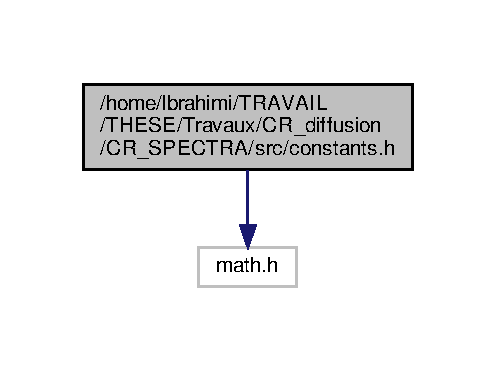
\includegraphics[width=238pt]{constants_8h__incl}
\end{center}
\end{figure}
This graph shows which files directly or indirectly include this file\+:\nopagebreak
\begin{figure}[H]
\begin{center}
\leavevmode
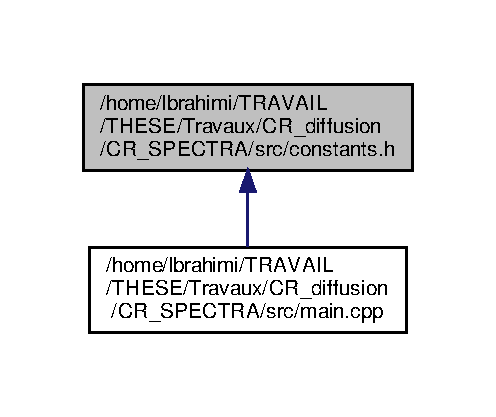
\includegraphics[width=238pt]{constants_8h__dep__incl}
\end{center}
\end{figure}
\subsection*{Variables}
\begin{DoxyCompactItemize}
\item 
const double \hyperlink{constants_8h_a43016d873124d39034edb8cd164794db}{pi} = 3.\+1472
\begin{DoxyCompactList}\small\item\em Inclusion of basic mathematic functions. \end{DoxyCompactList}\item 
const double \hyperlink{constants_8h_a1d183f5048588ce21c281b270591be80}{yr} = 3.\+154e+7
\item 
const double \hyperlink{constants_8h_a0edf155739e92555799f4a04b10af6bf}{kyr} = 1e3$\ast$yr
\begin{DoxyCompactList}\small\item\em 1 yr in \mbox{[}s\mbox{]} \end{DoxyCompactList}\item 
const double \hyperlink{constants_8h_aaf85ed8b741937db702f62aac693ae5d}{km} = 1e5
\begin{DoxyCompactList}\small\item\em 1 kyr in \mbox{[}s\mbox{]} \end{DoxyCompactList}\item 
const double \hyperlink{constants_8h_a2884cd030c4c825754349a525a1d06ce}{pc} = 3.\+086e18
\begin{DoxyCompactList}\small\item\em 1 km in \mbox{[}cm\mbox{]} \end{DoxyCompactList}\item 
const double \hyperlink{constants_8h_a1ec6fd9219412d45c0565c29304d5184}{kpc} = 1.e3$\ast$\hyperlink{constants_8h_a2884cd030c4c825754349a525a1d06ce}{pc}
\begin{DoxyCompactList}\small\item\em 1 pc in \mbox{[}cm\mbox{]} \end{DoxyCompactList}\item 
const double \hyperlink{constants_8h_aec0e126d9991db8ad0b26139f5860568}{GeV} = 0.\+00160218
\begin{DoxyCompactList}\small\item\em 1 kpc in \mbox{[}cm\mbox{]} \end{DoxyCompactList}\item 
const double \hyperlink{constants_8h_a7f801e1f6821bc6baf0652ed2496e5e9}{TeV} = 1e3$\ast$\+GeV
\begin{DoxyCompactList}\small\item\em 1 GeV in \mbox{[}erg\mbox{]} \end{DoxyCompactList}\item 
const double \hyperlink{constants_8h_a87b385f118e3715860117a77eda7136d}{eV} = \hyperlink{constants_8h_aec0e126d9991db8ad0b26139f5860568}{GeV}$\ast$1e-\/9
\begin{DoxyCompactList}\small\item\em 1 TeV in \mbox{[}erg\mbox{]} \end{DoxyCompactList}\item 
const double \hyperlink{constants_8h_ac90e720c4654493ae50b7b964cc6b20d}{MeV} = 1e-\/3$\ast$\+GeV
\begin{DoxyCompactList}\small\item\em 1 eV in \mbox{[}erg\mbox{]} \end{DoxyCompactList}\item 
const double \hyperlink{constants_8h_a6b331c08a80ed71d31c55a3341776483}{mp} = 1.\+6726219e-\/24
\begin{DoxyCompactList}\small\item\em 1 MeV in \mbox{[}erg\mbox{]} \end{DoxyCompactList}\item 
const double \hyperlink{constants_8h_affd3595ea3bf442893a3dc5bf568a663}{mn} = 1.\+6749286e-\/24
\begin{DoxyCompactList}\small\item\em Proton mass \mbox{[}g\mbox{]}. \end{DoxyCompactList}\item 
const double \hyperlink{constants_8h_a910e2c8f86d1b5103b0326aa65670e52}{me} = 9.\+1095e-\/28
\begin{DoxyCompactList}\small\item\em Neutron mass \mbox{[}g\mbox{]}. \end{DoxyCompactList}\item 
const double \hyperlink{constants_8h_a269606ec235d66ed4e8fc93442842cef}{m\+HI} = \hyperlink{constants_8h_a6b331c08a80ed71d31c55a3341776483}{mp}
\begin{DoxyCompactList}\small\item\em Electron mass \mbox{[}g\mbox{]}. \end{DoxyCompactList}\item 
const double \hyperlink{constants_8h_a469899272f9f1b48961397bbd6cc84eb}{m\+H\+II} = \hyperlink{constants_8h_a6b331c08a80ed71d31c55a3341776483}{mp}
\begin{DoxyCompactList}\small\item\em HI mass \mbox{[}g\mbox{]}. \end{DoxyCompactList}\item 
const double \hyperlink{constants_8h_a4158a5aec7d8c74f97fdbf32566a7fb6}{m\+HeI} = 2$\ast$\hyperlink{constants_8h_a6b331c08a80ed71d31c55a3341776483}{mp} + 2$\ast$\hyperlink{constants_8h_affd3595ea3bf442893a3dc5bf568a663}{mn}
\begin{DoxyCompactList}\small\item\em H\+II mass \mbox{[}g\mbox{]}. \end{DoxyCompactList}\item 
const double \hyperlink{constants_8h_ada6e925262426f66e688da4a131d25b2}{m\+C\+II} = 6$\ast$\hyperlink{constants_8h_a6b331c08a80ed71d31c55a3341776483}{mp} + 6$\ast$\hyperlink{constants_8h_affd3595ea3bf442893a3dc5bf568a663}{mn}
\begin{DoxyCompactList}\small\item\em HeI mass \mbox{[}g\mbox{]}. \end{DoxyCompactList}\item 
const double \hyperlink{constants_8h_a5636f746a8f39039b8377e515b50d69f}{m\+H2} = 2$\ast$\hyperlink{constants_8h_a6b331c08a80ed71d31c55a3341776483}{mp}
\begin{DoxyCompactList}\small\item\em C\+II mass \mbox{[}g\mbox{]}. \end{DoxyCompactList}\item 
const double \hyperlink{constants_8h_a2b076531cd50c7b55702a53221f2ac72}{e} = 4.\+80326e-\/10
\begin{DoxyCompactList}\small\item\em H2 mass \mbox{[}g\mbox{]}. \end{DoxyCompactList}\item 
const double \hyperlink{constants_8h_a8fc6defe4e499b1b9b9c275689e44352}{c} = 29979245800.
\begin{DoxyCompactList}\small\item\em e charge in \mbox{[}statC\mbox{]} \end{DoxyCompactList}\item 
const double \hyperlink{constants_8h_ae1187cd1ee5b820b4635b114ec498590}{kbolz} = 1.\+3807e-\/16
\begin{DoxyCompactList}\small\item\em light celerity in \mbox{[}cm/s\mbox{]} \end{DoxyCompactList}\item 
const double \hyperlink{constants_8h_a0eaab633bcaabbcea00dd832a7edaf65}{kms} = 1e5
\begin{DoxyCompactList}\small\item\em Boltzmann constant in C\+GS. \end{DoxyCompactList}\item 
const double \hyperlink{constants_8h_a88d6b9116f24d31fca76a2d49a5fcae4}{sig\+\_\+T} = 6.\+65e-\/25
\begin{DoxyCompactList}\small\item\em 1 km/s in cm/s \end{DoxyCompactList}\item 
const int \hyperlink{constants_8h_aa095316553501ccd88a1637ee4cab0cf}{solver\+\_\+\+Pcr\+Advection} = 1
\begin{DoxyCompactList}\small\item\em \mbox{[}cm$^\wedge$2\mbox{]} Thomson cross section (see Schlickeiser (2002) p.\+80) \end{DoxyCompactList}\item 
const int \hyperlink{constants_8h_ace4385eb1736e0034ec6652e790baaa1}{solver\+\_\+\+Pcr\+Diffusion} = 1
\begin{DoxyCompactList}\small\item\em Advective term of the CR Pressure (the classical one -\/$>$ V\+\_\+\+A$\ast$grad ...) \end{DoxyCompactList}\item 
const int \hyperlink{constants_8h_a852151594cb9244675e04b203ba3c87d}{solver\+\_\+\+Pcr\+Advection2} = 1
\begin{DoxyCompactList}\small\item\em Diffusive term of the CR Pressure. \end{DoxyCompactList}\item 
const int \hyperlink{constants_8h_afed28073f040247422af85d824631252}{solver\+\_\+\+Pcr\+AdvectionE} = 1
\begin{DoxyCompactList}\small\item\em Explicit Advection solver for Pcr by the energy derivative of Alfvén velocity. \end{DoxyCompactList}\item 
const int \hyperlink{constants_8h_a98d27ea3fbe9c4a26875f51eaa1df0a1}{solver\+\_\+\+Pcr\+Source1} = 1
\begin{DoxyCompactList}\small\item\em Explicit Advection solver for Pcr in energy cd\+V\+AdX. \end{DoxyCompactList}\item 
const int \hyperlink{constants_8h_a8f1a8ed5939dd4c75febe072ccd3f8d3}{solver\+\_\+\+Pcr\+Source2} = 1
\begin{DoxyCompactList}\small\item\em Source term effect due to the dependance of the Alfvén velocity to the space. \end{DoxyCompactList}\item 
const int \hyperlink{constants_8h_a82c88de5e5b11e9e548cea45ce018e70}{solver\+\_\+\+Pcr\+Perp\+Diff} = 0
\begin{DoxyCompactList}\small\item\em Source term effect due to the CR injection from the source in the system. \end{DoxyCompactList}\item 
const int \hyperlink{constants_8h_aa92635792000f78db2cda7adba7c29f1}{solver\+\_\+\+Pe\+Advection} = 1
\begin{DoxyCompactList}\small\item\em Perpendicular diffusion of C\+Rs after the coherence length. \end{DoxyCompactList}\item 
const int \hyperlink{constants_8h_ad4ac4c5a403c0893c414886ac425e6ed}{solver\+\_\+\+Pe\+Diffusion} = 1
\begin{DoxyCompactList}\small\item\em Advective term of the e-\/ Pressure (the classical one -\/$>$ V\+\_\+\+A$\ast$grad ...) \end{DoxyCompactList}\item 
const int \hyperlink{constants_8h_aaaabd43831d9596407b9e61f5ce39f8b}{solver\+\_\+\+Pe\+Advection2} = 1
\begin{DoxyCompactList}\small\item\em Diffusive term of the e-\/ Pressure. \end{DoxyCompactList}\item 
const int \hyperlink{constants_8h_a2b750aab67b75fb1b85fadd37813123d}{solver\+\_\+\+Pe\+AdvectionE} = 1
\begin{DoxyCompactList}\small\item\em Explicit Advection solver for e-\/ by the energy derivative of Alfvén velocity. \end{DoxyCompactList}\item 
const int \hyperlink{constants_8h_a5b37fca1d49e7b618e074df83ff912e9}{solver\+\_\+\+Pe\+Advection\+E1} = 1
\begin{DoxyCompactList}\small\item\em Explicit Advection solver for e-\/ in energy cd\+V\+AdX. \end{DoxyCompactList}\item 
const int \hyperlink{constants_8h_a49635eb66c973e50d41d2849dff11194}{solver\+\_\+\+Pe\+Advection\+E2} = 1
\begin{DoxyCompactList}\small\item\em Sychrotron radiations of e-\/ (looses of energy) -\/ Advection term. \end{DoxyCompactList}\item 
const int \hyperlink{constants_8h_a94c7e20be2baee4f40c05e12f47cb0cf}{solver\+\_\+\+Pe\+Source1} = 1
\begin{DoxyCompactList}\small\item\em Synchrotron radiations of e-\/ (looses of energy) -\/ source term. \end{DoxyCompactList}\item 
const int \hyperlink{constants_8h_ab9c3aa7f87b528ddb0ed9fb5c5b8d617}{solver\+\_\+\+Pe\+Source2} = 1
\begin{DoxyCompactList}\small\item\em Source term effect due to the dependance of the Alfvén velocity to the space (for e-\/) \end{DoxyCompactList}\item 
const int \hyperlink{constants_8h_adb61e67f736c5c0004396e27c21821fa}{solver\+\_\+\+Pe\+Perp\+Diff} = 0
\begin{DoxyCompactList}\small\item\em Source term effect due to the e-\/ injection from the source in the system. \end{DoxyCompactList}\item 
const int \hyperlink{constants_8h_ac65992d2fff2f4d8366fce54f9132144}{solver\+\_\+\+Ip\+Advection} = 1
\begin{DoxyCompactList}\small\item\em Perpendicular diffusion of e-\/ after the coherence length. \end{DoxyCompactList}\item 
const int \hyperlink{constants_8h_af67a2eb5a6e8985eeabd2f1ce6c2f60c}{solver\+\_\+\+Im\+Advection} = 1
\begin{DoxyCompactList}\small\item\em Advective term of the foward waves. \end{DoxyCompactList}\item 
const int \hyperlink{constants_8h_a50957b417603ffdeddb02966dc330e80}{solver\+\_\+\+Ip\+Source1} = 1
\begin{DoxyCompactList}\small\item\em Advective term of the backward waves. \end{DoxyCompactList}\item 
const int \hyperlink{constants_8h_a23b130a9818fa30a41bf8532f6ea05b6}{solver\+\_\+\+Im\+Source1} = 1
\begin{DoxyCompactList}\small\item\em Source term effect applied on foward waves due to the dependance of the Alfvén velocity to the space. \end{DoxyCompactList}\item 
const int \hyperlink{constants_8h_abfcf40c6374a94a91c1f34f1dd7a2d80}{solver\+\_\+\+Ip\+Damp\+Growth} = 1
\begin{DoxyCompactList}\small\item\em Source term effect applied on backward waves due to the dependance of the Alfvén velocity to the space. \end{DoxyCompactList}\item 
const int \hyperlink{constants_8h_a500d822bbc27b52a3dc510183dc11f61}{solver\+\_\+\+Im\+Damp\+Growth} = 1
\begin{DoxyCompactList}\small\item\em Source term effect due to production of self-\/turbulence -\/ damping applied on foward waves. \end{DoxyCompactList}\item 
const int \hyperlink{constants_8h_ac789867445186dfcef8b8ae68fb679c1}{solver\+\_\+\+Dilution} = 0
\begin{DoxyCompactList}\small\item\em Source term effect due to production of self-\/turbulence -\/ damping applied on backward waves. \end{DoxyCompactList}\item 
const int \hyperlink{constants_8h_a4c93f5a97d7c9ebea780b8f83d3230af}{set\+\_\+background} = 1
\item 
const double \hyperlink{constants_8h_ab8213b64ea2a6b866ce8d5eb0f0d3650}{step\+\_\+implicit} = 20.$\ast$\hyperlink{constants_8h_a1d183f5048588ce21c281b270591be80}{yr}
\begin{DoxyCompactList}\small\item\em If need to perform some test without background conditions (1 \+: On, 0 \+: off) \end{DoxyCompactList}\item 
const int \hyperlink{constants_8h_a597cb31f57e34e1df5d6306446baa554}{source\+\_\+terms\+\_\+exact} = 1
\item 
const int \hyperlink{constants_8h_a1b0d894b4d03ad0a2c1322d049fbbf8d}{nproc} = 1
\begin{DoxyCompactList}\small\item\em The way to solve the source terms \+: 1 -\/$>$ Exact solutions, 0 -\/$>$ 1st order numerical solution. \end{DoxyCompactList}\item 
const int \hyperlink{constants_8h_a2cb9c9fa2eae24bbb093a29295279de9}{output\+\_\+freq} = 0
\begin{DoxyCompactList}\small\item\em Number of processors for the run (! Still experimental) \end{DoxyCompactList}\item 
const double \hyperlink{constants_8h_abae1f83e3b8604181125a836accc1e95}{t\+\_\+data\+\_\+out\+\_\+min} = 0.$\ast$\hyperlink{constants_8h_a0edf155739e92555799f4a04b10af6bf}{kyr}
\begin{DoxyCompactList}\small\item\em Model of output frequency (0 \+: n output between t\+\_\+start and t\+\_\+end, 1 \+: 1 output each n timestep) n = number\+\_\+out\+\_\+data. \end{DoxyCompactList}\item 
const double \hyperlink{constants_8h_afac4a14af744124a25e6c88519faa007}{t\+\_\+data\+\_\+out\+\_\+max} = 500.$\ast$\hyperlink{constants_8h_a0edf155739e92555799f4a04b10af6bf}{kyr}
\begin{DoxyCompactList}\small\item\em Instant of the first output data. \end{DoxyCompactList}\item 
const int \hyperlink{constants_8h_a3765372d2b19c3cb81d33591f9d5b42b}{number\+\_\+out\+\_\+data} = 100
\begin{DoxyCompactList}\small\item\em 200.$\ast$kyr; Instant of the last output data \end{DoxyCompactList}\item 
const int \hyperlink{constants_8h_aad607c4a45df8deb54afd4536d608677}{time\+\_\+distrib\+\_\+of\+\_\+data} = 1
\begin{DoxyCompactList}\small\item\em Total number of output data. \end{DoxyCompactList}\item 
const double \hyperlink{constants_8h_a0fa0ccb487c38ac26d81804f004be860}{log\+\_\+first\+\_\+data} = 3e-\/1$\ast$kyr
\item 
const int \hyperlink{constants_8h_a9a692a1ef77cdf604ed460ed196a3241}{delta\+\_\+log\+\_\+output} = 100
\begin{DoxyCompactList}\small\item\em Time value of the first output in the logscaled output method. \end{DoxyCompactList}\item 
const double \hyperlink{constants_8h_a93e6f33b03669f059b9f0ec47810f624}{Tmax} = 500.\+1$\ast$\hyperlink{constants_8h_a0edf155739e92555799f4a04b10af6bf}{kyr}
\begin{DoxyCompactList}\small\item\em Number of time-\/step between two Log\+Output. \end{DoxyCompactList}\item 
const int \hyperlink{constants_8h_aa62928f1932e0d67ec2c1fe1546f5119}{verbose} = 0
\begin{DoxyCompactList}\small\item\em 200.\+1$\ast$kyr; Define the limit time of your simulation \end{DoxyCompactList}\item 
const double \hyperlink{constants_8h_a5739042d302439a74d32201d0e4d5437}{ttau\+\_\+sat} = -\/ log(0.\+1)/0.\+1
\begin{DoxyCompactList}\small\item\em 0 \+: False, 1 \+: True -\/$>$ Show extra informations during the simulation \end{DoxyCompactList}\item 
const double \hyperlink{constants_8h_a9b9d18e30a29306436fa5734a8c82f00}{Esn} = 1
\item 
const double \hyperlink{constants_8h_a8d1741e252e623a3e1ef195fa5a96ede}{Mej} = 1
\begin{DoxyCompactList}\small\item\em in units of 1e51 erg \+: total energy released by S\+NR \end{DoxyCompactList}\item 
const double \hyperlink{constants_8h_afa9a0679a224d46d61198ff6c614ffe8}{xi\+\_\+n} = 1
\begin{DoxyCompactList}\small\item\em Msun \+: total mass released by S\+NR in sun mass units. \end{DoxyCompactList}\item 
const double \hyperlink{constants_8h_a1bdb9cc12446f64f0ba598530df12971}{phi\+\_\+c} = 1
\begin{DoxyCompactList}\small\item\em For solar abundances. \end{DoxyCompactList}\item 
const double \hyperlink{constants_8h_a2f8a70c47ded89b686c28afb42e37a02}{bbeta} = 2
\begin{DoxyCompactList}\small\item\em Actual thermal cond. / the Sptitzer (1962) value. \end{DoxyCompactList}\item 
const double \hyperlink{constants_8h_a909ecc3296d02720b96a3d5bd61169f8}{C06} = 1.
\item 
const double \hyperlink{constants_8h_a15ee6bd88a32248212e10c43f5723f79}{xhi\+\_\+cr} = 0.\+1
\item 
const double \hyperlink{constants_8h_ab3fe7c05540f838431e564ab6fca7205}{xhi\+\_\+0} = 2.\+026
\begin{DoxyCompactList}\small\item\em Efficiency of C\+Rs acceleration. \end{DoxyCompactList}\item 
const double \hyperlink{constants_8h_a30fd985a45c0aac1337c39ec204848e4}{gam} = 2.\+2
\item 
const int \hyperlink{constants_8h_a5119c36ba4a00630b7181d16049cc5e8}{injection\+\_\+cutoff} = 0
\begin{DoxyCompactList}\small\item\em C\+Rs injection energy power law index. \end{DoxyCompactList}\item 
const double \hyperlink{constants_8h_ae38d64b4a117699b463b9231bb67bf54}{inj\+\_\+exp\+\_\+alpha} = 1
\item 
const double \hyperlink{constants_8h_a068ac4242a1fc9e4ba016240976d16ae}{Emin} = 0.\+1$\ast$\hyperlink{constants_8h_aec0e126d9991db8ad0b26139f5860568}{GeV}
\begin{DoxyCompactList}\small\item\em Factor of the exponential cutoff in the C\+Rs injection spectra (d\+N(\+E)/dE $\sim$ exp(-\/inj\+\_\+exp\+\_\+alpha$\ast$\+E/\+E\+\_\+\+Max)) \end{DoxyCompactList}\item 
const double \hyperlink{constants_8h_a80a3c65c6b77216165fc34c12d0744e9}{delta} = 4.
\begin{DoxyCompactList}\small\item\em Minimum accelered C\+Rs during the Sedov phase. \end{DoxyCompactList}\item 
const int \hyperlink{constants_8h_a6c6aaf5c178c86cf4dab308f1e6d3704}{injection\+\_\+shape\+\_\+time} = 0
\begin{DoxyCompactList}\small\item\em From Celli et al. (2019) -\/ see Brahimi et al. (2020) \end{DoxyCompactList}\item 
const double \hyperlink{constants_8h_a9b20d821a97295f5510e0143c8dbcf53}{t\+\_\+start\+\_\+injection} = 1e-\/6$\ast$kyr
\begin{DoxyCompactList}\small\item\em 0 \+: Time Dirac C\+Rs, 1 \+: Time Gaussian C\+Rs \end{DoxyCompactList}\item 
const double \hyperlink{constants_8h_a041792abd5b56a3c756afdffaf574f83}{t\+\_\+end\+\_\+injection} = 2
\begin{DoxyCompactList}\small\item\em Time start C\+Rs injection function. \end{DoxyCompactList}\item 
const double \hyperlink{constants_8h_a2a83e185b1c5f11c0b2d666fb3349262}{injection\+\_\+function\+\_\+width} = 10.
\begin{DoxyCompactList}\small\item\em \mbox{[}in tesc\mbox{[}E\mbox{]} units\mbox{]} Time end C\+Rs injection function (number of tesc) \end{DoxyCompactList}\item 
const int \hyperlink{constants_8h_af382d07a9e39728e9cc31cee2c20e45a}{injection\+\_\+function\+\_\+norm} = 1000
\item 
const double \hyperlink{constants_8h_a6f13fdab62a279c2dc33ec6c216726c9}{r\+\_\+snr\+\_\+thickness} = 100
\begin{DoxyCompactList}\small\item\em Constant in order to easily and rapidly normalize the injection function. \end{DoxyCompactList}\item 
const double \hyperlink{constants_8h_a899c4902b6fa71ee29d2cec69f63788d}{electron\+\_\+injection\+\_\+rate} = 1e-\/2
\begin{DoxyCompactList}\small\item\em = R\+\_\+\+S\+N\+R(t)/by the value you chose, it allows to smooth the injection shape of C\+Rs \end{DoxyCompactList}\item 
const int \hyperlink{constants_8h_a86a818aa1e9ae9a5fcca86cfcca630ba}{tesc\+\_\+model} = 1
\begin{DoxyCompactList}\small\item\em Corresponds to the energy injected in the electron spectrum compared to the energy injected in the proton spectrum. \end{DoxyCompactList}\item 
const int \hyperlink{constants_8h_acf3c464056cb177d978eb559b005d19e}{oh\+\_\+model} = 3
\item 
const double \hyperlink{constants_8h_aeecaff5947ca8d511bb3b7751e9199ef}{eta\+\_\+gfree} = 1
\item 
const double \hyperlink{constants_8h_a7dd0fdc6bda4f1811187b7e6f8e73812}{eta\+\_\+acc} = 10
\item 
const double \hyperlink{constants_8h_a2b0717ef84f43e2da8a080becfb72cc7}{Eknee} = 1e15$\ast$eV
\item 
const double \hyperlink{constants_8h_adeedc97114c5a704906c8e26bdbd2451}{alpha} = 2.\+6
\item 
const double \hyperlink{constants_8h_a94e9e399494c25eeaa56ef7c088b1e38}{coherence\+\_\+length} = 100$\ast$\hyperlink{constants_8h_a2884cd030c4c825754349a525a1d06ce}{pc}
\item 
const double \hyperlink{constants_8h_a2cd2bb5c17eb3c354f7e9c8aec991e02}{sigma\+\_\+coherence} = 10$\ast$\hyperlink{constants_8h_a2884cd030c4c825754349a525a1d06ce}{pc}
\begin{DoxyCompactList}\small\item\em Coherence length of the magnetic field. \end{DoxyCompactList}\item 
const double \hyperlink{constants_8h_ac435337b81e4a235f21e6374c911d294}{isotropy} = 1
\end{DoxyCompactItemize}


\subsection{Variable Documentation}
\mbox{\Hypertarget{constants_8h_adeedc97114c5a704906c8e26bdbd2451}\label{constants_8h_adeedc97114c5a704906c8e26bdbd2451}} 
\index{constants.\+h@{constants.\+h}!alpha@{alpha}}
\index{alpha@{alpha}!constants.\+h@{constants.\+h}}
\subsubsection{\texorpdfstring{alpha}{alpha}}
{\footnotesize\ttfamily const double alpha = 2.\+6}

\mbox{\Hypertarget{constants_8h_a2f8a70c47ded89b686c28afb42e37a02}\label{constants_8h_a2f8a70c47ded89b686c28afb42e37a02}} 
\index{constants.\+h@{constants.\+h}!bbeta@{bbeta}}
\index{bbeta@{bbeta}!constants.\+h@{constants.\+h}}
\subsubsection{\texorpdfstring{bbeta}{bbeta}}
{\footnotesize\ttfamily const double bbeta = 2}



Actual thermal cond. / the Sptitzer (1962) value. 

\mbox{\Hypertarget{constants_8h_a8fc6defe4e499b1b9b9c275689e44352}\label{constants_8h_a8fc6defe4e499b1b9b9c275689e44352}} 
\index{constants.\+h@{constants.\+h}!c@{c}}
\index{c@{c}!constants.\+h@{constants.\+h}}
\subsubsection{\texorpdfstring{c}{c}}
{\footnotesize\ttfamily const double c = 29979245800.}



e charge in \mbox{[}statC\mbox{]} 

\mbox{\Hypertarget{constants_8h_a909ecc3296d02720b96a3d5bd61169f8}\label{constants_8h_a909ecc3296d02720b96a3d5bd61169f8}} 
\index{constants.\+h@{constants.\+h}!C06@{C06}}
\index{C06@{C06}!constants.\+h@{constants.\+h}}
\subsubsection{\texorpdfstring{C06}{C06}}
{\footnotesize\ttfamily const double C06 = 1.}

\mbox{\Hypertarget{constants_8h_a94e9e399494c25eeaa56ef7c088b1e38}\label{constants_8h_a94e9e399494c25eeaa56ef7c088b1e38}} 
\index{constants.\+h@{constants.\+h}!coherence\+\_\+length@{coherence\+\_\+length}}
\index{coherence\+\_\+length@{coherence\+\_\+length}!constants.\+h@{constants.\+h}}
\subsubsection{\texorpdfstring{coherence\+\_\+length}{coherence\_length}}
{\footnotesize\ttfamily const double coherence\+\_\+length = 100$\ast$\hyperlink{constants_8h_a2884cd030c4c825754349a525a1d06ce}{pc}}

\mbox{\Hypertarget{constants_8h_a80a3c65c6b77216165fc34c12d0744e9}\label{constants_8h_a80a3c65c6b77216165fc34c12d0744e9}} 
\index{constants.\+h@{constants.\+h}!delta@{delta}}
\index{delta@{delta}!constants.\+h@{constants.\+h}}
\subsubsection{\texorpdfstring{delta}{delta}}
{\footnotesize\ttfamily const double delta = 4.}



Minimum accelered C\+Rs during the Sedov phase. 

\mbox{\Hypertarget{constants_8h_a9a692a1ef77cdf604ed460ed196a3241}\label{constants_8h_a9a692a1ef77cdf604ed460ed196a3241}} 
\index{constants.\+h@{constants.\+h}!delta\+\_\+log\+\_\+output@{delta\+\_\+log\+\_\+output}}
\index{delta\+\_\+log\+\_\+output@{delta\+\_\+log\+\_\+output}!constants.\+h@{constants.\+h}}
\subsubsection{\texorpdfstring{delta\+\_\+log\+\_\+output}{delta\_log\_output}}
{\footnotesize\ttfamily const int delta\+\_\+log\+\_\+output = 100}



Time value of the first output in the logscaled output method. 

\mbox{\Hypertarget{constants_8h_a2b076531cd50c7b55702a53221f2ac72}\label{constants_8h_a2b076531cd50c7b55702a53221f2ac72}} 
\index{constants.\+h@{constants.\+h}!e@{e}}
\index{e@{e}!constants.\+h@{constants.\+h}}
\subsubsection{\texorpdfstring{e}{e}}
{\footnotesize\ttfamily const double e = 4.\+80326e-\/10}



H2 mass \mbox{[}g\mbox{]}. 

\mbox{\Hypertarget{constants_8h_a2b0717ef84f43e2da8a080becfb72cc7}\label{constants_8h_a2b0717ef84f43e2da8a080becfb72cc7}} 
\index{constants.\+h@{constants.\+h}!Eknee@{Eknee}}
\index{Eknee@{Eknee}!constants.\+h@{constants.\+h}}
\subsubsection{\texorpdfstring{Eknee}{Eknee}}
{\footnotesize\ttfamily const double Eknee = 1e15$\ast$eV}

\mbox{\Hypertarget{constants_8h_a899c4902b6fa71ee29d2cec69f63788d}\label{constants_8h_a899c4902b6fa71ee29d2cec69f63788d}} 
\index{constants.\+h@{constants.\+h}!electron\+\_\+injection\+\_\+rate@{electron\+\_\+injection\+\_\+rate}}
\index{electron\+\_\+injection\+\_\+rate@{electron\+\_\+injection\+\_\+rate}!constants.\+h@{constants.\+h}}
\subsubsection{\texorpdfstring{electron\+\_\+injection\+\_\+rate}{electron\_injection\_rate}}
{\footnotesize\ttfamily const double electron\+\_\+injection\+\_\+rate = 1e-\/2}



= R\+\_\+\+S\+N\+R(t)/by the value you chose, it allows to smooth the injection shape of C\+Rs 

\mbox{\Hypertarget{constants_8h_a068ac4242a1fc9e4ba016240976d16ae}\label{constants_8h_a068ac4242a1fc9e4ba016240976d16ae}} 
\index{constants.\+h@{constants.\+h}!Emin@{Emin}}
\index{Emin@{Emin}!constants.\+h@{constants.\+h}}
\subsubsection{\texorpdfstring{Emin}{Emin}}
{\footnotesize\ttfamily const double Emin = 0.\+1$\ast$\hyperlink{constants_8h_aec0e126d9991db8ad0b26139f5860568}{GeV}}



Factor of the exponential cutoff in the C\+Rs injection spectra (d\+N(\+E)/dE $\sim$ exp(-\/inj\+\_\+exp\+\_\+alpha$\ast$\+E/\+E\+\_\+\+Max)) 

\mbox{\Hypertarget{constants_8h_a9b9d18e30a29306436fa5734a8c82f00}\label{constants_8h_a9b9d18e30a29306436fa5734a8c82f00}} 
\index{constants.\+h@{constants.\+h}!Esn@{Esn}}
\index{Esn@{Esn}!constants.\+h@{constants.\+h}}
\subsubsection{\texorpdfstring{Esn}{Esn}}
{\footnotesize\ttfamily const double Esn = 1}

Growth waves saturation rate
\begin{DoxyItemize}
\item log(0.\+1)/0.1; Has the form -\/ log(a)/b where b \+: characteristic max value, a \+: suppression factor after b, ttau\+\_\+sat = 0 -\/$>$ Linear growth This term is still experimental 
\end{DoxyItemize}\mbox{\Hypertarget{constants_8h_a7dd0fdc6bda4f1811187b7e6f8e73812}\label{constants_8h_a7dd0fdc6bda4f1811187b7e6f8e73812}} 
\index{constants.\+h@{constants.\+h}!eta\+\_\+acc@{eta\+\_\+acc}}
\index{eta\+\_\+acc@{eta\+\_\+acc}!constants.\+h@{constants.\+h}}
\subsubsection{\texorpdfstring{eta\+\_\+acc}{eta\_acc}}
{\footnotesize\ttfamily const double eta\+\_\+acc = 10}

\mbox{\Hypertarget{constants_8h_aeecaff5947ca8d511bb3b7751e9199ef}\label{constants_8h_aeecaff5947ca8d511bb3b7751e9199ef}} 
\index{constants.\+h@{constants.\+h}!eta\+\_\+gfree@{eta\+\_\+gfree}}
\index{eta\+\_\+gfree@{eta\+\_\+gfree}!constants.\+h@{constants.\+h}}
\subsubsection{\texorpdfstring{eta\+\_\+gfree}{eta\_gfree}}
{\footnotesize\ttfamily const double eta\+\_\+gfree = 1}

\mbox{\Hypertarget{constants_8h_a87b385f118e3715860117a77eda7136d}\label{constants_8h_a87b385f118e3715860117a77eda7136d}} 
\index{constants.\+h@{constants.\+h}!eV@{eV}}
\index{eV@{eV}!constants.\+h@{constants.\+h}}
\subsubsection{\texorpdfstring{eV}{eV}}
{\footnotesize\ttfamily const double eV = \hyperlink{constants_8h_aec0e126d9991db8ad0b26139f5860568}{GeV}$\ast$1e-\/9}



1 TeV in \mbox{[}erg\mbox{]} 

\mbox{\Hypertarget{constants_8h_a30fd985a45c0aac1337c39ec204848e4}\label{constants_8h_a30fd985a45c0aac1337c39ec204848e4}} 
\index{constants.\+h@{constants.\+h}!gam@{gam}}
\index{gam@{gam}!constants.\+h@{constants.\+h}}
\subsubsection{\texorpdfstring{gam}{gam}}
{\footnotesize\ttfamily const double gam = 2.\+2}

\mbox{\Hypertarget{constants_8h_aec0e126d9991db8ad0b26139f5860568}\label{constants_8h_aec0e126d9991db8ad0b26139f5860568}} 
\index{constants.\+h@{constants.\+h}!GeV@{GeV}}
\index{GeV@{GeV}!constants.\+h@{constants.\+h}}
\subsubsection{\texorpdfstring{GeV}{GeV}}
{\footnotesize\ttfamily const double GeV = 0.\+00160218}



1 kpc in \mbox{[}cm\mbox{]} 

\mbox{\Hypertarget{constants_8h_ae38d64b4a117699b463b9231bb67bf54}\label{constants_8h_ae38d64b4a117699b463b9231bb67bf54}} 
\index{constants.\+h@{constants.\+h}!inj\+\_\+exp\+\_\+alpha@{inj\+\_\+exp\+\_\+alpha}}
\index{inj\+\_\+exp\+\_\+alpha@{inj\+\_\+exp\+\_\+alpha}!constants.\+h@{constants.\+h}}
\subsubsection{\texorpdfstring{inj\+\_\+exp\+\_\+alpha}{inj\_exp\_alpha}}
{\footnotesize\ttfamily const double inj\+\_\+exp\+\_\+alpha = 1}

Cut-\/off kind of the C\+Rs injection spectra ( 0 \+: Abrupt no smooth, 1 \+: Exponential\+\_\+cutoff see. inj\+\_\+exp\+\_\+alpha) Note \+: This model is only applicable to the proton spectrum. For electrons, the injection spectrum will be automatically cut by the synchrotron radiations \mbox{\Hypertarget{constants_8h_a5119c36ba4a00630b7181d16049cc5e8}\label{constants_8h_a5119c36ba4a00630b7181d16049cc5e8}} 
\index{constants.\+h@{constants.\+h}!injection\+\_\+cutoff@{injection\+\_\+cutoff}}
\index{injection\+\_\+cutoff@{injection\+\_\+cutoff}!constants.\+h@{constants.\+h}}
\subsubsection{\texorpdfstring{injection\+\_\+cutoff}{injection\_cutoff}}
{\footnotesize\ttfamily const int injection\+\_\+cutoff = 0}



C\+Rs injection energy power law index. 

\mbox{\Hypertarget{constants_8h_af382d07a9e39728e9cc31cee2c20e45a}\label{constants_8h_af382d07a9e39728e9cc31cee2c20e45a}} 
\index{constants.\+h@{constants.\+h}!injection\+\_\+function\+\_\+norm@{injection\+\_\+function\+\_\+norm}}
\index{injection\+\_\+function\+\_\+norm@{injection\+\_\+function\+\_\+norm}!constants.\+h@{constants.\+h}}
\subsubsection{\texorpdfstring{injection\+\_\+function\+\_\+norm}{injection\_function\_norm}}
{\footnotesize\ttfamily const int injection\+\_\+function\+\_\+norm = 1000}

Corresponds approximately to the width of the escape time divided (take care \+: too high value may affect the calculation and create noise) Max value -\/$>$ value such as the width of Finj $>$$>$ dt, max recommended value = 10 for NX,NE = 10, 7 \mbox{\Hypertarget{constants_8h_a2a83e185b1c5f11c0b2d666fb3349262}\label{constants_8h_a2a83e185b1c5f11c0b2d666fb3349262}} 
\index{constants.\+h@{constants.\+h}!injection\+\_\+function\+\_\+width@{injection\+\_\+function\+\_\+width}}
\index{injection\+\_\+function\+\_\+width@{injection\+\_\+function\+\_\+width}!constants.\+h@{constants.\+h}}
\subsubsection{\texorpdfstring{injection\+\_\+function\+\_\+width}{injection\_function\_width}}
{\footnotesize\ttfamily const double injection\+\_\+function\+\_\+width = 10.}



\mbox{[}in tesc\mbox{[}E\mbox{]} units\mbox{]} Time end C\+Rs injection function (number of tesc) 

\mbox{\Hypertarget{constants_8h_a6c6aaf5c178c86cf4dab308f1e6d3704}\label{constants_8h_a6c6aaf5c178c86cf4dab308f1e6d3704}} 
\index{constants.\+h@{constants.\+h}!injection\+\_\+shape\+\_\+time@{injection\+\_\+shape\+\_\+time}}
\index{injection\+\_\+shape\+\_\+time@{injection\+\_\+shape\+\_\+time}!constants.\+h@{constants.\+h}}
\subsubsection{\texorpdfstring{injection\+\_\+shape\+\_\+time}{injection\_shape\_time}}
{\footnotesize\ttfamily const int injection\+\_\+shape\+\_\+time = 0}



From Celli et al. (2019) -\/ see Brahimi et al. (2020) 

\mbox{\Hypertarget{constants_8h_ac435337b81e4a235f21e6374c911d294}\label{constants_8h_ac435337b81e4a235f21e6374c911d294}} 
\index{constants.\+h@{constants.\+h}!isotropy@{isotropy}}
\index{isotropy@{isotropy}!constants.\+h@{constants.\+h}}
\subsubsection{\texorpdfstring{isotropy}{isotropy}}
{\footnotesize\ttfamily const double isotropy = 1}

Width of the transition from the part close to the source where the diffusion coefficient is anitropic and the part far from the source where the diffusion is isotropic \mbox{\Hypertarget{constants_8h_ae1187cd1ee5b820b4635b114ec498590}\label{constants_8h_ae1187cd1ee5b820b4635b114ec498590}} 
\index{constants.\+h@{constants.\+h}!kbolz@{kbolz}}
\index{kbolz@{kbolz}!constants.\+h@{constants.\+h}}
\subsubsection{\texorpdfstring{kbolz}{kbolz}}
{\footnotesize\ttfamily const double kbolz = 1.\+3807e-\/16}



light celerity in \mbox{[}cm/s\mbox{]} 

\mbox{\Hypertarget{constants_8h_aaf85ed8b741937db702f62aac693ae5d}\label{constants_8h_aaf85ed8b741937db702f62aac693ae5d}} 
\index{constants.\+h@{constants.\+h}!km@{km}}
\index{km@{km}!constants.\+h@{constants.\+h}}
\subsubsection{\texorpdfstring{km}{km}}
{\footnotesize\ttfamily const double km = 1e5}



1 kyr in \mbox{[}s\mbox{]} 

\mbox{\Hypertarget{constants_8h_a0eaab633bcaabbcea00dd832a7edaf65}\label{constants_8h_a0eaab633bcaabbcea00dd832a7edaf65}} 
\index{constants.\+h@{constants.\+h}!kms@{kms}}
\index{kms@{kms}!constants.\+h@{constants.\+h}}
\subsubsection{\texorpdfstring{kms}{kms}}
{\footnotesize\ttfamily const double kms = 1e5}



Boltzmann constant in C\+GS. 

\mbox{\Hypertarget{constants_8h_a1ec6fd9219412d45c0565c29304d5184}\label{constants_8h_a1ec6fd9219412d45c0565c29304d5184}} 
\index{constants.\+h@{constants.\+h}!kpc@{kpc}}
\index{kpc@{kpc}!constants.\+h@{constants.\+h}}
\subsubsection{\texorpdfstring{kpc}{kpc}}
{\footnotesize\ttfamily const double kpc = 1.e3$\ast$\hyperlink{constants_8h_a2884cd030c4c825754349a525a1d06ce}{pc}}



1 pc in \mbox{[}cm\mbox{]} 

\mbox{\Hypertarget{constants_8h_a0edf155739e92555799f4a04b10af6bf}\label{constants_8h_a0edf155739e92555799f4a04b10af6bf}} 
\index{constants.\+h@{constants.\+h}!kyr@{kyr}}
\index{kyr@{kyr}!constants.\+h@{constants.\+h}}
\subsubsection{\texorpdfstring{kyr}{kyr}}
{\footnotesize\ttfamily const double kyr = 1e3$\ast$yr}



1 yr in \mbox{[}s\mbox{]} 

\mbox{\Hypertarget{constants_8h_a0fa0ccb487c38ac26d81804f004be860}\label{constants_8h_a0fa0ccb487c38ac26d81804f004be860}} 
\index{constants.\+h@{constants.\+h}!log\+\_\+first\+\_\+data@{log\+\_\+first\+\_\+data}}
\index{log\+\_\+first\+\_\+data@{log\+\_\+first\+\_\+data}!constants.\+h@{constants.\+h}}
\subsubsection{\texorpdfstring{log\+\_\+first\+\_\+data}{log\_first\_data}}
{\footnotesize\ttfamily const double log\+\_\+first\+\_\+data = 3e-\/1$\ast$kyr}

Time distribution of output data (0 \+: linspace, 1 \+: log10-\/space 2 \+: Custom output times, see the function \hyperlink{out_8h_a1b96bfc105db29caefe0dedd06daf16d}{specific\+Output\+Data()} in the file \+: \hyperlink{out_8h}{out.\+h}) \mbox{\Hypertarget{constants_8h_ada6e925262426f66e688da4a131d25b2}\label{constants_8h_ada6e925262426f66e688da4a131d25b2}} 
\index{constants.\+h@{constants.\+h}!m\+C\+II@{m\+C\+II}}
\index{m\+C\+II@{m\+C\+II}!constants.\+h@{constants.\+h}}
\subsubsection{\texorpdfstring{m\+C\+II}{mCII}}
{\footnotesize\ttfamily const double m\+C\+II = 6$\ast$\hyperlink{constants_8h_a6b331c08a80ed71d31c55a3341776483}{mp} + 6$\ast$\hyperlink{constants_8h_affd3595ea3bf442893a3dc5bf568a663}{mn}}



HeI mass \mbox{[}g\mbox{]}. 

\mbox{\Hypertarget{constants_8h_a910e2c8f86d1b5103b0326aa65670e52}\label{constants_8h_a910e2c8f86d1b5103b0326aa65670e52}} 
\index{constants.\+h@{constants.\+h}!me@{me}}
\index{me@{me}!constants.\+h@{constants.\+h}}
\subsubsection{\texorpdfstring{me}{me}}
{\footnotesize\ttfamily const double me = 9.\+1095e-\/28}



Neutron mass \mbox{[}g\mbox{]}. 

\mbox{\Hypertarget{constants_8h_a8d1741e252e623a3e1ef195fa5a96ede}\label{constants_8h_a8d1741e252e623a3e1ef195fa5a96ede}} 
\index{constants.\+h@{constants.\+h}!Mej@{Mej}}
\index{Mej@{Mej}!constants.\+h@{constants.\+h}}
\subsubsection{\texorpdfstring{Mej}{Mej}}
{\footnotesize\ttfamily const double Mej = 1}



in units of 1e51 erg \+: total energy released by S\+NR 

\mbox{\Hypertarget{constants_8h_ac90e720c4654493ae50b7b964cc6b20d}\label{constants_8h_ac90e720c4654493ae50b7b964cc6b20d}} 
\index{constants.\+h@{constants.\+h}!MeV@{MeV}}
\index{MeV@{MeV}!constants.\+h@{constants.\+h}}
\subsubsection{\texorpdfstring{MeV}{MeV}}
{\footnotesize\ttfamily const double MeV = 1e-\/3$\ast$\+GeV}



1 eV in \mbox{[}erg\mbox{]} 

\mbox{\Hypertarget{constants_8h_a5636f746a8f39039b8377e515b50d69f}\label{constants_8h_a5636f746a8f39039b8377e515b50d69f}} 
\index{constants.\+h@{constants.\+h}!m\+H2@{m\+H2}}
\index{m\+H2@{m\+H2}!constants.\+h@{constants.\+h}}
\subsubsection{\texorpdfstring{m\+H2}{mH2}}
{\footnotesize\ttfamily const double m\+H2 = 2$\ast$\hyperlink{constants_8h_a6b331c08a80ed71d31c55a3341776483}{mp}}



C\+II mass \mbox{[}g\mbox{]}. 

\mbox{\Hypertarget{constants_8h_a4158a5aec7d8c74f97fdbf32566a7fb6}\label{constants_8h_a4158a5aec7d8c74f97fdbf32566a7fb6}} 
\index{constants.\+h@{constants.\+h}!m\+HeI@{m\+HeI}}
\index{m\+HeI@{m\+HeI}!constants.\+h@{constants.\+h}}
\subsubsection{\texorpdfstring{m\+HeI}{mHeI}}
{\footnotesize\ttfamily const double m\+HeI = 2$\ast$\hyperlink{constants_8h_a6b331c08a80ed71d31c55a3341776483}{mp} + 2$\ast$\hyperlink{constants_8h_affd3595ea3bf442893a3dc5bf568a663}{mn}}



H\+II mass \mbox{[}g\mbox{]}. 

\mbox{\Hypertarget{constants_8h_a269606ec235d66ed4e8fc93442842cef}\label{constants_8h_a269606ec235d66ed4e8fc93442842cef}} 
\index{constants.\+h@{constants.\+h}!m\+HI@{m\+HI}}
\index{m\+HI@{m\+HI}!constants.\+h@{constants.\+h}}
\subsubsection{\texorpdfstring{m\+HI}{mHI}}
{\footnotesize\ttfamily const double m\+HI = \hyperlink{constants_8h_a6b331c08a80ed71d31c55a3341776483}{mp}}



Electron mass \mbox{[}g\mbox{]}. 

\mbox{\Hypertarget{constants_8h_a469899272f9f1b48961397bbd6cc84eb}\label{constants_8h_a469899272f9f1b48961397bbd6cc84eb}} 
\index{constants.\+h@{constants.\+h}!m\+H\+II@{m\+H\+II}}
\index{m\+H\+II@{m\+H\+II}!constants.\+h@{constants.\+h}}
\subsubsection{\texorpdfstring{m\+H\+II}{mHII}}
{\footnotesize\ttfamily const double m\+H\+II = \hyperlink{constants_8h_a6b331c08a80ed71d31c55a3341776483}{mp}}



HI mass \mbox{[}g\mbox{]}. 

\mbox{\Hypertarget{constants_8h_affd3595ea3bf442893a3dc5bf568a663}\label{constants_8h_affd3595ea3bf442893a3dc5bf568a663}} 
\index{constants.\+h@{constants.\+h}!mn@{mn}}
\index{mn@{mn}!constants.\+h@{constants.\+h}}
\subsubsection{\texorpdfstring{mn}{mn}}
{\footnotesize\ttfamily const double mn = 1.\+6749286e-\/24}



Proton mass \mbox{[}g\mbox{]}. 

\mbox{\Hypertarget{constants_8h_a6b331c08a80ed71d31c55a3341776483}\label{constants_8h_a6b331c08a80ed71d31c55a3341776483}} 
\index{constants.\+h@{constants.\+h}!mp@{mp}}
\index{mp@{mp}!constants.\+h@{constants.\+h}}
\subsubsection{\texorpdfstring{mp}{mp}}
{\footnotesize\ttfamily const double mp = 1.\+6726219e-\/24}



1 MeV in \mbox{[}erg\mbox{]} 

\mbox{\Hypertarget{constants_8h_a1b0d894b4d03ad0a2c1322d049fbbf8d}\label{constants_8h_a1b0d894b4d03ad0a2c1322d049fbbf8d}} 
\index{constants.\+h@{constants.\+h}!nproc@{nproc}}
\index{nproc@{nproc}!constants.\+h@{constants.\+h}}
\subsubsection{\texorpdfstring{nproc}{nproc}}
{\footnotesize\ttfamily const int nproc = 1}



The way to solve the source terms \+: 1 -\/$>$ Exact solutions, 0 -\/$>$ 1st order numerical solution. 

\mbox{\Hypertarget{constants_8h_a3765372d2b19c3cb81d33591f9d5b42b}\label{constants_8h_a3765372d2b19c3cb81d33591f9d5b42b}} 
\index{constants.\+h@{constants.\+h}!number\+\_\+out\+\_\+data@{number\+\_\+out\+\_\+data}}
\index{number\+\_\+out\+\_\+data@{number\+\_\+out\+\_\+data}!constants.\+h@{constants.\+h}}
\subsubsection{\texorpdfstring{number\+\_\+out\+\_\+data}{number\_out\_data}}
{\footnotesize\ttfamily const int number\+\_\+out\+\_\+data = 100}



200.$\ast$kyr; Instant of the last output data 

\mbox{\Hypertarget{constants_8h_acf3c464056cb177d978eb559b005d19e}\label{constants_8h_acf3c464056cb177d978eb559b005d19e}} 
\index{constants.\+h@{constants.\+h}!oh\+\_\+model@{oh\+\_\+model}}
\index{oh\+\_\+model@{oh\+\_\+model}!constants.\+h@{constants.\+h}}
\subsubsection{\texorpdfstring{oh\+\_\+model}{oh\_model}}
{\footnotesize\ttfamily const int oh\+\_\+model = 3}

CR escape time model (1 \+: All C\+Rs escape at the begining of the radiative phase, 2 \+: If v\+\_\+sh $<$ 110 km/s, all C\+Rs escape, 0 \+: No radiative escape model) \mbox{\Hypertarget{constants_8h_a2cb9c9fa2eae24bbb093a29295279de9}\label{constants_8h_a2cb9c9fa2eae24bbb093a29295279de9}} 
\index{constants.\+h@{constants.\+h}!output\+\_\+freq@{output\+\_\+freq}}
\index{output\+\_\+freq@{output\+\_\+freq}!constants.\+h@{constants.\+h}}
\subsubsection{\texorpdfstring{output\+\_\+freq}{output\_freq}}
{\footnotesize\ttfamily const int output\+\_\+freq = 0}



Number of processors for the run (! Still experimental) 

\mbox{\Hypertarget{constants_8h_a2884cd030c4c825754349a525a1d06ce}\label{constants_8h_a2884cd030c4c825754349a525a1d06ce}} 
\index{constants.\+h@{constants.\+h}!pc@{pc}}
\index{pc@{pc}!constants.\+h@{constants.\+h}}
\subsubsection{\texorpdfstring{pc}{pc}}
{\footnotesize\ttfamily const double pc = 3.\+086e18}



1 km in \mbox{[}cm\mbox{]} 

\mbox{\Hypertarget{constants_8h_a1bdb9cc12446f64f0ba598530df12971}\label{constants_8h_a1bdb9cc12446f64f0ba598530df12971}} 
\index{constants.\+h@{constants.\+h}!phi\+\_\+c@{phi\+\_\+c}}
\index{phi\+\_\+c@{phi\+\_\+c}!constants.\+h@{constants.\+h}}
\subsubsection{\texorpdfstring{phi\+\_\+c}{phi\_c}}
{\footnotesize\ttfamily const double phi\+\_\+c = 1}



For solar abundances. 

\mbox{\Hypertarget{constants_8h_a43016d873124d39034edb8cd164794db}\label{constants_8h_a43016d873124d39034edb8cd164794db}} 
\index{constants.\+h@{constants.\+h}!pi@{pi}}
\index{pi@{pi}!constants.\+h@{constants.\+h}}
\subsubsection{\texorpdfstring{pi}{pi}}
{\footnotesize\ttfamily const double pi = 3.\+1472}



Inclusion of basic mathematic functions. 

\mbox{\Hypertarget{constants_8h_a6f13fdab62a279c2dc33ec6c216726c9}\label{constants_8h_a6f13fdab62a279c2dc33ec6c216726c9}} 
\index{constants.\+h@{constants.\+h}!r\+\_\+snr\+\_\+thickness@{r\+\_\+snr\+\_\+thickness}}
\index{r\+\_\+snr\+\_\+thickness@{r\+\_\+snr\+\_\+thickness}!constants.\+h@{constants.\+h}}
\subsubsection{\texorpdfstring{r\+\_\+snr\+\_\+thickness}{r\_snr\_thickness}}
{\footnotesize\ttfamily const double r\+\_\+snr\+\_\+thickness = 100}



Constant in order to easily and rapidly normalize the injection function. 

\mbox{\Hypertarget{constants_8h_a4c93f5a97d7c9ebea780b8f83d3230af}\label{constants_8h_a4c93f5a97d7c9ebea780b8f83d3230af}} 
\index{constants.\+h@{constants.\+h}!set\+\_\+background@{set\+\_\+background}}
\index{set\+\_\+background@{set\+\_\+background}!constants.\+h@{constants.\+h}}
\subsubsection{\texorpdfstring{set\+\_\+background}{set\_background}}
{\footnotesize\ttfamily const int set\+\_\+background = 1}

Time dilution term according to the S\+NR shock evolution in the flux tube approx. ie. R\+\_\+sh$^\wedge$2(t0) P(t0) = R\+\_\+sh$^\wedge$2(t1) P(t1) if conserved energy Still experimental !!! \mbox{\Hypertarget{constants_8h_a88d6b9116f24d31fca76a2d49a5fcae4}\label{constants_8h_a88d6b9116f24d31fca76a2d49a5fcae4}} 
\index{constants.\+h@{constants.\+h}!sig\+\_\+T@{sig\+\_\+T}}
\index{sig\+\_\+T@{sig\+\_\+T}!constants.\+h@{constants.\+h}}
\subsubsection{\texorpdfstring{sig\+\_\+T}{sig\_T}}
{\footnotesize\ttfamily const double sig\+\_\+T = 6.\+65e-\/25}



1 km/s in cm/s 

\mbox{\Hypertarget{constants_8h_a2cd2bb5c17eb3c354f7e9c8aec991e02}\label{constants_8h_a2cd2bb5c17eb3c354f7e9c8aec991e02}} 
\index{constants.\+h@{constants.\+h}!sigma\+\_\+coherence@{sigma\+\_\+coherence}}
\index{sigma\+\_\+coherence@{sigma\+\_\+coherence}!constants.\+h@{constants.\+h}}
\subsubsection{\texorpdfstring{sigma\+\_\+coherence}{sigma\_coherence}}
{\footnotesize\ttfamily const double sigma\+\_\+coherence = 10$\ast$\hyperlink{constants_8h_a2884cd030c4c825754349a525a1d06ce}{pc}}



Coherence length of the magnetic field. 

\mbox{\Hypertarget{constants_8h_ac789867445186dfcef8b8ae68fb679c1}\label{constants_8h_ac789867445186dfcef8b8ae68fb679c1}} 
\index{constants.\+h@{constants.\+h}!solver\+\_\+\+Dilution@{solver\+\_\+\+Dilution}}
\index{solver\+\_\+\+Dilution@{solver\+\_\+\+Dilution}!constants.\+h@{constants.\+h}}
\subsubsection{\texorpdfstring{solver\+\_\+\+Dilution}{solver\_Dilution}}
{\footnotesize\ttfamily const int solver\+\_\+\+Dilution = 0}



Source term effect due to production of self-\/turbulence -\/ damping applied on backward waves. 

\mbox{\Hypertarget{constants_8h_af67a2eb5a6e8985eeabd2f1ce6c2f60c}\label{constants_8h_af67a2eb5a6e8985eeabd2f1ce6c2f60c}} 
\index{constants.\+h@{constants.\+h}!solver\+\_\+\+Im\+Advection@{solver\+\_\+\+Im\+Advection}}
\index{solver\+\_\+\+Im\+Advection@{solver\+\_\+\+Im\+Advection}!constants.\+h@{constants.\+h}}
\subsubsection{\texorpdfstring{solver\+\_\+\+Im\+Advection}{solver\_ImAdvection}}
{\footnotesize\ttfamily const int solver\+\_\+\+Im\+Advection = 1}



Advective term of the foward waves. 

\mbox{\Hypertarget{constants_8h_a500d822bbc27b52a3dc510183dc11f61}\label{constants_8h_a500d822bbc27b52a3dc510183dc11f61}} 
\index{constants.\+h@{constants.\+h}!solver\+\_\+\+Im\+Damp\+Growth@{solver\+\_\+\+Im\+Damp\+Growth}}
\index{solver\+\_\+\+Im\+Damp\+Growth@{solver\+\_\+\+Im\+Damp\+Growth}!constants.\+h@{constants.\+h}}
\subsubsection{\texorpdfstring{solver\+\_\+\+Im\+Damp\+Growth}{solver\_ImDampGrowth}}
{\footnotesize\ttfamily const int solver\+\_\+\+Im\+Damp\+Growth = 1}



Source term effect due to production of self-\/turbulence -\/ damping applied on foward waves. 

\mbox{\Hypertarget{constants_8h_a23b130a9818fa30a41bf8532f6ea05b6}\label{constants_8h_a23b130a9818fa30a41bf8532f6ea05b6}} 
\index{constants.\+h@{constants.\+h}!solver\+\_\+\+Im\+Source1@{solver\+\_\+\+Im\+Source1}}
\index{solver\+\_\+\+Im\+Source1@{solver\+\_\+\+Im\+Source1}!constants.\+h@{constants.\+h}}
\subsubsection{\texorpdfstring{solver\+\_\+\+Im\+Source1}{solver\_ImSource1}}
{\footnotesize\ttfamily const int solver\+\_\+\+Im\+Source1 = 1}



Source term effect applied on foward waves due to the dependance of the Alfvén velocity to the space. 

\mbox{\Hypertarget{constants_8h_ac65992d2fff2f4d8366fce54f9132144}\label{constants_8h_ac65992d2fff2f4d8366fce54f9132144}} 
\index{constants.\+h@{constants.\+h}!solver\+\_\+\+Ip\+Advection@{solver\+\_\+\+Ip\+Advection}}
\index{solver\+\_\+\+Ip\+Advection@{solver\+\_\+\+Ip\+Advection}!constants.\+h@{constants.\+h}}
\subsubsection{\texorpdfstring{solver\+\_\+\+Ip\+Advection}{solver\_IpAdvection}}
{\footnotesize\ttfamily const int solver\+\_\+\+Ip\+Advection = 1}



Perpendicular diffusion of e-\/ after the coherence length. 

\mbox{\Hypertarget{constants_8h_abfcf40c6374a94a91c1f34f1dd7a2d80}\label{constants_8h_abfcf40c6374a94a91c1f34f1dd7a2d80}} 
\index{constants.\+h@{constants.\+h}!solver\+\_\+\+Ip\+Damp\+Growth@{solver\+\_\+\+Ip\+Damp\+Growth}}
\index{solver\+\_\+\+Ip\+Damp\+Growth@{solver\+\_\+\+Ip\+Damp\+Growth}!constants.\+h@{constants.\+h}}
\subsubsection{\texorpdfstring{solver\+\_\+\+Ip\+Damp\+Growth}{solver\_IpDampGrowth}}
{\footnotesize\ttfamily const int solver\+\_\+\+Ip\+Damp\+Growth = 1}



Source term effect applied on backward waves due to the dependance of the Alfvén velocity to the space. 

\mbox{\Hypertarget{constants_8h_a50957b417603ffdeddb02966dc330e80}\label{constants_8h_a50957b417603ffdeddb02966dc330e80}} 
\index{constants.\+h@{constants.\+h}!solver\+\_\+\+Ip\+Source1@{solver\+\_\+\+Ip\+Source1}}
\index{solver\+\_\+\+Ip\+Source1@{solver\+\_\+\+Ip\+Source1}!constants.\+h@{constants.\+h}}
\subsubsection{\texorpdfstring{solver\+\_\+\+Ip\+Source1}{solver\_IpSource1}}
{\footnotesize\ttfamily const int solver\+\_\+\+Ip\+Source1 = 1}



Advective term of the backward waves. 

\mbox{\Hypertarget{constants_8h_aa095316553501ccd88a1637ee4cab0cf}\label{constants_8h_aa095316553501ccd88a1637ee4cab0cf}} 
\index{constants.\+h@{constants.\+h}!solver\+\_\+\+Pcr\+Advection@{solver\+\_\+\+Pcr\+Advection}}
\index{solver\+\_\+\+Pcr\+Advection@{solver\+\_\+\+Pcr\+Advection}!constants.\+h@{constants.\+h}}
\subsubsection{\texorpdfstring{solver\+\_\+\+Pcr\+Advection}{solver\_PcrAdvection}}
{\footnotesize\ttfamily const int solver\+\_\+\+Pcr\+Advection = 1}



\mbox{[}cm$^\wedge$2\mbox{]} Thomson cross section (see Schlickeiser (2002) p.\+80) 

\mbox{\Hypertarget{constants_8h_a852151594cb9244675e04b203ba3c87d}\label{constants_8h_a852151594cb9244675e04b203ba3c87d}} 
\index{constants.\+h@{constants.\+h}!solver\+\_\+\+Pcr\+Advection2@{solver\+\_\+\+Pcr\+Advection2}}
\index{solver\+\_\+\+Pcr\+Advection2@{solver\+\_\+\+Pcr\+Advection2}!constants.\+h@{constants.\+h}}
\subsubsection{\texorpdfstring{solver\+\_\+\+Pcr\+Advection2}{solver\_PcrAdvection2}}
{\footnotesize\ttfamily const int solver\+\_\+\+Pcr\+Advection2 = 1}



Diffusive term of the CR Pressure. 

\mbox{\Hypertarget{constants_8h_afed28073f040247422af85d824631252}\label{constants_8h_afed28073f040247422af85d824631252}} 
\index{constants.\+h@{constants.\+h}!solver\+\_\+\+Pcr\+AdvectionE@{solver\+\_\+\+Pcr\+AdvectionE}}
\index{solver\+\_\+\+Pcr\+AdvectionE@{solver\+\_\+\+Pcr\+AdvectionE}!constants.\+h@{constants.\+h}}
\subsubsection{\texorpdfstring{solver\+\_\+\+Pcr\+AdvectionE}{solver\_PcrAdvectionE}}
{\footnotesize\ttfamily const int solver\+\_\+\+Pcr\+AdvectionE = 1}



Explicit Advection solver for Pcr by the energy derivative of Alfvén velocity. 

\mbox{\Hypertarget{constants_8h_ace4385eb1736e0034ec6652e790baaa1}\label{constants_8h_ace4385eb1736e0034ec6652e790baaa1}} 
\index{constants.\+h@{constants.\+h}!solver\+\_\+\+Pcr\+Diffusion@{solver\+\_\+\+Pcr\+Diffusion}}
\index{solver\+\_\+\+Pcr\+Diffusion@{solver\+\_\+\+Pcr\+Diffusion}!constants.\+h@{constants.\+h}}
\subsubsection{\texorpdfstring{solver\+\_\+\+Pcr\+Diffusion}{solver\_PcrDiffusion}}
{\footnotesize\ttfamily const int solver\+\_\+\+Pcr\+Diffusion = 1}



Advective term of the CR Pressure (the classical one -\/$>$ V\+\_\+\+A$\ast$grad ...) 

\mbox{\Hypertarget{constants_8h_a82c88de5e5b11e9e548cea45ce018e70}\label{constants_8h_a82c88de5e5b11e9e548cea45ce018e70}} 
\index{constants.\+h@{constants.\+h}!solver\+\_\+\+Pcr\+Perp\+Diff@{solver\+\_\+\+Pcr\+Perp\+Diff}}
\index{solver\+\_\+\+Pcr\+Perp\+Diff@{solver\+\_\+\+Pcr\+Perp\+Diff}!constants.\+h@{constants.\+h}}
\subsubsection{\texorpdfstring{solver\+\_\+\+Pcr\+Perp\+Diff}{solver\_PcrPerpDiff}}
{\footnotesize\ttfamily const int solver\+\_\+\+Pcr\+Perp\+Diff = 0}



Source term effect due to the CR injection from the source in the system. 

\mbox{\Hypertarget{constants_8h_a98d27ea3fbe9c4a26875f51eaa1df0a1}\label{constants_8h_a98d27ea3fbe9c4a26875f51eaa1df0a1}} 
\index{constants.\+h@{constants.\+h}!solver\+\_\+\+Pcr\+Source1@{solver\+\_\+\+Pcr\+Source1}}
\index{solver\+\_\+\+Pcr\+Source1@{solver\+\_\+\+Pcr\+Source1}!constants.\+h@{constants.\+h}}
\subsubsection{\texorpdfstring{solver\+\_\+\+Pcr\+Source1}{solver\_PcrSource1}}
{\footnotesize\ttfamily const int solver\+\_\+\+Pcr\+Source1 = 1}



Explicit Advection solver for Pcr in energy cd\+V\+AdX. 

\mbox{\Hypertarget{constants_8h_a8f1a8ed5939dd4c75febe072ccd3f8d3}\label{constants_8h_a8f1a8ed5939dd4c75febe072ccd3f8d3}} 
\index{constants.\+h@{constants.\+h}!solver\+\_\+\+Pcr\+Source2@{solver\+\_\+\+Pcr\+Source2}}
\index{solver\+\_\+\+Pcr\+Source2@{solver\+\_\+\+Pcr\+Source2}!constants.\+h@{constants.\+h}}
\subsubsection{\texorpdfstring{solver\+\_\+\+Pcr\+Source2}{solver\_PcrSource2}}
{\footnotesize\ttfamily const int solver\+\_\+\+Pcr\+Source2 = 1}



Source term effect due to the dependance of the Alfvén velocity to the space. 

\mbox{\Hypertarget{constants_8h_aa92635792000f78db2cda7adba7c29f1}\label{constants_8h_aa92635792000f78db2cda7adba7c29f1}} 
\index{constants.\+h@{constants.\+h}!solver\+\_\+\+Pe\+Advection@{solver\+\_\+\+Pe\+Advection}}
\index{solver\+\_\+\+Pe\+Advection@{solver\+\_\+\+Pe\+Advection}!constants.\+h@{constants.\+h}}
\subsubsection{\texorpdfstring{solver\+\_\+\+Pe\+Advection}{solver\_PeAdvection}}
{\footnotesize\ttfamily const int solver\+\_\+\+Pe\+Advection = 1}



Perpendicular diffusion of C\+Rs after the coherence length. 

\mbox{\Hypertarget{constants_8h_aaaabd43831d9596407b9e61f5ce39f8b}\label{constants_8h_aaaabd43831d9596407b9e61f5ce39f8b}} 
\index{constants.\+h@{constants.\+h}!solver\+\_\+\+Pe\+Advection2@{solver\+\_\+\+Pe\+Advection2}}
\index{solver\+\_\+\+Pe\+Advection2@{solver\+\_\+\+Pe\+Advection2}!constants.\+h@{constants.\+h}}
\subsubsection{\texorpdfstring{solver\+\_\+\+Pe\+Advection2}{solver\_PeAdvection2}}
{\footnotesize\ttfamily const int solver\+\_\+\+Pe\+Advection2 = 1}



Diffusive term of the e-\/ Pressure. 

\mbox{\Hypertarget{constants_8h_a2b750aab67b75fb1b85fadd37813123d}\label{constants_8h_a2b750aab67b75fb1b85fadd37813123d}} 
\index{constants.\+h@{constants.\+h}!solver\+\_\+\+Pe\+AdvectionE@{solver\+\_\+\+Pe\+AdvectionE}}
\index{solver\+\_\+\+Pe\+AdvectionE@{solver\+\_\+\+Pe\+AdvectionE}!constants.\+h@{constants.\+h}}
\subsubsection{\texorpdfstring{solver\+\_\+\+Pe\+AdvectionE}{solver\_PeAdvectionE}}
{\footnotesize\ttfamily const int solver\+\_\+\+Pe\+AdvectionE = 1}



Explicit Advection solver for e-\/ by the energy derivative of Alfvén velocity. 

\mbox{\Hypertarget{constants_8h_a5b37fca1d49e7b618e074df83ff912e9}\label{constants_8h_a5b37fca1d49e7b618e074df83ff912e9}} 
\index{constants.\+h@{constants.\+h}!solver\+\_\+\+Pe\+Advection\+E1@{solver\+\_\+\+Pe\+Advection\+E1}}
\index{solver\+\_\+\+Pe\+Advection\+E1@{solver\+\_\+\+Pe\+Advection\+E1}!constants.\+h@{constants.\+h}}
\subsubsection{\texorpdfstring{solver\+\_\+\+Pe\+Advection\+E1}{solver\_PeAdvectionE1}}
{\footnotesize\ttfamily const int solver\+\_\+\+Pe\+Advection\+E1 = 1}



Explicit Advection solver for e-\/ in energy cd\+V\+AdX. 

\mbox{\Hypertarget{constants_8h_a49635eb66c973e50d41d2849dff11194}\label{constants_8h_a49635eb66c973e50d41d2849dff11194}} 
\index{constants.\+h@{constants.\+h}!solver\+\_\+\+Pe\+Advection\+E2@{solver\+\_\+\+Pe\+Advection\+E2}}
\index{solver\+\_\+\+Pe\+Advection\+E2@{solver\+\_\+\+Pe\+Advection\+E2}!constants.\+h@{constants.\+h}}
\subsubsection{\texorpdfstring{solver\+\_\+\+Pe\+Advection\+E2}{solver\_PeAdvectionE2}}
{\footnotesize\ttfamily const int solver\+\_\+\+Pe\+Advection\+E2 = 1}



Sychrotron radiations of e-\/ (looses of energy) -\/ Advection term. 

\mbox{\Hypertarget{constants_8h_ad4ac4c5a403c0893c414886ac425e6ed}\label{constants_8h_ad4ac4c5a403c0893c414886ac425e6ed}} 
\index{constants.\+h@{constants.\+h}!solver\+\_\+\+Pe\+Diffusion@{solver\+\_\+\+Pe\+Diffusion}}
\index{solver\+\_\+\+Pe\+Diffusion@{solver\+\_\+\+Pe\+Diffusion}!constants.\+h@{constants.\+h}}
\subsubsection{\texorpdfstring{solver\+\_\+\+Pe\+Diffusion}{solver\_PeDiffusion}}
{\footnotesize\ttfamily const int solver\+\_\+\+Pe\+Diffusion = 1}



Advective term of the e-\/ Pressure (the classical one -\/$>$ V\+\_\+\+A$\ast$grad ...) 

\mbox{\Hypertarget{constants_8h_adb61e67f736c5c0004396e27c21821fa}\label{constants_8h_adb61e67f736c5c0004396e27c21821fa}} 
\index{constants.\+h@{constants.\+h}!solver\+\_\+\+Pe\+Perp\+Diff@{solver\+\_\+\+Pe\+Perp\+Diff}}
\index{solver\+\_\+\+Pe\+Perp\+Diff@{solver\+\_\+\+Pe\+Perp\+Diff}!constants.\+h@{constants.\+h}}
\subsubsection{\texorpdfstring{solver\+\_\+\+Pe\+Perp\+Diff}{solver\_PePerpDiff}}
{\footnotesize\ttfamily const int solver\+\_\+\+Pe\+Perp\+Diff = 0}



Source term effect due to the e-\/ injection from the source in the system. 

\mbox{\Hypertarget{constants_8h_a94c7e20be2baee4f40c05e12f47cb0cf}\label{constants_8h_a94c7e20be2baee4f40c05e12f47cb0cf}} 
\index{constants.\+h@{constants.\+h}!solver\+\_\+\+Pe\+Source1@{solver\+\_\+\+Pe\+Source1}}
\index{solver\+\_\+\+Pe\+Source1@{solver\+\_\+\+Pe\+Source1}!constants.\+h@{constants.\+h}}
\subsubsection{\texorpdfstring{solver\+\_\+\+Pe\+Source1}{solver\_PeSource1}}
{\footnotesize\ttfamily const int solver\+\_\+\+Pe\+Source1 = 1}



Synchrotron radiations of e-\/ (looses of energy) -\/ source term. 

\mbox{\Hypertarget{constants_8h_ab9c3aa7f87b528ddb0ed9fb5c5b8d617}\label{constants_8h_ab9c3aa7f87b528ddb0ed9fb5c5b8d617}} 
\index{constants.\+h@{constants.\+h}!solver\+\_\+\+Pe\+Source2@{solver\+\_\+\+Pe\+Source2}}
\index{solver\+\_\+\+Pe\+Source2@{solver\+\_\+\+Pe\+Source2}!constants.\+h@{constants.\+h}}
\subsubsection{\texorpdfstring{solver\+\_\+\+Pe\+Source2}{solver\_PeSource2}}
{\footnotesize\ttfamily const int solver\+\_\+\+Pe\+Source2 = 1}



Source term effect due to the dependance of the Alfvén velocity to the space (for e-\/) 

\mbox{\Hypertarget{constants_8h_a597cb31f57e34e1df5d6306446baa554}\label{constants_8h_a597cb31f57e34e1df5d6306446baa554}} 
\index{constants.\+h@{constants.\+h}!source\+\_\+terms\+\_\+exact@{source\+\_\+terms\+\_\+exact}}
\index{source\+\_\+terms\+\_\+exact@{source\+\_\+terms\+\_\+exact}!constants.\+h@{constants.\+h}}
\subsubsection{\texorpdfstring{source\+\_\+terms\+\_\+exact}{source\_terms\_exact}}
{\footnotesize\ttfamily const int source\+\_\+terms\+\_\+exact = 1}

Time step of the simulation if only implicit solvers are used and maximum time step value. This timestep has to be $>$ than 10 x min(tesc(\+E)) Example \+: If min(tesc) $\sim$ 500 yrs, then dt $<$ 500/10 = 50 yrs \mbox{\Hypertarget{constants_8h_ab8213b64ea2a6b866ce8d5eb0f0d3650}\label{constants_8h_ab8213b64ea2a6b866ce8d5eb0f0d3650}} 
\index{constants.\+h@{constants.\+h}!step\+\_\+implicit@{step\+\_\+implicit}}
\index{step\+\_\+implicit@{step\+\_\+implicit}!constants.\+h@{constants.\+h}}
\subsubsection{\texorpdfstring{step\+\_\+implicit}{step\_implicit}}
{\footnotesize\ttfamily const double step\+\_\+implicit = 20.$\ast$\hyperlink{constants_8h_a1d183f5048588ce21c281b270591be80}{yr}}



If need to perform some test without background conditions (1 \+: On, 0 \+: off) 

\mbox{\Hypertarget{constants_8h_afac4a14af744124a25e6c88519faa007}\label{constants_8h_afac4a14af744124a25e6c88519faa007}} 
\index{constants.\+h@{constants.\+h}!t\+\_\+data\+\_\+out\+\_\+max@{t\+\_\+data\+\_\+out\+\_\+max}}
\index{t\+\_\+data\+\_\+out\+\_\+max@{t\+\_\+data\+\_\+out\+\_\+max}!constants.\+h@{constants.\+h}}
\subsubsection{\texorpdfstring{t\+\_\+data\+\_\+out\+\_\+max}{t\_data\_out\_max}}
{\footnotesize\ttfamily const double t\+\_\+data\+\_\+out\+\_\+max = 500.$\ast$\hyperlink{constants_8h_a0edf155739e92555799f4a04b10af6bf}{kyr}}



Instant of the first output data. 

\mbox{\Hypertarget{constants_8h_abae1f83e3b8604181125a836accc1e95}\label{constants_8h_abae1f83e3b8604181125a836accc1e95}} 
\index{constants.\+h@{constants.\+h}!t\+\_\+data\+\_\+out\+\_\+min@{t\+\_\+data\+\_\+out\+\_\+min}}
\index{t\+\_\+data\+\_\+out\+\_\+min@{t\+\_\+data\+\_\+out\+\_\+min}!constants.\+h@{constants.\+h}}
\subsubsection{\texorpdfstring{t\+\_\+data\+\_\+out\+\_\+min}{t\_data\_out\_min}}
{\footnotesize\ttfamily const double t\+\_\+data\+\_\+out\+\_\+min = 0.$\ast$\hyperlink{constants_8h_a0edf155739e92555799f4a04b10af6bf}{kyr}}



Model of output frequency (0 \+: n output between t\+\_\+start and t\+\_\+end, 1 \+: 1 output each n timestep) n = number\+\_\+out\+\_\+data. 

\mbox{\Hypertarget{constants_8h_a041792abd5b56a3c756afdffaf574f83}\label{constants_8h_a041792abd5b56a3c756afdffaf574f83}} 
\index{constants.\+h@{constants.\+h}!t\+\_\+end\+\_\+injection@{t\+\_\+end\+\_\+injection}}
\index{t\+\_\+end\+\_\+injection@{t\+\_\+end\+\_\+injection}!constants.\+h@{constants.\+h}}
\subsubsection{\texorpdfstring{t\+\_\+end\+\_\+injection}{t\_end\_injection}}
{\footnotesize\ttfamily const double t\+\_\+end\+\_\+injection = 2}



Time start C\+Rs injection function. 

\mbox{\Hypertarget{constants_8h_a9b20d821a97295f5510e0143c8dbcf53}\label{constants_8h_a9b20d821a97295f5510e0143c8dbcf53}} 
\index{constants.\+h@{constants.\+h}!t\+\_\+start\+\_\+injection@{t\+\_\+start\+\_\+injection}}
\index{t\+\_\+start\+\_\+injection@{t\+\_\+start\+\_\+injection}!constants.\+h@{constants.\+h}}
\subsubsection{\texorpdfstring{t\+\_\+start\+\_\+injection}{t\_start\_injection}}
{\footnotesize\ttfamily const double t\+\_\+start\+\_\+injection = 1e-\/6$\ast$kyr}



0 \+: Time Dirac C\+Rs, 1 \+: Time Gaussian C\+Rs 

\mbox{\Hypertarget{constants_8h_a86a818aa1e9ae9a5fcca86cfcca630ba}\label{constants_8h_a86a818aa1e9ae9a5fcca86cfcca630ba}} 
\index{constants.\+h@{constants.\+h}!tesc\+\_\+model@{tesc\+\_\+model}}
\index{tesc\+\_\+model@{tesc\+\_\+model}!constants.\+h@{constants.\+h}}
\subsubsection{\texorpdfstring{tesc\+\_\+model}{tesc\_model}}
{\footnotesize\ttfamily const int tesc\+\_\+model = 1}



Corresponds to the energy injected in the electron spectrum compared to the energy injected in the proton spectrum. 

\mbox{\Hypertarget{constants_8h_a7f801e1f6821bc6baf0652ed2496e5e9}\label{constants_8h_a7f801e1f6821bc6baf0652ed2496e5e9}} 
\index{constants.\+h@{constants.\+h}!TeV@{TeV}}
\index{TeV@{TeV}!constants.\+h@{constants.\+h}}
\subsubsection{\texorpdfstring{TeV}{TeV}}
{\footnotesize\ttfamily const double TeV = 1e3$\ast$\+GeV}



1 GeV in \mbox{[}erg\mbox{]} 

\mbox{\Hypertarget{constants_8h_aad607c4a45df8deb54afd4536d608677}\label{constants_8h_aad607c4a45df8deb54afd4536d608677}} 
\index{constants.\+h@{constants.\+h}!time\+\_\+distrib\+\_\+of\+\_\+data@{time\+\_\+distrib\+\_\+of\+\_\+data}}
\index{time\+\_\+distrib\+\_\+of\+\_\+data@{time\+\_\+distrib\+\_\+of\+\_\+data}!constants.\+h@{constants.\+h}}
\subsubsection{\texorpdfstring{time\+\_\+distrib\+\_\+of\+\_\+data}{time\_distrib\_of\_data}}
{\footnotesize\ttfamily const int time\+\_\+distrib\+\_\+of\+\_\+data = 1}



Total number of output data. 

\mbox{\Hypertarget{constants_8h_a93e6f33b03669f059b9f0ec47810f624}\label{constants_8h_a93e6f33b03669f059b9f0ec47810f624}} 
\index{constants.\+h@{constants.\+h}!Tmax@{Tmax}}
\index{Tmax@{Tmax}!constants.\+h@{constants.\+h}}
\subsubsection{\texorpdfstring{Tmax}{Tmax}}
{\footnotesize\ttfamily const double Tmax = 500.\+1$\ast$\hyperlink{constants_8h_a0edf155739e92555799f4a04b10af6bf}{kyr}}



Number of time-\/step between two Log\+Output. 

\mbox{\Hypertarget{constants_8h_a5739042d302439a74d32201d0e4d5437}\label{constants_8h_a5739042d302439a74d32201d0e4d5437}} 
\index{constants.\+h@{constants.\+h}!ttau\+\_\+sat@{ttau\+\_\+sat}}
\index{ttau\+\_\+sat@{ttau\+\_\+sat}!constants.\+h@{constants.\+h}}
\subsubsection{\texorpdfstring{ttau\+\_\+sat}{ttau\_sat}}
{\footnotesize\ttfamily const double ttau\+\_\+sat = -\/ log(0.\+1)/0.\+1}



0 \+: False, 1 \+: True -\/$>$ Show extra informations during the simulation 

\mbox{\Hypertarget{constants_8h_aa62928f1932e0d67ec2c1fe1546f5119}\label{constants_8h_aa62928f1932e0d67ec2c1fe1546f5119}} 
\index{constants.\+h@{constants.\+h}!verbose@{verbose}}
\index{verbose@{verbose}!constants.\+h@{constants.\+h}}
\subsubsection{\texorpdfstring{verbose}{verbose}}
{\footnotesize\ttfamily const int verbose = 0}



200.\+1$\ast$kyr; Define the limit time of your simulation 

\mbox{\Hypertarget{constants_8h_ab3fe7c05540f838431e564ab6fca7205}\label{constants_8h_ab3fe7c05540f838431e564ab6fca7205}} 
\index{constants.\+h@{constants.\+h}!xhi\+\_\+0@{xhi\+\_\+0}}
\index{xhi\+\_\+0@{xhi\+\_\+0}!constants.\+h@{constants.\+h}}
\subsubsection{\texorpdfstring{xhi\+\_\+0}{xhi\_0}}
{\footnotesize\ttfamily const double xhi\+\_\+0 = 2.\+026}



Efficiency of C\+Rs acceleration. 

\mbox{\Hypertarget{constants_8h_a15ee6bd88a32248212e10c43f5723f79}\label{constants_8h_a15ee6bd88a32248212e10c43f5723f79}} 
\index{constants.\+h@{constants.\+h}!xhi\+\_\+cr@{xhi\+\_\+cr}}
\index{xhi\+\_\+cr@{xhi\+\_\+cr}!constants.\+h@{constants.\+h}}
\subsubsection{\texorpdfstring{xhi\+\_\+cr}{xhi\_cr}}
{\footnotesize\ttfamily const double xhi\+\_\+cr = 0.\+1}

\mbox{\Hypertarget{constants_8h_afa9a0679a224d46d61198ff6c614ffe8}\label{constants_8h_afa9a0679a224d46d61198ff6c614ffe8}} 
\index{constants.\+h@{constants.\+h}!xi\+\_\+n@{xi\+\_\+n}}
\index{xi\+\_\+n@{xi\+\_\+n}!constants.\+h@{constants.\+h}}
\subsubsection{\texorpdfstring{xi\+\_\+n}{xi\_n}}
{\footnotesize\ttfamily const double xi\+\_\+n = 1}



Msun \+: total mass released by S\+NR in sun mass units. 

\mbox{\Hypertarget{constants_8h_a1d183f5048588ce21c281b270591be80}\label{constants_8h_a1d183f5048588ce21c281b270591be80}} 
\index{constants.\+h@{constants.\+h}!yr@{yr}}
\index{yr@{yr}!constants.\+h@{constants.\+h}}
\subsubsection{\texorpdfstring{yr}{yr}}
{\footnotesize\ttfamily const double yr = 3.\+154e+7}


\hypertarget{cr__source_8h}{}\section{/home/lbrahimi/\+T\+R\+A\+V\+A\+I\+L/\+T\+H\+E\+S\+E/\+Travaux/\+C\+R\+\_\+diffusion/\+C\+R\+\_\+\+S\+P\+E\+C\+T\+R\+A/src/cr\+\_\+source.h File Reference}
\label{cr__source_8h}\index{/home/lbrahimi/\+T\+R\+A\+V\+A\+I\+L/\+T\+H\+E\+S\+E/\+Travaux/\+C\+R\+\_\+diffusion/\+C\+R\+\_\+\+S\+P\+E\+C\+T\+R\+A/src/cr\+\_\+source.\+h@{/home/lbrahimi/\+T\+R\+A\+V\+A\+I\+L/\+T\+H\+E\+S\+E/\+Travaux/\+C\+R\+\_\+diffusion/\+C\+R\+\_\+\+S\+P\+E\+C\+T\+R\+A/src/cr\+\_\+source.\+h}}
{\ttfamily \#include $<$iostream$>$}\newline
{\ttfamily \#include $<$fstream$>$}\newline
{\ttfamily \#include $<$math.\+h$>$}\newline
{\ttfamily \#include $<$vector$>$}\newline
{\ttfamily \#include $<$string$>$}\newline
{\ttfamily \#include $<$tuple$>$}\newline
{\ttfamily \#include $<$cmath$>$}\newline
{\ttfamily \#include $<$sstream$>$}\newline
Include dependency graph for cr\+\_\+source.\+h\+:\nopagebreak
\begin{figure}[H]
\begin{center}
\leavevmode
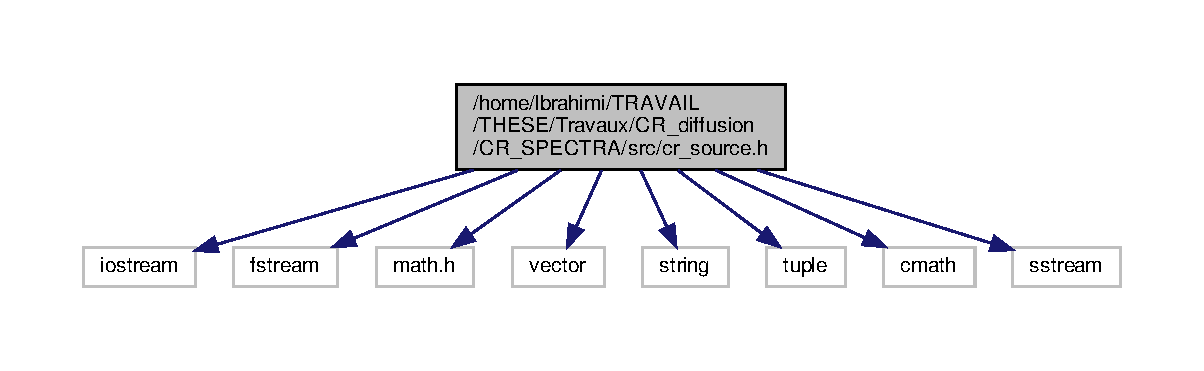
\includegraphics[width=350pt]{cr__source_8h__incl}
\end{center}
\end{figure}
This graph shows which files directly or indirectly include this file\+:\nopagebreak
\begin{figure}[H]
\begin{center}
\leavevmode
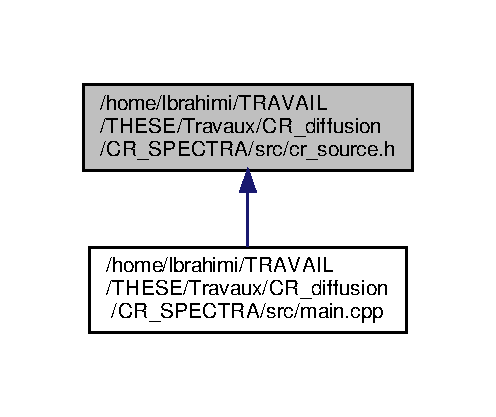
\includegraphics[width=238pt]{cr__source_8h__dep__incl}
\end{center}
\end{figure}
\subsection*{Functions}
\begin{DoxyCompactItemize}
\item 
double \hyperlink{cr__source_8h_a2fb2c7641ca839cbce7ea880f24ec761}{Get\+T\+Sed} ()
\item 
double \hyperlink{cr__source_8h_a9ae5a44cdfe05ba3ec18c58bb8a9acba}{R\+S\+NR} (double time)
\item 
double \hyperlink{cr__source_8h_adfcbd2247443f9569e3cb426495e4693}{u\+\_\+sh} (double time)
\begin{DoxyCompactList}\small\item\em Shock velocity in time. \end{DoxyCompactList}\item 
double \hyperlink{cr__source_8h_a120bb660287d2dcf66e013fb3925ce40}{Get\+EM} ()
\begin{DoxyCompactList}\small\item\em Get the E\+M\+AX value for the tesc calculation. \end{DoxyCompactList}\item 
double \hyperlink{cr__source_8h_aaddb8ae16ca149e0438df68d1a24496c}{tesc} (double E)
\item 
double \hyperlink{cr__source_8h_a893599c6c146a1fa4d5840dc503aa74b}{B\+\_\+sat} (double time)
\item 
double \hyperlink{cr__source_8h_ac1b13fc8cce3d466b305bc86f7406ef5}{Get\+E\+M\+\_\+e} ()
\item 
double \hyperlink{cr__source_8h_a57278a4dafd696d3c4dda8e860d28fd8}{tesc\+\_\+e} (double E)
\item 
double \hyperlink{cr__source_8h_ac022daf450a32a65533a945d8a3499f4}{Resc} (double E)
\begin{DoxyCompactList}\small\item\em This function return the value of the escape shock radius at a given energy of protons. \end{DoxyCompactList}\item 
double \hyperlink{cr__source_8h_a2ee3db01aff2917316c7bb0b13e72b44}{sigm} (double E, double ttesc)
\begin{DoxyCompactList}\small\item\em This function defines the variance of the time injection function Finj of C\+Rs. \end{DoxyCompactList}\item 
double \hyperlink{cr__source_8h_abcc0fcb1268d990ccf536d0f403f4105}{Finj} (double t, double dt, double E, double ttesc)
\begin{DoxyCompactList}\small\item\em C\+Rs time injection function. \end{DoxyCompactList}\item 
double \hyperlink{cr__source_8h_a91a3bf9ce71325c8a7cbd31d8c474bff}{theta} (double z, double t, double Rsnr)
\begin{DoxyCompactList}\small\item\em This function define the spatial shape of the C\+Rs distribution at a given time. \end{DoxyCompactList}\item 
double \hyperlink{cr__source_8h_a2bc06ab411fd01599de0b5a7fc9e59db}{d\+NdE} (double E)
\begin{DoxyCompactList}\small\item\em This function defines the injection spectrum of both electrons of protons escaping from the S\+NR. \end{DoxyCompactList}\item 
double \hyperlink{cr__source_8h_ab547f105d66b3ae0c64a2a49fdf4ca0d}{ff} (double E)
\begin{DoxyCompactList}\small\item\em This function defines the distribution function of both electrons and protrons escaping from the S\+NR. \end{DoxyCompactList}\item 
double \hyperlink{cr__source_8h_ac19e2251663c1020061917ef7c2ce4cb}{Pcr\+\_\+ini} (double E)
\begin{DoxyCompactList}\small\item\em This function defines the initial pressure distribution of both electrons and protons escaping from the S\+NR. \end{DoxyCompactList}\end{DoxyCompactItemize}
\subsection*{Variables}
\begin{DoxyCompactItemize}
\item 
std\+::string \hyperlink{cr__source_8h_ac41bf730655467ef90d688d783a49ce4}{parameters} = \char`\"{}./parameters.\+dat\char`\"{}
\item 
std\+::string \hyperlink{cr__source_8h_a9215c5392c20f3e08a28e47f8c4c181f}{snx} = \hyperlink{freader_8h_a073c1fd0247d9a7eb21c7a833eb3a2ad}{search}(\hyperlink{cr__source_8h_ac41bf730655467ef90d688d783a49ce4}{parameters}, \char`\"{}NX\char`\"{})
\item 
int \hyperlink{cr__source_8h_a02d47a4f36ec0bcce348696534567e30}{nx} = stoi(\hyperlink{cr__source_8h_a9215c5392c20f3e08a28e47f8c4c181f}{snx})
\item 
std\+::string \hyperlink{cr__source_8h_ac8b88baaf7ef9cabaeff4fe05d3f8faf}{sne} = \hyperlink{freader_8h_a073c1fd0247d9a7eb21c7a833eb3a2ad}{search}(\hyperlink{cr__source_8h_ac41bf730655467ef90d688d783a49ce4}{parameters}, \char`\"{}NE\char`\"{})
\item 
int \hyperlink{cr__source_8h_a3bf1137663f19e5c361c845cf4dfb7db}{ne} = stoi(\hyperlink{cr__source_8h_ac8b88baaf7ef9cabaeff4fe05d3f8faf}{sne})
\item 
std\+::string \hyperlink{cr__source_8h_a6dd5063f45011979396b374b20ebeb05}{sni} = \hyperlink{freader_8h_a073c1fd0247d9a7eb21c7a833eb3a2ad}{search}(\hyperlink{cr__source_8h_ac41bf730655467ef90d688d783a49ce4}{parameters},\char`\"{}ni\char`\"{})
\item 
double \hyperlink{cr__source_8h_ad3975adf480fdb09e1ea14b1efa617e0}{ni} = stod(\hyperlink{cr__source_8h_a6dd5063f45011979396b374b20ebeb05}{sni})
\item 
std\+::string \hyperlink{cr__source_8h_a24d54695f5ef59fa7003a6592ad2eb3e}{sX} = \hyperlink{freader_8h_a073c1fd0247d9a7eb21c7a833eb3a2ad}{search}(\hyperlink{cr__source_8h_ac41bf730655467ef90d688d783a49ce4}{parameters},\char`\"{}X\char`\"{})
\item 
double \hyperlink{cr__source_8h_a855d4a4ac47df1c46caacb1b42eb6d04}{Xi} = stod(\hyperlink{cr__source_8h_a24d54695f5ef59fa7003a6592ad2eb3e}{sX})
\item 
double \hyperlink{cr__source_8h_ad39423a7b14094ed17af35a0603f1a33}{nt} = \hyperlink{cr__source_8h_ad3975adf480fdb09e1ea14b1efa617e0}{ni}/\hyperlink{cr__source_8h_a855d4a4ac47df1c46caacb1b42eb6d04}{Xi}
\item 
std\+::string \hyperlink{cr__source_8h_ac763da942cab0e433e8187cfb5412905}{smn} = \hyperlink{freader_8h_a073c1fd0247d9a7eb21c7a833eb3a2ad}{search}(\hyperlink{cr__source_8h_ac41bf730655467ef90d688d783a49ce4}{parameters},\char`\"{}mn\char`\"{})
\item 
double \hyperlink{cr__source_8h_a86d5046913b91deb282e7c75c1e35acb}{m\+\_\+neutral} = stod(\hyperlink{cr__source_8h_ac763da942cab0e433e8187cfb5412905}{smn})
\item 
std\+::string \hyperlink{cr__source_8h_a4b33ff781b0ef1e9ed5a263c34bf7fe8}{sT} = \hyperlink{freader_8h_a073c1fd0247d9a7eb21c7a833eb3a2ad}{search}(\hyperlink{cr__source_8h_ac41bf730655467ef90d688d783a49ce4}{parameters},\char`\"{}T\char`\"{})
\item 
double \hyperlink{cr__source_8h_ac94a6e5794c2d7b59588b14025cfba20}{T} = stod(\hyperlink{cr__source_8h_a4b33ff781b0ef1e9ed5a263c34bf7fe8}{sT})
\item 
std\+::string \hyperlink{cr__source_8h_a131888f8169fa00af3616e4808fb6208}{scenter} = \hyperlink{freader_8h_a073c1fd0247d9a7eb21c7a833eb3a2ad}{search}(\hyperlink{cr__source_8h_ac41bf730655467ef90d688d783a49ce4}{parameters}, \char`\"{}center\char`\"{})
\item 
double \hyperlink{cr__source_8h_a655c95cafb81ec683d3e164a5eb2096d}{x\+\_\+center} = stod(\hyperlink{cr__source_8h_a131888f8169fa00af3616e4808fb6208}{scenter})
\item 
std\+::string \hyperlink{cr__source_8h_a7aeee0cbcc7af1970d2da3721b3fc9b9}{scenter\+\_\+index} = \hyperlink{freader_8h_a073c1fd0247d9a7eb21c7a833eb3a2ad}{search}(\hyperlink{cr__source_8h_ac41bf730655467ef90d688d783a49ce4}{parameters}, \char`\"{}center\+\_\+index\char`\"{})
\item 
int \hyperlink{cr__source_8h_a5445b70da42fff72267a9c8fa83531bc}{x\+\_\+center\+\_\+index} = stod(\hyperlink{cr__source_8h_a7aeee0cbcc7af1970d2da3721b3fc9b9}{scenter\+\_\+index})
\item 
std\+::string \hyperlink{cr__source_8h_a7d12f5e50e6da226a0a1bc433751d056}{s\+Bcenter} = \hyperlink{freader_8h_a073c1fd0247d9a7eb21c7a833eb3a2ad}{search}(\hyperlink{cr__source_8h_ac41bf730655467ef90d688d783a49ce4}{parameters}, \char`\"{}B\char`\"{})
\item 
double \hyperlink{cr__source_8h_acba2a7dbafb604d150d484cae70c8f3c}{Bcenter} = stod(\hyperlink{cr__source_8h_a7d12f5e50e6da226a0a1bc433751d056}{s\+Bcenter})
\end{DoxyCompactItemize}


\subsection{Function Documentation}
\mbox{\Hypertarget{cr__source_8h_a893599c6c146a1fa4d5840dc503aa74b}\label{cr__source_8h_a893599c6c146a1fa4d5840dc503aa74b}} 
\index{cr\+\_\+source.\+h@{cr\+\_\+source.\+h}!B\+\_\+sat@{B\+\_\+sat}}
\index{B\+\_\+sat@{B\+\_\+sat}!cr\+\_\+source.\+h@{cr\+\_\+source.\+h}}
\subsubsection{\texorpdfstring{B\+\_\+sat()}{B\_sat()}}
{\footnotesize\ttfamily double B\+\_\+sat (\begin{DoxyParamCaption}\item[{double}]{time }\end{DoxyParamCaption})}

\mbox{\Hypertarget{cr__source_8h_a2bc06ab411fd01599de0b5a7fc9e59db}\label{cr__source_8h_a2bc06ab411fd01599de0b5a7fc9e59db}} 
\index{cr\+\_\+source.\+h@{cr\+\_\+source.\+h}!d\+NdE@{d\+NdE}}
\index{d\+NdE@{d\+NdE}!cr\+\_\+source.\+h@{cr\+\_\+source.\+h}}
\subsubsection{\texorpdfstring{d\+Nd\+E()}{dNdE()}}
{\footnotesize\ttfamily double d\+NdE (\begin{DoxyParamCaption}\item[{double}]{E }\end{DoxyParamCaption})}



This function defines the injection spectrum of both electrons of protons escaping from the S\+NR. 

\mbox{\Hypertarget{cr__source_8h_ab547f105d66b3ae0c64a2a49fdf4ca0d}\label{cr__source_8h_ab547f105d66b3ae0c64a2a49fdf4ca0d}} 
\index{cr\+\_\+source.\+h@{cr\+\_\+source.\+h}!ff@{ff}}
\index{ff@{ff}!cr\+\_\+source.\+h@{cr\+\_\+source.\+h}}
\subsubsection{\texorpdfstring{ff()}{ff()}}
{\footnotesize\ttfamily double ff (\begin{DoxyParamCaption}\item[{double}]{E }\end{DoxyParamCaption})}



This function defines the distribution function of both electrons and protrons escaping from the S\+NR. 

\mbox{\Hypertarget{cr__source_8h_abcc0fcb1268d990ccf536d0f403f4105}\label{cr__source_8h_abcc0fcb1268d990ccf536d0f403f4105}} 
\index{cr\+\_\+source.\+h@{cr\+\_\+source.\+h}!Finj@{Finj}}
\index{Finj@{Finj}!cr\+\_\+source.\+h@{cr\+\_\+source.\+h}}
\subsubsection{\texorpdfstring{Finj()}{Finj()}}
{\footnotesize\ttfamily double Finj (\begin{DoxyParamCaption}\item[{double}]{t,  }\item[{double}]{dt,  }\item[{double}]{E,  }\item[{double}]{ttesc }\end{DoxyParamCaption})}



C\+Rs time injection function. 

\mbox{\Hypertarget{cr__source_8h_a120bb660287d2dcf66e013fb3925ce40}\label{cr__source_8h_a120bb660287d2dcf66e013fb3925ce40}} 
\index{cr\+\_\+source.\+h@{cr\+\_\+source.\+h}!Get\+EM@{Get\+EM}}
\index{Get\+EM@{Get\+EM}!cr\+\_\+source.\+h@{cr\+\_\+source.\+h}}
\subsubsection{\texorpdfstring{Get\+E\+M()}{GetEM()}}
{\footnotesize\ttfamily double Get\+EM (\begin{DoxyParamCaption}{ }\end{DoxyParamCaption})}



Get the E\+M\+AX value for the tesc calculation. 

\mbox{\Hypertarget{cr__source_8h_ac1b13fc8cce3d466b305bc86f7406ef5}\label{cr__source_8h_ac1b13fc8cce3d466b305bc86f7406ef5}} 
\index{cr\+\_\+source.\+h@{cr\+\_\+source.\+h}!Get\+E\+M\+\_\+e@{Get\+E\+M\+\_\+e}}
\index{Get\+E\+M\+\_\+e@{Get\+E\+M\+\_\+e}!cr\+\_\+source.\+h@{cr\+\_\+source.\+h}}
\subsubsection{\texorpdfstring{Get\+E\+M\+\_\+e()}{GetEM\_e()}}
{\footnotesize\ttfamily double Get\+E\+M\+\_\+e (\begin{DoxyParamCaption}{ }\end{DoxyParamCaption})}

This function allows to calculate the maximum energy provided to the electrons escaping from the S\+NR according to the values in the constans.\+h file. \mbox{\Hypertarget{cr__source_8h_a2fb2c7641ca839cbce7ea880f24ec761}\label{cr__source_8h_a2fb2c7641ca839cbce7ea880f24ec761}} 
\index{cr\+\_\+source.\+h@{cr\+\_\+source.\+h}!Get\+T\+Sed@{Get\+T\+Sed}}
\index{Get\+T\+Sed@{Get\+T\+Sed}!cr\+\_\+source.\+h@{cr\+\_\+source.\+h}}
\subsubsection{\texorpdfstring{Get\+T\+Sed()}{GetTSed()}}
{\footnotesize\ttfamily double Get\+T\+Sed (\begin{DoxyParamCaption}{ }\end{DoxyParamCaption})}

This function return the value of t\+\_\+sedov according to the S\+NR properties specified in the \hyperlink{constants_8h}{constants.\+h} file \mbox{\Hypertarget{cr__source_8h_ac19e2251663c1020061917ef7c2ce4cb}\label{cr__source_8h_ac19e2251663c1020061917ef7c2ce4cb}} 
\index{cr\+\_\+source.\+h@{cr\+\_\+source.\+h}!Pcr\+\_\+ini@{Pcr\+\_\+ini}}
\index{Pcr\+\_\+ini@{Pcr\+\_\+ini}!cr\+\_\+source.\+h@{cr\+\_\+source.\+h}}
\subsubsection{\texorpdfstring{Pcr\+\_\+ini()}{Pcr\_ini()}}
{\footnotesize\ttfamily double Pcr\+\_\+ini (\begin{DoxyParamCaption}\item[{double}]{E }\end{DoxyParamCaption})}



This function defines the initial pressure distribution of both electrons and protons escaping from the S\+NR. 

\mbox{\Hypertarget{cr__source_8h_ac022daf450a32a65533a945d8a3499f4}\label{cr__source_8h_ac022daf450a32a65533a945d8a3499f4}} 
\index{cr\+\_\+source.\+h@{cr\+\_\+source.\+h}!Resc@{Resc}}
\index{Resc@{Resc}!cr\+\_\+source.\+h@{cr\+\_\+source.\+h}}
\subsubsection{\texorpdfstring{Resc()}{Resc()}}
{\footnotesize\ttfamily double Resc (\begin{DoxyParamCaption}\item[{double}]{E }\end{DoxyParamCaption})}



This function return the value of the escape shock radius at a given energy of protons. 

\mbox{\Hypertarget{cr__source_8h_a9ae5a44cdfe05ba3ec18c58bb8a9acba}\label{cr__source_8h_a9ae5a44cdfe05ba3ec18c58bb8a9acba}} 
\index{cr\+\_\+source.\+h@{cr\+\_\+source.\+h}!R\+S\+NR@{R\+S\+NR}}
\index{R\+S\+NR@{R\+S\+NR}!cr\+\_\+source.\+h@{cr\+\_\+source.\+h}}
\subsubsection{\texorpdfstring{R\+S\+N\+R()}{RSNR()}}
{\footnotesize\ttfamily double R\+S\+NR (\begin{DoxyParamCaption}\item[{double}]{time }\end{DoxyParamCaption})}

This function provides the value of the shock radius as a function of the time according to the S\+NR expansion model from Cioffi et al. 1998 and Truelove \& Mc\+Kee 19... The S\+NR shock has different propagation stages which are separated by characteristic times defined as below \+: \begin{eqnarray*} t_{\mathrm{ini},\mathrm{kyr}} & = & 10^{-4} \\ t_{\mathrm{free}, \mathrm{kyr}} & = & 0.3 E_\mathrm{SN}^{-1/2} M_\mathrm{ej} n_t^{-1/3} \\ t_{\mathrm{PDS}, \mathrm{yr}} & = & e^{-1} \times 3.61 \times 10^4 E_\mathrm{SN}^{3/14}/(\xi_n^{5/14}n_t^{4/7}) \\ t_{\mathrm{MCS}, \mathrm{yr}} & = & \mathrm{min}\left[ 61 V_{\mathrm{ej},8}^3/(\xi_n^{9/14}*n_t^{3/7}*E_\mathrm{SN}^{3/14}), 476 t_{\mathrm{PDS}, \mathrm{yr}} / (\xi_n \phi_c)^{9/14} \right] \\ t_{\mathrm{merge}, \mathrm{yr}} & = & 153 \left(E_\mathrm{SN}^{1/14} n_t^{1/7} \xi_n^{3/14}/ (\beta C_{06}) \right)^{10/7} t_{\mathrm{PDS}, \mathrm{yr}} \\ t_\mathrm{max} & = & \mathrm{max}(t_\mathrm{MCS}, t_\mathrm{merge}) \end{eqnarray*} where $ t_\mathrm{ini}$ corresponds to the initial time of the numerical computation of the spline, $ t_\mathrm{free} $ correponds to the transition time between the free expansion phase and the Sedov-\/\+Taylor phase, $ t_\mathrm{PDS} $ corresponds to the transition time between the Sedov-\/\+Taylor phase and the Pressure Driven Snowplow phase, $ t_\mathrm{MCS} $ correponds to the transition time between the Pressure Driven Snowplow phase and the Momentum Conserving Snowplow phase and finally $ t_\mathrm{merge} $ means the time at which the shock pressure becomes of the order of the I\+SM pressure. In some I\+SM phases, the shock can merge before entering in the Momentum Conserving Snowplow phase explaining $ t_\mathrm{max} $. The S\+NR shock evolves with time according the following radii \begin{eqnarray*} R_\mathrm{ini} & = & R_\mathrm{free} (t_\mathrm{ini}/t_\mathrm{free}) \\ \end{eqnarray*}


\begin{DoxyParams}{Parameters}
{\em time} & Time in \mbox{[}s\mbox{]}. \\
\hline
\end{DoxyParams}
\begin{DoxySeeAlso}{See also}
\hyperlink{cr__source_8h_a9ae5a44cdfe05ba3ec18c58bb8a9acba}{R\+S\+N\+R()}, \hyperlink{mathematics_8h_aa9efdc9b8bb19a51263aef089b14a129}{Interpolating\+Spline()}
\end{DoxySeeAlso}
\mbox{\Hypertarget{cr__source_8h_a2ee3db01aff2917316c7bb0b13e72b44}\label{cr__source_8h_a2ee3db01aff2917316c7bb0b13e72b44}} 
\index{cr\+\_\+source.\+h@{cr\+\_\+source.\+h}!sigm@{sigm}}
\index{sigm@{sigm}!cr\+\_\+source.\+h@{cr\+\_\+source.\+h}}
\subsubsection{\texorpdfstring{sigm()}{sigm()}}
{\footnotesize\ttfamily double sigm (\begin{DoxyParamCaption}\item[{double}]{E,  }\item[{double}]{ttesc }\end{DoxyParamCaption})}



This function defines the variance of the time injection function Finj of C\+Rs. 

\mbox{\Hypertarget{cr__source_8h_aaddb8ae16ca149e0438df68d1a24496c}\label{cr__source_8h_aaddb8ae16ca149e0438df68d1a24496c}} 
\index{cr\+\_\+source.\+h@{cr\+\_\+source.\+h}!tesc@{tesc}}
\index{tesc@{tesc}!cr\+\_\+source.\+h@{cr\+\_\+source.\+h}}
\subsubsection{\texorpdfstring{tesc()}{tesc()}}
{\footnotesize\ttfamily double tesc (\begin{DoxyParamCaption}\item[{double}]{E }\end{DoxyParamCaption})}

Protons escape time function according the model of Celli et al. (2019) but also alternatives models of CR escape during radiative stages \mbox{\Hypertarget{cr__source_8h_a57278a4dafd696d3c4dda8e860d28fd8}\label{cr__source_8h_a57278a4dafd696d3c4dda8e860d28fd8}} 
\index{cr\+\_\+source.\+h@{cr\+\_\+source.\+h}!tesc\+\_\+e@{tesc\+\_\+e}}
\index{tesc\+\_\+e@{tesc\+\_\+e}!cr\+\_\+source.\+h@{cr\+\_\+source.\+h}}
\subsubsection{\texorpdfstring{tesc\+\_\+e()}{tesc\_e()}}
{\footnotesize\ttfamily double tesc\+\_\+e (\begin{DoxyParamCaption}\item[{double}]{E }\end{DoxyParamCaption})}

This function calulate the escape time of the electrons as a function of the energy according both model of escape from Celli et al. (2019) and alternative models of escape in radiative phases \mbox{\Hypertarget{cr__source_8h_a91a3bf9ce71325c8a7cbd31d8c474bff}\label{cr__source_8h_a91a3bf9ce71325c8a7cbd31d8c474bff}} 
\index{cr\+\_\+source.\+h@{cr\+\_\+source.\+h}!theta@{theta}}
\index{theta@{theta}!cr\+\_\+source.\+h@{cr\+\_\+source.\+h}}
\subsubsection{\texorpdfstring{theta()}{theta()}}
{\footnotesize\ttfamily double theta (\begin{DoxyParamCaption}\item[{double}]{z,  }\item[{double}]{t,  }\item[{double}]{Rsnr }\end{DoxyParamCaption})}



This function define the spatial shape of the C\+Rs distribution at a given time. 

\mbox{\Hypertarget{cr__source_8h_adfcbd2247443f9569e3cb426495e4693}\label{cr__source_8h_adfcbd2247443f9569e3cb426495e4693}} 
\index{cr\+\_\+source.\+h@{cr\+\_\+source.\+h}!u\+\_\+sh@{u\+\_\+sh}}
\index{u\+\_\+sh@{u\+\_\+sh}!cr\+\_\+source.\+h@{cr\+\_\+source.\+h}}
\subsubsection{\texorpdfstring{u\+\_\+sh()}{u\_sh()}}
{\footnotesize\ttfamily double u\+\_\+sh (\begin{DoxyParamCaption}\item[{double}]{time }\end{DoxyParamCaption})}



Shock velocity in time. 



\subsection{Variable Documentation}
\mbox{\Hypertarget{cr__source_8h_acba2a7dbafb604d150d484cae70c8f3c}\label{cr__source_8h_acba2a7dbafb604d150d484cae70c8f3c}} 
\index{cr\+\_\+source.\+h@{cr\+\_\+source.\+h}!Bcenter@{Bcenter}}
\index{Bcenter@{Bcenter}!cr\+\_\+source.\+h@{cr\+\_\+source.\+h}}
\subsubsection{\texorpdfstring{Bcenter}{Bcenter}}
{\footnotesize\ttfamily double Bcenter = stod(\hyperlink{cr__source_8h_a7d12f5e50e6da226a0a1bc433751d056}{s\+Bcenter})}

\mbox{\Hypertarget{cr__source_8h_a86d5046913b91deb282e7c75c1e35acb}\label{cr__source_8h_a86d5046913b91deb282e7c75c1e35acb}} 
\index{cr\+\_\+source.\+h@{cr\+\_\+source.\+h}!m\+\_\+neutral@{m\+\_\+neutral}}
\index{m\+\_\+neutral@{m\+\_\+neutral}!cr\+\_\+source.\+h@{cr\+\_\+source.\+h}}
\subsubsection{\texorpdfstring{m\+\_\+neutral}{m\_neutral}}
{\footnotesize\ttfamily double m\+\_\+neutral = stod(\hyperlink{cr__source_8h_ac763da942cab0e433e8187cfb5412905}{smn})}

\mbox{\Hypertarget{cr__source_8h_a3bf1137663f19e5c361c845cf4dfb7db}\label{cr__source_8h_a3bf1137663f19e5c361c845cf4dfb7db}} 
\index{cr\+\_\+source.\+h@{cr\+\_\+source.\+h}!ne@{ne}}
\index{ne@{ne}!cr\+\_\+source.\+h@{cr\+\_\+source.\+h}}
\subsubsection{\texorpdfstring{ne}{ne}}
{\footnotesize\ttfamily int ne = stoi(\hyperlink{cr__source_8h_ac8b88baaf7ef9cabaeff4fe05d3f8faf}{sne})}

\mbox{\Hypertarget{cr__source_8h_ad3975adf480fdb09e1ea14b1efa617e0}\label{cr__source_8h_ad3975adf480fdb09e1ea14b1efa617e0}} 
\index{cr\+\_\+source.\+h@{cr\+\_\+source.\+h}!ni@{ni}}
\index{ni@{ni}!cr\+\_\+source.\+h@{cr\+\_\+source.\+h}}
\subsubsection{\texorpdfstring{ni}{ni}}
{\footnotesize\ttfamily double ni = stod(\hyperlink{cr__source_8h_a6dd5063f45011979396b374b20ebeb05}{sni})}

\mbox{\Hypertarget{cr__source_8h_ad39423a7b14094ed17af35a0603f1a33}\label{cr__source_8h_ad39423a7b14094ed17af35a0603f1a33}} 
\index{cr\+\_\+source.\+h@{cr\+\_\+source.\+h}!nt@{nt}}
\index{nt@{nt}!cr\+\_\+source.\+h@{cr\+\_\+source.\+h}}
\subsubsection{\texorpdfstring{nt}{nt}}
{\footnotesize\ttfamily double nt = \hyperlink{cr__source_8h_ad3975adf480fdb09e1ea14b1efa617e0}{ni}/\hyperlink{cr__source_8h_a855d4a4ac47df1c46caacb1b42eb6d04}{Xi}}

\mbox{\Hypertarget{cr__source_8h_a02d47a4f36ec0bcce348696534567e30}\label{cr__source_8h_a02d47a4f36ec0bcce348696534567e30}} 
\index{cr\+\_\+source.\+h@{cr\+\_\+source.\+h}!nx@{nx}}
\index{nx@{nx}!cr\+\_\+source.\+h@{cr\+\_\+source.\+h}}
\subsubsection{\texorpdfstring{nx}{nx}}
{\footnotesize\ttfamily int nx = stoi(\hyperlink{cr__source_8h_a9215c5392c20f3e08a28e47f8c4c181f}{snx})}

\mbox{\Hypertarget{cr__source_8h_ac41bf730655467ef90d688d783a49ce4}\label{cr__source_8h_ac41bf730655467ef90d688d783a49ce4}} 
\index{cr\+\_\+source.\+h@{cr\+\_\+source.\+h}!parameters@{parameters}}
\index{parameters@{parameters}!cr\+\_\+source.\+h@{cr\+\_\+source.\+h}}
\subsubsection{\texorpdfstring{parameters}{parameters}}
{\footnotesize\ttfamily std\+::string parameters = \char`\"{}./parameters.\+dat\char`\"{}}

\mbox{\Hypertarget{cr__source_8h_a7d12f5e50e6da226a0a1bc433751d056}\label{cr__source_8h_a7d12f5e50e6da226a0a1bc433751d056}} 
\index{cr\+\_\+source.\+h@{cr\+\_\+source.\+h}!s\+Bcenter@{s\+Bcenter}}
\index{s\+Bcenter@{s\+Bcenter}!cr\+\_\+source.\+h@{cr\+\_\+source.\+h}}
\subsubsection{\texorpdfstring{s\+Bcenter}{sBcenter}}
{\footnotesize\ttfamily std\+::string s\+Bcenter = \hyperlink{freader_8h_a073c1fd0247d9a7eb21c7a833eb3a2ad}{search}(\hyperlink{cr__source_8h_ac41bf730655467ef90d688d783a49ce4}{parameters}, \char`\"{}B\char`\"{})}

\mbox{\Hypertarget{cr__source_8h_a131888f8169fa00af3616e4808fb6208}\label{cr__source_8h_a131888f8169fa00af3616e4808fb6208}} 
\index{cr\+\_\+source.\+h@{cr\+\_\+source.\+h}!scenter@{scenter}}
\index{scenter@{scenter}!cr\+\_\+source.\+h@{cr\+\_\+source.\+h}}
\subsubsection{\texorpdfstring{scenter}{scenter}}
{\footnotesize\ttfamily std\+::string scenter = \hyperlink{freader_8h_a073c1fd0247d9a7eb21c7a833eb3a2ad}{search}(\hyperlink{cr__source_8h_ac41bf730655467ef90d688d783a49ce4}{parameters}, \char`\"{}center\char`\"{})}

\mbox{\Hypertarget{cr__source_8h_a7aeee0cbcc7af1970d2da3721b3fc9b9}\label{cr__source_8h_a7aeee0cbcc7af1970d2da3721b3fc9b9}} 
\index{cr\+\_\+source.\+h@{cr\+\_\+source.\+h}!scenter\+\_\+index@{scenter\+\_\+index}}
\index{scenter\+\_\+index@{scenter\+\_\+index}!cr\+\_\+source.\+h@{cr\+\_\+source.\+h}}
\subsubsection{\texorpdfstring{scenter\+\_\+index}{scenter\_index}}
{\footnotesize\ttfamily std\+::string scenter\+\_\+index = \hyperlink{freader_8h_a073c1fd0247d9a7eb21c7a833eb3a2ad}{search}(\hyperlink{cr__source_8h_ac41bf730655467ef90d688d783a49ce4}{parameters}, \char`\"{}center\+\_\+index\char`\"{})}

\mbox{\Hypertarget{cr__source_8h_ac763da942cab0e433e8187cfb5412905}\label{cr__source_8h_ac763da942cab0e433e8187cfb5412905}} 
\index{cr\+\_\+source.\+h@{cr\+\_\+source.\+h}!smn@{smn}}
\index{smn@{smn}!cr\+\_\+source.\+h@{cr\+\_\+source.\+h}}
\subsubsection{\texorpdfstring{smn}{smn}}
{\footnotesize\ttfamily std\+::string smn = \hyperlink{freader_8h_a073c1fd0247d9a7eb21c7a833eb3a2ad}{search}(\hyperlink{cr__source_8h_ac41bf730655467ef90d688d783a49ce4}{parameters},\char`\"{}mn\char`\"{})}

\mbox{\Hypertarget{cr__source_8h_ac8b88baaf7ef9cabaeff4fe05d3f8faf}\label{cr__source_8h_ac8b88baaf7ef9cabaeff4fe05d3f8faf}} 
\index{cr\+\_\+source.\+h@{cr\+\_\+source.\+h}!sne@{sne}}
\index{sne@{sne}!cr\+\_\+source.\+h@{cr\+\_\+source.\+h}}
\subsubsection{\texorpdfstring{sne}{sne}}
{\footnotesize\ttfamily std\+::string sne = \hyperlink{freader_8h_a073c1fd0247d9a7eb21c7a833eb3a2ad}{search}(\hyperlink{cr__source_8h_ac41bf730655467ef90d688d783a49ce4}{parameters}, \char`\"{}NE\char`\"{})}

\mbox{\Hypertarget{cr__source_8h_a6dd5063f45011979396b374b20ebeb05}\label{cr__source_8h_a6dd5063f45011979396b374b20ebeb05}} 
\index{cr\+\_\+source.\+h@{cr\+\_\+source.\+h}!sni@{sni}}
\index{sni@{sni}!cr\+\_\+source.\+h@{cr\+\_\+source.\+h}}
\subsubsection{\texorpdfstring{sni}{sni}}
{\footnotesize\ttfamily std\+::string sni = \hyperlink{freader_8h_a073c1fd0247d9a7eb21c7a833eb3a2ad}{search}(\hyperlink{cr__source_8h_ac41bf730655467ef90d688d783a49ce4}{parameters},\char`\"{}ni\char`\"{})}

\mbox{\Hypertarget{cr__source_8h_a9215c5392c20f3e08a28e47f8c4c181f}\label{cr__source_8h_a9215c5392c20f3e08a28e47f8c4c181f}} 
\index{cr\+\_\+source.\+h@{cr\+\_\+source.\+h}!snx@{snx}}
\index{snx@{snx}!cr\+\_\+source.\+h@{cr\+\_\+source.\+h}}
\subsubsection{\texorpdfstring{snx}{snx}}
{\footnotesize\ttfamily std\+::string snx = \hyperlink{freader_8h_a073c1fd0247d9a7eb21c7a833eb3a2ad}{search}(\hyperlink{cr__source_8h_ac41bf730655467ef90d688d783a49ce4}{parameters}, \char`\"{}NX\char`\"{})}

\mbox{\Hypertarget{cr__source_8h_a4b33ff781b0ef1e9ed5a263c34bf7fe8}\label{cr__source_8h_a4b33ff781b0ef1e9ed5a263c34bf7fe8}} 
\index{cr\+\_\+source.\+h@{cr\+\_\+source.\+h}!sT@{sT}}
\index{sT@{sT}!cr\+\_\+source.\+h@{cr\+\_\+source.\+h}}
\subsubsection{\texorpdfstring{sT}{sT}}
{\footnotesize\ttfamily std\+::string sT = \hyperlink{freader_8h_a073c1fd0247d9a7eb21c7a833eb3a2ad}{search}(\hyperlink{cr__source_8h_ac41bf730655467ef90d688d783a49ce4}{parameters},\char`\"{}T\char`\"{})}

\mbox{\Hypertarget{cr__source_8h_a24d54695f5ef59fa7003a6592ad2eb3e}\label{cr__source_8h_a24d54695f5ef59fa7003a6592ad2eb3e}} 
\index{cr\+\_\+source.\+h@{cr\+\_\+source.\+h}!sX@{sX}}
\index{sX@{sX}!cr\+\_\+source.\+h@{cr\+\_\+source.\+h}}
\subsubsection{\texorpdfstring{sX}{sX}}
{\footnotesize\ttfamily std\+::string sX = \hyperlink{freader_8h_a073c1fd0247d9a7eb21c7a833eb3a2ad}{search}(\hyperlink{cr__source_8h_ac41bf730655467ef90d688d783a49ce4}{parameters},\char`\"{}X\char`\"{})}

\mbox{\Hypertarget{cr__source_8h_ac94a6e5794c2d7b59588b14025cfba20}\label{cr__source_8h_ac94a6e5794c2d7b59588b14025cfba20}} 
\index{cr\+\_\+source.\+h@{cr\+\_\+source.\+h}!T@{T}}
\index{T@{T}!cr\+\_\+source.\+h@{cr\+\_\+source.\+h}}
\subsubsection{\texorpdfstring{T}{T}}
{\footnotesize\ttfamily double T = stod(\hyperlink{cr__source_8h_a4b33ff781b0ef1e9ed5a263c34bf7fe8}{sT})}

\mbox{\Hypertarget{cr__source_8h_a655c95cafb81ec683d3e164a5eb2096d}\label{cr__source_8h_a655c95cafb81ec683d3e164a5eb2096d}} 
\index{cr\+\_\+source.\+h@{cr\+\_\+source.\+h}!x\+\_\+center@{x\+\_\+center}}
\index{x\+\_\+center@{x\+\_\+center}!cr\+\_\+source.\+h@{cr\+\_\+source.\+h}}
\subsubsection{\texorpdfstring{x\+\_\+center}{x\_center}}
{\footnotesize\ttfamily double x\+\_\+center = stod(\hyperlink{cr__source_8h_a131888f8169fa00af3616e4808fb6208}{scenter})}

\mbox{\Hypertarget{cr__source_8h_a5445b70da42fff72267a9c8fa83531bc}\label{cr__source_8h_a5445b70da42fff72267a9c8fa83531bc}} 
\index{cr\+\_\+source.\+h@{cr\+\_\+source.\+h}!x\+\_\+center\+\_\+index@{x\+\_\+center\+\_\+index}}
\index{x\+\_\+center\+\_\+index@{x\+\_\+center\+\_\+index}!cr\+\_\+source.\+h@{cr\+\_\+source.\+h}}
\subsubsection{\texorpdfstring{x\+\_\+center\+\_\+index}{x\_center\_index}}
{\footnotesize\ttfamily int x\+\_\+center\+\_\+index = stod(\hyperlink{cr__source_8h_a7aeee0cbcc7af1970d2da3721b3fc9b9}{scenter\+\_\+index})}

\mbox{\Hypertarget{cr__source_8h_a855d4a4ac47df1c46caacb1b42eb6d04}\label{cr__source_8h_a855d4a4ac47df1c46caacb1b42eb6d04}} 
\index{cr\+\_\+source.\+h@{cr\+\_\+source.\+h}!Xi@{Xi}}
\index{Xi@{Xi}!cr\+\_\+source.\+h@{cr\+\_\+source.\+h}}
\subsubsection{\texorpdfstring{Xi}{Xi}}
{\footnotesize\ttfamily double Xi = stod(\hyperlink{cr__source_8h_a24d54695f5ef59fa7003a6592ad2eb3e}{sX})}


\hypertarget{freader_8h}{}\section{/home/lbrahimi/\+T\+R\+A\+V\+A\+I\+L/\+T\+H\+E\+S\+E/\+Travaux/\+C\+R\+\_\+diffusion/\+C\+R\+\_\+\+S\+P\+E\+C\+T\+R\+A/src/freader.h File Reference}
\label{freader_8h}\index{/home/lbrahimi/\+T\+R\+A\+V\+A\+I\+L/\+T\+H\+E\+S\+E/\+Travaux/\+C\+R\+\_\+diffusion/\+C\+R\+\_\+\+S\+P\+E\+C\+T\+R\+A/src/freader.\+h@{/home/lbrahimi/\+T\+R\+A\+V\+A\+I\+L/\+T\+H\+E\+S\+E/\+Travaux/\+C\+R\+\_\+diffusion/\+C\+R\+\_\+\+S\+P\+E\+C\+T\+R\+A/src/freader.\+h}}
{\ttfamily \#include $<$iostream$>$}\newline
{\ttfamily \#include $<$fstream$>$}\newline
{\ttfamily \#include $<$math.\+h$>$}\newline
{\ttfamily \#include $<$vector$>$}\newline
{\ttfamily \#include $<$string$>$}\newline
{\ttfamily \#include $<$tuple$>$}\newline
{\ttfamily \#include $<$cmath$>$}\newline
{\ttfamily \#include $<$sstream$>$}\newline
Include dependency graph for freader.\+h\+:\nopagebreak
\begin{figure}[H]
\begin{center}
\leavevmode
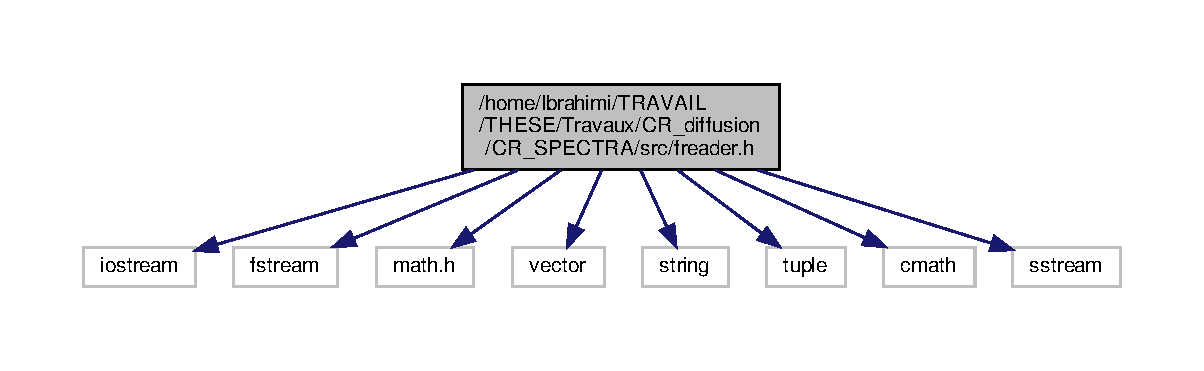
\includegraphics[width=350pt]{freader_8h__incl}
\end{center}
\end{figure}
This graph shows which files directly or indirectly include this file\+:\nopagebreak
\begin{figure}[H]
\begin{center}
\leavevmode
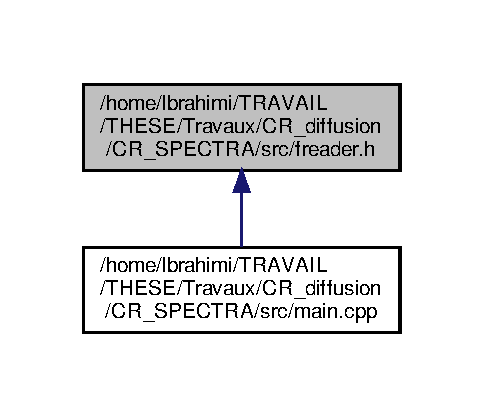
\includegraphics[width=232pt]{freader_8h__dep__incl}
\end{center}
\end{figure}
\subsection*{Functions}
\begin{DoxyCompactItemize}
\item 
std\+::string \hyperlink{freader_8h_a073c1fd0247d9a7eb21c7a833eb3a2ad}{search} (string file\+\_\+name, string variable)
\item 
vector$<$ double $>$ \hyperlink{freader_8h_a232e9971c42cf166f2ef866f35537edc}{read\+Axis} (std\+::string filename, int vec\+\_\+size)
\end{DoxyCompactItemize}


\subsection{Function Documentation}
\mbox{\Hypertarget{freader_8h_a232e9971c42cf166f2ef866f35537edc}\label{freader_8h_a232e9971c42cf166f2ef866f35537edc}} 
\index{freader.\+h@{freader.\+h}!read\+Axis@{read\+Axis}}
\index{read\+Axis@{read\+Axis}!freader.\+h@{freader.\+h}}
\subsubsection{\texorpdfstring{read\+Axis()}{readAxis()}}
{\footnotesize\ttfamily vector$<$double$>$ read\+Axis (\begin{DoxyParamCaption}\item[{std\+::string}]{filename,  }\item[{int}]{vec\+\_\+size }\end{DoxyParamCaption})}

\mbox{\Hypertarget{freader_8h_a073c1fd0247d9a7eb21c7a833eb3a2ad}\label{freader_8h_a073c1fd0247d9a7eb21c7a833eb3a2ad}} 
\index{freader.\+h@{freader.\+h}!search@{search}}
\index{search@{search}!freader.\+h@{freader.\+h}}
\subsubsection{\texorpdfstring{search()}{search()}}
{\footnotesize\ttfamily std\+::string search (\begin{DoxyParamCaption}\item[{string}]{file\+\_\+name,  }\item[{string}]{variable }\end{DoxyParamCaption})}


\hypertarget{fwritter_8h}{}\section{/home/lbrahimi/\+T\+R\+A\+V\+A\+I\+L/\+T\+H\+E\+S\+E/\+Travaux/\+C\+R\+\_\+diffusion/\+C\+R\+\_\+\+S\+P\+E\+C\+T\+R\+A/src/fwritter.h File Reference}
\label{fwritter_8h}\index{/home/lbrahimi/\+T\+R\+A\+V\+A\+I\+L/\+T\+H\+E\+S\+E/\+Travaux/\+C\+R\+\_\+diffusion/\+C\+R\+\_\+\+S\+P\+E\+C\+T\+R\+A/src/fwritter.\+h@{/home/lbrahimi/\+T\+R\+A\+V\+A\+I\+L/\+T\+H\+E\+S\+E/\+Travaux/\+C\+R\+\_\+diffusion/\+C\+R\+\_\+\+S\+P\+E\+C\+T\+R\+A/src/fwritter.\+h}}
{\ttfamily \#include $<$iostream$>$}\newline
{\ttfamily \#include $<$fstream$>$}\newline
{\ttfamily \#include $<$math.\+h$>$}\newline
{\ttfamily \#include $<$vector$>$}\newline
{\ttfamily \#include $<$string$>$}\newline
{\ttfamily \#include $<$tuple$>$}\newline
{\ttfamily \#include $<$cmath$>$}\newline
{\ttfamily \#include $<$sstream$>$}\newline
Include dependency graph for fwritter.\+h\+:\nopagebreak
\begin{figure}[H]
\begin{center}
\leavevmode
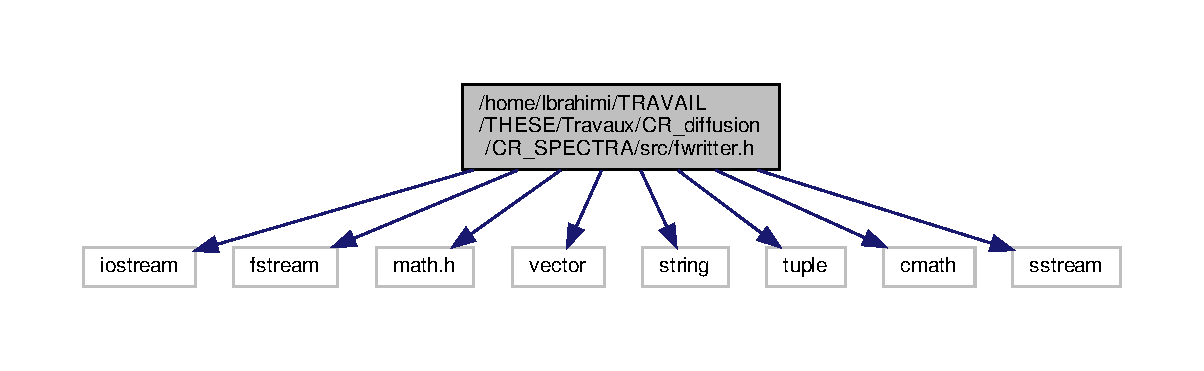
\includegraphics[width=350pt]{fwritter_8h__incl}
\end{center}
\end{figure}
This graph shows which files directly or indirectly include this file\+:\nopagebreak
\begin{figure}[H]
\begin{center}
\leavevmode
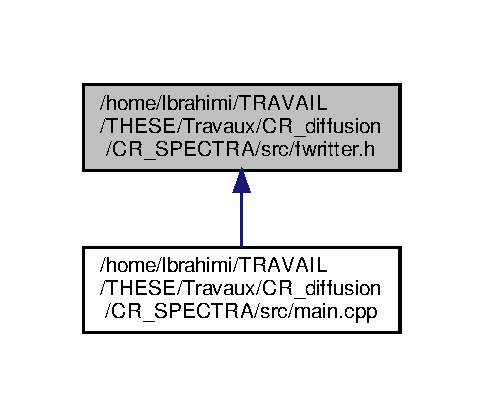
\includegraphics[width=232pt]{fwritter_8h__dep__incl}
\end{center}
\end{figure}
\subsection*{Functions}
\begin{DoxyCompactItemize}
\item 
int \hyperlink{fwritter_8h_afc1fc2295f604e69d406f6cfd8cabcd9}{write\+XE} (std\+::string filename, int index, vector$<$ vector$<$ double $>$ $>$ data, double NX, double NE)
\item 
int \hyperlink{fwritter_8h_ab16a679770c5287ffdf40d8f19319c36}{write\+Info} (std\+::string filename, int index, vector$<$ double $>$ info, vector$<$ std\+::string $>$ s\+\_\+info)
\end{DoxyCompactItemize}


\subsection{Function Documentation}
\mbox{\Hypertarget{fwritter_8h_ab16a679770c5287ffdf40d8f19319c36}\label{fwritter_8h_ab16a679770c5287ffdf40d8f19319c36}} 
\index{fwritter.\+h@{fwritter.\+h}!write\+Info@{write\+Info}}
\index{write\+Info@{write\+Info}!fwritter.\+h@{fwritter.\+h}}
\subsubsection{\texorpdfstring{write\+Info()}{writeInfo()}}
{\footnotesize\ttfamily int write\+Info (\begin{DoxyParamCaption}\item[{std\+::string}]{filename,  }\item[{int}]{index,  }\item[{vector$<$ double $>$}]{info,  }\item[{vector$<$ std\+::string $>$}]{s\+\_\+info }\end{DoxyParamCaption})}

\mbox{\Hypertarget{fwritter_8h_afc1fc2295f604e69d406f6cfd8cabcd9}\label{fwritter_8h_afc1fc2295f604e69d406f6cfd8cabcd9}} 
\index{fwritter.\+h@{fwritter.\+h}!write\+XE@{write\+XE}}
\index{write\+XE@{write\+XE}!fwritter.\+h@{fwritter.\+h}}
\subsubsection{\texorpdfstring{write\+X\+E()}{writeXE()}}
{\footnotesize\ttfamily int write\+XE (\begin{DoxyParamCaption}\item[{std\+::string}]{filename,  }\item[{int}]{index,  }\item[{vector$<$ vector$<$ double $>$ $>$}]{data,  }\item[{double}]{NX,  }\item[{double}]{NE }\end{DoxyParamCaption})}


\hypertarget{logmaker_8h}{}\section{/home/lbrahimi/\+T\+R\+A\+V\+A\+I\+L/\+T\+H\+E\+S\+E/\+Travaux/\+C\+R\+\_\+diffusion/\+C\+R\+\_\+\+S\+P\+E\+C\+T\+R\+A/src/logmaker.h File Reference}
\label{logmaker_8h}\index{/home/lbrahimi/\+T\+R\+A\+V\+A\+I\+L/\+T\+H\+E\+S\+E/\+Travaux/\+C\+R\+\_\+diffusion/\+C\+R\+\_\+\+S\+P\+E\+C\+T\+R\+A/src/logmaker.\+h@{/home/lbrahimi/\+T\+R\+A\+V\+A\+I\+L/\+T\+H\+E\+S\+E/\+Travaux/\+C\+R\+\_\+diffusion/\+C\+R\+\_\+\+S\+P\+E\+C\+T\+R\+A/src/logmaker.\+h}}
{\ttfamily \#include $<$string$>$}\newline
{\ttfamily \#include $<$vector$>$}\newline
{\ttfamily \#include $<$sstream$>$}\newline
{\ttfamily \#include $<$iostream$>$}\newline
{\ttfamily \#include $<$fstream$>$}\newline
Include dependency graph for logmaker.\+h\+:\nopagebreak
\begin{figure}[H]
\begin{center}
\leavevmode
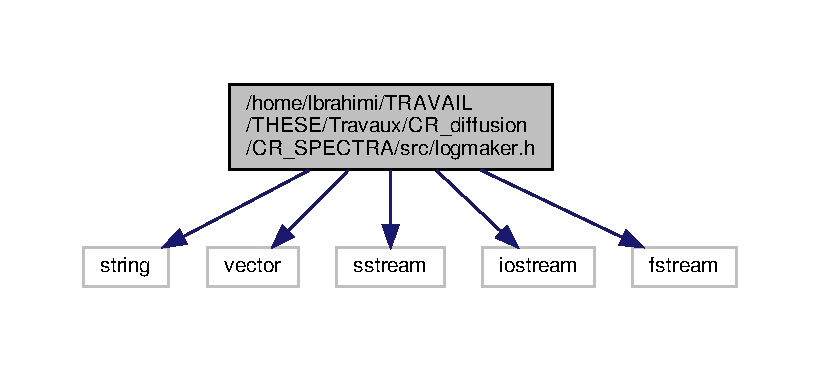
\includegraphics[width=350pt]{logmaker_8h__incl}
\end{center}
\end{figure}
This graph shows which files directly or indirectly include this file\+:\nopagebreak
\begin{figure}[H]
\begin{center}
\leavevmode
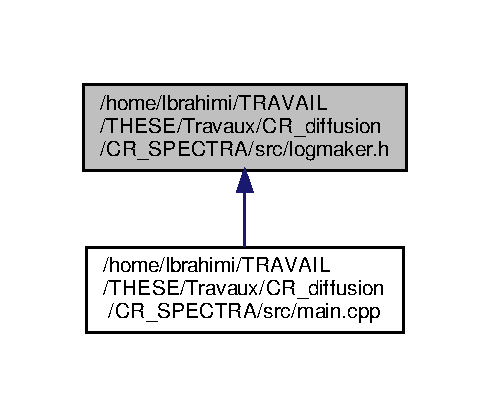
\includegraphics[width=235pt]{logmaker_8h__dep__incl}
\end{center}
\end{figure}
\subsection*{Functions}
\begin{DoxyCompactItemize}
\item 
void \hyperlink{logmaker_8h_a993d5f8f587684776ea27a5caf80ced9}{show\+Log\+\_\+0} (double time, double \hyperlink{constants_8h_a93e6f33b03669f059b9f0ec47810f624}{Tmax}, int nstep, int time\+\_\+id, double duration, double dt)
\end{DoxyCompactItemize}


\subsection{Function Documentation}
\mbox{\Hypertarget{logmaker_8h_a993d5f8f587684776ea27a5caf80ced9}\label{logmaker_8h_a993d5f8f587684776ea27a5caf80ced9}} 
\index{logmaker.\+h@{logmaker.\+h}!show\+Log\+\_\+0@{show\+Log\+\_\+0}}
\index{show\+Log\+\_\+0@{show\+Log\+\_\+0}!logmaker.\+h@{logmaker.\+h}}
\subsubsection{\texorpdfstring{show\+Log\+\_\+0()}{showLog\_0()}}
{\footnotesize\ttfamily void show\+Log\+\_\+0 (\begin{DoxyParamCaption}\item[{double}]{time,  }\item[{double}]{Tmax,  }\item[{int}]{nstep,  }\item[{int}]{time\+\_\+id,  }\item[{double}]{duration,  }\item[{double}]{dt }\end{DoxyParamCaption})}


\hypertarget{main_8cpp}{}\section{/home/lbrahimi/\+T\+R\+A\+V\+A\+I\+L/\+T\+H\+E\+S\+E/\+Travaux/\+C\+R\+\_\+diffusion/\+C\+R\+\_\+\+S\+P\+E\+C\+T\+R\+A/src/main.cpp File Reference}
\label{main_8cpp}\index{/home/lbrahimi/\+T\+R\+A\+V\+A\+I\+L/\+T\+H\+E\+S\+E/\+Travaux/\+C\+R\+\_\+diffusion/\+C\+R\+\_\+\+S\+P\+E\+C\+T\+R\+A/src/main.\+cpp@{/home/lbrahimi/\+T\+R\+A\+V\+A\+I\+L/\+T\+H\+E\+S\+E/\+Travaux/\+C\+R\+\_\+diffusion/\+C\+R\+\_\+\+S\+P\+E\+C\+T\+R\+A/src/main.\+cpp}}
{\ttfamily \#include $<$iostream$>$}\newline
{\ttfamily \#include $<$fstream$>$}\newline
{\ttfamily \#include $<$math.\+h$>$}\newline
{\ttfamily \#include $<$vector$>$}\newline
{\ttfamily \#include $<$string$>$}\newline
{\ttfamily \#include $<$tuple$>$}\newline
{\ttfamily \#include $<$cmath$>$}\newline
{\ttfamily \#include $<$sstream$>$}\newline
{\ttfamily \#include $<$ctime$>$}\newline
{\ttfamily \#include $<$chrono$>$}\newline
{\ttfamily \#include $<$thread$>$}\newline
{\ttfamily \#include $<$sys/resource.\+h$>$}\newline
{\ttfamily \#include $<$omp.\+h$>$}\newline
{\ttfamily \#include \char`\"{}./mathematics.\+h\char`\"{}}\newline
{\ttfamily \#include \char`\"{}./constants.\+h\char`\"{}}\newline
{\ttfamily \#include \char`\"{}./read2\+D.\+h\char`\"{}}\newline
{\ttfamily \#include \char`\"{}./freader.\+h\char`\"{}}\newline
{\ttfamily \#include \char`\"{}./fwritter.\+h\char`\"{}}\newline
{\ttfamily \#include \char`\"{}./out.\+h\char`\"{}}\newline
{\ttfamily \#include \char`\"{}./logmaker.\+h\char`\"{}}\newline
{\ttfamily \#include \char`\"{}./tools.\+h\char`\"{}}\newline
{\ttfamily \#include \char`\"{}./cr\+\_\+source.\+h\char`\"{}}\newline
{\ttfamily \#include \char`\"{}./solver1\+D.\+h\char`\"{}}\newline
Include dependency graph for main.\+cpp\+:\nopagebreak
\begin{figure}[H]
\begin{center}
\leavevmode
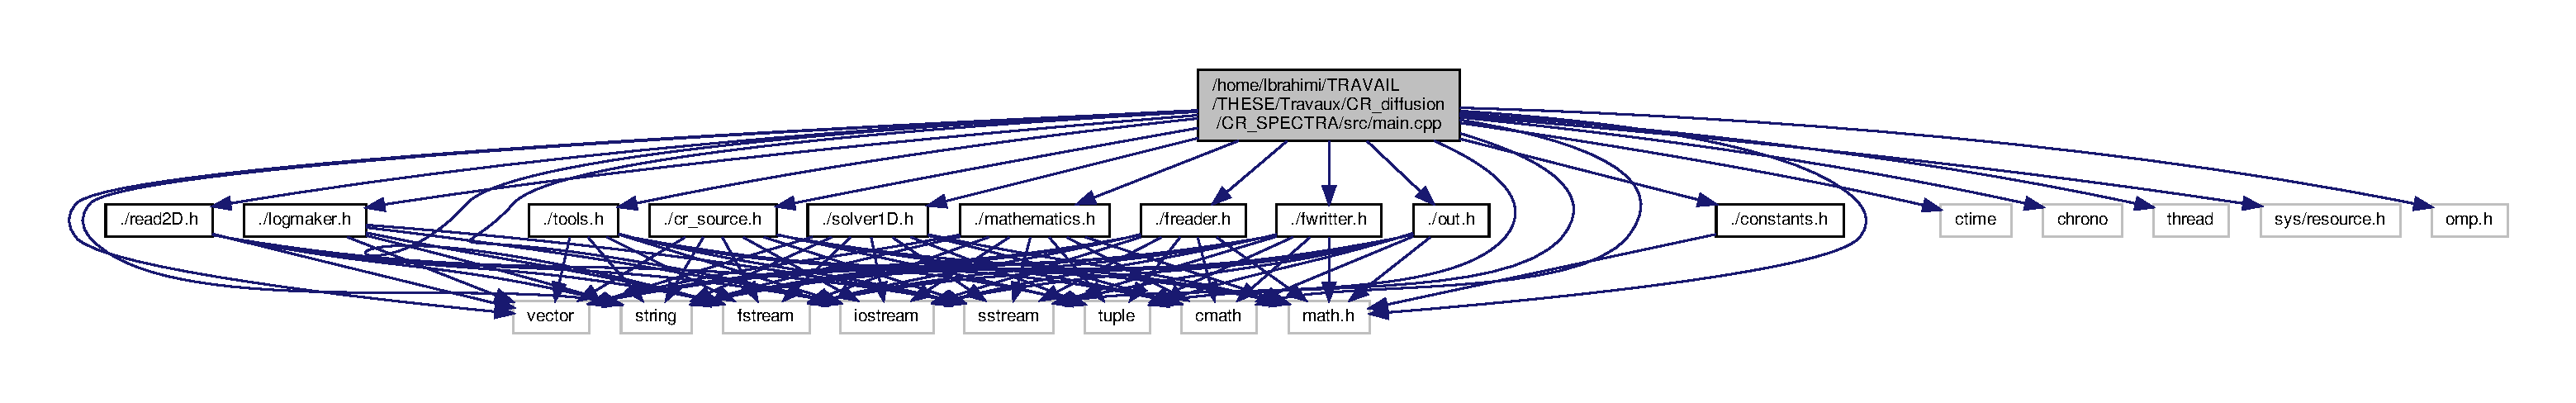
\includegraphics[width=350pt]{main_8cpp__incl}
\end{center}
\end{figure}
\subsection*{Functions}
\begin{DoxyCompactItemize}
\item 
int \hyperlink{main_8cpp_ae66f6b31b5ad750f1fe042a706a4e3d4}{main} ()
\end{DoxyCompactItemize}


\subsection{Function Documentation}
\mbox{\Hypertarget{main_8cpp_ae66f6b31b5ad750f1fe042a706a4e3d4}\label{main_8cpp_ae66f6b31b5ad750f1fe042a706a4e3d4}} 
\index{main.\+cpp@{main.\+cpp}!main@{main}}
\index{main@{main}!main.\+cpp@{main.\+cpp}}
\subsubsection{\texorpdfstring{main()}{main()}}
{\footnotesize\ttfamily int main (\begin{DoxyParamCaption}{ }\end{DoxyParamCaption})}


\hypertarget{mathematics_8h}{}\section{/home/lbrahimi/\+T\+R\+A\+V\+A\+I\+L/\+T\+H\+E\+S\+E/\+Travaux/\+C\+R\+\_\+diffusion/\+C\+R\+\_\+\+S\+P\+E\+C\+T\+R\+A/src/mathematics.h File Reference}
\label{mathematics_8h}\index{/home/lbrahimi/\+T\+R\+A\+V\+A\+I\+L/\+T\+H\+E\+S\+E/\+Travaux/\+C\+R\+\_\+diffusion/\+C\+R\+\_\+\+S\+P\+E\+C\+T\+R\+A/src/mathematics.\+h@{/home/lbrahimi/\+T\+R\+A\+V\+A\+I\+L/\+T\+H\+E\+S\+E/\+Travaux/\+C\+R\+\_\+diffusion/\+C\+R\+\_\+\+S\+P\+E\+C\+T\+R\+A/src/mathematics.\+h}}
{\ttfamily \#include $<$iostream$>$}\newline
{\ttfamily \#include $<$fstream$>$}\newline
{\ttfamily \#include $<$math.\+h$>$}\newline
{\ttfamily \#include $<$vector$>$}\newline
{\ttfamily \#include $<$string$>$}\newline
{\ttfamily \#include $<$tuple$>$}\newline
{\ttfamily \#include $<$cmath$>$}\newline
{\ttfamily \#include $<$sstream$>$}\newline
Include dependency graph for mathematics.\+h\+:\nopagebreak
\begin{figure}[H]
\begin{center}
\leavevmode
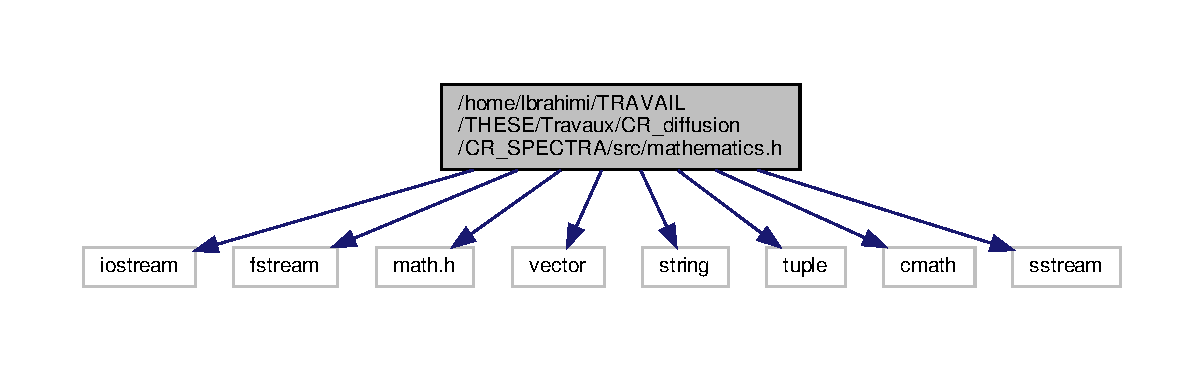
\includegraphics[width=350pt]{mathematics_8h__incl}
\end{center}
\end{figure}
This graph shows which files directly or indirectly include this file\+:\nopagebreak
\begin{figure}[H]
\begin{center}
\leavevmode
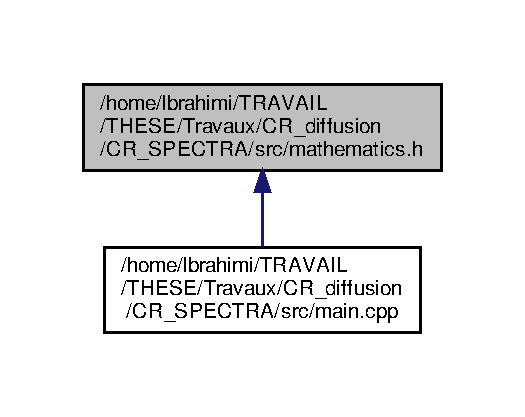
\includegraphics[width=252pt]{mathematics_8h__dep__incl}
\end{center}
\end{figure}
\subsection*{Functions}
\begin{DoxyCompactItemize}
\item 
vector$<$ double $>$ \hyperlink{mathematics_8h_a02b729c67d3c5a72bba364f4f7823e75}{T\+D\+MA} (vector$<$ double $>$ a, vector$<$ double $>$ b, vector$<$ double $>$ \hyperlink{constants_8h_a8fc6defe4e499b1b9b9c275689e44352}{c}, vector$<$ double $>$ d)
\item 
void \hyperlink{mathematics_8h_af44c170fbc162ede50cb386365a8d48a}{Inverse\+Trigonal\+Matrix} (vector$<$ vector$<$ double $>$ $>$ \&\hyperlink{cr__source_8h_ac94a6e5794c2d7b59588b14025cfba20}{T})
\item 
void \hyperlink{mathematics_8h_a845310c9a1bf4e842d8a38d8b8375965}{Product\+Matrix} (vector$<$ vector$<$ double $>$ $>$ A, vector$<$ vector$<$ double $>$ $>$ B, vector$<$ vector$<$ double $>$ $>$ \&C)
\item 
double \hyperlink{mathematics_8h_aa9efdc9b8bb19a51263aef089b14a129}{Interpolating\+Spline} (vector$<$ double $>$ X, vector$<$ double $>$ Y, double x)
\item 
double \hyperlink{mathematics_8h_a805401e62bc01cb980c2d557a49df39e}{f1} (double x, vector$<$ double $>$ cst)
\item 
double \hyperlink{mathematics_8h_ac46d60428d36cd0411aab53e0f8c62f1}{df1dx} (double x, vector$<$ double $>$ cst)
\item 
double \hyperlink{mathematics_8h_adf6736ed28f61682cb8f2df704ab5931}{f2} (double x, vector$<$ double $>$ cst)
\item 
double \hyperlink{mathematics_8h_a4c0a27106143a8b884cf1fa28b143c7f}{df2dx} (double x, vector$<$ double $>$ cst)
\item 
double \hyperlink{mathematics_8h_a4f8505bc6e6ab1f8925b57cb302ef8f4}{Newton\+Raphson} (double f(double, vector$<$ double $>$), double df(double, vector$<$ double $>$), double x0, double eps, vector$<$ double $>$ cst)
\item 
double \hyperlink{mathematics_8h_a7baa564a665524bae08b142f23a4ebf7}{Get\+Max} (vector$<$ double $>$ V)
\item 
void \hyperlink{mathematics_8h_a0627a885cb985510408fa0728190aca7}{transpose} (vector$<$ vector$<$ double $>$ $>$ \&b, vector$<$ vector$<$ double $>$ $>$ \&\hyperlink{constants_8h_a8fc6defe4e499b1b9b9c275689e44352}{c})
\item 
double \hyperlink{mathematics_8h_afe33a99d5b0c642b27c9abff1a16f0d0}{minmod} (double a, double b)
\end{DoxyCompactItemize}


\subsection{Function Documentation}
\mbox{\Hypertarget{mathematics_8h_ac46d60428d36cd0411aab53e0f8c62f1}\label{mathematics_8h_ac46d60428d36cd0411aab53e0f8c62f1}} 
\index{mathematics.\+h@{mathematics.\+h}!df1dx@{df1dx}}
\index{df1dx@{df1dx}!mathematics.\+h@{mathematics.\+h}}
\subsubsection{\texorpdfstring{df1dx()}{df1dx()}}
{\footnotesize\ttfamily double df1dx (\begin{DoxyParamCaption}\item[{double}]{x,  }\item[{vector$<$ double $>$}]{cst }\end{DoxyParamCaption})}

\mbox{\Hypertarget{mathematics_8h_a4c0a27106143a8b884cf1fa28b143c7f}\label{mathematics_8h_a4c0a27106143a8b884cf1fa28b143c7f}} 
\index{mathematics.\+h@{mathematics.\+h}!df2dx@{df2dx}}
\index{df2dx@{df2dx}!mathematics.\+h@{mathematics.\+h}}
\subsubsection{\texorpdfstring{df2dx()}{df2dx()}}
{\footnotesize\ttfamily double df2dx (\begin{DoxyParamCaption}\item[{double}]{x,  }\item[{vector$<$ double $>$}]{cst }\end{DoxyParamCaption})}

\mbox{\Hypertarget{mathematics_8h_a805401e62bc01cb980c2d557a49df39e}\label{mathematics_8h_a805401e62bc01cb980c2d557a49df39e}} 
\index{mathematics.\+h@{mathematics.\+h}!f1@{f1}}
\index{f1@{f1}!mathematics.\+h@{mathematics.\+h}}
\subsubsection{\texorpdfstring{f1()}{f1()}}
{\footnotesize\ttfamily double f1 (\begin{DoxyParamCaption}\item[{double}]{x,  }\item[{vector$<$ double $>$}]{cst }\end{DoxyParamCaption})}

\mbox{\Hypertarget{mathematics_8h_adf6736ed28f61682cb8f2df704ab5931}\label{mathematics_8h_adf6736ed28f61682cb8f2df704ab5931}} 
\index{mathematics.\+h@{mathematics.\+h}!f2@{f2}}
\index{f2@{f2}!mathematics.\+h@{mathematics.\+h}}
\subsubsection{\texorpdfstring{f2()}{f2()}}
{\footnotesize\ttfamily double f2 (\begin{DoxyParamCaption}\item[{double}]{x,  }\item[{vector$<$ double $>$}]{cst }\end{DoxyParamCaption})}

\mbox{\Hypertarget{mathematics_8h_a7baa564a665524bae08b142f23a4ebf7}\label{mathematics_8h_a7baa564a665524bae08b142f23a4ebf7}} 
\index{mathematics.\+h@{mathematics.\+h}!Get\+Max@{Get\+Max}}
\index{Get\+Max@{Get\+Max}!mathematics.\+h@{mathematics.\+h}}
\subsubsection{\texorpdfstring{Get\+Max()}{GetMax()}}
{\footnotesize\ttfamily double Get\+Max (\begin{DoxyParamCaption}\item[{vector$<$ double $>$}]{V }\end{DoxyParamCaption})}

\mbox{\Hypertarget{mathematics_8h_aa9efdc9b8bb19a51263aef089b14a129}\label{mathematics_8h_aa9efdc9b8bb19a51263aef089b14a129}} 
\index{mathematics.\+h@{mathematics.\+h}!Interpolating\+Spline@{Interpolating\+Spline}}
\index{Interpolating\+Spline@{Interpolating\+Spline}!mathematics.\+h@{mathematics.\+h}}
\subsubsection{\texorpdfstring{Interpolating\+Spline()}{InterpolatingSpline()}}
{\footnotesize\ttfamily double Interpolating\+Spline (\begin{DoxyParamCaption}\item[{vector$<$ double $>$}]{X,  }\item[{vector$<$ double $>$}]{Y,  }\item[{double}]{x }\end{DoxyParamCaption})}

\mbox{\Hypertarget{mathematics_8h_af44c170fbc162ede50cb386365a8d48a}\label{mathematics_8h_af44c170fbc162ede50cb386365a8d48a}} 
\index{mathematics.\+h@{mathematics.\+h}!Inverse\+Trigonal\+Matrix@{Inverse\+Trigonal\+Matrix}}
\index{Inverse\+Trigonal\+Matrix@{Inverse\+Trigonal\+Matrix}!mathematics.\+h@{mathematics.\+h}}
\subsubsection{\texorpdfstring{Inverse\+Trigonal\+Matrix()}{InverseTrigonalMatrix()}}
{\footnotesize\ttfamily void Inverse\+Trigonal\+Matrix (\begin{DoxyParamCaption}\item[{vector$<$ vector$<$ double $>$ $>$ \&}]{T }\end{DoxyParamCaption})}

\mbox{\Hypertarget{mathematics_8h_afe33a99d5b0c642b27c9abff1a16f0d0}\label{mathematics_8h_afe33a99d5b0c642b27c9abff1a16f0d0}} 
\index{mathematics.\+h@{mathematics.\+h}!minmod@{minmod}}
\index{minmod@{minmod}!mathematics.\+h@{mathematics.\+h}}
\subsubsection{\texorpdfstring{minmod()}{minmod()}}
{\footnotesize\ttfamily double minmod (\begin{DoxyParamCaption}\item[{double}]{a,  }\item[{double}]{b }\end{DoxyParamCaption})}

\mbox{\Hypertarget{mathematics_8h_a4f8505bc6e6ab1f8925b57cb302ef8f4}\label{mathematics_8h_a4f8505bc6e6ab1f8925b57cb302ef8f4}} 
\index{mathematics.\+h@{mathematics.\+h}!Newton\+Raphson@{Newton\+Raphson}}
\index{Newton\+Raphson@{Newton\+Raphson}!mathematics.\+h@{mathematics.\+h}}
\subsubsection{\texorpdfstring{Newton\+Raphson()}{NewtonRaphson()}}
{\footnotesize\ttfamily double Newton\+Raphson (\begin{DoxyParamCaption}\item[{double }]{fdouble, vector$<$ double $>$,  }\item[{double }]{dfdouble, vector$<$ double $>$,  }\item[{double}]{x0,  }\item[{double}]{eps,  }\item[{vector$<$ double $>$}]{cst }\end{DoxyParamCaption})}

\mbox{\Hypertarget{mathematics_8h_a845310c9a1bf4e842d8a38d8b8375965}\label{mathematics_8h_a845310c9a1bf4e842d8a38d8b8375965}} 
\index{mathematics.\+h@{mathematics.\+h}!Product\+Matrix@{Product\+Matrix}}
\index{Product\+Matrix@{Product\+Matrix}!mathematics.\+h@{mathematics.\+h}}
\subsubsection{\texorpdfstring{Product\+Matrix()}{ProductMatrix()}}
{\footnotesize\ttfamily void Product\+Matrix (\begin{DoxyParamCaption}\item[{vector$<$ vector$<$ double $>$ $>$}]{A,  }\item[{vector$<$ vector$<$ double $>$ $>$}]{B,  }\item[{vector$<$ vector$<$ double $>$ $>$ \&}]{C }\end{DoxyParamCaption})}

\mbox{\Hypertarget{mathematics_8h_a02b729c67d3c5a72bba364f4f7823e75}\label{mathematics_8h_a02b729c67d3c5a72bba364f4f7823e75}} 
\index{mathematics.\+h@{mathematics.\+h}!T\+D\+MA@{T\+D\+MA}}
\index{T\+D\+MA@{T\+D\+MA}!mathematics.\+h@{mathematics.\+h}}
\subsubsection{\texorpdfstring{T\+D\+M\+A()}{TDMA()}}
{\footnotesize\ttfamily vector$<$double$>$ T\+D\+MA (\begin{DoxyParamCaption}\item[{vector$<$ double $>$}]{a,  }\item[{vector$<$ double $>$}]{b,  }\item[{vector$<$ double $>$}]{c,  }\item[{vector$<$ double $>$}]{d }\end{DoxyParamCaption})}

\mbox{\Hypertarget{mathematics_8h_a0627a885cb985510408fa0728190aca7}\label{mathematics_8h_a0627a885cb985510408fa0728190aca7}} 
\index{mathematics.\+h@{mathematics.\+h}!transpose@{transpose}}
\index{transpose@{transpose}!mathematics.\+h@{mathematics.\+h}}
\subsubsection{\texorpdfstring{transpose()}{transpose()}}
{\footnotesize\ttfamily void transpose (\begin{DoxyParamCaption}\item[{vector$<$ vector$<$ double $>$ $>$ \&}]{b,  }\item[{vector$<$ vector$<$ double $>$ $>$ \&}]{c }\end{DoxyParamCaption})}


\hypertarget{cr__escape_8cpp}{}\section{/home/lbrahimi/\+T\+R\+A\+V\+A\+I\+L/\+T\+H\+E\+S\+E/\+Travaux/\+C\+R\+\_\+diffusion/\+C\+R\+\_\+\+S\+P\+E\+C\+T\+R\+A/src/others/cr\+\_\+escape.cpp File Reference}
\label{cr__escape_8cpp}\index{/home/lbrahimi/\+T\+R\+A\+V\+A\+I\+L/\+T\+H\+E\+S\+E/\+Travaux/\+C\+R\+\_\+diffusion/\+C\+R\+\_\+\+S\+P\+E\+C\+T\+R\+A/src/others/cr\+\_\+escape.\+cpp@{/home/lbrahimi/\+T\+R\+A\+V\+A\+I\+L/\+T\+H\+E\+S\+E/\+Travaux/\+C\+R\+\_\+diffusion/\+C\+R\+\_\+\+S\+P\+E\+C\+T\+R\+A/src/others/cr\+\_\+escape.\+cpp}}
{\ttfamily \#include $<$iostream$>$}\newline
{\ttfamily \#include $<$fstream$>$}\newline
{\ttfamily \#include $<$math.\+h$>$}\newline
{\ttfamily \#include $<$vector$>$}\newline
{\ttfamily \#include $<$string$>$}\newline
{\ttfamily \#include $<$tuple$>$}\newline
{\ttfamily \#include $<$cmath$>$}\newline
{\ttfamily \#include $<$sstream$>$}\newline
Include dependency graph for cr\+\_\+escape.\+cpp\+:\nopagebreak
\begin{figure}[H]
\begin{center}
\leavevmode
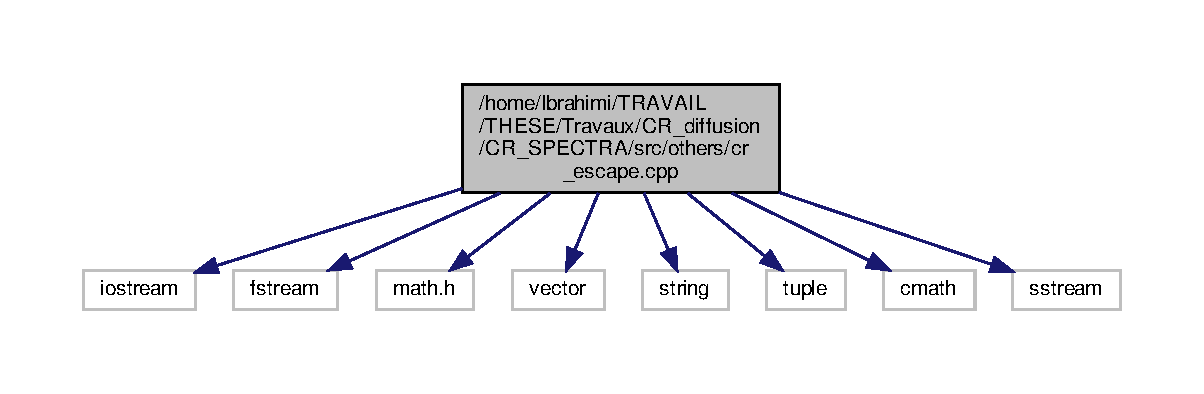
\includegraphics[width=350pt]{cr__escape_8cpp__incl}
\end{center}
\end{figure}
\subsection*{Functions}
\begin{DoxyCompactItemize}
\item 
void \hyperlink{cr__escape_8cpp_af44c170fbc162ede50cb386365a8d48a}{Inverse\+Trigonal\+Matrix} (vector$<$ vector$<$ double $>$ $>$ \&\hyperlink{cr__source_8h_ac94a6e5794c2d7b59588b14025cfba20}{T})
\item 
void \hyperlink{cr__escape_8cpp_a845310c9a1bf4e842d8a38d8b8375965}{Product\+Matrix} (vector$<$ vector$<$ double $>$ $>$ A, vector$<$ vector$<$ double $>$ $>$ B, vector$<$ vector$<$ double $>$ $>$ \&C)
\item 
double \hyperlink{cr__escape_8cpp_aa9efdc9b8bb19a51263aef089b14a129}{Interpolating\+Spline} (vector$<$ double $>$ X, vector$<$ double $>$ Y, double x)
\item 
double \hyperlink{cr__escape_8cpp_a805401e62bc01cb980c2d557a49df39e}{f1} (double x, vector$<$ double $>$ cst)
\item 
double \hyperlink{cr__escape_8cpp_ac46d60428d36cd0411aab53e0f8c62f1}{df1dx} (double x, vector$<$ double $>$ cst)
\item 
double \hyperlink{cr__escape_8cpp_adf6736ed28f61682cb8f2df704ab5931}{f2} (double x, vector$<$ double $>$ cst)
\item 
double \hyperlink{cr__escape_8cpp_a4c0a27106143a8b884cf1fa28b143c7f}{df2dx} (double x, vector$<$ double $>$ cst)
\item 
double \hyperlink{cr__escape_8cpp_a4f8505bc6e6ab1f8925b57cb302ef8f4}{Newton\+Raphson} (double f(double, vector$<$ double $>$), double df(double, vector$<$ double $>$), double x0, double eps, vector$<$ double $>$ cst)
\item 
double \hyperlink{cr__escape_8cpp_a7baa564a665524bae08b142f23a4ebf7}{Get\+Max} (vector$<$ double $>$ V)
\item 
double \hyperlink{cr__escape_8cpp_aacef4afde13abf90336dd75fb4cbf7a0}{Get\+Tesc} (double E, double \hyperlink{constants_8h_a80a3c65c6b77216165fc34c12d0744e9}{delta}, vector$<$ double $>$ cst)
\item 
int \hyperlink{cr__escape_8cpp_ae66f6b31b5ad750f1fe042a706a4e3d4}{main} ()
\end{DoxyCompactItemize}


\subsection{Function Documentation}
\mbox{\Hypertarget{cr__escape_8cpp_ac46d60428d36cd0411aab53e0f8c62f1}\label{cr__escape_8cpp_ac46d60428d36cd0411aab53e0f8c62f1}} 
\index{cr\+\_\+escape.\+cpp@{cr\+\_\+escape.\+cpp}!df1dx@{df1dx}}
\index{df1dx@{df1dx}!cr\+\_\+escape.\+cpp@{cr\+\_\+escape.\+cpp}}
\subsubsection{\texorpdfstring{df1dx()}{df1dx()}}
{\footnotesize\ttfamily double df1dx (\begin{DoxyParamCaption}\item[{double}]{x,  }\item[{vector$<$ double $>$}]{cst }\end{DoxyParamCaption})}

\mbox{\Hypertarget{cr__escape_8cpp_a4c0a27106143a8b884cf1fa28b143c7f}\label{cr__escape_8cpp_a4c0a27106143a8b884cf1fa28b143c7f}} 
\index{cr\+\_\+escape.\+cpp@{cr\+\_\+escape.\+cpp}!df2dx@{df2dx}}
\index{df2dx@{df2dx}!cr\+\_\+escape.\+cpp@{cr\+\_\+escape.\+cpp}}
\subsubsection{\texorpdfstring{df2dx()}{df2dx()}}
{\footnotesize\ttfamily double df2dx (\begin{DoxyParamCaption}\item[{double}]{x,  }\item[{vector$<$ double $>$}]{cst }\end{DoxyParamCaption})}

\mbox{\Hypertarget{cr__escape_8cpp_a805401e62bc01cb980c2d557a49df39e}\label{cr__escape_8cpp_a805401e62bc01cb980c2d557a49df39e}} 
\index{cr\+\_\+escape.\+cpp@{cr\+\_\+escape.\+cpp}!f1@{f1}}
\index{f1@{f1}!cr\+\_\+escape.\+cpp@{cr\+\_\+escape.\+cpp}}
\subsubsection{\texorpdfstring{f1()}{f1()}}
{\footnotesize\ttfamily double f1 (\begin{DoxyParamCaption}\item[{double}]{x,  }\item[{vector$<$ double $>$}]{cst }\end{DoxyParamCaption})}

\mbox{\Hypertarget{cr__escape_8cpp_adf6736ed28f61682cb8f2df704ab5931}\label{cr__escape_8cpp_adf6736ed28f61682cb8f2df704ab5931}} 
\index{cr\+\_\+escape.\+cpp@{cr\+\_\+escape.\+cpp}!f2@{f2}}
\index{f2@{f2}!cr\+\_\+escape.\+cpp@{cr\+\_\+escape.\+cpp}}
\subsubsection{\texorpdfstring{f2()}{f2()}}
{\footnotesize\ttfamily double f2 (\begin{DoxyParamCaption}\item[{double}]{x,  }\item[{vector$<$ double $>$}]{cst }\end{DoxyParamCaption})}

\mbox{\Hypertarget{cr__escape_8cpp_a7baa564a665524bae08b142f23a4ebf7}\label{cr__escape_8cpp_a7baa564a665524bae08b142f23a4ebf7}} 
\index{cr\+\_\+escape.\+cpp@{cr\+\_\+escape.\+cpp}!Get\+Max@{Get\+Max}}
\index{Get\+Max@{Get\+Max}!cr\+\_\+escape.\+cpp@{cr\+\_\+escape.\+cpp}}
\subsubsection{\texorpdfstring{Get\+Max()}{GetMax()}}
{\footnotesize\ttfamily double Get\+Max (\begin{DoxyParamCaption}\item[{vector$<$ double $>$}]{V }\end{DoxyParamCaption})}

\mbox{\Hypertarget{cr__escape_8cpp_aacef4afde13abf90336dd75fb4cbf7a0}\label{cr__escape_8cpp_aacef4afde13abf90336dd75fb4cbf7a0}} 
\index{cr\+\_\+escape.\+cpp@{cr\+\_\+escape.\+cpp}!Get\+Tesc@{Get\+Tesc}}
\index{Get\+Tesc@{Get\+Tesc}!cr\+\_\+escape.\+cpp@{cr\+\_\+escape.\+cpp}}
\subsubsection{\texorpdfstring{Get\+Tesc()}{GetTesc()}}
{\footnotesize\ttfamily double Get\+Tesc (\begin{DoxyParamCaption}\item[{double}]{E,  }\item[{double}]{delta,  }\item[{vector$<$ double $>$}]{cst }\end{DoxyParamCaption})}

\mbox{\Hypertarget{cr__escape_8cpp_aa9efdc9b8bb19a51263aef089b14a129}\label{cr__escape_8cpp_aa9efdc9b8bb19a51263aef089b14a129}} 
\index{cr\+\_\+escape.\+cpp@{cr\+\_\+escape.\+cpp}!Interpolating\+Spline@{Interpolating\+Spline}}
\index{Interpolating\+Spline@{Interpolating\+Spline}!cr\+\_\+escape.\+cpp@{cr\+\_\+escape.\+cpp}}
\subsubsection{\texorpdfstring{Interpolating\+Spline()}{InterpolatingSpline()}}
{\footnotesize\ttfamily double Interpolating\+Spline (\begin{DoxyParamCaption}\item[{vector$<$ double $>$}]{X,  }\item[{vector$<$ double $>$}]{Y,  }\item[{double}]{x }\end{DoxyParamCaption})}

\mbox{\Hypertarget{cr__escape_8cpp_af44c170fbc162ede50cb386365a8d48a}\label{cr__escape_8cpp_af44c170fbc162ede50cb386365a8d48a}} 
\index{cr\+\_\+escape.\+cpp@{cr\+\_\+escape.\+cpp}!Inverse\+Trigonal\+Matrix@{Inverse\+Trigonal\+Matrix}}
\index{Inverse\+Trigonal\+Matrix@{Inverse\+Trigonal\+Matrix}!cr\+\_\+escape.\+cpp@{cr\+\_\+escape.\+cpp}}
\subsubsection{\texorpdfstring{Inverse\+Trigonal\+Matrix()}{InverseTrigonalMatrix()}}
{\footnotesize\ttfamily void Inverse\+Trigonal\+Matrix (\begin{DoxyParamCaption}\item[{vector$<$ vector$<$ double $>$ $>$ \&}]{T }\end{DoxyParamCaption})}

\mbox{\Hypertarget{cr__escape_8cpp_ae66f6b31b5ad750f1fe042a706a4e3d4}\label{cr__escape_8cpp_ae66f6b31b5ad750f1fe042a706a4e3d4}} 
\index{cr\+\_\+escape.\+cpp@{cr\+\_\+escape.\+cpp}!main@{main}}
\index{main@{main}!cr\+\_\+escape.\+cpp@{cr\+\_\+escape.\+cpp}}
\subsubsection{\texorpdfstring{main()}{main()}}
{\footnotesize\ttfamily int main (\begin{DoxyParamCaption}{ }\end{DoxyParamCaption})}

\mbox{\Hypertarget{cr__escape_8cpp_a4f8505bc6e6ab1f8925b57cb302ef8f4}\label{cr__escape_8cpp_a4f8505bc6e6ab1f8925b57cb302ef8f4}} 
\index{cr\+\_\+escape.\+cpp@{cr\+\_\+escape.\+cpp}!Newton\+Raphson@{Newton\+Raphson}}
\index{Newton\+Raphson@{Newton\+Raphson}!cr\+\_\+escape.\+cpp@{cr\+\_\+escape.\+cpp}}
\subsubsection{\texorpdfstring{Newton\+Raphson()}{NewtonRaphson()}}
{\footnotesize\ttfamily double Newton\+Raphson (\begin{DoxyParamCaption}\item[{double }]{fdouble, vector$<$ double $>$,  }\item[{double }]{dfdouble, vector$<$ double $>$,  }\item[{double}]{x0,  }\item[{double}]{eps,  }\item[{vector$<$ double $>$}]{cst }\end{DoxyParamCaption})}

\mbox{\Hypertarget{cr__escape_8cpp_a845310c9a1bf4e842d8a38d8b8375965}\label{cr__escape_8cpp_a845310c9a1bf4e842d8a38d8b8375965}} 
\index{cr\+\_\+escape.\+cpp@{cr\+\_\+escape.\+cpp}!Product\+Matrix@{Product\+Matrix}}
\index{Product\+Matrix@{Product\+Matrix}!cr\+\_\+escape.\+cpp@{cr\+\_\+escape.\+cpp}}
\subsubsection{\texorpdfstring{Product\+Matrix()}{ProductMatrix()}}
{\footnotesize\ttfamily void Product\+Matrix (\begin{DoxyParamCaption}\item[{vector$<$ vector$<$ double $>$ $>$}]{A,  }\item[{vector$<$ vector$<$ double $>$ $>$}]{B,  }\item[{vector$<$ vector$<$ double $>$ $>$ \&}]{C }\end{DoxyParamCaption})}


\hypertarget{PDE__solvers_8py}{}\section{/home/lbrahimi/\+T\+R\+A\+V\+A\+I\+L/\+T\+H\+E\+S\+E/\+Travaux/\+C\+R\+\_\+diffusion/\+C\+R\+\_\+\+S\+P\+E\+C\+T\+R\+A/src/others/\+P\+D\+E\+\_\+solvers.py File Reference}
\label{PDE__solvers_8py}\index{/home/lbrahimi/\+T\+R\+A\+V\+A\+I\+L/\+T\+H\+E\+S\+E/\+Travaux/\+C\+R\+\_\+diffusion/\+C\+R\+\_\+\+S\+P\+E\+C\+T\+R\+A/src/others/\+P\+D\+E\+\_\+solvers.\+py@{/home/lbrahimi/\+T\+R\+A\+V\+A\+I\+L/\+T\+H\+E\+S\+E/\+Travaux/\+C\+R\+\_\+diffusion/\+C\+R\+\_\+\+S\+P\+E\+C\+T\+R\+A/src/others/\+P\+D\+E\+\_\+solvers.\+py}}
\subsection*{Namespaces}
\begin{DoxyCompactItemize}
\item 
 \hyperlink{namespacePDE__solvers}{P\+D\+E\+\_\+solvers}
\end{DoxyCompactItemize}
\subsection*{Functions}
\begin{DoxyCompactItemize}
\item 
def \hyperlink{namespacePDE__solvers_a7e8f1dede17ef38bf75b8db7cee5bf38}{P\+D\+E\+\_\+solvers.\+T\+D\+MA} (a, b, \hyperlink{constants_8h_a8fc6defe4e499b1b9b9c275689e44352}{c}, d)
\item 
def \hyperlink{namespacePDE__solvers_a01e04051a07f5e380f02fa1a2a000531}{P\+D\+E\+\_\+solvers.\+A} (x)
\item 
def \hyperlink{namespacePDE__solvers_a209625175ace8add9160ffa5438c150a}{P\+D\+E\+\_\+solvers.\+B} (x)
\item 
def \hyperlink{namespacePDE__solvers_a2f40c0a059e412453818e6482fb92b09}{P\+D\+E\+\_\+solvers.\+C} (x)
\item 
def \hyperlink{namespacePDE__solvers_a4e422ca6c34b0d9d943190ee570abb08}{P\+D\+E\+\_\+solvers.\+Q} (x)
\item 
def \hyperlink{namespacePDE__solvers_a6728696b430071890e97671c2c6069fa}{P\+D\+E\+\_\+solvers.\+T} (x)
\item 
def \hyperlink{namespacePDE__solvers_a306ac1abd1ee9ac53a496bbb64eac157}{P\+D\+E\+\_\+solvers.\+finite\+Diff\+Solver} (dt, \hyperlink{constants_8h_a93e6f33b03669f059b9f0ec47810f624}{Tmax}, u)
\item 
def \hyperlink{namespacePDE__solvers_a093eb37c7beab9cbd84f388e77821fce}{P\+D\+E\+\_\+solvers.\+Simple\+Implicit\+Solver} (dt, \hyperlink{constants_8h_a93e6f33b03669f059b9f0ec47810f624}{Tmax}, u)
\item 
def \hyperlink{namespacePDE__solvers_aeb1cc15f3da8633c104496a7cb7aa83c}{P\+D\+E\+\_\+solvers.\+C\+C70\+Solver} (dt, \hyperlink{constants_8h_a93e6f33b03669f059b9f0ec47810f624}{Tmax}, u)
\end{DoxyCompactItemize}
\subsection*{Variables}
\begin{DoxyCompactItemize}
\item 
float \hyperlink{namespacePDE__solvers_a71c07d7118cdda8c71573599545d0017}{P\+D\+E\+\_\+solvers.\+pc} = 3.\+086e18
\begin{DoxyCompactList}\small\item\em Tri Diagonal Matrix Algorithm(a.\+k.\+a Thomas algorithm) solver def T\+D\+M\+Asolver(a, b, c, d)\+: \textquotesingle{}\textquotesingle{}\textquotesingle{} T\+D\+MA solver, a b c d can be Num\+Py array type or Python list type. \end{DoxyCompactList}\item 
float \hyperlink{namespacePDE__solvers_a400304049742ae9f9b048c40cb6a52cb}{P\+D\+E\+\_\+solvers.\+yr} = 365.\+25$\ast$86400
\item 
int \hyperlink{namespacePDE__solvers_a17e611d575d9a8bda46ea6b596138f12}{P\+D\+E\+\_\+solvers.\+kyr} = 1e3$\ast$yr
\item 
int \hyperlink{namespacePDE__solvers_a9d6fca7c2abdff4c2c7feec55d437940}{P\+D\+E\+\_\+solvers.\+M} = 2048
\item 
int \hyperlink{namespacePDE__solvers_a7a1ac835675841b757a70f18b51246dc}{P\+D\+E\+\_\+solvers.\+Xmin} = 0.
\item 
int \hyperlink{namespacePDE__solvers_a48fb209db97ce5937802d0a747fb9991}{P\+D\+E\+\_\+solvers.\+Xmax} = 1000.$\ast$\hyperlink{constants_8h_a2884cd030c4c825754349a525a1d06ce}{pc}
\item 
\hyperlink{namespacePDE__solvers_ab53183fc05bd900f7013cd056e2e7338}{P\+D\+E\+\_\+solvers.\+X} = np.\+linspace(Xmin, Xmax, M+1)
\item 
\hyperlink{namespacePDE__solvers_abaa9fdf113a88661fc0afa93032755d3}{P\+D\+E\+\_\+solvers.\+u} = np.\+zeros(M+1)
\begin{DoxyCompactList}\small\item\em plt.\+semilogy(X/pc, u, c=\char`\"{}blue\char`\"{}) plt.\+plot(X/pc, u/U, c=\char`\"{}red\char`\"{}) plt.\+axhline(1.) print (\char`\"{}ratio = \char`\"{},sum(u)/sum(U)) \end{DoxyCompactList}\item 
\hyperlink{namespacePDE__solvers_aecb3894d7f844fe950ec6e4eb6ab14c6}{P\+D\+E\+\_\+solvers.\+u0} = u\mbox{[}1\mbox{]}
\item 
\hyperlink{namespacePDE__solvers_acd452357e85c033220a4da5bc3f71966}{P\+D\+E\+\_\+solvers.\+uM} = u\mbox{[}M-\/1\mbox{]}
\item 
\hyperlink{namespacePDE__solvers_a2184f2624ab571a00cfedb3a2a45cfaf}{P\+D\+E\+\_\+solvers.\+u\+\_\+ini} = u.\+copy()
\item 
\hyperlink{namespacePDE__solvers_afddf2b29ad67e3711d02129f93615761}{P\+D\+E\+\_\+solvers.\+u\+\_\+end} = u
\item 
int \hyperlink{namespacePDE__solvers_acdfd09d09c00385a3f3574d55d7e54a9}{P\+D\+E\+\_\+solvers.\+Tmax} = 10.$\ast$\hyperlink{constants_8h_a0edf155739e92555799f4a04b10af6bf}{kyr}
\item 
def \hyperlink{namespacePDE__solvers_a841654a1a841e1aca6f253e271b158c8}{P\+D\+E\+\_\+solvers.\+u\+\_\+0} = C\+C70\+Solver(0.\+1$\ast$\hyperlink{constants_8h_a0edf155739e92555799f4a04b10af6bf}{kyr}, \hyperlink{constants_8h_a93e6f33b03669f059b9f0ec47810f624}{Tmax}, u)
\item 
def \hyperlink{namespacePDE__solvers_a16bfb4d8d2eb6d1a005652edf340bc53}{P\+D\+E\+\_\+solvers.\+u\+\_\+1} = C\+C70\+Solver(0.\+5$\ast$\hyperlink{constants_8h_a0edf155739e92555799f4a04b10af6bf}{kyr}, \hyperlink{constants_8h_a93e6f33b03669f059b9f0ec47810f624}{Tmax}, u)
\item 
def \hyperlink{namespacePDE__solvers_a37d193fe9e294403c8a7145a75caacb3}{P\+D\+E\+\_\+solvers.\+u\+\_\+2} = C\+C70\+Solver(5.$\ast$\hyperlink{constants_8h_a0edf155739e92555799f4a04b10af6bf}{kyr}, \hyperlink{constants_8h_a93e6f33b03669f059b9f0ec47810f624}{Tmax}, u)
\item 
\hyperlink{namespacePDE__solvers_a129441ff5bc2a944435b54ac29fa70df}{P\+D\+E\+\_\+solvers.\+figsize}
\item 
\hyperlink{namespacePDE__solvers_a730023a0d9af5165d835a6dcc10e67d2}{P\+D\+E\+\_\+solvers.\+c}
\end{DoxyCompactItemize}

\hypertarget{Split__solvers_8py}{}\section{/home/lbrahimi/\+T\+R\+A\+V\+A\+I\+L/\+T\+H\+E\+S\+E/\+Travaux/\+C\+R\+\_\+diffusion/\+C\+R\+\_\+\+S\+P\+E\+C\+T\+R\+A/src/others/\+Split\+\_\+solvers.py File Reference}
\label{Split__solvers_8py}\index{/home/lbrahimi/\+T\+R\+A\+V\+A\+I\+L/\+T\+H\+E\+S\+E/\+Travaux/\+C\+R\+\_\+diffusion/\+C\+R\+\_\+\+S\+P\+E\+C\+T\+R\+A/src/others/\+Split\+\_\+solvers.\+py@{/home/lbrahimi/\+T\+R\+A\+V\+A\+I\+L/\+T\+H\+E\+S\+E/\+Travaux/\+C\+R\+\_\+diffusion/\+C\+R\+\_\+\+S\+P\+E\+C\+T\+R\+A/src/others/\+Split\+\_\+solvers.\+py}}
\subsection*{Namespaces}
\begin{DoxyCompactItemize}
\item 
 \hyperlink{namespaceSplit__solvers}{Split\+\_\+solvers}
\end{DoxyCompactItemize}
\subsection*{Functions}
\begin{DoxyCompactItemize}
\item 
def \hyperlink{namespaceSplit__solvers_afbe15271a0fe5821bdfe8760325cb4bb}{Split\+\_\+solvers.\+T\+D\+MA} (a, b, \hyperlink{constants_8h_a8fc6defe4e499b1b9b9c275689e44352}{c}, d)
\item 
def \hyperlink{namespaceSplit__solvers_a220613cf00c68055fb1d6c976dc0ec1d}{Split\+\_\+solvers.\+generalized\+\_\+diffusion} (u, X, D, dt, \hyperlink{cr__source_8h_a91a3bf9ce71325c8a7cbd31d8c474bff}{theta}=0.\+5)
\end{DoxyCompactItemize}
\subsection*{Variables}
\begin{DoxyCompactItemize}
\item 
int \hyperlink{namespaceSplit__solvers_a6f5cab1ea541e5ae5d4ae5a0d62ab100}{Split\+\_\+solvers.\+NX} = 1000
\item 
int \hyperlink{namespaceSplit__solvers_abe1cb9889c38d9038ab77c312a857ae5}{Split\+\_\+solvers.\+Xmin} = -\/1
\item 
int \hyperlink{namespaceSplit__solvers_a3a9b8c9973a6efe018e8b1dd5c13a896}{Split\+\_\+solvers.\+Xmax} = 1
\item 
\hyperlink{namespaceSplit__solvers_a1884fc9efd3f156e55b75a45f19d7244}{Split\+\_\+solvers.\+X} = np.\+linspace(Xmin, Xmax, NX+1)
\item 
int \hyperlink{namespaceSplit__solvers_a0bcad395b64a658c374ba8a3fb893836}{Split\+\_\+solvers.\+D} = np.\+ones(len(X))$\ast$1e-\/2
\item 
int \hyperlink{namespaceSplit__solvers_abe87b0440e65cc15867b535fe5594457}{Split\+\_\+solvers.\+u} = np.\+ones(len(X))$\ast$0.
\item 
\hyperlink{namespaceSplit__solvers_a8d99b01f11e92c25fdef25ee372ef15e}{Split\+\_\+solvers.\+c}
\item 
int \hyperlink{namespaceSplit__solvers_a4e16fb7ea5fb14290b3a63e87499dced}{Split\+\_\+solvers.\+t\+\_\+ini} = 0.
\item 
int \hyperlink{namespaceSplit__solvers_a9d7802821157fdbfdde000b24e2ed31b}{Split\+\_\+solvers.\+dt} = 1e-\/1
\item 
int \hyperlink{namespaceSplit__solvers_a49303767dbd0cb68ef911cd068fde69a}{Split\+\_\+solvers.\+t\+\_\+max} = 1.
\item 
int \hyperlink{namespaceSplit__solvers_a6efd428aff22677b6e56b44b8ae5552d}{Split\+\_\+solvers.\+t} = t\+\_\+ini
\item 
int \hyperlink{namespaceSplit__solvers_ad561a5b47428860b09231ef32d981065}{Split\+\_\+solvers.\+u\+\_\+new\+\_\+0} = u
\item 
int \hyperlink{namespaceSplit__solvers_ab5a06ffd8881f993be924d175cf33bf0}{Split\+\_\+solvers.\+u\+\_\+old} = u\+\_\+new\+\_\+0
\item 
int \hyperlink{namespaceSplit__solvers_a660926dfee34f958baddd1154dfa7df0}{Split\+\_\+solvers.\+u\+\_\+new\+\_\+1} = u
\end{DoxyCompactItemize}

\hypertarget{out_8h}{}\section{/home/lbrahimi/\+T\+R\+A\+V\+A\+I\+L/\+T\+H\+E\+S\+E/\+Travaux/\+C\+R\+\_\+diffusion/\+C\+R\+\_\+\+S\+P\+E\+C\+T\+R\+A/src/out.h File Reference}
\label{out_8h}\index{/home/lbrahimi/\+T\+R\+A\+V\+A\+I\+L/\+T\+H\+E\+S\+E/\+Travaux/\+C\+R\+\_\+diffusion/\+C\+R\+\_\+\+S\+P\+E\+C\+T\+R\+A/src/out.\+h@{/home/lbrahimi/\+T\+R\+A\+V\+A\+I\+L/\+T\+H\+E\+S\+E/\+Travaux/\+C\+R\+\_\+diffusion/\+C\+R\+\_\+\+S\+P\+E\+C\+T\+R\+A/src/out.\+h}}
{\ttfamily \#include $<$iostream$>$}\newline
{\ttfamily \#include $<$fstream$>$}\newline
{\ttfamily \#include $<$math.\+h$>$}\newline
{\ttfamily \#include $<$vector$>$}\newline
{\ttfamily \#include $<$string$>$}\newline
{\ttfamily \#include $<$tuple$>$}\newline
{\ttfamily \#include $<$cmath$>$}\newline
{\ttfamily \#include $<$sstream$>$}\newline
Include dependency graph for out.\+h\+:\nopagebreak
\begin{figure}[H]
\begin{center}
\leavevmode
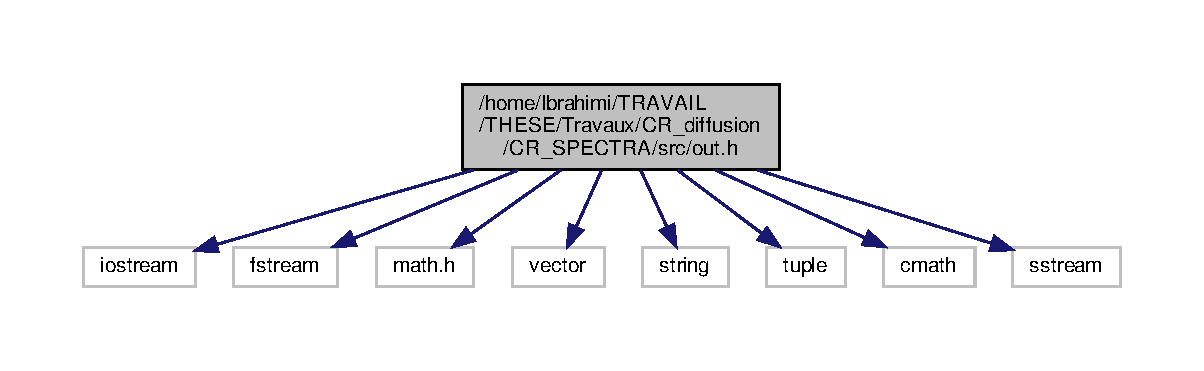
\includegraphics[width=350pt]{out_8h__incl}
\end{center}
\end{figure}
This graph shows which files directly or indirectly include this file\+:\nopagebreak
\begin{figure}[H]
\begin{center}
\leavevmode
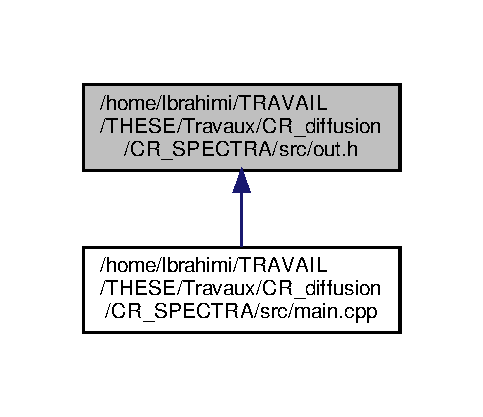
\includegraphics[width=232pt]{out_8h__dep__incl}
\end{center}
\end{figure}
\subsection*{Functions}
\begin{DoxyCompactItemize}
\item 
vector$<$ double $>$ \hyperlink{out_8h_a1b96bfc105db29caefe0dedd06daf16d}{specific\+Output\+Data} ()
\item 
vector$<$ double $>$ \hyperlink{out_8h_ae3f6312c6c9de7c2fbe83f8f4dde2428}{output\+Data} (double tmin, double tmax, int nvalues, string modulation, double eps)
\begin{DoxyCompactList}\small\item\em Output data function for a regular and large amount of output data. \end{DoxyCompactList}\item 
vector$<$ double $>$ \hyperlink{out_8h_a578da8858f46986d89cd97a6add06bed}{get\+Output} ()
\begin{DoxyCompactList}\small\item\em Main output file function. This one will be used in the main file. \end{DoxyCompactList}\item 
int \hyperlink{out_8h_a233e9761e7046e55da61cc72da9e03d6}{get\+Log\+Output} ()
\begin{DoxyCompactList}\small\item\em Main output log file function. This one will be used in the main file. \end{DoxyCompactList}\item 
double \hyperlink{out_8h_aca4e8ad8ce3ba51e2a640f6fd5beecac}{set\+Tmax} ()
\begin{DoxyCompactList}\small\item\em Define the limit time of your simulation. \end{DoxyCompactList}\end{DoxyCompactItemize}


\subsection{Function Documentation}
\mbox{\Hypertarget{out_8h_a233e9761e7046e55da61cc72da9e03d6}\label{out_8h_a233e9761e7046e55da61cc72da9e03d6}} 
\index{out.\+h@{out.\+h}!get\+Log\+Output@{get\+Log\+Output}}
\index{get\+Log\+Output@{get\+Log\+Output}!out.\+h@{out.\+h}}
\subsubsection{\texorpdfstring{get\+Log\+Output()}{getLogOutput()}}
{\footnotesize\ttfamily int get\+Log\+Output (\begin{DoxyParamCaption}{ }\end{DoxyParamCaption})}



Main output log file function. This one will be used in the main file. 

\mbox{\Hypertarget{out_8h_a578da8858f46986d89cd97a6add06bed}\label{out_8h_a578da8858f46986d89cd97a6add06bed}} 
\index{out.\+h@{out.\+h}!get\+Output@{get\+Output}}
\index{get\+Output@{get\+Output}!out.\+h@{out.\+h}}
\subsubsection{\texorpdfstring{get\+Output()}{getOutput()}}
{\footnotesize\ttfamily vector$<$double$>$ get\+Output (\begin{DoxyParamCaption}{ }\end{DoxyParamCaption})}



Main output file function. This one will be used in the main file. 

\mbox{\Hypertarget{out_8h_ae3f6312c6c9de7c2fbe83f8f4dde2428}\label{out_8h_ae3f6312c6c9de7c2fbe83f8f4dde2428}} 
\index{out.\+h@{out.\+h}!output\+Data@{output\+Data}}
\index{output\+Data@{output\+Data}!out.\+h@{out.\+h}}
\subsubsection{\texorpdfstring{output\+Data()}{outputData()}}
{\footnotesize\ttfamily vector$<$double$>$ output\+Data (\begin{DoxyParamCaption}\item[{double}]{tmin,  }\item[{double}]{tmax,  }\item[{int}]{nvalues,  }\item[{string}]{modulation,  }\item[{double}]{eps }\end{DoxyParamCaption})}



Output data function for a regular and large amount of output data. 

\mbox{\Hypertarget{out_8h_aca4e8ad8ce3ba51e2a640f6fd5beecac}\label{out_8h_aca4e8ad8ce3ba51e2a640f6fd5beecac}} 
\index{out.\+h@{out.\+h}!set\+Tmax@{set\+Tmax}}
\index{set\+Tmax@{set\+Tmax}!out.\+h@{out.\+h}}
\subsubsection{\texorpdfstring{set\+Tmax()}{setTmax()}}
{\footnotesize\ttfamily double set\+Tmax (\begin{DoxyParamCaption}{ }\end{DoxyParamCaption})}



Define the limit time of your simulation. 

\mbox{\Hypertarget{out_8h_a1b96bfc105db29caefe0dedd06daf16d}\label{out_8h_a1b96bfc105db29caefe0dedd06daf16d}} 
\index{out.\+h@{out.\+h}!specific\+Output\+Data@{specific\+Output\+Data}}
\index{specific\+Output\+Data@{specific\+Output\+Data}!out.\+h@{out.\+h}}
\subsubsection{\texorpdfstring{specific\+Output\+Data()}{specificOutputData()}}
{\footnotesize\ttfamily vector$<$double$>$ specific\+Output\+Data (\begin{DoxyParamCaption}{ }\end{DoxyParamCaption})}

This function allows you to specify your own data output time array You just need to fill the list loc\+\_\+data, example\+: double loc\+\_\+data\mbox{[}\mbox{]} = \{t1, t2, ..., tn\}; where t\+\_\+i is in seconds 
\hypertarget{read2D_8h}{}\section{/home/lbrahimi/\+T\+R\+A\+V\+A\+I\+L/\+T\+H\+E\+S\+E/\+Travaux/\+C\+R\+\_\+diffusion/\+C\+R\+\_\+\+S\+P\+E\+C\+T\+R\+A/src/read2D.h File Reference}
\label{read2D_8h}\index{/home/lbrahimi/\+T\+R\+A\+V\+A\+I\+L/\+T\+H\+E\+S\+E/\+Travaux/\+C\+R\+\_\+diffusion/\+C\+R\+\_\+\+S\+P\+E\+C\+T\+R\+A/src/read2\+D.\+h@{/home/lbrahimi/\+T\+R\+A\+V\+A\+I\+L/\+T\+H\+E\+S\+E/\+Travaux/\+C\+R\+\_\+diffusion/\+C\+R\+\_\+\+S\+P\+E\+C\+T\+R\+A/src/read2\+D.\+h}}
{\ttfamily \#include $<$string$>$}\newline
{\ttfamily \#include $<$vector$>$}\newline
{\ttfamily \#include $<$sstream$>$}\newline
{\ttfamily \#include $<$iostream$>$}\newline
{\ttfamily \#include $<$fstream$>$}\newline
Include dependency graph for read2\+D.\+h\+:\nopagebreak
\begin{figure}[H]
\begin{center}
\leavevmode
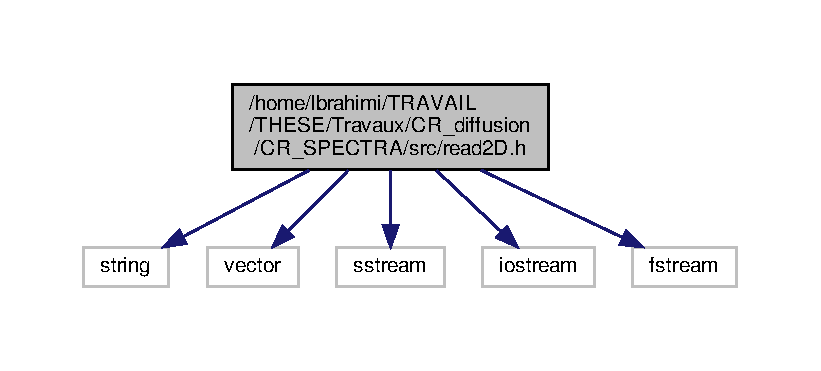
\includegraphics[width=350pt]{read2D_8h__incl}
\end{center}
\end{figure}
This graph shows which files directly or indirectly include this file\+:\nopagebreak
\begin{figure}[H]
\begin{center}
\leavevmode
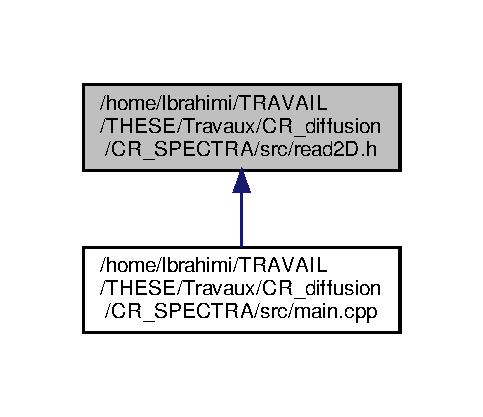
\includegraphics[width=232pt]{read2D_8h__dep__incl}
\end{center}
\end{figure}
\subsection*{Functions}
\begin{DoxyCompactItemize}
\item 
vector$<$ vector$<$ double $>$ $>$ \hyperlink{read2D_8h_ae34789b216c0e193eb18be6b35424647}{parse2\+D\+Csv\+File} (string input\+File\+Name, int start)
\end{DoxyCompactItemize}


\subsection{Function Documentation}
\mbox{\Hypertarget{read2D_8h_ae34789b216c0e193eb18be6b35424647}\label{read2D_8h_ae34789b216c0e193eb18be6b35424647}} 
\index{read2\+D.\+h@{read2\+D.\+h}!parse2\+D\+Csv\+File@{parse2\+D\+Csv\+File}}
\index{parse2\+D\+Csv\+File@{parse2\+D\+Csv\+File}!read2\+D.\+h@{read2\+D.\+h}}
\subsubsection{\texorpdfstring{parse2\+D\+Csv\+File()}{parse2DCsvFile()}}
{\footnotesize\ttfamily vector$<$vector$<$double$>$ $>$ parse2\+D\+Csv\+File (\begin{DoxyParamCaption}\item[{string}]{input\+File\+Name,  }\item[{int}]{start }\end{DoxyParamCaption})}

Reads csv file into table, exported as a vector of vector of doubles. 
\begin{DoxyParams}{Parameters}
{\em input\+File\+Name} & input file name (full path). \\
\hline
\end{DoxyParams}
\begin{DoxyReturn}{Returns}
data as vector of vector of doubles. 
\end{DoxyReturn}

\hypertarget{solver1D_8h}{}\section{/home/lbrahimi/\+T\+R\+A\+V\+A\+I\+L/\+T\+H\+E\+S\+E/\+Travaux/\+C\+R\+\_\+diffusion/\+C\+R\+\_\+\+S\+P\+E\+C\+T\+R\+A/src/solver1D.h File Reference}
\label{solver1D_8h}\index{/home/lbrahimi/\+T\+R\+A\+V\+A\+I\+L/\+T\+H\+E\+S\+E/\+Travaux/\+C\+R\+\_\+diffusion/\+C\+R\+\_\+\+S\+P\+E\+C\+T\+R\+A/src/solver1\+D.\+h@{/home/lbrahimi/\+T\+R\+A\+V\+A\+I\+L/\+T\+H\+E\+S\+E/\+Travaux/\+C\+R\+\_\+diffusion/\+C\+R\+\_\+\+S\+P\+E\+C\+T\+R\+A/src/solver1\+D.\+h}}
{\ttfamily \#include $<$iostream$>$}\newline
{\ttfamily \#include $<$fstream$>$}\newline
{\ttfamily \#include $<$math.\+h$>$}\newline
{\ttfamily \#include $<$vector$>$}\newline
{\ttfamily \#include $<$string$>$}\newline
{\ttfamily \#include $<$tuple$>$}\newline
{\ttfamily \#include $<$cmath$>$}\newline
{\ttfamily \#include $<$sstream$>$}\newline
Include dependency graph for solver1\+D.\+h\+:\nopagebreak
\begin{figure}[H]
\begin{center}
\leavevmode
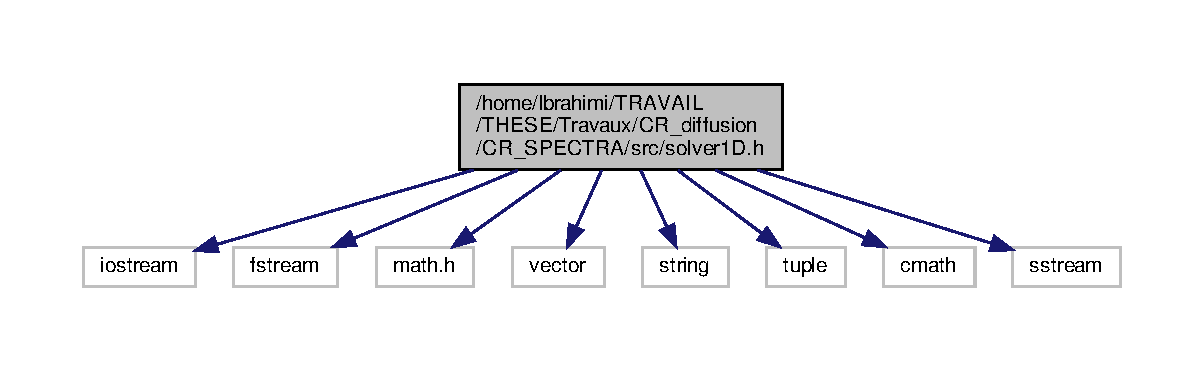
\includegraphics[width=350pt]{solver1D_8h__incl}
\end{center}
\end{figure}
This graph shows which files directly or indirectly include this file\+:\nopagebreak
\begin{figure}[H]
\begin{center}
\leavevmode
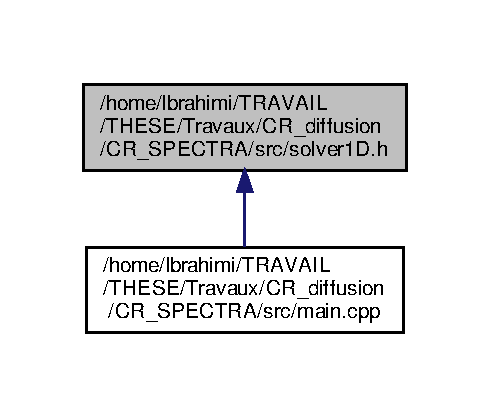
\includegraphics[width=235pt]{solver1D_8h__dep__incl}
\end{center}
\end{figure}
\subsection*{Functions}
\begin{DoxyCompactItemize}
\item 
void \hyperlink{solver1D_8h_afcb5a4e38370f967f2b945c0241f1831}{theta\+Diffusion\+Solver} (vector$<$ vector$<$ double $>$ $>$ \&u, vector$<$ vector$<$ double $>$ $>$ \&Pcr\+\_\+new, double dt, vector$<$ double $>$ X, int NE, vector$<$ vector$<$ double $>$ $>$ Ip, vector$<$ vector$<$ double $>$ $>$ Im, vector$<$ vector$<$ double $>$ $>$ Db, vector$<$ vector$<$ double $>$ $>$ \&Pcr\+\_\+background)
\item 
void \hyperlink{solver1D_8h_a103dc2e6463ef76cf14e9d242acc937c}{advection\+SolverX} (vector$<$ vector$<$ double $>$ $>$ \&u\+\_\+old, vector$<$ vector$<$ double $>$ $>$ \&u\+\_\+new, double dt, vector$<$ double $>$ X, int NE, vector$<$ vector$<$ double $>$ $>$ V, int sign, int border)
\item 
void \hyperlink{solver1D_8h_a48de9b2868ed9d20a5768f893eefb8c5}{advection\+SolverE} (vector$<$ vector$<$ double $>$ $>$ \&u\+\_\+old, vector$<$ vector$<$ double $>$ $>$ \&u\+\_\+new, double dt, vector$<$ double $>$ E, int NX, vector$<$ vector$<$ double $>$ $>$ V, vector$<$ vector$<$ double $>$ $>$ u\+\_\+background)
\item 
void \hyperlink{solver1D_8h_a106132d9d8efb08eab4d5cc10732620f}{advection\+Solver\+E1} (vector$<$ vector$<$ double $>$ $>$ \&u\+\_\+old, vector$<$ vector$<$ double $>$ $>$ \&u\+\_\+new, double dt, vector$<$ double $>$ E, vector$<$ double $>$ BB, vector$<$ double $>$ EE, int NX, vector$<$ vector$<$ double $>$ $>$ u\+\_\+background)
\item 
void \hyperlink{solver1D_8h_ad1d8d3c439326c4b5cafabb87f11562e}{advection\+Solver\+E2} (vector$<$ vector$<$ double $>$ $>$ \&u\+\_\+old, vector$<$ vector$<$ double $>$ $>$ \&u\+\_\+new, double dt, vector$<$ double $>$ E, int NX, vector$<$ double $>$ BB, vector$<$ double $>$ EE, vector$<$ vector$<$ double $>$ $>$ u\+\_\+background)
\item 
void \hyperlink{solver1D_8h_ad33fb869cbb96f9d08b1bccf86826fb1}{source\+Solver} (vector$<$ vector$<$ double $>$ $>$ \&u\+\_\+old, vector$<$ vector$<$ double $>$ $>$ \&u\+\_\+new, double dt, vector$<$ vector$<$ double $>$ $>$ source, double factor)
\item 
void \hyperlink{solver1D_8h_aa7f6eee49e4e9230307871dcb2d5a352}{source\+Growth\+Damp\+Rate\+Solver} (vector$<$ vector$<$ double $>$ $>$ \&u\+\_\+old, vector$<$ vector$<$ double $>$ $>$ \&u\+\_\+new, vector$<$ vector$<$ double $>$ $>$ v\+\_\+old, vector$<$ vector$<$ double $>$ $>$ source, vector$<$ vector$<$ double $>$ $>$ background, vector$<$ double $>$ X, double dt, vector$<$ vector$<$ double $>$ $>$ V, vector$<$ double $>$ B, int factor)
\item 
void \hyperlink{solver1D_8h_a2f8fd5ea7c6a1ef2468bf631f29dab6d}{C\+Rs\+Injection\+Source\+Solver} (vector$<$ vector$<$ double $>$ $>$ \&u\+\_\+old, vector$<$ vector$<$ double $>$ $>$ \&u\+\_\+new, double dt, vector$<$ double $>$ \hyperlink{cr__source_8h_ac19e2251663c1020061917ef7c2ce4cb}{Pcr\+\_\+ini}, vector$<$ double $>$ Finj\+\_\+temp, vector$<$ double $>$ vec\+\_\+theta)
\item 
void \hyperlink{solver1D_8h_a7131dd1fd5ac463bce6bf78177d87e2d}{dilute\+\_\+solver} (vector$<$ vector$<$ double $>$ $>$ \&u\+\_\+old, vector$<$ vector$<$ double $>$ $>$ \&u\+\_\+new, vector$<$ vector$<$ double $>$ $>$ u\+\_\+background, double r\+\_\+new, double r\+\_\+old, vector$<$ double $>$ nn, vector$<$ double $>$ \hyperlink{cr__source_8h_ad3975adf480fdb09e1ea14b1efa617e0}{ni}, vector$<$ double $>$ \hyperlink{constants_8h_affd3595ea3bf442893a3dc5bf568a663}{mn}, vector$<$ double $>$ mi, vector$<$ double $>$ B, vector$<$ double $>$ \hyperlink{cr__source_8h_ac94a6e5794c2d7b59588b14025cfba20}{T})
\item 
void \hyperlink{solver1D_8h_ae1556e55b3ed7913a25cb2323bb371f1}{perpendicular\+\_\+diffusion\+\_\+solver} (vector$<$ vector$<$ double $>$ $>$ \&u\+\_\+old, vector$<$ vector$<$ double $>$ $>$ \&u\+\_\+new, vector$<$ vector$<$ double $>$ $>$ u\+\_\+bc, vector$<$ vector$<$ double $>$ $>$ Db, vector$<$ vector$<$ double $>$ $>$ I0, vector$<$ double $>$ X, double dt, vector$<$ double $>$ r\+\_\+esc)
\item 
void \hyperlink{solver1D_8h_a6417f41d1afa5d62b6f1443fe545c586}{Not\+Move} (vector$<$ vector$<$ double $>$ $>$ u, vector$<$ vector$<$ double $>$ $>$ u\+\_\+new)
\item 
void \hyperlink{solver1D_8h_ad0d64194db46f0bbe65d9835903f1041}{electron\+\_\+source} (vector$<$ vector$<$ double $>$ $>$ \&u\+\_\+old, vector$<$ vector$<$ double $>$ $>$ \&u\+\_\+new, vector$<$ double $>$ E, double dt, int NE, int NX, vector$<$ vector$<$ double $>$ $>$ u\+\_\+background)
\end{DoxyCompactItemize}


\subsection{Function Documentation}
\mbox{\Hypertarget{solver1D_8h_a48de9b2868ed9d20a5768f893eefb8c5}\label{solver1D_8h_a48de9b2868ed9d20a5768f893eefb8c5}} 
\index{solver1\+D.\+h@{solver1\+D.\+h}!advection\+SolverE@{advection\+SolverE}}
\index{advection\+SolverE@{advection\+SolverE}!solver1\+D.\+h@{solver1\+D.\+h}}
\subsubsection{\texorpdfstring{advection\+Solver\+E()}{advectionSolverE()}}
{\footnotesize\ttfamily void advection\+SolverE (\begin{DoxyParamCaption}\item[{vector$<$ vector$<$ double $>$ $>$ \&}]{u\+\_\+old,  }\item[{vector$<$ vector$<$ double $>$ $>$ \&}]{u\+\_\+new,  }\item[{double}]{dt,  }\item[{vector$<$ double $>$}]{E,  }\item[{int}]{NX,  }\item[{vector$<$ vector$<$ double $>$ $>$}]{V,  }\item[{vector$<$ vector$<$ double $>$ $>$}]{u\+\_\+background }\end{DoxyParamCaption})}

\mbox{\Hypertarget{solver1D_8h_a106132d9d8efb08eab4d5cc10732620f}\label{solver1D_8h_a106132d9d8efb08eab4d5cc10732620f}} 
\index{solver1\+D.\+h@{solver1\+D.\+h}!advection\+Solver\+E1@{advection\+Solver\+E1}}
\index{advection\+Solver\+E1@{advection\+Solver\+E1}!solver1\+D.\+h@{solver1\+D.\+h}}
\subsubsection{\texorpdfstring{advection\+Solver\+E1()}{advectionSolverE1()}}
{\footnotesize\ttfamily void advection\+Solver\+E1 (\begin{DoxyParamCaption}\item[{vector$<$ vector$<$ double $>$ $>$ \&}]{u\+\_\+old,  }\item[{vector$<$ vector$<$ double $>$ $>$ \&}]{u\+\_\+new,  }\item[{double}]{dt,  }\item[{vector$<$ double $>$}]{E,  }\item[{vector$<$ double $>$}]{BB,  }\item[{vector$<$ double $>$}]{EE,  }\item[{int}]{NX,  }\item[{vector$<$ vector$<$ double $>$ $>$}]{u\+\_\+background }\end{DoxyParamCaption})}

\mbox{\Hypertarget{solver1D_8h_ad1d8d3c439326c4b5cafabb87f11562e}\label{solver1D_8h_ad1d8d3c439326c4b5cafabb87f11562e}} 
\index{solver1\+D.\+h@{solver1\+D.\+h}!advection\+Solver\+E2@{advection\+Solver\+E2}}
\index{advection\+Solver\+E2@{advection\+Solver\+E2}!solver1\+D.\+h@{solver1\+D.\+h}}
\subsubsection{\texorpdfstring{advection\+Solver\+E2()}{advectionSolverE2()}}
{\footnotesize\ttfamily void advection\+Solver\+E2 (\begin{DoxyParamCaption}\item[{vector$<$ vector$<$ double $>$ $>$ \&}]{u\+\_\+old,  }\item[{vector$<$ vector$<$ double $>$ $>$ \&}]{u\+\_\+new,  }\item[{double}]{dt,  }\item[{vector$<$ double $>$}]{E,  }\item[{int}]{NX,  }\item[{vector$<$ double $>$}]{BB,  }\item[{vector$<$ double $>$}]{EE,  }\item[{vector$<$ vector$<$ double $>$ $>$}]{u\+\_\+background }\end{DoxyParamCaption})}

\mbox{\Hypertarget{solver1D_8h_a103dc2e6463ef76cf14e9d242acc937c}\label{solver1D_8h_a103dc2e6463ef76cf14e9d242acc937c}} 
\index{solver1\+D.\+h@{solver1\+D.\+h}!advection\+SolverX@{advection\+SolverX}}
\index{advection\+SolverX@{advection\+SolverX}!solver1\+D.\+h@{solver1\+D.\+h}}
\subsubsection{\texorpdfstring{advection\+Solver\+X()}{advectionSolverX()}}
{\footnotesize\ttfamily void advection\+SolverX (\begin{DoxyParamCaption}\item[{vector$<$ vector$<$ double $>$ $>$ \&}]{u\+\_\+old,  }\item[{vector$<$ vector$<$ double $>$ $>$ \&}]{u\+\_\+new,  }\item[{double}]{dt,  }\item[{vector$<$ double $>$}]{X,  }\item[{int}]{NE,  }\item[{vector$<$ vector$<$ double $>$ $>$}]{V,  }\item[{int}]{sign,  }\item[{int}]{border }\end{DoxyParamCaption})}

\mbox{\Hypertarget{solver1D_8h_a2f8fd5ea7c6a1ef2468bf631f29dab6d}\label{solver1D_8h_a2f8fd5ea7c6a1ef2468bf631f29dab6d}} 
\index{solver1\+D.\+h@{solver1\+D.\+h}!C\+Rs\+Injection\+Source\+Solver@{C\+Rs\+Injection\+Source\+Solver}}
\index{C\+Rs\+Injection\+Source\+Solver@{C\+Rs\+Injection\+Source\+Solver}!solver1\+D.\+h@{solver1\+D.\+h}}
\subsubsection{\texorpdfstring{C\+Rs\+Injection\+Source\+Solver()}{CRsInjectionSourceSolver()}}
{\footnotesize\ttfamily void C\+Rs\+Injection\+Source\+Solver (\begin{DoxyParamCaption}\item[{vector$<$ vector$<$ double $>$ $>$ \&}]{u\+\_\+old,  }\item[{vector$<$ vector$<$ double $>$ $>$ \&}]{u\+\_\+new,  }\item[{double}]{dt,  }\item[{vector$<$ double $>$}]{Pcr\+\_\+ini,  }\item[{vector$<$ double $>$}]{Finj\+\_\+temp,  }\item[{vector$<$ double $>$}]{vec\+\_\+theta }\end{DoxyParamCaption})}

\mbox{\Hypertarget{solver1D_8h_a7131dd1fd5ac463bce6bf78177d87e2d}\label{solver1D_8h_a7131dd1fd5ac463bce6bf78177d87e2d}} 
\index{solver1\+D.\+h@{solver1\+D.\+h}!dilute\+\_\+solver@{dilute\+\_\+solver}}
\index{dilute\+\_\+solver@{dilute\+\_\+solver}!solver1\+D.\+h@{solver1\+D.\+h}}
\subsubsection{\texorpdfstring{dilute\+\_\+solver()}{dilute\_solver()}}
{\footnotesize\ttfamily void dilute\+\_\+solver (\begin{DoxyParamCaption}\item[{vector$<$ vector$<$ double $>$ $>$ \&}]{u\+\_\+old,  }\item[{vector$<$ vector$<$ double $>$ $>$ \&}]{u\+\_\+new,  }\item[{vector$<$ vector$<$ double $>$ $>$}]{u\+\_\+background,  }\item[{double}]{r\+\_\+new,  }\item[{double}]{r\+\_\+old,  }\item[{vector$<$ double $>$}]{nn,  }\item[{vector$<$ double $>$}]{ni,  }\item[{vector$<$ double $>$}]{mn,  }\item[{vector$<$ double $>$}]{mi,  }\item[{vector$<$ double $>$}]{B,  }\item[{vector$<$ double $>$}]{T }\end{DoxyParamCaption})}

\mbox{\Hypertarget{solver1D_8h_ad0d64194db46f0bbe65d9835903f1041}\label{solver1D_8h_ad0d64194db46f0bbe65d9835903f1041}} 
\index{solver1\+D.\+h@{solver1\+D.\+h}!electron\+\_\+source@{electron\+\_\+source}}
\index{electron\+\_\+source@{electron\+\_\+source}!solver1\+D.\+h@{solver1\+D.\+h}}
\subsubsection{\texorpdfstring{electron\+\_\+source()}{electron\_source()}}
{\footnotesize\ttfamily void electron\+\_\+source (\begin{DoxyParamCaption}\item[{vector$<$ vector$<$ double $>$ $>$ \&}]{u\+\_\+old,  }\item[{vector$<$ vector$<$ double $>$ $>$ \&}]{u\+\_\+new,  }\item[{vector$<$ double $>$}]{E,  }\item[{double}]{dt,  }\item[{int}]{NE,  }\item[{int}]{NX,  }\item[{vector$<$ vector$<$ double $>$ $>$}]{u\+\_\+background }\end{DoxyParamCaption})}

\mbox{\Hypertarget{solver1D_8h_a6417f41d1afa5d62b6f1443fe545c586}\label{solver1D_8h_a6417f41d1afa5d62b6f1443fe545c586}} 
\index{solver1\+D.\+h@{solver1\+D.\+h}!Not\+Move@{Not\+Move}}
\index{Not\+Move@{Not\+Move}!solver1\+D.\+h@{solver1\+D.\+h}}
\subsubsection{\texorpdfstring{Not\+Move()}{NotMove()}}
{\footnotesize\ttfamily void Not\+Move (\begin{DoxyParamCaption}\item[{vector$<$ vector$<$ double $>$ $>$}]{u,  }\item[{vector$<$ vector$<$ double $>$ $>$}]{u\+\_\+new }\end{DoxyParamCaption})}

\mbox{\Hypertarget{solver1D_8h_ae1556e55b3ed7913a25cb2323bb371f1}\label{solver1D_8h_ae1556e55b3ed7913a25cb2323bb371f1}} 
\index{solver1\+D.\+h@{solver1\+D.\+h}!perpendicular\+\_\+diffusion\+\_\+solver@{perpendicular\+\_\+diffusion\+\_\+solver}}
\index{perpendicular\+\_\+diffusion\+\_\+solver@{perpendicular\+\_\+diffusion\+\_\+solver}!solver1\+D.\+h@{solver1\+D.\+h}}
\subsubsection{\texorpdfstring{perpendicular\+\_\+diffusion\+\_\+solver()}{perpendicular\_diffusion\_solver()}}
{\footnotesize\ttfamily void perpendicular\+\_\+diffusion\+\_\+solver (\begin{DoxyParamCaption}\item[{vector$<$ vector$<$ double $>$ $>$ \&}]{u\+\_\+old,  }\item[{vector$<$ vector$<$ double $>$ $>$ \&}]{u\+\_\+new,  }\item[{vector$<$ vector$<$ double $>$ $>$}]{u\+\_\+bc,  }\item[{vector$<$ vector$<$ double $>$ $>$}]{Db,  }\item[{vector$<$ vector$<$ double $>$ $>$}]{I0,  }\item[{vector$<$ double $>$}]{X,  }\item[{double}]{dt,  }\item[{vector$<$ double $>$}]{r\+\_\+esc }\end{DoxyParamCaption})}

\mbox{\Hypertarget{solver1D_8h_aa7f6eee49e4e9230307871dcb2d5a352}\label{solver1D_8h_aa7f6eee49e4e9230307871dcb2d5a352}} 
\index{solver1\+D.\+h@{solver1\+D.\+h}!source\+Growth\+Damp\+Rate\+Solver@{source\+Growth\+Damp\+Rate\+Solver}}
\index{source\+Growth\+Damp\+Rate\+Solver@{source\+Growth\+Damp\+Rate\+Solver}!solver1\+D.\+h@{solver1\+D.\+h}}
\subsubsection{\texorpdfstring{source\+Growth\+Damp\+Rate\+Solver()}{sourceGrowthDampRateSolver()}}
{\footnotesize\ttfamily void source\+Growth\+Damp\+Rate\+Solver (\begin{DoxyParamCaption}\item[{vector$<$ vector$<$ double $>$ $>$ \&}]{u\+\_\+old,  }\item[{vector$<$ vector$<$ double $>$ $>$ \&}]{u\+\_\+new,  }\item[{vector$<$ vector$<$ double $>$ $>$}]{v\+\_\+old,  }\item[{vector$<$ vector$<$ double $>$ $>$}]{source,  }\item[{vector$<$ vector$<$ double $>$ $>$}]{background,  }\item[{vector$<$ double $>$}]{X,  }\item[{double}]{dt,  }\item[{vector$<$ vector$<$ double $>$ $>$}]{V,  }\item[{vector$<$ double $>$}]{B,  }\item[{int}]{factor }\end{DoxyParamCaption})}

\mbox{\Hypertarget{solver1D_8h_ad33fb869cbb96f9d08b1bccf86826fb1}\label{solver1D_8h_ad33fb869cbb96f9d08b1bccf86826fb1}} 
\index{solver1\+D.\+h@{solver1\+D.\+h}!source\+Solver@{source\+Solver}}
\index{source\+Solver@{source\+Solver}!solver1\+D.\+h@{solver1\+D.\+h}}
\subsubsection{\texorpdfstring{source\+Solver()}{sourceSolver()}}
{\footnotesize\ttfamily void source\+Solver (\begin{DoxyParamCaption}\item[{vector$<$ vector$<$ double $>$ $>$ \&}]{u\+\_\+old,  }\item[{vector$<$ vector$<$ double $>$ $>$ \&}]{u\+\_\+new,  }\item[{double}]{dt,  }\item[{vector$<$ vector$<$ double $>$ $>$}]{source,  }\item[{double}]{factor }\end{DoxyParamCaption})}

\mbox{\Hypertarget{solver1D_8h_afcb5a4e38370f967f2b945c0241f1831}\label{solver1D_8h_afcb5a4e38370f967f2b945c0241f1831}} 
\index{solver1\+D.\+h@{solver1\+D.\+h}!theta\+Diffusion\+Solver@{theta\+Diffusion\+Solver}}
\index{theta\+Diffusion\+Solver@{theta\+Diffusion\+Solver}!solver1\+D.\+h@{solver1\+D.\+h}}
\subsubsection{\texorpdfstring{theta\+Diffusion\+Solver()}{thetaDiffusionSolver()}}
{\footnotesize\ttfamily void theta\+Diffusion\+Solver (\begin{DoxyParamCaption}\item[{vector$<$ vector$<$ double $>$ $>$ \&}]{u,  }\item[{vector$<$ vector$<$ double $>$ $>$ \&}]{Pcr\+\_\+new,  }\item[{double}]{dt,  }\item[{vector$<$ double $>$}]{X,  }\item[{int}]{NE,  }\item[{vector$<$ vector$<$ double $>$ $>$}]{Ip,  }\item[{vector$<$ vector$<$ double $>$ $>$}]{Im,  }\item[{vector$<$ vector$<$ double $>$ $>$}]{Db,  }\item[{vector$<$ vector$<$ double $>$ $>$ \&}]{Pcr\+\_\+background }\end{DoxyParamCaption})}


\hypertarget{tools_8h}{}\section{/home/lbrahimi/\+T\+R\+A\+V\+A\+I\+L/\+T\+H\+E\+S\+E/\+Travaux/\+C\+R\+\_\+diffusion/\+C\+R\+\_\+\+S\+P\+E\+C\+T\+R\+A/src/tools.h File Reference}
\label{tools_8h}\index{/home/lbrahimi/\+T\+R\+A\+V\+A\+I\+L/\+T\+H\+E\+S\+E/\+Travaux/\+C\+R\+\_\+diffusion/\+C\+R\+\_\+\+S\+P\+E\+C\+T\+R\+A/src/tools.\+h@{/home/lbrahimi/\+T\+R\+A\+V\+A\+I\+L/\+T\+H\+E\+S\+E/\+Travaux/\+C\+R\+\_\+diffusion/\+C\+R\+\_\+\+S\+P\+E\+C\+T\+R\+A/src/tools.\+h}}
{\ttfamily \#include $<$iostream$>$}\newline
{\ttfamily \#include $<$fstream$>$}\newline
{\ttfamily \#include $<$math.\+h$>$}\newline
{\ttfamily \#include $<$vector$>$}\newline
{\ttfamily \#include $<$string$>$}\newline
{\ttfamily \#include $<$tuple$>$}\newline
{\ttfamily \#include $<$cmath$>$}\newline
{\ttfamily \#include $<$sstream$>$}\newline
Include dependency graph for tools.\+h\+:\nopagebreak
\begin{figure}[H]
\begin{center}
\leavevmode
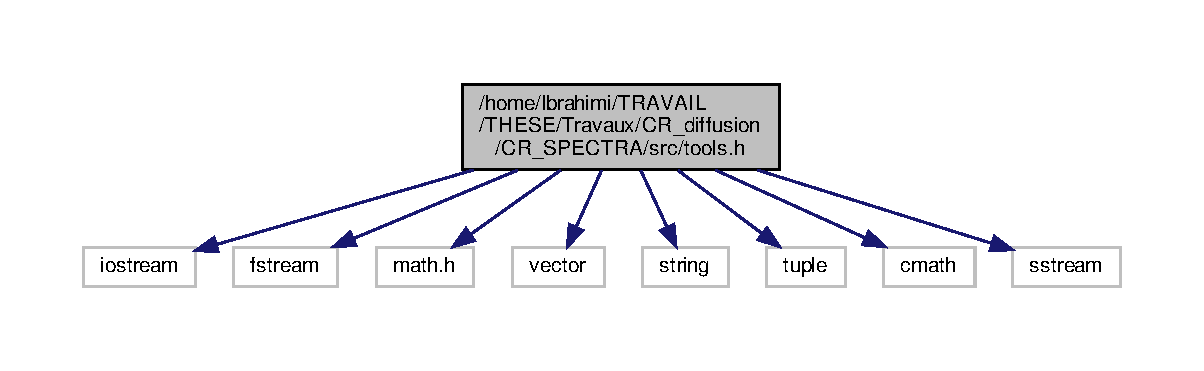
\includegraphics[width=350pt]{tools_8h__incl}
\end{center}
\end{figure}
This graph shows which files directly or indirectly include this file\+:\nopagebreak
\begin{figure}[H]
\begin{center}
\leavevmode
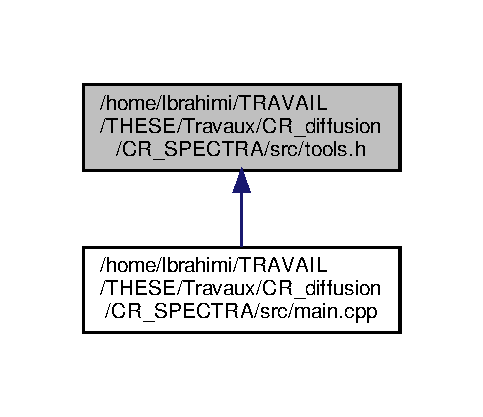
\includegraphics[width=232pt]{tools_8h__dep__incl}
\end{center}
\end{figure}
\subsection*{Functions}
\begin{DoxyCompactItemize}
\item 
double \hyperlink{tools_8h_aa042167510729213eb7a1448941cd319}{max\+Element1D} (vector$<$ double $>$ data)
\item 
double \hyperlink{tools_8h_ac1c46c33e34ac092a8149c2836750993}{min\+Element1D} (vector$<$ double $>$ data)
\item 
double \hyperlink{tools_8h_a6d2fa0dc0e404bdf0b1ee05638426750}{max\+Element2D} (vector$<$ vector$<$ double $>$ $>$ data)
\item 
double \hyperlink{tools_8h_a33f4f621ed13873f1165895d21b9deff}{min\+Element2D} (vector$<$ vector$<$ double $>$ $>$ data)
\item 
double \hyperlink{tools_8h_a5eaf5f0f2482d71c4b2bd0645faf32aa}{absmax\+Element2D} (vector$<$ vector$<$ double $>$ $>$ data)
\end{DoxyCompactItemize}


\subsection{Function Documentation}
\mbox{\Hypertarget{tools_8h_a5eaf5f0f2482d71c4b2bd0645faf32aa}\label{tools_8h_a5eaf5f0f2482d71c4b2bd0645faf32aa}} 
\index{tools.\+h@{tools.\+h}!absmax\+Element2D@{absmax\+Element2D}}
\index{absmax\+Element2D@{absmax\+Element2D}!tools.\+h@{tools.\+h}}
\subsubsection{\texorpdfstring{absmax\+Element2\+D()}{absmaxElement2D()}}
{\footnotesize\ttfamily double absmax\+Element2D (\begin{DoxyParamCaption}\item[{vector$<$ vector$<$ double $>$ $>$}]{data }\end{DoxyParamCaption})}

\mbox{\Hypertarget{tools_8h_aa042167510729213eb7a1448941cd319}\label{tools_8h_aa042167510729213eb7a1448941cd319}} 
\index{tools.\+h@{tools.\+h}!max\+Element1D@{max\+Element1D}}
\index{max\+Element1D@{max\+Element1D}!tools.\+h@{tools.\+h}}
\subsubsection{\texorpdfstring{max\+Element1\+D()}{maxElement1D()}}
{\footnotesize\ttfamily double max\+Element1D (\begin{DoxyParamCaption}\item[{vector$<$ double $>$}]{data }\end{DoxyParamCaption})}

\mbox{\Hypertarget{tools_8h_a6d2fa0dc0e404bdf0b1ee05638426750}\label{tools_8h_a6d2fa0dc0e404bdf0b1ee05638426750}} 
\index{tools.\+h@{tools.\+h}!max\+Element2D@{max\+Element2D}}
\index{max\+Element2D@{max\+Element2D}!tools.\+h@{tools.\+h}}
\subsubsection{\texorpdfstring{max\+Element2\+D()}{maxElement2D()}}
{\footnotesize\ttfamily double max\+Element2D (\begin{DoxyParamCaption}\item[{vector$<$ vector$<$ double $>$ $>$}]{data }\end{DoxyParamCaption})}

\mbox{\Hypertarget{tools_8h_ac1c46c33e34ac092a8149c2836750993}\label{tools_8h_ac1c46c33e34ac092a8149c2836750993}} 
\index{tools.\+h@{tools.\+h}!min\+Element1D@{min\+Element1D}}
\index{min\+Element1D@{min\+Element1D}!tools.\+h@{tools.\+h}}
\subsubsection{\texorpdfstring{min\+Element1\+D()}{minElement1D()}}
{\footnotesize\ttfamily double min\+Element1D (\begin{DoxyParamCaption}\item[{vector$<$ double $>$}]{data }\end{DoxyParamCaption})}

\mbox{\Hypertarget{tools_8h_a33f4f621ed13873f1165895d21b9deff}\label{tools_8h_a33f4f621ed13873f1165895d21b9deff}} 
\index{tools.\+h@{tools.\+h}!min\+Element2D@{min\+Element2D}}
\index{min\+Element2D@{min\+Element2D}!tools.\+h@{tools.\+h}}
\subsubsection{\texorpdfstring{min\+Element2\+D()}{minElement2D()}}
{\footnotesize\ttfamily double min\+Element2D (\begin{DoxyParamCaption}\item[{vector$<$ vector$<$ double $>$ $>$}]{data }\end{DoxyParamCaption})}


\hypertarget{background__diffusion__coefficient_8py}{}\section{/home/lbrahimi/\+T\+R\+A\+V\+A\+I\+L/\+T\+H\+E\+S\+E/\+Travaux/\+C\+R\+\_\+diffusion/\+C\+R\+\_\+\+S\+P\+E\+C\+T\+R\+A/tools/background\+\_\+diffusion\+\_\+coefficient.py File Reference}
\label{background__diffusion__coefficient_8py}\index{/home/lbrahimi/\+T\+R\+A\+V\+A\+I\+L/\+T\+H\+E\+S\+E/\+Travaux/\+C\+R\+\_\+diffusion/\+C\+R\+\_\+\+S\+P\+E\+C\+T\+R\+A/tools/background\+\_\+diffusion\+\_\+coefficient.\+py@{/home/lbrahimi/\+T\+R\+A\+V\+A\+I\+L/\+T\+H\+E\+S\+E/\+Travaux/\+C\+R\+\_\+diffusion/\+C\+R\+\_\+\+S\+P\+E\+C\+T\+R\+A/tools/background\+\_\+diffusion\+\_\+coefficient.\+py}}
\subsection*{Namespaces}
\begin{DoxyCompactItemize}
\item 
 \hyperlink{namespacebackground__diffusion__coefficient}{background\+\_\+diffusion\+\_\+coefficient}
\end{DoxyCompactItemize}
\subsection*{Functions}
\begin{DoxyCompactItemize}
\item 
def \hyperlink{namespacebackground__diffusion__coefficient_aebebdbdd7bf44f9ebd3485b6abe00093}{background\+\_\+diffusion\+\_\+coefficient.\+Ion\+Neutral\+\_\+\+Damping} (k, medium\+\_\+props, nu\+\_\+n=0, \hyperlink{cr__source_8h_a91a3bf9ce71325c8a7cbd31d8c474bff}{theta}=0)
\item 
def \hyperlink{namespacebackground__diffusion__coefficient_a98bcd7e8761c065f7586e89f4d9050c8}{background\+\_\+diffusion\+\_\+coefficient.\+Duu\+\_\+\+Alfven\+\_\+\+Slab\+\_\+\+Linear\+\_\+\+Undamped} (mu, E, medium\+\_\+props, mass=\hyperlink{constants_8h_a6b331c08a80ed71d31c55a3341776483}{cst.\+mp}, kmin=1e-\/20, q=1.\+5, I=1e-\/4)
\item 
def \hyperlink{namespacebackground__diffusion__coefficient_a90de23556ff1b6647c805b26e421a00f}{background\+\_\+diffusion\+\_\+coefficient.\+Kappa\+\_\+zz} (E, medium\+\_\+props, mass=\hyperlink{constants_8h_a6b331c08a80ed71d31c55a3341776483}{cst.\+mp}, kmin=(50.$\ast$\hyperlink{constants_8h_a2884cd030c4c825754349a525a1d06ce}{cst.\+pc}) $\ast$$\ast$(-\/1), q=5./3, I=1e-\/4)
\end{DoxyCompactItemize}

\hypertarget{show__models_2obsolette_2background__diffusion__coefficient_8py}{}\section{/home/lbrahimi/\+T\+R\+A\+V\+A\+I\+L/\+T\+H\+E\+S\+E/\+Travaux/\+C\+R\+\_\+diffusion/\+C\+R\+\_\+\+S\+P\+E\+C\+T\+R\+A/tools/show\+\_\+models/obsolette/background\+\_\+diffusion\+\_\+coefficient.py File Reference}
\label{show__models_2obsolette_2background__diffusion__coefficient_8py}\index{/home/lbrahimi/\+T\+R\+A\+V\+A\+I\+L/\+T\+H\+E\+S\+E/\+Travaux/\+C\+R\+\_\+diffusion/\+C\+R\+\_\+\+S\+P\+E\+C\+T\+R\+A/tools/show\+\_\+models/obsolette/background\+\_\+diffusion\+\_\+coefficient.\+py@{/home/lbrahimi/\+T\+R\+A\+V\+A\+I\+L/\+T\+H\+E\+S\+E/\+Travaux/\+C\+R\+\_\+diffusion/\+C\+R\+\_\+\+S\+P\+E\+C\+T\+R\+A/tools/show\+\_\+models/obsolette/background\+\_\+diffusion\+\_\+coefficient.\+py}}
\subsection*{Namespaces}
\begin{DoxyCompactItemize}
\item 
 \hyperlink{namespacebackground__diffusion__coefficient}{background\+\_\+diffusion\+\_\+coefficient}
\end{DoxyCompactItemize}
\subsection*{Functions}
\begin{DoxyCompactItemize}
\item 
def \hyperlink{namespacebackground__diffusion__coefficient_a751d44e9536ec7a83b768e7829c8ea95}{background\+\_\+diffusion\+\_\+coefficient.\+J} (a, b, \hyperlink{constants_8h_a8fc6defe4e499b1b9b9c275689e44352}{c}, D, q, x)
\end{DoxyCompactItemize}
\subsection*{Variables}
\begin{DoxyCompactItemize}
\item 
\hyperlink{namespacebackground__diffusion__coefficient_a20db986331b23bdcbf8aa70bee4dad81}{background\+\_\+diffusion\+\_\+coefficient.\+phase} = ism.\+C\+NM
\item 
\hyperlink{namespacebackground__diffusion__coefficient_aa4c740d378c977bba73862b678bc7aa8}{background\+\_\+diffusion\+\_\+coefficient.\+B0} = phase.\+get(\textquotesingle{}B\textquotesingle{})
\item 
\hyperlink{namespacebackground__diffusion__coefficient_a374568e409883fc9a7717e1bfd2e809c}{background\+\_\+diffusion\+\_\+coefficient.\+mi} = phase.\+get(\char`\"{}mi\char`\"{})
\item 
\hyperlink{namespacebackground__diffusion__coefficient_a51fdf68aec0a8c94efcb4cc3a8e0f25c}{background\+\_\+diffusion\+\_\+coefficient.\+mn} = phase.\+get(\char`\"{}mn\char`\"{})
\item 
\hyperlink{namespacebackground__diffusion__coefficient_af7412737bbcd1dfa68de3eb3094039c9}{background\+\_\+diffusion\+\_\+coefficient.\+ni} = phase.\+get(\char`\"{}ni\char`\"{})
\item 
\hyperlink{namespacebackground__diffusion__coefficient_a6a12435a1b17f24ec599317bd1d5df3e}{background\+\_\+diffusion\+\_\+coefficient.\+nn} = phase.\+get(\char`\"{}nn\char`\"{})
\item 
\hyperlink{namespacebackground__diffusion__coefficient_a1161329fa7e310f2fd222a00aa15fc58}{background\+\_\+diffusion\+\_\+coefficient.\+T} = phase.\+get(\char`\"{}T\char`\"{})
\item 
tuple \hyperlink{namespacebackground__diffusion__coefficient_a5e73e055f2d553775d30e56959e66f6a}{background\+\_\+diffusion\+\_\+coefficient.\+chi} = (\hyperlink{constants_8h_affd3595ea3bf442893a3dc5bf568a663}{mn}$\ast$nn)/(mi$\ast$\hyperlink{cr__source_8h_ad3975adf480fdb09e1ea14b1efa617e0}{ni})
\item 
\hyperlink{namespacebackground__diffusion__coefficient_a55ec72a6244c82e3b52d71275b87f943}{background\+\_\+diffusion\+\_\+coefficient.\+V\+Ai} = B0/np.\+sqrt(4$\ast$\hyperlink{constants_8h_a43016d873124d39034edb8cd164794db}{np.\+pi}$\ast$mi$\ast$\hyperlink{cr__source_8h_ad3975adf480fdb09e1ea14b1efa617e0}{ni})
\item 
\hyperlink{namespacebackground__diffusion__coefficient_ac633d9c84127aeb9f09cf992f56a04c5}{background\+\_\+diffusion\+\_\+coefficient.\+VA} = B0/np.\+sqrt(4$\ast$\hyperlink{constants_8h_a43016d873124d39034edb8cd164794db}{np.\+pi}$\ast$(mi$\ast$\hyperlink{cr__source_8h_ad3975adf480fdb09e1ea14b1efa617e0}{ni} + \hyperlink{constants_8h_affd3595ea3bf442893a3dc5bf568a663}{mn}$\ast$nn))
\item 
int \hyperlink{namespacebackground__diffusion__coefficient_af291e92fa0584b42b3534383c2e268cd}{background\+\_\+diffusion\+\_\+coefficient.\+nu\+\_\+in} = 2$\ast$nn$\ast$8.\+4e-\/9$\ast$(50/1e4)$\ast$$\ast$0.\+4
\item 
tuple \hyperlink{namespacebackground__diffusion__coefficient_a23d06f244d61e8a53b7539228ae44b27}{background\+\_\+diffusion\+\_\+coefficient.\+nu\+\_\+ni} = chi$\ast$$\ast$(-\/1.)$\ast$nu\+\_\+in
\item 
int \hyperlink{namespacebackground__diffusion__coefficient_a424b7ddec26265fff4b1c019cb53daf5}{background\+\_\+diffusion\+\_\+coefficient.\+k\+\_\+min} = 1e-\/20
\item 
int \hyperlink{namespacebackground__diffusion__coefficient_a2dc993ce2a57243c719d0b85744329fb}{background\+\_\+diffusion\+\_\+coefficient.\+k\+\_\+cm} = 1e-\/15
\item 
int \hyperlink{namespacebackground__diffusion__coefficient_a0a6acfaf54c5336eb102db480044d0c7}{background\+\_\+diffusion\+\_\+coefficient.\+k\+\_\+cp} = 1e-\/20
\item 
int \hyperlink{namespacebackground__diffusion__coefficient_ac69190c330c03d78adfb5fed3eb84f56}{background\+\_\+diffusion\+\_\+coefficient.\+k\+\_\+max} = 2$\ast$nu\+\_\+ni/VA
\item 
int \hyperlink{namespacebackground__diffusion__coefficient_a1d825f16046d1366622e80b27c5abe8f}{background\+\_\+diffusion\+\_\+coefficient.\+E} = 10$\ast$\hyperlink{constants_8h_aec0e126d9991db8ad0b26139f5860568}{cst.\+GeV}
\item 
\hyperlink{namespacebackground__diffusion__coefficient_a0b4d5494f0e9b052747450abad02659c}{background\+\_\+diffusion\+\_\+coefficient.\+m} = \hyperlink{constants_8h_a6b331c08a80ed71d31c55a3341776483}{cst.\+mp}
\item 
int \hyperlink{namespacebackground__diffusion__coefficient_a2514d67dd3e18da9856bd25e26c23a78}{background\+\_\+diffusion\+\_\+coefficient.\+gamma} = 1 + (E /(m$\ast$\hyperlink{constants_8h_a8fc6defe4e499b1b9b9c275689e44352}{cst.\+c}$\ast$$\ast$2))
\item 
\hyperlink{namespacebackground__diffusion__coefficient_ae9abae81fd1c7196ed03b7e5a0addbd2}{background\+\_\+diffusion\+\_\+coefficient.\+v} = \hyperlink{constants_8h_a8fc6defe4e499b1b9b9c275689e44352}{cst.\+c}$\ast$np.\+sqrt(1 -\/ (1/(E/(m$\ast$\hyperlink{constants_8h_a8fc6defe4e499b1b9b9c275689e44352}{cst.\+c}$\ast$$\ast$2) + 1))$\ast$$\ast$2)
\item 
int \hyperlink{namespacebackground__diffusion__coefficient_ac9fab323229e14a97b8f31610270ce26}{background\+\_\+diffusion\+\_\+coefficient.\+p} = gamma$\ast$m$\ast$v
\item 
\hyperlink{namespacebackground__diffusion__coefficient_a3822940ebf79a8b0f24d85fc964bfec3}{background\+\_\+diffusion\+\_\+coefficient.\+Omega0} = \hyperlink{constants_8h_a2b076531cd50c7b55702a53221f2ac72}{cst.\+e}$\ast$B0/(m$\ast$\hyperlink{constants_8h_a8fc6defe4e499b1b9b9c275689e44352}{cst.\+c})
\item 
int \hyperlink{namespacebackground__diffusion__coefficient_a01702f7bd5c02645ef1e1ffb9dd228f3}{background\+\_\+diffusion\+\_\+coefficient.\+Omega} = Omega0/gamma
\item 
\hyperlink{namespacebackground__diffusion__coefficient_aff54de3ac975c901763d9ead73135baf}{background\+\_\+diffusion\+\_\+coefficient.\+mu} = np.\+linspace(-\/0.\+99, 0.\+99, 100)
\item 
\hyperlink{namespacebackground__diffusion__coefficient_a07238e955bce87de4940bb113bfaea7f}{background\+\_\+diffusion\+\_\+coefficient.\+d\+\_\+uu} = np.\+zeros(len(mu))
\item 
int \hyperlink{namespacebackground__diffusion__coefficient_aca65f5f95e49ead9f7c9d7c46cf3b523}{background\+\_\+diffusion\+\_\+coefficient.\+k\+\_\+zz} = 0.
\item 
\hyperlink{namespacebackground__diffusion__coefficient_af59da0f86db3e10dce09c197dc2666ea}{background\+\_\+diffusion\+\_\+coefficient.\+dmu} = mu\mbox{[}1\mbox{]} -\/ mu\mbox{[}0\mbox{]}
\item 
int \hyperlink{namespacebackground__diffusion__coefficient_a285b9795e8d8acb7f86327172c532499}{background\+\_\+diffusion\+\_\+coefficient.\+Itot} = 1e-\/1
\item 
float \hyperlink{namespacebackground__diffusion__coefficient_a24c8ca7d427bce7fc5fffc26e51655c4}{background\+\_\+diffusion\+\_\+coefficient.\+q} = 1.\+5
\item 
tuple \hyperlink{namespacebackground__diffusion__coefficient_a136aa61656385e49855d586138d39374}{background\+\_\+diffusion\+\_\+coefficient.\+a} = (v$\ast$mu\mbox{[}ii\mbox{]} -\/ VA)$\ast$$\ast$2
\item 
int \hyperlink{namespacebackground__diffusion__coefficient_a1c03ac6c07803cd1cd40a72d62e554f8}{background\+\_\+diffusion\+\_\+coefficient.\+b} = 2$\ast$Omega$\ast$(v$\ast$mu\mbox{[}ii\mbox{]} -\/ VA)
\item 
int \hyperlink{namespacebackground__diffusion__coefficient_a01bae0e931fba5b49a75b9e7aace34eb}{background\+\_\+diffusion\+\_\+coefficient.\+c} = Omega$\ast$$\ast$2 + (-\/ nu\+\_\+in/2)$\ast$$\ast$2
\item 
int \hyperlink{namespacebackground__diffusion__coefficient_a49751c69870f10700f7e674b48ea1d7d}{background\+\_\+diffusion\+\_\+coefficient.\+D} = b$\ast$$\ast$2 -\/ 4$\ast$a$\ast$\hyperlink{constants_8h_a8fc6defe4e499b1b9b9c275689e44352}{c}
\item 
\hyperlink{namespacebackground__diffusion__coefficient_a4d1079db2ed52f0edb4338fb53d37273}{background\+\_\+diffusion\+\_\+coefficient.\+eps} = VA/v
\item 
int \hyperlink{namespacebackground__diffusion__coefficient_af3fa68a7befc04e0431349f8f93c397b}{background\+\_\+diffusion\+\_\+coefficient.\+gs0} = 2$\ast$(q-\/1)$\ast$(B0$\ast$$\ast$2/(8$\ast$\hyperlink{constants_8h_a43016d873124d39034edb8cd164794db}{np.\+pi}))$\ast$Itot$\ast$k\+\_\+cp$\ast$$\ast$(q -\/ 1)
\item 
def \hyperlink{namespacebackground__diffusion__coefficient_a32490e647c215710899520f476309006}{background\+\_\+diffusion\+\_\+coefficient.\+fj\+\_\+p} = J(a, b, \hyperlink{constants_8h_a8fc6defe4e499b1b9b9c275689e44352}{c}, D, q, k\+\_\+max) -\/ J(a, b, \hyperlink{constants_8h_a8fc6defe4e499b1b9b9c275689e44352}{c}, D, q, k\+\_\+cp)
\item 
def \hyperlink{namespacebackground__diffusion__coefficient_a462877ed2f8058608830a27d3857187b}{background\+\_\+diffusion\+\_\+coefficient.\+fj\+\_\+m} = J(a, -\/b, \hyperlink{constants_8h_a8fc6defe4e499b1b9b9c275689e44352}{c}, D, q, k\+\_\+max) -\/ J(a, -\/b, \hyperlink{constants_8h_a8fc6defe4e499b1b9b9c275689e44352}{c}, D, q, k\+\_\+cp)
\item 
int \hyperlink{namespacebackground__diffusion__coefficient_af732e0e9d46a756c465592e68f78dd2d}{background\+\_\+diffusion\+\_\+coefficient.\+I} = -\/2$\ast$gs0$\ast$(1 -\/ mu\mbox{[}ii\mbox{]}$\ast$eps)$\ast$$\ast$2$\ast$(-\/ nu\+\_\+in/2.)$\ast$fj\+\_\+p
\end{DoxyCompactItemize}

\hypertarget{constants_8py}{}\section{/home/lbrahimi/\+T\+R\+A\+V\+A\+I\+L/\+T\+H\+E\+S\+E/\+Travaux/\+C\+R\+\_\+diffusion/\+C\+R\+\_\+\+S\+P\+E\+C\+T\+R\+A/tools/constants.py File Reference}
\label{constants_8py}\index{/home/lbrahimi/\+T\+R\+A\+V\+A\+I\+L/\+T\+H\+E\+S\+E/\+Travaux/\+C\+R\+\_\+diffusion/\+C\+R\+\_\+\+S\+P\+E\+C\+T\+R\+A/tools/constants.\+py@{/home/lbrahimi/\+T\+R\+A\+V\+A\+I\+L/\+T\+H\+E\+S\+E/\+Travaux/\+C\+R\+\_\+diffusion/\+C\+R\+\_\+\+S\+P\+E\+C\+T\+R\+A/tools/constants.\+py}}
\subsection*{Namespaces}
\begin{DoxyCompactItemize}
\item 
 \hyperlink{namespaceconstants}{constants}
\end{DoxyCompactItemize}
\subsection*{Variables}
\begin{DoxyCompactItemize}
\item 
float \hyperlink{namespaceconstants_a14d775b1c17d869c0f0d447f0bfc9330}{constants.\+yr} = 3.\+154e+7
\item 
int \hyperlink{namespaceconstants_ab5bb5ac138ecb54ccd663804b1c3ab9c}{constants.\+kyr} = 1e3$\ast$yr
\item 
float \hyperlink{namespaceconstants_a93c63f6ed8c5e300d378f5e4007f9b6d}{constants.\+pc} = 3.\+086e18
\item 
int \hyperlink{namespaceconstants_ad91def68fa6a3afee415cc69061a7583}{constants.\+kpc} = 1.e3$\ast$\hyperlink{constants_8h_a2884cd030c4c825754349a525a1d06ce}{pc}
\item 
float \hyperlink{namespaceconstants_ae15025e47a0397f98ad31918b0c426d4}{constants.\+GeV} = 0.\+00160218
\item 
int \hyperlink{namespaceconstants_acfeca3926802be06862b690861b75547}{constants.\+TeV} = 1e3$\ast$\+GeV
\item 
float \hyperlink{namespaceconstants_a93953cf99166a4a0b70cf2daf5d08be5}{constants.\+eV} = \hyperlink{constants_8h_aec0e126d9991db8ad0b26139f5860568}{GeV}$\ast$1e-\/9
\item 
int \hyperlink{namespaceconstants_a833162acb0cb16acebd5e3379bb4ab4d}{constants.\+MeV} = 1e-\/3$\ast$\+GeV
\item 
float \hyperlink{namespaceconstants_a5103d84ddd0c3eff4199593db0a5d88d}{constants.\+me} = 9.\+10938e-\/28
\item 
float \hyperlink{namespaceconstants_aebdc70445dfb9e72960792ba2efe97ab}{constants.\+mp} = 1.\+6726219e-\/24
\item 
float \hyperlink{namespaceconstants_ad53f198771c37114065171d857217e26}{constants.\+mn} = 1.\+6749286e-\/24
\item 
float \hyperlink{namespaceconstants_a7eb320ffb8626bac1462d41ac52f4938}{constants.\+m\+HI} = \hyperlink{constants_8h_a6b331c08a80ed71d31c55a3341776483}{mp}
\item 
float \hyperlink{namespaceconstants_a8529868bbaabd3d0324f40286633083c}{constants.\+m\+H\+II} = \hyperlink{constants_8h_a6b331c08a80ed71d31c55a3341776483}{mp}
\item 
int \hyperlink{namespaceconstants_af49326d192aac38eba034ab6650bf4da}{constants.\+m\+HeI} = 2$\ast$\hyperlink{constants_8h_a6b331c08a80ed71d31c55a3341776483}{mp} + 2$\ast$\hyperlink{constants_8h_affd3595ea3bf442893a3dc5bf568a663}{mn}
\item 
int \hyperlink{namespaceconstants_abc800d0399d254c2a946705bfadf7c41}{constants.\+m\+He\+II} = 2$\ast$\hyperlink{constants_8h_a6b331c08a80ed71d31c55a3341776483}{mp} + 2$\ast$\hyperlink{constants_8h_affd3595ea3bf442893a3dc5bf568a663}{mn}
\item 
int \hyperlink{namespaceconstants_a4039b9e829bd537908aaf35345f3d434}{constants.\+m\+C\+II} = 6$\ast$\hyperlink{constants_8h_a6b331c08a80ed71d31c55a3341776483}{mp} + 6$\ast$\hyperlink{constants_8h_affd3595ea3bf442893a3dc5bf568a663}{mn}
\item 
int \hyperlink{namespaceconstants_a649f0308f09cf86c9658ebbddab3a4ce}{constants.\+m\+H\+C\+O\+II} = 8$\ast$\hyperlink{constants_8h_a6b331c08a80ed71d31c55a3341776483}{mp} + 8$\ast$\hyperlink{constants_8h_affd3595ea3bf442893a3dc5bf568a663}{mn} + 6$\ast$\hyperlink{constants_8h_a6b331c08a80ed71d31c55a3341776483}{mp} + 6$\ast$\hyperlink{constants_8h_affd3595ea3bf442893a3dc5bf568a663}{mn} + \hyperlink{constants_8h_a6b331c08a80ed71d31c55a3341776483}{mp} + \hyperlink{constants_8h_affd3595ea3bf442893a3dc5bf568a663}{mn}
\item 
int \hyperlink{namespaceconstants_a6286571f2bce388e5cba5df404f6a605}{constants.\+m\+H2} = 2$\ast$\hyperlink{constants_8h_a6b331c08a80ed71d31c55a3341776483}{mp}
\item 
float \hyperlink{namespaceconstants_a25294f89fd53b34a138ea616e9c0ccee}{constants.\+e} = 4.\+80326e-\/10
\item 
int \hyperlink{namespaceconstants_ae66e312a5fe9e01cf32156cf8f5528b3}{constants.\+c} = 29979245800.
\item 
float \hyperlink{namespaceconstants_a484db162dd0953d02cc095d9e0fd90e5}{constants.\+kbolz} = 1.\+3807e-\/16
\item 
int \hyperlink{namespaceconstants_aeabe86f2d98904c2c00c4885a6f4df9d}{constants.\+kms} = 1e5
\end{DoxyCompactItemize}

\hypertarget{d1__grid__generator_8py}{}\section{/home/lbrahimi/\+T\+R\+A\+V\+A\+I\+L/\+T\+H\+E\+S\+E/\+Travaux/\+C\+R\+\_\+diffusion/\+C\+R\+\_\+\+S\+P\+E\+C\+T\+R\+A/tools/d1\+\_\+grid\+\_\+generator.py File Reference}
\label{d1__grid__generator_8py}\index{/home/lbrahimi/\+T\+R\+A\+V\+A\+I\+L/\+T\+H\+E\+S\+E/\+Travaux/\+C\+R\+\_\+diffusion/\+C\+R\+\_\+\+S\+P\+E\+C\+T\+R\+A/tools/d1\+\_\+grid\+\_\+generator.\+py@{/home/lbrahimi/\+T\+R\+A\+V\+A\+I\+L/\+T\+H\+E\+S\+E/\+Travaux/\+C\+R\+\_\+diffusion/\+C\+R\+\_\+\+S\+P\+E\+C\+T\+R\+A/tools/d1\+\_\+grid\+\_\+generator.\+py}}
\subsection*{Namespaces}
\begin{DoxyCompactItemize}
\item 
 \hyperlink{namespaced1__grid__generator}{d1\+\_\+grid\+\_\+generator}
\end{DoxyCompactItemize}
\subsection*{Functions}
\begin{DoxyCompactItemize}
\item 
def \hyperlink{namespaced1__grid__generator_aaec8f36a14bee301f935c0a594b2dc2a}{d1\+\_\+grid\+\_\+generator.\+grid} (Smin, Smax, Ns, name, s\+\_\+center=None, width=None, smooth=None, d\+Xmin=0.\+01 $\ast$\hyperlink{constants_8h_a2884cd030c4c825754349a525a1d06ce}{cst.\+pc})
\end{DoxyCompactItemize}

\hypertarget{damping_8py}{}\section{/home/lbrahimi/\+T\+R\+A\+V\+A\+I\+L/\+T\+H\+E\+S\+E/\+Travaux/\+C\+R\+\_\+diffusion/\+C\+R\+\_\+\+S\+P\+E\+C\+T\+R\+A/tools/damping.py File Reference}
\label{damping_8py}\index{/home/lbrahimi/\+T\+R\+A\+V\+A\+I\+L/\+T\+H\+E\+S\+E/\+Travaux/\+C\+R\+\_\+diffusion/\+C\+R\+\_\+\+S\+P\+E\+C\+T\+R\+A/tools/damping.\+py@{/home/lbrahimi/\+T\+R\+A\+V\+A\+I\+L/\+T\+H\+E\+S\+E/\+Travaux/\+C\+R\+\_\+diffusion/\+C\+R\+\_\+\+S\+P\+E\+C\+T\+R\+A/tools/damping.\+py}}
\subsection*{Namespaces}
\begin{DoxyCompactItemize}
\item 
 \hyperlink{namespacedamping}{damping}
\end{DoxyCompactItemize}
\subsection*{Functions}
\begin{DoxyCompactItemize}
\item 
def \hyperlink{namespacedamping_a63e78eb4bbbff1705852a5380075b2c3}{damping.\+I\+N\+\_\+damping\+\_\+approx\+\_\+2} (E, medium\+\_\+props, \hyperlink{cr__source_8h_a91a3bf9ce71325c8a7cbd31d8c474bff}{theta}=0)
\item 
def \hyperlink{namespacedamping_abddf89538f1bdc199479122581d6b2b1}{damping.\+I\+N\+\_\+damping\+\_\+approx\+\_\+1} (E, medium\+\_\+props, nu\+\_\+n=0, \hyperlink{cr__source_8h_a91a3bf9ce71325c8a7cbd31d8c474bff}{theta}=0)
\item 
def \hyperlink{namespacedamping_a0108e11f7862f8d6fa335cbb059d4bc7}{damping.\+Ion\+Neutral\+\_\+\+Damping} (E, medium\+\_\+props, nu\+\_\+n=0, \hyperlink{cr__source_8h_a91a3bf9ce71325c8a7cbd31d8c474bff}{theta}=0)
\item 
def \hyperlink{namespacedamping_ae5e90342015eca66db1d0a218504b25c}{damping.\+indamping\+\_\+alfven} (position\+\_\+index, E, medium\+\_\+props)
\item 
def \hyperlink{namespacedamping_ac480c9df6c8b27fbbfc5f098c1578400}{damping.\+indamping\+\_\+alfven\+\_\+nopos} (E, medium\+\_\+props)
\item 
def \hyperlink{namespacedamping_ac60695747688e6315f490c2d7f7361c8}{damping.\+damping\+\_\+lazarian} (position\+\_\+index, E, medium\+\_\+props)
\item 
def \hyperlink{namespacedamping_a8c8ec7b9696c1d5bff04d58cda14022d}{damping.\+damping\+\_\+lazarian\+\_\+nopos} (E, medium\+\_\+props)
\item 
def \hyperlink{namespacedamping_ad3191437d3fdd287ff8a74cd6bed1c78}{damping.\+non\+\_\+linear\+\_\+landau\+\_\+damping} (\hyperlink{cr__source_8h_ac94a6e5794c2d7b59588b14025cfba20}{T}, Ip, Im, mi, q, B0, Ecr)
\end{DoxyCompactItemize}

\hypertarget{Data__reader_8py}{}\section{/home/lbrahimi/\+T\+R\+A\+V\+A\+I\+L/\+T\+H\+E\+S\+E/\+Travaux/\+C\+R\+\_\+diffusion/\+C\+R\+\_\+\+S\+P\+E\+C\+T\+R\+A/tools/\+Data\+\_\+reader.py File Reference}
\label{Data__reader_8py}\index{/home/lbrahimi/\+T\+R\+A\+V\+A\+I\+L/\+T\+H\+E\+S\+E/\+Travaux/\+C\+R\+\_\+diffusion/\+C\+R\+\_\+\+S\+P\+E\+C\+T\+R\+A/tools/\+Data\+\_\+reader.\+py@{/home/lbrahimi/\+T\+R\+A\+V\+A\+I\+L/\+T\+H\+E\+S\+E/\+Travaux/\+C\+R\+\_\+diffusion/\+C\+R\+\_\+\+S\+P\+E\+C\+T\+R\+A/tools/\+Data\+\_\+reader.\+py}}
\subsection*{Namespaces}
\begin{DoxyCompactItemize}
\item 
 \hyperlink{namespaceData__reader}{Data\+\_\+reader}
\end{DoxyCompactItemize}
\subsection*{Functions}
\begin{DoxyCompactItemize}
\item 
def \hyperlink{namespaceData__reader_a868131ea6f864c92c46f238396b1299b}{Data\+\_\+reader.\+read\+Data\+XE} (file\+\_\+name, NX, NE)
\item 
def \hyperlink{namespaceData__reader_a25f545e44fef1e7847d2b4d7cfef6a89}{Data\+\_\+reader.\+read\+Axis} (file\+\_\+name)
\end{DoxyCompactItemize}
\subsection*{Variables}
\begin{DoxyCompactItemize}
\item 
def \hyperlink{namespaceData__reader_a6deb6bef39c1b18de8cd2a0641051e59}{Data\+\_\+reader.\+data} = read\+Data\+XE(\char`\"{}../data\+\_\+out/Pcr\+\_\+0165.\+dat\char`\"{}, 2$\ast$$\ast$11, 2$\ast$$\ast$5)
\item 
def \hyperlink{namespaceData__reader_acd1bcfe63b551d6fd971c84f4542222e}{Data\+\_\+reader.\+X} = \hyperlink{freader_8h_a232e9971c42cf166f2ef866f35537edc}{read\+Axis}(\char`\"{}../data\+\_\+ini/X.\+dat\char`\"{})
\item 
def \hyperlink{namespaceData__reader_a701bfdb99cb202b34e585ac904282a44}{Data\+\_\+reader.\+E} = \hyperlink{freader_8h_a232e9971c42cf166f2ef866f35537edc}{read\+Axis}(\char`\"{}../data\+\_\+ini/E.\+dat\char`\"{})
\item 
\hyperlink{namespaceData__reader_afaa0dc6600cad3c49b6b7247fb51ef17}{Data\+\_\+reader.\+figsize}
\end{DoxyCompactItemize}

\hypertarget{freader_8py}{}\section{/home/lbrahimi/\+T\+R\+A\+V\+A\+I\+L/\+T\+H\+E\+S\+E/\+Travaux/\+C\+R\+\_\+diffusion/\+C\+R\+\_\+\+S\+P\+E\+C\+T\+R\+A/tools/freader.py File Reference}
\label{freader_8py}\index{/home/lbrahimi/\+T\+R\+A\+V\+A\+I\+L/\+T\+H\+E\+S\+E/\+Travaux/\+C\+R\+\_\+diffusion/\+C\+R\+\_\+\+S\+P\+E\+C\+T\+R\+A/tools/freader.\+py@{/home/lbrahimi/\+T\+R\+A\+V\+A\+I\+L/\+T\+H\+E\+S\+E/\+Travaux/\+C\+R\+\_\+diffusion/\+C\+R\+\_\+\+S\+P\+E\+C\+T\+R\+A/tools/freader.\+py}}
\subsection*{Namespaces}
\begin{DoxyCompactItemize}
\item 
 \hyperlink{namespacefreader}{freader}
\end{DoxyCompactItemize}
\subsection*{Functions}
\begin{DoxyCompactItemize}
\item 
def \hyperlink{namespacefreader_a2402258ff8ff9317ac912b1336eb659b}{freader.\+search} (file\+\_\+name, variable)
\end{DoxyCompactItemize}

\hypertarget{fwritter_8py}{}\section{/home/lbrahimi/\+T\+R\+A\+V\+A\+I\+L/\+T\+H\+E\+S\+E/\+Travaux/\+C\+R\+\_\+diffusion/\+C\+R\+\_\+\+S\+P\+E\+C\+T\+R\+A/tools/fwritter.py File Reference}
\label{fwritter_8py}\index{/home/lbrahimi/\+T\+R\+A\+V\+A\+I\+L/\+T\+H\+E\+S\+E/\+Travaux/\+C\+R\+\_\+diffusion/\+C\+R\+\_\+\+S\+P\+E\+C\+T\+R\+A/tools/fwritter.\+py@{/home/lbrahimi/\+T\+R\+A\+V\+A\+I\+L/\+T\+H\+E\+S\+E/\+Travaux/\+C\+R\+\_\+diffusion/\+C\+R\+\_\+\+S\+P\+E\+C\+T\+R\+A/tools/fwritter.\+py}}
\subsection*{Namespaces}
\begin{DoxyCompactItemize}
\item 
 \hyperlink{namespacefwritter}{fwritter}
\end{DoxyCompactItemize}
\subsection*{Functions}
\begin{DoxyCompactItemize}
\item 
def \hyperlink{namespacefwritter_a7af214088321c3e10e574e540d09f177}{fwritter.\+search} (file\+\_\+name, variable)
\item 
def \hyperlink{namespacefwritter_a560c4f7444c810caba24c180e30d8ec4}{fwritter.\+file\+Write} (file\+\_\+name, variables=\{\}, path=\textquotesingle{}./\textquotesingle{}, ext=\textquotesingle{}.dat\textquotesingle{})
\item 
def \hyperlink{namespacefwritter_aeea41eb9752e0ba83695008dd14c26a9}{fwritter.\+write1D} (file\+\_\+name, \hyperlink{cr__source_8h_a02d47a4f36ec0bcce348696534567e30}{nx}=None, \hyperlink{cr__source_8h_a3bf1137663f19e5c361c845cf4dfb7db}{ne}=None, variable=None, path=\char`\"{}./\char`\"{})
\item 
def \hyperlink{namespacefwritter_af0d9ed19402ac07666b4a32c8e503b0f}{fwritter.\+write2D} (file\+\_\+name, \hyperlink{cr__source_8h_a02d47a4f36ec0bcce348696534567e30}{nx}=None, ny=None, \hyperlink{cr__source_8h_a3bf1137663f19e5c361c845cf4dfb7db}{ne}=None, variable=None, path=\char`\"{}./\char`\"{})
\item 
def \hyperlink{namespacefwritter_a2572282bba36704cc2f52aab12d97caa}{fwritter.\+write1\+Daxis} (file\+\_\+name, variable=None, \hyperlink{cr__source_8h_a02d47a4f36ec0bcce348696534567e30}{nx}=None, path=\char`\"{}./\char`\"{})
\end{DoxyCompactItemize}

\hypertarget{gaussian__subNormalization_8py}{}\section{/home/lbrahimi/\+T\+R\+A\+V\+A\+I\+L/\+T\+H\+E\+S\+E/\+Travaux/\+C\+R\+\_\+diffusion/\+C\+R\+\_\+\+S\+P\+E\+C\+T\+R\+A/tools/gaussian\+\_\+sub\+Normalization.py File Reference}
\label{gaussian__subNormalization_8py}\index{/home/lbrahimi/\+T\+R\+A\+V\+A\+I\+L/\+T\+H\+E\+S\+E/\+Travaux/\+C\+R\+\_\+diffusion/\+C\+R\+\_\+\+S\+P\+E\+C\+T\+R\+A/tools/gaussian\+\_\+sub\+Normalization.\+py@{/home/lbrahimi/\+T\+R\+A\+V\+A\+I\+L/\+T\+H\+E\+S\+E/\+Travaux/\+C\+R\+\_\+diffusion/\+C\+R\+\_\+\+S\+P\+E\+C\+T\+R\+A/tools/gaussian\+\_\+sub\+Normalization.\+py}}
\subsection*{Namespaces}
\begin{DoxyCompactItemize}
\item 
 \hyperlink{namespacegaussian__subNormalization}{gaussian\+\_\+sub\+Normalization}
\end{DoxyCompactItemize}
\subsection*{Functions}
\begin{DoxyCompactItemize}
\item 
def \hyperlink{namespacegaussian__subNormalization_a9fdfba6c3add14aed634ae6cf69a4091}{gaussian\+\_\+sub\+Normalization.\+gauss} (t, sig, mu)
\end{DoxyCompactItemize}
\subsection*{Variables}
\begin{DoxyCompactItemize}
\item 
float \hyperlink{namespacegaussian__subNormalization_a12be11a804f6eb95c81b49bf77ac4cf9}{gaussian\+\_\+sub\+Normalization.\+tmin} = 0.\+01
\item 
float \hyperlink{namespacegaussian__subNormalization_a7c481eda4172efbe519cfee256ff91de}{gaussian\+\_\+sub\+Normalization.\+tesc} = 25.\+23
\item 
int \hyperlink{namespacegaussian__subNormalization_a4891507f9d29791fe1a3168ae9e3643e}{gaussian\+\_\+sub\+Normalization.\+tmax} = 2$\ast$\hyperlink{cr__source_8h_aaddb8ae16ca149e0438df68d1a24496c}{tesc} -\/ tmin
\item 
int \hyperlink{namespacegaussian__subNormalization_ab1fe9cd4fd57a3a2c62f71c59a177f8c}{gaussian\+\_\+sub\+Normalization.\+sig} = 2
\item 
int \hyperlink{namespacegaussian__subNormalization_ac40e7f2c15e55a01c0ac9b9c90af6c47}{gaussian\+\_\+sub\+Normalization.\+mu} = 25
\item 
int \hyperlink{namespacegaussian__subNormalization_ad429c93e85cb6578d1b39cad48499521}{gaussian\+\_\+sub\+Normalization.\+Nc} = 1e6
\item 
\hyperlink{namespacegaussian__subNormalization_afa6e9c91930942dec10f060f861db968}{gaussian\+\_\+sub\+Normalization.\+tc} = np.\+linspace(tmin, tmax, Nc)
\item 
int \hyperlink{namespacegaussian__subNormalization_a2102558c499f529f1ef90c72aad83eb6}{gaussian\+\_\+sub\+Normalization.\+Nv} = 100
\item 
\hyperlink{namespacegaussian__subNormalization_a6678635cf14e1f6b9315c0ffc30a72e2}{gaussian\+\_\+sub\+Normalization.\+ta} = np.\+linspace(tmin, tmax, Nv)
\item 
int \hyperlink{namespacegaussian__subNormalization_aad8a705b42cc4c460f49df4eaee2b4aa}{gaussian\+\_\+sub\+Normalization.\+r} = Nc/Nv
\item 
\hyperlink{namespacegaussian__subNormalization_a5ba46c757461de158cf012e81fa12b2b}{gaussian\+\_\+sub\+Normalization.\+gauss\+\_\+c} = np.\+zeros(len(tc))
\item 
\hyperlink{namespacegaussian__subNormalization_a123c5bb293470cf2f2feee67d6bf2e9d}{gaussian\+\_\+sub\+Normalization.\+gauss\+\_\+a} = np.\+zeros(len(ta))
\item 
int \hyperlink{namespacegaussian__subNormalization_aa761485e0e5eb068184d62a5768451a1}{gaussian\+\_\+sub\+Normalization.\+C\+\_\+c} = 0.
\item 
int \hyperlink{namespacegaussian__subNormalization_a8dc5a06aa5600f9686088dfc0ab90f59}{gaussian\+\_\+sub\+Normalization.\+C\+\_\+a} = 0.
\item 
\hyperlink{namespacegaussian__subNormalization_acb6b51085c2c1529ad90570c8f70cb50}{gaussian\+\_\+sub\+Normalization.\+color}
\item 
\hyperlink{namespacegaussian__subNormalization_af0f46417a2e0ca88e04e8ba0cd5aec53}{gaussian\+\_\+sub\+Normalization.\+c}
\end{DoxyCompactItemize}

\hypertarget{mathmethods_8py}{}\section{/home/lbrahimi/\+T\+R\+A\+V\+A\+I\+L/\+T\+H\+E\+S\+E/\+Travaux/\+C\+R\+\_\+diffusion/\+C\+R\+\_\+\+S\+P\+E\+C\+T\+R\+A/tools/mathmethods.py File Reference}
\label{mathmethods_8py}\index{/home/lbrahimi/\+T\+R\+A\+V\+A\+I\+L/\+T\+H\+E\+S\+E/\+Travaux/\+C\+R\+\_\+diffusion/\+C\+R\+\_\+\+S\+P\+E\+C\+T\+R\+A/tools/mathmethods.\+py@{/home/lbrahimi/\+T\+R\+A\+V\+A\+I\+L/\+T\+H\+E\+S\+E/\+Travaux/\+C\+R\+\_\+diffusion/\+C\+R\+\_\+\+S\+P\+E\+C\+T\+R\+A/tools/mathmethods.\+py}}
\subsection*{Namespaces}
\begin{DoxyCompactItemize}
\item 
 \hyperlink{namespacemathmethods}{mathmethods}
\end{DoxyCompactItemize}
\subsection*{Functions}
\begin{DoxyCompactItemize}
\item 
def \hyperlink{namespacemathmethods_a8543e272b8384b6393e19ce842e2e50f}{mathmethods.\+Cubic3} (a, b, \hyperlink{constants_8h_a8fc6defe4e499b1b9b9c275689e44352}{c}, d)
\item 
def \hyperlink{namespacemathmethods_a30cb2db3d58d8972704dd5e4af463a5f}{mathmethods.\+findF} (a, b, \hyperlink{constants_8h_a8fc6defe4e499b1b9b9c275689e44352}{c})
\item 
def \hyperlink{namespacemathmethods_a22816e0deeb8aeb5093ee56c40a2f0ed}{mathmethods.\+findG} (a, b, \hyperlink{constants_8h_a8fc6defe4e499b1b9b9c275689e44352}{c}, d)
\item 
def \hyperlink{namespacemathmethods_a81711f80750b9ec11d8bdea628ec2808}{mathmethods.\+findH} (g, f)
\item 
def \hyperlink{namespacemathmethods_a3137142e19831d72cff91377382f1def}{mathmethods.\+cardano3} (a, b, \hyperlink{constants_8h_a8fc6defe4e499b1b9b9c275689e44352}{c})
\item 
def \hyperlink{namespacemathmethods_a65d2eaef2e9376f85d580ee0e9a841c6}{mathmethods.\+histogram} (data, xi, xf, nbin, scale, normalization)
\item 
def \hyperlink{namespacemathmethods_ac31111223c9bdad18dca6586c9c91785}{mathmethods.\+g} (f, t)
\item 
def \hyperlink{namespacemathmethods_a1083810dcaa88792a88cb2fa019cc808}{mathmethods.\+simpson\+\_\+log} (f, a, b, N)
\item 
def \hyperlink{namespacemathmethods_a0fb68fc053fd07ac6147303e63e078dd}{mathmethods.\+glin} (f, t)
\item 
def \hyperlink{namespacemathmethods_a04d1b19b7bbc80ee46a405193fb54043}{mathmethods.\+simpson\+\_\+lin} (f, a, b, N)
\item 
def \hyperlink{namespacemathmethods_a2af85014ee6cf45e45eba4e131714110}{mathmethods.\+g1} (x, xt, l)
\item 
def \hyperlink{namespacemathmethods_a701fd8e4733e6f1c587540dc29d8729e}{mathmethods.\+g2} (x, xt, l)
\item 
def \hyperlink{namespacemathmethods_ac945e4655c6b407054fa4553f05f50ef}{mathmethods.\+f} (x, xt, l, v1, v2)
\item 
def \hyperlink{namespacemathmethods_af17be6ba19612297cd409ccd16f251d1}{mathmethods.\+shape} (X, Amp, Xmin=0., Xmax=1., sig\+\_\+\+Xmin=0.\+1, sig\+\_\+\+Xmax=0.\+2)
\item 
def \hyperlink{namespacemathmethods_a807d5769839d9d7ad1c03740e39085dd}{mathmethods.\+multishape} (X, Amp, Xmin, Xmax, sig)
\item 
def \hyperlink{namespacemathmethods_a23952fa97f7a35c59be3b94425bd3b1b}{mathmethods.\+Smooth\+Phase\+Transition} (X, E, phases, smooth\+\_\+width)
\end{DoxyCompactItemize}

\hypertarget{Output__functions_8py}{}\section{/home/lbrahimi/\+T\+R\+A\+V\+A\+I\+L/\+T\+H\+E\+S\+E/\+Travaux/\+C\+R\+\_\+diffusion/\+C\+R\+\_\+\+S\+P\+E\+C\+T\+R\+A/tools/\+Output\+\_\+functions.py File Reference}
\label{Output__functions_8py}\index{/home/lbrahimi/\+T\+R\+A\+V\+A\+I\+L/\+T\+H\+E\+S\+E/\+Travaux/\+C\+R\+\_\+diffusion/\+C\+R\+\_\+\+S\+P\+E\+C\+T\+R\+A/tools/\+Output\+\_\+functions.\+py@{/home/lbrahimi/\+T\+R\+A\+V\+A\+I\+L/\+T\+H\+E\+S\+E/\+Travaux/\+C\+R\+\_\+diffusion/\+C\+R\+\_\+\+S\+P\+E\+C\+T\+R\+A/tools/\+Output\+\_\+functions.\+py}}
\subsection*{Namespaces}
\begin{DoxyCompactItemize}
\item 
 \hyperlink{namespaceOutput__functions}{Output\+\_\+functions}
\end{DoxyCompactItemize}

\hypertarget{phases__collection_8py}{}\section{/home/lbrahimi/\+T\+R\+A\+V\+A\+I\+L/\+T\+H\+E\+S\+E/\+Travaux/\+C\+R\+\_\+diffusion/\+C\+R\+\_\+\+S\+P\+E\+C\+T\+R\+A/tools/phases\+\_\+collection.py File Reference}
\label{phases__collection_8py}\index{/home/lbrahimi/\+T\+R\+A\+V\+A\+I\+L/\+T\+H\+E\+S\+E/\+Travaux/\+C\+R\+\_\+diffusion/\+C\+R\+\_\+\+S\+P\+E\+C\+T\+R\+A/tools/phases\+\_\+collection.\+py@{/home/lbrahimi/\+T\+R\+A\+V\+A\+I\+L/\+T\+H\+E\+S\+E/\+Travaux/\+C\+R\+\_\+diffusion/\+C\+R\+\_\+\+S\+P\+E\+C\+T\+R\+A/tools/phases\+\_\+collection.\+py}}
\subsection*{Namespaces}
\begin{DoxyCompactItemize}
\item 
 \hyperlink{namespacephases__collection}{phases\+\_\+collection}
\end{DoxyCompactItemize}
\subsection*{Functions}
\begin{DoxyCompactItemize}
\item 
def \hyperlink{namespacephases__collection_aae55a1d8374bfc3868cd04555c049676}{phases\+\_\+collection.\+ism\+\_\+phase} (Temp, Bfiel, nion, ntot, mion, mneutral)
\end{DoxyCompactItemize}
\subsection*{Variables}
\begin{DoxyCompactItemize}
\item 
def \hyperlink{namespacephases__collection_a7bb67ada21406d94c4e307f60dea0d69}{phases\+\_\+collection.\+H\+II} = ism\+\_\+phase(8000, 10.\hyperlink{constants_8h_a2b076531cd50c7b55702a53221f2ac72}{e}-\/6, 99.\+9, 100., 0.\+93$\ast$\hyperlink{constants_8h_a469899272f9f1b48961397bbd6cc84eb}{cst.\+m\+H\+II}+0.\+07$\ast$cst.\+m\+He\+II, 0.\+93$\ast$\hyperlink{constants_8h_a269606ec235d66ed4e8fc93442842cef}{cst.\+m\+HI}+0.\+07$\ast$\hyperlink{constants_8h_a4158a5aec7d8c74f97fdbf32566a7fb6}{cst.\+m\+HeI})
\item 
def \hyperlink{namespacephases__collection_a7a67a11c06d5a83afdb42e75e67ec069}{phases\+\_\+collection.\+W\+IM} = ism\+\_\+phase(8000, 5.\+00001e-\/6, 0.\+315, 0.\+35, cst.\+m\+H\+I\+I, 0.\+93$\ast$cst.\+m\+H\+I+0.\+07$\ast$cst.\+m\+He\+I)
\item 
def \hyperlink{namespacephases__collection_a91f22be2df532cf33b685f7ee6da249d}{phases\+\_\+collection.\+W\+NM} = ism\+\_\+phase(8000, 5.\+00001e-\/6, 7e-\/3, 0.\+35, cst.\+m\+H\+I\+I, 0.\+93$\ast$cst.\+m\+H\+I+0.\+07$\ast$cst.\+m\+He\+I)
\item 
def \hyperlink{namespacephases__collection_aaeb80e44c07a5ff65c4c13bf597fd682}{phases\+\_\+collection.\+C\+NM} = ism\+\_\+phase( 50, 6.\+00001e-\/6, 2.\+3e-\/2, 30.\+0, cst.\+m\+C\+I\+I, 0.\+93$\ast$cst.\+m\+H\+I+0.\+07$\ast$cst.\+m\+He\+I)
\item 
def \hyperlink{namespacephases__collection_aea510fe67ff57ffd322b7af98ae593f2}{phases\+\_\+collection.\+DiM} = ism\+\_\+phase( 50, 6.\+00001e-\/6, 3.\+0e-\/2, 300, cst.\+m\+C\+I\+I, 0.\+93$\ast$(0.\+5$\ast$cst.\+m\+H\+I + 0.\+5$\ast$cst.\+m\+H2) + 0.\+07$\ast$cst.\+m\+He\+I)
\item 
def \hyperlink{namespacephases__collection_ade2507f5191c147595031d0c1dffaf8d}{phases\+\_\+collection.\+DeM} = ism\+\_\+phase( 30, 26.\+0001e-\/6, 3.\+0e-\/2, 3000, cst.\+m\+H\+C\+O\+I\+I, 0.\+93$\ast$cst.\+m\+H2 + 0.\+07$\ast$cst.\+m\+He\+I)
\item 
def \hyperlink{namespacephases__collection_acf79414bea5ec0f4b82be487964ba138}{phases\+\_\+collection.\+DeC} = ism\+\_\+phase( 20, 59.\+0001e-\/6, 1.\+0e-\/2, 1e4, cst.\+m\+H\+C\+O\+I\+I, 0.\+93$\ast$cst.\+m\+H2 + 0.\+07$\ast$cst.\+m\+He\+I)
\end{DoxyCompactItemize}

\hypertarget{physical__models_8py}{}\section{/home/lbrahimi/\+T\+R\+A\+V\+A\+I\+L/\+T\+H\+E\+S\+E/\+Travaux/\+C\+R\+\_\+diffusion/\+C\+R\+\_\+\+S\+P\+E\+C\+T\+R\+A/tools/physical\+\_\+models.py File Reference}
\label{physical__models_8py}\index{/home/lbrahimi/\+T\+R\+A\+V\+A\+I\+L/\+T\+H\+E\+S\+E/\+Travaux/\+C\+R\+\_\+diffusion/\+C\+R\+\_\+\+S\+P\+E\+C\+T\+R\+A/tools/physical\+\_\+models.\+py@{/home/lbrahimi/\+T\+R\+A\+V\+A\+I\+L/\+T\+H\+E\+S\+E/\+Travaux/\+C\+R\+\_\+diffusion/\+C\+R\+\_\+\+S\+P\+E\+C\+T\+R\+A/tools/physical\+\_\+models.\+py}}
\subsection*{Namespaces}
\begin{DoxyCompactItemize}
\item 
 \hyperlink{namespacephysical__models}{physical\+\_\+models}
\end{DoxyCompactItemize}
\subsection*{Functions}
\begin{DoxyCompactItemize}
\item 
def \hyperlink{namespacephysical__models_af478edcf1f8630528bf5af8e6c9a767c}{physical\+\_\+models.\+collision\+\_\+rate} (specie1, specie2, phase)
\item 
def \hyperlink{namespacephysical__models_a9704b22609ef5b0831d6fe42d69b3018}{physical\+\_\+models.\+cr\+\_\+escape\+\_\+time\+\_\+model} (option, model, Ecr, props)
\item 
def \hyperlink{namespacephysical__models_a059758252347063914ae1df4f89ad5c0}{physical\+\_\+models.\+cr\+\_\+escape\+\_\+radius\+\_\+model} (option, model, time, props)
\end{DoxyCompactItemize}

\hypertarget{background__diffusion__coefficient__3_8py}{}\section{/home/lbrahimi/\+T\+R\+A\+V\+A\+I\+L/\+T\+H\+E\+S\+E/\+Travaux/\+C\+R\+\_\+diffusion/\+C\+R\+\_\+\+S\+P\+E\+C\+T\+R\+A/tools/show\+\_\+models/background\+\_\+diffusion\+\_\+coefficient\+\_\+3.py File Reference}
\label{background__diffusion__coefficient__3_8py}\index{/home/lbrahimi/\+T\+R\+A\+V\+A\+I\+L/\+T\+H\+E\+S\+E/\+Travaux/\+C\+R\+\_\+diffusion/\+C\+R\+\_\+\+S\+P\+E\+C\+T\+R\+A/tools/show\+\_\+models/background\+\_\+diffusion\+\_\+coefficient\+\_\+3.\+py@{/home/lbrahimi/\+T\+R\+A\+V\+A\+I\+L/\+T\+H\+E\+S\+E/\+Travaux/\+C\+R\+\_\+diffusion/\+C\+R\+\_\+\+S\+P\+E\+C\+T\+R\+A/tools/show\+\_\+models/background\+\_\+diffusion\+\_\+coefficient\+\_\+3.\+py}}
\subsection*{Namespaces}
\begin{DoxyCompactItemize}
\item 
 \hyperlink{namespacebackground__diffusion__coefficient__3}{background\+\_\+diffusion\+\_\+coefficient\+\_\+3}
\end{DoxyCompactItemize}
\subsection*{Functions}
\begin{DoxyCompactItemize}
\item 
def \hyperlink{namespacebackground__diffusion__coefficient__3_a8e2bcb655f88d8c1ad88bf28a6804b4c}{background\+\_\+diffusion\+\_\+coefficient\+\_\+3.\+Ion\+Neutral\+\_\+\+Damping} (k, medium\+\_\+props, nu\+\_\+n=0, \hyperlink{cr__source_8h_a91a3bf9ce71325c8a7cbd31d8c474bff}{theta}=0)
\item 
def \hyperlink{namespacebackground__diffusion__coefficient__3_a669678cc75709e848975fe28609ced79}{background\+\_\+diffusion\+\_\+coefficient\+\_\+3.\+Duu\+\_\+\+Alfven\+\_\+\+Slab\+\_\+\+Linear\+\_\+\+Undamped} (mu, E, medium\+\_\+props, mass=\hyperlink{constants_8h_a6b331c08a80ed71d31c55a3341776483}{cst.\+mp}, kmin=1e-\/20, q=1.\+5, I=1e-\/4)
\item 
def \hyperlink{namespacebackground__diffusion__coefficient__3_a6fb6ea45313c3886a4b1d0d34fff498d}{background\+\_\+diffusion\+\_\+coefficient\+\_\+3.\+Kappa\+\_\+zz} (E, medium\+\_\+props, mass=\hyperlink{constants_8h_a6b331c08a80ed71d31c55a3341776483}{cst.\+mp}, kmin=1e-\/20, q=5./3, I=1e28)
\item 
def \hyperlink{namespacebackground__diffusion__coefficient__3_a10fb81ef6f3b3cf86b94cf348e5a2c4e}{background\+\_\+diffusion\+\_\+coefficient\+\_\+3.\+kappa\+\_\+zz\+\_\+\+BC} (E, d00, \hyperlink{constants_8h_a80a3c65c6b77216165fc34c12d0744e9}{delta})
\end{DoxyCompactItemize}
\subsection*{Variables}
\begin{DoxyCompactItemize}
\item 
float \hyperlink{namespacebackground__diffusion__coefficient__3_ab51b568cd0e34bfbe59b692ecb3e3667}{background\+\_\+diffusion\+\_\+coefficient\+\_\+3.\+Emin} = 0.\+1$\ast$\hyperlink{constants_8h_aec0e126d9991db8ad0b26139f5860568}{cst.\+GeV}
\item 
int \hyperlink{namespacebackground__diffusion__coefficient__3_a8273e2d06df5fcd3db6a1de59b50e3a9}{background\+\_\+diffusion\+\_\+coefficient\+\_\+3.\+Emax} = 100$\ast$\hyperlink{constants_8h_a7f801e1f6821bc6baf0652ed2496e5e9}{cst.\+TeV}
\item 
\hyperlink{namespacebackground__diffusion__coefficient__3_a1058d24f7b8074e2f1e48e5031b4ceac}{background\+\_\+diffusion\+\_\+coefficient\+\_\+3.\+E} = np.\+logspace(np.\+log10(\hyperlink{constants_8h_a068ac4242a1fc9e4ba016240976d16ae}{Emin}), np.\+log10(Emax), 100)
\item 
\hyperlink{namespacebackground__diffusion__coefficient__3_ae1312d0a3791d0f35be1d7f174601160}{background\+\_\+diffusion\+\_\+coefficient\+\_\+3.\+K\+\_\+zz\+\_\+bc\+\_\+1} = np.\+zeros(len(E))
\item 
\hyperlink{namespacebackground__diffusion__coefficient__3_a630a25a9df27c429405fb934654ac2ea}{background\+\_\+diffusion\+\_\+coefficient\+\_\+3.\+K\+\_\+zz\+\_\+bc\+\_\+2} = np.\+zeros(len(E))
\item 
\hyperlink{namespacebackground__diffusion__coefficient__3_a50badc6bd8f7a6e2d70cda6e97a4ba65}{background\+\_\+diffusion\+\_\+coefficient\+\_\+3.\+K\+\_\+zz\+\_\+1} = np.\+zeros(len(E))
\item 
\hyperlink{namespacebackground__diffusion__coefficient__3_ae41dbcb564ddbed39dc8145fe8851ac8}{background\+\_\+diffusion\+\_\+coefficient\+\_\+3.\+K\+\_\+zz\+\_\+2} = np.\+zeros(len(E))
\item 
\hyperlink{namespacebackground__diffusion__coefficient__3_a02bfb806fa29d868b84995fc6c47d2a0}{background\+\_\+diffusion\+\_\+coefficient\+\_\+3.\+K\+\_\+zz\+\_\+\+H\+I\+I\+\_\+1} = np.\+zeros(len(E))
\item 
\hyperlink{namespacebackground__diffusion__coefficient__3_aec37e66ecf49c104aafd44a1f0380e87}{background\+\_\+diffusion\+\_\+coefficient\+\_\+3.\+K\+\_\+zz\+\_\+\+W\+I\+M\+\_\+1} = np.\+zeros(len(E))
\item 
\hyperlink{namespacebackground__diffusion__coefficient__3_a237562855f946d83e028b14794e597f5}{background\+\_\+diffusion\+\_\+coefficient\+\_\+3.\+K\+\_\+zz\+\_\+\+W\+N\+M\+\_\+1} = np.\+zeros(len(E))
\item 
\hyperlink{namespacebackground__diffusion__coefficient__3_a1560fc80f1dd278bdd6aa3d107af8f7d}{background\+\_\+diffusion\+\_\+coefficient\+\_\+3.\+K\+\_\+zz\+\_\+\+C\+N\+M\+\_\+1} = np.\+zeros(len(E))
\item 
\hyperlink{namespacebackground__diffusion__coefficient__3_aabb6753f0ff068946d9028bbd4ac2982}{background\+\_\+diffusion\+\_\+coefficient\+\_\+3.\+K\+\_\+zz\+\_\+\+Di\+M\+\_\+1} = np.\+zeros(len(E))
\item 
\hyperlink{namespacebackground__diffusion__coefficient__3_ad12a7cb9d11749405cd480b49f645d60}{background\+\_\+diffusion\+\_\+coefficient\+\_\+3.\+K\+\_\+zz\+\_\+\+De\+M\+\_\+1} = np.\+zeros(len(E))
\item 
\hyperlink{namespacebackground__diffusion__coefficient__3_a4886d413ce7cf4860b6b061f9024566e}{background\+\_\+diffusion\+\_\+coefficient\+\_\+3.\+K\+\_\+zz\+\_\+\+De\+C\+\_\+1} = np.\+zeros(len(E))
\item 
\hyperlink{namespacebackground__diffusion__coefficient__3_ae1a9c9e65039166278b802acb98f0a30}{background\+\_\+diffusion\+\_\+coefficient\+\_\+3.\+K\+\_\+zz\+\_\+\+H\+I\+I\+\_\+2} = np.\+zeros(len(E))
\item 
\hyperlink{namespacebackground__diffusion__coefficient__3_aa429d447c60387eb8b432254aa8b6f7f}{background\+\_\+diffusion\+\_\+coefficient\+\_\+3.\+K\+\_\+zz\+\_\+\+W\+I\+M\+\_\+2} = np.\+zeros(len(E))
\item 
\hyperlink{namespacebackground__diffusion__coefficient__3_a5f1c990f9433f5b5d45f46fc290f606f}{background\+\_\+diffusion\+\_\+coefficient\+\_\+3.\+K\+\_\+zz\+\_\+\+W\+N\+M\+\_\+2} = np.\+zeros(len(E))
\item 
\hyperlink{namespacebackground__diffusion__coefficient__3_a5aa9a539e08b72364b5938d1e60747a5}{background\+\_\+diffusion\+\_\+coefficient\+\_\+3.\+K\+\_\+zz\+\_\+\+C\+N\+M\+\_\+2} = np.\+zeros(len(E))
\item 
\hyperlink{namespacebackground__diffusion__coefficient__3_ab256b68071602bc9bb1ab6099b6089aa}{background\+\_\+diffusion\+\_\+coefficient\+\_\+3.\+K\+\_\+zz\+\_\+\+Di\+M\+\_\+2} = np.\+zeros(len(E))
\item 
\hyperlink{namespacebackground__diffusion__coefficient__3_a0c29004aeade9b554c931c66992e4e8f}{background\+\_\+diffusion\+\_\+coefficient\+\_\+3.\+K\+\_\+zz\+\_\+\+De\+M\+\_\+2} = np.\+zeros(len(E))
\item 
\hyperlink{namespacebackground__diffusion__coefficient__3_a972b8349299ec41693ddb6b70bc0f44e}{background\+\_\+diffusion\+\_\+coefficient\+\_\+3.\+K\+\_\+zz\+\_\+\+De\+C\+\_\+2} = np.\+zeros(len(E))
\item 
\hyperlink{namespacebackground__diffusion__coefficient__3_a6440cb0f0f275d6f00a613b1dd053f17}{background\+\_\+diffusion\+\_\+coefficient\+\_\+3.\+H\+II}
\item 
\hyperlink{namespacebackground__diffusion__coefficient__3_a371923684d4677ca28f5b051f0a53350}{background\+\_\+diffusion\+\_\+coefficient\+\_\+3.\+mass}
\item 
\hyperlink{namespacebackground__diffusion__coefficient__3_a55dbeca220ce89e9c957345a7e1b666d}{background\+\_\+diffusion\+\_\+coefficient\+\_\+3.\+mp}
\item 
\hyperlink{namespacebackground__diffusion__coefficient__3_a044fed0ffa9bb1f8e2e56a47d011c6c4}{background\+\_\+diffusion\+\_\+coefficient\+\_\+3.\+kmin}
\item 
\hyperlink{namespacebackground__diffusion__coefficient__3_ad80a2cd44fd33cd1bff997e78975d416}{background\+\_\+diffusion\+\_\+coefficient\+\_\+3.\+q}
\item 
\hyperlink{namespacebackground__diffusion__coefficient__3_ae8e911c56735382f22cc25b5749e51fe}{background\+\_\+diffusion\+\_\+coefficient\+\_\+3.\+I}
\item 
\hyperlink{namespacebackground__diffusion__coefficient__3_ac6e44d6d5355ed4c2e5921dd2d2d7318}{background\+\_\+diffusion\+\_\+coefficient\+\_\+3.\+W\+IM}
\item 
\hyperlink{namespacebackground__diffusion__coefficient__3_a05c581528fa69f77cd07a18178a712e5}{background\+\_\+diffusion\+\_\+coefficient\+\_\+3.\+W\+NM}
\item 
\hyperlink{namespacebackground__diffusion__coefficient__3_ae8e209511c4edf382b7f11cf7b9438e3}{background\+\_\+diffusion\+\_\+coefficient\+\_\+3.\+C\+NM}
\item 
\hyperlink{namespacebackground__diffusion__coefficient__3_ad64879cccdde28f73214a51cc504438f}{background\+\_\+diffusion\+\_\+coefficient\+\_\+3.\+DiM}
\item 
\hyperlink{namespacebackground__diffusion__coefficient__3_aa4d67c403e028a89037cd4848f7f325f}{background\+\_\+diffusion\+\_\+coefficient\+\_\+3.\+DeM}
\item 
\hyperlink{namespacebackground__diffusion__coefficient__3_aada1cc0a9036b4408f4cbe87dd949bf8}{background\+\_\+diffusion\+\_\+coefficient\+\_\+3.\+DeC}
\item 
int \hyperlink{namespacebackground__diffusion__coefficient__3_aa496de627bc7ba32809e91931743db41}{background\+\_\+diffusion\+\_\+coefficient\+\_\+3.\+size\+\_\+x} = 4
\item 
int \hyperlink{namespacebackground__diffusion__coefficient__3_a06682c3c075d82efb8cd5a23c13222b0}{background\+\_\+diffusion\+\_\+coefficient\+\_\+3.\+size\+\_\+y} = 3
\item 
int \hyperlink{namespacebackground__diffusion__coefficient__3_a62e8135e741ff9c9842eb5404a128a14}{background\+\_\+diffusion\+\_\+coefficient\+\_\+3.\+sub\+\_\+x} = 2
\item 
int \hyperlink{namespacebackground__diffusion__coefficient__3_a3ab25d79e76e2bd1e87fec0b12065115}{background\+\_\+diffusion\+\_\+coefficient\+\_\+3.\+sub\+\_\+y} = 2
\item 
\hyperlink{namespacebackground__diffusion__coefficient__3_a345c6968f6e40b8d3876e2ef18eb6aad}{background\+\_\+diffusion\+\_\+coefficient\+\_\+3.\+fig} = plt.\+figure(figsize=(size\+\_\+x$\ast$sub\+\_\+x,size\+\_\+y$\ast$sub\+\_\+y))
\item 
\hyperlink{namespacebackground__diffusion__coefficient__3_a30d6f837e781a9234441d0aafd73f9b6}{background\+\_\+diffusion\+\_\+coefficient\+\_\+3.\+gs} = gridspec.\+Grid\+Spec(ncols= sub\+\_\+x, nrows = sub\+\_\+y, figure = fig )
\item 
\hyperlink{namespacebackground__diffusion__coefficient__3_af762266bdb9a1abd5bcc558de75845c6}{background\+\_\+diffusion\+\_\+coefficient\+\_\+3.\+wspace}
\item 
\hyperlink{namespacebackground__diffusion__coefficient__3_aefcba440eaa69b2607c11262f44c099e}{background\+\_\+diffusion\+\_\+coefficient\+\_\+3.\+hspace}
\item 
\hyperlink{namespacebackground__diffusion__coefficient__3_adb5d0453900011b0e2ecb97b348df19d}{background\+\_\+diffusion\+\_\+coefficient\+\_\+3.\+ax0} = fig.\+add\+\_\+subplot(gs\mbox{[}0, 0\mbox{]})
\item 
\hyperlink{namespacebackground__diffusion__coefficient__3_a7558be3411c500a689c600ae94f9d7ee}{background\+\_\+diffusion\+\_\+coefficient\+\_\+3.\+GeV}
\item 
\hyperlink{namespacebackground__diffusion__coefficient__3_a696b33c91f8ef538604e802685230978}{background\+\_\+diffusion\+\_\+coefficient\+\_\+3.\+c}
\item 
\hyperlink{namespacebackground__diffusion__coefficient__3_a9155a5557c64b558e5c812772663c188}{background\+\_\+diffusion\+\_\+coefficient\+\_\+3.\+ls}
\item 
\hyperlink{namespacebackground__diffusion__coefficient__3_a1e43c7616863246c05b41a8065357a19}{background\+\_\+diffusion\+\_\+coefficient\+\_\+3.\+facecolor}
\item 
\hyperlink{namespacebackground__diffusion__coefficient__3_a73c0c5f5d27a05d2a555648f133a700b}{background\+\_\+diffusion\+\_\+coefficient\+\_\+3.\+alpha}
\item 
\hyperlink{namespacebackground__diffusion__coefficient__3_ac41144e3ce4614f45c93e3b4a98a8d73}{background\+\_\+diffusion\+\_\+coefficient\+\_\+3.\+hatch}
\item 
\hyperlink{namespacebackground__diffusion__coefficient__3_a10319c6978ce41f45752f9c776ed050d}{background\+\_\+diffusion\+\_\+coefficient\+\_\+3.\+label}
\item 
\hyperlink{namespacebackground__diffusion__coefficient__3_af26d446f133e4b8931f003f735e3c3e3}{background\+\_\+diffusion\+\_\+coefficient\+\_\+3.\+loc}
\item 
\hyperlink{namespacebackground__diffusion__coefficient__3_adc13b39c8743dea61505ab163ba38fa0}{background\+\_\+diffusion\+\_\+coefficient\+\_\+3.\+ax1} = fig.\+add\+\_\+subplot(gs\mbox{[}0, 1\mbox{]})
\item 
\hyperlink{namespacebackground__diffusion__coefficient__3_a8bdd45bd3bd75997ffa3f5929e17a7a7}{background\+\_\+diffusion\+\_\+coefficient\+\_\+3.\+ax2} = fig.\+add\+\_\+subplot(gs\mbox{[}1, 0\mbox{]})
\item 
\hyperlink{namespacebackground__diffusion__coefficient__3_a0b240a1a13756a0da7251e08b60af9c2}{background\+\_\+diffusion\+\_\+coefficient\+\_\+3.\+ax3} = fig.\+add\+\_\+subplot(gs\mbox{[}1, 1\mbox{]})
\item 
list \hyperlink{namespacebackground__diffusion__coefficient__3_af5956828bf8e1c28127f04da268b44b8}{background\+\_\+diffusion\+\_\+coefficient\+\_\+3.\+custom\+\_\+lines}
\item 
\hyperlink{namespacebackground__diffusion__coefficient__3_a5b7c74b56d0544784b8d8625db748620}{background\+\_\+diffusion\+\_\+coefficient\+\_\+3.\+handles}
\item 
\hyperlink{namespacebackground__diffusion__coefficient__3_a472fe15de9c27795f3d9429498bc404e}{background\+\_\+diffusion\+\_\+coefficient\+\_\+3.\+bbox\+\_\+to\+\_\+anchor}
\item 
\hyperlink{namespacebackground__diffusion__coefficient__3_a8d05ccdf3c8931996883b6e2079d0a02}{background\+\_\+diffusion\+\_\+coefficient\+\_\+3.\+ncol}
\item 
int \hyperlink{namespacebackground__diffusion__coefficient__3_a90c13b1510ed875ece6b668c7173135a}{background\+\_\+diffusion\+\_\+coefficient\+\_\+3.\+ymin} = 1e27
\item 
int \hyperlink{namespacebackground__diffusion__coefficient__3_a903004d597e6f30941334294e5bf586d}{background\+\_\+diffusion\+\_\+coefficient\+\_\+3.\+ymax} = 1e33
\item 
int \hyperlink{namespacebackground__diffusion__coefficient__3_af8fdaefbcc5da7b51b741de49bbf120f}{background\+\_\+diffusion\+\_\+coefficient\+\_\+3.\+xmin} = 1e-\/1
\item 
int \hyperlink{namespacebackground__diffusion__coefficient__3_add8078a6d3997995ac35f33950dee836}{background\+\_\+diffusion\+\_\+coefficient\+\_\+3.\+xmax} = 1e5
\end{DoxyCompactItemize}

\hypertarget{damping__models_8py}{}\section{/home/lbrahimi/\+T\+R\+A\+V\+A\+I\+L/\+T\+H\+E\+S\+E/\+Travaux/\+C\+R\+\_\+diffusion/\+C\+R\+\_\+\+S\+P\+E\+C\+T\+R\+A/tools/show\+\_\+models/damping\+\_\+models.py File Reference}
\label{damping__models_8py}\index{/home/lbrahimi/\+T\+R\+A\+V\+A\+I\+L/\+T\+H\+E\+S\+E/\+Travaux/\+C\+R\+\_\+diffusion/\+C\+R\+\_\+\+S\+P\+E\+C\+T\+R\+A/tools/show\+\_\+models/damping\+\_\+models.\+py@{/home/lbrahimi/\+T\+R\+A\+V\+A\+I\+L/\+T\+H\+E\+S\+E/\+Travaux/\+C\+R\+\_\+diffusion/\+C\+R\+\_\+\+S\+P\+E\+C\+T\+R\+A/tools/show\+\_\+models/damping\+\_\+models.\+py}}
\subsection*{Namespaces}
\begin{DoxyCompactItemize}
\item 
 \hyperlink{namespacedamping__models}{damping\+\_\+models}
\end{DoxyCompactItemize}
\subsection*{Functions}
\begin{DoxyCompactItemize}
\item 
def \hyperlink{namespacedamping__models_a6c45de9ee4907b632137bd3968434c8f}{damping\+\_\+models.\+damprate\+\_\+to\+\_\+damptime} (gamma)
\end{DoxyCompactItemize}
\subsection*{Variables}
\begin{DoxyCompactItemize}
\item 
int \hyperlink{namespacedamping__models_a70f7b31459ca4b1018560e17b17b9864}{damping\+\_\+models.\+NE} = 10
\item 
float \hyperlink{namespacedamping__models_acef10a0ab3ea64edbebc04afc529f201}{damping\+\_\+models.\+Emin} = 0.\+99$\ast$\hyperlink{constants_8h_aec0e126d9991db8ad0b26139f5860568}{cst.\+GeV}
\item 
float \hyperlink{namespacedamping__models_a97002a3ccce4531cb0913dad401bb7c8}{damping\+\_\+models.\+Emax} = 100.\+01$\ast$\hyperlink{constants_8h_a7f801e1f6821bc6baf0652ed2496e5e9}{cst.\+TeV}
\item 
string \hyperlink{namespacedamping__models_a4a43583393950d4ac546b8812693c4bc}{damping\+\_\+models.\+egridtype} = \char`\"{}logspace\char`\"{}
\item 
\hyperlink{namespacedamping__models_a2d49832acd95610ad1ef20d532cda813}{damping\+\_\+models.\+E} = grid.\+grid(\hyperlink{constants_8h_a068ac4242a1fc9e4ba016240976d16ae}{Emin}, Emax, 2$\ast$$\ast$NE, egridtype)
\item 
list \hyperlink{namespacedamping__models_add17c980396e6cf0498d139343c17cd3}{damping\+\_\+models.\+phases} = \mbox{[}ism.\+H\+II, ism.\+W\+IM, ism.\+W\+NM, ism.\+C\+NM, ism.\+DiM, ism.\+DeM, ism.\+DeC\mbox{]}
\item 
list \hyperlink{namespacedamping__models_a8e4dbe05634f505a77dc9337dc5ff680}{damping\+\_\+models.\+xlim} = \mbox{[}\hyperlink{constants_8h_a068ac4242a1fc9e4ba016240976d16ae}{Emin}/\hyperlink{constants_8h_aec0e126d9991db8ad0b26139f5860568}{cst.\+GeV}, Emax/\hyperlink{constants_8h_aec0e126d9991db8ad0b26139f5860568}{cst.\+GeV}\mbox{]}
\item 
list \hyperlink{namespacedamping__models_abef2252362cdfe34c1df04fa717aa9e0}{damping\+\_\+models.\+xlims} = \mbox{[}xlim, xlim, xlim, xlim, xlim, xlim, xlim\mbox{]}
\item 
list \hyperlink{namespacedamping__models_a3d52fa076d8ee9d19ad108d0746ecc5b}{damping\+\_\+models.\+ylim} = \mbox{[}1e-\/14, 1e-\/3\mbox{]}
\item 
list \hyperlink{namespacedamping__models_a140012e721de3e711fa9d5f59d9d8b91}{damping\+\_\+models.\+ylims} = \mbox{[}ylim, ylim, ylim, ylim, ylim, ylim, ylim\mbox{]}
\item 
list \hyperlink{namespacedamping__models_acc8b27521b3535eb13b999bebdb2bc1a}{damping\+\_\+models.\+Name} = \mbox{[}\char`\"{}H\+II\char`\"{}, \char`\"{}W\+IM\char`\"{}, \char`\"{}W\+NM\char`\"{}, \char`\"{}C\+NM\char`\"{}, \char`\"{}DiM\char`\"{}, \char`\"{}DeM\char`\"{}, \char`\"{}DeC\char`\"{}\mbox{]}
\item 
int \hyperlink{namespacedamping__models_ad177f5fb45aa58d2c69cb5d37081fef9}{damping\+\_\+models.\+size\+\_\+x} = 4
\item 
int \hyperlink{namespacedamping__models_adf075db45ffa06f4e7b0c911fe5a74fd}{damping\+\_\+models.\+size\+\_\+y} = 3
\item 
int \hyperlink{namespacedamping__models_aae4b7950d55590d8c77efbf6a66533ab}{damping\+\_\+models.\+sub\+\_\+x} = 2
\item 
int \hyperlink{namespacedamping__models_a61a5ecedcc2899f63db8a15ab7af5699}{damping\+\_\+models.\+sub\+\_\+y} = 4
\item 
\hyperlink{namespacedamping__models_a9edc55435ab0261056120b91d9429732}{damping\+\_\+models.\+fig} = plt.\+figure(figsize=(size\+\_\+x$\ast$sub\+\_\+x,size\+\_\+y$\ast$sub\+\_\+y))
\item 
\hyperlink{namespacedamping__models_a7c226621eacbd06fba95e28c7a34d0bd}{damping\+\_\+models.\+gs} = gridspec.\+Grid\+Spec(ncols= sub\+\_\+x, nrows = sub\+\_\+y, figure = fig )
\item 
\hyperlink{namespacedamping__models_acd63ee5a1a54b1d0e77a0d1a6e67a46f}{damping\+\_\+models.\+wspace}
\item 
\hyperlink{namespacedamping__models_ae41240318f8ca9a2e54952f789bcdfa2}{damping\+\_\+models.\+hspace}
\item 
list \hyperlink{namespacedamping__models_af6c1bce059c3e37933376e9c30e9524c}{damping\+\_\+models.\+pos\+\_\+1} = \mbox{[}0, 0, 1, 1, 2, 2, 3, 3\mbox{]}
\item 
list \hyperlink{namespacedamping__models_ac2eaf7fd8a5911f49de682dcbbc5d277}{damping\+\_\+models.\+pos\+\_\+2} = \mbox{[}0, 1, 0, 1, 0, 1, 0, 1\mbox{]}
\item 
\hyperlink{namespacedamping__models_a81a78db241fa300c2c28a7ef37f663bf}{damping\+\_\+models.\+w\+R\+\_\+\+Alfven} = np.\+zeros(len(E))
\item 
\hyperlink{namespacedamping__models_a50ddbf7ffcd5d8045250e6f1ecff008f}{damping\+\_\+models.\+w\+I\+\_\+\+Alfven} = np.\+zeros(len(E))
\item 
\hyperlink{namespacedamping__models_aa74e5cbacc9be916070e413e4a0d70b6}{damping\+\_\+models.\+w\+R\+\_\+\+Alfven\+\_\+o1} = np.\+zeros(len(E))
\item 
\hyperlink{namespacedamping__models_a995cd265fb0e85f80ea7315aaf59377c}{damping\+\_\+models.\+w\+I\+\_\+\+Alfven\+\_\+o1} = np.\+zeros(len(E))
\item 
\hyperlink{namespacedamping__models_a55bb8154b458bbf5d6b1fcae3568f8b8}{damping\+\_\+models.\+w\+R\+\_\+\+Alfven\+\_\+o2} = np.\+zeros(len(E))
\item 
\hyperlink{namespacedamping__models_acf56ed3ac3c650d7aaf2fe6666ea686a}{damping\+\_\+models.\+w\+I\+\_\+\+Alfven\+\_\+o2} = np.\+zeros(len(E))
\item 
\hyperlink{namespacedamping__models_a60cc8d39c6b5027486786ff5e73e20f9}{damping\+\_\+models.\+Ep} = np.\+NaN
\item 
\hyperlink{namespacedamping__models_ac46458c6362f9647038a926c81e90f59}{damping\+\_\+models.\+Em} = np.\+NaN
\item 
\hyperlink{namespacedamping__models_ad55f3e4220d6d48fa772baf38f96a0cc}{damping\+\_\+models.\+Gamma\+\_\+lz} = np.\+zeros(len(E))
\item 
\hyperlink{namespacedamping__models_a8935086de67d3e941e639d12588215e1}{damping\+\_\+models.\+Gamma\+\_\+nlld\+\_\+inf} = np.\+zeros(len(E))
\item 
\hyperlink{namespacedamping__models_a20e8113d2a6d5017dbed49f1e7c78592}{damping\+\_\+models.\+Gamma\+\_\+nlld\+\_\+sup} = np.\+zeros(len(E))
\item 
\hyperlink{namespacedamping__models_a9e0599bc950ce129b82fa342b00ba279}{damping\+\_\+models.\+in\+\_\+damping} = dp.\+Ion\+Neutral\+\_\+\+Damping(E\mbox{[}\hyperlink{constants_8h_a2b076531cd50c7b55702a53221f2ac72}{e}\mbox{]}, phases\mbox{[}\hyperlink{constants_8h_a43016d873124d39034edb8cd164794db}{pi}\mbox{]}, nu\+\_\+n = 0, \hyperlink{cr__source_8h_a91a3bf9ce71325c8a7cbd31d8c474bff}{theta} = 0)
\item 
\hyperlink{namespacedamping__models_a3edfaa104202943bb10edcf075d710b1}{damping\+\_\+models.\+lz\+\_\+damping} = dp.\+damping\+\_\+lazarian\+\_\+nopos(E\mbox{[}\hyperlink{constants_8h_a2b076531cd50c7b55702a53221f2ac72}{e}\mbox{]}, phases\mbox{[}\hyperlink{constants_8h_a43016d873124d39034edb8cd164794db}{pi}\mbox{]})
\item 
\hyperlink{namespacedamping__models_a8f72bfbdb888e270533fbade792b0b10}{damping\+\_\+models.\+lz\+\_\+min} = lz\+\_\+damping\mbox{[}1\mbox{]}
\item 
int \hyperlink{namespacedamping__models_a0aeed3b4b17299d1e84f5e9c5135a1bf}{damping\+\_\+models.\+Iinf} = 1e-\/4
\item 
int \hyperlink{namespacedamping__models_afef6a2629db83400503a3b1a4985af51}{damping\+\_\+models.\+Isup} = 1e-\/1
\item 
\hyperlink{namespacedamping__models_a84508bd0b8d775cdcd1ccecf22cec382}{damping\+\_\+models.\+ax} = fig.\+add\+\_\+subplot(gs\mbox{[}pos\+\_\+1\mbox{[}\hyperlink{constants_8h_a43016d873124d39034edb8cd164794db}{pi}\mbox{]}, pos\+\_\+2\mbox{[}\hyperlink{constants_8h_a43016d873124d39034edb8cd164794db}{pi}\mbox{]}\mbox{]})
\item 
\hyperlink{namespacedamping__models_a3a9b1b9a4fb9d89f24a32482fbd62f61}{damping\+\_\+models.\+GeV}
\item 
\hyperlink{namespacedamping__models_a7ae8a7481c2889a47f4d376eef5ae4f6}{damping\+\_\+models.\+c}
\item 
\hyperlink{namespacedamping__models_aa459d979864fda03e474c17eceafb11e}{damping\+\_\+models.\+ls}
\item 
\hyperlink{namespacedamping__models_acc3f2fd8e2050ca790052ca25222fcde}{damping\+\_\+models.\+lw}
\item 
\hyperlink{namespacedamping__models_a12759dcbb254e93503e78397e053b7b6}{damping\+\_\+models.\+alpha}
\item 
\hyperlink{namespacedamping__models_ada15223206a55c619904d093f03faec2}{damping\+\_\+models.\+color}
\item 
\hyperlink{namespacedamping__models_afb27afc9db4d58b425db77e3e21bc561}{damping\+\_\+models.\+facecolor}
\item 
\hyperlink{namespacedamping__models_a89e52e6ed35836d13426c69bfb74db59}{damping\+\_\+models.\+x}
\item 
\hyperlink{namespacedamping__models_a1492d9e1b4cd4f3bb6f57f6e7a892e08}{damping\+\_\+models.\+y}
\item 
\hyperlink{namespacedamping__models_af1c2b897a794e26cbac36846fa4ffc12}{damping\+\_\+models.\+label}
\item 
\hyperlink{namespacedamping__models_ace53aa65eae9fd138a8b1b0823897925}{damping\+\_\+models.\+loc}
\item 
\hyperlink{namespacedamping__models_a7b9f8978e3e936f2dfb6ed47dbd722cc}{damping\+\_\+models.\+bbox\+\_\+to\+\_\+anchor}
\item 
\hyperlink{namespacedamping__models_a139d3c226404875841f2e82b34320829}{damping\+\_\+models.\+bbox\+\_\+inches}
\item 
\hyperlink{namespacedamping__models_a1037bc0fc2f77ff8f2c9191aa4063a5a}{damping\+\_\+models.\+pad\+\_\+inches}
\end{DoxyCompactItemize}

\hypertarget{electrons__emax__t_8py}{}\section{/home/lbrahimi/\+T\+R\+A\+V\+A\+I\+L/\+T\+H\+E\+S\+E/\+Travaux/\+C\+R\+\_\+diffusion/\+C\+R\+\_\+\+S\+P\+E\+C\+T\+R\+A/tools/show\+\_\+models/electrons\+\_\+emax\+\_\+t.py File Reference}
\label{electrons__emax__t_8py}\index{/home/lbrahimi/\+T\+R\+A\+V\+A\+I\+L/\+T\+H\+E\+S\+E/\+Travaux/\+C\+R\+\_\+diffusion/\+C\+R\+\_\+\+S\+P\+E\+C\+T\+R\+A/tools/show\+\_\+models/electrons\+\_\+emax\+\_\+t.\+py@{/home/lbrahimi/\+T\+R\+A\+V\+A\+I\+L/\+T\+H\+E\+S\+E/\+Travaux/\+C\+R\+\_\+diffusion/\+C\+R\+\_\+\+S\+P\+E\+C\+T\+R\+A/tools/show\+\_\+models/electrons\+\_\+emax\+\_\+t.\+py}}
\subsection*{Namespaces}
\begin{DoxyCompactItemize}
\item 
 \hyperlink{namespaceelectrons__emax__t}{electrons\+\_\+emax\+\_\+t}
\end{DoxyCompactItemize}
\subsection*{Functions}
\begin{DoxyCompactItemize}
\item 
def \hyperlink{namespaceelectrons__emax__t_a140855cc82b63d8302365a419a1add08}{electrons\+\_\+emax\+\_\+t.\+Inverse\+Trigonal\+Matrix} (\hyperlink{cr__source_8h_ac94a6e5794c2d7b59588b14025cfba20}{T})
\begin{DoxyCompactList}\small\item\em F\+U\+N\+C\+T\+I\+O\+NS IN O\+R\+D\+ER TO C\+R\+E\+A\+TE A G\+O\+OD S\+P\+L\+I\+NE !!! \#. \end{DoxyCompactList}\item 
def \hyperlink{namespaceelectrons__emax__t_ac8b6bf2c54cd2fa44772068fd088b8a8}{electrons\+\_\+emax\+\_\+t.\+Product\+Matrix} (A, B)
\item 
def \hyperlink{namespaceelectrons__emax__t_afc42553e27c82768ae0416dd27a29ef5}{electrons\+\_\+emax\+\_\+t.\+Interpolating\+Spline} (X, Y)
\item 
def \hyperlink{namespaceelectrons__emax__t_a41e3a35a8fef828b7e38f7b2cedd9ab6}{electrons\+\_\+emax\+\_\+t.\+Rsh} (\hyperlink{cr__source_8h_ad39423a7b14094ed17af35a0603f1a33}{nt})
\item 
def \hyperlink{namespaceelectrons__emax__t_af60aa37c8e6a03f723b8224a73aec7df}{electrons\+\_\+emax\+\_\+t.\+B} (t, ts, tB, alpha\+\_\+B, B\+I\+SM, Bfree)
\begin{DoxyCompactList}\small\item\em E\+L\+E\+C\+T\+R\+ON E\+S\+C\+A\+PE M\+O\+D\+EL (from Ohira et al. \end{DoxyCompactList}\item 
def \hyperlink{namespaceelectrons__emax__t_a2c280c70157668aa5f5d48ec1ecc9316}{electrons\+\_\+emax\+\_\+t.\+eta\+\_\+g} (t, ts, tB, \hyperlink{constants_8h_adeedc97114c5a704906c8e26bdbd2451}{alpha}, alpha\+\_\+B, eta\+\_\+free)
\item 
def \hyperlink{namespaceelectrons__emax__t_a57263803b81ea855037f97b438ad414c}{electrons\+\_\+emax\+\_\+t.\+Em\+\_\+age} (t, ts, tB, alpha\+\_\+B, \hyperlink{constants_8h_adeedc97114c5a704906c8e26bdbd2451}{alpha}, B\+I\+SM, Bfree, \hyperlink{constants_8h_a7dd0fdc6bda4f1811187b7e6f8e73812}{eta\+\_\+acc}, eta\+\_\+free, Rs)
\item 
def \hyperlink{namespaceelectrons__emax__t_ae898717ff3e5f717736fd77dd7ced7b4}{electrons\+\_\+emax\+\_\+t.\+Em\+\_\+cool} (t, ts, tB, alpha\+\_\+B, \hyperlink{constants_8h_adeedc97114c5a704906c8e26bdbd2451}{alpha}, B\+I\+SM, Bfree, Ems)
\item 
def \hyperlink{namespaceelectrons__emax__t_a369f38813e74f5ba6f617bcf0ab7c43a}{electrons\+\_\+emax\+\_\+t.\+Em\+\_\+esc} (t, ts, tB, alpha\+\_\+B, \hyperlink{constants_8h_adeedc97114c5a704906c8e26bdbd2451}{alpha}, B\+I\+SM, Bfree, \hyperlink{constants_8h_a7dd0fdc6bda4f1811187b7e6f8e73812}{eta\+\_\+acc}, eta\+\_\+free, eta\+\_\+esc, Rs)
\item 
def \hyperlink{namespaceelectrons__emax__t_a46d478aad7c92949d8617bac3e55ab9a}{electrons\+\_\+emax\+\_\+t.\+Emax\+\_\+electrons} (time)
\item 
def \hyperlink{namespaceelectrons__emax__t_ac1f4ff8526d676dd17fa9096e04d5880}{electrons\+\_\+emax\+\_\+t.\+escape\+\_\+time} (E, t\+Sed, EM, \hyperlink{constants_8h_a80a3c65c6b77216165fc34c12d0744e9}{delta})
\end{DoxyCompactItemize}
\subsection*{Variables}
\begin{DoxyCompactItemize}
\item 
float \hyperlink{namespaceelectrons__emax__t_a2ca4cffb383bb74bb2caacc4e62728b4}{electrons\+\_\+emax\+\_\+t.\+alpha} = 2.\+6
\item 
int \hyperlink{namespaceelectrons__emax__t_a80e5be66eafafacb2d2f62f7dbfaf8d5}{electrons\+\_\+emax\+\_\+t.\+alpha\+\_\+B} = 9./10
\item 
int \hyperlink{namespaceelectrons__emax__t_acd80c62877ec9db1edb4a8662b7347f7}{electrons\+\_\+emax\+\_\+t.\+xhi\+\_\+m} = 1
\item 
float \hyperlink{namespaceelectrons__emax__t_ac149ba9f878c8ef893acd0eb12c64e1c}{electrons\+\_\+emax\+\_\+t.\+xhi\+\_\+cr} = 0.\+1
\item 
int \hyperlink{namespaceelectrons__emax__t_a60b4c05f730fff0bc98b225162ee76c3}{electrons\+\_\+emax\+\_\+t.\+E51} = 1
\item 
int \hyperlink{namespaceelectrons__emax__t_a9373df60b4e1199cb22af1e4a4316073}{electrons\+\_\+emax\+\_\+t.\+Mej} = 1
\item 
int \hyperlink{namespaceelectrons__emax__t_a22d8dded65a2383b75f47fd297f99246}{electrons\+\_\+emax\+\_\+t.\+C06} = 1
\item 
int \hyperlink{namespaceelectrons__emax__t_ab534d5dd0fcc01f9c4c103d5a29ae5c0}{electrons\+\_\+emax\+\_\+t.\+beta} = 1
\item 
int \hyperlink{namespaceelectrons__emax__t_a7f204cad5b45e51bb9dccc93880d31cc}{electrons\+\_\+emax\+\_\+t.\+phi\+\_\+c} = 1
\item 
int \hyperlink{namespaceelectrons__emax__t_a9fde8350249696a36959b975c66a05ed}{electrons\+\_\+emax\+\_\+t.\+vej8} = 10.$\ast$(E51/\hyperlink{constants_8h_a8d1741e252e623a3e1ef195fa5a96ede}{Mej})$\ast$$\ast$(0.\+5)
\item 
float \hyperlink{namespaceelectrons__emax__t_af39d537cdc6ea46e3e9f97d4d3f61a07}{electrons\+\_\+emax\+\_\+t.\+nt} = 0.\+35
\item 
float \hyperlink{namespaceelectrons__emax__t_a6fb496915cb2791785758534ac0a8ad6}{electrons\+\_\+emax\+\_\+t.\+tsed} = 0.\+3$\ast$E51$\ast$$\ast$(-\/0.\+5)$\ast$\hyperlink{constants_8h_a8d1741e252e623a3e1ef195fa5a96ede}{Mej}$\ast$\hyperlink{cr__source_8h_ad39423a7b14094ed17af35a0603f1a33}{nt}$\ast$$\ast$(-\/1./3)$\ast$\hyperlink{constants_8h_a0edf155739e92555799f4a04b10af6bf}{cst.\+kyr}
\begin{DoxyCompactList}\small\item\em F\+U\+N\+C\+T\+I\+O\+NS IN O\+R\+D\+ER TO M\+A\+KE O\+UR S\+NR E\+X\+P\+A\+ND IN T\+HE I\+SM \#. \end{DoxyCompactList}\item 
def \hyperlink{namespaceelectrons__emax__t_a759687528be35726f29d4493933a9734}{electrons\+\_\+emax\+\_\+t.\+EM} = Emax\+\_\+electrons(tsed)
\item 
\hyperlink{namespaceelectrons__emax__t_a887d1266ad684afdfee916581795c117}{electrons\+\_\+emax\+\_\+t.\+E} = np.\+logspace(np.\+log10(1$\ast$\hyperlink{constants_8h_aec0e126d9991db8ad0b26139f5860568}{cst.\+GeV}), np.\+log10(100$\ast$\hyperlink{constants_8h_a7f801e1f6821bc6baf0652ed2496e5e9}{cst.\+TeV}), num=100)
\item 
\hyperlink{namespaceelectrons__emax__t_ab359238c0d5653f3ae8505264cff2947}{electrons\+\_\+emax\+\_\+t.\+tesc} = np.\+zeros(len(E))
\end{DoxyCompactItemize}

\hypertarget{EscapeModel__protons_8py}{}\section{/home/lbrahimi/\+T\+R\+A\+V\+A\+I\+L/\+T\+H\+E\+S\+E/\+Travaux/\+C\+R\+\_\+diffusion/\+C\+R\+\_\+\+S\+P\+E\+C\+T\+R\+A/tools/show\+\_\+models/\+Escape\+Model\+\_\+protons.py File Reference}
\label{EscapeModel__protons_8py}\index{/home/lbrahimi/\+T\+R\+A\+V\+A\+I\+L/\+T\+H\+E\+S\+E/\+Travaux/\+C\+R\+\_\+diffusion/\+C\+R\+\_\+\+S\+P\+E\+C\+T\+R\+A/tools/show\+\_\+models/\+Escape\+Model\+\_\+protons.\+py@{/home/lbrahimi/\+T\+R\+A\+V\+A\+I\+L/\+T\+H\+E\+S\+E/\+Travaux/\+C\+R\+\_\+diffusion/\+C\+R\+\_\+\+S\+P\+E\+C\+T\+R\+A/tools/show\+\_\+models/\+Escape\+Model\+\_\+protons.\+py}}
\subsection*{Namespaces}
\begin{DoxyCompactItemize}
\item 
 \hyperlink{namespaceEscapeModel__protons}{Escape\+Model\+\_\+protons}
\end{DoxyCompactItemize}
\subsection*{Functions}
\begin{DoxyCompactItemize}
\item 
def \hyperlink{namespaceEscapeModel__protons_a99da3828817a84f723a72c6a8c427556}{Escape\+Model\+\_\+protons.\+Inverse\+Trigonal\+Matrix} (\hyperlink{cr__source_8h_ac94a6e5794c2d7b59588b14025cfba20}{T})
\begin{DoxyCompactList}\small\item\em F\+U\+N\+C\+T\+I\+O\+NS IN O\+R\+D\+ER TO C\+R\+E\+A\+TE A G\+O\+OD S\+P\+L\+I\+NE !!! \#. \end{DoxyCompactList}\item 
def \hyperlink{namespaceEscapeModel__protons_a59100968922dd2b20c49ac6eec1f7233}{Escape\+Model\+\_\+protons.\+Product\+Matrix} (A, B)
\item 
def \hyperlink{namespaceEscapeModel__protons_af3e9b746cbabd75690f82fb933081d77}{Escape\+Model\+\_\+protons.\+Interpolating\+Spline} (X, Y)
\item 
def \hyperlink{namespaceEscapeModel__protons_a367f4fac56e6bb2634ff81b75189ffe1}{Escape\+Model\+\_\+protons.\+f1} (x, const)
\item 
def \hyperlink{namespaceEscapeModel__protons_a05054fa91bda4729dd69a8e2b08965da}{Escape\+Model\+\_\+protons.\+df1dx} (x, const)
\item 
def \hyperlink{namespaceEscapeModel__protons_af1dd1fd70516e62cfdc4758783a6ff22}{Escape\+Model\+\_\+protons.\+f2} (x, const)
\item 
def \hyperlink{namespaceEscapeModel__protons_a0a75b47afc7659e399bcf3d41964eeff}{Escape\+Model\+\_\+protons.\+df2dx} (x, const)
\item 
def \hyperlink{namespaceEscapeModel__protons_a4b3e3727cf055d744268e22e5c328773}{Escape\+Model\+\_\+protons.\+Newton\+Raphson} (f, df, x0, eps, const)
\item 
def \hyperlink{namespaceEscapeModel__protons_a6849b773bdea7b88ca0149508b16c70a}{Escape\+Model\+\_\+protons.\+Gettesc} (E, \hyperlink{constants_8h_a80a3c65c6b77216165fc34c12d0744e9}{delta})
\end{DoxyCompactItemize}
\subsection*{Variables}
\begin{DoxyCompactItemize}
\item 
float \hyperlink{namespaceEscapeModel__protons_aea8f96db5e10e84cf033c2f0000e9642}{Escape\+Model\+\_\+protons.\+nt} = 0.\+35
\item 
int \hyperlink{namespaceEscapeModel__protons_a268b081a857bf50124b57d6cee248852}{Escape\+Model\+\_\+protons.\+xhi\+\_\+m} = 1
\item 
float \hyperlink{namespaceEscapeModel__protons_a0448c3c4f8095c021886f1311a7dd513}{Escape\+Model\+\_\+protons.\+xhi\+\_\+cr} = 0.\+1
\item 
int \hyperlink{namespaceEscapeModel__protons_af064ce6137662206b44cb8189188c577}{Escape\+Model\+\_\+protons.\+E51} = 1
\item 
int \hyperlink{namespaceEscapeModel__protons_a55a313f4e7119d936467f0bf634eefec}{Escape\+Model\+\_\+protons.\+Mej} = 1
\item 
int \hyperlink{namespaceEscapeModel__protons_a2f5b1f50d1253d9a948906d240a4260c}{Escape\+Model\+\_\+protons.\+C06} = 1
\item 
int \hyperlink{namespaceEscapeModel__protons_aed6ba9747962e8235f612edf7305ae9f}{Escape\+Model\+\_\+protons.\+beta} = 1
\item 
int \hyperlink{namespaceEscapeModel__protons_a01a29f96fd38c4ae6fd0e3ad0eb033dc}{Escape\+Model\+\_\+protons.\+phi\+\_\+c} = 1
\item 
int \hyperlink{namespaceEscapeModel__protons_a51efb65ca73d6b2db5b62be43dedf522}{Escape\+Model\+\_\+protons.\+vej8} = 10.$\ast$(E51/\hyperlink{constants_8h_a8d1741e252e623a3e1ef195fa5a96ede}{Mej})$\ast$$\ast$(0.\+5)
\item 
int \hyperlink{namespaceEscapeModel__protons_a8adf11ae890ffc4b073e4b86548465aa}{Escape\+Model\+\_\+protons.\+tini} = 1e-\/4$\ast$cst.\+kyr
\begin{DoxyCompactList}\small\item\em F\+U\+N\+C\+T\+I\+O\+NS IN O\+R\+D\+ER TO M\+A\+KE O\+UR S\+NR E\+X\+P\+A\+ND IN T\+HE I\+SM \#. \end{DoxyCompactList}\item 
float \hyperlink{namespaceEscapeModel__protons_ab0de8bc17835b3b00d3ab940c83c199f}{Escape\+Model\+\_\+protons.\+tfree} = 0.\+3$\ast$E51$\ast$$\ast$(-\/0.\+5)$\ast$\hyperlink{constants_8h_a8d1741e252e623a3e1ef195fa5a96ede}{Mej}$\ast$\hyperlink{cr__source_8h_ad39423a7b14094ed17af35a0603f1a33}{nt}$\ast$$\ast$(-\/1./3)$\ast$\hyperlink{constants_8h_a0edf155739e92555799f4a04b10af6bf}{cst.\+kyr}
\item 
float \hyperlink{namespaceEscapeModel__protons_a747211c69e34b5cc134d78483bf5a6fd}{Escape\+Model\+\_\+protons.\+t\+P\+DS} = np.\+exp(-\/1.)$\ast$3.\+61e4$\ast$\+E51$\ast$$\ast$(3./14)/(xhi\+\_\+m$\ast$$\ast$(5./14)$\ast$nt$\ast$$\ast$(4./7))$\ast$cst.\+yr
\item 
float \hyperlink{namespaceEscapeModel__protons_a584cb289b23163ba3fdbfac10f47442b}{Escape\+Model\+\_\+protons.\+t\+M\+CS} = min(61$\ast$vej8$\ast$$\ast$3/(xhi\+\_\+m$\ast$$\ast$(9./14)$\ast$\hyperlink{cr__source_8h_ad39423a7b14094ed17af35a0603f1a33}{nt}$\ast$$\ast$(3./7)$\ast$E51$\ast$$\ast$(3./14)), 476./(xhi\+\_\+m$\ast$\hyperlink{constants_8h_a1bdb9cc12446f64f0ba598530df12971}{phi\+\_\+c})$\ast$$\ast$(9./14))$\ast$t\+P\+DS
\item 
int \hyperlink{namespaceEscapeModel__protons_a2a98ed31beb0bfed830980a90c9fc265}{Escape\+Model\+\_\+protons.\+tmerge} = 153.$\ast$(E51$\ast$$\ast$(1./14)$\ast$\hyperlink{cr__source_8h_ad39423a7b14094ed17af35a0603f1a33}{nt}$\ast$$\ast$(1./7)$\ast$xhi\+\_\+m$\ast$$\ast$(3./14)/(beta$\ast$\hyperlink{constants_8h_a909ecc3296d02720b96a3d5bd61169f8}{C06}))$\ast$$\ast$(10./7)$\ast$t\+P\+DS
\item 
\hyperlink{namespaceEscapeModel__protons_a29f4a076c1efb35bb0478e0e8b1f9256}{Escape\+Model\+\_\+protons.\+tmax} = min(t\+M\+CS, tmerge)
\item 
float \hyperlink{namespaceEscapeModel__protons_a47e27e0a65ee1e150a7746ec8e3005f8}{Escape\+Model\+\_\+protons.\+R\+\_\+free} = 5.\+0$\ast$(E51/\hyperlink{cr__source_8h_ad39423a7b14094ed17af35a0603f1a33}{nt})$\ast$$\ast$(1./5)$\ast$(1 -\/ (0.\+05$\ast$\hyperlink{constants_8h_a8d1741e252e623a3e1ef195fa5a96ede}{Mej}$\ast$$\ast$(5./6))/(E51$\ast$$\ast$0.\+5$\ast$\hyperlink{cr__source_8h_ad39423a7b14094ed17af35a0603f1a33}{nt}$\ast$$\ast$(1./3)$\ast$(tfree/\hyperlink{constants_8h_a0edf155739e92555799f4a04b10af6bf}{cst.\+kyr})))$\ast$$\ast$(2./5)$\ast$(tfree/\hyperlink{constants_8h_a0edf155739e92555799f4a04b10af6bf}{cst.\+kyr})$\ast$$\ast$(2./5)$\ast$\hyperlink{constants_8h_a2884cd030c4c825754349a525a1d06ce}{cst.\+pc}
\item 
float \hyperlink{namespaceEscapeModel__protons_a4ec407fdcf80cbc71064f7ae764172a3}{Escape\+Model\+\_\+protons.\+R\+\_\+ini} = R\+\_\+free$\ast$(tini/tfree)$\ast$$\ast$(1.)
\item 
float \hyperlink{namespaceEscapeModel__protons_ac5a3e8b56d87041211af9505b84285a2}{Escape\+Model\+\_\+protons.\+R\+\_\+\+P\+DS} = 5.\+0$\ast$(E51/\hyperlink{cr__source_8h_ad39423a7b14094ed17af35a0603f1a33}{nt})$\ast$$\ast$(1./5)$\ast$(1 -\/ (0.\+05$\ast$\hyperlink{constants_8h_a8d1741e252e623a3e1ef195fa5a96ede}{Mej}$\ast$$\ast$(5./6))/(E51$\ast$$\ast$0.\+5$\ast$\hyperlink{cr__source_8h_ad39423a7b14094ed17af35a0603f1a33}{nt}$\ast$$\ast$(1./3)$\ast$(t\+P\+DS/\hyperlink{constants_8h_a0edf155739e92555799f4a04b10af6bf}{cst.\+kyr})))$\ast$$\ast$(2./5)$\ast$(t\+P\+DS/\hyperlink{constants_8h_a0edf155739e92555799f4a04b10af6bf}{cst.\+kyr})$\ast$$\ast$(2./5)$\ast$\hyperlink{constants_8h_a2884cd030c4c825754349a525a1d06ce}{cst.\+pc}
\item 
float \hyperlink{namespaceEscapeModel__protons_aaef65e116864c69f102886c8be38d093}{Escape\+Model\+\_\+protons.\+R\+\_\+\+M\+CS} = R\+\_\+\+P\+DS$\ast$(t\+M\+CS/t\+P\+DS)$\ast$$\ast$(3./10)
\item 
float \hyperlink{namespaceEscapeModel__protons_ab7bac72484f50ec2672ae7528e7aa0c3}{Escape\+Model\+\_\+protons.\+R\+\_\+merge} = R\+\_\+\+M\+CS$\ast$(tmerge/t\+M\+CS)$\ast$$\ast$(1./4)
\item 
\hyperlink{namespaceEscapeModel__protons_a27d038cc734de6af1b9eb68116fd2f06}{Escape\+Model\+\_\+protons.\+t} = np.\+array(\mbox{[}tini, tfree, t\+P\+DS, t\+M\+CS, tmerge\mbox{]})
\item 
\hyperlink{namespaceEscapeModel__protons_abfcf283e47a228187b9074e881a147a5}{Escape\+Model\+\_\+protons.\+R} = np.\+array(\mbox{[}R\+\_\+ini, R\+\_\+free, R\+\_\+\+P\+DS, R\+\_\+\+M\+CS, R\+\_\+merge\mbox{]})
\item 
\hyperlink{namespaceEscapeModel__protons_a8790c41941002b86d4b7ce12ba779ab2}{Escape\+Model\+\_\+protons.\+logt} = np.\+empty(len(t))
\item 
\hyperlink{namespaceEscapeModel__protons_a96a6c517106a3e421f95177d9cf4f2f3}{Escape\+Model\+\_\+protons.\+logR} = np.\+empty(len(R))
\item 
def \hyperlink{namespaceEscapeModel__protons_ac9151297d5bfa47cdc37a70ffdce73ce}{Escape\+Model\+\_\+protons.\+f\+\_\+\+S\+NR} = \hyperlink{cr__escape_8cpp_aa9efdc9b8bb19a51263aef089b14a129}{Interpolating\+Spline}(logt, logR)
\item 
\hyperlink{namespaceEscapeModel__protons_a90845e96ff4889a009a9343406d1894d}{Escape\+Model\+\_\+protons.\+logt\+\_\+new} = np.\+linspace(logt\mbox{[}0\mbox{]}, logt\mbox{[}-\/1\mbox{]}, 100)
\item 
\hyperlink{namespaceEscapeModel__protons_abde46cd0f58ad3fe579f81f11baee19c}{Escape\+Model\+\_\+protons.\+logr\+\_\+new} = np.\+empty(len(logt\+\_\+new))
\item 
\hyperlink{namespaceEscapeModel__protons_a24ee5cc295e7b028a62d238479dfaec3}{Escape\+Model\+\_\+protons.\+t\+\_\+new} = np.\+empty(len(logt\+\_\+new))
\item 
\hyperlink{namespaceEscapeModel__protons_a7c31400eb18c12fd0b7a7acafda225d0}{Escape\+Model\+\_\+protons.\+r\+\_\+new} = np.\+empty(len(logr\+\_\+new))
\item 
\hyperlink{namespaceEscapeModel__protons_abf6e90959e3d1660385fdde463f9803e}{Escape\+Model\+\_\+protons.\+u\+\_\+sh} = np.\+empty(len(r\+\_\+new))
\item 
float \hyperlink{namespaceEscapeModel__protons_a50bf6cc7f84c177e92583b046422296e}{Escape\+Model\+\_\+protons.\+gamma} = 2.\+2
\item 
float \hyperlink{namespaceEscapeModel__protons_a7107c24679a9b21c930d08b32743b5cf}{Escape\+Model\+\_\+protons.\+Emin} = 0.\+1$\ast$\hyperlink{constants_8h_aec0e126d9991db8ad0b26139f5860568}{cst.\+GeV}
\item 
\hyperlink{namespaceEscapeModel__protons_a827f9bf6da45815e7ea3e8b32871669a}{Escape\+Model\+\_\+protons.\+Emax} = np.\+empty(len(t\+\_\+new))
\item 
int \hyperlink{namespaceEscapeModel__protons_adbda0aec90568e3239247375d7efdb35}{Escape\+Model\+\_\+protons.\+eps} = 1e-\/4
\item 
int \hyperlink{namespaceEscapeModel__protons_ab902f80b6faa4b93d87cf4b45a390ddb}{Escape\+Model\+\_\+protons.\+x0} = 10.$\ast$\hyperlink{constants_8h_aec0e126d9991db8ad0b26139f5860568}{cst.\+GeV}
\item 
float \hyperlink{namespaceEscapeModel__protons_a063a612578b9139368e99d707ade70fe}{Escape\+Model\+\_\+protons.\+a} = \hyperlink{constants_8h_a068ac4242a1fc9e4ba016240976d16ae}{Emin}
\item 
int \hyperlink{namespaceEscapeModel__protons_aba05547d0061c1800fcc308533f20660}{Escape\+Model\+\_\+protons.\+b} = beta
\item 
tuple \hyperlink{namespaceEscapeModel__protons_a85e73fe6c388df6b0cd0dd3f971ddbb4}{Escape\+Model\+\_\+protons.\+c} = (beta/(1+beta))$\ast$\hyperlink{constants_8h_a2b076531cd50c7b55702a53221f2ac72}{cst.\+e}$\ast$np.\+sqrt(4$\ast$\hyperlink{constants_8h_a43016d873124d39034edb8cd164794db}{np.\+pi}$\ast$\hyperlink{cr__source_8h_ad39423a7b14094ed17af35a0603f1a33}{nt}$\ast$\hyperlink{constants_8h_a6b331c08a80ed71d31c55a3341776483}{cst.\+mp})/(10.$\ast$cst.\+c)$\ast$\hyperlink{constants_8h_a15ee6bd88a32248212e10c43f5723f79}{xhi\+\_\+cr}$\ast$\hyperlink{cr__source_8h_adfcbd2247443f9569e3cb426495e4693}{u\+\_\+sh}\mbox{[}ii\mbox{]}$\ast$$\ast$2$\ast$r\+\_\+new\mbox{[}ii\mbox{]}
\item 
\hyperlink{namespaceEscapeModel__protons_ac1fb6618d1d26a01e05eb54e0750fcca}{Escape\+Model\+\_\+protons.\+niter}
\item 
\hyperlink{namespaceEscapeModel__protons_acac09003ad2404d5da042e05310b067c}{Escape\+Model\+\_\+protons.\+E\+M\+AX} = max(Emax)
\item 
int \hyperlink{namespaceEscapeModel__protons_a17e769bf37d18480cfd084b18c5d79d5}{Escape\+Model\+\_\+protons.\+delta} = 2.
\item 
float \hyperlink{namespaceEscapeModel__protons_a3cb247c8b443157e638764eea0a30667}{Escape\+Model\+\_\+protons.\+t\+Sed} = tfree
\item 
\hyperlink{namespaceEscapeModel__protons_aafc525a6b79a8214864d082302ce7676}{Escape\+Model\+\_\+protons.\+Ecr} = np.\+logspace(np.\+log10(0.\+1$\ast$\hyperlink{constants_8h_aec0e126d9991db8ad0b26139f5860568}{cst.\+GeV}), np.\+log10(100.$\ast$\hyperlink{constants_8h_a7f801e1f6821bc6baf0652ed2496e5e9}{cst.\+TeV}), 100)
\item 
\hyperlink{namespaceEscapeModel__protons_ac417bc1a13424ed022c82ea44baca5ef}{Escape\+Model\+\_\+protons.\+tesc} = np.\+empty(len(Ecr))
\item 
\hyperlink{namespaceEscapeModel__protons_a6055a34031a01338e0f0615de506ab70}{Escape\+Model\+\_\+protons.\+figsize}
\begin{DoxyCompactList}\small\item\em Model figure \#. \end{DoxyCompactList}\item 
\hyperlink{namespaceEscapeModel__protons_a1a2137b3be6f48a39e1b14bb229d96b0}{Escape\+Model\+\_\+protons.\+pc}
\item 
\hyperlink{namespaceEscapeModel__protons_aaa9783c661cf0388a805b1c9e432b5d6}{Escape\+Model\+\_\+protons.\+marker}
\item 
\hyperlink{namespaceEscapeModel__protons_a066e2afe8d432fa8626eda09ddd1fd9c}{Escape\+Model\+\_\+protons.\+lw}
\item 
\hyperlink{namespaceEscapeModel__protons_a6a505db69d0a54a01ffe219969d7e7f6}{Escape\+Model\+\_\+protons.\+label}
\item 
\hyperlink{namespaceEscapeModel__protons_add37d72df1d70e49ddfaf413018db5d0}{Escape\+Model\+\_\+protons.\+GeV}
\item 
\hyperlink{namespaceEscapeModel__protons_a3759c18c57ebe9973b1b686bb7aa8632}{Escape\+Model\+\_\+protons.\+kyr}
\end{DoxyCompactItemize}

\hypertarget{EscapeModel__protons__2_8py}{}\section{/home/lbrahimi/\+T\+R\+A\+V\+A\+I\+L/\+T\+H\+E\+S\+E/\+Travaux/\+C\+R\+\_\+diffusion/\+C\+R\+\_\+\+S\+P\+E\+C\+T\+R\+A/tools/show\+\_\+models/\+Escape\+Model\+\_\+protons\+\_\+2.py File Reference}
\label{EscapeModel__protons__2_8py}\index{/home/lbrahimi/\+T\+R\+A\+V\+A\+I\+L/\+T\+H\+E\+S\+E/\+Travaux/\+C\+R\+\_\+diffusion/\+C\+R\+\_\+\+S\+P\+E\+C\+T\+R\+A/tools/show\+\_\+models/\+Escape\+Model\+\_\+protons\+\_\+2.\+py@{/home/lbrahimi/\+T\+R\+A\+V\+A\+I\+L/\+T\+H\+E\+S\+E/\+Travaux/\+C\+R\+\_\+diffusion/\+C\+R\+\_\+\+S\+P\+E\+C\+T\+R\+A/tools/show\+\_\+models/\+Escape\+Model\+\_\+protons\+\_\+2.\+py}}
\subsection*{Namespaces}
\begin{DoxyCompactItemize}
\item 
 \hyperlink{namespaceEscapeModel__protons__2}{Escape\+Model\+\_\+protons\+\_\+2}
\end{DoxyCompactItemize}
\subsection*{Functions}
\begin{DoxyCompactItemize}
\item 
def \hyperlink{namespaceEscapeModel__protons__2_a9d3379a69c7cfe7ef8d12d0d52b0edd6}{Escape\+Model\+\_\+protons\+\_\+2.\+Inverse\+Trigonal\+Matrix} (\hyperlink{cr__source_8h_ac94a6e5794c2d7b59588b14025cfba20}{T})
\begin{DoxyCompactList}\small\item\em F\+U\+N\+C\+T\+I\+O\+NS IN O\+R\+D\+ER TO C\+R\+E\+A\+TE A G\+O\+OD S\+P\+L\+I\+NE !!! \#. \end{DoxyCompactList}\item 
def \hyperlink{namespaceEscapeModel__protons__2_af2c1a57e2b58836b87a7c56cd8b100a9}{Escape\+Model\+\_\+protons\+\_\+2.\+Product\+Matrix} (A, B)
\item 
def \hyperlink{namespaceEscapeModel__protons__2_a5364279f193fc63c2f20968bd3322b52}{Escape\+Model\+\_\+protons\+\_\+2.\+Interpolating\+Spline} (X, Y)
\item 
def \hyperlink{namespaceEscapeModel__protons__2_a165a26137bf291cb3a220e21a0f48877}{Escape\+Model\+\_\+protons\+\_\+2.\+f1} (x, const)
\item 
def \hyperlink{namespaceEscapeModel__protons__2_a3695abc72640f6a458d751cc44acc396}{Escape\+Model\+\_\+protons\+\_\+2.\+df1dx} (x, const)
\item 
def \hyperlink{namespaceEscapeModel__protons__2_aa6d6431275aed36f04a8441ba02fb152}{Escape\+Model\+\_\+protons\+\_\+2.\+f2} (x, const)
\item 
def \hyperlink{namespaceEscapeModel__protons__2_a8236938c2501dfeddd9271efecae3099}{Escape\+Model\+\_\+protons\+\_\+2.\+df2dx} (x, const)
\item 
def \hyperlink{namespaceEscapeModel__protons__2_a66f1688735ed11dbc2dd586615209185}{Escape\+Model\+\_\+protons\+\_\+2.\+Newton\+Raphson} (f, df, x0, eps, const)
\item 
def \hyperlink{namespaceEscapeModel__protons__2_acf65596d83b73535f7b6f4934e134f4f}{Escape\+Model\+\_\+protons\+\_\+2.\+get\+S\+NR} (phase, size=100)
\item 
def \hyperlink{namespaceEscapeModel__protons__2_ab063f6fe6b6f0c05c29dc04cef8b32be}{Escape\+Model\+\_\+protons\+\_\+2.\+Gettesc} (E, \hyperlink{constants_8h_a80a3c65c6b77216165fc34c12d0744e9}{delta}, t\+Sed, E\+M\+AX, \hyperlink{constants_8h_a068ac4242a1fc9e4ba016240976d16ae}{Emin}=0.\+1 $\ast$\hyperlink{constants_8h_aec0e126d9991db8ad0b26139f5860568}{cst.\+GeV})
\item 
def \hyperlink{namespaceEscapeModel__protons__2_a178d4eb6e1bea7a052df9bc9680f3af4}{Escape\+Model\+\_\+protons\+\_\+2.\+get\+Emax} (t\+\_\+new, \hyperlink{cr__source_8h_adfcbd2247443f9569e3cb426495e4693}{u\+\_\+sh}, r\+\_\+new, phase, gamma=2.\+2, \hyperlink{constants_8h_a068ac4242a1fc9e4ba016240976d16ae}{Emin}=0.\+1 $\ast$\hyperlink{constants_8h_aec0e126d9991db8ad0b26139f5860568}{cst.\+GeV}, eps=1e-\/4, x0=10.$\ast$cst.\+Ge\+V)
\end{DoxyCompactItemize}
\subsection*{Variables}
\begin{DoxyCompactItemize}
\item 
\hyperlink{namespaceEscapeModel__protons__2_a62e66b8006971b0139c21f5fcb089c1d}{Escape\+Model\+\_\+protons\+\_\+2.\+Ecr} = np.\+logspace(np.\+log10(0.\+1$\ast$\hyperlink{constants_8h_aec0e126d9991db8ad0b26139f5860568}{cst.\+GeV}), np.\+log10(100.$\ast$\hyperlink{constants_8h_a7f801e1f6821bc6baf0652ed2496e5e9}{cst.\+TeV}), 1000)
\item 
def \hyperlink{namespaceEscapeModel__protons__2_ab57fd49372db6ffbf51473fbbc188b38}{Escape\+Model\+\_\+protons\+\_\+2.\+S\+N\+R\+\_\+\+H\+II} = get\+S\+NR(ism.\+H\+II, size = 100)
\item 
def \hyperlink{namespaceEscapeModel__protons__2_a9b7a339d62cd28fa48569b3e78d15dbd}{Escape\+Model\+\_\+protons\+\_\+2.\+emax\+\_\+\+H\+II}
\item 
def \hyperlink{namespaceEscapeModel__protons__2_a8a16fa527b6dcc29d16680673361aea8}{Escape\+Model\+\_\+protons\+\_\+2.\+S\+N\+R\+\_\+\+W\+IM} = get\+S\+NR(ism.\+W\+IM, size = 100)
\item 
def \hyperlink{namespaceEscapeModel__protons__2_af86cc929ced5a0922cde669769a9f1e5}{Escape\+Model\+\_\+protons\+\_\+2.\+emax\+\_\+\+W\+IM}
\item 
def \hyperlink{namespaceEscapeModel__protons__2_a24207c635e7f417c42a38acce5e7f2b2}{Escape\+Model\+\_\+protons\+\_\+2.\+S\+N\+R\+\_\+\+W\+NM} = get\+S\+NR(ism.\+W\+NM, size = 100)
\item 
def \hyperlink{namespaceEscapeModel__protons__2_aecfee6e8c0bd69fcea50b0d823e3b065}{Escape\+Model\+\_\+protons\+\_\+2.\+emax\+\_\+\+W\+NM}
\item 
def \hyperlink{namespaceEscapeModel__protons__2_aca8b122fd7aeca73e884d5dc1a62e687}{Escape\+Model\+\_\+protons\+\_\+2.\+S\+N\+R\+\_\+\+C\+NM} = get\+S\+NR(ism.\+C\+NM, size = 100)
\item 
def \hyperlink{namespaceEscapeModel__protons__2_a2f47d632f5749ece7fab07e8c5f45114}{Escape\+Model\+\_\+protons\+\_\+2.\+emax\+\_\+\+C\+NM}
\item 
def \hyperlink{namespaceEscapeModel__protons__2_a9037d7a5d1d7187638b740499fdc3d77}{Escape\+Model\+\_\+protons\+\_\+2.\+S\+N\+R\+\_\+\+DiM} = get\+S\+NR(ism.\+DiM, size = 100)
\item 
def \hyperlink{namespaceEscapeModel__protons__2_a22e070917067210d2d15b8c6d19f3d94}{Escape\+Model\+\_\+protons\+\_\+2.\+emax\+\_\+\+DiM}
\item 
int \hyperlink{namespaceEscapeModel__protons__2_aabbf8d5f65bd65d369a791f79ea1d587}{Escape\+Model\+\_\+protons\+\_\+2.\+delta} = 2.
\item 
\hyperlink{namespaceEscapeModel__protons__2_a561ec8b411ade02969c532e041e4d087}{Escape\+Model\+\_\+protons\+\_\+2.\+tesc\+\_\+\+H\+II} = np.\+empty(len(Ecr))
\item 
\hyperlink{namespaceEscapeModel__protons__2_a8f039bff1292e4b1d30d830d63173c7d}{Escape\+Model\+\_\+protons\+\_\+2.\+tesc\+\_\+\+W\+IM} = np.\+empty(len(Ecr))
\item 
\hyperlink{namespaceEscapeModel__protons__2_a5553c14453afde1c38908b4124f328b7}{Escape\+Model\+\_\+protons\+\_\+2.\+tesc\+\_\+\+W\+NM} = np.\+empty(len(Ecr))
\item 
\hyperlink{namespaceEscapeModel__protons__2_aceab5eb1ea90134d0dbcf2ceb917e515}{Escape\+Model\+\_\+protons\+\_\+2.\+tesc\+\_\+\+C\+NM} = np.\+empty(len(Ecr))
\item 
\hyperlink{namespaceEscapeModel__protons__2_a3eb73808304baff8179c3a1146269f9a}{Escape\+Model\+\_\+protons\+\_\+2.\+tesc\+\_\+\+DiM} = np.\+empty(len(Ecr))
\item 
\hyperlink{namespaceEscapeModel__protons__2_a65d667b6aec6b955786f6cd0be3621c6}{Escape\+Model\+\_\+protons\+\_\+2.\+tesc\+\_\+\+H\+I\+I\+\_\+3} = np.\+empty(len(Ecr))
\item 
\hyperlink{namespaceEscapeModel__protons__2_ab8da118fa690678f2831908511e1f8ab}{Escape\+Model\+\_\+protons\+\_\+2.\+tesc\+\_\+\+W\+I\+M\+\_\+3} = np.\+empty(len(Ecr))
\item 
\hyperlink{namespaceEscapeModel__protons__2_a8fdf65d7875ca42ca160927dc1da4365}{Escape\+Model\+\_\+protons\+\_\+2.\+tesc\+\_\+\+W\+N\+M\+\_\+3} = np.\+empty(len(Ecr))
\item 
\hyperlink{namespaceEscapeModel__protons__2_ae82270a6c8f637800abb546af5bafc75}{Escape\+Model\+\_\+protons\+\_\+2.\+tesc\+\_\+\+C\+N\+M\+\_\+3} = np.\+empty(len(Ecr))
\item 
\hyperlink{namespaceEscapeModel__protons__2_aa9604b70dcb176748b5d17f52080c258}{Escape\+Model\+\_\+protons\+\_\+2.\+tesc\+\_\+\+Di\+M\+\_\+3} = np.\+empty(len(Ecr))
\item 
int \hyperlink{namespaceEscapeModel__protons__2_ac08e47354c7012b47a21c29fb73f2463}{Escape\+Model\+\_\+protons\+\_\+2.\+size\+\_\+x} = 4
\item 
float \hyperlink{namespaceEscapeModel__protons__2_a02f2dcd8486eb2dcb27586989af55827}{Escape\+Model\+\_\+protons\+\_\+2.\+size\+\_\+y} = 3.\+5
\item 
int \hyperlink{namespaceEscapeModel__protons__2_a799ad0706a435c1ea37e8a7a83eba68c}{Escape\+Model\+\_\+protons\+\_\+2.\+sub\+\_\+x} = 2
\item 
int \hyperlink{namespaceEscapeModel__protons__2_aac43310b10312443e458577ea9d77a1a}{Escape\+Model\+\_\+protons\+\_\+2.\+sub\+\_\+y} = 1
\item 
\hyperlink{namespaceEscapeModel__protons__2_ab9e89e306207ef87dfe97dcc618ba79f}{Escape\+Model\+\_\+protons\+\_\+2.\+fig} = plt.\+figure(figsize=(size\+\_\+x$\ast$sub\+\_\+x,size\+\_\+y$\ast$sub\+\_\+y))
\item 
\hyperlink{namespaceEscapeModel__protons__2_ac78144ff63b1cfafc81865301d7900d4}{Escape\+Model\+\_\+protons\+\_\+2.\+gs} = gridspec.\+Grid\+Spec(ncols= sub\+\_\+x, nrows = sub\+\_\+y, figure = fig )
\item 
\hyperlink{namespaceEscapeModel__protons__2_a65333655f63001669eda448cb221f3c8}{Escape\+Model\+\_\+protons\+\_\+2.\+wspace}
\item 
\hyperlink{namespaceEscapeModel__protons__2_a15441b30802074923e94f3ce5b49f0ee}{Escape\+Model\+\_\+protons\+\_\+2.\+hspace}
\item 
\hyperlink{namespaceEscapeModel__protons__2_a179e755e28c921a47fb2c3faa57f9900}{Escape\+Model\+\_\+protons\+\_\+2.\+ax0} = fig.\+add\+\_\+subplot(gs\mbox{[}0\mbox{]})
\item 
\hyperlink{namespaceEscapeModel__protons__2_a2bc06724f2b8a0c43eb07274776fab7b}{Escape\+Model\+\_\+protons\+\_\+2.\+GeV}
\item 
\hyperlink{namespaceEscapeModel__protons__2_abd7cbb1049563348d9008801f9da42d1}{Escape\+Model\+\_\+protons\+\_\+2.\+c}
\item 
\hyperlink{namespaceEscapeModel__protons__2_a46619ab4c9abddd494cbefabcd240543}{Escape\+Model\+\_\+protons\+\_\+2.\+label}
\item 
\hyperlink{namespaceEscapeModel__protons__2_ad081e8b8b980896304996ce013c82c19}{Escape\+Model\+\_\+protons\+\_\+2.\+loc}
\item 
\hyperlink{namespaceEscapeModel__protons__2_ab58dfa757cacc4c5c162d3e265f89461}{Escape\+Model\+\_\+protons\+\_\+2.\+ncol}
\item 
\hyperlink{namespaceEscapeModel__protons__2_ac8279c1271a6a4a7c10ced55014f564e}{Escape\+Model\+\_\+protons\+\_\+2.\+bbox\+\_\+to\+\_\+anchor}
\item 
\hyperlink{namespaceEscapeModel__protons__2_a00760e67ab6ca444c092e89cf6eaf6c1}{Escape\+Model\+\_\+protons\+\_\+2.\+ax1} = fig.\+add\+\_\+subplot(gs\mbox{[}1\mbox{]})
\item 
\hyperlink{namespaceEscapeModel__protons__2_a99e69e0b21047fd7ee2c9e45c25ca96f}{Escape\+Model\+\_\+protons\+\_\+2.\+kyr}
\item 
\hyperlink{namespaceEscapeModel__protons__2_aa00ea637bd32750327aee4af549369ca}{Escape\+Model\+\_\+protons\+\_\+2.\+ls}
\item 
\hyperlink{namespaceEscapeModel__protons__2_a45d06c8b8c69370f77754f80a8503e8b}{Escape\+Model\+\_\+protons\+\_\+2.\+pad}
\end{DoxyCompactItemize}

\hypertarget{background__diffusion__coefficient__2_8py}{}\section{/home/lbrahimi/\+T\+R\+A\+V\+A\+I\+L/\+T\+H\+E\+S\+E/\+Travaux/\+C\+R\+\_\+diffusion/\+C\+R\+\_\+\+S\+P\+E\+C\+T\+R\+A/tools/show\+\_\+models/obsolette/background\+\_\+diffusion\+\_\+coefficient\+\_\+2.py File Reference}
\label{background__diffusion__coefficient__2_8py}\index{/home/lbrahimi/\+T\+R\+A\+V\+A\+I\+L/\+T\+H\+E\+S\+E/\+Travaux/\+C\+R\+\_\+diffusion/\+C\+R\+\_\+\+S\+P\+E\+C\+T\+R\+A/tools/show\+\_\+models/obsolette/background\+\_\+diffusion\+\_\+coefficient\+\_\+2.\+py@{/home/lbrahimi/\+T\+R\+A\+V\+A\+I\+L/\+T\+H\+E\+S\+E/\+Travaux/\+C\+R\+\_\+diffusion/\+C\+R\+\_\+\+S\+P\+E\+C\+T\+R\+A/tools/show\+\_\+models/obsolette/background\+\_\+diffusion\+\_\+coefficient\+\_\+2.\+py}}
\subsection*{Namespaces}
\begin{DoxyCompactItemize}
\item 
 \hyperlink{namespacebackground__diffusion__coefficient__2}{background\+\_\+diffusion\+\_\+coefficient\+\_\+2}
\end{DoxyCompactItemize}
\subsection*{Functions}
\begin{DoxyCompactItemize}
\item 
def \hyperlink{namespacebackground__diffusion__coefficient__2_a788d35f99dde8484595c8cda404e4ae3}{background\+\_\+diffusion\+\_\+coefficient\+\_\+2.\+Ion\+Neutral\+\_\+\+Damping} (k, medium\+\_\+props, nu\+\_\+n=0, \hyperlink{cr__source_8h_a91a3bf9ce71325c8a7cbd31d8c474bff}{theta}=0)
\item 
def \hyperlink{namespacebackground__diffusion__coefficient__2_ad7cd32146141458bdf67d94b065b65db}{background\+\_\+diffusion\+\_\+coefficient\+\_\+2.\+R} (k, medium\+\_\+props, particles\+\_\+props, mu, kind=\char`\"{}+\char`\"{})
\item 
def \hyperlink{namespacebackground__diffusion__coefficient__2_a8618eb756a0334c85d5685ba59d75e90}{background\+\_\+diffusion\+\_\+coefficient\+\_\+2.\+g\+\_\+s} (k, kmin, q, medium\+\_\+props)
\end{DoxyCompactItemize}
\subsection*{Variables}
\begin{DoxyCompactItemize}
\item 
\hyperlink{namespacebackground__diffusion__coefficient__2_aa9379babe1c7668f0292249401d84e24}{background\+\_\+diffusion\+\_\+coefficient\+\_\+2.\+medium\+\_\+props} = ism.\+W\+NM
\item 
float \hyperlink{namespacebackground__diffusion__coefficient__2_aa9d61d39948704c32b87737a21272c27}{background\+\_\+diffusion\+\_\+coefficient\+\_\+2.\+E} = 0.\+001$\ast$\hyperlink{constants_8h_aec0e126d9991db8ad0b26139f5860568}{cst.\+GeV}
\item 
\hyperlink{namespacebackground__diffusion__coefficient__2_ab368f7ba91e714aac6f5c675e2a2534f}{background\+\_\+diffusion\+\_\+coefficient\+\_\+2.\+m} = \hyperlink{constants_8h_a6b331c08a80ed71d31c55a3341776483}{cst.\+mp}
\item 
int \hyperlink{namespacebackground__diffusion__coefficient__2_ac115a757d547906926efc96ec46f2ef7}{background\+\_\+diffusion\+\_\+coefficient\+\_\+2.\+gamma} = 1 + (E /(m$\ast$\hyperlink{constants_8h_a8fc6defe4e499b1b9b9c275689e44352}{cst.\+c}$\ast$$\ast$2))
\item 
\hyperlink{namespacebackground__diffusion__coefficient__2_a154af3df854c757afad8e3f28b2fc75f}{background\+\_\+diffusion\+\_\+coefficient\+\_\+2.\+v} = \hyperlink{constants_8h_a8fc6defe4e499b1b9b9c275689e44352}{cst.\+c}$\ast$np.\+sqrt(1 -\/ (1/(E/(m$\ast$\hyperlink{constants_8h_a8fc6defe4e499b1b9b9c275689e44352}{cst.\+c}$\ast$$\ast$2) + 1))$\ast$$\ast$2)
\item 
int \hyperlink{namespacebackground__diffusion__coefficient__2_a695939493ddc5a8e67e3459bfab9c746}{background\+\_\+diffusion\+\_\+coefficient\+\_\+2.\+p} = gamma$\ast$m$\ast$v
\item 
\hyperlink{namespacebackground__diffusion__coefficient__2_a8da430d9a37f26fc2fedf07709f24f1f}{background\+\_\+diffusion\+\_\+coefficient\+\_\+2.\+Omega0} = \hyperlink{constants_8h_a2b076531cd50c7b55702a53221f2ac72}{cst.\+e}$\ast$medium\+\_\+props.\+get(\char`\"{}B\char`\"{})/(m$\ast$\hyperlink{constants_8h_a8fc6defe4e499b1b9b9c275689e44352}{cst.\+c})
\item 
int \hyperlink{namespacebackground__diffusion__coefficient__2_acd7454cd872aed678babb49df90d7441}{background\+\_\+diffusion\+\_\+coefficient\+\_\+2.\+Omega} = Omega0/gamma
\item 
dictionary \hyperlink{namespacebackground__diffusion__coefficient__2_a575a4b15f89160acdbfbdec4a07f18b8}{background\+\_\+diffusion\+\_\+coefficient\+\_\+2.\+particles\+\_\+props} = \{\char`\"{}v\char`\"{}\+:v, \char`\"{}Omega\char`\"{}\+:Omega\}
\item 
\hyperlink{namespacebackground__diffusion__coefficient__2_aa8a6e6346b658dee376c128e3eacd98d}{background\+\_\+diffusion\+\_\+coefficient\+\_\+2.\+mu} = np.\+linspace(-\/0.\+99, 0.\+99, 100)
\item 
\hyperlink{namespacebackground__diffusion__coefficient__2_a5a09d109413176dd193dca9b7a470f60}{background\+\_\+diffusion\+\_\+coefficient\+\_\+2.\+k} = np.\+logspace(-\/20, -\/10, 100)
\item 
\hyperlink{namespacebackground__diffusion__coefficient__2_a02d37a0904f0109b2796da9b221a8099}{background\+\_\+diffusion\+\_\+coefficient\+\_\+2.\+D\+\_\+uu} = np.\+zeros(len(mu))
\item 
int \hyperlink{namespacebackground__diffusion__coefficient__2_ae4628955a57750924b16e9536fa296bc}{background\+\_\+diffusion\+\_\+coefficient\+\_\+2.\+kmin} = 1e-\/17
\item 
float \hyperlink{namespacebackground__diffusion__coefficient__2_a7bd6101496be3edb3360a74d65a9798f}{background\+\_\+diffusion\+\_\+coefficient\+\_\+2.\+q} = 1.\+5
\item 
int \hyperlink{namespacebackground__diffusion__coefficient__2_a6077189c19bdb21881fea3f3d2b041de}{background\+\_\+diffusion\+\_\+coefficient\+\_\+2.\+k\+\_\+zz} = 0.
\item 
float \hyperlink{namespacebackground__diffusion__coefficient__2_a500b48b49d46f839dc2f3954dd83c902}{background\+\_\+diffusion\+\_\+coefficient\+\_\+2.\+dk} = 0.\+5$\ast$(k\mbox{[}ii+1\mbox{]} -\/ k\mbox{[}ii-\/1\mbox{]})
\item 
\hyperlink{namespacebackground__diffusion__coefficient__2_a43ac06113738b83c85eb05d08888de71}{background\+\_\+diffusion\+\_\+coefficient\+\_\+2.\+B0} = medium\+\_\+props.\+get(\char`\"{}B\char`\"{})
\item 
def \hyperlink{namespacebackground__diffusion__coefficient__2_a5dc52e0e25a32cb9e53766c8d90d4bac}{background\+\_\+diffusion\+\_\+coefficient\+\_\+2.\+w} = Ion\+Neutral\+\_\+\+Damping(k\mbox{[}ii\mbox{]}, medium\+\_\+props)
\item 
def \hyperlink{namespacebackground__diffusion__coefficient__2_ab6de10712c6192992194f52ee288327b}{background\+\_\+diffusion\+\_\+coefficient\+\_\+2.\+wtot} = w.\+get(\char`\"{}wr\char`\"{}) + 1j$\ast$w.\+get(\char`\"{}wi\char`\"{})
\item 
float \hyperlink{namespacebackground__diffusion__coefficient__2_a7fbdf710d59f88b0d09a52ece7520e04}{background\+\_\+diffusion\+\_\+coefficient\+\_\+2.\+I} = dk$\ast$g\+\_\+s(k\mbox{[}ii\mbox{]}, kmin, q, medium\+\_\+props)$\ast$(1 -\/ (mu\mbox{[}jj\mbox{]}$\ast$wtot)/(k\mbox{[}ii\mbox{]}$\ast$v))$\ast$$\ast$2
\end{DoxyCompactItemize}

\hypertarget{SNR__evolution_8py}{}\section{/home/lbrahimi/\+T\+R\+A\+V\+A\+I\+L/\+T\+H\+E\+S\+E/\+Travaux/\+C\+R\+\_\+diffusion/\+C\+R\+\_\+\+S\+P\+E\+C\+T\+R\+A/tools/show\+\_\+models/\+S\+N\+R\+\_\+evolution.py File Reference}
\label{SNR__evolution_8py}\index{/home/lbrahimi/\+T\+R\+A\+V\+A\+I\+L/\+T\+H\+E\+S\+E/\+Travaux/\+C\+R\+\_\+diffusion/\+C\+R\+\_\+\+S\+P\+E\+C\+T\+R\+A/tools/show\+\_\+models/\+S\+N\+R\+\_\+evolution.\+py@{/home/lbrahimi/\+T\+R\+A\+V\+A\+I\+L/\+T\+H\+E\+S\+E/\+Travaux/\+C\+R\+\_\+diffusion/\+C\+R\+\_\+\+S\+P\+E\+C\+T\+R\+A/tools/show\+\_\+models/\+S\+N\+R\+\_\+evolution.\+py}}
\subsection*{Namespaces}
\begin{DoxyCompactItemize}
\item 
 \hyperlink{namespaceSNR__evolution}{S\+N\+R\+\_\+evolution}
\end{DoxyCompactItemize}
\subsection*{Functions}
\begin{DoxyCompactItemize}
\item 
def \hyperlink{namespaceSNR__evolution_a4eff759f9aa4a1e06b487c1223377390}{S\+N\+R\+\_\+evolution.\+Inverse\+Trigonal\+Matrix} (\hyperlink{cr__source_8h_ac94a6e5794c2d7b59588b14025cfba20}{T})
\begin{DoxyCompactList}\small\item\em F\+U\+N\+C\+T\+I\+O\+NS IN O\+R\+D\+ER TO C\+R\+E\+A\+TE A G\+O\+OD S\+P\+L\+I\+NE !!! \#. \end{DoxyCompactList}\item 
def \hyperlink{namespaceSNR__evolution_afc6bde93d3d60f69068e8b403e5e32b5}{S\+N\+R\+\_\+evolution.\+Product\+Matrix} (A, B)
\item 
def \hyperlink{namespaceSNR__evolution_a2ce2af757e103b1693310fe9e68806c0}{S\+N\+R\+\_\+evolution.\+Interpolating\+Spline} (X, Y)
\item 
def \hyperlink{namespaceSNR__evolution_ad16fd569419cfb44f067ccd99bb08175}{S\+N\+R\+\_\+evolution.\+Rsh} (\hyperlink{cr__source_8h_ad39423a7b14094ed17af35a0603f1a33}{nt})
\end{DoxyCompactItemize}
\subsection*{Variables}
\begin{DoxyCompactItemize}
\item 
list \hyperlink{namespaceSNR__evolution_a2ae96b26da960480c5ebd547790fb97a}{S\+N\+R\+\_\+evolution.\+marker} = \mbox{[}\textquotesingle{}X\textquotesingle{}, \textquotesingle{}o\textquotesingle{}, \textquotesingle{}s\textquotesingle{}, \textquotesingle{}v\textquotesingle{}\mbox{]}
\item 
int \hyperlink{namespaceSNR__evolution_a1190521b88fe27a62233af96b1bac53a}{S\+N\+R\+\_\+evolution.\+size\+\_\+x} = 6
\item 
int \hyperlink{namespaceSNR__evolution_ac2bd4765206f8c737f95ebab78ae7cac}{S\+N\+R\+\_\+evolution.\+size\+\_\+y} = 4
\item 
int \hyperlink{namespaceSNR__evolution_a84d8239381bb2eaf5f5de4124c953059}{S\+N\+R\+\_\+evolution.\+sub\+\_\+x} = 1
\item 
int \hyperlink{namespaceSNR__evolution_ac1b49fa093e424c1d814fab4c4d47db3}{S\+N\+R\+\_\+evolution.\+sub\+\_\+y} = 2
\item 
\hyperlink{namespaceSNR__evolution_a9cdbf7b3467a14a21b2b5c606e41774a}{S\+N\+R\+\_\+evolution.\+fig} = plt.\+figure(figsize=(size\+\_\+x$\ast$sub\+\_\+x,size\+\_\+y$\ast$sub\+\_\+y))
\item 
\hyperlink{namespaceSNR__evolution_a7c849cab581a2471a15771cfab7a0f6c}{S\+N\+R\+\_\+evolution.\+gs} = gridspec.\+Grid\+Spec(ncols= sub\+\_\+x, nrows = sub\+\_\+y, figure = fig )
\item 
\hyperlink{namespaceSNR__evolution_a7d16472372312dc557927dd2e746213c}{S\+N\+R\+\_\+evolution.\+wspace}
\item 
\hyperlink{namespaceSNR__evolution_a2fa00f6ce578b9daa8e1b3bafe699015}{S\+N\+R\+\_\+evolution.\+hspace}
\item 
\hyperlink{namespaceSNR__evolution_ae740913980f4ab5c029ead225f54ead8}{S\+N\+R\+\_\+evolution.\+ax0} = fig.\+add\+\_\+subplot(gs\mbox{[}0\mbox{]})
\item 
\hyperlink{namespaceSNR__evolution_af2f3b2a51d74ef5fa08f36611259fed3}{S\+N\+R\+\_\+evolution.\+pc}
\item 
\hyperlink{namespaceSNR__evolution_a0f384e8972ecbf3b63f448f47f736676}{S\+N\+R\+\_\+evolution.\+c}
\item 
\hyperlink{namespaceSNR__evolution_ae3a47858b8786e1fa2bc21e67042c9c8}{S\+N\+R\+\_\+evolution.\+label}
\item 
\hyperlink{namespaceSNR__evolution_aecb802cc57c3442e9cfa16414ed54cde}{S\+N\+R\+\_\+evolution.\+lw}
\item 
\hyperlink{namespaceSNR__evolution_a516ca870e946f64a2f57b9570c4e56fe}{S\+N\+R\+\_\+evolution.\+loc}
\item 
\hyperlink{namespaceSNR__evolution_a9c9014256014b6f257a7ca48928dc5fc}{S\+N\+R\+\_\+evolution.\+ncol}
\item 
\hyperlink{namespaceSNR__evolution_a13500afe942a4e9d174412aed0c8a844}{S\+N\+R\+\_\+evolution.\+bbox\+\_\+to\+\_\+anchor}
\item 
\hyperlink{namespaceSNR__evolution_af23a13b8429df186c22aa352da6983ec}{S\+N\+R\+\_\+evolution.\+ax1} = fig.\+add\+\_\+subplot(gs\mbox{[}1\mbox{]})
\item 
\hyperlink{namespaceSNR__evolution_ad025ed64eb70952d02f2615f98ced9a1}{S\+N\+R\+\_\+evolution.\+kms}
\end{DoxyCompactItemize}

\hypertarget{ShowInjectionEvolution_8py}{}\section{/home/lbrahimi/\+T\+R\+A\+V\+A\+I\+L/\+T\+H\+E\+S\+E/\+Travaux/\+C\+R\+\_\+diffusion/\+C\+R\+\_\+\+S\+P\+E\+C\+T\+R\+A/tools/\+Show\+Injection\+Evolution.py File Reference}
\label{ShowInjectionEvolution_8py}\index{/home/lbrahimi/\+T\+R\+A\+V\+A\+I\+L/\+T\+H\+E\+S\+E/\+Travaux/\+C\+R\+\_\+diffusion/\+C\+R\+\_\+\+S\+P\+E\+C\+T\+R\+A/tools/\+Show\+Injection\+Evolution.\+py@{/home/lbrahimi/\+T\+R\+A\+V\+A\+I\+L/\+T\+H\+E\+S\+E/\+Travaux/\+C\+R\+\_\+diffusion/\+C\+R\+\_\+\+S\+P\+E\+C\+T\+R\+A/tools/\+Show\+Injection\+Evolution.\+py}}
\subsection*{Namespaces}
\begin{DoxyCompactItemize}
\item 
 \hyperlink{namespaceShowInjectionEvolution}{Show\+Injection\+Evolution}
\end{DoxyCompactItemize}
\subsection*{Functions}
\begin{DoxyCompactItemize}
\item 
def \hyperlink{namespaceShowInjectionEvolution_ac24e892d8f8ecf08f3901b9bd220f77a}{Show\+Injection\+Evolution.\+read\+Data\+XE} (file\+\_\+name, NX, NE)
\item 
def \hyperlink{namespaceShowInjectionEvolution_a2380d6044884c630c5e40c94605fa2b5}{Show\+Injection\+Evolution.\+read\+Axis} (file\+\_\+name)
\end{DoxyCompactItemize}
\subsection*{Variables}
\begin{DoxyCompactItemize}
\item 
\hyperlink{namespaceShowInjectionEvolution_aac193835af306eaeae4c8d5980dba5dd}{Show\+Injection\+Evolution.\+index} = np.\+logspace(1, np.\+log10(900), 10)
\item 
\hyperlink{namespaceShowInjectionEvolution_aa6c142c8312ecdeabc9ec03932fbce22}{Show\+Injection\+Evolution.\+figsize}
\item 
def \hyperlink{namespaceShowInjectionEvolution_a42b56552665798d4038f9992f1dfb229}{Show\+Injection\+Evolution.\+X} = \hyperlink{freader_8h_a232e9971c42cf166f2ef866f35537edc}{read\+Axis}(\char`\"{}../data\+\_\+ini/X.\+dat\char`\"{})
\item 
def \hyperlink{namespaceShowInjectionEvolution_afa2bd0dd1a23bac32907411d9af601ac}{Show\+Injection\+Evolution.\+E} = \hyperlink{freader_8h_a232e9971c42cf166f2ef866f35537edc}{read\+Axis}(\char`\"{}../data\+\_\+ini/E.\+dat\char`\"{})
\item 
string \hyperlink{namespaceShowInjectionEvolution_a853455210c1a2cc97c7701c741207f7f}{Show\+Injection\+Evolution.\+loc\+\_\+id} = \char`\"{}\char`\"{}
\item 
def \hyperlink{namespaceShowInjectionEvolution_a7a8f81171dfb9da43855595bdca41c45}{Show\+Injection\+Evolution.\+data} = read\+Data\+XE(\char`\"{}../data\+\_\+out/Pcr\+\_\+\char`\"{}+loc\+\_\+id+\char`\"{}.dat\char`\"{}, 2$\ast$$\ast$11, 2$\ast$$\ast$5)
\end{DoxyCompactItemize}

\hypertarget{test__tesc_8py}{}\section{/home/lbrahimi/\+T\+R\+A\+V\+A\+I\+L/\+T\+H\+E\+S\+E/\+Travaux/\+C\+R\+\_\+diffusion/\+C\+R\+\_\+\+S\+P\+E\+C\+T\+R\+A/tools/test\+\_\+tesc.py File Reference}
\label{test__tesc_8py}\index{/home/lbrahimi/\+T\+R\+A\+V\+A\+I\+L/\+T\+H\+E\+S\+E/\+Travaux/\+C\+R\+\_\+diffusion/\+C\+R\+\_\+\+S\+P\+E\+C\+T\+R\+A/tools/test\+\_\+tesc.\+py@{/home/lbrahimi/\+T\+R\+A\+V\+A\+I\+L/\+T\+H\+E\+S\+E/\+Travaux/\+C\+R\+\_\+diffusion/\+C\+R\+\_\+\+S\+P\+E\+C\+T\+R\+A/tools/test\+\_\+tesc.\+py}}
\subsection*{Namespaces}
\begin{DoxyCompactItemize}
\item 
 \hyperlink{namespacetest__tesc}{test\+\_\+tesc}
\end{DoxyCompactItemize}
\subsection*{Functions}
\begin{DoxyCompactItemize}
\item 
def \hyperlink{namespacetest__tesc_a7a2918b5a3c859fd91fbc148ff9025d4}{test\+\_\+tesc.\+tesc} (E)
\item 
def \hyperlink{namespacetest__tesc_a0968ff3ab48ec4f84456c4a4defd46ba}{test\+\_\+tesc.\+gauss} (t, sig, mu)
\item 
def \hyperlink{namespacetest__tesc_a77fe1535a7d04fa713375dbe232c86bf}{test\+\_\+tesc.\+sig} (t)
\end{DoxyCompactItemize}
\subsection*{Variables}
\begin{DoxyCompactItemize}
\item 
float \hyperlink{namespacetest__tesc_a580dcae7e8e8d361c974fbb0fe6bee35}{test\+\_\+tesc.\+GeV} = 0.\+00160218
\item 
int \hyperlink{namespacetest__tesc_aa91867329d3ece5446158c4d3af3ac5a}{test\+\_\+tesc.\+kyr} = 1e3$\ast$24$\ast$60$\ast$60$\ast$365.\+25
\item 
float \hyperlink{namespacetest__tesc_a294c18a58c1b8876749b11465aba652e}{test\+\_\+tesc.\+rho\+\_\+0} = 0.\+35
\item 
float \hyperlink{namespacetest__tesc_ab826e01cd079a1822d79af10a8d95b42}{test\+\_\+tesc.\+e} = 4.\+8032e-\/10
\item 
float \hyperlink{namespacetest__tesc_aed2debd6db9c687f9067b733f0ed5862}{test\+\_\+tesc.\+c} = 2.\+998e10
\item 
float \hyperlink{namespacetest__tesc_a05957682dc916c7fa6993b59b427a17d}{test\+\_\+tesc.\+xhi\+\_\+cr} = 0.\+1
\item 
float \hyperlink{namespacetest__tesc_af69d36c63b75bd612d425ce0386093f4}{test\+\_\+tesc.\+xhi\+\_\+0} = 2.\+026
\item 
float \hyperlink{namespacetest__tesc_aa4b79564062ea1ec889042f5aa63de49}{test\+\_\+tesc.\+beta} = 0.\+2
\item 
int \hyperlink{namespacetest__tesc_a11d11077e83ef3b86e547a3e26e5a590}{test\+\_\+tesc.\+Esn} = 1e51
\item 
float \hyperlink{namespacetest__tesc_a3f53d131ed6d829798ebac880deeba41}{test\+\_\+tesc.\+Emin} = 0.\+1$\ast$\hyperlink{constants_8h_aec0e126d9991db8ad0b26139f5860568}{GeV}
\item 
\hyperlink{namespacetest__tesc_a4789c617e691141d9a78952c8e9bbe4d}{test\+\_\+tesc.\+E} = np.\+logspace(np.\+log10(10.$\ast$\hyperlink{constants_8h_aec0e126d9991db8ad0b26139f5860568}{GeV}), np.\+log10(1e3$\ast$\+Ge\+V), 100)
\item 
\hyperlink{namespacetest__tesc_a29af50144139f72a17bdbed5824b3ec9}{test\+\_\+tesc.\+t} = np.\+linspace(0.\+01$\ast$\hyperlink{constants_8h_a0edf155739e92555799f4a04b10af6bf}{kyr}, 1e3$\ast$kyr, 10000)
\item 
\hyperlink{namespacetest__tesc_a147569d13d6d2d9a78f0fc5dcd52b36b}{test\+\_\+tesc.\+Qcr} = np.\+empty((len(E), len(t)))
\item 
\hyperlink{namespacetest__tesc_ac6f6226c1c9275ffe9e30bac9dced074}{test\+\_\+tesc.\+figsize}
\item 
\hyperlink{namespacetest__tesc_a7b5ca305b21f5cb89436cbf684c2c323}{test\+\_\+tesc.\+label}
\end{DoxyCompactItemize}

%--- End generated contents ---

% Index
\backmatter
\newpage
\phantomsection
\clearemptydoublepage
\addcontentsline{toc}{chapter}{Index}
\printindex

\end{document}
